\PassOptionsToPackage{unicode=true}{hyperref} % options for packages loaded elsewhere
\PassOptionsToPackage{hyphens}{url}
%
\documentclass[
  12pt,
  twoside,
  banjiao]{ctexbook}
\usepackage{lmodern}
\usepackage{amssymb,amsmath}
\usepackage{ifxetex,ifluatex}

\usepackage{unicode-math}
\defaultfontfeatures{Scale=MatchLowercase}
\defaultfontfeatures[\rmfamily]{Ligatures=TeX,Scale=1}

% use upquote if available, for straight quotes in verbatim environments
\IfFileExists{upquote.sty}{\usepackage{upquote}}{}
\IfFileExists{microtype.sty}{% use microtype if available
  \usepackage[]{microtype}
  \UseMicrotypeSet[protrusion]{basicmath} % disable protrusion for tt fonts
}{}

\usepackage{xcolor}
\usepackage{subfig}
\usepackage{xurl} % add URL line breaks if available
\usepackage{bookmark}
\usepackage[version=4]{mhchem}
\usepackage{hyperref}
\usepackage{placeins}
\hypersetup{
  pdftitle={ICU主治医师手册},
  pdfauthor={github},
  pdfborder={0 0 0},
  breaklinks=true,
  bookmarksdepth=5}
\urlstyle{same}  % don't use monospace font for urls
\usepackage{longtable,booktabs}
% Allow footnotes in longtable head/foot
\IfFileExists{footnotehyper.sty}{\usepackage{footnotehyper}}{\usepackage{footnote}}
\makesavenoteenv{longtable}
\usepackage{graphicx,grffile}
\makeatletter
\def\maxwidth{\ifdim\Gin@nat@width>\linewidth\linewidth\else\Gin@nat@width\fi}
\def\maxheight{\ifdim\Gin@nat@height>\textheight\textheight\else\Gin@nat@height\fi}
\makeatother
% Scale images if necessary, so that they will not overflow the page
% margins by default, and it is still possible to overwrite the defaults
% using explicit options in \includegraphics[width, height, ...]{}
\setkeys{Gin}{width=\maxwidth,height=\maxheight,keepaspectratio}

\setlength{\emergencystretch}{3em}  % prevent overfull lines
% Redefines (sub)paragraphs to behave more like sections
\ifx\paragraph\undefined\else
  \let\oldparagraph\paragraph
  \renewcommand{\paragraph}[1]{\oldparagraph{#1}\mbox{}}
\fi
\ifx\subparagraph\undefined\else
  \let\oldsubparagraph\subparagraph
  \renewcommand{\subparagraph}[1]{\oldsubparagraph{#1}\mbox{}}
\fi

% set default figure placement to htbp
\makeatletter
\def\fps@figure{htbp}
\makeatother

\setcounter{secnumdepth}{5}
\usepackage{framed}
\usepackage{multirow}
\usepackage{ctex}
\usepackage{rotating}
\usepackage{tablefootnote}
\usepackage{caption}
\setCJKmainfont{思源宋体}
\setCJKfallbackfamilyfont{\CJKrmdefault}{宋体}
\setmainfont{思源宋体}
\usepackage[a4paper,top=1in, bottom=1in, left=0.8in, right=0.8in]{geometry}
\setlength{\parindent}{2em}
\setlength{\parskip}{0em}

%\newfontfamily\apostrophefont[Ligatures=TeX,Color=FF0000]{Liberation Serif}
\newfontfamily\apostrophefont[Ligatures=TeX]{Liberation Serif}
\XeTeXinterchartokenstate=1
\newXeTeXintercharclass \apostrophe

% Assign the new class to all Latin capital letters
\makeatletter
\@tempcnta=`'
\loop\unless\ifnum\@tempcnta>`'
  \XeTeXcharclass \@tempcnta \apostrophe
  \advance \@tempcnta by 1
\repeat
\makeatother

% Setup font change
\XeTeXinterchartoks 0 \apostrophe   = {\begingroup\apostrophefont}
\XeTeXinterchartoks \apostrophe 0   = {\endgroup}
\XeTeXinterchartoks 4095 \apostrophe = {\begingroup\apostrophefont}
\XeTeXinterchartoks \apostrophe 4095 = {\endgroup}

\renewcommand {\thetable} {\thechapter{}-\arabic{table}}
\renewcommand {\thefigure} {\thechapter{}-\arabic{figure}}
\newcommand\subsubsectiontitleformat[1]{\noindent 【#1】}

\ctexset {
  section = {
    name
    = {,、},
    number = \chinese{section},
  },
  subsection = {
    name 
    = {(,)},
    number = \chinese{subsection}
  },
  subsection = {
    name 
    = {},
    titleformat = \subsubsectiontitleformat,
    number = {}
  },
  paragraph = {
    name 
    = {,.},
    number = \arabic{paragraph}
  },
  subparagraph = {
    name 
    = {(,)},
    number = \arabic{subparagraph}
  }
}


\title{ICU主治医师手册}
\author{github \\ 项目主页:\url{https://github.com/scienceasdf/medical-books}\\ 新书下载:\url{https://github.com/scienceasdf/medical-books/releases/latest}}


\begin{document}
\maketitle
\frontmatter
{
\setcounter{tocdepth}{1}
\tableofcontents
\addcontentsline{toc}{chapter}{目录}
}
\newpage

{
\listoffigures
\addcontentsline{toc}{chapter}{插图}
}
\newpage

{
\listoftables
\addcontentsline{toc}{chapter}{表格}
}
\newpage


\mainmatter
\chapter{多器官功能障碍综合征和多器官功能衰竭}

\section{前沿学术综述}

多器官功能障碍综合征(multiple organ dysfunction
syndrome,MODS)是指机体遭受到严重感染、创伤、烧伤等严重打击后,两个或两个以上的器官同时或序贯性功能障碍。大量临床研究显示,器官障碍程度越重、器官障碍数目越多、患者病死率越高。若MODS发展为多器官功能衰竭(multiple
organ
failure,MOF),病死率可高达60%~94%,是严重感染、创伤和大手术后最常见的病死原因
\protect\hyperlink{text00007.htmlux5cux23ch1-6}{\textsuperscript{{[}1{]}}}
。急性器官障碍的数目和严重程度,明显影响患者的生活质量和病死率,多器官功能衰竭及MODS是当前重症医学所面临的最大挑战
\protect\hyperlink{text00007.htmlux5cux23ch2-6}{\textsuperscript{{[}2{]}}}
。

MODS的发病机制非常复杂。以往认为MODS是感染、创伤、烧伤等严重机体损伤难以遏制的直接后果。近20年的研究涉及到了MODS的病理生理学、病理学、免疫学、分子生物学以及分子流行病学,对MODS的认识逐步深刻。目前认为,MODS不仅与感染、创伤等直接损伤有关,在某种程度上,MODS与机体自身对感染、创伤的免疫炎症反应具有更为本质性的联系。也就是说,MODS的最大威胁来自失控的炎症反应
\protect\hyperlink{text00007.htmlux5cux23ch2-6}{\textsuperscript{{[}2{]}}}
。对机体炎症反应的深刻认识有利于早期认识MODS的病理生理紊乱,并使早期积极干预成为可能
\protect\hyperlink{text00007.htmlux5cux23ch3-6}{\textsuperscript{{[}3{]}}}
。MODS的发病机制提出了不少学说,但归纳起来主要包括炎症反应学说、自由基学说和肠道动力学说
\protect\hyperlink{text00007.htmlux5cux23ch2-6}{\textsuperscript{{[}2{]}}}
\textsuperscript{,}
\protect\hyperlink{text00007.htmlux5cux23ch4-6}{\textsuperscript{{[}4{]}}}
\textsuperscript{~}
\protect\hyperlink{text00007.htmlux5cux23ch6-6}{\textsuperscript{{[}6{]}}}
。炎症反应学说是MODS发病机制的基石。

根据MODS器官功能障碍发生的主要原因以及全身炎症反应综合征(systemic
inflammatory response
syndrome,SIRS)在器官功能损伤中的地位,可将MODS分为原发性MODS和继发性MODS。原发性MODS是指某种明确的损伤直接引起器官功能障碍,即器官功能障碍由损伤本身引起,在损伤早期出现,如严重创伤后,直接肺挫伤导致急性呼吸衰竭,横纹肌溶解导致肾脏功能衰竭,大量出血补液导致凝血功能异常等。在原发性MODS的发病和演进过程中,全身炎症反应综合征在器官功能障碍发生中所占比重较低。继发性MODS并非是损伤的直接后果,而与全身炎症反应综合征引起的自身性破坏关系密切,异常的炎症反应继发性造成远隔器官发生功能障碍。所以,继发性MODS与原发损伤之间存在一定的间歇期,易合并感染。在继发性MODS中,全身炎症反应综合征是器官功能损害的基础,全身性感染和器官功能损害是SIRS的后继过程。全身炎症反应综合征---全身性感染---MODS就构成一个连续体,继发性MODS是该连续体造成的严重后果
\protect\hyperlink{text00007.htmlux5cux23ch4-6}{\textsuperscript{{[}4{]}}}
\textsuperscript{,}
\protect\hyperlink{text00007.htmlux5cux23ch5-6}{\textsuperscript{{[}5{]}}}
。

近年的研究证实,免疫功能障碍不仅是MODS的重要组成部分,同时在MODS发生发展中发挥关键的作用。MODS免疫功能障碍包括机体过度或失控炎症反应和免疫功能麻痹的动态过程。免疫功能障碍发病机制复杂,多种因素交互促成。严重感染、创伤后机体免疫功能发生紊乱,既可能表现为亢进,也可能低下,且往往表现为早期炎症反应亢进,后期发生免疫功能抑制
\protect\hyperlink{text00007.htmlux5cux23ch6-6}{\textsuperscript{{[}6{]}}}
。

MODS涉及面广,临床表现复杂,但MODS具有以下显著特征:①发生功能障碍的器官往往是直接损伤器官的远隔器官;②从原发损伤到发生器官功能障碍在时间上有一定的间隔;③高排低阻的高动力状态是循环系统的特征;④高氧输送和氧利用障碍及内脏器官缺血缺氧,使氧供需矛盾尖锐;⑤持续高代谢状态和能源利用障碍。

所有MODS患者均应进入重症医学科治疗。尽管MODS的病因复杂、涉及的器官和系统多,治疗中往往面临很多矛盾,但MODS的治疗应遵循以下原则:

(1)积极治疗原发病 控制原发疾病是MODS治疗的关键,应重视原发疾病的处理。

(2)改善氧代谢,纠正组织缺氧 氧代谢障碍是MODS的特征之一,纠正组织缺氧是MODS重要的治疗目标。改善氧代谢障碍、纠正组织缺氧的主要手段包括增加全身氧输送、降低全身氧需、改善组织细胞利用氧的能力等。

(3)代谢支持与调理 MODS使患者处于高度应激状态,导致机体出现以高分解代谢为特征的代谢紊乱。器官及组织细胞的功能维护和组织修复有赖于细胞得到适当的营养底物,机体高分解代谢和外源性营养利用障碍,可导致或进一步加重器官功能障碍。因此,MODS时,代谢支持和调理的目标应当是减轻营养底物不足,防止细胞代谢紊乱,减少器官功能障碍的产生,促进组织修复。

(4)免疫调节治疗 免疫功能障碍、炎症反应失控是导致MODS的根本原因,免疫调控治疗、抑制全身炎症反应有可能阻断MODS的发展,最终可能降低MODS病死率。免疫调节治疗实际上就是MODS病因治疗的重要方向。

\section{临床问题}

\subsubsection{为什么要提出多器官功能障碍综合征的概念?}

多器官功能障碍综合征(MODS)的终末阶段是多器官功能衰竭。以MODS的概念代替多器官功能衰竭,反映了人们对多器官功能衰竭更为深入的认识和了解,将MODS定义为一个包括早期病理生理改变到终末期器官功能衰竭的连续的完整的病理生理过程,确立了动态和开放的MODS概念,为MODS的早期认识、早期诊断以及早期干预奠定了基础,具有重要的临床意义。

MODS概念的提出是认识进步的结果,但确定较为合理的MODS定义仍然困难。为了避免割裂MODS整个病理生理过程,美国胸科医师学会和美国危重病医学会提出了一个较为模糊的MODS定义,即各种疾病导致多个器官不能维持自身功能,从而影响全身内环境稳定性的状态。MODS表述的器官功能障碍可以是相对的,也可以是绝对的,而且器官功能障碍是动态的、连续的变化过程,对器官功能的动态观察必将有助于MODS的早期诊断和治疗。

\subsubsection{全身炎症反应综合征有何临床意义?}

1991年在芝加哥召开的美国胸科医师学会和危重病医学会联席会议,将感染或创伤引起的持续全身炎症反应失控的临床表现命名为全身炎症反应综合征,并制定了相应的诊断标准(表\ref{tab1-1})。全身炎症反应综合征可由感染因素引起,若进行性加重可导致全身性感染(systemic
infection或sepsis)、严重感染(severe
sepsis)、感染性休克,甚至多器官功能障碍综合征(MODS)。全身炎症反应综合征也可由创伤、烧伤、急性重症胰腺炎等非感染因素引起,进行性加重亦可引起MODS。全身炎症反应综合征是感染或非感染因素导致机体过度炎症反应的共同特征,MODS是全身炎症反应综合征进行性加重的最终后果。因此,就本质而言,全身炎症反应综合征是导致MODS的共同途径。

\begin{table}[htbp]
\centering
\caption{全身炎症反应综合征的诊断标准(符合下列两项或两项以上)}
\label{tab1-1}

\includegraphics[width=\textwidth,height=\textheight,keepaspectratio]{./images/Image00001.jpg}
\end{table}

尽管全身炎症反应综合征概念的提出是MODS认识上的重大进步,但全身炎症反应综合征的诊断标准本身存在许多不足,特别是把它作为一个综合征或疾病时,不能停留在诊断水平上,应积极寻找导致全身炎症反应综合征的致病因素。当然,我们也不能因为全身炎症反应综合征诊断标准存在问题而否认全身炎症反应综合征的重要意义。

\subsubsection{怎么认识多器官功能障碍综合征的病理生理机制?}

正常情况下,感染和组织创伤时,局部炎症反应对细菌清除和损伤组织修复都是必要的,具有保护性作用。当炎症反应异常放大或失控时,炎症反应对机体的作用从保护性转变为损害性,导致自身组织细胞死亡和器官衰竭。无论是感染性疾病(如严重感染、重症肺炎、急性重症胰腺炎后期),还是非感染性疾病(如创伤、烧伤、休克、急性胰腺炎早期等)均可能导致多器官功能障碍综合征(MODS)。可见,任何能够导致机体免疫炎症反应紊乱的疾病均可引起MODS。从本质上来看,MODS是机体炎症反应失控的结果。

感染、创伤是机体炎症反应的促发因素,而机体炎症反应的失控,最终导致机体自身性破坏,是MODS的根本原因。炎症细胞激活和炎症介质异常释放、组织缺氧和自由基、肠道屏障功能破坏和细菌和(或)毒素移位均是机体炎症反应失控的表现,构成了MODS炎症反应失控的3个互相重叠的发病机制学说------炎症反应学说、自由基学说和肠道动力学说(图\ref{fig1-1})。

\begin{figure}[!htbp]
 \centering
 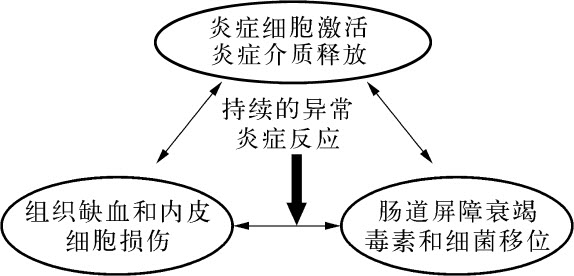
\includegraphics{./images/Image00002.jpg}
 \captionsetup{justification=centering}
 \caption{多器官功能障碍综合征的发病机制}
 \label{fig1-1}
  \end{figure} 

(1)炎症反应学说 炎症反应学说是MODS发病机制的基石。研究表明,感染或创伤引起的毒素释放和组织损伤并不是导致器官功能衰竭的直接原因,细菌和(或)毒素和组织损伤所诱发的全身炎症反应是导致器官功能衰竭的根本原因。

(2)缺血再灌注和自由基学说 缺血再灌注和自由基也是导致MODS的重要机制之一。MODS的自由基学说主要包括3方面:①氧输送不足导致组织细胞直接的缺血缺氧性损害;②缺血再灌注促发自由基大量释放;③白细胞与内皮细胞的互相作用,导致组织和器官损伤,最终发生MODS。从根本上来看,自由基学说也是炎症反应学说的重要组成部分。

(3)肠道动力学说 肠道动力学说的概念最早是由Meakins和Marshall提出的。肠道是机体最大的细菌和毒素库,肠道有可能是MODS患者菌血症的来源。另外,MODS患者菌血症的细菌往往与肠道菌群一致。因此,Meakins和Marshall提出肠道可能是MODS发生发展的动力器官(gut
motor)。在感染、创伤或休克时,即使没有细菌的移位,肠道内毒素的移位也将激活肠道及其相关的免疫炎症细胞,导致大量炎症介质的释放,参与MODS的发病。因此,肠道是炎症细胞激活、炎症介质释放的重要场地之一,也是炎症反应失控的策源地之一。从这一点来看,肠道动力学说实际上是炎症反应学说的一部分。

\subsubsection{全身炎症反应失衡怎样导致多器官功能障碍综合征的发生?}

基于全身炎症反应综合征是导致多器官功能障碍综合征(MODS)的根本原因这一认识,抑制全身炎症反应综合征有可能阻断炎症反应发展,最终可能降低MODS的病死率。20世纪90年代初期,大量的动物实验研究显示,抑制炎症介质能够明显降低感染或内毒素血症动物的病死率,这为临床MODS的救治带来希望。令人失望的是,内毒素单抗、肿瘤坏死因子α单抗等炎症介质拮抗剂在临床试验中相继失败,甚至个别研究报道增加病死率。由此迫使人们深入研究,并重新认识全身炎症反应综合征在MODS中的作用。

首先,引起注意的是机体受细菌毒素、损伤打击后,出现一过性细胞免疫功能降低,使机体对感染易感;其次,机体受细菌毒素、损伤刺激后,不仅释放炎症介质引起全身炎症反应综合征,同时大量释放内源性抗炎介质,后者可能是导致机体免疫功能损害的主要原因;第三,临床上盲目使用炎症介质拮抗剂,可能使免疫功能损伤加重,或许这就是炎症介质拮抗剂临床试验失败的主要原因。鉴于上述认识,1996年Bone针对感染或创伤时,导致机体免疫功能降低的内源性抗炎反应,提出了代偿性抗炎反应综合征(compensatory
anti-inflammatory response
syndrome,CARS)的概念。代偿性抗炎反应综合征作为全身炎症反应综合征的对立面,两者常常是不平衡的。如保持平衡,则内环境稳定得以维持,不会引起器官功能损伤。一旦全身炎症反应综合征和代偿性抗炎反应综合征失衡,将引起内环境失去稳定性,导致组织器官损伤,发生MODS
\protect\hyperlink{text00007.htmlux5cux23ch7-6}{\textsuperscript{{[}7{]}}}
\textsuperscript{,}
\protect\hyperlink{text00007.htmlux5cux23ch8-6}{\textsuperscript{{[}8{]}}}
。

如果把全身炎症反应综合征和代偿性抗炎反应综合征看作机体炎症反应天平的两端,则代偿性抗炎反应综合征作为天平的另一端,对全身炎症反应综合征发生、发展所起的关键性作用是不言而喻的。代偿性抗炎反应综合征的发生主要与抗炎性介质合成、抗炎性内分泌激素及炎症细胞凋亡等因素有关。

就其本质而言,MODS是全身炎症反应综合征和代偿性抗炎反应综合征免疫失衡的严重后果。全身炎症反应综合征和代偿性抗炎反应综合征失衡导致MODS的发展过程可分为3个阶段:①局限性炎症反应阶段,局部损伤或感染导致炎症介质在组织局部释放,诱导炎症细胞向局部聚集,促进病原微生物清除和组织修复,对机体发挥保护作用;②有限全身炎症反应阶段,少量炎症介质进入循环诱发全身炎症反应综合征,诱导巨噬细胞和血小板向局部聚集,同时,由于内源性抗炎介质释放增加导致代偿性抗炎反应综合征,使全身炎症反应综合征与代偿性抗炎反应综合征处于平衡状态,炎症反应仍属生理性,目的在于增强局部防御作用;③全身炎症反应综合征和代偿性抗炎反应综合征失衡阶段,表现为两个极端,一是大量炎症介质释放入循环,刺激炎症介质瀑布样释放,而内源性抗炎介质又不足以抵消其作用,导致全身炎症反应综合征;另一个极端是内源性抗炎介质释放过多而导致代偿性抗炎反应综合征。全身炎症反应综合征和代偿性抗炎反应综合征失衡的后果是炎症反应失控,使其由保护性作用转变为自身破坏性作用,不但损伤局部组织,同时打击远隔器官,导致MODS。

认识的进步,必然预示着在治疗上取得突破。恢复全身炎症反应综合征和代偿性抗炎反应综合征的动态平衡可能是MODS治疗的关键。

\subsubsection{多器官功能障碍综合征的二次打击学说有何临床意义?}

多器官功能障碍综合征(MODS)往往是多元性和序贯性损伤的结果,而不是单一打击的结果。1985年Dietch提出MODS的二次打击学说,将创伤、感染、烧伤、休克等早期直接损伤作为第一次打击,第一次打击所造成的组织器官损伤是轻微的,虽不足以引起明显的临床症状,但最为重要的是,早期损伤激活了机体免疫系统,尽管炎症反应的程度较轻,但炎症细胞已经被动员起来,处于预激活状态。此后,如病情稳定,则炎症反应逐渐缓解,损伤组织得以修复;如病情进展恶化或继发感染、休克等情况,则构成第二次或第三次打击。第二次打击使已处于预激活状态的机体免疫系统爆发性激活,大量炎症细胞活化、炎症介质释放,结果炎症反应失控,导致组织器官的致命性损害。第二次打击强度本身可能不如第一次打击,但导致炎症反应的爆发性激活,往往是致命性的(图\ref{fig1-2})。

\begin{figure}[!htbp]
 \centering
 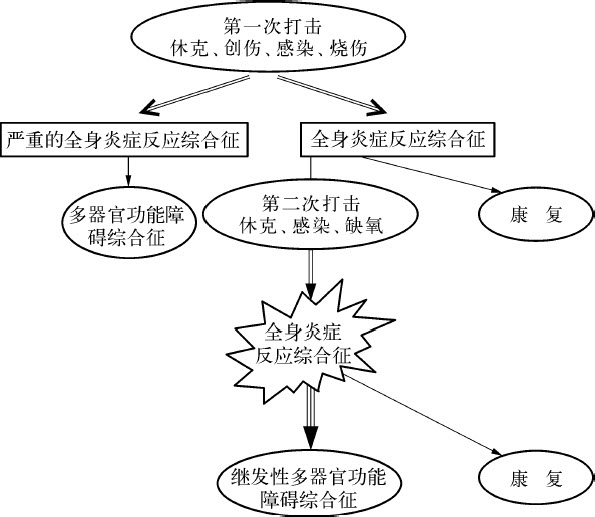
\includegraphics{./images/Image00003.jpg}
 \captionsetup{justification=centering}
 \caption{多器官功能障碍综合征的二次打击学说}
 \label{fig1-2}
  \end{figure} 

当第一打击强度足够大时,可直接强烈激活机体炎症反应,导致MODS,属于原发性MODS。但大多数患者MODS是多元性和序贯性损伤的结果,并不是单一打击的结果,这类MODS属于继发性MODS。常见的第二次打击包括继发性感染、休克、缺氧、缺血、创伤、手术等。对于多发性创伤的患者,如创伤严重,则直接可导致MODS,但多数患者经早期清创处理后基本稳定,而创伤早期发生的低血压导致各器官发生不同程度的缺血再灌注损伤及巨噬细胞、中性粒细胞激活,使患者出现发热、白细胞升高等炎症反应表现。创伤后3~7天,继发性感染或休克,使已处于预激活或激活状态的炎症细胞发生爆发性激活,结果使炎症反应失控,导致自身组织器官的损害,最终发展为MODS。

危重患者的病情往往是复杂的,机体遭受打击次数可能是两次,也可能是多次。多次反复打击将使机体炎症反应放大和失控更易发生,使患者更易发生MODS。另外,不仅机体免疫系统参与多次打击导致MODS的病理生理过程,凝血、纤溶、补体、激肽等多个系统均参与或累及。

MODS二次打击学说的提出,进一步强调了感染、创伤的后期处理。后期处理不当,其后果比早期损伤的结果更为严重,更具危害性。

\subsubsection{多器官功能障碍综合征有哪些临床特征?}

尽管多器官功能障碍综合征(MODS)的临床表现很复杂,但在很大程度上取决于器官受累的范围及损伤是由一次打击还是由多次打击所致。MODS临床表现的个体差异很大,一般情况下,MODS病程为14~21天,并经历4个阶段,包括休克、复苏、高分解代谢状态和器官衰竭阶段。每个阶段都有其典型的临床特征(表\ref{tab1-2}),且发展速度极快,患者可能死于MODS的任一阶段。

\begin{table}[htbp]
\centering
\caption{MODS的临床分期和特征}
\label{tab1-2}
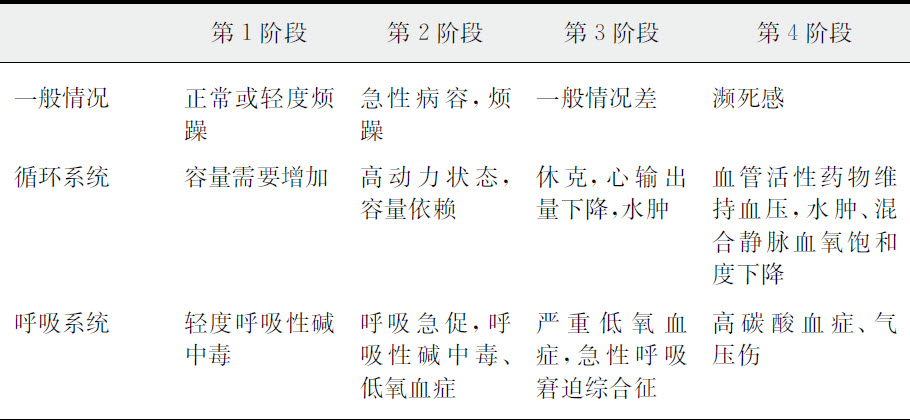
\includegraphics[width=\textwidth,height=\textheight,keepaspectratio]{./images/Image00004.jpg}
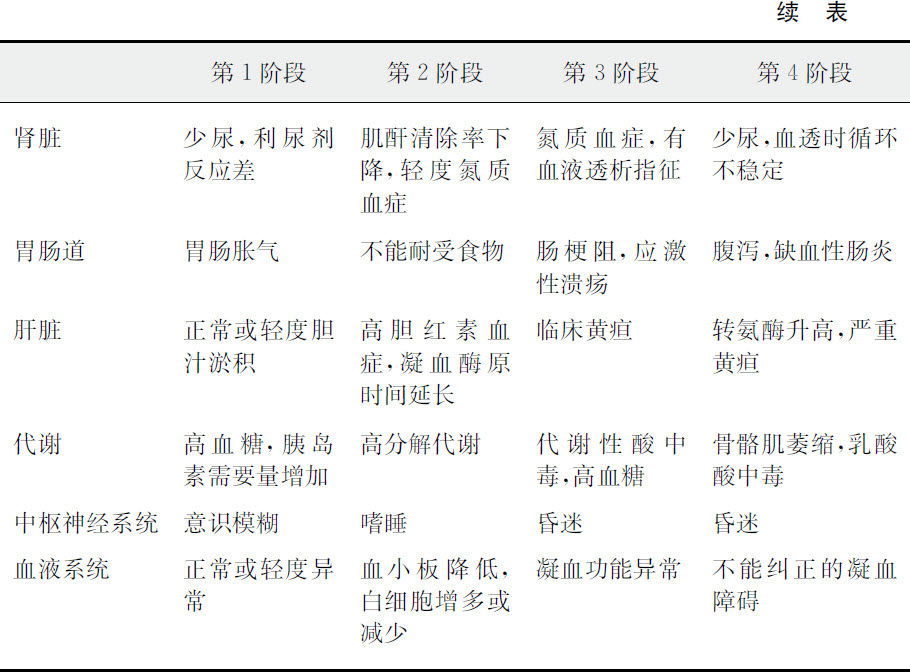
\includegraphics[width=\textwidth,height=\textheight,keepaspectratio]{./images/Image00005.jpg}
\end{table}



\subsubsection{不同多器官功能障碍综合征诊断标准有何差异?}

1980年Fry提出第一个多器官功能衰竭诊断标准。在此之前,循环、呼吸、肾脏和肝脏等器官已经具有单一器官衰竭的判断或诊断标准。应激性上消化道出血被认为是胃肠道功能衰竭。然而,血液、代谢和神经系统的衰竭或功能紊乱就缺乏明确的诊断方法。DIC显然是血液系统的功能紊乱,DIC诊断中除了出血等临床表现外,还需有血浆纤维蛋白降解产物水平升高。但血浆纤维蛋白降解产物浓度升高缺乏特异性,严重创伤或手术患者也可升高,使血液系统功能衰竭的诊断缺乏客观性。代谢紊乱是重症患者应激的结果,如果能够对代谢过程进行复杂的监测,则所有重症患者可能都存在所谓的“代谢障碍”,对代谢障碍的诊断缺乏可行性。神经系统功能障碍在重症患者中也很常见,但准确定量评价非常困难。另外,严重感染导致内脏器官严重损害时,往往血压和心输出量是正常或偏高的,直到出现休克或临终期,心血管系统才表现出功能衰竭。因此,Fry在提出多器官功能衰竭诊断标准时,仅包含了呼吸、肝脏、肾脏和胃肠道系统(表\ref{tab1-3})。

\begin{table}[htbp]
\centering
\caption{多器官功能衰竭诊断标准(Fry,1980年)}
\label{tab1-3}
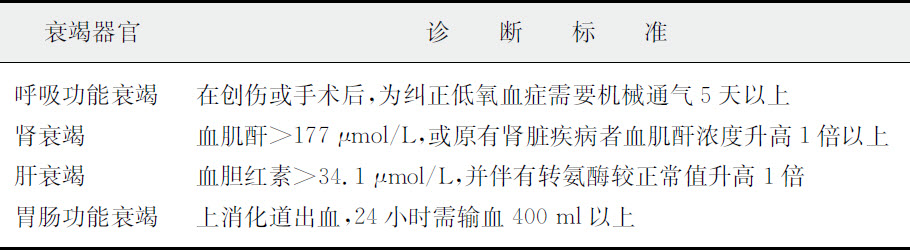
\includegraphics[width=\textwidth,height=\textheight,keepaspectratio]{./images/Image00006.jpg}
\end{table}

尽管Fry的多器官功能衰竭诊断标准是目前被公认的、应用最普遍的诊断标准,仍然存在很多问题:①该标准未包括神经系统、循环系统、血液系统等常见的器官功能衰竭;②以终末期的功能衰竭为诊断标准,不利于早期诊断和治疗;③难以反映多器官功能衰竭动态连续变化的病理生理过程;④呼吸功能衰竭的诊断过于严格,容易漏诊。

针对Fry诊断标准存在的问题,我们于1997年提出了修正的Fry-多器官功能障碍综合征(MODS)诊断标准(表\ref{tab1-4}),该标准结合国际常用的诊断标准,几乎包括了所有可能累及的器官或系统。当然,该标准未能包括MODS的整个病理生理过程,但避免了繁琐的程度评分,较为简捷,增加了临床实用性。

\begin{table}[htbp]
\centering
\caption{MODS诊断标准}
\label{tab1-4}
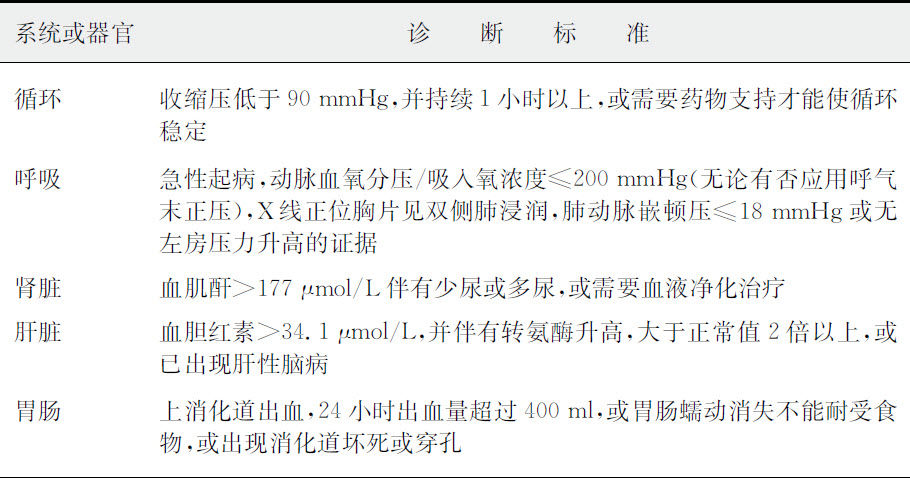
\includegraphics[width=\textwidth,height=\textheight,keepaspectratio]{./images/Image00007.jpg}
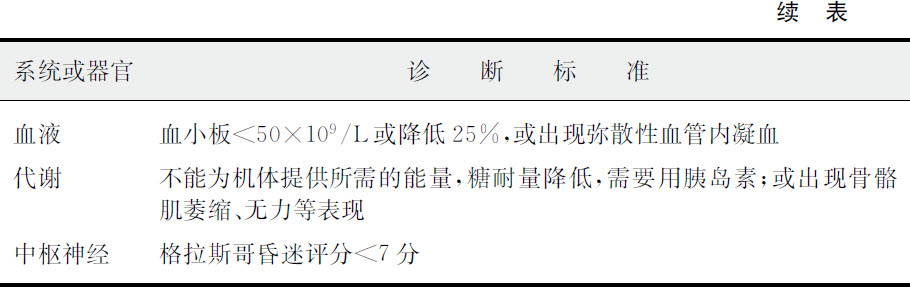
\includegraphics[width=\textwidth,height=\textheight,keepaspectratio]{./images/Image00008.jpg}
\end{table}

\subsubsection{哪些因素导致多器官功能障碍综合征的病死率增加?}

多器官功能障碍综合征(MODS)患者病死率高,认识病死危险因素,有助于早期确立MODS治疗对策。Knaus等学者对MODS的病死危险因素做了大规模的临床调查,概括了MODS病死的相关危险因素(表\ref{tab1-5})。\footnote{* APACHE:急性生理和慢性健康状况评分。}

\begin{table}[htbp]
\centering
\caption{MODS的病死危险因素}
\label{tab1-5}
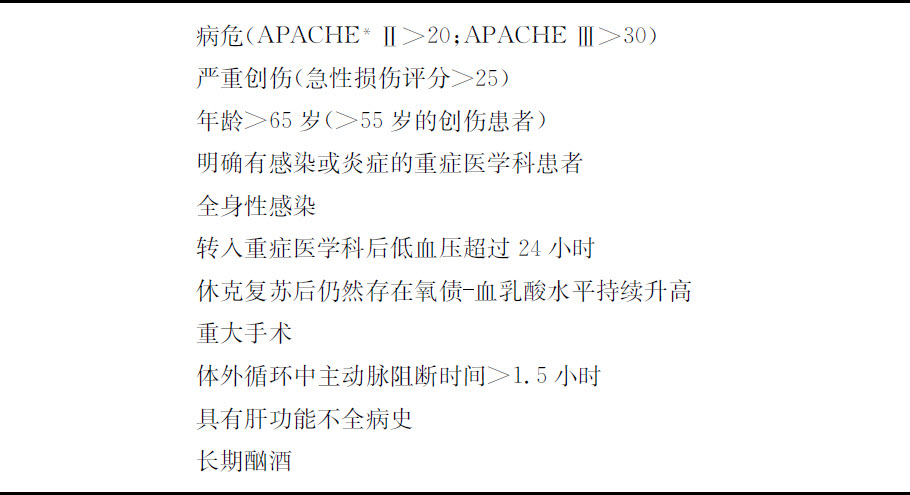
\includegraphics[width=\textwidth,height=\textheight,keepaspectratio]{./images/Image00009.jpg}
\end{table}

我国的研究也显示,免疫功能低下、转入ICU时的急性生理和既往健康评分(APACHE)Ⅱ评分、非手术、感染性休克及器官衰竭数目等因素与MODS患者死亡的关系显著。创伤、感染等MODS的病因、全身炎症反应综合征程度等因素与患者病死率无明显关系。

循环功能衰竭,即感染性休克为MODS最常见的直接病死原因;其次为中枢神经系统功能衰竭和心功能衰竭等,进一步提示在MODS治疗中,应特别注意纠正循环衰竭,并针对病因采取有效治疗措施,不应掉以轻心。

总之,MODS病死率依然很高,针对MODS病死危险因素进行积极处理和干预,可能是降低MODS病死率的关键。

\subsubsection{多器官功能障碍综合征时免疫功能障碍的基本概念是什么?}

免疫功能障碍不仅是多器官功能障碍综合征(MODS)的重要组成部分,同时在MODS发生发展中发挥关键的作用。MODS免疫功能障碍包括机体过度或失控炎症反应和免疫功能麻痹的动态过程。炎症反应本质上属于免疫反应的范畴,失控的炎症反应是MODS发生发展的根本机制,严重的炎症反应或细胞因子风暴可迅速引起微循环衰竭和感染性休克,继而发生DIC、呼吸衰竭和肝肾等器官功能障碍。免疫功能抑制可能与免疫效应细胞减少或功能抑制、机体呈调节T细胞或Th2极化和抗炎介质释放增多等因素有关。

临床免疫功能障碍可表现为多器官功能障碍,可于数小时、数天或数周发病,病程也长短不一。如爆发型流脑、中毒性休克综合征及严重猪链球菌Ⅱ型感染等严重炎症反应常在很短的时间内迅速发生休克、呼吸衰竭、肾衰竭和DIC等。免疫功能抑制患者常表现为原发感染难以痊愈,潜在感染的复发,或出现新的继发性感染。目前准确定量评价机体炎症反应水平和免疫功能紊乱性质、程度仍存在困难,还缺乏准确的临床判断指标和诊断方法。通过仔细的临床观察和密切的实验室检测,早期诊断器官功能损害或衰竭,并给予强化的器官功能支持治疗,能够避免部分患者死于继发性器官功能衰竭。

尽管MODS中免疫功能衰竭日益受到重视,然而由于其功能复杂性,免疫功能障碍缺乏明确的定义,亦无公认的临床判断指标。对免疫复杂而精细调节的反应和机制进行研究,从而充分发挥机体的防御作用,对减少损伤、促进机体康复是非常必要的。

\subsubsection{哪些是多器官功能障碍综合征时合并免疫功能障碍的主要病因?}

(1)感染 全身性感染(sepsis)是临床上引起免疫功能障碍常见的原因,如肺部感染、腹腔感染、血流感染、尿路感染及皮肤感染等。爆发型流脑、严重猪链球菌Ⅱ型感染及某些类型链球菌、葡萄球菌感染所致中毒性休克综合征等也是临床常见的免疫功能紊乱性疾病。

(2)创伤、烧伤、手术 许多非感染因素如严重创伤、大手术等也可以活化炎细胞,如变性坏死的组织细胞及其产物、缺氧、免疫复合物等。有研究证实,创伤程度越重,机体免疫抑制效应越强,表现为单核细胞功能降低、淋巴细胞增殖受到抑制、白介素-2合成减少等,继发感染并发症是导致伤员死亡的主要原因之一。

(3)急性胰腺炎 胰腺细胞受损首先导致局部炎症反应,细胞因子进入血液循环可致白细胞激活,引发全身炎症反应综合征和多器官功能障碍综合征(MODS)。重症急性胰腺炎可在数小时或数天病情迅速加重,甚至在早期发生MODS而危及生命。

(4)营养不良 临床研究表明,危重病人营养不良的发生迅速而普遍,且营养不良本身已成为预测危重症预后不良风险的重要因素。由于营养素摄入不足、消耗增加或代谢异常等导致机体营养不良,引起胸腺和淋巴组织早期就受到损害,致使免疫功能低下,容易并发各种感染。

(5)免疫性疾病 免疫组织、细胞或分子存在结构、数量或功能缺陷,导致免疫防御功能损害,表现为抗感染能力下降,易发生反复或持续感染,如白细胞减少症、粒细胞缺乏症。

(6)其他疾病 如慢性消耗性疾病、恶性肿瘤等。最近研究发现脑卒中诱导的免疫抑制(stroke-induced
immunosuppression)可导致卒中后感染并发症增加
\protect\hyperlink{text00007.htmlux5cux23ch9-6}{\textsuperscript{{[}9{]}}}
。

(7)医源性因素 某些药物如免疫抑制剂、化疗药物、放疗等可显著抑制机体免疫功能。

\subsubsection{多器官功能障碍综合征免疫功能障碍的发病机制是什么?}

免疫功能障碍发病机制复杂,多种因素交互促成,且有待深入研究。严重感染、创伤后机体免疫功能发生紊乱,既可能表现为亢进,也可能低下,且往往表现为早期炎症反应亢进,后期发生免疫功能抑制
\protect\hyperlink{text00007.htmlux5cux23ch10-6}{\textsuperscript{{[}10{]}}}
。

(1)早期炎症反应亢进 炎症反应与免疫反应关系密切。遇到损伤信号后,机体吞噬细胞、NK细胞等迅速动员,执行防卫功能,吞噬、杀伤或抑制细菌或其他小颗粒,如果被吞噬的颗粒较大,吞噬细胞无法将其包围,或细胞损伤崩解,则颗粒内容物将逸出而损伤邻近正常组织。

严重感染、创伤早期,各种免疫细胞和多种体液因子参与早期炎症反应,吞噬细胞如中性粒细胞、单核细胞和巨噬细胞等活化,补体系统激活。活化的炎细胞释放的炎症介质一般在局部发挥防御作用,血浆中一般测不出炎症介质。全身炎症反应综合征时,大量炎细胞活化,分泌的炎症介质溢出到血浆中。炎症时细胞因子往往呈序贯性表达和不同幅度的升高,大量释放的炎症因子、毒素、蛋白酶导致组织细胞损伤。随着病情好转,血浆中炎症介质减少。在爆发型流脑、中毒性休克综合征、严重猪链球菌Ⅱ型感染及急性爆发型胰腺炎等,引起严重的炎症反应或暴风式炎症反应(细胞因子风暴),很短的时间内剧烈的炎症反应迅速引起休克和多器官功能障碍综合征
\protect\hyperlink{text00007.htmlux5cux23ch11-6}{\textsuperscript{{[}11{]}}}
\textsuperscript{,}
\protect\hyperlink{text00007.htmlux5cux23ch12-6}{\textsuperscript{{[}12{]}}}
。

(2)免疫功能抑制 免疫功能抑制又称免疫麻痹(immunoparalysis),常引起机体继发感染,甚至因严重感染而死亡,其发病机制复杂,可能与以下因素有关。

吞噬细胞减少或功能抑制,重症患者往往因为高血糖、应用免疫抑制剂、放化疗等引起白细胞减少、粒细胞缺乏等。

树突状细胞减少或功能抑制,树突状细胞数量减少参与全身性感染免疫抑制发生。研究观察到,全身性感染小鼠3天发现脾脏树突状细胞数量明显减少。临床研究也观察到,严重感染和感染性休克的患者循环髓系树突状细胞和浆细胞样树突状细胞均明显减少
\protect\hyperlink{text00007.htmlux5cux23ch13-6}{\textsuperscript{{[}13{]}}}
\textsuperscript{,}
\protect\hyperlink{text00007.htmlux5cux23ch14-6}{\textsuperscript{{[}14{]}}}
。树突状细胞的抗原提呈能力降低与免疫抑制也有关。Poehlmann等观察到,存在免疫麻痹的严重感染和感染性休克患者,循环髓系树突状细胞和浆细胞样树突状细胞均明显减少,人类白细胞相关抗原-DR表达明显降低,且至28天仍低于正常。Kawasaki等也证实在创伤后小鼠脾脏树突状细胞的抗原提呈能力明显下降。

免疫效应细胞减少:严重感染和感染性休克患者免疫效应细胞减少参与免疫抑制。Hotchkiss等观察到,对严重感染及感染性休克死亡的患者行尸检发现脾脏CD4\textsuperscript{+}
T细胞和B细胞显著减少,且这些免疫效应细胞明显减少主要系细胞凋亡所致。在重症医学科中因严重感染死亡的患儿尸检结果同样证实脾脏CD4\textsuperscript{+}
T细胞和B细胞显著减少。上述研究提示免疫效应细胞大量丢失介导免疫抑制发生。

负性免疫调节细胞增多:机体内调节T细胞发挥负性免疫调控效应。研究发现,合并免疫麻痹的感染性休克患者病程第1~2天,外周血调节T细胞绝对数和相对比例均即明显升高,第3~6天进一步增加,与存活组相比,死亡组患者调节T细胞持续升高。提示调节T细胞可能与免疫抑制有关。

细胞因子表达谱改变:全身性感染病程中细胞因子分泌异常也与免疫抑制相关。Kawasaki等发现创伤后小鼠脾脏树突状细胞分泌白介素-12明显减少。Wen等研究显示,盲肠结扎穿孔小鼠脾脏白介素-12均明显降低,而抗炎细胞因子白介素-10则明显升高。说明细胞因子谱表达异常参与全身性感染的免疫抑制发生。

\subsubsection{多器官功能障碍综合征免疫功能障碍的病理改变有哪些表现?}

免疫功能障碍患者免疫器官可出现各种类型、程度不一的病理改变。

炎症反应主要是机体对损伤或感染的防御反应,以变质、渗出和增生为基本病理特征。脏器损害复杂多样,病变程度轻重不一,可出现某一个或多个脏器突出损害表现。组织可仅轻微的炎症反应,也可呈现明显的白细胞浸润。

免疫抑制患者的免疫器官可出现明显异常。有研究观察到,严重感染及感染性休克患者脾脏大量CD4\textsuperscript{+}
T细胞和B细胞凋亡,而CD8\textsuperscript{+}
T细胞、自然杀伤细胞和巨噬细胞无明显变化。另有研究发现,全身炎症反应综合征患者中性粒细胞往往表现为凋亡延迟,生存周期的延长,造成过度的炎症反应而损伤组织
\protect\hyperlink{text00007.htmlux5cux23ch15-6}{\textsuperscript{{[}15{]}}}
\textsuperscript{,}
\protect\hyperlink{text00007.htmlux5cux23ch16-6}{\textsuperscript{{[}16{]}}}
。

\subsubsection{多器官功能障碍综合征免疫功能障碍的病理生理改变特点是什么?}

多器官功能障碍综合征(MODS)免疫功能障碍包括机体过度或失控炎症反应和免疫功能麻痹的动态过程。由于众多细胞因子和体液介质的复杂作用,引起一系列复杂的病理生理改变,严重威胁患者生命。

炎症反应主要是机体对损伤或感染的防御反应。炎症细胞聚集和激活可释放各种蛋白酶,有利于溶菌、杀菌和水解清除已破坏或衰老的细胞组分,适当浓度的细胞因子有调节细胞识别、募集、迁移和组织修复的作用。但即使是有益的反应也难免有正常组织受损,如果炎症反应失衡或失控,细胞因子大量或全身释放则具有毒性,将造成过度或持续的组织损伤,尤其是对血管基膜、内皮细胞和基质成分,引起多器官损伤。

炎细胞活化分泌的炎症介质又导致炎细胞活化,二者互为因果,形成炎症瀑布。一般情况下,炎细胞活化只出现在损伤局部,而全身炎症反应综合征时可发生在远隔部位,如肝枯否细胞,或血循环带到远隔部位
\protect\hyperlink{text00007.htmlux5cux23ch17-6}{\textsuperscript{{[}17{]}}}
。众多细胞因子间可相互诱生,相互调节分泌,相互调控受体表达,其生物效应也互相影响,可协调、叠加,或起拮抗作用,因此形成了复杂的细胞因子网络。

细菌或毒素作用下,大量炎细胞浸润,并释放多种细胞因子(如白介素-1、白介素-6和肿瘤坏死因子-α等)和趋化因子等,内毒素作用下引起微循环衰竭和感染性休克,继而迅速发生DIC、MODS等则是其主要病理生理学基础。有的表现为全身感染中毒症状。有时由于极微量的毒素就可能非特异性激活大量的免疫细胞,引起过量的细胞因子释放,在数小时至数天造成暴风式炎症反应,导致广泛的组织细胞损伤和严重的毛细血管渗漏,结果在极短的时间内引起休克和MODS。如起病急骤、剧烈的炎症反应和迅速发生MODS是爆发型流脑、中毒性休克综合征、严重猪链球菌Ⅱ型感染及急性爆发型胰腺炎等重要的病理生理特征
\protect\hyperlink{text00007.htmlux5cux23ch18-6}{\textsuperscript{{[}18{]}}}
\textsuperscript{,}
\protect\hyperlink{text00007.htmlux5cux23ch19-6}{\textsuperscript{{[}19{]}}}
。细菌致病成分复杂,与细菌的免疫生物学特征密切相关,主要包括细菌外毒素、内毒素、胞外酶等致病因子,活化免疫细胞,促进释放大量TNF-α等炎症性细胞因子,导致机体免疫功能紊乱。

\subsubsection{多器官功能障碍综合征免疫功能障碍的临床表现是哪些?}

免疫功能障碍可表现为全身炎症反应或免疫功能低下。

(1)全身炎症反应 全身炎症反应可呈急骤起病,表现为全身感染中毒症状如畏寒、寒战、高热,可出现皮疹。爆发型流脑、中毒性休克综合征及严重猪链球菌Ⅱ型感染等在数小时至数天发病,潜伏期很短。

(2)器官功能障碍 爆发型流脑、中毒性休克综合征及严重猪链球菌Ⅱ型感染后等常在很短的时间内迅速发生休克和多器官功能障碍综合征,早期常合并呼吸衰竭、肾衰竭和DIC等器官功能衰竭。通过仔细的临床观察和密切的实验室检测,早期诊断器官功能损害或衰竭,并给予积极的治疗,明显能够预防患者死于继发性的器官功能衰竭。对病死患者的死亡原因做归因分析,也证实强化的器官功能支持治疗,能够避免患者死于继发性器官功能衰竭。

(3)感染 免疫功能抑制患者临床表现为原发感染难以痊愈、潜在感染的复发,或出现新的继发性感染。感染的性质和严重程度主要取决于免疫功能缺陷的成分及其程度。Otto等回顾性调查16041例重症患者,观察到严重感染或感染性休克后期免疫抑制的患者机会性细菌和真菌感染显著增加。由于免疫功能低下发生的感染,一般多发生在病程1周以后。需要注意的是,免疫抑制患者由于全身反应差,临床上可无明显发热、白细胞升高等表现。另外,免疫功能抑制者尤其是细胞免疫抑制者,恶性肿瘤的发病率也可能升高。

\subsubsection{多器官功能障碍综合征免疫功能障碍的诊断包括哪些内容?}

目前准确定量评价机体免疫功能紊乱性质和程度仍存在困难,还缺乏准确的临床判断指标和诊断方法。血浆或组织中的某些炎症介质和(或)免疫细胞的某些变化有可能成为免疫功能障碍的较为特异的诊断指标,但目前尚不完全成熟,仍有待临床资料的积累。

临床上全身炎症反应与全身炎症反应综合征诊断标准一致,但全身炎症反应综合征标准不能评估炎症反应水平。C反应蛋白和一些细胞因子如肿瘤坏死因子-α、白介素-6、白介素-8及高迁移率族蛋白B-1等可用于评估全身炎症反应,但C反应蛋白存在升高、降低较慢,与炎症反应程度关系不确切,在判断炎症反应水平的价值方面并非不存在问题。细胞因子作为生化标记物具有广阔的前景,但因其往往存在半衰期短及检测方法标准化问题而有待完善。

循环中单核细胞和粒细胞数量和功能作为常用的判断免疫功能检测指标之一。

动态定量评估单核细胞表面人类白细胞相关抗原-DR表达是临床常用的衡量细胞免疫功能指标。表达率<30%或<5000分子/细胞提示免疫功能低下。需要注意检测抗体、流式细胞仪及检测方案标准化,以保证实验结果可比较,同时血标本应用乙二胺四乙酸抗凝是必要的。

单核细胞分泌促炎细胞因子如肿瘤坏死因子-α的能力也是评估免疫反应功能指标。脂多糖刺激全血后产生肿瘤坏死因子-α<300pg/ml是判断免疫麻痹标准。仍然需要注意细胞因子检测的标准化问题。

T淋巴细胞极性分化如Th1/Th2/调节T细胞检测在动物和临床研究中取得了一定价值,但仍待完善。

\subsubsection{多器官功能障碍综合征免疫功能障碍的治疗原则是哪些?}

(1)控制原发病 原发病处理是多器官功能障碍综合征(MODS)和免疫功能障碍治疗的基础和关键。治疗中应早期去除或控制诱发免疫功能障碍的病因,避免机体再次打击。若为创伤患者,则应积极清创,并预防感染发生。对于存在严重感染的患者,必须注意感染灶的寻找和处理,积极引流感染灶,应用有效抗生素进行治疗。

(2)免疫调理治疗 目前已明确无论是过度免疫激活还是免疫抑制都对机体不利,针对此改变实施的免疫调理策略,恢复免疫功能稳态,是有效解决免疫功能障碍的重要措施。对于免疫抑制患者,免疫刺激治疗有望改善预后
\protect\hyperlink{text00007.htmlux5cux23ch20-6}{\textsuperscript{{[}20{]}}}
。对于炎症反应亢进患者,通过调节早期免疫过度激化,有助重建机体免疫内稳状态,可能有助于减轻组织炎症反应,改善生存率。值得注意的是,免疫调节治疗的前提是准确判断机体免疫状态,缺乏免疫监测的情况下不恰当的免疫干预可能适得其反。

(3)器官功能支持治疗 爆发型炎症反应患者起病急骤,迅速发生多器官功能衰竭。因此,一旦出现器官功能衰竭的早期征兆,应积极给予强有力的器官功能支持措施,避免器官功能损害进一步发展。如对于休克患者,液体复苏的时机和速度至关重要,以迅速纠正有效循环血量不足、快速逆转休克。对于DIC,一旦发生血小板、纤维蛋白原明显降低或D-二聚体明显升高,立即补充新鲜冰冻血浆、冷沉淀、血小板,并积极给予小剂量低分子肝素治疗。一旦出现呼吸衰竭、肾衰竭的早期征兆,立即给予积极的机械通气和肾脏替代治疗。

(4)激素治疗 炎症反应强烈或休克不能逆转或多器官功能迅速发生衰竭时,可积极给予糖皮质激素,但对免疫的抑制作用又不利于感染的控制。小剂量氢化考的松(每日200mg分次静脉滴注)、长疗程(7天)补充糖皮质激素可以降低严重感染和感染性休克肾上腺皮质功能不全患者的28天病死率和对血管活性药物的依赖性。“短程”(<24~48小时)、“大剂量”(甲基泼尼松龙30mg/kg,每4~6小时一次)应用糖皮质激素治疗对严重感染和感染性休克患者的预后没有改善,但在细胞因子风暴如爆发型流脑、中毒性休克综合征、严重猪链球菌Ⅱ型感染及急性爆发型胰腺炎等应用指征、方法及对预后的确切影响并不清楚,尚待进一步研究阐明。

(5)连续性肾脏替代治疗 早期连续性肾脏替代治疗和血浆交换可通过滤过和吸附等清除血浆中的炎症介质和毒素,调节内环境紊乱,达到控制全身炎症反应的目的,且有助于防止器官损害。现认为应采用高流量血滤。

(6)控制血糖 严重应激状态下,机体常出现代谢性高血糖反应及外周胰岛素抵抗。高血糖可抑制吞噬细胞功能。血糖升高已成为一独立因素直接影响重症患者的预后。多项临床研究表明,严格血糖控制可改善各类重症患者的预后,特别是外科重症患者。因此,正确处理各类危重患者的应激性高血糖,同时避免低血糖的发生,对于提高综合治疗效果,改善生存率具有重要的意义。

(7)营养支持 由于免疫功能障碍的复杂性和病因存在显著差异,其营养支持的很多重要问题仍然没有取得共识。一般认为早期肠内营养支持促进胃肠蠕动,减轻肠黏膜萎缩,保护胃肠道屏障功能。谷氨酰胺是免疫细胞的营养底物,可适量补充。精氨酸作为一氧化氮合成的底物,在上调机体免疫功能与炎症反应方面具有“双刃剑”的作用。严重感染病人应避免应用富含精氨酸的免疫营养制剂。

\subsubsection{多器官功能障碍综合征免疫功能抑制的预后如何?}

爆发型流脑、休克型猪链球菌Ⅱ型感染、中毒性休克综合征等爆发型炎症反应患者,病程凶险,预后差。国内研究观察到休克型猪链球菌Ⅱ型感染多器官功能衰竭发生率高达86.7%,这也是休克型猪链球菌患者高病死率的重要原因。急性爆发型胰腺炎表现为发病后数日内迅速发展为多器官功能衰竭,病死率也极高。

免疫抑制患者往往因为原发感染难以治愈或继发新的感染,或发生多器官功能障碍综合征而预后明显变差。有研究观察到,单核细胞表面HLA-DR作为免疫功能衰竭标志,持续低表达院内感染发生率显著升高,且可预测感染性休克患者病死率
\protect\hyperlink{text00007.htmlux5cux23ch21-6}{\textsuperscript{{[}21{]}}}
。

总之,危重患者合并免疫功能障碍是困惑临床医生的难题,也是医学的热点问题,因此,必须高度重视免疫功能障碍的严峻形势,探索规范的诊断手段和有效的治疗手段,最终改善免疫功能障碍患者预后。

\subsubsection{多器官功能障碍综合征的治疗应注意哪些原则?}

多器官功能障碍综合征(MODS)患者应入住重症医学科,但MODS患者的监测和治疗应由专科医师和重症医学科专职医师共同完成。尽管MODS的病因复杂、涉及的器官和系统多、治疗中往往面临很多矛盾,但MODS的治疗应遵循以下原则。

(1)积极控制原发病 控制原发疾病是MODS治疗的关键,应重视原发疾病的处理。对于存在严重感染的患者,必须积极引流感染灶和应用有效抗生素。若为创伤患者,则应积极清创,并预防感染的发生。当重症患者出现腹胀、不能进食或无石性胆囊炎时,应采用积极的措施,如导泻、灌肠等,以保持肠道通畅,恢复肠道屏障功能,避免肠源性感染。而对于休克患者,则应争分夺秒地进行休克复苏,尽可能地缩短休克时间,避免引起进一步的器官功能损害。

(2)改善氧代谢和纠正组织缺氧 氧代谢障碍是MODS的特征之一,纠正组织缺氧是MODS重要的治疗目标。改善氧代谢障碍、纠正组织缺氧的主要手段包括增加全身氧输送、降低全身氧需、改善组织细胞利用氧的能力等。提高氧输送是目前改善组织缺氧最可行的手段。氧输送是单位时间内心脏泵出的血液所携带的氧量,由心脏泵功能、动脉氧分压/血氧饱和度和血红蛋白浓度决定,因此,提高氧输送也就通过心脏、血液和肺交换功能3个方面来实现。降低氧需在MODS治疗中常常被忽视。镇静、降低体温、机械通气等均是降低氧需的重要手段。由于组织缺氧是氧供和氧需失衡的结果,氧需增加也是导致组织缺氧和MODS的原因之一,降低氧需对MODS的防治具有重要意义。MODS和休克可导致全身血流分布异常,肠道和肾脏等内脏器官常常处于缺血状态,持续的缺血缺氧,将导致急性肾衰竭和肠道功能衰竭,加重MODS。因此,改善内脏灌注是MODS治疗的重要方向。

(3)代谢支持与调理 MODS使患者处于高度应激状态,导致机体出现以高分解代谢为特征的代谢紊乱。机体分解代谢明显高于合成代谢,蛋白质分解、脂肪分解和糖异生明显增加,但糖的利用能力明显降低,有学者将之称为自噬现象(autocannibalism)。严重情况下,机体蛋白质分解代谢较正常增加40%~50%,而骨骼肌的分解可增加70%~110%,分解产生的氨基酸部分经糖异生作用后供能,部分供肝脏合成急性反应蛋白。器官及组织细胞的功能维护和组织修复有赖于细胞得到适当的营养底物,机体高分解代谢和外源性营养利用障碍,可导致或进一步加重器官功能障碍。因此,在MODS早期,代谢支持和调理的目标应当是试图减轻营养底物不足,防止细胞代谢紊乱,支持器官、组织的结构功能,参与调控免疫功能,减少器官功能障碍的产生;而在MODS的后期,代谢支持和调理的目标是进一步加速组织修复,促进患者康复。

(4)免疫调节治疗 基于炎症反应失控是导致MODS的根本原因这一认识,抑制全身炎症反应综合征有可能阻断炎症反应发展,最终可能降低MODS病死率。免疫调控治疗实际上就是MODS病因治疗的重要方面。当前,对机体炎症反应认识的深入,取得了阶段性的成果,但要对MODS治疗发挥指导性作用,尚有待时日。

总之,全面深刻地认识和研究MODS的发病机制,采用积极合理的干预手段,必将提高MODS的治疗成功率。

\begin{center}\rule{0.5\linewidth}{\linethickness}\end{center}

参考文献

\protect\hyperlink{text00007.htmlux5cux23ch1-6-back}{{[}1{]}}
.邱海波,周韶霞.多器官功能障碍综合征现代治疗.人民军医出版社.

\protect\hyperlink{text00007.htmlux5cux23ch2-6-back}{{[}2{]}} .Johnson
D,Mayers I.Multiple organ dysfunction syndrome:a narrative
review.Can J Anesth,2001,48:502-509.

\protect\hyperlink{text00007.htmlux5cux23ch3-6-back}{{[}3{]}} .Marshall
JC.SIRS and MODS:what is their relevance to the science and practice
of intensive care?Shock,2000,14:586-589.

\protect\hyperlink{text00007.htmlux5cux23ch4-6-back}{{[}4{]}} .Bhatia
M,Neoptolemos JP,Slavin J.Inflammatory mediators as therapeutic
targets in acute pancreatitis.Curr Opin Investig
Drugs,2001,2:496-501.

\protect\hyperlink{text00007.htmlux5cux23ch5-6-back}{{[}5{]}} .Deitch
EA,Xu D,Kaise VL.Role of the gut in the development of injury - and
shock induced SIRS and MODS:the gut-lymph hypothesis,a review.Front
Biosci,2006,11:520-528.

\protect\hyperlink{text00007.htmlux5cux23ch6-6-back}{{[}6{]}} .Aird
WC.The role of the endothelium in severe sepsis and multiple organ
dysfunction syndrome.Blood,2003,101:3765-3777.

\protect\hyperlink{text00007.htmlux5cux23ch7-6-back}{{[}7{]}} .Knotzer
H,Pajk W,Dünser MW,etal.Regional microvascular function and vascular
reactivity in patients with different degrees of multiple organ
dysfunction syndrome.Anesth Analg,2006,102:1187-1193.

\protect\hyperlink{text00007.htmlux5cux23ch8-6-back}{{[}8{]}} .Baue
AE.MOF,MODS,and SIRS:what is in a name or an
acronym?Shock,2006,26:438-449.

\protect\hyperlink{text00007.htmlux5cux23ch9-6-back}{{[}9{]}} .Marshall
JC.Modeling MODS:what can be learned from animal models of the
multiple-organ dysfunction syndrome?Intensive Care
Med,2005,31:605-608.

\protect\hyperlink{text00007.htmlux5cux23ch10-6-back}{{[}10{]}} .Fink
MP,Delude RL.Epithelial barrier dysfunction:a unifying theme to
explain the pathogenesis of multiple organ dysfunction at the cellular
level.Crit Care Clin,2005,21:177-196.

\protect\hyperlink{text00007.htmlux5cux23ch11-6-back}{{[}11{]}}
.Olanders K,Sun Z,Borjesson A,et al.The effect of intestinal
ischemia and reperfusion injury on ICAM - 1 expression,endothelial
barrier function,neutrophil tissue influx,and protease inhibitor
levels in rats.Shock,2002,18:86-92.

\protect\hyperlink{text00007.htmlux5cux23ch12-6-back}{{[}12{]}}
.Schroder O,Laun RA,Held B,et al.Association of interleuk in - 10
promoter polymorphism with the incidence of multiple organ dysfunction
following major trauma:results of a prospective pilot
study.Shock,2004,21:306-310.

\protect\hyperlink{text00007.htmlux5cux23ch13-6-back}{{[}13{]}}
.Mueller KL.Innate immunity.Recognizing the first
responders.Introduction.Science(80-).2010.327:283.

\protect\hyperlink{text00007.htmlux5cux23ch14-6-back}{{[}14{]}} .Akira
S,Uematsu S,Takeuchi O.Pathogen recognition and innate
immunity.Cell.2006.124:783-801.

\protect\hyperlink{text00007.htmlux5cux23ch15-6-back}{{[}15{]}} .Zhu
J,Yamane H,Paul WE.Differentiation of effector CD\textsubscript{4} T
cell populations(*).Annu Rev Immunol.2010.28:445-489.

\protect\hyperlink{text00007.htmlux5cux23ch16-6-back}{{[}16{]}} .Meisel
C,Meisel A.Suppressing immunosuppression after stroke.N Engl J
Med.2011.365:2134-2136.

\protect\hyperlink{text00007.htmlux5cux23ch17-6-back}{{[}17{]}}
.Hotchkiss RS,Coopersmith cm,McDunn JE,Ferguson TA.The sepsis
seesaw:tilting toward immunosuppression.Nat Med.2009.15:496-497.

\protect\hyperlink{text00007.htmlux5cux23ch18-6-back}{{[}18{]}}
.Hotchkiss RS,Nicholson DW.Apoptosis and caspases regulate death and
inflammation in sepsis.Nat Rev Immunol.2006.6:813-822.

\protect\hyperlink{text00007.htmlux5cux23ch19-6-back}{{[}19{]}}
.Hotchkiss RS,Opal S.Immunotherapy for sepsis - a new approach
against an ancient foe.N Engl J Med.2010.363:87-89.

\protect\hyperlink{text00007.htmlux5cux23ch20-6-back}{{[}20{]}} .Meisel
C,Schefold JC,Pschowski R,et al.Granulocyte-macrophage
colony-stimulating factor to reverse sepsis-associated
immunosuppression:a double-blind,randomized,placebo-controlled
multicenter trial.Am J Respir Crit Care Med.2009.180:640-648.

\protect\hyperlink{text00007.htmlux5cux23ch21-6-back}{{[}21{]}}
.Landelle C,Lepape A,Voirin N,et al.Low monocyte human leukocyte
antigen -- DR is independently associated with nosocomial infections
after septic shock.Intensive Care Med.2010.36:1859-1866.

\protect\hypertarget{text00008.html}{}{}


\chapter{发 热}

\section{【发热的定义与病因】}

正常人的体温在体温调节中枢的调节下,产热与散热处于动态平衡之中,维持人体的体温在相对恒定的范围之内。口腔温度(舌下测温)范围约为36.3~37.2℃,直肠内温度一般比口腔约高0.3~0.5℃,腋窝温度比口腔约低0.2~0.4℃。

在生理状态下,不同的个体,同一个体不同的时间和不同的环境,其体温会有所不同:①不同个体:儿童由于代谢率高,体温可比成年人高;老年人代谢率低,体温比成年人低;个别人的基础体温可比正常范围略高或略低0.5℃左右。②同一个体不同时间:正常情况下,人体体温在早晨较低,下午较高,但一般波动范围不超过1℃;妇女在排卵期和妊娠期体温较高,月经期较低。③不同环境:运动、进餐、情绪激动和高温环境下工作时体温较高,低温环境下体温较低。

在病理状态下,由于各种不同原因致人体产热增多或(及)散热减少,使体温升高超过正常范围时,就称为发热。一般来说,口腔温度在37.3℃以上,或直肠温度在37.6℃以上,可认为有发热。临床上按热度高低将发热分为低热(37.3~38℃)、中等度热(38.1~39℃)、高热(39.1~41℃)及超高热(41℃以上)。

引起发热的病因很多,按有无病原体侵入人体分为感染性发热和非感染性发热两大类。

\subsection{(一)感染性发热}

引起感染性发热的病原体有细菌、病毒、支原体、立克次体、螺旋体、真菌及寄生虫等。各种病原体侵入人体后可引起相应的疾病,不论急性还是慢性、局灶性还是全身性均可引起发热。病原体及其代谢产物或炎性渗出物等外源性致热原,在体内作用于致热原细胞如中性粒细胞、单核细胞-巨噬细胞等,使其产生并释放白细胞介素-1、干扰素、肿瘤坏死因子及炎症蛋白-1等而引起发热。感染性疾病占发热病因的50\%~60\%。

\subsection{(二)非感染性发热}

由病原体以外的其他病因引起的发热称为非感染性发热。常见于以下原因:

\subsubsection{1.吸收热}

由于组织坏死、组织蛋白分解和坏死组织吸收引起的发热称为吸收热。

\paragraph{(1)物理和机械性损伤:}

大面积烧伤、创伤、大手术后、骨折、内脏出血和热射病等。

\paragraph{(2)血液系统疾病:}

白血病、恶性淋巴瘤、恶性组织细胞病、骨髓增生异常综合征、多发性骨髓瘤、急性溶血、血型不合输血等。

\paragraph{(3)肿瘤性疾病:}

血液恶性肿瘤之外的各种恶性肿瘤。

\paragraph{(4)血栓栓塞性疾病:}

①静脉血栓形成:如股静脉血栓形成。②动脉血栓形成:如心肌梗死、肺动脉栓塞。③微循环血栓形成:如血栓性血小板减少性紫癜、弥散性血管内凝血等。

\subsubsection{2.变态反应性发热}

变态反应产生的抗原抗体复合物成为外源性致热原,激活了致热原细胞,使其产生并释放白细胞介素-1、干扰素、肿瘤坏死因子及炎症蛋白-1等引起的发热。如风湿热、药物热、血清病以及各种结缔组织病(如系统性红斑狼疮、多发性肌炎与皮肌炎、结节性多动脉炎等)。

\subsubsection{3.中枢性发热}

有些致热因素不通过内源性致热原而直接损害体温调节中枢,使体温调定点上移后发出调节冲动,造成产热大于散热,体温升高,称为中枢性发热。这类发热的特点是高热无汗。如:

(1)物理因素:如中暑等。

(2)化学因素:如重度安眠药中毒等。

(3)机械因素:如颅内出血或颅内肿瘤细胞浸润等。

(4)功能性因素:如自主神经功能紊乱和感染后低热等。

\subsubsection{4.其他}

如甲状腺功能亢进、痛风、严重脱水、因致热原引起的输液或输血反应等。

\section{【发热疾病的检查】}

\subsection{(一)问诊}

发热的病因复杂,常造成诊断上的困难。认真细致的问诊常能为进一步检查提供重要提示。问诊的要点包括:①起病时间、季节、起病情况(缓急)、病程、程度(热度高低)、频度(间歇性或持续性)、诱因。②有无畏寒、寒战、大汗或盗汗。③多系统症状询问,如是否伴有皮疹、出血、黄疸、咳嗽、咳痰、咯血、胸痛、腹痛、呕吐、腹泻、尿频、尿急、尿痛、头痛、肌肉关节痛等。④患病以来一般情况,如精神状态、食欲、体重改变及睡眠。⑤诊治经过(拟诊、药物、剂量、疗效)。⑥传染病接触史、疫水接触史等流行病学资料;手术史、流产或分娩史、用药史、职业特点等。兹就其中一些重要问题再强调如下:

\subsubsection{1.病史}

详细询问病史往往为发热的诊断与鉴别诊断提供重要线索。例如传染病的流行病学资料十分重要,如蚊虫叮咬可引起乙型脑炎、疟疾、登革热等;有牧区逗留与牲畜接触史者可患布鲁菌病;1个月内有血吸虫病疫水接触史者可引起急性血吸虫病。发热前2~3周内有无皮肤外伤及疖肿史,如有是诊断葡萄球菌败血症的重要线索。在用药过程中出现原因未明发热要注意药物热的可能。大量使用广谱抗生素、糖皮质激素、免疫抑制剂等引起二重感染(机会感染)而致发热不退,或热退后又再发热者亦时有见之。

\subsubsection{2.发热的特点}

\paragraph{(1)发热的临床过程和特点:}

1)体温上升期:体温上升有两种方式:①骤升型:体温在几小时内达39℃以上,常伴有寒战。见于疟疾、大叶性肺炎、败血症、流行性感冒、急性肾盂肾炎、输液或输血反应等。②缓升型:体温逐渐上升在数日内达高峰,多不伴寒战。如伤寒、结核病、布鲁菌病等所致的发热。

2)高热期:是指体温上升达高峰之后保持一定时间。不同疾病持续时间长短不等。如疟疾可持续数小时,大叶性肺炎、流行性感冒可持续数天,伤寒则可长达数周。

3)体温下降期:①骤降型:指体温于数小时内迅速下降至正常,有时可略低于正常,常伴有大汗淋漓。常见于疟疾、急性肾盂肾炎、大叶性肺炎和输液反应等。②渐降型:指体温在数天内逐渐降至正常,如伤寒、风湿热等。

\paragraph{(2)热型:}

不同病因所致发热的热型也常不同:

1)稽留热:体温恒定地维持在39~40℃以上的高水平,达数天或数周。24小时内体温波动范围不超过1℃。常见于大叶性肺炎、恙虫病、流行性脑脊髓膜炎、斑疹伤寒及伤寒的高热期。

2)弛张热:又称败血症热型。体温常在39℃以上,24小时内体温波动范围超过2℃,但都在正常水平以上。常见于败血症、风湿热、重型肺结核及化脓性炎症等。

3)间歇热:体温骤升达高峰后持续数小时,然后迅速降至正常水平,无热期(间歇期)可持续1至数天。如此高热期与无热期反复交替出现。可见于疟疾、急性肾盂肾炎、淋巴瘤、败血症等。

4)波状热:体温逐渐上升达39℃或以上,数天后又逐渐下降至正常水平,持续数天后又逐渐升高,如此反复多次。常见于布鲁菌病、登革热等。

5)回归热:体温急骤上升至39℃或以上,持续数天后又骤然回复到正常水平,高热期与无热期各持续若干天后规律性交替1次。可见于回归热、霍奇金淋巴瘤、周期热等。

6)不规则热:发热的体温曲线无一定规律,可见于结核病、风湿热、支气管肺炎、渗出性胸膜炎、流行性感冒、败血症等。

一般说来,热程短、高热、寒战等中毒症状者,有利于感染性疾病的诊断;如热程中等,但呈渐进性消耗、衰竭者,以结核和恶性肿瘤多见;热程长,无毒血症状,发作与缓解交替出现,则有利于结缔组织病的诊断。

\subsubsection{3.发热的伴随症状}

\paragraph{(1)寒战:}

常见于大叶性肺炎、败血症、急性肝胆道感染、急性肾盂肾炎、流行性脑脊髓膜炎、疟疾、钩端螺旋体病、药物热、急性溶血、输血或输液反应等。

\paragraph{(2)全身状况:}

渐进性消瘦衰竭见于结核、恶性肿瘤等;不少结缔组织病早期精神、食欲及体重可无明显变化。

\paragraph{(3)各系统症状:}

可提示疾病的部位。皮疹与多种急性发热性疾病(参见第2节)和慢性发热性疾病相关。

\subsection{(二)体格检查}

全面而细致的体格检查非常重要,兹重点讨论如下:

\subsubsection{1.一般状况及全身皮肤黏膜检查}

注意全身营养状况。恶病质提示重症结核、恶性肿瘤。注意有无皮疹及皮疹类型:斑疹见于斑疹伤寒、丹毒;面部蝶形红斑、指端及甲周红斑提示为系统性红斑狼疮;环形红斑见于风湿热;丘疹和斑丘疹见于猩红热、药物热;玫瑰疹见于伤寒和副伤寒。睑结膜及皮肤少许瘀点,指端、足趾、大小鱼际肌有压痛的Osler小结节见于亚急性感染性心内膜炎;软腭、腋下条索状或抓痕样出血点见于流行性出血热;耳廓、跖趾、掌指关节等处结节为痛风石,见于痛风患者;皮肤散在瘀点、瘀斑、紫癜见于再生障碍性贫血、急性白血病及恶性组织细胞瘤;大片瘀斑提示弥散性血管内凝血。皮肤和软组织的化脓性病灶,常为发热病因,或败血症的来源。皮肤巩膜出现黄疸提示肝、胆道疾病、溶血性疾病和中毒性肝损害。

\subsubsection{2.淋巴结检查}

注意全身浅表淋巴结有无肿大。局部淋巴结肿大、质软、有压痛者,要注意相应引流区有无炎症。局部淋巴结肿大、质硬、无压痛,可能为癌肿转移;局部或全身淋巴结肿大、质地韧实有弹性、无压痛者可能为淋巴瘤;全身淋巴结肿大尚可见于急慢性白血病、传染性单核细胞增多症、系统性红斑狼疮等。

\subsubsection{3.头颈部检查}

结膜充血多见于流行性出血热、斑疹伤寒、麻疹;扁桃体肿大,其上有黄白色渗出物可以拭去,为化脓性扁桃体炎;外耳道流出脓性分泌物为化脓性中耳炎;乳突红肿伴压痛为乳突炎、鼻窦压痛点有压痛提示鼻窦炎。检查颈部时注意有无阻力,阻力增加或颈项强直提示为脑膜刺激,见于脑膜炎或脑膜脑炎。甲状腺弥漫性肿大、质软(血管杂音)提示为甲状腺功能亢进。

\subsubsection{4.心脏检查}

胸廓隆起常提示心脏肥大;胸骨下段压痛提示白血病、恶性组织细胞病;心脏扩大和新出现的收缩期杂音提示为风湿热;原有心瓣膜病,病程中杂音性质改变,需考虑感染性心内膜炎,应予查超声心动图、血培养。

\subsubsection{5.肺部检查}

一侧肺局限性叩浊、语颤增强,有湿啰音,提示为大叶性肺炎;下胸部或背部固定或反复出现湿啰音,见于支气管扩张伴继发感染;一侧肺下部叩浊、呼吸音及语颤减低,提示胸腔积液;大量积液时患侧胸廓饱满,气管移向健侧,在年轻患者中以结核性胸膜炎多见,也可见于恶性肿瘤侵犯胸膜或结缔组织病。

\subsubsection{6.腹部检查}

右上腹压痛、Murphy征阳性伴皮肤巩膜黄染,提示为胆囊炎、胆石症发热;中上腹明显压痛、胁腹部皮肤见灰紫斑(Grey-Turner征)或脐周皮肤青紫(Cullen征),甚至上腹部可触及肿块,见于坏死性胰腺炎;转移性腹痛伴麦氏点压痛,多为阑尾炎;右下腹或全腹疼痛伴明显压痛,有时在右下腹或脐周扪及腹块,腹壁或会阴部有瘘管并有粪便与气体排出,全身营养较差,可能为克罗恩病;全腹压痛、反跳痛见于腹膜炎;肝大、质硬、表面有结节或巨块,提示为肝癌;肝脾同时肿大,可见于白血病、淋巴瘤、恶性组织细胞病、系统性红斑狼疮、败血症等。季肋点压痛、肾区叩击痛、提示上尿路感染。

\subsubsection{7.四肢检查}

杵状指(趾)伴发热,可见于肺癌、肺脓肿、支气管扩张、感染性心内膜炎等。多关节红肿、压痛见于风湿热、系统性红斑狼疮、类风湿关节炎。化脓性关节炎、结核性关节炎、痛风的早期常侵犯单个关节。发热伴有肌肉疼痛见于许多急性传染病,一般无特征性诊断意义。如腓肠肌剧烈疼痛,甚至不能站立与行走,常提示钩端螺旋体病。多发性肌肉显著疼痛可见于多发性肌炎或皮肌炎。

\subsubsection{8.神经系统检查}

发热伴意识障碍或(及)脑膜刺激征见于中枢神经系统感染、中枢神经系统白血病或其他肿瘤。应注意发热兼有中枢神经系统症状、体征者,不少起源于急性全身感染、内分泌代谢障碍、结缔组织病、中毒等全身性疾病,但这些疾病多有相应病史和临床表现,应注意与中枢神经系统疾病鉴别。

\subsection{(三)实验室及辅助检查}

实验室检查及器械检查可补充病史与体检的不足,尤其对一些仅以发热为主要症状而缺乏明确反映脏器损害的症状和体征的患者,往往有重要的诊断与鉴别诊断意义。血、尿、大便常规与X线胸片属发热的常规检查。血培养应列为未明原因发热的常规检查。其他检查根据临床提示,有针对性地选择应用。

\subsubsection{1.血常规检查}

白细胞计数及分类对发热的鉴别诊断有重要初筛价值。白细胞总数及中性粒细胞升高,提示为细菌性感染,尤其是化脓性感染;也见于某些病毒感染如流行性出血热;成人Still病、风湿热亦有白细胞增多。极度白细胞增多见于白血病及类白血病反应。大多数病毒感染无白细胞增多,甚至减少;这一现象亦可见于某些细菌感染(如伤寒或副伤寒、结核病的某些类型)和某些原虫感染(如疟疾、黑热病)。嗜酸性粒细胞增多见于寄生虫病、变态反应性疾病等;在伤寒时,嗜酸性粒细胞消失是一个有力的诊断支持点,有助于与其他急性传染病鉴别。绝对性淋巴细胞增多,见于传染性单核细胞增多症、传染性淋巴细胞增多症、百日咳、淋巴细胞性白血病等;淋巴细胞减少,见于大多数病毒性感染,如严重急性呼吸综合征(SARS)和高致病性禽流感肺炎等。全血细胞减少伴发热,见于恶性组织细胞病、重型再生障碍性贫血、白细胞减少的急性白血病、全身血行播散性结核病、癌肿骨髓转移、黑热病、艾滋病等。

\subsubsection{2.尿常规检查}

尿中白细胞增多,尤其是出现白细胞管型,提示急性肾盂肾炎;尿中出现红细胞,可见于尿道感染、败血症等。蛋白尿伴或不伴管型尿见于钩端螺旋体病、流行性出血热、系统性红斑狼疮等;蛋白尿也见于轻链型多发性骨髓瘤。

\subsubsection{3.大便常规检查}

隐血试验阳性、大便红、白细胞均提示有胃肠道病变。

\subsubsection{4.X线胸片}

伴有肺部病征的发热是发热的常见病因(参见第3节),且肺结核目前在我国仍然常见,因此X线胸片应列为发热的常规检查。

\subsubsection{5.血培养和骨髓培养}

血培养应列为未明原因发热(尤其具感染性血象者)的常规检查,该检查对败血症、伤寒或副伤寒、布鲁菌病、感染性心内膜炎等疾病的病因学诊断具有决定性意义。骨髓培养可提高诊断的敏感性。对长期使用广谱抗生素、糖皮质激素、免疫抑制剂及化疗药物者,或严重疾病状态全身衰竭患者,要注意真菌或厌氧菌感染的可能,应加做血真菌和厌氧菌培养。

\subsubsection{6.各种传染病的病原学及血清学检查}

目前我国仍有多种传染病流行,这类疾病构成国人急性发热的常见病因。再者,由于早期干预治疗,临床表现常不典型,因此病原学及血清学检查对这类疾病的及早确诊至关重要。可根据流行病学资料及临床表现的提示选择有关检查。

\subsubsection{7.骨髓涂片检查}

原因未明的长期发热(尤其伴进行性贫血者)是骨髓涂片检查的指征。该检查对各种血液病具有确诊的价值。

\subsubsection{8.结缔组织病相关检查}

原因未明的长期发热,疑有结缔组织病者可进行相关检查,包括血沉、C反应蛋白、蛋白电泳、免疫球蛋白、补体等常规项目,以及选择检查各种自身抗体如抗核抗体(ANA)谱、类风湿因子(RF)、抗中性粒细胞胞浆抗体(ANCA)、抗磷脂抗体等。

\subsubsection{9.影像学检查}

除了上述X线胸片作为常规检查外,根据临床提示可选择B超、CT、PET/CT、MRI用于胸、腹及颅内病灶的诊断;X线小肠钡剂造影用于消化道病变诊断;逆行胰胆管造影(ERCP)或磁共振胰胆管成像(MRCP)用于胆道病变诊断。

\subsubsection{10.内镜检查}

包括呼吸内镜(支气管镜、胸腔镜和纵隔镜),消化内镜(胃镜、结肠镜、小肠镜、胶囊内镜等),泌尿内镜(如膀胱镜),耳、鼻、咽喉镜等对诊断均有帮助。

\subsubsection{11.活体组织检查}

淋巴结活检对原因未明长期发热而兼有淋巴结肿大者往往能为诊断提供重要依据,阳性发现对淋巴结结核、淋巴瘤及癌的淋巴结转移有确诊价值。对某些诊断有困难的血液病如淋巴瘤、白血病、恶性组织细胞病、多发性骨髓瘤等骨髓活检可提高检出率。对诊断确有困难而有肝、脾大或腹膜后淋巴结或纵隔淋巴结肿大者,可考虑在B超或CT引导下行肝、脾、淋巴结穿刺或腹腔镜下取活检。支气管镜下病变组织活检对支气管癌及支气管内膜结核有确诊意义。

\subsubsection{12.其他}

疑感染性心内膜炎或心肌病者行超声心动图检查。疑中枢神经系统感染者行脑脊液检查。疑甲亢者行甲状腺功能检查。PPD皮试作为结核病的辅助检查。某些血清肿瘤标志物如AFP、CA19-9、CEA、CA125对消化系恶性肿瘤、PSA对前列腺癌具有辅助诊断价值。炎症标志物对发热的鉴别也有参考价值,如降钙素原、C-反应蛋白等。生化、肝功能、血清酶学检查对内分泌疾病、肝炎、心肌炎或心肌梗死、肌炎的诊断有帮助。

\section{【原因未明发热疾病的诊断性治疗】}

当病因经过各种检查尚难以查明时,在不影响进一步检查的情况下,可按可能性较大的病因进行诊断性治疗,观察治疗的效果,以助诊断。

\subsection{(一)诊断性治疗的原则和意义}

1.诊断性治疗仅适用于那些对拟诊疾病特异性强、疗效确切且安全性高的治疗药物的患者。

2.诊断性治疗一般否定的意义较肯定的意义大。例如患者经予氯喹的正规抗疟疗程仍不能退热,则疟疾的可能性很少,但反之并不尽然。因此,对诊断性治疗的效应要结合多方面作出恰当评价。

3.诊断性治疗剂量应充足,疗程要足,否则无助于判断。

用于诊断性治疗的药物有抗菌药物、抗原虫药物、抗风湿药物、抗肿瘤药物。例如拟诊疟疾用氯喹,拟诊结核予抗结核药物。

\subsection{(二)诊断性治疗注意事项}

应特别指出,诊断性治疗要慎用,使用不当,不但不起作用,反而会给诊断增加困难,甚至加重病情。兹就一些药物的应用强调如下:

\subsubsection{1.糖皮质激素的应用}

不要滥用糖皮质激素,以免改变原来热型和临床表现,给诊断带来困难;长期应用还会加重原有的感染或诱发新的感染,加重病情。因此,只在少数情况下,如高度怀疑为药物热、成人Still病且病情危急时,方可在有经验的医师指导下谨慎使用此类药物。

\subsubsection{2.抗菌药物的应用}

几乎所有的发热常因患者入院前均已接受了时间不等的抗生素治疗,抗生素诊断性治疗因此针对性不强,不仅干扰及时正确诊断治疗,而且容易导致耐药、二重感染或药物热。因此,应严格加以控制。仅对疑为感染性发热且病情危重的高热患者,在必要的实验室检查和各种培养标本采取后,根据初步临床诊断给予经验性抗菌治疗。

\subsubsection{3.退热药的应用}

确诊前使用退热药会改变热型、影响诊断。但对高热中暑、手术后高热、高热谵妄等应采取紧急降温措施。有条件时,可将室温调在27℃左右,采用物理或(及)药物降温,同时注意防止体温骤降伴大量出汗时可能导致的虚脱或休克。

\section{【发热疾病的分组】}

为便于进行鉴别诊断,从发热的缓急、程度、病程、特殊热型以及伴发的主要症状与体征等出发,将发热划分为急性发热、急性发疹性发热、伴有肺部病征的急性发热、周期性发热、长期发热以及慢性微热等6类,将在本章分别讨论,而伴有其他特别体征的发热,请参考各有关章节。

\protect\hypertarget{text00012.html}{}{}

\section{1 急性发热}

临床上一般将热程在2周以内的发热称为急性发热。急性发热临床常见,且不少为高热,其中以急性感染占首位,包括各种病原体引起的传染病,全身或局灶性感染。而各种病原体中又以细菌最为常见,其次为病毒。非感染的急性发热包括变态反应性疾病、风湿性疾病、组织坏死与血液分解产物的吸收、物理与化学因素、血液病与恶性肿瘤等。内科临床常见的急性发热疾病如表\ref{tab2-1}所示。

\begin{table}[htbp]
\centering
\caption{常见急性发热疾病的分类}
\label{tab2-1}
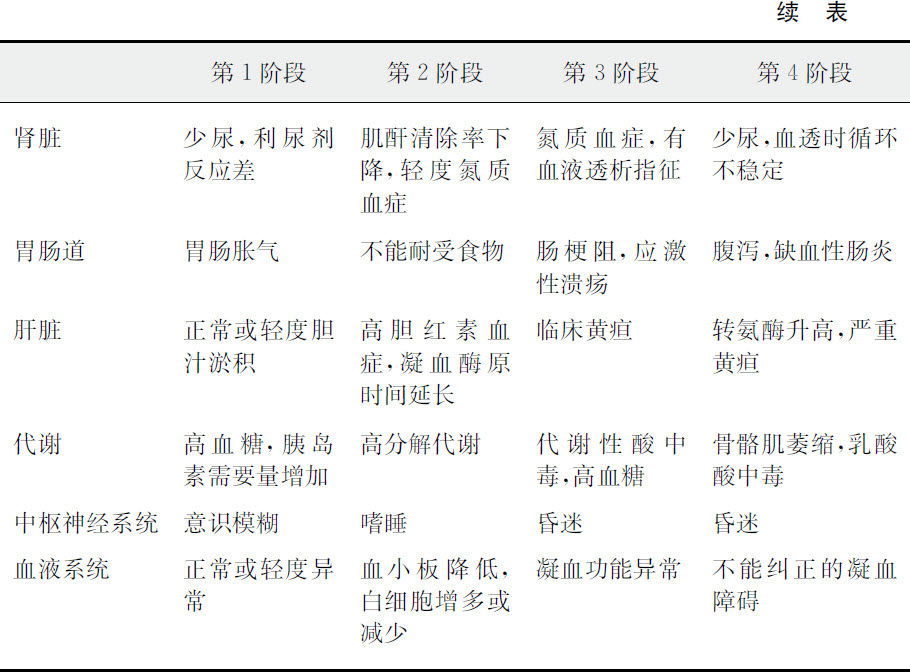
\includegraphics[width=5.92708in,height=6.28125in]{./images/Image00005.jpg}
\end{table}

急性发热性疾病病因很多,病史及临床表现典型者诊断较易,临床表现不典型的病例或较少见的疾病则会造成诊断的困难。因此,对于一时诊断未明的病例,鉴别诊断的思路要广,不但要熟悉常见病,也要了解少见病;不但要知道各种疾病的典型临床表现及实验室和辅助检查的诊断价值,也要不断积累在某特殊情况下临床表现不典型的疾病的诊断经验。本节主要讨论表\ref{tab2-1}中排黑体字的疾病,是在急性发热的鉴别诊断中较常遇到的疾病;以同时伴有皮疹为特征的急性发热性疾病放在“2.急性发疹性发热”一节中讨论;对伴有肺部病征的发热性疾病则只概要提及,详细讨论见“3.伴有肺部病征的急性发热”一节。

\protect\hypertarget{text00013.html}{}{}

\subsection{1.1 急性感染性发热}

急性感染性发热起病急,热度一般较高,多伴寒战或畏寒、全身肌肉和关节酸痛、头痛等毒血症状。一般可分为急性传染病和局限于某一脏器或组织的急性感染性疾病或(及)来源于局灶感染的败血症。前者往往有传染病的流行病学资料,后者多伴有局部症状和体征。细菌性感染多有周围血白细胞总数和中性粒细胞数升高。此外,血降钙素原(PCT)浓度>0.5ng/ml提示细菌感染,有助于与病毒感染、结核感染鉴别,且降钙素原水平与细菌感染的严重程度呈正相关。但也要注意降钙素原正常或轻度增高不能排除细菌感染的可能。而血清C反应蛋白在细菌感染时可呈中等度至明显升高。

\subsubsection{1.1.1 病毒性感染}

\paragraph{一、流行性感冒(流感)}

流行性感冒病毒可分为甲、乙、丙三型,其中甲型病毒易引起世界性流感大流行;乙型病毒则引起局部暴发和小流行;丙型病毒仅以散在形式出现。近几年新的病毒亚型如H5N1、H1N1和H7N9等出现流行或感染,需引起临床注意。

本病的潜伏期一般为1~7日,多数为2~4天。通常以突然畏寒、寒战、高热急骤起病,伴有全身酸痛、头痛、面潮红、结膜充血、虚弱无力等全身中毒表现,而呼吸道症状并不严重。血象白细胞总数减少,淋巴细胞相对增加。热程约3~5日。全身症状逐渐好转,但鼻塞、流涕、咽痛、干咳等上呼吸道症状逐渐显著。在流感多见的冬春季节,门诊上述症状的患者连续3日持续增加,并有直线上升趋势,或发热感冒患者2例以上的家庭连续增多,就应高度警惕本病的可能。对于非典型与散发病例,则易误诊为急性上呼吸道感染。但后者通常为非暴发流行、起病缓慢、症状较轻,上呼吸道症状较明显而无明显全身中毒症状。此外,流感亦易与多种早期的急性传染病如流行性脑脊髓膜炎、伤寒、副伤寒、支原体肺炎、军团菌病等相混淆,因此,须注意动态观察,以免造成误诊。

在流感流行时,根据接触史和典型临床表现诊断不难。特殊实验室检查可为确诊提供直接证据:①免疫荧光或免疫酶联染法检测抗原,取患者鼻洗液中黏膜上皮细胞涂片,用荧光或酶标记的流感病毒免疫血清染色检出抗原,快速且灵敏度高,有助于早期诊断。②用PCR测定流感病毒RNA,为直接、快速敏感的方法。③采样取患者起病3日内的含漱液或咽拭子做鸡胚接种或组织细胞接种培养分离病毒。④血清学检查:应用血凝抑制试验或补体结合试验检测急性期和恢复期(相隔2~4周)双份血清抗体效价,若升高4倍以上有诊断价值。

\paragraph{二、急性病毒性肝炎}

可有畏寒、发热,多呈中等度热,有些病例有明显的上呼吸道症状,类似感冒,少数患者出现关节痛,类似风湿热,应注意鉴别。但大多数患者有乏力、厌油、纳差、腹部不适或肝区、上腹部胀痛等症状。本期体征不显著或有肝大。故详细询问有无明显的消化道症状对诊断极有帮助。肝功能谷丙转氨酶升高,病毒性肝炎病毒检测或系列标志物的检测,有助于确诊。

\paragraph{三、流行性乙型脑炎(乙脑)}

初期典型表现为急性起病,早期发热,多为39℃以上高热,伴有头痛、恶心和呕吐,多有嗜睡和精神疲倦,可有抽搐,颈项强直。此后高热持续,出现意识障碍,如嗜睡、谵妄、昏迷、定向力障碍等,并出现惊厥或抽搐。有神经系统的体征如浅反射改变或脑膜刺激征,病理性锥体束征阳性等。轻型或普通型乙脑,可仅表现为头痛、发热、精神萎靡及嗜睡,此时常无神经系统体征,易致误诊。此时应仔细询问流行病学史[包括明显的季节性(7~9月份)、疫区、蚊虫叮咬史],脑脊液检查,血清补体结合试验、中和试验、血凝抑制试验和特异性IgM抗体测定有重要诊断价值。

\paragraph{四、脊髓灰质炎}

脊髓灰质炎发病的前驱期大多有发热,乏力不适,常伴有咽痛、咳嗽等上呼吸道症状。部分患者有恶心呕吐,腹痛腹泻等消化道症状。此期白细胞多数正常,而早期或合并感染时可增高,以中性粒细胞为主。上述表现无特异性,易误诊为上呼吸道感染或急性胃肠炎。但当发生在流行季节(夏秋季)如有易感者接触患者后出现上述症状应警惕本病。若发热不退,或热退后间歇1~6日,体温再次上升(称双峰热,为其典型的临床特征,见于10\%~30\%患者,小儿多见),并出现神经系统症状如头痛、肢体疼痛,感觉过敏,烦躁或嗜睡,体检出现颈背肌强直和阳性克氏征、布氏征,肌腱反射及浅反射减弱,则本病的可能性很大。此时脑脊液大多已有改变,呈无菌性炎症改变。与化脓性脑膜炎、结核性脑膜炎鉴别不难。但应注意与各种病毒性脑炎、流行性乙型脑炎鉴别。若出现弛缓性瘫痪则有利于本病的诊断。进入瘫痪期的本病患者,应与感染性多发性神经根炎鉴别。后者散发起病,不发热或仅有低热,逐渐出现弛缓性瘫痪,呈上行性、对称性,常伴感染障碍,脑脊液具有蛋白质增高而细胞少的分离现象为其特点。瘫痪恢复较快而完全,很少有后遗症。本病与引起轻瘫的其他病毒感染如柯萨奇、埃可病毒感染等区别,单从临床表现难以鉴别。确诊有赖于病毒分离及血清学检查。

确诊脊髓灰质炎需特殊的实验室检查:①病毒分离,起病1周内、从患者鼻咽部及粪便中分离出病毒,阳性率可达90\%,粪便可持续阳性2~3周。早期从血液和脑脊液中分离出病毒则更为可靠。②抗原检测:近年采用RT-PCR检测肠道病毒RNA,较组织培养快速敏感。③血清学检查:近年采用免疫荧光技术检测抗原及特异性IgM单克隆抗体酶标法检查,有助于早期诊断。

\paragraph{五、流行性出血热}

是一组以发热、出血、肾脏损害为主要临床表现的急性传染病。其病原体为汉坦病毒,鼠类为主要传染源。本病在我国全国各地均有报道,有明显季节性,有些地区该病流行高峰在5~6月份和10~12月份。

本病起病急骤,以畏寒、寒战、高热开始。体温可高达39~40℃,热型以弛张型为多。全身症状较重,表现为头痛、腰痛、眼眶痛(“三痛”)、畏光、视力模糊,颜面、上胸部及眼眶区明显充血(“三红”),似酒醉貌。

出血为常见症状,通常于发病第3~5日出现,皮肤黏膜、结膜、软腭、腋下可见散在针头大小的出血点或出血斑,有时密集的小点状出血排列成链条状,颇具诊断参考价值。出血点多见于上半身,尤其腋部与上胸部,这与一般紫癜不同。血小板大多减少,束臂试验每呈阳性。发热持续数天(一般3~7天),热退后症状反而加重并呈现低血压,有的甚至休克,为此病的重要特征之一。

患者有不同程度的肾脏损害表现。早期即可有蛋白尿及镜下血尿。有的病例在病程第5~7日可发生尿少甚至无尿,呈现急性肾小管坏死的病象,继而转入多尿期,以后逐渐康复。

本病典型的临床表现可达分为发热期、低血压期、少尿期、多尿期及恢复期五期。轻型病例病程较短,病情较轻。

本病早期应与上呼吸道感染、流行性感冒、伤寒、钩端螺旋体病等急性传染病及败血症相鉴别。有皮肤出血点应与血小板减少性紫癜相区别。当出现急性肾衰竭时,应与各种病因所致的急性肾衰竭相鉴别。本病有典型的临床表现和独特的临床经过,抗原检查和特异性抗体检查有助于早期诊断。近年采用多聚酶联反应(PCR)直接检测病毒抗原,有助于病原学诊断。

\paragraph{六、传染性单核细胞增多症}

本病是由EB病毒引起的一种急性或亚急性淋巴细胞良性增生的传染病。本病分布广泛,多呈散发性,以15~30岁的年龄组为多,流行性病例多见于儿童。发病多较急,多为中至高热,可呈弛张、不规则热或稽留热,热程自数日至数周。患者每有咽痛,咽峡炎相当常见,表现为咽、悬雍垂、扁桃体充血、肿大,其后可迅速出现斑状或膜状黄灰色苔膜,少数有溃疡和假膜形成。浅表淋巴结肿大亦相当常见,全身淋巴结均可累及,而以颈淋巴结肿大最为常见,通常无明显压痛。绝大多数病例有脾大,一般为轻中度肿大,约10\%患者有肝大并有肝功能异常,少数可出现黄疸。有时可出现斑疹或疱疹。病初起时白细胞计数正常,病后第10日左右白细胞总数有升高,分类中淋巴细胞增多;并出现异形淋巴细胞(10\%~30\%或更多)。本病病程多为1~3周,预后良好。

本病临床表现多种多样,常被误诊为急性咽炎、急性扁桃体炎、流感、病毒性肝炎、伤寒、血小板减少性紫癜、急性白血病或恶性淋巴瘤,少数神经系统受累者可误诊为乙型脑炎。周围血出现异形淋巴细胞(>10\%以上),是提示本病的重要线索。但异形淋巴细胞亦可见于某些其他病毒性感染如病毒性肝炎,流行性出血热等,但其数量一般<10\%。结合血清学检查可辅助诊断,嗜异凝集试验效价在1∶80以上具有诊断价值,若数周测定其效价上升4倍以上更有意义。但须注意,正常人、少数网状细胞瘤、单核细胞白血病、结核病亦可阳性,此时需吸附试验证实。

国外学者提出本病的诊断标准:①临床三联症:发热、咽峡炎、淋巴结病;②外周血淋巴细胞比例≥0.5和异形淋巴细胞比例≥0.1;③血清嗜异凝集抗体阳性。

\paragraph{七、巨细胞病毒感染}

正常成人巨细胞病毒(CMV)感染多表现为隐性感染,或单核细胞增多症表现,有发热、肝脾大,淋巴细胞相对或绝对增多,并出现异形淋巴细胞,与EB病毒所致的传染性单核细胞增多症相似,但巨细胞病毒感染咽痛和淋巴结肿大较少见,血清中无嗜异性凝集素及EB病毒抗体。免疫缺陷者的CMV感染,多发生在接受器官移植患者中,术后2~4个月多见,其首发临床表现为发热、乏力,可出现关节和肌肉疼痛以及全血细胞减少和异形淋巴细胞增多。病情进展快,肺部受累常见,可出现干咳、呼吸困难和进行性低氧血症,胸片两肺呈间质性、网状和结节状浸润,预后较差。检测特异性CMV-IgM抗体、CMV-DNA、CMV-PP65抗原阳性有助于急性和近期感染的诊断。血液或体液(主要为尿液)中分离出CMV病毒可确诊。

\paragraph{八、严重急性呼吸综合征}

严重急性呼吸综合征是2002年出现的由SARS冠状病毒(SARS-COV)引起的一种具有明显传染性、可累及多个脏器系统的特殊性肺炎,世界卫生组织(WHO)将其命名为严重急性呼吸综合征(SARS)。疫情暴发于温热带冬春之际,症状重,死亡率高。由于该病起病初期以发热为首发症状,呼吸道症状未出现或缺乏特异性,极易误诊为一般上呼吸道感染,如一旦延误诊断则会造成本病在与患者密切人群中的迅速播散。因此,在流行地区和流行季节要对本病保持高度警惕,有关本病的诊断与鉴别诊断参见第3.1节。

\protect\hypertarget{text00014.html}{}{}

\subsubsection{1.1.2 细菌性感染}

\paragraph{一、细菌性肺炎}

社区获得性肺炎常见细菌为肺炎链球菌、流感嗜血杆菌和卡他莫拉菌。患者常有受凉、劳累等诱因,通常急骤起病,以高热、寒战、咳嗽、血痰及胸痛为特征。本病早期或经抗生素治疗后上述症状和肺实变体征可不典型,易误导为未明原因的发热。因此,对心率和呼吸加速、血象白细胞总数增多者,应详细做胸部的体检。下叶肺炎刺激膈胸膜,胸痛可向腹部放射,易误诊为急腹症。胸部X线正侧位摄片,有助于早期做出诊断。

肺炎的临床诊断依据是:①新近出现的咳嗽、咳痰或原有呼吸道疾病症状加重,并出现脓性痰,伴或不伴胸痛。②发热。③肺实变体征和(或)闻及湿性啰音。④WBC>10×10\textsuperscript{9}
/L或<4×10\textsuperscript{9}
/L,伴或不伴细胞核左移。⑤胸部X线检查显示片状、斑片状浸润性阴影或间质性改变,伴或不伴胸腔积液。以上①~④项中任何1项加第⑤项,除外非感染性疾病可做出诊断。其他细菌或病原体引起的肺炎参见第3节。

\paragraph{二、感染性心内膜炎}

感染性心内膜炎指因细菌、真菌及其他微生物(如立克次体、衣原体等)直接感染心脏内膜表面,伴有赘生物形成。随着风湿性心脏病发病率的下降,风湿性心瓣膜病的感染性心内膜炎的发生率亦随之下降,而非风湿性瓣膜病的感染性心内膜炎发生率有所上升。加之,近年来日益增多的心血管疾病的创伤性检查、介入性治疗和人工心脏瓣膜的广泛应用,医源性感染性心内膜炎明显增加。静脉毒品滥用也增加了感染性心内膜炎的发病率。因此,对本病应保持警惕。

\subparagraph{(一)急性感染性心内膜炎}

本病常发生于原来无心脏病的患者。病原菌多为高毒力细菌和真菌,其中金黄色葡萄球菌约占50\%以上。本病往往起病突然,高热、寒战等全身毒血症状明显,病程常急骤凶险,易掩盖心内膜炎的局部临床表现。因心瓣膜和腱索的急剧损害,心脏可在短期内出现高调的杂音或原有杂音性质迅速改变,并可迅速发展为急性心力衰竭。故对败血症的患者,应注意心脏体征的改变,考虑本病的可能。如有多发性栓塞及多个器官、组织的转移性感染和脓肿出现,对诊断有重要提示。

累及右侧心脏的急性感染性心内膜炎,多见于安装心脏起搏器的老年患者,近年来由于静脉注射毒品成瘾者增多,右侧心脏心内膜炎的发病率亦明显增加。临床上除败血症表现外,常伴有咳嗽、胸痛、咳血痰和气急。累及三尖瓣者可闻及三尖瓣尖关闭不全的杂音,累及肺动脉瓣时可听到肺动脉瓣反流所致的舒张中期杂音。胸部X线可见多发性结节或片状炎症浸润,为三尖瓣或肺动脉瓣赘生物脱落所致的脓毒性肺梗塞。

急性感染性心内膜炎早期易漏诊,而后期病情危重,故诊断的关键是提高警惕,注意发现心脏及其他有关表现并密切观察病情变化。血培养和超声心动图对确诊有重要价值,详见下述。

\subparagraph{(二)亚急性感染性心内膜炎}

本病大多数发生在原有器质性心脏病的基础上,仅少数发生于正常的心脏。由于近年来普遍使用广谱抗生素,致病菌已发生明显改变,几乎所有的微生物都可引起本病,但草绿色链球菌仍是较常见的致病菌,肠球菌、表皮葡萄球菌、革兰氏阴性菌和真菌的比例则有增加。亚急性患者起病较缓慢。发热为最常见症状,以不规则热为多,也可为间歇热或弛张热,亦可仅有低热者。因此,原有器质性心脏病的患者发热一周以上,应考虑本病的可能。少数患者以贫血、顽固性心力衰竭、卒中、瘫痪、周围动脉栓塞等并发症的形式开始,因此,对原有心脏病患者,出现上述情况,亦应注意有否本病的存在。发热伴随的常见临床表现有皮肤黏膜瘀点、中等度贫血、蛋白尿和镜下血尿、脾大、心脏杂音等。白细胞数多数呈中度或轻度增高,少数可正常或减少,但分类中性粒细胞常增高。

由于近年来感染性心内膜炎的“经典”临床表现已不十分常见,尤其是皮肤和黏膜的瘀点、甲床下线状出血、Roth斑、Osler结、Janeway损害及杵状指(趾)的发生率较前明显下降,脾大的发生率亦已明显减少。而且有些症状和体征在病程晚期才出现。加之,患者多曾接受抗生素治疗,给细菌学诊断带来一定困难。因此,在临床工作中应对本病提高警惕,对患有心瓣膜病、先天性心脏病、人造瓣膜置换术、安装心脏起搏器和静脉滥用毒品者,在不明原因发热超过一周以上,应怀疑本病的可能,立即做血培养。若兼有贫血,周围栓塞现象和心脏杂音的出现,应考虑本病的诊断。

本病的临床表现可涉及全身多脏器,既多样化,又缺乏特异性,需注意与多种疾病进行鉴别。如败血症、疟疾、伤寒、左房黏液瘤等。对不典型病例应提高警惕,细心观察病情变化,密切注意心脏杂音性质的改变。

血培养和超声心动图是确诊感染性心内膜炎的两大手段。阳性血培养结果结合超声心动图发现赘生物、瓣周并发症等是心内膜炎的确诊依据。血培养采血方法,对急性患者应在入院后3小时内,每隔1小时1次共采集3个血标本后开始抗菌治疗;对未经治疗的亚急性患者,应在第1日每隔1小时1次共采集3个血标本,如次日未发现细菌生长,则重复采血3次后再开始治疗;对已用过抗生素的亚急性患者,停药2~7天后采血。骨髓培养可提高阳性率。对累及右侧心脏的心内膜炎患者,经食管超声心动图可提高赘生物的检出率。修订的Duke诊断标准见表\ref{tab2-2}。符合2项主要标准,或1项主要标准+3项次要标准,或5项次要标准为确诊;符合1项主要标准+1项次要标准,或3项次要标准为疑诊。

\begin{table}[htbp]
\centering
\caption{感染性心内膜炎Duke诊断标准(修订版)}
\label{tab2-2}
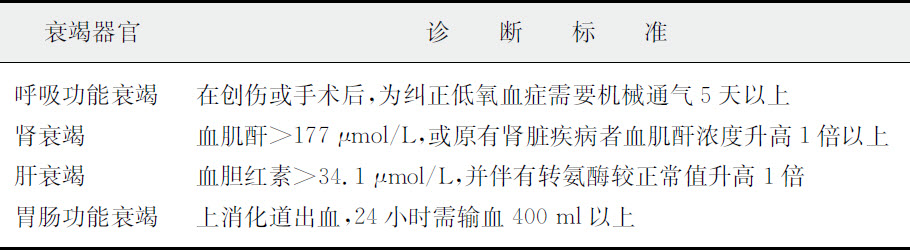
\includegraphics[width=5.91667in,height=3.44792in]{./images/Image00006.jpg}
\end{table}

\paragraph{三、急性肾盂肾炎}

本病多见于女性,尤其是生育年龄的妇女,而糖尿病患者及使用导尿管等装置的老年患者亦不少见。当患者有急起畏寒、发热,伴有腰痛、尿频、尿急、尿痛时,应考虑急性肾盂肾炎的可能。若尿常规检查证实有脓尿,则诊断大致可以成立。病原学的诊断有待细菌培养证实。若仅有高热而尿路症状不明显者,应与各种发热性疾病相鉴别。腹痛、腰痛明显者应与急性胆囊炎、阑尾炎、盆腔炎、肾周围脓肿等鉴别。一般经多次尿液检查即能诊断。B超或CT检查有助于胆囊炎和肾周脓肿的诊断。

\paragraph{四、急性胆道感染}

急性发热者伴有上腹绞痛时,应考虑急性胆道感染的可能,通过进一步检查诊断一般不困难(参见第78.1节)。老年患者由于疼痛的敏感性降低,可无胆绞痛的主诉,但胆囊区仍可有明显的压痛。本病应与急性病毒性肝炎、急性胰腺炎、左下肺炎、急性肾盂肾炎等疾病相鉴别。血清转氨酶及病毒性肝炎系列标志物、血和尿淀粉酶、X线胸片和尿液检查则有利于各自的诊断。B超、CT检查可发现胆系结石和梗阻。

\paragraph{五、细菌性肝脓肿}

寒战、高热、肝区痛或右上腹痛,体检肝大并有压痛或(及)肝区叩击痛,血象白细胞总数及中性粒细胞增加,应考虑本病。B超有助诊断,必要时在B超引导下行肝穿刺抽出脓液可确立诊断。阿米巴肝脓肿临床上与细菌性肝脓肿相似,但阿米巴肝脓肿起病较慢、病程较长、慢性消耗表现较常见,而高热及白细胞增多则较不明显,部分病例有痢疾史或证实有阿米巴肠病。B超引导下肝脓肿穿刺,典型阿米巴肝脓肿脓液为巧克力样,在抽脓最后部分近脓腔壁的脓液有可能找到滋养体。近年,无论是细菌性肝脓肿还是阿米巴肝脓肿临床表现不典型病例增多,常发生漏诊,应提高警惕。肝脓肿还要与肝癌(特别是肝癌中心坏死液化合并感染)、肝囊肿或肝包囊虫病合并感染、右膈下脓肿等疾病鉴别(参见第106.2节及第106.3节)。

\paragraph{六、其他急性局灶性细菌感染}

此类疾病的共同特点是高热、畏寒或寒战,周围血象白细胞和中性粒细胞增多,并有局部症状和体征。

\subparagraph{(一)膈下脓肿}

通常并发于腹腔化脓性感染或腹腔手术后,尤其是急性阑尾炎、胃及十二指肠穿孔、胆囊切除术、脾切除术后等。肝脓肿亦可直接向右膈下组织蔓延。若有上述情况,患者又出现寒战、高热、白细胞总数和中性粒细胞增高,又未能找到其他感染灶时,应想到此病的可能。膈下脓肿以右侧多见,患者自觉患侧上腹部有显著搏动性疼痛,以深呼吸或体位转动时加重,患侧下胸部常有局部皮肤水肿并有压痛及叩击痛,听诊呼吸音减弱或消失。站立位X线检查可发现患侧膈肌上升活动受限,反应性胸膜炎,患侧膈下可见液平面或气泡。B超或CT检查可早期明确诊断。

\subparagraph{(二)肾周围炎或肾周脓肿}

患者常以畏寒、发热或寒战高热开始,伴有患侧肾区疼痛,并向同侧下腹及大腿内侧放射,脊肋角显著压痛及叩击痛。当此病早期未出现肾周围局部体征时易误诊为全身感染或急性肾盂肾炎,及时进行B超或CT检查可明确诊断。

\subparagraph{(三)其他局灶性感染}

化脓性中耳炎、化脓性扁桃体炎、化脓性关节炎、化脓性骨髓炎以及其他各部位的浅部化脓性感染(如疖、皮下急性蜂窝织炎等)或深部化脓性感染(如臀肌脓肿、脑脓肿等)均可引起急性高热,局灶性症状和体征可提示诊断。

\paragraph{七、败血症}

败血症(septicemia)是指病原菌及其毒素侵入血流所引起的临床综合征,是一种严重的血流感染。尽管目前对败血症的定义仍有争议,但疾病国际分类(ICD)仍采用败血症这一病名。当患者有原发感染灶,出现全身性脓毒症症状,并有多发性迁徙性脓肿时提示败血症。值得注意的是有时原发的感染病灶可能很轻微或已愈合。因此,临床上遇到不明原因的急性高热,伴有畏寒或寒战、出汗,全身中毒症状重,白细胞总数和中性粒细胞明显增高,而无特殊症状、体征及流行病学病史提示急性传染病时,应考虑败血症的可能。医院内感染败血症绝大多数见于有严重基础疾病如各种血液病、肝及肾衰竭、晚期恶性肿瘤,或医源性感染如各种导管的长期置留、透析疗法等,如患者出现不明原因发热或(及)病情恶化时应注意败血症的可能。阳性血培养是诊断败血症的重要依据,反复多次做血培养可获得较高的阳性率。

根据我国近年对败血症病原学分析的报道,我国败血症的病原体以金黄色葡萄球菌、大肠杆菌和其他肠道阴性杆菌为多见,但表皮葡萄球菌、铜绿假单胞菌及一些耐药菌败血症有增加趋势,厌氧菌及真菌败血症亦非罕见。不同病原菌所造成的败血症临床表现可有一定差异,兹分述如下:

\subparagraph{(一)需氧革兰氏阳性球菌败血症}

\hypertarget{text00014.htmlux5cux23CHP2-5-1-2-7-1-1}{}
1.金黄色葡萄球菌败血症

此病较常见,国内对各地共1000余例次败血症的病原学分析表明,金黄色葡萄球菌败血症所占比例高达20\%~30\%。临床急起发病,常先有畏寒或寒战,继而高热、头痛与出汗,多伴有恶心呕吐、腹泻、全身肌肉及关节疼痛,皮疹形态多样化,可有瘀点、荨麻疹、猩红热样皮疹及脓疱疹等。迁徙性化脓病灶是本病的特点,对病因诊断有重要意义。迁徙性病灶以四肢和躯干的多发性软组织脓肿、多发性肺脓肿、脓胸、肝脓肿、化脓性脑膜炎、骨髓炎等多见。本病并发心内膜炎者可高达8\%。临床若遇发热持续不退,体检发现有心脏病理杂音的出现,伴有进行性贫血、反复出现皮肤瘀点、内脏血管栓塞、血培养持续阳性,应考虑心内膜炎的存在,及时做超声心动图有助确诊。

金黄色葡萄球菌败血症的诊断一般不难,当存在原发性皮肤化脓性病灶或导管插管处红肿热痛,出现寒战、高热等中毒症状时,首先应考虑本病的可能。若同时伴有皮疹与迁徙病灶,则可能性更大。但临床上部分患者急起发热,病史不清,会造或诊断困难。如当胸片发现多发性迁徙肺脓肿者,此时易误诊为肺炎;胸片有片状模糊阴影者,易误诊为肺结核;少数患者白细胞计数较低,发热呈稽留热时,可误诊为伤寒。提高对本病的警惕和认识。早期多次血培养有助于及早做出诊断。

\hypertarget{text00014.htmlux5cux23CHP2-5-1-2-7-1-2}{}
2.表皮葡萄球菌败血症

近年来本病逐渐增多,目前约占败血症总数的10\%~15\%,且70\%为医院内感染。常见于体内异物留置或植入者(如静脉导管、人工关节、人工瓣膜、起搏器等)。由于表皮葡萄球菌为正常皮肤表面的细菌,血培养假阳性率高,因此,血培养阳性难以鉴别是否为污染所致。然而当患者发热不退,体内留有异物(如静脉导管)处局部皮肤红肿、压痛,或人工瓣膜患者出现新的杂音或多发性血栓形成等,都是感染的有力证据。另外,双份(身体左右侧静脉)血培养同时阳性意义更大。

\hypertarget{text00014.htmlux5cux23CHP2-5-1-2-7-1-3}{}
3.肠球菌败血症

本病发病率近年未有明显增多的趋势,77\%为医院内感染,占院内感染败血症的10\%左右。病原菌常来源于泌尿生殖道,亦易发生于消化道肿瘤及腹腔感染的患者,因此,对有上述病史的急性发热患者,尤其是院内感染,要考虑本病的可能。由于本病对多种抗菌药物耐药,故病情多危重。

\subparagraph{(二)需氧革兰氏阴性杆菌败血症}

约占败血症总数的40\%左右,其中,最常见为大肠杆菌败血症,其次为肺炎克雷伯杆菌、铜绿假单胞菌和其他肠杆菌败血症。病原菌常从泌尿生殖道、肠道(尤其是下消化道)或胆道入侵,多见于一般体质较差,伴有各种影响机体免疫功能的原发病。热型不一,以弛张热多见,少数患者可有体温不升、双峰热。40\%患者可发生休克,休克的特点是出现早且持续时间较长,严重患者可出现多脏器功能损害。多数患者白细胞增高,少数患者正常或减少但常有中性粒细胞左移现象。本病与金黄色葡萄球菌败血症在临床上虽然很相似,但原发灶不同,早期出现休克以及迁徙病灶较少见,有临床鉴别价值。

铜绿假单胞菌败血症通常继发于重度烧伤、白血病、淋巴瘤、各种恶性实体瘤以及气管切开、静脉导管、导尿等。临床表现较一般革兰氏阳性杆菌败血症凶险,可有较特征性中心坏死性皮疹。患者淡绿色尿(绿球蛋白)可作为铜绿假单胞菌败血症的诊断佐证。

\subparagraph{(三)细菌L型败血症}

细菌在体内多种因素影响下失去细胞壁变为L型,临床上常在应用抗生素后产生。细菌转变为L型后临床表现与原菌感染不同,其常见临床表现为发热波动难以控制,多呈弛张热(占80\%)。胸片示间质性肺炎但呼吸道症状轻微,尤其是感染性发热应用抗生素后一度有效,以后发热起伏波动,白细胞总数不高而有核左移和中毒颗粒者。临床上L型细菌以金黄色葡萄球菌多见,因此,在无法确定其类型的情况下,可选择对L型金葡菌有效的抗生素进行试验性治疗。多次高渗及等渗双份血培养均培养出L型细菌可助确诊。

\subparagraph{(四)厌氧菌败血症}

厌氧菌多从肠道肿瘤、发炎的憩室、女性生殖道、压疮、感染的胆道等处入侵血流,常发生于有严重基础病免疫功能低下的患者。厌氧菌多与需氧菌同时混合感染。对有上述情况,敏感抗生素治疗效果不佳甚至恶化的败血症患者,应考虑厌氧菌混合感染的可能,应加做厌氧菌特殊培养以助诊断。病变组织有脏而臭的分泌物、含气体、有假膜形成是诊断的佐证。

\subparagraph{(五)真菌败血症}

主要以念珠菌感染为主,近年来发病率明显增高,绝大部分为机体抵抗力低下的医院内感染,常见于长期接受广谱抗生素、糖皮质激素、免疫抑制剂或肿瘤化疗患者。因此,对具有上述易感因素,持续高热,经足量高效抗生素治疗96小时无效,尤其存在真菌感染灶(如口腔黏膜、皮肤)者应警惕本病的可能。血培养发现真菌可确诊,但阳性率不足50\%,且培养费时较长。因此,对高度怀疑本病者,选择广谱的抗真菌药物治疗症状改善,体温下降至正常者,亦为有力的佐证。

\paragraph{八、结核病}

发热为结核病最常见的全身性毒性症状,多数为长期低热,但当病灶急剧进展扩散时则可出现高热,呈稽留热或弛张热热型,可伴有畏寒,但很少寒战。临床上属此类型者有急性粟粒型结核,某些肺外结核如网状内皮系统结核(无反应结核病)、结核性脑膜炎、浸润型肺结核。

\subparagraph{(一)急性粟粒型结核(急性血行播散型肺结核)}

急性粟粒型结核来源于自体结核病灶,当机体免疫功能低下时加重和恶化,并从血流播散。本病发病急骤,持续高热为早期或突出症状,中毒症状严重,有时伴有乏力、畏寒等非特异症状。由于临床上肺部粟粒型结核多见,患者常伴有咳嗽、咳痰、气短等呼吸道症状。病程中可伴有轻度肝脾大。周围血象中多数有白细胞减少,少数有全血细胞减少。亦有少数病例白细胞明显增高呈类白血病反应。本病早期胸部X线表现不明显或阴性时,易误诊为伤寒、败血症或恶性血液病。但本病患者常有呼吸道症状如咳嗽、气促等症状,且血象无相对的淋巴细胞增多,肥达反应阴性,多次血培养伤寒杆菌阴性可与伤寒鉴别。反复多次血培养无致病菌生长,高效广谱抗生素治疗无效,可与败血症鉴别。全血细胞减少又伴有肝脾大者,易与白细胞不增高的急性白血病或恶性组织细胞病混淆。本病在发病第一、二周内,由于病变太小,在胸片上不易发现病灶。因此,对怀疑本病者,若一次胸片阴性,应定期复查或行胸部高分辨CT检查,可发现典型的两侧肺野内大小相等、从肺尖到肺底均匀一致的粟粒状致密影。结核菌素试验阳性对诊断有参考价值,但阴性不能否定结核,特别是老年人或免疫功能低下的患者。此外,眼底检查近半数成人病例,可发现脉络膜上有灰白色或黄色圆形小结节,对本病的诊断极有帮助。

\subparagraph{(二)无反应结核}

属特殊类型结核病,见于免疫力严重低下患者,其特点为:①全身中毒症状较重,持续高热,故又称之为结核性败血症;②呼吸道症状出现较晚;③肝、脾、淋巴结肿大多见且早期出现;④可并发粒细胞缺乏甚至全血细胞减少,亦可呈类白血病反应;⑤合并肺门淋巴结或纵隔阴影增大者可高达72\%。本病临床上易与风湿性疾病、败血症、伤寒病、血液病和恶性淋巴瘤混淆,定期复查胸片或胸部CT,痰、淋巴结穿刺物涂片检出抗酸菌有助确诊。

\paragraph{九、伤寒与副伤寒}

\subparagraph{1.伤寒}

发热是伤寒的早期症状,有时为唯一症状,因此是未明原因发热经常要考虑的疾病之一。凡发热持续一周以上原因未明者,需注意伤寒的可能。传统观点认为具有诊断参考价值的临床表现有:①热型早期呈梯形上升,极期呈稽留热型持续,后期呈弛张型缓解,病程多为3~4周;②伤寒毒血状态,表现为表情淡漠,无欲面容;③相对缓脉与重脉;④发病一周左右胸前、腹上区分批出现少数玫瑰疹;⑤脾轻度肿大;⑥白细胞总数减少,相对淋巴细胞增多,嗜酸性粒细胞减少或消失。

近年来,我国伤寒的发病率已明显降低,其流行高峰亦已较为平坦,并发症已显著减少,且由于起病早期多已接受过抗菌药物治疗而致临床表现多不典型。因此,依靠流行病学资料和典型临床表现作出伤寒的临床诊断往往有困难,关键是要注意伤寒的可能。确诊主要靠病原学和血清学检查:①一周后肥达反应“O”抗体凝集效价≥1∶80,H抗体凝集效价≥1∶160,有诊断参考价值,病程中效价逐渐升高意义更大。但血清学诊断需密切结合临床,凝集效价持续阴性,不能作为否定伤寒的依据。②血、骨髓培养伤寒杆菌阳性是确诊的依据,尿、粪培养阳性可弥补血、骨髓培养的不足。

临床上对高度怀疑伤寒患者,亦可试用氟喹诺酮类、氯霉素、氨苄西林等进行诊断性治疗。用药后本病多在3~5日内体温逐渐下降,临床症状亦迅速好转。

\subparagraph{2.副伤寒}

流行病学特点与伤寒相同,但发病率远较伤寒低。副伤寒甲、乙临床表现难与伤寒鉴别,但副伤寒潜伏期较短,急性起病较多,早期胃肠炎症状较明显,热型不如伤寒典型。副伤寒丙可表现为轻型伤寒,急性胃肠炎或脓毒症。与伤寒相同,确诊有赖于病原学及血清学检查,但要注意副伤寒丙的血清凝集效价较低,少数患者可始终阴性。

\hypertarget{text00014.htmlux5cux23CHP2-5-1-2-10}{}
十、细菌性心包炎

结核性或化脓性心包炎:早期症状不典型,诊断较困难。因此,对不明原因的发热兼有心前区疼痛的患者,应想到本病的可能。体检发现心尖搏动弱,心脏扩大,心音遥远,应考虑本病。若心前区闻及心包摩擦音,可作出初步临床诊断。本病的心前区痛与急性心肌梗死疼痛类似,应注意鉴别。心电图、胸部X线有助诊断,心脏B超和心包穿刺可确诊。

\hypertarget{text00014.htmlux5cux23CHP2-5-1-2-11}{}
十一、兔热病

本病是土拉杆菌所致的急性传染病,属自然疫源性疾病,在我国见于西藏、青海、内蒙古、黑龙江及山东等地。主要传染源是野兔,其次是鼠类和羊。由直接接触,烹食未熟受染的野兔、松鼠及其他啮齿类动物,或被壁虱叮咬而受染。潜伏期一般为3~4日,起病大多急骤,高热伴寒战及毒血症状如头痛、肌肉酸痛,局部皮肤出现丘疹,继而化脓,坏死中心脱落而形成溃疡,边缘隆起有硬结感,伴有一定程度的疼痛。白细胞总数多正常,偶有轻度升高。土拉杆菌抗原皮内试验或荧光抗体试验有助于早期诊断。

兔热病分溃疡型和腺型、肺型、胃肠型、伤寒型或中毒型、眼腺型、咽腺型等不同类型。确诊有赖于血或病灶分泌物的细菌分离(特殊培养或动物接种)及阳性免疫反应。

本病应与鼠疫、炭疽、鼠咬热等的皮肤病灶和腺肿鉴别。尚应与各种肺炎、伤寒、结核、布鲁菌病、类鼻疽、组织胞浆菌病等相鉴别。

\hypertarget{text00014.htmlux5cux23CHP2-5-1-2-12}{}
十二、人感染猪链球菌病

猪链球菌病是由多种不同群的致病性链球菌引起的一种人畜共患传染性疾病,人感染猪链球菌并引起发病的情况比较少见,其传染源主要为猪链球菌感染的病猪和带菌猪,高危人群为屠宰、饲养生猪或加工、销售、运送猪肉类的人员,感染途径主要通过接触病死猪时致病菌经破损皮肤和黏膜侵入人体,或吃了未完全煮熟的病猪肉或内脏而感染,目前尚未发现人与人之间的传播。

人感染猪链球菌病潜伏期短,平均2~3天,可短至数小时,最长达7天。临床上可分为四种类型:普通型、休克型、脑膜炎型和混合型。起病急,临床表现为畏寒、发热、头痛、头昏等全身中毒症状。重症病例迅速进展为中毒性休克综合征,出现皮肤出血点、瘀点、瘀斑,血压下降,脉压差缩小;可表现出凝血功能障碍、肝、肾功能不全、急性呼吸窘迫综合征、软组织坏死,筋膜炎等。部分病例表现为脑膜炎,恶心、呕吐、昏迷,脑膜刺激征阳性,脑脊液呈化脓性改变。还有少数病例为混合型,即在中毒性休克综合征基础上,出现化脓性脑膜炎表现。部分病例在恢复期出现听力减弱、障碍。实验室检查外周血白细胞计数升高(严重患者发病初期白细胞可以降低或正常),中性粒细胞比例升高。诊断上结合疫情资料、流行病学调查资料和患者的发病情况、临床症状及早期病例的尸检报告可做出初步诊断;进一步的确诊有赖于实验室病原学诊断。

\protect\hypertarget{text00015.html}{}{}

\subsubsection{1.1.3 钩端螺旋体病}

鼠和猪是本病的主要传染源,其带有钩端螺旋体的尿可以污染各种水源,人与污染的水源接触,钩端螺旋体通过暴露部位的皮肤进入人体而造成感染。全国各地均有本病报道,但以南方各省多见。本病具有如下流行病学特点:①疫水接触史,患者在起病3~20天内到过鼠类出没或猪尿污染的污水沟、稻田,皮肤曾与污水接触。散发病例,因很多场所被污染,有时无明确接触史而常被误诊。②主要流行于夏秋收割季节,有时可在洪水过后造成流行。③患者多为青壮年农民、饲养员,外地进入疫区者亦易患病。本病临床表现复杂,临床表现轻重不一,轻者似感冒,仅表现为轻度发热。典型的临床特点为:早期有高热,全身酸痛,结膜充血,腓肠肌压痛及浅表淋巴结肿大等类似败血症的表现。中期为肝、肾、肺等多器官损害与功能紊乱。

本病可分为流感伤寒型、肺出血型、黄疸出血型、肾衰竭型和脑膜炎型。流感伤寒型多数以全身症状为特征,起病急骤,畏寒发热,头痛、全身肌痛并有鼻塞、咽痛、咳嗽等,而无黄疸和中枢神经系统症状,肺亦无明显病变,易误诊为流行性感冒、上呼吸道感染。但本病患者往往同时或随之出现肝、肾功能损害,半数有皮肤黏膜出血,不支持流感和上呼吸道感染。仔细调查流行病史有助于鉴别诊断。肺出血型应与肺结核、支气管扩张、肺肿瘤鉴别。通过胸部X线或CT等检查加以区别。黄疸型易误诊为黄疸型肝炎,但后者以纳差为主,无眼结合膜充血和腓肠肌压痛,ALT、AST明显升高,而CPK不高,病毒性肝炎系列标志物和流行病学史可资鉴别。肾衰竭型与流行性出血热临床表现有相似之处,但后者通常有酒醉貌,无腓肠肌压痛,流行性出血热特异性抗体和病毒抗原检查有助于两者鉴别。脑膜脑炎型的钩端螺旋体病与乙脑都在夏秋季流行,但后者无全身酸痛、结膜充血和腓肠肌压痛,且乙脑抽搐、昏迷等脑部症状较钩端螺旋体病明显,尿常规、肝功能多正常。

对于钩端螺旋体病的病原学诊断,应用暗视野显微镜可直接检查患者血、尿及脑脊液等标本中的钩端螺旋体。病原体分离可用体液培养或动物接种技术。血清补体结合试验和凝集溶解试验自病程第一周末开始升高,在第三、四周达高峰,间隔两周双份血清,效价增高4倍以上有诊断价值。酶联免疫吸附试验比凝溶试验阳性出现更早和更灵敏,有早期诊断价值。

\protect\hypertarget{text00016.html}{}{}

\subsubsection{1.1.4 立克次体感染}

\paragraph{一、斑疹伤寒}

流行性斑疹伤寒在我国已基本得到控制;地方性斑疹伤寒由鼠蚤传播,属自然疫源性疾病,国内以河南、河北、山东和辽宁等地报道的病例较多,以夏秋收割季节发生较多。本病以高热、剧烈头痛、全身肌痛起病,眼结膜充血,可有中枢神经系统临床表现。早期病例需与流感、流行性出血热、钩端螺旋体病、伤寒、恙虫病、流行性脑脊膜炎、大叶性肺炎等疾病鉴别。一旦典型皮疹出现(一般在4~6天内),则病象相当明显,参见第2.1节。

\paragraph{二、恙虫病}

恙虫病流行于夏秋季,患者在疫区的田野或草地上工作、卧息时,可因被受染恙螨叮咬而感染。流行季节有不明原因急性发热患者,要警惕本病的可能。须追查流行病学史与细致搜寻焦痂,参见第2.1节。

\protect\hypertarget{text00017.html}{}{}

\subsubsection{1.1.5 寄生虫感染}

\paragraph{一、疟 疾}

间日疟和三日疟具有间歇性、规律性、发作性寒战、高热和大汗,伴有贫血和肝脾大等典型的临床表现,诊断不难。而恶性疟疾的临床症状较复杂而多样化,发热前寒战较少,热型多不规则,热后较少出汗。伴头痛、肌痛、纳差等症状,常有恶心、呕吐、腹泻等消化道症状。高热患者常有剧烈头痛,并出现谵妄、抽搐和昏迷,脑膜刺激征明显(脑型疟疾),易误诊为乙型脑炎。部分恶性疟患者有相对缓脉,加之有脾大和白细胞减少,易与伤寒相混淆。因此,在到过疟疾流行地区后出现不明原因的发热,应警惕疟疾的可能。疟原虫的发现是诊断疟疾的主要依据,一次血片检查阴性不能否定,应在发作过程中反复检验。在发热前的畏寒期采血作厚滴片检查,可提高阳性率。血片阴性时可作骨髓涂片检查,其阳性率较血片为高。氯喹或奎宁对疟疾治疗有特效,一般用药后1~2天体温下降,症状基本控制,对高度疑似的病例可用常规剂量作诊断性治疗。

\paragraph{二、阿米巴肝脓肿}

见前述及参见第106.3节。

\paragraph{三、急性血吸虫病}

本病多发生于夏秋季,有严格的地区性,多见于初次接触疫水感染者,但慢性血吸虫患者在再次大量感染后亦可表现为急性感染。平均潜伏期40日左右,其间可出现疫水接触处皮肤发痒,红色小丘疹约1~2日消失。急性患者都有发热,发热的高低、热型、热程与感染轻重因个体反应不同而异。可高热持续不退,伴精神萎靡、意识淡漠,重听、腹胀、可有相对缓脉而误诊为伤寒,但白细胞总数增高及分类中嗜酸性粒细胞增多(一般占20\%~40\%),据此可与伤寒鉴别。急性血吸虫患者有肝大,伴不同程度压痛,以左叶为著,与肝脓肿相似,但B超、CT发现占位病变可资区别。血吸虫卵所造成的异位肺损害,除有呼吸道症状外,胸片常示两肺中下野、大小略不等粟粒点状影应与粟粒型结核相鉴别。肠道症状表现为腹泻、腹痛、黏液血便,部分患者可出现腹膜刺激征,腹部饱满,有柔软感和压痛,类似结核性腹膜炎。凡夏秋季接触疫水,病初出现尾蚴皮炎,具有发热、肝大伴压痛、腹痛腹泻,而血中嗜酸性粒细胞明显增高者,需考虑急性血吸虫病的诊断。但不典型和重笃病例可不出现嗜酸性粒细胞增高或反而减少,据此,亦不能完全否定急性血吸虫病的可能。下述检查有助于确立急性血吸虫病的诊断:

1.血清免疫学检查

(1)抗体检测:常用检测方法有环卵沉淀试验(COPT)、间接血凝试验(IHA)、酶联免疫吸附试验(ELISA)等。COPT法目前仍为疫区广泛应用。近年来建立的简便快速的ELISA方法、敏感度达90\%以上,且敏感性和重现性好。但应注意抗体检测法不能区别既往感染与现症患者。

(2)抗原检测:可证实活动性感染。单克隆抗体斑点酶联法检测循环抗原敏感性和特异均较高,其临床应用尚在进一步研究中。

2.目前采用尼龙袋新鲜粪便集卵孵化法,提高了阳性率,为主要的检查方法。但一次阴性不能轻易除外本病,宜反复多次进行,以获得病原学的诊断。

3.直肠黏膜活组织检查,可提高检出虫卵的阳性率。

\paragraph{四、旋毛虫病}

猪为人体旋毛虫感染的主要传染源。本病发病前1~2周有生食或半生食含旋毛虫幼虫包囊的猪肉史,初期主要为肠炎症状,如腹痛、腹泻和稀水便;急性期发热多在38~40℃之间,热型多为弛张热,也可呈不规则热,伴有肌肉疼痛和水肿、皮肤斑丘疹或猩红热皮疹等,血象白细胞和嗜酸性粒细胞增高,确诊有赖于胸大肌或腓肠肌肌肉活检找到梭形包囊和幼虫和(或)免疫学检查等。

\protect\hypertarget{text00018.html}{}{}

\subsubsection{附:丝虫病}

丝虫病系由丝虫寄生于淋巴组织、皮下组织或浆膜腔所致的传染病。淋巴丝虫病是由班氏、马来或帝汶丝虫寄生于淋巴组织所致的传染病。我国除山东、台湾为单纯班氏丝虫流行外,其余地区均有两种丝虫病流行。在丝虫病疫区,患者有发热、淋巴管(结)炎、阴囊内器官与组织炎症或象皮肿,血中嗜酸性粒细胞增多,须考虑丝虫病。

班氏丝虫寄生于深部或浅表淋巴结、淋巴管中,尤以腹腔、盆腔、腹膜后组织、肾盂、附睾、精索等部位为多。因此,除有肢体淋巴管炎外,尤以阴囊内器官与组织的炎症病变为多见,阻塞胸导管或乳糜池可致乳糜尿。马来丝虫主要寄生于人体四肢浅部淋巴系统,尤以下肢多见,因此,肢体淋巴管炎和象皮肿较明显,无乳糜尿及外生殖器局部病征,巨型象皮肿亦较少见。帝汶丝虫病主要表现为腹股沟、股及沿大隐静脉和其分支的淋巴管炎、淋巴结炎及膝部以下象皮肿。

丝虫病发热的特点是往往呈不规则的周期性发作,通常伴淋巴管、淋巴结炎。少数病例的淋巴管炎位于腹内深处,可无浅表病理体征。有些病例如阴囊内器官与组织炎症,在急性发作期疼痛可先从下腹部开始,或向腹部放射,故易误诊为阑尾炎或其他急腹症,但体检时腹部体征阴性而阴囊内有器官与组织炎症存在,可资鉴别。此外,精索与附睾炎要与附睾结核鉴别,后者结节在附睾内,常粘连在一起,不痛,少有反复发作。

病原学检查发现微丝蚴为确诊的直接证据。于晚间熟睡时采周围血作成厚涂片,每夜连续2~3次,检出率可达90\%以上。有实验条件者,采用间接荧光抗体或酶联免疫吸附试验可检测丝虫特异抗体。对疑似病例,服用乙胺嗪后肢体淋巴管或阴囊内出现新结节,或阴囊内原有病变增大、疼痛加剧,对丝虫病的诊断有一定的辅助诊断价值。

1994年,全国864个流行县、市(含班氏和马来丝虫病)全部达到基本消灭丝虫病标准,实现全国基本消灭丝虫病的目标。

\protect\hypertarget{text00019.html}{}{}

\subsection{1.2 非感染性急性发热疾病}

\subsubsection{一、风湿热}

风湿热是一种常见的反复发作的急性或慢性全身性结缔组织炎症,主要累及心肌、关节、中枢神经系统、皮肤和皮下组织。本病最常见于5~15岁的儿童和青少年,多数患者发病前1~5周先有咽炎或扁桃体炎等上呼吸道感染史。

风湿热患者多有低热,中等度热,亦可呈现高热。部分病例没有明显关节痛或关节炎的症状、以发热为主要临床表现,诊断有时困难。

迄今风湿热尚无特异性的诊断方法,主要依靠临床表现与动态观察,辅以实验室检查。临床上沿用修订的Jones诊断标准,认为具有下述2项主要表现或1项主要表现加2项次要表现,并先前有链球菌感染的证据,可诊断风湿热。

主要表现:①心脏炎:为临床上最重要的表现,其特征有:a.心肌炎,最早的临床表现为二尖瓣和主动脉瓣的器质性杂音。心尖区第一心音常减弱,常可闻及奔马律;b.心动过速,常>100次/分,与体温不成比例;c.心脏扩大;d.心律失常及心电图异常,常见为房室传导阻滞、期前收缩和心电图PR间期延长;e.心力衰竭,往往由急性心肌炎所致,尤其多见于年龄较小的患者;f.心包炎,出现于风湿热活动期,为严重心脏炎的表现之一。②多发性关节炎。③舞蹈病。④环形红斑。⑤皮下结节。

次要表现:①关节痛;②发热;③急性反应物改变(血沉降率增快,C反应蛋白增高);④心电图PR间期延长;⑤既往风湿热史和现患风心病。

有链球菌感染证据:①近期患过猩红热;②咽喉拭子培养或快速链球菌抗原试验阳性;③链球菌抗体效价升高。

在上述5项主要表现中,心脏炎和多发性关节炎的诊断意义最大。但亦非特异性。风湿热累及心肌时,表现为与发热不相称的心动过速和心电图异常改变,常有诊断参考价值。但由于也非特异性,亦需在鉴别的基础上考虑诊断。由于多关节炎的疾病种类繁多,多关节痛在几乎所有发热性疾病中经常可见,临床工作中,易将有类似表现的骨、关节和其他风湿性疾病如系统性红斑狼疮等误诊为风湿性关节炎,应予以重视。另一方面,约有1/4风湿热患者无多关节炎症状,甚至无关节痛,据此就不考虑风湿热的诊断,是另外一种错误倾向,应有所认识。风湿性心包炎的心包摩擦音,由于持续时间短暂,易被忽略而漏诊。主要表现中的后3项,发生率甚低,在诊断中起作用少。但少数患者尤其是儿童出现舞蹈病,结合某项其他表现,则有可靠的诊断价值。

上述的实验室检查是诊断风湿热的参考条件,但必须结合临床资料综合分析。抗“O”滴度>500U,认为有参考诊断价值,但不能作为确诊的依据。因为其阳性率仅有70\%~80\%,且仅表示新近有过链球菌感染,ESR在合并严重的心力衰竭时可以正常。部分风湿热患者白细胞计数增高。心电图有P-R间期延长、不完全性或完全性房室传导阻滞,多源性或多发性期前收缩、二联律、阵发性心动过速或房颤,QT间期延长有较大的参考诊断价值。但其心电图改变亦非经常出现,需定期反复复查才能发现异常,且上述心电图改变亦非风湿热特有。

1992年美国心脏病学会对Jones标准又进行了修订:该标准保留了Jones原5项主要表现,减去1项次要表现(既往风湿热史和现患风心病),并指出有下列3种情况时可不必严格执行该标准,即:①舞蹈病者;②隐匿发病或缓慢发展的心脏炎;③有风湿热病史或现患风心病,当再次感染A族链球菌有风湿热复发的高度危险性者。

患有风湿性心脏病患者有发热时,须考虑风湿性心内膜炎与亚急性细菌性心内膜炎两者的鉴别。后者多见于原有心瓣膜病,有进行性贫血、脾大、瘀点、瘀斑,可有脑、肾、肺等不同部位的栓塞症状。反复血培养阳性,超声心动图在瓣膜上发现赘生物可资鉴别。对已证实合并亚急性细菌性心内膜炎的风湿性心脏病患者,经足量抗生素治疗症状无改善或一度改善后又恶化,下列表现提示有风湿活动:①上呼吸道感染出现心悸、气促、病程超过半月以上者;②原因不明的难于纠正的进行性心力衰竭或急性肺水肿;③ESR增快,心力衰竭时ESR正常,心衰好转后ESR反而增快;④洋地黄治疗效果不好或耐受量降低易出现中毒症状;⑤不明原因的心律失常;⑥原有器质性心脏杂音性质的改变;⑦出现心脏以外的风湿性病变如风湿性脑病、脉管炎、关节炎、环形红斑等。此时做抗心肌抗体检测,心脏炎者阳性率达70\%,特异性高,抗A组链球菌胞壁多糖抗体(ASP)明显升高,阳性率达80\%以上,有助于判断风湿活动和其他心脏病鉴别。

如发热患者伴多关节炎、ESR增快,也可见于诸多结缔组织病、结核性关节炎或结核感染反应性关节炎、各种败血症引起的感染性关节炎或关节痛。此外,风湿热还要与SLE、成人Still病、莱姆病(Lyme病)、急性白血病,链球菌感染后状态等鉴别。

近年来风湿热、风湿性关节炎已明显减少,典型病例已不多见。但轻症、不典型病例仍可见到,给诊断带来一定的困难。

\subsubsection{二、系统性红斑狼疮}

部分系统性红斑狼疮早期可仅以发热为突出症状,其他系统受累的症状和体征可以不明显,诊断有一定困难。未明原因的无菌性急性发热,尤其是生育年龄的妇女,应考虑到本病的可能,并作进一步相关检查,参见第5.3节。

\subsubsection{三、急性白血病}

临床上凡患者急起发热兼有进行性贫血及(或)出血倾向,须考虑急性白血病的可能性。典型的急性白血病有持续发热、出汗、衰弱、出血倾向、进行性贫血、胸骨压痛,肝、脾及(或)淋巴结肿大,周围血细胞高度增多(也可正常或减少),以原始白细胞占优势,血培养阴性等表现。根据血象与骨髓象通常不难作出诊断。有的病例须与类白血病反应相区别,参见第5.2节。

\subsubsection{四、热射病}

热射病(包括日射病)亦称中暑性高热。表现为高热(>40℃)和神志障碍。本病基本上发生于高温季节,临床上可分为两种类型:劳力性和非劳力性(或典型性)。前者主要是在高温环境下内源性产热过多;后者主要在高温环境下体温调节障碍引起散热减少。

\paragraph{1.劳力性}

其特点是在高温环境和无风天气下进行体力劳动或剧烈运动时发病,多见于平素健康的年轻人。早期有头痛、乏力、恶心、口渴、心烦、少汗或多汗等非特异症状,继而急骤发病,体温急剧升高至40℃以上,皮肤灼热干燥,心率可达160~180次/分。脉压增大,可发生谵妄、抽搐、昏迷、出现病理神经反射。此种患者可发生横纹肌溶解和多器官功能衰竭,甚至死亡。

\paragraph{2.非劳力性}

在高温环境下,多见于居住拥挤和通风不良的城市老年人、产妇、体弱或患慢性病者。表现为皮肤干热、发红、无汗。病初可有各种行为异常和癫痫发作,继而可发生谵妄、昏迷、瞳孔对称缩小,终末期散大,严重者可出现低血压、休克、心律失常及心力衰竭、肺水肿、脑水肿。

根据病史和体征,本病一般不难诊断。尤其患者有高温接触史,出现昏迷和体温过高时应考虑热射病的可能。在诊断本病前应与脑炎、脑膜炎、脑型疟疾、脓毒病、脑血管意外、产褥热、甲状腺危象、抗胆碱能药物中毒及其他急性感染性疾病相鉴别。

\subsubsection{五、药物热}

药物热是机体对药物的一种超敏反应。常与特异性体质有关。患者往往先有感染,在给药后7~10天出现发热,多为低热或中等度发热,也可表现为高热。药物热大多数伴有药物皮疹或荨麻疹、肌肉关节痛,但有少数病例仅表现为发热,无皮疹及其他症状,一般情况好。药物热一般在停药后48小时内热退。再用该药,则在数小时内再次引起发热。药物热应与感染性疾病感染未能控制及风湿性疾病、肿瘤引起的发热相鉴别。

\subsubsection{六、恶性高热}

恶性高热是使用全身麻醉剂产生的严重并发症。麻醉剂以肌肉松弛剂和吸入性麻醉剂合用时发生率更高。家族性遗传性体质缺陷是内在的重要因素,其中以遗传性肌病更为重要。本病常在麻醉后立即发生,心律不齐是早期表现,常伴呼吸困难、发绀,常伴全身骨骼肌强直。高热或特高热是必有的主要症状,可高达40℃以上。高热期间血清肌酸磷酸激酶、丙氨酸基转移酶、乳酸脱氢酶增高,还可出现肌红蛋白血症,尿中出现肌红蛋白。常因心力衰竭、脑水肿、急性肾功能衰竭而死亡。诱发恶性高热的药物有琥珀酸胆碱、氟烷、乙醚、环丙烷、氯仿、甲氧氟烷、氯胺酮、氨氟醚等。

本病应与甲状腺功能亢进危象、嗜铬细胞瘤及恶性综合征等相区别。恶性综合征是抗精神病药物治疗特有而罕见的严重反应,主要表现为持续高热、肌肉僵硬、意识障碍及心血管症状等,可导致死亡。

\subsubsection{七、组织坏死性淋巴结炎}

组织坏死性淋巴结炎又称Kikuchi病,1972年由日本人首先报道,是一种主要累及淋巴结的良性、自限性、全身性疾病,误诊率较高,可达30\%~40\%。本病好发于青年女性,近年发病率有上升趋势,多累及颈部淋巴结,也可多部位先后出现淋巴结肿大,直径多在0.5~2.5cm;肿大淋巴结活动、无粘连,伴疼痛或压痛;发病前多有类感冒症状,体温38~39.8℃,抗生素治疗无效;实验室检查发现外周血白细胞计数在正常范围内或降低,血沉升高,PPD试验阴性。活检淋巴结破碎是特征之一。本病糖皮质激素有效是其特点,自然病程1~4个月。

\protect\hypertarget{text00020.html}{}{}

\subsection{1.3 急性“未明热”}

有少数急性发热患者未能查明原因,这些急性“未明热”以夏、秋二季为多见,且多见于年轻人。这些患者有急性感染的全身症状、体检及实验室检查无异常发现,病程通常在一周左右,预后良好。但是“未明热”仅为少数,有些病例由于检查未能周详及受设备条件或目前的认识所限,一时未能作出病因诊断,故诊断要慎重。必须除外引起急性发热的器质性疾病,首先要考虑病毒感染,其次为细菌感染如顿挫型伤寒、潜在的肺外结核、某些隐蔽的肿瘤等均要仔细排除。

\protect\hypertarget{text00021.html}{}{}

\section{2 急性发疹性发热}

在临床工作中,皮疹是常见的体征,据统计有100多种疾病发热伴有皮疹,常见有急性发疹性传染病、结缔组织病、变态反应性疾病、血液病等。一些原因不明的发热性疾病亦可发生皮疹,由于在不同疾病,皮疹可有不同形状,发疹时间及伴随症状也不相同。因此,可作为不同疾病鉴别诊断的一个重要体征(表\ref{tab2-3})。

\begin{table}[htbp]
\centering
\caption{急性发疹性发热性疾病的分类}
\label{tab2-3}
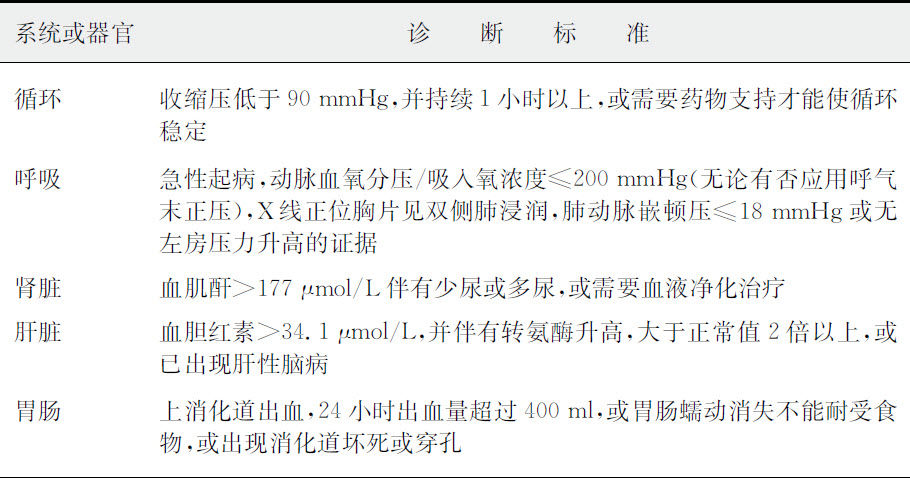
\includegraphics[width=5.9375in,height=1.84375in]{./images/Image00007.jpg}
\end{table}

\subsection{2.1 急性发疹性传染病}

急性发疹性传染病均有一定的潜伏期,掌握出疹的时间及其与发热的关系、出疹的部位及顺序、皮疹的性质及其相关体征、病程的经过,在鉴别诊断中有重要意义。

\subsubsection{一、麻 疹}

多在冬春二季流行,以儿童为多见。潜伏期为7~14天,发热3~5日出疹,主要症状有发热及上呼吸道卡他症状,同时有眼结膜充血、流泪、畏光日渐加重的表现,在发病第2~3日又可于双侧近臼齿颊黏膜处出现细砂样灰白色小点,绕以红晕,称麻疹黏膜斑,为本病早期特征。起病3~5日后,全身症状及上呼吸道症状加重,体温再度升高可达40℃,皮疹先于耳后发际出现,然后迅速发展到面部,自上而下蔓延直至手心足底;皮疹为淡红色、散在,然后密集呈鲜红色,持续约5日左右。皮疹出齐后按出疹顺序隐退、脱屑、色素沉着、整个病程10~14日。上述皮疹的临床表现,结合流行病史,血象白细胞计数正常或减少,80\%~90\%患者鼻咽、眼分泌物涂片染色镜检可发现脱落的上皮多核巨细胞、并可寻找到特异性麻疹抗原可诊断。从上述分泌物或血液白细胞中分离到麻疹病毒则可确定诊断。

在近期接受过免疫抑制剂或接种过疫苗者,全身症状轻、皮疹散在、不留色素,甚至可无皮疹和口腔黏膜斑。出血性皮疹多见于免疫力低下的重型患者。

成人麻疹的临床表现与儿童大致相同,但一般中毒症状较重,并发症也不少,且以呼吸道并发症多见。

麻疹需与风疹、猩红热、药疹等相区别。

\subsubsection{二、风 疹}

潜伏期较长为14~21天左右,主要发生于儿童,亦可见于青少年。临床症状较麻疹轻,发热仅1~2天,起病后即有皮疹出现,分布于颜面部,迅速波及躯干部,皮疹呈现玫瑰色斑丘疹,可融合成片。体温随皮疹的出现而上升,但较少超过39℃,通常2~3天内退热。其重要体征为伴有耳后、枕部甚至全身淋巴结肿大,无压痛。与麻疹的皮疹不同的是,皮疹的消退和发展同样迅速,疹退时体温亦下降,肿大的淋巴结亦逐渐恢复。皮疹消退后一般不留色素沉着,亦不脱屑。

风疹早期白细胞总数减少,淋巴细胞增多,并出现异形淋巴细胞,浆细胞增多,特异性风疹抗体IgM阳性有诊断意义。

风疹患者的皮疹形态介于麻疹与猩红热之间,因此,应着重对此三种常见的发热性出疹性疾病进行鉴别诊断。流行病学资料对鉴别诊断有重要帮助。

\subsubsection{三、传染性红斑}

本病病原为B19病毒,发病多见于儿童,少数亦可见于成人。潜伏期为4~12天,皮疹在第1~2天出现,最初为颊部水性红斑。后为全身斑丘疹,呈环形、网状,常有痒感,四肢亦可出现对称性斑丘疹,但罕见于手掌和足底。往往能同时出现发热、上呼吸道症状、肌痛和胃肠道症状。血清或咽拭子检测到特异性IgM抗体可确立诊断。本病需与药物疹、风疹和猩红热相鉴别。

\subsubsection{四、水 痘}

水痘是由于水痘带状疱疹病毒引起的急性传染病,多见于小儿,其潜伏期为10~24天。皮疹常于发病数小时或1~2天内分批出现,往往同时出现发热、头痛、咽痛、四肢酸痛和胃肠道症状。皮疹先见于躯干,逐渐延及面部,最后达四肢。皮疹呈向心性分布,以躯干为多,面部及四肢较少。皮疹发展快为本病的特征之一,开始为粉红色帽针头大的斑疹,数小时内变为丘疹;再经数小时变为水疱。短者这一过程仅6~8小时。水痘初呈清澈水珠状,以后稍混浊,壁薄易破,疱疹在24小时内开始皱缩、结痂。痂皮脱落后遗留浅瘢痕。水痘典型病例诊断不难,必要时可作血清学补体结合试验,出疹后1~4日即出现补体结合抗体阳性,可协助诊断。近年应用PCR方法检测鼻咽部分泌物VZVDNA,为敏感和快速的早期诊断手段。

水痘主要与轻症天花相鉴别,其鉴别要点如表\ref{tab2-4}。

\begin{table}[htbp]
\centering
\caption{水痘与天花的鉴别诊断}
\label{tab2-4}
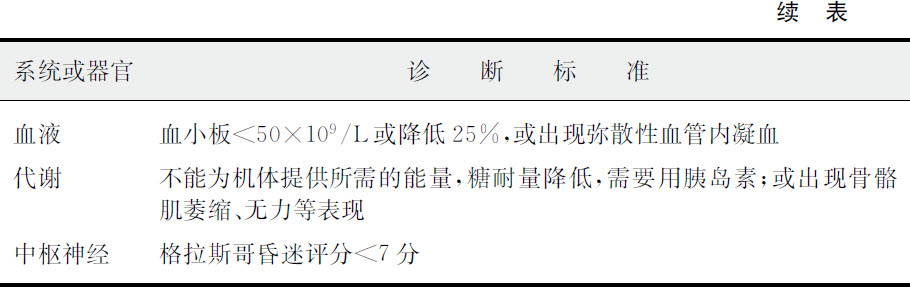
\includegraphics[width=6.04167in,height=3.8125in]{./images/Image00008.jpg}
\end{table}

\subsubsection{五、登革热}

登革热为登革病毒引起,经蚊传播的急性传染病,多流行于夏秋季节。潜伏期2~15日。其临床特征为双相热、剧烈头痛、皮疹、肌肉骨关节剧烈酸痛、淋巴结肿大、白细胞和血小板减少、淋巴细胞相对增多。

本病多数起病急骤,常以畏寒发热开始,颜面及眼结膜显著充血,颈及上胸皮肤潮红,发热持续2~4天即退,皮疹常于发病后2~5天出现。初见于掌心、脚底或先发生于躯干及腹部。然后蔓延至全身。皮疹呈麻疹样,少数呈猩红热样,或介于两者之间,压之褪色。体温下降者此时又可再次上升(呈马鞍热)。皮疹于1~5日(平均3日)消失,体温同时下降。整个病程约5~7日。本病确诊有赖于病毒分离。目前国内用酶联免疫吸附试验检测特异性IgM抗体,对早期诊断有较大的意义。PCR方法检测登革热病毒RNA,具有快速、敏感性高、特异性强的优点。

\subsubsection{六、斑疹伤寒}

斑疹伤寒可分为流行性斑疹伤寒和地方性斑疹伤寒,两者临床特征相近似,但后者病情较轻,病程亦较短,皮疹很少呈出血性。

典型的斑疹伤寒,流行于冬春季节,其潜伏期为5~21天,常急骤起病,体温于第2~4天即达高峰(39~40℃),呈稽留高热型,伴有速脉(与体温升高程度呈正比)、头痛、周身肌肉痛、眼结膜及脸部充血。皮疹于病程第4~6日出现,为本病重要体征,见于80\%以上病例。初见于胸背、腋窝、上臂两侧,1日内迅速波及全身。而面部及下肢皮疹较少。但可出现于手心和足底,皮疹初为鲜红色,继而转为暗红或瘀点状。神经系统症状明显且出现早,头痛、呆滞、神志迟钝,加之患者有脾大,酷似伤寒。但本病一般无相对缓脉,血、粪培养阳性可资区别。部分流行性斑疹伤寒有腓肠肌压痛、肝大、黄疸和肾损害,少数伴有出血皮疹,在南方地区易与钩端螺旋体病混淆。但后者有疫水接触史,有全身出血倾向,皮肤出血而非呈斑丘疹状,白细胞增高,ESR增快,血清凝溶试验阳性可资鉴别。

流行性斑疹伤寒的诊断有赖于血清学检查:①外斐试验其凝集效价>1∶320,有参考诊断价值,因为非立克次体病变等也可出现阳性反应,但效价较低。复发型斑疹伤寒外斐试验往往阴性或效价<1∶160,故有鉴别诊断价值。②以提纯的普氏立克次体颗粒性抗原作补体结合试验,不仅具群特异性,且具种特异性,可区别流行性斑疹伤寒和地方性斑疹伤寒。③以可溶性抗原作立克次体凝集试验,特异性高,操作简便,可用于与其他群立克次体区别。且流行性斑疹伤寒的凝集抗体为IgM,复发型斑疹伤寒为IgG,两者可作鉴别。④分子生物学检查,用DNA探针或PCR方法检测普氏立克次体特异性DNA,具快速、特异、灵敏等优点,但作为诊断依据时,仍需结合临床表现和流行病学资料作出判断。

流行性斑疹伤寒与地方性斑疹伤寒的鉴别见表\ref{tab2-5}。

\begin{table}[htbp]
\centering
\caption{流行性斑疹伤寒与地方性斑疹伤寒的鉴别}
\label{tab2-5}
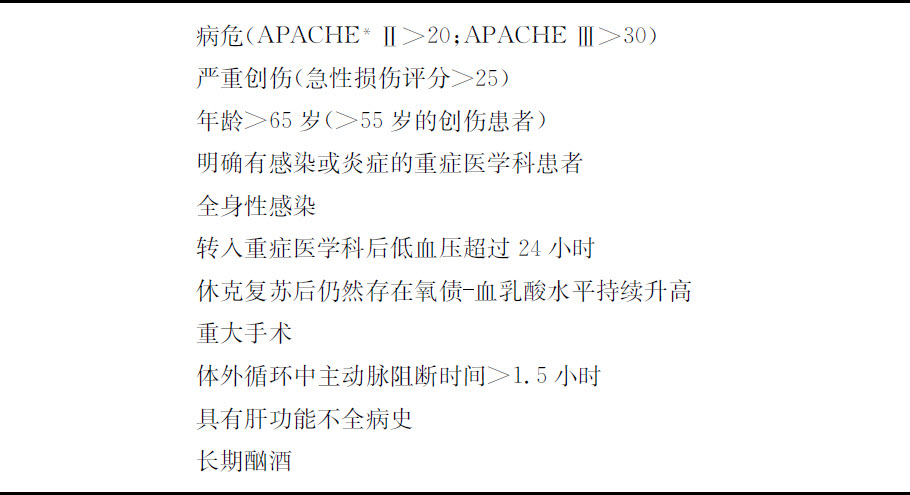
\includegraphics[width=5.94792in,height=1.67708in]{./images/Image00009.jpg}
\end{table}

斑疹伤寒还应与伤寒、回归热、流行性脑膜炎,流行性出血热、恙虫病、麻疹等鉴别。依据流行病学史及相关的实验室检查,一般可作出鉴别诊断,与伤寒的鉴别见表\ref{tab2-6}。

\begin{table}[htbp]
\centering
\caption{斑疹伤寒与伤寒的鉴别}
\label{tab2-6}
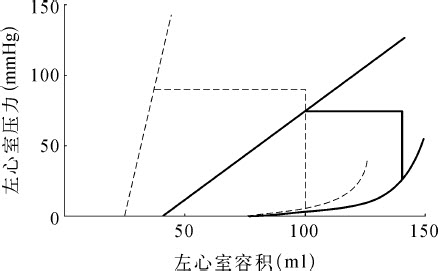
\includegraphics[width=5.95833in,height=3.45833in]{./images/Image00010.jpg}
\end{table}

\subsubsection{七、恙虫病}

恙虫病的潜伏期为5~20日,流行于夏秋季节,农民、与草地接触频繁的青少年及从事野外劳动者易得此病。起病多突然、体温迅速上升,达39~40℃,伴寒战、头痛、四肢酸痛、颜面潮红、结膜充血,类似斑疹伤寒的面容。严重者有谵妄、重听、腹胀、神志改变,部分患者可发生肠出血,易误诊为伤寒。焦痂和溃疡为本病的特殊体征,见于65\%~98\%患者。焦痂多见于腋窝、腹股沟、会阴、外生殖器、肛门等处。幼虫叮咬处出现红色丘疹,成水疱后破裂,中央坏死,结痂呈褐色或黑色,痂皮脱落后成小溃疡,边缘略隆起,底部为淡红色肉芽肿。因焦痂与溃疡无痒痛,发生于隐蔽部位,易被忽略。但仔细体检,往往可发现焦痂或溃疡,其附近的淋巴结肿大疼痛,有助于本病的诊断。

皮疹的发生率自30\%~100\%不等,为斑疹或斑丘疹,暗红色,压之即退色。皮疹多见于胸背和腹部,向四肢发展,面部很少,手掌脚底无疹,此点有助于与斑疹伤寒的鉴别。

血清免疫学检查:①外斐试验:患者血清可与变形杆菌oxk株发生凝集反应,阳性率70\%~80\%,滴度递升有诊断价值;②补体结合试验,特异性和敏感性较外斐试验高。

分子生物学检查:PCR检测恙虫病立克次体Sta58或Sta56抗原基因片段的方法诊断价值更高。

\subsubsection{八、猫抓病}

本病是汉赛巴通体经猫抓、咬人体后侵入而引起的传染病。主要临床表现为被猫抓咬后3~10日,局部出现红斑性丘疹,少数丘疹转为水疱或脓疱,少数可穿破形成小溃疡,可留下短暂色素沉着或结痂而愈。体检可发现抓伤感染部位引流区域淋巴结肿大。全身症较轻,半数患者有发热(>38.3℃)及出现胃肠道症状、头痛和结膜炎。结膜炎可伴耳前淋巴结肿大为本病重要体征之一。

本病病变部位的焦痂与溃疡须与恙虫病鉴别,后者的临床症状重,并发症多,焦痂和溃疡多在隐蔽部位,血白细胞增高,流行病学史有助于鉴别。

本病确诊有赖于淋巴结或皮损处的活检涂片中发现汉赛巴通体。

\subsubsection{九、猩红热}

猩红热是乙型溶血性链球菌引起的急性传染病,流行于冬春两季,早期软腭上有小米粒状红疹或出血点,常在皮疹出现之前出现,可提示早期诊断。典型病例以寒战高热起病,伴咽峡炎。患者于起病第2天出现弥漫充血基础上的点状(针尖大小)猩红色斑疹,自胸上部与颈底部开始,继而波及全身,严重者皮疹可为出血性,有瘙痒感。皮疹以躯干、皮肤皱褶处、大腿内侧为多,面部仅有发红而无皮疹,唇周反现苍白,即所谓猩红热面容,皮疹消退后,有大片脱皮现象,如见于病程后期亦有诊断价值。此外,患者有咽痛、杨梅舌等。血象白细胞增多,病程第一、二周后,可有嗜酸性粒细胞增多趋势。恢复期少数病例可并发肾炎与中毒性神经炎等。

猩红热无特异性的实验室检查:咽拭子培养可发现溶血性链球菌,但无特异性,阳性结果须结合临床考虑。皮疹消退试验:于皮疹处皮内注射猩红热抗毒素0.1ml或恢复期血清0.5ml,注射部位皮疹在6~8小时消退,有助猩红热的诊断。

猩红热须与风疹、麻疹、药疹、类猩红热鉴别(表\ref{tab2-7})。

\begin{table}[htbp]
\centering
\caption{猩红热、麻疹、风疹、药疹的鉴别}
\label{tab2-7}
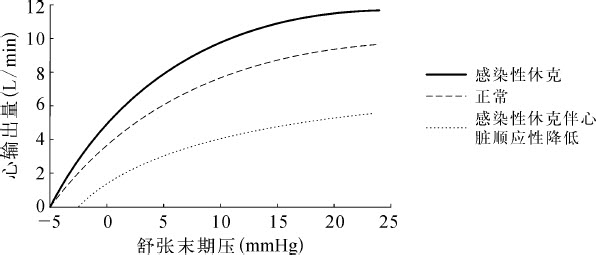
\includegraphics[width=5.97917in,height=3.92708in]{./images/Image00011.jpg}
\end{table}

\subsubsection{十、伤寒、副伤寒}

伤寒、副伤寒的皮疹为玫瑰疹,约20\%~40\%患者于病程第7~13日出疹。分批出现。副伤寒的玫瑰疹出现较伤寒早,有时数量较多,但玫瑰疹的发生率较少,且不典型,易被忽视,需注意与其他肠道革兰氏阴性杆菌败血症鉴别。确诊有赖于血、骨髓、粪便培养。肥达反应也有参考价值。

\subsubsection{十一、丹 毒}

丹毒是由β溶血性链球菌侵入后引起皮肤及其网状淋巴管的急性炎症。起病急、高热、寒战和全身不适。其皮肤病变好发于下肢和面部,局部烧灼样痛,片状红疹,中间较淡,边缘清,略隆起,有时形成水疱,内含浆液样液体。血象白细胞增高,分类左移。以水疱中抽取浆液样液体作涂片和培养,可发现溶血性链球菌,对确诊有重要价值。

丹毒需与急性蜂窝织炎区别,后者是皮筋膜下、肌间隙或深部蜂窝组织的急性弥漫性化脓性感染,炎症病变部位较深在,迅速扩散,边缘不隆起,界限不清,全身症状较明显,且有原发感染灶可寻。

发生于肢体的丹毒尚需与丝虫病淋巴管炎相区别。丹毒及其他细菌性淋巴管(结)炎,局部皮肤红肿疼痛剧烈,压痛明显,全身中毒症状明显。病灶发展呈向心性,远端皮肤有破损。通常不在同一部位反复发作,局部无硬结。丝虫病淋巴管(结)炎,局部淋巴结肿大疼痛,淋巴管肿胀从近端向远端扩展,晚期表现为淋巴管阻塞,炎症反复出现。若为班氏丝虫病,还可引起精索炎、附睾丸和睾丸炎。腹股沟处的淋巴结有硬结感。本病早期白细胞轻度增高,嗜酸性粒细胞显著增多。

丹毒还需与类丹毒相区别,类丹毒是由于感染猪丹毒的红斑丹毒丝菌引起。本病是一种职业病,主要由于与受污染的生肉(主要为猪肉)接触而发生感染。好发于屠宰工人和炊事员,外伤为诱因。病变多局限在接触的手与手指,虽然皮肤损害与丹毒相似,但与丹毒好发于下肢和面部不同。类丹毒颜色略呈青红,不起水疱,逐渐向周围发展。全身中毒症状不如丹毒明显。只有少数严重病例,皮疹波及全身时,才有发热。

\subsubsection{十二、兔热病}

兔热病绝大多数地区的主要传染源是野兔,其次是鼠类和羊。人类通过直接接触或吃了未煮熟的含菌兔肉或为鼠粪污染的食物和饮水而受染。皮肤感染局部形成红斑或丘疹,继而化脓坏死,中心脱落形成溃疡,边缘隆起而有硬结感。流行病学史,特别是有野兔接触史及相关职业等均有重要参考意义,确诊有赖于细菌分离和阳性免疫反应。

\subsubsection{十三、鼻 疽}

鼻疽是由马鼻伯克菌引起的感染性疾病,马科动物是主要传染源,患者发病前有与马直接和间接接触史。细菌从皮肤破损处进入,形成一个小结节,伴全身症状,急骤畏寒高热,病程进展,感染部位呈蜂窝织炎,进而有坏死的溃疡形成。当细菌从黏膜进入体内时,可引起眼、鼻和口腔感染继而出现溃疡和肉芽肿性病变。严重病例首先出现全身丘疹,随后发展为全身脓疱,侵入血液而形成败血症。

本病临床表现复杂,常不易确诊。必须结合接触病兽和实验室接触病菌史,分泌物涂片中荧光抗体阳性或各种培养物分离病菌,为主要诊断依据。血清学试验阳性有助于诊断。

本病须与类鼻疽、孢子丝菌病、链球菌蜂窝织炎和败血症鉴别。

类鼻疽是类鼻疽伯克菌引起的人畜共患的疾病,临床表现与鼻疽极为相似,局部化脓感染表现为皮肤破损处结节形成,引流区域淋巴结肿大和淋巴管炎,常伴畏寒发热和全身不适。急性肺部感染是类鼻疽最常见的类型,肺部炎症多见于上叶,呈实变,并常有薄壁空洞形成,易误诊为结核病。此型可发展为败血症。

病原学检查:以渗出物、脓液作染片和培养、悬滴试验可观察到动力,可以与马鼻疽伯克菌区别。尿中类鼻疽伯克菌抗原检测、胶乳凝集试验灵敏性较差,但特异性强;酶联免疫吸附试验灵敏性和特异均较高,可作为确诊的依据。

\subsubsection{十四、莱姆病(Lyme病)}

莱姆病是一种蜱媒螺旋体病,本病的传染源主要是野生和驯养的哺乳动物,啮齿动物中的白足鼠、哺乳动物中的鹿更为重要。当人的皮肤被蜱叮咬以后,出现慢性移行性红斑。开始时为一个红色斑疹或丘疹,然后逐渐扩大形成一片大的圆形皮损,外缘有鲜红边界,皮损早期中央有时呈致密红斑、硬变、疱疹、坏死。一般经2~3周皮损自行消退。50\%~80\%可并发多关节炎,11\%~15\%表现为神经系统广泛受累,表现为脑脊髓膜炎、颅神经炎、舞蹈病、小脑共济失调、脊髓炎等。且常先于关节症状出现,8\%~10\%患者有心脏受累(以房室传导受累多见、少数患者有房颤和心包炎),约10\%患者有肝炎样症状与体征。本病的多关节炎、舞蹈病需与风湿热鉴别。出现神经系统的并发症时,应与原发于神经系统本身的疾病区别。

本病的诊断主要依据流行病学资料与临床表现,慢性移行红斑具有重要诊断价值。血清学的诊断以酶联免疫吸附试验最为灵敏。特异性抗体效价>1∶200具诊断价值。血、脑脊液、皮肤活检标本培养阳性,则可确诊。

\protect\hypertarget{text00022.html}{}{}

\subsection{2.2 风湿性疾病}

\subsubsection{一、风湿热}

临床上约有1/3的风湿热患者在病程中有皮疹出现,具有诊断意义的为环形红斑和皮下结节。环形红斑少见,发生率为3\%~5\%,为淡红色红晕,中央苍白,不痛不痒,压之退色,多见于躯干和四肢近端,红斑初时较小,继而迅速向周围扩大,边缘略隆起,几个红斑融合可形成较大、不规则的圆圈,常为一过性,出现快,消失亦快。

皮下结节,亦少见,发生率不到2\%,结节多位于肘、膝、枕部、前额、棘突等骨质隆起或肌腱附着处,如豌豆大小,结节坚硬、无痛,与皮肤不粘连。

其他皮疹如荨麻疹、多形红斑、结节红斑等亦可见到,无特异性诊断价值。

\subsubsection{二、系统性红斑狼疮(SLE)}

约80\%~85\%SLE患者有皮疹,皮肤损害为多形性。颜面蝶形红斑,周围红斑和指(趾)甲远端下红斑具有特征性,常出现较早,前者是诊断本病的一个重要病征。其他皮肤损害有斑丘疹、水疱、大疱和血疱,日光暴晒后加重(光敏感)为本病的另一重要病征。有时可出现荨麻疹样损害。由于有部分SLE患者早期可无皮肤损害,而以发热或关节炎为首发症状,易误诊为败血症和风湿性关节炎。本病白细胞不高或减少,分类无左移可与败血症区别,SLE自身抗体,如抗核抗体(ANA)敏感性高达95\%,是SLE最佳的筛选试验,抗双链DNA抗体和抗Sm抗体特异性高,阳性有确诊价值。据此可与风湿性关节炎鉴别。

\subsubsection{三、急性皮肌炎}

本病较少见,皮肤和肌肉受累是导致本病的两组主要症状,皮损往往先于肌病发生。发热可为本病的初发症状,故早期诊断有一定困难,本病的皮疹为多形性,通常在面部尤其是上眼睑发生紫红色斑,逐渐向前额、颧、耳前、颈上胸部V字区扩展。闭眼近睑缘处可见明显扩张的枝状毛细血管,以眼睑为中心出现眶周水肿性红色斑片,具有一定的特征性,掌指关节和指间关节伸面出现红色丘疹、斑疹,以后萎缩、色素减退,上覆盖细小鳞屑,可见溃疡,称Gottron征,亦具特征性。肌肉往往四肢肌肉首先累及,近端重于远端,肩胛带和骨盆肌肉通常最早累及,上臂和股部肌群次之,其他部位肌群更次之。病变呈对称性。由于全身任何部位皆可受侵犯,故患者可出现肌肉疼痛,肌力下降,各种运动功能障碍和特殊姿态,如不能坐立,步态拙劣,伸展困难。面肌运动障碍,可出现张口受限,缺乏表情。

急性皮肌炎的免疫学检查可发现血清中肌浆球蛋白抗体,阳性率为90\%,其他结缔组织病此抗体阴性。血清肌酸磷酸激酶(CPK)、醛缩酶、AST、ALT、LDH均增高,且与肌肉病变的消退平行。上述血清肌浆酶的测定中,以CPK和醛缩酶最为敏感。借此可与SLE、类风湿关节炎、硬皮病鉴别。尿肌酸测定,皮肌炎患者24小时尿肌酸明显增多,甚至可高达2000mg。

急性皮肌炎患者的肌电图改变为肌原性萎缩相,见于90\%病例,据此可与其他神经肌肉疾病鉴别。

肌肉活检对皮肌炎的诊断有重要诊断价值。但非皮肌炎所特有,风湿性多肌痛症亦有轻度肌病性改变,但后者肌电图及CPK正常可资鉴别。

\subsubsection{四、成人Still病}

成人Still病(旧称变应性亚败血症),本病以间歇性发热、一过性多形皮疹、关节炎或关节痛、咽痛和周围血白细胞增高为主要表现的临床综合征。发热是最主要的症状,几乎见于所有病例,多呈弛张热型,通常在39~40℃以上,热退后如常人。皮疹在病程中皆可出现,可忽隐忽现亦可持续数小时,甚或几天。皮疹的出现可为发热的先兆,常随热退而消散。皮疹为多形性及多变性,可呈点状和小片红斑或斑丘疹,亦可表现猩红热样、麻疹样、荨麻疹样、多型红斑、环状红斑或结节红斑。关节症状主要累及大关节,但亦可侵犯小关节。表现为疼痛和压痛,但肿胀较轻且少。半数患者伴有全身淋巴结肿大和肝脾大,但热退时可随之缩小。白细胞总数增高,一般在(10~20)×10\textsuperscript{9}
/L,少数可高达50×10\textsuperscript{9}
/L,并有明显的核左移。骨髓检查常提示感染性骨髓象,肝功能亦有不同程度异常。ESR明显增快,不发热或间歇期亦然。血清铁蛋白亦明显增高。国内一组试验测定本病的铁蛋白平均为1194.5mg/L,活动期平均2742.9mg/L,其他风湿病平均为94mg/L。因此,可作为成人Still的诊断或活动的佐证。

成人Still病无特异性的诊断方法,主要依据临床表现和排除性的诊断。临床上凡有原因未明的发热,间歇热型、高热而中毒症轻,关节炎或关节痛,皮疹、白细胞增高,血清蛋白增高,血培养阴性,抗生素治疗无效而肾上腺皮质激素效果显著,则需考虑本病的可能。但须与下列疾病鉴别。

\paragraph{1.败血症}

中毒症状明显,发热前常有寒战,病程持续而非一过性和间歇性。肾上腺皮质激素疗效短暂,积极而合适的抗生素治疗有效,血培养阳性。白细胞总数和中性粒细胞增高时,嗜酸性粒细胞减少或消失。

\paragraph{2.风湿热}

有发热和关节症状,其皮疹主要为环形红斑和皮下结节。成人Still病皮疹大多为多形性。环形红斑极少见。二者虽可累及心脏,但风湿热心脏炎、心内膜炎、心包炎更为常见。抗“O”明显升高,而成人Still大多正常,血清铁蛋白亦两者皆可升高,但显著增高,则倾向于成人Still病的可能性大。

\paragraph{3.类风湿关节炎}

起病较隐匿,以侵犯四肢对称性小关节和晨僵为特点,少有高热和全身症状,类风湿因子阳性。不难与之区别。

\paragraph{4.系统性红斑狼疮(SLE)}

发热、关节痛、皮疹与成人Still病相似,但SLE皮疹以面部蝶形水肿性红斑为主,血象白细胞总数不高,抗核抗体阳性,抗ds-DNA抗体阳性,多系统损害较多见,据此可与SLE鉴别。

\paragraph{5.恶性淋巴瘤}

表现为长期高热者多,肝脾淋巴结呈进行性肿大,皮疹多为浸润性斑丘疹,结节、斑块和溃疡。淋巴结和皮肤组织活检有助于与成人Still病区别。

\paragraph{6.Sweet综合征}

本病又称“急性发热嗜中性粒细胞皮肤病”,具周期性发热、关节痛、皮疹及白细胞增高,与成人Still病极相似,但Sweet的皮疹为多发性、隆起不对称红斑性痛性皮肤斑块,皮肤组织学检查(以真皮层密集的嗜中性粒细胞浸润为特征)可确诊。

成人Still病的诊断必须十分慎重,一些败血症经抗生素治疗后血培养可以阴性,某些潜在的隐性感染有时难以发现,有些恶性淋巴瘤多次活检也可无异常发现,淋巴瘤对肾上腺皮质激素亦有短暂疗效。故诊断成人Still病必须进行排除性的诊断。

\subsubsection{五、结节性红斑}

本病的特征是小腿胫前皮下的红色或紫红色炎性结节。皮疹常突然发生伴有体温升高(39~40℃)及全身不适,多对称出现于小腿伸侧。少数可发生于小腿下1/3部及踝部,为皮下结节,稍高出于皮面或陷没于皮下。大小约1~5cm。质中等硬度,有显著疼痛和压痛,表面稍热、不化脓、不溃破成溃疡,结节上面的皮肤颜色初为红色,后渐变为暗红或青红与渗出性红斑、多形红斑相似,与后者不同之点是皮疹呈紫蓝色或较暗的棕蓝色。

结节性红斑可自行消退,遗留暂时性色素沉着。亦可反复发作,结节广泛。

结节性红斑应与硬结性红斑鉴别,后者起病缓慢,结节多出现于小腿内侧,通常3~5个。结节呈暗红色,核桃大小、质硬、不痛、易溃破形成溃疡。与结节性红斑不同,可资鉴别。

\protect\hypertarget{text00023.html}{}{}

\subsection{2.3 免疫性疾病}

\subsubsection{一、血清病}

血清病是由于注射动物免疫血清后所并发的一种免疫复合物性疾病。主要临床表现为皮疹、发热、关节痛、淋巴结肿大。症状的发生和程度与接种途径(皮下或静脉)、注射血清的剂量及过去有无同样接触史有关。初次一次性注射较大剂量异种血清引起的血清病症状出现在1~3周。少数患者尤其是过去有过同样血清接触史者,可在接种后的1~3天内发生。

皮疹是本病最常见的症状,皮疹多为荨麻疹样风团,偶尔为麻疹样或猩红热样。伴有发痒,常在注射部位首先发生。继而渐起发热39℃左右,伴不同程度的全身淋巴结肿大疼痛。皮疹出现后2天可出现多关节肿胀,易与风湿热混淆。有的患者在发热的同时可伴有腹痛、恶心、呕吐等胃肠道症状。极少数患者可出现喉头水肿。少数患者在停止反复注射异种血清的6天以后(甚至半年内),再注射时,除可同样发生血清病外,还可发生所谓的“超敏反应”,注射部位迅速再现水肿、疼痛及皮肤潮红甚至发生坏死,继而发热,出现发痒荨麻疹样皮疹。亦可出现低血压和过敏性休克。有过敏体质者,首次注射异种血清,也可发生“超敏反应”,应引起注意。

\subsubsection{二、药物热}

药物热与药物疹是机体对药物的一种过敏反应,药物热一般有较恒定的潜伏期,通常在给药后的7~10天或以上发生,热型间歇或弛张热,无特异性。但常伴有全身不适、头痛、肌痛、关节痛。药物热大多伴有药物性皮疹。并可同时发生荨麻疹,但亦有少数病例仅表现为发热而无皮疹或其他症状,故在诊断急性发疹性发热疾病时,宜详细询问病史,否则易误诊为急性发疹性传染病。

药物疹形态多种多样,常见有:①固定红斑型;②荨麻疹型;③麻疹样或猩红热样,此型比较常见;④多形红斑型;⑤湿疹型;⑥紫癜型;⑦大疱表皮松解型,是重型药疹;⑧剥脱性皮炎型,也是重型药疹,此型潜伏期长。几乎所有的药物都可引起不同的药物反应。β\textsuperscript{-}
内酰胺类抗生素种类繁多,头孢菌素类与青霉素类可引起猩红热样或麻疹样皮疹,细胞毒类药物可引起荨麻疹、毒性表皮坏死、光敏性皮炎等。抗风湿药可引起光敏性皮炎、荨麻疹、紫癜、麻疹样皮疹。利福平、D青霉胺及卡托普利可致麻疹样皮疹、荨麻疹及红斑性天疱疮。β受体阻滞剂长期应用可出现银屑样皮疹,还可引起湿疹。抗生素药物热若不伴皮疹或仅轻度皮疹,则停药后2天内热退,若皮疹严重,则停药后发热可持续较长时间。若患者在发热的同时或发热以前有其他过敏反应者,则应疑及药物热的可能。在抗生素治疗过程中,如一般症状好转,体温下降渐趋正常后,体温再度上升,患者虽有高热,但不伴明显的中毒症状,则应考虑药物热的可能性。此时,若无新的感染,血象白细胞不高,分类亦无左移,可考虑停药观察,若停药后热退不再上升,皮疹消退,则药物热的诊断成立。

\subsubsection{三、多形红斑}

多形红斑是一种急性发疹性发热疾病,临床以多形皮疹及特征性靶形或虹膜样红斑为特点,可伴有全身症状,发热,关节痛甚至休克,可有肾等器官损害。按皮疹表现分为三种类型。

\paragraph{1.红斑丘疹型}

主要疹型为红斑、丘疹,很快变成水肿性红斑,边缘颜色淡、呈彩虹状(或靶形),约2周后消退,留下短暂的色素沉着。

\paragraph{2.水疱大疱型}

多在红斑丘疹的基础上出现水疱、大疱、或继发感染而形成脓疱、溃疡等。多常伴有口腔、生殖器黏膜受损。

\paragraph{3.重症多形红斑}

此型多由药物引起,病情较重、高热、头痛、关节痛等毒血症状。皮疹初表现为水肿红斑,很快形成大疱,水疱可互相融合,轻擦皮肤可使表皮大片脱落,口腔、眼、生殖器等口腔黏膜亦广泛红肿。亦可并发支气管肺炎、化脓性结膜炎或全眼球炎和肝、肾功能受损。

多形红斑依据临床表现的皮疹特点诊断不难,有时需与玫瑰糠疹、SLE、疱疹样皮疹、大疱类天疱疮等鉴别。

\protect\hypertarget{text00024.html}{}{}

\subsection{2.4 血液病}

急性发疹性发热也可见于某些血液病。其皮疹极具多样性,同一种疾病可出现不同的皮疹,而同一疾病在不同时期,皮疹也有变化。因此,需要仔细观察。常见急性发疹性发热的血液病有白血病、恶性淋巴瘤、恶性组织细胞病、卟啉病等。

\subsubsection{一、急性白血病}

特异性的皮肤损害为急性白血病的浸润所致,以急性单核细胞白血病和组织细胞白血病较多见,可有斑丘疹、肿块、溃疡、红皮病、剥脱性皮炎。非特异性的皮肤损害有瘀点、瘀斑,亦可有荨麻疹、疱疹、多形红斑等。皮肤结节浸润,可为急性单核细胞白血病的首发表现,少数病例在出现皮疹的同时,伴有多关节痛,易误诊为风湿性疾病如SLE,应注意鉴别。皮肤组织活检,发现白血病细胞浸润有确诊价值。

\subsubsection{二、恶性淋巴瘤}

\paragraph{1.霍奇金淋巴瘤(HL)}

皮肤瘙痒是HD较为常见的症状,可先于其他皮疹而出现,开始轻度瘙痒,可使表皮脱落,皮肤增厚,严重瘙痒,可抓破皮肤,引起感染和皮肤色素沉着。一般局灶性瘙痒常发生于病变引流的区域,全身瘙痒大多发生于纵隔与腹部有病变的病例。

\paragraph{2.非霍奇金淋巴瘤(NHL)}

有的NHL可由皮下淋巴结浸润皮肤,形成红色梭形结节状斑块,周边较硬,中心较软,有的溃破后经久不愈。晚期的NHL侵犯皮肤可有多发性皮肤病变或皮下结节,为预后不良的标志。

具有皮肤表现的重要一组患者是临床上明确患有蕈样霉菌病及Sezary综合征等的NHL。前者在红斑期很像牛皮癣、玫瑰糠疹或固定药疹。此类患者多在皮肤科就诊。易误诊为单纯性皮肤病变。后者的特点为首先出现全身皮肤瘙痒,其后可出现广泛的红斑,面部、腹部及下肢水肿,晚期可有淋巴结和内脏侵犯。

\paragraph{3.恶性组织细胞病(恶组)}

本病目前少见,皮肤损害以结节和肿块较为常见,并可伴有溃疡。尚可伴有非特异性损害的斑丘疹、紫癜及红皮病,此与NHL的皮肤损害临床不易区别,确诊有赖于皮肤活检。

\protect\hypertarget{text00025.html}{}{}

\section{3 伴有肺部病征的急性发热}

发热、咳嗽、咳痰、咯血、胸痛、呼吸困难是急性肺部炎症的主要症状,但急性肺部炎症时不一定都具备这些症状。

急性肺部炎症如范围较大,体检时肺部有实变体征:触诊语颤增强,叩诊浊音,听诊肺泡呼吸音减弱并出现支气管呼吸音,可听到湿性啰音与捻发音。病变范围小且位于深部的肺部炎症,也可无明显异常体征。

肺部急性炎症病变在X线表现为肺野阴影,对确定病变的形象、部位、范围与性质有重要意义,但往往须结合其他有关的检查才能确定炎症的病因。位于膈上和脊柱旁的阴影,常规胸片常难以发现,胸部CT检查可发现这些部位的病变。

急性肺部炎症有许多原因,绝大多数由于感染所致,也可由于变态反应、风湿性疾病引起,化学性或物理性(放射性)因素所致的急性肺部炎症较少见(表\ref{tab2-8})。

\begin{table}[htbp]
\centering
\caption{伴有肺部体征的急性发热疾病}
\label{tab2-8}
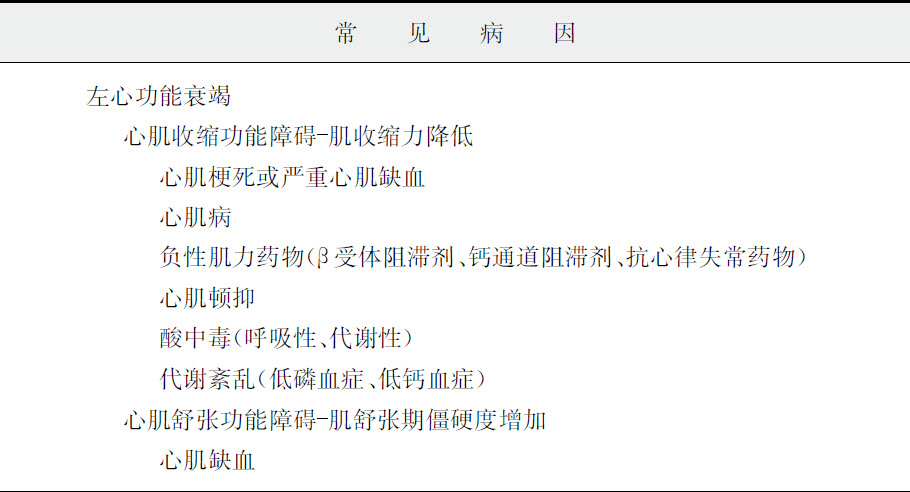
\includegraphics[width=5.95833in,height=4.26042in]{./images/Image00012.jpg}
\end{table}

近年来,机会致病菌性肺炎有增多的趋势。机会感染的致病条件为全身防御能力的严重降低,其诱因为:①基础疾病如恶性肿瘤,肝、肾衰竭,呼吸衰竭,糖尿病,大面积烧伤,白血病,器官移植后免疫抑制剂的应用,遗传性或获得性免疫缺陷综合征(AIDS)等;②附加因素如长期静脉(或膀胱)留置导管,气管插管,长期使用广谱抗菌药物致正常菌群失调,药物或放疗所致白细胞减少或反应性改变,以及T和(或)B淋巴细胞介导的免疫功能降低等。机会致病菌性肺炎有易感性、难治性和反复性等特点,临床症状多不典型,特别在糖皮质激素治疗中可无明显的发热和感染中毒症状。虽用抗生素积极治疗,但常迁延不愈,并发症多。目前革兰氏阴性杆菌已成为医院内机会致病菌性肺炎的重要病原,此外还有嗜肺军团杆菌、非典型分枝杆菌、肺孢子菌、巨细胞病毒、念珠菌、曲霉、隐球菌等致病微生物,经常威胁着患者的生命健康。

\subsection{3.1 感染性疾病}

\subsubsection{3.1.1 病毒性感染}

\paragraph{一、流感病毒性肺炎}

流感病毒性肺炎一般发生于流感流行高峰期间。患者除有流感本身的症状外,发病早期即有呼吸困难甚或发绀。肺部体征为叩诊轻浊音以及由两侧肺底向上蔓延的湿性啰音等。X线检查主要表现为间质性肺炎,并夹杂以不同形态的支气管肺炎样改变,可见肺内斑片状、多叶段渗出性病灶;进展迅速者,可发展为双肺弥漫的渗出性病变或实变,个别病例可见胸腔积液。季节性甲型流感(H1N1、H2N2和H3N2等)所致的病毒性肺炎主要发生于婴幼儿、老年人、慢性心肺疾病及免疫功能低下者,2009年甲型H1N1流感还可在青壮年、肥胖人群、有慢性基础疾病者和妊娠妇女等人群中引起严重的病毒性肺炎,部分发生难治性低氧血症。

流感病毒性肺炎的诊断根据是:①病例发生于流感流行期间,起病较急,在发病早期伴有显著的呼吸系统症状,如咽痛、流涕、咳嗽、呼吸困难,肺部可有啰音等;②血象白细胞数正常或减少;③X线检查肺部有肺炎征象,主要呈支气管肺炎和间质性肺炎表现,也可有肺实变表现;④曾用抗菌药物治疗而未见良效者;⑤鼻咽分泌物或口腔含漱液可分离出流感病毒或病毒抗原、核酸检测阳性。恢复期血清中抗流感病毒抗体滴度比急性期有4倍或以上升高有助于回顾性诊断。

流感病毒性肺炎主要须与肺炎支原体肺炎、肺结核等相区别。

\paragraph{二、高致病性人禽流感病毒性肺炎}

禽流感(禽流行性感冒)是禽类的甲型流感病毒亚型感染。1997年香港特别行政区出现人群暴发禽流感H5N1病毒感染,18例患者中6例死亡,是全球首次发现禽流感病毒能够直接感染人类。目前发现且证实可感染禽类又可感染人类的主要为禽甲型流感病毒H5N1、H9N2、H7N7和H7N9亚型,其中以H5N1亚型引起的病情重,病死率高。2013年3月底华东地区发现的H7N9禽流感病毒是全球首次发现的新亚型流感病毒,至2013年9月底我国内地共报告134例人感染H7N9禽流感确诊病例,其中死亡45人。人禽流感的传染源主要为患禽流感或携带禽流感病毒的鸡、鸭、鹅等家禽,特别是鸡;传播途径主要通过呼吸道,目前尚无人与人之间传播的确切证据。高危人群为与不明原因病死家禽或感染、疑似感染禽流感家禽密切接触人员。人禽流感的潜伏期一般为1~3天,通常在7天以内。临床上多为急性起病,早期表现流感样症状,主要为发热,体温大多持续在39℃以上,热程1~7天,一般为3~4天,可伴有流涕、鼻塞、咳嗽、咽痛、头痛和全身不适。部分患者可有恶心、腹痛、腹泻、稀水样便等消化道症状。重症患者病情发展迅速,可出现肺炎、急性呼吸窘迫综合征、肺出血、胸腔积液、全血细胞减少、肾衰竭、败血症、休克及雷氏(Reye)综合征等多种并发症。体检时重症患者有肺部实变体征。实验室检查外周血白细胞总数一般不高或降低,重症患者多有白细胞总数及淋巴细胞下降。重症患者胸部X线检查可显示单侧或双侧肺炎,少数可伴有胸腔积液等。其影像学特征有:①胸部X线主要表现为肺实质渗出性病变,两肺可见大片状及团絮状高密度影,中心区密度较高,边缘区密度较淡。阴影密度高于常见的病毒性肺炎;②影像学改变变化快,呈游走性;③典型病变病灶累及两肺,大致呈对称性,分布广泛;④临床症状与胸部X线表现不完全相符。病灶吸收落后于临床。诊断依靠流行病学史,结合临床表现和实验室检查,并排除流感、普通感冒、细菌性肺炎、严重急性呼吸综合征(SARS)、传染性单核细胞增多症、巨细胞病毒感染、衣原体肺炎、支原体肺炎等疾病后,可作出临床诊断。确诊有赖于病原学及血清学检测结果,最可靠的方法是从呼吸道标本中分离出禽流感病毒亚型。

\paragraph{三、严重急性呼吸综合征}

严重急性呼吸综合征(SARS)是新出现的传染病是由SARS冠状病毒所致的一种具有明显传染性、可累及多个脏器系统的特殊肺炎。主要通过飞沫、气溶胶或接触污染的物品传播。

潜伏期为2~10日,起病急骤,多以发热为首发症状,体温常>38℃,可有寒战、咳嗽、少痰,偶有血丝痰,心悸、气促,甚或呼吸窘迫。可伴有肌肉酸痛、头痛、关节痛、乏力和腹泻。患者多无上呼吸道卡他症状。肺部体征不明显,部分患者可闻及少许湿啰音,或有肺实变体征。抗菌药物治疗无效。患者的呼吸道症状和肺部体征与胸部X线检查的改变相比常常较轻。实验室检查外周血白细胞计数一般不升高或降低,淋巴细胞减少。胸部X线早期可无异常表现或淡薄阴影,随疾病发展可见不同程度片状、斑片状浸润阴影,或呈网状样改变;部分患者肺部病变进展迅速,呈大片浓密模糊炎性浸润阴影,边缘不清,分布在一个或数个肺叶(段),多为双侧改变,严重者呈“白肺”。肺部阴影吸收消散较慢,与临床体征可不一致。

诊断上强调流行病学史,疑似者可做血清SARS冠状病毒的特异抗体检测和鼻冲洗液或含漱液PCR检测,注意排除上感、流感、细菌性或真菌性肺炎、艾滋病合并肺部感染、军团菌病、肺结核、流行性出血热、肺部肿瘤、非感染性间质性疾病、肺水肿、肺不张、肺栓塞、肺嗜酸性粒细胞浸润症、肺血管炎等临床表现类似的呼吸系统疾病。

\paragraph{四、艾滋病}

艾滋病(AIDS)合并肺部病变引起发热并非少见。有作者提出有下列情况2项或以上者须考虑AIDS肺部病变:①双侧肺门周围网状或网结状阴影;②上述改变在3~5日迅速发展为两肺弥漫性肺间质肺实质浸润甚至为均质性肺实变;③结节样、线条样病变,伴有或不伴有肺门或纵隔淋巴结肿大;④肺部炎症经积极治疗无效甚至病灶发展增多。

如患者同时有下列1项危险因素伴1项相关症状时,即检测抗HIV抗体帮助诊断。

危险因素:①有静脉药瘾史;②有同性恋或异性乱交史;③10年内有输血或输血制品史;④来自流行地区曾与AIDS可疑患者接触史。

相关症状:①长期发热(>1个月)伴体重减轻;②慢性腹泻>1个月;③咳嗽1个月以上,伴气短;④剧烈头痛,甚至出现脑膜刺激征。

AIDS肺部感染的病原体主要有肺孢子菌,此外,巨细胞病毒、弓形虫、隐球菌、类圆线虫、军团菌、肺结核、非结核分枝杆菌等也可引起肺炎,请参阅有关章节。

\paragraph{五、巨细胞病毒肺炎}

巨细胞病毒(CMV)肺炎多发生在免疫抑制宿主,如恶性肿瘤、接受大量免疫抑制剂、细胞毒药物、放射治疗、AIDS等免疫功能低下者易罹患本病。近年器官移植病例增多,特别是肾移植、骨髓移植术后常发生严重的CMV感染,病死率高。如有以下情况,应高度怀疑巨细胞病毒肺炎:①免疫抑制宿主,器官移植受者多发生在术后2~4个月;②发热,体温多在38℃以上;③阵发性干咳,常伴有明显的呼吸困难;④多有全身症状,关节肌肉疼痛、腹胀、直立性低血压等;⑤肺部体征无明显异常;⑥X线胸片早期可能无异常发现,随病情发展逐渐出现双侧弥漫性间质性肺炎或肺泡浸润,肺外周和肺底部常被累及。

确诊需借助实验室检查,常用的检查包括病毒分离、PCR、核酸杂交、抗原血症、DNA血症、mRNA血症等。

\paragraph{六、腮腺炎病毒性肺炎}

国内报告一组成年人流行性腮腺炎并发肺炎的主要表现是临床症状与体征均不显著,仅少数有微热、咳痰或全身不适等症状。胸部X线检查发现肺野内散布有点状、小斑片状或大片状不均匀密度的阴影,通常以右下肺野较为显著,持续时间较长,为48~165天(平均95.7天)。血象无特殊改变。冷凝集试验阴性。磺胺类药物、青霉素、氯霉素治疗均不能使肺部X线征改善。肺部病变大概由于腮腺炎病毒侵犯肺间质及肺泡壁所致。

\paragraph{七、肺炎型传染性单核细胞增多症}

临床症状以发冷、发热、疲乏、淋巴结肿大、咽充血、肌酸痛、头痛、纳差等最为常见。肺炎的表现主要为咳嗽、胸痛,部分病例有血丝痰或铁锈色痰。体检仅1/3病例有肺实变征,但X线检查所有病例均有显著改变。X线胸片所见可分为斑片状、磨玻璃状、堆云状肺部阴影或肺纹理增多,其中以磨玻璃状阴影最具特征性。斑片状阴影与肺炎支原体肺炎所见者相似。病例都有传染性单核细胞增多症的血象,均呈阳性嗜异性凝集反应,经豚鼠肾吸收后,效价在1∶64~1∶2048之间。

此病主要须与肺炎支原体肺炎相区别,二者的X线征可有相似之处,且均可有阳性的嗜异性凝集反应与冷凝集反应,偶尔在传染性单核细胞增多症时,冷凝集试验效价可相当高,故阳性嗜异性凝集反应须经豚鼠肾吸附试验证实或(及)作冷凝集素类型测定,方有鉴别诊断意义。

此外,传染性单核细胞增多症时,血象多有大量的异形淋巴细胞出现,而在肺炎支原体肺炎则无此现象;前者对四环素类抗生素治疗的疗效不确定,也与肺炎支原体肺炎有所不同。表\ref{tab2-9}可作为二者鉴别的参考。
%\begin{table}[htbp]
%\centering
%\caption{肺炎型传染性单核细胞增多症与肺炎支原体肺炎的鉴别}
%\label{tab2-9}
%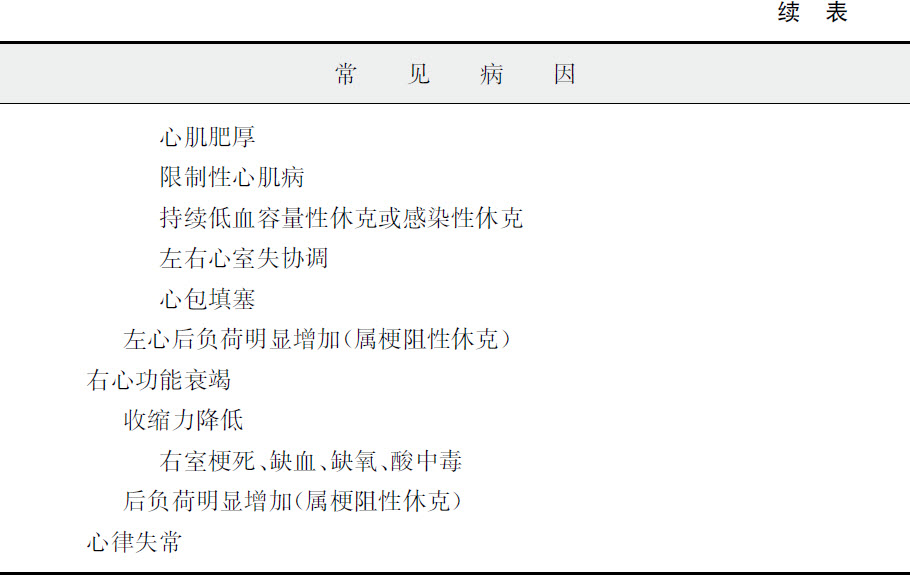
\includegraphics[width=5.96875in,height=2.25in]{./images/Image00013.jpg}
%\end{table}
%续表
%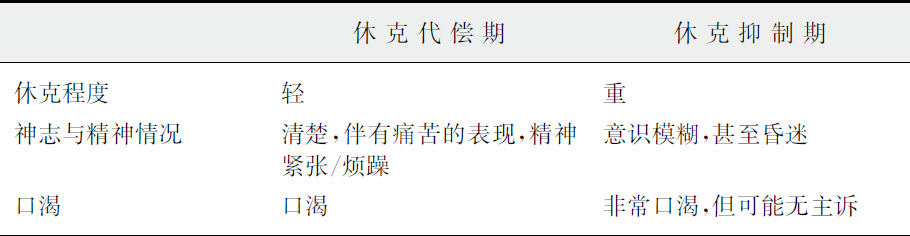
\includegraphics[width=5.90625in,height=1.33333in]{./images/Image00014.jpg}

\begin{longtable}{c}
  \caption{肺炎型传染性单核细胞增多症与肺炎支原体肺炎的鉴别}
  \label{tab2-9}
  \endfirsthead
  \caption[]{肺炎型传染性单核细胞增多症与肺炎支原体肺炎的鉴别}
  \endhead
  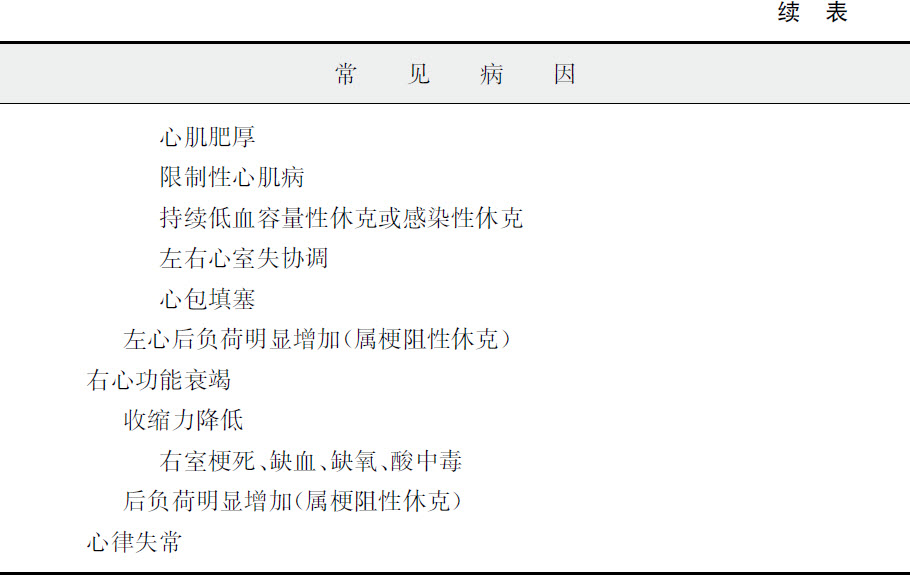
\includegraphics[width=\textwidth,height=\textheight,keepaspectratio]{./images/Image00013.jpg} \\
  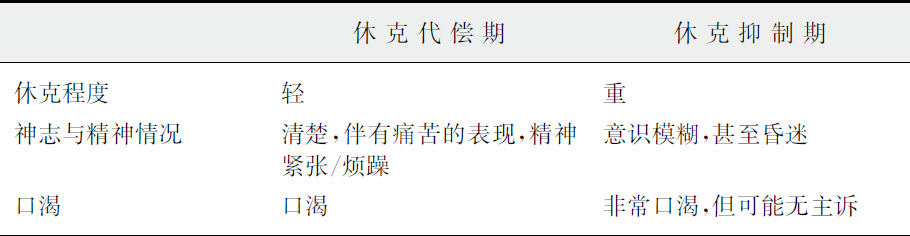
\includegraphics[width=\textwidth,height=\textheight,keepaspectratio]{./images/Image00014.jpg} \\
\end{longtable}

\subsubsection{3.1.2 细菌性感染}

细菌性肺炎的病原体因患病环境不同而有差异。社区获得性肺炎以肺炎链球菌、流感嗜血杆菌、卡他莫拉菌以及非典型病原体常见。医院获得性肺炎除了以上细菌外,还有金黄色葡萄球菌、铜绿假单胞菌、肠杆菌属和肺炎克雷伯杆菌等。病原体可通过空气吸入、血流播散、邻近感染部位蔓延、上呼吸道定植菌误吸、胃肠道反流物误吸和通过人工气道吸入环境中的致病菌引起。细菌性肺炎常以恶寒或寒战、高热起病,呼吸道症状较重,血白细胞增多常在15.0×
10\textsuperscript{9}
/L以上(肺结核可例外),分类以中性粒细胞占优势,并有明显的核左移与中毒性颗粒。血C-反应蛋白和降钙素原升高。

\paragraph{一、肺炎链球菌肺炎}

发病多见于冬春季节,青壮年男性罹患较多。发病前常有受凉、淋雨、饥饿、疲劳、醉酒病毒感染史。起病急骤,多以寒战突然起病,继而高热,多呈稽留热型。颜面潮红,呼吸浅速,甚至出现呼吸困难与发绀。患侧胸痛常见。咳嗽频繁,初为干咳,2~3天后咳出少量黏稠痰液,常呈铁锈色,以后逐渐变为脓性。可有唇疱疹出现。肺部病变部位常可发现轻浊音与捻发音。血象早期呈现白细胞增多、显著核左移与中毒性颗粒。

在病期第3~4天病变侵及整个肺叶,出现明显肺实变体征,浊音界与受累肺叶的境界相一致,听诊发现支气管呼吸音、细湿啰音与捻发音,此时临床诊断更为明确。

肺炎链球菌肺炎早期无特征性表现,凡患者突然畏寒或寒战、高热、胸痛伴肺部呼吸音减弱,白细胞增多,须考虑此病的可能性。胸部X线检查对早期诊断最有帮助。在发病后24~36小时作X线检查,受累肺叶可见有阴影出现,而此时体检可尚无典型的实变体征。此阴影通常从肺门向外周扩展,最后侵及整个肺叶,但目前典型的大叶性病变不多见。痰液涂片染色镜检及培养可证明肺炎链球菌的存在。尿肺炎链球菌抗原可阳性。

近年国内报道的重症肺炎,患者以中、老年人较多,但青壮年者也不少。患者的主要临床表现为高热或体温不升,呼吸困难,明显发绀,白细胞增多或减少,但核左移显著。重症肺炎有时局部体征不明显,甚至有时须经尸检才能证实诊断。

有的病例早期出现意识不清、谵妄、抽搐、昏迷、脑膜刺激征等症状,而肺炎体征尚未显露,易误诊为败血症、流脑、脑炎等疾病。个别病例表现为发热、腹痛、黄疸,可误诊为急性胆囊炎。个别右下叶肺炎患者呈右下腹痛,可误诊为急性阑尾炎。因此凡在肺炎多发的冬春季节,遇见原因未明的急性发热兼有上述表现者,切勿忽略肺炎的可能性,如病情许可应及时做X线检查以明确诊断。

\paragraph{二、肺炎克雷伯杆菌肺炎}

临床特点类似肺炎链球菌肺炎。国内报道的一组病例中,患者都为中年与老年男性,多发于慢性消耗性疾病与免疫力低下的基础上,如原有肺部疾病、糖尿病、手术后和酒精中毒的患者。此病发病急骤,以寒战、高热起病,并有胸痛、呼吸困难与发绀,患者呈急性重病容。神经精神症状也常见。重症病例可迅速发生休克而危及生命。痰为砖红色、血样,或胶冻样类似杨梅果酱,甚黏稠,但也可呈铁锈色。痰中可发现大量肺炎克雷伯杆菌。血象常呈中等度白细胞增多,核左移。肺实变体征可能早期出现,但无典型体征者较常见,甚至X线照片上显示大片致密阴影时,体检仅发现轻浊音和不明显的支气管呼吸音。主要并发症有脓胸、气胸、败血症和慢性肺炎等。

X线检查病变包括大叶实变、小叶浸润和蜂窝状脓肿(坏死性肺炎)形成。大叶实变多位于右上叶,重而黏稠的炎性渗出物使叶间裂呈弧形下坠。免疫功能抑制和慢性肺部疾患者表现为小叶浸润。16\%~50\%伴脓肿形成,形成单个或多个薄壁脓肿,最后遗留广泛性纤维性变或变为迁延性慢性肺脓肿。

临床上遇见年纪较大、全身情况较差的急性肺炎患者,痰中发现较多的疑似肺炎克雷伯杆菌时,应提高警惕。特别是在青霉素治疗下未见好转,肺部病变反而进展时,或在病程中迅速发生休克时,应立即作痰涂片及培养检查。

\paragraph{三、金黄色葡萄球菌性肺炎}

金黄色葡萄球菌引起的急性化脓性炎症。常发生于有基础疾病如糖尿病、血液病、艾滋病、肝病或原有支气管肺疾病者。儿童患流感或麻疹时亦易罹患。年老、体弱、较长期应用广谱抗生素或糖皮质激素等均为发病诱因。

多急骤起病,高热、寒战,发热多呈不规则型或弛张型,胸痛,痰脓性,可早期出现循环衰竭。此病与肺炎链球菌肺炎在临床上的不同点是:败血性经过,热程较长(2~4周),治疗显效后徐缓解热。特征性痰呈脓血性或黏液脓性,与肺炎链球菌肺炎的铁锈色痰有所不同。约半数病例出现皮疹,可为荨麻疹、出血性斑丘疹、瘀斑或瘀点等,而无唇疱疹出现。胸部体征早期不显著,仅呈轻浊音、呼吸音减弱及细湿啰音。胸部体征往往与严重的呼吸困难、发绀、血性痰、休克等症状不相称。

血白细胞增高,中性粒细胞比例增加,核左移并有中毒颗粒。此病的X线特点是:多发性小叶性炎症浸润阴影,但也可为大叶性,病灶内空洞形成、蜂窝状改变或肺气囊肿的出现等,其中尤以后者对诊断更有价值。痰、胸腔积液或血培养的阳性结果,有助于本病的确诊。

临床上如患者有下列表现之一时,须考虑金黄色葡萄球菌性肺炎的可能性:①恶寒或寒战、发热,咳嗽,胸痛,气促,咳脓血痰及伴有皮疹者;②败血症或流感后出现与胸部体征不相称的呼吸困难、发绀等症状,发热迁延不退或退热后又复燃者;③短期内两肺多发性炎症病灶,或一侧肺炎早期即出现肺脓肿、胸膜炎或肺气囊肿者;④已诊断为肺炎,但对青霉素治疗无良好反应者。遇此情况应做细菌学检查,同时加强抗菌药物的应用。

\paragraph{四、铜绿假单胞菌肺炎}

铜绿假单胞菌是医院获得性肺炎的常见病原体,它容易定植于呼吸道,广谱抗菌药物的使用会增加其定植风险。有文献报道4\%~15\%COPD患者痰中可分离到该菌。其近年来发病率呈上升趋势,且由于铜绿假单胞菌极易耐药,并不易为呼吸防御机制杀灭,治疗困难,病死率高。细菌的入侵途径通常是上呼吸道、皮肤与消化道。由于大面积皮肤烧伤合并铜绿假单胞菌感染而引起肺炎者也有时可见。高龄、体弱、原有慢性心、肺疾病、应用广谱抗生素以及器械污染等,是常见的发病诱因。

此病临床上除急性肺炎表现外,往往早期出现谵妄、发绀,并有倒错性发热(即热峰在每天上午出现)及相对缓脉。咳嗽时伴黄脓性痰,少数患者咳出的痰呈浅绿色。重症者可有低血压或休克。胸痛和咯血不常见。肺部X线征是双下肺广泛支气管炎性肺炎,伴有结节状阴影及多发性小脓肿形成,肺脓肿发生较早。

此病经过较重,预后凶险。血流感染发生率低,多见于免疫抑制宿主,因此确诊有赖于痰或胸腔积液的细菌培养。

\paragraph{五、支气管扩张并发感染}

支气管扩张并发急性细菌感染时,患者有发热、咳嗽、咳脓痰等症状,或咯血后出现感染的症状。X线胸片所见类似支气管肺炎、干酪样肺炎或浸润型肺结核。诊断须根据既往病史与治疗效果。如过去屡次在同一部位发生肺炎,则强烈支持支气管扩张合并感染的诊断。此病经积极的抗菌治疗后,往往迅速得到控制,大片阴影逐渐消失,成为索条状卷发阴影。有些感染经治不愈,要考虑是否合并非典型分枝杆菌感染、结核感染等。

\paragraph{六、急性肺脓肿}

急性肺脓肿根据感染途径可分成三个类型:

\subparagraph{(一)吸入性肺脓肿}

大多数肺脓肿主要由于吸入上呼吸道或口腔内带有细菌的分泌物所引起。全身衰弱、受凉、醉酒、中毒、鼻窦炎等常为发病基础。麻醉与手术、食物反流或呕吐、昏迷状态、溺水等均可为诱因,而睡眠中吸入感染则被认为是最常见的诱因。致病菌多为厌氧菌,其他常见菌有化脓性链球菌、金黄色葡萄球菌、肺炎克雷伯杆菌和铜绿假单胞菌等,但往往是多种细菌的混合感染。

患者往往以恶寒或寒战、高热、虚弱、胸痛、心率加快等症状急骤起病。体温常呈弛张热、稽留热或不规则型热。患者大多无呼吸困难与发绀。胸部体征常不显著,但也可呈轻浊音、呼吸音减弱或粗糙、散在性湿啰音等。白细胞显著增多与核左移。只根据胸部体格检查,易忽略肺脓肿的诊断,尤其是深在的肺脓肿往往无明显的体征。炎症浸润破溃后形成脓肿,脓肿向支气管穿破时患者突然咳出大量脓臭痰及坏死组织,静置后多可分为三层:上层为泡沫样痰,中层为黏液样成分,下层为坏死组织。

脓肿分布多位于右肺,右上肺的后段最常累及,其次为左、右下肺叶的背段。X线检查早期可见肺野有单个或多个界限模糊的片状阴影。嗣后此阴影的中心变为圆形透亮区,出现气液平面,转换体位时此气液平面随之改变,据此可以确定肺脓肿的诊断。

\subparagraph{(二)继发性肺脓肿}

某些细菌性肺炎(金黄色葡萄球菌、铜绿假单胞菌和肺炎克雷伯杆菌等)、支气管扩张、支气管囊肿、支气管肺癌、肺结核空洞等继发感染可导致继发性肺脓肿。支气管异物阻塞,也是导致肺脓肿特别是小儿肺脓肿的重要因素。肺部邻近器官的化脓性病变,如膈下脓肿、肾周脓肿、脊柱旁脓肿或食管穿孔等波及到肺也可引起肺脓肿。阿米巴肝脓肿好发于右肝顶部,易穿破膈肌至右肺下叶,形成阿米巴肺脓肿。

\subparagraph{(三)血源性肺脓肿}

通常并发于败血症,特别是金黄色葡萄球菌败血症的病程中。细菌性栓子血行播散到肺,引起小血管栓塞、炎症和坏死而形成肺脓肿。脓肿常为多发性,且常为双侧性。患者在全身感染的基础上发病,常伴高热、寒战、胸痛、咳嗽及血痰。痰量不多,肺部体征不明显。诊断主要依靠X线检查。胸部平片显示双肺多发性圆形病灶。脓肿形成后可见气液平面,有的形成张力性脓腔,可破裂而发生脓气胸。血培养常有致病菌生长,提示脓肿发生在败血症的基础上。也应细致检查其他器官的迁徙性化脓病灶。

\paragraph{七、肺结核}

血行播散型肺结核、浸润性肺结核、空洞性肺结核、干酪样肺炎、结核性胸膜炎等都可引起急性发热与肺部病征,临床上须与其他原因的肺部病变相区别。

\subparagraph{(一)血行播散型肺结核}

亦称急性粟粒型肺结核,多见于婴幼儿和青少年,特别是营养不良、患传染病和长期应用免疫抑制剂导致抵抗力明显下降的小儿,也可见于成人。起病急,持续高热,中毒症状严重。虽然病变侵及两肺,极少有呼吸困难,但也有发生急性呼吸窘迫综合征者。可有全身浅表淋巴结肿大,肝脾大,有时可发现皮肤淡红色粟粒疹和脑膜刺激征。体检时肺部叩诊与听诊体征轻微或缺如,与病情的严重性不相称,如不注意常易致误诊。X线胸片和胸部CT可见由肺尖至肺底呈大小、密度和分布三均匀的粟粒状结节阴影,结节直径2mm左右。参见第28节。

\subparagraph{(二)浸润性肺结核}

属于继发型肺结核,由新发的吸入感染,或由局限性病灶、播散性病灶恶化而成,为活动性肺结核。罹患者多在20~30岁。轻者无明显症状,有些患者呈急性发热,与流行性感冒的临床表现相似,其他为长期微热、心悸、盗汗、乏力、容易烦躁、微咳、咳痰、厌食、体重减轻等中毒症状。

肺部体征因病灶大小、数量及部位而定。病灶小者无异常体征。病灶较大或较多时,可出现轻浊音与细湿啰音(多在锁骨下窝部位)。血沉中等度增速。痰中常可检出结核杆菌。

X线检查显示下列特点:病变部位不定,在成年人多发生在肺尖、锁骨下部;病变多样性,阴影密度较浅,如絮状,边缘模糊,界限不清,可融合和形成空洞。

鉴别诊断上须与肺炎支原体肺炎、不完全性大叶性肺炎、肺吸虫病、支气管扩张合并感染等相区别。

下肺结核 下肺结核临床上少见,可见于艾滋病、糖尿病和其他免疫抑制患者的肺结核,病变位于肺门以下,发病右下叶多于左下叶。咯血是常有的症状;全身中毒症状与一般上肺结核无差异,但病程发展较快。发病常类似支气管肺炎。X线阴影特征与一般肺结核相同,但以大片状广泛浸润为多,且在早期即可有肺不张与空洞形成。早期诊断往往较为困难,最易误诊为肺脓肿与肺炎,有时甚至被误诊为肺包虫病。下列几点有助于早期鉴别诊断:

1.下肺结核患者有恶寒、寒战者少见。咳嗽与胸痛一般较肺炎或肺脓肿为轻,脓痰不多见,病程则较肺炎或肺脓肿为长。

2.大多数下肺结核患者的白细胞总数在正常范围内。

3.肺脓肿与下肺结核好发部位虽然都在肺下叶背段,但青年患者在下叶背段有空洞性病变,而症状与肺脓肿不尽相符时,应注意下肺结核的可能性。

4.下肺结核诊断的主要根据是痰中查得结核杆菌,应反复进行痰集菌涂片检查,必要时作培养或动物接种。

5.相当数量的下肺结核患者同时有支气管内膜结核,支气管镜检查是诊断的重要方法之一。

\subparagraph{(三)空洞性肺结核}

亦属于继发性型肺结核,临床症状较多,发热,咳嗽,咳痰和咯血等。空洞形态不一,可呈虫蚀样空洞、薄壁空洞、厚壁空洞、张力性空洞以及干酪溶解性空洞等,多有支气管播散病变。空洞内一般无气液平面,空洞周围炎性病变较少,常伴有条索、斑点及结节状病灶。痰中一般容易检到结核杆菌。合并肺炎时,应与肺脓肿相鉴别。

\subparagraph{(四)干酪样肺炎}

亦属于继发型肺结核,与浸润性肺结核不同,主要是干酪样变化比病灶周围炎变化显著,进展急剧,是严重的结核病类型。干酪样肺炎起于结核杆菌的支气管播散,在机体抵抗力极度降低和对结核杆菌过敏反应增高的情况下发病,临床与病理上可区分为大叶性干酪样肺炎与小叶性干酪样肺炎两种:

\hypertarget{text00025.htmlux5cux23CHP2-7-1-2-7-4-1}{}
1.大叶性干酪样肺炎

发病急,与肺炎链球菌肺炎相似,但温度上升较慢,经2~3天升至39~40℃,逐渐转为弛张热,并有恶寒、呼吸困难、胸痛、咳嗽、咳痰、痰中时有带血、纳差、极度疲乏等症状。体检可发现呈大叶分布的肺实变体征。X线检查发现大片阴影,数周后可溶解形成空洞,呈虫蚀样空洞。血象白细胞计数正常或轻度增多。大部分于发病一个月左右痰中发现结核杆菌。此病主要须与非结核性大叶性肺炎(主要是肺炎链球菌大叶性肺炎)相鉴别。干酪样肺炎发病较后者为慢,无唇疱疹,无铁锈色痰,颜面苍白而非潮红,痰中可找到结核杆菌,血中白细胞数通常在15.0×10\textsuperscript{9}
/L以下,对青霉素疗效不佳,且患者发病前往往已有食欲欠佳、消瘦、潮热、盗汗等结核全身中毒症状。由于此病经过严重,凡遇到大叶性肺炎而疑为结核性时,应即积极进行抗结核治疗,以免耽误病情。干酪样肺炎兼有空洞时须与肺脓肿相鉴别,前者有空洞形成时痰中应找到结核杆菌。

\hypertarget{text00025.htmlux5cux23CHP2-7-1-2-7-4-2}{}
2.小叶性干酪样肺炎

多见于病程长、治疗效果不佳、全身情况及抵抗力很差的慢性肺结核患者,或发生于并发糖尿病的肺结核患者,主要病变是散布于两肺的多数性干酪样病灶。这些病灶可同时或分批出现。X线胸片上显示大小不一、边缘模糊的阴影.可能为3~5片至7~8片不等。上述情况的患者如突然发生急性肺部感染的症状,如畏寒、发热、咳嗽、咳痰、脉快、呼吸困难、发绀等时,应考虑小叶性干酪样肺炎的可能性。体检可发现两肺散在性干性与湿性啰音,但叩诊浊音不显著。小叶性干酪样肺炎早期与非结核性小叶性肺炎不易鉴别,主要鉴别根据为前者血中常无白细胞增多,或仅轻度增多,而后者常有明显的白细胞增多;前者痰中常可找到结核杆菌而后者则无。

\paragraph{八、军团菌肺炎}

本病首次在美国(1976年)发现,近年国内多处亦发现有散发病例,还曾有暴发性流行。潜伏期2~10天。临床表现为倦怠、头痛、肌痛、发热(可达40℃或以上)和相对缓脉等,可有畏寒或寒战,或不同程度的消化道症状与精神神经症状。咳嗽逐渐出现并加剧,伴胸痛与咳黏液痰,痰数日后转为脓性。突出的血生化改变为低钠血症与低磷血症。部分病例可合并肝功能损害。典型X线胸片为早期一侧肺下野出现境界不清的浸润阴影,多呈斑点状间质浸润或致密性实变。其后扩大至一侧肺下野乃至一侧肺野。部分病例可累及双肺。1/3~2/3病例有不同程度的胸腔积液。患者痰液、胸腔积液和气管吸出物中均可检出军团菌。血清特异性免疫学检查亦有助于诊断。尿军团菌抗原及呼吸道分泌物直接荧光抗体染色法有助于本病早期诊断,前者敏感性是80\%~90\%,特异性是98\%~100\%,检测时间小于1小时,但后者敏感性较低。聚合酶链式反应(PCR)也有助于诊断,血、尿标本的敏感性为75\%~82\%,特异性90\%~100\%。诊断上本病与其他社区获得性肺炎相比较,头痛、腹泻、肌酸激酶值升高、严重低钠(<130mmol/L)、肝功能异常、对β-内酰胺类抗生素不敏感在军团菌肺炎中多见。1998年温思罗普大学发表了温思罗普大学医院(WUH)标准,以便于区分军团菌肺炎和其他细菌感染的肺炎(表\ref{tab2-10}\footnote{≥10分=临床诊断;5~9分=疑诊;<5分=排除。例1是临床诊断,例2为疑诊,例3排除})。但回顾性分析发现该标准能较好的区分军团菌肺炎和其他细菌感染的肺炎,但假阳性率较高。如用大环内酯类及氟喹诺酮类等药物治疗有效也支持诊断。另外,治疗后临床症状好转而胸片仍进一步恶化也是本病的特点之一。Fiumefreddo等提出另一社区获得性军团菌肺炎的临床诊断评分,分别是发热、无痰、血钠降低、LDH升高、C-反应蛋白升高和血小板降低6个指标,每项1分共6分,分值越高军团菌病可能性越大,≥4应高度怀疑军团菌病,此评分与WHU标准相比更为简单易用。其他还有CBPIS军团菌病评分系统也可应用(Clinical
Infectious Diseases.2003;37:483-9)。

\begin{table}[htbp]
\centering
\caption{WUH军团菌病评分系统}
\label{tab2-10}
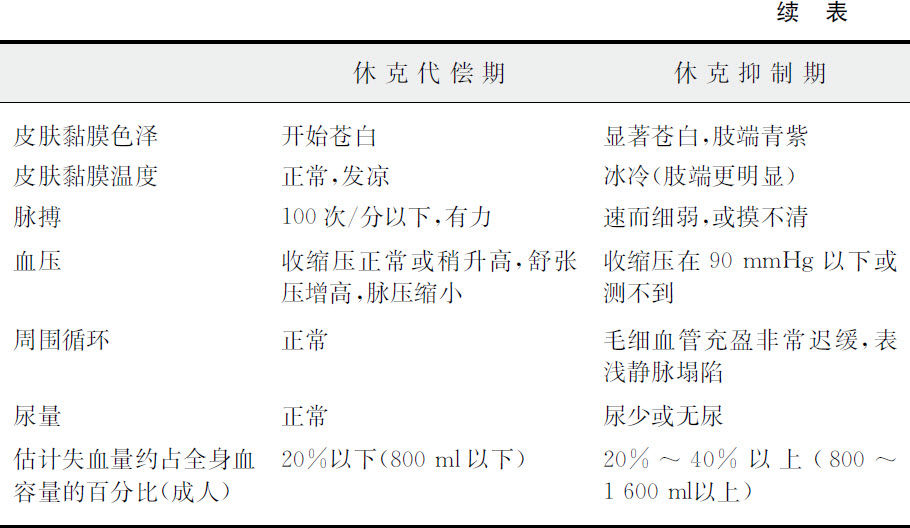
\includegraphics[width=6.03125in,height=6.58333in]{./images/Image00015.jpg}
\end{table}


据近年一组37例患者的综合分析,35\%有胃肠、肝、肾和神经精神异常的肺外症状,38\%有低钠血症,40\%合并胸腔积液,17\%合并肺脓肿。由此可见本病临床表现为全身性症状和呼吸系统症状。X线胸片肺部病变的恢复迟于临床改善,有些病例仍有进展。

\paragraph{九、肺型炭疽病}

诊断炭疽病须注意流行病学史。此病是重要职业病之一,主要见于从事畜牧、皮毛、毛织等职业的人,或曾与病畜接触的人。近年有用于生物恐怖活动。肺型炭疽病的发生是由于吸入混有炭疽杆菌芽胞的尘埃而致感染,又称“吸入性炭疽”,预后很差,但临床上少见。凡遇有急性发热患者伴有肺部感染症状,咳泡沫样血痰而兼有上述流行病学史者,须考虑有肺型炭疽病的可能性。

发病急骤,有寒战、高热、咳嗽、胸痛、大汗、心率增速、气促、喘鸣、发绀等症状,继而咳出锈色或血样痰。患者神志一般清醒。重症者发绀显著,血压下降,脉搏细速,有明显的休克现象。肺部体征仅可闻及散在的细湿啰音,或有胸腔积液征。体征与病情严重程度不成正比。血象白细胞数增高。

确诊须依靠细菌学检查。痰与胸腔渗出液直接涂片,均可发现革兰氏染色阳性、具有荚膜的粗大的炭疽杆菌。培养也容易获得阳性结果。

\hypertarget{text00025.htmlux5cux23CHP2-7-1-2-10}{}
十、肺型鼠疫

鼠疫是危害人类最严重的烈性传染病之一,病原体为鼠疫杆菌,传染源为受感染的鼠类或其他野生啮齿类动物。

鼠疫潜伏期多为2~3天,甚少超过5天。肺型鼠疫可分原发性与继发性两种。前者于发病后即出现肺部征象,表现为急性肺-胸膜炎;后者则继发于腺鼠疫之后。

肺型鼠疫发病急骤,患者有寒战、高热、胸痛、咳嗽、咳痰。痰最初为黏液性,后变稀薄稍带泡沫,不久可成为鲜红色血样,痰中含大量鼠疫杆菌。呼吸困难与发绀迅速出现。肺部体征多不明显,有时可发现肺部局限性浊音、散在性湿啰音与捻发音、胸膜摩擦音。X线检查可为正常或仅发现轻微病变,往往与病情的严重性不相称。肺型鼠疫常发展为败血症,未接受及时有效治疗者常于2~3日内死于心力衰竭、出血、休克,病死率高达70\%~100\%。

凡在鼠疫可能发生的地区和环境,遇有急性肺部感染患者,有明显的中毒症状、早期衰竭,或同时有淋巴结肿痛及出血现象,应考虑此病的可能性。痰液细菌学检查(包括涂片及培养)容易获得阳性结果,对确诊提供可靠依据。

\hypertarget{text00025.htmlux5cux23CHP2-7-1-2-11}{}
十一、类鼻疽肺病

类鼻疽是类鼻疽伯克霍尔德菌(类鼻疽假单胞菌)引起的人兽共患传染病,主要通过污染的水源、土壤经破损皮肤传染,或经污染的食物由消化道传染。其发病具有地域性分布,主要在热带和亚热带,属于地方性传染病,我国海南、广东、广西、福建、香港、台湾是多发地区。类鼻疽病多发于中年(22~66岁,平均47岁)男性,农民与渔民多见,大多有基础疾病,如糖尿病、继发型肺结核和类风湿关节炎等。畏寒、发热见于所有患者。急性肺部感染是类鼻疽病的最常见类型,约占70.5\%,可为轻症的肺炎至严重的坏死性肺炎。起病多急骤,恶寒或寒战、高热(多呈稽留热)、头痛、全身肌痛、胸痛、干咳或有咯血,呼吸困难、休克和败血症等,体检有局部皮肤脓肿、肝脾和淋巴结肿大,肺部体征少,可有湿啰音。大多患者血白细胞升高,中性粒细胞占优势。半数患者有肝功能损害,71\%血培养类鼻疽假单胞菌阳性。胸部X线大多数为肺上叶病变,有浸润病灶及(或)空洞,空洞多为单发,大小差异很大,少有液平,常可与肺炎、肺结核或其他慢性肉芽肿疾病混淆。确诊主要依靠病原菌分离及血清学检查。病原学标本可来自血液、脓肿液、痰液和尿液等,血清学检查则用标准类鼻疽伯克霍尔德菌诊断血清,类鼻疽特异性抗体可阳性。

\hypertarget{text00025.htmlux5cux23CHP2-7-1-2-12}{}
十二、肺型土拉菌病(兔热病)

土拉菌病一般发生在夏季,潜伏期通常为1周。起病急骤,体温迅速上升达39~40℃,伴全身乏力,畏寒,头痛,背痛,全身肌痛。病情发展时出现谵妄、昏睡、烦躁不安等急性全身中毒症状。患者体温升高持续2~5天,随之徐缓下降。细菌侵入部位的局部淋巴结首先有痛感,2天内皮肤呈现原发性病灶,多发于手或手指。开始呈红丘疹,继而发生脓疱,破溃后,形成中心性坏死,逐渐变成边缘较硬的溃疡。肿大的局部淋巴结,亦可破溃。病程一般持续3~4周,恢复缓慢,约需2~3个月或更长。伤寒型(全身型或胸膜肺型)的土拉菌病是一种小叶性肺炎,病程为迁延性(1~2个月或更长),有时痰中带血,有化脓的倾向。患者常有较轻的中毒症状,肺部体征不明显,无唇疱疹及显著的白细胞增多,但往往并发干性或渗出性胸膜炎。诊断依靠流行病学史及细菌血清学检查。

\subsubsection{3.1.3 衣原体感染}

衣原体是一种介于病毒、细菌和立克次体间的微生物,更近似于细菌,其大小约0.2~0.4μm。可引起肺炎的衣原体主要有肺炎衣原体(TWAR)和鹦鹉热衣原体两种,少数由沙眼衣原体引起。

\paragraph{一、肺炎衣原体肺炎}

肺炎衣原体可引起上呼吸道感染,如鼻窦炎、中耳炎和咽炎,也可引起下呼吸道感染,如支气管炎和肺炎。近年肺炎衣原体肺炎患病率有增高的趋势,多感染儿童和老年人,占社区获得性肺炎的6\%~19\%,国内近年报道一组665例社区获得性肺炎肺炎衣原体占6.6\%。起病多隐袭,早期表现为上呼吸道感染的症状,如声嘶、咽痛、发热等,症状通常较轻,数天或数周后患者上呼吸道症状减退,开始出现咳嗽,提示下呼吸道受累。其他症状有肌痛、头痛、不适和乏力。重症感染可有脓痰、呼吸困难等,多见于COPD和心力衰竭患者。可伴有肺外表现如中耳炎、结节性红斑、心内膜炎、关节炎、甲状腺炎、脑炎和吉兰-巴雷综合征等。X线胸片显示肺叶或肺段的浸润病灶,多见于下叶。

病原体分离培养、聚合酶链反应、血清学试验如微量免疫荧光(MIF)抗体试验和补体结合(CF)抗体试验等有助于确诊。本病需与病毒性肺炎、支原体肺炎、流行性感冒、肺结核、真菌感染等鉴别。

\paragraph{二、鹦鹉热衣原体肺炎}

鹦鹉热衣原体寄生于鹦鹉、鸽、鸡等100余种家禽和野生鸟类体内,主要感染禽类和低等哺乳类动物,人类并不常见。通常发生于与受感染鸟密切接触者,感染途径为通过呼吸道吸入疫鸟排泄物气溶胶所致。病原体吸入体内后首先进入肝脾的网状内皮细胞进行增殖,再经血路进入肺和其他器官,所以人类的鹦鹉热既可以是呼吸道感染,也可能是以呼吸道为主的全身感染。

起病多隐袭,病情轻者如流感样症状。重症肺炎者多有寒战、发热、体温逐渐升高,第1周内可达40℃以上,热程3~4周,伴乏力、头痛、关节肌肉疼痛,亦可有结膜炎、口腔炎、鼻出血或出现类似伤寒的玫瑰疹。1周左右才出现呼吸道症状,如咳嗽、少量咳痰或痰中带血,病变严重者可有呼吸困难及发绀。病程中尚可出现纳差、恶心、呕吐、腹痛、腹泻等消化道症状,心肌炎、心内膜炎及心包炎,亦可有嗜睡、谵妄、木僵、抽搐、意识不清等神经精神症状。体检肺部体征常较症状轻,病初可无明显体征,以后可有湿啰音,少数患者可有肺实变征或胸腔积液征。X线胸片显示早期从肺门向外放射的浸润病灶。病灶可融合呈叶性分布,以下叶多见。常有弥漫性支气管肺炎或间质性肺炎的X线表现。肺内病变吸收缓慢。

本病确诊须依靠衣原体分离培养及(或)特异性血清学检查。PCR诊断效果更佳。本病需与病毒性肺炎、支原体肺炎、流行性感冒、肺结核、真菌感染等鉴别。与肺炎衣原体肺炎的鉴别主要是后者通常无鸟类接触史,临床症状较轻,体温很少超过37.8℃,且很少累及呼吸道以外器官。微量免疫荧光(MIF)抗体试验可用于鉴别不同的衣原体。

\paragraph{三、沙眼衣原体肺炎}

沙眼衣原体包括15个血清型,引起人类沙眼、性病淋巴肉芽肿、包涵体性结膜炎、生殖道感染,以及新生儿肺炎。在极少数情况下,沙眼衣原体也引起免疫缺陷成人患者的呼吸道感染,甚至正常成人的社区获得性肺炎,病因不清。

沙眼衣原体新生儿肺炎主要见于2~12周新生儿及婴儿,通过感染的母亲产道时受感染。大多数无发热,起始症状通常是鼻炎、伴鼻腔黏液性分泌物和鼻塞。随后发展为断续的咳嗽,呼吸急促和肺部啰音,可伴有心肌炎和胸腔积液。肺部X线显示间质浸润。半数患儿可伴有急性包涵体性结膜炎。

\subsubsection{3.1.4 支原体感染}

支原体是介于细菌和病毒之间,能独立生存而不需要寄身于其他生物细胞的最小微生物,目前已知的支原体有80余种。

肺炎支原体肺炎

由肺炎支原体感染引起的肺炎称为肺炎支原体肺炎,此病秋冬季节多见,但季节性差异并不明显。青壮年较易罹患。国内调查占社区获得性肺炎的20.7\%,且多合并其他细菌感染。潜伏期1~2周,缓慢起病,发热呈中等度,多持续约1~2周,也可持续3周。咽痛与咳嗽是常见的症状,发病初期以阵发性干呛性咳嗽为主,以后约半数病例可咳少量黏液痰或痰中带血丝,或小量咯血,而无铁锈色痰。这种呛咳和痰的特征是大叶性肺炎所少见。全身症状较为明显,如乏力、头痛、咽痛、纳差、腹泻、肌痛、耳痛等。体格检查肺部体征与X线征不相称,虽X线检查有显著的改变,但肺部实变征象却不明显。

血象白细胞总数多数正常,分类可呈相对性淋巴细胞增多与轻度或中等度嗜酸性粒细胞增多,这与细菌性肺炎的鉴别有一定意义。血清冷凝集反应阳性率高达80\%,效价达1∶32或以上有诊断价值,于病程第2~3周阳性率较高。血清支原体IgM抗体≥1∶64,或恢复期抗体滴度有4倍升高,可进一步确诊。直接检测呼吸道标本中肺炎支原体抗原,可早期快速诊断。

X线检查肺部阴影往往在发病后2~5天出现,通常有下列三项特点:①肺纹理增多;②沿增多的肺纹理出现不规则的斑片状实质阴影;③多数改变集中于肺门附近。病变所在以下叶为多。上述的X线征大多于1~4周内消散。单纯依靠X线检查往往难于与不完全性大叶性肺炎、浸润型肺结核、癌性淋巴管炎等相区别。

肺炎支原体肺炎的诊断须综合全面检查结果而确定。主要根据是:①急性肺部感染具有感冒样症状,阵发性呛咳以及全身性症状;②X线检查有上述的改变;③血清冷凝集反应滴度在1∶32或以上,及(或)血清肺炎支原体IgM抗体滴度≥1∶64,或有4倍以上升高;④青霉素治疗无效而大环内酯类、氟喹诺酮类和四环素类抗生素有良好疗效;⑤有条件时可从痰或咽洗液中分离出肺炎支原体。近年有作者认为PCR技术可为肺炎支原体感染提供早期快速敏感特异的病原学诊断方法。

此病最易误诊,由于肺部实变征不明显,如无X线检查易误诊为流感或急性上呼吸道炎、支气管炎。有时患者因急性发热兼有上呼吸道炎症状,经常规X线胸部检查而发现。

\subsubsection{3.1.5 立克次体感染}

立克次体是介于细菌和病毒之间的微生物,有类似一般细菌的形态和结构,绝大多数又具有与病毒相似的在宿主细胞内才能生长、繁殖的特性。

\paragraph{一、Q热}

Q热是由Q热立克次体(贝纳柯克斯体)引起的急性传染病,大部分患者有间质性肺炎。许多野生动物、家畜、家禽都可自然感染。与病畜或其排泄物接触或饮用其生乳为主要的感染方式。

潜伏期9~26天,平均为10~14天,但在吸入感染时可缩短至3天。患者多以恶寒、高热而急骤发病。发热呈弛张热型,一般持续5~14天左右,然后迅速下降或于2~3天内降至正常。少数热程可持续3个月以上。剧烈的持续性头痛往往是此病的特征,肌痛与关节痛也常见。但与其他立克次体病不同,此病无皮疹,外斐试验阴性。

间质性肺炎通常在病期第3~4天出现。患者虽有肺部感染,但一般只有轻微的咳嗽,无痰或咳少量黏液性痰。胸部X线检查显示均匀模糊阴影,多侵及一个肺叶,尤以左下肺叶为多见。此病的特点是肺部体征多不明显或缺如,一般也无明显的呼吸道症状,但X线检查常能发现肺部有炎症。往往呈相对性缓脉,冷凝集试验阴性。

Q热的确诊须依靠病原体分离与血清免疫学检查。补体结合试验在病程第7~10天开始阳性(1∶32~1∶64),滴度逐渐上升,至第20~30天达高峰(1∶160~1∶640),以后逐渐下降。毛细管凝集试验的敏感性和特异性均较高。间接免疫荧光试验的抗体效价1∶64~1∶128或双份血清抗体效价升高4倍以上有诊断意义。

本病主要须与肺炎支原体肺炎相区别。肺炎支原体肺炎有较明显的上呼吸道症状,冷凝集试验常为阳性,但最可靠的鉴别方法仍为Q热立克次体分离或补体结合试验。

本病与布鲁菌病的传染源及传播途径有共同点,故二者混合感染亦有之。

\paragraph{二、恙虫病立克次体肺炎}

恙虫病的组织病理变化主要在血管系统,可见局灶性或广泛性血管炎、血管周围炎和血栓形成,导致全身多脏器损害,其中肺部损害较为常见,表现为肺充血、出血性肺炎或继发性支气管肺炎。

恙虫病临床特点为突然起病、高热、皮疹、淋巴结肿大、肝脾大和焦痂等。肺炎者主要表现为咳嗽,多为干咳或轻咳,可有咳少量白色黏痰、胸闷、胸痛,严重时可出现间质性肺炎,以呼吸困难为主,可出现发绀、急性呼吸衰竭。肺部体检可有湿啰音,少数有干啰音,或仅肺部呼吸音变粗。X线胸片提示肺浸润,双侧多见。肺间质炎症改变表现为肺纹理增多及模糊,呈网状影,并有小斑点病变。肺部炎性渗出病变表现为增粗肺纹理间可见斑片状、小片状、部分呈大片状密度均匀、边缘模糊阴影。可有肋膈角变钝与胸腔积液。合并急性肺损伤/急性呼吸窘迫综合征(ALI/ARDS)者胸部X线可表现双肺弥漫性浸润阴影、磨砂玻璃样改变。

恙虫病诊断上具备以下其中3项者可作诊断:①有野外接触史;②高热并发现特征性焦痂或溃疡;③淋巴结肿大、皮疹;④外斐试验1∶160以上。肺部合并症者除符合恙虫病诊断标准,有肺部临床表现和胸部X线改变外,需注意排除其他肺部疾患,如支原体肺炎、肺炎链球菌肺炎、浸润性肺结核等。

\subsubsection{3.1.6 螺旋体感染}

肺出血型钩端螺旋体病

肺出血型钩端螺旋体病即钩端螺旋体性出血性肺炎,是近年来比较多见的急性感染。患者多无黄疸,肝、肾损害较不显著,较易误诊。

据一组对43例患者资料总结的报道,大多起病急骤,有恶寒或寒战、高热、头痛、全身肌痛等症状,类似流行性感冒;部分起病较缓,仅轻微发热伴有鼻咽部症状,易与轻症流感或急性上呼吸道感染相混淆。2~3天后出现咳嗽、痰中带血、咯血、胸闷、气促及轻度发绀。有的病例发生大咯血,引起严重呼吸困难、发绀甚至窒息。患者肺炎症状虽显著,但胸部体征较少,仅部分病例叩诊呈轻度浊音和闻及湿啰音。患者通常并发心肌炎,表现为胸闷、脉搏加速与心电图改变。

X线征常在病程4~11天出现,也可较早或较迟,胸片上呈现双侧肺野斑片状模糊阴影,以中、下肺野尤著,其性质大多属于出血性炎症性实质性病变。胸部CT可见多形态变化表现,可早期发现X线胸片没有显示肺内出血改变,亦可显示病灶形态与分布范围,能判断肺部出血的程度。值得注意的是,部分病例在出血性肺炎症状尚未出现前已有异常的X线征,为早期诊断提供重要根据。

在有钩端螺旋体病的地区,值夏、秋季流行季节,遇有类似流感或急性上呼吸道感染患者,须警惕此病的可能性。患者发病前3~20天曾与疫水有接触史,尤其是初到该地区者,对提示诊断有重要意义。若患者已出现出血性肺炎症状,则可能性更大,但须与其他原因的肺炎、肺结核相鉴别。胸部X线检查对鉴别诊断帮助颇大,确诊须依靠病原学与血清学检查。

\subsubsection{3.1.7 真菌感染}

肺部真菌感染是最常见的深部真菌病。罹患者多有接受广谱抗生素、糖皮质激素、细胞毒药物或免疫抑制剂等治疗;或有慢性基础疾病如糖尿病,心、肺、肾、肝等疾病;或人免疫缺陷病毒(HIV)感染或艾滋病者。故诊断时应详细询问病史和用药史。从患者危险因素、临床特征、微生物学和组织病理学进行诊断分级,见表\ref{tab2-11}\footnote{\textsuperscript{a}
包括影像学;+:有,-:无;b肺组织、胸腔积液、血液真菌培养阳性;c除确诊标准外,也包括特异性真菌抗原检测阳性及合格的深部痰标本连续≥2次分离到同种真菌}。

\begin{table}[htbp]
\centering
\caption{侵袭性肺真菌病的分级诊断标准}
\label{tab2-11}
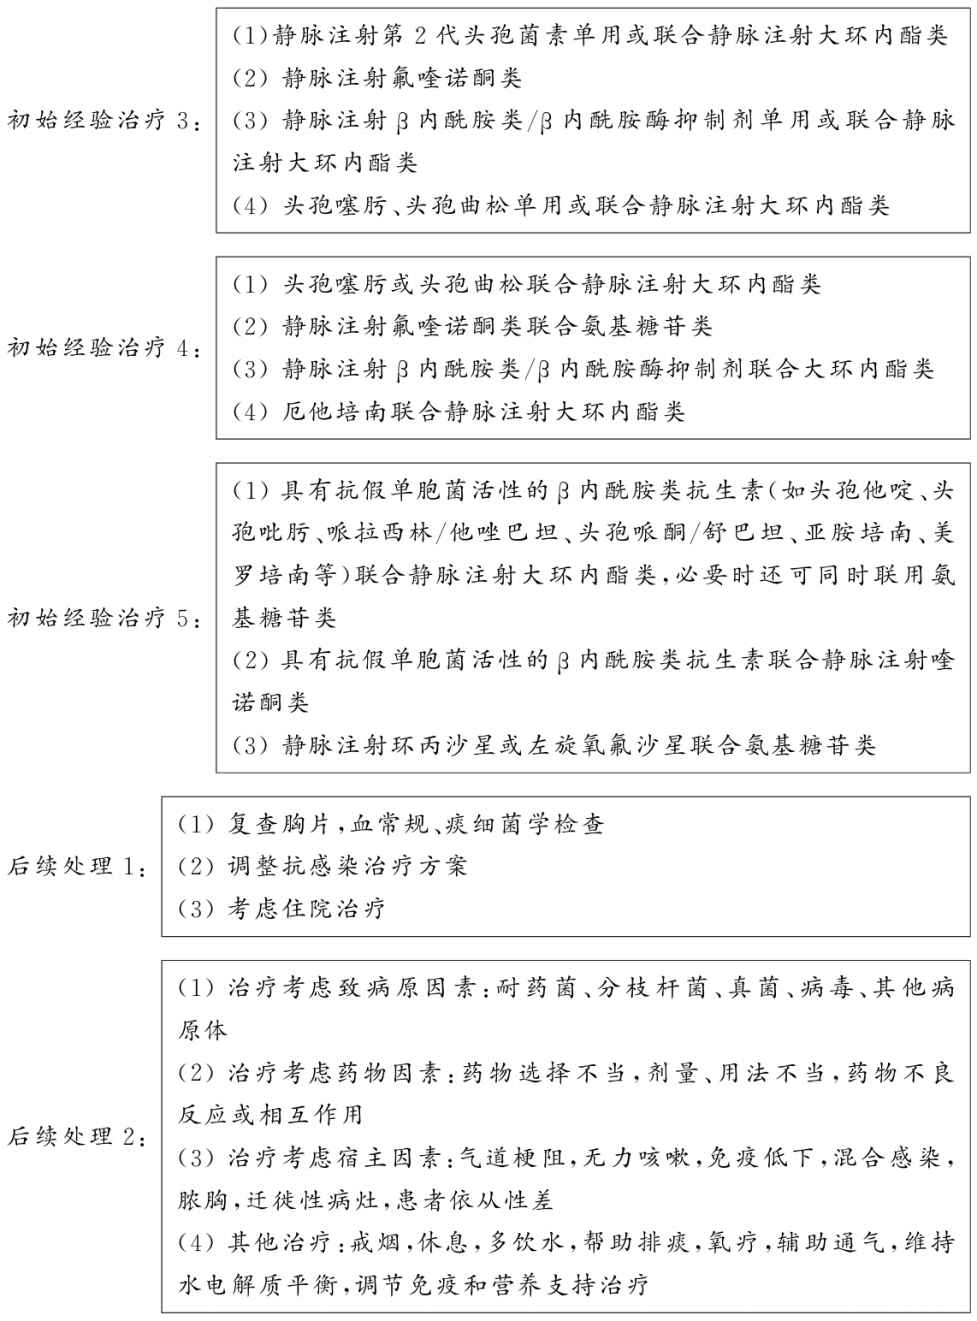
\includegraphics[width=5.94792in,height=1.08333in]{./images/Image00016.jpg}
\end{table}



\paragraph{一、肺念珠菌病}

有关肺念珠菌感染在临床上是多见还是很少见的问题一直存在争议。我国16家医院参加的肺真菌病调查显示该病仅次于肺曲霉病,位列第二。此病为白念珠菌或其他念珠菌所引起的急性、亚急性或慢性肺炎。感染途径主要是吸入,其次为血源性播散。临床上分为念珠菌支气管炎和念珠菌肺炎。支气管炎型表现为阵发性刺激性咳嗽,咳多量白泡沫塑料状稀痰,偶带血丝,随病情进展,痰稠如干糨糊状。憋喘、气短,尤以夜间为甚。乏力、盗汗,多不发热。X线仅示两肺中下野纹理增粗。肺炎型多发于免疫功能低下的患者,表现为畏寒、高热,咳白色泡沫黏痰,有酵臭味,或呈胶冻状,有时咯血,临床酷似急性细菌性肺炎。胸部X线显示双下肺纹理增多,纤维条索影伴散在的大小不等、形状不一的结节状阴影,呈支气管肺炎表现;或融合的均匀大片浸润,自肺门向周边扩展,可形成空洞。双肺或多肺叶病变,病灶时有变化,但肺尖较少受累。偶可并发渗出性胸膜炎。

诊断肺念珠菌病,要求合格的痰液或支气管分泌物标本2次显微镜检酵母假菌丝或菌丝阳性,以及真菌培养连续2次以上有同一菌种生长。另外,血清1,3-β-D-葡聚糖抗原检测连续2次阳性可做诊断参考。组织活检见有念珠菌菌丝侵入及炎症细胞浸润,可以确诊。

\paragraph{二、肺曲霉病}

肺曲霉病主要由烟曲霉引起,临床上主要有五种类型:侵袭性肺曲霉病、气管支气管曲霉病、慢性坏死性肺曲霉病、曲霉肿和变应性支气管肺曲霉病(ABPA)。这些类型的病变临床表现并不一样。

侵袭性肺曲霉病是最常见的类型,症状以干咳、胸痛常见,部分患者有咯血,病变广泛时出现气急和呼吸困难,甚至呼吸衰竭。部分患者可有中枢神经系统感染。中性粒细胞缺乏患者其X线胸片显示以胸膜为基底的多发的楔形阴影或空洞,病变早期胸部CT为晕轮征(halo
sign),后期为新月体征。但慢性阻塞性肺疾病合并侵袭性曲霉病时典型的CT改变很少见,而非特异性肺实变更多见。

气管支气管曲霉病病变主要在大气道,症状为发热、频繁咳嗽、少痰、胸痛、咯血。支气管镜检可确诊,可见气管支气管内假膜、溃疡、结节等病变。

慢性坏死性肺曲霉病亦称半侵袭性肺曲霉病,患者有长期呼吸道症状如咳嗽、咳痰等,也多有发热。X线显示慢性肺部空洞性病变。

曲霉肿(曲菌球)常继发于支气管囊肿、支气管扩张、肺脓肿和肺结核空洞。继发感染时可有发热,症状主要是刺激性咳嗽,常反复咯血,甚至大咯血,痰量一般不多。X线胸片显示在原有的慢性空洞内有一随体位改变而在空腔内移动的团球影。

ABPB为对曲霉过敏者吸入大量孢子后出现发热、喘息、畏寒、乏力、刺激性咳嗽、咳棕黄色脓痰,偶带血。患者多有哮喘病史。哮喘样发作为其突出的临床表现。X线胸片为上叶短暂性实变或不张,一过性肺浸润,磨玻璃阴影伴马赛克征。中央性支气管扩张(肺野内侧2/3的支气管)及壁增厚征象,有黏液嵌塞时表现为指套征或手套征。上述病变可发生于双侧。诊断标准见表\ref{tab2-12}。

\begin{table}[htbp]
\centering
\caption{ABPA诊断标准}
\label{tab2-12}
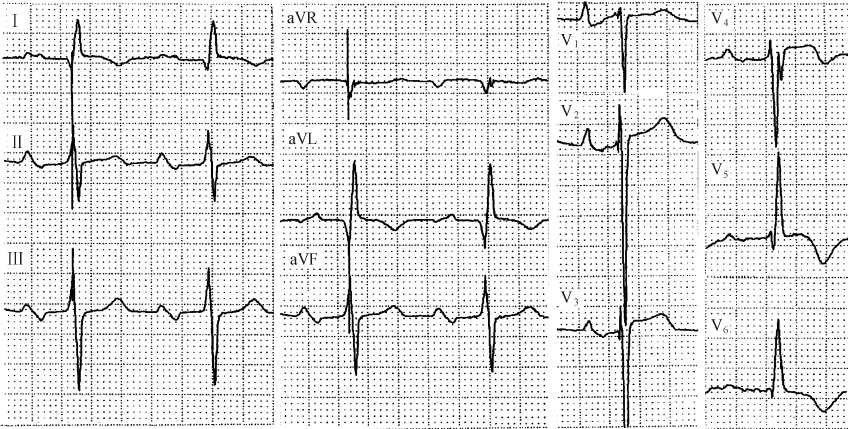
\includegraphics[width=5.97917in,height=1.84375in]{./images/Image00017.jpg}
\end{table}

诊断肺曲霉病除职业史(鸟禽饲养者、酿造工人、农业接触发霉稻谷者等)、机体免疫状态、临床表现及X线检查外,确诊有赖于组织培养及组织病理学检查,或呼吸道标本培养阳性,涂片见菌丝。血清曲霉抗体测定和血、尿、脑脊液及肺泡灌洗液曲霉半乳甘露聚糖测定和PCR测定血中曲霉DNA对本病诊断亦有帮助。变应性支气管肺曲霉病患者的诊断需与支气管哮喘相鉴别。

\paragraph{三、肺毛霉病}

肺毛霉病少见。此病常继发于糖尿病、肝硬化、结核病、恶性肿瘤、白血病及慢性感染的基础上,一般发生于终末期病变。病理改变主要为急性化脓性肺炎、多数性肺脓肿形成与肺坏疽。临床症状无特异性,主要为咳嗽、咳粉红色与黄红色痰、发热与白细胞增多。此霉可向全身播散,侵犯各脏器(心、肾、脑、肺等)。胸部影像学检查(尤其是胸部CT)可以显示单发或多发性浸润影或结节影,有时呈楔形改变,好发部位多为上叶,可双肺同时受累,下叶较少见。诊断有赖于组织病理学。

\paragraph{四、肺隐球菌病}

肺隐球菌病是由具有致病性的新生隐球菌及其变种感染引起的急性或亚急性肺真菌病,近年患病率有增加趋势。隐球菌经呼吸道侵入,在肺内形成感染灶,本病可呈急性、慢性或血源性播散,常引起隐球菌性脑膜炎。免疫抑制宿主(如AIDS)和健康人均可发病。临床分为无症状型、慢性型和急性型。急性型患者可有发热、咳嗽、咳黏液痰,盗汗、乏力和体重减轻。少数病例呈急性肺炎表现,高热、气急、低氧血症,可导致急性呼吸衰竭。以下线索诊断时可参考:①原先健康者肺部X线显示孤立或多发性结节状或块状阴影,特别是病变位于胸膜下时,常有空洞形成;毒性症状不明显;②免疫抑制患者出现肺部浸润,可单侧或双侧,可出现弥漫性间质性改变或粟粒状阴影;③肺部病变伴有脑膜炎表现者。

诊断可用痰涂片采用墨汁染色,可见圆形厚壁孢子,可有出芽现象,孢子内有反光颗粒,可提示诊断。组织活检可作最后诊断。播散型隐球菌病可做血、尿、脑脊液、皮肤损害的脓液等涂片及培养检查,阳性者可诊断。此外,乳胶凝集试验检测隐球菌荚膜多糖体抗原检测也有助诊断,非脑膜炎患者血清的阳性率为20\%~50\%。

\paragraph{五、肺孢子菌肺炎}

长期以来肺孢子菌一直被划归为原虫,但DNA研究证实肺孢子菌更接近于真菌,同源性介于子囊菌和担子菌之间。近年来核酸序列分析显示,人类与动物中分离出来的肺孢子菌差异很大。因此,国际上将从人类中检出的病原体改名为耶氏肺孢子菌(pneumocystis
jiroveci),而寄生于大鼠的则命名为卡氏肺孢子菌。同时建议保留PCP的缩写用法,但其含义改为肺孢子菌肺炎(pneumocystis
pneumonia)。肺孢子菌肺炎是免疫功能低下患者最常见以及最严重的机会感染性疾病之一。近年来发病率急剧增加,与免疫抑制剂、器官移植和艾滋病的流行有关。其感染途径主要为空气传染和体内潜伏状态肺孢子菌的激活。临床上分为流行型(经典型)与散发型(现代型)。流行型主要发生于2~6个月龄的早产儿、营养不良儿;散发型好发于免疫缺陷、肿瘤化疗、长期应用糖皮质激素或免疫抑制剂的儿童和成人。起病缓慢,早期有低热、腹泻、纳差、体重减轻,继而出现干咳、进行性呼吸困难、发绀等,常发生呼吸衰竭。体征常缺如,与症状的严重程度分离。胸部X线检查早期典型改变为双侧肺门周围弥漫性渗出,呈网状和小结节状影,然后迅速进展成双侧肺门的蝶状影,呈肺实变,可见支气管充气征。本病诊断有赖于活检组织特殊染色找到病原体。有文献报道实时定量PCR检测敏感性98\%,特异性96\%,可帮助分辨患者是否为PCP感染期。

艾滋病患者中PCP是最重要的机会感染之一,约85\%左右的晚期艾滋病患者合并PCP,25\%的艾滋病患者死于本病。近年国内报告的一组200例艾滋病患者中,已确诊PCP的有12例,其中4例合并结核病,1例合并肺炎链球菌肺炎。患者均有发热、咳嗽,干咳无痰;体温37.5~39.0℃,其中10例有呼吸急促、呼吸困难、发绀。肺部听诊2例有肺底部少许可变性湿啰音,2例少许干啰音。治疗前患者痰PCR检测均阳性,血PCR检测9例阳性;六胺银染色、吉姆萨染色找卡氏肺孢子菌分别有5例和6例阳性。

\subsubsection{3.1.8 寄生虫感染}

\paragraph{一、阿米巴肺脓肿}

阿米巴肺脓肿目前已比较少见。病变通常位于右下肺,因此病多由阿米巴肝脓肿穿破横膈至肺所引起,胸膜也同时累及。有时左叶肝脓肿向左膈穿破而引起左侧胸膜、肺阿米巴病。在少数病例中,阿米巴原虫由肠道病灶经血行传播至肺部,有些病例可无肝或肠阿米巴病病史,形成所谓“原发性肺阿米巴病”,易使人误会病变原发在肺。肺阿米巴病患者就诊时往往以发热、咳嗽、咳痰、右下胸痛与右肩放射痛为主诉,发热多为高热,弛张热型,伴或不伴寒战,可有气促、盗汗、纳差等症状。脓肿破入支气管时咳出大量酱红色或巧克力色黏稠脓性痰,对提示本病的诊断有重要意义。体检可发现肝脓肿体征。腹部B超和CT有助于诊断。

阿米巴肺脓肿的主要诊断依据是:①肠道或肝阿米巴病的病史;②大量典型的酱红色或巧克力色黏稠脓性痰,可检出溶组织阿米巴滋养体,但阳性率低于20\%;③右下肺叶病变,以及在X线透视下右膈局限性隆起与运动减弱等;④对甲硝唑(灭滴灵)治疗具有迅速而显著的疗效。疑似病例应考虑作抗阿米巴诊断性治疗。

\paragraph{二、急性血吸虫病的肺部病变}

急性血吸虫病较常并发肺部病变。肺部病变的出现距离感染期40余天至2个月左右,约2~3个月之后吸收并遗留少许痕迹。患者的临床表现有发热及其他毒血症症状等,伴有肝大压痛与外周血嗜酸性粒细胞增多。呼吸道症状大都轻微,咳嗽较常见,偶尔有咯血;胸部体征甚少,可有干、湿啰音。X线所见主要为弥漫性浸润,按其病灶显示的形态,可分为:①小斑片状阴影;②片状阴影;③大片状阴影;④粟粒状阴影等四类。

急性血吸虫病肺部病变的主要诊断根据是:①患者有急性血吸虫病的证据;②上述的肺部症状与X线征;③除外其他原因的肺部病变;④吡喹酮治疗疗效良好。

\paragraph{三、人比翼线虫病}

人比翼线虫病系罕见的疾病。自1913年发现以来,据报道全世界病例约100例。国内曾报道3例,一起进食未煮熟的鳖而致感染。主要症状为慢性阵发性咳嗽与咳黄痰,病程1个月后有血痰,体重减轻,亦可有胸痛。抗生素治疗无效是本病的特点。痰沉渣涂片检查可找到虫卵,孵化后虫壳内可见到幼虫。胸部X线表现无特殊性,大多数无异常发现,有的可表现为支气管炎或肺炎。纤维支气管镜检查所见主要表现为支气管黏膜充血,可有肉芽肿形成。特征表现是气管支气管内可见鲜红色血丝样的Y形线虫,钳出体外可见虫体蠕动。如怀疑此病可嘱患者仔细观察咳出的痰,有时可见虫体而诊断。

\protect\hypertarget{text00026.html}{}{}

\subsection{3.2 变态反应性疾病}

\subsubsection{一、单纯性肺嗜酸性粒细胞浸润症(吕弗勒综合征)}

单纯性肺嗜酸性粒细胞浸润症又称吕弗勒综合征(Löffler's
syndrome),主要特点是短暂而易消散的肺部浸润阴影,伴以短暂的外周血嗜酸性粒细胞增多。多数病例有短期的发热。参考第7.2.3节。

诊断本病的主要依据是:①病程短暂与良性经过;②发热、咳嗽、咳痰,肺部听诊可有干性或湿性啰音等症状与体征;③外周血嗜酸性粒细胞增多;④X线检查肺部有短暂性浸润阴影,呈游走性,消散后不留痕迹。

\subsubsection{二、风湿性肺炎}

风湿性肺炎少见,一般发生于风湿热的基础上。临床表现一般可区分为轻、重两型。轻型病例仅轻微咳嗽,偶有血丝痰,肺部可发现湿啰音,病变局限,可并发胸膜炎,预后较佳,因症状轻微,临床上易被忽视。重型病例病变广泛,往往突然出现脉快、心悸、气促、发绀、胸痛、咳血丝痰等症状,体温波动较大,病情较重,但肺部体征却轻微甚或缺如。X线表现多种多样,出现迅速,消散也快,有时呈游走性反复出现,连续X线检查,对临床诊断常起决定性作用。

风湿性肺炎的诊断主要根据:①有符合风湿热的临床表现;②上述的胸部症状与X线征;③除外其他原因的肺部病变,如过敏性肺炎、肺炎支原体肺炎等。抗链球菌溶血素“O”测定及C反应蛋白反应,对此病的诊断往往有帮助。

\protect\hypertarget{text00027.html}{}{}

\subsection{3.3 风湿性疾病}

许多风湿性疾病可有发热和肺部浸润。系统性红斑狼疮可有间质性或小叶性肺炎等肺部表现,常与胸膜炎并发。狼疮性肺炎表现为发热、干咳、气促,X线胸片可见片状浸润阴影,多见于双下肺。因多有白细胞减少,且抗生素治疗无效,可误诊为病毒性肺炎,但激素治疗后肺炎迅速消退。类风湿关节炎、系统性硬化病、多发性肌炎-皮肌炎等可有发热和肺部浸润病变,结节性多动脉炎的肺部病变多伴有咯血。临床上应注意鉴别,目前由于免疫学检查的普及,诊断一般不难。

\protect\hypertarget{text00028.html}{}{}

\subsection{3.4 化学性及物理性损害}

\subsubsection{一、化学性肺炎}

在化学工业生产过程中或其他原因而致吸入高度刺激性的化学性气体(如氮氧化物、硫化氢、氯、二氧化硫、汽油等),可引起急性肺部病变,表现为肺炎与急性肺水肿。

\paragraph{(一)汽油吸入性肺炎}

患者以汽车司机及其助手为多见,一般在吸入后立即发生剧烈咳嗽,并常有咯血,2~8小时后体温开始上升,大多数持续于38~39.5℃之间,最高达40℃以上。其他常见症状为胸痛、头痛、头晕、昏厥、恶心、呕吐、呼吸困难等。体检出现肺部浊音、肺泡呼吸音减弱、湿啰音等。X线检查在发病后3~6小时内,一般即可发现肺部大片密度不均匀,边缘模糊的实变阴影,后者与肺门相连,其周围有散在性、密度不甚高的斑点状阴影。此病如能及时恰当处理,一般预后良好。

\paragraph{(二)胃酸吸入性肺炎}

系胃酸反流吸入引起的化学性肺炎,亦称孟德尔森综合征(Mendelson
syndrome)。以年长者居多。临床上以胃酸反流后出现咳嗽、发热、呼吸困难为主要表现,继而出现急性呼吸窘迫综合征(ARDS)。本病国外报道较多,临床对发热、很快出现呼吸窘迫、发绀的患者,尤其是老年患者应注意鉴别。

\subsubsection{二、药物性肺病}

有些药物如呋喃妥因、青霉素、碘、复方乙酰水杨酸、异戊巴比妥等可引起变态反应性肺部病变,发病急,表现为发热、全身性皮疹、双肺湿啰音、X线胸片呈斑片状阴影等。诊断时需仔细寻找用药史。

\subsubsection{三、急性放射性肺炎}

急性放射性肺炎是由于放射线治疗胸部疾病(如支气管肺癌)所引起的一种合并症。此病发病较急,预后不良,目前尚无有效疗法。急性放射性肺炎的诊断主要根据下列各点:①病史:胸部曾接受大面积高剂量的放射治疗,发病前有感冒史;②症状:干咳、气促、微热,进行性病情加重;③体征:有发绀、呼吸困难,照射区内叩诊浊音,并可听到湿性与干性啰音;④化验检查:白细胞总数不增多;⑤肺部X线检查:照射野内有密度增高的片状或网状阴影,尤以肺门区为显著。

\protect\hypertarget{text00029.html}{}{}

\subsection{3.5 特发性间质性肺炎}

\subsubsection{一、急性间质性肺炎}

急性间质性肺炎(AIP)又称Hamman-Rich综合征,是一种病因未明、起病急骤、病情危重,以肺部弥漫性浸润并迅速发展为呼吸衰竭为特征的肺部疾病。患者起病突然、进展迅速,在较短时间内出现呼吸衰竭,平均存活时间很短,大部分在1~2个月死亡。绝大部分患者在起病初期有类似上呼吸道病毒感染的症状,半数以上的患者突然发热、干咳,伴进行性加重的呼吸困难。双肺底可闻及散在的细捻发音。实验室检查不具有特异性。X线胸片显示双肺广泛弥漫性浸润阴影。近年国内文献已有报道。本病临床表现为病情急剧进展的急性呼吸系统疾病,患者有发热、咳嗽、进行性呼吸困难乃至快速导致呼吸衰竭。X线胸片显示双肺广泛弥漫性浸润阴影。病因与发病机制尚未明了。诊断须排除各种已知原因的急性肺疾病方能确定,尤须与ARDS相鉴别,主要根据临床和病理的认真分析以及糖皮质激素的治疗效果。

\subsubsection{二、隐源性机化性肺炎}

隐源性机化性肺炎(COP),指不明原因的机化性肺炎(OP),是一种以细支气管、肺泡管、肺泡腔内肉芽组织栓形成为特征的肺部非特异性炎症过程,包括继发性机化性肺炎和隐源性机化性肺炎(COP)。后者指没有明确病因的“特发性”机化性肺炎。以往曾称为闭塞性细支气管炎伴机化性肺炎(BOOP)。该病主要表现为干咳、呼吸困难,呼吸困难多为活动后气短,程度多数较轻,部分患者可出现发热、纳差、体重下降。胸片可表现为双侧斑片状浸润影,主要分布于胸膜下及肺野外带,在病程中可有游走性。胸部CT表现分为:①多发性肺泡实变影(典型COP):多见于双肺胸膜下或沿支气管血管束分布,病变大小从几厘米到整个肺叶不等,可有支气管充气征及游走性表现。②浸润性阴影(浸润性COP):表现为双肺底网织状阴影伴磨玻璃影,浸润型由定义不清的弓形病变或小叶旁的多角形病变组成,通常伴随着其他阴影尤其是实变影。③局灶性实变影(局灶COP):局灶肺泡浸润影常位于上肺,边缘清楚,常呈叶、段分布,偶有空洞。肺部影像学具有多发性、多态性、易变性和病变多在肺外周的特点,加上抗生素治疗无效,临床诊断并不困难。糖皮质激素治疗效果一般较好。

\protect\hypertarget{text00030.html}{}{}

\section{4 周期性发热}

患者的体温突然或徐缓上升到高峰,保持数小时乃至若干天,然后迅速或徐缓下降至正常,经若干天无热期后又再发热,历数小时至若干天后又下降至正常。如此发热期与无热期互相交替,反复多次,即周期性发热。周期性发热原因可分为感染性与非感染性两类(表\ref{tab2-13})。

\begin{table}[htbp]
\centering
\caption{周期性发热的疾病分类}
\label{tab2-13}
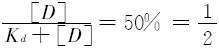
\includegraphics[width=5.92708in,height=2.9375in]{./images/Image00018.jpg}
\end{table}

\subsection{4.1 感染性周期性发热疾病}

\subsubsection{一、波状热(布鲁菌病)}

波状热的主要传染源是受感染的羊、牛与猪。文献报告约15\%~22\%病例具有典型的波状热型、每次发热期自6天至数周不等,一般有几个热波,可自行退热而进入缓解期,经数天至数周,热度又见回升。此种反复发生的周期性发热可迁延累月经年之久(参见第5.1节)。

\subsubsection{二、局灶性细菌性感染}

肾盂肾炎、支气管扩张合并感染、血栓性静脉炎、胆囊炎等部位处受到细菌性感染,都可引起反复的发热或寒战发作,但间歇期并无规则。

一侧慢性腰痛伴有原因未明的间歇性发热,除慢性复发性肾盂肾炎之外,肾结核也须考虑。国内报告不典型肾结核,可仅以间歇性发热为临床的唯一表现。

对于反复发生细菌性感染的患者,尤其是同类病原体引起的反复感染(如肺炎双球菌性肺炎),应考虑低(或无)丙种球蛋白血症或无能丙种球蛋白血症的可能。低(或无)丙种球蛋白血症可为先天性或获得性。诊断方法主要是测定血清中免疫球蛋白定量,缺乏IgG或7S丙种球蛋白时,抗细菌、抗病毒的抗体也常缺乏,致反复发生感染。无能丙种球蛋白血症与低丙种球蛋白血症不同,患者的血清蛋白电泳有高于正常或正常量的丙种球蛋白,只是表现丙种球蛋白的功能有缺陷,免疫功能低下,对各种感染有极大的易感性,人工自动免疫试验无抗体形成(如接种伤寒菌苗后,肥达反应阴性)。本症可为特发性或继发性,常继发于骨髓瘤、淋巴瘤、白血病等。

\subsubsection{三、败血症、亚急性感染性心内膜炎}

在败血症与亚急性细菌性心内膜炎病例中,有时可出现间歇性发热,类似疟疾发作,如不注意详细检查,可致误诊(参见第1.1节)。

\subsubsection{四、回归热}

回归热是由回归热螺旋体引起的急性虫媒传染病,引起人类发病者有虱传和蜱传回归热螺旋体,前者国内已罕见报道,后者散发于世界各地,我国以南疆及山西等地为主要发病地。本病特点为急起急退的高热,短期热退呈无热间歇,数日后又反复发作,发热期与间歇期交替反复出现,并有全身肌肉酸痛、肝脾大。间歇期除感虚弱外,其他症状均减退或消失,血白细胞多增高,也可正常,中性粒细胞增多。发作次数频繁者贫血严重,可有丙氨酸转氨酶升高,凝血酶原时间延长等,发热期采血涂片检出螺旋体可确诊。

回归热可分为流行性回归热与地方性回归热二型。前者以体虱为传染媒介,症状较重;后者由壁虱传播,症状较轻。

在流行性回归热多发的冬春季节及地区,如患者有寒战、高热、头痛、肌痛、鼻出血,并发现带虱或曾与此病患者有密切接触史者,须考虑此病的可能性,应作厚滴血片或血涂片镜检回归热螺旋体。

据国内报告;地方性回归热发病季节以4~8月为高,有严格的地区性,诊断地方性回归热须注意以下几点;①发病急骤.发热呈不规则的间歇型,初次发作持续时间为2~6天。以后发作仅持续数小时至一天。无热期长短不一,自1~14天,因而呈现不规则的周期性发热曲线。②症状较流行性回归热为轻。③患者无带虱现象,反之往往有被壁虱刺咬史。④血液及骨髓涂片中螺旋体数量虽稀少难找,但在无热期也可找到;动物接种易于成功。⑤青霉素治疗无效,胂剂一次疗法大都复发。

有报道:女,17岁,新疆人,周期性发热3个月,每周发热1~3次,午后发热,体温达40℃,中度贫血,血涂片检出回归热螺旋体,青霉素治疗14天,未再发热。

回归热须与钩端螺旋体病、流感、斑疹伤寒、疟疾、波状热等相区别。可依靠流行病学史、临床动态观察、病原学与血清学检查,一般困难不大。

\subsubsection{五、鼠咬热}

鼠咬热罕见。引起鼠咬热的病原体已证实有两种:一为小螺旋体,一为念珠状链杆菌。国内报告的病例大都由前者引起。由后者引起的仅属个别病例。

诊断鼠咬热首先须注意鼠咬史。由小螺旋体引起的鼠咬热有以下临床特征:潜伏期5~21天。患者通常以寒战、高热急骤发病,全身症状较重。最有诊断价值的特征是在鼠咬部位发生热、肿、痛,呈紫黑色,可形成水疱、组织坏死或硬性下疳样溃疡,上覆以黑色痂皮,并有局部淋巴结炎。发热持续数天而骤退,但经数天后又再发,呈回归热型、发热期间鼠咬伤部位炎症加剧,患者可发生皮疹,抽血作暗视野荧光检查,可发现活动迅速的小螺旋体,在皮肤损害处采取分泌物或肿胀的局部淋巴结穿刺检查,更易获得阳性结果。胂剂或青霉素治疗有效。

由念珠状链杆菌引起的鼠咬热,症状基本与上述相似,但潜伏期较短,仅1~5天,咬伤处炎症反应不显著,胂剂疗法不理想,但青霉素治疗有良效。可将患者血液作培养或接种于小白鼠腹腔内而确定诊断。

鼠咬热须与疟疾、回归热、斑疹伤寒及败血症等相鉴别,主要根据鼠咬史与病原学检查。

\subsubsection{六、间日疟}

凡在夏、秋季节,患者有周期性发冷、发热、盛汗,呈隔日发作兼有脾大与贫血,须考虑间日疟的可能性。如患者在疟区居留或最近曾到过疟区,间日疟的临床诊断大致可以成立。血涂片发现间日疟原虫是确诊的可靠依据。

在各种疟疾中,间日疟较为多见。分布也较广。潜伏期通常为10~14天,输血疟疾则较短(7~10天)。

患者以突然寒战急骤发病,颜面苍白,虽盖厚被仍未能止冷。发冷持续约1/2~2小时,继而体温迅速上升,高热往往达40~41℃。此时患者颜面转为潮红、头痛、口渴,有时谵妄;皮肤干热,脉快。发病5~7小时后开始大量出汗,持续约2~3小时衣摆尽湿,体温恢复正常或降至常温以下。整个发作过程持续6~10小时,单纯感染者每隔48小时周期发作一次。发作多在中午至下午,经数次发作后,脾脏可触及,并出现继发性贫血。有的病例出现唇疱疹,对诊断有一定意义,因唇疱疹少见于其他类型疟疾。

典型间日疟的临床诊断较易,但二重感染者、混合感染者(常见是间日疟合并恶性疟)以及曾接受不规则抗疟治疗者症状常不典型,易误诊为其他急性发热疾病。此时作厚滴血片或血涂片镜检疟原虫是确定诊断的最简捷方法。如厚滴血片阴性,必要时可作骨髓穿刺涂片检查。口服氯喹作诊断性治疗可用于高度疑似的病例。

\subsubsection{七、三日疟}

三日疟比较少见,大多为散发性。病初发热不高,呈不规则型、弛张型热,3~5天后较为典型发作,症状与间日疟相似。有发冷、发热及出汗阶段,但每隔72小时发作一次,且多在午后发作。单纯感染者发作周期经常不变。发作数次后出现脾大与贫血。

三日疟的临床诊断可根据典型的周期性发作、脾大与继发性贫血。二重感染者可每发作二天间歇一天,三重感染者可每天发作,因而必须注意与其他发热性疾病相鉴别。血涂片镜检发现三日疟原虫是诊断的最可靠依据。

\subsubsection{八、蛋形疟}

蛋形疟是最少见的疟疾,流行季节为4~7月和10~12月。蛋形疟的发作周期与间日疟同,也为48小时,但其发作常在黄昏或晚间。临床症状轻重不一,轻症者可无明显症状,重症者发热可达41℃或以上,并可持续十余小时之久,甚至发生谵语。此病在治愈后不易复发。确诊须依靠从血液中检出蛋形疟原虫。

\subsubsection{九、黑热病}

有些黑热病患者的早期症状与波状热相似,体温曲线呈波状起伏,并有大量出汗,脾大与白细胞减少。这种情况甚至使人不会想到黑热病。偶尔早期患者的血清可凝集布鲁菌,但滴度不超过1∶160。另一方面,有时早期黑热病的症状可酷似间日疟,但血片镜检疟原虫始终阴性,抗疟治疗无效。

黑热病的诊断须根据流行病学史、临床表现与骨髓穿刺检查。

\subsubsection{十、丝虫病}

丝虫病患者发作丝虫热时,通常在剧烈运动或疲劳之后,突以畏寒或寒战而起病。继而体温急骤上升,可达40℃,伴淋巴管(结)炎,持续1~3天而消退,但也可持续达一周之久。往往每隔2~4周或数月发作一次。

\subsubsection{十一、战壕热(五日热)}

战壕热可以每隔五天出现寒热发作为特征,并有皮疹,腰、腿肌痛与胫骨痛,病程长短不一。此病是一种立克次体感染,传染媒介为体虱,国内未发现。

\subsubsection{十二、其 他}

偶见有钩虫病致周期性发热3个月,间歇3~4天发热1次,持续3~4小时自退,患者有嗜酸细胞增多,贫血,大便隐血弱阳性,粪找虫卵阴性。胃镜发现十二指肠降部数条钩虫。

\protect\hypertarget{text00031.html}{}{}

\subsection{4.2 非感染性周期性发热疾病}

\subsubsection{一、结节性脂膜炎}

结节性脂膜炎(Weber-Christian病)是一种原发于脂肪小叶的非化脓性炎症,是较少见的一种变态反应性疾病。好发于青壮年女性。根据受累部位,可分为皮肤型和系统型。

临床表现以反复全身不适、关节痛、发热、皮下结节为特征,受累的皮肤反复发生红斑,时有压痛,并有水肿性皮下结节,损害呈多发性、对称性、成群分布、最常受累的部位是双下肢,常伴全身不适,发热与关节疼痛,亦可出现恶心、呕吐、腹痛、体重下降、肝脾大及其他内脏损害,其病程有很大差异,主要取决于受累器官的情况,内脏受累广泛者,可出现多脏器功能衰竭、大出血或并发感染。

结节性脂膜炎发热的特点:半数以上皮肤型发热可为低热、中度热或高热,热型多为间歇热或不规则热,少数为弛张热,通常在皮下结节出现数日后开始发热,持续时间不定,多在1~2周后逐渐下降;系统型的发热一般较为特殊,常与皮疹出现相平行,多为弛张热,皮疹出现后热度逐渐上升,可高达40℃,持续1~2周后逐渐下降。

实验室检查多为非特异性改变,白细胞总数可正常、增多或减少,血沉快。皮肤结节活检的组织病理学改变是诊断的主要依据。

此病可被误诊为败血症、伤寒、肺结核、颈淋巴结结核、风湿热、结节性红斑、恶性组织细胞病等。凡有发热及皮下结节的病例疑似此病时,应及时作结节活检明确诊断。

\subsubsection{二、风湿热}

风湿热有复发的倾向。

\subsubsection{三、周期性发热综合征}

周期性发热综合征是非常罕见的疾病,作此诊断时必须慎重考虑,患者自幼年即可起病,偶见于成年人,每隔数天、数周或数月发作一次。间歇期患者俨如常人,因间歇期近于规则,有时可推测其发作日期。

周期性发热综合征(PFS),具有下列共同特征:①复发性和周期性发热;②发热持续时间大多相同,少则2~8日,多则2~4周,比一般的原因不明发热时间短;③多系统炎症(滑膜、浆膜及(或)眼、皮肤等炎症表现);④自限性;⑤实验检查中急性期反应物显著升高,但始终查不到感染性病原,迄今也未查到任何自身免疫疾病的特征;⑥在无症状间歇期患者可完全正常。吲哚美辛或糖皮质激素治疗能迅速解热。

目前按照间歇期的不同形式作为分型基础:①无热间歇期固定的PFS包括周期性中性粒细胞减少症,PFAPA综合征;②无热间歇期不固定而有所变异的PFS(高IgD综合征等);③缺乏无热间歇期的PFS。

国内曾报告个别周期热病例,患者发热期间伴有关节酸痛、皮疹。白细胞增多、血沉加快等表现,反复发作周期热,各项检查均无特殊发现,未接受任何治疗,发热周期自行停止,随访22年未能弄清病因。

\subsubsection{四、痛 风}

痛风每次发作时可伴有发热。

\subsubsection{五、恶性组织细胞病}

此病偶尔可以周期性发冷发热、多汗为主要表现。

\subsubsection{六、恶性淋巴瘤}

恶性淋巴瘤易引起发热,文献报告可达31\%~50\%,且可以发热为初发症状,而此时尚无其他明显的临床表现。热型种类不一,而回归型热(周期热)约见于1/6的霍奇金淋巴瘤,具有一定的特征性。每一发热周期持续2~4周不等。

周期性发热而无浅表淋巴结肿大的恶性淋巴瘤,病变通常位于腹腔、腹膜后、纵隔等处的淋巴结或结外病变,诊断常有困难,须与其他原因的周期性发热疾病相区别。患者常有多汗、疲乏、消瘦或相应结外病变的表现,根据深部淋巴结或结外病变的部位行病灶活检方能确诊。

有报道女,51岁,周期热4年,每次发热伴有咳嗽、咳痰,抗生素治疗效果欠佳,胸部CT显示右肺中叶及左肺下叶实变,误为肺炎,后支气管镜检查肺活检示肺黏膜相关淋巴组织型边缘区B细胞淋巴瘤。提示少数非霍奇金淋巴瘤患者也可表现为周期性发热。

\subsubsection{七、嗜铬细胞瘤}

嗜铬细胞瘤的主要表现是高血压。高血压多为阵发性,发作时可伴有体温升高、头痛、出汗等表现。国内曾有个别病例报告,以突发性间歇性发热住院多次,并疑为疟疾,最后经详细检查方证实为嗜铬细胞瘤。

\protect\hypertarget{text00032.html}{}{}

\section{5 长期发热}

长期不明原因发热(FUO)是指发热持续3周以上,体温≥38.5℃,经完整的病史询问、体格检查及常规实验室检查后仍不能明确诊断者。这类患者的临床表现不典型或病情不呈典型临床经过;或临床医生对某些少见疾病或病变认识不足;某些疾病的病灶隐蔽,不易为常规检查手段所发现等因素所致难以明确发热的病因。

国外对特殊人群的FUO有着特别的定义:

\subsection{1.人类免疫缺陷病毒(HIV)阳性者}

体温≥38.3℃超过4周,其中住院患者热程超过3日仍不能明确病因即可诊断。

\subsection{2.粒细胞缺乏者}

外周粒细胞计数<0.5×10\textsuperscript{9}
/L,体温≥38.3℃超过3日,培养阴性2日以上。

\subsection{3.老年患者}

除病者为老年人外,其他标准同经典的FUO。

\subsection{4.住院患者}

因非感染性疾病而入院的患者,发热超过3天病因不能明确者。

长期发热的热型可以多种多样;但以弛张热及不规则热等热型为多见。热程长短对FUO诊断具较大的参考价值。一般来讲,热程短,有乏力、寒战等中毒症状者,有利于感染性疾病的诊断;如热程中等,但呈渐进性消耗、衰竭者,以肿瘤多见;热程长,无毒血症症状,但发作与缓解交替出现,则有利于结缔组织病的诊断。

可引起FUO的病因超过200种,长期发热的原因是复杂的,除中枢性原因外,可概括为以下四大类(表\ref{tab2-14}):

\begin{longtable}{c}
 \caption{长期发热疾病}
 \label{tab2-14}
 \endfirsthead
 \caption[]{长期发热疾病}
 \endhead
 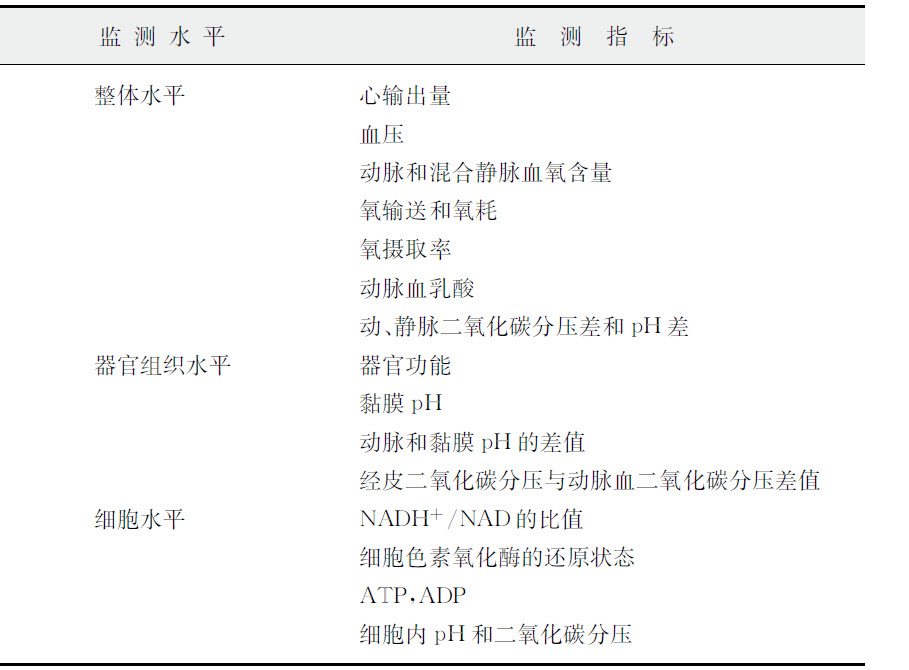
\includegraphics[width=\textwidth,height=\textheight,keepaspectratio]{./images/Image00019.jpg}\\
 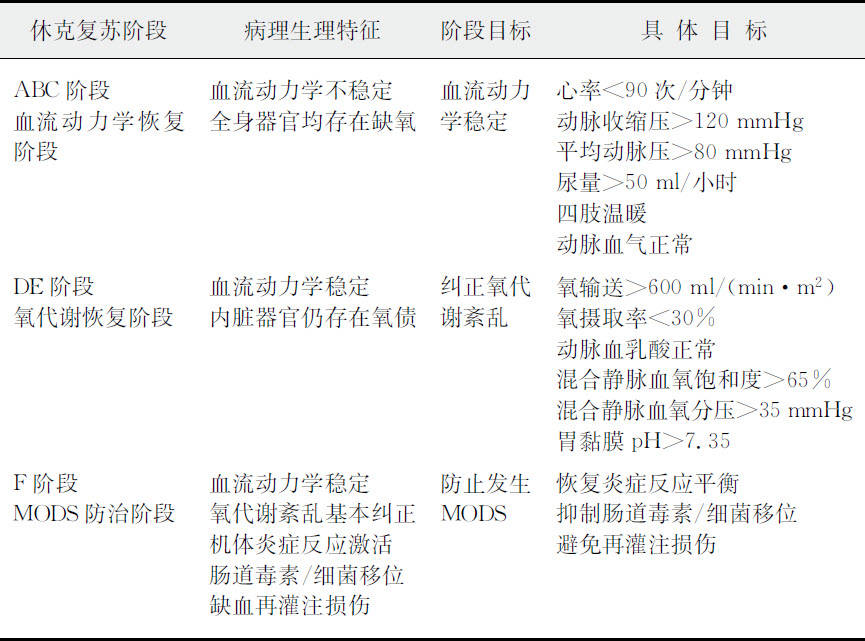
\includegraphics[width=\textwidth,height=\textheight,keepaspectratio]{./images/Image00020.jpg}
 \end{longtable}

\subsection{一、感 染}

感染是长期发热最常见的原因。在各种感染中,结核病是主要原因之一,特别是某些肺外结核,如深部淋巴结结核、肝、脾结核尤难于诊断;早期的急性粟粒型结核和脊椎结核也难于诊断。

其他感染还有伤寒与副伤寒、亚急性感染性心内膜炎、布鲁菌病、败血症、阿米巴肝病、CMV病毒、HIV、真菌等。

\subsection{二、血液病}

不明原因发热中以淋巴瘤所占比例最高,常成为诊断难题。

发热、出血、进行性贫血,肝、脾、淋巴结肿大,可提示血液病诊断的线索。

\subsection{三、风湿性疾病}

风湿性疾病的临床表现多种多样,其中,发热可以为首发症状,亦可在病程中出现。有报道各种风湿性疾病出现发热的几率排列为:Still病100\%,SLE
70\%~80\%,干燥综合征20\%,肌炎及(或)皮肌炎10\%,系统性硬皮症约5\%。其中Still病约占结缔组织病发热的50\%。临床上两个以上互不相关的器官损害表现可提供结缔组织病的诊断线索,其中以多发性关节炎与皮疹是最常见的共同表现,且往往早期出现,还可出现心、血管、肝、肾、肺、肌肉等器官和组织的损害。其实验室检查的特点是自身抗体及高免疫蛋白血症。

\subsection{四、恶性肿瘤}

恶性肿瘤生长迅速,当肿瘤组织崩溃或合并感染时则可引起长期发热。如肝癌、结肠癌,早期易漏诊。血清乳酸脱氢酶活性、癌胚抗原(CEA)、甲胎蛋白(AFP)等测定有助于诊断。

李龙芸回顾了1953-1997年《中华内科杂志》刊出的124例病例的临床病理(例)讨论见表\ref{tab2-15}及表\ref{tab2-16},确诊方法:尸检85例,开胸探查5例,开腹探查11例,组织活检15例及实验室检查8例。疑难发热病病因以感染性、血液系统及肿瘤疾病为主,分别为36.4\%、30.2\%及20.9\%。感染性疾病中以细菌性及结核性感染为主,其次为病毒性、寄生虫性及霉菌性感染。血液性疾病中以淋巴瘤、恶性组织细胞病为主。结核性疾病及寄生虫感染无减少趋向,病毒及霉菌性感染报道增多,尤其艾滋病、卡氏肺孢子菌肺炎及巨细胞病毒。对疑难发热病例应警惕结核、细菌性感染及寄生虫、淋巴瘤、恶性组织细胞病、恶性肿瘤等。这组患者结核病以中青年为主,热程1~18个月,平均(6.1±5.7)个月。淋巴瘤大多数热程超过1年。恶性组织细胞病10天~3年,平均(6.2±5.7)个月。成人Still病热程1个月~1年,平均5.3个月。

1998-2013年《中华内科杂志》刊出长期不明发热的临床病例讨论29例的病因见表\ref{tab2-17},29例中淋巴瘤占45\%。

\begin{table}[htbp]
\centering
\caption{1953-1997年《中华内科杂志》刊出的47例疑难临床病理讨论的感染性疾病发热的病因}
\label{tab2-15}
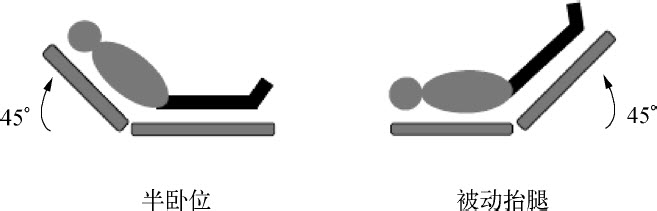
\includegraphics[width=5.94792in,height=3.83333in]{./images/Image00021.jpg}
\end{table}

\begin{table}[htbp]
\centering
\caption{1953-1997年《中华内科杂志》刊出发热疑难临床病理讨论的肿瘤、血液、结缔组织病性疾病}
\label{tab2-16}
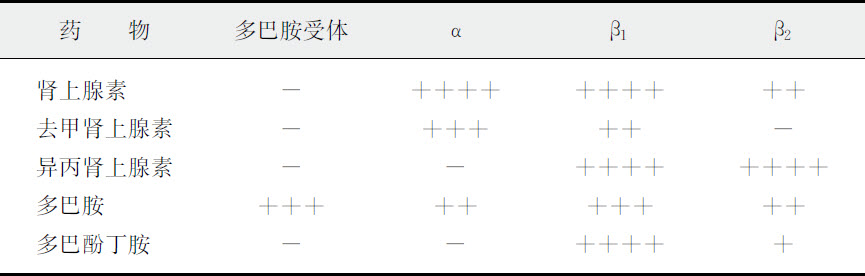
\includegraphics[width=5.95833in,height=4.41667in]{./images/Image00022.jpg}
\end{table}

\begin{table}[htbp]
\centering
\caption{1998-2013年《中华内科杂志》刊出长期不明发热的临床病例讨论29例的病因}
\label{tab2-17}
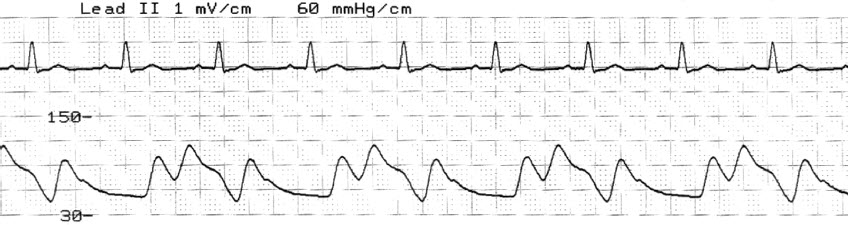
\includegraphics[width=5.95833in,height=2.92708in]{./images/Image00023.jpg}
\end{table}

另有报道一组未明原因长期发热449例(表\ref{tab2-18})。病因包括:感染性疾病(56.8\%),其中结核病占43.6\%;且以肺外结核居多,肺外结核临床表现复杂多样,但大多数患者除长期发热外,常伴乏力、纳差、盗汗、消瘦等结核中毒症状,随着病情进展,有些可出现结核感染部位的症状,也可有血沉增快、γ-球蛋白比值升高、结核菌纯蛋白衍生物(PPD)阳性。一般抗生素治疗无效,需特异性抗结核治疗才有效。PPD强阳性有助于结核病的诊断,但其阴性也不能除外结核诊断。本组有1例腰椎结核患者在院外误诊达15个月之久,故需提高对肺外结核的认识。

此组疾病中结缔组织病19.6\%,其中成人Still病34.6\%,是结缔组织病中引起长期不明原因发热的主要病因。

肿瘤性疾病16.5\%,其中淋巴瘤39.1\%;诊断最困难,因此如怀疑本病建议多次行淋巴结活检,局限于上消化道的淋巴瘤可做胃镜及活检,腹腔内淋巴瘤必要时手术探查,尽早明确诊断,及时治疗。

其他疾病7.1\%,其中坏死性淋巴结炎占33.3\%,药物热占26\%;出院时仍未确诊13.8\%。

\protect\hypertarget{text00033.html}{}{}

\subsection{5.1 感染性疾病}

\subsubsection{一、结核病}

结核病是感染性疾病中引起不明原因长期发热的主要原因。马小军等在2004年的研究显示,449例FUO患者中结核病占21.4\%。侍效春等报道不明原因发热为表现的100例结核病中,可以中高度发热,热型以不规则热为多见,弛张热、稽留热次之,39\%患者有寒战,热程3~77周,中位热程为12周。结核累及部位:单纯肺结核39例,单纯肺外结核28例包括腹腔结核(肠结核、结核性腹膜炎、肝结核、腹腔淋巴结结核)11例、淋巴结(颈部、腹股沟、纵隔)结核4例、结核性心包炎2例、结核性脑膜炎2例及无明确部位9例,肺结核合并肺外结核33例,50\%患者PPD皮试阳性,实验室检查多为ESR增快和C反应蛋白升高以及不同程度的消耗表现即贫血和低白蛋白血症,诊断方法:抗酸杆菌阳性的34例,组织病理符合结核病的8例,临床诊断并经抗结核治疗有效的49例,诊断性抗结核治疗有效的9例。接受抗结核治疗后显效的时间平均为5.3周。从发病至确诊的时间为3~77周,中位确诊时间14周。诊断性抗结核治疗依旧是目前诊断肺外结核的主要方法。对结核病高度可疑病例的诊断性抗结核治疗观察时间放宽到8周,较广为采用的期限4~6周为宜。

\begin{table}[htbp]
\centering
\caption{449例不明原因长期发热的病因分类}
\label{tab2-18}
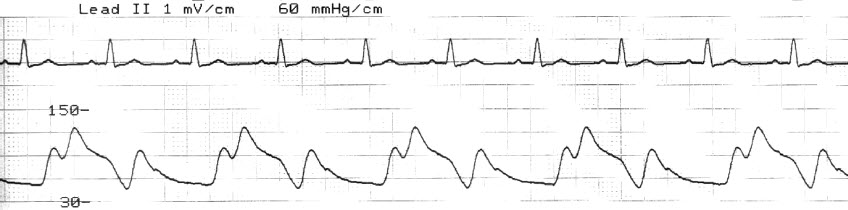
\includegraphics[width=5.97917in,height=8.40625in]{./images/Image00024.jpg}
\end{table}

\paragraph{(一)急性粟粒型肺结核}

过分相信X线胸部透视的阴性结果,可能漏诊急性粟粒型肺结核。易致漏诊或误诊为伤寒型粟粒型肺结核。一个类似伤寒的患者,而有脉快、呼吸迫促、轻度发绀、血象白细胞减少(但也可增多)兼有淋巴细胞减少,体格检查未发现明显的心肺体征,应考虑急性粟粒型肺结核的可能性。此病以儿童及青年人为多见,但中年以上也可罹患。虽然一次胸部照片阴性,对怀疑病例需隔1~2周再作胸片复查。

\paragraph{(二)肝结核}

肝结核的患者大多数存在肝外结核病灶,部分可以没有肝外病灶。在血源性播散时结核杆菌经肝动脉而进入肝脏,若继发于胃肠道结核病灶则可经门静脉系统而进入肝脏。肝结核临床上少见,由于缺乏典型症状,诊断较为困难,在未确诊之前临床表现不易与淋巴瘤相鉴别。

值得注意的是所谓“原发性”肝粟粒性结核,此病一般常规检查难以发现其他结核病灶。此种病例甚为罕见,诊断极困难。国外文献提到“原发性”肝粟粒性结核的下列诊断依据可供参考:①原因未明的发热;②肝大,不一定伴有压痛;③脾大;④关节痛或皮疹;⑤腹部胀满而躯体消瘦;⑥腹水的蛋白含量高于4g\%;⑦未能解释的血沉加快、中等度贫血与白细胞减少;⑧未能解释的血清球蛋白增加;⑨阳性的结核菌素试验。患者大多具有上述表现的大部分或全部。此病多见于青壮年人,发热可迁延甚久。CT肝扫描可发现肝粟粒病灶,确诊须依靠肝穿刺活检。笔者见女性,60岁,反复中高发热9个月,全血细胞减少,总胆红素104μmol/L,结合胆红素79μmol/L,非结合胆红素25μmol/L,转氨酶升高,纤维蛋白原低,凝血酶时间延长,胸片示右肺尖少许陈旧性结核,PPD皮试阴性,腹部CT:肝不大,脾稍大,在B超引导下进行肝穿刺活检,考虑为(肝脏)结核,经抗结核治疗好转出院。

\paragraph{(三)脾结核}

多见于青壮年,表现为长期发热、弛张热、左上腹不适、脾大,可无脾外结核表现,结核菌素试验不一定阳性,B超或CT示脾内多发或单发低密度灶,CT增强后病灶无强化。不易与脾型淋巴瘤鉴别,唯有病理检查有助诊断。可行B超引导下脾穿刺活检或脾切除术。

\paragraph{(四)深部淋巴结结核}

需注意肠系膜淋巴结结核。此病多侵犯儿童与青少年,但中年以上偶患。主要症状是长期发热、与饮食无关的腹部钝痛、消瘦、盗汗等。如有肠粘连,可引起剧烈的肠绞痛。热型为弛张型或不规则型,体温可高达39℃以上,但也可为微热。血沉常明显加快,也无蔷薇疹与脾大。在病程经过中有时触及淋巴结团块,CT检查有时误诊为腹部淋巴瘤或腹腔内其他恶性肿瘤。腹部平片可发现肠系膜淋巴结钙化影像。B超引导下包块穿刺或腹腔镜检查取淋巴结活检对诊断有很大的帮助,若无条件做检查,如患者有结核病接触史或伴有其他器官的结核病,宜试行抗结核治疗,从疗效上证实对结核病的臆断;如诊断性治疗无效,可考虑剖腹探查。

其他:无反应性结核常见于器官移植术后或严重免疫抑制患者。笔者见1例无反应性结核,患急性淋巴细胞白血病行异基因干细胞移植6个月后出现长期高热,伴有血性胸水或血性心包积液,肺部无结核表现,结核菌素试验阴性,未找到结核杆菌,血象白细胞升高达(70~80)×
10\textsuperscript{9} /L,继而下降至1×10\textsuperscript{9}
/L以下,血小板≤20×10\textsuperscript{9}
/L,中、重度贫血。骨髓呈大量中性中幼粒细胞类白血病反应。这种患者试验性抗结核治疗往往作为结核鉴别诊断的方法之一。

\subsubsection{二、感染性心内膜炎}

感染性心内膜炎是长期不明原因发热的病因之一,对于长期不明发热患者,需要询问既往有无器质心脏病,并仔细听诊心脏杂音,发热若有心脏杂音、周围动脉栓塞、皮肤黏膜瘀点、贫血、脾大、应考虑本病的可能,也有缺乏心脏杂音如感染累及心脏右侧杂音,易被漏诊。超声心动图及血培养可帮助诊断。但约有7\%~28\%的感染心内膜炎血培养阴性,可能由于之前多已应用抗生素;培养方法不当;特殊感染如立克次体、真菌。心内膜炎的诊断标准见第1.1.2节中“感染性心内膜炎”部分。

近年来由于某些诊疗技术的应用增多,如漂浮导管放置时间太长、血液透析、静脉高营养治疗和静脉吸毒等,致感染性心内膜炎发病有所增加,国内报道致病菌以草绿色链球菌为多,长期用药者则以金黄色葡萄球菌为常见,其次为铜绿假单胞菌(绿脓杆菌),也有的为真菌。

\subsubsection{三、败血症}

败血症也是长期发热的常见原因之一。国内报道病原以金黄色葡萄球菌最多,大肠杆菌次之,其他细菌少见。败血症消除后患者仍可能有发热。此类长期发热原因最多为迁徙性化脓病灶,可位于体内任何组织和器官。有的深在病灶,须用影像学检查(如B超、CT)以证明之。其次为所谓“后继热”,有认为与感染消除后,体温调节中枢功能尚未稳定有关,一般为微热,少数为药物热,多伴有药疹,停用有关药物后体温复常。

\subsubsection{四、伤寒、副伤寒}

伤寒、副伤寒甲常为长期不明发热原因之一,造成诊断困难的原因是伤寒患者缺乏中毒症状,相对缓脉、典型皮疹、肥达反应缺乏特异性,也易出现阴性。

\subsubsection{五、获得性免疫缺陷综合征(艾滋病)}

由人类免疫缺陷病毒(HIV)引起,一旦进入AIDS期,常见症状有发热、咳嗽、咳痰、气短、低氧血症、乏力、消瘦、全身淋巴结肿大,反复肺和肠道感染,抗感染无效。有些患者贫血、白细胞减少、血小板减少,可以两系或三系减少。与肺间质纤维化、结节病、结核有时难以鉴别,要反复测定HIV抗体,一旦阳性,应进一步作蛋白印迹法以确证是否HIV感染。

\subsubsection{六、其他病毒性疾病}

病毒性疾病一般病程自限,EB病毒和巨细胞病毒感染可作为长期发热的病因,诊断主要依据为分离到病毒,或血清学相应抗原或特异性IgM抗体检测。虽有自限性的特点但病程迁延(5~8周),血白细胞变化特点是计数轻微升高或正常而淋巴细胞比例显著增加,有肝功能异常等多脏器受累的表现,严重者甚至出现横纹肌溶解、肾功能异常。

\subsubsection{七、侵袭性真菌病}

恶性肿瘤患者放疗、化疗后中性粒细胞减少;器官移植或免疫性疾病需要长期使用糖皮质激素或免疫抑制剂;ICU患者、HIV感染者、反复使用广谱抗生素者、慢性消耗性疾病等,上述患者出现长期发热应想到真菌感染的可能。主要致病菌有念珠菌、曲霉、隐球菌、毛霉等。曲霉病的发病有上升趋势。感染部位有内脏感染:肺、肝、脾、脑、肾、组织;全身播散:真菌败血症,其中侵袭性肺曲霉病最常见。真菌感染患者除了发热外,局部症状不明显,不及时治疗死亡率高。对于存在真菌感染高危因素的患者出现不明原因发热,需行胸部CT检查;体液(痰、尿、血)真菌培养,血培养受多种因素影响,阳性率低;葡聚糖检测(G试验)、半乳甘露聚糖抗原检测(GM试验);确诊需要侵入性的组织活检,但在状况很差的患者难实施,所以确诊困难,大多数属于临床拟诊或临床诊断。往往需要试验性治疗。血液系统恶性肿瘤患者若粒细胞减少(≤0.5×10\textsuperscript{9}
/L),不明原因发热(体温>38℃),96小时广谱抗生素治疗无效时,可进行经验性使用伏立康唑或伊曲康唑、棘白菌素如卡泊芬净、米卡芬净抗真菌治疗。

组织胞浆菌病 是一种较少见的由荚膜组织胞浆菌引起的深部真菌感染性疾病。局限性感染可无临床症状或表现为亚临床型,播散型组织胞浆菌病可累及单核巨噬细胞系统及全身脏器,如肝、脾、骨髓、淋巴结等。当吸入本菌的孢子,进入肺泡,被巨噬细胞吞噬,再通过网状内皮系统进行全身播散。疾病的严重程度取决于吸入孢子量及宿主自身免疫反应。播散型常见于长期使用糖皮质激素等免疫功能低下者,临床表现为长期高热,肝、脾、淋巴结肿大,全血细胞减少,肝酶尤其ALP升高常见。涉及胃肠道感染的可以表现为腹泻及腹痛,部分可合并噬血细胞综合征。重症者可以合并DIC,急性肾衰;易误诊为淋巴瘤、结核病。

确定诊断需做真菌检查:①骨髓涂片:可见巨噬细胞内大量卵圆形吞噬体,紫红色半月形胞质集中在吞噬体的一端,外周围绕未染色的空晕,形似荚膜。②真菌培养:通常所需时间为4~6周,形态学上具有结节大孢子是组织胞浆菌的特征。镜下组织胞浆菌典型形态为2~4μm椭圆形芽生酵母,以能被亚甲胺银染色及过碘酸-schiff(pas)染色为特征,当为进行播散型组织胞浆菌时,可在血液细胞中发现其孢子。③组织胞浆菌多糖抗原检测往往在尿液、体液中检测,在播散型组织胞浆菌中起着快速诊断作用,但容易产生假阳性,特别注意与芽生菌鉴别。组织胞浆菌需与马尔尼菲青霉菌、黑热病鉴别。

\subsubsection{八、布鲁菌病}

布鲁菌病(Brucellosis,布病),也称波状热,是由布氏杆菌引起的急性或慢性人畜共患性传染病,此病在国内多见于内蒙古、东北、西北等牧区,牧民、兽医、屠宰工人和炊事员的发病率较高。非疫区偶也有报道。饮用污染乳品也可引起感染。

布鲁菌病临床表现缺乏特异性,发热可以持续数日乃至数周以上,多数为高热、多汗、关节痛、疲乏、睾丸炎、淋巴结与肝脾大,部分患者有贫血、轻度白细胞减少,红细胞沉降率加快。实验室检查:①血液或骨髓培养:分离到布氏杆菌;②血清学检查:虎红凝集试验,试管凝集试验阳性;凝集反应通常于病期第一周后开始出现,但也可较晚,滴度在1∶100以上方有诊断价值,1∶200~400为阳性,1∶800以上为强阳性。如滴度过低,应隔一周或更长时间复查。有的病例滴度可不高,甚至呈阴性反应。血清凝集反应阴性的病例,血及骨髓培养均可出现阳性(分别为33.3\%与57.1\%)。羊型波状热病例的血培养与骨髓培养阳性率甚高(80\%)。因此如在流行疫区临床表现符合而血清凝集反应阴性,不能轻易除外此病的可能性。左氧氟沙星、利福平、多西环素抗感染有效,疗程需达6周。

布鲁菌病由于发病率低,有时接触史不明显,全身症状无特异,不易引起临床医师的重视,易导致漏诊和误诊。非疫区若饮用污染乳品出现长期不明原因发热,需做培养、血清学检查排除该病。

\subsubsection{九、阿米巴肝病}

阿米巴肝病,早期难于诊断,也易于漏诊。另一方面由于抗生素(红霉素、四环素族)的广泛应用于一般感染性发热疾病,也可使阿米巴肝病呈较为缓和的经过,而易于忽略。因此,患者有长期原因未明的发热、肝大、血象白细胞数轻度或中等度增多,不论有无肝区疼痛和过去有无痢疾史,必须考虑此病的可能性(参见有关章节)。

\subsubsection{十、黑热病}

黑热病即内脏利什曼病,是由杜氏利什曼原虫引起、通过白蛉传播的慢性地方性传染病,黑热病有严格的地区性。本病在新中国成立以来经多年大力防治,已基本消灭。近年来,甘肃、四川、新疆、内蒙古及山西等地区出现散发病例,随着经济与人员流动的全球化趋势,地方性传染病病例可能在一些传统理论中的非流行区出现,即在非疫源性地区,也偶见有散发病例报道,实验室检验人员对利什曼原虫形态不熟悉,易被误诊或漏诊。

该病各年龄均可发病,可表现为长期不明原因发热,早期病例约1/3呈双峰热型,可有畏寒,寒战,肝脾大,少数有巨脾、全血细胞减少、消瘦、进行性衰竭,骨髓易见组织细胞,在非疫区的医院就诊,易误诊为恶性组织细胞病,淋巴瘤。该病葡萄糖酸锑钠治疗有效。

对于患者长期发热原因未明而兼有肝脾大、血细胞减少等,需仔细追问是否去过疫区,须注意罕见病黑热病的可能性。黑热病的确诊须依靠以下的实验室检查:①血免疫层析试条(rK39dipstick)法检测:血清黑热病抗体阳性。②寻找黑热病原虫:骨髓穿刺发现黑热病原虫是最确实的诊断方法。在不同部位进行反复的骨髓穿刺,累积的阳性率颇高。瑞氏染色形态需与组织胞浆菌病、马尔尼菲青霉菌病鉴别,黑热病糖原染色胞内容物为红色,而后两者胞内容物不着色。

\subsubsection{十一、人粒细胞无形体病}

急性不明原因发热需注意罕见病、新发现的立克次体传染病,人粒细胞无形体病(human
granulocyticanapasmosis,HGA),是由嗜吞噬细胞无形体引起的一种经蜱传播的立克次体病,1992年在美国明尼苏达州发现HGA,且多为个例或散发流行,HGA是一种以粒细胞为主要靶细胞,常累及全身多个脏器,临床表现多样且凶险的疾病。近几年在我国江苏、湖北、河南、安徽等曾有类似疫情发生的病例报道。

HGA潜伏期一般为7~14日(平均9日),常急性起病,主要表现为不明原因发热(多为持续性高热,可高达40℃以上)、乏力、头痛、肌肉酸痛,约一半患者有消化道症状等。部分患者伴有咳嗽、咽痛,可出现意识障碍。体检可见表情淡漠,相对缓脉,少数患者可有浅表淋巴结肿大及皮疹。严重者可出现感染中毒性休克、肝炎、心肌炎、急性肾衰竭、呼吸窘迫综合征、弥散性血管内凝血(DIC)及多脏器功能衰竭等。

该病的诊断主要依据:①流行病学史:发病前2周内有被蜱叮咬或接触暴露史;在有蜱活动的丘陵、山区(林区)工作或生活史;或直接接触过危重患者的体液等。②临床表现:急性起病,主要症状为发热(多为持续性高热,可高达40℃以上)、全身不适、乏力、头痛、肌肉酸痛,以及恶心、呕吐、厌食、腹泻等。个别重症病例可出现皮肤瘀斑、出血,伴多脏器损伤、DIC等。③实验室检查:早期外周血白细胞、血小板降低,严重者呈进行性减少,异形淋巴细胞增多;外周血涂片瑞士染色镜检中性粒细胞内可见桑葚状包涵体;ALT/AST升高。急性期血清间接免疫荧光抗体(IFA)检测嗜吞噬细胞无形体IgM抗体阳性(抗体滴度≥1∶256)或急性期与恢复期双份血清IgG抗体呈4倍升高。全血或血细胞标本PCR检测嗜吞噬细胞无形体特异性核酸阳性,或分离到病原体。该病首选强力霉素治疗,有禁忌证者可选用利福平或喹诺酮类。

\protect\hypertarget{text00034.html}{}{}

\subsection{5.2 血液病}

淋巴瘤是引起长期不明原因发热最常见的恶性肿瘤。

\subsubsection{一、恶性淋巴瘤}

恶性淋巴瘤是恶性肿瘤性长期不明原因发热的主要病因,占首位(50\%)。恶性淋巴瘤是一组起源于淋巴结或其他淋巴组织的恶性肿瘤,可发生于人体内任何器官与组织,病理类型在我国以非霍奇金淋巴瘤(NHL)居大多数,霍奇金淋巴瘤(HL)仅占8\%~11\%。

以长期发热为主要和首发表现的淋巴瘤常见,临床表现复杂,尤其对那些浅表淋巴结无肿大,病灶在深部淋巴组织器官的淋巴瘤(原发于胃肠道、肺、肝、脾、骨髓、多浆膜腔、中枢神经系统、脊柱等任一部位病变),易误诊。结外病变有:①胃肠道以小肠为多,其次为胃,结肠很少受累。②胸部以肺门及纵隔受累最多,半数有肺部浸润或(及)胸腔积液。③肝、脾大。④骨髓累及者约占1/3~2/3。⑤骨骼以胸椎及腰椎最常见,股骨、肋骨、骨盆及头颅次之。⑥皮肤受累表现为肿块、皮下结节、斑块、溃疡等。⑦其他部位如鼻咽、乳腺、甲状腺、眼眶、肾上腺、肾脏、睾丸、中枢神经系统、生殖系统等均有可能受累。

淋巴瘤发热特点:

(1)发生率:淋巴瘤以发热为主要或首发症状者约占16\%~30\%,霍奇金淋巴瘤在病程早期有发热表现者可占30\%~50\%,非霍奇金淋巴瘤(NHL)约占24\%左右。NHL在病变较广泛或深部病变时更易有发热表现,侵犯到骨髓的NHL
80\%的患者均有发热表现。

(2)热型:约1/6的霍奇金淋巴瘤出现周期性热。NHL的热型呈弛张热、周期热或不规则热。

(3)热程长:有些病例待明确诊断,病程已达数月甚至达1年以上。有报道53例不明原因发热为首发的淋巴瘤,从发病到确诊的平均时间为35(5~184)周,其中大于1年病程10例。

(4)有的毒血症的表现常不明显。

(5)T-NHL比B-NHL更易有发热,有文献报道中、高度恶性T-NHL的发热为77.5\%,而B-NHL为22.4\%,尤其是皮下脂膜炎样T淋巴瘤、NK/T细胞淋巴瘤、肝脾γ/δT细胞淋巴瘤、血管免疫母细胞型T细胞淋巴瘤和间变性大细胞型(CD30\textsuperscript{+}
)淋巴瘤或称Ki-1\textsuperscript{+}
淋巴瘤、淋巴瘤性的噬血细胞综合征这些特殊类型多见有发热。

(6)抗感染治疗无效,部分应用糖皮质激素,体温可降至正常,也有用糖皮质激素无法退热。

(7)有些病例至晚期才出现肝、脾大、腹腔淋巴结肿大,白细胞减少、贫血或全血细胞减少。

对于长期不明原因发热而不能以感染性疾病、结缔组织病解释者,X线、B超、CT、MRI及正电子发射型断层扫描技术(PET)等寻找体内肿大的淋巴结和病变,尤其PET-CT对以长期发热为主要表现的淋巴瘤的筛查有价值,可以显示病灶及代谢异常,对穿刺活组织检查有定位价值;有报道的15个(723例患者)关于淋巴瘤PET
FDG显像结果进行总结,PET
FDG显像的敏感性为71\%~100\%,特异性为69\%~100\%,阴性预测值80\%~100\%。需要注意不同亚型的淋巴瘤阳性检出率不同,对弥漫性大B细胞淋巴瘤(DLBCL)、套细胞淋巴瘤(MCL)和滤泡性淋巴瘤(FL)等常见的亚型阳性检出率较高,而对淋巴结边缘区淋巴瘤(MZL)、黏膜相关性淋巴瘤(MALL型)、结外边缘区B细胞淋巴瘤(MALT-MZL)、外周T细胞淋巴瘤和伯基特淋巴瘤(BL)等少见的亚型阳性检出率相对较低。即肿瘤太小、恶性程度低等,PET-CT检查可表现为假阴性。

病理组织学和免疫组化是确诊淋巴瘤的主要依据,所以要千方百计寻找可供活检的病灶及早进行病理检查。①有浅表淋巴结肿大者,尽量选择有意义的完整淋巴结进行活组织结构及细胞形态学的检查,通过活检很容易确诊;对较深部位的淋巴结可在B超或CT引导下经皮细针穿刺活检,淋巴结病变并非弥漫分布,必要时需多次重复活检。②对于以结外病变为主要表现的淋巴瘤,根据相应病灶部位进行组织活检。③对于长期发热、肝脾大、全血细胞减少的患者,需要反复多部位骨髓活检;骨髓流式细胞仪免疫学检查、单克隆性基因重排,如免疫球蛋白重链(IgH)基因重排和T细胞受体(TCR)基因重排对诊断有一定帮助;经过多次骨髓涂片和骨髓活检后,诊断仍不明确,在无禁忌证时,腹腔镜下或剖腹行脾切除等对淋巴瘤的诊断有极大帮助。许多临床病理讨论均为淋巴瘤,说明以FUO为首发表现的淋巴瘤仍是诊断难题。

不明原因发热为首发的淋巴瘤需与成人Still病相鉴别,对于不明原因长期发热,PET-CT无显示淋巴结及结外病灶及高代谢,排除感染性疾病、肿瘤性疾病,中小量糖皮质激素或消炎镇痛药能退热者,成人斯蒂尔病可能性大。但仍需追踪排除发展为淋巴瘤。

不明原因发热为首发的淋巴瘤也需与肺外结核相鉴别。

\subsubsection{二、恶性组织细胞病}

恶性组织细胞病(简称恶组)是异常组织细胞增生所致的恶性疾病。过去曾采用许多不同的名称,如恶性组织细胞病、网状细胞白血病。过去报道的恶组实际上大多为伴噬血细胞综合征的恶性淋巴瘤,欧美大多数为间变性大细胞淋巴瘤,而在亚洲地区多为外周NK/T细胞淋巴瘤。真正的恶性组织细胞病极少见。此病的主要表现是高热,肝、脾、淋巴结肿大,全血细胞减少及进行性衰竭,病情凶险,预后不良。

根据恶性组织细胞浸润部位的不同,临床可有不同的表现,因此临床表现多种多样:①起病急,反复发热,持续时间可达27天至4个半月以上、全身进行性衰竭。热型以不规则高热居多(38.7\%),其次为稽留热(26.3\%)、弛张热(21.72)、间歇热(10.8\%)及低热少见(3\%),血培养始终阴性,各种抗生素治疗无效,对肾上腺皮质激素类药物反应差,即使体温有下降,常不能降至正常或下降后短期又上升,且连续应用逐渐失效。②造血系统受累的表现有出血、贫血、感染,肝、脾、淋巴结肿大。可有黄疸、肝功能损害等。③其他系统浸润的表现,如多发性浆膜腔积液,皮肤、胃肠、肺、肾、神经系统浸润引起的相应临床表现。

实验室检查:

1.血象 全血细胞减少,为本病的突出表现之一。

2.骨髓细胞形态及(或)活体组织病理学检查
是诊断本病的重要依据,骨髓涂片可检出异常的组织细胞,这些细胞占有核细胞的10\%~60\%。此病的异常细胞有五种类型:①异常组织细胞;②淋巴样组织细胞;③多核巨细胞;④单核样组织细胞;⑤吞噬细胞。异常组织细胞及(或)多核巨噬组织细胞有特异性诊断价值。由于骨髓损害可能为非弥漫性,或因骨髓穿刺取材甚少或取材欠佳,只能反映很小的局部情况,故阴性时不能除外本病的存在。必要时可在不同部位穿刺检查。有些病例骨髓穿刺涂片阴性,却在尸检骨髓组织切片中发现异常组织细胞。其他部位活体组织病理检查,可行皮肤、淋巴结、肝脏、脾、骨髓活检。目前缺乏识别组织细胞的特异性抗体,通常组织化学染色显示溶菌酶染色阳性,抗胰蛋白酶阳性,α1-抗胰糜蛋白酶阳性,CD68\textsuperscript{+}
为组织细胞的标志。

对不明原因的长期发热而不能以感染性疾病解释者,尤其是伴有全血细胞减少和肝、脾、淋巴结肿大,应考虑本病可能性。结合骨髓或活体组织病理学检查找到异常组织细胞及(或)多核巨噬组织细胞,同时排除反应性组织细胞增多症和Ki-1阳性的T细胞淋巴瘤,可以确立诊断。恶性组织细胞病需与下列疾病鉴别:

1.反应性组织细胞增多症
某些疾病(例如伤寒、结核病、败血症、结缔组织病等),有时骨髓涂片检查可以有组织细胞明显增多,这种反应性组织细胞增多症与恶性组织细胞病的鉴别对治疗和预后都有极为重要的意义,但二者的鉴别有时颇为困难,表\ref{tab2-19}可供参考。

2.CD30\textsuperscript{+}
的间变性大细胞型淋巴瘤(Ki-1阳性的T细胞淋巴瘤,ALCL) 占成人NHL
的3\%,本病与恶性组织细胞病在临床上、组织病理上易发生混淆,前者从分子水平证实其属T细胞系。45\%的患者有t(2;5)(p23;q35)染色体易位;CD30阳性;60\%~85\%的患者可检测出间变性淋巴瘤激酶基因(ALK)阳性;大部分病例CD2\textsuperscript{+}
、CD4\textsuperscript{+}
、细胞毒相关抗原TIA-1、颗粒酶B阳性,而呈CD3\textsuperscript{-}
、CD5\textsuperscript{-} 、CD7\textsuperscript{-} 。而恶组则无相应改变。

\begin{table}[htbp]
\centering
\caption{反应性组织细胞增多症与恶性组织细胞病的鉴别}
\label{tab2-19}
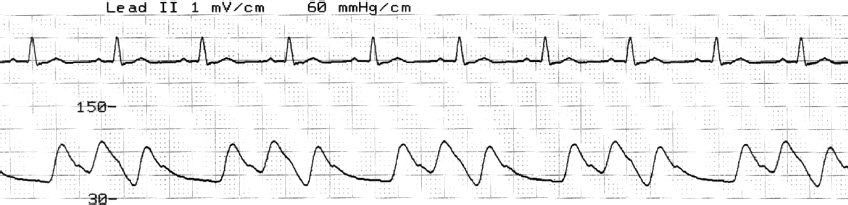
\includegraphics[width=5.90625in,height=3.02083in]{./images/Image00025.jpg}
\end{table}

\subsubsection{三、噬血细胞综合征(HPS)}

噬血细胞综合征是单核/巨噬系统反应性疾病,以组织细胞良性、大量增生,伴有明显的吞噬血细胞现象为特征。噬血综合征常常难以查出其病因,长期高热是噬血细胞综合征之一的表现,是由T细胞、巨噬细胞活化分泌IL-1、IL-6等内源性致热原而引起发热。

2004年国际组织细胞协会噬血细胞综合征的诊断标准:①发热,持续7天以上,体温超过38℃;②脾大;③全血细胞减少;④高甘油三酯血症或低纤维蛋白血症;⑤骨髓、脾、淋巴结中可见到吞噬红细胞、粒细胞或血小板的组织细胞;⑥NK细胞活性减低或缺失;⑦铁蛋白升高(铁蛋白≥3SD正常值,通常≥1000ng/ml);⑧可溶性IL-2受体(sCD\textsubscript{25}
)水平明显升高。8项中符合5项可考虑噬血细胞综合征。分遗传性和获得性,前者常发生于0~2岁的婴幼儿,后者可继发于感染(病毒尤其EB病毒、细菌、真菌、原虫)、淋巴瘤和自身免疫性疾病。其中EB病毒感染相关的噬血细胞综合征是长期不明发热的病因之一,包括EB病毒阳性的T淋巴细胞增殖症和淋巴瘤相关的噬血细胞综合征,前者血清EBV抗体滴度增高、EBDNA拷贝数升高,但淋巴结病理检查中未见典型的淋巴瘤表现,骨髓细胞也未检出克隆性T细胞受体重排。后者早期常常难以诊断,随病情进展组织活检有淋巴瘤的依据。

\subsubsection{四、急性白血病}

半数的患者以发热为早期表现。可低热,也可高达39~40℃以上,伴有畏寒、出汗等。外周血象初时有的仅有白细胞升高,红细胞、血小板数正常,易被考虑为感染性疾病。但动态观察红细胞、血小板可进行性下降。有的患者有不同程度的白血病细胞增殖浸润的表现如淋巴结肿大,肝、脾大、胸骨下段压痛,骨、关节疼痛,牙龈增生、肿胀,皮肤结节、斑块,中枢神经系统浸润的表现,睾丸浸润。血象:大多数患者白细胞增多,也有白血病数正常或减少,分类可见数量不等的原始及(或)幼稚细胞,有不同程度的正细胞性贫血,绝大多数患者血小板减少,常低于<20×10\textsuperscript{9}
/L。骨髓象是诊断急性白血病的主要依据。急性白血病患者的骨髓白血病性的原始细胞占骨髓有核细胞≥20\%。因此,凡遇有原因未明的发热伴有进行性贫血、出血者应行骨髓穿刺涂片检查以确诊。

有的患者血象呈全血细胞减少,无肝、脾、淋巴结肿大,需与急性再生障碍性贫血相鉴别。有的患者表现以出血为主,临床可与特发性血小板减少性紫癜相似,但后者以血小板减少为主,红细胞(出血严重者例外)与白细胞数不减少。

白细胞增多性急性白血病需与类白血病反应相鉴别(表\ref{tab2-20})。类白血病反应是机体受到较严重的病理损害时所发生的造血组织异常反应,其特征是外周血中白细胞数增多或(及)出现幼稚细胞,血象与白血病相似。病因以急性感染为多,其次为恶性肿瘤、急性溶血、中毒、大出血、结核病、寄生虫病等,按细胞类型可区分为中性粒细胞型、淋巴细胞型、单核细胞型、嗜酸性粒细胞型等。病因去除后类白血病反应即消除,有助于诊断。

\begin{table}[htbp]
\centering
\caption{类白血病反应与急性白血病鉴别}
\label{tab2-20}
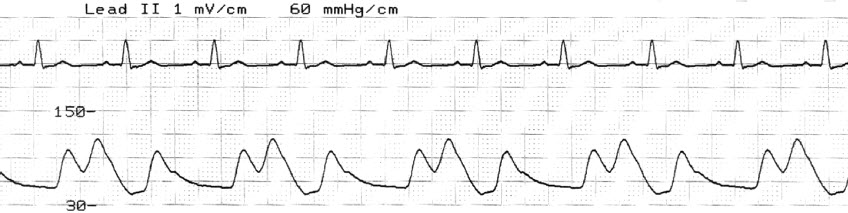
\includegraphics[width=5.91667in,height=3.875in]{./images/Image00026.jpg}
\end{table}

\subsubsection{五、组织细胞坏死性淋巴结炎}

组织细胞坏死性淋巴结炎,又称坏死性淋巴结炎、坏死增生性淋巴结病,是一种病因不明的非肿瘤性淋巴结肿大的疾病。

本病较少见,平均发病年龄30岁。起病急性或亚急性,特点如下:①95\%以上表现有发热:中、高度发热,热型呈不规则发热,也可呈弛张热,或反复间断发热,少数伴寒战,部分热程可长达2~3个月。②淋巴结肿大:多数有浅表淋巴结肿大以颈部最为常见,其次为腋窝及腹股沟,部分有压痛,也可有纵隔、腹膜后淋巴结肿大,少数有肝脾大。③少数有一过性皮疹、关节痛、多器官受累。④糖皮质激素治疗有效。

实验室检查:血象:白细胞计数常减少,可见核左移或异形淋巴细胞,轻度贫血,严重者血小板减少;对出现不明原因发热、浅表淋巴结肿大、白细胞减少,应想到本病的可能。淋巴结活检是本病诊断依据。病理学改变为淋巴结结构的部分或完全破坏,可见多少不等、大小不一的坏死灶,坏死灶周围组织细胞增多,坏死灶中可见浆细胞样单核细胞和免疫母细胞增生,无中性粒细胞浸润。由于本病的临床表现缺乏特异性,若未做淋巴结活检,误诊率高。本病需要与恶性淋巴瘤、结缔组织病、恶性组织细胞病、传染性单核细胞增多症相鉴别。

\subsubsection{六、Castleman病}

约近50\%的多中心型Castleman病表现为不明原因的长期发热,该病是一种少见的淋巴结增生性疾病,单中心型以纵隔、腹腔淋巴结肿大为多见;多中心型临床表现多样性、缺乏特异性,可以发热、浅表或深部淋巴结肿大,肝脾大,贫血,血小板减少,低白蛋白血症,免疫球蛋白升高(多克隆),易合并其他疾病或并发症如自身免疫疾病,POEMS,副肿瘤天疱疮,肾损害,淀粉样变。对疑诊本病,确诊需靠淋巴结活检病理检查,病理分为浆细胞型、透明血管型、混合型;临床分型包括单中心型、多中心型。

\subsubsection{七、朗格汉斯细胞组织细胞增生症}

一般多见于少儿,少见于成年人,临床表现:①发热:部分成年患者表现为长期发热、热型不规则,可呈周期性或持续性高热,使用抗生素无效,对激素敏感。②皮疹。③淋巴结肿大,肝、脾大。④肺部浸润:表现为轻重不等的呼吸道症状,但肺部体征不明显。肺部X线可见有弥漫性或网点状阴影。⑤骨骼破坏:长骨和扁平骨可发生溶骨性骨质破坏。⑥中枢神经系统:最常见的受累部位是丘脑-神经垂体区,弥漫性也可出现脑实质病变。有丘脑和垂体肉芽肿引起的尿崩症占该病的20\%~25\%。⑦其他:齿龈肿胀,牙齿松动,或突眼,或耳流脓或多饮多尿。病理检查是本病诊断依据,可行皮肤、淋巴结活检或病灶局部穿刺物病理检查。病理学特点是可见到特征性的分化较好的朗格汉斯组织细胞。该细胞CD1α、ATP酶、S-100蛋白、D-甘露糖苷酶均阳性。电镜下胞浆含有Birbeck颗粒。长期发热、尿崩症,要注意垂体朗格汉斯细胞组织细胞增生症。

\protect\hypertarget{text00035.html}{}{}

\subsection{5.3 风湿性疾病}

\subsubsection{一、成人斯蒂尔病}

成人斯蒂尔病(adult Still's
disease)是结缔组织病中引起长期不明原因发热的主要病因,占首位约50\%。成人Still病曾称为变异性亚败血症,是一种临床综合征。病因与发病机制尚未明确,可能与感染及自身免疫反应有关。发病年龄多于16~35岁,女性多见。表\ref{tab2-21}所示为文献报道的成人斯蒂尔病的主要临床表现。

\begin{table}[htbp]
\centering
\caption{成人斯蒂尔病的临床表现}
\label{tab2-21}
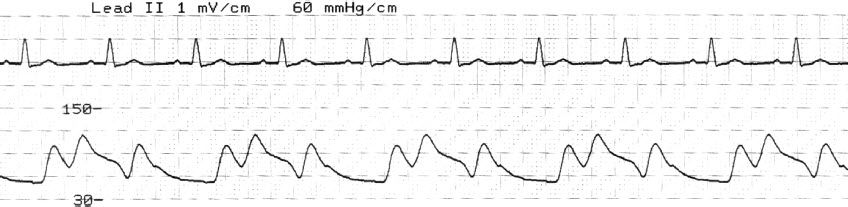
\includegraphics[width=5.9375in,height=2.29167in]{./images/Image00027.jpg}
\end{table}

\paragraph{1.临床特点}

\subparagraph{(1)发热:}

是本病的突出症状,多高于39℃,多数弛张热,也有不规则热,稽留热。热程1个月至1年,有报道平均5.3个月,常伴畏寒,但罕见有寒战,热程虽长,病情一般尚好,中毒症状不明显。各种抗生素治疗无效,而用糖皮质激素或非甾体类抗炎镇痛药能使体温降至正常。

\subparagraph{(2)皮疹:}

多为点状红疹,有时为斑丘疹或结节红斑,呈一过性,高热时出现,热退时消失。主要分布在躯干、四肢、手掌、足底。

\subparagraph{(3)关节痛或关节炎:}

可单关节或多关节受累。有时只有轻微关节痛。

\subparagraph{(4)其他:}

患者有咽痛,这是本病特征之一。部分有淋巴结肿大、肝脾大、胸膜炎、腹膜炎、心包炎、神经系统及呼吸系统损害等。除发热外有些患者起病时并非全部表现出上述症状,可能在病程中需要数月以至数年,才表现出来,亦可能始终未全部表现。

\paragraph{2.实验室检查}

(1)外周血白细胞总数增多,中性粒细胞核左移。

(2)血沉增快,C反应蛋白和免疫球蛋白升高。

(3)血清铁蛋白(SF)明显升高,铁蛋白>1000ng/ml(正常值上限的3倍)对诊断成人斯蒂尔病(AOSD)具有较高的阳性预测值(95.2\%),如果SF<1000ng/ml,则95.2\%认为不是AOSD;SF>1500ng/ml(正常值上限的5倍)阳性预测值为85.7\%,提示有临床表现者应高度怀疑AOSD。

(4)骨髓呈感染性骨髓象。

(5)2/3患者肝功能异常。

目前常用的诊断标准有日本成人Still病研究委员会制订的标准即Yamaguchi标准(1992):

主要指标:发热≥39℃,并持续1周以上;关节痛持续2周以上;典型皮疹;白细胞增高≥10×10\textsuperscript{9}
/L。

次要指标:咽喉痛;淋巴结肿大及(或)脾大;肝功能异常;类风湿因子和抗核抗体阴性。

符合5项条件含2项主要条件,排除感染性疾病及恶性肿瘤即可诊断。不典型的病例可无关节痛,一过性皮疹亦被疏漏。对于不典型病例必须充分排除其他引起长期发热的疾病才能诊断。

对诊为本病的患者必须长期随访,少数以后发展为淋巴瘤。

\subsubsection{二、系统性红斑狼疮}

长期的非感染性发热,兼有两个器官(如肾脏+浆膜;肾脏+关节;肝脏+心脏;关节+中枢神经系统)或多个器官受累的表现;发热伴血象白细胞减少、血小板减少、贫血或溶血性贫血者,应考虑系统性红斑狼疮(SLE)的可能。此病多见于女性,发病年龄多在21~40岁之间。以发热为主要临床表现者约占60\%~80\%。可以中、高热也可呈低热。首发症状的发热,伴皮疹与关节痛为多见。皮疹呈多形性,可从轻微的红斑乃至急性丹毒样病变或大疱,多见于面、颊、鼻、前胸、手、足等暴露处,但典型而有诊断价值的皮疹是蝶形红斑和盆状红斑。面部蝶形红斑虽为此病的特征性表现,但又非经常出现,国内报告阳性率为60\%~80\%。由于SLE症状复杂,如仅注意个别器官病变化,易误诊为风湿热、心包炎、胸膜炎、肾炎、类风湿关节炎、肝炎、特发性血小板减少性紫癜,甚至精神病等疾病。

美国风湿病学会1982年的SLE分类标准,对诊断SLE很有价值:①蝶形红斑:平的或高于皮肤的固定性红斑;②盘状红斑:面部的隆起红斑,上覆有鳞硝;③光过敏:日晒后皮肤过敏;④口腔溃疡;⑤关节炎:非侵蚀性关节炎;⑥浆膜炎:胸膜炎或心包炎;⑦肾病变:蛋白尿>0.5g/d或细胞管型;⑧神经系统病变:癫痫发作或精神症状;⑨血液系统异常:溶血性贫血或白细胞减少或淋巴细胞绝对值减少或血小板减少;⑩免疫学异常:狼疮细胞阳性或抗ds-DNA或抗Sm抗体阳性或梅毒血清试验假阳性
;\textcircled{11}
抗核抗体阳性。在上述11项中,如果有4项阳性,则可诊断为SLE,其特异性为98\%,敏感性为97\%。

SLE血清抗核抗体(ANA)是筛选结缔组织病的主要试验,阳性率达95\%~100\%,但特异性较差,其他结缔组织病、慢性活动性肝炎等均可呈阳性,诊断须结合临床与其他检查。血清抗双链去氧核糖核酸抗体(ds-DNA)特异性较高,且疾病早期即可出现,阳性率约62\%。抗Sm抗体是诊断SLE的标记抗体之一。特异性达99\%,但敏感性仅25\%。

系统性红斑狼疮样病象可由某些药物引起,称药物性狼疮综合征。可引起此综合征的药物可分为两类:①可引起红斑狼疮综合征的;②可使系统性红斑狼疮症状恶化的。属于第一类的药物有酰肼类药物(肼屈嗪、异烟肼等)、抗癫痫药物(如苯妥英钠)、普鲁卡因胺等。后者血清抗核抗体阳性率高达50\%~68\%,停药后症状在数周内消退,但血清抗核抗体阳性率可持续数月。此类药物性狼疮综合征罕有发生肾脏病变,且停药后不致再发。属于第二类的药物有青霉素、磺胺类、口服避孕药等,可使系统性红斑狼疮患者的症状恶化;但对正常人不致引起系统性红斑狼疮的病象或血清抗核抗体阳性。

\subsubsection{三、结节性多动脉炎(PAN)}

此病临床上少见,是一种累及中、小动脉的坏死性血管炎。此病的病理特点是多器官损害,主要累及心、肾、肺、肌肉、皮肤、关节等器官。患者以男性为多,年龄多在40~50岁之间,发热是最常见的症状,可高热也可低热。系统症状取决于受累器官。①皮肤表现:25\%~52\%患者有如血管性紫癜、结节红斑样皮肤结节、网状青斑、远段指(趾)缺血或坏死及雷诺现象;②关节肌肉表现:46\%~63\%患者可有关节炎、多发性肌痛和间歇性跛行;③神经系统表现:36\%~72\%患者有神经系统受累,以外周神经受累为主;④肾表现:45\%~83\%患者出现不同程度的肾损害,主要表现为蛋白尿,血、尿、细胞管型,高血压;⑤其他表现如胃肠道、心脏、肺、生殖系统等受累则有相应表现。

凡原因未明的长期发热,兼有多个互不相关的器官受累的表现,血象白细胞增多,须考虑此病的可能。实验室检查一般无特异性,可见轻度贫血、白细胞轻度升高,可见蛋白尿、血尿、管型尿,C反应蛋白增高,球蛋白升高,ANCA阴性,部分病例HBsAg阳性。诊断主要根据病理活检和血管造影。可行皮肤、肌肉、肾组织或睾丸活检。血管造影常见有肾、肝、肠系膜及其他内脏器官的中、小动脉有微小动脉瘤形成和节段性狭窄。1990年美国风湿病学会关于结节性多动脉炎的分类标准见表\ref{tab2-22},在10项中有3项阳性者排除其他结缔组织病并发的血管炎即可诊断。

此病在鉴别诊断上须多注意败血症、腹腔内恶性肿瘤、心肌炎、急性白血病、皮肌炎、系统性红斑狼疮、白塞病等疾病。

\subsubsection{四、肉芽肿性多血管炎(Wegener肉芽肿)}

Wegener肉芽肿是一种系统性、坏死性肉芽肿血管炎,主要累及上、下呼吸道及肾,同时也累及全身小动脉、静脉及毛细血管。本病临床上少见,无性别差异,以40~50岁为多见。

临床表现:①全身非特异症状如发热、关节痛、肌痛;②上呼吸道:表现为鼻、中耳、鼻窦的炎症;③肺部表现:肺病变见于70\%~80\%患者,可有咳嗽、咯血、胸痛和呼吸困难。X线示中下肺野结节和浸润或空洞;④肾病变:在病程中出现不同程度的肾小球性肾炎,重者可因进行性肾病变导致肾衰竭;⑤其他表现:部分有眼、皮肤、心脏受累的相应表现。

\begin{table}[htbp]
\centering
\caption{美国风湿病学会关于结节性多动脉炎的分类标准}
\label{tab2-22}
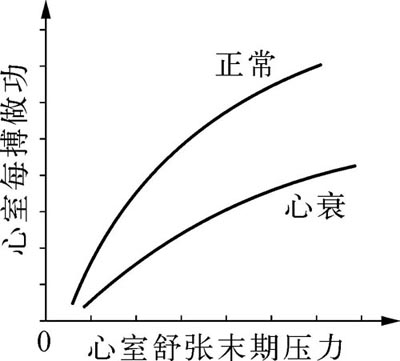
\includegraphics[width=5.91667in,height=3.03125in]{./images/Image00029.jpg}
\end{table}

实验室检查示:贫血、白细胞增多、血沉加快、类风湿因子低度阳性。血清中胞浆型抗中性粒细胞胞浆抗体(c-ANCA)阳性是诊断Wegener肉芽肿的重要参考指标。特异性为86\%,敏感性为78\%。

组织病理:鼻窦及鼻病变组织活检示坏死性肉芽肿及(或)血管炎。肾活检示局灶性节段坏死性肾小球肾炎。皮肤活检示白细胞破碎性血管炎。对临床表现有上、下呼吸道病变与肾小球肾炎者,实验室检查c-ANCA阳性,组织病理检查呈坏死性肉芽肿者可确诊。

此病与结节性多动脉炎的区别在于后者早期即出现肾脏损害,心脏通常明显受累。肺部症状主要为哮喘兼有嗜酸性粒细胞浸润和血中嗜酸性粒细胞增多等。此外还须与恶性中线性肉芽肿、特殊性传染性肉芽肿(结核性、梅毒性、真菌性等)、结节病、败血症、原发性肺癌等相鉴别。诊断主要依靠病理组织活检。

\subsubsection{五、混合性结缔组织病(MCTD)}

MCTD的特点为具有系统性红斑狼疮(SLE)、多发性肌炎、进行性系统性硬化、类风湿关节炎等多种结缔组织病的症状,肾脏损害轻。发热几乎经常出现。实验室检查显示高阳性率(达100\%)和高滴度的核糖核蛋白(RNP)抗体;荧光抗核抗体(FANA)达100\%阳性;而抗Sm抗体阴性,抗双链去氧核糖核酸抗体(ds-DNA)与狼疮细胞均呈低阳性率,C3、CH50均正常,提示MCTD是一种有特色的未分化结缔组织病。

\subsubsection{六、IgG4相关的硬化性疾病}

IgG4相关硬化性疾病是新近认识的一种疾病,是以累及胰腺以及胰腺外的肺间质,腮腺、泪腺、下颌腺等外分泌腺,胆道、后腹膜、肾脏、胃肠道、肝脏、乳腺等器官和脏器的慢性炎症性病变,血清学显示高γ球蛋白血症。病变部位以浆细胞浸润和纤维化为突出表现,可以检测到大量表达IgG4阳性的浆细胞,与自身免疫有关,且对类固醇激素治疗有效的一组异质性疾病。

患者可有不明原因发热、乏力、体重下降等全身表现,其他症状与受累器官组织有关,不同的器官组织受累有不同的表现,主要表现为局部压迫症状和相应腺体功能障碍。本病主要累及外分泌腺,多数患者胰腺受累,可表现为慢性轻中度腹痛、糖尿病。患者常因无痛性黄疸就诊,黄疸可呈波动性。涎腺、泪腺受累可出现腺体无痛性肿大,口眼干燥。此外,腹膜后纤维化的患者可出现腰背痛,因输尿管受压可能出现肾功能不全的表现。还有小管间质性肾炎、间质性肺炎、前列腺炎、乳腺炎等,症状均不特异。还可累及内分泌腺,包括垂体炎、Riedel甲状腺炎等。中枢神经系统受累很少见,但有硬脑膜、室管膜炎性假瘤和硬脑脊膜炎的报道。

多数患者出现高γ球蛋白血症,血清IgG、IgG4升高,IgG4/IgG比值升高,血清IgG4>1350mg/L对诊断AIP敏感性和特异性均很高,对诊断为AIP的患者,血清IgG>2200mg/L常提示胰腺外损害。

影像改变:累及胰腺时表现为胰腺弥漫性肿大,呈“腊肠样”,动态CT显示延迟强化。胰腺局灶性增大。内镜逆行胰胆管造影(ERCP)主胰管不规则狭窄,硬化性胆管炎患者胆管狭窄。肺部受累的CT表现主要分4型:实性结节型、圆形磨玻璃影型、肺泡间质型、支气管血管型。本病的肾损害主要在肾皮质,CT增强时表现为外围皮质圆形、楔形边界清楚的低密度影。

病理学组织淋巴浆细胞浸润、弥漫而致密的纤维化是这类疾病的特点;免疫组化显示,浸润的淋巴细胞主要是CD4\textsuperscript{+}
或CD8\textsuperscript{+} T细胞和IgG4\textsuperscript{+}
浆细胞,后者常超过30个/高倍镜。诊断依靠临床表现、血清学检查、影像学改变和病理学改变。

有报道一女性,56岁。不明原因发热3个月,腰痛1个月入院。胸部增强CT:后纵隔降主动脉周围软组织肿块,所示胸主动脉下段及腹主动脉旁不规则软组织影,包绕主动脉生长,下段腹主动脉旁及左侧髂总动脉旁不规则软组织影,包绕动脉生长,IgG
19.72g/L,IgG4:0.84g/L,行腹主动脉旁软组织活检术,病理:送检组织为大量增生纤维组织及脂肪和淋巴结一枚,淋巴结未见特殊病变,增生纤维组织中可见到大量浆细胞及中等量淋巴细胞,浆细胞浸润血管周隙及神经纤维束周围,酶标结果提示浸润淋巴细胞为CD4\textsuperscript{+}
T细胞,浆细胞分泌IgG为主,其中lgG4\textsuperscript{+}
细胞>20个/高倍视野,考虑IgG4相关硬化性疾病。

\protect\hypertarget{text00036.html}{}{}

\subsection{5.4 恶性肿瘤}

肿瘤性发热仅次于感染。恶性肿瘤患者长期发热见于两种情况:恶性肿瘤本身引起的发热和恶性肿瘤伴发感染所引起的发热。本处重点叙述肿瘤本身引起的发热。肿瘤热是由肿瘤细胞本身产生内源性致热因子,肿瘤迅速生长,瘤组织相对缺血、缺氧、坏死、出血引起吸收热;瘤组织坏死释放肿瘤坏死因子(TNF),TNF能诱导IL-1、IL-6的产生。TNF、IL-1、IL-6均为内源性致热原,而引起发热。

引起长期不明原因发热常见恶性实体瘤有原发性或继发性肝癌、肺癌、肾癌、甲状腺转移癌。较少见引起发热的有:结肠、卵巢、前列腺、乳腺、直肠、胰腺(无转移)和大脑恶性肿瘤、胃印戒细胞癌、松果体瘤、黑色素瘤、转移癌等。罕见引起发热的有嗜铬细胞瘤。此外,心房黏液瘤和胃、肾血管平滑肌脂肪瘤、小肠平滑肌瘤等是引起发热的良性肿瘤。

临床上,大多数恶性肿瘤引起的长期发热不超过38.9℃,如果超过此水平,一般提示感染性因素所致。热型多为弛张型或不规则型,患者通常无寒战,萘普生(naproxen)对肿瘤热有选择性解热作用。提示恶性肿瘤的其他症状是进行性消瘦、贫血等。对原因未明的低血糖状态、类白血病反应、游走性血栓性静脉炎、皮肌炎、纤维蛋白原缺乏症、红细胞增多症等情况,也须警惕恶性肿瘤的可能性;肾癌、肝癌、转移性肺癌、前列腺癌等,均可伴有红细胞增多症。癌也较常伴发于肺性肥大性骨关节病、皮肌炎、黑棘皮病等疾病。

肝癌:一些不典型或特殊表现的肝癌易被临床所忽视。肝大不明显,质不硬,甲胎蛋白反相间接血凝法或火箭电泳阴性,B超和CT有可能帮助发现本病,肝穿可找到确诊依据。

肾细胞癌很隐匿,约10\%的肾癌患者以发热为主要表现,通常仅表现为发热,无其他表现,有时伴乏力和消瘦,镜下血尿或血红细胞增多、血清碱性磷酸酶增高,可提示本病。B超、CT、选择性肾动脉造影有助于诊断。

嗜铬细胞瘤FUO,常见于发作性高血压病例,血压升高时体温增高,血压正常时体温降至正常。

肺癌通常不引起FUO,但部分病例在没有肺炎和肺不张的条件下表现为FUO。

心房黏液瘤可表现为发热、心脏杂音可呈现间隙性、体位性或缺如。血沉增快和贫血常见,超声心动图可确诊。

骨肉瘤也较常有发热的倾向。

\protect\hypertarget{text00037.html}{}{}

\subsection{5.5 中枢性发热}

下丘脑(间脑)综合征可由于炎症、肿瘤、外伤等引起,可导致长期不规则间歇发热,各项检查无急性感染的证据,血、尿培养均阴性,毒血症症状也不明显,应用各种抗生素而发热不能缓解。患者常伴有思睡、厌食或多食、肥胖、尿崩症、性功能减退以及自主神经功能紊乱症状等。

\protect\hypertarget{text00038.html}{}{}

\section{6 慢性低热}

体温上升达37.4~38℃(舌下测温)并除外生理性原因者称为低热;低热持续1个月以上者称为慢性低热。

有些高温作业的人、孕妇或女性排卵期,体温可较正常略高,但如离开高温环境或分娩后或排卵后,体温恢复正常,这种情况可称为生理性高体温,而非低热状态。

慢性低热可见于许多情况,一般可区分为器质性与功能性两大类(表\ref{tab2-23}),其中以器质性为常见;病因又以感染为多(表\ref{tab2-24})。

慢性低热的检查须注意下列情况:

\subsection{1.病史}

结核病史或结核患者接触史、咯血史、肝病史或黄疸史、局灶感染史、高温作业史等。

\subsection{2.体格检查}

需做全面体格检查,特别注意中耳炎、乳突炎、鼻窦炎、扁桃体炎、龋齿及齿根尖脓肿、前列腺炎等局灶性感染,贫血外貌,淋巴结与肝脾大,腹部压痛与包块,肾区叩击痛与压痛,脊柱压痛与纵轴叩击痛等。女性患者须考虑妇科检查。

\subsection{3.化验检查}

应作血、尿、便三项常规检查和血沉测定。未能除外感染或结缔组织病时,做抗链球菌溶血素“O”滴度测定、血清蛋白电泳测定、血中狼疮细胞检查,以及有关的血清免疫学检查。怀疑肝脏疾病时做常规肝功能试验。结核菌素试验强阳性有助于活动性结核病的诊断,但阴性未能排除此病。患者有未能解释的贫血时,须做骨髓象检查。

\begin{table}[htbp]
\centering
\caption{慢性低热疾病分类}
\label{tab2-23}
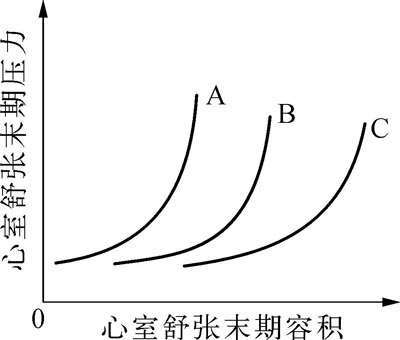
\includegraphics[width=5.875in,height=2.08333in]{./images/Image00030.jpg}
\end{table}

\begin{table}[htbp]
\centering
\caption{800例低热的原因分析}
\label{tab2-24}
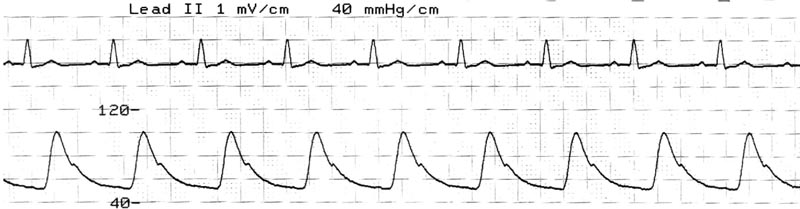
\includegraphics[width=6.03125in,height=6.08333in]{./images/Image00031.jpg}
\end{table}

\subsection{4.器械检查}

X线胸部透视应作为常规检查,需要时摄片。心电图描记、甲状腺吸131碘试验、超声肝区检查、胃肠钡餐透视与钡剂灌肠、眼底检查等,可按需要选择行之。未除外胆道感染者,有指征作十二指肠引流及(或)胆囊造影检查。疑为胸腹占位性变时做B超与CT检查。

\protect\hypertarget{text00039.html}{}{}

\subsection{6.1 器质性慢性低热}

\subsubsection{6.1.1 感染性慢性低热疾病}

\paragraph{一、结核病}

患者有慢性低热与结核中毒症状时,首先应考虑结核病。最常见的是肺结核,但早期可无呼吸系统症状与体征,X线透视检查也不一定完全可靠。有怀疑时应做胸部照片检查。

诊断困难者为肺外结核。肺外结核种类繁多,包括多系统、多脏器、多部位、多种类型的结核性病变。诊断比肺结核明显困难。为了避免误诊或漏诊,须注意:①进行全面、细致地病史询问和体检;②深部结核病灶或隐性病灶须选择X线、B超、CT、纤维内镜,甚至开腹探查协助诊断,从病理活检中确定诊断;③结核菌素试验;④如未排除隐性病灶的存在应采取积极的有效抗结核诊断性治疗,疗程不少于4~6周。由于近年来结核病有复燃之势,诊断性治疗临床症状奏效之后,对疑似病例仍需继续正规治疗,不能半途而废。

诊断上较难的肺外结核病变,如肾结核大多数发生于20~40岁之间,主要症状不表现于肾而表现于膀胱,约75\%~85\%患者有膀胱刺激征,如尿频、尿急与尿痛。主要化验所见为血尿,多为镜下血尿,有时为肉眼血尿,常间歇出现。其他症状为低热、腰痛、纳差、盗汗、消瘦、倦怠等。

肝结核少见,也可引起慢性低热,结核菌素试验阴性不能除外此病,临床上不易诊断。CT扫描有助于发现粟粒病灶。

骨结核主要侵犯儿童与年轻成人。骨结核好发于脊椎,最常侵犯腰椎或胸椎,易于漏诊,腰背部局限性隐痛及(或)固定性局限性脊椎压痛提示此病的诊断。

肠系膜淋巴结结核,主要侵犯儿童与青少年,常与肠结核及结核性腹膜炎并发。凡年轻患者有原因未明的慢性发热与结核中毒症状、血沉加快、营养不良及与饮食无关的腹痛,即使腹部未触及包块,也须考虑腹腔内淋巴结结核的可能性,结核菌素试验强阳性(但阴性未能除外本病)和腹部X线摄片发现钙化灶,有力地支持本病。抗结核药物诊断性治疗奏效时可证实临床诊断。本病往往须手术探查方能明确诊断。

女性生殖器结核,主要侵犯附属器官,症状不典型,临床诊断不易。发病多在20~40岁之间,往往有低热、倦怠、下腹痛、盗汗、体重减轻等症状。妇科病征则有月经稀少,闭经与不育。遇见女性结核患者,尤其是肺结核病或腹膜结核,或患者有全身性结核病症状而找不到病灶,而同时有不育症,月经稀少或闭经,应考虑女性生殖器结核的可能性。

肾上腺结核少见,此病临床上往往表现为Addison病。国内一组3例原发病为肺结核,肾上腺结核均经CT证实。

\paragraph{二、慢性非特异性局灶性感染}

扁桃体、齿根、鼻窦、中耳、乳突、胆道、肠道、肾盂、前列腺、女性内生殖器等处的慢性炎症,也有引起慢性低热的可能,但以不规则的波动性发热为多见。患者除局部病征之外,并常有精神体力欠佳、血沉轻度加快等表现。有的患者伴有心悸、多汗、皮肤划痕症等自主神经功能紊乱症状。局灶性感染根治后,低热及其他症状也随之消退。

链球菌感染后状态:临床上可见到一些扁桃体炎或咽炎之后出现低热、关节酸痛。心率加快、抗“O”增高,血沉正常或轻度加快,咽拭子培养可证明乙型溶血性链球菌,心电图检查可发现短暂的期前收缩或(及)轻度S-T段与T波改变。无心脏增大与心杂音。给予青霉素或其他抗菌药物治疗,常于短期内解热。关节痛及其他症状均消失;如病情改善不明显,加用小剂量泼尼松也奏效。这种情况可称为链球菌感染后状态,如经上述治疗病情仍无好转或有再发,须考虑为风湿热或其他并存的疾病。

\paragraph{三、慢性病毒性肝炎}

慢性无黄疸型病毒性肝炎可引起低热。患者除有食欲减退、肝区隐痛、肝大压痛等肝炎表现外,常兼有多汗、易兴奋、失眠等自主神经功能紊乱症状。低热于休息时较低,活动或劳累略有升高,热程可累月甚至经年。患者肝功能多有异常,还可在血清中检出特异性肝炎标志物。十二指肠引流有时可发现“B”、“C”管的胆汁中白细胞数增加,容易与胆道感染相混淆。胆汁培养无细菌生长,镜检无寄生虫发现,诊断性治疗不奏效,据此可与慢性胆道感染相区别。

\paragraph{四、巨细胞病毒感染}

近年有人注意到巨细胞病毒感染所致的持续微热状态。这种病毒感染又称为全身性巨细胞性包涵体病,其临床表现变异很大。可表现为类似传染性单核细胞增多症的综合征,但嗜异性凝集反应阴性。也可引起慢性肝脏病变。表现为慢性无黄疸型肝炎。诊断须依靠血、尿的病毒分离培养,巨细胞病毒补体结合试验,尿路上皮细胞中发现细胞核内包涵体等。

\paragraph{五、梅 毒}

梅毒第二期以后的表现较为复杂。如患者有梅毒接触史,血清梅毒抗体特异性试验阳性,而有原因未明的慢性低热,应考虑此病的可能性。

\paragraph{六、艾滋病}

艾滋病亦可表现为慢性低热。

\paragraph{七、其 他}

也见有个案报道布鲁杆菌病、伤寒、POEMS、恶性间叶瘤也可引起低热。

\protect\hypertarget{text00040.html}{}{}

\subsubsection{6.1.2 非感染性慢性低热疾病}

\paragraph{一、甲状腺疾病}

甲状腺功能亢进、甲亢危象,亚急性甲状腺炎、甲状腺癌中滤泡细胞型者、少数桥本病表现为亚急性甲状腺炎或甲亢,均可有不同程度发热和出汗,这些患者发热同时多有高代谢症候群。

\paragraph{二、风湿性疾病}

风湿性疾病以发热为主要临床表现,因此呈慢性低热者亦有之。这种情况可见于风湿热、系统性红斑狼疮、结节性多动脉炎、皮肌炎,结节病、大动脉炎、小血管炎也见有个案报道表现为低热。

\paragraph{三、肝硬化}

肝硬化患者约1/4~1/3有发热,大多由于肝细胞坏死或肝内炎症等活动性病变所致。部分病例呈低热,常未能发现任何发热的原因。发热较高时往往提示合并感染。

\paragraph{四、炎症性肠病}

Crohn病及溃疡性结肠炎,均可有慢性低热,提示轻度的炎症活动。

\paragraph{五、失代偿性心瓣膜病}

失代偿性心瓣膜病可能有持续的低热,由于淤血性支气管炎、细小的肺梗塞或血栓性静脉炎等所致。或认为在充血性心力衰竭时,由于心排血量降低、皮肤血流量减少以及水肿的隔热作用,使散热减少,再由于呼吸困难时呼吸肌运动量增加,使热的产生有所增加,故可有低热。

如患者持续低热兼有关节(肿)痛,心律失常如心房颤动、阵发性心动过速、期前收缩的出现,洋地黄耐受量降低,新的瓣膜病变杂音的出现或心杂音的改变(包括强度增加与音质改变)等情况,则应考虑活动性风湿性心脏病。如持续低热兼有栓塞现象(皮肤或结膜瘀点),则提示并发亚急性细菌性心内膜炎的可能性。

\paragraph{六、血液病}

重症贫血患者常有低热,乃由于基础代谢率稍有增高之故。慢性白血病与恶性淋巴瘤也可有低热。少见病Castleman病也可以长期低热。

有报道:男,34岁,反复午后低热11年,37.2~37.5℃,浅表淋巴结肿大,最大直径2cm,病初淋巴结活检示淋巴结反应性增生,短期糖皮质激素治疗淋巴结有缩小,但仍反复低热,11年后除了浅表淋巴结肿大外、肝脾大,白细胞低、小细胞低色素性贫血;高球蛋白血症,多克隆性免疫球蛋白及轻链升高;PT、APTT延长,反应性浆细胞增多。低氧血症,双肺弥漫性病变,蛋白尿,镜下血尿,B超示双肾弥慢性病,淋巴结活检示Castleman病。

\paragraph{七、恶性肿瘤}

恶性肿瘤有发热的倾向,特别是肺癌、肝癌、结肠直肠癌。低热一般见于无并发症和无进行性急剧坏死的恶性肿瘤。中年以上患者有慢性低热与血沉加快,虽无任何其他病征,也须注意深部恶性肿瘤的可能性。

\paragraph{八、间脑(下丘脑)综合征}

间脑由丘脑、丘脑底、下丘脑和第三脑室周围结构所组成,是大脑皮质和各低级部位相互联系的重要机构。间脑综合征较下丘脑综合征有更广的范围,二者都可引起体温调节障碍,以及一系列自主神经失调症状,症状还有发作性的特点。

下视丘视前区两侧急性病变常引起体温迅速升高;慢性起病的间脑综合征则不少有低热。发病以21~40岁为多。据我院1963年总结30例的经验,病因以感染为多,其次为脑外伤、肿瘤、中毒等,但也有原因未明者。

间脑功能十分复杂,间脑病损主要有下列表现:

\subparagraph{1.自主神经功能紊乱症状}

如多汗或无汗;多尿或少尿,脉快或脉慢,血压升高或降低,发作性头昏,皮肤划痕症等。此外尚可表现为半侧感觉障碍、半侧水肿。半侧皮肤发红、半侧无汗或多汗等。

\subparagraph{2.内分泌代谢障碍}

如肥胖,糖耐量曲线异常,剧烈饥饿感、皮肤不对称性水肿,性欲减退,月经不正常,不育等。

\subparagraph{3.睡眠障碍}

如嗜睡或失眠,倒错性睡眠(白天嗜睡,夜间不睡)。

\subparagraph{4.体温调节障碍}

以慢性低热最为多见。低热的特点是:①对解热药呈异常反应;非间脑病变时,服阿司匹林后开始时皮肤温度升高,而在间脑病变时呈倒错反应(即开始时皮温下降)或无反应。②两半侧身体皮肤温度不对称现象,在间脑病变时相差甚明显,如相差在0.4~
0.5℃时可认为是病理性。③24小时体温曲线正常人在下午较高,连续测量数天在间脑病变有时上午较高。

间脑综合征的诊断主要根据:①有关的既往病史;②在短期内出现上述大部分症状;③症状分布为全身性或半侧性;④有发作性的特点;⑤脑电图各导联阵发性出现θ波有助于诊断。其病因的诊断较难,必须联系下丘脑的生理功能,结合有关下丘脑靶腺反馈机制,头颅CT和磁共振等影像学特征作出诊断。

\paragraph{九、更年期症候群}

更年期症状与体征均与雌激素水平下降有关,常见症状为阵发性潮红,尤其面颈部皮肤多见,可持续数年,其次为发热和出汗,也多有阵发性规律,感觉异常,手脚发凉,头晕头痛、失眠,健忘,精力不集中,精神紧张,焦虑,神经质等更为多见,血浆雌二醇及孕酮降低,促卵刺激素升高,促黄体生成素多正常,结合年龄和闭经史诊断较易。

\protect\hypertarget{text00041.html}{}{}

\subsection{6.2 功能性低热}

功能性低热的临床特征是患者体温较正常人升高约0.3~0.5℃左右,一般不超过38℃。经反复体检,病理学和实验室检查,除体温升高外未见其他异常,长期观察,一般情况良好,不影响正常工作和生活,经抗感染、抗结核、抗风湿等治疗无效。

\subsubsection{一、感染后低热}

在其前往往有细菌、病毒、衣原体、原虫等感染,特别多见于病毒感染后。此时体温调节中枢对体温的调节功能仍未恢复正常所致。

\subsubsection{二、手术后低热}

手术后可以有术后吸收热,一般在术后6~8小时开始发热,持续3~5天可自行缓解,但部分患者低热持续,而与手术相关的切口等均正常。

\subsubsection{三、功能性低热}

多见于青年女性,为一种原发性低热,日间温差不大(相差0.5℃左右),体温昼夜规律失常。晨间午前往往较下午晚间略高,体力活动体温可不升或有时反而下降。持续数月、数年,体温往往在偶然或患者不注意情况下自动下降。患者又常兼有多汗、手颤、皮肤划痕症、呼吸性不整脉、怕冷、心悸、失眠等自主神经功能紊乱的表现。

\subsubsection{四、夏季低热}

低热仅发生于夏季,秋凉后自行退热,每年如此反复出现,连续数年后多可自愈。多见于幼儿,因体温调节功能不完善,夏季身体虚弱,且多发生于营养不良或脑发育不全者。

\subsubsection{五、其 他}

妊娠初期也可有低热现象。部分妇女月经前7~10天体温上升至37.5℃,月经来潮后体温降至正常。

功能性低热的诊断需根据较长时间的观察,排除各种器质性疾病,如肺外结核、甲亢、恶性肿瘤,在女性尤需注意卵巢癌,男性患者诊断功能性低热需慎重。

\protect\hypertarget{text00042.html}{}{}

\section{参考文献}

1.胥婕,等.北京地区250例严重急性呼吸综合征患者临床分析.中华结核和呼吸杂志,2003,26(11):683-685

2.倪安平.衣原体的肺部感染.中华结核和呼吸杂志,1998,21(9):516-517

3.李丽,等.鹦鹉热衣原体肺炎一例.中华结核和呼吸杂志,1999,22(11):662

4.刘忠达,等.恙虫病肺部合并症50例临床分析.中华结核和呼吸杂志,2002,25(8):478-480.

5.陈晓红.恙虫病致肺损害46例.中华传染病杂志,2002,20(5):312-313

6.张溪林,等.恙虫病致急性肺损伤/急性呼吸窘迫综合征.中华传染病杂志,2003,21(6):436-437

7.黄学焕,等.96例肺下叶结核的诊断与鉴别诊断.中华内科杂志,1994,33(8):515

8.梁思礼,等.类鼻疽肺病四例报告与文献复习.中华结核和呼吸杂志,1994,17(3):168-170

9.陆慰萱,等.嗜肺军团杆菌肺炎37例综合分析.中华结核和呼吸杂志,1997,20(2):91-94

10.张斌,等.变态反应性支气管肺曲霉病.中华结核和呼吸杂志,1999,22(6):377-378

11.文仲光,等.肺毛霉病------附二例报告.中华内科杂志,1998,37(5):327-329

12.张可,等.艾滋病合并卡氏肺孢子虫肺炎的临床特点及诊断方法.中华结核和呼吸杂志,2002,25(8):475-477

13.金明根,等.生食鳖所致比翼线虫病的临床分析.中华结核和呼吸杂志,1998,21(10):611

14.燕航,等.肾移植术后巨细胞病毒肺炎的诊治.中华器官移植杂志,2001,22(5):298-300

15.徐志松,等.异基因骨髓移植后巨细胞病毒肺炎的临床研究.中华结核和呼吸杂志,2004,27(9):646-647

16.徐小元,等.人禽流感的流行病学与生物学.中华医学杂志,2004,84(5):353-354

17.林江涛.人禽流感的诊断治疗策略.中华医学杂志,2004,84(5):355-356

18.刘又宁,等.中国城市成人社区获得性肺炎665例病原学多中心调查.中华结核和呼吸杂志,2006,29:3-8

19.中华医学会呼吸病学分会感染学组.肺真菌病诊断和治疗专家共识.中华结核和呼吸杂志,2007,30:821-834

20.唐可京,等.肺接合菌的诊治.中华结核和呼吸杂志,2009,32:793-796

21.Gupta SK,et al.Evaluation of the Winthrop-University Hospital
criteria to identify Legionella pneumonia. Chest.2001,120(4):1064-71

22.Agarwal R,et al.Aspergillus hypersensitivity in patients with
chronic obstructive pulmonary disease:COPD as a risk factor for
ABPA?Med Mycol.2010,48:988-994

23.中华人民共和国国家卫生和计划生育委员会.人感染H7N9禽流感诊疗方案(2013年第2版).中华临床感染病杂志,2013,6(2):65-67

24.韩明锋,等.国内102例人感染H7N9禽流感特点初步分析.传染病信息,2013,26(2):68-70

25.权菊香,等.2013年我国H7N9型禽病毒流感分析.中国临床药理学杂志,2013,29(6):426-428

26.杨钧,等.甲型H1N1流感合并肺炎的影像表现.中华放射学杂志,2010,44(2):119-122

27.陈枫,等.重症及危重症甲型H1N1流感肺炎的影像表现.中华放射学杂志,2010,44(2):123-126

28.罗宏,等.新型甲型H1N1流感重症患者肺部影像学变化及临床特点.中华结核和呼吸杂志,2010,33(6):415-418

29.Fujitani S,et al.Pneumonia due to Pseudomonas
aeruginosa:partⅠ:epidemiology,clinical diagnosis,and
source.Chest,2011,139(4):909-919

30.廖纪萍,等.军团菌肺炎的临床诊治进展.国际呼吸杂志,2007,27(21):1632-1636

31.姚郁林,等.肺出血型钩端螺旋体病113例X线诊断体会.山东医药,2008,48(25):47

32.刘又宁,等.中国1998年至2007年临床确诊的肺真菌病患者的多中心回顾性调查.中华结核和呼吸杂志,2011,34(2):86-90

33.姚婉贞.侵袭性肺曲霉病的诊断与治疗.中华结核和呼吸杂志,2011,30(11):812-814

34.何礼贤,等.慢性阻塞性肺疾病合并侵袭性肺曲霉病的病理生理特点及其诊断策略.中国真菌学杂志,2011,6(5):257-260

35.何礼贤.肺孢子菌肺炎的诊断与治疗.中华结核和呼吸杂志,2007,30(11):802-805

36.张波.急性间质性肺炎的诊断与治疗.上海医学,2009,32(10):843-844

37.庄谊.隐源性和继发性机化性肺炎临床和影像学特点分析.实用临床医药杂志,2011,15(19):147-149

38.降钙素原急诊临床应用专家共识组.降钙素原急诊临床应用的专家共识.中华急诊医学杂志,2012,21
(9):944-951

39.蔡闯,等.2009年甲型H1N1流感研究近况.中国急救医学,2009,29(6):553-555

40.权菊香,等.2013年我国H7N9型禽病毒流感分析.中国临床药理学杂志,2013,29(6):426-428

41.谢正德.儿童EB病毒传染性单核细胞增多症临床特征及诊断标准.实用儿科临床杂志,2007,22(22):1759-1760

42.林特夫,等.细菌L型感染的意义和研究进展.蚌埠医学院学报,2006,31(2):111-115

43.童强,等.肾移植术后巨细胞病毒性肺炎的诊断与治疗.解放军医学杂志,2006,31(7):716-771

44.倪莲芳,等.组织细胞坏死性淋巴结炎68例临床分析.中华医学杂志,2010,90:3147-3149

45.谭明旗,等.组织细胞性坏死性淋巴结炎48例临床分析.中国实用内科杂志,2003,23(1):51

46.刘本似,等.我国西藏地区兔热病(土拉菌病)14例报告.流行病防治研究,1974,(3):224

47.何远学.钩端螺旋体病26例临床分析.中国热带医学,2006,6(10):1830

48.林瑞炮,等.凶险型恶性疟疾临床分型及治疗.中华传染病杂志,2002,20(5):317

49.郑德福,等.1964-2011年中国大陆人体旋毛虫病流行分析.寄生虫病与感染性疾病,2011,9(3):119

50.李兴福,等.急性风湿热诊断的相关问题.临床内科杂志,2005,22(10):652

51.赵丹,等.登革热预警技术研究进展.中华流行病学杂志,2012,33(5):540

52.张顺先,等.我国2005~2012年登革热流行特征分析.中国医药指南,2013,11(16):401

53.罗雷,等.广州市1978至2006年登革热流行病学特征分析.中华传染病杂志,2008,26(8):490

54.查震球,等.175例恙虫病病例的临床和流行病学特征研究.中华疾病控制杂志,2010,14(8):720

55.张萌,等.中国恙虫病流行态势及预防控制.中华流行病学杂志,2011,32(4):419

56.杨晴,等.恙虫病临床特点分析.中华实验和临床感染病杂志(电子版),2011,5(1):42

57.胡相,等.一起人的类丹毒流行病学调查.中华预防医学杂志,1980,14(4):213

58.黄奕江.类鼻疽病的诊断与治疗.临床内科杂志,2010,27(8):512

59.林容,等.类鼻疽病122例临床特征及耐药性分析.广东医学,2011,32(17):2303-2304

60.杨柳,等.Lyme病的临床分析及诊断探讨.中国实用眼科杂志,2000,18(11):712

61.张清安,等.皮肌炎与多发性肌炎73例临床分析.中国实用内科杂志,2005,25(4):354

62.曾泉.变应性血管炎82例临床分析.中国医药指南,2013,11(16):238

63.虞瑞尧.发疹性传染病与药疹的诊断、鉴别诊断与治疗.传染病信息,2007,20(1):23

64.王红兵,等.成人变应性亚败血症8例临床分析.中国麻风皮肤病杂志,2006,22(2):173

65.马科,等.不明原因发热15年临床变迁.中华医院感染学杂志,2008,18(9):1279

66.陈志海,等.北京地区肾综出血热96例临床特征分析.中华内科杂志,2003,42(1):70

67.娄秀芬,等.感染性心内膜炎120例临床分析.中华内科杂志,2009,48(1):35-38

68.谢旭晶,等.近十年风湿热的演变.中华风湿病学杂志,2009,13(7):467

69.刘正印,等.药物热40例临床分析.中国实用内科杂志,2000,20(6):364-365

70.孟卉秦,等.麻疹145例临床分析.中国实用内科杂志,2002,22(5):300-301

71.王南,等.风疹118例流行特点及临床分析.中国实用内科杂志,2003(23):754

72.张小河.恙虫病诊治探讨.医药论坛杂志,2009,30(5):27

73.韩秀萍,等.皮肌炎、多发性肌炎52例临床分析.中国实用内科杂志,2004(24):430

74.陈林囡,等.成人斯蒂病的临床表现和治疗探讨.中国风湿病学杂志,2002,6(6):173-174

75.阮力,等.特殊首发表现的急性白血病20例误诊分析.中国实用内科杂志,2004,24(6):374-376

76.唐井钢,等.98例不明原因长期发热病因分析.中国现代医学杂志,2008,15:2258-2259

77.陈珺秋.系统性红斑狼疮38例临床分析.中外医学研究,2012,30:141-142

78.左晓霞.结缔组织病与发热.中国感染控制杂志,2009,05:297-300

79.中华医学会风湿病学分会.结节性多动脉炎.中华风湿病学杂志,2004,8(7):436-437

80.段新旺,等.韦格纳肉芽肿病34例临床分析.中华急诊医学杂志,2012,21(10):1159-1163

81.张国华,等.韦格纳肉芽肿病100例临床分析.中华风湿病学杂志,2010,14(10):677-681

82.中华医学会风湿病学分会.韦格纳肉芽肿病诊断和治疗指南.中华风湿病学杂志,2011,15(3):194-196

83.林果为.提高对长期发热为主要表现恶性淋巴瘤的诊断水平.上海医学,2002,25(3):133

84.姚秋菊,等.不明原因发热103例病因分析.中华传染病杂志,2003,21(6):427

85.韩红,等.成人不明原因发热急诊的临床研究.中华急诊医学杂志,2010,19(6):647-649

86.马小军,等.不明原因发热449例临床分析.中华内科杂志,2004,43(9):682-685

87.林昌锋,等.原因不明发热者122例分析.中国误诊学杂志,2011,35:8707-8708

88.江红,等.原因不明发热患者128例临床分析.中华传染病杂志,2007,10:621-623

89.侍效春,等.综合医院以不明原因发热为表现的结核病100例临床分析,中华内科杂志,2010,49(12),1002-1004

90.马科,等.不明原因发热15年临床变迁.中华医院感染学杂志,2008,18(9):1279-1281

91.楼国春,等.钩虫病致周期性发热一例.中华内科杂志,2004,43(8):632

92.牟向东,等.肺黏膜相关淋巴组织型边缘区B细胞淋巴瘤一例.北京大学学报(医学版),2007,39(4):346-350

93.王孝勤.回归热误诊一例.临床误诊误治,2004,17(1):72

94.喻艳林,等.10例人粒细胞无形体病暴发流行报告.中华传染病杂志,2010,28(3):168-170

95.谭阳,等.周期性发热综合征.中国实用儿科杂志,2004,19(1):51-54

96.雷玲田,等.脂膜炎患者的临床特征及治疗随访分析.中华风湿病学杂志,2009,13(1):36-38

97.李龙芸,等.124例疑难发热病的诊断.中华内科杂志,2000,39(5):323

98.朴雪梅,等.IgG4相关的硬化性疾病一例.中华风湿病学杂志,2010,14(11):790-791

99.黄晓燕,等.IgG4相关硬化性疾病.中华内科杂志,2010,49(10):891-893

100.罗金梅,等.第115例------全身淋巴结肿大、低热伴活动后气短.中华结核和呼吸杂志,2011,34(8):631-633

101.田瑛,等.以不明原因发热就诊的肿瘤患者42例临床分析.中华内科杂志,2010,41(11):727-728

102.翁心华,等.原因不明发热的病因诊断与合理治疗.中华内科杂志,2003,42(4):269-270

103.卢洪洲,等.原因不明发热142例病因分析.中华内科杂志,2005,44(6):466-468

104.Henter JI,et al.HLH-2004:Diagnostic and therapeutic guidelines for
hemophagocytic lymphohistiocytosis.Pediatr B1ood
Cancer.2007,48:124-131

105.李剑,等.不明原因发热为首发表现的淋巴瘤53例临床分析.中华内科杂志,2006,45(8):665-667

106.北京朝阳医院内科.800例低热患者临床分析.中华医学杂志,1975,55:331

\protect\hypertarget{text00043.html}{}{}


\chapter{呼吸困难}

呼吸困难是指患者主观上有空气不足或呼吸费力的感觉,而客观上表现为呼吸频率、深度(如呼吸速而浅或慢而深)和节律的改变。患者用力呼吸,可见辅助呼吸肌参与呼吸运动,严重者可呈端坐呼吸及发绀。

根据主要的发病机制,可将呼吸困难区分为下列五种基本类型。能引起呼吸困难的疾病繁多,见表\ref{tab3-1}。

\begin{table}[htbp]
\centering
\caption{呼吸困难疾病的分类}
\label{tab3-1}
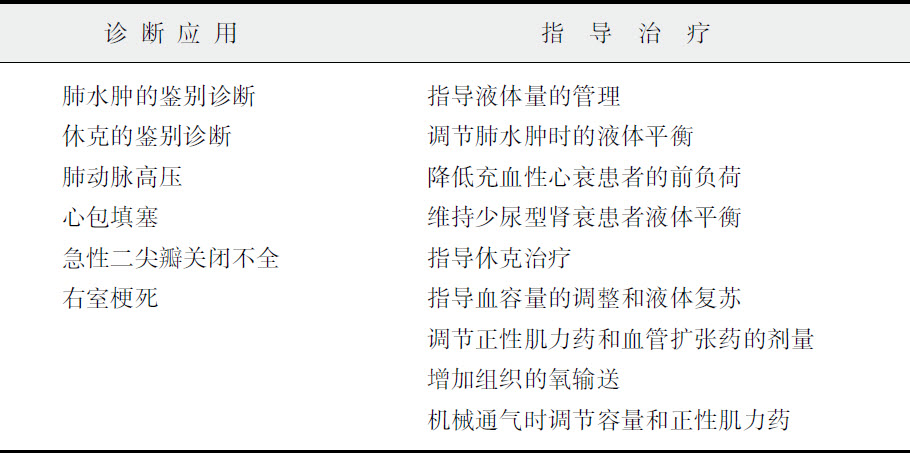
\includegraphics[width=5.95833in,height=5in]{./images/Image00032.jpg}
\end{table}

根据呼吸困难发生的缓急和伴随症状,可对呼吸困难作出初步的鉴别诊断:

\section{【急性发生的呼吸困难】}

1.时间超过1~2小时,伴有喘息者 支气管哮喘(病史可参考)、左心功能衰竭(心肌梗死、瓣膜病等)。

2.时间超过数小时/数天,伴有发热,有痰或无痰者 肺炎、急性支气管炎、急性胸膜炎、急性化脓性纵隔炎、急性心包炎等疾病。

3.高通气伴有代谢性酸中毒者 须考虑肾衰竭、糖尿病酮症酸中毒;有中毒者多为水杨酸盐、甲醇等。高通气综合征多为无心肺疾病的年轻女性。

4.呼吸困难同时伴有胸痛者 多为气胸(有气管移位)、肺栓塞(多有下肢静脉血栓,可有休克)、大叶性肺炎、急性心肌梗死、急性心包炎、急性胸膜炎、气道异物等。

5.产妇破水后突然出现呼吸困难、发绀、休克,应考虑为肺羊水栓塞症。长骨骨折后发生呼吸困难,须考虑肺脂肪栓塞。胸、腹大手术后突发呼吸困难,须考虑胸腔积液或肺不张。

\section{【慢性发生的呼吸困难】}

1.伴有胸膜炎性胸痛应注意胸腔积液、叶性肺不张、气胸、肺炎和肺栓塞等。

2.伴有大量脓性痰者多为支气管扩张,小量脓性痰可见于慢性支气管炎、支气管哮喘和肺炎。大量粉红色泡沫痰则见于急性左心功能不全,但也可见于肺泡细胞癌。

3.伴有咯血者如胸部X线检查显示中央气道异常可能是肺癌,胸部X线检查正常则可能为肺栓塞或肺血管炎(如Goodpasture综合征、多发性动脉炎)。

4.伴有全身衰弱者应注意神经肌肉疾病,如重症肌无力和运动神经元疾病。

\section{【如何评价呼吸困难】}

\subsection{(一)病史}

心、肺、胃肠病及肾脏病史,以往气喘发作史及诊疗经过,内因性与外因性中毒,职业性粉尘或异物吸入史,过敏病史,用药史,高原居留史。

病史询问应了解下列问题:①呼吸困难是突然发生还是逐渐发生?②患者的年龄,以及症状缓解和恶化的特点?③是休息还是活动时出现呼吸困难?④出现呼吸困难症状时的活动程度如何?临床上常用改良的呼吸困难分级量表(modified
Medical Research Council dyspnoea
scale,mMRC)评估呼吸困难程度,特别适用于慢性支气管炎和慢性阻塞性肺疾病患者。mMRC分为0~4级共5个级别,级别越高,患者呼吸困难越重:其中0级表示患者仅在费力运动时出现呼吸困难;4级表示患者因严重呼吸困难不能离开家,或在脱/穿衣服时出现呼吸困难。急性呼吸困难常常导致严重的后果,需要立刻评估和治疗(表\ref{tab3-2})。

\begin{table}[htbp]
\centering
\caption{呼吸困难程度}
\label{tab3-2}
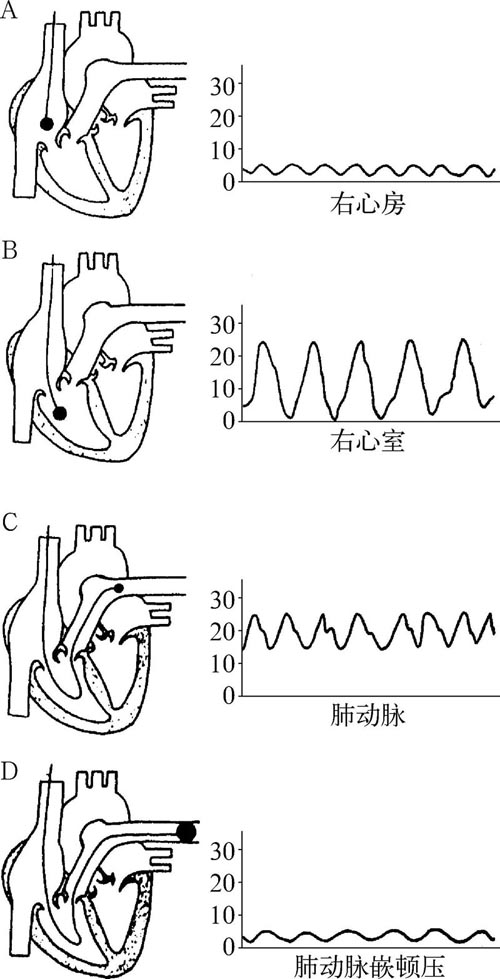
\includegraphics[width=5.90625in,height=1.39583in]{./images/Image00033.jpg}
\end{table}

\subsection{(二)体检}

咽、喉与胸部体征,肝脾大,腹水、水肿。肺部是体检的重点。另外还需评估患者的心脏情况,排除心脏疾病。

\subsection{(三)化验检查}

血象,嗜酸性粒细胞计数,有指征时作血尿素氮、血糖测定、动脉血气分析与酸碱度测定、痰检查(包括痰涂片找抗酸杆菌、痰培养和痰的细胞学分析等)。

\subsection{(四)器械检查}

X线胸部透视或(及)摄片;有指征时作静脉压测定、血循环时间测定、心电图描记、肺功能检查、放射性核素肺扫描、CT、纤维支气管镜检查、肺血管造影等。

\protect\hypertarget{text00044.html}{}{}

\section{7 肺源性呼吸困难}

广义的肺源性呼吸困难是由于呼吸器官(包括上呼吸道、支气管、肺、胸膜)病变、纵隔病变、胸廓运动以及呼吸肌功能障碍等所致,可分为下列三种表现形式:

\subsection{(一)吸气性呼吸困难}

可见于急性咽后壁脓肿、喉水肿、喉痉挛、喉及气管内异物、咽、喉白喉、喉癌、气管息肉、气管肿瘤、气管受压(气管周围脓肿、甲状腺肿瘤或甲状腺术后出血等)等疾病。由于喉、气管与大支气管狭窄与阻塞所致。

\subsection{(二)呼气性呼吸困难}

可见于急性细支气管炎、支气管哮喘、慢性阻塞性肺气肿、外源性过敏性肺泡炎等疾病。由于肺组织病变如弹性减弱及小支气管痉挛、狭窄所致。

\subsection{(三)混合性呼吸困难}

可见于慢性阻塞性肺气肿合并肺部感染,大量胸腔积液,自发性气胸,广泛性肺实质性病变如急性粟粒型肺结核,大叶性肺炎与支气管肺炎,大片肺不张以及急性肺水肿等疾病。由于肺呼吸面积减少所致。

\protect\hypertarget{text00045.html}{}{}

\subsection{7.1 上呼吸道疾病}

喉与气管病变所致的呼吸困难,其特点是吸气性呼吸困难,吸气时带有喘鸣音,常伴有声嘶与失音,呼吸深大但不快,吸气时呼吸肌运动加强,并可出现胸骨上窝、锁骨上窝与肋间的凹陷现象。

\subsubsection{一、咽后壁脓肿}

咽后壁脓肿多见于小儿,较少见于成人。年龄愈小或脓肿愈近喉部,则呼吸困难愈明显,并有喘鸣音、吞咽疼痛、吞咽困难。由咽后壁淋巴结化脓及异物损伤咽后壁所致的非特异性化脓性脓肿,其起病急骤,并有化脓感染的全身性症状;由结核菌引起的脓肿则呈慢性经过。

本病的诊断可根据:①咽部视诊可发现咽后壁红肿,轻触脓肿部位有波动感;②颈椎侧位X线摄片可显示咽后壁隆起的软组织肿胀;③结核性者可有颈椎结核的X线征。

\subsubsection{二、喉及气管内异物}

喉及气管内异物绝大多数发生于5岁以下的小儿及昏迷患者。异物卡住喉腔可引起高度呼吸困难以致窒息。异物进入气管内则引起刺激性咳嗽,以后停留在恰能容下其大小的部位,引起阻塞性肺气肿、肺不张与局灶性感染。异物多为食物、骨头、果核、小金属物和笔套等;在昏迷患者则为呕吐物、假牙等。胸部X线检查,可发现不透X线的异物影、局限性肺气肿、肺不张或阻塞性肺炎。喉镜或纤维支气管镜检查有助于观察异物的大小、性状与所在位置,并可在直视下取出异物。

\subsubsection{三、喉水肿}

喉水肿多急骤起病,水肿波及整个黏膜下层时,病情较轻者有喉内异物感、吞咽梗阻感、干咳、声嘶,严重者则引起呼吸困难。如声门或声门下区水肿,可迅速产生致命的喉梗阻。

引起喉水肿的原因可分为感染性和非感染性二类。感染性者,如化脓性咽喉炎、喉结核、喉部脓肿;非感染性者,如血管神经性水肿、药物过敏(如碘剂、乙酰水杨酸等)、喉部外伤、异物损伤及刺激(如气管插管)、高热蒸气或强烈化学气体(如氯气、光气、氨气、二氧化硫气等)刺激、腐蚀剂(如高浓度高锰酸钾溶液)刺激等。

血管神经性水肿所致的喉水肿,多有身体其他部位过敏征象出现,且有多次反复发作史;药物过敏性喉水肿有服用药物史;喉部化脓性炎症有明显感染症状。

\subsubsection{四、咽、喉白喉}

咽白喉约占白喉患者的80\%,病情轻者有咽痛、低中度发热,无明显全身中毒症状。重型和极重型患者有高热、头痛、面色苍白、呼吸急促、呼吸困难、烦躁不安、脉细速等全身中毒症状,并可出现中毒性心肌炎、周围神经麻痹,甚至中毒性休克。体检咽部充血,扁桃体肿大,咽部有点状或小片状灰白色假膜形成,不易剥离。有些患者咽部假膜范围广且厚,可呈污秽的黑灰色,有腐败口臭,扁桃体及咽部高度肿胀,可有坏死或溃疡,可合并其他细菌感染;颈部淋巴结肿大,周围软组织水肿,可蔓延至胸部,状似“牛颈”。

喉白喉约占白喉患者的20\%,多见于小儿,多数由咽白喉蔓延而来,起病略缓。白喉假膜和喉局部炎症、水肿引起气道狭窄,出现喉痛、吞咽困难、“犬吠”样咳嗽、声嘶、吸气性呼吸困难与喘鸣音,以及全身中毒症状,严重喉梗阻者吸气时出现“三凹征”。假膜涂拭物涂片染色或培养检查发现白喉杆菌而确诊。

喉白喉须与急性喉炎区别。小儿有发热、“犬吠”样咳嗽、声音嘶哑、吸气性呼吸困难者,应考虑喉白喉与急性喉炎。后者起病急骤、高热、呼吸困难常呈昼轻夜重,喉镜检查无灰白色假膜发现。

\subsubsection{五、急性会厌炎}

急性会厌炎又称急性声门上喉炎,好发于成人,可分两种临床类型,即渐进型(缓慢型)和速发型(暴发型)。咽部疼痛和吞咽困难是成人急性会厌炎最常见的症状。本病初起常隐匿,仅有轻微咽痛,数小时后病情突然加重,咽痛难忍,吞咽困难,喘鸣、呼吸困难。一些患者常于夜间熟睡中突然痛醒而急诊就医。该病速发型以起病突然,来势凶险为特征,呼吸困难多在起病3~12小时内发生,可引起喉阻塞而窒息、死亡,是耳鼻咽喉科临床急重症之一。

\subsubsection{六、喉 癌}

喉癌多见于中年以上(尤以40~60岁)的男性。男女发病比例为7~10∶1。喉癌初期发展较慢,逐渐出现吞咽不适、喉部异物感、声嘶和吞咽痛,后期出现呼吸困难。进行性喉癌常有呼吸困难,声门下区癌尤为明显,声门上区癌则较轻;此外尚有声嘶、失音、咳血痰等。癌转移则引起颈部淋巴结肿大。凡年逾40岁,声嘶超过6周的喉部不适患者,须注意喉癌的可能性,应做喉镜检查。如为喉癌,可显示肿瘤轮廓、软组织间隙变形、软骨移位等。

\subsubsection{七、其他气管内及气管周围病变}

气管内病变如气管息肉、肿瘤、淀粉样变性,气管韦格纳肉芽肿,喉气管复发性多软骨膜炎;气管的物理和化学性损伤;气管手术、外伤后肉芽、瘢痕组织形成;气管周围脓肿,甲状腺、颈段食管肿瘤,甲状腺术后出血等造成的气管外压迫等亦可引起呼吸困难,临床上应相应辨别及处理。

国内曾报道一组11例罕见的颈段气管相关病变所致的呼吸困难,其中气管内病变4例(息肉1例,韦格纳肉芽肿3例),气管周围病变4例(脓肿2例,甲状腺癌2例),气管本身病变3例,为复发性多软骨膜炎。

\protect\hypertarget{text00046.html}{}{}

\subsection{7.2 下呼吸道疾病}

\subsubsection{7.2.1 感染性疾病}

\paragraph{一、急性细支气管炎}

急性细支气管炎多见于小儿,特别是2岁以内的婴幼儿,偶见于年长儿童和成人。呼吸道合胞病毒是其最常见的病原体,其病理基础是呼吸道病毒感染所致的细支气管痉挛、炎症与水肿。临床上以呼吸窘迫、喘吼、呼气阻塞和缺氧为特征,感染控制后症状也随之消退。与支气管哮喘的鉴别是:①气喘发作与缓解均较缓慢,不如支气管哮喘发作的突然与缓解的迅速;②常有呼吸道感染症状,发作时肺部除干性啰音外,湿性啰音也相当明显;③痰往往呈脓性,镜检有大量中性粒细胞,而支气管哮喘时则有大量嗜酸性粒细胞,血象中性粒细胞增多;④对支气管舒张剂的反应不及支气管哮喘。

\paragraph{二、急性纤维素性支气管炎}

本病少见,主要表现为咳嗽、胸闷、呼吸困难、发绀、发热以及反复咯血等,其诊断依靠从患者咳出物中找到树枝状支气管样管型和咳出物病理检查主要为纤维素样物质而诊断。(参见第14节之“十”)。

\paragraph{三、肺 炎}

包括病毒性肺炎(如流感病毒性肺炎、严重急性呼吸综合征)、衣原体肺炎(如肺炎衣原体肺炎、鹦鹉热衣原体肺炎)、恙虫病立克次体肺炎,以及各种细菌性肺炎(如肺炎链球菌肺炎、肺炎克雷伯杆菌肺炎、金黄色葡萄球菌性肺炎)等(参见第3.1节)。

\paragraph{四、肺结核}

急性粟粒型肺结核、支气管结核、干酪样肺炎等均可引起呼吸困难。

\subsubsection{7.2.2 变态反应性疾病}

\paragraph{一、支气管哮喘}

支气管哮喘的主要症状是反复发作性的喘息、胸闷、呼吸困难或咳嗽,多数患者可自行缓解,或给予支气管舒张药治疗而缓解。诱因常为接触变应原、冷空气、物理化学性刺激、病毒性上呼吸道感染、运动等。有些患者可经年反复发作。发作时患者喘息、胸闷、呼吸困难或咳嗽,伴有双肺哮鸣音,重者有焦虑、烦躁、发绀、大汗淋漓,患者常取端坐体位。发作时间短者仅数分钟,长者达数小时,甚至数天。发作停止后,患者能自由活动,一如平时。患者痰液或血中嗜酸性粒细胞可增多。

此病的诊断可根据:①反复发作喘息、胸闷、呼吸困难或咳嗽,多有诱因;②发作时在双肺可闻及散在或弥漫性、以呼吸相为主的哮鸣音,呼气相延长;③症状可经治疗缓解或自行缓解;④临床表现不典型者应做支气管激发试验/运动试验、支气管舒张试验或测量昼夜呼气峰值流速(PEF)变异率,三项检查中至少一项阳性;⑤除外其他相似症状的疾病,如慢性支气管炎、阻塞性肺气肿、心源性哮喘、变态反应性肺浸润等。

心源性哮喘与支气管哮喘发作时,二者的症状颇相似。心源性哮喘有时被误诊为支气管哮喘,二者的鉴别可参考表\ref{tab3-3}。

\begin{table}[htbp]
\centering
\caption{支气管哮喘与心源性哮喘的鉴别}
\label{tab3-3}
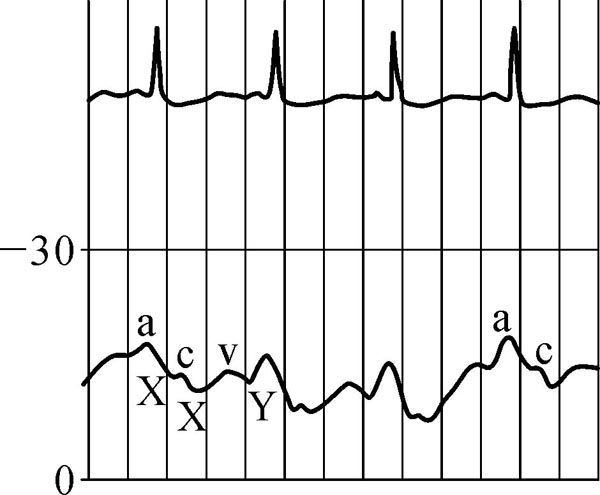
\includegraphics[width=5.91667in,height=2.82292in]{./images/Image00034.jpg}
\end{table}

\paragraph{二、职业性哮喘}

职业性哮喘近年有逐渐增多的趋势。哮喘发作与职业有关者统称职业性哮喘,诊断上应注意发病与职业上有害物质的关系。发病机制主要有:①职业接触物作为变应原,引起主要以IgE介导的速发型超敏反应;②职业有害物质引起药理介质的释放失调;③职业有害物质的非特异刺激反应,其中超敏反应起主导作用。

职业性哮喘的临床特点是:①患者在就业前不存在哮喘;②就业以后发生哮喘(一般可有数月乃至数年的潜伏期);③患病后每从事有害作业时则引起哮喘发作,脱离工作环境或假期休息时则可自行缓解,但再接触后又可发作。

工作环境中的职业性致喘物有400多种,广泛分布于化工、染料、合成纤维、橡胶皮革、纺织、制药、油漆、塑料黏合剂、印刷、冶炼、农药、木材加工、粮食、家禽饲养、农作物种植等。诊断可根据职业史和上述哮喘的特点综合考虑,必要时可行职业变应原支气管激发试验。

\paragraph{三、花粉症}

对花粉过敏者吸入花粉有的可引起气喘。花粉症在我国分布颇广,多由于黄花蒿、臭蒿、艾蒿、茵陈蒿等蒿属植物花粉所引起。此病与支气管哮喘的主要不同点是:①此病发作于花粉散发季节,且多在清晨、晴朗有风之时;②患者常伴有过敏性上呼吸道炎的表现,如流清涕、打喷嚏、鼻塞、眼和鼻奇痒,少数患者可有荨麻疹;③鼻黏膜分泌物涂片检查可发现大量嗜酸性粒细胞。以花粉作鼻黏膜激发试验,阳性率较高,有诊断意义。但应注意有的患者合并有支气管哮喘。

\paragraph{四、变应性支气管肺曲霉病(allergic bronchopulmonary}
aspergillosis,ABPA)

多由烟曲霉引起的气道高反应性疾病。对曲霉过敏者吸入大量孢子后,阻塞小支气管,引起短暂的肺不张和喘息发作,亦可引起肺部反复游走性浸润。患者表现为呼吸困难、喘息、畏寒、发热、乏力、刺激性咳嗽、咳棕黄色脓痰,偶带血。痰中有大量嗜酸性粒细胞及曲霉丝,烟曲霉培养阳性。哮喘样发作为其突出的临床表现,一般解痉平喘药难以奏效,外周血嗜酸性粒细胞增多。典型X线胸片为上叶短暂性实变或不张,可发生于双侧。胸部HRCT呈“近端”或中央支气管囊状扩张及壁增厚征象。诊断标准见第3.1.7节。

\subsubsection{7.2.3 间质性肺疾病}

间质性肺疾病(ILD)是一组主要累及肺间质、肺泡及(或)细支气管的肺部弥漫性疾病,目前已包括200多个病种,按病因明确与否分为病因已明和病因未明两大类,各病种的发病机制有显著区别,但临床上均表现为渐进性劳力性呼吸困难,限制性通气功能障碍伴弥散功能降低,低氧血症。胸部影像学显示双肺弥漫性病变,晚期发展为弥漫性肺纤维化和蜂窝肺,导致呼吸衰竭。

\paragraph{一、尘 肺}

尘肺是在生产活动中长期吸入生产性粉尘所引起的肺间质纤维化疾病,常见有硅沉着病(矽肺)、煤工尘肺、石棉肺和慢性铍肺等,重症患者有呼吸困难症状,在肺功能不全后期更为明显(参见第29节)。

\subparagraph{(一)棉尘肺}

棉纺工人发生气喘发作,须考虑是否为棉尘肺。此病的特点是,罹患此病的棉纺工人在每星期日休息之后,星期一再接触棉尘时便出现胸闷、气急、咳嗽、咳痰(部分病例可带血)等症状,但无发热。轻者工作一二天后症状渐缓解,严重者可持续至脱离接触后仍有症状。此病与长期吸入较高浓度的棉尘(尤以用低级棉为原料及粗纺车间工作者较多罹患)有关,是以支气管痉挛为基本病变的过敏性疾病。此病的主要诊断根据:①有职业史及发作的特殊规律;②肺部X线征可表现为慢性支气管炎、肺气肿征,重症者可呈广泛性网织状阴影。

\subparagraph{(二)霉草尘肺}

此病乃因接触潮湿发霉的干草,吸入带有真菌及其孢子的霉草尘所引起,罹患者以农民为多。患者常在接触后2~3小时发生呛咳、胸闷,继而咳出白色泡沫状或黏液性痰,气喘,并常有乏力、畏寒、发热等全身症状,有时出现荨麻疹。听诊双肺有弥漫性哮鸣音。血中嗜酸性粒细胞增多。X线检查可发现肺部短暂性、炎症性片状阴影及支气管周围炎征象。

所谓甘蔗渣肺也是同类疾病,见于接触发霉甘蔗渣的人。

\subparagraph{(三)蘑菇肺}

本病为蘑菇培植者的过敏性肺泡炎,也可见于平菇培植者。本病开始时易被误诊为感冒或支气管炎,主要表现为咳嗽、咳痰、胸痛、胸闷、咽痛、低热等症状,重症者有气短或呼吸困难;可有皮疹与X线肺部阴影。痰及血中常有嗜酸性粒细胞增多。本病可区分为三种临床类型:①高热型,以高热为主要症状;②支气管炎型,以支气管炎症状为主;③轻型:临床症状轻微而X线胸片有异常。X线胸片大多呈弥漫性阴影,少数呈局限性阴影。

\paragraph{二、外源性过敏性肺泡炎}

多数为在工作场所吸入了植物性或动物性有机粉尘所引起,包括农民肺、棉尘肺、霉草尘肺、甘蔗渣肺、蘑菇肺、饲鸽者肺、湿化器和空调器肺、烟草工人肺、木工肺等数十种,发病机制目前尚未完全明确,但抗原-抗体复合物和T细胞介导的免疫反应是主要的发病机制,尤其后者更为重要。

临床特点:①患者发作的症状严重程度与机体对吸入抗原的免疫反应、粉尘的抗原性、接触强度、次数及持续时间有关,可为急性、亚急性或慢性发作。②急性发作者一般在吸入大量抗原4~8小时后发作,表现为呼吸困难、干咳、胸闷,可有畏寒寒战、高热、全身不适等症状,脱离粉尘接触后1~3天内症状自然消失,少数可持续1周左右;亚急性常由急性发展而来,症状可持续数日或数周;慢性者起病隐匿,咳嗽、呼吸困难等进行性加重,常因不能及时诊治或脱离有机粉尘环境而发展为慢性肺间质纤维化,导致慢性肺心病。③用特异性抗原溶液行吸入激发试验或抗原皮肤试验常阳性。

部分急性外源性过敏性肺泡炎患者在吸入抗原后可出现哮喘症状,应与支气管哮喘鉴别,参考表\ref{tab3-4}。

\begin{table}[htbp]
\centering
\caption{外源性过敏性肺泡炎与支气管哮喘的鉴别}
\label{tab3-4}
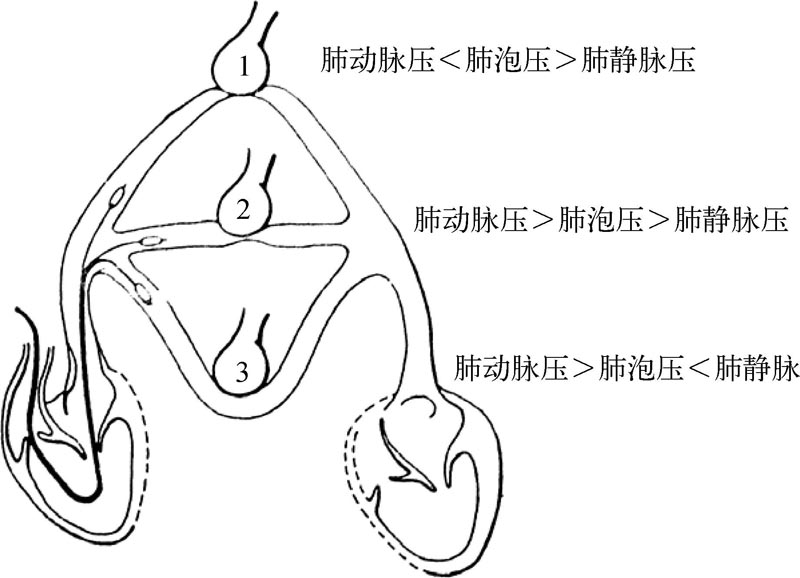
\includegraphics[width=5.90625in,height=4.09375in]{./images/Image00035.jpg}
\end{table}

\paragraph{三、特发性间质性肺炎}

特发性间质性肺炎(IIPs)是一组原因不明的肺间质性疾病,其分类与命名几经修改,目前的分类同时强调了临床-放射-病理诊断,包括了特发性肺纤维化(IPF)、非特异性间质性肺炎(NSIP)、隐源性机化性肺炎(COP)、急性间质性肺炎(AIP)、呼吸性细支气管炎间质性肺疾病(RBILD)、脱屑性间质性肺炎(DIP)、淋巴细胞性间质性肺炎(LIP)、特发性胸膜肺实质纤维弹性组织增生症(IPPF)和未分类特发性间质性肺炎(UCIIP)各自不同的实体疾病。这组疾病的临床表现非常相似,缺乏诊断特异性,但预后和治疗反应的差异性很大,故需要结合临床、放射学、肺生理功能、支气管肺泡灌洗和组织病理学等综合评估,才能明确最后诊断,并注意排除结缔组织疾病、药物、职业、感染等所致的继发性间质性肺疾病。

\subparagraph{(一)特发性肺纤维化}

特发性肺纤维化(IPF)是指原因不明并以普通型间质性肺炎(UIP)为特征性病理改变的一种慢性炎症性间质性肺疾病,占所有IIPs的60\%以上,主要表现为弥漫性肺泡炎、肺泡单位结构紊乱和肺纤维化。临床表现:①发病年龄多在中年以上,男∶女≈2∶1,儿童罕见;②起病隐袭,主要表现为干咳、进行性呼吸困难,活动后明显;③本病少有肺外器官受累,但可出现全身症状,如疲倦、关节痛及体重下降等,发热少见;④50\%左右的患者出现杵状指(趾),多数患者双肺下部可闻及Velcro啰音;⑤晚期出现发绀,偶可发生肺动脉高压、肺心病和右心功能不全等。胸片显示双肺弥漫的网格状或网格小结节状浸润影,以双下肺和外周(胸膜下)明显。HRCT是IPF诊断流程中的重要组成部分。HRCT上UIP的特征为胸膜下和肺基底部的网格状阴影和蜂窝影,常伴有牵张性支气管扩张,尤其是蜂窝影对IPF的诊断有很重要的意义。肺功能表现为限制性通气功能障碍和弥散量减少。UIP的组织病理学特征和主要诊断标准是在低倍镜下病变的不均一性,即瘢痕形成和蜂窝样改变的纤维化区域与病变轻微或正常的肺实质区域交替出现。通过有丰富ILD诊断经验的呼吸内科医生、影像科医生和病理科医生之间的多学科讨论,仔细排除其他可能的病因,是获得准确诊断最为重要的环节。诊断IPF需要符合:①排除其他已知病因的ILD(例如家庭和职业环境暴露、结缔组织疾病和药物);②未行外科肺活检的患者,HRCT呈现UIP表现;③接受外科肺活检的患者,HRCT和肺活检组织病理类型符合特定的组合。

IPF的诊断标准分为有外科(开胸/胸腔镜)肺活检资料和无外科肺活检资料。有外科肺活检资料:①肺组织病理学表现为UIP特点;②除外其他已知病因所致的间质性肺疾病,如药物、环境因素和风湿性疾病等所致的肺纤维化;③肺功能异常,表现为限制性通气功能障碍及(或)气体交换障碍;④胸片和高分辨CT(HRCT)可见典型的异常影像。无外科肺活检资料(临床诊断):缺乏肺活检资料原则上不能确诊IPF,但如患者免疫功能正常,且符合以下所有的主要诊断条件和至少3/4的次要诊断条件,可临床诊断IPF。

\hypertarget{text00046.htmlux5cux23CHP3-4-5-3-3-1-1}{}
1.主要诊断条件

①除外已知原因的ILD,如某些药物毒性作用、职业环境接触史和风湿性疾病等;②肺功能表现异常,包括限制性通气功能障碍(VC减少,而FEV\textsubscript{1}
/FVC正常或增加)及(或)气体交换障碍[静态/运动时P\textsubscript{(A-a)}
O\textsubscript{2}
增加或DLCO降低];③胸部HRCT表现为双肺网状改变,晚期出现蜂窝肺,可伴有极少量磨玻璃影;④经支气管肺活检(TBLB)或支气管肺泡灌洗液(BALF)检查不支持其他疾病的诊断。

\hypertarget{text00046.htmlux5cux23CHP3-4-5-3-3-1-2}{}
2.次要诊断条件

①年龄>50岁;②隐匿起病或无明确原因进行性呼吸困难;③病程≥3个月;④双肺听诊可闻及吸气性Velcro音。

2011年ATS/ERS/JRS/ALAT更新了关于IPF诊治的询证医学指南,其诊断标准如下:

1.排除其他已知原因的间质性肺疾病(如家庭或职业环境暴露、结缔组织疾病和药物毒性)。

2.未施行外科肺活检的患者HRCT表现为典型UIP型。

3.施行外科肺活检的患者应结合HRCT和外科肺活检病理类型[尤其是HRCT或(和)组织病理学不典型时]。

典型UIP型HRCT诊断标准(所有4个特征):病灶以胸膜下、基底部为主;网格状异常改变;蜂窝肺伴或不伴牵张性支气管扩张;无不符合UIP型所列的CT特征。

UIP型的组织病理学标准(所有4条标准):以胸膜下或间隔旁分布为主的明显纤维化和结构紊乱的证据,伴或不伴蜂窝;肺实质斑片状纤维化改变;出现成纤维细胞灶;无不支持UIP诊断的病理特征。

\subparagraph{(二)非特异性间质性肺炎}

非特异性间质性肺炎(NSIP)为IIPs的一种,病因不清,国内一组8例报道中3例可能与环境暴露(棉尘、沙尘、动物皮毛、挥发性酸性化合物)有关。国外报道多以风湿性疾病为病因。其临床表现和影像学与IPF类似,主要表现为咳嗽、呼吸困难、双下肺可闻及Velcro啰音;胸片表现为中下肺野为主的网状阴影,有时表现为斑片阴影;HRCT显示双肺对称性磨玻璃影或双肺肺泡腔的实变影。

NSIP与IPF临床上的主要鉴别有:①IPF发病年龄(平均57岁)大于NSIP(平均49岁)。②IPF多见于男性;NSIP多见于女性。③IPF起病多隐匿,就诊时通常已有1~2年病史;NSIP起病多呈亚急性,从出现症状到确诊很少超过1年。④IPF患者发热很少见,杵状指多见;NSIP可有发热(22\%~33\%),杵状指少见。⑤IPF对糖皮质激素治疗不敏感;NSIP对激素反应良好。⑥IPF预后差,死亡率60\%~90\%;NSIP预后良好,死亡率0\%~29\%。

\paragraph{四、结节病}

结节病是一种多系统器官受累的肉芽肿性疾病,常侵犯肺、双侧肺门淋巴结,也可侵犯其他器官,病因尚未十分明确,可能与遗传因素、特殊病原体的感染(病毒、支原体、真菌等)、自身免疫、吸入无机物(铝、锆、滑石)或有机物(枫树粉、黏土)等有关。早期呼吸道症状较轻,多为干咳,无痰或少痰,后期可因肺纤维化导致呼吸困难。(参见第26.1节)。

\paragraph{五、肺嗜酸性粒细胞浸润症}

肺嗜酸性粒细胞浸润症是一组由嗜酸细胞浸润引起的肺部病变,常伴有外周血嗜酸性粒细胞增多。病因与发病机制尚不完全清楚,可能与变态反应或免疫反应异常有关。临床上主要表现有不同程度的胸闷、咳嗽、喘息、呼吸困难、乏力、低热等症状。

\subparagraph{(一)单纯性肺嗜酸性粒细胞浸润症}

又称吕弗勒综合征,其病因与发病机制尚不完全清楚,可能与寄生虫感染(蛔虫、钩虫、丝虫、绦虫、姜片虫、阿米巴原虫等)和某些药物(对氨基水杨酸、阿司匹林、磺胺制剂等)引起的肺部Ⅰ型和Ⅲ型变态反应有关,其他病因可能为吸入花粉、真菌孢子等。

本病国内报道颇多,其临床表现一般较轻,患者有全身不适、乏力、低热、干咳等症状,大多咳少量的黏稠痰液。少数患者症状较重,表现为高热、哮喘或呼吸困难。体检胸部体征轻微,可有少量干湿音或全无体征,与肺部X线摄片所见不相称。血象白细胞总数正常或稍增高,分类计数嗜酸性粒细胞明显增加,多数在10\%~20\%,偶达70\%~80\%,绝对计数达(1.0~2.5)×10\textsuperscript{9}
/L。血象改变通常在发病10~15天后消失。肺部X线征极不一致,可呈片状、圆形、粟粒样、结节状、条状或不规则的阴影,病灶附近肺纹理增加;有时肺部X线征呈游走性变化,此起彼伏,并多于发病6~12天后消失,很少延长至一个月以上。

诊断本病的主要依据是:①病程短促与良性经过;②上述的症状与体征;③外周血嗜酸性粒细胞增多;④X线检查肺部有短暂性浸润阴影,消散后不留痕迹。

在鉴别诊断上本病须与肺结核、肺炎支原体肺炎、不完全性大叶性肺炎、热带肺嗜酸性粒细胞增多症等相区别。因X线摄片上可能出现大片阴影,类似浸润性肺结核或干酪样肺炎,或呈粟粒样阴影而类似粟粒型肺结核,或偶尔肺部浸润消散过程中出现假性空洞而类似肺结核空洞形成。根据肺结核的全身中毒症状较重,X线复查肺部阴影不可能在短期内消散,血象中无嗜酸性粒细胞增多,痰中可查到抗酸杆菌等现象,一般鉴别不难。肺炎支原体肺炎的肺部阴影虽可于较短期内消散,但无嗜酸性粒细胞增多,且常有较高效价的冷凝集反应。大叶性肺炎不仅无嗜酸性粒细胞增多,而且症状较重和体征明显,据此可与本综合征相区别。

本综合征与热带肺嗜酸性粒细胞增多症的鉴别诊断参考表\ref{tab5-5}。

\subparagraph{(二)热带嗜酸性粒细胞浸润症}

本病病情严重时可有哮喘样发作,也可以哮喘样发作突然起病(参见第16节)。

\subparagraph{(三)慢性嗜酸性粒细胞性肺炎}

慢性嗜酸性粒细胞性肺炎(CEP)病因与发病机制不清楚,可能与自身免疫有关。本病病程较单纯性肺嗜酸性粒细胞增多症长,通常为2~6个月,甚至一年以上。多见于中青年女性,临床上起病缓慢,常见发热、干咳或咳少量黏稠样痰、盗汗、体重减轻;约1/3患者合并哮喘,可有喘息、进行性呼吸困难以及呼吸衰竭。外周血嗜酸性粒细胞多增高,比例可达20\%~70\%。胸部X线显示非段或叶性分布的片状阴影,常为外侧外带分布,出现特征性的“肺水肿反转征”,阴影可有一定的游走性,予糖皮质激素治疗后阴影迅速消失。

\paragraph{六、嗜酸性肉芽肿性多血管炎}

原称为变应性肉芽肿性血管炎,又称Churg-Strauss综合征(CSS),是一种以多器官系统发生肉芽肿性血管炎为特征的少见疾病,肺部血管最易受累。病因与发病机制均不清楚,主要临床表现为支气管哮喘、过敏性鼻炎、外周血嗜酸性粒细胞增多和多器官组织坏死性血管炎,周围形成肉芽肿及大量嗜酸性粒细胞浸润为特征。

1990年美国风湿病协会提出本病的6项诊断标准为:①哮喘;②外周血嗜酸性粒细胞增多,分类计数>10\%;③单发性或多发性神经病变;④游走性或一过性肺浸润;⑤鼻窦病变;⑥组织活检证实有血管外嗜酸性粒细胞浸润。凡患者有上述6项标准中4项或以上者可诊断本病,诊断敏感性85.0\%,特异性99.7\%。

本病主要须与Wegener肉芽肿相鉴别:本病主要表现为支气管哮喘,过敏性鼻炎,鼻腔病变多为弥漫性鼻黏膜肿胀、鼻息肉,累及肾脏时病变程度较轻;而Wegener肉芽肿鼻腔病变多为鼻溃疡、凝固性或液化坏死性肉芽肿,肺内浸润易形成空洞,且肾损害较严重,而没有支气管哮喘和外周血嗜酸性粒细胞增高。

\paragraph{七、淋巴细胞间质性肺炎}

淋巴细胞间质性肺炎以渐进性活动后气促、咳嗽、消瘦为主征,严重者呼吸困难与发绀。体检双下肺可闻小水泡音及爆裂音。X线胸片示双侧中、下肺野以中内带为主的广泛网状阴影,夹杂以小结节阴影。经纤支镜下肺组织病理活检可确诊。泼尼松治疗疗效好。

淋巴细胞性间质性肺炎(LIP)是临床少见疾病,2002年美国胸科协会(ATS)及欧洲呼吸协会(ERS)发布的国际多学科共识意见将特发性间质性肺炎分为七类,LIP为其中之一。LIP起病隐匿,病程长,多数患者为女性,男女的比例约为1∶2,发病年龄从40~70岁不等,诊断时的平均年龄在52~56岁。呼吸系统的主要症状是干咳、逐渐加重的呼吸困难,偶有发热、盗汗、体重下降。胸部查体可发现双肺底爆裂音,杵状指(趾)少见。外周及纵隔淋巴结肿大及脾大很少见。肺功能通常提示限制性通气功能障碍及(或)弥散功能减低。高分辨CT表现为小叶中心性结节、胸膜下结节、双下肺为主的毛玻璃样斑点影、支气管血管束增厚。LIP的诊断实质上是病理诊断,LIP的病理特点是多克隆的成熟的小淋巴细胞弥漫浸润肺间质,包括小叶间隔、肺泡间隔,细胞成分以淋巴细胞为主,伴有浆细胞、组织细胞、上皮细胞等。

\paragraph{八、原发性呼吸道淀粉样变性}

淀粉样变性是一组表现各异的临床综合征,共同点是组织或器官的细胞外淀粉样蛋白质沉积,可累及全身器官,但如仅累及呼吸道时,则称原发性呼吸道淀粉样变性。本病少见,起病隐袭缓慢,主要表现为咳嗽、咳痰、进行性呼吸困难,可有咯血。纤支镜下活检可作出诊断。

国内曾报道三例患者,均为男性,纤支镜检查显示不同程度气管及(或)支气管不规则狭窄,不同叶、段支气管管腔狭窄至闭塞,管腔内有小结节状突起,黏膜水肿,充血,有出血或出血倾向。活检病理检查证实支气管黏膜下淀粉样变性:苏木素伊红染色黏膜内有大片絮状不规则无细胞的嗜伊红物质沉积,刚果红染色呈玫瑰红色,有双折光性,在偏光显微镜下刚果红阳性处呈绿色。

\paragraph{九、肺泡蛋白质沉积症}

本病可引起进行性气促,严重者可呈明显呼吸困难和发绀。乃由于肺泡及细支气管内充满PAS染色阳性的颗粒状类蛋白质物质所致(参见第15节)。

\subsubsection{7.2.4 阻塞性病变}

\paragraph{一、慢性阻塞性肺疾病}

慢性阻塞性肺疾病(COPD)是一种具有气流受限特征的肺部疾病,气流受限不完全可逆,呈进行性发展。确切的病因还不十分清楚,但认为与肺部对有害气体或有害颗粒的异常炎症反应有关。支气管哮喘(其为一种特殊的气道炎症性疾病,其气流受限具有可逆性)和一些已知病因或具有特征病理表现的气流受限疾病(如肺囊性纤维化、弥漫性泛细支气管炎、闭塞性细支气管炎等)不属于COPD的范畴。

COPD的起病缓慢,病程较长,主要症状为慢性咳嗽、咳痰,一般为白色黏液或浆液性泡沫性痰;气短或呼吸困难,早期在劳力时出现,以后呈进行性加重,是COPD的标志性症状;部分患者特别是重度患者或急性加重时出现喘息、胸闷;晚期患者有体重下降,食欲减退等。早期体征可无异常,随疾病进展可出现典型肺气肿体征:桶状胸,肺部叩诊过清音,心浊音界缩小,肺下界和肝浊音界下降,双肺呼吸音减弱,呼气延长,部分患者可闻及干啰音及(或)湿啰音。

COPD的诊断可根据吸烟等高危因素史、临床症状、体征及肺功能检查等综合分析确定。诊断的必备条件是肺功能检查显示不完全可逆的气流受限,即吸入支气管舒张药后FEV\textsubscript{1}
/ FVC<70\%及FEV\textsubscript{1}
<80\%预计值。无肺功能检查仪时可行用力呼气时间听诊法进行估计:被检者深吸气后屏气,然后用力尽快将气呼出。检查者将听诊器置于患者气管或胸骨上段,计算用力呼气时间,从呼气开始至呼气终止这段时间为最大呼气时间。正常不超过4秒,轻度阻塞者通常在6秒以内,中、重度阻塞者在6秒以上。

\paragraph{二、阻塞性肺不张}

急性大片阻塞性肺不张起病急骤,常有呼吸困难、心动过速,有时伴有休克现象;缓慢发展的肺不张,患者可无自觉症状。

阻塞性肺不张由于支气管内黏膜高度水肿、分泌物、瘢痕收缩、异物、支气管恶性或良性肿瘤、结核病变等阻塞支气管腔所引起。

大片阻塞性肺不张的主要体征是患侧胸廓凹陷,肋间变窄,呼吸运动减弱,膈肌升高,气管、心脏与纵隔向患侧移位。患侧部位叩诊可呈浊音,呼吸音减弱或消失;但也有叩诊无浊音者,其原因是由于邻近肺组织产生代偿性肺气肿。诊断主要根据临床表现与X线检查。

急性阻塞性肺不张往往伴有感染,引起发热、咳嗽,须与大叶性肺炎相区别。后者常由肺炎链球菌感染所致,有寒战、高热、胸痛,咳嗽较显著,可咳出铁锈色痰,无气管与纵隔的移位。X线检查有助于二者的区别。

阻塞性肺不张亦需与压迫性肺不张相鉴别,后者是由于胸腔积液、气胸,肺内或胸腔内肿瘤,肺包虫病,胸廓畸形,呼吸肌或膈肌麻痹,纵隔肿瘤,淋巴结肿大,扩大的心脏,胸内甲状腺,膈疝,主动脉瘤及腹腔巨大肿瘤、大量腹水使膈肌升高等所引起。其体征与阻塞性肺不张不同,因不同病因而异。

\paragraph{三、弥漫性泛细支气管炎}

弥漫性泛细支气管炎是一种原因不明的、以弥漫存在于两肺细支气管和呼吸性细支气管区域并累及管壁全层的慢性炎症为特征的疾病。1969年首先由日本学者山中、本间、谷木等提出,可表现为慢性咳嗽、多痰和劳力性呼吸困难,并伴有气流受限。慢性的咳嗽和较多的脓痰等症状的进展多见于20~50岁人群,随后逐渐出现劳力性呼吸困难。肺部听诊可闻及爆裂音、哮鸣音。胸部CT表现为弥漫性小结节影和线状阴影,小叶中心性小颗粒状,与胸壁有少许间隔为其特点;小支气管和细支气管扩张,以两肺下叶最明显;支气管壁增厚;易合并中叶和舌叶肺不张。

1998年日本厚生省临床诊断标准:

\subparagraph{1.必要条件}

①持续咳嗽、咳痰及活动时呼吸困难;②合并有慢性鼻窦炎或有既往史;③胸部X线见两肺弥漫性散在分布的颗粒样结节状阴影或胸部CT见两肺弥漫性小叶中心性颗粒样结节状阴影。

\subparagraph{2.参考条件}

①胸部间断性湿啰音;②第1秒用力呼气容积与用力肺活量比值(FEV\textsubscript{1}
/ FVC\%)<70\%,动脉血氧分压(PaO\textsubscript{2}
)<80mmHg;③血清冷凝集试验效价>1∶64。

\subparagraph{3.临床诊断}

(1)临床确诊:必要条件①+②+③加参考条件中>2项。

(2)临床高度可疑诊断:必要条件①+②+③。

(3)临床可疑诊断:必要条件①+②。

临床上要与慢性阻塞性肺疾病、支气管扩张、支气管哮喘等疾病鉴别。

\subsubsection{7.2.5 其他原因}

\paragraph{一、急性肺损伤与急性呼吸窘迫综合征}

急性肺损伤(ALI)/急性呼吸窘迫综合征(ARDS)是指由心源性以外的各种肺内外致病因素导致的急性、进行性缺氧性呼吸衰竭。ALI和ARDS具有性质相同的病理生理改变,ARDS是严重的ALI。其主要病理基础是由多种炎症细胞(巨噬细胞、中性粒细胞和淋巴细胞等)介导的肺脏局部炎症反应和炎症反应失控所致的肺毛细血管膜损伤。主要病理特征为由于肺微血管通透性增高而导致的肺泡渗出液中富含蛋白质的肺水肿及透明膜形成,可伴有肺间质纤维化。病理生理改变以肺顺应性降低,肺内分流增加及通气血流比例失调为主。2012年由欧洲危重病医学会(ESICM)与美国胸科学会(ATS)组成的联合委员会于2012年发表了ARDS柏林定义。根据柏林定义,ARDS是一种急性弥漫性肺部炎性反应,可导致肺血管通透性升高,肺重量增加,参与通气的肺组织减少。

临床表现为呼吸频数和呼吸窘迫、顽固性低氧血症,而动脉血二氧化碳分压(PaCO\textsubscript{2}
)正常,早期肺部听诊无明显异常,病情进展肺部可听到干、湿啰音。胸部X线显示双肺弥漫性浸润影,后期常并发多器官功能衰竭。

ARDS的高危因素包括直接肺损伤因素(严重肺感染、胃内容物吸入、肺挫伤、吸入有毒气体、淹溺、氧中毒等)和间接肺损伤因素(脓毒症、严重的非胸部创伤、重症胰腺炎、大量输血、体外循环、DIC等)。

1994年欧美共识会议(AECC)发表ARDS诊断标准:①急性起病;②氧合指数(PaO\textsubscript{2}
/ FiO\textsubscript{2}
)≤200mmHg(1mmHg=0.133kPa,不考虑PEEP因素);③正位胸片显示双肺斑片状浸润影;④肺动脉楔压(PAWP)≤18mmHg,或无左心房压力增高的临床证据。2000年中华医学会呼吸病学分会起草提出了ALI/ARDS的诊断标准(草案)与AEEC标准基本相同。

近年来临床研究显示,欧美共识会议诊断标准的敏感性为84\%,而特异性仅为51\%。2011年欧洲重症医学会柏林会议在ARDS流行病学、病理生理学和临床研究基础上,提出了ARDS柏林新定义。该定义将ARDS患者分为轻、中、重3个层次,其中轻度取代了ALI,建议废除ALI的命名。其临床诊断的有效性和准确性尚有待进一步证实(表\ref{tab3-5}\footnote{a:胸片或CT;b:如海拔>1000m,按以下公式纠正:[PaO\textsubscript{2}
/FiO2×(大气压/760)];c:轻度ARDS可用无创通气})。

\begin{table}[htbp]
\centering
\caption{急性呼吸窘迫综合征的柏林定义}
\label{tab3-5}
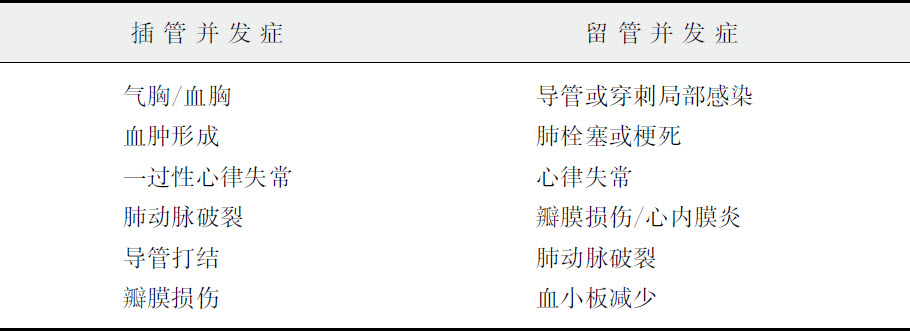
\includegraphics[width=5.89583in,height=2.01042in]{./images/Image00036.jpg}
\end{table}

ARDS诊断时须排除大片肺不张、自发性气胸、上气道阻塞、急性肺栓塞和心源性肺水肿等。与心源性肺水肿的鉴别可根据下列几点:

1.心源性肺水肿的呼吸困难与体位有关,而ARDS则不太明显。

2.心源性肺水肿咳粉红色泡沫样痰,而ARDS的血痰多非泡沫性,而为稀血水样。

3.心源性肺水肿对强心苷、利尿药和血管扩张药有较佳的治疗反应,而ARDS即使吸入高浓度氧疗效不显著。

4.心源性肺水肿湿啰音多集中于肺底,而ARDS的湿啰音分布较广泛,且音调较高,常呈“爆裂音”。

5.心源性肺水肿X线胸片异常阴影与相应的临床表现几乎同时出现,对及时的急救治疗反应常迅速;而ARDS的X线胸片所见疑似肺泡性水肿,但经积极抢救X线征象在数日内无明显好转。鉴别困难时,可通过超声心动图检测心室功能等作出判断并指导此后的治疗。

\paragraph{二、肝肺综合征}

肝肺综合征(HPS)是指肝功能不全引起肺血管扩张、肺气体交换障碍导致的低氧血症及其一系列的病理生理变化和临床表现。常把肝功能不全、肺血管扩张和低氧血症三联症称为HPS。HPS常见于肝炎后肝硬化、酒精性肝硬化及其他原因肝硬化,也可见于慢性活动性肝炎、急性暴发性肝炎、胆汁淤积、非肝硬化性门脉高压(如门体静脉或脾肾静脉吻合手术后)等。国内曾报道两组分别为6例和16例的HPS,均在乙型肝炎、丙型肝炎、酒精性肝病、Wilson病所致的肝硬化基础上发生。

HPS临床上除了肝病的一般表现外,还存在与肝病有关的低氧血症,表现为活动性呼吸困难、发绀、杵状指,其原理是由于肺血管扩张引起的通气/灌注和弥散功能失调。目前认为肺内血管扩张的发生与肺血管扩张物质(如血管活性肠肽等)在肝功能不全时不能被灭活,或经门体分流和淋巴通道进入肺循环,也可能是内皮素、血管紧张素Ⅰ等缩血管物质的缺乏或被抑制,或肺血管内皮细胞对缩血管物质敏感性的下降,致使原关闭的无功能性毛细血管前交通支开放,以及原本正常的低氧性肺血管收缩功能发生障碍。HPS的缺氧表现为直立位低氧,即由卧位改变为直立位时呼吸困难和发绀加剧,PaO\textsubscript{2}
下降10mmHg以上,这是因为肺血管扩张主要位于两肺基底部,直立位时因重力作用影响,流经肺下野的血流量增多,致使肺内右至左分流量增多,氧合障碍进一步加重,缺氧加剧。

确定肺血管扩张是诊断HPS的关键,符合下列条件的可以诊断为HPS:①急、慢性肝脏疾病;②没有原发性心肺疾病,胸片正常或有间质结节状阴影;③肺气体交换异常,有或无低氧血症,P\textsubscript{(A-a}
)O\textsubscript{2}
梯度>15mmHg;④对比增强超声心动描记术(CTTE)及(和)肺灌注扫描,肺血管造影存在肺血管扩张及(或)肺内血管短路;⑤直立位缺氧、气短、发绀,肺骨关节病。诊断标准:肝硬化基础上+微发泡试验阳性+直立位低氧血症(PaO\textsubscript{2}
<70mmHg,即可诊断HPS。如肝硬化基础上+微发泡试验阳性+无直立位低氧血症,说明有肺血管扩张,尚未达到HPS。

\protect\hypertarget{text00047.html}{}{}

\subsection{7.3 胸膜疾病}

\subsubsection{一、自发性气胸}

自发性气胸多以骤然发生的患侧胸痛与呼吸困难起病。严重者(多为张力性气胸)呈进行性呼吸困难、发绀,甚至出现休克。体检发现患侧胸廓饱满,呼吸运动减弱,触觉语颤减弱或消失,叩诊呈鼓音,听诊肺泡呼吸音减弱或消失。气管、心脏与纵隔向健侧移位。临床上一经诊断为张力性自发性气胸,不必等待X线诊断,应立即进行胸腔穿刺排气。

自发性气胸可分成原发性和继发性。继发性发生在有基础肺疾病的患者,由于病变引起细支气管不完全阻塞,形成肺大疱破裂,如肺结核、COPD、肺癌、肺脓肿、尘肺等;原发性发生在无基础肺疾病的健康人,多见于瘦高体型的男性青壮年,常规X线检查肺部无显著病变,但胸膜下可有肺微小疱,多在肺尖部。

根据脏层胸膜破裂情况不同及其发生后对胸腔内压力的影响,自发性气胸通常分为三种临床类型:闭合性(单纯性)、交通性(开放性)及张力性(高压性),见表\ref{tab3-6}。

\begin{table}[htbp]
\centering
\caption{各类型自发性气胸的鉴别}
\label{tab3-6}
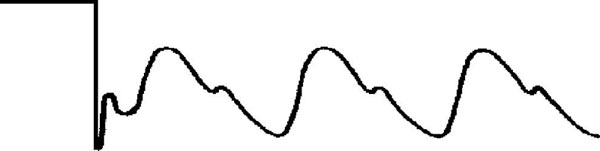
\includegraphics[width=5.91667in,height=2.65625in]{./images/Image00037.jpg}
\end{table}

继发性自发性气胸中最常由肺结核引起,肺结核病灶破裂的特点是:①患者常有发热等结核感染中毒症状;②如有胸腔积液,常为脓性,量常较多;③肺部X线检查通常无肺气肿或肺大疱。

自发性气胸须与肺大疱相区别,主要根据:①后者症状不明显或较轻;②胸部X线检查肺大疱的气腔位于肺实质中,因此在肺尖和肋膈角仍可见有肺组织,并可见气腔内有纤维条索状影像走向肺门,而气胸的气体位于胸腔内,肺组织被推向肺门;③肺大疱有整齐、致密而菲薄的线状泡壁,气腔呈圆形或椭圆形。

\subsubsection{二、大量胸腔积液}

由于大量胸腔积液,压迫肺组织产生压迫性肺不张,使肺呼吸面积减少;同时使纵隔向健侧移位,以致发生呼吸困难。呼吸困难一般发生较缓慢。其严重程度取决于积液产生的速度及其量的大小。急速大量积液时,呼吸困难较明显;积液缓慢发生者,有时可因患者逐渐适应而无呼吸困难。胸腔积液的病因较繁杂(参见第33节)。

\protect\hypertarget{text00048.html}{}{}

\subsection{7.4 纵隔疾病}

\subsubsection{一、急性纵隔炎(参见第33节)。}

\subsubsection{二、慢性纤维性纵隔炎}

慢性纤维性纵隔炎多继发于化脓性或结核性纵隔炎之后,病理改变为纤维组织增生与瘢痕收缩,病变可为广泛性或局限性,症状因纵隔组织受累不同而表现不一。如压迫气管、支气管,则出现气短与呼吸困难;如压迫上腔静脉,则出现上腔静脉阻塞综合征(参见第38节);如压迫喉返神经,则出现声音嘶哑;压迫食管则引起吞咽困难。

\subsubsection{三、纵隔肿瘤及囊肿}

纵隔肿瘤及囊肿发展到一定阶段,压迫或侵犯气管或大支气管时,可引起不同程度的呼吸困难(参见第27.1节)。

\subsubsection{四、纵隔气肿}

严重的纵隔气肿可引起呼吸困难(参见第33节)。

\protect\hypertarget{text00049.html}{}{}

\subsection{7.5 胸廓运动及呼吸肌功能障碍}

胸廓运动受限、呼吸肌和膈肌麻痹、膈高位等皆可使肺呼吸面积减少,而引起呼吸困难。严重的胸廓畸形、肋软骨骨化及硬皮病等均可使胸廓活动受限制;呼吸肌及膈肌麻痹,常由于脊髓灰质炎,脊髓创伤、脑膜炎或脊柱结核所致的神经根病变,多发性神经根神经炎,白喉,重症肌无力等所引起;主动脉瘤可压迫左侧膈神经,肺门部肿瘤或转移瘤也可侵犯膈神经而使膈肌麻痹;膈肌高位常见于妊娠后期、高度的腹水、人工气腹或鼓肠、巨大的腹腔内肿瘤等。

膈肌麻痹

膈肌麻痹分为单侧膈肌麻痹和双侧膈肌麻痹,一般来说单侧膈肌麻痹远多于双侧膈肌麻痹。常见发病原因包括创伤、压力相关、炎症以及神经源性和特发性。其临床表现多种多样,从无症状至呼吸衰竭均可出现,部分患者可表现为重度劳累性呼吸困难以及平卧位呼吸困难,尤其是在夜间快速动眼期可以出现夜间低氧血症和高碳酸血症。因为膈肌麻痹的临床症状无显著特殊性,所以临床上常常误诊为冠状动脉粥样硬化性心脏病、肺炎、肺不张等疾病,据报道平均误诊时间可达2年左右。影像学检查对于诊断膈肌麻痹尤其是单侧膈肌麻痹意义重大,但是对于双侧膈肌麻痹则误诊率高。最大跨膈压检测是诊断膈肌麻痹的金指标。

\protect\hypertarget{text00050.html}{}{}

\subsection{7.6 肺血管病变}

\subsubsection{一、肺栓塞}

肺栓塞和肺梗塞二者有不同的涵义。体循环静脉中或右心的栓子,沿血流进入并堵塞肺动脉或其分支,称为肺栓塞。栓塞部分的肺组织,可因缺氧、坏死而形成肺梗塞。肺栓塞并非都引起肺梗塞。肺梗塞在病理解剖上属于出血性梗塞范畴。

肺栓塞(PE)是以各种栓子阻塞肺动脉系统为其发病原因的一组疾病或临床综合征的总称,包括肺血栓栓塞症(PTE)、脂肪栓塞综合征、羊水栓塞、空气栓塞等。我国由于既往对此病认识不足,临床上经常误诊、漏诊,近年来的研究表明,肺栓塞在我国并非少见。

肺栓塞常见的危险因素和基础病因包括深静脉血栓形成(DVT)、恶性肿瘤、各种心脏病、结缔组织病(系统性红斑狼疮、抗磷脂综合征等)、肾病综合征、外伤、手术和妊娠等。国内一组63例和一组39例的肺栓塞的报道显示最常见的临床症状为呼吸困难、咯血、心悸、胸痛、咳嗽,部分患者有发热、发绀、晕厥等。

\paragraph{(一)肺血栓栓塞症}

PTE为来自静脉系统或右心的血栓阻塞肺动脉或其分支所致的疾病,以肺循环和呼吸功能障碍为其主要临床和病理生理特征。引起PTE的血栓可以来源于下腔静脉径路、上腔静脉径路或右心腔,其中大部分来源于下肢深静脉,特别是从腘静脉上端到髂静脉段的下肢近端深静脉(约占50\%~90\%)。PTE为PE的最常见类型,占PE中的绝大多数,通常所称PE即指PTE。

PTE的临床症状多种多样,均缺乏特异性,症状的严重程度亦有很大差别,可以从无症状到血流动力学不稳定,甚或发生猝死。常见症状包括:呼吸困难及气促、胸痛、晕厥、烦躁不安、惊恐甚至濒死感、咯血、发热等。体检可见呼吸急促、脉速、低血压甚至休克,发绀、颈静脉充盈或搏动、肺部可闻及哮鸣音及(或)细湿啰音,胸腔积液时有相应体征。体检时要注意有否下肢肿胀、压痛、浅静脉扩张、皮肤色素沉着等。

如怀疑PTE,尽快行血浆D-二聚体检测,含量<500mg/L可排除诊断;超声检查可以提示PTE和排除其他疾病;放射性核素肺通气/灌注扫描具有较为重要的诊断或排除诊断意义;螺旋CT、电子束CT或MRI有助于发现肺动脉内血栓的直接证据,已成为临床上经常应用的重要检查手段;肺动脉造影是诊断的“金标准”和参比方法,但为有创性,费用较高。以上检查可根据具体情况选用。

PTE须与急性心肌梗死以及大叶性肺炎相鉴别。急性心肌梗死疼痛多位于心前区,患者有高血压或动脉粥样硬化病史,体温增高较迟于PTE,多在第二、三天才出现,如有咯血与肺局部体征,则更不支持急性心肌梗死的诊断。PTE的典型心电图呈S\textsubscript{Ⅰ}
Q\textsubscript{Ⅲ} T\textsubscript{Ⅲ}
征(即Ⅰ导联S波加深,Ⅲ导联出现Q/q波及T波倒置),往往有完全或不完全性右束支传导阻滞,肺型P波,电轴右偏及顺钟向转位等,如病情好转,心电图改变在较短期间恢复正常,与急性心肌梗死特征性的心电图改变及动态衍变不同,且急性心肌梗死有动态的心肌酶学水平改变。X线检查PTE可发现肺部阴影、肺底浸润或肋膈角模糊阴影,而急性心肌梗死如无发生心力衰竭出现肺水肿则一般没有肺部阴影。大叶性肺炎先有寒战、高热,其后才发生胸痛、咳铁锈色痰,可有唇周疱疹,有典型的胸部X线大叶实变阴影,与PTE不同。

\paragraph{(二)羊水栓塞}

羊水栓塞少见,为一种产科急症,为妊娠期羊水中胎儿产物(胎儿的上皮、毛发、胎脂、黏蛋白、胎粪)进入母体循环而引起。常表现为产妇在破水后不久,突然出现呼吸困难、发绀、抽搐,或兼有休克、昏迷等症状,临床医师应立即考虑此病的可能性,并马上进行诊断与抢救。

发病机制主要由于羊水中胎儿产物作为栓子进入母体循环后可引起肺血管栓塞、变态反应性休克、凝血机制障碍甚至并发弥散性血管内凝血(DIC),影响脏器供血和脏器功能。患者大多数为足月妊娠的中年经产妇,在伴有子宫强烈收缩的情况下发病。由于其发生极其迅速、凶险,病理生理学机制复杂,加之临床医生对它缺乏足够的认识,往往不能及时作出处理,导致母婴死亡率都很高,产妇多因休克、肺水肿或产后大出血而死亡。

肺羊水栓塞有时须与肺血栓栓塞相区别,后者发生于产后静脉血栓形成的基础上,多于产后一周间出现。

\subsubsection{二、肺动脉高压}

肺动脉高压是指孤立的肺动脉血压增高,而肺静脉压力正常,主要原因是肺小动脉原发病变或其他的原发疾病而导致的肺动脉阻力增加,表现为肺动脉压力升高而肺静脉压力在正常范围内,需要肺毛细血管楔压正常才能诊断。肺动脉高压临床表现无特异性,最常见的首发症状是活动后气短、乏力,其他症状有胸痛、咯血、眩晕或晕厥、干咳。气短往往标志肺动脉高压患者出现右心功能不全。而当发生晕厥或眩晕时,则往往标志患者心输出量已经明显下降。查体可见P2亢进;肺动脉瓣开放突然受阻出现收缩早期喷射性喀喇音;三尖瓣关闭不全引起三尖瓣区的收缩期反流杂音;晚期右心功能不全时出现颈静脉充盈或怒张;下肢水肿;发绀;右室充盈压升高可出现颈静脉巨大α波;右室肥厚可导致剑突下出现抬举性搏动;出现S3表示右心室舒张充盈压增高及右心功能不全,约38\%的患者可闻及右室S4奔马律。超声心动图是筛查肺动脉高压最重要的无创性检查方法,可用于估测肺动脉收缩压、评估病情严重程度及预后并协助明确病因。而右心导管检查是确诊肺动脉高压的金标准。

\subsubsection{三、肺静脉堵塞病}

肺静脉堵塞病(pulmonary veno-occlusive
disease,PVOD)是导致肺动脉高压少见的原因之一,它是一种因肺小静脉弥漫性阻塞导致的严重肺动脉高压病,病因目前仍不明确,该病与特发性肺动脉高压临床表现相似,易误诊。目前报道例数较少,对该病的认识不多。床上应用靶向药物治疗反应不佳的肺动脉高压,很可能是被误诊的PVOD,约占最初诊断为特发性肺动脉高压的5\%~10\%。其主要表现为活动后进行性呼吸困难,还有其他症状,如咳嗽、咯血、胸痛、乏力、嗜睡及晕厥等,少数患者可出现弥漫性肺泡内出血和猝死。晚期可出现右心功能不全和右心衰竭的症状和体征,如呼吸频数、发绀、颈静脉怒张、肝颈静脉回流征阳性,心脏听诊P2亢进和三尖瓣反流性杂音,伴有肺部浸润的患者双肺可闻及湿性啰音。此外,PVOD容易合并胸腔积液、心包积液,很少一部分患者也可出现杵状指。胸部影像学特点主要为肺水肿的征象,胸部平片和高分辨率螺旋CT可发现肺充血,Kerley
B线或胸腔积液,肺动脉高压,右心房、右心室扩大,左心房正常等征象。2009年欧洲心脏协会和呼吸协会共同制定该病指南,制定临床诊断标准主要依据:①严重肺动脉高压症状及体征;②胸部影像学提示肺水肿、Kerley
B线或胸腔积液,高分辨CT发现小叶中央毛玻璃样模糊影、间隔线、纵隔淋巴结肿大;③肺动脉楔压(pulmonary
artery wedge
pressure,PAWP)正常或左心房内径正常。符合上述标准可临床诊断为PVOD,不一定需要病理学证据。

\protect\hypertarget{text00051.html}{}{}

\section{8 心源性呼吸困难}

呼吸困难是心功能不全的重要症状之一,其产生的主要原因是:①长期肺淤血,导致肺泡弹性减退,通气功能障碍;②心排血量减少与血流速度减慢,换气功能障碍,导致缺氧与二氧化碳潴留;③肺循环压力增高,导致反射性呼吸中枢兴奋性增高。

心源性呼吸困难的临床特点可概括如下:①患者有重症心脏病存在;②呈混合性呼吸困难,坐位或立位减轻,卧位时加重;③肺底部出现中、小湿啰音;④X线检查心影有异常改变,肺门及其附近充血,或兼有肺水肿征;⑤静脉压正常或升高,臂-舌循环时间延长。

\subsection{一、急性肺水肿}

急性肺水肿的发病主要与肺毛细血管内血压增高、肺毛细血管通透性增加以及血浆胶体渗透压降低等因素有关。主要临床表现是在致病因子的作用下,患者迅速发生胸闷、咳嗽、呼吸困难、发绀和咳出大量白色或浅红色泡沫样痰,并有烦躁不安、大汗、四肢湿冷等症状。听诊双肺弥漫性大、中、小湿啰音。有时可在床边听到“气管沸腾声”。X线胸片检查发现从双侧肺门阴影向外延伸的蝶形阴影。

急性肺水肿的主要原因是:

\subsubsection{1.急性左心衰竭}

如重度二尖瓣狭窄或二尖瓣关闭不全,高血压性心脏病,冠状动脉粥样硬化性心脏病,梅毒性主动脉瓣关闭不全,风湿性主动脉瓣关闭不全或狭窄,急性心肌梗死,嗜铬细胞瘤、急性肾炎或慢性肾炎所致高血压危象等。

\subsubsection{2.肺炎}

如大叶性肺炎、支气管肺炎、重症肺炎等引起中毒性心肌炎。

\subsubsection{3.刺激性气体吸入中毒}

刺激性气体吸入中毒可引起急性肺水肿,其中以二氧化硫、三氧化硫、氯及其化合物、溴甲烷、硫酸二甲酯、光气、氮的氧化物、氢氟酸、氨、硫化氢等较常见。轻者引起上呼吸道刺激征;重者可引起喉水肿、肺炎、肺水肿,导致明显的呼吸困难。肺水肿可突然发生,无前驱症状;但也可逐渐出现。诊断主要根据:①刺激性气体吸入史;②上述的临床表现;③除呼吸道症状外,由于吸入毒物种类的不同,可并发脑、心、肾、肝等器官损害。据此可与其他原因所致的急性肺水肿相区别。

\subsubsection{4.中枢神经系统疾病}

如颅脑外伤、脑炎、脑肿瘤、脑血管意外所致的急性肺水肿。

\subsubsection{5.高原性肺水肿}

国内报告病例大都发生于居留海拔3500~4300米或以上的高原,患者是一向生活于1000米以下的地区,进入高原前未经适应锻炼的人。最短者在进入高原后即发病,最长者可至二年后发病,但大多在进入高原后一个月之内发病。发病大多在冬季,多数与气候突变或大风雪,以及体力劳累有关。前驱症状多有头痛、头晕,继而出现气喘、咳嗽、胸痛,咳大量粉红色泡沫样痰,双肺湿啰音,发绀等表现,严重者出现昏迷。此外皮下水肿、结膜充血、咽充血等也常见。发病机制尚未完全明了。有人认为高原地区大气中氧分压降低、寒冷以及高山适应不全症,三者同时存在为主要的因素。

\subsubsection{6.其他原因}

如输血、输液过量过速,过敏性反应,妊娠中毒症,溺水,烧伤,胸腔穿刺放液过速,有机磷农药中毒等情况,均可引起急性肺水肿。

\subsection{二、充血性心力衰竭}

呼吸困难是充血性心力衰竭的主要症状,且为最早出现的自觉症状。充血性心力衰竭可表现为左心衰竭、右心衰竭或全心衰竭。左、右心衰竭又因病程急慢而区分为急性与慢性。

急性左心衰竭表现为阵发性呼吸困难(心源性哮喘),往往在睡眠中发生,有些患者大脑皮层处于兴奋状态,主诉在噩梦惊醒后即出现,但也可因体力劳动、分娩、精神刺激等而诱发。由于过度的肺淤血而导致急性肺水肿。

慢性左心衰竭常起源于高血压心脏病、二尖瓣膜病、主动脉瓣膜病、冠状动脉粥样硬化性心脏病等。主要症状为呼吸困难、端坐呼吸、发绀、咳嗽、咳血性痰、衰弱、乏力等。体检发现左心增大、心前区器质性杂音、肺动脉瓣第二音亢进、奔马律、双肺底湿啰音等。臂-舌循环时间延长。

左心衰竭持续较长时间的患者通常已有不同程度的右心衰竭。

急性右心衰竭见于肺栓塞所致的急性肺源性心脏病,也可发生于急性风湿性心肌炎、中毒性心肌炎(多表现为全心衰竭,有时以右心衰竭的表现为突出,有时又以左心衰竭较为突出)、重症贫血性或脚气病性心脏病、主动脉窦瘤向右心室穿破等病程中。主要表现为突然出现的呼吸困难、发绀、心动过速、静脉压升高、肝大与压痛、肝颈回流征阳性等。严重病例(如大片肺栓塞)迅速出现休克。但也有报告发生于高原地区。

慢性右心衰竭可起源于慢性肺源性心脏病、某些引起肺动脉狭窄或间隔缺损的先天性心脏病,或由慢性左心衰竭发展而来。患者以慢性体循环淤血为主要表现,出现颈静脉怒张、心悸、气急、发绀、静脉压升高、淤血性肝硬化、蛋白尿、水肿、胸腹积水等症状与体征。也有报告发生于高原地区。

患者具有慢性左心与右心衰竭的征象时,则称为慢性全心衰竭。

\subsection{三、动力不足性心力衰竭}

有人区分心功能不全的另一类型为动力不足性(hypodynamic)心力衰竭,其特征表现是心收缩期异常缩短,心音呈啄木鸟啄击现象(第二心音在第一心音之后迅速出现),心电图上Q-T时间延长,此即心室排血时间的异常缩短,血压正常或降低,X线检查心影无改变。

动力不足性心力衰竭起源于心肌代谢障碍,或心肌收缩过程障碍。此型心力衰竭并非原发性心脏疾病的表现,而常继发于全身性代谢障碍或其他重症全身性疾病,可见于:①各种原因所致的血钾过低;②中毒(如安眠药中毒);③感染(如重症肺炎、白喉、猩红热);④血卟啉病;⑤重症肝功能不全等。

\subsection{四、心包积液}

急性或慢性心包炎(不论何种原因),当心包内产生大量积液时,除了影响心脏的舒张外,可压迫支气管或肺而引起呼吸困难;也可因胸腔积液、肿大的肝脏和大量腹水限制呼吸运动而致呼吸困难。此外,由于心排出量减少,不能满足身体活动的需要,故运动时呼吸困难更为显著。

\protect\hypertarget{text00052.html}{}{}

\section{9 中毒性呼吸困难}

\subsection{一、酸中毒}

各种原因所致的代谢性酸中毒,均可使血液酸碱度(pH)降低,刺激颈动脉窦和主动脉的

化学感受器,或直接兴奋呼吸中枢,增加呼吸通气量与换气量,表现为深而大的呼吸困难。引起代谢性酸中毒的疾病常见于慢性肾炎尿毒症及糖尿病酮症酸中毒或昏迷。临床上发现患者有深而大的呼吸困难而无明显心、肺疾病证据时,须考虑此类疾病的可能性。如患者有广泛性肺部病变而呼吸浅表与发绀时,则须考虑有呼吸性酸中毒的可能性。动脉血气分析可确定诊断。

\subsection{二、化学毒物中毒}

某些毒性物质可作用于血红蛋白,使之失去携氧功能,从而造成组织呼吸(内呼吸)缺氧,出现呼吸困难,临床上常见的有:

\subsubsection{(一)一氧化碳中毒}

一氧化碳进入血液后,与血红蛋白结合成为碳氧血红蛋白,使血红蛋白失去携氧功能致组织缺氧。严重中毒时引起脑水肿与肺水肿。

\subsubsection{(二)氰化物中毒}

氰离子与细胞色素氧化酶中三价铁结合,使之失去传递电子的功能,妨碍细胞的正常呼吸,导致组织缺氧。木薯、苦杏仁含氰化物较多,大量进食后或食用未经去毒处理的木薯而致中毒者也时有见之。电镀、冶炼或生产氰化物过程中,吸入其蒸气或粉尘也是常见的中毒原因。

\subsubsection{(三)亚硝酸盐和苯胺中毒}

亚硝酸盐和苯胺可使血红蛋白转变为高铁血红蛋白,失去携氧能力,而引起呼吸困难(参见第43节)。

\subsubsection{(四)有机磷中毒}

急性有机磷中毒是临床最常见的中毒性疾病之一,患者常出现胸闷、气短、呼吸困难,一般结合患者有机磷接触史、呼出气大蒜味、瞳孔缩小、多汗、肌纤维颤动和意识障碍等,不难作出诊断。如监测血胆碱酯酶活力降低,可确诊。

\subsection{三、药物中毒}

某些中枢抑制剂如吗啡类药物、巴比妥等中毒时,可抑制呼吸中枢,使呼吸慢而浅而出现呼吸困难。

\subsection{四、毒血症}

在急性感染及其他原因的高热时,由于血中毒性代谢产物以及血液温度升高,刺激呼吸中枢,使呼吸增快。

\protect\hypertarget{text00053.html}{}{}

\section{10 血源性呼吸困难}

重症贫血可因血红细胞减少,血氧不足而致气促,尤以劳动后更著。

大出血或休克时,也可因缺血及血压下降,刺激呼吸中枢而引起呼吸困难。

\protect\hypertarget{text00054.html}{}{}

\section{11 神经精神性与肌病性呼吸困难}

重症脑部疾病(如脑炎、脑血管意外、脑肿瘤)直接累及呼吸中枢,可引起呼吸困难,并常出现异常的呼吸节律。

\subsection{(一)中枢神经性换气过度}

是由于中脑下部或桥脑上部的损害所引起,患者常呈木僵或昏迷。呼吸可达100次/分,虽吸入纯氧亦不能使呼吸改善,并可引起呼吸性碱中毒,是严重的临床情况。

\subsection{(二)癔症}

患者可有呼吸困难发作,其特点是呼吸非常频速(一分钟可达80~100次)和表浅,常因换气过度而发生胸痛与呼吸性碱中毒,出现手足搐搦症。诊断须根据病史,并除外器质性病变所致的呼吸困难而确定之。

\subsection{(三)高通气综合征}

可属于心身疾病范畴。国内首次报道的3例均为女性,年龄42~52岁。临床症状累及多器官系统(包括呼吸、循环、神经、精神和心理方面),表现为气短、胸部不适或胸痛、呼吸深大或加快、呼吸困难、心慌或心悸、头昏、视力模糊、手指针刺麻木感、唇周麻木感、晕厥、精神紧张或焦虑、恐惧等。症状可经由过度通气激发试验而复制出来。本综合征须排除器质性疾病,如低氧血症、肺间质纤维化、肺栓塞、代谢性酸中毒、充血性心力衰竭、高热等而确定之。

Nijmegen问卷是目前常用的症状学诊断手段,问卷列举了本征16项常见症状,包括胸痛、精神紧张、视物模糊、头晕、精神错乱或对周围的情况完全不加注意、呼吸深快、气短、胸部发紧或不适、腹胀、手指麻木或针刺感、呼吸困难、手指或上肢强直、口唇周围发绀、手脚冰冷、心悸或心慌、焦虑不安,根据症状出现的频繁程度计分:0=从来没有,1=偶有,2=有时,3=经常,4=频繁。以16项症状总积分≥23作为症状学诊断标准。腹式呼吸训练治疗可成功缓解患者症状,疗效好。根据欧洲不同国家数据表明,本征患者占门诊总人数的4\%~1l\%,好发于女性,25岁以下发病者女性占绝大多数。患者常以胸闷、心前区疼痛或阵发性胸痛等为主诉在心内科诊治,或以失眠、焦虑为主诉就诊于神经内科,易被误诊。

\subsection{(四)重症肌无力危象}

是重症肌无力患者一种极严重的呼吸困难并危及生命的紧急状态。女性发病高峰在30岁左右,男性在50~60岁。诱因最多为上呼吸道感染与肺炎,少数由于分娩、人工流产、胸腺术后、胸腺放射治疗后、应用大剂量泼尼松、注射链霉素、应用巴比妥类药物、停用抗胆碱酯酶剂等。

\protect\hypertarget{text00055.html}{}{}

\section{参考文献}

1.蒋子栋,等.颈段气管相关病变致呼吸困难的诊治.中华医学杂志,2003,83(2):151-152

2.李如竹.急性纤维素性支气管炎.中华内科杂志,1981,20:10

3.顾瑞金.花粉症(附100例报告).中华医学杂志,1964,50:304

4.薛汉麟,等.棉尘肺的观察分析.中华医学杂志,1964,50:389

5.宋仰陶.急性霉蔗尘肺12例临床分析.中华内科杂志,1987,26:356

6.叶世泰.蘑菇肺.中华医学杂志,1981,61:79

7.杨玉.肺嗜酸细胞浸润症54例临床分析.中华内科杂志,1987,26:527

8.彭继繁,等.嗜酸细胞增多性哮喘症455例临床分析.中华内科杂志,1962,10:478

9.张国维,等.吕佛琉氏综合征109例临床X线分析.中华内科杂志,1963,11:822

10.姚应翔.西藏地区高原肺水肿627例临床资料分析.中华内科杂志,1981,20:485

11.蔡柏蔷.100例肺栓塞症临床分析.中华内科杂志,1984,23:253

12.王菊华,等.羊水栓塞.中华妇产科杂志,1979,14(3):206

13.张振磬.重症肌无力危象24例临床分析.中华内科杂志,1982,21:273

14.刘鸿瑞.特发性间质性肺炎的分类和诊断.中华结核和呼吸杂志,2004,27(6):362

15.蔡后荣.2011年特发性肺纤维化诊断和治疗循证新指南解读.中国呼吸与危重监护杂志,2011,10(4):313-316

16.中华医学会呼吸病学分会.特发性肺(间质)纤维化诊断和治疗指南(草案).中华结核和呼吸杂志,2002,25(7):387

17.崔瑷,等.特发性肺纤维化诊治进展:从“专家共识”到以循证医学证据为基础的“诊治指南”.中华医学前沿杂志(电子版),2012,4(1):51-54

18.王振光,等.非特异性间质性肺炎的临床、病理和影像诊断.中华放射学杂志,2004,38(5):543

19.易祥华,等.普通型间质性肺炎的临床病理特征及其与特发性非特异性间质性肺炎的鉴别诊断.中华病理学杂志,2004,33(2):100

20.易祥华,等.非特异性间质性肺炎八例临床病理分析.中华结核和呼吸杂志,2002,25(2):81

21.郭述良,等.变应性肉芽肿性血管炎.中国实用内科杂志,2002,22(6):327-329

22.曾奕明,等.淋巴组织样间质性肺炎二例.中华内科杂志,1998,37(5):346

23.徐作军,等.原发性呼吸道淀粉样变性三例临床分析.中华结核和呼吸杂志,1998,21(12):719

24.何建国,等.全国21家医院急性肺栓塞诊治情况的调查分析.中华医学杂志,2001,81(24):1490

25.蔡柏蔷,等.北京协和医院肺栓塞基础病因的变迁.中华结核和呼吸杂志,2001,24(12):715

26.金英姬,等.肺栓塞39例临床特点分析.中华医学杂志,2003,83(18):1633

27.张红璇,等.肺栓塞诊断及治疗分析.中华急诊医学杂志,2003,12(9):625

28.翟振国,等.肺血栓栓塞症的研究进展.中华结核和呼吸杂志,2004,27(1):14

29.中华医学会呼吸病学分会.肺血栓栓塞症的诊断与治疗指南(草案).中华结核和呼吸杂志,2001,24(5):259

30.中华医学会呼吸病学分会.急性肺损伤/急性呼吸窘迫综合征的诊断标准(草案).中华结核和呼吸杂志,2000,23(4):203

31.刘又宁,等.急性肺损伤/急性呼吸窘迫综合征近年来国内研究进展.中华结核和呼吸杂志,2004,27(1):8

32.苏少慧,等.肝肺综合征16例临床分析,中华结核和呼吸杂志,2002,25(4):251

33.张大志.肝肺综合征的诊断与治疗.中华肝脏病杂志,2009,17(4):256-257

34.韩江娜,等.高通气综合征的临床诊断与治疗.中华结核和呼吸杂志,1998,21(2):98

35.中华医学会呼吸病学分会哮喘学组.支气管哮喘防治指南.中华结核和呼吸杂志,2008,31(3):177-185

36.慢性阻塞性肺疾病诊治指南(2013年修订版).中华医学会呼吸病学分会慢性阻塞性肺疾病学组.中华结核和呼吸杂志,2013,36(4):255-264

37.Raghu G,Collard HR,Egan JJ,et al.An official ATS/ERS/JRS/ALAT
statement:idiopathic pulmonary fibrosis:evidence-based guidelines for
diagnosis and management.Am J Respir Crit Care Med.2011Mar
15;183:788-824

38.ARDS Definition Task Force,Ranieri VM,Rubenfeld GD,Thompson
BT,Ferguson ND,Caldwell E,Fan E,Camporota L,Slutsky AS.Acute
respiratory distress syndrome:the Berlin
Definition.JAMA.2012,307:37:2526-2533

39.急性肺血栓栓塞症诊断治疗中国专家共识.中华医学会心血管病学分会肺血管病学组.中华内科杂志,2010,49(1):74-81

40.Bestall JC,et al.Usefulness of the Medical Research
Council(MRC)dyspnoea scale as a measure of disability in patients with
chronic obstructive pulmonary disease.Thorax.1999;54:581-586

41.Hogan C,et al.Allergic bronchopulmonary aspergillosis and related
allergic syndromes.Semin Respir Crit Care Med.2011,32:682-692

\protect\hypertarget{text00056.html}{}{}


\chapter{咯 血}

\section{12 咯血}

咯血是指喉及喉以下呼吸道或肺组织任何部位的出血,经口腔咳出者。咯血大多数为呼吸系统及(或)循环系统疾病所致,口腔、鼻腔或上消化道的出血有时易和咯血混淆。鼻腔出血多从前鼻孔流出,并常在鼻中隔前下方发现出血灶,较易诊断。有时鼻后部的出血量较多,特别是在睡眠时不自觉地坠入气道而于清晨咳出,较易误诊为咯血;如见血液从后鼻孔沿软腭或咽后壁下流,用鼻咽镜检查可以确诊。此外,还须检查有无鼻咽癌、喉癌、口腔溃疡、咽喉炎及牙龈出血的可能性。

呕血为上消化道出血,经口腔呕出,出血灶多位于食管、胃及十二指肠。咯血和呕血可根据病史、体征及其他检查方法进行鉴别,参见表\ref{tab4-1}。

\begin{table}[htbp]
\centering
\caption{咯血与呕血的鉴别}
\label{tab4-1}
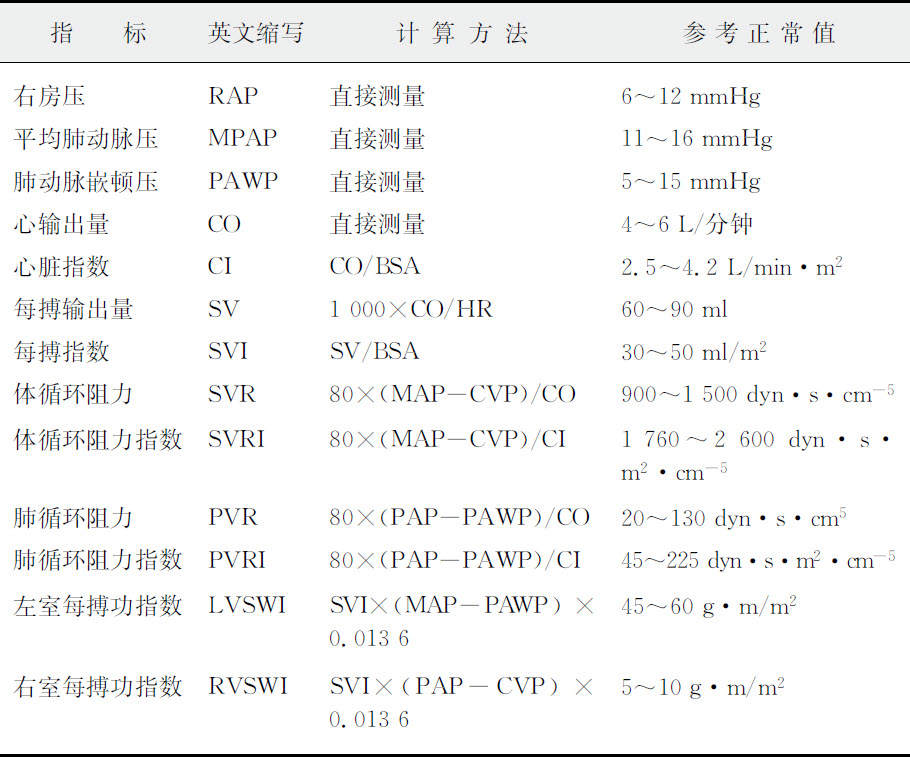
\includegraphics[width=5.89583in,height=2.59375in]{./images/Image00038.jpg}
\end{table}

区别咯血和呕血一般不难,但如患者出血急骤,量多或病史诉说不清时,有时鉴别并不容易;因此须详细询问有关病史,作细致的体格检查,及时作出诊断。

如已明确为咯血,须进一步探索其原因。引起咯血的原因很多(表\ref{tab4-2}),其中最常见的疾病是肺结核、支气管扩张、肺脓肿、支气管肺癌。此外支气管结石、肺寄生虫病、心血管疾病(特别是二尖瓣狭窄)、结缔组织病、钩端螺旋体病等也可引起咯血。

\begin{table}[htbp]
\centering
\caption{引起咯血的常见疾病分类}
\label{tab4-2}
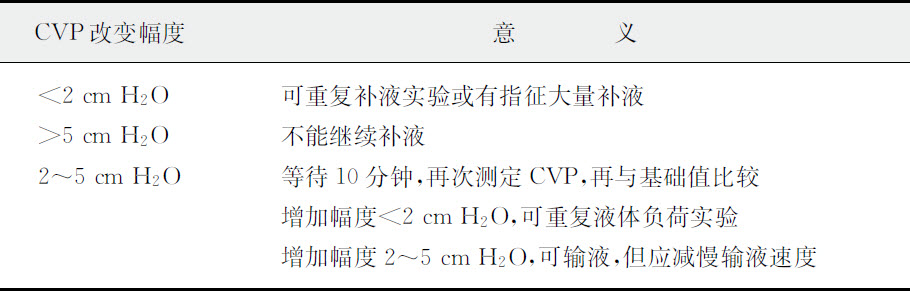
\includegraphics[width=5.89583in,height=4.80208in]{./images/Image00039.jpg}
\end{table}

如咯血量较大,应即采取急救措施,以尽早确定出血的部位。当X线检查的条件未具备时,可应用听诊法以确定。如咯血开始时一侧肺部呼吸音减弱或(及)出现湿啰音,而对侧肺野呼吸音良好,常提示出血即在该侧。气管和支气管疾病所致出血,全身症状一般不严重,胸部X线检查基本正常,或仅有肺纹理增粗;肺部病变所致出血,有比较明显的全身症状,胸部X线检查常发现病变阴影;必须指出,咯血可为全身疾病表现的一部分,临床医生必须对咯血患者做全身检查,以作出正确的诊断。

对于咯血患者,全面分析病史资料常可对咯血原因做出初步估计,同时还需要进一步做下列有关检查:

\subsection{1.病史}

须询问出血为初次或多次。如为多次,与以往有无不同。发生于幼年可见于先天性心脏病;儿童少年慢性咳嗽伴小量咯血和低色素性贫血,须注意特发性肺含铁血黄素沉着症;青壮年咯血多注意肺结核、支气管扩张等疾病;40岁以上有长期大量吸烟史(纸烟20支/
日×20年以上)者,要高度警惕支气管肺癌的可能性;年轻女性反复咯血也要考虑支气管结核和支气管腺瘤。在既往史上需注意幼年是否曾患麻疹、百日咳。在个人史中须注意结核病接触史、多年吸烟史、职业性粉尘接触史、生食螃蟹与蝲蛄史、月经史等。

细致观察咯血的量、颜色,有无带痰。肺结核、支气管扩张、肺脓肿、支气管结核、出血性疾病咯血颜色鲜红;肺炎球菌大叶性肺炎、肺卫氏并殖吸虫病和肺泡出血可见铁锈色血痰;烂桃样血痰为肺卫氏并殖吸虫病最典型的特征;肺阿米巴病可见脓血样痰呈棕褐色,带腥臭味;砖红色胶冻样血痰主要见于克雷伯杆菌肺炎;二尖瓣狭窄肺淤血咯血一般为暗红色;左心衰竭肺水肿时咳浆液性粉红色泡沫样血痰;并发肺梗塞时常咳黏稠暗红色血痰。大量咯血常由于空洞型肺结核、支气管扩张、慢性肺脓肿、动脉瘤破裂等所致;国内文献报告,无黄疸型钩端螺旋体病也有引起致命的大咯血。而痰中带血持续数周或数月应警惕支气管肺癌;慢性支气管炎咳嗽剧烈时可偶有血性痰。

详细询问伴随症状如发热、胸痛、咳嗽、痰量等。咯血伴有急性发热、胸痛常为肺部炎症或急性传染病,如肺出血性钩端螺旋体病、流行性出血热;咯血、发热同时伴咳嗽、咳大量脓痰多见于肺脓肿;长期低热、盗汗、消瘦的咯血应考虑肺结核;反复咳嗽、咳脓痰不伴有发热多见于支气管扩张。

\subsection{2.体格检查}

活动期肺结核和肺癌患者常有明显的体重减轻,而支气管扩张患者虽反复咯血而全身情况往往较好。有些慢性心、肺疾病可伴有杵状指(趾)。锁骨上淋巴结肿大在中老年患者要注意肺内肿瘤的转移。肺部闻及局限性哮鸣音提示支气管有狭窄、阻塞现象,常由肿瘤引起。肺部湿性啰音可能是肺部炎症的体征,也应考虑是否为血液存积在呼吸道所致。对咯血患者还应注意有无全身的出血表现。

\subsection{3.实验室检查}

痰检查有助于发现结核杆菌、真菌、癌细胞、肺吸虫卵等。出血时间、凝血时间、凝血酶原时间、血小板计数等检查,有助于出血性疾病的诊断。外周血红细胞计数与血红蛋白测定可推断出血的程度。外周血中嗜酸性粒细胞增多提示寄生虫病的可能性。

\subsection{4.X线检查}

对于咯血患者,除个别紧急情况不宜搬动外,均应做胸部X线检查。肺实质病变一般都能在X线胸片上显示阴影,从而及时作出诊断。如疑有空洞、肿块,或见肺门、纵隔淋巴结肿大,可加做胸部X线体层摄片或CT检查,CT还有助于发现细小的出血病灶。对疑有支气管扩张者,可做高分辨CT检查等协助诊断。对疑为支气管动脉性出血所致大咯血,必要时可行CT支气管动脉造影(CTA)或数字减影血管成像(DSA)检查,明确出血部位,后者尚可同时进行栓塞介入治疗。

\subsection{5.纤维支气管镜检查}

原因未明的咯血,尤其伴有支气管阻塞者,应考虑纤维支气管镜检查,可发现气管和支气管黏膜的非特异性溃疡、黏膜下层静脉曲张、结核病灶、肿瘤等病变,并可在直视下钳取标本作病理组织检查,吸取分泌物或灌洗液送细菌学和细胞学检查。

\subsection{6.其他检查}

先天性心脏病的诊断往往借助右心导管检查。放射性核素67镓对恶性肿瘤组织较健康组织有更大的亲和力,因而枸橼酸67镓肺部扫描可能有助于肺癌与其他肺部肿物的鉴别诊断。PET/CT对肺部肿瘤引起的咯血的诊断也有帮助。

咯血量的多少视病因和病变性质而不同,但与病变的严重程度并不完全一致,少则痰中带血,多则大口涌出,一次可达数百或上千毫升。临床上常根据患者咯血量的多少,将其分为少量咯血、中量咯血和大量咯血。但界定这三种情况的咯血量多少的标准尚无明确的规定,但一般认为24小时内咯血量少于100ml者为小量咯血;100~500ml/d者为中量咯血;>500ml或一次咯血量>100ml者为大量咯血。

临床上无异常肺部X线征象的咯血病例并不少见,诊断较为困难,其主要原因可能为:①气管或大支气管的非特异性溃疡,一般表现为小量咯血或血痰,支气管镜检查可以发现。②气管或支气管的静脉曲张,多见于右上叶支气管开口处或隆突部分,常引起大咯血,无痰,可经支气管镜检查而发现。③肺动脉瘤、支气管小动脉粥样硬化破裂,肺动静脉瘘破裂。④小块肺栓塞,常不易发现,一般有心脏病、下肢深静脉血栓形成、外伤史、长时间卧床或处于产褥期病史。⑤钩虫蚴、蛔虫蚴、血吸虫毛蚴、比翼线虫在肺内游移引起咯血。⑥早期支气管肿瘤,轻度支气管扩张、支气管结核,肺结核早期等。纤维支气管镜的广泛应用,结合胸部X线检查大大提高咯血病因的确诊率,国内一组917例经胸部X线与纤维支气管镜检查而确定的咯血病因如表\ref{tab4-3}所示:\footnote{*既有临床表现又有X线表现}

\begin{table}[htbp]
\centering
\caption{917例咯血的病因分析(X线诊断与纤支镜诊断比较)}
\label{tab4-3}
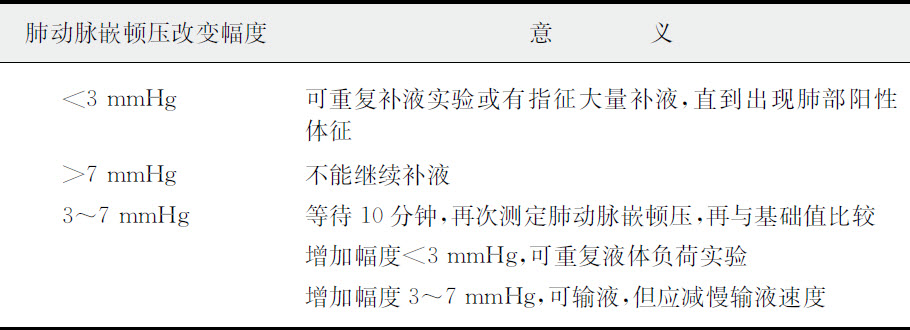
\includegraphics[width=5.91667in,height=3.58333in]{./images/Image00040.jpg}
\end{table}

由表\ref{tab4-3}所示,有部分咯血患者虽经X线和纤维支气管镜检查,仍未能发现阳性结果,且患者亦无引起咯血的全身性疾病,此类咯血可称为特发性咯血。但仍有可能在以后随诊中,在这类“特发性咯血”患者的一部分中,检出呼吸系统疾病。

国内曾有报告一组390例胸片无明显异常的咯血患者,作纤维支气管镜检查,结果发现肺癌16例(4.1\%)、支气管结核2例、支气管腺瘤1例,支气管囊性静脉曲张出血l例。作者认为咯血患者40岁以上,吸烟指数(吸烟年限×每天吸烟支数)>400,咯血时间长,且为痰血而非纯咯血者,尤须警惕肺癌的可能性。

X线胸片是咯血患者的常规检查,但可能无阳性发现。X线胸片正常的咯血患者应进一步作病因学诊断。有作者推荐应先作CT检查,以期发现潜在的肺部病灶,并有助于以后做纤维支气管镜检查时,有目标地进行刷检、活检取材,提高咯血的病因学诊断率。

\protect\hypertarget{text00057.html}{}{}

\subsection{12.1 气管和支气管疾病}

\subsubsection{一、急、慢性支气管炎}

急、慢性支气管炎患者有时也可咯血,一般为小量或痰中带血,不需治疗,可在数天内自行停止,但易于再发。如出血量大,需注意其他原因。本病的咯血与支气管炎症加剧有一定的关系,故咯血前常有病情加重的表现。慢性支气管炎患者发生持续的小量咯血时,须小心寻找其他原因,特别是支气管肺癌。

\subsubsection{二、非结核性支气管扩张}

非结核性支气管扩张可分为原发性与继发性。继发性者是由于支气管内或支气管外阻塞,引起支气管腔与支气管壁的感染,从而损害支气管壁的各层组织所引起。原发性支气管扩张则无明显的引起支气管阻塞的因素,但多数有肺炎病史,特别是麻疹、百日咳、流感等所继发的支气管肺炎史。

咯血是非结核性支气管扩张的常见症状,文献报告约90\%患者有不同程度的咯血,并作为提示诊断的线索。咯血可从童年即开始,常伴有杵状指(趾)。

此病的咯血有两种不同表现:

\paragraph{1.小量咯血}

在经常有慢性咳嗽、脓痰较多情况下,同时有小量咯血;有时在咯血前先有咳嗽较剧烈的一段感染加重阶段。因感染导致支气管内肉芽组织充血及损伤小血管而出现咯血。

\paragraph{2.大咯血}

由于支气管有炎症病变,血管弹性纤维被破坏,管壁厚薄不匀或形成假血管瘤,加上炎症影响,易破裂引起大咯血。咯血量每次达300~500ml以上,色鲜红,常骤然止血(因此类出血常来自支气管动脉系统,压力高,而动脉血管壁弹性好,收缩力强,故可较快止血)。

患者病程虽长,但全身情况尚好。咳嗽和咳痰也为常有的症状,咳嗽可轻微,也可相当剧烈;咳嗽和咳痰常与体位改变有关,如在晨起或卧床后咳嗽可加剧,咳痰增多。痰量可为大量,每天达数百毫升(湿性型)。痰液静置后可分为三层:上层为泡沫状黏液,中层为较清的浆液,下层为脓液及细胞碎屑沉渣。有些患者痰量甚少(干性型),如合并感染,痰量随之增多,并有发热、咯血等。

支气管扩张的好发部位是下肺,以左下叶较右下叶为多见,最多累及下叶基底段,病灶可延伸至肺边缘。病变部位出现呼吸音减弱和湿性啰音,位置相当固定,体征所在的范围常能提示病变范围的大小。

胸部X线平片检查不易确诊本病。国内一组84例非结核性支气管扩张中,只1/3病例在胸部X线平片上有少许的征象,大部分甚至没有任何改变。胸部X线平片检查对排除慢性肺脓肿及慢性纤维空洞型肺结核颇有帮助。如患者有支气管扩张的临床表现,X线胸片又显示一侧或双侧下肺纹理增粗、紊乱以及蜂窝状小透亮区,或见有液平面则支气管扩张的可能性最大,胸部CT检查可确定诊断,并对明确病变部位及决定治疗方案有重要意义。

全内脏转位、支气管扩张、鼻窦病变三联症,又称Kartagener综合征,国内有少数病例报告。此综合征有咳嗽、咳痰、咯血等症状。咯血可从童年开始,反复发作,量不多。

\subsubsection{三、结核性支气管扩张}

结核性支气管扩张的症状因肺内结核病灶的情况而定,如肺结核病灶不严重,则可无明显症状。有时或可闻及少许干、湿性啰音。X线胸片上显示病灶似已硬结,而患者仍有或多或少的咯血,应考虑结核性支气管扩张的可能性。国内一组64例患者中,发病大多在30岁以上,90\%有咯血(痰中带血或大量咯血)。病灶部位大都在两肺上叶,尤以右上叶的后段、左上叶的尖后段多见。

结核性支气管扩张与非结核性支气管扩张的鉴别见表\ref{tab4-4}。

\subsubsection{四、支气管结核}

支气管结核一般为继发性,原发性者罕见。患者大多有咯血,其他常见症状为阵发性剧烈咳嗽、喘鸣、阵发性呼吸困难等。有时轻度动作即可引起呼吸困难与发绀。如发生支气管阻塞,则引起突然的发热、痰量减少,而阻塞解除后痰量突然增加,体温也下降。

\begin{table}[htbp]
\centering
\caption{结核性与非结核性支气管扩张的鉴别要点}
\label{tab4-4}
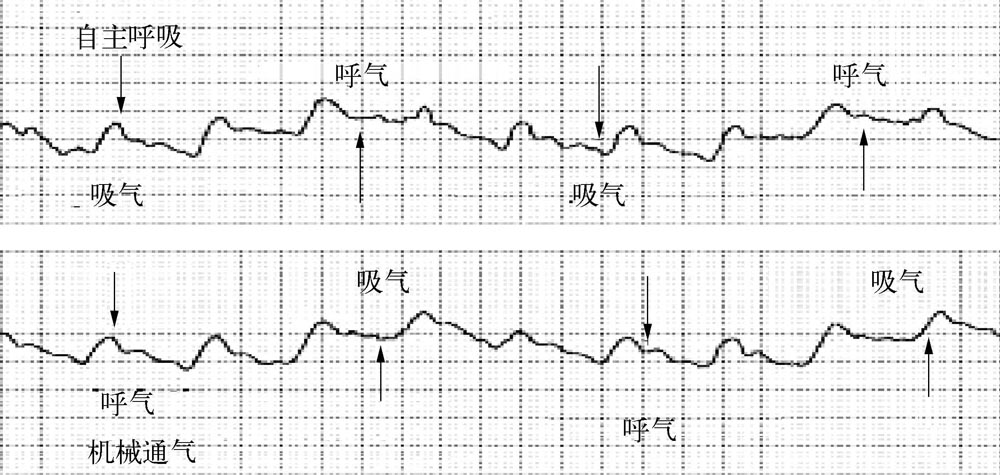
\includegraphics[width=5.94792in,height=1.65625in]{./images/Image00041.jpg}
\end{table}

支气管结核是发生于气管、支气管黏膜或黏膜下层的结核病变。据国内报告,肺结核合并支气管结核者占23.6\%~57.1\%。患者以青壮年为多,文献报告女性罹患多于男性,常发生于慢性纤维空洞型肺结核、慢性血行播散型肺结核、支气管淋巴结结核、浸润型肺结核及干酪样肺炎等基础之上。这些患者有下列情况提示有支气管结核的可能:①反复小量咯血或血痰而X线胸片未见明显病变者;②药物难以控制的刺激性咳嗽;③有喘鸣音;④有不同程度的呼吸困难而不能用肺实质病变解释者;⑤肺无明显病变而痰结核菌屡为阳性;⑥肺内有新播散病灶而不能用其他原因解释;⑦肺结核并发肺不张;⑧某些肺野空洞:在萎陷疗法后产生的张力性空洞;空洞时大时小;出现圆形、薄壁空洞;肺门附近的空洞等。

支气管结核的确诊须依靠纤维支气管镜检查。如临床症状典型,虽纤维支气管镜检查阴性,也不能除外此病的存在。

近年国内一组单纯气管、支气管结核病28例报道,误诊颇多,原因为:①胸片无异常发现;②胸片虽出现局限性肺气肿、肺纹理密集、肺纹理粗乱、叶间胸膜影移位等异常表现,但又非特异性而未加注意。作者建议对干咳、胸闷、喘息、咳黏液痰或咯血患者,经抗感染及对症治疗2周未见好转时.应及早作纤维支气管镜检查,镜下刷检涂片染色找抗酸杆菌,或钳取组织做病理检查。镜下所见仍疑似结核而实验室检查阴性时,2周后应再做纤维支气管镜检查。

目前将刷检标本或支气管肺泡灌洗液进行PCR检测结核分枝杆菌,可大大提高病原学诊断率。

结核感染T细胞斑点(T-SPOT.TB)试验是近年来的一项新诊断技术,通过检测外周血分泌γ-干扰素的T淋巴细胞数量来诊断结核感染,具有较高的特异性和敏感性,且不受卡介苗接种和环境分枝杆菌感染的影响,在肺结核的筛查和诊断中有较好的应用价值。

\subsubsection{五、支气管结石}

本病的特点为反复咯血,而肺部除有钙盐沉积之外,无其他原因可解释。患者或曾有咳出结石史。咯血通常为小量,但有些患者可有大咯血。X线检查发现有支气管结石阴影,以右中叶根部较为多见,结石远端可发现有阻塞性肺不张或肺部感染,CT检查可见支气管阻塞远端有钙化影。纤维支气管镜检查可帮助诊断。支气管结石常由肺结核病灶钙化引起。X线胸片上如炎症病变相应部位有钙化结节,在炎症消退后而咯血不断者,则支气管结石的可能性甚大。

据国内一组20例的报告中,以咯血为主要症状者占95\%,其中威胁生命的大咯血占40\%。误诊率60\%。并发症(占85\%)表现为肺不张、支气管扩张、阻塞性肺炎等。但手术治疗效果好。X线断层摄片、胸部CT和纤维支气管镜检查等综合检查对诊断有较大帮助。

\subsubsection{六、原发性支气管肺癌(肺癌)}

本病大多见于40岁以上男性,文献报告有咯血者占50\%~70\%,国内一组141例报告中,第一个月内出现咯血者有38.3\%。中央型肺癌较周围型肺癌易引起咯血。癌组织内小血管较多,患者又常有刺激性咳嗽,易引起癌组织损伤而致出血。其特点是痰中带血或小量咯血多见,而大量咯血少见,但晚期可有致命性大咯血。咳嗽是较常见的早期症状,无痰或有少量的白色黏液痰,可伴有胸痛。间断的或持续的小量咯血,对提示此病的诊断有重要意义。痰中可混有小颗粒状灰白色坏死组织,其中较易找到癌细胞。X线胸片、纤维支气管镜、胸部CT及活组织病理检查有助于诊断。

国内一组确诊肺癌患者1105例中,纤维支气管镜下直接见到肿瘤病灶(直接征象)者638例(57.7\%),只见肿瘤间接征象,即支气管黏膜改变者412例(37.3\%)。肺癌多见于段以上的支气管(中央型肺癌约占3/4),有些病例第一次活检及刷检均未能确诊,需做第二次,偶尔还要第3~4次检查。当发现有间接征象的可疑病例,应尽可能多部位活检多取标本,甚至看到癌体也应多点活检。

\subsubsection{七、支气管类癌}

支气管类癌罹患多为中年人,男女性别无差异,生长慢,具有恶性程度低和较少发生转移的特点。早期症状常为咯血,术后长期生存率较高。国内一组17例报告中,患者40岁以下者占64.7\%,中央型12例,周围型5例,2例有支气管旁淋巴结转移,主要临床表现为咳嗽、咳痰、咯血或痰中带血、发热和反复发作肺部炎症。临床上本病易误诊为肺癌、结核球或良性支气管肿瘤。X线检查与纤维支气管镜下活检对诊断帮助较大。

\subsubsection{八、良性支气管瘤}

良性支气管瘤少见,发病多在30~40岁之间。全身情况良好的中年患者如有反复的小量咯血或痰中带血,或类似哮喘发作,或屡次发作的呼吸道阻塞及感染症状,应考虑此病的可能。由于肿瘤生长缓慢,临床症状可延续多年。早期可无症状,或仅有气喘、干咳,有时甚至被误诊为支气管哮喘。肿瘤逐渐增大而堵塞支气管时,可发生相应肺叶的肺不张,并在肿瘤的远侧发生感染与支气管扩张。X线体层摄片、胸部CT,可了解较大的支气管内肿瘤的范围及部位,气道阻塞情况及继发性支气管扩张,对诊断有重要帮助。由于良性瘤多发生于较大的支气管内,纤维支气管镜检查的检出率可达85\%~90\%。

良性支气管瘤有腺瘤、平滑肌瘤、乳头状瘤等,此外较罕见的有纤维瘤、软骨瘤、脂肪瘤等。其中腺瘤比较多见,典型X线征象为肺门附近有圆形或类圆形阴影,密度均匀一致,边缘锐利,体层摄片或胸部CT检查更易于发现;由于多数腺瘤位于主支气管或肺叶支气管内,纤维支气管镜检查易作出诊断。

\protect\hypertarget{text00058.html}{}{}

\subsection{12.2 肺部疾病}

\subsubsection{一、肺结核}

咯血是肺结核患者常见的症状,且常为提示此病诊断的线索。咯血量多寡不一,少可仅为痰中带血,多则一次可达500ml以上,血色鲜红。咯血与结核病变的类型有一定关系,多见于浸润型肺结核、慢性纤维空洞型肺结核、干酪样肺炎,而少见于原发综合征(原发型肺结核)和急性血行播散型肺结核。咯血严重程度并不一定与病灶大小成正比,小的病灶可有较多的咯血,而病灶广泛的也可无咯血。出血量常和血管损害程度有关,血管壁渗透性增高所致的咯血,出血量少,但持续时间较长;小血管的破裂则多引起小量出血,这往往由于慢性活动性肺结核所致;大咯血多为肺动脉分支破损所致,其中以空洞内形成的动脉瘤破裂所致的大咯血多见,此类出血来势甚急,而由于洞壁纤维化不易收缩止血,或血凝块虽能填塞空洞压迫血管暂时止血,但又可因血块溶解而再次出血。

肺结核患者以青壮年占大多数,不少患者以咯血为初发症状而就诊。咯血之后常有发热,是由于病灶播散及病情发展所致。患者常同时出现疲乏、纳差、体重减轻、午后潮热、盗汗、脉快和心悸等全身中毒症状。

肺结核的诊断主要依靠症状、体征、X线胸片和痰结核菌检查。如在青壮年人一侧肺尖部经常听到湿性啰音,又有上述全身性中毒症状,则支持活动性肺结核的诊断。X线胸片是诊断肺结核的重要方法,可以发现早期轻微的结核病变,确定病灶的范围、部位、形态、密度、与周围组织的关系,判断病变的性质、有无活动性、有无空洞、空洞大小和洞壁特点等。因此,定期进行胸部X线检查能及早发现病灶,有助于早期治疗。

痰结核菌检查阳性可确诊为肺结核,且可肯定病灶为活动性。但痰结核菌阴性并不能否定肺结核的存在,对可疑病例需反复多次痰液涂片检查,如有需要,可采用浓集法、培养法、PCR法等,在咯血前后,因常有干酪性坏死物脱落,此时的痰菌阳性率较高。

长期被误诊为肺结核咯血的肺部疾病并非少见,文献报道有支气管扩张、支气管囊肿、肺癌、肺脓肿、肺吸虫病等。

年轻患者反复咯血,痰结核菌检查阴性,全身情况较好,而病灶又处于中、下肺野,用一般抗菌药物治疗能改善炎症表现者,则可认为是非结核性支气管扩张,胸部CT检查有助于确定诊断。支气管囊肿在胸部平片及透视下一般可确定诊断。非结核性支气管扩张或支气管囊肿合并普通细菌感染时,其症状的出现通常较早,可追溯到童年时期,特别是在患麻疹、百日咳之后常有咯血及呼吸道炎症症状,其与肺结核病的鉴别是前两者在长期的病患过程中,全身一般状况仍较好,无结核病的全身中毒症状,可伴有杵状指(趾),痰结核菌阴性。

肺癌被误诊为肺结核者颇为常见。在下列情况下,应考虑肺癌的可能:①年龄在40岁以上,尤其是长期重度吸烟的男性患者,新近出现反复的咯血或持续的痰中带血,或近肺门处有致密的异常阴影,或出现肺不张合并感染,而多次痰液检查未发现结核菌者,应首先考虑肺癌的可能;但痰中结核菌阳性也不能除外肺结核与肺癌并存。②肺癌组织内部发生坏死破溃,坏死组织排出后形成空洞,其X线征象可酷似结核性空洞。但癌性空洞常呈偏心性,其内侧壁凹凸不平,外缘多呈毛刺状、分叶状,常无病灶周围卫星灶,多次痰结核菌检查阴性,经规律的抗结核治疗无效,病灶逐渐增大,这些均可与肺结核鉴别。③肺癌和肺结核并存,肺癌可发生在陈旧性肺结核瘢痕的基础上,而肺癌又能促使结核病灶恶化。如在陈旧性或活动性结核病灶处出现新的、致密的圆形病灶,且经积极抗结核治疗一个月后,病灶仍逐渐增大,或出现肺不张、肺门阴影增大,癌性空洞等改变,应考虑并存肺癌的可能。

\subsubsection{二、肺 炎}

在急性肺炎时,肺实质处于高度充血状态,小血管通透性增加并可发生破裂而致咯血。由于小血管可发生血栓性脉管炎,致血管腔闭塞,通常不易引起大量咯血。

肺炎链球菌肺炎的患者,痰中混有血液者并不少见,有时血量可达20~30ml,病期第2、3天转为铁锈色痰。在整个病程中均呈血性痰的甚少。

肺炎杆菌性肺炎多为砖红色稠胶样痰;化脓性链球菌肺炎咳粉红色稀痰;葡萄球菌肺炎可为血性痰、脓性痰;绿脓杆菌肺炎咯血少见,典型者咳翠绿色脓痰。军团菌肺炎少量黏液痰中可带血丝,并有发热、咳嗽、肌痛、关节痛、腹泻、蛋白尿、转氨酶升高、直接荧光抗体阳性或间接荧光抗体1∶256。肺炎支原体肺炎约1/4病例有血性痰,但绝无铁锈色痰;流感病毒性肺炎常引起反复的小量咯血。

\subsubsection{三、肺脓肿}

肺脓肿多由于吸入感染或血源性感染所引起,约50\%患者伴有咯血,常伴有大量脓痰或脓血样痰。急性肺脓肿的早期可有大量的咯血而无脓痰,但此时有寒战、高热、胸痛、血白细胞和中性粒细胞增高,提示急性细菌性感染,1周后可出现大量脓性痰。慢性肺脓肿常有大量的脓痰或脓血痰,痰量每天可达300~500ml,带臭味,痰静置分层,多数患者伴有杵状指。慢性肺脓肿常被误诊为肺结核病,前者可根据急性发病史、X线胸片见大片浓密模糊浸润阴影,脓腔内出现圆形透亮区及气液平面,痰培养可有致病菌生长以及抗菌治疗有效,一般鉴别不难。慢性肺脓肿与肺癌的区别,可根据肺脓肿过去的急性发病史、空洞的特点及痰中癌细胞检查等加以鉴别,X线胸片、纤维支气管镜、胸部CT扫描有利于诊断。癌性空洞与肺脓肿空洞、结核性空洞的鉴别参见表\ref{tab4-5}。

\begin{table}[htbp]
\centering
\caption{癌性空洞与肺脓肿空洞、结核性空洞的鉴别}
\label{tab4-5}
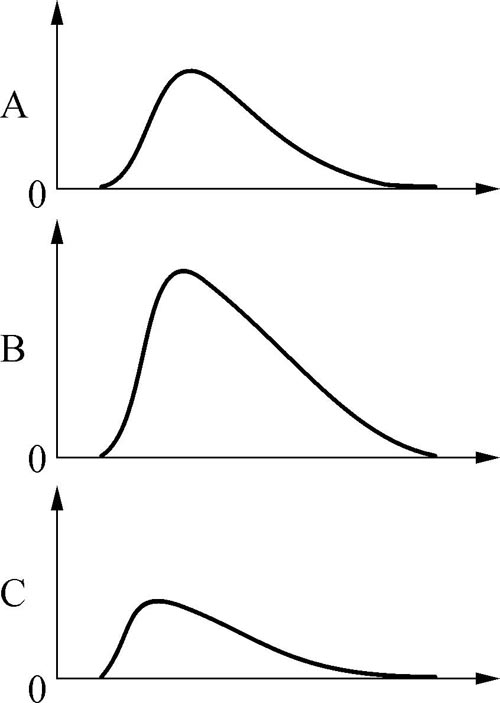
\includegraphics[width=5.97917in,height=3.53125in]{./images/Image00042.jpg}
\end{table}

\subsubsection{四、肺部真菌感染}

肺部真菌感染是最常见的深部真菌病,主要由念珠菌、曲霉、毛霉、新型隐球菌等真菌感染所致。老年、幼儿及体弱者易患此病,多为痰中带血或小量咯血。常见症状有发热、乏力、盗汗、纳差、消瘦、咳嗽、胸痛;痰的特点是量少,不同种类的真菌感染时,其痰的性状不一。肺白念珠菌感染,为胶样黏稠痰,带乳块或血丝;肺曲霉病反复咯血或咳出大量泡沫痰(可带酒味);肺新型隐球菌病则咳小量黏液性痰或血丝痰。病原学检查可找到致病菌,胸部X线检查,肺组织病理检查有助于诊断。

\subsubsection{五、肺寄生虫病}

\paragraph{1.肺阿米巴病}

阿米巴性肺脓肿为肝阿米巴病并发症之一,也可来自肠道病灶。多数起病较慢,常有发热、乏力、消瘦、咳嗽、咳痰、右下胸痛并放射至右肩,少数呈急性发病,高热、胸痛、呼吸困难等,可有肝脏肿大体征。典型的痰液呈棕褐色而带腥臭味,有助于此病的诊断。如合并出血或混合感染,可呈血性或黏液脓血痰。痰液、胸腔积液或纤维支气管镜取病变坏死组织中查找到溶组织阿米巴滋养体可确诊。

\paragraph{2.肺吸虫病}

本病有严格的地区性,患者都曾有在疫区进食未煮熟的含有肺吸虫囊蚴的石蟹或蝲蛄史。病程中常反复的小量咯血,痰血混合多呈特殊的棕黄色或铁锈色,烂桃样血痰是肺吸虫病最典型特征。早期症状有畏寒、发热、脐周隐痛、腹泻,并有乏力、盗汗、纳差,2~3周后出现咳嗽、胸痛、咯血等,患者虽有长期的反复咯血,但全身情况尚好,胸部体征多不明显,可有皮下结节。常有血嗜酸性粒细胞增多,痰中发现肺吸虫卵即能确诊,阳性率90\%以上。粪便虫卵检查、肺组织病理检查、免疫学检查、X线检查等有助于诊断。

胸部X线检查有较特别的征象,病灶多位于中、下肺野及内侧带,因病变的不同时期而有下列的表现:①早期呈边缘模糊的弥漫阴影,大小约为1~2cm;②中间期为边缘清楚、多房或单房的、实质或囊状的大小不等的阴影,多房性囊状阴影是本病的X线特征;③晚期为纤维增殖性变及硬结钙化阴影。此外,可有肺门增大、肺纹理增粗紊乱、胸腔积液或胸膜增厚等征象。对一些疑难的、不典型的病例,流行病学调查和免疫学检查,在诊断上有重要意义。

如患者有上述的流行病学史和胸痛、咳铁锈色痰等症状,血嗜酸性粒细胞增多,痰中虽未发现肺吸虫卵,而肺吸虫抗原皮内试验阳性,并已除外血吸虫病、华支睾吸虫等感染时,则大致可作出肺吸虫病的临床诊断,并应进行特效药物(如吡喹酮)的诊断性治疗;如疗效显著,可进一步确立诊断。肺吸虫病主要须与肺结核相鉴别(表\ref{tab4-6})。

\begin{table}[htbp]
\centering
\caption{肺吸虫病与肺结核鉴别}
\label{tab4-6}
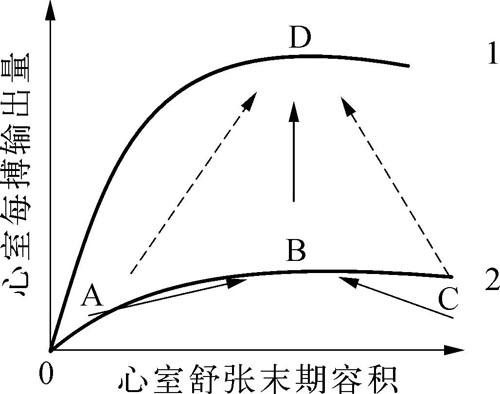
\includegraphics[width=5.94792in,height=4.91667in]{./images/Image00043.jpg}
\end{table}

在四川及福建发现的肺吸虫病,临床表现较特别,其症状轻,咯血量较小,痰中虫卵检出率较低,有游走性皮下结节者甚多(多分布于胸壁及上腹壁),血中嗜酸性粒细胞显著增多。

国内报道肺吸虫病误诊率较高。主要原因是由于肺吸虫病临床表现及X线胸片大多无特异性,且典型的游走性皮下结节,肺空泡、结节和隧道线条等X线表现又少见。一组报道34例肺吸虫病在入院前全部误诊为肺结核。

由于肺吸虫病免疫学诊断的敏感性和特异性高,且简便易行,在流行区内患者有生食石蟹或蝲蛄史,而反复出现咳嗽、咯血或痰中带血、发热等症状,应即作肺吸虫抗原皮内试验,上述一组误诊为肺结核的34例患者,肺吸虫抗原皮内试验全部为1∶2000以上阳性。应用混合单抗双抗体夹心ELISA法诊断疑难肺吸虫病,效果更佳。

\paragraph{3.肺包虫病}

肺包虫病是棘球绦虫的幼虫(棘球蚴)寄生于人体肺内所引起,主要流行于畜牧区,以青壮年农民和牧民为主,早期可无症状。当包囊肿大破裂时可出现咯血或痰中带血,并可咳出类似粉皮样的角皮膜;合并感染时则出现咳嗽、咳痰、胸部不适,或胸痛及劳力后气促等症状。可有肝脏或其他部位囊肿征象。囊肿破裂,囊液亦可阻塞气管而引起窒息。X线胸片或CT扫描有助于诊断,可显示包虫圆形或卵圆形,略呈分叶状阴影,边缘清晰,密度均匀,壁可钙化,阴影随呼吸而变形;包虫囊壁破裂,空气进入,则顶部呈现半月形透亮带。包虫抗原皮内试验及补体结合试验对本病有重要的诊断意义,阳性率可达90\%以上。此外,痰检查、B超检查、放射性核素扫描等对诊断也有帮助。

\subsubsection{六、恶性肿瘤的肺转移}

恶性肿瘤转移至肺部时,可引起咯血。较常发生肺部转移的恶性肿瘤有鼻咽癌、乳腺癌、食管癌、胃癌、肝癌、结肠直肠癌、前列腺癌、睾丸畸胎瘤、精原细胞瘤、绒毛膜上皮细胞癌、恶性葡萄胎及类癌等。以绒毛膜上皮细胞癌、睾丸畸胎瘤和恶性葡萄胎的肺转移的咯血发生率最高。对成年女性原因未明的咯血,患者阴道曾排出水泡样胎块,或兼有流产后持续的不规则阴道出血,应考虑恶性葡萄胎或绒毛膜上皮细胞癌的可能性,尿妊娠诊断试验有助于此病的诊断。

转移性肺恶性肿瘤常为多发,但也可为单发,后者较少见。X线胸片显示多发性肺转移肿瘤的形态多为圆形、卵圆形或粟粒状阴影,大小相仿,边缘不整,发展较快。转移性肺恶性肿瘤原发病灶的诊断有时不易,须设法寻找。

\subsubsection{七、肺梅毒}

本病极为少见,国内仅有二例感染报告,均有咯血。病程进展缓慢,往往有咳嗽、咯血、胸痛等症状,虽然X线胸片显示下肺野呈大片状实质模糊阴影,但全身情况良好。诊断须依据梅毒感染史、梅毒血清反应阳性与驱梅治疗的疗效。肺梅毒须与其他肺部疾病相鉴别,特别是肺结核病。

\subsubsection{八、肺囊肿}

肺囊肿可区分为先天性与后天性两类,以前者较为多见,后者是由肺部感染性疾病或寄生虫所引起。多发性先天性肺囊肿常伴有支气管扩张,多在儿童期出现症状,其临床表现与支气管扩张相似,患者往往因突然小量咯血或痰中带血而就诊,由于病变多位于中、上肺,引流较好,较少出现发热。X线胸片检查呈圆形透亮影,其壁菲薄而整齐;多发者大小不一,可分布于任何肺野,但以中、上肺野较多见。

多发性先天性肺囊肿需与支气管扩张鉴别。肺囊肿继发感染时可出现大片状模糊阴影,类似浸润性肺结核,但经抗生素治疗后感染较快消退,而有别于肺结核。肺囊肿合并感染时,其临床症状和X线胸片的改变与肺脓肿相似,需加以鉴别。

国内曾报告一组82例的成年患者中,52例(63.4\%)有咯血,多数在200ml以下,认为如有下列情况应考虑本病:①肺部阴影长期存在;②阴影在同一部位反复出现;③无播散灶;④阴影新旧程度一致;⑤肺门及纵隔淋巴结不大。患者虽反复咯血而无结核中毒症状。胸部CT检查有助于对本病的诊断。

近年肺囊肿有一组38例报告,发病常在青少年期,5例初发年龄在10岁以下。全部患者(38例)在院外均被误诊为肺结核。初发症状以咯血或痰中带血多见(21/38),咳嗽、咳痰、发热次之。6例无症状患者经体检而发现本病。21例有长期反复出现咯血或痰中带血史,最长者达20年。

肺囊肿的胸部X线表现常缺乏特征性。作者认为以下几点有利于肺囊肿的早期诊断:①发病年龄在30岁以下,特别是男性,有反复咯血或痰中带血、咳嗽、发热史。②动态观察X线胸片阴影的形态变化不大,无肿瘤的淋巴结、淋巴道远处转移的改变。③结核菌素试验阴性或经积极的抗结核治疗无效。④胸部X线显示其病变虽无固定部位但与支气管走向有关;虽经反复感染但病变部位固定不变;在非囊肿部位不出现新的病灶。⑤有条件时应作高分辨胸部CT检查加以鉴别。⑥经上述不能确诊时应考虑肺活检或外科手术探查。

\subsubsection{九、尘 肺}

包括硅沉着病和其他尘肺,是由于长期吸入某种粉尘所致的以肺实质弥漫性纤维病变为主的疾病。主要发生于从事粉尘作业的工人,可有慢性、顽固性咳嗽,咳泡沫状痰、咯血或痰中带血,气短和胸痛。早期症状不明显,常为干咳或带黏稠痰,晚期咳嗽加重,痰多,如合并肺结核或支气管扩张,可反复大咯血。晚期病情重,有发绀、杵状指、肺气肿、肺源性心脏病等表现。胸片可见中、下肺野呈网状、条索状或结节状阴影改变,肺门淋巴结肿大。其诊断主要依据为职业病史、临床表现、胸部X线征象及肺功能检查。

硅沉着病合并肺结核比无硅沉着病的发病率高4~5倍,其特点是肺结核的发生率和严重程度与硅沉着病的发展程度成正比,硅沉着病愈严重,其并发肺结核的可能性愈大,肺结核病的病变发展也愈迅速,病情愈严重。石棉肺合并肺结核比较少见,但合并肺癌者却较多。

\protect\hypertarget{text00059.html}{}{}

\subsection{12.3 肺血管及其他循环系统疾病}

\subsubsection{一、肺血栓栓塞症}

肺血栓栓塞症是肺栓塞的最常见类型,占肺栓塞中的绝大多数,多继发于右心或体循环深静脉系统的血栓形成,偶尔也见于肺动脉炎、感染性心内膜炎等病例中,是以各种栓子阻塞肺动脉系统为其发病原因的一组疾病或临床综合征。主要症状为呼吸困难及气促、胸痛、小量咯血(大咯血少见)、咳嗽、心悸、发热等。心瓣膜病(特别是合并心房颤动)患者发生咯血、未能解释的短期发热时,须考虑肺血栓栓塞症的可能。X线胸片可显示区域性肺纹理变细、稀疏或消失,肺野透亮度增加;也可显示肺组织的继发改变,如肺野局部的片状阴影,尖端指向肺门的楔形阴影,肺不张或膨胀不全,有肺不张侧可见横膈抬高。X线胸片对鉴别其他胸部疾病有重要帮助。螺旋CT、放射性核素肺通气/血流灌注扫描、磁共振显像(MRI)及肺动脉造影都是肺血栓栓塞症的重要确诊方法。

\subsubsection{二、肺动脉高压}

肺动脉高压可由许多心、肺和肺血管疾病引起,根据发病的原因是否明确,曾被习惯性分为“原发性”和“继发性”肺动脉高压。2008年世界卫生组织第4届肺动脉高压会议重新修订了肺动脉高压分类,目前按照病因或发病机制、病理与病理生理学特点分为五个大类:①动脉性肺动脉高压;②左心疾病所致肺动脉高压;③肺部疾病及(或)低氧所致肺动脉高压;④慢性血栓栓塞性肺动脉高压;⑤未明多因素机制所致肺动脉高压。继发性肺动脉高压较原发性肺动脉高压常见,早期临床表现以基础疾病如慢性支气管炎、COPD等的临床表现为主,晚期以右心功能不全的表现为主。原发性肺动脉高压是一少见病,被世界卫生组织改称为“特发性肺动脉高压”,是一种不明原因的肺动脉高压。早期通常无症状,仅在剧烈活动时感到不适;随着肺动脉压力的增高,可逐渐出现呼吸困难、胸痛、头晕或晕厥、咯血。咯血量通常较少,有时也可因大咯血而死亡。其他症状还包括疲乏、无力,雷诺现象,声嘶(Ortner综合征)等。胸部X线检查、超声心动图和多普勒超声检查、放射性核素肺通气/灌注扫描、右心导管术、肺活检都对诊断有重要的作用。

\subsubsection{三、肺动静脉瘘}

肺动静脉瘘是先天性肺血管的血管瘤样畸形,也可为获得性,临床上少见。可有咳嗽、间歇小量咯血、发绀、杵状指(趾)及红细胞增多症。体格检查可发现在相应胸壁部位触及震颤,闻及来回性血管杂音。X线胸片和胸部CT在诊断上起重要作用,可见边缘整齐、密度均匀的圆形或卵圆形阴影,多位于中下肺野,且与肺门之间有条索状阴影,病变无钙化,无空洞形成。肺动静脉瘘发病常与遗传性出血性毛细血管扩张症有关,可误诊为肺结核球或支气管肺癌,肺动脉造影可协助明确诊断。

\subsubsection{四、单侧肺动脉发育不全}

本病少见,患者大多有不同程度的咳嗽、咳痰、痰中带血、胸痛、气促等表现,体格检查可发现患侧胸廓扩张稍受限、语颤及呼吸音减弱、多可听到干、湿性啰音,可被误诊为肺气肿、气胸、支气管扩张等。诊断主要依靠胸部X线检查,尤其是胸部CT的肺动脉造影对诊断极有帮助。

\subsubsection{五、肺淤血}

常见于风湿性心脏病二尖瓣狭窄,且多发生在较严重的瓣口狭窄的慢性充血期,也可见于急性左心衰、复张后肺水肿、高原性肺水肿等,多表现为痰带血丝、小量咯血或咳出粉红色泡沫样痰。结合心脏病史、胸腔快速抽液(气)及快速登山等病史,心尖部舒张期隆隆样杂音,超声心动图和多普勒超声检查等可作出诊断。二尖瓣关闭不全较少引起咯血。

\subsubsection{六、高血压}

在恶性或急进型高血压,由于血压持续增高时,可引起肺毛细血管破裂而出现咯血。也可由于并发急性肺水肿而咳粉红色泡沫样痰。

\subsubsection{七、先天性心脏病}

某些有血液分流的先天性心血管病如房间隔缺损、室间隔缺损、艾森曼格综合征等,均可伴有显著的肺动脉高压,由此可引起咯血。

\protect\hypertarget{text00060.html}{}{}

\subsection{12.4 全身性疾病及其他原因}

\subsubsection{一、急性传染病}

1.肺出血型钩端螺旋体病
肺出血型钩端螺旋体病也称钩端螺旋体性出血性肺炎,是钩端螺旋体病的严重类型,如不注意常易误诊。钩端螺旋体病以夏秋季多发,以青壮年为主,从事牧、渔业劳动者发病率高,大多起病急骤,症状主要有畏寒或寒战、高热、头痛、全身肌肉酸痛、衰弱无力、眼结膜充血、腓肠肌疼痛、淋巴结肿大,多在毒血症过程中出现心悸、烦躁、呼吸和心律逐渐增快。初为痰中带血,以后咯血量增多。严重的肺弥漫性出血型者,可引起致命的大咯血,其特点是发生突然、发展迅猛,临终时多数患者出现从口鼻涌出大量血液,立即窒息而死。X线胸片和胸部CT显示双侧肺野斑片状模糊阴影,以中、下肺野尤其显著。需与其他原因的肺炎、肺结核鉴别。病原学和血清学检查有助于明确诊断。

2.流行性出血热
由汉坦病毒引起,经呼吸道、消化道、母婴、虫媒及动物源传播,流行季节以3~5月份或5~7月份以及11月份至次年1月份间为高峰,青壮年多见,主要损害全身小动脉和毛细血管。患者起病急,典型病例具有发热、出血与肾损害三大主要特征以及发热期、低血压休克期、少尿期、多尿期和恢复期五期经过。其主要临床表现为发热、头痛、腰痛、眼眶痛、口渴、呕吐、酒醉貌、球结膜充血水肿,皮肤和黏膜广泛出血、鼻出血、咯血、呕血、便血、血尿,软腭及腋下有出血点,肾区有叩击痛。早期外周血白细胞正常或偏低,有尿蛋白,尿红、白细胞及管型改变;肾功能损害,约有半数出现肝功能损害。特异性血清学试验有助于确诊。

\subsubsection{二、血液病}

某些血液病如血小板减少性紫癜、白血病、再生障碍性贫血、血友病等均可出现咯血,与原发病有关。除咯血外,尚伴有其他部位的出血倾向。血常规、骨髓细胞学检查、血小板功能与凝血因子检查可确诊。

\subsubsection{三、白塞病(Behcet disease)}

本病由病毒感染、遗传因素、免疫功能及体内微量元素异常等因素引起。初发年龄主要是16~40岁的青壮年,以女性多见。基本病变是血管炎,可累及毛细血管和细小动静脉,可因肺部血管受累而反复咯血,多为小量咯血,也有因肺脉管炎而引起多发性肺栓塞。主要的临床表现为反复发作的口腔黏膜、舌尖及其边缘、齿龈、上下唇内侧等处的痛性小溃疡;外生殖器损害与口腔基本相似;眼部损害主要为结膜炎、角膜炎、虹膜炎、视网膜炎,其他表现有皮肤损害、消化道损害、关节损害及神经系统损害等。活动期多有血沉、黏蛋白、唾液酸、α2球蛋白增高,部分患者血浆铜蓝蛋白及冷球蛋白阳性。本病并发肺脉管炎引起咯血时的胸部X线表现,可类似肺炎支原体肺炎、肺部转移癌,或出现大片密度增高的圆形阴影。病理学检查及有关脏器病变的相应检查有助于诊断。针刺反应阳性是一特征性表现,若能同时检查HLA-B5,对本病的诊断更有帮助。

\subsubsection{四、结缔组织病}

该类疾病如系统性红斑狼疮、结节性多动脉炎、重叠综合征等,其发病与遗传、某些药物、物理因素、病毒感染、内分泌因素、免疫异常等有关,多见于20~40岁的女性。可有小量咯血,如伴有肺动脉受侵害,可发生大咯血。若患者有多个器官系统功能的损害,胸部X线检查见肺部有阴影,而抗菌药物治疗效果不佳时,应考虑结缔组织病伴有肺部损害的可能性。诊断结缔组织病所致的咯血时,须认真除外肺结核、支气管扩张、肺肿瘤等疾病。实验室检查和肺组织病理检查有助于诊断。

\subsubsection{五、肺出血-肾炎综合征}

国外文献曾有多例重度肺出血合并肾小球性肾炎报告,并命名为Goodpasture综合征,病因未明,也有将此病归入结缔组织病,临床上少见。此病多见于20~40岁男性,病程数月至数年,预后不良。临床经过可分为两个阶段:①肺部病变阶段,87\%~96\%以上的病例的首发症状表现为间歇的咯血,轻者为血痰,重者出现大咯血,反复出血可致贫血;病变广泛者可有呼吸困难、发绀与胸痛,X线胸片上显示短暂的弥漫性细小或大片状阴影,但X线检查也可呈阴性。②肾脏病变阶段:多数患者在咯血后数周或数月出现肾炎症状,肾脏病变表现为肾小球性肾炎,起病隐袭,当肺部病变显著时,尿检查发现蛋白尿、镜下血尿与管型尿,早期肾功能正常,当肾脏病变为进行性,尿毒症症状迅速出现,并掩盖肺部症状。X线、痰涂片、尿常规、血液检查、免疫学检查、肺功能检查都有助于诊断。肾组织活检免疫荧光检查,发现抗肾小球基底膜抗体则可明确诊断。通常由于尿毒症导致死亡。

除肺、肾两脏器之外,其他脏器很少受累。高血压少见。

\subsubsection{六、肉芽肿性多血管炎(韦格纳肉芽肿)}

是一种原因未明的综合征,被认为是机体对未知抗原的异常超敏反应所致。以30~50岁男性多见,具有上下呼吸道坏死性肉芽肿性血管炎,肾小球肾炎和小血管炎的临床表现。常有小量咯血,严重者可发生大量肺泡性出血,患者可伴有发热、乏力、纳差、关节痛、肌痛;上呼吸道症状有鼻分泌物增多、口咽部溃疡、声嘶;肺部症状有咳嗽、胸痛、呼吸困难;肾损害表现有不同程度的蛋白尿、镜下血尿或红细胞管型;其他表现可有皮肤黏膜损害、血疱、结节、红斑、结膜角膜炎、多发性神经炎、心肌炎、耳部损害。胸部X线检查表现为肺单侧或双侧多发或孤立结节影,大小不等,边界清楚,多有空洞形成,空洞壁薄而形态不规则,罕有液平存在。口咽、肺、肾组织活检及实验室检查有助于诊断,典型病例胞浆型抗中性粒细胞胞浆抗体(c-ANCA)阳性。

\subsubsection{七、弯刀综合征}

弯刀综合征为一种罕见的先天性血管畸形,其特征为右肺静脉开口于下腔静脉,X线胸片显示血管形态类似古代土耳其武土佩带的弯刀。患者常有反复咳嗽、咯血、右肺感染,易被误诊为“支气管扩张”。胸部X线检查为:①右肺发育不全;②X线检查沿右心缘的肺静脉呈弯刀样阴影;③心脏向右移位,状似右位心,据此可作出诊断。

\subsubsection{八、替代性月经}

成年女性发生与月经期相应的周期性咯血,须考虑为“替代性月经”。国内文献报告一例每次咯血都在月经周期前2~3天开始,待月经过后即能自行停止。此种异常现象罕见,原因未明,有人认为体内雌激素的周期性浓度增高,引起肺毛细血管充血、出血所致。部分患者在咯血周期前1周,应用黄体酮治疗可预防出血。此外,气管或支气管子宫内膜异位也可引起此现象,但罕见。

对此类与月经周期有明显关系的周期性咯血,须经细致检查与长期观察,而不能发现咯血

的其他原因时,方可下“替代性月经”的诊断。

(周燕斌 谢灿茂)

\protect\hypertarget{text00061.html}{}{}

\section{参考文献}

1.孙书明,等.138例咯血患者的胸部X线检查与纤维支气管镜检查对照分析.中华结核和呼吸杂志,1995,18(4):226

2.来孺牛.纤维支气管镜、螺旋CT对咯血的诊断价值.现代中西医结合杂志,2004,6:352

3.姜静波,等.CTA与DSA对支气管动脉性咯血临床应用价值的比较.医学临床研究,2012,29(7):1334-1337

4.宋美君,等.多层螺旋CT支气管动脉造影与数字减影下经股动脉支气管动脉造影在咯血诊治中的对比.中国呼吸与危重监护杂志,2012,11(4):378-381

5.胡华成,等.X线胸片正常咯血患者病因的进一步诊断.中华结核和呼吸杂志,1994,17(6):377

6.陈志烈,等.胸片无明显异常的支气管扩张症青年患者咯血的诊断与鉴别.宁夏医学院学报,2001,23
(1):28

7.林金学,等.单纯气管、支气管结核病28例临床分析.中华结核和呼吸杂志,1997,20(6):368

8.杨远,等.纤维支气管镜检讨胸片正常的支气管内膜结核.中华结核和呼吸杂志,1995,18(1):12

9.陈文彬,等.酷似肺癌的支气管结核六例.中华结核和呼吸杂志,1995,18(4):246

10.张立华,等.T-SPOT与结核菌素试验对结核病患者的临床诊断价值.中华临床医师杂志(电子版),2012,6(14):4107-4108

11.高明乐,季卫星.支气管壁内结石致大出血介入治疗1例.临床荟萃,1998,13(22):1040

12.林耀广,等.肺癌在支气管镜下的特征.中华内科杂志,1998,37(4):235

13.张逊,等.支气管类癌外科治疗11例报告.中华结核和呼吸杂志,1995,18(1):40

14.张兵,雷发国.34例肺吸虫病误诊临床分析.中华传染病杂志,1998,16(1):54

15.刘云霞,等.混合单抗双抗体夹心ELISA法诊断疑难肺吸虫病二例.中华内科杂志,1997,36(6)420

16.王维山,等.38例支气管囊肿临床及X线形态分析.中华结核和呼吸杂志,1994,17(5):314

17.易善国,等.弯刀综合征一例.中华内科杂志,1992,31(3):176

18.陈庆荣,等.Goodpasture综合征(附7例)报告及文献复习.中华肾脏病杂志,1991,7(2):93

19.毕经瑞.支气管子宫内膜异位症引起咯血1例报告.吉林医学,1998,19(6):333

\protect\hypertarget{text00062.html}{}{}


\chapter{慢性咳嗽}

咳嗽是一种保护性反射动作,能将呼吸道内分泌物或异物排出体外;另一方面也为病理性,作为呼吸系统疾病的常见症状。当耳、鼻、咽、喉、支气管、胸膜、肺等脏器,由于炎症、淤血、物理、化学或过敏等因素刺激时,通过分布于此等器官的迷走神经分支传达到延髓咳嗽中枢,引起咳嗽反射。目前已把咳嗽分成急性、亚急性和慢性咳嗽(chronic
cough),急性咳嗽定义为咳嗽持续3周以内,亚急性咳嗽为3~8周,慢性咳嗽为8周以上。能引起慢性咳嗽的疾病很多(参考表\ref{tab5-1})。诊断时须注意下列检查:

\section{(一)病史、症状、体征}

\begin{table}[htbp]
\centering
\caption{慢性咳嗽疾病的分类}
\label{tab5-1}
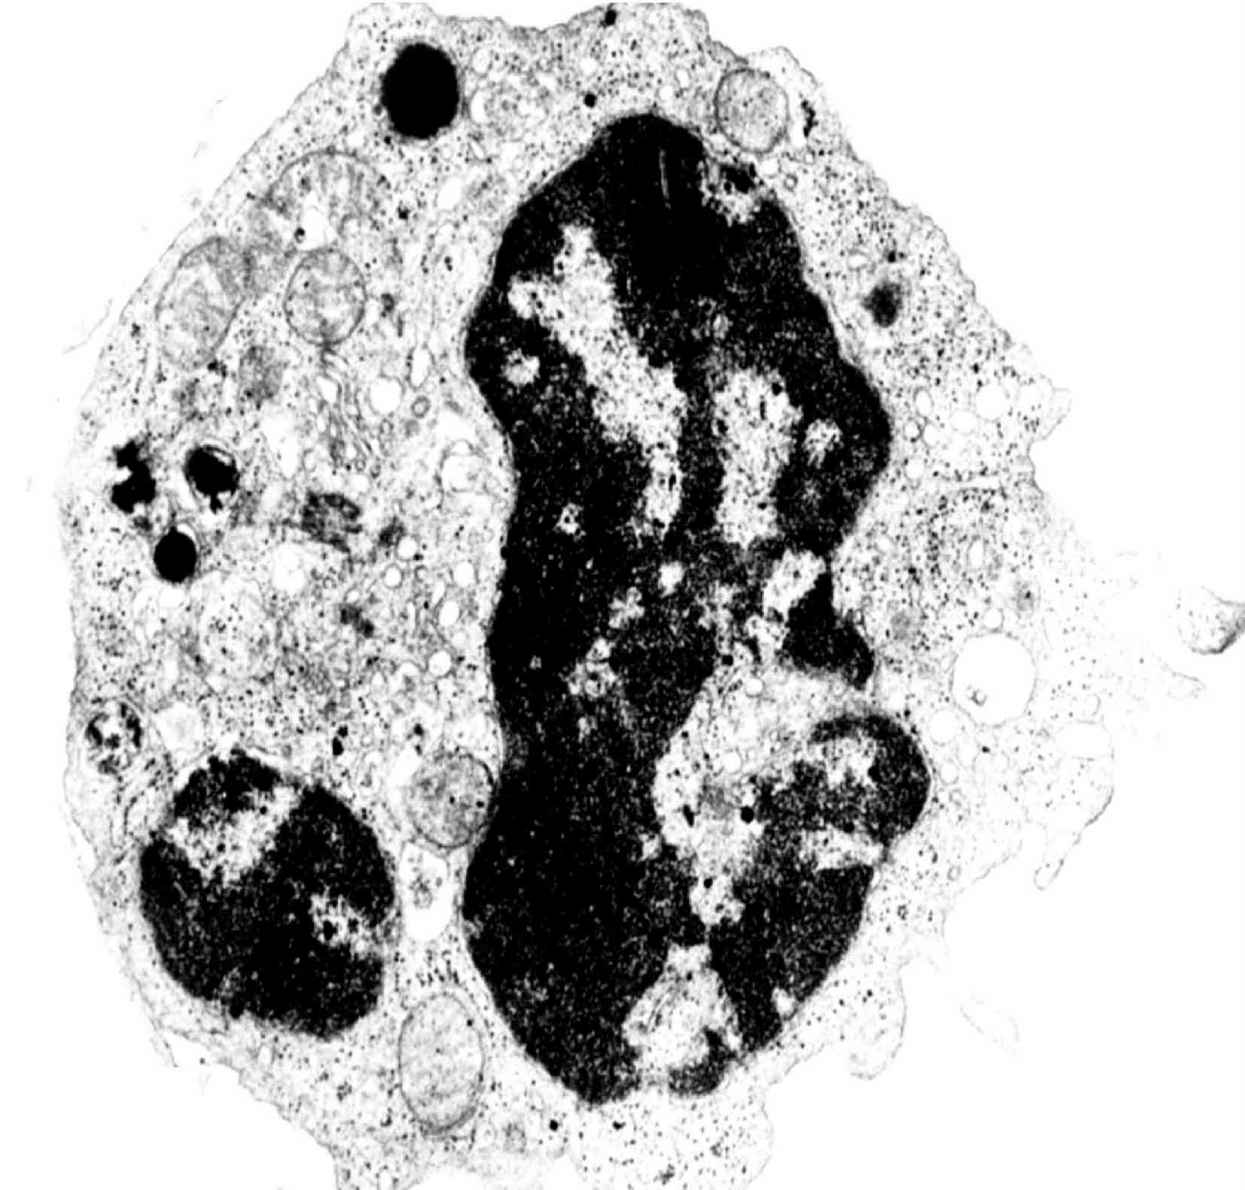
\includegraphics[width=5.90625in,height=2.69792in]{./images/Image00044.jpg}
\end{table}

识别咳嗽的不同特征有助于诊断,包括什么时候开始咳嗽?咳嗽是日间重抑或夜间重?多痰或干咳?痰液的性状如何以及咳嗽伴随什么症状?

健康状态良好的慢性咳嗽,多见慢性咽、喉炎及支气管炎,也可见于支气管扩张。经常作咽部清除动作的咳嗽和咳出黏痰,尤其起床后出现者,多为上气道咳嗽综合征(upper
airway cough
syndrome,UACS)。间歇性咳嗽伴有喘息者多为支气管哮喘。如果每年都在同一时间发作的咳嗽,可能为过敏性鼻炎。日间高声干咳,引起虚脱,伴有情感性反应者提示心因性咳嗽。呈进行性消瘦的慢性咳嗽患者,须注意为消耗性疾病,如肺结核、肺部恶性肿瘤等。

反复咳出大量脓痰者常为肺脓肿,这些患者每有醉酒、昏迷或肺部急性炎症感染病史。如于童年起病,脓痰在经过中逐渐增多,多见于支气管扩张。肺脓肿和支气管扩张的排痰量与体位改变有一定关系。伴有血痰的慢性咳嗽多见于肺结核、肺癌、支气管扩张、慢性肺脓肿、肺吸虫病、淤血性支气管炎等,有时也可见于慢性支气管炎。干咳有服用血管紧张素转换酶抑制剂(ACEI)者要注意药物诱发的咳嗽。

伴有胸痛的慢性咳嗽,常见于肺部病变波及胸膜或附近骨膜,如肺结核、支气管肺癌等。难以忍受的胸部闷痛,须注意支气管肺癌的可能。

长期与有害粉尘接触的慢性咳嗽患者,须注意尘肺的可能性。仰卧时突然发生咳嗽,口腔伴有酸味者提示胃食管反流。

细致的体格检查对60\%病例有诊断价值。体检可发现:咽充血,黏膜可伴有或没有炎性肿胀和脓性分泌物,见于鼻窦炎、上气道咳嗽综合征或过敏性疾病。双肺弥漫性吸气性湿啰音见于肺水肿或肺纤维化。呼气性哮鸣音,见于哮喘或慢性阻塞性肺疾病。散在的湿啰音咳嗽后改变或消失者见于支气管炎。固定的局限性湿啰音见于支气管扩张。肺尖部局限性小湿啰音常提示浸润性肺结核。局限性上肺野大、中湿啰音常提示空洞性肺结核。慢性咳嗽伴杵状指须注意支气管扩张,慢性肺脓肿,慢性肺性骨关节病,特发性肺纤维化。伴颈部及锁骨上淋巴结肿大须注意肺结核、肺癌。

\section{(二)痰检查}

纤维素性支气管炎痰中出现树枝状管型物。痰的细菌学检查(涂片、培养、PCR)对慢性气道和肺部炎症、肺结核、肺真菌病等的诊断有重要意义。痰细胞学检查发现癌细胞能明确肺癌的诊断,痰发现嗜酸性粒细胞增高是诊断嗜酸性粒细胞支气管炎(eosinophilic
bronchitis,EB)的主要指标。

\section{(三)器械检查}

\subsection{1.胸部X线透视及摄片检查}

能进一步确定肺部病变的部位、范围与形态,有时也可确定其性质,如肺部炎症、肺结核、肺脓肿、肺癌、肺囊肿、尘肺等。对于肺深部病变,则X线体层摄片、CT、MRI等诊断价值较大。鼻窦X线检查也有助于寻找咳嗽的病因,可以发现鼻窦炎或鼻窦积脓。胸部CT的横断面图像并无影像重叠,可发现X线胸片未能显示的病灶和小病灶,对肺间质性病变,可较早期清晰显示细小结节及网状阴影。

\subsection{2.纤维支气管镜检查}

对慢性咳嗽患者有时是必需的,可发现大气道内炎症、肿物、异物,并可做活检、支气管肺泡灌洗等。喉镜、鼻咽镜对上呼吸道病变的诊断也是必需的。胸腔镜检查对弥漫性肺疾病和胸膜疾病引起的咳嗽有重要的诊断价值。纵隔镜检查对纵隔病变有时也是必需的。

\subsection{3.支气管激发试验和舒张试验}

可诊断咳嗽变异性哮喘和其他气道过敏性疾病。最大呼气流量(PEF)变异率的测定可评价患者的气道功能状态。

\subsection{4.咳嗽敏感性检查}

通过雾化方式使受试者吸入一定量的刺激物气雾溶胶颗粒,刺激相应的咳嗽感受器而诱发咳嗽,并以咳嗽次数作为咳嗽敏感性的指标。常用辣椒素吸入进行咳嗽激发试验。咳嗽敏感性增高常见于AC、EB、GERC。

\subsection{5.24小时食管内pH监测}

可诊断胃食管反流引起的咳嗽。

\protect\hypertarget{text00063.html}{}{}

\section{13 慢性鼻、咽、喉疾病}

\subsection{一、上气道咳嗽综合征}

上气道咳嗽综合征(UACS)最早源于2006年美国胸科医师协会(ACCP)慢性咳嗽指南,用于代替过去文献中所用的鼻后滴流综合征(postnasal
drip
syndrome,PNDS),后者是指由鼻部疾病引起分泌物倒流至鼻后和咽喉部甚至反流入声门或气管,引起以咳嗽为主要表现的综合征。而UACS的定义为由鼻及鼻窦病变引起的以咳嗽为主要症状的综合征,伴或不伴PNDS,是导致慢性咳嗽的重要原因之一,咳嗽常超过8周,其患病率占慢性咳嗽的22.0\%~57.6\%。本病以慢性咳嗽、咳痰为主要临床表现,常伴有打喷嚏、鼻痒、鼻分泌物增加和鼻塞等,可有鼻后滴流感、面部疼痛及嗅觉障碍。常伴有下列体征:清喉动作、咽部黏膜充血、淋巴滤泡增生(可呈鹅卵石样外观)、咽后壁有黏性分泌物附着等。上述临床症状和体征无特异性,基础疾病的确诊尚需进一步检查。

临床诊断需综合基础疾病、咳嗽与相关症状、鼻咽检查及治疗反应进行综合诊断。我国2009年慢性咳嗽指南提出的诊断标准如下:①发作性或持续性咳嗽,以白天咳嗽为主,入睡后较少咳嗽;②鼻后滴流及(或)咽后壁黏液附着感;③有鼻炎、鼻窦炎、鼻息肉或慢性咽喉炎等病史;④检查发现咽后壁有黏液附着、鹅卵石样观;⑤经针对性治疗后咳嗽缓解。

\subsection{二、慢性咽炎}

\subsubsection{(一)慢性单纯性咽炎}

慢性单纯性咽炎是常见的咽部疾病,其突出的症状为刺激性干咳。由于咽部有瘙痒感及不适感,患者常作廓清咽部的动作,且在讲话多时症状更为显著。患者在讲话中,常须中断,并作吞咽动作以减轻症状。

咽部检查可见咽部充血,咽后壁黏膜表面可见许多扩张的毛细血管及少量淋巴滤泡增殖,咽后壁黏膜及腭弓可略增厚,分泌物可能增多,也可在咽后壁黏膜上发现有黏稠的分泌物附着。

慢性咽炎诊断较易,但病因颇多,须明确其病因,才易于防治。慢性单纯性与慢性增殖性咽炎可由急性咽炎反复发作而来,而大多数继发于上呼吸道病变,如鼻炎、鼻窦炎或口腔慢性炎症。有害粉尘、气体的吸入及烟酒过度等,均可为本病的原因。

\subsubsection{(二)慢性增殖性咽炎}

慢性增殖性咽炎的症状与单纯性咽炎相似,但较显著。

咽部检查可见咽部充血、血管扩张、软腭充血,悬雍垂也可充血、水肿,由于淋巴滤泡增殖、互相融合呈现颗粒状。淋巴滤泡增殖常阻塞咽后壁腺管开口,而致腺体分泌淤积扩大,增加了咽后壁肿胀的程度。咽扁桃体肿大可引起咽鼓管口阻塞而产生耳鸣、听力减退。患者的咽反射特别敏感,常易引起恶心。

\subsubsection{(三)慢性萎缩性咽炎}

咽干燥感是此病最突出症状,患者每于饮水后症状减轻。萎缩的黏膜上被覆痂皮时,常导致干咳、异物感及瘙痒感。

咽部检查发现黏膜苍白、干燥、菲薄而光滑,病变较重者,其上覆盖干燥黏液与痂皮。咽肌萎缩,咽腔似甚宽广。

慢性萎缩性咽炎常继发于萎缩性鼻炎,或咽手术、咽部放射性治疗之后。

\subsection{三、慢性喉炎}

\subsubsection{(一)慢性单纯性与增殖性喉炎}

慢性单纯性与增殖性喉炎的症状以声嘶为主,早期常间歇发生,且每于发音较多时出现。如病情加重,声嘶可成持续,但完全失音者尚属罕见。此外,喉部常有瘙痒、灼热、刺痛等感觉,因此患者常作干咳以减轻症状。

间接喉镜检查时,早期(慢性单纯性喉炎)患者喉部黏膜充血,声带丧失其原有色泽,且可见其上分布有扩张的血管,声带上或杓状间隙可见黏性分泌物黏附。病情加重时(即慢性增殖性喉炎),则黏膜呈暗红色,并有明显增厚,声带暗红,边缘肥厚而呈钝圆,发音时常因声带肥厚而闭合不全,喉室带因代偿活动而致增厚,其较重者可掩盖声带的一部分或全部。

\subsubsection{(二)慢性萎缩性喉炎}

此病比较少见,其主要症状为刺激性干咳,有时甚至可引起声门痉挛。咳嗽之后常咳出黄绿色的痂皮,由于咳嗽用力较猛,每使黏膜损破,以致咳出物带有血丝。声音嘶哑常于痂皮在喉中积聚较多时明显,痂皮排出后好转。由于喉肌萎缩,除声音嘶哑外,常显得软弱无力。此外喉部有灼热感及痛感。

间接喉镜检查时,可见黄绿色或黑绿色痂皮,其严重者甚至在气管内也有痂皮发现。

\subsection{四、咽结核与喉结核}

咽结核与喉结核常继发于开放性肺结核。咽结核的早期,常于水肿、苍白的咽峡、软腭或甚至舌根部出现灰白色结节;此时患者只觉咽部不适,至结节破溃形成溃疡后,才出现咽痛与吞咽痛。疼痛常很明显,患者常因此而拒食。溃疡可发生于咽部各处甚至舌部。溃疡发展缓慢、浅表、边缘不整如鼠咬状,其上附有黏液,但底部较清洁,此外患者常有发热、唾液分泌增多、消瘦及咳嗽等症状。

喉结核早期症状每为干咳及轻度声嘶,声嘶往往出现于下午或晚上,随病情加剧而声嘶越加显著,到后期不仅声嘶而且发音无力,形同耳语。喉部因分泌物积聚而常诱发持久的严重咳嗽。喉部及喉咽部疼痛明显,并常反射至耳部。吞咽痛尤剧烈,进食困难的程度较咽结核更为严重。

喉结核患者咽部黏膜显得苍白,间接喉镜检查,早期常见杓状间隙及会厌披裂后部肿胀,有时早期患者也有出现会厌肿胀的;肿胀之处黏膜均苍白,并有黏液附着于杓状间隙。声带甚至喉室带、会厌等处先后出现溃疡,其严重者喉部形态不能分辨。

\subsection{五、喉 癌}

喉癌常出现咳嗽和声音嘶哑等症状。诊断须经专科医生检查。

\protect\hypertarget{text00064.html}{}{}

\section{14 慢性支气管疾病}

\subsection{一、慢性支气管炎}

患者每年咳嗽、咳痰达3个月以上,连续2年或更长,并可除外其他已知原因的慢性咳嗽,可以诊断为慢性支气管炎。如果肺功能检测FEV\textsubscript{1}
/FVC<70\%,则为慢性阻塞性肺疾病(COPD)。引起慢性支气管炎的内因是机体及呼吸道局部抵抗力降低,外因主要是细菌或病毒感染,有害气体、尘埃的吸入,过冷、过热、过于干燥的空气的刺激以及过敏因素等。

慢性支气管炎多见于中年以上,每于冬春季加剧,夏季减轻或缓解。最突出的症状是咳嗽,尤其是清晨醒后较剧,也可在夜间加剧而致影响睡眠,咳出或多或少的脓性黏液痰,有时也可发生小量咯血。可有微热与全身不适。听诊有散在性干啰音与中、小湿啰音,但也可无明显听诊体征,后期往往并发肺气肿,X线检查可见肺纹理增粗与肺气肿等征象。

慢性支气管炎的诊断,主要应用排除法,即排除其他原因所致的慢性咳嗽而确定之。淤血性支气管炎的患者,有器质性心脏病的体征,每于劳动后或夜间平卧时咳嗽增多。支气管内膜结核,常发生于有开放性肺结核病灶的患者,表现为阵发刺激性咳嗽,有时很难制止,常有哮鸣音,痰中带血,痰抗酸染色可发现抗酸杆菌。支气管镜检查有助于诊断。支气管扩张,每以长期咳嗽、反复大量脓痰或咯血为主要症状,胸部CT、必要时支气管造影可确定诊断。长期接触有害粉尘的慢性咳嗽患者,须注意为尘肺的可能。呼吸道真菌病,其临床表现无特殊,多有长期顽固性咳嗽,咳黏稠痰或带血痰。常发生于身体衰弱或长期使用广谱抗菌素、皮质激素的患者,痰真菌检查发现真菌及菌丝,多次培养阳性及动物接种可助确诊。支气管肺癌发病多在中年以上,可有吼哮样刺激性咳嗽,常持续咯血痰,色鲜红或带褐红色,痰可找到癌细胞,胸部X线检查及支气管镜检查有助于诊断。肺吸虫病及肺包虫病,有地区性流行病学供参考,前者痰常呈铁锈色,痰中易发现肺吸虫卵;肺包虫病多见于牧区,胸部X线检查有特殊征象(参见第30节)。

\subsection{二、淤血性支气管炎}

慢性左心衰竭患者由于支气管黏膜长期淤血,常有持久的咳嗽,多在夜间平卧时或活动后加剧。体检发现两侧肺底弥漫性中、小湿啰音。国内曾见文献报道以慢性咳嗽为首发症状的左心功能不全,使用利尿剂作诊断性治疗,用利尿剂后能降低心脏前负荷,较快地解除了肺淤血和支气管黏膜水肿,从而在排尿后的5~10分钟即表现出镇咳效应。慢性心血管疾病的咳嗽,除由淤血性支气管炎引起之外,尚可能由于主动脉瘤、增大的左心房和扩大的肺动脉压迫气管、支气管,或合并支气管感染、支气管肺炎等所致。在诊断淤血性支气管炎时,上述原因须加以排除。

此外,国内曾报道一例以顽固性咳嗽为表现的室性期前收缩,患者室性期前收缩发作时出现刺激性咳嗽,经给予普罗帕酮治疗后咳嗽消失。

\subsection{三、嗜酸性粒细胞性支气管炎}

嗜酸性粒细胞性支气管炎(EB)是1989年由Gibson等首先定义的一种疾病,为一组痰嗜酸性粒细胞增多,对糖皮质激素敏感,但肺功能正常,无气道高反应性(AHR)的证据,最大呼气流量(PEF)变异率正常的非哮喘慢性咳嗽。主要症状为慢性咳嗽,或晨起咳少许黏痰。部分患者对油烟、灰尘、异味或冷空气比较敏感。目前的研究认为EB是不明原因慢性咳嗽的一个重要病因,大约占慢性咳嗽的10\%~20\%。肺功能和诱导痰检查是诊断EB主要的实验室检查。其诊断标准:①慢性咳嗽,表现为刺激性干咳或伴少量黏痰;②X线胸片正常;③通气功能正常,气道高反应性阴性,呼气峰流速日间变异率正常;④痰细胞学检查嗜酸性粒细胞比例≥2.5\%;⑤排除其他嗜酸性粒细胞增多性疾病;⑥口服或吸入糖皮质激素有效。

EB需和一些肺部寄生虫感染性疾病(如肺吸虫)相鉴别,肺部寄生虫感染也可以表现为慢性咳嗽,少数痰中可见到嗜酸性粒细胞增多,但其外周血中嗜酸性粒细胞明显增高,胸片多有异常,吸入糖皮质激素治疗无效而驱虫治疗有效。

\subsection{四、弥漫性泛细支气管炎}

弥漫性泛细支气管炎(DPB)于1969年由日本学者发现,是一种弥漫存在于两肺呼吸性细支气管区域的气道慢性炎症性疾病。至今病因尚不清楚,可能与人种、遗传因素有关。DPB的受累部位主要是呼吸性细支气管以远的终末气道,病理学特点是炎症病变弥漫性地分布并累及呼吸性细支气管壁的全层。突出的临床表现是咳嗽、咳痰和活动后气促。严重者可导致呼吸功能障碍。在有大环内酯类抗生素疗法之前,DPB多数预后不良,5年生存率只有5\%左右,而大环内酯类抗生素疗法(十四元环、十五元环大环内酯)开展以来已提高到95\%。

本病诊断标准:必备条件:①持续性咳嗽、咳痰、活动时呼吸困难;②合并有慢性鼻窦炎或有既往史;③胸部X线可见两肺弥漫性散在的颗粒样结节状阴影或胸部CT可见两肺弥漫性小叶中心性颗粒样结节状阴影。参考条件:①胸部听诊断续性湿啰音;②一秒钟用力呼气容积(FEV\textsubscript{1}
)占预计值百分比降低(<70\%)以及低氧血症(PaO\textsubscript{2}
<80mmHg);③血清冷凝集试验(CHA)效价增高(>1∶64)。确诊:符合必备条件①、②和③加上参考条件中的2项以上;一般诊断:符合必备条件①、②和③;可疑诊断:符合必备条件①和②。

本病近年国内已有报道。需要和本病相鉴别的是一些临床表现、影像学或病理改变相类似的疾病,如COPD、支气管扩张、支气管哮喘、粟粒型肺结核、结节病、癌性淋巴管炎、肺泡细胞癌、纤毛不动综合征、呼吸性细支气管炎伴间质性肺病(RBILD)和慢性外源性过敏性肺泡炎等,X线胸片、高分辨率CT(HRCT)、病理组织学检查等是主要的鉴别手段。也可通过大环内酯类抗生素进行治疗观察。

\subsection{五、咳嗽变异型哮喘}

咳嗽变异型哮喘(CVA)是以咳嗽为其唯一症状的哮喘,患者无发作性的喘息、气急,双肺无哮鸣音。目前发现约6.5\%~57\%的慢性咳嗽的真正原因为CVA。患者常常具有过敏性疾病或哮喘家族史,或同时患有过敏性鼻炎。咳嗽多为刺激性干咳,发作频繁、剧烈,下半夜咳嗽是其特征。可由于上呼吸道感染、运动、冷空气吸入以及过敏原等刺激而诱发并加重。支气管激发试验常阳性,提示气道高反应性,按照支气管炎给予止咳和抗生素治疗无效,而按哮喘给予支气管舒张剂和吸入糖皮质激素治疗可奏效。CVA患者若不能得到及时诊断及治疗,多数可逐渐发展为典型哮喘。

CVA的诊断要点为:①慢性持续性干咳达1~2个月以上,伴有夜间咳嗽或运动性咳嗽,经正规抗生素及止咳祛痰药物治疗无效;②气道呈高反应性;③泼尼松试验阳性或支气管舒张剂能显著改善咳嗽症状;④除外其他导致慢性干咳的病因。

\subsection{六、变应性咳嗽(atopic cough)}

变应性咳嗽是1992年由日本的学者Fujimura首先定义的一种疾病诊断,表现为变应性非哮喘性慢性干咳,支气管扩张剂无效,肺功能正常,无气道高反应性的证据,峰流速变异率正常,抗组胺药或糖皮质激素治疗效果良好。本病与变应性咽喉炎、EB、感冒后咳嗽的关系及异同还有待进一步明确。其主要临床表现为刺激性干咳,多为阵发性,白天或夜间咳嗽,油烟、灰尘、冷空气、讲话等容易诱发咳嗽,常伴有咽喉发痒。

本病目前尚无公认的标准,中华医学会提出的诊断标准可供参考:

(1)慢性咳嗽。

(2)肺通气功能正常,气道高反应性检测阴性。

(3)具有下列指征之一:①过敏物质接触史,②变应原皮肤针刺试验阳性,③血清总IgE或特异性IgE增高,④咳嗽敏感性增高。

(4)排除CVA、EB、UACS等其他原因引起的慢性咳嗽。

(5)抗组胺药物及(或)糖皮质激素治疗有效。

我国的标准与日本相比,不包括诱导痰和外周血中嗜酸性粒细胞增高,其他基本相同。该病与哮喘、CVA、EB鉴别见表\ref{tab5-2}。

\subsection{七、百日咳}

百日咳是常见的小儿急性传染病,病原体为百日咳杆菌,在儿童集体中易发生流行。病初期表现为急性上呼吸道感染症状(卡他期),约1~2周后出现阵发性痉挛性咳嗽(痉咳期),伴以深长的鸡鸣样吸气声,咳嗽约经2~6周而逐渐缓解(恢复期)。有时也迁延较久,甚至达一年以上。得病后可遗留痕迹反射,一年之内再罹患呼吸道疾病而发生咳嗽时,可出现百日咳样咳嗽。

如病儿咳嗽、咳痰久未康复,须考虑陈旧性肺结核病灶再度活动或继发支气管扩张。

\begin{table}[htbp]
\centering
\caption{EB、哮喘、CVA、AC的临床特征}
\label{tab5-2}
\includegraphics[width=5.9375in,height=2.83333in]{./images/Image00045.jpg}

注:*当痰中EOS增多时
\end{table}



\subsection{八、支气管扩张}

慢性咳嗽是本病的特征之一,干性型支气管扩张患者咳嗽较少,典型者则常咳出大量浆液脓性痰液,并常于晨间或变换体位时咳嗽加剧,患者可有咯血以及同一部位反复发生肺炎(参见第12节)。

\subsection{九、气管、支气管结核}

气管、支气管结核又称支气管内膜结核(EBTB),是指发生在气管、支气管黏膜和黏膜下层的结核病。活动性肺结核中大约10\%~40\%伴有EBTB。主支气管、两肺上叶、中叶、舌叶支气管为好发部位。EBTB起病缓慢,症状多样,缺乏特异性。症状多为咳嗽(刺激性咳嗽为主者较多)、咳痰、低热、盗汗、呼吸困难、体重减轻、咯血(少数病例)、胸痛等;体检少数患者可有肺部局限性哮鸣音、局限性呼吸减弱等;胸片示肺纹理密集、肺纹理粗乱、肺不张、局限性肺气肿等,与慢性支气管炎、肺癌、肺真菌病,甚至支气管哮喘相似,易误诊。有作者报道28例单纯型EBTB(指肺内无结核病灶者)的误诊主要由于:①胸片无结核病灶发现;②胸片虽有肺纹理密集粗乱、局限性肺气肿、叶间胸膜移位等异常,但又非特异性,故未及注意而误诊。

近年的研究提示有下列情况应考虑EBTB的可能:

(1)出现原因不明刺激性咳嗽,反复痰血、呼吸困难、喘鸣和胸部不适。

(2)有下列影像学改变者:①出现变化较快的肺不张、局限性肺气肿;②一侧或两侧肺反复出现支气管播散病灶;③时大时小的张力性空洞或空洞内有气液平面;④肺内无明显病灶,但痰抗酸染色阳性;⑤多部位支气管损害,管腔狭窄、扭曲、变形。周围无明显软组织块影。

(3)纤支镜检查对确诊EBTB有决定性作用。建议对凡有干咳、胸闷、喘鸣、咳黏液痰者,经抗炎、对症治疗2周未见好转时及早作纤支镜检查,镜下刷检涂片染色找抗酸杆菌,及(或)做活检送病理组织检查。如无发现而患者疑似本病时,2周后再做纤支镜刷检抗酸杆菌与活检标本病理检查。目前PCR已用于结核病的病原学诊断,对诊断有进一步帮助。

气管、支气管结核的诊断标准如下:①结核病临床表现及临床治疗反应;②痰涂片、集菌抗酸杆菌阳性,最好是培养MTB阳性;③影像学改变;④PPD试验阳性;⑤支气管镜下直视的气管、支气管典型病变;⑥支气管刷片或支气管冲洗液抗酸杆菌阳性;⑦经支气管镜活检组织提示结核性病理改变。符合具备上述5+6、5+7、5+2为确诊标准,1+2+3、1+3+4、2+3、3+4、5、6、7为高度疑诊标准。

\subsection{十、真菌性支气管炎}

真菌性支气管炎比较少见,常继发于全身衰弱、营养不良的患者,长期接受糖皮质激素与广谱抗生素治疗的患者,接受放射治疗、化学治疗的恶性肿瘤患者,或慢性肺部疾病的患者。但也可原发性发病(参见第17节)。

\subsection{十一、纤维素性支气管炎}

纤维素性支气管炎又名纤维蛋白性支气管炎、管型支气管炎和成型支气管炎等,临床上较少见。病因、病理和发病机制尚未完全清楚,多继发于支气管炎、肺结核、心力衰竭等。目前多认为发病机制与变态反应有关,可能是特异质患者在各种致病因子作用下,呼吸道黏膜发生变态反应,使血管壁通透性增强,炎性物质和纤维蛋白渗出,腺体分泌亢进,细胞浸润聚集于管腔内。在组织凝血酶和黏液酶及管腔内pH值改变的作用下,分泌物脱水、浓缩、凝固,从而铸成支气管样管型。又因机体的排异作用,使管型剥离而损伤小血管,导致咯血。

本病常见的临床表现为咳嗽,可为剧咳或呛咳,管型咯出前有胸闷、气憋或窒息感;咯血,多少不等,一般50~1000ml,咯血前咽部奇痒或咽部有阻塞感;咯出支气管管型,为树枝状膜样管型物,灰白色、淡褐色或浅红色,咯出管型后咳嗽、胸闷、窒息感可迅速缓解。咯出的管型清水漂洗后常可见典型的支气管管型,大体上呈树枝状、膜片状,柔韧性好,不易碎裂。管型一般长约5~6cm,最长可达30cm,主干中空,末端变细,有的呈丝状。镜下检查为红染均质的纤维素,中间混有多少不等的中性粒细胞、嗜酸性粒细胞及淋巴细胞。体检肺部呼吸音减低或可闻及干湿啰音,血象白细胞可轻度增高,合并细菌感染者可显著增高并伴发热。胸部X线检查一般正常,极少数可在肺门区或心缘旁有尖端向内的楔形或Y形阴影或表现为局限性肺不张,但均无特异性诊断价值。纤支镜检查可发现附着于气管或支气管的管型,有助于诊断。

\protect\hypertarget{text00065.html}{}{}

\section{15 慢性肺部疾病}

\subsection{一、原发性支气管肺癌(肺癌)}

原发性支气管肺癌简称肺癌,指肿瘤细胞源于支气管黏膜或腺体。肺癌按解剖学部位可分为中央型肺癌和周围型肺癌,前者发生在段支气管至主支气管,约占3/4,以鳞状上皮细胞癌和小细胞未分化癌较多见;后者发生在段支气管以下,约占1/4,以腺癌较为多见。肺癌按组织病理可分为非小细胞肺癌(NSCLC)和小细胞肺癌(SCLC),前者包括鳞状上皮细胞癌(鳞癌)、腺癌、大细胞癌、腺鳞癌、类癌、支气管腺体癌等;后者包括燕麦细胞型,中间细胞型、复合燕麦细胞型。

早期肺癌大多无症状或体征,当出现以下临床表现时应警惕肺癌的可能,尤其是对于40岁以上有长期吸烟史(吸烟指数>20包年)者,应尽快行胸部影像学检查明确:

1.持续性无痰或少痰的刺激性咳嗽,或原有慢性咳嗽的性质发生改变。

2.咯血或痰中带血。

3.气短或喘鸣,听诊时可发现局限或固定性哮鸣音。

4.发热,抗生素治疗效果不佳。

5.体重下降。

6.同一部位反复发生肺炎。

7.出现原因不明,久治不愈的肺外征象,如杵状指(趾)、非游走性肺性关节疼痛、男性乳腺发育、皮肤黝黑或皮肌炎、共济失调。

8.出现局部侵犯及转移的体征,如声带麻痹、上腔静脉压迫综合征、Horner综合征、Pancoast综合征、锁骨上窝淋巴结肿大等。

肺癌的诊断,主要采取综合诊断方法。

胸部X线检查普及率广、应用方便、辐射量小,但分辨率低,不易检出肺内隐蔽部位病灶和微小病灶,在早期肺癌的检出应用方面有一定局限性。早期肺癌的X线征象主要有以下几种:

1.局限性肺气肿
支气管内极小的癌瘤,X线检查常无异常发现,当肿瘤长大引起支气管部分性阻塞,空气入易出难,则在阻塞远端的肺组织形成局限性肺气肿。局限性肺气肿是肺癌早期征象之一。在透视或摄片时作呼气检查,较易观察到肺气肿部分与其他部分肺脏的对比。

2.肺不张
肿瘤完全阻塞支气管时则引起肺不张。临床上发现年龄较大的肺不张患者,应考虑肺癌的可能性。

3.一侧肺门阴影增宽
此种阴影是由癌、淋巴结肿大及癌周围组织炎症病变所构成,边缘多呈毛刺状,是中央型肺癌最常见的X线征象。如有淋巴结转移,可认为是较晚期的表现。

4.孤立性结节阴影
早期的周围型肺癌常呈小的圆形或椭圆形结节阴影,边缘常不整齐,常凹入或分叶状;结节阴影绝大多数为单发性。如为大小相似的多发性阴影,大概不是原发性肺癌(参见第31节)。

5.不消散的或反复出现的节段性肺炎。

当肺癌在支气管内继续生长和分泌物引流受阻时,则可引起阻塞肺段的局限性肺炎。此种肺炎虽经积极的抗生素治疗仍不消散。

肺癌的早期诊断还须依靠下列检查:

\subsubsection{1.痰细胞检查}

痰液脱落细胞检查是目前诊断肺癌简单方便的无创伤性诊断方法之一,连续三天留取清晨深咳后的痰液进行痰细胞学涂片检查可以获得细胞学的诊断。液基细胞学可以提高诊断率。高质量的痰标本和标本优化处理是提高细胞学检查阳性率的重要保证。有报告阳性率可达80\%,其优点是不致增加患者的痛苦,易于接受。可嘱患者清晨漱口后,用力咳出第二、三口痰立即送检。阴性时反复多次送检。

\subsubsection{2.纤维支气管镜检查}

可直视下刷检或(及)钳夹活检,或透视指导下经纤支镜肺活检,或经支气管针刺吸引活检。目前应用荧光支气管镜和超声支气管内镜技术(EBUS)对支气管内病变组织及支气管周围肿大淋巴结的活检提高了肺癌的诊断率。

\subsubsection{3.CT和PET/CT}

是一种无创伤性检查方法,患者易于接受,可检出早期肺癌,是目前诊断肺癌的重要手段。可以提示病变所在的部位和累及范围,可为区分其良恶性提供重要参考意见。对肺内病灶,特别是纵隔和心影后的病灶,CT检查可比X线检查显示较清楚的影像。低剂量CT(LDCT)可以有效地发现早期肺癌,已经逐步取代胸片成为较敏感的肺结节评估工具。美国胸外科学会推荐对年龄在55~79岁、吸烟指数达30包年的成人每年进行低剂量螺旋CT进行肺癌筛查,而对于吸烟指数达20包年且预计5年累积肺癌发生率在5\%以上的成人,筛查起始时间应提前至50岁。

\textsuperscript{18}
F-脱氧葡萄糖(F-18fluoro-deoxyglucose,FDG)正电子发射断层显像(positron
emission
tomography,PET)正电子断层扫描仪将人体代谢所必需的物质如葡萄糖、蛋白质、核酸、脂肪酸等标记上具有正电子放射性的短寿命核素,制成显像剂(如氟代脱氧葡萄糖)注入人体后进行扫描成像。放射性\textsuperscript{18}
FDG注入体内后,肿瘤组织对其摄取率明显增加,从而被探测系统记录,经计算机图像重建显示三维断层图像。因此,PET有助于胸片或CT检查发现病变的定性诊断,以及肺癌治疗前后的疗效判断。有学者报道PET用于CT不能定性的病变诊断肺癌的敏感性高达95\%。PET可以弥补螺旋CT定性困难的不足。该检查有助于无创性鉴别良恶性结节,甚至还可为选择病灶进行活检或穿刺检查提供重要参考意见,在高代谢的病灶处活检更容易获得可靠的结果。但鉴于其价格昂贵,不推荐作为常规检查。对5mm以下的病灶或磨玻璃样阴影其诊断价值受到限制。

\subsubsection{4.磁共振显像(MRI)}

是一种非侵入性检查,已用于肺癌的诊断。它与CT二者各有优点,可互相补充。CT能全面地显示病灶范围,但对中心型小结节,有时易误认为肺血管断面,而MRI观察血管有良好的天然对比(流空效应),故可鉴别肺门或纵隔内的肿物是否为血管性或非血管性。MRI较增强CT更好地显示肺门及纵隔内的淋巴结和肿块,但CT在检测气管及支气管病变方面则优于MRI。

\subsubsection{5.其他器械检查}

近年来,更多的检查用于肺癌的诊断,包括单光子发射计算机断层扫描(SPECT)、经胸壁细针穿刺活检、纵隔镜检查、胸腔镜检查、开胸肺活检等,可根据需要选用。

\subsubsection{6.血清肿瘤标志物检查}

目前尚无特异性肺癌标志物应用于临床诊断,但部分标志物可作为肺癌诊断或者评估肺癌治疗效果的参考。如在随访阶段发现肿瘤标志物水平进行性升高,需积极进行下一步检查。现阶段,常用的血清肿瘤标志物有以下几种:

\paragraph{(1)癌胚抗原(carcinoembryonic antigen,CEA):}

主要用于肺癌诊断和判断预后以及对治疗过程的监测。

\paragraph{(2)细胞角蛋白片段19(cytokeratin fragment,CYFRA21-1):}

对肺鳞癌诊断的敏感性、特异性有一定参考意义。

\paragraph{(3)鳞癌抗原(squamous cell carcinoma antigen,SCC):}

对肺鳞癌疗效监测和预后判断有一定价值。

\paragraph{(4)神经元特异性烯醇化酶(neuron specific enolase,NSE):}

用于小细胞肺癌的诊断和治疗反应监测。

\paragraph{(5)胃泌素释放肽前体(pro gastrin releasing peptide,Pro-GRP):}

可作为小细胞肺癌的诊断和鉴别诊断的首选标志物。

如患者临床未能排除肺癌,而上述检查阴性,仍须定期作X线胸片与痰中癌细胞检查。对病因未明的反复的或持久性节段性肺炎与肺不张,或周围性结节状病灶无法排除肺癌时,可考虑开胸探查。抗结核的诊断性治疗,一般不应超过4周,以免错过手术根治的机会。

多数作者认为,有症状的肺癌往往已属晚期,无症状者(隐性肺癌)常属早期,故应重视亚临床、无症状病例的发现。对高发区人群和长期吸烟者尤须作定期的普查,以期无症状早期肺癌的发现。

肺癌误诊病例不少,特别是早期肺癌,主要由于:①因年龄在30~40岁以下而不引起注意,致误诊为肺结核、支气管扩张、节段性肺炎等;②由于胸腔积液为浅黄色浆液性,或为包裹性积液而误诊为结核病;③由于有多关节炎症状而误诊为类风湿关节炎或风湿性关节炎;④由于血性心包积液而误诊为原发性心包炎等。偶尔早期肺癌在X线胸片上被肋骨掩盖而致漏诊。

如肺癌引起淋巴结转移、血性胸腔积液、Horner综合征或其他器官(肝、骨、脑、肾等)的转移,则已属晚期现象。

\subsubsection{(一)细支气管-肺泡细胞癌}

细支气管-肺泡细胞癌女性较多见,半数以上有咯血,有较为特别的临床与病理学表现。癌多于肺的边缘生长,不侵犯大支气管。症状发展缓慢渐进,以咳嗽、咳痰、气短较常见。痰量可能甚多,有时可达数百毫升,是与一般早期肺癌不同之点。此型肺癌可有不同程度的炎症、坏死,但极少形成空洞。体征因癌瘤的大小与位置而定,一般较易引起胸腔积液。X线检查可分孤立结节型、弥漫型、肺炎型三种表现,以孤立结节型最多见。由于不同的X线表现,易与肺结核、肺炎、支气管扩张、慢性支气管炎、胸膜炎等相混淆。

细支气管-肺泡细胞癌可有下列临床表现供诊断参考:①病情发展缓慢,自起病至确诊可能经过半年以上;②肿瘤位于肺的外周部分,早期即累及终末支气管与胸膜;③患者每有呼吸困难等缺氧现象;④由于癌细胞可分泌黏液,因而有顽固性咳嗽和咳出大量黏稠、胶冻样的痰液,是部分患者突出的症状。

此型肺癌在支气管造影片上有下列征象:①受累的支气管呈均等而明显的狭窄;②支气管影像呈僵硬、伸长;③造影剂充盈于支气管内而不黏附在壁上;④因支气管的细小分支和肺泡不充盈,所以支气管树呈枯枝状。痰内癌细胞检出率高,有重要诊断意义。又因此型癌细胞易于剥落,支气管肺泡灌洗液沉渣中较易检出癌细胞。

弥漫型细支气管-肺泡细胞癌与急性粟粒型肺结核的X线表现相似,临床上常导致误诊,两者的鉴别可参考表\ref{tab5-3}。

\begin{table}[htbp]
\centering
\caption{弥漫型细支气管-肺泡细胞癌与急性粟粒型肺结核的鉴别}
\label{tab5-3}
\includegraphics[width=5.91667in,height=3.58333in]{./images/Image00046.jpg}
\end{table}

\subsubsection{(二)肺瘢痕癌}

肺瘢痕癌少见。患者多以胸痛、咳嗽、气短、痰中带血为主诉。先期存在的肺瘢痕组织成因多种多样,如尘肺、结核、慢性炎症、支气管扩张、囊肿、异物、梗塞等,尤其以肺结核瘢痕灶的基础上发生的瘢痕癌病例多见。国内报告术后无长期生存的病例。对于肺部有呼吸系统疾病史同时伴有瘢痕形成者,应定期予胸部CT复查、随访。当发现病灶大或密度增高、不均匀,边缘由光整变为不规则甚至出现毛刺、分叶者,应考虑瘢痕癌,必须进一步检查以明确诊断。

\subsubsection{(三)支气管类癌}

少见,主要表现为咳嗽、咯血、发热和反复发作的肺炎。具有发病年龄轻、生长慢、恶性度低、较少转移的特点。应注意与肺癌、结核球及良性肿瘤鉴别。参见第12节。

\subsection{二、肺结核(参见第12.2节)}

\subsection{三、慢性肺脓肿}

急性肺脓肿3个月后未愈,称为慢性肺脓肿,如脓肿周围发生纤维组织增生,常继发支气管扩张。痰量常较多,常有腐臭气味,静置后可分为三层:上层为泡沫;中层为水样浆液层,常为淡绿色;下层为脓层,含有坏死的细胞和碎屑。临床症状往往好转与恶化交替,在间歇期中患者自觉较良好,在恶化期间则症状加重,体温升高,咳嗽,痰量增多,胸痛加剧,血象白细胞增多,并可出现杵状指及肺性骨关节病,内脏(肾、肝)淀粉样变性,贫血和低血浆蛋白性水肿等。

慢性肺脓肿常伴有脓腔周围继发性支气管扩张,须与原发性支气管扩张区别。晚期的支气管扩张也可形成多发性小脓肿,症状与肺脓肿相似。支气管扩张患者常有多年咳嗽、反复咯血和多痰的病史,体检时病变部位可听到多数固定性湿啰音,X线检查可发现支气管卷发样阴影或多发性管状小空腔,胸部CT检查显示管壁增厚的柱状扩张或成串成簇的囊状改变。慢性肺脓肿又须与癌性空洞区别,如经积极抗菌药物治疗,局部支气管阻塞仍未缓解,X线征无好转,空洞壁厚而内缘不规则,呈偏心性,须疑为肺癌,如伴有肋骨骨质破坏则肺癌的诊断大致可以确定。慢性纤维空洞性肺结核也易被误诊为慢性肺脓肿;结核性空洞多位于上肺,空洞内多无气液平面,周围常有结核播散形成的卫星样病灶,一般易于区别。也有少数肺脓肿患者发病不急,痰少,就诊时血象白细胞正常,或呈孤立性空洞,或短期内对青霉素无效,难与结核性空洞鉴别。但肺脓肿病史较短,感染症状比较明显,脓痰多或有臭味。改用有效的抗菌药物可显著好转,慢性病例常发生杵状指或肥大性骨关节病等,痰菌检查有助于二者的鉴别。右下肺脓肿须注意阿米巴肺脓肿的可能,如表现较重的中毒症状,咳棕褐色痰,应怀疑肺阿米巴病,在痰液或脓液中找到溶组织阿米巴或经抗阿米巴治疗奏效可确定诊断。

\subsection{四、肺奴卡菌病}

奴卡菌为放线菌科中的一个属。自从糖皮质激素与免疫抑制剂广泛应用以来,肺奴卡菌病有增加的趋势,国内也有少数病例发现。73\%的奴卡菌病初发于肺脏,可无症状,但多有咳嗽,咳痰、咯血痰、胸痛、脓胸(占20\%)等症状,常伴有发热、乏力、食欲减退、消瘦等全身症状。X线表现无特异性,可有肺炎样、多发性结节、肺脓肿、空洞形成、胸腔积液、粟粒样病灶等征象。易发生血行播散性感染。诊断须根据患者致病诱因、上述临床及X线表现,以及痰、胸腔积液或血培养中证明有奴卡菌存在,以及除外其他原因的肺部病变而确定。

\subsection{五、肺放线菌病}

肺放线菌病国内报告例数不多,发病通常徐缓,开始表现为支气管炎症状,患者有咳嗽,咳黏液痰。当感染侵入肺部引起肺炎或脓肿时,症状加重,咳脓痰或血痰、伴有寒战、发热。可累及胸膜及胸壁。此病的临床症状、体征和胸部X线征象并无特异性,因而早期诊断不易,常被误诊为肺结核、结核性胸腔积液、肺脓肿或肺癌等。如对上述疾病在诊断上有所怀疑,对本病有所警惕,而进行真菌检查,可在痰中或胸腔积液中找到“硫磺颗粒”及培养出放线菌。

此病后期损害肋骨,产生胸壁脓肿及胸壁瘘管形成,此时诊断则较易。在瘘管分泌物中也可找到“硫磺颗粒”及放线菌。

\subsection{六、肺真菌病}

目前在我国常见的肺真菌感染,其致病菌最多为白念珠菌与曲霉,其次为新型隐球菌。此外国内文献还有少数的肺毛霉病报道。前两种多以寄生形式存于人体内,在一定条件下继发呼吸道感染,而新型隐球菌则以原发性致病多见。呼吸道真菌病的临床表现多无规律性,肺部X线表现也形态不一,易侵犯胸膜,可通过血道、淋巴道侵犯神经系统或引起全身播散,常被误诊或漏诊。

临床上有下列一些表现时须考虑肺部真菌病的可能性:

1.老年、幼儿或体弱、营养不良的患者,长期接受广谱抗生素、糖皮质激素、放射线照射或抗肿瘤化学治疗的患者,器官移植患者,病程中出现肺部感染病征。

2.慢性呼吸道疾病如慢性支气管炎、慢性阻塞性肺疾病、支气管扩张、肺结核、慢性肺脓肿等经积极的抗菌药物治疗无效,或病情反而加重者。

3.肺部X线摄片呈粟粒状、斑片状、大片状或圆形块状阴影,而这些病变无特征性改变,即不似肺结核、炎症、肿瘤、寄生虫病等,经抗炎症、抗结核治疗无效或病变反而加重者。

4.经常与家禽、牲畜、稻草、土壤接触或从事酿酒工作,而出现病因未明的肺部病变者。

5.胸壁脓肿、肋骨损害及胸壁瘘管形成。

\subsubsection{(一)肺白念珠菌病}

白念珠菌常侵犯支气管和肺。此种真菌常寄生于正常人的上呼吸道、消化道和皮肤上,感染常为内源性,并在上述1、2两项的致病条件下,使真菌有机会在支气管内繁殖,并进一步侵入肺内。其病程可为急性、亚急性和慢性。

症状比较复杂,一般是慢性进行性,有顽固性咳嗽,咳痰。痰的特点是量少,胶样黏稠或带有乳块状或血丝,如夹杂细菌感染则为脓样。常有发热(38~39℃)、疲乏、盗汗、脉快、纳差、呼吸困难、胸痛等症状。体检所见与其他慢性肺部感染难以区别,可出现啰音、肺实变征、肺空洞与胸腔积液征。此病可与支气管扩张、肺结核、肺脓肿、肺癌等并存。

肺白念珠菌病有下列X线征象:①斑片状阴影;②大片状阴影;③粟粒状阴影;④胸腔积液;⑤肺门淋巴结肿大,肺纹理增多;⑥空洞形成,钙化现象等。

肺白念珠菌病的诊断主要根据:①在无污染的痰液(通常嘱患者早上刷牙后用1\%双氧水含漱10分钟,继用清水漱口,用力咳嗽,弃去第一口痰液、留第二、三口痰液立即送检),或纤支镜检采得的分泌物(此法取材可靠),或胸腔抽出液,多次培养分离出纯种的白念珠菌落,或胸膜活组织病理检查证明有此菌;②临床与X线检查符合此病的表现;③除外肺结核、肺肿瘤、肺脓肿及其他真菌感染(但也可与之并存);④停用抗生素与糖皮质激素,改用抗真菌治疗,有较好的疗效。

\subsubsection{(二)肺曲霉病}

曲霉在自然界分布甚广,一般认为与发霉的谷草、家禽(如鸡、鸭、鸽)、牲畜(牛、羊、马)等接触及酿酒等工作可得此病。肺曲霉感染可以继发于上述1、2两项的致病条件下。

肺曲霉病主要由烟曲霉引起,临床上主要有五种类型:侵袭性肺曲霉病、气管支气管曲霉病、慢性坏死性肺曲霉病、曲霉肿和变应性支气管肺曲霉病(ABPA)。参见第3.1.7节。

起病可急可缓,临床表现多为慢性咳嗽,反复咯血,症状和X线表现可多种多样。侵袭性曲霉病X线特征性改变是以胸膜为基底的多发的楔形阴影或空洞,胸部CT早期的典型表现为晕轮征(halo
sign),后期为新月体征。曲霉肿表现为空洞内有可移动的团球影(曲菌球)。ABPA为上叶短暂性实变或肺不张,中央支气管囊状扩张及壁增厚征象如“戒指征”或“轨道征”。

肺曲霉病临床表现大致可区分为:①类似肺结核、肿瘤或肺脓肿的表现,X线胸片可呈现圆形阴影,有时与肺结核球、肺结核空洞、肺包虫病、肺脓肿不易区别;②反复咯血或咳出大量的泡沫痰(可带有酒味),类似支气管扩张;③急性经过类似大叶性肺炎或小叶性肺炎;④气喘发作类似喘息性支气管炎;⑤全身性多发性小脓肿,呈败血症的病象。

肺曲霉病的诊断主要根据:①有与曲霉接触的职业史。②有上述临床症状和X线改变。③真菌学检查:咳出的深部痰连续三次直接镜检见曲霉丝及芽孢,且培养得到同一型的曲霉支持肺曲霉病的诊断。病理活检发现菌丝及组织培养得到曲霉是确诊的“金标准”。④除外肺结核、肺脓肿、肺癌、支气管扩张及肺炎等疾病,但须注意肺曲霉感染也常继发于上述疾病的基础上而与之并存。⑤抗真菌药治疗有一定的疗效。

\subsubsection{(三)肺隐球菌病}

肺隐球菌病是由新型隐球菌感染引起的一种亚急性或慢性肺部真菌病。主要见于成人,约50\%患者为免疫功能正常的宿主。隐球菌病以中枢神经系统感染最为常见,其次为肺部。一般认为此病首先累及肺部,如果宿主自身免疫力低下,隐球菌不能局限在肺部,就有可能发生全身播散。临床上单独肺部受累的隐球菌病并不多见,仅占全部隐球菌病的13\%~20\%。

本病多无症状,少数患者有干咳、咳少量黏液痰或血丝痰,咯血比较少见,常伴有胸痛、微热、乏力等症状。如有广泛性感染,则出现肺实变体征。本病的影像学表现多样,可呈:①孤立性块影:直径约2~7cm,多见于原发性肺隐球菌病(占81\%);②大片致密影伴小透亮区;③单发或多发性结节影;④单发或多发性斑片状浸润影:常为继发性肺隐球菌病;⑤弥漫性粟粒影;⑥间质性肺炎型:此型少见。⑤⑥常见于免疫功能低下者。另外也可表现为空洞、胸腔积液及肺门淋巴结肿大。影像学的表现无特异性,易与肺癌、肺转移性肿瘤、肺结核、Wegener肉芽肿等疾病相混淆,尤其是孤立性块影与肺癌不易鉴别。

肺隐球菌病的确诊可依靠痰、胸腔积液、支气管肺泡灌洗液、纤支镜病灶刷片、经皮肺穿刺涂片、脑脊液直接涂片加墨汁于光镜下检查;经纤支镜肺组织活检、经皮肺穿刺活检是有价值的确诊手段;间接免疫荧光法在血液中可找到隐球菌循环抗体;必要时行胸腔镜或开胸活检。

\subsubsection{(四)肺毛霉病}

对有免疫功能缺陷的患者,出现呼吸道症状时,须考虑肺毛霉病的可能。临床与X线胸片均无特征性表现。X线表现不一,可为结节状影、多发性小斑片状阴影、肺炎样改变、空洞形成、胸腔积液等。反复做痰、胸腔积液等检查,必要时做肺活检,发现大量毛霉,并除外其他原因的肺部疾病,即可确定诊断。

\subsubsection{(五)肺孢子菌肺炎}

卡氏肺囊虫以前归类为原虫,目前认为是真菌,并命名为孢子菌,侵犯人体的主要为耶氏孢子菌。主要侵犯早产儿和先天性或获得性免疫功能缺陷的人,导致条件致病性感染。健康人偶可罹患。病变绝大多数局限于肺部,主要临床表现为干咳、进行性呼吸困难、发绀,部分患者有发热。呼吸系统症状虽重,但肺部体征甚少或全无,即症状和体征分离,少数患者有肺底湿啰音。淋巴结、肝、脾可肿大。对免疫功能缺陷患者出现上述症状时,应考虑本病之可能。痰及支气管灌洗液中病原体阳性率不高。开胸活检阳性率最高,可达95\%,但并发症多,危险性大。血清特殊性免疫学检查有重要诊断价值。痰和血PCR检测对诊断亦有良好价值。参见第3.1.7节。

\subsection{七、肺寄生虫感染}

\subsubsection{(一)肺(胸膜)阿米巴病}

参见第3.1.8节。

\subsubsection{(二)人类比翼线虫病}

本病亦称喉比翼线虫感染,大多数患者表现为慢性咳嗽。如成虫侵蚀支气管壁,则可引起咳血痰或咯血。咯血多为少量。体重减轻常见。也有咳出鲜红色的Y形线虫而确诊。X线胸片无特异性,可表现为支气管炎或肺炎。广州曾报道三例,一起进食龟后发病,均未到过国外,可认为国内感染,纤支镜下钳出此虫而得确诊。

\subsubsection{(三)肺吸虫病}

肺吸虫病患者都有咳嗽与咳痰,且常为早期症状,痰一般为白色黏性,如继发感染则呈黄色脓性,而锈色痰是本病特征之一(参见第12.2节)。

\subsubsection{(四)肺包虫病}

参见第30节。

\subsection{八、右肺中叶综合征}

右肺中叶综合征是由右肺中叶支气管本身病变或管腔受压狭窄,引起右肺中叶膨胀不全或不张,肺叶体积缩小的临床综合征。患者最常有的主诉为慢性咳嗽、咳痰、胸痛、发热及咯血等。如患者有反复发作的右中叶肺炎病史,右前胸中部呈实变体征,须考虑此综合征的可能。其诊断根据是:①右中叶肺不张;②阻塞性肺炎;③受压支气管狭窄;④右叶支气管旁淋巴结肿大。胸部X线检查、CT扫描及纤支镜检查对诊断有重要帮助。

成人右肺中叶综合征可发生于任何年龄与性别,但以21~30岁为多。最常见的病因为肺部炎症、恶性肿瘤和结核,其他的病因有淋巴结炎、结节病、尘肺、真菌病、支气管扩张、支气管结石、囊肿、脓痰栓、外伤、寄生虫、异物等,导致支气管狭窄或右肺中叶支气管淋巴结肿大,压迫支气管,形成压迫性肺不张,导致阻塞性肺炎及受压部位之下的支气管扩张。胸部X线照片是可靠的诊断方法。纤支镜检查可直接窥视右肺中叶开口病变的情况,支气管造影可了解支气管病变的程度与受压情况。

\subsection{九、肺囊肿}

肺囊肿与支气管沟通则易继发感染。如有继发感染,则出现咳嗽、咳痰、发热及小量咯血等症状。肺囊肿可分为先天性及后天性两种,以前者为多见。先天性肺囊肿系因胚胎时期某一部分肺芽发育障碍,不能形成管状,其远端支气管所分泌的黏液不能排出,逐渐积聚膨胀成为囊肿。先天性肺囊肿较多在儿童期出现症状。后天性肺囊肿多因肺部炎症后,肺泡壁损害,加以小支气管黏膜因炎症使管腔部分阻塞呈活瓣样作用,空气入易出难,肺泡内压力增高而形成。多发性先天性肺囊肿常伴有支气管扩张,症状与支气管扩张相似,由于病变多位于中、上肺,引流较易,较少引起发热。X线胸片检查呈圆形透亮影,其壁菲薄而整齐;多发性者大小不一,可分布于任何肺野,但以中、上肺野较多见。

先天性肺囊肿的诊断主要根据幼年发病史、上述的临床表现以及胸部X线摄片(正位与侧位)检查。胸部CT检查对诊断也有较大帮助。

多发性先天性肺囊肿须与支气管扩张鉴别,可根据下列几点:①肺囊肿多位于上肺,痰液引流较通畅,症状较轻;支气管扩张多位于下叶,痰液易于潴留而炎症症状往往较明显;②肺囊肿常为多发性,圆形,大小可相仿;支气管扩张管腔多呈囊状或圆柱状扩张,管腔大小相差较悬殊;③肺囊肿与支气管扩张的病变范围虽常为多支段性,但肺囊肿除为多支段性外,往往也为多叶性,发病部位并无规律性;④多发性肺囊肿在X线平片上于病侧可有肺气肿与肺大疱的征象,而支气管扩张则少有这些征象。

肺囊肿继发感染时可出现大片模糊阴影,类似浸润性肺结核,但经抗生素治疗后感染较快消退,而有别于肺结核。

肺囊肿有时须与肺脓肿相区别。囊肿合并感染时,其临床症状和X线改变类似肺脓肿。肺囊肿的囊外浸润比肺脓肿少,囊内液体较多,与囊外浸润不成比例;炎症吸收后,可出现薄壁囊腔。

\subsection{十、肺泡蛋白沉积症}

肺泡蛋白沉积症(PAP)是指肺泡和细支气管腔内充满不可溶性的富磷脂蛋白质物质的疾病。PAP属于少见病,好发于青中年,男性患病率约为女性的2倍,病因未明,可能与感染因素、肺表面活性物质清除异常、肺泡巨噬细胞功能缺陷或吸入有害气体或粉尘有关。发病大多为隐袭性,有进行性气促、咳嗽、不等量痰,痰多为黄色稠痰,少数为白色或痰中带血,罕有大量咯血。多数无发热,但可有间歇性微热,偶有高热,类似急性肺炎。多数患者有胸痛、无力、轻度体重减轻、食欲减退。少数无症状或只有轻微的呼吸道症状。体征常不明显,肺底偶闻少量捻发音;重症病例出现呼吸衰竭时有相应的体征。

胸部X线表现为两肺弥散性磨玻璃影,随着病情的进展逐渐出现斑片状影和融合实变影,常有支气管充气征。肺内病灶分布不均匀,通常在肺门附近较明显,肋膈角附近受累少见,肺容积减少不明显。HRCT可以更清晰判断肺泡充填的影像学改变,典型的PAP在HRCT上表现为肺部形态各异的斑片状实变阴影,呈磨玻璃样改变;实变部位与周围正常的肺组织分界清楚,在肺野中呈“地图样”表现。实变区小叶内和小叶间间隔增厚,围成多边形,形成所谓的“碎石路样”改变。

PAP患者如病情恶化则出现发绀、杵状指、肺气肿、自发性气胸、肺功能不全,而死于呼吸功能衰竭。轻症病例病情长期无改变,患者尚能工作,也有自行消散而痊愈者。

对于临床上表现为隐袭性渐进性气促和双肺弥漫性阴影的患者,应注意PAP的可能性,可行支气管肺泡灌洗。灌洗液呈牛奶状,放置后沉淀,脂蛋白含量高和PAS染色阳性,或经纤支镜肺活检病理诊断而确诊,必要时可行开胸肺活检。

\subsection{十一、胆固醇肺炎}

胆固醇肺炎是以肺泡内含有大量胆固醇和胆固醇酯微粒的泡沫细胞,并继而发生肺纤维化为特征的疾病。本病临床上较少见,可继发于肺炎、肺脓肿、支气管扩张等,也可无明显诱因。起病和病程经过均缓慢。临床表现有发热、咳嗽、咳痰、胸痛、咯血等症状。X线胸片可见有肺实质阴影或圆形块状阴影,易被误诊为肺癌、肺结核瘤或炎性假瘤等。CT扫描对提示诊断有价值,能敏感地辨别脂肪对X线特异性吸收的特性。肺组织活检可见肺泡道、肺泡腔内充满大量泡沫细胞,以及肺间质炎症,是本病的特征,有助于确定诊断。

\subsection{十二、特发性肺纤维化}

特发性肺纤维化主要表现为慢性咳嗽、进行性呼吸困难、肺内干湿啰音、杵状指等(参见第7.2.3节)。

\subsection{十三、原发性呼吸道淀粉样变性}

本病少见,起病隐袭缓慢,主要表现为咳嗽、咳痰、进行性呼吸困难,可有咯血(参见第7.2.3节)。

\subsection{十四、硅沉着病及其他尘肺}

\subsubsection{(一)硅沉着病}

各种职业性尘肺中,硅沉着病最为重要,且危害性最大。本病的诊断根据为:①职业史(接触粉尘的性质、成分、浓度和工龄);②肺部X线征,尘肺X线诊断和分期标准见表\ref{tab5-4};③临床表现等三方面的综合资料。

硅沉着病的常见症状为慢性咳嗽、气短和胸痛。咳嗽早期可不严重,常是干咳或带黏稠痰,晚期咳嗽严重,痰多,特别是合并肺结核时痰量增加并可咯血,但这些症状并无特异性。后期则有明显的肺功能不全症状。

\begin{table}[htbp]
\centering
\caption{尘肺X线诊断和分期标准(GBZ 70-2009)}
\label{tab5-4}
\includegraphics[width=5.86458in,height=2.34375in]{./images/Image00047.jpg}
\end{table}

\paragraph{[附] 硅沉着病并发肺结核}

硅沉着病并发肺结核(硅沉着病结核)是指各期硅沉着病合并肺结核,发生率可高达20\%~90\%。其特点是肺结核的发生率和严重程度常与硅沉着病的发展程度成正比,硅沉着病愈严重,其并发肺结核的可能性愈大,肺结核病病变也较严重,一~二期硅沉着病约10\%~30\%并发肺结核,三期硅沉着病可高达50\%~90\%,是影响预后的主要因素之一。

硅沉着病患者合并肺结核时,肺结核病变往往发展迅速,病灶易溶解为空洞,空洞常巨大而多个。如硅沉着病患者咳嗽咳痰加重、消瘦、气促以及中毒症状进行性加剧,尤其出现潮热、盗汗、咯血、血沉加速、肺上部出现湿啰音而无其他原因可解释者,常提示并发肺结核的可能。痰结核菌阳性对诊断有决定性意义。但硅沉着病合并肺结核时,痰结核菌不一定能在早期找到,因此痰菌阴性不能排除硅沉着病合并肺结核。在胸部X线照片上,肺结核病灶常出现于上肺,形状为多样性,分布不匀,有时成大片阴影,其中可见到空洞,其他肺野内也可有不规则的浸润病灶。

硅沉着病并发浸润性肺结核的X线征有时与三期硅沉着病类似,须加以鉴别,主要有如下几点:①结核病灶一般分布不均匀、左右不对称,病变常单侧性,多形性,而硅结节融合病灶多为两肺对称,呈所谓翼状(或八字状)阴影;②结核病灶形状不规则,活动性病灶呈片状边缘模糊阴影,进展快,并常有空洞形成,病灶与肺门间常有索状阴影相连,病变形态改变快,而硅结节融合病灶常呈圆形或长圆形,边缘较清楚,进展慢,少有空洞形成;③抗结核治疗后,结核病灶可有好转,而硅沉着病结节则无改变。

\subsubsection{(二)矽酸盐肺}

矽酸盐肺是由于长期吸入石英化合物的粉尘所致的尘肺,以石棉肺为最常见。滑石肺、水泥尘肺也属此类。

\paragraph{1.石棉肺}

长期吸入石棉粉尘可引起石棉肺,病情发展缓慢,发病须经7~9年或更长时间。空气中的石棉尘埃浓度愈低,则发病时间愈慢。常见症状有咳嗽、气短与胸痛。胸痛在吸气时较明显,但不经常出现,也无固定部位。痰中可发现石棉小体。此病的X线征象为肺中、下肺野呈网状纤维化阴影,杂有约1mm大小的颗粒状阴影,并有不同程度的肺气肿和胸膜增厚粘连。根据患者的职业史及X线表现,石棉肺不难与硅沉着病鉴别,两者的粉尘接触史不同,石棉肺的X线征象以双下肺网状、条索状阴影为主,而结节的成分很少。石棉肺合并肺结核比较少见,如并发肺结核也不如硅沉着病的严重。石棉肺并发肺癌者却较多。

\paragraph{2.滑石肺}

单纯滑石粉尘的致病力较低,发病的时间较慢,一般发病在10年以上,大多数患者无明显症状。其肺部X线征象为弥散性网状纤维性变及少数边缘不清的斑点状阴影,主要分布于中、下肺野。可根据其粉尘接触史的不同,X线呈网状纤维性变为主而与硅沉着病相鉴别。

滑石肺可见于橡胶、陶瓷、化妆品等工业及滑石采矿工人。由于采用原料的成分中含有不同程度的二氧化矽,因而肺部的病理改变随之而不同,可呈混合性尘肺改变。

\paragraph{3.水泥尘肺}

水泥尘肺发生较迟、发展较慢,主要临床表现为慢性咳嗽、咳痰。后期有肺功能不全的表现。吸入水泥原料粉尘尤以水泥磨石车间及大窑工人比较容易致病,而成品的粉尘不易致病。X线征以网状纤维性变为主,以及散在性、密度不高、边缘不清、分布不一的小结节,后期伴有不同程度的肺气肿。

\subsubsection{(三)煤肺}

煤肺乃由于长期吸入煤尘所致,其发病年龄和工龄较晚,工龄在20年左右,进展也较缓慢,主要症状有慢性咳嗽,咳黑色痰,胸痛及气短等。咳嗽、咳痰较硅沉着病明显,呼吸功能损害较少。主要X线征象是双肺网状纤维阴影,杂有致密度较低的斑点状阴影,斑点大小约1~2mm,上述改变以中、下肺为主,后期也可出现大块状阴影。

煤肺与硅沉着病的区别根据其职业史、症状轻以及X线改变的不同而不难区别。

煤矿工人中的掘进工,其罹患的尘肺基本上属于硅沉着病一类,而井下工人(采煤工,装、运煤工)的尘肺则属于煤肺一类;另有既在岩层又在煤层工作者,可产生以煤肺为主或以硅沉着病为主的混合尘肺。

\subsubsection{(四)肺铁末沉着症}

肺铁末沉着症患者一般无症状,或有不定时的气闷感、咳嗽、胸痛。X线表现为双侧中、下肺纹理增强和斑点状、从针头大至3mm大、边缘清楚、从来不融合成块状阴影,此与硅沉着病不同。肺门阴影不如硅沉着病或石棉肺的大。铁末沉着症很少并发肺结核或其他肺部炎症,劳动能力少有明显损害。其与硅沉着病的鉴别,除参考上述不同的X线征外,粉尘接触史的不同尤其重要(参见第29节)。

\subsubsection{(五)肺锡末沉着症}

吸入氧化锡末可引起肺锡末沉着症,患者一般无明显症状,或有轻咳,个别患者可听到呼吸音粗糙及间断的干啰音(参见第29节)。

\protect\hypertarget{text00066.html}{}{}

\section{16 系统性疾病}

\subsection{一、肺肉芽肿性多血管炎}

亦称Wegener肉芽肿(WG),是一种系统性、坏死性肉芽肿性血管炎,其中70\%~80\%有肺损害。70\%以上患者上呼吸道最先受累,如鼻塞、鼻窦部疼痛、脓性或血性分泌物。鼻咽部溃疡、鼻咽部骨与软骨破坏致鼻中隔或软腭穿孔。肺部病变常引起咳嗽、咯血、胸痛和呼吸困难。多数患者在病程中有不同程度的肾小球肾炎,有血尿、蛋白尿、管型等。X线肺部检查,可见双侧性或单侧性、单发性或多发性结节状或固定浸润阴影,可有厚壁或薄壁空洞形成。也可出现眼部病变、皮肤损害与皮下结节形成等。如病变仅累及肺脏,须与肺结核、非特异性炎症、结节病、肺恶性肿瘤等相鉴别;有空洞形成时又须与肺脓肿相鉴别。实验室指标如c-ANCA(胞浆型抗中性粒细胞胞浆抗体)阳性有较大的诊断价值。诊断参见第5.3节。

\subsection{二、其他风湿性疾病}

系统性红斑狼疮可有间质性肺炎等肺部表现,常与胸膜炎并发。狼疮性肺炎多有白细胞减少,且抗生素治疗无效,激素治疗后肺炎迅速消退。硬皮病、结节性多动脉炎、干燥综合征等也可有肺部病变伴相应的症状。结缔组织病所致肺部病变,须与各种原因所致肺部病变相鉴别,尤以肺部感染。

\subsection{三、尿毒症肺}

尿毒症肺又称尿毒性肺水肿、尿毒性肺炎,是慢性肾衰竭发展到尿毒症期常见的肺部并发症。尿毒症肺X线胸片可呈“蝴蝶状”或“蝙蝠翼状”改变。尿毒症肺发病率在尿毒症患者中高达60\%以上。主要临床表现为轻、中度咳嗽、咳痰及呼吸困难,可有中、小量咯血。肺部听诊可有湿啰音,少数有干啰音。近半数患者可并发胸腔积液。

\subsection{四、热带嗜酸性粒细胞增多症}

热带嗜酸性粒细胞增多症是热带与亚热带地区较常见的疾病,在我国华南与华东地区较为多见,而新疆、东北、内蒙古自治区等地也有发现。临床特点为长期阵发性咳嗽或哮喘并伴有嗜酸性粒细胞增多。

目前普遍认为本病的发病和丝虫感染有关,其中抗体机制和嗜酸性粒细胞在发病机制中可能起重要作用。患者以20~40岁的青壮年为多,女性多于男性。病程多数在3~8个月之间,最短约为1个月,最长可达20年。

起病一般徐缓,以疲乏、食欲减退、体重减轻、微热、咳嗽等为早期症状,咳嗽逐渐加剧,夜间较重且多为阵发性。常伴有肺部哮鸣音与呼气性呼吸困难。痰量不多,呈白色泡沫样,偶可带血。部分病例有胸部不适或压迫感。体检可在过半数病例中听到干啰音,约1/4~1/3病例有湿啰音。约半数病例有浅表淋巴结(颈淋巴结较显著)肿大与轻度肝、脾大。外周血白细胞总数增高,通常>10.0×10\textsuperscript{9}
/L,偶尔可达(40~50)×10\textsuperscript{9}
/L,分类计数嗜酸性粒细胞常在20\%以上,可高达90\%,绝对值>2.0×10\textsuperscript{9}
/L。抗丝虫抗原的补体结合抗体效价增高,血冷凝集试验滴度增高,半数病例可有康氏反应呈暂时性阳性,γ球蛋白增高。支气管肺泡灌洗液中细胞总数及分类计数中嗜酸性粒细胞百分比均明显增高。X线胸片轻者可无异常,典型者有双肺弥漫性分布均匀一致边界不清的小片状、小结节和斑点模糊阴影,直径2~5mm,部分可互相融合而酷似肺炎改变。病变多位于双侧中下肺野,部分可见胸腔积液或空洞形成。慢性者形成肺间质纤维化。

典型病例的诊断主要根据:①长期阵发性咳嗽或哮喘,多半于夜间发作或加剧;②嗜酸性粒细胞计数绝对值增多,致白细胞总数增多;③X线胸片上双肺弥漫性分布均匀一致边界不清的小片状、小结节和斑点模糊阴影;④乙胺嗪或胂剂治疗常有良效。

本病的病程经过可分为急性型、慢性型(经过一年以上)及逍遥型三种类型。逍遥型的诊断较为困难,患者常无特别的主诉,或仅自觉软弱乏力,无长期的咳嗽与气喘史,肺部检查可完全正常,诊断主要根据血象检查,并排除其他原因所致的嗜酸性粒细胞增多症,最后经诊断性治疗的疗效证实诊断。

本病与支气管哮喘的鉴别要点为:①患者家族与自身过去无哮喘病史;②气候转变与哮喘发作无重大关系;③白细胞总数增多,分类嗜酸性粒细胞常在20\%以上(此种情况一般不见于支气管哮喘);④病情经过迁延,症状缓解不完全,而支气管哮喘在间歇期全无症状;⑤应用抗过敏药物与支气管舒张药治疗疗效不显著,而胂剂疗效常常显著。

本病与单纯性肺嗜酸性粒细胞增多症(吕弗勒综合征)的鉴别可参考表\ref{tab5-5}。

\begin{table}[htbp]
\centering
\caption{热带嗜酸性粒细胞增多症与吕弗勒综合征的鉴别诊断}
\label{tab5-5}
\includegraphics[width=5.91667in,height=2.82292in]{./images/Image00048.jpg}
\end{table}

\protect\hypertarget{text00067.html}{}{}

\section{17 其他}

\subsection{一、胃食管反流}

胃食管反流(GER)是引起不明原因慢性咳嗽的主要病因之一,慢性咳嗽可以是GER的唯一临床表现,但是GER并不一定都引起咳嗽。GER导致咳嗽的机制可能有:①食管远端可能存在咳嗽感受器,受酸刺激导致远端食管-气管支气管迷走神经反射,引起咳嗽;②近端食管反流物的微量吸入或大量吸入,引起咳嗽。患者的临床表现为慢性咳嗽,部分可伴有反流症状如反酸、胃灼热、胸骨后不适和疼痛、咽炎、口腔溃疡等。24小时食管pH监测是GER的最敏感和特异的检查,不仅可以检测反流发生的持续时间和频率,还可确定咳嗽和反流发作的时间关系,若二者发作的时间关系存在,即使反流参数正常亦可确定反流为咳嗽的病因。

临床上若患者咳嗽时间超过3个月,常规治疗无效,同时伴有胃部症状而胸部X线、肺功能及组胺激发试验、鼻部检查均正常,则要考虑GER性咳嗽的可能,行24小时食管pH监测若反流与咳嗽的症状相关概率(SAP)≥95\%可以做出初步诊断(国内指南以75\%为标准,较国际指南低),如抗反流试验性治疗有效则可以确诊。注意GER性咳嗽药物治疗一般需2~3个月方有症状改善,5~6个月咳嗽方能消失,故试验性治疗不宜短于4周,常用的药物包括H\textsubscript{2}
受体拮抗剂加促胃动力药,或质子泵抑制剂。

诊断标准:①慢性咳嗽,以白天咳嗽为主;②24小时食管pH值监测Demeester积分≥12.70,及(或)SAP≥75\%;③抗反流治疗后咳嗽明显减轻或消失。但抗反流药物对20\%的胃食管反流相关咳嗽无效,治疗失败也不能完全排除,需进一步检查明确。

\subsection{二、药物性咳嗽}

血管紧张素转换酶抑制剂(ACEI)如卡托普利、依那普利、培哚普利、赖诺普利等可诱发咳嗽,主要表现为慢性持续性干咳,伴喉部刺激感,夜间及卧位加重,可在首次服药数小时内出现,也可以在数周或数月内出现,与剂量大小无关。国外资料显示大约10\%~30\%的慢性咳嗽是由于使用ACEI引起的,其发生机制尚未十分明确,但目前倾向于ACEI抑制了缓激肽的代谢,以及P物质、组织胺、前列腺素等炎症介质增加,刺激咳嗽感受器产生咳嗽;另外可能与遗传基因有关。任何服用ACEI类药物患者发生咳嗽时均应考虑本诊断,但须排除其他病因所致咳嗽。无论咳嗽在服用ACEI类药物多久后出现,均可停用ACEI以确定诊断,ACEI相关性咳嗽将于停药4周后消失或减轻。

胺碘酮也能引起持续性干咳。

\subsection{三、腹膜透析}

腹膜透析患者比血液透析患者更易发生咳嗽,虽然两者均接受药物治疗,如ACEI、β受体阻滞剂等可诱发咳嗽,腹透和血透也可由于液体负荷过大及肺水肿产生咳嗽。目前认为腹透主要由于胃食管反流所致,故对腹透患者如有咳嗽应对上述危险因素进行排查。

\subsection{四、阿诺尔德神经反射性咳嗽综合征}

正常人外耳道存在咳嗽感受器,异物(毛发、耵聍)等机械刺激可通过阿诺尔德(Arnold)神经(迷走神经耳支)传入咳嗽中枢引起咳嗽。外耳或中耳疾病有时可压迫阿诺尔德神经,引起难治性咳嗽。解除病因后咳嗽症状可消失。

\subsection{五、精神性咳嗽}

也称心因性咳嗽,发生率较低,多见于儿童和青少年,其特点为干咳,声音特别响亮,有人在旁时咳嗽加剧,分散注意力或睡眠时消失,止咳治疗无效。成人精神性咳嗽则可在睡眠时发生,咳嗽持续时间更长。凡经各种检查排除各种器质性疾患者可确定诊断。治疗应采取心理治疗,常需治疗数周至数月才能见效。

\subsection{六、不明原因慢性咳嗽}

临床上有一部分慢性咳嗽患者在经过全面检查后病因未能明确,称为不明原因慢性咳嗽或慢性特发性咳嗽。通常指临床上咳嗽作为呼吸系统表现的唯一症状,持续时间超过8周,胸部影像学未见异常,未使用血管紧张素转换酶抑制剂(ACEI)者。在国外不明原因的慢性咳嗽患者约占呼吸门诊的14\%~23\%。国内报道一组86例不明原因的慢性咳嗽患者中最常见的病因依次是咳嗽变异型哮喘(27.9\%)、鼻后滴流综合征(25.6\%)、嗜酸性粒细胞性支气管炎(15.1\%)、胃食管反流(14.0\%),它们单独或者合并引起不明原因慢性咳嗽病因的约89.5\%。因此,不明原因慢性咳嗽如经细致的检查大多可明确病因。

\subsection{七、咳嗽高敏感综合征}

近年来提出咳嗽高敏感综合征(cough hypersensitivity
syndrome,CHS)来描述慢性咳嗽患者,其定义主要指咳嗽敏感性升高、全面检查及治疗后仍未能明确病因的慢性咳嗽患者。临床特征主要表现为慢性刺激性干咳,对一种或多种咳嗽激发物如冷空气、讲话及气味等敏感,咽喉部存在咳嗽冲动,并且严重影响患者生活质量。患者以中年女性较多,经常以上呼吸道感染作为起病的首发因素。

\protect\hypertarget{text00068.html}{}{}

\section{参考文献}

1.蔡柏蔷.慢性肾衰的肺部并发症.中华结核和呼吸杂志,1997,20(1):9

2.马洪明,等.不明原因慢性咳嗽的诊断探讨.中华结核和呼吸杂志,2003,26(11):675

3.赖克方,等.加强不明原因慢性咳嗽的病因诊断研究.中华内科杂志,2003,42(7):451

4.马洪明,等.嗜酸粒细胞性支气管炎的气道炎症和临床特点.中华结核和呼吸杂志,2003,26(6):362

5.张永祥,等.嗜酸粒细胞性支气管炎九例临床分析.中华内科杂志,2002,41(7):480

6.于润江.注意识别弥漫性泛细支气管炎.中华内科杂志,2000,39(1):8

7.刘少滨,等.弥漫性泛细支气管炎一例.中华结核和呼吸杂志,2000,23(3):157

8.李英姬,等.弥漫性泛细支气管炎和大环内酯类药物疗法.中华结核和呼吸杂志,2002,25(7):421

9.辛建保,等.慢性干咳伴有气道高反应性即是咳嗽变异性哮喘吗?中华结核和呼吸杂志,1998,21(3):138

10.王巍,等.支气管结核诊断治疗近况.中华结核和呼吸杂志,2000,23(5):306

11.林金学,等.单纯气管、支气管结核病28例临床分析.中华结核和呼吸杂志,1997,20(6):368

12.张平,等.纤维素性支气管炎二例.中华结核和呼吸杂志,2002,25(2):101

13.谢伶华.弥漫性肺泡癌误诊为粟粒性肺结核13例.中华结核和呼吸杂志,2000,23(4):251

14.曹彬,等.肺隐球菌病临床分析.中华结核和呼吸杂志,2002,25(10):610

15.褚海青,等.肺隐球菌病19例临床分析.中华内科杂志,2003,42(9):650

16.易祥华,等.10例肺隐球菌病病理和影像学对照分析.中华结核和呼吸杂志,2000,23(9):574

17.李瑞慧,等.肺奴卡菌病二例.中华传染病杂志,2001,19(3):136

18.刁晓源,等.肺放线菌病二例.中华结核和呼吸杂志,1995,18(4):238

19.谢灿茂,等.人类比翼线虫病三例.中华内科杂志,1998,37(5):345

20.杨光钊,等.肺泡蛋白沉积症的高分辨率CT表现.中华放射学杂志,2002,36(5):467

21.张孔,等.韦格纳肉芽肿病肺损害的临床分析.中华结核和呼吸杂志,2003,26(10):623

22.郭强,等.系统性红斑狼疮患者525例肺部病变的调查.中华风湿病学杂志,2004,8(6):363

23.朱礼星,等.胃食管反流性咳嗽的临床分析.中华内科杂志,2003,42(7):461

24.李兆申,等.胃食管反流病诊疗现状及面临的问题.中华内科杂志,2004,43(7):548

25.马洪明,等.嗜酸性粒细胞性支气管炎的气道炎症和临床特点.中华结核和呼吸杂志,2003,26(6):362

26.于润江.注意识别弥漫性泛细支气管炎.中华内科杂志,2000,39(1):8

27.刘少滨,等.弥漫性泛细支气管炎一例.中华结核和呼吸杂志,2000,23(3):157

28.李英姬,等.弥漫性泛细支气管炎和大环内酯类药物疗法.中华结核和呼吸杂志,2002,25(7):421

29.张平,等.纤维素性支气管炎二例.中华结核和呼吸杂志,2002,25(2):101

30.谢伶华.弥漫性肺泡癌误诊为粟粒性肺结核13例.中华结核和呼吸杂志,2000,23(4):251

31.曹彬,等.肺隐球菌病临床分析.中华结核和呼吸杂志,2002,25(10):610

32.褚海青,等.肺隐球菌病19例临床分析.中华内科杂志,2003,42(9):650

33.易祥华,等.10例肺隐球菌病病理和影像学对照分析.中华结核和呼吸杂志,2000,23(9):574

34.李瑞慧,等.肺奴卡菌病二例.中华传染病杂志,2001,19(3):136

35.杨光钊,等.肺泡蛋白沉积症的高分辨率CT表现.中华放射学杂志,2002,36(5):467

36.张孔,等.韦格纳肉芽肿病肺损害的临床分析.中华结核和呼吸杂志,2003,26(10):623

37.郭强,等.系统性红斑狼疮患者525例肺部病变的调查.中华风湿病学杂志,2004,8(6):363

38.朱礼星,等.胃食管反流性咳嗽的临床分析.中华内科杂志,2003,42(7):461

39.李兆申,等.胃食管反流病诊疗现状及面临的问题.中华内科杂志,2004,43(7):548

40.中华医学会呼吸病学分会哮喘学组.咳嗽的诊断与治疗指南(2009版).中华结核和呼吸杂志,2009,32
(6):407-413.

41.中华医学会结核病学分会.气管支气管结核诊断和治疗指南(试行).中华结核和呼吸杂志,2012,35(8).

42.Jaklitsch MT,et al.The American Association for Thoracic Surgery
guidelines for lung cancer screening using low-dose computed tomography
scans for lung cancer survivors and other high-risk groups.J Thorac
Cardiovasc Surg.2012;144:33-38.

43.Morice AH.Chronic cough hypersensitivity syndrome.Cough.2013,9:14.

44.Tarlo SM.Peritoneal dialysis and cough:ACCP evidence-based clinical
practice guidelines.Chest.2006;129 (1Suppl):202S-203S

45.Brown KK.Chronic cough due to chronic interstitial pulmonary
diseases:ACCP evidence-based clinical practice
guidelines.Chest.2006;129(1Suppl):180S-185S

46.Vijayan VK.Tropical pulmonary eosinophilia:pathogenesis,diagnosis
and management.Curr Opin Pulm Med.2007;13:428-433.

\protect\hypertarget{text00069.html}{}{}


\chapter{胸腔积液}

健康人胸膜腔的两层胸膜之间被以薄层的浆液,此薄层润滑性浆液的量保持相当稳定,是由于胸腔内液体持续滤出和吸收并处于动态平衡。目前认为液体由于压力梯度从壁层和脏层胸膜的体循环血管通过有渗漏性的胸膜进入胸膜腔,然后通过壁层胸膜的淋巴管微孔(stomas)经淋巴管回吸收,而任何因素使胸膜腔内液体形成过快或吸收过缓,即产生胸腔积液。胸腔积液可由于胸膜炎症、肿瘤、结缔组织病、局部淤血以及全身性疾病(例如慢性肾炎与营养不良所致的低蛋白血症)等所引起。目前报道有50种以上的疾病可以产生胸腔积液,不同病因可引起渗出性或漏出性胸腔积液(表\ref{tab6-1})。

\begin{table}[htbp]
\centering
\caption{胸腔积液疾病的分类}
\label{tab6-1}
\includegraphics[width=5.95833in,height=4.55208in]{./images/Image00049.jpg}
\end{table}

胸腔积液又可区分为原发性与继发性两类。前者起因于胸膜本身的病变;后者则起因于其他器官的或全身性病变,例如大叶性肺炎、慢性充血性心力衰竭,各种原因的低蛋白血症等。

\section{【胸腔积液的诊断步骤】}

\subsection{(一)确定有无胸腔积液}

中量以上的胸腔积液诊断不难,症状和体征均较明显。少量积液(0.3L)仅表现为肋膈角变钝,有时易与胸膜粘连混淆,可行患侧卧位胸片,液体可散开于肺外带。体征上需与胸膜增厚鉴别,胸膜增厚叩诊浊音,听诊呼吸音减弱,但往往伴有胸廓扁平或塌陷,肋间隙变窄,气管向患侧移位,语音传导增强等体征。B超、CT等检查可确定有无胸腔积液。

\subsection{(二)区别漏出液和渗出液}

尽快行诊断性胸腔穿刺区别积液的性质,见表\ref{tab6-2}\footnote{\textsuperscript{*}
Light标准:①胸腔积液/血清蛋白比值>0.5;②胸腔积液/血清LDH比值>0.6;③胸腔积液LDH水平>血清正常值高限的2/3。符合3条中任何1条可诊断为渗出液,无1条符合者为漏出液}。

\begin{table}[htbp]
\centering
\caption{渗出液与漏出液的鉴别}
\label{tab6-2}
\includegraphics[width=5.94792in,height=4.71875in]{./images/Image00050.jpg}
\end{table}

Light标准被认为是鉴别漏出液与渗出液的“金标准”,其敏感性和特异性分别达到99\%
和98\%。但也有例外。胸腔积液的蛋白质含量与比重常和积液存在时间的长短有关。胸水存在时间较短,蛋白质含量与比重可能较低,反之则可较高。强烈利尿也可引起假性渗出液,在这种情况下,有作者提出血清与胸腔积液蛋白浓度差>31g/L,或血清-胸腔积液白蛋白梯度>12g/L作为进一步判断是否漏出液的标准。

以下漏出液的临床特点对病因的分析和确定是重要的。充血性心力衰竭多表现为双侧胸腔积液,积液量右侧多于左侧,强烈利尿可引起假性渗出液。肝硬化胸腔积液多伴有腹水。肾病综合征胸腔积液多为双侧,可表现为肺底积液。低蛋白血症的胸腔积液多伴有全身水肿。心包积液引起的胸腔积液多在左侧。如不符合以上特点,或伴有发热、胸痛等症状应行诊断性胸腔穿刺进行积液分析,以避免漏诊其他原因引起的渗出液。

有些积液难以确切地划入漏出液或渗出液,见于恶性胸腔积液,系由于多种机制参与积液的形成。

\subsection{(三)寻找胸腔积液的病因}

如确定为漏出液,应寻找引起漏出液的原因,其主要原因有充血性心力衰竭、肝硬化、肾病综合征、低蛋白血症等,可根据临床特点和检查作出诊断。如确定为渗出液,则应通过积液的检查和分析,或借助器械检查作出诊断。

\section{【胸腔积液的症状、体征与X线征】}

\subsection{(一)小量胸腔积液}

小量胸腔积液常无症状,但如为胸膜急性炎症所致,则多有胸痛与干咳,肺部听诊可闻胸膜摩擦音。此种小量的积液只有在X线透视下方能确诊。立位透视可见肋膈角变钝或填平,患侧膈肌呼吸运动减弱;仰卧位透视则积液散开,肋膈角复呈锐利。超声检查能发现小量胸腔积液。

\subsection{(二)中等量胸腔积液}

缓慢增长的中等量胸腔积液,患者较能适应,但往往在活动后出现气促与心悸。视诊发现患侧胸廓较为饱满、呼吸运动减弱、肋间隙增宽,触觉语颤减弱或消失,叩诊呈浊音或实音,听诊呼吸音减弱或消失,根据这些典型的胸腔积液体征,往往不需做X线检查而能确定诊断,但有时仍须与下列两种情况相区别:

\subsubsection{1.胸膜增厚}

胸膜增厚时,叩诊与听诊的体征可与胸腔积液相同;胸膜增厚不严重时,语颤可增强或与健侧相等,据此可作为与胸腔积液鉴别之助。如慢性胸膜增厚兼有患侧胸廓下陷,气管、心脏向患侧移位等表现,则一般不难与胸腔积液相鉴别。

\subsubsection{2.一侧膈肌升高}

在膈肌升高的胸部下方叩诊可呈现浊音,平静呼吸时呼吸音也可减弱,可与胸腔积液混淆。嘱患者坐位,作腹式深呼吸,如浊音部位呼吸音仍然减弱或消失,语颤也减弱,则为胸腔积液;如深呼吸时呼吸音不减弱,则为膈肌升高。如为膈肌麻痹,则须经X线透视方能区别。

中等量积液时,X线透视下或后前位胸片见患侧胸下部或中下部显示密度较高的均匀阴影,积液上缘呈现向外、向上的弧形。有时渗液的上缘可呈圆顶状阴影,可被误认为膈肌升高,如嘱患者仰卧位透视,此时积液散开,患侧整个肺野的透亮度降低,并可观察到膈肌的真正位置。

\subsection{(三)大量胸腔积液}

如积液为大量,则由于纵隔向健侧移位、肺呼吸面积减少,患者常有心率加快、气促、呼吸困难。体检发现患侧胸廓饱满,气管与心浊音界向健侧移位,胸腔积液征也更明显。X线透视下或胸片见患侧胸部大部分呈均匀的致密阴影,肺尖一般仍可见到含气的肺组织,气管和纵隔向健侧移位,膈肌下降,患侧肋间隙增宽。

\subsection{(四)不典型的胸腔积液}

如包裹性积液,叶间隙、肺底等处的局限性积液,易与肺内或胸膜肿瘤相混淆,须利用X线检查与超声检查,结合临床表现加以鉴别。

\subsubsection{1.肺下积液}

系指积聚于肺底与膈上的胸腔积液,立位X线表现与横膈升高相似,须与膈高位及膈肌麻痹相鉴别。肺下积液可区分为流动型与包裹型两类,流动型可采用变换体位的X线透视法诊断之,嘱患者向患侧倾斜,可见液体部分溢入肋膈角或腋缘前方。包裹性肺下积液时,则可用胸部CT检查等方法而与膈下病变鉴别,并经诊断性穿刺阳性而确定为积液。超声波探查也有助于积液的诊断,且能提示穿刺的定位。

\subsubsection{2.叶间积液}

在侧位片上呈梭形的致密阴影,上下有明显的边缘,按解剖位置可决定积液发生在哪些肺叶之间。

\subsection{(五)多发性浆膜腔积液}

除了双侧胸腔积液外,其他浆膜腔也可同时或先后出现积液,如胸腔积液伴心包积液、胸腔积液伴腹腔积液或胸腔积液伴心包和腹腔积液。心包疾病引起的胸腔积液多在左侧,或为双侧胸腔积液。

\section{【诊断性胸腔穿刺】}

对明确积液性质及病因诊断均十分重要。疑为渗出性积液必须做胸腔穿刺,如有漏出液病因者则避免胸腔穿刺。胸腔积液可从外观、气味等估计胸腔积液的病因。

\subsection{(一)外观}

浆液性渗出液常见于结核性胸膜炎、脓胸的早期和胸膜转移癌的早期,有时见于风湿热与结缔组织病。

血性胸腔积液多见于胸膜创伤,偶尔见于自发性气胸、主动脉瘤破裂等。文献报道恶性积液中血性者占50\%~85\%。胸腔积液中红细胞数>100×10\textsuperscript{9}
/L者,多由恶性肿瘤、创伤和肺梗死引起。

浆液血性胸腔积液可见于胸膜转移癌、胸膜间皮瘤、血液病、炭疽杆菌性胸膜炎,有时见于肺吸虫病、结缔组织病、结核性胸膜炎等。

脓胸常由于葡萄球菌、肺炎链球菌等引起,也可由于结核分枝杆菌、化脓性链球菌等引起。结核性脓胸、慢性非特异性脓胸、肺胸膜放线菌病及肋骨骨髓炎所致的脓胸,均可有胸壁瘘管形成。

乳糜性胸腔积液,常由于胸导管阻塞、破裂或受压所引起,病因为胸部手术、恶性肿瘤、丝虫病或淋巴结核、创伤等。也可由于肺淋巴管肌瘤病(LAM)引起。

巧克力色积液考虑阿米巴肝脓肿破溃入胸腔的可能。

黑色积液多为曲霉感染。

黄绿色积液见于类风湿关节炎。

\subsection{(二)气味}

大多数胸腔积液并无特殊气味,厌氧菌感染的胸腔积液则有恶臭,尿毒症胸腔积液可有氨味。大肠杆菌、粪产碱杆菌性脓胸,脓液常带有粪臭味。

诊断性胸腔穿刺对多浆膜腔积液也有重要意义。如果临床上有漏出液的病因,可不作诊断性穿刺,疑为渗出液者则必须行诊断性穿刺。多浆膜腔积液临床上并不少见,一般各浆膜腔积液的性质相同,故诊断性穿刺在一个胸膜腔已足够提供资料诊断分析。文献报道以结核病占大多数(62.5\%),其次为肿瘤(31.2\%),再次为结缔组织病(6.3\%)。

\section{【胸腔积液分析】}

对诊断性胸腔穿刺得到的胸腔积液进行化验检查,结果的分析可明确约70\%的病因。

\subsection{(一)渗出液和漏出液鉴别的常用化验检查}

参见表\ref{tab6-2}。

\subsection{(二)葡萄糖pH}

漏出液与大多数渗出液葡萄糖含量正常。而脓胸、类风湿关节炎、系统性红斑狼疮、结核和恶性胸腔积液中含量可<3.3mmol/L。肿瘤患者胸腔积液葡萄糖含量很低者提示肿瘤广泛浸润,预后不佳。pH在上述情况下也降低,在食管破裂引起的胸腔积液和脓胸时一般<7.0。由于葡萄糖和pH与感染关系较大,如炎症性积液pH<7.0,葡萄糖<2.2mmol/L应肋间插管引流。如肿瘤性积液则预后不良。

\subsection{(三)酶学}

乳酸脱氢酶(LDH)是反映胸膜炎症程度的指标,其值越高,表明炎症越明显。胸腔积液LDH>500U/L,胸腔积液/血清LDH比值>3.0,LDH的同工酶LDH\textsubscript{2}
升高者常提示为恶性胸腔积液。

胸腔积液溶菌酶(LZM)活性<65mg/L时,提示可能为恶性胸腔积液,而>80mg/L时提示可能为结核性胸腔积液;数值愈高,则结核的可能性愈大。结核性胸腔积液时溶菌酶活性与LDH活性同时升高,而恶性胸腔积液时则溶菌酶活性降低而LDH活性升高,这种矛盾分离现象是恶性胸腔积液的特点。

腺苷脱氨酶(ADA)在结核性胸膜炎时胸腔积液中ADA多高于45U/L,其诊断结核性胸膜炎的敏感性和特异性均较高。但HIV感染或AIDS合并结核性胸膜炎时胸腔积液ADA可不升高。

胸腔积液淀粉酶升高可见于急性胰腺炎、恶性肿瘤等。急性胰腺炎伴胸腔积液时,淀粉酶溢漏致使该酶在胸腔积液中含量高于血清中含量。淀粉酶同工酶测定有助于肿瘤的诊断,如唾液型淀粉酶升高而非食管破裂,则恶性肿瘤可能性极大。

\subsection{(四)细胞因子和免疫学检查}

γ-干扰素在结核性胸腔积液增高,多>200pg/ml,对区别良恶性胸腔积液有重要价值,且敏感性和特异性均较高。胸腔积液中细胞因子在良恶性病变的变化国内已经作了大量的研究,有报道胸腔积液中肿瘤坏死因子(TNF)和白介素8(IL-8)在结核性胸腔积液明显高于恶性胸腔积液,而胸腔积液中外周血多形核白细胞上黏附分子CD11b/CD18在结核性胸腔积液则明显低于肿瘤性胸腔积液,但这些患者血清中CD11b/
CD18在结核性则明显高于肿瘤性胸腔积液,呈胸腔积液和血清含量的分离现象。这三项指标都有很高的敏感性、特异性和正确性,如2项或3项指标联合检测,其敏感性、特异性和正确性达96\%~100\%。

系统性红斑狼疮及类风湿关节炎引起的胸腔积液中补体C3、C4成分降低,免疫复合物的含量增高。系统性红斑狼疮胸腔积液中抗核抗体滴度可达1∶160以上。

\subsection{(五)肿瘤标志物}

癌胚抗原(CEA)在恶性胸腔积液的早期即可升高,且比血清更显著。若胸腔积液CEA升高或胸腔积液/血清CEA>1,常提示为恶性胸腔积液,其敏感性约60\%,特异性则90\%以上。近年来还开展了许多肿瘤标志物检测,端粒酶是近年备受重视的一种特殊的逆转录酶,国内报道一组30例恶性胸腔积液中90\%含量升高,而良性胸腔积液5.7\%升高,但活性较低。诊断恶性胸腔积液的敏感性、特异性和正确性均超过90\%,明显高于CEA。其他的肿瘤标志物如肿瘤糖链相关抗原(CA50、CA125、CA153、CA19-9等)、细胞角蛋白19
(CK19)片段、神经元特异性烯醇酶等,可作为鉴别诊断的参考。联合检测多种肿瘤标志物,可提高阳性检出率。

\subsection{(六)细胞学}

胸腔积液找癌细胞的阳性率为40\%~90\%,平均约60\%。而胸腔积液沉淀细胞染色体检查阳性率达81\%,但技术要求较高。胸膜间皮细胞有时易误诊为肿瘤细胞,组织化学染色可鉴别。

\section{【其他辅助诊断检查】}

\subsection{(一)结核菌素皮内试验}

阳性特别是强阳性反应时,常见于结核性胸腔积液;但阴性反应并不能排除结核性胸腔积液。

\subsection{(二)超声检查}

用于估计胸腔积液的深度和积液量,可以鉴别胸腔积液、胸膜增厚、胸腔积液兼有胸膜增厚以及液气胸等不同情况。对包裹性积液、肺下积液、叶间积液和少量积液也能提示相当准确的定位诊断,有助于诊断性和治疗性穿刺。

\subsection{(三)胸部CT}

能检出常规胸片分辨困难的病变,显示肿块、结节、胸膜斑块、钙化和包裹性积液的程度和部位。壁层胸膜增厚往往是渗出液的征象。胸部CT见到以下征象:①外周胸膜增厚;②结节状胸膜增厚;③壁层胸膜增厚>1cm;④纵隔胸膜受累或有原发肿瘤的证据,则可以提示恶性胸腔积液,据报道其特异性22\%~56\%,敏感性88\%~100\%。

\subsection{(四)\textsuperscript{18} F-FDG PET/CT}

在肿瘤早期诊断、临床分期、疗效检测等方面已得到广泛应用。应用于良恶性胸膜病变的鉴别时,胸膜恶性病变SUV值明显高于良性病变,以体重较正后SUV>2.2为切点,诊断的准确率为82.3\%。文献报道PET/CT显像鉴别恶性胸膜疾病的灵敏度、特异性、阳性预测值、阴性预测值、准确度为95\%、80\%、91\%、89\%、90\%,PET上胸膜FDG的异常摄取是鉴别良、恶性胸腔积液最精确的标准。使用注射\textsuperscript{18}
F-FDG后1小时、2小时的图像(双时相\textsuperscript{18} F-FDG
PET)用于鉴别良恶性胸膜病变,其发现良恶性胸膜病变在不同时相SUV值改变的比例(\%SUV)有明显差别。以\%SUV增加9\%作为鉴别诊断的标准,其敏感性67\%,特异性94\%。或最大SUV≥2.4及(或)\%SUV≥9\%作为判断标准,其敏感性增加至100\%,特异性94\%,阴性预测值100\%。

\subsection{(五)经皮闭式胸膜活检}

如疑为胸膜结核、胸膜转移癌或胸膜间皮瘤等,可考虑经皮闭式胸膜活检以助诊断。恶性病变的阳性率约为40\%~80\%,结核性胸膜病变阳性率约为60\%,多次活检可提高阳性率。拟诊结核病时,活检标本除做病理检查外,还应作结核分枝杆菌培养。CT或B超引导下活检可提高成功率。

\subsection{(六)胸腔镜检查}

胸腔镜能窥视整个胸膜腔,在直视下活检,安全且阳性率高,是疑难胸膜疾病病因诊断的最佳方法。国内一组245例原因不明的胸腔积液经胸腔镜检查后92.7\%得到确诊。

\subsection{(七)开胸探查}

经上述方法仍未能确诊者如无特殊禁忌可考虑开胸探查。

\protect\hypertarget{text00070.html}{}{}

\section{18 感染性胸腔积液}

\subsection{一、结核性胸膜炎}

在我国渗出性胸膜炎以结核性占最多数。患者多为青壮年,发病颇急,发热、患侧胸刺痛,呼吸、咳嗽时加剧,并有干咳、全身不适、潮热、盗汗、消瘦等结核中毒症状。热型多为不规则型或弛张型,个别不典型病例可无发热。早期积液量少时无明显体征,或有胸膜摩擦音。如积液大量时,胸痛减轻或消失,出现气促、心悸,体检发现胸腔积液体征,甚至出现心脏、气管向健侧移位的征象。慢性胸腔积液量虽不少,但由于患者逐渐适应,可无明显的气促、心悸等症状。

实验室检查血象白细胞总数正常或轻度增多,急性期常有中等度中性粒细胞增多与核左移。胸腔积液为渗出液,常呈透明的草黄色,胸腔积液有易凝固的倾向,比重常高于1.018,Rivalta试验阳性,蛋白质含量30~60g/L,多>40g/L,细胞数为数百~数千,以淋巴细胞为主,间皮细胞<5\%。胸腔积液ADA及γ干扰素增高。胸腔积液中结核分枝杆菌检出率不高(包括培养与动物接种),应用PCR技术可大大提高检出率。结核菌素试验强阳性,但老年患者可无发热,结核菌素试验亦常阴性。通常根据患者的临床表现与胸腔积液常规检查,即能确定结核性渗出性胸膜炎的诊断,而抗结核治疗的良好疗效能进一步证实此诊断。经皮闭式胸膜针刺活检阳性率可达60\%~80\%。内科胸腔镜诊断阳性率更高。X线胸片检查可同时发现有无肺结核病灶存在,疗程中前后对比,也有助于观察病情变化。

结核性胸腔积液有时可为浆液血性,须与肺癌转移所致血性胸腔积液相区别。前者经抗结核治疗后颜色渐转为草黄色,抽液后液量渐减少;胸腔积液ADA和γ干扰素升高。后者有明显的血性,积液量和颜色不因抽液及抗结核治疗而好转,并有发展的倾向;胸腔积液CEA或其他肿瘤标志物升高。此外,根据患者的年龄较大、血痰史、消瘦、持续性胸部闷痛、淋巴结转移、痰及胸腔积液中癌细胞或胸膜活检发现癌细胞浸润等情况,通常可与结核性血性积液相鉴别。必要时可行内科胸腔镜检查确诊。

\subsection{二、结核性脓胸}

结核性脓胸主要由于肺内结核病灶向胸腔穿溃,或未及时治疗的结核性浆液性胸膜炎转变所致。结核性自发性气胸也可并发结核性脓胸。自从抗结核药物的广泛应用以来,结核性脓胸已少见。结核性脓胸临床主要表现为结核性全身性中毒症状与胸腔积液体征。急性脓胸和混合感染性脓胸的中毒症状较重,慢性脓胸的症状则较轻,可不发热,但贫血及消瘦较明显,患侧胸廓可塌陷,肋间隙变窄,患侧呼吸音减低,常有杵状指(趾)。

胸腔穿刺脓性积液为淡黄色,稀薄,含有干酪样物质,白细胞数在10
000×10\textsuperscript{6}
/L以上,脓细胞多,应用涂片法、培养法或PCR可发现结核分枝杆菌,其中尤以后一项检查阳性率较高。

慢性结核性脓胸常并发支气管胸膜瘘、胸壁瘘,最易混合感染。有支气管胸膜瘘时,胸腔穿刺注入1\%亚甲蓝溶液或乙醚1ml,则咳出带蓝色痰液或痰中有乙醚气味,有助于此并发症的诊断。支气管胸膜瘘患者咳嗽多频繁,痰有臭味,咳嗽与咳痰常与一定的体位有关。

患者有下列条件之一项,可确诊为结核性脓胸:①脓液中结核分枝杆菌检查(涂片法、培养法或PCR)阳性;②胸膜活检证明有结核性病变。如脓胸患者有肺结核存在,而无肺与邻近器官化脓性病变及外伤史,虽脓液中未发现结核菌,结核性脓胸的可能性仍甚大。有时结核性脓胸混合普通致病菌感染而形成混合性脓胸。

\subsection{三、类肺炎性胸腔积液与脓胸}

类肺炎性胸腔积液(parapneumonic
effusions)多继发于肺炎、肺脓肿、支气管扩张、外伤感染,以及邻近器官的化脓性感染,如肝脓肿、膈下脓肿、化脓性心包炎、化脓性纵隔炎的蔓延。早期表现为类肺炎性胸腔积液,继后才有化脓性变称为脓胸。败血症也可经由血行播散而引起脓胸。

此病的临床表现为先有肺炎、肺脓肿等原发病的表现,然后出现胸腔积液,积液量一般不多,患者有发热、咳嗽、咳痰、胸痛等症状,血白细胞升高,中性粒细胞增加伴核左移。若肺部感染未能控制,致病菌直接侵袭、穿破入胸腔则造成胸腔积脓。脓胸的致病菌大多为肺炎链球菌、金黄色葡萄球菌、化脓性链球菌,少数为大肠杆菌、副大肠杆菌、肺炎克雷伯杆菌、伤寒杆菌、粪产碱杆菌、布氏杆菌、真菌、放线菌、奴卡菌等,且多合并厌氧菌感染。急性脓胸常表现为高热、畏寒、寒战、剧烈胸痛、气促、咳嗽等;慢性脓胸有胸膜增厚、胸廓塌陷、慢性消耗和杵状指(趾)等。符合下列任何一项者可诊断为脓胸:①胸腔积液呈脓性、黏稠;②涂片革兰氏染色找到细菌;③或脓液细菌培养阳性。

继发于肺炎的肺炎链球菌性脓胸,其胸腔积液多为黄色或黄绿色而黏稠。链球菌性脓胸,其脓液较稀薄而呈淡黄色。金黄色葡萄球菌性脓胸,脓液稠厚而带黄色,并有脓块形成。铜绿假单胞菌性脓胸,脓液呈淡绿色。大肠杆菌、粪产碱杆菌性脓胸,脓液常带有粪臭味。厌氧性链球菌、梭状杆菌、螺旋体性腐败性脓胸,脓液常具有强烈的腐败恶臭味。如为产气性细菌性脓胸,则形成脓气胸。

\subsection{四、放线菌胸膜炎}

肺放线菌病在我国少见,此病常累及胸膜、肋骨、胸壁,易误诊为肺结核、脓胸、肺癌。最初表现为肺炎性浸润,病变多发生于肺下部,但也可在肺任何部分。肺部病变发展缓慢而直接向周围蔓延,侵犯胸膜则产生渗出液与脓胸,累及肋骨与胸壁则引起肋骨损害与胸壁瘘管形成。

胸膜放线菌病主要须与结核性脓胸、肺癌胸膜转移等相区别。放线菌病的肺、胸膜与肋骨三部分病变直接连在一起,发生在同一个部位,是此病的特点,与结核病、肺癌有所不同。结核性脓胸虽可并发肋骨损害与胸壁瘘管,但胸壁炎症反应较轻;放线菌病引起的胸壁病变,除红肿与压痛之外,其周围组织变硬,有胸壁脓肿和瘘管形成,分泌物中可找到“硫磺颗粒”,其中含有放线菌,有助于此病的确诊。肺癌虽可侵及胸膜与肋骨,但罕有形成胸壁瘘管者。

\subsection{五、真菌性胸膜炎}

真菌感染引起的胸腔积液。较为罕见,仅占所有胸腔积液病因的1\%以下。引起真菌性胸膜炎的病原体主要有烟曲霉、皮炎芽生菌、组织胞浆菌、粗球孢子菌、新型隐球菌、念珠菌和马内菲青霉等。多继发于肺部真菌病,或肺部真菌性肺脓肿穿破入胸腔,少数由血流或邻近器官的真菌感染引起。念珠菌性胸膜炎部分是由食管穿孔所致。曲霉感染多因手术后感染所致,如肺癌、肺结核和曲霉肿肺叶切除后,多伴有支气管胸膜瘘。部分真菌性胸膜炎合并细菌感染。

大多患者有真菌感染的危险因素,如中性粒细胞减少、接受免疫抑制剂和糖皮质激素治疗、创伤、大手术等。表现为发热(可高热或低热)、咳嗽、咳痰或咯血,胸痛和呼吸困难。除了侵袭性肺曲霉病外,变应性支气管肺曲霉病(ABPA)也可引起胸腔积液。粗球孢子菌胸膜炎多为原发性感染,胸痛症状较为突出。组织胞浆菌病多伴有肺门纵隔淋巴结肿大和心包炎。病程长者还有中毒症状如消瘦、疲乏等。如继发于艾滋病、白血病、淋巴瘤等有基础病的相应症状。

有胸腔积液相应的体征,但大多数患者积液量较少,积液体征并不明显。

外周血白细胞可升高,粗球孢子菌病和APBA嗜酸性粒细胞可升高。胸腔积液中涂片或培养可发现真菌。隐球菌和接合菌以外的侵袭性真菌病其血清1,3-β-D葡聚糖抗原检测(G试验)可阳性。侵袭性曲霉病的血、尿、脑脊液及肺泡灌洗液曲霉半乳甘露聚糖测定(GM试验)可阳性。皮炎芽生菌、荚膜组织胞浆菌和粗球孢子菌病补体结合试验的滴度在部分患者升高,前者不足25\%,后两者则大多数阳性。隐球菌和组织胞浆菌胸膜炎血清和胸腔积液的隐球菌抗原可阳性。

胸腔积液中涂片或培养真菌阳性,或活体组织标本病理检查发现真菌可确诊。本病需与其他感染性胸腔积液如结核性胸腔积液鉴别。

\subsection{六、阿米巴病胸腔积液}

阿米巴病并发胸膜炎比较少见,主要由于阿米巴性肝脓肿向右膈肌破溃所致;其次是继发于肺阿米巴病。阿米巴肝脓肿可向上刺激胸膜,引起胸膜反应,造成胸膜渗液。这种积液清晰,且不含阿米巴,此时可被误诊为结核性胸膜炎。如阿米巴肝脓肿向胸腔穿破,则形成巧克力色积液。国内一组737例阿米巴肝病并发脓胸者58例次(7.9\%)。如同时累及肺组织则称为肺、胸膜阿米巴病。偶尔也有左叶肝脓肿向左侧胸腔穿破,引起左侧胸膜阿米巴病者。

常见的临床表现是:患者先有发热、消瘦,肝脓肿的症状与体征,继而出现一侧(多为右侧)胸痛、咳嗽、胸膜炎的症状与体征。肝脓肿向胸腔穿破时往往有突然发生的剧烈胸痛与呼吸困难。如有胸膜支气管瘘形成,则有咯血及咳出棕褐色(巧克力色)痰,痰液中可检出溶组织阿米巴。注入1\%亚甲蓝溶液于胸腔后,痰液迅速染成蓝色。

此病可被误诊为结核性胸膜炎、脓胸等疾病,肝脏病变也可能被忽略。临床上应注意到膈下病变易蔓延到膈上,而膈上病变少蔓延到膈下的规律,如患者有肝脏病变,继而出现胸膜或肺、胸膜病变,须警惕阿米巴病的可能性。

\subsection{七、肺吸虫性胸膜炎}

肺吸虫病患者胸片检查常有胸膜病变,有的报告约15\%并发胸腔积液。积液为草黄色、透明,也可为乳白色,个别呈血性或脓性。胸腔积液含嗜酸性粒细胞较多,有时可发现夏科-雷登晶体。胸腔积液或痰液中发现肺吸虫卵可确定诊断。抗肺吸虫药物治疗及穿刺抽液后可治愈胸膜炎症。

此病须与结核性胸膜炎相区别,后者在机体过敏反应显著时,积液中也可有多数嗜酸性粒细胞。据临床报告,肺吸虫性胸膜炎被误诊为结核性胸膜炎者并非少见。如患者曾在流行地区居住,并有生食螃蟹、蝲蛄的历史,经抗结核治疗无效,应考虑此病的可能。近年应用ELISA法、放射免疫法(RIA)检测,结果阳性率较高且较特异性。

\subsection{八、恙虫病性胸膜炎}

恙虫病肺部受累常见,表现有肺充血,伴有支气管肺炎和胸腔积液。国内报道一组31例患者中累及胸膜者有8例(26\%),胸腔积液量大多为少到中等量,可单侧或双侧,一般随病情好转可自行吸收(参见第3.1.5节)。

\protect\hypertarget{text00071.html}{}{}

\section{19 恶性胸腔积液}

恶性胸腔积液为恶性肿瘤胸膜转移或恶性胸膜间皮瘤引起者,前者占恶性胸腔积液病因的90\%以上,其中最主要的是肺癌、乳腺癌和淋巴瘤直接侵犯或转移至胸膜所致,约占恶性胸腔积液的75\%。其他如泌尿生殖系统肿瘤、胃肠道肿瘤、血液系统肿瘤等也可引起,但多有原发肿瘤的症状和体征,有些病例以胸腔积液作为首发表现,则应仔细寻找病因。有些恶性肿瘤患者其胸腔积液并非由肿瘤直接侵犯或转移至胸膜,而是其他原因引起者,如淋巴管阻塞,则称为“类恶性胸腔积液”(paramalignant
pleural effusions)。

\subsection{一、肺癌合并胸膜转移}

肺癌合并胸膜转移颇为常见,易被误诊为结核性胸膜炎,特别是当有大量积液而肺实质情况未明时,易于误诊。凡40岁以上患者出现胸腔积液,无发热,有胸部钝痛、咳血丝痰和消瘦等症状,胸腔积液多呈血性、量大、增长迅速,而结核中毒症状不明显,胸腔积液中未找到抗酸杆菌,胸腔积液CEA升高、胸腔积液/血清CEA>1、LDH>500U/L时应考虑恶性胸腔积液的诊断。其他多种肿瘤标志物如糖类抗原CA19-9(CA19-9)、鳞状细胞癌抗原(SCC)、神经元特异性烯醇化酶(NSE)、细胞角蛋白19片段(CYFRA21-1)及端粒酶测定也有助诊断。胸腔积液细胞学检查、经皮针刺闭式胸膜活检、胸部影像学、纤维支气管镜以及胸腔镜等检查,有助于进一步明确诊断和鉴别。

\subsection{二、乳腺癌合并胸膜转移}

乳腺癌合并胸膜转移为晚期征象,文献报道其发生率仅次于肺癌,约占恶性胸腔积液的25\%。国内报告一组乳腺癌170例,其中有5例合并肺与胸膜转移。

\subsection{三、恶性淋巴瘤}

淋巴瘤的胸膜侵犯率为7\%~30\%,霍奇金淋巴瘤(HL)、非霍奇金淋巴瘤(NHL)、淋巴肉瘤等均可引起胸、腹水。淋巴肉瘤所致的胸、腹水可为血性,可被误诊为恶性肿瘤的胸、腹膜转移或结核性多发性浆膜腔炎。HL和NHL并发的胸腔积液多数为少量积液,积液的发生与淋巴管、静脉阻塞有关;部分为中到大量的血性积液则为胸膜转移所致。国内报告一组50例HL,并发胸水及腹水者各9例,其中胸、腹水并存者4例,2例胸、腹水均找到史-雷(Sternberg-Reed)细胞。

\subsection{四、恶性胸膜间皮瘤}

恶性胸膜间皮瘤(MPM)是原发性胸膜肿瘤,来源于间皮组织,可区分为局限型与弥漫型。本病临床上少见,多在40岁以上发病。目前认为发病可与石棉接触有关。但国内综合报告310例中,只2.9\%有石棉接触史;60.3\%病例有胸腔积液,其中3/4为血性胸腔积液。弥漫型胸膜间皮瘤多有胸腔积液,其临床特点是进行性胸痛、呼吸困难、血性胸腔积液及胸膜增厚,此外尚有乏力、体重减轻与刺激性咳嗽;X线胸片检查胸膜呈不规则状、波浪状起伏,或结节状增厚,而不伴有胸廓凹陷,相反甚至可能凸出,与慢性炎症引起胸膜增厚不同。胸腔积液检查可发现肿瘤细胞。胸腔积液透明质酸增高>250mg/L。

据国内一组30例报告,平均年龄为40.1岁,有下列几种不同的X线征:①胸部孤立性肿块,X线定位来自胸膜,且密度高、边缘光滑,呈分叶状;②多发性胸膜分叶状肿块;③胸膜肿块伴同侧胸腔积液;④胸腔积液在抽液注气之后,X线显示形态不规则的明显胸膜增厚和胸膜上结节影;⑤胸膜肿块并侵蚀邻近软组织或(及)骨质。B超或CT亦显示胸膜有实质性肿块、或胸腔积液伴有明显的胸膜不规则增厚。

如患者有长期石棉接触史,或病变区胸痛进行性加重,或有骨关节疼痛、低血糖症、发热和贫血,或血性胸腔积液抽液后又迅速增长,并有胸腔积液中透明质酸含量增高,或胸膜肿块活检或胸腔积液细胞学检查发现间皮瘤细胞,则诊断更为明确。电视胸腔镜或内科胸腔镜胸膜肺活检术对病变范围观察完整,对组织标本获取确切,并且微创,已成为MPM的最佳诊断和鉴别诊断方法之一。

\subsection{五、类恶性胸腔积液}

类恶性胸腔积液(paramalignant
effusion)是指在伴发于恶性肿瘤而没有胸膜直接受侵袭或胸腔积液中未找到恶性细胞的胸腔积液。目前关于该类胸腔积液的数据及病因有限。国外报道在975例胸腔积液患者中,恶性胸腔积液占15\%,类恶性胸腔积液占16\%。后者可表现为漏出液或渗出液,最常见于肺癌患者,其机制可能与淋巴管堵塞有关。

\protect\hypertarget{text00072.html}{}{}

\section{20 结缔组织病与变态反应疾病}

\subsection{一、结缔组织病并发胸膜炎}

结缔组织病并发胸膜炎,以类风湿关节炎(RA)、系统性红斑狼疮(SLE)较多见,其他如Churg-Strauss综合征、进行性系统硬化、混合性结缔组织病(MCTD)、Wegener肉芽肿、皮肌炎、白塞病、结节性多动脉炎等也可导致胸腔积液,临床上较少见。

\subsubsection{(一)类风湿胸膜炎}

胸膜炎是RA最常见的胸部病变,多见于年龄60岁以上男性患者,RA史多10年以上。临床上有咳嗽、胸痛、活动后气促、关节疼痛;或无明显症状而于胸部X线检查时发现。胸腔积液多为单侧,或双侧性,多为少量或中等量,为渗出液,黄色或黄绿色,也可为乳状或血性。胸腔积液白细胞增高,(1000~3000)×10\textsuperscript{6}
/L,以淋巴细胞为主,蛋白质含量常>40g/L,LDH增高,多>1000IU/L。较为特征的是胸腔积液葡萄糖含量明显降低,常<1.68mmol/L,静脉输注葡萄糖也不能提高胸腔积液中葡萄糖含量;胸腔积液pH<7.30;胸腔积液补体C4升高,类风湿因子常阳性(比血清阳性率高),滴度常>1∶320。少数患者可发生无菌性脓胸。1/3患者合并有肺间质或肺实质病变。

\subsubsection{(二)狼疮性胸膜炎}

SLE合并胸膜炎者约50\%~75\%,胸腔积液可发生于病程的任何阶段,通常为双侧性,单侧较少,积液常为小量或中等量,大量者需考虑继发感染。胸腔积液为草黄色渗出液,有易凝的倾向,但有时也可为血性。胸腔积液白细胞数较类风湿胸膜炎低,常<1500×10\textsuperscript{6}
/L,单核细胞为主。蛋白质含量多>35g/L,LDH升高,但不超过500IU/L,胸腔积液葡萄糖含量高于类风湿性胸膜炎,常>3.36mmol/L,胸腔积液pH>7.30,补体含量甚低。有诊断价值的指标包括:胸腔积液抗ANA、ds-DNA抗体阳性,ANA滴度>1∶160或胸腔积液/血清ANA比值>1。

年轻女性的胸腔积液为中等量与血性,伴有多个器官损害的表现,应考虑狼疮性胸膜炎的可能性(参见第5.3节)。病程中可发生肺部病变,X线检查呈片状、块状或小结节状阴影,多侵犯下肺,常为双侧性,有游走与复发的倾向,对抗生素治疗无效,而对糖皮质激素治疗有良效。胸膜炎如出现于其他病征(尤其是面部蝶形红斑)之前常易被误诊为结核性。

药物性狼疮综合征最多由普鲁卡因胺与肼屈嗪引起。常见的临床表现是急性胸膜炎,出现胸腔积液与纤维性变。血清中抗核抗体滴度常增高。

\subsection{二、风湿性胸膜炎}

风湿性胸膜炎为急性风湿热表现之一,临床上比较少见,常见症状为发热、咳嗽、胸痛和呼吸困难。半数病例的胸腔积液为双侧性,为纤维素性浆液,量一般不多。急性期胸腔积液显示为渗出液,细胞以中性粒细胞为主,并混有红细胞,后期淋巴细胞及嗜酸性粒细胞增多。个别病例呈血性积液。

风湿性胸膜炎的诊断依据为:①患者有风湿热的临床表现;②胸膜炎的体征与X线征;③抗风湿药物治疗有良好效应;④除外其他原因的胸膜炎。

风湿性胸膜炎主要须与结核性胸膜炎相区别,前者对抗风湿药物治疗有良好效应,病程短,吸收快而无典型的胸膜粘连过程。风湿性胸膜炎常为风湿热的部分表现,可伴有风湿性肺炎,肺炎多为双侧性、游走性,且多呈局限性炎症性改变。

\subsection{三、嗜酸性粒细胞增多性胸膜炎}

嗜酸性粒细胞增多性胸膜炎实际上并非独立的疾病,临床上少见。文献报道此病可见于大叶性肺炎、肺栓塞、胸廓创伤、人工气胸、肺结核、吕弗勒综合征、Churg-Strauss综合征、肺包虫病、霍奇金淋巴瘤、全身性皮炎、支气管肺癌、花粉症、阿米巴性肺脓肿、肺吸虫病、蛔虫病、脓胸等。以气胸及血胸多见,既往认为恶性肿瘤引起者少见。但文献报道约占20.5\%~26.1\%。

通常胸腔积液中嗜酸性粒细胞计数与周围血的数值是相近的,一般不超过1\%~5\%,而本病的胸腔积液中嗜酸性粒细胞显著增多,大部分达50\%以上,有时可达90\%以上,而周围血中嗜酸性粒细胞计数正常或仅轻度增多。胸腔积液可澄清、混浊或血性。

\protect\hypertarget{text00073.html}{}{}

\section{21 心血管疾病}

\subsection{一、心脏疾病引起的胸腔积液}

胸腔积液是心脏病的常见表现,当基础心脏病严重到足以引起充血性心力衰竭时,大多数患者将会产生漏出性胸腔积液。心包疾病较少见,但是无论是急性或慢性心包疾病也可以引起胸腔积液,甚至在没有心力衰竭的情况下也可发生。心包疾病原因不同,胸腔积液可呈漏出液或渗出液。

住院的充血性心力衰竭患者常规X线胸片检查发现,58\%~73\%患者有胸腔积液。对CCU患者的超声检查则有半数患者有胸腔积液。如用敏感的CT技术,充血性心力衰竭患者高达87\%有胸腔积液。早期研究尸解发现死于心力衰竭的患者90\%有胸腔积液。88\%的积液是双侧的,8\%和4\%仅表现是右侧或左侧积液。

心包疾病引起胸腔积液决定于其病因,各种病因的心包疾病常规X线检查约35\%有胸腔积液。仅37\%为双侧积液,大多数(60\%)为左侧积液。胸内恶性肿瘤、结核病和结缔组织病如类风湿关节炎等均可累及心包和胸膜,引起心包和胸腔积液。

患者有典型的充血性心力衰竭表现,呼吸困难、端坐呼吸和水肿。较少有胸膜炎性疼痛。如积液量大,呼吸困难更加明显。体征有颈静脉怒张、肺部啰音、收缩期第3心音奔马律和外周水肿。肺基底叩诊浊音、震颤减弱,可闻支气管呼吸音。

心包炎患者有明显胸痛以及呼吸困难。典型者可闻及心包摩擦音,如有低血压、心率快、奇脉则要警惕心脏压塞。如心包炎是系统性疾病的表现时,如系统性红斑狼疮或类风湿关节炎,有基础疾病的其他表现。

由于充血性心力衰竭引起的胸腔积液为漏出液,蛋白低(胸腔积液/血清蛋白比<0.5),LDH不高,细胞数<1.0×10\textsuperscript{9}
,大多为淋巴细胞和间皮细胞。必须注意的是,如病程中强烈利尿可引起假性渗出液。

心包炎产生的积液多为渗出液。一般来说,心包液和胸腔积液性质相同,检查胸腔积液可能发现病因。如胸腔积液涂片发现恶性细胞或抗酸杆菌,心包液和胸腔积液ANA升高提示红斑狼疮。心力衰竭本身可伴有心包积液,但和胸腔积液相比较少发生,失代偿心衰约20\%有心包积液,为漏出液。后前位胸片示大多数患者双侧胸腔积液和心影增大。心力衰竭的其他征象包括肺血管淤血、间隔纹理增多和肺泡水肿。胸腔积液多为游离,中等量,不超过半个胸腔,积液量右侧多于左侧。超声检查有助于局限性或包裹性积液的诊断,对心脏疾病、心功能、心包积液和有无心包增厚的诊断优于常规X线检查。胸部CT检查可鉴别或排除肺内疾病。

\subsection{二、血管疾病引起的胸腔积液}

\subsubsection{(一)肺栓塞}

国内文献报道其发生率40.5\%,首诊误诊率达44\%。可引起渗出液或漏出液。肺栓塞患者主要表现为3组症状:①胸膜炎性胸痛或咯血;②呼吸困难;③循环障碍引起的晕厥。体格检查依发生频率可见气促,啰音,心率快,出汗,喘息,发热,胸膜摩擦音和Homans征。胸腔积液外观黄色或血性,WBC可<0.1×10\textsuperscript{9}
或>50.0×10\textsuperscript{9}
,细胞分类无特异性。虽然对已诊断为肺栓塞的患者胸腔积液检查意义不大,但对于合并发热的患者排除胸腔感染是必要的。诊断主要依赖影像学和其他检查。

\subsubsection{(二)脓毒性肺栓塞}

当血栓含有微生物时可发生脓毒栓子,可以是细菌、真菌或寄生虫。多数脓毒栓子来源于心脏的三尖瓣或室间隔缺损的心内膜炎或血栓性静脉炎。常见细菌为金黄色葡萄球菌。

患者多有系统性炎症反应综合征(SIRS)的临床表现。胸部X线检查肺周边可见多发的、边界不清的、圆形或楔状的阴影,阴影大小可相似或不一致,反映栓子栓塞的情况。空洞常见,许多发展迅速,通常是薄壁空洞没有气-液平面。

右心内膜炎的患者约25\%有胸腔积液,为渗出液,多数细菌培养阴性。积液细胞多为中性粒细胞、淋巴细胞或单个核细胞。积液特征性改变是乳酸脱氢酶明显升高。

\subsubsection{(三)Lemierre综合征}

此综合征是脓毒栓子的一种特殊情况,系口咽部感染后引起颈内静脉血栓性静脉炎和转移性栓子,常常转移到肺和关节。症状包括呼吸困难、胸膜炎性胸痛、发热和咯血。最常见细菌是厌氧的G\textsuperscript{-}
菌坏死梭杆菌。如有转移性感染和颈内静脉血栓性静脉炎可诊断。辅助诊断方法包括颈-胸的对比增强CT,典型影像学表现为静脉曲张静脉壁增厚、腔内充盈缺损和局部软组织水肿。约32\%患者有胸腔积液,14\%合并脓胸,12\%有气胸。

\subsubsection{(四)肺静脉阻塞性疾病}

较为罕见。可有反复的肺静脉血栓形成,临床表现为肺动脉高血压和肺水肿,病因不清。典型表现为缓慢发展的呼吸困难和急性肺水肿引起的强迫性端坐呼吸。胸部X线检查显示大多数患者有少量胸腔积液和Kerley
B线,可能系慢性肺毛细血管高血压使液体进入肺间质腔所致。胸腔积液为漏出液,此病诊断只能通过外科肺活检。预后较差,多在诊断后2年死亡。

\protect\hypertarget{text00074.html}{}{}

\section{22 消化系统疾病引起的胸腔积液}

胸膜腔与腹腔解剖上仅间隔几毫米,中间有膈肌分开。因为膈肌有很小的淋巴管穿过,所以任何腹腔液体只要接触到膈肌的腹腔侧可引起胸腔积液;同时,膈肌血管丰富,腹腔感染或非感染的炎症也可引起膈肌血管的炎症而产生胸腔积液。另外,由于手术、导管或外伤引起膈肌任何部位的破裂,也可使腹腔液体通过膈肌裂口进入胸腔而引起胸腔积液。

\subsection{一、肝脏疾病}

\subsubsection{(一)肝硬化}

肝性胸水定义为肝硬化和门脉高压的患者合并胸腔积液,并排除原发于心脏、肺或胸膜疾病的胸腔积液。伴有腹水的肝硬化患者约6\%有胸水。一般认为,如没有腹水,诊断肝性胸水必须小心。但仍有20\%左右的肝性胸水患者没有检测到有腹水。肝性胸水大多发生在右侧,约79.5\%,左侧17.5\%,双侧6\%。胸水性质为漏出液。

肝硬化患者尤其是伴有腹水者如产生胸水时应考虑为肝性胸水。患者可无症状或症状变化范围很大,如活动后气促到呼吸衰竭,决定于积液量的大小,如腹水量,胸水产生的速度和是否伴有肺部疾病等。

胸腹水性质相同,均为漏出液。证实胸腹腔之间有无相通最好的方法是闪烁显像,用放射性标志物质如\textsuperscript{99m}
锝硫磺胶体或\textsuperscript{99m}
锝巨聚白蛋白直接注入腹水,然后进行胸部间歇扫描,24小时内间歇扫描胸水显像阳性,大多在45分钟内阳性。无腹水者可腹腔内置入导管,注入含有放射性标志物的生理盐水500ml后进行胸部显像。

\subsubsection{(二)肝脓肿}

20\%伴有胸腔积液,胸腔积液的病因和胸腔积液的性质与膈下脓肿相似。由于未经治疗的肝脓肿死亡率极高,因此,对右侧胸腔积液为渗出性、白细胞占优势者应考虑是否有肝脓肿。

多数患化脓性肝脓肿的患者有发热,厌食,约50\%患者有寒战。约半数患者有肝胆道疾病。腹痛最为常见,但并不一定在右上腹部。大多数患者肝大质软。实验室检查可有白细胞升高、贫血、碱性磷酸酶升高和高胆红素血症。诊断依靠腹部CT或超声,确诊可在CT或超声引导下经皮穿刺抽吸脓液做出。

\subsubsection{(三)肝移植后}

几乎所有接受肝移植的患者(77\%~100\%)术后都发生胸腔积液。一般在移植后72小时内95\%发生右侧胸腔积液,5\%发生左侧积液。也有报道1/3是双侧,其余是右侧,右侧的积液量明显多于左侧。

\subsection{二、胰腺疾病}

胰腺炎是最常引起胸腔积液的疾病。胰腺炎相关胸腔积液有两个不同的类型。

\subsubsection{(一)急性胰腺炎}

最常见伴有胸腔积液的类型。主要表现腹痛、恶心、呕吐及腹胀,多数患者有发热,如重症胰腺炎时可有低血压或休克和水、电解质和酸碱平衡紊乱。50\%患者可伴有胸腔积液,多同时伴有腹腔积液和心包积液。由于有些患者积液时可伴有肺不张。胸腔积液多数是小量,当胰腺炎好转时可自行吸收。积液检查为渗出液,中性粒细胞占优势,淀粉酶明显升高,一般为血清浓度的2倍以上。

\subsubsection{(二)胰管破裂}

大多由于慢性胰腺炎伴有胰管狭窄或结石引起,也可因胰腺手术后、胰管内肿瘤或外伤引起。胰管破裂早期胰液通过网膜引起胰性腹水;后期腹水则位于腹膜后继而进入胸膜腔。这些瘘管会持续存在直到胰液排除减慢,胰管引流重建,或异常部分的外科切除。胰管破裂引起的胸水其淀粉酶极高,往往超过100
000IU/L。

有时,胰腺假性囊肿可移行到膈肌表面,虽然完整的假性囊肿可移行到纵隔,或罕见地移行到胸腔,表现为肿块性病变,但是,更常见的是囊肿渗漏或破裂入膈肌下、纵隔或胸膜腔。由于胸腔是负压,假性囊肿液进入胸腔没有阻力。来自假性囊肿或胰腺瘘管的胸水为渗出液,量大,中性粒细胞占优势,血性胸水嗜酸性粒细胞可升高。必须注意的是胸水淀粉酶在某些情况下可升高,如食管破裂、肿瘤、卵巢癌或异位妊娠,临床上应鉴别诊断。

\subsection{三、脾脏疾病}

脾梗死、脾血肿和脾脓肿常引起胸腔积液。临床和实验室特点表现积液多在左侧并往往伴有胸膜炎性疼痛;胸水为渗出液,小量,中性粒细胞升高,往往不需要特殊处理。但是,脾的基础疾病临床上应仔细鉴别,罕见的脾病变有脾肿瘤、上皮样囊肿、脾静脉栓塞和淀粉样变时的脾自发性破裂。

脾梗死是血管阻塞引起,脾动脉是单一的动脉,没有侧支循环。这种解剖上的特点使脾容易被镰状细胞所阻塞,在高原镰状细胞杂合子可以发生。治疗性脾栓塞处理脾功能亢进时当80\%脾梗死时可发生胸腔积液。

脾血肿常由外伤引起,胸腔积液常伴有膈下血肿。有些患者可能自诉无脾外伤史,因为很轻的外伤可引起脾血肿。胸腔积液可以是血性的或非血性的,如血肿持续较长时间时,积液可能超过2周才能完全吸收。

脾脓肿较罕见,有报道镰状细胞贫血和静脉吸毒者可发生脾脓肿。其他原因还有脾外伤、邻近部位感染和心内膜炎。脾结核也有报道。

\subsection{四、食管破裂}

常伴外伤,多由内镜或手术引起。自发性食管破裂少见,有食管肿瘤、Barrett溃疡、放疗、食管克罗恩病、疱疹性食管炎或结核性食管炎,笔者还见过急速吞食肉块引起食管破裂的患者。

医源性食管破裂伴有胸腔积液最常见的原因是食管狭窄接受食管扩张后引起的,其他的内镜检查或治疗引起的还有食管异物的取出,食管静脉硬化治疗。主要的症状是胸痛,可持续数小时。如内镜检查或治疗后出现胸痛,应马上进行食管造影以建立诊断,然后禁食和使用抗生素。外伤或术后食管也可穿孔,如食管癌手术易有吻合口渗漏,胸腔手术导致食管的损伤等。

胃食管连接部贴近纵隔胸膜,任何原因引起的食管破裂可使食管液进入纵隔。由于食管黏液不是无菌的,可引起纵隔炎和脓胸。食管穿孔死亡者多由于需氧和厌氧菌引起纵隔炎所致。如发生脓胸则应积极引流。

胸腔积液的特征为淀粉酶升高,大多来自唾液淀粉酶。胸腔积液pH低,系由于细菌代谢产物和中性粒细胞代谢所致。积液可大量、单侧或双侧,单独右侧积液少见。有时胸腔积液还可见食物。

应尽可能迅速做出诊断,如患者有干呕或食管检查治疗操作并有肺部症状应马上评价有无食管破裂。站立位胸片可确定是否有胸腔积液或纵隔是否有气体,并可提示食管穿孔的部位。食管下段的穿孔引起左侧液气胸,食管中段的穿孔引起右侧胸腔积液。胸部CT比胸部平片对纵隔积液和积气诊断敏感性和特异性高。

\subsection{五、膈下脓肿}

约80\%有胸腔积液,多数来自外科手术后,腹部手术约1\%发生膈下脓肿,发生时间约为术后1~3周。一些膈下脓肿并没有腹部手术史,如胃、十二指肠和阑尾穿孔,憩室炎,胆囊炎,胰腺炎或外伤,这些患者往往容易漏诊。胸腔积液系膈下炎症引起膈肌毛细血管通透性增加所致,胸腔积液培养多阴性。

患者可有胸部或腹部症状,大多数患者术后有发热、白细胞增多和腹痛;胸部症状是胸膜炎性胸痛,X线表现为胸腔积液、下肺炎症和压缩性肺不张,以及患侧膈肌抬高。胸腔积液大多为少量,也可大量,性质为渗出液,多形核白细胞占优势。

\subsection{六、其他少见原因}

胃淋巴瘤、胃癌、小肠和大肠病(如Menetrier病、HIV肠病、重度Crohn病)、胆囊疾病、炎症性肝病、食管静脉曲张硬化治疗等均可伴有胸腔积液,诊断时须注意鉴别。

\protect\hypertarget{text00075.html}{}{}

\section{23 妇产科疾病引起的胸腔积液}

各种妇产科疾病可伴有胸腔积液。除了怀孕期间肺炎、病毒感染或肺栓塞等常见原因外,妇科和产科有些疾病可发生胸腔积液,如卵巢过度刺激综合征、产后胸腔积液等。

\subsection{一、卵巢过度刺激综合征}

卵巢过度刺激综合征(OHSS)是绒毛膜促性腺激素(hCG)促排卵的一种严重并发症,氯米芬偶然也可引起。此综合征以卵巢增大和液体移位为特征,引起血管内血容量严重不足。严重的OHSS可威胁生命,临床表现为大量腹水或胸水,以及呼吸困难、血黏度升高、肾/肝功能障碍或全身性水肿。重症OHSS也包括肾衰竭、血栓栓塞、大量腹水或急性呼吸窘迫综合征。

使用促性腺激素的患者约3\%~7\%发生严重OHSS,其中29\%有胸腔积液。胸腔积液的原因尚未清楚,可能与:①卵巢增大伴有卵泡、黄体、出血性卵巢囊肿和间质水肿形成;②短期内液体从血管内移出到血管外有关。OHSS的危险因素包括年龄<35岁,虚弱体质,多囊卵巢综合征,妊娠,使用hCG,高雌二醇血症(>2500pg/ml)和多滤泡。

发生OHSS最初多主诉腹部不适或腹胀,继而恶心、呕吐和腹泻。如果症状加重,多与发生腹水、胸水或呼吸困难有关。呼吸症状在注射hCG后7~14天发生,在最严重阶段,患者血黏度增高,凝血功能异常和肾功能减退。胸腔积液多发生在右侧(53\%),左侧18\%,双侧29\%。积液为渗出液。

\subsection{二、产后胸腔积液}

产后胸腔积液可在产后立即发生或1周后发生,其胸腔积液的病因不同。

\subsubsection{1.产后早发性胸腔积液}

系产后24小时内发生的胸腔积液。目前报道经阴道分娩早发性积液发生率约46\%~67\%,其中双侧积液55\%~75\%,这些病例均在分娩后24小时内摄正侧位胸片诊断。但是,如用超声诊断,仅2\%~17.6\%有胸腔积液。因所报道的病例数不多,其差别的原因还不清楚。产后早发性积液的原因还不清楚,推测与下列因素有关:①妊娠期间胶体渗透压降低,胸腔积液形成增加;②第二产程用力时憋气(Valsalva呼吸方式)由于系统静脉压升高可影响胸膜腔的淋巴回流。大多数患者无症状,不需要治疗。

\subsubsection{2.产后迟发性胸腔积液}

指产后数周内发生的胸腔积液。发生率较低,目前仅有少数病例报道。其原因可能与抗磷脂抗体的存在有关。典型的临床表现是产后数周内发热、胸腔积液和肺部渗出。患者往往有胸痛,有些患者有心包炎及(或)静脉血管栓塞。抗磷脂抗体阳性,但不符合SLE的诊断标准;所有报道的患者梅毒试验呈假阳性反应。必须注意的是抗磷脂综合征其中的一个并发症是自发性流产,多发生在妊娠中期。

抗磷脂抗体阳性的孕妇产后应仔细观察,早期发现胸膜、肺、心脏或血栓的症状或征象。如发生这种并发症时,应产后再测定抗磷脂抗体,如阳性,排除肺栓塞和感染后可给予免疫抑制治疗。

\subsection{三、Meigs综合征}

此综合征是Meigs于1937年首次描述,指良性实体卵巢肿瘤的患者伴有腹水和胸腔积液。而且,如卵巢肿瘤切除后,胸腹水应同时吸收。但是,此定义目前已经扩大到盆腔的其他疾病,包括良性囊性卵巢肿瘤、子宫良性肿瘤(纤维肌瘤)、无转移的恶性程度低的卵巢肿瘤和子宫腺肌瘤。因此,伴有胸腹水的盆腔肿瘤只要外科切除后胸腹水永远消失者可诊断为Meigs综合征。

腹水可能与原发肿瘤大量分泌液体有关,大的肿瘤分泌的液体更多。胸腔积液则可能是腹水通过膈肌的小孔进入胸膜腔,类似于肝硬化发生胸腹水的机制。因为:①胸腹水的性状一样;②胸腔穿刺抽液后胸水很快再发;③有些卵巢肿瘤的患者只有腹水没有胸水。也有认为腹水由淋巴管经膈肌进入胸腔而产生胸腔积液。

Meigs综合征患者以消瘦、胸腔积液、腹水和盆腔肿块为特征,与胸水有关的唯一症状是气短。胸腔积液发生在右侧70\%,左侧10\%,双侧20\%。胸腔积液蛋白多>30g/L,因此是渗出液。必须认识到的最重要的一点是并非有胸腹水的患者都有不能切除的盆腔恶性肿瘤,同时,有部分Meigs综合征患者血清肿瘤标志物CA-125升高,但并不是恶性肿瘤。

女性有盆腔肿块、胸腹水多认为是患有不能切除的肿瘤,因此,应在体液或活检标本中寻找恶性肿瘤的证据。最初的评价应包括胸腹水的细胞学,如果细胞学阴性,而且没有其他部位恶性肿瘤的依据,患者应接受手术探查。如果是良性肿瘤,可切除原发肿瘤。如手术后胸腹水吸收而且不再发生,则诊断可以成立。胸腹水一般在术后2周内吸收。

\subsection{四、其 他}

子宫内膜异位症曾有报道30\%有腹水和胸腔积液,其发生机制和Meigs综合征相似。积液多发生在右侧,呈血性或巧克力样,CA-125可升高。

月经期血气胸多伴有盆腔或腹腔子宫内膜异位症,右侧血气胸多发。其机制推测子宫内膜组织经膈肌进入胸腔,患者经期来临时,内膜组织脱落入胸膜腔从而产生血气胸。患者多为未产妇,平均年龄32岁。症状为呼吸困难或胸痛。

\protect\hypertarget{text00076.html}{}{}

\section{24 其他原因胸腔积液}

\subsection{一、胆固醇性胸膜炎}

胆固醇性胸腔积液是以胸腔积液中含有大量胆固醇为特点的一种慢性脓胸,是一种少见的慢性胸膜疾病。因病因及发病机制尚不清楚,其发生与结核病关系最大,此外有人认为也与糖尿病、梅毒,或二者合并结核时,以及慢性酒精中毒、肺吸虫病或肿瘤有关。发病以青壮年人较多,男性多于女性,国内报告24例中,男性占20例。右侧胸腔积液多于左侧,双侧受累较少见。临床症状较轻,多数表现为轻度咳嗽、胸闷、胸部钝痛,仅少数患者有午后低热、盗汗及乏力等结核中毒症状。X线胸片多示包裹性胸腔积液。也有以纤维板形成为主要表现。

积液吸收缓慢而有再发的可能性。积液无色、混浊或带血性,或呈乳白、淡黄、橙黄、黄绿、暗褐等不同色泽,而以黄白色较多见。比重大多在1.020~1.030之间。其突出的特点是积液中常混有浮动的鳞片状、绢丝状、带有光泽、折光性强的胆固醇结晶,静置后可见结晶沉积于管底。沉淀物镜检可见众多的板状、针状、斜方形结晶体,也可见红细胞、脂肪颗粒。有些病例积液沉淀涂片检查结核菌为阴性,但豚鼠接种试验可呈阳性。

本病的诊断依据为在胸腔积液中检出大量胆固醇结晶。胸腔积液中胆固醇含量>150mg/dl可诊断为本病。必须指出,胆固醇结晶存在与否,与积液中胆固醇总量高低无相应因果关系。

\subsection{二、乳糜性胸腔积液}

乳糜聚集于胸腔即称为乳糜性胸腔积液,外观呈乳状无味。乳糜性胸腔积液少见,常系胸导管直接破裂或阻塞引起淋巴液反流,使胸膜淋巴管扩张造成许多小瘘管所致,病因可归纳为:①良性病变,如炎症、寄生虫(丝虫病性肉芽肿)、免疫性疾病等;②肿瘤,如纵隔肿瘤、恶性淋巴瘤等;③胸导管外伤或手术损伤破裂;④特发性,如先天性淋巴管病;⑤肺淋巴管肌瘤病(LAM);⑥不明原因。

乳糜定性试验可诊断乳糜胸,但偶有假阳性;甘油三酯>1.11g/L为乳糜液,<0.5g/L可排除之;介于两者间若脂蛋白分析有乳糜微粒亦可确诊。胸腔积液找抗酸杆菌、癌细胞、微丝虫及细菌培养等可鉴别病因。参见第97节。

\subsection{三、血胸与血气胸}

血胸临床上多见于外伤。血性胸腔积液则多见于恶性肿瘤,有时也见于结核病、肺炎、结缔组织病与风湿热。风湿热所致的血性胸腔积液国内有个别病例报告。炭疽杆菌性胸膜炎时也出现血性胸腔积液。血气胸可见于胸壁外伤与自发性气胸。国内曾有一组7例血气胸报告,患者并无活动性肺结核病灶或外伤,只因大声讲话、背部入针过深、或无明显诱因而发生。白血病所致血性胸腔积液也有时见到。

血胸、血气胸与血性胸腔积液,须经胸部体格检查、X线胸部透视与诊断性胸腔穿刺而确诊。

\subsection{四、黄甲综合征}

黄甲综合征(yellow nails
syndrome,YNS)是一种罕见的疾病,其特征是甲色变黄伴淋巴水肿。1972年Hiler等提出黄甲、淋巴水肿、胸腔积液三联症中出现2个症状即可诊断黄甲综合征,淋巴管造影显示淋巴管发育异常或淋巴结缺如可明确诊断。到目前为止全世界报道了100多例,国内报道10余例。50\%以上病例为双侧胸腔积液,积液为淡黄色透明渗出液,蛋白含量常>40g/L,白细胞分类以淋巴细胞为主,胸水呈慢性进行性生长,胸水出现前常有呼吸道反复感染史。

\subsection{五、其 他}

有报道登革热、猫抓病、痛风等可引起胸腔积液。膈下脓肿、急性胰腺炎等有时可引起胸腔积液,国内也称反应性胸膜炎,积液一般为少量。急性胰腺炎可并发渗出性胸膜炎或腹膜炎,也有同时并发胸、腹膜炎者。胸(腹)水中淀粉酶含量增高,基本上与血清淀粉酶相平行。

目前由于介入技术和治疗的发展,医源性胸腔积液也时有报道,医源性原因包括药物、放射治疗、消化内镜检查和治疗(胃镜检查和食管静脉曲张硬化剂治疗)、支气管动脉栓塞术,卵巢过度刺激综合征、液体负荷过大、冠脉搭桥手术、中心静脉置管穿破和腹膜透析等,都可以引起胸腔积液,临床上应加以注意。

\protect\hypertarget{text00077.html}{}{}

\section{25 不明原因胸腔积液}

特发性胸膜炎

偶有胸腔积液患者即使经过全面的胸腔积液检查和胸腔镜活检,或开胸胸膜活检,临床上仍不能明确病因,而病理诊断为非特异性胸膜炎。综合国外数篇文献报道有194例胸腔积液患者经开胸手术或胸腔镜检查仍不明原因,经34~62个月的随访,其中有70例(36.6\%)仍未能明确原因,诊断为特发性胸膜炎。最近有文献报道在间皮瘤高发地区对142例接受了内科胸腔镜检查的患者进行了为期58个月的追踪观察,结果发现44例(31\%)的患者诊断为非特异性胸膜炎/胸膜纤维化,这些患者再经过9.8(±4.6)个月的随访后5例(12\%)诊断为恶性病变。仅26例患者未能发现病因。因此,大多数胸腔镜病理诊断为非特异性胸膜炎的患者经过密切随访可以找到病因,仅有小部分患者无明确病因。临床上称为真正的“特发性胸膜炎”,其病程呈良性过程,其特点如下:①一般情况稳定;②无体重减轻;③PPD阴性;④无发热(T<38℃);⑤胸腔积液中淋巴细胞不超过95\%;⑥积液量不超过胸腔的50\%。

\protect\hypertarget{text00078.html}{}{}

\section{参考文献}

1.何长清.关于胸水的鉴别诊断问题.中华结核和呼吸系疾病杂志,1980,3(1):59

2.高育瑶.恶性胸腔积液81例临床分析.中华结核和呼吸系疾病杂志,1983,6:211

3.李基业.溶菌酶对胸膜渗出液诊断的探讨.中华内科杂志,1984,23:392

4.陈继烈.原发性肺放线菌病三例.中华内科杂志,1959,7:188

5.邵令方.胸膜肺阿米巴病.中华医学杂志,1964,50:34

6.刘顾岗.胸膜间皮瘤30例报告.中华结核和呼吸系疾病杂志,1983,6:89

7.胡秀媛.米格氏综合征二例报告.中华妇产科杂志,1978,13:128

8.计威康,等.结缔组织疾病的肺脏表现(综述).中华结核和呼吸系疾病杂志,1980,3:191

9.容中生.自发性血气胸10例临床分析.新医学,1984,15:210

10.彭志军,等.结核性多浆膜腔积液25例临床分析.中华结核和呼吸杂志,1998,21(5):283

11.曾三如.猫抓热合并急性非特异性心包炎和胸膜炎一例.中华传染病杂志,1998,16(1):62

12.曾传生.肺吸虫病胸腔积液37例临床分析.中华传染病杂志,1993,11(2):118

13.杨志仁,等.胸腔积液端粒酶和癌胚抗原测定对良恶性胸腔积液诊断价值对比研究.中华结核和呼吸杂志,2001,24(4):201

14.黄毓东,等.肿瘤坏死因子、白细胞介素8、可溶性细胞间黏附分子1和CD11b/CD18在良恶性胸腔积液的价值.中华结核和呼吸杂志,2001,24(1):35

15.李嫣红,等.Th1/Th2免疫应答系统在结核性胸膜炎患者中的表达.中华结核和呼吸杂志,2004,27
(5):324

16.唐可京,等.多指标检测对结核性和恶性胸积液的鉴别诊断.中华结核和呼吸杂志,1999,22(8):508

17.刘运秋,等.糖链抗原153与癌胚抗原测定对良恶性胸腔积液的诊断价值.中华结核和呼吸杂志,2003,26
(8):508

18.徐峰,等.细胞角蛋白19mRNA定量检测在鉴别胸腔积液性质中的作用.中华结核和呼吸杂志,2003,26
(8):501

19.薛立福,等.胸腔镜术在内科的应用价值.中华结核和呼吸杂志,2001,24(4):198

20.崔姝梅,等.胸腔积液中间皮细胞在鉴别结核性和恶性胸腔积液的价值.中华结核和呼吸杂志,1998,21
(10):622

21.江涛,等.白念珠菌感染胸腔积液二例.中华结核和呼吸杂志,2001,24(11):654

22.沈庄夫,等.33例肺吸虫性胸腔积液临床分析.中华结核和呼吸杂志,1997,20(3):188

23.瞿跃进.恙虫病致肺损害31例临床分析.中华结核和呼吸杂志,2000,23(2):98

24.中华结核和呼吸杂志编辑委员会.胸膜间皮瘤310例综合分析.中华结核和呼吸杂志,1990,13:216

25.王仁本,等.恶性胸膜间皮瘤12例临床分析.中华结核和呼吸杂志,2001,24(8):454

26.陈应泰,等.恶性胸膜间皮瘤及其诊疗进展.中华胸心血管外科杂志,2004,20(4):253

27.胡红,等.肺淋巴管肌瘤病的临床分析.中华医学杂志,2001,81(20):1256

28.喻延,等.重度卵巢过度刺激综合征合并大量胸腔积液23例临床分析.中国医师进修杂志,2007,30(15):14-16.

29.徐伟健,等.26例非创伤性乳糜胸临床分析.中华结核和呼吸杂志,1999,22(12):754

30.王秋月,等.结节病伴双侧血性胸腔积液一例.中华结核和呼吸杂志,2001
24(2):110

31.刘昌起.胸膜疾病的病因和发病机制.中华结核和呼吸杂志,2001,24(1):15

32.Alkhawaldeh K,Biersack HJ,Henke A,et al.Impact of dual-time-point
F-18FDG PET/CT in the assessment of pleural effusion in patients with
non-small-cell lung cancer.Clin Nucl Med.2011;36:423-428.

33.Davies HE,Nicholson JE,Rahman NM,et al.Outcome of patients with
nonspecific pleuritis/fibrosis on thoracoscopic pleural biopsies.Eur J
Cardiothorac Surg.2010,38:472-477.

34.Romero-Candiera S,Fernandez C,Martin C,et al.Influence of
diuretics on the concentration of proteins another components of pleural
transudates in patients with heart failure.Am J Med 2001,110:681-686

35.Gotsman I,Fridlender Z,Meirovitz A,et al.The evaluation of pleural
effusions in patients with heart failure.Am J Med 2001,111:375-378

36.Heffner JE.Diagnosis and management of malignant pleural
effusions.Respirology.2008;13:5-20

37.Toaff JS,Metser U,Gottfried M,et al.Differentiation between
malignant and benign pleural effusion in patients with extra-pleural
primary malignancies:assessment with positron emission
tomography-computed tomography.Invest Radiol.2005;40:204-209

38.Khaleeq G,Musani AI.Emerging paradigms in the management of
malignant pleural effusions.Respir Med,2008;102:939-948

39.A.Sahn.Plueral fluid characteristics of paramalignant
effusion.Chest,2009,136:44S-45S

40.戴新建,等.胸水嗜酸性粒细胞增多症23例临床分析.杭州医学高等专科学校学报,2002,23:14-16.

41.洪澜,等.胆固醇性脓胸1例.四川医学,2008,29(8):1101.

42.崔喜梅,等.肺栓塞合并胸腔积液36例分析.热带医学杂志,2007,7:885-887

43.王丰,等.肺栓塞合并胸腔积液临床分析.右江民族医学院学报,2011,33:432-433.

\protect\hypertarget{text00079.html}{}{}


\chapter{重症支气管哮喘急性发作}

\section{前沿学术综述}

支气管哮喘(简称哮喘)是当今世界威胁公共健康最常见的慢性肺部疾病,其发病率和病死率不断升高。全球至少有1亿患者,其中儿童患病率高于青壮年,老年人群的患病率有增高的趋势。哮喘是一种慢性气道炎症性疾病,这种慢性炎症可导致气道反应性增加,通常会出现广泛多变的可逆性气流受限。哮喘如诊治不及时,随病程的延长可产生气道不可逆性狭窄和气道重塑。因此,合理防治支气管哮喘至关重要。自1995年1月美国国立卫生院心肺血液研究所与世界卫生组织首次发布“全球支气管哮喘防治倡议(global
initiative for
asthma,GINA)”以来,哮喘的防治有了长足的进步,诸如吸入疗法、吸入糖皮质激素(简称激素)为基础的分级阶梯疗法和“六部分综合防治方案”等治疗观点已经得到了哮喘学界的广泛认可。

尽管对哮喘的病理生理日臻了解及治疗药物不断增多,全球支气管哮喘防治倡议方案在我国也开始逐渐推广,但严重的哮喘病例依然较多,病死率仍较高。国内至今尚无全国范围内哮喘病死率的数据,尤其缺乏较长期的纵向研究资料。1999年中华医学会北京分会呼吸专业委员会对北京市16家大医院1988~1998年期间住院哮喘患者资料进行了分析,结果显示10年期间16家医院共收治6410例哮喘患者,且这些患者病情都是较复杂和严重的,其中死亡56例,病死率为0.86%。死亡原因主要有患者发病后就诊过晚,病情重,合并症及伴发病多,以及机械通气时机过晚,也有原来哮喘并不严重,因突发气道阻塞于数小时内死亡者。因此,如何识别重症哮喘并给予恰当的处理,特别是如何有效而安全地使用机械通气,是我们所面临的重要问题。

\subsubsection{哮喘急性发作时严重程度评估}

哮喘急性发作时其程度轻重不一,病情加重可在数小时或数天内出现,偶尔可在数分钟内即危及生命,故应对病情做出正确评估,以便给予及时有效的治疗。哮喘急性发作时严重程度评估见表\ref{tab7-1}。一般而言,重度和危重哮喘均为重症医学科的收治对象。

\begin{table}[htbp]
\centering
\caption{支气管哮喘急性发作的病情严重度分级}
\label{tab7-1}
\includegraphics[width=\textwidth,height=\textheight,keepaspectratio]{./images/Image00054.jpg}
\end{table}

\subsubsection{哮喘急性发作药物治疗的进展}

(1)糖皮质激素治疗 糖皮质激素治疗包括全身性应用激素和吸入激素。

糖皮质激素是目前哮喘最有效的抗炎药,能迅速地缓解哮喘的急性发作症状,但全身使用糖皮质激素的不良反应大,故全身用药主要用于中、重度急性发作期哮喘。已有研究显示,糖皮质激素经胃肠道途径与经静脉途径同样能有效控制哮喘的急性发作,一般情况下可口服糖皮质激素。但若患者已有静脉通道或存在胃肠道的吸收功能障碍,可先考虑经静脉途径给药。另外,由于全身性应用糖皮质激素起效较慢(6~12小时)
\protect\hyperlink{text00013.htmlux5cux23ch1-12}{\textsuperscript{{[}1{]}}}
,故需尽早使用。一般而言,与300~400mg/天的氢化可的松等效剂量的糖皮质激素就能有效地缓解哮喘的急性发作症状。而对于哮喘持续状态的患者,推荐静脉使用甲强龙每6小时40~60mg,更大剂量并不能改善预后或使病情更快缓解。哮喘持续状态时急性气道阻塞、气雾剂难以进入气道,故雾化吸入糖皮质激素在治疗哮喘持续状态时的作用仍有异议。而在全身糖皮质激素减量后的数天内,吸入强效的糖皮质激素是有效的。长期口服糖皮质激素后长时间(几周)逐渐减量与短期内逐渐减量相比,无明显优势。2010年全球支气管哮喘防治倡议推荐成人急性发作期哮喘患者口服糖皮质激素治疗时间为7天,儿童为3~5天。

糖皮质激素吸入治疗是重症哮喘患者的有效治疗措施之一,可以有效预防哮喘急性发作和复发,且能达到与口服糖皮质激素相同的疗效。研究显示,哮喘急性发作时,糖皮质激素吸入治疗可以有效改善症状和肺功能,与单纯吸入沙丁胺醇相比,联合吸入糖皮质激素和沙丁胺醇更能有效地扩张气道。虽然糖皮质激素吸入治疗不能完全替代糖皮质激素的全身应用,但对于中、重度的急性哮喘发作患者,高剂量糖皮质激素吸入联合全身性应用糖皮质激素更有助于控制病情,并减少哮喘的急性发作
\protect\hyperlink{text00013.htmlux5cux23ch2-12}{\textsuperscript{{[}2{]}}}
。

定量雾化吸入装置具有成本低、使用方便等优点,因此,可作为糖皮质激素吸入的首选方式。目前没有确切证据表明其他雾化装置的疗效优于定量雾化吸入装置
\protect\hyperlink{text00013.htmlux5cux23ch3-12}{\textsuperscript{{[}3{]}}}
。另外,以氢化氟烷(hydrofluoroalkane)和氟利昂(chlorofluorocarbon)为助推剂的定量雾化吸入装置的治疗效果和安全性相似,但氟利昂可污染环境,所以,临床中应尽量减少以氟利昂为助推剂的定量雾化吸入装置的使用
\protect\hyperlink{text00013.htmlux5cux23ch4-12}{\textsuperscript{{[}4{]}}}
。

(2)短效β\textsubscript{2} 受体激动剂 短效β\textsubscript{2}
受体激动剂是哮喘急性发作期最常用、且起效较快的平喘药。最新全球支气管哮喘防治倡议推荐使用定量雾化吸入装置和储雾罐吸入短效β\textsubscript{2}
受体激动剂。因为在相同药物剂量的条件下,与其他雾化器相比,应用定量雾化吸入装置和储雾罐能更快速控制症状、减少副作用和缩短住院时间。对于不能使用定量雾化吸入装置的患者,如严重呼吸窘迫患者,可考虑使用喷射雾化器,同时用氧气作为气体驱动源,可减少重症患者严重低氧血症的发生。

短效β\textsubscript{2}
受体激动剂持续与间断雾化治疗,对于哮喘急性发作患者的疗效仍有争议。研究显示持续雾化吸入治疗能够增加患者的呼气峰流速并可能降低住院率。另外,对于住院的哮喘急性发作期患者,与较常规的定时(每4小时)雾化吸入治疗相比,按需雾化吸入治疗能降低住院时间和减少短效β\textsubscript{2}
受体激动剂的使用剂量。所以,急性发作期的哮喘患者初始可给予持续的雾化吸入治疗,住院后选择按需雾化吸入治疗较为合适。

虽然已证实长效β\textsubscript{2}
受体激动剂能减少慢性稳定期哮喘患者的急性发作次数,但有关急性发作期应用与疗效的研究还较少。有研究显示福莫特罗和沙丁胺醇类似,具有起效快的特点,且能长时间改善患者的肺功能
\protect\hyperlink{text00013.htmlux5cux23ch5-12}{\textsuperscript{{[}5{]}}}
。另外,有荟萃分析显示
\protect\hyperlink{text00013.htmlux5cux23ch6-12}{\textsuperscript{{[}6{]}}}
,长效β\textsubscript{2}
受体激动剂与吸入糖皮质激素联合应用可能对轻度急性哮喘发作患者有效。关于长效β\textsubscript{2}
受体激动剂在哮喘急性发作中的应用和作用,仍需进一步随机对照研究来证实。

(3)M胆碱能受体阻滞剂 M胆碱能受体阻滞剂可通过降低迷走神经张力而舒张支气管,但其舒张支气管作用较β\textsubscript{2}
受体激动剂弱,起效也较缓慢。2010年全球支气管哮喘防治倡议推荐联用M胆碱能受体阻滞剂和β\textsubscript{2}
受体激动剂雾化吸入治疗急性发作期哮喘患者,因为二者联用较单用更能有效地扩张气道,改善第一秒用力呼气容积和呼气峰流速,且具有起效快,效用时间长和降低住院率等优点。但最近有研究显示,持续雾化吸入M胆碱能受体阻滞剂和短效β\textsubscript{2}
受体激动剂,与单纯持续雾化吸入β\textsubscript{2}
受体激动剂相比,在改善肺功能方面没有显著差异
\protect\hyperlink{text00013.htmlux5cux23ch7-12}{\textsuperscript{{[}7{]}}}
。

(4)茶碱类 茶碱类药物用于支气管哮喘和慢性阻塞性肺部疾病的治疗已有数十年的历史,与短效的β\textsubscript{2}
受体激动剂具有等同的支气管舒张作用。对于轻度急性发作患者,静脉输入茶碱可以显著改善肺功能和缓解呼吸困难症状
\protect\hyperlink{text00013.htmlux5cux23ch8-12}{\textsuperscript{{[}8{]}}}
。传统认为茶碱只具有舒张支气管平滑肌作用,且安全范围小,所以限制了其应用。现在认为茶碱还有其他作用,如抗炎、免疫调节、拮抗腺苷受体、诱导B细胞凋亡、增加膈肌张力、减轻膈肌疲劳等。茶碱的治疗剂量与中毒剂量相近,使用过程中应监测血药浓度。茶碱缓释剂可以维持有效的血药浓度,是理想的茶碱制剂。

(5)硫酸镁 硫酸镁亦具有舒张支气管的作用,但一般不主张对急性发作期哮喘患者常规静脉滴注硫酸镁。最新全球支气管哮喘防治倡议推荐,若出现下列情况可以考虑使用:①第一秒用力呼气量预计值为25%~30%;②对初始治疗无效的成人或儿童;③初始治疗1小时后,第1秒用力呼气量仍未超过预计值的60%。一般可在20分钟内静脉推注2g硫酸镁。

此外,最新的两项系统回顾研究显示,与单用短效β\textsubscript{2}
受体激动剂相比,硫酸镁雾化吸入与短效的β\textsubscript{2}
受体激动剂雾化吸入联合应用,可更有效地改善急性发作期哮喘患者的肺功能并降低住院率,尤其有利于重症哮喘患者的治疗
\protect\hyperlink{text00013.htmlux5cux23ch9-12}{\textsuperscript{{[}9{]}}}
\textsuperscript{,}
\protect\hyperlink{text00013.htmlux5cux23ch10-12}{\textsuperscript{{[}10{]}}}
。

(6)氦氧混合气 氦氧混合气能减少小气道由于狭窄和黏膜表面分泌物增多所引起的湍流发生,从而降低气道阻力,减少呼吸功和氧耗,并有利于二氧化碳排出。可试用于重度哮喘患者。目前主要应用于标准治疗失败的患者。

(7)白三烯拮抗剂 白三烯是引起气道痉挛、气道变应性炎症的介质之一,在哮喘发病中起关键作用。目前已投入临床使用的白三烯拮抗剂主要为其受体拮抗剂(扎鲁司特和孟鲁司特)。每日两次20mg扎鲁司特口服能有效地改善哮喘的症状,并显著改善纤毛摆动
\protect\hyperlink{text00013.htmlux5cux23ch11-12}{\textsuperscript{{[}11{]}}}
。最近一项多中心的随机双盲研究显示,扎鲁司特不仅能改善急性发作期哮喘患者的肺功能和症状,而且能减少急性发作期哮喘的复发率
\protect\hyperlink{text00013.htmlux5cux23ch12-12}{\textsuperscript{{[}12{]}}}
。

(8)其他治疗 主要包括抗生素治疗和黏液溶解剂和胸部物理治疗。哮喘患者一般不常规使用抗生素,当患者出现发热、咯脓痰等细菌感染的征象时才考虑使用。目前没有确切的证据表明黏液溶解剂和胸部物理治疗对急性发作期哮喘有效。

\section{临床问题}

\subsubsection{重症哮喘的主要临床表现有哪些?}

重症哮喘患者的主要临床表现包括:不能平卧,讲话不连贯,烦躁不安,呼吸频率>30次/分钟,胸廓饱满,胸廓运动幅度下降,辅助呼吸肌参与呼吸,心率>120次/分钟,成人的呼气峰流速<100L/分钟,动脉血氧分压<60mmHg(1mmHg=0.133KPa),动脉血二氧化碳分压≥45mmHg,动脉血pH下降。X线胸片表现为肺充气过度,气胸或纵隔气肿。心电图呈肺性P波,电轴右偏,窦性心动过速。病情更危重者会出现嗜睡或意识模糊,胸腹呈矛盾运动(膈肌疲劳),哮鸣音消失。

\subsubsection{如何将支气管哮喘按照其发生呼吸衰竭的方式进行分类?}

某些哮喘患者的肺功能在几天内逐渐恶化,而有些患者在几分钟到数小时内可从正常的肺功能状态下发生哮喘的致死性发作。因此有人将发生急性呼吸衰竭的哮喘分成两类,即急性严重哮喘和急性窒息性哮喘(表\ref{tab7-2})。

\begin{table}[htbp]
\centering
\caption{哮喘按呼吸衰竭的方式分类}
\label{tab7-2}
\includegraphics{./images/Image00055.jpg}
\includegraphics{./images/Image00056.jpg}
\end{table}



\subsubsection{导致重症哮喘的常见病因有哪些?}

重症哮喘形成的原因较多,发生机制也较为复杂,哮喘病人发展成为重症哮喘的病因往往是多方面的。作为临床医生在抢救重症哮喘病人时应清醒地认识到,若要有效地控制病情,寻找并排除每位患者发展成重症哮喘的病因是非常重要的。

目前已基本明确的病因主要有以下一些:①变应原或其他致喘因素持续存在;②β\textsubscript{2}
受体激动剂应用不当和(或)抗炎治疗不充分;③脱水、电解质紊乱和酸中毒;④突然停用糖皮质激素,引起“反跳现象”;⑤有严重并发症或伴发症,如并发气胸、纵隔气肿或伴心源性哮喘发作、肾衰竭、肺栓塞等均可使哮喘症状加重等。

\subsubsection{有哪些原因可导致难治性哮喘?}

部分哮喘患者经上述处理后气道痉挛和(或)肺过度充气仍难以纠正,此时需积极地寻找原因并予以处理。常见的原因有:①大量痰栓的形成(图\ref{fig7-1});②感染未控制(如合并严重的肺部真菌感染);③合并有肺栓塞或其他器官功能不全等。

\begin{figure}[!htbp]
 \centering
 \includegraphics{./images/Image00057.jpg}
 \captionsetup{justification=centering}
 \caption{重症支气管哮喘患者形成的树状黏液栓}
 \label{fig7-1}
  \end{figure} 

\subsubsection{重症哮喘产生动态肺过度充气的原因是什么?}

重症哮喘产生动态肺过度充气是多种因素综合作用的结果。首先,呼气阻力增加使得呼气困难、呼气时间延长;其次,因低氧血症和(或)高碳酸血症可能导致呼吸驱动增加,从而增加呼吸频率、缩短呼气时间;第三,由于存在高碳酸血症,临床医生可能会通过增加潮气量和呼吸频率来增加肺泡通气量,以缓解高碳酸血症,而高的潮气量和快的呼吸频率会带来气道峰压和气道平台压增高、呼气时间缩短、产生呼气末气体在肺内的存留,即动态肺过度充气。重症哮喘动态肺过度充气的程度可以很严重。一项研究估计,重症哮喘患者“陷闭气体”的量可比正常呼气末容积高12~20ml/kg。

\subsubsection{重症哮喘发生呼吸衰竭的主要机制是什么?}

重症哮喘发生呼吸衰竭主要有两个机制。首先,弥漫、多变的支气管阻塞,导致通气血流比例失调而产生低氧血症,肺泡通气量不足可产生高碳酸血症;其次是呼吸肌疲劳,而吸气肌的疲劳比呼气肌更明显。因为哮喘的气道阻塞位于胸腔内,呼气相时气道狭窄更明显,使得呼气做功、呼气时间延长。然而,低氧血症、高碳酸血症和一些其他的因素,使得哮喘患者的呼吸驱动增加,呼吸频率增快、呼气时间缩短。明显呼气相气道梗阻、呼气时间缩短导致肺的过度充气。肺的过度充气使得吸气肌的负荷增加,吸气肌在收缩之前比正常时短,因此不能在同等时间内产生同等的张力。当不能代偿这种病理生理上的改变时即产生了呼吸衰竭。最终吸气肌疲劳、加重高碳酸血症和呼吸性酸中毒,常需要气管插管和机械通气。

\subsubsection{重症哮喘患者的治疗应遵循哪些原则?}

(1)氧疗 重症哮喘常由于通气/血流比失调导致不同程度的低氧血症,因此原则上应及时给予吸氧治疗。吸氧流量为1~3L/分钟,吸氧浓度一般不超过40%,维持经皮指脉氧饱和度>90%即可。普通氧疗后氧合改善仍不明显的患者,可考虑给予机械辅助通气治疗。此外,为避免气道干燥,吸入的氧气应经过加温加湿。

(2)解除支气管痉挛 对于重症哮喘患者不宜经口服或直接定量雾化吸入装置(MDI)给药,因为此时病人无法深吸气、屏气,也不能协调喷药与呼吸同步。可供选择的给药方式包括:①借助储雾器使用定量雾化吸入装置给药;②以高压氧气为动力,雾化吸入β\textsubscript{2}
受体激动剂或(和)抗胆碱能药物。一般情况下,成人每次雾化吸入喘乐宁1~2ml(含沙丁胺醇5~10mg),每日3~4次;③氨茶碱0.25g加入100ml葡萄糖液中30分钟静脉滴注完毕,继后予以氨茶碱0.5g加入葡萄糖液中持续静脉滴注,建议成人每日氨茶碱总量一般不超过1~1.5g。对于老年人、幼儿及肝肾功能障碍、甲亢或同时使用甲氰咪呱、喹诺酮或大环内酯类抗生素等药物者,应监测氨茶碱血药浓度。

(3)糖皮质激素的应用 一旦确诊为重症哮喘,在应用支气管解痉剂的同时,应及时足量地从静脉快速给予糖皮质激素,建议使用琥珀酸氢化可的松(因为该药为水溶制剂)(400~1000mg/天)或甲基泼尼松龙(160~240mg/天)。地塞米松抗炎作用较强,但由于在血浆和组织中半衰期长,对脑垂体肾上腺轴的抑制时间长,故应短时间使用或尽量避免使用。另外,吸入激素和吸入β\textsubscript{2}
受体激动剂可联合应用,治疗中、重度急性加重的哮喘患者。

(4)纠正脱水 重症哮喘由于存在摄水量不足,加之过度呼吸及出汗,常存在不同程度的脱水,导致气道分泌物黏稠,痰液难以排出,影响通气,因此补液有助于纠正脱水,稀释痰液,防止黏液栓形成。一般每日输液3000~4000ml,通常初始治疗时所需补液量往往较大,可根据临床监测情况决定补液量。

(5)积极纠正酸碱失衡和电解质紊乱 重症哮喘时,由于缺氧、过度消耗和入量不足等原因易于出现代谢性酸中毒,而在酸性环境下,许多支气管扩张剂不能充分发挥作用,故及时纠正酸中毒非常重要。建议在动脉血pH<7.2时可使用碱性药物。如果要立即实施机械通气,补碱应慎重,以避免过度通气造成呼吸性碱中毒。由于进食不佳和缺氧造成的胃肠道反应,患者常伴呕吐,并出现低钾、低氯性碱中毒,应予以补充。

(6)针对诱发发作的因素和并发症或伴发症进行预防及处理 如及时脱离致敏环境;对于感染导致哮喘加重的患者,应积极地抗感染治疗,包括合理使用抗生素。当然,除非有证据表明患者可能存在肺部细菌性感染,否则不提倡常规应用抗生素。另外,对重症哮喘并发症或伴发症(如心律失常、颅内高压、脑水肿、消化道出血等)也应注意预防并及时处理。

(7)硫酸镁 其作用机理不明确,可能与降低细胞内钙浓度致气道平滑肌舒张及其镇静作用有关。一般可在20分钟内静脉推注2g硫酸镁,也可与支气管扩张剂联合雾化吸入。

\subsubsection{如何评价无创正压通气在重症哮喘中的治疗地位?}

经氧疗及全身应用激素、雾化吸入β\textsubscript{2}
激动剂等药物治疗后,病情仍持续恶化,出现神志改变、呼吸肌疲劳、血气分析动脉血二氧化碳分压由低于正常转为正常或高于45mmHg者,需考虑机械辅助通气。

重症哮喘患者应用无创正压通气的时机目前尚无统一的标准
\protect\hyperlink{text00013.htmlux5cux23ch13-12}{\textsuperscript{{[}13{]}}}
。鉴于无创正压通气的并发症少,对于尚未达到插管上机标准的重症患者,尤其是伴有二氧化碳潴留而又无明显使用无创正压通气的禁忌证者,早期使用无创正压通气对于改善病人的病理生理状况,避免插管可能有积极的意义
\protect\hyperlink{text00013.htmlux5cux23ch14-12}{\textsuperscript{{[}14{]}}}
\textsuperscript{~}
\protect\hyperlink{text00013.htmlux5cux23ch16-12}{\textsuperscript{{[}16{]}}}
。可在严密监测的条件下试用无创正压通气1~2小时,若病情有恶化趋势,需尽早改为有创正压通气。虽然国内有个案报道
\protect\hyperlink{text00013.htmlux5cux23ch17-12}{\textsuperscript{{[}17{]}}}
,在病情非常危重的哮喘患者中应用无创正压通气,但由于无创正压通气的通气效果不如有创通气可靠,监测功能不完善,加之哮喘病人本身所需的通气时间较短,为避免延误病情,及早气管插管实施有创机械通气可能更为安全、有效。

\subsubsection{重症哮喘患者应用有创正压通气的指征是什么?}

重症哮喘患者行有创通气的绝对适应证为心跳呼吸骤停、呼吸浅快、意识不清或昏迷等。一般适应证为具有重症哮喘临床表现,特别是动脉血二氧化碳分压进行性升高伴酸中毒者。如动脉血二氧化碳分压>45mmHg,又具有下列情况之一则可考虑有创机械通气:①以前因哮喘严重发作而致呼吸停止、曾气管插管者;②以往有哮喘持续状态史,在使用糖皮质激素的情况下,此次又再发严重哮喘持续状态者。

为避免因延误治疗时机而导致的严重并发症,在医疗条件允许的情况下,气管插管实施有创机械通气宜早不宜迟,当患者出现呼吸肌疲劳的迹象,估计动脉血二氧化碳分压开始超过患者基础动脉血二氧化碳分压值时,就应准备气管插管。若经积极治疗无效,患者出现极度呼吸肌疲劳、低血压、心律失常、神志异常,应建立人工气道。一般选择经口气管插管,因为经口气管插管管径大、气道阻力小,便于痰液的引流和纤维支气管镜的操作。

\subsubsection{重症哮喘患者进行有创通气时,呼吸机参数应如何设置?}

重症哮喘患者在机械通气前已存在严重的呼吸肌疲劳,因此,机械通气早期可采用控制通气模式,使呼吸肌能得到充分休息,一旦患者自主呼吸功能有所恢复,需尽早改为辅助通气模式。

有创机械通气早期,呼吸机参数可按如下设置:潮气量5~7ml/kg,频率12~20次/分钟,呼气末正压<5cm
H\textsubscript{2} O(1cm H\textsubscript{2}
O=0.098kPa),调整吸气流速以延长呼气时间,保证吸呼比<1∶2,尽可能保持吸气末平台压<30~35cm
H\textsubscript{2} O,气道峰压<40cm H\textsubscript{2} O。

呼气未正压在哮喘患者中的应用仍存在着很大争议。呼气末正压使呼气状态肺泡内压增大,影响肺循环,而功能残气量增加,影响胸腔内压和体循环。对有严重气流受阻的重症哮喘,应用呼气末正压是有害的,可造成吸气末的肺容积明显增加,加重肺过度膨胀。对于气流受阻相对较轻,并且具有自主呼吸的患者,给予低水平呼气末正压(3~8cm
H\textsubscript{2} O,或不超过内源性呼气末正压),则可能从中受益。

一旦气道阻力开始下降以及动脉血二氧化碳分压恢复正常,镇静药及肌松剂已撤除,症状也明显好转,则应考虑撤机。

\subsubsection{无泵的动、静脉体外肺辅助系统在重症哮喘患者中有何应用价值?}

无泵的动、静脉体外肺辅助系统(pump-less arteriovenous extracorporeal
lung assist
system,pECLA)利用患者自身的股动、静脉压差将动脉血泵入低阻力的中空纤维气体交换膜内,进行气体交换后在动、静脉压差作用下重新流回体内
\protect\hyperlink{text00013.htmlux5cux23ch18-12}{\textsuperscript{{[}18{]}}}
。对降低血中二氧化碳水平具有较好的效果,因此,近年有学者开始将此系统应用于难治性哮喘患者,以治疗高碳酸血症。病例报告研究
\protect\hyperlink{text00013.htmlux5cux23ch19-12}{\textsuperscript{{[}19{]}}}
\textsuperscript{,}
\protect\hyperlink{text00013.htmlux5cux23ch20-12}{\textsuperscript{{[}20{]}}}
均显示,此系统能显著改善哮喘患者的高碳酸血症和酸中毒,并能降低呼吸机支持水平。因此,该治疗方法可能有助于降低呼吸机相关肺损伤发生的风险,但仍需临床随机对照研究进行证实。

\subsubsection{如何评价镇静剂和肌松剂在重症哮喘治疗中的作用?}

重症哮喘患者在气管插管或气管切开行机械通气时,应重视镇静及肌松剂的应用。镇静剂能给患者以舒适感,减少呼吸不同步,降低氧耗和二氧化碳的产生及内源性呼气末正压。常用的镇静药物有咪唑安定和异丙酚等。与地西泮(安定)比较,咪唑安定是一种快速和相对短效的苯二氮䓬
类药物,注射部位疼痛和血管刺激少,可比地西泮产生更舒适的催眠作用,同时产生明显的抗焦虑作用。咪唑安定达到中枢峰效应的时间为2~4分钟,其消除半衰期约2小时,多采用连续输注给药,先静脉推注负荷量0.025~0.05mg/kg后,以每分钟1.0~2.0μg/kg维持。异丙酚具有起效快、镇静过程平稳、不良反应少、镇静水平易于调节等优点,此外,该药还有一定的支气管扩张作用。一般可持续输注给药,约每分钟10~50μg/kg,并根据患者镇静状态进行调节。

肌松剂虽具有避免人机对抗、减少气压伤及降低呼吸功耗等优点,但亦会伴有严重的副作用,如肌病、分泌物产生增多、组胺释放增加、心动过速和低血压等。特别是在合并使用大剂量糖皮质激素治疗时,肌松剂的应用可能会增加肌病的发生率。所以,对于重症哮喘患者应尽量减少肌松剂的使用,除非在充分镇静后,仍存在人机不协调,频繁气道高压报警,甚至出现动脉氧分压下降等情况,可考虑使用小剂量肌松剂。

\begin{center}\rule{0.5\linewidth}{\linethickness}\end{center}

参考文献

\protect\hyperlink{text00013.htmlux5cux23ch1-12-back}{{[}1{]}} .Rodrigo
G,Rodrigo C.Corticosteroids in the emergency department therapy of
adult acute asthma treatment:an evidence based
evaluation.Chest,2002,121:1977-1987.

\protect\hyperlink{text00013.htmlux5cux23ch2-12-back}{{[}2{]}} .Foresi
A,Paggiaro P.Inhaled corticosteroids and leukotriene modifiers in the
acute treatment of asthma exacerbations.Cur Opin Pul
Med,2003,9:52-56.

\protect\hyperlink{text00013.htmlux5cux23ch3-12-back}{{[}3{]}}
.Brocklebank D,Wright J,Cates C.Systematic review of clinical
effectiveness of pressurised metered dose inhalers versus other hand
held inhaler devices for delivering corticosteroids in
asthma.BMJ,2001,323:896-900.

\protect\hyperlink{text00013.htmlux5cux23ch4-12-back}{{[}4{]}}
.Anderson PB,Langley SJ,Mooney P,et al.Equivalent efficacy and
safety of a new HFA-134a formulation of BDP compared with the
conventional CFC in adult asthmatics.J Investig Allergol Clin
Immunol,2002,12:107-113.

\protect\hyperlink{text00013.htmlux5cux23ch5-12-back}{{[}5{]}}
.Boonsawat W,Charoenratanakul S,Pothirat C,et
al.Formoterol(OXIS)Turbuhaler as a rescue therapy compared with
salbutamol pMDI plus spacer in patients with acute severe asthma.Respir
Med,2003,97:1067-1074.

\protect\hyperlink{text00013.htmlux5cux23ch6-12-back}{{[}6{]}}
.Hospenthal MA,Peters JI.Long-acting beta(2)-agonists in the
management of asthma exacerbations.Curr Opin Pulm
Med,2005,11:69-73.

\protect\hyperlink{text00013.htmlux5cux23ch7-12-back}{{[}7{]}} .Salo
D,Tuel M,Lavery RF,et al.A randomized,clinical trial comparing the
efficacy of continuous nebulized albuterol(15 mg)versus continuous
nebulized albuterol(15 mg)plus ipratropium bromide(2 mg)for the
treatment of acute asthma.J Emerg Med,2006,31:371-376.

\protect\hyperlink{text00013.htmlux5cux23ch8-12-back}{{[}8{]}}
.Yamauchi K,Kobayashi H,Tanifuji Y,et al.Efficacy and safety of
intravenous theophylline administration for treatment of mild acute
exacerbation of bronchial asthma.Respirology,2005,10:491-496.

\protect\hyperlink{text00013.htmlux5cux23ch9-12-back}{{[}9{]}} .Blitz
M,Blitz S,Hughes R,et al.Aerosolized Magnesium Sulfate for Acute
Asthma:A Systematic Review.Chest,2005,128:337-344.

\protect\hyperlink{text00013.htmlux5cux23ch10-12-back}{{[}10{]}} .Blitz
M,Blitz S,Beasely R,et al.Inhaled magnesium sulfate in the treatment
of acute asthma.Cochrane Database Syst Rev,2005,19:CD003898.

\protect\hyperlink{text00013.htmlux5cux23ch11-12-back}{{[}11{]}}
.Piatti G,Ceriotti L,Cavallaro G.Effects of zafirlukast on bronchial
asthma and allergic rhinitis.Pharmacological
research,2003,6:541-547.

\protect\hyperlink{text00013.htmlux5cux23ch12-12-back}{{[}12{]}}
.Silverman RA,Nowak RM,Korenblat PE,et al.Zafirlukast treatment for
acute asthma:evaluation in a randomized,double-blind,multicenter
trial.Chest,2004,126:1480-1489.

\protect\hyperlink{text00013.htmlux5cux23ch13-12-back}{{[}13{]}} .Ram
FS,Wellington S,Rowe B,et al.Non-invasive positive pressure
ventilation for treatment of respiratory failure due to severe acute
exacerbations of asthma.Cochrane Database Syst
Rev.2005,20:CD004360.

\protect\hyperlink{text00013.htmlux5cux23ch14-12-back}{{[}14{]}}
.Meduri GU,Cook TR,Turner RE,et al.Noninvasive positive pressure
ventilation in status asthmaticus.Chest,1996,110:767-774.

{[}15{]}.Fernandez MM,Villagra A,Blanch L,et al.Non-invasive
mechanical ventilation in status asthmaticus.Intensive Care
Med,2001,27:486-492.

\protect\hyperlink{text00013.htmlux5cux23ch16-12-back}{{[}16{]}}
.詹庆元,刘利,王辰.无创正压通气治疗急性重症支气管哮喘.中华结核和呼吸杂志,2004,27:132-133.

\protect\hyperlink{text00013.htmlux5cux23ch17-12-back}{{[}17{]}}
.钮善福,朱蕾.危重支气管哮喘治疗体会.中华结核和呼吸杂志,1998,21:372-373.

\protect\hyperlink{text00013.htmlux5cux23ch18-12-back}{{[}18{]}}
.Muller T,Lubnow M,Philipp A,et al.Extracorporeal pumpless
interventional lung assist in clinical practice:determinants of
efficacy.Eur Respir J,2009,33(3):551-558.

\protect\hyperlink{text00013.htmlux5cux23ch19-12-back}{{[}19{]}} .Twigg
S,Gibbon GJ,Perris T.The use of extracorporeal carbon dioxide removal
in the management of life-threatening bronchospasm due to influenza
infection.Anaesth Intensive Care,2008,36(4):579-581.

\protect\hyperlink{text00013.htmlux5cux23ch20-12-back}{{[}20{]}}
.Elliot SC,Paramasivam K,Oram J,et al.Pumpless extracorporeal
carbon dioxide removal for life-threatening asthma.Crit Care
Med,2007,35(3):945-948.

\protect\hypertarget{text00014.html}{}{}


\chapter{抗菌药物的合理应用}

\section{抗菌药物的相互作用}

药物相互作用(drug-drug
interaction,DDI)是指同时或相继使用两种或两种以上药物时,由于药物之间的相互影响而导致其中一种或几种药物作用的强弱、持续时间甚至性质发生不同程度改变的现象。可分为体外相互作用与体内相互作用两大类。前者指药物在体外配伍时直接发生的物理性变化或化学性相互作用,又称配伍禁忌。后者多由于配伍用药物在体内过程生成效应环节发生的相互影响,包括药动学相互作用和药效学相互作用。

\subsection{抗菌药物的配伍禁忌}

应用一种药物疗效不佳时,常采用几种药物合理配伍,有些配伍使作用降低,导致治疗失败;有些配伍使毒副作用增强,引起严重的不良反应;还有些使作用过度增强,超出机体所能耐受的能力,引起不良反应,乃至危害患者生命,均属配伍禁忌。

\subsubsection{分类}
\paragraph{物理性配伍禁忌}

药物配伍使用时所产生的分散状态或其他物理性质改变,导致药物外观、性质、药效发生变化,即属于物理性配伍禁忌。物理性配伍禁忌一般不改变药物成分,但会造成制剂的外观或均匀性发生变化,亦可能影响疗效或对患者造成损伤,并引起患者疑虑。
\paragraph{化学性配伍变化}

药物配伍使用时所引起的药物成分的化学变化,导致疗效降低、毒副作用增大等不良反应后果,这些就属于化学性配伍禁忌。

\subsubsection{常见药物配伍举例}
\paragraph{理化配伍禁忌}

理化配伍禁忌多是由液体pH值、离子电荷等条件改变引起的混浊、沉淀、漂浮物、变色等(见表\ref{tab8-1})。

\begin{longtable}[]{@{}lll@{}}
\caption{理化配伍禁忌}
\label{tab8-1}\\
\toprule
\endhead
配伍药物 & 配伍药物 & 结果\tabularnewline
\midrule
阿莫西林克拉维酸钾 & 庆大霉素 & 沉淀\tabularnewline
头孢曲松 & 万古霉素 & 沉淀\tabularnewline
& 喹诺酮类 & 沉淀\tabularnewline
美洛西林 & 氨基糖苷类 & 絮状沉淀\tabularnewline
头孢哌酮 & 维生素B{6} & 白色沉淀\tabularnewline
& 氨溴索、氧氟沙星 & 白色混浊\tabularnewline
环丙沙星 & 维生素C、5%碳酸氢钠 & 沉淀\tabularnewline
& 氨苄西林 & 环丙沙星沉淀\tabularnewline
亚胺培南西司他丁 & 乳酸钠注射液 & 沉淀\tabularnewline
万古霉素 & 氨茶碱 & 沉淀\tabularnewline
\bottomrule
\end{longtable}
\paragraph{中药注射液的配伍禁忌}

中药因其历史悠久、标本兼治、不良反应相对较小而被广泛应用。随着制剂水平的提高,中药注射剂已成为临床工作中常用的品种,新的配伍禁忌也不断出现(见表\ref{tab8-2})。

\begin{longtable}[]{@{}lll@{}}
    \caption{中药注射液的配伍禁忌}
\label{tab8-2}\\
\toprule
\endhead
配伍药物 & 配伍药物 & 结果\tabularnewline
\midrule
复方丹参 & 喹诺酮类注射液 & 沉淀\tabularnewline
灯盏花素 & 甲硝唑注射液 & 立即沉淀\tabularnewline
双黄连 & 氨基糖苷类药物 & 黄色沉淀\tabularnewline
& 氨苄西林 & 混浊\tabularnewline
& 林可霉素 & 混浊\tabularnewline
& 喹诺酮类药物 & 沉淀\tabularnewline
盐酸川穹嗪 & 头孢哌酮 & 沉淀\tabularnewline
穿琥宁 & 氨基糖苷类 & 沉淀\tabularnewline
& 喹诺酮类注射液 & 沉淀\tabularnewline
莪术油 & 头孢哌酮 & 变棕色\tabularnewline
\bottomrule
\end{longtable}

\subsection{抗菌药物的体内相互作用}

DDI通常由药动学和(或)药效学方面的改变引起的,药效学方面的相互作用包括无关、协同、相加和拮抗4种。药动学方面主要由于药物在吸收、分布、代谢和排泄方面的相互影响引起。

\subsubsection{药动学方面的影响}
\paragraph{影响吸收的相互作用}

口服给药为常见的给药途径,影响因素也较多。介导药物肠道吸收的转运方式主要有简单扩散和主动转运两种。简单扩散主要受胃肠道功能及理化环境的影响,主动转运则主要受转运体功能状态的影响。

(1)胃肠道pH值改变。以简单扩散方式吸收的药物,吸收速度受胃肠道pH值影响。一般情况下,弱酸性药物在酸性环境下,解离度低,吸收快。碱性药物在碱性环境下,解离度低,易吸收。因此,弱酸性药物与抑酸药或碱性药物联用,吸收速度与程度明显下降;若与酸性药物联用,吸收速度与程度明显增加。弱碱性药物则相反。

(2)肠道转运体竞争现象。肠道内存在多种转运体参与药物吸收,介导药物肠道主动转运的转运体及相关药物,不过有临床意义的实例尚鲜有报道。

(3)吸收与配合作用。多价钙、镁、铝、铁、铝等阳离子可与喹诺酮类药物形成不溶性配合物,减少后者的吸收,使其生物利用度降低,应避免联用。同时钙、镁、铝等离子也可与四环素结合形成溶解度低的沉淀物或复合物,可干扰后者的吸收。

(4)胃肠道功能。胃排空速度影响药物进入小肠的时间,因而影响药物的吸收。
\paragraph{影响分布的相互作用}

药物进入血液后,部分溶于血浆转运至作用部位或进入其他无效部位而贮存。但大部分与血浆蛋白,特别是白蛋白形成可逆性结合,使血浆中游离的药物以及蛋白质结合的药物之间形成动态平衡。当两种药物同时存在时,与蛋白质亲和力较大的药物,可将另一亲和力较小的药物自结合状态置换出来,这样就可使后一种药物的游离浓度相对增高,到达作用部位的药物浓度也就相应增多。如保泰松及水杨酸盐类,可自血浆蛋白中置换磺胺类药物,从而增强后者的抗菌作用。
\paragraph{影响药物代谢的相互作用}

药物的生物转化主要在肝脏进行。已知肝脏有多种药物代谢酶,参与药物代谢的CYP酶主要有CYP3A4、CYP1A2、CYP2C9、CYP2C19和CYP2D6五种。其中,约55%药物由CYP3A4代谢,20%药物由CYP2D6代谢,15%药物由CYP2C9和CYP2C19代谢。倘若所用的药物中,有的能促使或抑制肝微粒体酶的活性,就必然会影响另一药物的代谢或其本身的代谢,转而缩短或延长药物的作用时间。如利福平对氯霉素代谢酶的诱导,而降低氯霉素在血和脑脊液中的浓度。
\paragraph{影响排泄的相互作用}

肾脏是药物排泄的主要器官,药物的排泄与尿液的pH值有关。如酸性尿使保泰松、磺胺类及水杨酸类的排泄减少,而碱性尿则使之增加。如两药竞争同一主动转运系统,则一种药物可抑制另一种药物的主动转运,减少其排泄,延长其作用时间。临床常见案例为丙磺舒与β内酰胺类药物的联用。两药在临床治疗剂量使用时竞争主动转运系统,使两药的血药浓度均明显增加,故丙磺舒可增强和延长β内酰胺类药物的疗效。

\subsubsection{药效学方面的影响}
\paragraph{相加作用}

指两种药物联用的效应等于单用各药双倍效量的效应。相加作用的两药联用时均应减量,否则可引起药物中毒。如阿托品与氯丙嗪合用可引起胆碱能神经功能低下的中毒症状。
\paragraph{协同作用}

指两种药物联用后的药物效应大于各药单用双倍剂量的效应。如头孢菌素与氨基糖苷类抗生素联用可增强杀菌作用;降压药与利尿药联用,可增强降压作用。
\paragraph{拮抗作用}

指两种药物联用时的药效小于各药单用的效用。如甲苯磺丁脲的降糖作用是通过促进胰岛β细胞释放胰岛素,但这一作用可被氢氯噻嗪类利尿药所拮抗,可抑制胰岛β细胞释放胰岛素。

总之,为减少不良反应的发生,增强某种药物的疗效,经常通过合并用药以达到最佳临床效果,但配伍不当易产生不良后果。流行病学研究提示,配伍用药品的种类越多,不良反应发生率越高,发生相互作用种类越复杂(见表\ref{tab8-3})。

\begin{longtable}[]{@{}lll@{}}
    \caption{生理配伍禁忌}
    \label{tab8-3}\\
\toprule
\endhead
配伍药物 & 配伍药物 & 结果\tabularnewline
\midrule
亚胺培南西司他丁 & 更昔洛韦 &
引起癫痫 发作\tabularnewline
氨苄西林 & 10%葡萄糖溶液 & 过敏反应增加\tabularnewline
第一代头孢菌素 & 氨基糖苷类 & 肾毒性增加\tabularnewline
阿米卡星 & 林可霉素 & 毒性增加\tabularnewline
克林霉素 & 氨基糖苷类 & 对神经肌肉阻滞作用增加\tabularnewline
喹诺酮类 & 氨茶碱 & 氨茶碱毒性增加\tabularnewline
氨基糖苷类 & 异丙嗪 & 掩盖耳毒性\tabularnewline
氨基糖苷类 & 葡萄糖苷 & 肾毒性增加\tabularnewline
红霉素 & 氨茶碱 & 毒性增加\tabularnewline
林可霉素 & 糖皮质激素 & 抑制免疫作用增加\tabularnewline
\bottomrule
\end{longtable}

\subsection{抗菌药物体内相互作用的发生机制}

由于药效学方面的DDI比较明显,临床药师和医师很容易掌握和趋利避害。临床常见的DDI主要出现在药动学方面,即药物在吸收、分布、代谢和排泄方面的相互影响,其中代谢方面的DDI约占全部DDI的40%,最具有临床意义。绝大多数药物在肠道和(或)肝脏中要经过细胞色素P450(CYP酶系)代谢,CYP酶系被抑制或被诱导是导致代谢性DDI的主要原因,而其中酶抑制作用所致DDI的临床意义远远大于酶诱导作用,约占代谢性相互作用的70%,酶诱导引起的DDI约占23%。

药物转运蛋白也是产生DDI的一个重要的因素。多药耐药现象(multidrug
resistance,MDR)就是其中的一个重要方面。MDR的机制是由位于细胞膜上的一系列ATP结合膜转运蛋白将药物从细胞内外排,其中主要是MDR和多药耐药相关蛋白(multidrug
resistance
associated-protein,MRP)家族,MDR主要转运疏水性阳离子化合物,MRP既转运疏水性非带电化合物,也转运水溶性的阴离子化合物。现在研究最多的MDR是P-糖蛋白(P-glycoprotein,P-gp)。另外,肝脏通过药物转运蛋白对某些药物具有主动摄取和浓集的作用,药物对这些转运蛋白的抑制也是产生DDI的重要原因之一。

\subsubsection{细胞色素P450酶系}

药物在体内的代谢包括两相反应:Ⅰ相反应是氧化还原反应,主要涉及CYP酶家族;Ⅱ相反应是结合反应,涉及谷胱甘肽、葡萄糖醛酸、硫酸盐和甘氨酸等。通常情况下,一种药物要经过多个CYP酶代谢,仅少数药物经单一的药酶代谢。估算认为,大约有60%的处方药需经过CYP酶代谢。现在已经确定的细胞色素P450家族为18个家族42个亚族。参与代谢的CYP酶主要是CYP3A4、CYP1A2、CYP2C9、CYP2C19、CYP2D6五种,占CYP酶的95%。其中大约55%的药物经CYP3A4代谢,20%经CYP2D6代谢,15%经CYP2C9和CYP2C19代谢。

药物对CYP酶的抑制包括①相互竞争性抑制:通常发生在两种药物都是同一酶的底物时。②作用机制基础上的抑制:也叫自杀性抑制,如红霉素等大环内酯类抗生素在肝脏经CYP3A4代谢,脱去氨基糖分子中的叔胺基的N-甲基,代谢物与酶分子中血红蛋白的亚铁形成亚硝基复合物,从而使酶失活。14元环的红霉素和克拉霉素作用最强,罗红霉素和16元环的交沙霉素、乙酰螺旋霉素次之,15元环的阿奇霉素最弱,基本没有抑制作用。③非选择性抑制:指药物对多个CYP亚族酶都有抑制作用。如西咪替丁咪唑环上的N与CYP亚铁血红素部分的配体非选择性结合,引起酶活性障碍。由于每个CYP都有这个配位,因此西咪替丁对所有的CYP都有影响,但主要是影响CYP3A4,其次是CYP2D6;另外酮康唑、咪康唑、伊曲康唑、克霉唑中的杂环氮原子与CYP血红蛋白中的铁原子结合,从而非选择性抑制酶活性。特比萘芬不含杂环氮原子,没有酶抑制作用。

\subsubsection{P-gp}

P-gp是一种细胞膜上的磷糖蛋白(phosphor-glycoprotein)相对,分子质量为170000,由1280个氨基酸组成,它是ATP结合盒转运蛋白超家族成员之一。推测P-gp以类似药泵模型的方式转运药物,但其转运药物的确切分子机制迄今尚未完全阐明。
\paragraph{吸收方面}

P-gp的底物广泛,它所介导的药物外排是口服药物吸收差异和生物利用度变异的一个主要原因。P-gp的底物如地高辛、环孢素、他克莫司等吸收很容易受到P-gp的抑制剂(如维拉帕米)或诱导剂(如利福平)的影响,导致生物利用度增加或减少。对于一些治疗指数窄的药物,生物利用度的改变可以引起血药浓度的相应改变而导致中毒或治疗无效。

P-gp对药物的转运存在饱和性,给予高剂量的口服药物,肠道中药物的浓度远远大于其代谢速率常数($K_m$
)时,P-gp的转运即可到达饱和,但是对于一些水溶性差、分解慢、分子量大的药物如紫杉醇和环孢素,其中游离药物浓度始终低于$K_m$ ,即使给予高剂量P-gp仍影响药物的吸收。
\paragraph{分布方面}

P-gp广泛分布在血脑屏障、胎盘屏障、血睾屏障等毛细血管内皮细胞,这些部位的P-gp可以减少药物在脑内、胎盘、睾丸等部位的分布,导致这些部位血药浓度降低。如P-gp降低长春新碱、鬼臼毒素等脂溶性高的药物在脑组织中的含量;而维拉帕米等P-gp抑制剂可减少P-gp的外排作用,提高药物的疗效或产生毒性。
\paragraph{代谢方面}

P-gp对代谢的影响主要体现在肠道的首过效应,P-gp虽然不直接参与药物的代谢,但是P-gp和肠道中的CYP3A4酶分布相近,有共同的底物和调控机制,大部分药物在进入肠腔上皮细胞后,被P-gp泵出肠腔,部分药物会被重新吸收,在反复的泵出和重吸收过程中,延长了药物和CYP3A4酶的作用时间,增加了药物的肠道首过效应。
\paragraph{排泄方面}

分布在肾脏近端小管上皮的P-gp主要参与药物的排泄。实验发现,阿霉素在MDR(-/-)小鼠中的分泌要比MDR(+/+)低。实验还发现,阿奇霉素、长春新碱、柔红霉素和地高辛的胆汁排泄也受P-gp影响,清除率在MDR(+/+)的小鼠要大于MDR(-/-)小鼠。静脉给予地高辛后,野生型小鼠在90min内有16%的地高辛排泄到肠腔,而基因敲除小鼠的肠腔中没有发现地高辛。因此,可以认为P-gp介导的药物从肠道细胞的泵出功能不仅是吸收功能,也是药物的一种清除模式。
\paragraph{P-gp的诱导、抑制及其应用}

P-gp具有广泛的底物专属性,临床上的抗癌药物、免疫抑制剂、抗高血压药物、抗过敏药物、抗感染药物大部分是P-gp的底物或抑制剂。P-gp的转运具有饱和性,临床给药剂量通常超过该药的$K_m$
值,因此底物之间也存在竞争性的抑制作用。P-gp的过度表达也是肿瘤化疗失败的原因之一,临床可以利用P-gp抑制剂来提高靶组织的药物浓度。如脂溶性高的长春新碱容易通过血脑屏障,利用P-gp抑制剂可以减少长春新碱的外排,提高对脑内肿瘤的治疗浓度;P-gp抑制剂也可以提高口服紫杉醇、环孢素、他克莫司和地高辛等药物的生物利用度。P-gp抑制剂主要包括维拉帕米、缬沙坦、奎尼丁等,但是亲和力低,达到所需要的抑制效果时会产生很大的毒性。水果蔬菜、草药和其他食物中的一些成分如黄酮醇、香豆素类都能调节P-gp的活性,进而影响药物的体内处置。常用抗菌药物中,红霉素、利福平、左氧氟沙星是P-gp的底物,红霉素、伊曲康唑、酮康唑是P-gp的抑制剂。

\subsection{药物相互作用的预防和解决方法}

(1)尽可能减少不必要的联合用药,或者延长合用药物的给药间隔,并密切观察患者的病情和药物不良反应。

(2)应用常见药物相互作用数据库即时监测,对临床需要进行联合用药的处方进行即时审查,以减少潜在DDI的发生。

(3)根据理论基础上的药物相互作用模型,利用体外试验数据预测体内潜在的DDI。考虑到潜在代谢产物的影响,体外实验仅仅可以用于证实无某种药物相互作用;如果体外实验显示有可能存在某种相互作用,则需进行充分的体内实验。

\section{抗菌药物的不良反应及防治}

抗菌药物的应用的确为临床感染性疾病的防治做出了很大的贡献,使很多严重感染(如鼠疫、炭疽等),以及以往认为无法根治或挽救的疾病(如结核性脑膜炎、感染性心内膜炎等)的预后得到了很大的改观。但抗感染药物应用的同时也带来很多不良反应或后果,严重时致残或致死。抗菌药物除可以产生毒性反应和变态反应外,还可引起人体内菌群失调而导致的二重感染和病原微生物对药物产生或增加耐药性等。因此,在应用抗菌药物时除了要考虑其治疗作用,还应对其不良反应给予足够的重视,以减少药物不良反应给患者带来的伤害。

\subsection{毒性反应}

药物(包括抗感染药物)的毒性反应是指药物引起的生理、生化等功能异常和(或)组织、器官等的病理改变,其严重程度随剂量增大和疗程延长而增加。其机制可为药物的化学刺激、人体细胞蛋白质合成或酶系功能受阻等,也可因宿主原有的遗传缺陷或病理状态而诱发。毒性反应和变态反应常互相掺杂,有时不易截然区分,如大环内酯类的胆汁淤积、磺胺类药物的肾功能损害、氯霉素的贫血等。

\subsubsection{毒性反应的分类}

毒性反应是抗菌药物所引起的各种不良反应中最常见的一种,主要表现在肝、肾、神经系统、血液、胃肠道、给药局部等方面。
\paragraph{肝脏}

肝为体内的主要代谢器官,对口服药尤甚。很多药物包括抗菌药物及其代谢物可引起肝脏损害,或影响其代谢酶的功能。其机制一般可分为:①中毒,主要由药物代谢引起。②过敏,与剂量大小虽无关系,但剂量大者的发生率有时较高。③药物对代谢酶的影响,分“酶促”和“酶抑”两类。能引起肝脏损害的药物主要有四环素类、红霉素酯化物、磺胺类药物、抗结核药(异烟肼、利福平等)、呋喃唑酮等,其他尚有β-内酰胺类(青霉素类、头孢菌素等)、两性霉素B等。临床表现主要有黄疸、上腹痛、肝大、转氨酶升高,重者可有全身出血倾向。伴变态反应者可有发热、皮疹、关节痛及嗜酸性粒细胞增多等。

静脉注射量较大或长期口服四环素有可能引起急性或亚急性肝脂肪变性,孕妇、长期口服避孕药者、肾功能或肝功能减退者及血浆蛋白低下者尤易发生。临床表现与急性病毒性肝炎相似,病情进展迅速,有中等程度黄疸、上消化道出血及全身出血倾向等,妊娠者多早产死婴,病死率高。病理检查可见肝细胞内广泛分布小脂滴,主要为三酰甘油,细胞核仍位于中心。免疫荧光检查显示四环素定位于线粒体,干扰细胞内蛋白质合成,进而使脂蛋白合成减少,加以三酰甘油排泄受损,因而导致脂类在肝脏中沉积。

红霉素的酯化物可引起胆汁郁积性黄疸,鉴于其发生率较高,因此有人认为属毒性反应。但由于①初次发病一般在服药10~20d以后,再次用药则发病时间提前;②发病与剂量大小无关;③肝组织学检查偶见肝细胞坏死,主要为胆汁淤积及嗜酸性粒细胞浸润,故不少人认为是变态反应所致。临床表现主要有黄疸、瘙痒、上腹痛,可伴发热,上腹痛较显著者可误诊为胆管疾病;恢复迅速,无后遗症,周围血象示嗜酸性粒细胞增多。大环内酯类中最易引起本病者为依托红霉素(俗称“无味红霉素”),其他如红霉素乳糖酸盐、交沙霉素、罗红霉素等偶也可引起。

磺胺类药物也有引起肝脏损害的可能,临床表现类似肝炎,肝活检呈肝细胞坏死,可伴诱发热、关节痛、皮疹、嗜酸性粒细胞增多等,严重者可发展为急性或亚急性重型肝炎。大环内酯类与磺胺类引起肝功能损害的发病机制可能与毒性反应和变态反应均有关系。

肝脏损害是抗结核药物应用过程中最常见的并发症,典型的药物有异烟肼、利福平、对氨基水杨酸、吡嗪酰胺、乙胺丁醇等。异烟肼在肝内分解为异烟酸和乙酰肼,乙酰肼可与大分子物质以共价键结合而引起肝功能损害,快乙酰化者由于乙酰肼积聚较多,故发生率较高。异烟肼的肝毒性可分为轻型和肝炎型两种,前者占应用者中10%,后者约1%~2%。轻型可完全无症状,仅有转氨酶升高;而肝炎型则可出现病毒性肝炎的各种表现。利福平对肝脏毒性的发生率更高,可达20%,其临床表现为转氨酶升高、肝大、黄疸等,以一过性转氨酶升高最为多见;与异烟肼合用尤易发生。此外,利福平尚可使胆红素增多而导致高胆红素血症。

呋喃唑酮、呋喃妥因等的导致肝功能损害可能是一种免疫反应,主要表现为胆汁淤积,偶伴有散在性肝细胞坏死,多发生在用药后数周。临床上可出现发热、皮疹、黄疸、嗜酸性粒细胞增多等,预后良好。

两性霉素B的疗程一般较长,在过程中常出现肝毒性,如转氨酶升高、黄疸、肝大等,剂量较大时尤为常见。

其他抗菌药物如β-内酰胺类(青霉素类、头孢菌素等)、氟喹诺酮类(依诺沙星、氧氟沙星等)、林可霉素类、大环内酯类(麦迪霉素、乙酰螺旋霉素、红霉素及其新衍生物罗红霉素、克拉霉素、阿奇霉素等)、灰黄霉素等均偶可引起肝功能损害,表现为一过性或短暂的血清转氨酶升高。
\paragraph{肾脏}

肾脏血管丰富,是大多数抗菌药物的主要排泄途径,药物在肾皮质内常有较高浓度积聚,因此肾毒性相当常见,表现轻重不一,轻者呈单纯尿常规和(或)血生化异常,重者可有不同程度肾功能减退至尿毒症等。肾毒性所造成的病变时,以肾小管病变最为常见,还有间质性肾炎、肾间质水肿等,其他造成肾功能损害的因素有肾血流灌注减少、药物结晶阻塞肾小管或尿路等。

发生肾毒性的抗菌药物主要有氨基糖苷类、多黏菌素类、两性霉素B、万古霉素、头孢菌素类、青霉素类、四环素类、磺胺类药物和利福平等。大多为可逆性,停药后可逐渐恢复。

(1)氨基糖苷类与肾小管的刷边膜易于结合,局部浓度高,从而直接损伤肾小管上皮细胞,严重时引起肾小管坏死和急性肾功能衰竭,其毒性大小与药物浓度成正比。老年人、脱水者、两种以上肾毒性药物联用者尤易发生。庆大霉素较阿米卡星和奈替米星更易引致肾毒性。

(2)多黏菌素类常量即可引起肾毒性,应用后肌酐清除率多有下降;约有20%的患者在用药后4d内发生蛋白尿、血尿和少尿等,约2%出现肾小管坏死。

(3)两性霉素B可改变肾小管上皮细胞通透性,导致排清障碍而增加尿钾排泄,从而引起多种肾功能损害,发病率高,剂量较大时可能导致不可逆的急性肾功能衰竭。还可引起肾血管收缩,导致肾皮质缺血和肾小球滤过率减少,影响浓缩功能而出现肾性尿崩症。

(4)头孢菌素类中的头孢噻啶由于肾毒性强现已基本不用,其他第一代头孢菌素如头孢噻吩和头孢唑林在用量较大时也具有一定肾毒性,与其他肾毒性药物如氨基糖苷类、强利尿剂等合用时尤宜注意。

(5)青霉素类中甲氧西林主要引起急性间质性肾炎,与应用剂量大小无关,使用者约有10%~15%发病,氨苄西林、阿莫西林等偶也可引起。一般于用药7~10d后发生皮疹、发热、嗜酸性粒细胞增高、血尿等,甚至导致进行性肾功能损害。

(6)磺胺类药物的肾毒性主要由药物在肾小管内析出结晶,引起血尿或梗阻性肾病,甚至发生少尿或急性肾功能衰竭。本类药物还可通过免疫反应引起急性间质性肾炎、肾小球炎、坏死性血管炎等。

(7)其他如四环素和土霉素,在肾功能中重度减退时应用,可因其抗合成代谢作用而加剧氮质血症、酸中毒等。利福平引起的间质性肾炎,常伴有流感样综合征,因在肾小球基膜处曾找到沉积的相应抗体,故可认为可能有免疫反应参与。万古霉素与其他多肽类抗生素(多黏菌素类、杆菌肽等)一样,主要损及肾小管,其肾毒性发生率一般为5%,与庆大霉素合用可增至30%以上。

肾毒性(氨基糖苷类、两性霉素B、万古霉素等)的最早表现为蛋白尿和管型尿,此时尿量可无明显改变,继而尿中出现红细胞,并发生尿量改变(增多或减少)、pH值改变(大多自酸性转为碱性)、氮质血症、肾功能减退、尿钾排泄增多等,其损害程度与剂量及疗程成正比(间质性肾炎除外)。一般于给药后3~6d发生,停药后5d内消失或逐渐恢复。少数患者可出现急性肾功能衰竭、尿毒症等。
\paragraph{神经精神系统}

(1)中枢神经系统。青霉素全身用药剂量过大和(或)静脉注射速度过快时,可对大脑皮质产生直接刺激作用,出现肌痉挛、惊厥、癫痫
、昏迷等严重反应,称为“青霉素脑病”,一般用药后早则8h,迟至9d发生。尿毒症时肾排泄青霉素类的功能降低,血浆蛋白对该类药物的结合力下降,致使游离药物浓度增高,因而有较多药物通过血脑屏障,脑膜有炎症时更甚。当脑脊液中的青霉素浓度超过8IU/mL时,可因大脑皮质兴奋性增高而诱发癫痫
发作。异烟肼、环丝氨酸等的剂量过大可使脑内谷氨酸脱羧酶的活性减低、维生素B{6}
缺乏和γ-氨基丁酸的含量减少而导致癫痫
。

亚胺培南西司他丁和氟喹诺酮类易透过血脑屏障,在中枢神经系统的浓度过高,容易出现头痛、头晕、焦虑、烦躁、失眠等症状,当采用相应剂量(按肾功能计算)较大时,可发生惊厥、癫痫
。

鞘内或脑室内注入青霉素类、氨基糖苷类、多黏菌素B、两性霉素B等,常用量时即可引起一些脑膜刺激征如头痛、颈项轻度强直、呕吐、感觉过敏、背和下肢疼痛、尿频、发热等,脑脊液中的蛋白和细胞也有增加,注射后即刻或数小时内发生,多次注射后蛛网膜下组织可发生粘连。用量较大时可发生高热、惊厥、昏迷、尿潴留、呼吸和循环衰竭,甚至导致死亡,

(2)脑神经。第8对脑神经损害或耳毒性为氨基糖苷类的重要毒性反应之一,与其他耳毒性药物如强利尿剂(呋塞米、依他尼酸等)、水杨酸类、抗癌药(长春碱、长春新碱)、砷、汞、奎宁、万古霉素、多黏菌素类等合用时毒性反应将加剧,噪音、失水、缺氧、肾功能减退等均系诱发因素,老年人和婴儿尤易发生。对高敏易感者及有家族史者更应特别注意。对肾功能不全者应缜密观察氨基糖苷类的耳毒性,但必须指出耳、肾毒性可同时出现于耳、肾功能原来正常的患者。耳毒性的发生机制与内耳淋巴液中药物浓度较高有关,但内耳组织并无浓缩药物的功能,只是因为药物在内耳淋巴液中的半衰期远较血浆半衰期长(10~15倍)而已。

由于药物在内耳中的滞留,从而引起一系列的生化和组织学的反应,以柯蒂器受累最显著。早期变化为可逆性,但当柯蒂器毛细胞消失后则不能再生,使耳聋成为进行性和永久性。耳前庭损害的主要病变在周围迷路感觉上皮。

氨基糖苷类均具有一定耳毒性,分为耳蜗损害和前庭损害。耳蜗损害较为严重者有新霉素、卡那霉素、阿米卡星等。其临床表现的先兆为耳饱满感、头晕、耳鸣等,也可并无预兆,高频听力先有减退,继以耳聋。孕妇应用氨基糖苷类药时药物可通过胎盘而影响胎儿耳蜗。对耳前庭损害较显著者为链霉素和庆大霉素。氨基糖苷类中以奈替米星的耳毒性为弱。其他抗生素如万古霉素、多黏菌素类、米诺环素、卷曲霉素等也具有一定耳毒性,红霉素,氯霉素等偶也引起。耳前庭损害的表现为眩晕、头痛、急剧动作时可发生恶心、呕吐,伴眼球震颤;严重者可致平衡失调,步态不稳,每一动作停止后似仍在继续进行,向左右转侧有持续滚动感,前俯有倾跌感。大多为暂时性,少数可持续较长时间。

在较大量和较长期应用时,抗菌药物对视神经偶也可产生一定毒性。氯霉素长期口服或滴眼,有引起视神经炎、视神经萎缩甚至失明的可能。口服乙胺丁醇2~6月内可能发生球后视神经炎、视网膜出血及色素变化,应用较大量者更甚。链霉素、异烟肼等也可引起视神经炎及视神经萎缩。磺胺类药物、卡那霉素、新霉素、四环素等对视神经也有影响。

(3)神经肌肉接头。大剂量氨基糖苷类静脉快速注射,因神经肌肉接头阻滞,可表现为四肢软弱、周围血管性血压下降,以及心肌抑制症状等,严重者可因呼吸肌麻痹而危及生命。除氨基糖苷类外,多黏菌素、林可霉素类、四环素类等也偶可引起。神经肌肉接头的阻滞现象现已少见,但重症肌无力和肌营养不良者应用氨基糖苷类等时仍需注意这一现象的可能发生。

(4)周围神经。链霉素、多黏菌素类、庆大霉素等注射后可引起口唇及手足麻木,严重者伴头昏、面部和头皮麻木、舌颤等。异烟肼和乙胺丁醇可因维生素B{6}
缺乏而导致周围神经炎。

(5)神经症状。首先必须辨别精神症状是否为原发性疾病或其他药物所引起。抗菌药物如氯霉素、青霉素、异烟肼等有时可引起精神症状,如幻视幻听、定向力丧失、狂躁吵闹、失眠、猜疑等;或表现为抑郁症,可有自杀企图。链霉素和四环素类偶可引起精神失常或欣快症。
\paragraph{血液系统}

(1)贫血。很多抗菌药物可以引起贫血,发病机制也有多种。氯霉素是其中突出的一种,可引起红细胞生成抑制所致的贫血、再生障碍性贫血(再障)、G-6-PD缺乏所致的贫血。当氯霉素血浓度较高,特别在较长期使用时,氯霉素分子中的“硝基苯基团”或“苯环对位基团”可损害红细胞的线粒体抑制其生成。血红素合成酶(铁螯合酶)紧密结合在线粒体内膜上,线粒体受损与剂量大小和疗程长短有关,一般在用药期间发生,停药后大多恢复。除周围血象呈明显贫血外,骨髓象可示红细胞成熟受阻,早期红细胞内出现空泡;实验室检查可出现血清铁和血浆饱和铁升高。

氯霉素是最易引起再障的抗菌药物,与剂量大小无关,发生率虽低,但病死率高于50%。多见于12岁以下的女性儿童,患者大多有慢性荨麻疹、湿疹等过敏性疾病。G-6-PD参与红细胞无氧酵解途径,通过还原型谷胱甘肽而保持红细胞的稳定性。G-6-PD缺乏时红细胞已处于不稳定状态,氯霉素可使还原型谷胱甘肽氧化,因而易于诱发溶血性贫血。在G-6-PD缺乏时可诱发溶血性贫血的抗菌药物尚有磺胺类药物、呋喃类等。

两性霉素B可与红细胞膜上的固醇结合,使细胞膜的通透性发生改变而发生溶血。

β-内酰胺类如青霉素类、头孢菌素类等偶可引起溶血性贫血。其机制为附着于红细胞膜上的抗原和相应抗体,或免疫复合物在补体的作用下非特异地吸附在红细胞膜上,并与其发生作用而引起。

(2)白细胞计数和血小板计数减少。很多抗菌药物如氯霉素、磺胺类药物、β-内酰胺类、大环内酯类、氟胞嘧啶、氨基糖苷类、四环素类、两性霉素B、灰黄霉素等均可引起白细胞和(或)血小板计数减少,但发生率较低,停药后恢复快,临床上可全无症状。白细胞计数减少以氯霉素所致者较多见,该药品可抑制幼粒细胞的蛋白质合成,在后者的胞质中出现空泡,并发生退行性改变。头孢菌素所致的血小板计数减少与免疫机制有关。药物与血浆蛋白的结合成为全抗原,抗原与相应抗体结合为免疫复合物,在补体的参与下覆盖在血小板膜上而导致血小板破坏。此外,氯霉素、灰黄霉素等偶可引起粒细胞缺乏症而出现高热、咽痛、口腔糜烂等。

(3)凝血机制异常。由于β-内酰胺类(主要为青霉素类和头孢菌素类)的抗菌活性强、毒性低、用量较大,应用后有因凝血酶原减少、血小板凝集功能异常等发生出血,如鼻出血、消化道出血(包括大便隐血阳性)等的可能,虽大多属轻、中度,但仍值得重视。文献报道较多的是头孢菌素类中的拉氧头孢,其他尚有头孢哌酮、头孢孟多、头孢唑林等,以及青霉素类中的青霉素、羧苄西林、替卡西林、甲氧西林、阿洛西林等,大多与用量较大有关。

β-内酰胺类可抑制肠道内产生维生素K的菌群,而维生素K是肝细胞微粒体羧化酶必需的辅助因子,参与凝血酶原前体中谷氨酸的γ羧化反应,因而其缺乏将使凝血酶原的合成减少和依赖维生素K的凝血因子Ⅱ、Ⅶ、Ⅸ、Ⅹ等的水平降低。拉氧头孢、头孢哌酮、头孢孟多等的结构中尚含有N-甲基硫化四氮唑,后者与谷氨酸的结构相似,因而可干扰维生素K所参与的羧化反应。

二磷酸腺苷(adenosine
diphosphate,ADP)是诱导血小板凝集的重要刺激因子,现已发现多种β-内酰胺类可阻断这一作用,剂量增大时更甚。现已证实,拉氧头孢、青霉素、羧苄西林等能非特异性地与血小板膜结合,从而阻断了ADP与特异性受体的结合,使血小板的凝聚功能发生障碍。
\paragraph{胃肠道反应}

大多数抗菌药物口服或注射后胆汁中浓度较高者均可引起一些胃肠道不良反应,如恶心、上腹不适、胀气、腹泻等,偶伴呕吐。化学性刺激是胃肠道反应的主要原因,但也可是肠道菌群失调的后果,或二者兼而有之。四环素类(多西环素、金霉素)引起的胃肠道反应最为常见。大环内酯类中以红霉素口服后的不良反应最常见,乙酰麦迪霉素、罗红霉素、阿奇霉素、克拉霉素等的胃肠道不良反应较少且轻微。氯霉素、氨基糖苷类(链霉素、新霉素、卡那霉素、庆大霉素等)、磺胺类药物等口服后也易发生胃肠道反应,但反应程度较四环素类为轻。

除菌群交替性腹泻外,很多抗菌药物(不仅是林可霉素类)偶可引起假膜性肠炎。
\paragraph{局部刺激}

很多抗菌药物肌肉注射、静脉注射或气溶吸入后可引起一些局部反应。肌肉注射后发生局部疼痛者相当多见,可伴硬结形成,青霉素钾盐尤为突出,应用后诉剧痛者达20%。静脉滴注红霉素乳糖酸盐时,浓度过高或速度过快可导致血栓性静脉炎,伴不同程度的疼痛和静脉变硬。气溶吸入氨基糖苷类、两性霉素B等的浓度过高,易出现咽痛、呛咳等上呼吸道刺激症状。
\paragraph{其他}

其他毒性反应尚有乳齿黄染及牙釉质发育不全、灰婴综合征、颅内压升高、心脏损害、不纯制剂的发热反应、内毒素导致的治疗休克等。另外,抗菌药物的相互作用也有可能出现一些毒性反应。

四环素类可沉积在牙齿及骨质内,影响牙釉质及骨骼的发育。新生儿短期应用四环素类即可引起乳齿的色素沉着,染成黄或棕黄色。儿童服药次数较多者则除乳齿黄染外,并可导致牙釉质发育不全,从而易促成龋齿和使恒齿失去光泽而成暗灰色。妊娠25周以上的妇女服用四环素后,药物也可沉积于胎儿乳齿中。幼儿服用四环素类后,部分儿童可出现骨骼生长抑制现象。用于婴幼儿还可导致前囟隆起伴呕吐;用于成人偶有头痛、呕吐、视神经盘水肿等,除颅内压升高外无异常,因停药后症状迅速消失,故也称“良性颅内压升高症”。

早产儿和新生儿应用氯霉素每日剂量大于100mg/kg时,用药3~4d后出现呕吐、进行性苍白、发绀、循环衰竭、呼吸不规则,一般于症状出现后数小时内死亡,及时停药则有迅速恢复的可能。早产儿和新生儿由于肝内酶系发育不全,影响了葡萄糖醛酸与氯霉素的结合,加以早产儿和新生儿的肾脏排泄药物的功能较差,故血中氯霉素浓度常显著升高而导致此严重反应。

某些抗菌药物如两性霉素B、万古霉素等不易提纯,或其本身即是一种致热源,应用后(一般为静滴)数小时内即可出现寒战、高热等反应;应注意与变态反应中的药物热区别。

某些抗菌药物能够对心脏引起直接和间接损害,但发生率均较低。直接损害的如两性霉素B,可引起心肌损害,静脉滴注过快时有导致心室颤动、心脏骤停的可能。万古霉素静脉滴注也有引起心脏骤停的报道。青霉素大量静脉滴注时偶可引起暂时性心电图变化,可能是冠状动脉水肿导致的心肌缺血。动物实验显示氨基糖苷类可使心肌收缩力减弱。间接的心脏损害乃电解质紊乱所致,如两性霉素B、氨基糖苷类所引起的低血钾症等。

\subsubsection{毒性反应的防治原则}

(1)抗菌药物应用后均可发生一些毒性反应,某些是比较严重的。因此,应用任何抗菌药物前应充分了解其可能发生的各种反应及其防治对策,这对新上市的药物尤为重要。剂量宜按生理和病理状况(特别是肝、肾功能)而确定。因药动学的个体差异较大,故有条件时应定时监测血药浓度,毒性较大的抗菌药物如氨基糖苷类、万古霉素、氯霉素用于新生儿等有此指征。疗程必须适当,并及时停药。在疗程中严密观察可能发生的一切反应及其预兆,并作必要的血、尿常规,以及血小板计数和肝、肾功能的检查。

(2)毒性较强的抗菌药物如氨基糖苷类、两性霉素B、万古霉素、多黏菌素类等,对老年人、婴幼儿、孕妇等尤应特别注意。联用抗菌药物时应警惕协同毒性及相互作用的可能发生。早产儿和新生儿以不用氯霉素为宜,必须应用时要监测血药浓度;孕妇和乳妇应避免用四环素类。

(3)发生轻度毒性反应时一般可采用对症处理,中至重度毒性反应及时减量、停药或改用毒性反应较低的抗菌药物,必要时可加用肾上腺皮质激素。大多数毒性反应于停药后可迅速减轻或消失。

(4)除少数例外,避免在鞘内、脑室内应用抗菌药物,在胸腹腔、关节腔内注入抗菌药物一般无必要。

(5)氨基糖苷类、氟喹诺酮类、亚胺培南西司他丁等的静脉滴注速度宜慢,一次给药时间不宜少于1h。氨基糖苷类所致的神经肌肉接头阻滞可采用新斯的明静脉注射或肌肉注射处理,成人每次0.125~1mg。后二者引起的惊厥或癫痫
一般在减量、停药和应用地西泮静注(成人每次5~10mg)后可望控制。

链霉素注射后的手足麻木可应用葡萄糖酸钙、氯化钙等以减轻症状;异烟肼等引起的周围神经炎可用较大量的维生素B{6}
治疗;药物引起的血小板计数减少及出血可考虑输血或血小板;口服抗菌药物宜采用最小适宜量以减少反应,但一般不宜与氢氧化铝制剂或牛奶同服;肌肉注射疼痛显著者可加用局麻药(如利多卡因等);氯霉素引起的精神症状,患者可能有自杀企图,宜严加防卫。

\subsection{变态反应}

变态反应是应用抗菌药物后除毒性反应外最常见的不良反应,其发病机制为外来的抗原性物质与体内抗体间所发生的一种非正常的免疫反应。抗菌药物的分子结构比较简单,虽非蛋白质,但大多可作为半抗原,与体内(偶或体外)的蛋白质结合而成为全抗原,从而促使人体产生特异性抗体(或致敏淋巴细胞);当人体再次接触同种抗菌药物后即可产生各种类型的变态反应,所以几乎每一种抗菌药物均可引起一些变态反应。此类反应药理学上难以预测,与剂量无关,减少剂量后症状不会改善,必须停药。药物变态反应可波及全身各器官、组织,最多见者为皮疹,其他尚有过敏性休克、血清病型反应、药物热、血管神经性水肿、嗜酸性粒细胞增多症、溶血性贫血、再生障碍性贫血、接触性皮炎等。按其发病机制分属于四种类型。
\paragraph{Ⅰ型变态反应}

Ⅰ型变态反应又称速发型(immediate type
hypersensitivity),包括过敏性休克、支气管哮喘、喉头水肿、即刻型荨麻疹等。

过敏原(抗菌药物)可刺激人体B细胞产生IgE,再次接触后过敏原可与吸附在肥大细胞和嗜碱性粒细胞表面的IgE结合,致使细胞内环磷腺苷(cAMP)的生成锐减。cAMP具有有效控制肥大细胞和嗜碱性粒细胞颗粒内组胺释放的作用,组胺可作用于呼吸道和消化道的黏膜及皮肤,引起支气管哮喘、黏膜水肿、呕吐、腹泻、皮肤红肿、荨麻疹等。肥大细胞内的嗜酸性粒细胞趋化因子也同时释放,从而加重了局部组织的水肿及嗜酸性粒细胞浸润。血清素、慢反应物质的相继释出和缓激肽激活等使支气管痉挛及喉头水肿等进一步加剧,并导致小血管扩张、血管通透性增加。上述生物活性物质的共同作用导致有效血循环量减少、微循环障碍、组织缺血、血压下降,造成过敏性休克。

过敏性休克一般呈闪电样发作,甚至在注射针头尚未拔出即可发生,也可在皮试时出现。约半数患者的症状发生在注射后5min内,注射后30min内发生者占90%,但也有个别病例于数小时内或连续用药的过程中(甚至3周后)发病。多见于20~40岁的成年人,女性多于男性。各种用药途径均可引起,注射最多见。

为防止过敏性休克的发生,应用抗菌药物,特别是青霉素、链霉素等前必须详细询问既往史,其内容包括①以往用药史,是否用过青霉素类、氨基糖苷类等药物;②应用后有无荨麻疹、瘙痒、胸闷、发热等反应;③对其他抗菌药物如磺胺类药物、解热镇痛药等有无过敏;④个人有无变态反应性疾病如支气管哮喘、过敏性鼻炎、湿疹等;⑤家属中有无上述类似病史。有对照的青霉素皮试对预测包括过敏性休克在内的变态反应有一定价值,皮试阴性仍宜提高警惕。使用青霉素类各种制剂前必须先做皮试,已停用7d以上(小儿3d以上)而需要再次使用时应重做皮试;换用另一种批号也以再做皮试为妥。鉴于过敏性休克90%于给药后30min内发生,故应观察30min才可放行。

过敏性休克必须分秒必争就地抢救,切忌远道运输。肾上腺素为首选药物,成人患者可立即肌内注射0.1%的肾上腺素0.5~1.0mL,病情严重者于静脉内给药。本药可重复应用,剂量同上。其他选用药物有血管活性药物、扩容剂、肾上腺皮质激素、抗组胺药物、葡萄糖酸钙等。喉头水肿严重引起窒息时,应及早做气管切开术。

青霉素(G)以往在临床上的应用最广,发生过敏性休克也最为多见,发生率为0.004%~0.015%,病死率为5%~10%。链霉素、庆大霉素等氨基糖苷类和头孢菌素类次之,磺胺类、四环素类、林可霉素类、大环内酯类、链霉素、利福平等也偶可发生过敏性休克。青霉素类与头孢菌素类之间可发生交叉变态反应,发生率虽然不高,仍应密切注意。

皮疹,常见荨麻疹、斑丘疹、麻疹样皮疹,也有红斑、猩红热样皮疹、天疱疮样皮疹、湿疹样皮疹、结节样红斑、多形性红斑、紫癜、剥脱性皮炎、大疱性表皮松解萎缩性皮炎、渗出性红斑等,以后三者的预后较严重。每一种抗菌药物均可引起皮疹,青霉素所致者以荨麻疹及麻疹样皮疹最为常见,发生率为2%;链霉素所致者则多表现为广泛的斑丘疹,发生率约5%;氨苄西林所致者多为斑丘疹或荨麻疹,口服后发生率约7%,注射给药时可达20%;磺胺类药物所致者以麻疹样皮疹较多见,发生率为1.5%~2.0%。

皮疹多于治疗开始后10d左右出现,在以往曾接受同一抗菌药物的患者中,则可于数小时到1或2d内迅速出现;一般持续5~10d后消退。在抗菌药物应用过程中所发生的稀疏皮疹虽多数可自行消退,但因少数患者可发展为剥脱性皮炎而危及生命,故以及时停药为妥。对有轻型皮疹而必须继续用药者,则宜有相应挽救措施(肾上腺皮质激素、抗组胺药物等),并严密观察;如皮疹继续发展,并伴有其他变态反应和发热者应立即停药,同时加强抗过敏治疗。

血管神经性水肿是较常见的一种变态反应,绝大多数为青霉素所引起,其后果一般并不严重,但波及呼吸系统及脑部时有危及生命的可能。过敏性休克的呼吸道阻塞显然也是血管型水肿所致。四环素、氯霉素、红霉素、链霉素等也偶可引起本病。
\paragraph{Ⅱ型变态反应}

Ⅱ型变态反应又称细胞毒性型(cytotoxic type
hypersensitivity)。临床表现有溶血性贫血以及白细胞和血小板计数减少等,系由于吸附于细胞表面的过敏原(抗菌药物)与相应的抗体IgG、IgM或IgA结合后,在补体的参与下引起细胞表面的破坏和溶解所致。溶血性贫血临床少见,且很少伴有其他过敏反应,持续时间可达数周,停药后溶血可停止。青霉素类与某些头孢菌素类可引起此类变态反应。
\paragraph{Ⅲ型变态反应}

Ⅲ型变态反应又称免疫复合物,包括血清病样反应和药物热。

血清病样反应的发病机制为:大抗原决定簇刺激人体产生特异性IgG,两者结合成可溶性复合物,沉积在毛细血管壁上,并激活补体系统,生成血管活性物质,导致局部充血与水肿。嗜中性趋化因子等的产生和释放可造成局部中性粒细胞浸润。粒细胞溶酶体酶的释放可引起组织的炎症和破坏。血清病样反应90%的病例见于应用青霉素的患者,另有一些见于青霉素、链霉素联用。其症状与血清病疾病相同,有发热、关节疼痛、荨麻疹、淋巴结肿大、腹痛、蛋白尿、嗜酸性粒细胞增多等。除并发喉头水肿或脑部的血管神经性水肿者外,血清病样反应是一种较轻的变态反应,脱离与药品接触外无须特殊处理。其他如四环素、氯霉素、红霉素和新生霉素等偶可引起。

几乎每一种抗菌药物都可以引起药物热,以青霉素最多,链霉素、新生霉素、多黏菌素B、氨苄西林次之,其他青霉素类、头孢菌素类、庆大霉素、卡那霉素、四环素类也可引起。药物热的潜伏期一般为7~12d,短则1d,长者达数周。热型大多为弛张热或稽留热。多同时伴有皮疹,皮疹的出现且可先于发热。停药后2或3d内大多可以退热,周围血象中嗜酸性粒细胞没有增多。药物热的主要诊断依据如下:①应用抗菌药物后感染得到控制,体温下降后又再上升。②原来感染所致的发热未控制,应用抗菌药物后体温反而较未用前为高。③发热或热度增高不能用原有感染解释,而且也无继发感染的证据。患者虽有高热,但其一般情况良好。④某些患者尚伴有其他变态反应,如皮疹、嗜酸性粒细胞增多等,停用抗菌药物后热度迅速下降或消退。
\paragraph{Ⅳ型变态反应}

Ⅳ型变态反应又称迟发型、细胞介导型,主要为经常接触抗菌药物如青霉素、链霉素等患者发生的接触性皮炎。

药物可与皮肤组织结合成复合抗原,并引起针对这一抗原的细胞免疫。当皮肤再次接触同一药物时,致淋巴细胞在局部被激活,产生一系列淋巴细胞,导致单核细胞浸润性皮炎。由于组织分化、增殖需要一定时间,故反应出现较迟,是一种迟发型变态反应。一般于接触后3~12个月内发生。皮炎一般出现于双手、手臂、眼睑、颈部等处,表现为皮肤瘙痒、发红、丘疹、眼睑水肿、湿疹等,停止接触后皮炎逐渐消退。

\section{抗菌药物临床应用管理}

\subsection{概述}

\subsubsection{抗菌药物不合理使用的表现}

(1)适应证。掌握不严格,如一些非细菌感染性疾病大量应用抗菌药物。

(2)药物选择。对于治疗来说没有根据药物的药代、药效特性、病原学依据来选药,特别是经验治疗,存在着过于广覆盖的问题。对于预防用药,存在着缺乏针对性、选药档次偏高、用药时机不当、用药时间过长等问题。

(3)联合用药。所选的联合应用的药物,不能达到增强疗效、减少不良反应的目的,或者病程没有必要联合用药。如相同药理作用的药物重复使用,加重了药物的不良反应,而没有扩大抗菌谱或增强疗效。

(4)给药方案。存在着药液配制溶媒选择不当、配制方法不妥、剂量应用不当以及药液浓度过高或滴速过快、给药间隔不当等问题。

(5)换药。存在着换药过于频繁的情况。抗感染药物的使用,要在用药3d后根据临床表现、化验指标等因素确定疗效,再根据实际情况判断是否换药。

(6)过敏史。存在着未询问患者过敏史的情况。抗菌药物在应用中,有些要求做皮肤过敏试验,有些没要求。但过敏反应在此类药物中很常见,详细询问过敏史非常重要。有些不良反应就是因为不知患者过敏史所造成的,特别要注意药物的交叉过敏问题。

\subsubsection{抗菌药物滥用的结果}
\paragraph{耐药性增加}

尽管细菌耐药是一种自然的生物现象,它的发生是不可避免的,但抗菌药物的不规范使用,可以加速细菌耐药性的产生。过量使用或长时间使用抗菌药物,会使一些细菌发生变异,导致常用的抗菌药物耐药性产生或增加;频繁更换药物而未完成疗程,或者使用亚有效量的抗菌药物,均会使与之接触而未被杀灭的细菌对其产生耐药。随着广谱抗菌药物的广泛应用,细菌耐药现象日趋严重。目前,细菌耐药产生的速度远远高于新药开发的速度。近年来陆续出现的耐药革兰阳性菌MRSA、VRE,产ESBLs和头孢菌素酶的革兰阴性菌,超广谱抗生素广泛应用选择出来的嗜麦芽窄食单胞菌以及鲍曼不动杆菌、多药耐药铜绿假单胞菌等,已成为临床抗感染治疗的难点,严重影响着抗感染治疗的有效率与感染导致的病死率的升高。由于耐药现象的出现,使得一些本来得以控制的感染性疾病又变得困难起来,如结核杆菌引起的传染性疾病肺结核,多年前已基本得以控制,但是近年来不仅结核的发病率明显增加,而且随着耐药结核杆菌的出现,治疗非常困难。这不仅会增加患者医疗上的花费(治疗耐药性结核花费的社会资源是治疗非耐药结核的10倍以上),而且增加了患者遭受不良反应的痛苦(抗结核药肝脏毒性明显),甚至可引起病死率增加。长此以往,可能会退回到20世纪80年代以前的状态,没有抗生素使用,人类将再一次面临很多感染性疾病的威胁。
\paragraph{不良反应增加}

抗菌药物同其他药物一样,是一把双刃剑。抗菌药物进入人体以后,在抑制、杀灭细菌发挥治疗作用的同时,也会引起很多的不良反应,甚至造成药源性疾病,导致患者死亡。用的药物越多,引起不良反应的机会越高。我国药品不良反应监测中心的记录显示,我国的药品不良反应三分之一是由抗菌药物引起的,这个比例和抗菌药物的使用比例是一致的。
\paragraph{增加卫生资源的浪费与医疗花费}

由于抗菌药物使用的起点高以及超时、超量等不合理应用现象,导致药物不良反应发生率增加,不仅延长了患者的住院时间,增加了患者的痛苦,而且增加了我国有限卫生资源的耗费,增加了患者的经济负担。据1998年一项统计表明,仅不合理使用第三代头孢菌素一项就使我国每年浪费卫生资源7亿元人民币。
\paragraph{医疗纠纷增加}

近年来,因用药不合理引起的医疗纠纷在国内时有发生。我国2002年统计全国各级人民法院受理的医疗诉讼案件多达170万件,其中37%涉及临床用药。通过具体案例分析,不少医学事件确与临床选药不当、剂量错误、药物配伍不当或用药对象错误等有关,按现有医学知识判断这些临床用药失误,均属可防范事件,而在发生的这些案例中有相当的比例是由抗菌药物的选择与应用不当引起。

\subsection{抗菌药物的应用管理}

\subsubsection{严格掌握抗菌药物治疗的适应证}

抗菌药物治疗的适应证主要为细菌感染,其次为支原体、衣原体、立克次体、螺旋体、真菌等病原微生物感染,非上述感染原则上不用抗菌药物。临床应用时,必须重视病原学检查并进行细菌药敏试验,根据致病菌的变化以及细菌耐药性的变迁选用适当的抗菌药物。
\paragraph{临床诊断明确}

应用抗菌药物,必须根据临床诊断,严格掌握适应证,除病情危重且高度怀疑上述致病原感染外,发热原因不明者不宜采用,否则会使感染的临床表现不典型,干扰诊断,延误正确治疗。抗菌药物对各种病毒性感染并无疗效,除合并继发性细菌感染外,病毒性疾病不宜选用,临床医师切忌盲目迎合患者心理而轻率用药,从而真正走出“应用抗菌药物追求品种多、产品新、价格贵、疗效长”的治疗误区。
\paragraph{预测病原菌进行经验治疗}

细菌等感染性疾病经临床初步诊断明确后,在尚未有细菌鉴定和药敏报告的情况下,应根据临床表现和临床标本涂片,预测病原菌种类,进行经验治疗,参考本医疗机构近期药敏统计资料,选择可能敏感的广谱抗菌药物,如大环内酯类、β-内酰胺类、半合成青霉素类等。待药敏结果报告出来以后再调整用药,选择敏感抗菌药物,或经过充分使用后,如未见效再换用其他敏感抗菌药物。获得性感染或初治患者,可选用抗菌药物;对医疗机构内感染、严重感染、难治性感染应根据临床表现及感染部位,推断可能的病原菌及其耐药情况,选用抗菌活性强、安全性好的杀菌剂,必要时可以联合用药;轻中度感染尽量选择生物利用度高的口服制剂,病情较重可用注射剂。由多种药物可供选择时,应优先选用抗菌作用强、窄谱、不良反应少的抗菌药物。制定抗菌药物治疗方案时,应考虑药物的成本-效果比。
\paragraph{尽快分离病原菌}

为获得准确的病原学诊断,力争在应用抗菌药物之前尽早尽快采集相应的临床标本(如血、浓汁、痰、尿、脑脊液等),立即送至微生物实验室进行涂片染色检查及细菌鉴定,必要时可连续多次采样送检,进行细菌技术、细胞学检查等,迅速明确致病原。在一般细菌培养连续呈阴性而又不能排除细菌感染时,除作涂片镜检外,还应进行微需氧菌、厌氧菌及真菌培养,同时鉴别致病菌及污染菌;对于特殊种类致病源(如军团菌属、支原体、衣原体等)还可配合血清学检查进行诊断。未获得结果前或危急的情况下,可根据临床诊断推测最可能的病原菌,先进行经验治疗;一旦明确病原菌,应根据临床用药效果并参考药敏试验结果,调整用药方案,再进行目的治疗。临床无感染表现而病原检查获阳性结果者,应排除污染菌、正常菌和定植菌的可能。
\paragraph{常规进行药敏试验}

病原菌查明后应进行常规药敏试验。体外药敏试验是临床选用抗菌药物的重要依据,选用敏感抗菌药物治疗,临床治愈率可以达到80%以上。药敏试验方法必须标准化,以期各实验室获得的结果具有可比性。医师根据药敏报告,尽量选用敏感、窄谱的抗菌药物,因广谱抗菌药物易导致微生态平衡失调及二重感染。对一些严重感染以及混合感染,常用抗菌药物联合治疗,两药联合时可出现协同、拮抗、相加或无关4种效应,故联合用药最好用参考药敏试验,以供临床选择用药时参考。

\subsubsection{根据患者的生理、病理状况合理用药}
\paragraph{抗菌药物在不同生理状况患者中的应用}

(1)新生儿患者抗菌药物的应用。①新生儿期肝、肾均未发育成熟,肝药酶分泌不足或缺乏,肾清除功能较差,因此新生儿感染时应避免应用毒性大的抗菌药物,包括主要经肾排泄的氨基糖苷类、万古霉素、去甲万古霉素等,以及主要经肝代谢的氯霉素。确有应用指征时,必须进行血药浓度监测,据此调整给药方案,个体化给药,以确保治疗安全、有效。不能进行血药浓度监测者,不宜选用上述药物。②新生儿期禁用可影响生长发育的四环素类、氟喹诺酮类,避免应用可导致胆红素脑病及溶血性贫血的磺胺类药和呋喃类药。③新生儿期由于肾功能尚不完善,需减量应用主要经肾排出的青霉素类、头孢菌素类等β-内酰胺类药物,以防止药物在体内蓄积而导致严重中枢神经系统毒性反应的发生。④新生儿的体重和组织器官生长发育很快,抗菌药物在新生儿的药动学亦随日龄增长而变化,因此使用抗菌药物时应按日龄调整给药方案。

(2)小儿患者抗菌药物的应用。①氨基糖苷类抗生素有明显耳、肾毒性,万古霉素和去甲万古霉素也有一定耳、肾毒性,小儿患者应尽量避免应用。临床有明确指征且又无其他毒性低的抗菌药物可供选用时,方可选用该类药物,并在治疗过程中严密观察不良反应。有条件者应进行血药浓度监测,根据监测结果个体化给药。②四环素类抗生素可导致牙齿黄染及牙釉质发育不良,不可用于8岁以下小儿。③氟喹诺酮类抗菌药物对骨骼生长发育可能产生不良影响,避免用于18岁以下未成年人。

(3)妊娠期患者抗菌药物的应用。①妊娠期应避免应用对胎儿有致畸或明显毒性作用的药物,如四环素类、氟喹诺酮类等。②妊娠期应避免应用对母体和胎儿均有毒性作用的药物,如氨基糖苷类、万古霉素、去甲万古霉素等,确有应用指征时,须在血药浓度监测下使用,以保证用药安全、有效。③妊娠期感染时可选用毒性低、对胎儿及母体均无明显有害影响的药物,如青霉素类、头孢菌素类等β-内酰胺类和磷霉素等。

(4)哺乳期患者抗菌药物的应用。哺乳期患者接受抗菌药物后,药物可自乳汁分泌,存在对乳儿潜在的影响,并可能出现不良反应,因此治疗哺乳期患者时应避免选用氨基糖苷类、氟喹诺酮类、四环素类、氯霉素、磺胺药等。哺乳期患者应用任何抗菌药物时,均宜暂停哺乳。

(5)老年患者抗菌药物的应用。①老年人肾功能呈生理性减退,按一般常用量接受主要经肾排出的抗菌药物治疗时,由于药物自肾排出减少,导致在体内蓄积,血药浓度增高,容易发生不良反应。因此,老年患者尤其是高龄患者接受主要自肾排出的抗菌药物(如青霉素类、头孢菌素类等β-内酰胺类药物)治疗时,应按轻度肾功能减退情况减量给药,可用正常治疗量的1/2~2/3。②老年患者宜选用毒性低并具有杀菌作用的抗菌药物,青霉素类、头孢菌素类等β-内酰胺类为常用药物,而毒性大的氨基糖苷类、万古霉素、去甲万古霉素等药物应尽可能避免应用,有明确应用指征时须在严密观察下慎用,同时应进行血药浓度监测,据此调整剂量,使给药方案个体化,以达到安全、有效的用药目的。
\paragraph{抗菌药物在不同病理状况患者中的应用}

(1)肾功能减退患者抗菌药物的应用。①根据感染的严重程度、病原菌种类及药敏试验结果等选用无肾毒性或肾毒性低的抗菌药物。②主要由肝胆系统排泄或由肝脏代谢,或经肾脏和肝胆系统同时排出的抗菌药物用于肾功能减退者时,维持原治疗量或剂量略减,如大环内酯类、利福平、β-内酰胺类等。③主要经肾排泄,本身并无肾毒性或仅有轻度肾毒性的抗菌药物在肾功能减退者可应用,但剂量需适当调整,主要包括青霉素类和头孢菌素类的大多品种。④肾功能减退时不宜或尽量避免应用的药物有四环素类、磺胺类、头孢噻啶等;肾功能减退时必须酌情减量的药物有氨基糖苷类、羧苄西林、多黏菌素类、万古霉素等,此类药物均有明显肾毒性,并主要经肾排泄。在确有应用指征时须进行血药浓度监测,据此调整给药方案,达到个体化给药;也可以内生肌酐清除率为准,在轻、中和重度肾功能减退者依次调整剂量为正常剂量的1/2~2/3、1/5~1/2和1/10~1/5,疗程中需密切监测患者肾功能。

(2)肝功能减退患者抗菌药物的应用。①主要由肝脏清除,肝功能减退时清除明显减少,无明显毒性反应发生的药物在肝病时仍可正常应用,但需谨慎,必要时减量给药,治疗过程中需严密监测肝功能,如红霉素等大环内酯类(不包括酯化物)、林可霉素、克林霉素等。②主要经肝脏或有相当量肝脏清除或代谢,肝功能减退时清除减少并可导致毒性反应发生的药物在肝功能减退患者应避免使用,如氯霉素、利福平、红霉素酯化物等。③经肾、肝两途径排出的青霉素类、头孢菌素类等药物在严重肝病患者,尤其肝、肾功能同时减退的患者使用时需减量应用。④主要由肾排泄的药物(如氨基糖苷类)在肝功能减退者不需调整剂量。

\subsection{制订抗菌药物治疗方案的原则}

根据病原菌、感染部位、感染严重程度和患者的生理、病理状况及抗菌药物的作用特点制订抗菌药物治疗方案,包括抗菌药物的选用品种、剂量、给药次数、给药途径、疗程及联合用药等。在制订治疗方案时应遵循下列原则。

\subsubsection{品种选择}

根据病原菌种类及药敏试验结果选用抗菌药物品种。

\subsubsection{给药剂量}

按各种抗菌药物的治疗剂量范围给药。治疗重症感染(如败血症、感染性心内膜炎等)和抗菌药物不易达到的部位的感染(如中枢神经系统感染等),抗菌药物剂量宜较大(治疗剂量范围的高限);而治疗单纯性下尿路感染时,由于多数药物尿药浓度远高于血药浓度,则可应用较小剂量(治疗剂量范围的低限)。

\subsubsection{给药途径}

(1)给药方式。轻症感染可接受口服给药者,应选用口服吸收完全的抗菌药物,不必采用静脉或肌内注射给药。重症感染、全身性感染患者初始治疗应予静脉给药,以确保药效;病情好转能口服时应及早转为口服给药。

(2)局部用药。抗菌药物的局部应用只限于少数情况,宜尽量避免,例如全身给药后在感染部位难以达到治疗浓度时可加用局部给药作为辅助治疗。局部用药宜采用刺激性小,不易吸收、不易导致耐药性和不易致过敏反应的杀菌剂,而青霉素类、头孢菌素类等易产生过敏反应的药物不可局部应用。氨基糖苷类等耳毒性药不可局部滴耳。

(3)给药次数。为保证药物在体内能最大限度地发挥药效,杀灭感染灶病原菌,应根据药动学和药效学相结合的原则给药。

(4)疗程。抗菌药物疗程因感染不同而异,一般宜用至体温正常、症状消退后72~96h,特殊情况需酌情处理。败血症、感染性心内膜炎、化脓性脑膜炎、伤寒、布鲁菌病、骨髓炎、溶血性链球菌咽炎和扁桃体炎、深部真菌病、结核病等需较长的疗程才能彻底治愈,并防止复发。

\subsection{严格控制抗菌药物的预防用药}

\subsubsection{明确预防性应用抗菌药物的适应证}

预防性应用抗菌药物应有适应证,滥用抗菌药物预防并不能减少感染的发生,有时反有促进耐药菌株生长和导致二重感染的危险,甚至掩盖症状导致延误诊断及治疗的时机。预防性应用抗菌药物的主要适应证有以下几点。

(1)严重创伤、开放性骨折、火器伤、腹内空腔脏器破裂、有严重污染和软组织破坏的创伤等。

(2)大面积烧伤。

(3)结肠手术前肠道准备。

(4)急症手术患者的身体和其他部位有化脓性感染。

(5)营养不良、全身情况差或接受激素、抗癌药物等的患者需作手术治疗时。

(6)进行人造物留置手术。

(7)有心脏瓣膜病或已植入人工心脏瓣膜者因病需作手术时。

\subsubsection{加强Ⅰ类切口手术预防性使用抗菌药物的管理}

Ⅰ类切口手术是指手术未进入炎症区、呼吸道、消化道及泌尿生殖道,以及闭合性创伤手术符合上述条件者。一般不预防性使用抗菌药物,确需使用时,要严格掌握适应证、药物选择、用药起始与持续时间。

Ⅰ类切口手术常用预防抗菌药物的单次使用剂量为:头孢唑林1~2g;头孢拉定1~2g;头孢呋辛1.5g;头孢曲松1~2g;甲硝唑0.5g。对β-内酰胺类抗菌药物过敏者可选用克林霉素预防葡萄球菌、链球菌感染;可选用氨曲南预防革兰阴性杆菌感染,必要时可联合使用。如若在耐甲氧西林葡萄球菌检出率高的医疗机构进行人工材料植入手术(如人工心脏瓣膜置换、永久性心脏起搏器置入、人工关节置换等)时,也可选用万古霉素或去甲万古霉素预防感染。

给药方法:术前0.5~2h内,或麻醉开始时首次给药;手术时间超过3h或失血量大于1500mL,术中可给予第2剂;总预防用药时间一般不超过24h,个别情况可延长至48h。因为术前和术中应用抗菌药物后,在手术过程中患者血内便能始终保持一定的抗菌药物浓度,可防止术后感染的发生;还可避免术后长期应用一些抗感染药物可能发生的副作用和不良结果,如二重感染等。仅术后才应用抗感染药物时,对预防感染的效果较差。

\subsection{防治联合用药的滥用}

抗菌药物的联合应用存在严重的滥用问题。实际上,联合用抗菌药物有时不如单独应用安全、有效。联合应用的药物种类越多,产生不良反应的可能性越大。抗菌药物的联合应用要有明确指征,单一药物可有效治疗的感染不需联合用药,仅在下列情况时有指征联合用药。

(1)病原菌尚未查明的严重感染。可采用扩大抗菌谱的经验方法。例如对病原菌尚不清楚的脓毒血症,首先联合应用抗葡萄球菌和革兰阴性菌的药物控制重症感染,一旦有了细菌培养结果,则停用不必要的抗菌药物。

(2)单一抗菌药物不能控制的需氧菌及厌氧菌混合感染。典型的混合感染常涉及需氧菌和厌氧菌,可采用氨基糖苷类或第三代头孢菌素等抗革兰阴性菌和甲硝唑、克林霉素等抗厌氧菌药物联合治疗,如腹腔脓肿。选择抗菌药物联合治疗旨在覆盖绝大多数已知或可疑的致病菌,由于亚胺培南等广谱抗菌药物的出现,已减少了联合用药在混合感染的应用。

(3)单一抗菌药物不能有效控制的感染性心内膜炎或败血症等重症感染。

(4)需长程治疗,但病原菌易对某些抗菌药物产生耐药性的感染。如结核病的治疗,使用单一药物常易产生耐药菌株,通常临床采用二联、三联用药,以防止长期用药时耐药菌的出现。

(5)患者免疫功能低下。如吞噬细胞功能缺损者,用β-内酰胺类抗菌药物加利福平,使药物分别在细胞内、外同时发挥抗菌作用,增强抗菌效果。

(6)降低不良反应。由于药物协同抗菌作用,联合用药时可将毒性大的抗菌药物剂量减少。如两性霉素B与氟胞嘧啶联合治疗隐球菌脑膜炎时,前者的剂量可适当减少,从而减少其毒性反应。联合用药时宜选用具有协同或相加抗菌作用的药物联合,如青霉素类、头孢菌素类等β-内酰胺类药物与氨基糖苷类联合,两性霉素B与氟胞嘧啶联合。联合用药通常采用两种药物联合,3种及3种以上药物的联合仅适用于个别情况,如结核病的治疗。此外,必须注意联合用药后药物不良反应将增多。

\subsection{严格执行抗菌药物分级管理制度}

各级医疗机构应结合本单位实际,根据抗菌药物的特点、临床疗效、细菌耐药、不良反应以及当地社会经济情况、药品价格等因素,将抗菌药物分为非限制使用、限制使用与特殊使用三类进行分级管理。

\subsubsection{非限制使用}

经临床长期应用证明安全、有效,细菌不易产生耐药性,价格相对较低的抗菌药物。

\subsubsection{限制使用}

与非限制使用抗菌药物相比较,这类药物在疗效、安全性、对细菌耐药性影响、药品价格等方面存在局限性,不宜作为非限制性药物使用。

\subsubsection{特殊使用}

不良反应明显,不宜随意使用或临床需要倍加保护以免细菌过快产生耐药而导致严重后果的抗菌药物;新上市的抗菌药物,其疗效或安全性任何一方面的临床资料尚较少,或并不优于现用药物者;价格昂贵的药品。

临床选用抗菌药物应遵循前述几项基本原则,根据感染部位、严重程度、致病菌种类以及细菌耐药情况、患者病理生理特点、药物作用特点和价格等因素加以综合分析考虑,一般对轻度与局部感染患者应首先选用非限制使用抗菌药物进行治疗;严重感染、免疫功能低下者合并感染或病原菌只对限制使用抗菌药物敏感时,可选用限制使用抗菌药物治疗;特殊使用抗菌药物的选用应从严控制。

临床医师可根据诊断和患者病情开具非限制使用抗菌药物处方;患者需要应用限制使用抗菌药物治疗时,应经具有主治医师以上专业技术职务任职资格的医师同意并签名;患者病情需要应用特殊使用抗菌药物时,应具有严格的临床用药指征或确凿依据,须经由医疗机构药事管理与药物治疗学委员会认定的具有抗感染临床经验或相关专业专家会诊同意,处方需经具有高级专业技术职务任职资格医师签名,药师要严格审核处方。紧急情况下,临床医师可以越级使用高于权限的抗菌药物,但仅限于1d用量,并做好相关病历记录。

根据抗菌药物临床应用监测情况,以下药物作为“特殊使用”类别管理:①第四代头孢菌素:头孢吡肟、头孢匹罗、头孢噻利等;②碳青霉烯类抗菌药物:亚胺培南西司他丁、美罗培南、帕尼培南倍他米隆、比阿培南等;③多肽类与其他抗菌药物:万古霉素、去甲万古霉素、替考拉宁、利奈唑胺等;④抗真菌药物:卡泊芬净、米卡芬净、伊曲康唑、伏立康唑、两性霉素B含脂质体等。医疗机构可根据本机构具体情况调整“特殊使用”类别抗菌药物品种。
\chapter{精神分裂症及其他精神病性障碍}

\section{精神分裂症}

\subsection{概念}

精神分裂症(schizophrenia)是一种常见的病因尚未完全阐明的精神疾病。多在青壮年起病,临床上以基本个性改变,思维、情感、行为的分裂,精神活动与环境的不协调为主要特征。本病患者一般无意识和智能方面的障碍,病程多迁延并呈进行性发展,部分患者可最终出现衰退和精神残疾。

\subsection{流行病学}

精神分裂症的发病年龄一般在15~45岁,多见于青壮年。男、女两性间发病没有明显的差异。根据世界卫生组织(WHO)1992年公布的资料,该病时点患病率为1‰~11‰;估计全球精神分裂症的终身患病率大概为3.8‰~8.4‰。我国于1982年进行的12地区精神疾病流行病学调查结果,精神分裂症的终生患病率为5.69‰。1994年进行的12年随访,上升为6.55‰,城市患病率高于农村,前者为7.11‰,后者为4.26‰。

\subsection{病因和发病机制}

\subsubsection{遗传}

家系调查、孪生子和寄养子调查资料以及分子遗传学研究证明,遗传因素在精神分裂症的发生中起一定作用。

1.家系调查 国内外不同地区的家系调查,发现精神分裂症患者近亲中的患病率,比一般居民高数倍。与患者血缘关系越近,患病率愈高。最早的家系调查是由Ernst
Rubin(1916)在慕尼黑进行的,他发现病人的兄弟姐妹中,该病的患病率最高。Kallmann(1938)调查了1087名精神分裂症先证者家属中的发病率,发现不但是兄弟姐妹,而且子女父母的患病率也较高。各级亲属中发病概率为4.3%~16.4%,其中子女16.4%,同胞11.5%~14.3%,父母9.2%~10.3%。上海(1958)对1198例精神分裂症患者的54576名家属成员进行调查,发现父母及同胞的精神分裂症患病率最高。患者亲属中精神病的患病率比一般人口高6.2倍。

2.双生子研究 在医学遗传学中,孪生子法是一种有效的方法。单卵孪生子(MZ)所获得的遗传信息几乎完全相同,而双卵孪生子(DZ)所获得的遗传信息并不完全相同。最早的孪生子研究是Luxenberger(1928)在慕尼黑进行的,他发现在19对MZ中,同病率为58%;而在13对DZ中,竟无一对同病。国内方惠泰(1982)报道50对精神分裂症孪生子研究结果,MZ同病率为46.4%,DZ同病率为18.2%。尽管上述资料的具体数字有差别,但均发现MZ同病率比DZ同病率高3~6倍。

3.寄养子研究 寄养子研究是为了区别遗传因素与环境因素的作用。家系调查和孪生子研究支持遗传因素的作用。但环境因素的作用尚不能完全排除,发病率较高可能是由于家庭成员异常精神行为的影响。寄养子研究可进一步澄清。为排除本病的发生是受家庭环境的影响,Heston(1966)将本病患者母亲的47名子女自幼寄养出去,由健康父母抚养,与50名双亲健康者的子女作对照。至成年后,实验组有5人患精神分裂症(患病率为10.6%,校正年龄后为16%),22人有病态人格;对照组无精神分裂症病人,9人有病态人格,差别有显著性。

4.分子遗传学研究 基因组扫描及候选基因筛查为目前主要的研究手段。研究发现具有独立重复的阳性区域主要集中在6p、22q和8p,候选基因的阳性结果主要涉及5-HT\textsubscript{2A}
受体、多巴胺D\textsubscript{3} 受体(DRD\textsubscript{3}
)及神经营养因子3(neurotropin-3, NT-3)等。

\subsubsection{生化}

1.多巴胺(DA)能假说 多巴胺活性过度假说是最被广泛接受的精神分裂症病因假说,主要源于精神药理方面的研究。拟精神病药物苯丙胺可以产生类精神分裂症的症状,并且可以使分裂症患者的病情恶化;抗精神病药物的药理作用是通过阻滞DA受体的功能而发挥治疗作用。近年来关于在纹状体处DA释放的正电子发射断层显像(PET)研究表明,精神分裂症患者这些区域的细胞外的DA浓度较正常人群为高。有的研究者认为精神分裂症患者DA受体敏感性增高,会导致精神分裂症发病,但这一研究目前只有间接的证据支持。

2.5-羟色胺假说 5-羟色胺(5-HT)神经源于中脑被盖核和中缝核,这两个核投射到皮质、纹状体、海马和其他边缘系统区域。5-HT是中枢神经系统中最丰富的神经递质,在大脑功能的许多方面起作用,尤其是控制觉醒水平和睡眠-觉醒周期。与心境抑郁、自杀行为也有密切关系。5-HT受体亚型至少有15种,其中5-HT\textsubscript{2}
受体与精神分裂症关系密切,如致幻剂麦角酸二乙酰胺(LSD)和仙人掌毒碱是吲哚类物质,对5-HT\textsubscript{2}
起激动作用,能引起精神病性症状,从而提出了分裂症的5-HT假说。5-HT\textsubscript{2}
拮抗剂利坦色林(ritanserin)能改善分裂症的阴性症状和情感症状,但不能改善阳性症状。

3.谷氨酸假说 有许多研究显示精神分裂症患者脑脊液中谷氨酸功能降低,而谷氨酸能活性的降低是由于谷氨酸受体N-甲基-d-天门冬氨酸(NMDA)受体含量下降所致。另外非竞争性NMDA受体措抗剂苯环己哌啶(phencyclidine,
PCP)在正常人群及精神分裂症病人中均可引起阳性症状、阴性症状及认知损害症状。抗精神病药物可阻断苯环己哌啶的某些临床作用,所以可改善阳性症状、阴性症状及认知损害症状。

\subsubsection{脑结构和脑影像学的异常}

精神分裂症患者尸检证明脑内存在异常,包括边缘系统和颞叶结构萎缩。杏仁核、海马、海马旁回等,海马不同区域均有不同程度的体积减小,但这些异常均不是精神分裂症患者的特征性改变,也并不是所有的精神分裂症病人都存在这样的改变。

计算机断层扫描(CT)和核磁共振(MRI)研究表明,精神分裂症较为一致的发现是脑室增大,脑沟回增宽。但这些变化与病程长短及是否接受治疗无关。精神分裂症的功能磁共振成像(functional
magnetic resonance imaging,
fMRI)研究自20世纪90年代以来飞速发展。静息状态fMRI研究的初步报道显示,患者存在脑区功能连接异常和区域一致性下降。任务状态下fMRI研究大部分显示,在幻听(尤其是言语性幻听)的精神分裂症患者可见双侧或左侧与听觉相关脑区激活(包括颞横回、颞中回和颞上回皮层以及右侧颞中回)。但也有相反的结果。

\subsubsection{心理、社会因素}

不少学者发现,精神分裂症可在各种各样的精神因素影响下诱发,诸如恋爱失败,婚姻破裂,学习、工作受挫等。调查资料表明,精神分裂症发病前有精神诱因者占44%~77%。但多数学者认为,精神因素对精神分裂症发病的作用,是建立在个体心理承受能力的基础之上。在实际生活中,我们常常看到,有些人在生活中遇到极大不幸,生活的道路极为坎坷,但他们并未患精神病;反之,有的人在微不足道的、几乎是很多人都可能遇到的一些挫折面前,表现情绪沮丧,以至精神失常。

调查显示,精神分裂症患者的生活事件明显多于一般人群,但生活事件是发病的原因还是结果还不能确定。美国的调查发现,生活贫困、经济条件低劣和居住在贫民区的最低社会阶层的人群,精神分裂症的患病率较高。我国的调查也得出类似的结果,即经济水平低、无职业的人群中,精神分裂症的患病率明显高于经济水平高的职业人群的患病率。

\subsubsection{病前个性}

许多学者注意到,精神分裂症患者中的50%~60%在得病前具有某种特殊的个性特征,其表现为孤僻、内向性格、怕羞、多疑、敏感、思考问题缺乏逻辑性、好想入非非等。在精神病学中,有的学者把这种个性特征称为“分裂性人格”。根据这一现象,一般认为精神分裂症的发病与病前个性特征有一定关系。

\subsection{临床表现}

\subsubsection{早期症状}

认识精神分裂症的早期症状是十分重要的,可以早发现及早治疗。急性起病者病前很难发现或者根本就不存在早期症状。大部分患者是在无明显诱因下缓慢起病,仔细观察分析一般都能发现有一些早期精神症状。Hafner(1992)对德国232例首次发病的精神分裂症病人在其入院后3~5周症状有所缓解后进行症状评定及知情人提供资料,以测定回顾性的发病和早期症状,发现非特异性前驱症状在精神病性症状出现之前已有数年之久;大多数(73%)很长时期的前驱症状是非特异性的或阴性症状,出现率在10%以上的早期症状为:不安,抑郁,焦虑,思考和注意力集中困难,担心,缺乏自信,无力、迟钝,完成工作困难,社会退缩、不信任,社会退缩、交往减少。1999年,Hafner统计德国、美国、加拿大8位作者对初次入院精神分裂症病人早期症状出现时间,发现其在2.1~5年之间。

\subsubsection{临床症状}

1.思维联想障碍 思维联想过程缺乏连贯性和逻辑性,是本病具有特征性的症状。其特点是病人在意识清楚的情况下,思维联想散漫或分裂,缺乏具体性和现实性。交谈时可表现对问题的回答不切题,对事物叙述不中肯,使人感到不易理解,称为“思维松弛”。

有时病人可在无外界原因影响下,思维突然中断,或涌现出大量思维并伴有明显不自主感,称强制性思维。有些病人用一些很普通的词或动作,表示某些特殊的,除病人自己以外别人无法理解的意义,称病理象征性思维,或将两个或几个完全无关的词拼凑起来,赋予特殊意义,称语词新作。

2.情感障碍 情感淡漠,情感反应与思维内容以及外界刺激不配合,是精神分裂症的重要特征。最早涉及的是较细腻的情感,如对同事欠关心、同情,对亲人欠体贴等。以后,病人对周围事物的情感反应变得迟钝,对生活和学习的兴趣减少。随着疾病的发展,病人的情感日益淡漠,最后病人可丧失与周围环境的任何情感联系。

在情感淡漠的同时,可出现情感反应与环境的不协调,与思维内容不配合。病人可为琐事而勃然暴怒,或含笑叙述自己不幸的遭遇,后者称为情感倒错。

3.意志行为障碍 病人的活动减少,缺乏主动性,行为变得孤僻、被动、退缩,即意志活动减退。病人对社交、工作和学习缺乏要求,表现为不主动与人交往,无故旷课或旷工等。严重时行为极端被动,对生活的基本要求亦如此。病人不注意清洁卫生,长期不洗澡,不梳头,生活懒散,终日无所事事,呆坐或卧床。部分病人的行为与环境完全不配合,吃一些不能吃的东西(如肥皂、污水),伤害自己的身体等,称意向倒错。

4.其他常见症状

(1)感知觉障碍:幻觉见于半数以上的病人,其特点是内容荒谬,脱离现实。最常见的是幻听,主要是言语性幻听。具有特征性的是听见两个或几个声音在谈论病人,彼此争吵,或以第三人称评论病人(评论性幻听);幻听也可以是命令性的。有时声音重复病人的思想,病人想什么、幻听就重复什么(思维鸣响)。

此外,精神分裂症还可以出现视幻觉,幻视的形象往往很逼真,颜色、大小、形状清晰可见,内容多单调离奇。幻嗅、幻触、幻味较少见。

(2)妄想:妄想是精神分裂症最常见的症状之一。在部分病例中,妄想可非常突出。精神分裂症妄想的主要特点是:①内容离奇,逻辑荒谬。②妄想所涉及范围人的一举一动是针对他的。③病人对妄想的内容多不愿主动暴露,并往往企图隐蔽它。有的病人坚信有外力在控制、干扰和支配他的思想和行为(被控制感),甚至认为有某些特殊仪器、电波、电子计算机在操纵或控制他(影响妄想)。有时则坚信自己的内心体验,所想的事已尽人皆知(被洞悉感),影响妄想和被洞悉感是精神分裂症的特征症状。

原发性妄想在本病出现的频率并不高,但在诊断上有重要意义,也是本病的特征性症状。这种妄想发生突然,完全不能用病人当时的处境和心理背景来解释。例如一病人从外地回来,一下火车突然感到环境变了,看到周围的人态度也变了,谈话中都在议论与他有关的事等。继发性妄想常发生于幻觉基础之上。

\subsection{临床类型}

\subsubsection{偏执型}

该型以妄想为主,常伴有幻觉,以幻听较多见,是最为常见的精神分裂症类型。起病年龄较其他各型为晚,以青壮年和中年为主。病初表现为敏感多疑,逐渐发展成妄想,并有不断泛化趋势,妄想内容日益脱离现实、荒谬离奇。妄想种类常见的有关系妄想、被害妄想、被培养妄想和非血统妄想。有时可伴有幻觉和感知觉综合障碍。情感和行为常受幻觉和妄想支配,表现多疑、恐惧,甚至出现自伤及伤人行为。此型病程发展较其他类型缓慢,精神衰退现象较不明显,预后相对较好。

【\textbf{病例}
】 {患者感到过去的女友买通了自己父母,对自己进行监视,家中有窃听器、摄像头,街上有特务在跟踪,包括修自行车的、皮匠都在监视他(被害妄想),这些特务分成两种人,一种人是过去的女友派来害他的,另一种人是中央派来保护他的,为什么要保护他呢?因为他是大学教师、有学历、有理论、有培养前途,中央组织部正在有心培养他(被培养妄想)。他和父亲回到老家,乡亲们对他们热情款待,他感悟到自己不是现在父母生的,而是中央某高级领导人的儿子,是哪个领导人的儿子,他也不清楚,但从乡亲们的脸上看,他们心里都清楚,只是自己不清楚(非血统妄想)。}

\subsubsection{青春型}

本型也较为多见。多发病于青春期,起病较急,病情发展较快。主要症状是思维内容离奇,难以理解,思维破裂,情感喜怒无常,行为幼稚、愚蠢、零乱。以“三乱”、“两症”和一过性为特征。

“三乱”是指思维破裂、情感倒错和意向倒错。思维破裂是指在意识清晰的前提下说话句与句之间缺乏联系;情感倒错是指情感体验与思维内容相反(倒)或不一致(错),所谓情感不协调,通常指的是后者;意向倒错是指与本能有关的活动(即意向,包括食欲、性欲和无条件防御反射)与常人相反(倒)或不一致(错)。“两症”是指行为怪异症状和色情症状,行为怪异症状是指患者突然做出一些古怪动作,让人无法理解,如突然钻到床下,学狗叫;色情症状则表现为当着异性的面脱裤子,触摸异性,纠缠异性。“一过性”是指这种患者的幻觉妄想是一过性的。

【\textbf{病例}
】 {男性,18岁,冲动毁物,说话前言不搭后语1个月而住院。检查时答不切题,问他年龄,答“百分之百,张国荣没死,因为眼睛里长眼睛,眼睛看他,看蔡亦银,他是我老婆,你不知道我多喜欢她(思维破裂)”。问到是否有人对他不好时,答“他要害我,比我高,比我白,比我净,我好渴哎,我心里一切的一切都是为中国人着想,不为美国人着想,美国人要想让我们的国土变小,变得像蚂蚁一样小(一过性妄想)”。患者的母亲在一旁急得流泪,患者却轻松地嘻嘻直笑(情感倒错)。他用手指抠肛门,然后送进嘴里吮,喝痰盂里的痰(意向倒错),一只脚套着痰盂走路(怪异行为),当众脱裤子,玩弄生殖器(色情症状)。诊断为精神分裂症青春型。}

\subsubsection{紧张型}

大多数起病于青壮年时期,起病较急,病程多呈发作性,主要表现为紧张性木僵和紧张性兴奋,两者交替出现,或单独发生。患者可出现紧张性木僵、蜡样屈曲、刻板言语和动作等紧张症状。有时会从木僵状态突然转变为难以遏制的兴奋状态,这时行为冲动,常有毁物伤人,一般数小时后可缓解,或回复进入木僵状态。此型有可能自动缓解,治疗效果较其他型好。

\subsubsection{单纯型}

本型较为少见,常在青少年时期起病,起病隐袭,缓慢发展,病程至少2年。表现为孤僻、被动、活动减少等情形日益加重,并日益脱离现实生活。临床症状主要为逐渐发展的人格衰退。一般无幻觉和妄想,以阴性症状为主。此型患者由于早期症状不典型,常不被人注意,往往经过数年的病情发展到较严重时才被发现。该型自动缓解者少,治疗效果和预后较差。

【\textbf{病例}
】 {某男,16岁,上小学时就好着急,受不得委屈,对学习不感兴趣。2年前表现更突出,觉得上学无乐趣,高兴就去上课,不高兴就称病不去。上课不听讲,作业也不做,遇有难度的问题干脆放弃,连看也不看一眼,学习成绩由前10名降至倒数第10名。与同学关系疏远,“别人不主动找我,我也没必要找人,井水不犯河水”。常在家睡懒觉,叫他起床就发脾气。平时听不得家里人劝他读书的话题,一听就生气,踢桌椅,拿东西就砸,用头撞墙,“我没用,是你们的负担”。2个月前干脆不上学了,成天抱着一本《故事会》或《少年文艺》来回翻,根本看不进去。诊断为精神分裂症单纯型。}

此外,由于在临床上无法归类于上述哪一个类型,临床上将之定为未定型。另外,根据临床残留症状、病期、社会功能状态等,可以分为精神分裂症残留型、衰退型,精神分裂症后抑郁等类型。还有根据阳性症状和阴性症状进行分型,Ⅰ型精神分裂症以阳性症状为特征,主要表现幻觉、妄想,明显的思维形式上障碍等。Ⅱ型精神分裂症以阴性症状为主,主要表现思维贫乏、情感淡漠、意志减退等。前者对抗精神病药物反应良好,后者相对较差。

\subsection{认知症状}

1.注意障碍 注意是让意识聚焦于刺激而不是其他(注意的选择性),并且维持一定的时间长度,以允许信息在更高的层面上进行加工(注意的维持性)。精神分裂症可有明显的注意障碍,如一位17岁男患者治疗后说:“我好像是变了一个人,以前不在意妈妈做事的细节,视而不见,只觉得妈妈永远穿那几件衣服,一点新鲜感也没有。她一讲话我就嫌烦,啰里啰嗦。现在我开始注意到妈妈经常在换衣服,有生活情调,妈妈讲的话,我能将心比心了”。

精神分裂症的注意选择性障碍,监视说话意图的能力减退,易出现思维散漫;监视情感表达的能力减退,故易出现情感不协调。精神分裂症患者的注意选择性下降,分不清重要和不重要的信息(如把注意投向街上无关的人),注意的维持性下降,妨碍信息在更高层面上进行加工,以致不能良好地判断和推理,易出现妄想(如认为街上的人都在议论自己)。精神分裂症患者有的注意障碍是素质性标志,即使病情缓解时,注意障碍仍存在,这可能是缓解后易复发的基础。但有的注意障碍是状态指标,经治疗可以缓解。在人际交流中,注意听讲是人际交流的良好开端;相反,不注意听讲会使人感到缺乏兴趣和没有礼貌。精神分裂症患者有注意障碍,在人际交流中不注意听讲,从而妨碍了社交能力。

2.操作性记忆障碍 操作性记忆是指刺激数秒钟后短时间内使用该信息的能力,如看过电话号码后立即拨号。精神分裂症患者的操作性记忆能力降至正常人的4个标准差以下,难以记住刚才说过的话和意图,易出现思维散漫,甚至思维破裂;不易记住新朋友的名字,故难以发展友谊;不易将事情做得完整,如洗完衣服总有1~2件衣服忘了晾,洗衣机插头也忘了拔。

3.长期记忆障碍 长期记忆是从既往经历的事件中获得信息的能力。精神分裂症患者迅速从提示性回忆中获益比健康人少,故精神分裂症复发时又再次相信曾被否定的妄想内容是真实的。长期记忆损害可能记不起与朋友共同经历的事件,故难以维持友谊。长期记忆损害不易记住工作程序,给工作带来不便;不能记住生活琐事,给生活带来不便。

4.实施功能 是使用抽象思维去解决问题的能力,如解数学题。精神分裂症的实施功能差,从而促进了阴性症状(如逻辑减退、情感迟钝、意志减退和社交退缩)和自知力缺乏(对自己精神状态的认识缺乏)的发生。而自知力缺乏导致服药不合作,增加自伤和伤人危险性,最终导致预后差。实施功能减退导致不善于计划自己的工作日,不知该优先做什么,不能使用已知技术解决问题,因此降低职业成功的可能性。

5.认知与康复训练 在康复训练中,警觉性、操作性记忆、长期记忆和实施功能差的精神分裂症患者疗效最差,因为其学习技术能力最差。

\subsection{预后}

精神分裂症患者约有1/4的人痊愈、1/4的人轻度缺损、1/4的人明显缺损、1/4的人痴呆。痊愈是指精神症状消失,自知力恢复,完全或部分恢复工作。精神分裂症患者后来仅有10%的人可参加竞争性全日制工作(如大学教师),20%的可参加非竞争性的工作。轻度缺损是指尽管尚有精神症状,多少也影响学习、生活和工作,但无大碍。如一患者恢复期残留一症状,即怕上课时在黑板上写字手抖,尽管时轻时重,但教学任务均能完成,还受到好评。明显缺损是指精神症状明显影响学习、生活和工作。如某患者病后学习成绩差,感到同学歧视他(可能确实如此),因而不肯上学,长期在家,无动力、无亲情、无打算。痴呆是一种分裂性痴呆,这种患者感到脑中空洞,想不出东西(思维贫乏),对亲人不关心,冷漠(情感淡漠),自己卫生不能自理,不洗澡,不理发,不换衣,甚至自己的经期卫生也不能自理(意志缺乏),非但不能工作,反而需要人照顾。

\subsection{影响预后的因素}

影响预后的因素很多,但没有一种是特异性的,将这些因素综合起来,往往能大体判定预后。

1.一般情况

(1)性别、年龄:男性、发病年龄小者预后差,反之则好。发病年龄越小,预后相对越差。

(2)婚姻:独身、分居、守寡和离婚者预后差,已婚者预后好。

(3)经济和环境:经济地位高的患者预后好,住在非工业城市较工业城市的预后好,住在发展中国家比发达国家的预后好。

2.家族史和个人史

(1)家族史:家族有精神分裂症且预后差者,患者的预后也差;家族有精神分裂症且预后好者,患者的预后也好;家族有情感性障碍者,患者病程又呈间歇发作者预后好。

(2)产后并发症:有严重产后并发症的患者预后比无严重产后并发症的差。

(3)社会支持:社会对精神病的态度影响预后。家庭照顾好、与家属关系好的患者预后好,反之,家属高情感表达(经常批评责骂、显示敌意以及情绪激动等)的患者预后差。社会隔离者预后最差。

(4)病前能力和人格:病前工作能力强、人格健全者,因为社会适应性好,故预后好;相反,病前工作能力差,呈分裂性人格、偏执性人格、反社会人格者,因为社会适应性差,故预后差。

3.其他

(1)诱发因素:起病时无明显的精神因素或躯体因素作为诱因者,预后较差。

(2)疾病经过:缓慢起病、病程长、持续病程、多次复发、无精神因素者预后差,反之则好。病情自发缓解,每次缓解均无残留症状者预后好。

(3)阳性、阴性和认知症状:阳性症状预后好;相反,原发性阴性症状和认知障碍明显的预后差。

(4)其他症状:出现一级症状者预后差(一级症状包括争论性幻听、评论性幻听、思维鸣响、思维被扩散、思维被撤走、思维阻塞、思维插入、躯体被动体验、情感被动体验、冲动被动体验及妄想知觉);有假性幻觉、嗅幻觉或生殖器触幻觉的预后差。情感活跃(包括躁狂、抑郁、内疚、焦虑、紧张)、心身症状和意识障碍者预后好。

(5)诊断类型:单纯型预后最差,青春型次之;紧张型较好,偏执型最好。

4.检查和治疗的反应

(1)CT检查结果:脑室正常者预后好,脑室扩大者预后差。

(2)治疗机会:从未治疗过,愿意接受治疗,治疗及时合理,缓解后能坚持服药者预后好;反之则差。

\subsection{诊断}

中国精神疾病障碍分类与诊断标准(第3版)(CCMD-3)的精神分裂症诊断标准为:

1.症状标准 至少有下列2项,并非继发于意识障碍、智能障碍、情感高涨或低落。单纯型分裂症另规定。

(1)反复出现的言语性幻听。

(2)明显的思维松弛、思维破裂、言语不连贯,思维贫乏或思维内容贫乏。

(3)思维被插入、被撤走、被播散、思维中断,或强制性思维。

(4)被动、被控制,或被洞悉体验。

(5)原发性妄想(包括妄想知觉、妄想心境),或其他荒谬的妄想。

(6)思维逻辑倒错、病理性象征性思维,或语词新作。

(7)情感倒错或明显的情感淡漠。

(8)紧张综合征,怪异行为,或愚蠢行为。

(9)明显的意志减退或缺乏。

2.严重标准 自知力障碍,并有社会功能严重受损,或无法进行有效交谈。

3.病程标准

(1)符合症状标准和严重标准至少已持续1个月。单纯型病程至少持续2年。

(2)若同时符合分裂症和情感性精神障碍的症状标准,当情感症状减轻到不能满足情感性精神障碍症状标准时,分裂症状需继续满足分裂症的症状标准至少2周以上,方可诊断为分裂症。

4.排除标准 排除器质性精神障碍、精神活性物质和非成瘾物质所致精神障碍。尚未缓解的分裂症患者,若又罹患器质性精神障碍、精神活性物质和非成瘾物质所致精神障碍,应并列诊断。

\subsection{鉴别诊断}

1.神经衰弱 精神分裂症患者自知力不完整,情感反应不强烈,治疗要求不迫切;相反,神经衰弱患者自知力完整,情感反应强烈,治疗要求迫切。精神分裂症患者可有思维离奇、情感迟钝和兴趣减退,而神经衰弱患者则没有这些症状。

2.抑郁症 精神分裂症紧张型木僵患者不管医生尽多大努力,均无情感反应,患者表现情感淡漠,有时还伴有违拗。相反,抑郁性木僵患者在医生的耐心询问下,回答简短但切题,即使不能回答,其眼神和表情仍可与医生进行情感交流。

精神分裂症的自杀特征是计划不周,隐蔽性差,成功率低。如一女患者耳中听到声音骂她是“痴子”、“二五”,心里不能接受,将绳子挂在窗子上上吊,一只脚悬空,当感到颈子勒得难过时,另一只脚踮在床上。这是一种冲动性自杀,故计划不周;站在病床上自杀,隐蔽性差;上吊时还留一只脚踮在床上,成功率低。

相反,抑郁症患者的自杀特征是计划性强,隐蔽性好,成功率高。如一男性患者住院时抑郁严重,4周后“突然好转”,称想回家看看,家属也坚决要求假出院。傍晚时一到家,家属忙着烧菜,患者进厕所即插门,遂从5楼跳下,当场死亡,其实他在住院期间抑郁并未好转,当他打定主意自杀时,暗自庆幸自己找到出路,反而显出轻松愉快的神态,有计划地骗过医生和家属(计划性强),在所有人都察觉不到的情况下(隐蔽性好),以坚决和突然的方式自杀(成功率高)。

3.躁狂症 精神分裂症患者可有兴奋躁动,但不伴有情感高涨,情感变化与思维内容和环境不相配合,动作较单调刻板。而躁狂症患者情感活跃、生动、有感染力,情感变化与思维内容和环境相配合,洞察反应较敏捷。

4.反应性精神障碍 由精神因素促发的精神分裂症,在疾病早期思维和情感障碍均可带有浓厚的反应色彩,但随着病情的发展,其妄想越来越荒谬,离精神因素越来越远,并缺乏相应的情感反应,不主动暴露其内心体验。而反应性精神障碍即使有妄想,其内容也不荒谬,且紧紧围绕精神因素,情感反应强烈而鲜明,能主动叙述其内心体验,以求得支持和同情。

\subsection{治疗}

\subsubsection{药物治疗}

20世纪50年代,第一个抗精神病药物氯丙嗪问世,以后又有多种抗精神病药物被用来治疗精神分裂症。目前常用抗精神病药物分为传统的抗精神病药物和非典型抗精神病药物两大类。前者包括氯丙嗪、奋乃静、氟奋乃静、三氟拉嗪、氟哌啶醇、舒必利、泰尔登等,以及长效药物如五氟利多、氟奋乃静葵酸酯、氟哌啶醇葵酸酯、哌普嗪棕榈酸酯;后者包括氯氮平、利培酮、奥氮平、喹硫平、齐拉西酮、阿立哌唑以及长效利培酮注射液。

1.急性期治疗

(1)肌内注射:对兴奋躁动或拒绝服药的患者,可肌内注射氟哌啶醇10mg,每日2次。病情改善后用口服药物治疗。肌内注射因引起局部疼痛、硬块和无菌性脓肿,故使用常不超过3天。

(2)治疗量:以疗效好和不良反应小为准。一般成人剂量氯丙嗪为每日300~600mg,奋乃静每日20~60mg,氟哌啶醇每日12~20mg,氯氮平每日300~400mg,利培酮每日2~6mg,奥氮平每日5~20mg,喹硫平每日300~800mg,齐拉西酮每日120~160mg,阿立哌唑每日15~30mg。

(3)选药法:典型和非典型抗精神病药物对阳性症状均有效,而对阴性症状非典型的抗精神病药物优于典型的抗精神病药物。非典型药物目前临床使用相对较多,因为它的不良反应较小,对患者工作、生活、学习影响较小,故已为患者所接受。虽然其价格相对较贵,但患者的生活质量明显提高了,而且可以恢复他们原有的社会功能。典型抗精神病药物,因相对不良反应较大,临床使用量渐下降。因它的价格比较低,故仍有使用的市场。氯氮平为非典型药,疗效较好,但由于不良反应较大,作为首发患者,不要作为首选治疗药。在国外本品是限制使用的药物。治疗以单一药物为最佳。

(4)加药和服法:口服药一般采用渐增法,药物从小剂量开始(例如氯丙嗪每日100mg,分2次服用)。住院时,以2周左右时间逐渐增至治疗量(例如氯丙嗪增至每日300~600mg,分2次服用);门诊则需要更长时间(如4周以上)增至治疗量。如剂量不大,可睡前顿服;如剂量较大,应分次服用。

(5)起效时间和换药:一般来说,兴奋躁动在1周内起效,幻觉妄想在4~8周起效。如既无疗效也无锥体外系反应,可能是剂量不足。急性病例使用治疗量4~8周无效即考虑换药,慢性病例使用治疗量3~6个月无效才考虑换药。

(6)继续治疗:精神分裂症药物治疗应系统而规范,强调早期、足量、足疗程的“全病程治疗”。目前对急性症状控制后,原剂量维持多长时间仍有不同的看法,大多数人的观点是至少维持2~6个月,然后考虑减量,至维持剂量。

2.维持治疗

(1)维持时间:精神分裂症患者缓解后,不维持抗精神病药的复发率比维持的至少高2倍。首发精神分裂症患者停药1年的复发率为41%~57%,而复发精神分裂症患者则为74%~80%。有人推荐前者至少维持治疗1~2年,后者至少维持治疗5年乃至终生。

(2)维持剂量:在治疗剂量范围内,维持剂量与复发率呈负相关。维持剂量越高,复发率越低,但不良反应越多;相反,维持剂量越低,复发率越高,但不良反应越少。因此,只要病情稳定,应将药物减至最低有效量。所谓最低有效量,就是能控制病情,但不良反应小得基本上看不出来。维持治疗的剂量应个体化,一般为急性期治疗剂量的1/2~2/3。

\subsubsection{物理治疗}

物理治疗主要是目前开展的无抽搐电休克或电休克治疗,对精神分裂症的急性症状,如冲动、伤人、拒食、自杀、紧张性木僵等有较好的疗效。而且采用无抽搐电休克治疗方法已明显减少了原治疗的不良反应,消除患者与家人的紧张恐惧心理,治疗的适应证已明显放宽。其主要的不良反应有短期的记忆障碍,少数患者可以出现头痛和牙齿松动等,治疗是比较安全的。

\subsubsection{心理与康复治疗}

心理治疗是精神科常用的治疗方法,对精神分裂症也适用,特别在患者的恢复期,通过心理治疗,不但可以改善患者的精神症状,同时让患者提高对疾病的认识能力,增加治疗依从性,帮助患者增加与人和社会接触交流的技巧,提高他们的自信心,面对可能遇到的各种困难和机遇。康复对恢复期患者是非常重要的,鼓励他们多参加社会活动和相关的训练活动及康复活动,可改善他们的日常生活能力和人际关系。详见康复章节。

\subsection{难治性精神分裂症的治疗}

难治性精神分裂症系指诊断正确,过去5年内用过两类结构不同的3种抗精神病药,足量、足程治疗(氯丙嗪等价剂量每日600mg以上,至少治疗8周)仍无效者。

\subsubsection{难治性阳性症状的治疗}

1.抗精神病药

(1)足量:如服药起初6周毫无改善,应测定血药浓度,浓度低可能说明患者依从性差,或为快代谢型,或是药物吸收不完全。这时可改用长效注射制剂。血药浓度过高非但引起不良反应,而且疗效也下降,减药反而会有改善症状。

(2)足程:抗精神病药显效前6周较快,以后逐渐变慢,提示治疗前6~8周只要稍有改善,继续治疗3~6个月时病情可获进一步改善。

(3)加药:Kimon等曾把口服氟奋乃静每日20mg无效的患者随机分成3组,一组将氟奋乃静加至每日80mg,另一组换成氟哌啶醇,第三组继续以氟奋乃静每日20mg治疗,结果发现3组疗效无显著差别。

(4)联合治疗:当典型抗精神病药中的高效价药和低效价药联用时,有的改善明显,有的改善不明显。当两种不典型抗精神病药联用时,部分症状可得到改善。一些医生提倡用利培酮加氯氮平治疗,但一般不作为一线治疗。

(5)改用氯氮平:Kane等报道,氯氮平治疗6周后,30%的难治性患者改善,而氯丙嗪仅有4%的改善。如果延长疗程,其改善率还会增加。Meltzer(1992年)发现,对住院的难治性精神分裂症患者,用氯氮平治疗前6周内有30%的显效,3个月时又有20%的显效。4~6个月有10%~20%的显效。

(6)改用新型抗精神病药:对不能耐受氯氮平的患者可选用新型抗精神病药,但新型抗精神病药的效果也是参差不齐,喹硫平对阳性、阴性和情感症状与氟哌啶醇等效;奥氮平每日15mg对阴性症状的疗效比氟哌啶醇(每日10~20mg)好,每日10~15mg对情感症状疗效较好,但对阳性症状无更多优势;利培酮每日6mg(为美国人剂量,中国人为每日2~4mg)对阳性、阴性和抑郁症状均优于氟哌啶醇(每日20mg)。它们的疗效都不能与氯氮平相比,证据是氯氮平有效的患者换成利培酮或奥氮平时,4周复发率均高于80%。

2.非抗精神病药

(1)联合碳酸锂:一些研究提示,抗精神病药加碳酸锂对有情感症状的难治性患者有效,也能缓解精神分裂症的核心症状,另一些研究未能证实这一点。

(2)联合抗抽搐药:卡马西平对有脑电图异常或明显兴奋冲动的患者有效,但因能降低抗精神病药血药浓度,故应慎用。因本品能降低白细胞,故不可与氯氮平联用。丙戊酸钠对难治性精神分裂症的疗效虽有报道,但未得到重复。

(3)联合苯二氮䓬
类药物:加用苯二氮䓬
类药物可改善其激越及阳性症状。但只有中度改善,持续时间亦短,且易造成药物滥用或停药后症状反跳。

(4)联合电休克:许多个案和小样本结果提示,抗精神病药合并电休克治疗对部分难治性患者有一定疗效,对阳性或情感症状疗效较好,但对慢性难治性患者的效果则不肯定。

\subsubsection{难治性阴性症状的治疗}

应将原发性阴性症状与继发性阴性症状(锥体外系症状、心绪不良或封闭环境所致的阴性症状)区别开来。当未经治疗的猜疑引起情绪退缩时,阴性症状似乎很突出,但用典型抗精神病药即有效;锥体外系症状引起的阴性症状可减药或改服锥体外系症状少的药物或加用苯海索治疗有效;继发于抑郁和焦虑的阴性症状用抗精神病药加抗抑郁药或抗焦虑药有效;继发于环境剥夺的阴性症状用心理社会治疗有效。

1.抗5-HT\textsubscript{2A}
受体药物 ①氯氮平:Kane等报道,氯氮平改善精神分裂症患者的简明精神病量表阴性症状因子分比氯丙嗪更明显。但该组的阳性症状分也很高,有可能是通过改善阳性症状而改善继发性阴性症状。故氯氮平对原发性阴性症状是否有效尚有待研究。②利培酮:北美两项研究指出,利培酮比氟哌啶醇能显著改善阴性症状。但目前不能肯定该药是否对原发性阴性症状有效。

2.抗抑郁药 ①丙米嗪:Sinis等给精神分裂症或分裂情感性患者开始服抗精神病药,在排除药物所致静坐不能后,随机加用丙米嗪或安慰剂,第1周每日50mg,第2周每日100mg,第3周每日150~200mg。结果发现,丙米嗪比安慰剂显著改善阴性症状。②麦普替林:针对32例慢性精神分裂症患者的阴性症状,Yamagami等用常规抗精神病药联合麦普替林治疗,治疗2周后发现,自发性运动减少和缺乏活力改善70%以上,情感退缩和不合作改善50%以上。③氟西汀:Goff等给9例精神分裂症或分裂情感性患者使用氟西汀20mg,治疗第6周时难治性精神分裂症患者显效,其中阴性症状改善23%。

\textbf{(孙 静)}

\section{偏执性精神障碍}

偏执性精神障碍(paranoid mental
disorders)是指一组以系统性妄想为主要症状而病因未明的精神障碍,若有幻觉则历时短暂且不突出。在不涉及妄想的情况下,不表现明显的精神异常。本病的妄想常具有系统化的倾向。病程进展缓慢,一般不出现人格与智能衰退,并有一定的工作和社会适应能力。

在既往的疾病分类中,偏执性精神障碍分为偏执狂(paranoia)与偏执状态(paranoid
state)两种并列的疾病。1994年的CCMD-2-R、2001年的CCMD-3以及ICD-10把这两个疾病合并为一个诊断,使用同一编码。

\subsection{病因}

本病病因不明,多于30~40岁缓慢起病。患者病前大多具有特殊的性格缺陷,表现为主观、固执、敏感多疑,对他人怀有戒心,自我中心,自命不凡,遇事专断、不能冷静面对现实等。当遇到某种心理社会因素时不能妥善应付,而将事实加以曲解,进而形成妄想。生活环境的改变如拘役、移民、受到不公正待遇、被隔绝等容易诱发本病。

\subsection{临床表现}

本病起病缓慢,多不为周围人所察觉,逐步发展成一种或一整套相互关联妄想,内容可为被害、嫉妒、钟情、夸大、疑病等。妄想多持久,有时持续终生,很少出现幻觉,也不出现精神分裂症的典型症状,如被控制感、思维被广播等。妄想不泛化,内容不十分荒谬,结构层次与条理分明,推理过程有一定的逻辑性。多与患者的亲身经历与处境等密切相关,并根据环境变化,赋予一些新的解释。

被害妄想较多见。患者认为人身受到迫害,受到跟踪与监视,名誉受到玷污,个人权利受到了侵犯。被害常与诉讼相伴随,一旦诉讼失败,患者多不断地扩大自己的对立面,甚至认为某个部门乃至全社会的人都在迫害他,他会不惜一切代价、不择手段地反复上告,不达目的决不罢手。

嫉妒妄想多见于男性。患者无端怀疑配偶的忠贞,千方百计地质问、检查、跟踪配偶,常常偷偷检查配偶的信件和提包搜集证据。有时患者会在妄想支配下产生伤害行为。

钟情妄想多见于未婚中年女性,她所认定的爱人多具有较高的社会地位、名声,虽然对方已有配偶,也不认识患者,但患者仍坚信其以暗示的方式表达情意,即使遭到当面拒绝,也深信对方是爱自己的,只不过不敢公开恋情而已。

夸大妄想,患者声称自己才华出众,定会有重大发明与创造,也可能成为国内乃至国际首富,或者具有先知先觉的能力。

\subsection{诊断与鉴别诊断}

偏执性精神障碍是以内容相对固定的系统性妄想为主要临床相,妄想内容与患者本人经历与处境密切相关,具有一定的现实性,有些内容不经深入了解,难辨真伪。只要不涉及妄想内容,患者的情感、行为、言语与态度等均正常。社会功能受损,病程持续3个月以上,自知力丧失,并排除相关疾病即可诊断本病(CCMD-3)。

本病主要与偏执型分裂症鉴别。精神分裂症以原发性妄想为主,内容不固定、不系统,并且荒诞离奇,有泛化趋势,常见幻觉。随着病程进展晚期往往导致精神衰退。

\subsection{治疗与预后}

本病患者往往拒绝治疗,也难以随访。当出现兴奋、激越造成社会性危害时,可选用低剂量抗精神病药物治疗,必要时应用注射剂,镇静情绪与缓解妄想。

心理治疗可试用,但难以建立有效的医患关系。由于患者依从性极差,药物与心理治疗均难以进行,总体疗效差。

绝大部分患者病程呈持续性,终生不愈,直至年老体衰,妄想与相应的情绪行为可有所缓解。极少部分病例经治疗可以缓解。

\section{急性短暂性精神病}

急性短暂性精神病(acute and transient
psychosis)指一组起病急骤,以精神病性症状为主的短暂精神障碍。它们具有以下共同特点:①起病急;②以精神病性症状为主,至少具有以下一项:片断的或多种妄想,片断的或多种幻觉,言语紊乱,行为紊乱或紧张症;③病程短暂,一般在数小时至1个月;④预后良好,多数能够完全缓解或基本缓解。

本组疾病包括分裂样精神病、旅途性精神病、妄想阵发(CCMD-3)。

1.分裂样精神病 符合精神分裂症的症状学标准、严重程度标准、排除标准,但是病程不超过1个月。

2.旅途性精神病 指在旅行途中,由于有综合性应激因素而急性起病的精神障碍。患者一般文化水平较低,具有不良的个性,如性格内向等。患者在起病前,多有明显的精神应激,在长途旅行中,由于车船内过分拥挤,造成过度疲劳、慢性缺氧、缺乏睡眠、水分与营养缺乏,患者又可能由于背井离乡,到陌生的地方谋生,对未来充满担心、忧虑,或者携带财物,担心被抢被骗等,是其发病的主要原因。临床主要表现为轻度意识障碍,片断的妄想、幻觉,如认为周围的人想谋财害命,或者认为周围的人跟踪迫害自己,因而情绪紧张、恐惧,往往伴有行为紊乱,如伤害周围的人或者企图砸坏车窗逃跑等。本病病程短暂,停止旅行、经过适当处理与充分休息之后可完全缓解,不遗留后遗症。

3.妄想阵发 又称急性妄想发作,是一种以生动多样的妄想性体验为特征的发作性精神病。在我国,此病名初见于CCMD-2。本病多见于青壮年,不发生于儿童,罕见于50岁以上者。本病多无发病诱因,常突然急性起病,以突然产生多种结构松散、变幻不定的妄想为主,如被害、夸大、嫉妒、影响妄想、被控制感及神秘体验,妄想常混合存在。在妄想背景上,患者常沉溺于丰富、生动的幻觉之中。情感变化多端,随着妄想的变化起伏不定,可有情感高涨、抑郁、焦虑、激越等。意识具有双重性,患者一方面表现为定向良好,与人接触正常且能与环境相适应;另一方面,又表现为恍惚,有一种梦样感觉。行为异常,常有大喊大叫,多与妄想及情感变化相关联。

本病病程短暂,最长不超过3个月。预后良好,多数完全恢复正常,少数有复发倾向。

本病的诊断需排除器质性、心因性精神障碍、分裂样精神病及分裂情感性精神病。治疗可选用小剂量不良反应小的抗精神病药物如利培酮、奥氮平等,疗程结束后根据具体情况给予短期维持治疗。另外,合并心理治疗可提高效果,对预防复发亦有益处。
\chapter{精神障碍的药物治疗}

\section{精神分裂症}

\subsection{定义}

精神分裂症(schizophrenia)是一类常见的精神症状复杂、至今未明确病理基础的重性精神障碍,多起病于青年或成年早期,具有知觉、思维、情感、认知、行为及社会功能多方面的障碍和精神活动不协调,一般没有意识障碍。自然病程多迁延,导致衰退和残疾。部分患者可痊愈或基本痊愈。

\subsection{流行病学}

根据世界卫生组织1992年所公布的资料,精神分裂症的年发病率为0.07‰~0.14‰。各国以及同一国家的不同地区精神分裂症的年发病率差异很大。如来自欧洲的资料表明,丹麦发病率较低,而英国发病率则较高。

\subsection{病因和发病机制}

精神分裂症的病因受到遗传因素、大脑结构异常、神经生化异常、环境及心理社会因素的影响,脑部影像学等研究资料显示,该病的多数患者脑发育还存在缺陷。生物化学和精神药理学的一些研究结果提示,精神分裂症的发病与脑内神经递质异常有关,如DA能活动过强、5-羟色胺(serotonin,5-HT)能功能紊乱、γ-氨基丁酸(GABA)和谷氨酸能系统也可能参与其生理病理过程。

\subsection{临床表现}

精神分裂症的临床症状复杂多样。不同个体、不同疾病类型、处于疾病的不同阶段,其临床表现可有很大差异。不过,这类患者均具有感知、思维、情感、意志及行为的不协调和脱离现实环境的特点。

\subsubsection{前驱期症状}

前驱期症状是指明显的精神症状出现前,患者所出现的一些非特异性的症状。这些症状不具有特异性,在青少年中并不少见,但更多见于发病前。最常见的前驱期症状可以概括为以下几个方面:①情绪改变:抑郁、焦虑、情绪波动、易激惹等;②认知改变:出现一些古怪或异常观念,学习或工作水平下降等;③对自我和外界的感知改变;④行为改变:如社会活动退缩或丧失兴趣,多疑敏感,社会功能水平下降等;⑤躯体改变:睡眠和食欲改变,乏力,活动和动机下降等。由于此时的患者在其他方面基本保持正常,且常常对这些症状有较为合理化的解释,故处于疾病前驱期的这些表现常不为家人重视。

\subsubsection{显症期症状}
\paragraph{阳性症状}

阳性症状是指异常心理过程的出现,普遍公认的阳性症状包括幻觉、妄想及紊乱的言语和行为(瓦解症状)。
\paragraph{阴性症状}

阴性症状是指正常心理功能的缺失,涉及情感、社会及认知方面的缺陷。最近,由美国国立精神卫生研究所组织的专家共识会议建议以下五条为精神分裂症的阴性症状条目,包括意志减退、快感缺乏、情感迟钝、社会退缩和言语贫乏。

\subsection{诊断}

目前,尚无对精神分裂症的权威诊断方法。一般主要根据病史及临床表现综合评定做出诊断,临床表现中主要根据精神检查的发现。按照ICD-10诊断标准,精神分裂症存在一些对诊断有特殊意义,并常常同时出现的症状群,常见的有以下几种。

(1)思维鸣响、思维插入或思维被撤走以及思维广播。

(2)明确涉及躯体或四肢运动,或特殊思维、行动或感觉的被影响、被控制或被动妄想;妄想性知觉。

(3)对患者的行为进行跟踪性评论,或彼此对患者加以讨论的幻听,或来源于身体某一部分的其他类型的听幻觉。

(4)与文化不相称且根本不可能的其他类型的持续性妄想,如具有某种宗教或政治身份,或超人的力量和能力(例如能控制天气,或与另一世界的外来者进行交流)。

(5)伴有转瞬即逝的或未充分形成的无明显情感内容的妄想,或伴有持久的超价观念,或连续数周或数月每日均出现的任何感官的幻觉。

(6)思潮断裂或无关的插入语,导致言语不连贯,或不中肯或语词新作。

(7)紧张性行为,如兴奋、摆姿势,或蜡样屈曲、违拗、缄默及木僵。

(8)“阴性”症状,如显著的情感淡漠、言语贫乏、情感反应迟钝或不协调,常导致社会退缩及社会功能下降,但必须澄清这些症状并非由抑郁症或神经阻滞剂治疗所致。

(9)个人行为的某些方面发生显著而持久的总体性质的改变,表现为丧失兴趣、缺乏目的、懒散、自我专注及社会退缩。

诊断精神分裂症通常要求在1个月或以上时期的大部分时间内确实存在属于上述(1)~(4)中至少一个(如不甚明确常需2个或多个症状)或(5)~(9)中来自至少两组症状群中的十分明确的症状才可诊断为精神分裂症。

\subsection{治疗}

\subsubsection{药物治疗}

抗精神病药物,又称神经松弛药,是指能够控制精神运动性兴奋,针对一些临床精神病症状具有治疗作用的一类药物。随着临床精神药理学研究的深入,提出按主要药理作用分类。目前,常用药物主要分为两大类:第一代抗精神病药物(多受体作用,D{2}
受体为主)及第二代抗精神病药物(双受体作用,5-HT/D{2}
)。药物治疗应系统而规范,强调早期、足量、足疗程,注意单一用药原则和个体化用药原则。一般首选第二代抗精神病药作为一线用药,第一代抗精神病药及氯氮平作为二线用药。
\paragraph{第一代抗精神病药}

主要包括吩噻嗪类、硫杂蒽类、丁酰苯类、苯甲酰胺类。常用药物如下。

(1)氯丙嗪(Chlorpromazine):是第一代抗精神病药最常用的代表药之一,隶属于吩噻嗪类抗精神病药。氯丙嗪有较强的镇静作用和抗幻觉、妄想、思维形式障碍作用。对淡漠退缩和焦虑抑郁的作用弱。嗜睡和锥体外系不良反应较明显,也可引起肝功能异常和使催乳素升高、泌乳、月经改变。氯丙嗪可引起过敏反应,一般身体健康的患者均可选用。口服:精神分裂症开始25~50mg,每日2次,酌情加量至300~600mg,每次增幅50~100mg;维持量100~300mg。肌注:兴奋不合作者用25~50mg,加东莨菪碱0.3mg肌内注射,每日1~3次。

(2)奋乃静(Perphenazine):奋乃静作用与氯丙嗪相似,镇静作用稍弱,对内脏不良反应较少,易引起锥体外系症状,常用于幻觉较明显的患者和有躯体疾患的患者。

(3)氟哌啶醇(Haloperidol):属丁酰苯类的代表药物,化学结构与氯丙嗪完全不同,能选择性拮抗D{2}
受体,抗精神病作用与氯丙嗪相似,但对自主神经及心、肝功能影响较小,锥体外系不良反应较明显且常见。口服:治疗精神分裂症从每日2~4mg开始,渐增至治疗量每日10~40mg,分2~3次口服。肌注:常用于兴奋躁动,每次5~10mg。每日1~3次。为避免发生急性肌张力障碍,常预防性使用东莨菪碱每次0.3mg,同时注射。

(4)舒必利:有较强的抗精神病作用。该药的特点是几乎没有镇静作用,所以没有嗜睡乏力等不良反应,适应于以淡漠退缩等阴性症状为主和木僵违怮等紧张症状为主的患者。锥体外系不良反应较少;神经内分泌不良反应较常见,如溢乳、月经异常等;增量过快可导致心电图改变;有很强的镇吐作用。口服治疗量为每日400~1000mg,分2~3次服用。紧张症状患者可用200~600mg稀释于500mL补液中静脉滴注,每日1次。
\paragraph{第二代抗精神病药}

5-羟色胺和多巴胺受体拮抗剂、多受体作用药、选择性D{2} /D{3}
受体拮抗剂或D{2} 、5-HT{1A} 受体部分激动剂和5-HT{2A}
受体拮抗剂,统称第二代抗精神病药。第二代抗精神病药除了阻断中枢多巴胺D{2}
受体外,对5-羟色胺2A受体也有较强的阻断作用,同时对阳性症状和阴性症状都有较好的疗效。治疗剂量下,较少或不产生锥体外系症状和催乳素水平升高相关症状。目前多数研究认为,第二代抗精神病药阻断D{2}
和5-HT{2A} 受体的高比率特性和依从性方面总体优于经典抗精神病药。

常用药物:

(1)氯氮平(clozapine):属二苯氧氮杂䓬
类的代表药物,是具有三环类结构的化合物,结构特征为中央七面环。氯氮平于1958年首先在瑞士合成,1960年代开始临床应用,此药为第二代抗精神病药,目前是我国许多地区治疗精神分裂症的首选药。

氯氮平同时拮抗DA受体和5-HT{2}
受体,有较强的抗精神病作用,锥体外系不良反应较少且轻;有很强的镇静作用;对精神分裂症阳性和阴性症状均有效,也可用于躁狂和兴奋状态。其他抗精神病药物治疗无效的难治性精神分裂症可换用此类第二代抗精神病药物治疗。主要不良反应是粒细胞缺乏症,需要监测血象,尤其是在使用初期,与剂量无关。常规为第1个月每周查1次粒细胞计数,第2个月每2周查1次,第3个月以后每月查1次,6个月后每3个月查1次。常见不良反应为抗胆碱能作用引起的流涎、便秘、心动过速,体重增加较明显,部分患者可出现心电图改变。口服易吸收,治疗剂量从25~50mg每日2次开始。治疗精神分裂症可增至每日200~600mg。

(2)利培酮:属于苯丙异噁唑衍生物,是继氯氮平之后的第二个非典型抗精神病药DA受体和5-HT{2}
受体平衡拮抗剂,药理作用与氟哌啶醇相似,但优于氟哌啶醇,对精神分裂症阳性、阴性症状和情感症状均有效。有锥体外系不良反应,但较氯丙嗪和氟哌啶醇轻;较突出的不良反应是高催乳素血症,女性可出现月经异常。口服易吸收,治疗剂量每日2~6mg。5或6d达稳态血药浓度。

(3)奥氮平:DA受体和5-HT{2}
受体平衡拮抗剂,与氯氮平作用相似,对精神分裂症阳性、阴性症状都有效,兼有抗焦虑作用。本药初始剂量为每日5~10mg,一般治疗剂量为每日10~20mg,有时需增至每日30mg,其半衰期长,可每日1次给药,治疗依从性较好。极少出现锥体外系反应和粒细胞缺乏症,对心血管系统影响也较轻。常见的不良反应有镇静、体位性低血压和体重增加。

(4)喹硫平:喹硫平为二苯并噻氮䓬
类衍生物。对5-HT{2}
受体的阻滞作用大于DA受体阻滞作用,对精神分裂症阳性、阴性症状都有效。其特点是锥体外系不良反应发生率很低,几乎没有抗胆碱能不良反应,无粒细胞缺乏不良反应。主要不良反应是嗜睡、头晕和体位性低血压,可引起催乳素水平暂时升高。

(5)齐拉西酮:是5-HT{2A} 和多巴胺D{2}
受体的强拮抗剂,对精神分裂症的阳性、阴性症状和情感症状有治疗效果。锥体外系不良反应少,对外周抗胆碱作用不明显,对糖、脂代谢影响小。适用于催乳素水平升高、体重明显增加、锥体外系反应阈值较低及迟发性运动障碍的患者。齐拉西酮重要的不良反应是{Q-T}
间期延长,可能与药物相互作用有关。故治疗期间,应避免与其他可能导致{Q-T}
间期延长的药物合用,并纠正可能增加心律失常风险的电解质紊乱等情况。其他不良反应有嗜睡、头晕、恶心和头重脚轻,偶有心动过速、便秘和体位性低血压。

(6)阿立哌唑:其药理作用与第一代和第二代抗精神病药均有所不同,为5-羟色胺-多巴胺系统稳定剂,既可以治疗精神分裂症的阳性症状,也可以治疗阴性症状和认知功能损害,与其他抗精神病药的疗效相当。常见不良反应是头痛、焦虑、困倦、兴奋、静坐不能和恶心等,对催乳素水平和体重无明显影响。

\subsubsection{心理治疗及精神康复}

对于精神分裂症患者,心理治疗主要应用于急性期发作以后。急性期患者精神症状活跃,受其影响,患者对疾病缺乏自知力,不能领悟心理治疗的要求,亦不能配合治疗的过程。但在巩固期和维持期,患者精神症状逐渐消失,自知力逐步恢复,接触改善,能进行交流学习,有了解疾病性质、提高识别能力的需要,也有学习应对社会歧视、改善人际交往和伴发情绪和行为问题的需要。

\subsubsection{其他治疗}

(1)改良电抽搐治疗:主要用以部分难治性精神分裂症患者,起效较快,急性症状控制后仍用药物治疗。其不良反应和并发症主要为可恢复的短期记忆受损、窦性心动过速、罕见呼吸窘迫、窒息等。实施要点:以阿托品静脉给药以降低迷走神经张力,减少呼吸道分泌;以速效麻醉剂行静脉诱导麻醉;以肌肉松弛剂静脉给药,以解除骨骼肌抽搐,再按常规ECT通电。

(2)精神外科治疗:指脑额叶白质切断术,只适用于少数经各种治疗无效而又难于管理的患者。

\section{心境障碍}

\subsection{定义}

心境障碍(mood
disorder)也称情感性精神障碍,是指由各种原因引起的因显著而持久的情感或心境改变为主要特征的一组疾病。临床上主要表现为情感高涨或低落,伴有相应的认知和行为改变,可有幻觉、妄想等精神病性症状。多数患者有反复发作的倾向,每次发作多可缓解,部分可有残留症状或转为慢性。还包括环性心境障碍和恶劣心境两种持续性心境障碍。

\subsection{病因和发病机制}

目前研究表明,发病与生物因素(遗传和生化异常-DA、5-HT异常)、心理社会因素(生活事件)和躯体疾病因素有关。患者回顾病情,多数人格都具有抑郁或躁狂素质特征。

通过对情感性精神障碍患者脑部的神经递质进行研究发现,这类患者出现不同程度的单胺类代谢紊乱。单胺类物质在机体中发挥重要生理作用,已知的物质主要包括儿茶酚胺和吲哚烷基胺,前者包括去甲肾上腺素(NE)和多巴胺(DA),后者主要是指5-羟色胺。这两类单胺类物质在脑组织内浓度高低变化与躁狂抑郁症有一定的关系。NE浓度过低因而不能兴奋脑内肾上腺素能受纳器时,就会出现抑郁症状;反之便出现躁狂表现。神经化学和药理学发现抑郁症患者脑内DA功能降低,而躁狂症患者脑内DA功能提高。由于脑内各种神经递质系统与神经内分泌系统和神经免疫系统之间存在十分复杂的联系,至今精神性精神障碍发病机制还在进一步探索之中。

\subsection{临床表现}

\subsubsection{躁狂发作}

躁狂发作的典型临床症状是心境高涨、思维奔逸和活动增多。
\paragraph{心境高涨}

患者主观体验特别愉快,自我感觉良好,整天兴高采烈,得意扬扬,笑逐颜开,洋溢着欢乐的风趣和神态,甚至感到天空格外晴朗,周围事物的色彩格外绚丽,自己亦感到无比快乐和幸福。患者这种高涨的心境具有一定的感染力,常博得周围人的共鸣,引起阵阵的欢笑。
\paragraph{思维奔逸}

表现为联想过程明显加速,自觉思维非常敏捷,思维内容丰富多变,思潮犹如大海中的汹涌波涛,有时感到自己舌头在和思想赛跑,言语跟不上思维的速度,常表现为言语增多,口若悬河,眉飞色舞,即使口干舌燥,声音嘶哑,仍要讲个不停。但讲话的内容较肤浅且凌乱不切实际,常给人以信口开河之感。
\paragraph{活动增多}

表现精力旺盛,兴趣范围广,动作快速敏捷,活动明显增多,且爱管闲事,整天忙忙碌碌,但做事常常虎头蛇尾,一事无成。对自己行为缺乏正确判断,常常是随心所欲。不考虑后果,随意挥霍钱财,注意打扮装饰,但并不得体。
\paragraph{躯体症状}

由于患者自我感觉良好,故很少有躯体不适体诉,常表现为面色红润,两眼有神,体格检查可发现瞳孔轻度扩大,心率加快,且有交感神经亢进的症状(如便秘)。因患者极度兴奋,体力过度消耗,容易引起失水、体重减轻等。
\paragraph{其他症状}

患者的主动和被动注意力均有增强,但不能持久,易为周围事物所吸引,急性期这种随境转移的症状最为明显。部分患者有记忆力增强,且无法抑制,多变动,常常充满许多细节琐事,对记忆的时间常失去正确的分界,以至与过去的记忆混为一谈而无连贯。

\subsubsection{抑郁发作}

抑郁发作临床上是以心境低落、思维迟缓、认知功能损害、意志活动减退和躯体症状为主。
\paragraph{心境低落}

主要表现为显著而持久的情感低落,抑郁悲观。患者终日忧心忡忡,郁郁寡欢、愁眉苦脸、长吁短叹。程度轻的患者感到闷闷不乐,无愉快感,凡事缺乏兴趣,任何事都提不起劲,感到“高兴不起来”;程度重的可痛不欲生,悲观绝望,有度日如年、生不如死之感,患者常诉说“活着没有意思”“心里难受”等。部分患者可伴有焦虑、激越症状,特别是更年期和老年抑郁症患者更明显。典型的抑郁心境病例具有晨重夜轻节律改变的特点,即情绪低落在早晨较为严重,而傍晚时可有所减轻,如出现则有助于诊断。
\paragraph{思维迟缓}

患者思维联想速度缓慢,反应迟钝,思路闭塞,自觉“脑子好像是生了锈的机器”或“脑子像涂了一层糨糊一样”。临床上可见主动言语减少,语速明显减慢,声音低沉,对答困难,严重者交流无法顺利进行。
\paragraph{认知功能损害}

研究认为抑郁症患者存在认知功能损害。主要表现为近事记忆力下降,注意力障碍(反应时间延长),警觉性增高,抽象思维能力差,学习困难,语言流畅性差,空间知觉、眼手协调及思维灵活性等能力减退。认知功能损害导致患者社会功能障碍,而且影响患者远期预后。
\paragraph{意志活动减退}

患者意志活动呈显著持久的抑制。临床表现行为缓慢,生活被动、疏懒,不想做事,不愿和周围人接触交往,常独坐一旁,或整日卧床,不想去上班,不愿外出,不愿参加平常喜欢的活动和业余爱好,常闭门独居、回避社交。严重时,连吃、喝、个人卫生都不顾,蓬头垢面、不修边幅,甚至发展为不语、不动、不食,可达木僵状态,称为“抑郁性木僵”,但仔细精神检查,患者仍流露痛苦抑郁情绪。伴有焦虑的患者,可有坐立不安、手指抓握、搓手顿足或踱来踱去等症状。严重的患者常伴有消极自杀的观念或行为。
\paragraph{躯体症状}

在抑郁发作时很常见。主要有睡眠障碍、乏力、食欲减退、体重下降、便秘、身体任何部位的疼痛、性欲减退、阳痿、闭经等。躯体不适的可涉及各器官,如恶心、呕吐、心慌、胸闷、出汗等。自主神经功能失调的症状也较常见。
\paragraph{其他}

抑郁发作时也可出现人格解体、现实解体及强迫症状。

\subsection{诊断}

\subsubsection{躁狂发作}

ICD-10对轻躁狂发作和躁狂发作的诊断标准分别进行了描述。
\paragraph{轻躁狂}

心境高涨或易激惹,对个体来讲已达到肯定异常程度,且至少持续4d。必须具备以下3条,且对个人日常的工作及生活有一定的影响:①活动增加或坐卧不宁;②语量增多;③注意力集中困难或随境转移;④随眠需要减少;⑤性功能增强;⑥轻度挥霍或行为轻率、不负责任;⑦社交活动增多或过分亲昵。
\paragraph{躁狂发作}

心境明显高涨,易激惹,与个体所处环境不协调。至少具有以下3条(若仅为易激惹,需4条):①活动增加,丧失社会约束力以至行为出格;②言语增多;③意念飘忽或思维奔逸(语速增快、言语追促)的主观体验;④注意力不集中或随境转移;⑤自我评价过高或夸大;⑥睡眠需要减少;⑦鲁莽行为(如挥霍、不负责任,或不计后果的行为等);⑧性欲亢进。严重者可出现幻觉、妄想等精神病性症状。

严重损害社会功能,或给别人造成危险或不良后果。病程至少已持续1周。排除器质性精神障碍,或精神活性物质和非成瘾物质所致的类躁狂发作。

\subsubsection{抑郁发作}

在ICD-10中,患者通常具有心境低落、兴趣和愉快感丧失、精力不济或疲劳感等典型症状。其他常见的症状是:①集中注意和注意的能力降低;②自我评价降低;③自罪观念和无价值感(即使在轻度发作中也有);④认为前途暗淡悲观;⑤自伤自杀的观念或行为;⑥睡眠障碍;⑦食欲下降。病程持续至少2周。

\subsubsection{双相情感障碍}

双相情感障碍的诊断以躁狂发作和抑郁发作为基础,在整个病程中,曾经出现过典型的躁狂发作和抑郁发作,并且目前的发作情况符合某一型躁狂发作或抑郁发作的表现形式。符合这类诊断标准的患者诊断为双相情感障碍。

\subsubsection{环性心境障碍}

环性心境障碍是指反复出现轻度心境高涨或低落,但不符合躁狂或抑郁发作症状标准。心境不稳定至少2年,其间有轻度躁狂或轻度抑郁的周期,可伴有或不伴有心境正常间歇期;社会功能受损较轻。

\subsubsection{恶劣心境障碍}

恶劣心境障碍是慢性的心境低落,无论从严重程度还是一次发作的持续时间,目前均不符合轻度或中度复发性抑郁标准,同时无躁狂症状。至少2年内抑郁心境持续存在或反复出现,其间的正常心境很少持续几周;社会功能受损较轻,自知力完整或较完整。

\subsection{治疗}

\subsubsection{药物治疗}

情感性精神障碍最主要的治疗药物是心境稳定剂和抗抑郁药。对于躁狂发作以及双相情感障碍躁狂相的患者,使用心境稳定剂为主;有明显兴奋躁动的患者,可以合并抗精神病药物,包括经典抗精神病药氟哌啶醇、氯丙嗪和非典型抗精神病药奥氮平、喹硫平、利培酮、齐拉西酮、阿立哌唑等。对于双相情感障碍抑郁相的患者,原则上不主张使用抗抑郁药物,因其容易诱发躁狂发作、快速循环发作或导致抑郁症状慢性化,对于抑郁发作比较严重甚至伴有明显消极行为者、抑郁发作在整个病程中占据绝大多数者以及伴有严重焦虑、强迫症状者可以考虑在心境稳定剂足量治疗的基础上,短期合并应用抗抑郁药,一旦上述症状缓解,应尽早减少或停用抗抑郁药。
\paragraph{心境稳定剂}

心境稳定剂是指对躁狂或抑郁具有治疗或预防复发作用且不引起躁狂或抑郁转相,或引起频繁发作或躁狂与抑郁混合发作的药物。这类药物用于治疗躁狂发作和双相情感障碍,包括对躁狂相和抑郁相的治疗以及预防复发。

常用药物:

(1)碳酸锂:是最经典、疗效最可靠的心境稳定剂。碳酸锂被FDA批准的适应证有躁狂发作、双相障碍患者的维持治疗。其他还有双相障碍、抑郁症发作(辅助用药)、血管性头痛和中性粒细胞减少症。起效时间1~3周。治疗开始前应检查肾功能并确定是否肥胖。治疗过程中要监测血锂浓度和体重,对于体重增加超过5%者,要注意是否发生糖尿病、血脂蛋白异常,或考虑换用其他药物。不良反应有共济失调、构音困难、谵妄、震颤、记忆力问题、多尿、烦渴、腹泻、恶心、体重增加、皮疹、白细胞计数增多等。严重的不良反应有肾功能损害、肾源性糖尿病、心律不齐、心血管改变、心动过缓、低血压、T波低平或倒置,罕见癫痫
发作。出现震颤时可加用普萘洛尔20~30mg,每日2或3次。急性期常用剂量为每日1800mg,分次服用。维持治疗剂量为每日900~1200mg,分次服用。但因个体差异大,最好测定患者血锂浓度来确定治疗量。急性期血锂浓度维持在0.6~1.2mmol/L;维持期为0.4~0.8mmol/L;老年患者治疗血锂浓度不超过1.0mmol/L为宜。起始剂量为250mg,每日2或3次,根据血药浓度逐渐增加剂量。药物的治疗剂量与中毒剂量接近,容易发生中毒。中毒症状包括震颤、共济失调、腹泻、恶心、过度镇静。严重锂中毒可引起昏迷和死亡。不推荐用于严重肾功能损害和心脏疾病的患者。服排钠利尿剂者及大量出汗者可增加锂盐的毒性。老年患者和器质性疾病患者在治疗剂量就可能出现神经毒性反应,如谵妄和其他精神状态改变,应低剂量治疗。该药的优势是治疗欣快性躁狂、难治性抑郁,减少自杀的危险性,与新型抗精神病药物和(或)心境稳定剂如抗癫痫
药丙戊酸盐合用效果好。缺点是用于治疗烦躁性躁狂、混合性躁狂和快速循环型躁狂、双相障碍抑郁相效果较差。对于预防躁狂发作的效果比预防抑郁发作的效果好。

(2)丙戊酸盐(Valproate):为抗癫痫
药和心境稳定剂。经FDA批准的适应证有躁狂、单独出现的或与其他类型的癫痫
相关的复杂性部分发作、预防偏头痛,其他还有双相障碍的维持治疗、双相抑郁、精神病、精神分裂症。靶症状是情绪不稳定、预防偏头痛、颇痈部分发作。对于急性躁狂,数日内起效;作为心境稳定剂,需数周到数月发挥最佳作用。治疗前必须进行血小板计数和肝功能检查,测体重。在治疗期间要监测体重,若体重增加超过5%,应评估是否有糖尿病、脂蛋白异常或考虑换药。不良反应有镇静、震颤、头晕、共济失调、衰弱、头痛、腹痛、恶心、呕吐、腹泻、食欲降低、便秘、消化不良、体重增加、秃头症、脂质调节异常等。严重的不良反应有罕见的中毒性肝炎和胰腺炎,有时可致死。合用普萘洛尔20~30mg,每日2或3次,可减少震颤。剂量范围:躁狂发作为每日1200~1500mg。治疗非急性躁狂时,起始剂量为每日250~500mg,缓慢加量。治疗急性躁狂时,起始剂量为每日1000mg,快速加量。肝功能损害患者禁用;老年患者应减量,加量应缓慢;用于儿童时应严密监测;妇女在怀孕前3个月服用可致胎儿畸形;哺乳期妇女使用安全。该药的优势是治疗双相障碍的躁狂相,与锂盐和(或)新型抗精神病药物合用效果好;缺点是不适用于双相障碍的抑郁相,会导致镇静和体重增加,与多种药物有相互作用,引起多种不良反应,不适用于孕妇。

(3)卡马西平(Carbamazepine):为抗癫痫
药和心境稳定剂,是电压敏感的钠通道拮抗剂。经FDA批准的适应证有精神运动性癫痫
、癫痫
大发作、混合型癫痫
,其他还有双相情感障碍、精神分裂症(辅助用药)。对于急性躁狂,需数周才能起效。心境稳定剂的作用需数周到数月才能达到最佳效果。靶症状除了癫痫
,还有不稳定的情绪,特别是躁狂。治疗开始需查血常规、肝肾功能和甲状腺功能。常见的不良反应有过度镇静、头晕、意识障碍、头痛、恶心、呕吐、腹泻、视力模糊、良性白细胞减少症及皮疹。严重不良反应有罕见的再生障碍性贫血、粒细胞缺乏症、严重的皮肤病反应、心脏问题、诱发精神病性症状或躁狂、抗利尿激素分泌失调综合征、癫痫
大发作频率增加(在不典型意识丧失的癫痫
患者中)。治疗期间必须监测有无异常出血或瘀肿、口周疼痛、感染、发热或咽部疼痛。有骨髓抑制的患者禁用,不能与单胺氧化酶抑制剂(MAOIs)合用。有肾脏疾病的患者必须减量,肝功能损害和心脏功能损害的患者慎用。老年人和儿童减量。常用剂量为每日400~1200mg,6岁以下的儿童为每日10~20mg/kg。停药过快会使双相障碍的症状复发。卡马西平主要经肝脏CYP450酶3A4亚型代谢,肾脏排泄,其活性代谢产物为10,11-环氧-卡马西平。由于卡马西平会激活CYP450酶3A4亚型活性,可加快自身代谢,经常需要增加剂量。此药与奈法唑酮、氟伏沙明、氟西汀合用时可增加卡马西平的血药浓度。卡马西平可增加苯妥英和扑米酮的血药浓度,降低氯氮平、华法林和氟哌啶醇等药的浓度。用于妊娠前3个月时可能导致胎儿先天性异常。建议哺乳期妇女停药。对锂盐或其他心境稳定剂治疗无效的患者可能有效,作为治疗躁狂的二线或三线用药。
\paragraph{抗抑郁药}

抗抑郁药包括三环类抗抑郁药、单胺氧化酶抑制剂、四环类抗抑郁药以及新型抗抑郁药几种。

1)三环类抗抑郁药

(1)阿米替林(Amitriptyline):属于三环类抗抑郁药。适应证有抑郁症、更年期忧郁症、恶劣心境以及器质性精神障碍伴发的抑郁症状,特别是对伴有失眠的抑郁症效果较好。不良反应:抗胆碱能作用如口干、便秘、视力模糊、排尿困难;心血管方面有心动过速、直立性低血压等;其他如头昏、躁狂样兴奋、激动、肝功能异常。有严重心脏病、青光眼、尿滞留、前列腺肥大者禁用;不宜与单胺氧化酶抑制剂合用;不宜与抗胆碱能药物合用。半衰期为14~46h。口服应从小剂量开始,逐渐加量。治疗剂量为每日100~300mg,分2~3次服,剂量小时也可每晚1次服用。

(2)氯米帕明(Clomipramine):属于三环类抗抑郁药。有较强地抑制中枢神经系统5-HT再吸收的作用。适应证有抑郁症、强迫症和恐惧症和焦虑症,能够消除抑郁情绪,唤起工作及社交活动的兴趣,振奋情绪,恢复活力;还可用于治疗慢性疼痛。不良反应有轻微乏力、困倦、头晕、口干、口苦、便秘、食欲不振、视力模糊、排尿困难、直立性低血压等,偶有皮肤过敏反应及肝功能异常。高龄、青光眼、前列腺肥大患者慎用,不宜与单胺氧化酶抑制剂和抗胆碱能药物合用。半衰期为20h,口服,开始剂量为25mg,每日3次,治疗剂量为每日100~300mg,分2或3次服用。

2)单胺氧化酶抑制剂(MAOIs)

吗氯贝胺(Moclobermide):属于MAOIs。曾用于治疗非典型的抑郁症,由于会引起对肝实质损害的严重不良反应,目前已极少使用。常见的不良反应为失眠、口干、便秘、排尿困难、低血压等。与富含酪胺的食物如奶酪、酵母、鸡肝、酒类等合用时可发生高血压危象,一般不与三环类抗抑郁药合用。

3)四环类抗抑郁药

马普替林(Maprotiline):在结构上比经典的三环类抗抑郁药物增加了一个内环,也被称为四环类抗抑郁药物。作用机制以抑制NE在突触前神经元的再摄取为主。抗抑郁作用强,为广谱抗抑郁药,适用于迟滞性抑郁症、激越性抑郁症和其他各类抑郁症。能够提高情绪,缓解焦虑、激动和精神运动阻滞。不良反应有口干、便秘、视力模糊、心动过速、头晕、震颤、睡眠障碍、皮肤过敏,偶可诱发躁狂。青光眼、前列腺肥大、癫痫
及心、肝、肾功能不良者慎用;不宜与单胺氧化酶抑制剂和抗胆碱能药物合用;降低胍乙啶的降压作用;孕妇及哺乳期妇女禁用。老年患者剂量酌减。半衰期51h。口服,从小剂量开始,逐渐加量,治疗剂量为每日100~300mg,分3次服,剂量小时也可以每晚1次服用。

4)新型抗抑郁药

(1)氟西汀(Fluoxetine):为新型抗抑郁药,属于SSRI类抗抑郁药。靶症状为抑郁情绪、动力和兴趣缺乏、焦虑、睡眠障碍。氟西汀与奥氮平合用可以治疗双相抑郁,难治性单相抑郁和精神病性抑郁。通常需要3~4周起效,不良反应有性功能障碍、胃肠道反应(食欲降低、恶心、腹泻、便秘、口干)、失眠、镇静、激越、震颤、头痛、头晕、出汗、出血等。严重的不良反应有罕见的癫痫
发作、诱发躁狂和激活自杀观念。治疗抑郁症和焦虑症时常用剂量为每日20~80mg,治疗贪食症时为每日60~80mg。母药半衰期为2或3天,活性代谢产物去甲氟西汀为2周。与三环类抗抑郁药合用时增加三环类抗抑郁药的血浆水平,因此应减少后者剂量。不能与单胺氧化酶抑制剂合用。肝脏损害和老年患者要减量。该药的优点是用于不典型抑郁症(睡眠过多、食欲增加)、疲乏和精力差的患者,合并进食和情绪障碍的患者,患有强迫症或抑郁症的儿童。缺点是不适用于治疗厌食、激越及失眠的患者;起效相对较慢。

(2)帕罗西汀(Paroxetine):为新型抗抑郁药,属于SSRI类抗抑郁药。失眠或焦虑在治疗早期就可缓解。治疗抑郁作用需2~4周才出现,若治疗6~8周仍然无效,需要增加剂量或判定无效。不良反应有性功能障碍、胃肠道反应(食欲降低、恶心、腹泻、便秘、口干)、失眠、镇静、激越、震颤、头痛、头晕、出汗等。严重的不良反应有罕见的癫痫
发作、诱发躁狂和激活自杀观念。剂量范围每日20~60mg,起始剂量为每日10~20mg,需等待数周才能决定是否有效,每周加量10mg。停药时应缓慢,以免出现撤药反应。肝肾功能损害和老年患者应减少剂量。该药的优势是治疗时伴有焦虑和失眠的患者,以及焦虑抑郁混合的患者。缺点是不适用于睡眠过多的患者、AD患者、认知障碍患者以及伴有精神运动性迟滞、疲乏、精力差的患者。

(3)氟伏沙明(Fluvoxamine):为新型抗抑郁药,属于SSRI类抗抑郁药。靶症状是抑郁情绪和焦虑。通常需要2~4周起效,部分患者在使用早期就可改善睡眠或焦虑。不良反应类似于帕罗西汀。严重的不良反应有罕见的癫痫
发作、诱发躁狂和激活自杀观念。治疗强迫症常用剂量为每日100~300mg,治疗抑郁症为每日100~200mg。起始剂量为每日50mg,4~7d每日增加50mg,直至获得最佳疗效。最高剂量为每日300mg,与三环类抗抑郁药、卡马西平和苯二氮䓬
类药物合用时增加合用药物的血浆水平,应减少合用药物的剂量。不应与MAOIs合用。用于肝脏损害的患者时应减小剂量。该药的优势是治疗抑郁焦虑混合的患者,可以快速出现抗焦虑和治疗失眠的作用,还可用于治疗精神病性抑郁和妄想性抑郁;缺点是不能用于有肠易激综合征和多种胃肠道不适的患者。剂量需要滴定以及每日服药2次。

(4)舍曲林(Sertraline):为新型抗抑郁药,属于SSRI类抗抑郁药。靶症状是抑郁情绪、焦虑、睡眠障碍、惊恐发作、回避行为、再经历、警觉性增高。在治疗早期,部分患者可出现精力和活动增加。治疗作用需2~4周后才可出现;若治疗6~8周仍然无效,需要增加剂量或判定无效。不良反应类似于氟西汀和帕罗西汀。严重的不良反应有罕见的癫痫
发作、诱发躁狂和激活自杀观念。剂量范围为每日50~200mg。有肝脏损害的患者应减量。老年患者剂量要小,加药应慢。该药的优势是治疗不典型抑郁(睡眠过多、食欲增加),可用于老年患者,对疲乏和精力差的患者效果较好。缺点是不宜用于伴有失眠、肠易激综合征的患者。剂量需要滴定。

(5)西酞普兰(Citalopram):为新型抗抑郁药,属于SSRI类抗抑郁药。靶症状有抑郁情绪、焦虑、惊恐发作、回避行为、再经历以及警觉性增高,其他还有睡眠障碍,包括失眠或睡眠过多。不良反应类似于氟西汀和帕罗西汀。严重的不良反应有罕见的癫痫
和诱发躁狂。常用剂量为每日20~60mg,起始剂量为每日20mg,缓慢加量。该药的优点是较其他抗抑郁药更易耐受,可用于老年患者及使用其他SSRIS过度激活或镇静的患者,药物较少对肝脏CYP450酶各种亚型起抑制作用。具有量效关系,剂量需要滴定以达到最佳疗效。

(6)文拉法辛(Venlafaxine):为新型抗抑郁药,属于SNRI类抗抑郁药。靶症状是抑郁情绪,精力、动力和兴趣降低,睡眠障碍,焦虑。起效时间通常需要2~4周;如治疗6~8周后仍然无效,需要增加剂量或判定无效。不良反应随着剂量的增加而增加,常见有头痛、神经质、失眠、镇静、恶心、腹泻、食欲减退、性功能障碍、衰弱、出汗等,还可见抗利尿激素分泌异常综合征、剂量依赖性高血压,严重罕见的不良反应有癫痫
及诱发躁狂和激活自杀观念。常用剂量范围:治疗抑郁症时为每日75~225mg,缓释剂为顿服,非缓释剂分成2或3次服用。治疗GAD时剂量为每日150~225mg,起始剂量为75mg(缓释剂)或25~50mg(非缓释剂),每4d的加药量不应超过每日75mg,直至出现最佳效果。最大剂量可达每日375mg,应缓慢停用。该药的优势是治疗迟滞性抑郁,不典型抑郁及伴焦虑的患者,其治疗抑郁症的缓解率较SSRI高;缺点是不能用于高血压或临界高血压患者。

(7)曲唑酮(Trazodone):为新型抗抑郁药,属于SARI类抗抑郁药。靶症状是抑郁、焦虑、睡眠障碍。治疗失眠作用起效快,治疗抑郁的作用需2~4周。若治疗6~8周仍然无效,需要增加剂量或判定无效。治疗失眠时可长期使用,因无证据表明会产生耐受性、依赖或撤药症状。不良反应有恶心、呕吐、水肿、视力模糊、便秘、口干、头晕、镇静、疲乏、头痛、共济失调、震颤、低血压、晕厥。长期治疗时罕见慢性心律过缓及皮疹。严重的罕见不良反应有阴茎持续勃起、癫痫
、诱发躁狂或激活自杀观念。剂量范围为每日150~600mg。单药治疗抑郁症时,起始剂量为每日150mg,分次服用,每3或4日加药量为每日50mg,分2次服用。慎用于有肝脏损害的患者和儿童;不推荐用于心肌梗死恢复期患者;老年患者应减量;孕妇妊娠前3个月避免使用,哺乳期应停止服药。该药的优势是治疗失眠时不会产生依赖,辅助其他抗抑郁药治疗残留的失眠和焦虑症状、伴焦虑的抑郁症患者,极少引起性功能障碍;缺点是不适用于乏力、睡眠过多的患者和难以忍受镇静作用的患者。

(8)米氮平(Mitrazapine):为新型抗抑郁药,属于NaSSA类抗抑郁药。该药对重度抑郁和明显焦虑、激越的患者疗效明显且起效较快,对患者的食欲和睡眠改善明显;过度镇静和引起体重增加是较为突出的不良反应。起效时间:对失眠和焦虑的作用可短期内见效,但对抑郁的治疗作用通常需要2~4周;若6~8周内无效,应增加剂量或判定无效。在治疗过程中应监测体重。不良反应有口干、便秘、食欲增加、体重增加、镇静、头晕、多梦、意识障碍、流感样症状(可能是由于白细胞或粒细胞计数低)、低血压。严重的不良反应有罕见的癫痫
、诱发躁狂或激活自杀观念。剂量范围为每日15~45mg,晚上服用。起始剂量为每日15mg,1或2周增加剂量直至出现最佳效果,最高剂量为每日45mg。慎用于心、肝、肾功能损害的患者,老年患者要减量。该药的优势是治疗特别担心性功能障碍患者、症状性焦虑患者和合并使用药物的患者;可作为增效剂增加其他抗抑郁药的效果;缺点是不宜用于担心体重增加的患者和精力差的患者。

(9)瑞波西汀(Reboxetine):为新型抗抑郁药,属于NRI类抗抑郁药。靶症状为抑郁情绪、精力差、动力缺乏和兴趣降低、自杀观念、认知障碍、精神运动性迟滞。起效时间通常需要2~4周;若治疗6~8周,抑郁情绪仍无改善,应增加剂量或判定无效。不良反应有失眠、头晕、焦虑、激越、口干、便秘、尿潴留、性功能障碍以及剂量依赖性低血压。严重的不良反应有罕见的癫痫
和诱发躁狂,激活自杀观念。常用剂量范围为每日8mg,分2次服用,最大剂量为每日10mg;起始剂量为每日2mg,分2次服用,1周后加至每日4mg。心脏疾病患者慎用;肝肾疾病及老年、儿童患者慎用;不推荐用于孕妇和哺乳期妇女。该药的优点是用于治疗疲倦、无动力的患者、有认知障碍患者和精神运动性迟滞患者,其改善社会功能和职业功能的效果较SSRI好;缺点是每日需要服药2次。

\subsubsection{电抽搐治疗或改良电抽搐治疗}

对于有严重消极自杀言行或抑郁性木僵的患者,应首选电抽搐或改良电抽搐治疗;对使用抗抑郁药治疗无效的患者也可采用电抽搐治疗。电抽搐治疗见效快、疗效好,6~12次为一疗程。电抽搐治疗后仍需用药物维持治疗。

\subsubsection{重复经颅磁刺激治疗}

重复经颅磁刺激治疗是20世纪90年代初应用于精神科临床研究的物理治疗方法,其基本原理是磁场穿过皮肤、软组织和颅骨,在大脑神经中产生电流和引起神经元的去极化,从而产生生理效应。

\subsubsection{脑深部电刺激}

脑深部电刺激是一种神经外科手术疗法,刺激器是如同起搏器样的装置,或者将刺激电极植入基底神经核区,或背侧丘脑,或底丘脑核区,以高频电刺激打断神经、精神疾病的异常神经活动。

\subsubsection{心理治疗}

在药物治疗的同时常合并心理治疗,尤其是有明显心理社会因素作用的抑郁发作患者及轻度抑郁或恢复期患者。

\section{神经症}

\subsection{定义}

神经症性障碍是指病因、发病机制和临床表现颇不一致的一组精神障碍。包括恐惧性障碍、焦虑性障碍、强迫症、分离(转换性)障碍、躯体形式障碍、神经衰弱。

\subsection{流行病学}

WHO领导下的精神卫生调查协作组于2001---2003年对美洲、欧洲、中东、非洲和亚洲的14个国家的60463名成人进行了精神障碍相关调查,发表了世界精神卫生报告,其中焦虑性障碍的年患病率如下表\ref{tab10-1}\footnote{*表示不包括强迫性障碍;\#表示不包括特殊恐惧症。}。

\begin{table}
    \centering
\caption{不同国家和地区的年患病率}
\label{tab10-1}
\begin{tabular}{cccc}
\toprule
国家和地区 & 年患病率 & 国家和地区& 年患病率\\
\midrule
哥伦比亚&10.0&西班牙&5.9\\
墨西哥&6.8*&乌克兰&7.1*#\\
美国&18.2&黎巴嫩&11.2\\
比利时&6.9&尼日利亚&3.3\\
法国&12.0&日本&5.3*\\
德国&6.2&中国北京&3.2*\\
意大利&5.8&中国上海&2.4*\\
荷兰&8.8&&\\
\bottomrule
\end{tabular}
\end{table}

这次调查采用DSM-IV诊断标准,其中焦虑性障碍包括广场恐惧症、广泛性焦虑障碍、强迫性障碍、惊恐障碍、创伤后应激障碍、社交恐惧症和特殊恐惧症。

\subsection{病因和发病机制}

神经症的病因受到遗传因素、素质因素、生理因素和心理社会因素的影响,双生子研究表明神经症呈明显的家族聚集性;同时患者在发病前有相应的人格倾向;并且存在明显的生理和心理社会因素。

\subsection{临床表现}

\subsubsection{恐惧性障碍}

恐惧症的临床表现很多,恐惧对象已达数百种之多,而且多以恐惧对象作为疾病名称,如飞行恐惧症、医牙恐惧症等,ICD-10将其归纳为以下三类。
\paragraph{场所恐惧症}

主要临床表现:①不敢进入商店、公共汽车、剧院、教室等公共场所和人群集聚的地方,如果患者冒险去尝试面对这些恐惧场景,就会出现各种焦虑症状,甚至惊恐发作。②焦虑症状和惊恐发作常导致患者产生回避行为,甚至根本不敢出门,对配偶和亲属的依赖突出。恐惧发作时还可伴有抑郁、强迫及人格解体等症状。这种表现形式在西方最常见,妇女患者尤多,多在20~30岁起病。
\paragraph{社交恐惧症}

主要表现在社交场合下感到害羞、局促不安、尴尬、笨拙,怕成为人们耻笑的对象。他们不敢在人们的注视下操作、书写或进食;他们害怕聚会,害怕与人近距离的相处,更害怕组织以自己为中心的活动;他们不敢当众演讲,不敢与重要人物谈话,担心届时会脸红,被称为赤面恐惧。有的患者看着别人眼睛时,害怕并回避与别人的视线相遇,此称对视恐惧。他们没有牵连观念,对周围现实的判断并无错误,只是不能控制自己不合理的情感反应和回避行为,并因此苦恼。患者恐惧的对象可以是生人,也可以是熟人,甚至是自己的亲属、配偶。较常见的恐惧对象是异性、严厉的上司和未婚夫(妻)的父亲等。大多在17~30岁期间发病,男女发病率相近。患者若被迫进入社交场合时,便产生严重的焦虑反应,惶然不知所措。
\paragraph{特定恐惧症}

也称单一恐惧症,指患者对某一具体的物体、动物有一种不合理的恐惧。特定恐惧症常起始于童年,如恐惧某一小动物,在儿童中很普遍,只是这种恐惧通常随着年龄增长而消失。为何少数人一直持续到成人,目前尚无法解释。不祥物恐惧(如棺材、坟堆、血污)在正常人中也不少见,不同的只是没有患者那种典型的回避行为及强烈的情绪和自主神经反应。单一恐惧症的症状恒定,多只限于某一特殊对象,如恐惧昆虫、老鼠或刀剪等物品,既不改变,也不泛化。但在部分患者,却可能在消除了对某一物体的恐惧之后,又出现新的恐惧对象。

\subsubsection{焦虑性障碍}

焦虑性障碍主要症状为焦虑的情绪体验、自主神经功能失调及运动性不安。临床上常见有急性焦虑和慢性焦虑两种表现形式。
\paragraph{急性焦虑(惊恐障碍)}

(1)惊恐发作:是一种突如其来的惊恐体验,仿佛窒息将至、疯狂将至、死亡将至。患者宛如濒临末日,或奔走,或惊叫,惊恐万状、四处呼救。惊恐发作时伴有严重的自主神经功能失调,通常起病急陡,终止也迅速。一般持续数十分钟便自发缓解。发作过后患者仍心有余悸,不过焦虑的情绪体验不再突出,而代之以虚弱无力,需经若干天才能逐渐恢复。

(2)预期焦虑:大多数患者在反复出现惊恐发作之后的间歇期,常担心再次发病,因而惴惴不安,也可出现一些自主神经功能活动亢进的症状。

(3)求助和回避行为:惊恐发作时,由于强烈的恐惧体验,患者常立即要求紧急帮助。在发作间歇期,常担心发病时得不到帮助,而主动回避一些活动,如不愿单独出门,不愿到人多的热闹场所等。
\paragraph{慢性焦虑(又称广泛性焦虑或浮游性焦虑)}

(1)精神性焦虑:精神上的过度担心是该病的核心,且其担心与关注涉及不同方面。表现为未来可能发生的、难以预料的某种危险或不幸事件经常担心。可表现为自由浮动性焦虑、预期焦虑,并伴有觉醒性增高(如对外界刺激敏感、易于出现惊跳反应)、注意力难于集中、难以入睡和(或)易惊醒、易激惹等。

(2)躯体性焦虑:主要表现为运动不安与肌肉紧张。运动不安可表现为搓手顿足、静坐不能、无目的的小动作增多等。肌肉紧张可表现为主观上的一组或多组肌肉不舒服的紧张感,严重时有肌肉酸痛,多见于胸部、颈部及肩背部肌肉,紧张性头痛也很常见,有的患者可出现肢体的震颤。

(3)自主神经功能紊乱:表现为心悸、心慌、胸闷、呼吸迫促,出汗,口干,便秘、腹泻,尿频、尿急,皮肤潮红或苍白,阳痿、早泄、月经紊乱等症状。

(4)其他症状:可合并疲劳、抑郁、强迫、恐惧、惊恐发作及人格解体等症状,但这些症状常不是疾病的主要临床相。

\subsubsection{强迫症}
\paragraph{强迫观念}

(1)强迫怀疑:对已完成某件事的可靠性有不确定感,如门窗是否关紧?钱物是否失落?不管患者怀疑什么,事实上他自己都清楚,这种怀疑是没有必要的。

(2)强迫回忆:不由自主地反复回忆以往经历,无法摆脱。

(3)强迫性穷思竭虑:对一些毫无意义或与己无关的事反复思索、刨根究底,如一个会计师苦苦思索了10年:眉毛为什么长在眼睛的上面而不是眼睛的下面?欲罢不能。
\paragraph{强迫情绪}

主要指一种担心,如某患者坐公共汽车时总是双手放在头顶上,担心万一车上有人丢失钱包以免涉嫌自己;一个男孩与女孩说话时要把双手放在背后,用一只手紧紧握住一只手,说是怕自己做出不文明的举动来等。
\paragraph{强迫意向}

患者感到有一种冲动要去做某种违背自己心愿的事。如某工人见到电插座就想去触电、站在阳台上就想往下跳,抱着自己的婴孩就想往地上摔。患者不会真的去做,也知道这种想法是非理性,但这种冲动不止,欲罢不能。
\paragraph{强迫行为}

(1)强迫检查:如反复检查门是否锁紧、煤气是否关好、账目或稿件是否有错,严重时检查数十遍也不放心。

(2)强迫洗涤:如反复洗手、反复洗涤衣物,明知过分,但无法自控。

(3)强迫计数:反复数高楼大厦的窗、数楼梯、数电杆、数路面砖。某患者嗜清点门牌号码,常因某个门牌未点到而串街走巷,直到如愿方才罢休,为此常误了正事,因而痛苦不堪。

(4)强迫性仪式动作:患者经常重复某些动作,久而久之程序化。如某同学进寝室时要在门口站一下,再走进去。某次因同学们相拥而入,他没来得及站立一下,遂焦虑不安,直到后来借故出来,在门口站立一下之后,方才平静下来。

\subsubsection{分离(转换)性障碍}
\paragraph{分离性遗忘}

分离性遗忘并非由器质性因素引起的记忆缺失。患者单单遗忘了某一阶段的经历或某一性质的事件,而那一段经历或那一类事件对患者来说往往是创伤性的,是令患者痛苦的。
\paragraph{分离性漫游}

分离性漫游又称神游症。此症发生在白天觉醒时,患者离开住所或工作单位,外出漫游。在漫游过程中患者能保持基本的自我料理,如饮食、个人卫生等,并能进行简单的社会交往,如购票、乘车等。短暂肤浅的接触看不出患者有明显的失常。此种漫游事先无任何目的和构想,开始和结束都是突然的,一般历时数小时至数天,清醒后对发病经过不能完全回忆。
\paragraph{分离性木僵}

患者的行为符合木僵的标准,但检查和询问找不到躯体原因的证据。此外,如同其他分离性障碍一样,有证据支持心理原因的存在,近期或是有应激性事件,或是有突出的人际或社会问题。

木僵诊断的依据是自发运动以及对声、光、触等外界刺激的反应消失或极度减少,患者在长时间里几乎一动不动地坐着或躺着。完全或几乎没有言语及自发的有目的运动。虽可存在一定程度的意识紊乱,但肌张力、姿势、呼吸、有时睁眼、协调的眼部运动均表明患者既非处于熟睡之中,也不是无意识状态。
\paragraph{出神与附体障碍}

出神表现为暂时性的同时丧失个人身份感和对周围环境的完全意识。在某些病例,患者的举动就像是已被另一种人格、精灵、神、或“力量”所代替。注意和意识仅局限于或集中在密切接触环境的一两个侧面,常有局限且重复的一系列运动、姿势、发音。本处包含的出神状态是指不由自主、非人所愿的,以及发生于宗教或其他文化上认可的外在处境下(或这类处境的延续)的妨碍日常活动者。
\paragraph{分离性运动障碍}

(1)肢体瘫痪:可表现为单瘫、偏瘫或截瘫。伴有肌张力增强者常固定于某种姿势,被动时出现明显抵抗。病程持久者可能出现失用性肌萎缩。

(2)行走不能:坐时、躺时双下肢活动正常,但不能站立行走,站立时无力支撑,则缓缓倒地。

(3)缄默症、失音症:不用语言而用书写或手势与人交流称为缄默症;想说话,但发不出声音,或仅发出嘶哑的、含糊的、细微的声音,称为失音症,检查声带发现功能正常,可正常咳嗽。
\paragraph{分离性抽搐}

分离性抽搐(假性抽搐)在运动方面可与癫痫
的抽搐十分近似,但咬舌、严重摔伤、小便失禁等表现在分离性抽搐中很罕见。不存在意识丧失,而代之以木僵或出神状态。

(1)痉挛发作:受到精神刺激或暗示时发生,缓慢倒地,呼之不理、全身僵直或肢体抖动,或呈角弓反张姿势。患者表情痛苦,眼角含泪,一般持续数十分钟。

(2)局部肌肉的抽动或阵挛:可表现为肢体的粗大颤动或某一群肌肉的抽动,或是声响很大的呃逆,症状可持续数分钟至数十分钟,或中间停顿片刻,不久又可持续。
\paragraph{分离性感觉麻木和感觉丧失}

(1)感觉过敏:对一般的声、光刺激均难以忍受,轻微的抚摸可引起剧烈疼痛。

(2)感觉缺失:表现为局部或全身的感觉缺失,缺失的感觉可为痛觉、触觉、温觉、冷觉或振动觉,缺失的范围与神经分布不一致。

(3)感觉异常:如果感觉咽部有梗阻感或异物感,称为癔症球;头部紧箍感、沉重感,称为病症盔;精神因素引起的头痛或其他躯体部位的疼痛,称为心因性疼痛。

(4)视觉障碍:可表现为失明、管状视野、单眼复视。

(5)听觉障碍:表现为突然失聪,或选择性耳聋,即对某一类声音辨听能力缺失。

\subsubsection{躯体形式障碍}
\paragraph{疑病症}

本病突出的表现是:患者对自身的身体状况过分关注,认为自己患某种严重的躯体疾病。主诉与症状可只限于某一部位、器官或系统,也可涉及全身。症状表现的形式多种多样,有的患者对症状的感知极为具体,描述的病象鲜明、逼真,表现为定位清楚的病感。如肝脏肿胀的感觉、胃肠扭转的体验、脑部充血的感受、咽喉异物堵塞感等。有的患者则体验到定位不清楚的病感,性质模糊,难以言表,只知道自己体虚有病,状态不佳。

疼痛是本病最常见的症状,有一半以上的患者主诉疼痛,常见部位为头部、腰部和胸部,有时感觉全身疼痛。其次是躯体症状,可涉及许多不同器官,表现多样,如感到恶心、吞咽困难、反酸、胀气、心悸;有的患者则觉得有体臭或五官不正、身体畸形。虽查无实据,仍要四处求医、反复检查。
\paragraph{躯体化障碍}

临床表现除了符合躯体形式障碍的诊断概念以外,还必须以多种多样、反复出现、经常变化的躯体症状为主,以下列4组症状之中,至少有2组共6项症状。

(1)胃肠道症状:如腹痛,恶心,腹胀或胀气,嘴里无味或舌苔过厚,呕吐或反胃,大便次数多、稀便,或水样便。

(2)呼吸循环系症状:如气短,胸痛。

(3)泌尿生殖系症状:如排尿困难或尿频,生殖器或其周围不适感,异常或大量的阴道分泌物。

(4)皮肤症状或疼痛症状:如瘢痕、肢体或关节疼痛、麻木或刺痛感。

(5)体检和实验室检查不能发现躯体障碍的证据,能对症状的严重性、变异性、持续性或继发的社会功能损害做出合理解释。

(6)对上述症状的优势观念使患者痛苦,不断求诊,或要求进行各种检查,但检查结果阴性和医师的合理解释均不能打消其疑虑。

(7)如存在自主神经活动亢进的症状,但不占主导地位。

而且体格检查和实验室检查未发现与这些症状相关的躯体疾病的证据。尽管如此,患者仍深感痛苦,不断求医。各种医学检查的正常结果和医师的合理解释均不能打消患者的疑虑,且病程必须持续2年以上。
\paragraph{躯体形式自主神经紊乱}

躯体形式自主神经紊乱是一种主要受自主神经支配的器官系统(如心血管、胃肠道、呼吸系统)发生躯体障碍所致的神经症样综合征。患者在自主神经兴奋症状(如心悸、出汗、脸红、震颤)基础上,又发生了非特异但更有个体特征和主观性的症状,如部位不定的疼痛、烧灼感、沉重感、紧束感、肿胀感,经检查这些症状都不能证明有关器官和系统发生了躯体障碍。故本障碍的特征在于明显的自主神经受累,非特异性的症状附加了主观的主诉,以及坚持将症状归于某一特定的器官或系统。
\paragraph{躯体形式疼痛障碍}

躯体形式疼痛障碍是一种不能用生理过程或躯体障碍予以合理解释的持续、严重的疼痛。情绪冲突或心理社会问题直接导致了疼痛的发生,经过检查未发现相应主诉的躯体病变。患者声称疼痛剧烈,但可能缺少器质性疼痛时所伴有的那些生理反应。躯体形式疼痛障碍的患者主诉最多的是头痛、腰背痛及不典型大的面部疼痛,疼痛的时间、性质、部位常常变化,镇痛剂、镇静剂往往无效,而抗抑郁药物可能获意外之功效。

\subsubsection{神经衰弱}
\paragraph{精神易兴奋、脑力和体力易疲劳}

患者的精神活动极易发动。由于兴奋阈值低,周围一些轻微的,甚至是无关的刺激也能引起患者较强烈的或较持久的反应,因而患者的注意力涣散,不由自主的联想和回忆增多,精力很难集中。引起兴奋反应的刺激并不都很强烈,也不一定都是不愉快的事情,但无法平息的无谓联想却令人痛苦。

由于患者的非指向性思维长期处于活跃、兴奋状态,大脑无法得到必要的、充分的松弛和休息,于是脑力容易疲劳。感到脑子反应迟钝,记忆力减退、思维不清晰、思考效率下降。同时,患者也感到疲乏、困倦、全身无力等躯体疲劳症状,即使适当休息或消遣娱乐之后仍难以恢复。
\paragraph{情绪症状}

患者可能会出现一些焦虑或抑郁症状,但不突出,也不持久。神经衰弱突出的情绪症状是易激惹、易烦恼和易紧张。由于情绪启动阈值降低,再加上情绪自制力减弱,患者显得易激惹,包括稍微受到刺激便易发怒,发怒之后又易后悔;看书看戏易伤感,动不动就热泪盈眶;易感委屈;遇到不平之事、不正之风易愤慨,是可忍孰不可忍。易烦恼,即思绪剪不断、理还乱,觉得人人都不顺眼,事事都不顺心。易紧张是指不必要的担心和不安,总觉得处境不妙,形势紧迫、咄咄逼人。
\paragraph{心理生理症状}

心理生理症状指心理因素引起的某些生理障碍,如紧张性疼痛:患者觉得头重、头胀、头痛、头部紧箍感;或颈部、腰背部的不适和酸痛。睡眠障碍:入睡困难、入睡不深、自觉多梦、睡后不解乏。或者本来睡眠尚可,但总担心失眠或总觉得没有入睡。常常是睡眠节律倒错,该醒时昏昏欲睡,该睡时则头脑清醒。其他的心理生理症状还包括耳鸣、心慌、胸闷、消化不良、尿频、多汗、阳痿或月经不调等。

\subsection{诊断}

ICD-10中关于神经症性障碍的诊断标准如下:神经症是一组主要表现为焦虑、抑郁、恐惧、强迫、疑病症状,或神经衰弱症状的精神障碍。本障碍有一定的人格基础,起病常受心理社会(环境)因素影响。症状没有可证实的器质性病变作基础,与患者的现实处境不相称,但患者对存在的症状感到痛苦和无能为力,自知力完整或基本完整,病程多迁延。各种神经症性症状或其组合可见于感染、中毒、内脏、内分泌或代谢和脑器质性疾病,称为神经症样综合征。

(1)症状标准(至少有下列1项):①恐惧;②强迫症状;③惊恐发作;④焦虑;⑤躯体形式症状;⑥躯体化症状;⑦疑病症状;⑧神经衰弱症状。

(2)严重标准:社会功能受损或无法摆脱的精神痛苦,促使其主动求医。

(3)病程标准:符合症状标准至少已3个月,惊恐障碍另有规定。

(4)排除标准:排除器质性精神障碍、精神活性物质与非成瘾物质所致精神障碍、各种精神病性障碍,如精神分裂症、偏执性精神病以及心境障碍等。

\subsection{治疗}

\subsubsection{恐惧性障碍的治疗}
\paragraph{心理治疗}

行为疗法是目前恐惧症的首选疗法,如暴露冲击疗法、系统脱敏疗法、放松训练等。除了行为治疗外,可合并进行其他心理治疗,如认知疗法、精神分析治疗、人际间心理治疗等。
\paragraph{药物治疗}

严格地说并无一种消除恐惧情绪的药物。研究证据证明下述药物对恐惧症可能有效。

(1)苯二氮䓬 类药物。

(2)β受体阻滞剂,如普萘洛尔。

(3)抗抑郁药:三环类抗抑郁剂(如多塞平、阿米替林、丙米嗪),选择性5-HT再摄取抑制剂(SSRI)、5-HT和去甲肾上腺素再摄取抑制剂(SNRI,如文拉法辛)和其他抗抑郁药(如奈法唑酮、米氮平)。

(4)其他药物:有限的资料提示下述药物可能对恐惧症有效,抗癫痫
药(如托吡酯、加巴喷丁、丙戊酸盐)、抗精神病药物奥氮平等。

\subsubsection{焦虑性障碍的治疗}
\paragraph{心理治疗}

心理治疗如放松疗法,不论是对广泛性焦虑症或急性焦虑发作均是有益的。当个体全身松弛时,生理觉醒水平全面降低,心率、呼吸、脉搏、血压、肌电、皮电等生理指标出现与焦虑状态逆向的变化。许多研究证实,松弛不仅有如此生理效果,而且有相应的心理效果。生物反馈疗法、音乐疗法、瑜伽、静气功的原理与之接近,疗效也相仿。
\paragraph{药物治疗}

1)急性焦虑发作(惊恐障碍)

(1)抗抑郁药。目前已经证实SSRI类药物对惊恐发作有效,且多被作为一线药物。但惊恐发作患者往往对药物引起的激活作用十分敏感,因此在用药初期宜缓慢增加剂量或合并使用苯二氮䓬
类药物。SNRI类及NaSSA类抗抑郁药,目前也被推荐作为惊恐障碍的治疗药物。而TCA类抗抑郁药和MAOIs类药物,如氯米帕明、丙咪嗪、苯乙肼、吗氯贝胺等,对惊恐障碍的疗效较肯定,但由于不良反应大等原因,目前一般不作为一线用药。

(2)苯二氮䓬
类药物。阿普唑仑、氯硝西泮、劳拉西泮已经被证实对惊恐发作有效,但由于具有镇静、肌肉松弛作用及可能的滥用和撤药反应,目前主要作为二线用药。

(3)其他药物。目前尚有临床研究证实下列药物可能对惊恐发作有效,如β肾上腺素阻断剂、丁螺环酮、噻加宾、丙戊酸等。

2)慢性焦虑(广泛性焦虑)

(1)抗焦虑药。苯二氮䓬
类药物:曾经是临床上广泛使用的抗焦虑药物,较常用的有阿普唑仑、艾司唑仑、劳拉西泮、氯硝西泮,目前一般不建议作为一线用药。用药期间,需避免操作快速器械(如高速驾车等),以避免意外。

(2)阿扎哌隆类药物。如丁螺环酮,这类药物具有不良反应轻、不会引起滥用、依赖和撤药反应等优点,但起效慢、疗效不确定。

(3)抗抑郁药。某些抗抑郁药如TCA类的丙米嗪、SSRI类抗抑郁药(如帕罗西汀、舍曲林、西酞普兰)、SNRI类的文拉法辛等药物,经临床研究证实对广泛性焦虑治疗有效。

(4)其他。β肾上腺素阻断剂(如普萘洛尔)。

\subsubsection{强迫症的治疗}
\paragraph{心理治疗}

心理治疗具有重要的意义,使患者对自己的个性特点和所患疾病有正确客观的认识,对周围环境、现实状况有正确客观的判断。丢掉精神包袱以减轻不安全感;学习合理的应激方法,增强自信,以减轻其不确定感;不好高骛远,不精益求精,以减轻其不完美感。同时动员其亲属同事,对患者既不姑息迁就,也不矫枉过正,帮助患者积极从事体育、文娱、社交活动,使其能逐渐从沉迷于穷思竭虑的境地中解脱出来。
\paragraph{药物治疗}

(1)SSRI类抗抑郁药:目前作为治疗强迫症的一线药物,尤其是氟伏沙明、氟西汀、舍曲林和帕罗西汀。其中氟伏沙明、舍曲林被推荐用于儿童。

(2)三环类抗抑郁药:三环类抗抑郁剂已应用于强迫症的治疗。国内报道氯米帕明、丙米嗪及多塞平均有一定的疗效,其中氯米帕明疗效最好,有效剂量为每日150~250mg,服药后第3~4周症状明显改善,显效和有效率达70%左右。但由于三环类抗抑郁药的严重不良反应,目前推荐作为二线用药。

(3)单胺氧化酶抑制剂:本类药物具有一定的抗强迫作用,但由于此类药物作用的特异性差,对食品的限制及药物配伍的禁忌,因而不作为一线用药。

(4)增效治疗:对于上述药物单药治疗无效或疗效欠佳时,可考虑增效治疗和(联合)应用。目前有研究报道的增效剂有氯硝西泮、奥氦平、利培酮、碳酸锂、加巴喷丁等。
\paragraph{电抽搐治疗}

对于那些伴有强烈抑郁情绪甚至有强烈自杀念头的强迫症患者,电抽搐治疗不失为一种有效的方法。
\paragraph{精神外科治疗}

精神外科治疗强迫症,或可减轻症状改善社会功能,但疗效并不肯定,不应作为常规治疗程序,因此必须严格掌握适应证。仅对极少数症状持续而严重的慢性强迫症患者,在充分药物治疗和心理治疗均失败后,而患者又处于极度痛苦中,才可考虑手术治疗。

\subsubsection{分离(转换)性障碍的治疗}
\paragraph{心理治疗}

个别心理治疗一般分若干段进行,首先详细了解患者的个人发展史、个性特点、社会环境状况、家庭关系、重大生活事件,以热情、认真、负责的态度赢得患者的信任。然后安排机会,让患者表达、疏泄内心的痛苦、积怨和愤憋。医师要耐心、严肃地听取,稍加诱导,既不随声附和,也不批评指责。医师要注意患者当前所遭遇的社会心理因素和困境,不能只限于挖掘童年的精神创伤。这种治疗方法几乎适用于全部分离(转换)性障碍的患者。
\paragraph{药物治疗}

有人认为药物治疗的作用有限,似乎都不比暗示治疗更有效。但临床实践中发现,分离(转换)性障碍的患者除了典型的发作以外,常常伴有焦虑、抑郁、脑衰弱、疼痛、失眠等症状。这些症状和身体不适感往往成为分离(转换)性障碍发作的自我暗示的基础。使用相应的药物有效控制这些症状,对治疗和预防分离(转换)性障碍的发作无疑是有益的。

\subsubsection{躯体形式障碍的治疗}
\paragraph{心理治疗}

心理治疗是主要的治疗形式,其目的在于让患者逐步了解所患疾病的性质,改变其错误的观念,解除或减轻精神因素的影响,使患者对自己的身体情况与健康状态有一个相对正确的评估。
\paragraph{药物治疗}

药物治疗主要在于解除患者伴发的焦虑与抑郁情绪,可用苯二氮䓬
类、三环类抗抑郁剂、SSRI以及对症处理的镇痛药、镇静药等。另外,对确实难以治疗的病例可以使用小剂量非典型抗精神病药物,如舒必利、利培酮等,以提高疗效。

\subsubsection{神经衰弱的治疗}
\paragraph{心理治疗}

(1)认知疗法。神经衰弱患者患病前多有一些心理因素,精神刺激虽不算严重,但可能由于患者的过度引申、极端思考或任意推断等形成错误认知,从而导致较明显的内心冲突。矫正患者的认知往往有釜底抽薪的效果。

(2)森田疗法。神经衰弱的患者,部分具有疑病素质,求生欲望强烈。森田疗法建设性地利用这一精神活力,把注意点从自身引向外界,以消除症状、适应环境。

(3)行为疗法。如松弛疗法。神经衰弱患者大多伴有失眠、紧张性疼痛,各种松弛疗法,包括生物反馈、静气功、瑜伽术均有一定效用。
\paragraph{药物治疗}

根据患者的症状,可酌情使用抗焦虑药、抗抑郁药、中枢兴奋药、镇静药、止痛药和促脑代谢药等。如果兴奋症状明显,以抗焦虑药或镇静药为主;如果衰弱症状明显,以中枢兴奋药和促脑代谢药为主;如果白天萎靡不振,夜里却浮想联翩,则可白天用中枢兴奋药,晚上用镇静药,促其恢复正常的生物节律。另可适当选用中成药。
\paragraph{其他治疗方法}

如开展体育锻炼、工娱疗法及各种方法的综合实施,也有一定疗效。
\chapter{肝脏}

\section{检查方法}

\subsection{平扫和增强扫描的应用价值}

1.检查前准备:空腹口服1%~2%的泛影葡胺水溶液或白开水500~800ml,上床前再口服200ml。增强扫描者需做碘过敏试验和选择静脉用造影剂。

2.平扫的作用:应作为常规,即使增强者,如无近期平扫片,亦应在注射造影剂前行常规平扫。平扫对造成肝脏密度改变的弥漫性病变如脂肪肝、血管性病变、糖原贮积病、淀粉样变性、Wilson病、血色素沉着以及肝硬化等有重要价值;对肝内钙化灶的显示如肝内胆管结石、血吸虫病肝内钙化、肿瘤钙化等平扫是不可缺少的。平扫应从膈顶开始至肝下端为止。层厚和间隔常规为10mm。对小病灶宜改用薄层(2~5mm)。

3.增强扫描的作用:①进一步发现病变,提高病变的检出率;②根据增强特点有利于确定病变性质;③可鉴别平扫图像上的血管断面、扩张的肝内胆管断面及小结节病变;④可进一步显示肝静脉、门静脉及胆管等结构。

\subsection{造影剂在肝脏内动态循环过程的分期}

下述3期是人为划分的。

1.动脉期:又称为注射期。约在开始注射造影剂后的30秒左右。腹主动脉及其主要分支增强十分显著,CT值>150~200Hu;门静脉和腔静脉尚未显影或密度低于主动脉,肝实质的CT值逐渐上升。早期肝实质的密度偶可不均。

2.门静脉期:又称为非平衡期。持续约60~90秒,造影剂已逐步由血管内向血管外分布,主动脉与腔静脉的密度趋向一致。在静脉早期肝实质的增强达到峰值,以后缓慢下降。

3.平衡期:亦称为延迟期。造影剂在血管内外的分布处于均衡状态,肝内血管影消失。在时间-密度曲线上,主动脉曲线与肝实质曲线开始平行,并以等同速度下降。

\subsection{肝增强扫描常用的方式}

1.团注法增强扫描:以2~3ml/s流率,团注造影剂80~100ml。如扫描范围大时,可采用此法与滴注法相结合。即以2~3ml/s的流率注完50ml后,再改为1ml/s静滴法,将全部造影剂滴完。这样可保持整个扫描过程中,血液中有较高的造影剂浓度。

2.团注动态扫描:适用于扫描速度较慢CT机,可行上述3期扫描。①同层动态扫描:即在平扫或常规扫描发现病变的基础上,确定扫描层面。然后,在同一层面连续增强扫描,每3~5次扫描为1组,该时间内病人屏气;一般行两组扫描,两组间停顿10秒。如疑为血管瘤再行延迟扫描。②进床式动态扫描:以发现病灶为主要目的,扫描范围包括整个肝脏。允许床面移动,每3~5层为1组,该时间内病人屏气,两组之间间隔10秒,让病人呼吸。完成全肝扫描需3~4组。然后进行图像重建、显示和处理。

3.螺旋CT增强扫描:以3ml/s的流率,注入60%造影剂80~100ml。于开始注射造影剂计时,延迟至20~25秒行动脉期,60~90秒行门静脉期,3~4分钟行平衡期扫描。肝动脉期有利于血供丰富性肿瘤的诊断,门静脉期有利于乏血性肿瘤的诊断。

\subsection{肝脏延迟扫描}

它指的是在一次大量注射造影剂后4~6h的重复扫描,与鉴别肝癌与血管瘤的7~15min的延迟扫描含义不同。目的是提高肝内小病灶的检出率。

其原理为泛影葡胺、优维显等有机碘溶液经静脉内注射后大部分经尿路排泄,小部分(10%左右)经肝脏排泄。由于正常肝细胞具有排泄和再吸收有机碘的功能,数小时后肝脏CT衰减值略有提高(CT值升高6~10Hu);而肝癌细胞不具有这种功能,这样两者的密度差异增大,有利于肝癌病灶的检出。但造影剂用量必须足够大,用60%的造影剂150~180ml(结合碘含量50~60g),如增强扫描时注射量不足,待扫描结束后补充注射达上述总剂量。

\subsection{肝动脉造影CT(CTA)}

1.方法:经股动脉插管后(Seldinger法),将导管置于肝动脉内,根据检查目的的不同,可采用同层或进床式动态扫描。经导管注入造影剂,浓度为30%,注射流率1~2ml/s,每次(组)10~20ml。于注射开始后即开始扫描,每3~4层为1组。

如用螺旋CT可行全肝CT检查,对发现多发小病灶更为有利。

2.诊断价值:因肝细胞癌由肝动脉供血,故CTA图像上呈特异性的高密度。此法对诊断小肝癌有一定价值,但有一定假阳性率。此外,对乏血性肿瘤不易检出。

\subsection{肝脏经动脉门静脉造影CT(CTAP)}

1.方法:同样经股动脉插管,将导管置于肠系膜上动脉或脾动脉内。经导管注入造影剂,浓度为60%,注射流率为2~3ml/s。注射开始后20~25秒开始扫描,扫描方法同CTA。

2.诊断价值:CTAP是依据绝大部分肿瘤,尤其是肝细胞癌不接受门脉供血,而正常肝组织血供80%~85%来源于门脉。因而CTAP可明显提高正常肝组织的CT值,而肿瘤组织的CT值无改变或改变甚微,从而提高病变的检出率。此外,亦可有假阳性表现。

\subsection{肝脏碘化油CT}

1.方法:经股动脉插管后,将导管置于肝动脉内,并尽量选择到供血动脉的末梢支,注入5ml碘化油,于7~14天后行CT检查。

2.诊断价值:碘化油能长期选择性地聚集在肝癌组织中。其原因可能与肝癌组织血供丰富、血流量大、血管形态结构异常,癌组织缺乏完整的单核吞噬细胞系统和淋巴系统,以及碘化油颗粒黏度大,难以清除有关。因碘化油能选择性地沉积在肝癌组织内,碘化油CT对小肝癌尤其≤1.5cm病灶的定位、定性有较高的特异性。部分血供丰富的转移瘤亦可有碘化油停滞。一些早期肝细胞癌因肿瘤血管尚不成熟且不丰富,可几乎无碘化油沉积。

\subsection{螺旋CT门静脉成像}

1.检查前准备:主要包括呼吸训练和口服胃肠对比剂,应口服阴性对比剂如水或产气粉为好。

2.扫描参数:①单层螺旋CT:层厚3~5mm不等,螺距1~2,重建间隔1.5~2.5mm。②多层螺旋CT:层厚0.5~1mm用于高分辨率扫描(HQ);层厚5~10mm用于快速扫描(HS)。HQ螺距为3,HS螺距为4.5~6即可。

3.对比剂注射:以3ml/s流率注入60%对比剂100~140ml(约2ml/kg体重)。

4.延迟时间:指开始注射对比剂后至开始扫描的时间间隔,多用50~70秒。

5.重建方式:MIP、MPR、MPVR(多轴向投照容积重建)。

\subsection{肝脏CT灌注成像}

\subsubsection{检查方法}

患者平卧,常规行全肝平扫。层厚及层距10mm或8mm,螺距为1~1.5,扫描速度最少1层/秒。然后选定靶层面,通常包括肝门层面,也可为病灶中心层面;经肘静脉快速团注对比剂,流率为2.5~10ml/s,多为4~5ml/s,用量40~50ml。在对比剂首过前、首过时及其后,按一定时间设置、行同层动态扫描。文献中扫描程序并不相同,Miles等常扫描10次:常规扫描后,于注药后0,7,10,13,16,21,26,31,37.5,44秒各扫描一次,共计10次;其他常用的扫描设置为19~25次。由于4层螺旋CT的广泛应用,采用程序一般为:层厚5mm,间隔为3秒,平静呼吸下行120层扫描。

\subsubsection{图像处理}

先选择兴趣区(ROI),于左右叶肝实质或病灶、脾脏实质、门静脉、主动脉各选一个,在没有包括脾脏者可用肾实质代替。ROI应尽量大,但不能达脏器边缘,以免部分容积效应的影响;实质区ROI尽量不包括大血管。测量该层面不同时间获得的ROI的CT值,可获取其时间-密度曲线(TDC)。接着用灌注软件处理、得出灌注值;如无此软件,则可根据相应公式(下述)计算。

\subsubsection{组织灌流量的计算公式}

组织灌注量(ml·min\textsuperscript{-1} ·ml\textsuperscript{-1}
)=组织TDC的最大斜率(Hu/min)/供血动脉TDC的峰值(Hu)。

\subsubsection{肝灌注成像的灌注参数}

1.肝动脉灌注量(HAP)=脾峰值增强前的肝TDC最大斜率/最大主动脉CT增加值。

2.门静脉灌注量(HPP)=脾峰值增强后的肝TDC最大斜率/最大主动脉CT增加值。但该方法在计算HPP(或PVP)时,未考虑到肝血流中动脉血流的影响,并且以主动脉作为门静脉肝的供血血管进行计算,所得的HPP偏低。国外有学者对此公式进行了改进:HPP=脾峰值增强后的门静脉灌注TDC最大斜率/最大门静脉CT增加值,算得的HPP为0.93,更接近于生理值。

3.肝动脉灌注指数(HPI):为肝动脉灌注占全肝总灌注值(TLP,为HAP和HPP之和)的比例。HPI=HAP/(HAP+HPP)。

4.门静脉灌注指数(PPI):为门静脉灌注占全肝总灌注值的比例。PPI=HPP/(HAP+HPP)。

文献报道的各项正常灌注指标并不一致,如HAP为0.102±0.014、0.091±0.067、0.16、0.19不等;HPP则为1.03±0.43、1.11±0.23、1.22、0.93不等。差异可能为所选病例不同或CT值测量具有误差所致。但总的看来,HAP:HPP≈1∶(3~4)。

近期国内有报道HAP为0.2828±0.0969,HPP为1.1788±0.4004,总肝灌注量为1.4563±0.4439,HPI为(19.71±5.81)%。

\subsubsection{临床应用价值}

①肝硬化:HPP、TLP、PPI明显降低,HAP虽有升高,但无统计学意义。HPP、PPI降低可能是由于肝内组织的阻力增加所致,但HPP降低并不一定出现HAP代偿性升高。②弥漫性肝癌:HPP明显降低,而HAP变化变大,原因同上。③转移性肝癌:转移灶内HAP及邻近肝组织HAP均明显升高。病灶内HAP升高与微血管密度升高一致;邻近组织HAP升高意味着新生血管化,可能是恶性的;HPP多与正常接近,但范围变化大,可异常高或异常低。④肝癌经动脉栓塞治疗(TAE)后:TAE后2~6天HAP明显升高,1个月后降低;而HPP在TAE后2~6天明显降低,1个月后变化不显著。HAP增加可能是栓塞后急性反应所致;而HPP降低可能是因为肝组织内压力增加。⑤肝移植:HAP、HPI增加,而HPP、TLP无统计学差异。HAP增加可能是肝移植后的反应有关。

\section{正常解剖、变异和血管畸形}

\subsection{肝脏表面的解剖结构}

肝脏为人体最大的腺体,分为上下两面。

1.上面:为凸面称为膈面。由镰状韧带从矢状位将肝分为左右两部分,但镰状韧带并非左右两叶的分界标志。

2.下面:为凹面称为脏面。有两条纵沟和一条横沟通过,呈“H”形。左纵沟内有肝圆韧带和静脉韧带;右纵沟的前部为胆囊,后部为下腔静脉。横沟即肝门,内有门静脉、肝动脉和肝管等结构出入肝脏。

\subsection{叶和段的划分}

肝脏被叶间裂和段裂分成若干叶和段。

\subsubsection{肝脏的裂隙}

1.主叶间裂:即正中裂或Cantlie线。基本呈矢状位,将肝脏分成左右两叶。在脏面,该裂相当于胆囊窝中点到下腔静脉左缘的连线,中肝静脉的主干位于该裂隙内。

2.左叶间裂:即脐裂。呈矢状位,将肝左叶分成内侧段(亦称为左内叶,相当于原来的方叶)和外侧段(亦称为左外叶,相当于原来的左叶)。该裂即圆韧带裂隙和静脉韧带裂,在脏面与左纵沟一致。在裂的上部有左肝静脉干(汇入下腔静脉前的一段)通过。但国内刘树伟等认为,该裂断层中为下腔静脉左前缘与肝门静脉左支矢状部的连线,于人体正中矢状轴偏右10°引虚线即为左叶间裂。

尾叶相当于肝脏后部一个突出的部分,以下腔静脉窝为后界,静脉韧带裂隙为前界。尾叶与右叶之间由峡部相连,有时尾叶呈舌状突起自内伸入到门静脉和下腔静脉之间,称为尾叶突。来自左叶和右叶的肝动脉和门静脉分支同时供应尾叶,尾叶的静脉血直接回流到下腔静脉。其血供特点和自成体系的解剖结构,使该部很少患某些弥漫性病变,如肝硬化病人右叶往往萎缩,而尾叶却代偿性增大。

3.背裂:位于尾叶前方,上起第二肝门的下缘,下至第一肝门的后缘。在横断面上,其上部为肝中静脉近侧端的后缘,中部相当于从下腔静脉右前缘至静脉韧带裂右端的弧形线,下部为肝门横沟或肝门静脉的后缘。背裂分隔尾状叶与前方的左内叶、右前叶以及右侧的右后叶。

4.右叶间裂:即右门裂。基本呈冠状位,把右叶分成前段(右前叶)和后段(右后叶)。该裂在肝表面难以确定,内有右肝静脉通过。横断面肝门以上相当于下腔静脉右缘与肝右静脉长轴的连线;肝门以下相当于肝门横沟后缘(或肝门静脉右支)与肝右静脉或其右前、后支之间的连线。

5.左段间裂:即左门裂。呈由后上斜向前下的冠状位。在断层中相当于肝左静脉向外延伸的长轴,将肝左外叶分为上、下两段。但亦有文献在横断面上,以门静脉左支的水平切面为界,将左外叶分为上、下两段。

6.右段间裂:即横裂。断层中,此裂内无肝静脉走行,但通常将门静脉右支或肝门右切迹作为右段间裂的标志,即该平面以上为右半肝的前上或后上段,平面以下为前下或后下段。

\subsubsection{叶和段的划分}

根据以上裂隙可将肝脏分成3叶,即左叶、右叶、尾叶。每叶又分成段和亚段即右叶前段(上段+下段)和后段(上段+下段),左叶的内侧段和外侧段(上段+下段)和尾叶。也有学者将其归结为5叶8段(后述),但其含义是完全一致的。

\subsection{肝脏的功能解剖分段}

目前,对1954年由Couinaud创立的肝脏8段法功能解剖,已得到广泛应用。它是以Glisson系统在肝内的分布为基础,以肝静脉为分段界限。

\subsubsection{Glisson系统}

亦称门管系统,即门静脉、肝动脉、胆管在肝内的分属支相伴而行,被结缔组织纤维鞘包绕而形成的三联管道系统,似树枝状分布于肝内。肝的各段均有Glisson系统的一个分支供血,并引流胆汁,而位于各段之间的肝静脉则引流相邻肝段的回血。因此,每一个段可视为肝的功能解剖单位。

\subsubsection{肝脏分段}

右、中、左3支主肝静脉走行区所形成的纵行切面将肝分割成4个部分,称为4个扇区。由右向左分别称为右后、右前、左内、左外4个扇区。每个扇区又被门脉左、右支的水平切面分成上下两段(见上述:左外叶以左肝静脉向外延伸的长轴、近冠状切面分段可能更趋合理)。4各扇区不包括尾状叶。Ⅰ段:尾状叶,为一个自主段;Ⅱ段:左外扇区(相当于传统的左叶外段)的上部;Ⅲ段:左外扇区的下部;Ⅳ段:左内扇区(相当于传统的左叶内段),在外科临床上还可分为上部的Ⅳa、下部的Ⅳb亚段;Ⅴ段:右前扇区下部;Ⅵ段:右后扇区下部;Ⅶ段:右后扇区上部;Ⅷ段:右前扇区上部。国内刘树伟等将其总结为5叶8段(见表\ref{tab11-1})。

\begin{table}[htbp]
\centering
\caption{Couinaud肝段}
\label{tab11-1}
\includegraphics[width=\textwidth,height=\textheight,keepaspectratio]{./images/Image00270.jpg}
\end{table}

在CT检查时,可在下述4个层面上识别肝静脉和门静脉并区分各段:①最头端层面,为3支主肝静脉和下腔静脉汇合的层面;②门静脉左支层面;③门静脉右支层面;④最尾端层面,为门静脉主干和胆囊水平的层面。

\subsection{第二肝门的解剖结构}

1.第一肝门:门管系统经第一肝门(或称肝门)出入肝脏。由门静脉、肝动脉和胆管所构成。门静脉最粗,位于肝动脉和胆管的后方,肝动脉在左,胆管在右。

2.第二肝门:位于肝顶部,为肝左、肝中、肝右静脉汇入下腔静脉处。

\subsection{肝静脉和肝淋巴管的走行}

1.门静脉及其分支:门静脉由脾静脉和肠系膜上静脉汇合而成,门静脉通过肝十二指肠韧带上升到达肝门而分为左、右侧门静脉。门静脉左支供应尾状叶左侧及肝左叶各亚段;门静脉右支供应尾状叶右侧及肝右叶各亚段。在横断面图像上,右侧门静脉较短向下、向右、向后行走,其前后侧分支通常在同一层面。在该层面或向头侧可见到左侧门静脉,该支较长,向前、向左上水平行走一段称为横部(长约22mm,粗约9.4mm),其末端以90°~120°角向前转为矢状部(长约21mm,粗约9.3mm)。矢状部前后方向走行,其末端略膨大称为囊部。囊部再水平分支到肝左叶的外段和内段。

上述为2分支型,占90%以上;少数为3分支型即门静脉右前支和右后支直接由门静脉主支发出。肝门静脉的左、右支再进一步分支的形式多样。

2.肝动脉:位于门静脉前内侧,肝右动脉从门静脉与肝管之间进入肝内。左、右肝动脉的分叉点比门静脉的分叉点和肝、左右管的汇合点位置低,多位于胆总管汇合点和肝总管汇合点之间,口径约为相应肝管的1/2。

3.肝管:左、右肝管汇合处即肝总管,汇合点位于门静脉分叉点的前上方,它是肝内、外胆管的分界。正常肝内胆管CT图像上一般不显示,如有扩张,则表现为与门静脉平行的双套管状影。

4.肝静脉:几乎完全位于肝内,起源于小叶的中央静脉,逐级汇合,最后形成3大支即左、中、右肝静脉分别走行于左段间裂、正中裂及右叶间裂,并于第二肝门处汇入下腔静脉。

但还可存在第二肝门以外的低位肝静脉,这些静脉又称为肝小静脉,直接进入下腔静脉,属正常变异。肝小静脉可分为左、右两组。左侧组主要引流尾状叶静脉血;右侧组主要引流Ⅶ段上、中部和肝裸区深面近下腔静脉区的静脉血,以及Ⅵ、Ⅶ段下部肾压迹处的静脉血。而且这两组静脉之间,及其与肝静脉、门静脉之间通过侧支循环相互吻合,当肝静脉有阻塞时,该两组静脉是直接联系门、腔静脉的桥梁,并可见其相应扩张。

5.肝内淋巴管:分别随门管系和肝静脉出肝,CT图像不能显示。

\subsection{正常肝实质和肝血管的CT表现}

\subsubsection{肝实质}

未经增强的肝实质密度个体差异较大,一般稍高于上腹部其他脏器如脾脏,在40~70Hu范围内。有人认为其密度主要与糖原储量有关,糖原储量高,脂肪含量少,则肝密度偏高;反之则低。除肝血管影外正常肝实质密度相对均匀。增强扫描时肝实质的CT值升高可达140~150Hu。

\subsubsection{肝内血管}

呈分支状、条状或圆点状低密度影,严重贫血时显示更清;但肝脂肪浸润时血管显示不清,甚至在严重脂肪浸润时血管呈相对高密度。增强扫描时,在血管期血管强化高于肝实质,血管影呈高密度。

\subsection{肝脏形态的正常变异}

肝叶和肝段的形态、大小差异明显,正常变异甚多。①如某一叶或段显示相对小些,另一叶或段相对大些。正常情况下,左、右叶体积大致相仿,通常右叶较左叶大。②右叶向下延伸的距离不一,可长可短。有时呈球状隆突,形成所谓利德尔(Reidel)叶,在系列扫描图上可见右叶向下逐渐缩小,继续向下时又膨大形成球状。③左叶的大小、形态变化更多。左叶多数超过中线,有时可达上腹部左外侧壁与脾脏接近或重叠。有时左叶外侧段甚小或整个左叶很小,不超过中线,或者先天性缺如。左叶厚薄也不一致,有的很厚;有的很薄,前后径只有1~2cm。

\subsection{门静脉系统的常见变异及先天性异常}

1.十二指肠前门静脉:该异常是由肠扭转和胰腺、脾或心脏异常所致。门静脉通过十二指肠和胰头的前面。

2.双门静脉:为少见的异常。系两个分离的门静脉上升到达肝门,CT增强扫描有助于与其他病变相鉴别。

3.门静脉瘤:可为先天性,亦可由动脉-门静脉瘘和门脉高压引起。CT增强扫描,门静脉分支示踪可以与高血供的肿瘤相鉴别。

4.门静脉属支的变异:门静脉系统和其属支包括胆囊和胃冠状静脉之间的交通可导致肝内假性病变(后述)。

5.肝内门腔静脉分流:在横断面成像上可以看到,较肝外门腔静脉分流少见。这些分流可引起脑病。

6.Abernrthy畸形:门静脉缺如,门静脉血通过肝外异常分流道直接回流入腔静脉,即门静脉畸形和肝外门腔静脉分流。

\subsection{肝脏的第三供血血管及其形成的假性病变}

1.肝脏除双重供血外,部分肝组织还有一些其他供血血管,有人称之为第3供血血管。它常由体循环的一些正常或迷走的静脉不经门静脉而直接进入肝脏所形成。这些血管(主要有胆囊静脉、胆管旁静脉系统、腹壁-附脐静脉系统)常对肝脏的第Ⅰ、Ⅳ段供血,并由此导致该区门静脉供血的减少或缺失,在CTAP上形成灌注缺损区。

2.所谓“假性病变”,是指能够在CTAP上形成的灌注缺损区,而其本身不是一种临床意义的真性病变。除上述的第3供血血管外,多种因素可导致假性病变,如肝硬化或明显的肝内血管受压而导致的侧支循环开放、各种原因所致的肝内肝动脉-门静脉瘘等。

CT分类:肝脏的第3供血所致的假性病变,在平扫和经静脉动态增强扫描中可有两种表现形式:①第1种类型:平扫无异常;而动态增强CT上,Ⅰ、Ⅳ段肝实质出现一过性的异常灌注区。②第2种类型:平扫该区出现相对的低或高密度灶;动态增强CT上有明显的异常灌注区。

\subsection{胆囊静脉所致的肝脏假性病变}

胆囊静脉可以分成两组。①第1组:为一些细小的分支,直接进入肝脏第Ⅳ、Ⅴ段,这些分支向胆囊体、底部周围的肝实质供血,在肝内与门静脉周围分支相交通,从而稀释了该区的门静脉血流。这种血供特点可在胆囊旁区形成上述第1种类型病变,也可形成弥漫性脂肪肝中的正常“肝岛”(属第2种类型病变)。但尚无该区形成局灶性脂肪浸润的报道,其原因可能为胆囊静脉血成分中各种营养物质、激素及其他因子对局部肝组织的作用,使之不会产生脂肪浸润。②第2组:胆囊静脉汇入胆管旁静脉丛(见后述)。

\textbf{【CT表现】}

1.平扫:①第1种类型假性病变无密度异常;②“肝岛”则表现为围绕胆囊周围的薄层相对高密度区,其他典型表现还包括非结节样的外形、不清楚的边界和无定形的形态。

2.增强扫描:由于解剖关系的邻近,流经该组静脉的血液快速进入肝脏,所以有以下特点。①动脉期:有可能出现胆囊旁区类似肿瘤的早期强化。尤其是在胆囊炎、胆囊癌时,胆囊的血供异常增加,这种假性病变可能更加明显,应注意鉴别。②门静脉期:第1种类型病变基本呈等密度,即仅在动脉期呈一过性高灌注。而“肝岛”并不是想当然的呈等或相对低密度,其原因有以下两方面:一是假性病变区只是门静脉血供被稀释,并不完全被替代,故该区在门静脉期仍有一定强化;二是周围受脂肪浸润的肝组织,其强化程度较正常时略低,故多数病例假性病变区在门静脉期仍表现为相对高密度。

\subsection{胆管旁静脉系统所致的肝脏假性病变}

该静脉丛走行于肝十二指肠韧带中,主要由3组静脉汇成,即包括上述第2组胆囊静脉,以及胰十二指肠静脉和胃右静脉(或称幽门静脉)。这些静脉多数情况下引流入门静脉主干或门静脉系统的较大分支,但偶尔它们在肝门附近汇合形成静脉网并附着于胆管壁上,沿胆管直接进入肝脏,该静脉系统由此而得名。

该静脉系统或与门静脉系统的小分支汇合,或继续分支形成1支向某个肝段单独灌注的血管。胆管旁静脉丛进入肝内,可与除Ⅷ段以外的所有肝段内的门静脉分支相交通,其中交通频率最大的是第Ⅰ、Ⅳ段的门脉分支。由于胆管旁静脉丛的血管分支间有着丰富的交通,故3组中哪组静脉在形成假性病变中成为主要因素,由这些交通血管的血流方向和血流量所决定,也有可能是由多根静脉共同形成。上述的两种类型病变均可形成。

\textbf{【CT表现】}

1.平扫:①第1种类型的假性病变无异常密度灶。②第2种类型:局灶性脂肪肝呈低密度;而“肝岛”呈局限性的相对高密度。

2.增强扫描:①第1种类型的假性病变并非一定都出现动脉期异常灌注的特点,因为胆管旁静脉丛常与门静脉分支相交通,致对比剂稀释而强化作用明显下降。只有在胆管旁静脉丛的分支向Ⅰ、Ⅳ段单独供血时,呈一过性高灌注表现。②局灶性脂肪肝和“肝岛”在动脉晚期均有强化表现,但局灶性脂肪肝仍表现为相对低密度区,只是与周围肝实质的密度差异有所缩小;而弥漫性脂肪肝的正常“肝岛”仍为相对高密度区,但与周围肝实质的密度差异进一步加大。③门静脉期由于周围肝实质明显强化,致两种假性病变与周围肝实质的密度差异分别增大和缩小,但仍为相对低和高密度区。

\subsection{腹壁-附脐静脉系统所致的肝脏假性病变}

该静脉系统由镰状韧带旁的小静脉组成,引流腹壁前部的静脉血直接进入肝脏,稀释局部的门静脉血液形成假性病变。

\textbf{【CT表现】}

1.平扫:①第1种类型的假性病变无异常密度灶;②第2种类型假性病变则可呈低密度的局灶性脂肪肝和相对高密度的“肝岛”。

2.增强扫描:①局灶性脂肪肝和“肝岛”的增强表现与胆管旁静脉丛形成的假性病变表现一致。②第1种假性病变在动脉期常无强化表现,可能与血液从腹壁回流到假性病变区的解剖距离较远有关。③在上腔静脉梗阻时,从上肢静脉注药,动脉期可在Ⅳ段前缘出现强化表现,而门静脉期呈低密度区;如从下肢注药则不能出现早期强化。在下腔静脉梗阻时,则从下肢静脉注药出现早期强化表现,若从上肢静脉注药则无早期强化表现。

\subsection{先天性或特发性肝血管畸形}

肝血管畸形主要指肝动脉畸形,以及由此引起的肝血管及其他继发性改变等。肝血管畸形分为先天性和特发性两类。前者为遗传性出血性毛细血管扩张症的一部分,较为多见,肝脏受累机率为8%~31%,可形成肝硬化;后者仅为肝血管畸形,而无其他部位或脏器的血管畸形。

\textbf{【CT表现】}
国内有学者报道先天性和特发性各1例,主要表现为:动脉期肝实质灌注不均匀,可出现斑片状、散在斑点状强化或灌注缺损区,以及肝静脉早期显影等。腹腔动脉干、肝总动脉、肝固有动脉等增粗、迂曲。门静脉期肝实质强化较均匀,门静脉无明显异常或相对较细。

\textbf{【鉴别诊断】}
应注意与肝动脉瘤鉴别。后者表现为肝内与腹主动脉强化一致的类圆形高密度灶,并可见肝动脉伸入其内。

\section{原发性肝细胞癌}

\subsection{概述}

肝肿瘤以恶性多见,约占90%以上,其中肝细胞癌占原发性恶性肿瘤的75%~85%。原发性肝肿瘤可发生于肝细胞、胆管上皮细胞以及血管、其他间质、中胚层组织等,其分类见表\ref{tab11-2}。

\begin{table}[htbp]
\centering
\caption{肝肿瘤及肿瘤类似病变组织学分类(WHO,1994)}
\label{tab11-2}
\includegraphics[width=\textwidth,height=\textheight,keepaspectratio]{./images/Image00271.jpg}
\end{table}

原发性肝癌的细胞学类型有:肝细胞癌、胆管细胞癌与混合型。近些年报道的纤维板层样肝细胞癌为肝细胞癌的一种特殊类型。

\subsection{病因}

肝细胞癌的病因主要有两方面。①乙型肝炎病毒(HBV):国内病例中,90%以上感染过HBV,即HBsAg阳性;②黄曲霉素(AFT):长期低剂量或短期大剂量摄入可诱发。此外,与饮水污染、丙型肝炎、戊型肝炎、饮酒和吸烟等也有一定关系。

\subsection{病理}

\subsubsection{肝细胞癌的分级}

可分为4级:Ⅰ级高度分化;Ⅱ~Ⅲ级中度分化;Ⅳ级为低度分化。中度分化最多,其AFP多为阳性,而高度与低度分化者AFP阴性者为多。

\subsubsection{大体病理}

肝细胞癌(HCC)的大体病理分型较为繁杂。

1.Eggel于1901年提出的经典分类曾被广泛应用至今。此分类将HCC分为3型:①结节型:直径<5cm的属结节,单个或多个分布;②巨块型:直径≥5cm,常为单个巨块,也有密集结节融合而成的巨块,以及2个以上巨块的;③弥漫型:少见,该型结节很小,直径约5~10mm,弥漫分布且较均匀,全部合并肝硬化;易与肝硬化结节混淆。上述分类属中、晚期肝癌的类型。

2.70年代以后国内将HCC分为4型:①块状型:单块状、融合块状或多块状;②结节型:单结节、融合结节、多结节;③弥漫型;④小癌型。小癌型(即小肝癌)的提出标志着肝癌诊断水平的提高。

3.80年代以来日本学者的分类为:①膨胀型:肿瘤分界清楚,有纤维包膜(假包膜),常伴肝硬化;其亚型有单结节型和多结节型;②浸润型:肿瘤边界不清,多不伴肝硬化;③混合型(浸润、膨胀):分单结节和多结节两个亚型;④弥漫型;⑤特殊型:如带蒂外生型、肝内门静脉癌栓形成而见不到实质癌块、硬化型肝细胞癌等。日本和中国以膨胀型为多,北美以浸润型为多,而南非地区多不伴肝硬化。国内80%~90%伴肝硬化,而出现相应影像学表现。

4.小肝癌的病理诊断标准:目前国际上尚无统一标准。中国肝癌病理协作组的标准是:单个癌结节最大直径≤3cm;多个癌结节,数目不超过2个,其最大直径总和应≤3cm。

\subsubsection{转移途径}

①血行转移:最常见。HCC易侵犯血窦,在门静脉和肝静脉内形成癌栓,并向肝内、外转移。肺为肝外转移的主要部位,其他有肾上腺、骨、肾、脾和脑等。②淋巴转移:以肝门淋巴结最常见,其次为胰头周围、腹膜后(主动脉旁)和脾门等区域。③种植性转移:最少见。此外,除晚期少数患者产生癌性腹膜炎外,极少发生腹膜转移。

\subsubsection{HCC的单中心与多中心起源}

多结节型HCC或巨块结节型HCC,究竟是HCC肝内播散的结果(即单中心起源)还是多中心起源,尚有争论。Esumi(1986年)通过HBV-DNA整合这一分子生物学方法证实两种可能性同时存在。

\subsection{临床表现}

国内将其临床分为3期:Ⅰ期(亚临床期,无临床症状和体征)、Ⅱ期(中期)、Ⅲ期(晚期)。一旦出现症状,肿瘤多较大,已属中晚期。

1.症状:以肝区痛、腹胀、上腹部肿块、纳差、消瘦、乏力等最为常见,其次可有发热、腹泻、黄疸、腹水和出血等表现,低血糖与红细胞增多症为少见表现。

2.并发症:①肝癌结节破裂出血;②消化道出血,由肝硬化门脉高压和凝血功能障碍所致;③肝昏迷。

3.实验室检查:①AFP(甲胎球蛋白)定量:放免法测定\textgreater{}500μg/L,持续1个月;②AFP
200~500μg/L,持续2个月,并排除其他AFP升高的因素,如活动性肝病、妊娠和胚胎性肿瘤等。小肝癌病例AFP常轻度或中度升高,如持续时间长(低浓度持续阳性)亦应警惕;但有10%~30%的肝癌AFP阴性。其他如γ-GT和各种血清酶测定亦有一定意义。

\subsection{CT表现}

\subsubsection{平扫表现}

平扫很少能显示出<1cm的病灶。肿瘤一般呈低密度改变;少数与周围肝组织呈等密度(分化好的),如无边缘轮廓的局限突出,则很难发现病变;极少数呈高密度(图\ref{fig11-1}A)。当合并脂肪肝时,与肝实质呈等密度及高密度者为肝细胞癌的特征性所见。肿瘤内产生钙化的约占5%以下,还偶见出血及脂肪成分。合并肝硬化者可出现相应表现。

1.结节型:①为单结节或多结节,多呈类圆形;②界限清楚,部分可见完整或不完整的更低密度环状带即假包膜;③肿瘤内常形成间壁而密度不均,另因肿瘤缺血、坏死其内可见更低密度区;④有时肿瘤所在的肝段呈低密度,是由于肿瘤浸润并压迫门静脉血流减少,而致瘤周肝实质营养障碍。

2.巨块型:①单个或多个,占据一叶或一叶之大部分(图\ref{fig11-1});②常因向周围浸润而边缘不规则;③肿瘤内多有缺血、坏死而有不规则更低密度区;④周围常有子灶(<5cm为结节),有人称之巨块结节型。

3.弥漫型:平扫难以显示弥漫的小结节。可见肝脏呈弥漫性增大、肝硬化以及门静脉内瘤栓形成(图\ref{fig11-2})。

\subsubsection{增强扫描}

肝癌主要由肝动脉供血,但几乎都存在着不同程度和不同情形的门静脉供血。早期肿瘤血供多来自门静脉,随着肿瘤发展,动脉供血逐渐成为主要血供,而门静脉供血逐渐走向瘤周。CT增强表现为:

1.动脉期:肿瘤显著强化(图\ref{fig11-1}B)。小肝癌常为均一强化;大肝癌由于内部形成间壁、有不同的血管结构、缺血坏死等而呈不均匀强化。但有时小肝癌动脉期不强化(国内有人统计占13.2%),主要与其坏死有关,透明细胞变可能是另一原因。

2.门静脉期:肿瘤呈低密度改变(图\ref{fig11-1}C)。此时,病变范围比平扫时略缩小,边界较为清晰。是因为肝癌90%~99%由肝动脉供血,而周围肝实质约80%由门静脉供血,两者增强效应时相不同所致。

3.平衡期:肿瘤仍呈低密度(图\ref{fig11-1}D)。如与血管瘤鉴别可延迟至7~15min扫描(即所谓延迟扫描)仍呈低密度。

\begin{figure}[!htbp]
 \centering
 \includegraphics[width=.7\textwidth,height=\textheight,keepaspectratio]{./images/Image00272.jpg}
 \captionsetup{justification=centering}
 \caption{肝癌(巨块型)\\{\small A~D为同一患者。A.平扫可见干左右叶有团块状等、低、高混杂密度灶,界限欠清晰;B.动脉期病灶部分有强化,病灶界限清晰;C.门静脉期病灶呈低密度,界限清晰,其内有更低密度的坏死区;D.平衡期病灶呈低密度}}
 \label{fig11-1}
  \end{figure} 

\begin{figure}[!htbp]
 \centering
 \includegraphics[width=.7\textwidth,height=\textheight,keepaspectratio]{./images/Image00273.jpg}
 \captionsetup{justification=centering}
 \caption{肝癌(弥漫型)\\{\small 分别为平扫和三期增强扫描;肝内弥漫性分布有许多低密度小结节}}
 \label{fig11-2}
  \end{figure} 

\subsubsection{CT增强的时间-密度曲线}

肝癌CT增强的时间-密度曲线可分为5型:①速升速降型;②速升缓降型;③无明显变化型;④速降缓升型;⑤初期速降而后稳定极缓上升型。但速升速降型是其特征性强化表现。

因肝癌主要由肝动脉供血,在动脉期CT值迅速上升达到峰值并超过肝实质。因平扫病灶密度多低于肝脏,故在其密度升高的极早期有一次与肝实质密度相近的第一次等密度交叉,但因极短暂,故一般不会显示。病灶峰值停留的时间很短,然后迅速下降,随着肝实质的CT值上升,两者的密度接近出现第二次等密度交叉。此后病灶密度缓慢下降而正常肝实质密度继续上升,病灶又成为低密度。但正常肝实质的增强上升速度较肝癌缓慢,达到的峰值低,峰值停留时间长,下降速度不及肝癌。

总之,凡血供丰富的HCC,与正常肝实质对照均出现从高密度、等密度到低密度的3步曲,整个过程短暂,时间密度曲线呈速升速降型,这是肝癌的特征性表现。可能由于乏血、门静脉参与血供较著等,因而出现其他4种强化曲线。

\subsubsection{肝细胞癌的包膜及其边缘强化方式}

1.纤维包膜的形成:是由于肿瘤呈膨胀性生长,对邻近的非癌变肝组织产生压迫,引起纤维结缔组织增生;同时由于肿瘤细胞及其间质细胞产生促进血管生长的细胞因子,使纤维结缔组织内形成数量不等的血管。此外,癌灶压迫周围正常肝组织,进一步有利于包膜的形成。

2.HCC的边缘强化方式:①动脉期未显示明确包膜,门脉期和平衡期显示明确包膜呈高密度影,提示肿瘤呈膨胀性生长,且包膜血管较少;或确无包膜,但癌周受压肝组织仍由门静脉供血而呈线环状强化。②动脉期包膜呈低密度,门静脉期和平衡期显示明确的包膜(略低或高密度)或包膜不清,提示肿瘤呈膨胀性生长,包膜内血管少。③三期扫描均见明确包膜且呈环状或不完整环状的高密度强化,提示包膜血管丰富。④动脉、门脉期未见包膜显示,平衡期显示包膜呈高密度,包膜内血管少。⑤三期扫描均未显示明确包膜,表现为癌灶与非癌变肝组织分界不清,提示肿瘤呈侵袭性生长,且生长迅速,无纤维结缔组织包膜。

国内有学者认为,HCC分化低者以不完整环状强化为主;分化高者以完整环状强化为主。

\subsubsection{及与肝硬化、血管瘤APVS的形成机制的区别}

国内有学者将APVS的动脉期表现分为3型:①Ⅰ型:门静脉三级(亚段)及以上分支提早显影;②Ⅱ型:肿瘤或病变周围肝实质提早强化;③Ⅲ型:肝脏边缘结节形、楔形提早强化,且邻近无占位性病变。此外,还有文献报道少见的弥漫型,表现为全肝早期强化,门静脉早显。

1.肝癌:肝癌病灶内出现动静脉分流征象为肝癌的特征之一。其APVS的发生机制有以下3种。①跨血管的APVS:即肿瘤组织对门静脉分支的直接侵犯破坏,使肿瘤处的肝动脉血通过破坏的门静脉壁直接灌入门静脉分支,形成肿瘤性APVS。CT表现为Ⅰ和Ⅱ型。②跨肝窦的APVS:肿瘤组织压迫、侵犯周围的肝静脉分支,造成该区域肝静脉回流受阻,致使肝窦压力升高,当此压力超过门静脉压力时,所属门静脉就成为引流静脉,直接接受肝动脉血液,形成跨肝窦的APVS。又由于受累区功能性门静脉血流减少,而致肝动脉的血流代偿性增加。还有人认为,在压迫肝静脉的情况下肿瘤周围的肝实质还会“盗取”肿瘤组织的肝动脉血供。该类在CT上呈Ⅱ型表现。③跨血管丛的APVS:肿瘤的压迫和(或)门静脉较大分支的瘤栓都可造成门静脉血流受阻,此时位于肝脏中央部分较大胆管的周围血管丛作为顺肝方向的侧支循环开放、增生,代偿受阻的门静脉血流。这种APVS在CT亦表现为Ⅱ型。但肝癌所致的Ⅱ型病变在门静脉期和平衡期均不呈低密度,有助于与肿瘤子灶相鉴别。

2.肝硬化:其APVS的CT表现以Ⅲ型多见。其形成主要与肝硬化时继发肝内血管网结构的扭曲、肝窦微细结构的变化以及门静脉高压等变化有关。原因可能为:①跨肝窦的APVS:因肝窦的结构会出现毛细血管化、胶原化,其通透性也有变化,肝内血管网结构的扭曲可使小的肝静脉出现梗阻,从而形成跨肝窦的APVS;②跨血管丛的APVS:门脉高压所致,与上述肝癌APVS的形成机制相似;③跨血管的APVS:尚未见报道,但国外有学者电镜发现肝硬化的大鼠可出现。

3.血管瘤:有文献报道肝海绵状血管瘤有近23.5%~29.7%出现APVS。于动脉期表现为瘤周楔形强化区(Ⅱ型),常伴门静脉支早显。随着时间的延长有的可变为低密度,最后呈等密度。伴脂肪肝时于平扫图上即可见到与异常灌注类似的高密度影。从狭义上说这种瘤周楔形强化区是指瘤旁肝组织内那些与瘤体内血窦相通的、扩大的肝窦腔隙或异常薄壁血管腔被对比剂充盈所致,从广义上可认为这种楔形强化是血管瘤并发APVS的一种特征性表现。

总之,APVS以肝癌最为多见,且CT表现为Ⅰ、Ⅱ型;亦可见于单纯肝硬化者,而其CT表现以Ⅲ型多见;血管瘤所致APVS应予重视。此外,肝转移瘤、肝脏手术、穿刺后亦可发生,偶为正常人。APVS应注意与肝第3血供所致的假性病变相鉴别。

\subsubsection{肝脏灌注异常}

导致肝脏灌注异常的病因:多种多样,包括门静脉阻塞(癌栓、血栓)、肝静脉阻塞(布加综合征、心衰、纵隔纤维化等)、局限性肝脏病变、感染(肝脓肿、胆囊炎、胆管炎)、肝内门-体分流术后所致的血流动力学改变、肝脏肿瘤、肝硬化、急性胰腺炎等,以及已述及的第3血供。

门静脉癌栓所致的肝灌注异常的增强CT表现:动脉期的不规则形或三角形高密度区,或(和)门脉期不规则形或三角形低密度区。

门静脉癌栓所致的肝实质灌注异常,其部位与受累门静脉分布一致。但当合并动脉-门静脉短路时则例外。其形成机制为:①门脉癌栓形成后血流受阻,致相应区域肝实质门静脉血供减少,即门静脉血流灌注减少。为维持肝实质血流量的相对恒定,则供应该区域的肝动脉血流量将代偿性增多,即动脉血流量高灌注。我们认为,从前已述及肝动脉-门静脉分流(APVS)之跨血管丛型可知,这种灌注异常还可与APVS有关。②门静脉期低灌注(伴或不伴动脉期高灌注),可能原因有两方面:一是由于门静脉癌栓未导致管腔完全阻塞,仍有血流通过肝实质;二是由于脾静脉与肝内门静脉分支之间存在着较广泛的侧支循环,这些侧支循环开放(即门静脉海绵样变),使门静脉属支的血液绕过癌栓阻塞的部位进入肝脏。

\subsubsection{门静脉海绵样变}

门静脉海绵样变(CTPV)是指门静脉栓塞或后天性、先天性狭窄后引起门静脉旁、肝内及胆囊窝小静脉或毛细血管呈网状扩张,以及栓塞的门静脉再通。

正常情况下门静脉周围仅见肝固有动脉伴行,极少数可见门静脉周围有2~3个小血管断面显示,可能是胃右动脉或胆囊动脉显影,或存在解剖变异。胆囊壁及周缘无肉眼可见的小血管断面。故国内有学者提出CT图像以门静脉周围血管横断面多于3个作为胆总管周围侧支循环开放的标准。

门静脉癌栓所致的位于肝门、肝十二指肠韧带的形似海绵的静脉网,由门静脉之间的侧支循环(门-门短路)和门静脉分流至体循环(门-体分流)的侧支循环所形成。它包括:①门静脉胆支:包括胆囊静脉和胆管周围静脉丛;②门静脉胃支:包括胃左静脉(即胃冠状静脉)、胃右静脉,以及它们的属支如食管静脉、胃短静脉、幽门前静脉和幽门十二指肠静脉;③胰十二指肠后上静脉;④脐旁静脉:其扩张提示门体分流的存在。

国内文献报道,门静脉胆支和胃支是构成门脉海绵状变的最主要血管;胆支开放仅见于门脉海绵样变(但有学者认为亦可见于肝硬化);胰十二指肠后上静脉亦较常显示;门静脉胃支的开放与肝硬化并门静脉高压,以及门脉海绵样变均有关系。

\subsubsection{门静脉、肝静脉、下腔静脉癌栓和门静脉动脉化征}

肝细胞癌向门静脉、肝静脉、下腔静脉浸润生长时,可形成肿瘤癌栓。

1.门静脉内癌栓:①平扫癌栓的密度与门脉血液密度无差异,但受累血管因癌栓生长有扩大,造成分支直径大于主干或主干与分支粗细不成比例。②增强后表现为血管内充盈缺损征象,相应血管扩张。③增强后动脉早期癌栓强化及其内显示细小的肿瘤血管,称为“门静脉动脉化征”,其发生率可高达86%,是与血栓鉴别的主要征象。血栓一般主要位于肝外门脉,累及或不累及肝内主干及分支。④位于末梢的门静脉癌栓诊断困难,CTAP有利于显示,并可见此范围呈扇形低密度区。

2.肝静脉和下腔静脉受侵和癌栓:①受侵犯的血管不规则狭窄,或见局部压迹,也有完全被肿瘤包绕的;②腔内充盈缺损,个别病例向上可延伸至右心房内;③局部管腔扩大;④奇静脉、半奇静脉扩张;⑤应注意:增强扫描早期下腔静脉可部分显影或密度不均,需同一部位重复扫描鉴别;下腔静脉受肿块压迫亦可不显影。

\subsubsection{肝细胞癌胆管内浸润}

据统计,肝细胞癌伴有肝内胆管扩张的发生率为14.4%,小肿瘤很少发生,是肝癌肿块的直接压迫、侵犯或肝门区转移淋巴结压迫所致。肿瘤向胆管内直接浸润生长,可形成胆管内癌栓,比较少见,其发生率约在13%左右,多同时合并门静脉及肝静脉内癌栓。

CT表现:肝内胆管轻、中度扩张,以肝门(包括左、右肝管)附近多见。CT可显示肝总管或大分支内癌栓,确诊需胆道造影。对于末梢部位者,一般形成胆管内癌栓之肝细胞癌多属乏血型,周围又有扩张的胆管,故应与肝内胆管细胞癌鉴别。直接显示出胆管内癌栓及伴随门静脉癌栓征象对诊断和鉴别极为重要。

\subsubsection{肝细胞癌肝内转移的方式}

其肝内转移方式有两种。①门静脉性:癌细胞经肿瘤周围之门静脉系,着重于末梢侧或中枢侧之肝实质内形成转移灶。若合并肝门侧的动脉-门静脉短路,可转移至肝较远部位。②肝动脉性:多由其他脏器的肝细胞癌转移灶,再循环入肝动脉血,引起肝动脉性肝内转移,此种方式只见于晚期患者。

CT表现:肝内均一大小转移灶,易发生在肝被膜部位。结节型和巨块型均可伴有肝内转移,也称为子结节。平扫及增强扫描病变特点与原发灶基本相同。

\subsubsection{肝细胞癌破裂出血}

其CT表现为:平扫示肿瘤内斑片状、片状高密度灶;也可表现腹腔内广泛出血;还可形成肝包膜下血肿,呈沿肝脏表面的月牙形、梭形血肿征象。

\subsubsection{肝细胞癌肝外浸润及转移}

1.肝细胞癌向周围邻近脏器直接浸润极少。①病灶巨大或近横膈者可产生横膈的直接浸润,并进而浸润胸腔。但除晚期患者外,极为少见。②肝左叶与胃前壁相邻,但肝癌直接浸润胃的发生率极低。③肝镰状韧带及胆囊可有直接受侵,也极少见。

2.肝细胞癌早期远隔转移少见,晚期可发生血行转移、淋巴转移及腹膜种植转移。

\subsection{肝纤维板层样癌}

肝纤维板层样癌(FL-HCC)是肝细胞癌的一个罕见和特殊类型,约占肝细胞癌的1%~2%。

\textbf{【病理】}
以左叶多见,常单发。肿块呈膨胀性生长、体积较大、包膜完整,常伴明显纤维组织包绕,肿瘤内部可见钙化。显微镜下肿瘤细胞呈多边形;纤维基质成分较多,有时排列较整齐,将肿瘤细胞分隔成条带状或团状,有一定特征性。

\textbf{【临床表现】}
可发生于任何年龄,但好发于青年人。男女发病率相近。以腹块和上腹部不适为主,通常无病毒性肝炎或肝硬化病史。实验室检查如HBsAg阴性,AFP、CEA、AKP等均正常或略增高。本病手术切除预后好。

\textbf{【CT表现】}
平扫病灶为边缘较清楚的低密度区,可显示内部更低密度的条索状区和坏死区。病灶内出现点状、小圆形钙化为其特点。病灶周围有时可见卫星灶。肿瘤实质部分富血供,增强扫描与传统的肝癌表现相似。动脉期呈早期增强表现,而纤维间隔则为相对低密度。继发改变有肝内胆管扩张、血管受压或侵犯等,但极少有动脉-门静脉短路及门静脉内癌栓形成。

总之,其CT表现无特异性,但在年轻和无肝硬化的患者中,若发现肝内巨大肿块,除外血管瘤后,应考虑到FL-HCC的可能。但应注意与肝局灶性结节增生(FNH)鉴别。

\subsection{鉴别诊断}

\subsubsection{血管瘤}

血管瘤表现典型,两者多鉴别不难,但小血管瘤的变化较多。注意快速推注造影剂于动脉早期快速扫描,以及充分的延迟扫描有助于诊断。血管瘤有以下CT特点:①平扫呈类圆形低密度,密度多均匀、边缘清晰;②增强扫描于动脉早期出现边缘结节状、点状、斑点状等显著强化,其密度可与同层腹主动脉相近,有特征性;且密度高于周围肝实质的持续时间即强化峰值持续时间长,超过2min;③增强区域进行性向病灶中央扩散;④延迟扫描病灶呈等密度充填;⑤如病灶中央有纤维瘢痕,除瘢痕不强化外,增强扫描仍符合上述特点;⑥少数病灶强化不著,但延迟期仍呈等密度充填;⑦个别病例始终无强化,延迟扫描亦无充填则诊断和鉴别诊断困难。

\subsubsection{肝转移瘤}

转移瘤有以下CT特点:①转移瘤病灶多发、散在、大小相仿;②少血供者明显的边缘强化和“牛眼征”;而少数富血供者呈弥漫性强化;③较小病灶出现囊样变伴边缘强化;④无门脉癌栓和病灶周围的包膜(或晕圈)显示;⑤邻近脏器发现原发灶、复发灶或转移灶。

单个或数目不多的转移灶与HCC鉴别有一定困难。①大小不一,特别是大病灶周围的结节(卫星灶)形式出现以HCC可能大;②增强扫描病灶呈速升速降改变的以HCC可能大;而转移瘤门静脉期可呈渐进性厚壁强化,但强化程度低于肝组织;③病灶周围有包膜及门脉癌栓形成明显支持HCC;④两者大的瘤灶均可出现囊样坏死,而小瘤内囊样变一般不见于HCC。

\subsubsection{肝内胆管细胞癌}

肝内胆管细胞癌CT表现无特异性,下列特点有助于与肝癌鉴别。①呈边缘欠清的低密度灶,病灶常较大,部分病灶有点状钙化;②肿瘤多乏血,增强早期及门静脉期可见肿瘤边缘轻度不连续环状强化;③国内有学者报道近60%的病例可出现瘤体延迟强化;④局部肝内胆管扩张较多;极少数有门静脉侵犯或癌栓形成;⑤极少数有肝硬化表现,AFP为阴性。

总之,如病灶较大,且其内有点状钙化或大片状的无强化的液性密度区出现时,应考虑胆管细胞癌。肿瘤边缘不连续环状强化及低密度肿瘤内含无定形的稍高密度影是其双期增强扫描的典型表现。

\subsubsection{肝硬化结节}

单个或多个肝硬化结节与肝癌结节很难鉴别。

1.肝硬化结节缺乏动脉血供。团注动态增强扫描,甚至CTA如病灶无强化,则以再生结节、局灶性脂肪变或坏死结节可能大;结节明显强化则可确立肝癌的诊断;如仅轻度强化,或血管造影见轻度染色,则很难做出诊断。总之,肝动脉血供的有无及程度与结节的良、恶性相关。

2.大结节性肝硬化:肝脏表面高低不平,肝内有许多再生结节,颇像多结节性或弥漫性肝癌。下列征象有助于鉴别:①在平扫图上,肝硬化再生结节较正常肝组织密度略高。②增强扫描结节强化不明显,或不及正常肝组织,故成为低密度;或两者密度趋向一致,肝脏密度由平扫时的不均匀变为均匀。后一种情况更多见,更具有诊断意义。③门脉内见不到癌栓,而弥漫性肝癌的门脉癌栓发生率近于100%。

\subsection{肝硬化再生结节至肝细胞癌的演变}

在肝硬化基础上肝细胞癌的发生是一个多阶段过程,在这一过程中再生结节可能是第一步。其演变过程有两种观点:①再生结节(RN)→腺瘤样增生(AH)或称为普通型AH→不典型腺瘤样增生(AAH)→早期肝细胞癌(EHCC)→小肝细胞癌(SHCC);②RN→发育不良结节(DN)→含局灶癌变的发育不良结节→SHCC。

1.病理特征

(1)再生结节(RN):是在肝硬化的基础上发生局灶性增生而形成的肝实质小岛,直径多在0.3~1.0cm。内含肝细胞、Kupffer细胞及小胆管等正常肝组织,周围被硬化肝脏的粗糙纤维间隔所包绕。

(2)发育不良结节(DN):最初称为腺瘤样增生,还有再生大结节、腺瘤性增生及肝细胞假瘤等名称。1994年国际胃肠道会议正式命名为发育不良结节。结节常>1.0cm,多<2.0cm,可达3.0cm左右。无真正包膜。镜下根据细胞异形性程度又分为低度DN和高度DN,分别相当于腺瘤样增生的普通型AH和AHH。后者细胞异形性较明显,被认为是癌前病变。当DN内部出现癌灶时就称为早期肝细胞癌。

(3)小肝细胞癌(SHCC):其定义无统一标准,国内规定直径≤3cm或两个相邻结节直径之和≤3cm。包膜、脂肪变性及镶嵌模式等都是SHCC较为特征的病理改变。

2.CT表现和区别

(1)平扫:SHCC呈界限清楚的低密度;RN和DN有聚铁特性,偶呈高密度。

(2)动态增强扫描:由RN至SHCC随着结节恶性程度的增高,肝动脉供血比例逐渐增加,而门静脉供血比例逐渐减少并走向结节周围。96%的发育不良结节(DN)主要由门静脉供血,而94%的HCC主要由肝动脉供血。①HCC于动脉期明显增强,而门静脉期又呈低密度;CTA呈高密度,CTAP呈低密度。②RN、DN的血供大部分为门静脉,其增强规律与正常组织多相似;CTA、CTAP亦与肝实质同步。③一些分化较好的SHCC与含癌灶的DN(即早期肝癌)、异形性明显的DN(相当于非典型样腺瘤样增生),其血供无明显差别。因此,三者有一定重叠性,CT表现无特异性,鉴别较困难,需结合MR、US等综合分析。

但对上述由再生结节至小肝细胞癌的演变过程,有时病理亦难以鉴别(图\ref{fig11-3})。

\begin{figure}[!htbp]
 \centering
 \includegraphics[width=.7\textwidth,height=\textheight,keepaspectratio]{./images/Image00274.jpg}
 \captionsetup{justification=centering}
 \caption{小肝癌(手术证实)\\{\small A、B为同一患者,由肝硬化继发。A.平扫病灶显示不清;B.动脉期病灶呈高密度强化(位于胆囊右侧的肝右叶前下段)}}
 \label{fig11-3}
  \end{figure} 

\subsection{肝癌术后复发及鉴别诊断}

1.肝癌术后复发的病理机制:①肝内转移和播散;②多中心起源;③术中小的病灶未被发现,而后继续生长。

术后AFP浓度未下降到正常,或短期内又复上升;3个月之内又发现新病灶,或原来可疑病灶又增大,通常把它归为术后残存。如术后AFP降到正常,3个月后又复升高,同时找到新病灶通常归为复发灶。复发的时间从3个月至5年不等,也有10年以上的。

2.鉴别诊断:复发灶以结节型、单个居多,与原发灶CT表现基本相同,但需与术后残腔和纤维瘢痕鉴别。①残腔:多呈水样密度,轮廓光滑,无强化;②纤维瘢痕:靠近手术部,平扫呈低密度,无张力和占位效应,边缘较清楚,无明显强化。

\section{非肝细胞性肝脏恶性肿瘤及转移瘤}

\subsection{肝内胆管细胞癌}

本病又称周围型胆管细胞癌,占肝脏原发性恶性肿瘤的第二位。

\textbf{【病理】}
起源于肝内胆管的上皮,如起源于左右肝管或总肝管称为肝外胆管癌。大体标本与肝细胞癌无法鉴别,比肝细胞癌硬,常无肝硬化。组织学表现为腺样分化或伴有黏液分泌,富于纤维性间质,有时可见钙化。肿瘤外周以肿瘤细胞为主,而纤维组织含量较少;中央区则反之。

\textbf{【临床表现】}
本病平均发病年龄50岁左右,男女发病相近或女性稍多见。早期无症状,多以上腹部胀痛不适和肿块为首发症状。还可有间歇性皮肤巩膜黄染、乏力纳差、畏寒发热或无痛性进行性黄疸伴皮肤瘙痒和消瘦等。一般无乙肝和肝硬化的证据,AFP阴性。

\textbf{【CT表现】}
平扫呈边缘欠清的低密度灶,病灶常较大,部分病灶内有多而小的不规则或点状钙化灶(非肝内胆管结石)。肿瘤多乏血,故最常见的强化类型是动脉期及门静脉期均可见边缘不连续的薄壁轻度强化环(图\ref{fig11-4})。肿瘤内部呈低密度(可能与弥漫性微囊样坏死有关),内有无定形的稍高密度区(可能为瘤内黏液样组织),稍高密度区在动脉期、门脉期及延迟期无差别。少数富血供者于早期和延迟期均有强化,且早期呈中、重度强化。但是国内有学者报道近60%病例可出现瘤体延迟强化(3~9分钟时高于肝组织,12分钟变为低密度),其中多为不完全强化,少数完全强化。此外,还有少数瘤体虽有强化但不及肝组织,近1/3病例延迟扫描仅边缘稍有强化。病理上延迟强化区是大量纤维组织伴少量散在的腺癌组织;无强化区是凝固性坏死或同时含有大量黏液的存活癌组织。早期周围增强的原因可能是由于肿瘤外周以存活的肿瘤细胞为主,血管相对增多;而向心性增强可能是以肿瘤内部大量纤维组织存在为基础的,而延迟增强是对比剂对血管外区的缓慢灌注引起的。局部肝内胆管扩张多见,可有卫星灶。极少有门静脉侵犯及癌栓形成,也极少有肝硬化表现。

\begin{figure}[!htbp]
 \centering
 \includegraphics[width=.7\textwidth,height=\textheight,keepaspectratio]{./images/Image00275.jpg}
 \captionsetup{justification=centering}
 \caption{肝内胆管细胞癌\\{\small A~D为同一患者。A为平扫,呈边缘欠清的团块状低密度灶,邻近胆管扩张;B、C分别为动脉期和门静脉期,病灶边缘不连续的薄壁环状轻度强化,周围有卫星灶;D为延迟10min扫描,有明显向心性强化}}
 \label{fig11-4}
  \end{figure} 

总之,如病灶较大,且瘤体内有点状钙化或大片状的无强化的液性密度区出现,应考虑本病。肿瘤边缘不连续的薄壁环状轻度强化及低密度肿瘤内含有无定形的稍高密度影,是双期增强扫描的典型表现。延迟扫描可有强化及向心性强化。

\textbf{【鉴别诊断】}

1.肝内胆管细胞癌最常见的强化类型是肿瘤边缘不连续的薄壁轻度环状强化,借此即可与富血供的肝细胞癌相鉴别,结合其他表现鉴别不难。

2.肝少血供的转移瘤尤其是胃肠道来源的腺癌,CT表现可与胆管癌相似。胆管癌无原发性病灶、瘤体相对较大及伴胆管扩张有助于诊断,而且肝内胆管癌的独特表现是肝动脉期及门静脉期肿瘤呈低密度内含无定形的稍高密度影。

3.还应注意:①末梢部胆管乳头状胆管癌常以末梢胆管局限扩张为惟一表现,需注意与肝内胆管结石鉴别。②如肝内胆管癌侵及肝总管分叉区需与肝门胆管癌鉴别。③肝血管穿行在病灶中曾被认为是局灶性脂肪肝与肝占位鉴别的重要征象,但亦可见于淋巴瘤、转移性黑色素瘤、转移性腺癌以及肝内胆管癌。

\subsection{肝内胆管细胞囊腺癌}

本病比较少见,好发于中年女性。起源与胆管细胞癌一样,是具有分泌黏液功能的一种特殊类型。在病理学与胆管细胞囊腺瘤相对应,普遍认为胆管细胞囊腺瘤是囊腺癌的癌前病变。也有人认为孤立性囊肿可恶变为囊腺癌。

\textbf{【病理】}
囊壁和分隔厚薄不均,可见乳头状、结节状或扁平组织突入囊内。镜下见囊腔衬覆柱状、立方或扁平的分泌黏液细胞,可见多灶性上皮呈多层排列、特征性的乳头状结构并出现核分裂及间质内浸润。常见囊内壁被覆良性立方或扁平细胞过渡至恶性区间,囊壁可钙化。免疫组化显示其表型与胆管癌类似。

\textbf{【临床表现】}
缺乏特征性症状,常以腹部肿块为首发症状,也可有右上腹痛及间歇性黄疸、消化不良、食欲减退、恶心、呕吐等少见症状。

\textbf{【CT表现】}
平扫呈单房性或多房状囊性病变,壁较厚,并有乳头状壁结节突向腔内。囊壁大部分清晰,小部分壁厚而毛糙。常有远端肝内胆管扩张,并易造成肝内自身转移形成卫星灶。少数伴有囊壁或分隔钙化、囊内出血。综合有关文献增强扫描肿瘤实质、壁结节及纤维间隔有强化,动脉期强化较著或等于肝,门脉期、延迟期可有持续强化或无持续强化(低于肝脏)。

\textbf{【鉴别诊断】}
①与囊腺瘤十分相似,难以鉴别。但囊腺癌或囊腺瘤恶变部分的局部囊壁或间隔常较厚而毛糙、伴有粗大钙化,与周围界限不清;壁结节较多且大、实性部分相对较大及卫星灶、囊内出血等有助于鉴别。②应注意与肝囊肿、脓肿、囊性转移瘤等相鉴别。

\subsection{胆神经内分泌癌}

神经内分泌癌也称为类癌或嗜银细胞瘤,极为少见。该肿瘤一般好发于胃肠道,其次是肺脏,发生于肝脏者常为转移性,原发于肝、胆部位者罕见。

\textbf{【病理】}
神经内分泌癌一般起源于神经嵴Kulchisky细胞(嗜银细胞肿瘤),具有分泌生物活性多肽类激素和神经介质的功能。瘤细胞较小,大小均匀一致。细胞核多呈圆形,核分裂象多。胞质内具有特征性的内分泌颗粒,颗粒具有胃泌素和胰多肽的功能;成熟的颗粒所含的激素具有生物活性,不成熟的颗粒内含激素前体,生物活性低。嗜银染色(+),免疫组织化学标记中CgA是特异性较高的神经内分泌标记物,对该瘤的诊断价值很高。

\textbf{【临床表现】}
本病的术前诊断主要依赖于典型的类癌综合征即皮肤潮红、腹痛、腹泻、哮喘等症状。国内报道1组肝、胆部位者共计5例,其中4例长期腹泻(最长达1年以上),药物难以控制;其中2例腹痛。有些无典型症状者,与瘤细胞内的内分泌颗粒生物活性低或无功能有关。

\textbf{【CT表现】}

1.肝脏病变:肝内不均匀低密度肿块,大者可达30cm。瘤内常有小坏死液化区,肿瘤广泛出血坏死时则形成巨大囊实性肿块。增强扫描早期呈不均匀强化(富血供肿瘤),晚期肿瘤逐渐转变为等密度及低密度。易发生肝内转移。

2.胆囊病变:腔内隆起性病灶,无特异性征象,很难与息肉、腺瘤和腺癌鉴别。

\subsection{肝母细胞瘤}

原发性肝肿瘤占小儿腹部肿瘤的15%,2/3为恶性。肝母细胞瘤是胚胎源性恶性肿瘤,占小儿原发肝恶性肿瘤的首位(51%~56%)。

\textbf{【病理】}
由上皮和间叶两种成分组成。上皮成分又有原始肝细胞和肝癌细胞两种。间叶成分主要是骨样组织、肌肉以及髓外造血组织。大体病理可分为块状型、多结节型和弥漫型。

\textbf{【临床表现】}
好发于3岁以内的婴幼儿,以1岁以下更多见,亦可见于儿童或成年人。男女发病率之比约3∶1。常表现为厌食、体重减轻和上腹部肿块,并可出现黄疸。AFP可明显升高。

\textbf{【CT表现】}
好发于右叶,大多表现为肝内单个球形或分叶状融合的实性低密度肿块,亦可表现为多发结节(图\ref{fig11-5})。肿瘤大部分悬垂或突入腹腔,似外生型的肾母细胞瘤。肿瘤界限多较清晰,可有假性包膜;密度大多不均匀,内有放射状、裂隙状或不规则更低密度区,亦可有条索状、颗粒状等钙化表现。增强扫描可呈不均等或弧线状、网格状轻度强化,个别显著强化;其强化常延至门静脉期,考虑与肿瘤内血窦有丰富的胶原纤维分隔以及静脉参与有关;动脉期包膜有时可显著强化。很易发生肝内、外转移,最常见的部位是肺、腹部淋巴结,骨骼转移亦可见。可有肝静脉、门静脉、下腔静脉瘤栓形成。

\begin{figure}[!htbp]
 \centering
 \includegraphics[width=.7\textwidth,height=\textheight,keepaspectratio]{./images/Image00276.jpg}
 \captionsetup{justification=centering}
 \caption{肝母细胞瘤\\{\small A、B为同一患者,为5个月患儿。肝右叶有巨大团块状低密度灶,密度欠均匀;病灶突向肝外,界限较清晰}}
 \label{fig11-5}
  \end{figure} 

\textbf{【鉴别诊断】}
需注意结合发病年龄、AFP与原发性肝细胞癌、横纹肌肉瘤、转移瘤(如神经母细胞瘤肝转移)、婴儿血管内皮瘤等鉴别。

\subsection{肝脏恶性间叶瘤}

本病又称为未分化胚胎性肉瘤,罕见。有人认为它是良性间叶错构瘤的恶性变。

\textbf{【病理】}
多位于右叶。剖面见大小不等的囊,内含坏死碎屑、血液、凝血块或胶样物质;部分以囊性为主或囊实各半。组织学在肿瘤的黏液性基质中含有未分化的肉瘤组织。

\textbf{【临床表现】}
多见于6~10岁儿童,多无性别差别。表现为上腹部肿块和(或)上腹痛。还可有发热、黄疸、体重下降,AFP阴性,存活期约1年。

\textbf{【CT表现】}
多为多房囊性,有不同程度的实性部分(条块状突起和囊内条索影),界限清晰,可有钙化。增强扫描假包膜可强化,肿瘤实性部分和间隔可强化,但强化常不及肝组织。

\textbf{【鉴别诊断】}
应注意与良性间叶错构瘤鉴别。后者多发生于3岁内儿童,CT表现为病灶内多数大小不等的囊,囊壁光滑,无钙化,囊内密度不一致;实性部分可较显著强化。

\subsection{肝脏横纹肌肉瘤}

\textbf{【临床表现】}
多见于5~11岁儿童。多表现为上腹部肿块和(或)上腹痛,AFP阴性。

\textbf{【CT表现】}
肿瘤呈边缘较清楚的不均匀低密度,可位于肝门区或左右肝内。出血坏死少见,罕见钙化。

\subsection{肝血管肉瘤}

本病又称为恶性血管内皮细胞瘤。

\textbf{【病因病理】}
可为先天性血管内皮瘤恶变,也可为后天发生。可能与酒精性肝硬化及接触放射性核素、氯化烯、砷化物等致癌物质有关。肉眼呈灰棕色肿块,有时如海绵窦状,经肝窦广泛侵犯肝脏。易发生出血,瘤内可见多发出血灶、凝血块与陈旧性血液相混杂之囊性变为其特征。肿瘤由各种异形的血管内皮细胞构成。

\textbf{【临床表现】}
好发于50~60岁,男性多见。患者多迅速出现黄疸、腹水,并发生肝昏迷。预后差,常早期发生肺、骨转移,并可广泛播种于腹腔。

\textbf{【CT表现】}
肝内巨大低密度病变,其内有密度不均之多种形态改变。强化方式多种多样。于动脉期可见边缘显著强化,并见内部间壁样结构,肝内转移灶也示强化。此后可见强化区向中心扩散,但不均匀,囊变区仍呈低密度。部分病例可先见病灶中心斑点样强化,而无边缘强化。弥漫侵犯时,可见肝脏体积增大,肝内多发弥漫性病变,并有不规则强化。

\textbf{【鉴别诊断】}
本病与海绵状血管瘤表现类似,但本病内部结构复杂如有许多囊变区,且常为多发病变、弥漫性侵及全肝等,与血管瘤典型表现为进行性向心性结节状强化有别。

\subsection{肝脏上皮样血管内皮瘤}

本病亦称为组织细胞样血管瘤,是一种极为罕见的血管源性恶性肿瘤,临床过程介于血管瘤和血管肉瘤之间,也有学者将其视为血管肉瘤的一种罕见类型。其病因不明,主要见于成年女性,可能与口服避孕药有关。

\textbf{【病理】}
组织学上肿瘤由树枝状和上皮样细胞构成,常包含代表细胞内腔的空泡,基质由纤维构成,有玻璃样变区域。免疫组化至少对一种内皮标记物即因子Ⅷ相关抗原、CD34和(或)CD31呈阳性,尤以细胞中含因子Ⅷ相关抗原是诊断的关键。肿瘤外周为富细胞区,中心为富含纤维的硬化区。

\textbf{【临床表现】}
无特异性,上腹部隐痛、不适为常见症状。还可表现乏力、体重减轻、食欲减退、黄疸等症状。

\textbf{【CT表现】}
肿瘤较多的位于肝脏周边区域,肝包膜无膨隆,甚至内缩(由于肿瘤的纤维基质成分可在肝实质中产生一种纤维收缩反应所致)。常为多发。平扫呈不均匀低密度,中央可有更低密度区,部分可有钙化。增强扫描表现为类似于血管瘤的“早出晚归”和向心性强化模式,但其强化表现为怪异形状的非结节状,且强化程度均低于同期的腹主动脉和门静脉,中央区常有索片状无强化区;小结节灶多呈周边环形强化。

此病预后较血管肉瘤好,不足30%发生肝外转移,应注意鉴别。

\subsection{恶性血管外皮细胞瘤}

血管外皮细胞瘤是少见的血管肿瘤,发生率不及全部血管瘤的1%。可发生于任何年龄、任何部位,但多见于四肢、躯干、盆腔、腹膜后,肝脏少见。

\textbf{【病理】}
其组织学来源为血管外皮Zimmermann氏细胞,近年来有学者认为其来源为血管外周多功能间质细胞。病变多为单发,偶为多发,大小从数毫米至数厘米。病理单纯依靠光镜较难判断其生物学行为,但有丝分裂增多,细胞退行性变明显提示恶性程度较大。由于肿瘤良恶性之间无明显可靠的组织学鉴别标准,所以有人认为所有肝血管外皮细胞瘤应考虑或视为潜在恶性肿瘤。

\textbf{【临床表现】}
本病好发于20~70岁,男性略多。一般表现为肝脏无痛性肿块。

\textbf{【CT表现】}
①病变<3.0cm时,多为实性,无包膜,少有囊变坏死,故平扫时呈密度均匀的低密度灶。因血供丰富增强扫描于动脉期显著均匀强化。②3.0~5.0cm的肿瘤,平扫时呈均匀的低密度。增强后自周边向中心逐渐强化,类似血管瘤表现。③当病变较大时,常有完整的包膜形成,其中心区可有出血、坏死和囊变,故平扫呈混杂密度。增强早期包膜或周边环状强化,但延迟后呈混杂密度,囊变区不强化,类似巨块型肝癌。

\textbf{【鉴别诊断】}
①海绵状血管瘤:血管外皮细胞瘤于动脉期的强化程度低于血管瘤,于静脉期一般呈等密度,稍大者呈环状强化,但无血管瘤之边缘结节样强化并迅速向中心推进的特点。②小肝癌:动脉期呈明显均匀的强化,但门静脉期迅速变为低密度,且多有完整包膜,有助于和血管外皮细胞瘤鉴别。③巨块型肝癌:血管外皮细胞瘤呈中等密度的边缘强化,强化程度高于肝癌、低于血管瘤并有向中心推进的特点,有助于和肝癌鉴别。

\subsection{肝脏恶性纤维组织细胞瘤}

恶性纤维组织细胞瘤四肢多见,其次是腹膜后、腹膜腔和躯干等,肝脏罕见。

\textbf{【病理】}
恶性纤维组织细胞瘤为具有纤维细胞形态的细胞与具有组织细胞某些形态及功能特征的细胞彼此混合的肿瘤,属肉瘤性质。其组织学来源尚无定论,可能来自组织细胞或原始间叶细胞。发生于肝脏者其组织学特点与发生于软组织者相似,也可分为4个亚型:①席纹状多形性型;②黏液型;③巨细胞型;④炎症型。

\textbf{【临床表现】}
该病可发生于任何年龄,以老年人多见,男多于女。临床与肝癌和肝脓肿相似。主要表现为肝区疼痛、发热及消瘦,部分病人出现厌食、全身不适等。晚期偶见外周WBC异常增多。

\textbf{【CT表现】}
其表现无特异性。主要表现为形态不规则的低密度占位。肿瘤向周围浸润明显而致边界模糊不清,容易侵犯肝包膜和邻近组织。肿瘤中心坏死显著,实质部分所占比例很小,内缘毛糙。瘤内出血常见。增强扫描肿瘤周边的实质部分逐渐强化,即动脉期轻度强化,门静脉期中度强化。

\subsection{肝脏Kaposi肉瘤}

本病又称特发性多发性出血性肉瘤。

Kaposi肉瘤腹内实质性脏器受累主要有肝脏、胰腺和肾上腺。在腹部还可累及腹膜后间隙、肠系膜、盆腔(包括直肠及直肠周围间隙)。

\textbf{【CT表现】}
平扫见肝内小的低密度灶,肝门及肝实质内门脉分支影不规则扩大。增强扫描示门静脉分支旁肝实质内多个散在的低密度影,比平扫时显示更多;4~7min后延迟扫描大部分强化并与肝实质密度相近或稍高,但其病理基础尚不明确。

\subsection{肝脏肉瘤}

本病是起源于肝脏间叶组织的恶性肿瘤,罕见,以血管肉瘤相对较多(见上述)。此外,还有纤维肉瘤、平滑肌肉瘤、脂肪肉瘤和多种成分的混合肉瘤等,而癌肉瘤更为罕见。

\textbf{【临床表现】}
常无明显症状,往往在病灶较大时以上腹部包块而就诊。实验室检查如AFP等均正常。

\textbf{【CT表现】}
①多种成分的间叶源性肉瘤:由于含脂肪和软组织成分,病灶边缘清楚。增强后软组织部分显著强化,且可显示动静脉瘘。②脂肪肉瘤:往往较大,部分病例以脂肪密度为主。但与脂肪瘤不同,内见较多纤维条索影,且有较明显增强。③其他类型的肉瘤如平滑肌肉瘤,多表现为肝内巨大低密度灶。易坏死囊变,壁厚且不规则,呈厚壁囊样或囊实性占位表现,且边缘增强明显。④癌肉瘤与HCC表现基本一致。

\subsection{肝脏恶性淋巴瘤}

本病分为原发和继发两种。

\textbf{【病理】}
原发性极为罕见,属非霍奇金淋巴瘤。继发性为全身淋巴瘤累及肝脏,脾脏多同时受累。原发性肿块呈单发或多发,无明显包膜,极少呈弥漫性浸润。继发性多呈弥漫性浸润,仅由显微镜检出或呈粟粒性、结节状或肿块。

\textbf{【临床表现】}
全身症状有发热、盗汗、原因不明的体重下降、乏力、贫血、血沉快等。肝脏增大或触及局部肿块,常伴脾脏增大。肝区可有胀痛。

\textbf{【CT表现】}

1.原发性:平扫呈单发或多发的边缘清楚、形态不规则的低密度灶,其内可有更低密度区,病灶内无钙化。增强后病灶可有不同程度的强化,但多低于肝实质。我们遇见1例延迟期呈稍高于肝实质的均匀强化。

2.继发性:往往肝、脾同时受累。平扫表现肝脏弥漫性增大,密度可无明显异常。增强后肝、脾实质均匀性强化,门脉受压变细或显示不清;也可表现为肝内弥漫分布的低密度结节或肿块,病灶边缘轻度强化。可同时显示腹腔内增大的淋巴结。

\subsection{肝转移瘤}

\textbf{【来源途径】}
主要有:①血行转移:可为门静脉性及动脉性转移;②邻近脏器直接浸润;③经肝门部淋巴性转移;④经腹膜种植。其中主要为血行转移。

原发癌主要为消化系统肿瘤、乳腺癌、肺癌等,其中来自胃、胰腺、结肠等门静脉系脏器者约占半数。另外,肾、肾上腺肿瘤也可经肝静脉产生逆行性肝转移。

\textbf{【血供】}
肝转移瘤主要由肝动脉供血、门静脉参与供血,并有人认为瘤体边缘的血供可能来自门静脉。富血供的转移灶在动脉期和门脉期均表现为环状显著强化(少数亦可发生弥漫性强化),也反映了富血供转移灶不仅接受双重供血,而且其门静脉血供主要位于肿瘤边缘的特点。

大多数转移瘤是少血供的,约4%~7%血供丰富。富血供者主要见于肉瘤、胰岛细胞瘤、肾癌、乳腺癌、类癌、胃肠道来源的黏液腺癌、黑色素瘤等。

\textbf{【病理】}
肿瘤界限清楚,中心多发生坏死、退变。可分为多发结节型、结节相互融合的块状型和境界不清的弥漫型。病灶小者仅数毫米,大者达10cm以上;单发或多发,局限或散在分布。肿瘤内部出现钙化并不少见。

\textbf{【临床表现】}
兼有原发癌症状及转移癌本身症状,一般先有原发癌症状,晚期才出现转移癌症状。少数原发癌症状不明显,而以转移癌症状为主诉。可有乏力、消瘦、肝区痛,继而为肝大、黄疸、腹水、发热等。约95%AFP阴性,少数来自胃、胰和卵巢癌的肝转移AFP可轻度升高。血ALP、LDH、GPT升高。此外,胃肠道肿瘤癌胚抗原(CEA)可升高。

\textbf{【CT表现】}
肝转移灶的大小、数目和形态表现不一。病灶越多,大小和分布越趋向均匀,直径一般在1~3cm。绝大多数呈圆形,个别大的病灶可不规则或呈分叶的巨块状。病灶一般无包膜。

\subsubsection{平扫表现}

表现为多发性大小较一致的低密度结节,也可为单发结节或巨块(图\ref{fig11-6}A)。多在低密度灶内存在更低密度区域,从而呈同心圆状或等高线状双重轮廓为其特征。如合并脂肪肝,病灶可等于或高于肝实质。肿瘤内如有新鲜出血或钙化时,其内出现高密度灶。

易出现钙化的转移瘤有:结肠黏液癌、胃黏液癌、卵巢癌、乳腺胶质癌,其他尚有胰岛细胞瘤、平滑肌肉瘤、黑色素瘤和骨肉瘤等。

\subsubsection{增强扫描}

其增强表现主要取决于肿瘤本身的血供。有学者认为转移瘤的边缘强化,可能与肿瘤边缘结缔组织、炎性细胞浸润和血管增生有关。

1.病灶边缘强化:因血供程度不一,而强化程度不一,如血供丰富的肉瘤等可高于肝组织(图\ref{fig11-6}B),但大多低于周围肝实质。病灶中央因坏死、囊变而更低,肿瘤体积较大或肉瘤转移灶容易出现坏死和囊性变。还有的原发肿瘤本身为囊性结构如卵巢、胰腺的囊腺癌,转移到肝脏后仍呈囊性表现,甚至呈其典型的原发癌特征。

\begin{figure}[!htbp]
 \centering
 \includegraphics[width=.7\textwidth,height=\textheight,keepaspectratio]{./images/Image00277.jpg}
 \captionsetup{justification=centering}
 \caption{肝转移瘤\\{\small A、B非同一患者。A为平扫,肝左右内弥漫性分布有许多低密度结节,肝脾周围有腹水;B为增强扫描动脉期,病灶边缘强化}}
 \label{fig11-6}
  \end{figure} 

2.肝转移瘤可有灶内结节样强化或团块状强化的表现,并认为可能是正常肝组织对比剂浓度下降和病灶本身强化的结果。有文献报道以大肠癌、胃癌、乳腺癌为代表的腺癌肝转移,由于肿瘤周边部分被存活的瘤细胞所占据,中心被纤维组织和坏死组织随占据,故增强扫描早期为边缘增强,中心为低密度;10分钟后延迟扫描边缘为低密度,中心为高密度为其特征(这一特征与肝内胆管癌相似)。也可出现边缘强化及向心性强化的特点(图\ref{fig11-7})。国内还有学者报道1组全身化疗后的肝转移瘤呈“类血管瘤样强化”。

3.整个病灶均匀或不均匀强化,通常低于周围肝组织。

\begin{figure}[!htbp]
 \centering
 \includegraphics[width=.7\textwidth,height=\textheight,keepaspectratio]{./images/Image00278.jpg}
 \captionsetup{justification=centering}
 \caption{肝转移瘤(巨块状)\\{\small A~D为同一患者。A为平扫,B为动脉期,C为门静脉期,D为延迟7min扫描;显示动脉期和门静脉期病灶边缘稍强化,延迟扫描有向心性强化趋势}}
 \label{fig11-7}
  \end{figure} 

4.富血供的转移瘤可以与肝实质一样迅速增强,其密度与肝实质相同,而致增强扫描反而不如平扫时明确。

5.转移瘤尤其大的病灶,可因坏死液化而呈囊样改变,强化后更著,少数瘤壁很薄且光滑类似囊肿。小的转移灶也可发生坏死。

6.“牛眼征”即病灶中心为坏死液化的低密度,边缘强化,再向外的最外层密度又低于肝实质。也有中心为高密度的。一般认为该征多见于平滑肌肉瘤、恶性神经鞘瘤和其他肉瘤转移等。

此外,大的转移灶可侵犯局部血管,但较少见到癌栓形成;病灶亦较少见到代表假包膜的“晕圈征”。

\textbf{【鉴别诊断】}
根据临床并结合下列CT征象不难与其他疾病相鉴别。支持转移瘤的CT征象为:病灶多发、散在和大小相仿;明显边缘增强和“牛眼征”,较小病灶出现囊样变伴边缘强化;无门脉癌栓和周围晕圈;邻近原发肿瘤、复发灶和转移灶。但是增强扫描转移瘤、肝脓肿、胆管细胞癌、血管瘤均可出现边缘强化及向心性强化的特点,尤其单发转移瘤可与不典型肝脓肿、胆管细胞癌鉴别困难(如图\ref{fig11-7})。

1.原发性肝癌:单个或数目不多的转移灶与原发肝癌鉴别有一定困难。①大小不一,特别表现为大病灶周围有结节灶(卫星灶)者,以原发性肝癌可能大。②原发性肝癌呈速升速降的强化特点有别于转移瘤。③病灶周围的晕圈征和门脉癌栓形成,明显支持原发性肝癌。④小瘤内囊样变一般不见于原发性肝癌,而转移瘤常见。

2.血管瘤:①两者均可出现边缘强化及向心性强化特征,但血管瘤边缘呈结节状与腹主动脉相近的强化,并向中心迅速推进有别于转移瘤。②动脉期均一强化的小血管瘤与转移瘤难以鉴别,但血管瘤在门脉期仍维持强化,富血供的转移灶则趋于消失,可资鉴别。③血管瘤更多见对比剂完全填充病灶。

3.肝脓肿:除边缘强化外,外层有低密度水肿带,与转移瘤的“牛眼征”类似,但结合转移瘤其他典型表现并结合临床不难鉴别。

4.胆管细胞癌:肿瘤边缘不连续的薄壁环状轻度强化及低密度肿瘤内含有无定形的稍高密度影,是其双期增强扫描的典型表现。

此外,极个别的囊性转移灶与肝囊肿鉴别困难,应予注意。

\subsection{肝脏囊性恶性肿瘤的鉴别诊断}

1.囊性转移瘤:远较其他的肝囊性恶性肿瘤常见。其表现多样化,以多发囊性或伴实性病灶为其特点。根据囊壁情况可分为:①薄壁型:壁厚≤3mm,壁薄而均匀;②边缘结节型:多个壁结节突入囊内;③混合型:即薄壁、厚壁或囊实性病灶并存。除薄壁型强化不著外,其他均有强化。

2.囊性肝癌:表现为单发不均或均匀厚壁型肿块,有壁结节、囊壁有强化。

3.囊性肝肉瘤:为单房或多房囊性肿瘤,囊壁及分隔多有明显强化。

4.囊腺癌或囊腺癌肉瘤:为多房囊性病变,或以多房为主的囊实性肿块,有壁结节,周围可有卫星灶及远端胆管扩张。囊壁分隔、壁结节及肿瘤实质部分均有轻度或明显强化。

5.囊性胆管细胞癌:为囊实性病变,囊性部分多呈较小、多发的囊性病灶,伴病灶远端胆管明显扩张。增强扫描肿瘤边缘不连续的环状强化及低密度肿瘤内含有无定形的稍高密度影,是其双期扫描的典型表现。可有延迟强化及一定的向心性强化表现。

6.Caroli病癌变:癌变后的特征为扩张的胆管伴管壁软组织肿块。

\section{肝血管瘤和其他良性占位性病变}

\subsection{肝血管瘤}

本病通常为海绵状血管瘤,为肝脏最常见的良性肿瘤,占肝良性肿瘤的84%。尸检发现率约为7.3%。

\textbf{【病理】}
肿瘤大小不一,小者1cm左右,大者直径超过10cm,单发多见(90%)。外观呈紫红色,一般无包膜。切面呈囊状或筛状空隙,犹如海绵,故称为海绵状血管瘤。有的中央可见瘢痕,偶见钙化。镜下见大小不等的血管腔,衬以扁平内皮细胞,管腔间被纤维组织和基质充填。根据血管腔管壁厚薄不同分为厚壁型和薄壁型两种,前者少见,因管腔小,造影剂不易进入。

\textbf{【临床表现】}
可见于任何年龄,以30~60岁多见,女性居多。可无任何症状,只有少数大者因压迫肝组织或邻近脏器产生上腹部不适、胀痛,或触及肿块,但全身情况良好。

\textbf{【CT表现】}

1.平扫:呈圆形或卵圆形低密度,界限清楚,密度均匀(图\ref{fig11-8}A);大的血管瘤有时可见中央更低密度的瘢痕,呈裂隙状、星状或不规则形,偶有钙化。

2.增强扫描:动脉期早期可见病灶边缘呈结节状、棉球状、斑点状、C字形粗线条状所组成的环状强化,其密度明显高于肝实质,与同层面腹主动脉密度相近,具有特征性。早期边缘强化的峰值出现时间约在30~60秒,较肝癌稍迟,且峰值持续时间长即高于周围肝实质密度的持续时间超过2分钟。以后造影剂从周边部向中心部扩散,呈现向中心的乳头状突出的充填征象。多于5~10分钟以后中心部完全充填,有的长达20~60分钟,致使肿瘤与周围肝实质呈等密度。当肿瘤内部有血栓或纤维化时,此部分不被充填,而仍呈低密度区域。

总之,动脉早期病灶边缘呈高密度强化,强化区域进行性向病灶中央扩散,延迟扫描病灶呈等密度充填,即所谓“早出晚归”是其特征性CT表现(图\ref{fig11-8}B~D)。

\begin{figure}[!htbp]
 \centering
 \includegraphics[width=.7\textwidth,height=\textheight,keepaspectratio]{./images/Image00279.jpg}
 \captionsetup{justification=centering}
 \caption{肝血管瘤\\{\small A示肝左叶有近圆形低密度,界限清楚,密度均匀。B~D为同一患者;B为动脉期病灶边缘呈棉球状、结节状、线条状高密度强化(与腹主动脉密度相近);C为门静脉期造影剂从周边部向中心部扩散;D为延迟11分钟扫描中心部完全充填,肿瘤与肝脏呈等密度}}
 \label{fig11-8}
  \end{figure} 

3.不典型表现:除上述典型表现外,还可见以下不典型表现。①首先在肿瘤的一部分强化,并逐渐向中心扩散,至整个病灶等密度充填。②其次在肿瘤内部呈斑点状高密度强化,其密度与主动脉接近,然后逐渐扩大、融合,至等密度充填。③肿瘤呈多数大小不等、比较密集的点状高密度强化,然后相互融合、扩大,至等密度充填。④早期表现为整个病灶呈高密度强化,且持续存在,多见于3cm以下的小血管瘤。⑤病灶强化不显著,低于正常肝组织,延迟扫描病灶呈等密度充填。⑥个别病例始终无强化,延迟扫描亦无充填,此类血管瘤管壁很厚、管腔非常小,造影剂难以进入。

总之,直径<2~3cm的血管瘤增强表现往往较复杂,应注意鉴别。CT检查时应注意“二快一慢”的技术要点,即快速注射足量造影剂、快速扫描和充分的延迟扫描是正确诊断的关键。

4.肝动脉-门静脉短路的CT表现:①动静脉直接交通征象:门静脉于动脉期提前显影,且显示为与主动脉相似的时间-密度曲线;②肿瘤周围一过性楔形强化区:动脉期病灶周围显示为楔形或不规则形密度增高影,门静脉期该区域显示为等密度或稍高密度,亦偶可呈低密度,最后又呈等密度。

肝动脉-门静脉短路(APVS)尤其多见于快速强化的小瘤体。国内有学者认为,快速强化的血管瘤由于其内的高血流,可以使潜在的动静脉交通开放而发生动静脉交通(或称为瘘、分流)的几率增高。国内还有学者认为,从狭义上说动脉期瘤周的楔形强化区是指瘤旁肝组织内那些与瘤体内血窦相通的、扩大的肝窦腔隙或异常的薄壁血管腔被对比剂充盈而形成,从广义上可以将这种楔形强化区作为血管瘤并发动静脉短路的一种特征性表现。

\textbf{【鉴别诊断】}
动态增强CT扫描是小血管瘤与小肝癌鉴别的主要方法。①两者早期均可出现明显强化,小肝癌往往是整个病灶均匀或不均匀强化;而小血管瘤以边缘强化多见。②两者的明显区别在于峰值持续时间长短,以及延迟扫描病灶是否缩小或出现等密度充填。血管瘤峰值持续时间至少超过1~2分钟,延迟扫描呈等密度充填;而小肝癌峰值持续时间短,延迟扫描病灶低于肝实质。③少数病例动态CT仍不能区分的可行CTA检查。④如发现病灶周围有假包膜存在则高度提示小肝癌可能。

\subsection{肝血管内皮瘤}

本病又称为婴幼儿肝血管内皮瘤,是最常见的儿童良性肝肿瘤。发生于4岁以下的婴幼儿,多数为6个月以上的乳儿。

\textbf{【病理】}
大体病理由大小不等的多发结节组成。组织学上,它是起源于肝的支持组织(间充质)的血管性肿瘤。Ⅰ型:由管腔内衬以丰富的内皮细胞,并被网状纤维组织支持的血管性管道组成;Ⅱ型:由衬以含有未成熟多形性细胞的、较大而不规则的分支状血管间隙组成,此型具有潜在恶性,少数可发生转移。肿瘤内可见纤维化、钙化、出血和囊性变。还可见少许动静脉分流。

\textbf{【临床表现】}
有时可有肝大,伴消耗性凝血病变的血小板减少(Kasabach-Merritt综合征),或因肿瘤破裂而致腹腔积血;20%患儿伴皮肤血管瘤。本病一般预后良好。有的可于数月内自然消退;有的可因合并动门静脉短路,在此基础上之高输出量导致淤血性心衰死亡;也可恶变为血管肉瘤(恶性血管内皮细胞瘤)。

\textbf{【CT表现】}
平扫肿瘤呈稍低或等密度灶。增强扫描早期可见病变强化,边缘不规则,中心可见星芒状低密度区;晚期病变呈等密度或稍低密度,边缘变光滑,原中心之星芒状低密度区可呈高密度改变。其动脉-门静脉分流(短路、瘘)表现常见,且分流量大者可见门静脉及下腔静脉早期显影。CTA能显示出肿瘤内新生血管通入中心后,再放射至外周区域;或先中心明显强化,而周边部分仅轻微强化,而后中心变为低密度,边缘部则由不规则变为光滑。

肿瘤可在12~18个月内自然消退,而部分具有潜在恶性,可引起血性腹水、骨破坏等。

\subsection{肝腺瘤}

本病又称为肝细胞腺瘤。比较少见,但在肝良性肿瘤中仅次于血管瘤和肝局灶性结节增生。欧美报道主要发生在育龄期妇女,与长期口服避孕药关系密切,停药后偶可自行消退;偶见于男性,与服用合成激素有关。但国内文献认为,我国病人大多数与服避孕药无明显关系,而且男性病例并不少见。

\textbf{【病理】}
一般为单发,偶可多发。多为圆形,被覆被膜。大小不一,有报道1~30cm直径不等。也有的带蒂向肝外生长。镜下肿瘤细胞比正常肝细胞稍大,可有空泡形成。间质为纤细的毛细血管及结缔组织,易出血,形成瘤内出血或腹腔积血。内含血管但无胆管。偶见不典型肝细胞和核分裂,而难与分化良好的肝细胞癌鉴别。本病偶可恶变和复发。

\textbf{【临床表现】}
本病平均发病年龄30岁左右,但亦可见于中老年人,并发于糖原沉积病者通常见于儿童。多无症状,5%~10%偶然发现。主要表现为腹痛、腹块,并发大量出血可致休克,少数无症状。

\textbf{【CT表现】}

1.平扫:呈低密度或等密度,边缘清晰,呈球形。偶示病灶中心出血,因出血时间不同而呈高密度、低密度或混杂密度。

2.增强扫描:①部分病例显示富血供的特点,早期病灶均匀显著强化,随后密度下降呈等密度,延迟扫描呈低密度。②国内报道1组,多表现为动脉期、门静脉期轻度强化,延迟期亦可轻度强化;少数动脉期显著强化,门静脉期、延迟期轻度强化。③部分病例整个增强过程呈低密度。④几乎都有包膜,且在门脉期和延迟期出现轻度强化。⑤出血区无强化。⑥无肝硬化表现。

\textbf{【鉴别诊断】}
本病的CT表现与肝癌有相似之处,如假包膜出现率高,强化方式也与肝癌相似。有文献认为如在平扫中见到高密度之新鲜出血灶,或动态增强CT扫描显示密度较均匀、无结节中结节征象,以及其速升缓降之强化曲线有一定特征。如门脉期有较明显强化而近等密度,则亦有别于肝癌。MR及核素(\textsuperscript{99m}
Tc-PMT)扫描有助于诊断和鉴别诊断。

\subsection{肝局灶性结节增生(FNH)}

本病为非常少见的良性占位性病变,并非真正肿瘤,有人认为FNH是一种先天性血管畸形,动脉血流灌注增加导致肝细胞增生。无恶性变、无出血等并发症。

\textbf{【病理】}
FNH的实质部分由正常肝细胞、Kupffer细胞、血管和胆管等组成,但正常排列的肝小叶消失。其最大的病理特点为:以星状纤维瘢痕组织为核心,向周围呈辐射状分布。在FNH中心缺乏正常的中央静脉和门静脉。瘢痕内也可见到胆管,但不与胆管树相连。有时可见急、慢性炎性细胞。病灶大小一般4~7cm,大者可达20cm。

\textbf{【血液动力学特征】}
①离心性血液供应:FNH有1条或多条供血动脉由病灶中心向周围呈辐射状分布。血管造影时可显示大的FNH的离心性血供,但小的FNH很难显示这些血管。②血液引流途径:有两条,直接引流到病灶周围肝组织的中心静脉和肝静脉,或FNH内血窦直接引流到周围肝窦。

\textbf{【临床表现】}
男女任何年龄均可发病,但常见于30~40岁女性。男女发病之比为1∶4。与口服避孕药无关,通常无临床症状,多数偶然发现。无出血倾向,亦无恶变报道,一般不需处理。

\textbf{【CT表现】}

1.平扫:大多呈孤立的等密度或略低密度肿块,界限清楚,密度均匀,很少有钙化。如有弥漫性脂肪肝可呈高密度。约20%在病灶中心可见低密度瘢痕。当肿块呈等密度时,仅表现有占位效应或低密度中心瘢痕。

2.增强扫描:除动脉、门脉期扫描外,延迟扫描(2~5分钟)有利于显示中心瘢痕的强化。①肿块强化特征:动脉期除瘢痕外呈显著均匀强化,门脉期呈等或略高密度,延迟期呈等密度,这种快进慢出的强化特征是由于FNH有丰富的动脉血供及大的引流静脉和血窦所致。②肿块周围血管影:在门静脉晚期和延迟期,其周围可见血管影,呈薄层不完整包膜样强化。这与肿块周围扩大的血管、血窦有关。③增强的供血动脉:在动脉期螺旋CT常能显示条状异常动脉。④瘢痕和分隔:虽镜下几乎均显示,但CT上仅有1/3可显示。动脉期瘢痕内可显示供血动脉,门脉期和延迟期可见瘢痕逐渐呈等或高密度。

3.不典型表现:①病灶密度不均匀:由于FNH血供非常丰富,故病灶内很少见到出血和坏死。②脂肪沉积:很少见,即肝脏脂肪变性所致。③未见中心瘢痕。④动脉期强化不显著,而低于肝实质。⑤动脉期出现动脉-门脉、动脉-静脉分流。⑥门脉期和延迟期呈低密度和(或)中心瘢痕不强化。⑦延迟期出现包膜样强化。

总之,其典型CT表现包括增强早期肿瘤呈弥漫均匀强化,在门静脉期及延迟期呈等密度;平扫病灶内可见中心低密度瘢痕及辐射状分隔,门脉期和延迟期可见瘢痕逐渐呈等或高密度。

\textbf{【鉴别诊断】}
FNH应注意与纤维板层样肝癌(FL-HCC)、肝腺瘤、肝血管瘤、肝炎性假瘤相鉴别(见表\ref{tab11-3})。

\begin{table}[htbp]
\centering
\caption{FNH与FL-HCC、肝腺瘤、肝血管瘤、炎性假瘤的鉴别诊断}
\label{tab11-3}
\includegraphics[width=\textwidth,height=\textheight,keepaspectratio]{./images/Image00280.jpg}
\end{table}

\subsection{肝脏囊腺瘤}

肝脏囊性腺瘤样肿瘤有良、恶性之分,分别为囊腺瘤和囊腺癌,都起源于肝内胆管,故又称为胆管囊腺瘤或胆管细胞囊腺瘤(或癌)。

\textbf{【病理】}
囊腺瘤以囊性为主,界限清楚,内含液体,有纤维基质分隔,故为多房性。囊壁薄,纤维组织部分呈乳头状生长,乳头分支少;被覆良性立方或扁平上皮细胞,组织无明显异型性。普遍认为囊腺瘤是囊腺癌的癌前病变。

\textbf{【临床表现】}
有报道多见于30岁以上女性。肿瘤生长缓慢,大者因压迫肝组织或邻近脏器产生上腹部不适、胀痛,或触及肿块。

\textbf{【CT表现】}
CT显示囊实性肿块,边缘清晰,良性者以囊性成分为主,可见壁结节和纤维分隔(图\ref{fig11-9})。增强扫描与囊腺癌一样,肿瘤实质、壁结节及纤维间隔有强化,动脉期强化较著或等于肝,门脉期、延迟期可有持续强化或无持续强化(低于肝脏)。

\begin{figure}[!htbp]
 \centering
 \includegraphics[width=.7\textwidth,height=\textheight,keepaspectratio]{./images/Image00281.jpg}
 \captionsetup{justification=centering}
 \caption{肝脏囊腺瘤\\{\small A~D为同一患者,女,45岁。肝左叶内段有近圆形囊实性密度灶,边缘光整、界限较清晰,近病灶边缘处有斑点状钙化}}
 \label{fig11-9}
  \end{figure} 

\textbf{【鉴别诊断】}
单从影像学囊腺瘤与囊腺癌不易区别,主要依靠病理。如肿瘤内软组织成分多,壁和间隔较厚而不规则,囊内出血以及伴粗大钙化者则恶性可能性大。恶性者还可见周围卫星灶。本病还需和其他囊性肿块如单纯囊肿、包虫病、脓肿、错构瘤及其他囊样肿瘤相鉴别。

\subsection{肝脂肪瘤}

肝脂肪性肿瘤为较罕见的良性肿瘤,代表性疾病为脂肪瘤及血管平滑肌脂肪瘤,其他还有血管髓样脂肪瘤、腺脂肪瘤等。

\textbf{【病理和临床】} 肝脂肪瘤少见,由成熟的脂肪细胞构成。一般无症状。

\textbf{【CT表现】}
平扫可见肿瘤呈边缘清楚的类圆形均匀低密度占位性病变,CT值<-50Hu。增强扫描肿瘤基本无强化。

\textbf{【鉴别诊断】}
脂肪瘤及其他肝脏脂肪性肿瘤,病灶内脂肪成分少者与其他实性肿瘤鉴别困难。此外,还需注意与少见的含脂肪成分的肝细胞癌、肝腺瘤以及局灶性脂肪肝等相鉴别。

\subsection{肝血管平滑肌脂肪瘤}

本病又称为肝错构瘤,罕见。

\textbf{【病理】}
由脂肪、血管及平滑肌3种成分构成。多为单发,亦可多发或伴肾血管平滑肌脂肪瘤。其与结节性硬化的关系尚不清楚,有学者报道10%与肾错构瘤同时并可伴结节性硬化。

\textbf{【临床表现】}
多见于青年女性。有文献报道男女之比约1∶5。临床上常无症状而偶然发现。亦可有上腹部不适、疼痛或包块。

\textbf{【CT表现】}
平扫可见边缘光滑锐利、界限清晰的肿块,密度高低不等,可见血管、软组织、脂肪成分。增强扫描动脉期、门静脉期可见软组织成分轻、中度强化及粗大血管的明显强化,脂肪成分一般无或仅轻度强化。

\textbf{【鉴别诊断】}
①脂肪瘤:边缘清晰、均匀的脂肪密度肿块,无血管及其他成分。②局部脂肪浸润:呈边界不清的低密度灶,无占位效应。③髓脂肪瘤:为乏血管肿块。

\subsection{肝脏良性间叶错构瘤}

本病又称为囊性间充质错构瘤,是除血管内皮细胞瘤外,第二位常见的儿童肝脏良性占位性病变(肿瘤样病变)。可恶变为恶性间叶瘤。

\textbf{【病理】}
肿瘤边界清楚、无包膜,含有多个大小不等的囊性区域,囊腔内含有黏液或凝胶物质,被间充质、异常胆管和肝细胞所组成的纤维基质间隔所分开。

\textbf{【临床表现】}
最常见于3岁以下男孩,可扪及肿块或表现为无痛性的腹部膨隆,常无症状。

\textbf{【CT表现】}
平扫病变呈边缘清楚的低密度囊性肿块,可见分隔,囊壁和间隔光滑、无钙化,囊内密度不一致。也可呈实性肿块,其内有多个大小不等的囊。增强扫描实性部分、较厚的间隔可以强化。

\subsection{肝囊肿}

通常说的肝囊肿为先天性,又称为真性囊肿,不包括创伤性、炎症性、寄生虫性和肿瘤性。肝脏真性(上皮源性)囊肿分为两类:①单纯性肝囊肿:可单发、多发。②多囊肝:又称为多囊病性囊肿,与单纯性多发性肝囊肿含义不同,但两者从影像学角度鉴别困难。多囊肝常合并肾、胰等其他脏器囊肿,尤其多见于肾,为常染色体显性遗传性疾病。

\textbf{【病因病理】}
两类囊肿均可能是胆管在胚胎期发育异常形成小胆管丛,出生后逐渐扩大、融合而成。囊壁一般衬以分泌液体的立方上皮细胞,少数衬以柱状上皮细胞,亦可无内衬上皮细胞,只是纤维囊壁。外被以纤维组织包膜。囊肿大小悬殊大,可小如针尖、大如人头。大囊肿可能由相邻囊肿相互融合而成。多囊肝之囊壁薄,切面呈蜂窝状,约50%合并多囊肾。

\textbf{【临床表现】}
一般无症状。大囊肿或多囊肝者,可有腹部膨隆、肿物及对邻近脏器的压迫症状。合并囊内出血、破裂时可有剧烈腹痛,继发感染时类似肝脓肿症状。多囊肝很少损害肝功能。

\textbf{【CT表现】}

1.单纯性肝囊肿:①呈边缘光滑、境界清晰之圆形低密度灶,囊壁极薄如线状,常不易显示。囊内密度均匀,CT值近于0。增强扫描无强化(图\ref{fig11-10}A)。②小的囊肿因部分容积效应,CT值稍高(可薄层CT确诊);合并感染时囊内容物密度也稍高,囊壁增厚并有强化;合并出血时,囊内密度不均,有高密度区。③大的囊肿压迫肝内胆管可有局限性胆管扩张。

2.多囊肝:可见多发、大小不等的圆形囊肿,病变形态与性质与上述相同,如与多囊肾等同时存在有助于诊断(图\ref{fig11-10}B)。个别可合并出血、破裂,甚至恶变。

\begin{figure}[!htbp]
 \centering
 \includegraphics[width=.7\textwidth,height=\textheight,keepaspectratio]{./images/Image00282.jpg}
 \captionsetup{justification=centering}
 \caption{肝囊肿\\{\small A.多发性肝囊肿;B.多囊肝(合并多囊肾)}}
 \label{fig11-10}
  \end{figure} 

\textbf{【鉴别诊断】}
①在平扫或增强图上,边缘清晰的数毫米大小的低密度结节影几乎都是小囊肿,因为如此小的实性占位在平扫图上一般不能显示,至少不清楚。但与扩张的肝内胆管断面可难以区别。②典型囊肿或不典型囊肿(囊肿内出血、感染和分隔),应注意与不典型的肝内囊样病变如囊样转移瘤、肿瘤坏死、囊腺瘤或癌、脓肿、包虫病等相鉴别。注意有无壁肥厚、壁结节、内部间壁、子囊等特征性改变以利于鉴别。③真性上皮囊肿与纤维前肠性肝囊肿、外伤后囊肿、肝内胆汁瘘(胆汁性假囊肿)或其他假性囊肿CT无法鉴别,也无临床意义。

\section{肝脏炎性疾病和寄生虫病}

\subsection{肝脓肿}

肝脓肿主要分为细菌性和阿米巴性两类,前者远为多见。

\textbf{【病因病理】}

1.细菌性肝脓肿:致病菌以革兰氏阴性菌多见。在热带和亚热带如广州和海南还可见类鼻疽假单胞菌肝脓肿(常还累及其他脏器如肺、脾、肾等,且常有糖尿病、白血病、SLE等基础疾病)。

主要感染途径为:①胆道炎症;②经门静脉:所有腹腔内、胃肠道感染均可经门静脉系统进入肝脏,常见的为急性化脓性阑尾炎;③直接蔓延:邻近器官如胆囊等化脓性炎症的直接蔓延;④经肝动脉:全身各部化脓性炎症均可,患者常有败血症。

肝脓肿可单发或多发,单房或多房,右叶远多于左叶。早期病理改变为局部炎症、充血、水肿和坏死,然后液化形成脓腔。脓肿壁由炎症充血带或(和)纤维肉芽组织形成,周围常伴水肿。多房性脓肿由纤维肉芽组织或尚未坏死的肝组织形成房内分隔。

2.阿米巴肝脓肿:继发于肠阿米巴病,溶组织阿米巴原虫经门静脉系统进入肝脏。脓液有臭味、巧克力样。易穿破到周围脏器或间隙如膈下、胸腔、心包腔和胃肠道等。病理所见与细菌性肝脓肿一致。

\textbf{【临床表现】}

1.细菌性肝脓肿:典型表现为寒颤、高热、肝区疼痛和叩击痛、肝大、血白细胞和中性粒细胞计数升高,以及全身中毒症状。少许病例症状不明显。

2.阿米巴肝脓肿:发病前有痢疾或腹泻史,然后出现发热及肝区疼痛,血白细胞及中性粒细胞计数不高,粪便中可找到阿米巴滋养体。

\textbf{【CT表现】}
习惯上人们根据肝脓肿的病程及CT表现,将其分为典型和不典型肝脓肿。

1.典型肝脓肿

脓肿呈圆形、椭圆形或不规则(巨大者可)低密度占位。其中心区域CT值略高于水而明显低于邻近正常肝组织,密度均匀或不均匀。病灶边缘多不清楚。周围可有低密度水肿,少数病灶内有积气等。增强扫描呈单环、双环甚至三环状强化是其特征性表现(图\ref{fig11-11})。在动脉期病灶中心呈低密度区,伴极轻或轻度环状强化。门静脉期强化环更明显,双环者其外侧低密度环开始强化,但强化程度低于内侧强化环和肝实质。实质期强化环仍明显高于周围肝实质,且病灶周围的低密度环可消失,而使病变显示“缩小”。多房脓肿有单个或多个间隔。

\begin{figure}[!htbp]
 \centering
 \includegraphics[width=.7\textwidth,height=\textheight,keepaspectratio]{./images/Image00283.jpg}
 \captionsetup{justification=centering}
 \caption{肝脓肿\\{\small A~D为同一患者。A.平扫病灶呈边缘模糊的低密度灶;B.动脉期可见双环征;C.门静脉期仍可见双环征;D.为平衡期(延迟4分钟扫描)强化环仍明显高于周围肝实质,病灶周围的低密度环消失}}
 \label{fig11-11}
  \end{figure} 

一般而言:①单环代表脓肿壁的显示,说明周围水肿带不明显;②双环表明脓肿壁(内环)周围有水肿带(外环)存在,外环的密度低于内环;③三环的出现表明除了水肿带(外环)外,脓肿壁有两层构成。脓肿壁外层(中环)一般为纤维肉芽组织,强化最著;内层(内环)由炎症组织构成,强化不及肉芽组织,如内层有坏死组织构成,则不出现强化。

2.不典型肝脓肿

国内外学者习惯上将具有液化坏死、边缘有双环征、病灶内有积气等称为典型脓肿,否则归为不典型脓肿。不典型脓肿可能与脓肿早期液化不完全、纤维肉芽包膜未形成(故无强化环)、致病菌毒力较低(灶周水肿带不明显)等原因有关。由于抗生素的广泛应用不典型者逐渐增多。

平扫表现无特征性。呈边缘模糊或清晰、密度均匀或不均匀的低密度肿块,CT值多在10~30Hu之间。增强扫描病灶内均见多房近水样更低密度区,以及中心分隔样、斑片状强化。实质期亦可见病灶“缩小”。具体有以下特征:①水样密度房腔有3个特点:其一是绝大多数呈类圆形;其二是边缘多清晰锐利;其三是房腔多紧贴病灶边缘分布,且外缘多达病灶表面而使整个脓肿灶大部分边缘显得清晰锐利。故国内有学者将其称为“周边多囊征”及“边缘锐利征”。②房隔样强化:多呈自病灶中央向边缘伸延的、蜘蛛足状分布的、较细的条索状影,其内端多在病灶中心区互相连接,典型者连接部构成病灶中心蜘蛛体样结构,称之为“蜘蛛征”。③大多延迟至15分钟扫描房隔样结构持续强化,故称之为“持续强化征”。

上述特征均在增强早期及延迟扫描时出现,以病灶中心层面最易显示,但亦有不少作者以蜂窝状表现、簇状征、花瓣征、分隔样强化作为对不典型脓肿的描述(图\ref{fig11-12})。

\begin{figure}[!htbp]
 \centering
 \includegraphics[width=.7\textwidth,height=\textheight,keepaspectratio]{./images/Image00284.jpg}
 \captionsetup{justification=centering}
 \caption{不典型肝脓肿\\{\small A~D为同一患者。A为平扫病灶呈边缘模糊的低密度灶;B、C、D分别为动脉期、门静脉期和平衡期(延迟5分钟扫描),可见病灶呈蜂窝状强化,周围有轻度的低密度水肿环}}
 \label{fig11-12}
  \end{figure} 

3.脓肿周围肝组织一过性段性强化

国内有学者报道近75%的肝脓肿可出现段性强化。表现在增强扫描动脉期,病灶周围的肝实质出现楔形强化,少数为圆形;当多个强化灶邻近时则呈大片状不规则强化区;门静脉期这些强化区消失。这种强化在典型和不典型肝脓肿均可出现。

其病理机制可能是因围绕脓肿周围的门静脉分支有明显的炎性浸润,导致管腔狭窄,从而引起门静脉血流减少和动脉血流代偿性增加所致。

但这种病灶周围的一过性强化,还可见于门静脉分支受压或阻塞、肝静脉阻塞、胆管炎、胆囊炎、肝硬化、血管变异、肿瘤(如HCC、血管瘤)等。应注意结合上述脓肿的典型及不典型表现予以鉴别。

\textbf{【鉴别诊断】}
脓肿早期易与肿瘤混淆,脓肿增强扫描的单环、双环、三环状强化和积气等典型表现,以及周边多囊征、边缘锐利征、蜘蛛征和持续强化征等不典型表现,是与其他疾病鉴别的关键。

1.肝癌:①肝癌坏死区域的CT值一般高于脓液、边缘明显高低不平(但脓肿内壁亦可不规则)、强化曲线多呈速升速降型、强化持续时间短等有别于脓肿的上述典型及不典型表现。②脓肿强化持续时间长,明显有别于肝癌。③增强扫描肝癌病灶多无缩小趋势,而脓肿常见。④掌握上述不典型脓肿之特殊表现,亦是与胆管细胞癌鉴别的关键。

2.肝转移瘤:囊性转移的病灶边缘多强化,如为单个或病灶数目不多,尤其是具有“牛眼征”者可与脓肿混淆。但转移灶周围无水肿带,结合病史及临床症状多可鉴别。

3.肝囊肿:少数脓肿边缘清晰,需与囊肿鉴别。但脓肿的某一边缘总是模糊的,边缘有强化,密度稍高于单纯囊肿。如囊肿继发感染则两者极为相似,治疗后边缘转为清晰,且大小无变化,则支持囊肿诊断。

\subsection{真菌性肝脓肿}

真菌致病力很弱,只有机体抵抗力下降时,真菌进入血液循环到达肝脏引起感染,才能形成真菌性肝脓肿。

\textbf{【病理】}
本病主要是真菌在肝组织内产生变态反应,引起肝组织损伤、坏死,形成多发、大小不等的脓肿,脓肿壁一般较厚,有组织细胞、淋巴细胞浸润。有时脓肿可形成真菌性肉芽肿。

\textbf{【临床表现】}
多无特异性症状。一般起病缓慢,可有肝大、发热以及肝功能损害。

\textbf{【CT表现】}
平扫显示肝实质内多发、散在的小低密度灶。增强扫描脓肿壁无强化或少数边缘轻度强化。有时脓肿中心可见点状高密度影,可能是霉菌丝积聚影,称为“靶征”。肉芽肿愈合可出现高密度钙化。

\subsection{肝结核}

肝结核为结核病全身性播散之局部表现,患者常同时患肺结核或肠结核。据统计约50%~100%粟粒性肺结核患者同时合并肝结核。其感染可经血行、淋巴及直接侵犯等途径进入肝脏。

\textbf{【病理】}
一般先产生弥漫性粟粒性肝结核,因胆汁有抑制结核菌生长的能力,且肝脏抗结核能力也强。故一般病情趋向好转、钙化及治愈;若病情恶化,则小结节扩大、相互融合,中心发生干酪坏死,形成结核性脓肿。以后,脓肿被纤维组织包绕,形成结核瘤;亦可穿入胆道,产生结核性胆道炎症;还可穿入胸、腹腔。

\textbf{【临床表现】}
多无特异性症状。一般起病缓慢,重者有低热、乏力、盗汗、消瘦、肝区疼痛,血沉快。

\textbf{【CT表现】} 其CT表现多为非特异性的,有以下3类。

1.粟粒型:此型最常见。肝肿大伴多发性粟粒状低密度灶;或肝大伴密度减低,而多发的小病灶显示不清。此型如无肝外结核存在,多不能确诊。绝大多数经药物治疗后吸收、纤维化、钙化。有学者注意到血行播散型结核累及肝脏主要表现为均匀增大,较少有散在低密度灶;而脾、肾受累常形成低密度灶。

2.结节型:①平扫呈结节状低密度灶,或密度不均之混合密度灶,病变单发或多发。增强扫描轻至中度边缘强化。②结核性肝脓肿:病灶中心坏死可形成结核性肝脓肿。增强扫描动脉期病灶边缘及分隔强化明显,而门静脉早期强化降低,远不如肝实质的强化;门静脉后期、平衡期病灶边缘及分隔轻度强化,分隔影增厚、病灶缩小。结核性肝脓肿亦可呈“双环”表现,而难以与其他肝脓肿鉴别。

3.混合密度型:①呈类圆形2~5cm大小的结节状病变,中心为高或等密度,并可有斑点状或粉末状钙化,有报道粉末状钙化是肝结核的特征性表现。②周围低密度,边缘有一均匀的薄环,并可有环状强化表现。③结核性胆管炎极为少见,可呈沿胆管壁走行的钙化。

此外,腹腔淋巴结增大(呈环状或多个环状强化)、病变周围卫星灶及肝外其他结核有助于诊断和鉴别诊断。

\subsection{肝脏炎性假瘤}

本病又称为肝脏炎性肌纤维母细胞瘤、浆细胞性肉芽肿、纤维组织细胞瘤、纤维黄色瘤等。本病较为少见,于1953年首先由Pack等报道。

\textbf{【病因病理】}
曾有人认为与感染有关,与复发性化脓性胆管炎及闭塞性静脉炎关系密切,可能是对肝内细菌感染的异常组织反应;目前多人认为可能是一种自身免疫性疾病。病理上是由各种致炎因子引起的局部肝组织的炎性细胞浸润、凝固坏死、肉芽肿形成和纤维组织增生为特征的肿瘤样病变。炎性细胞包括浆细胞、淋巴细胞、嗜酸性细胞及吞噬细胞。病灶多为单发,少数为多发(20%)。以肝右叶常见。

\textbf{【临床表现】}
可发生于任何年龄,多见于婴幼儿和青壮年男性,国外报道男女比例约29∶1,但国内报道1组为3∶2。有上腹部隐痛不适、发热、乏力、呕吐、纳差、全身不适、体重下降等症状,以发热多见,且多为高热。如累及胆管可有黄疸。近半数患者无明显症状而偶然发现。实验室检查多数WBC升高,ESR增快,C反应蛋白阳性等;肝功多正常。临床及影像学常误诊为不典型肝癌或其他占位性病变。

\textbf{【CT表现】}
病灶常局限于一个肝叶,以右叶多见,左叶和肝门区亦可发生。病灶大小多在2~14cm。有人认为有症状者(平均8.3cm)大于无症状者(平均3.6cm)。

1.平扫:呈等或低密度结节样病灶,内部均匀或混杂,偶可有钙化,边界多清晰。形态多样化,呈圆形、类圆形或类三角形、杵棒状、哑铃状、香蕉状、结节融合型等。

2.增强扫描:其表现复杂多样。动脉期多无强化,门脉期和延迟期病灶大部分呈中心部弱强化、边缘部相对明显的轻、中度环状强化是其相对特异的影像学表现。国内还有学者认为门静脉期和延迟期病灶的环状强化合并核心强化或内缘“钟乳石”样强化,以及病灶内有高密度纤维分隔形成是其另一特征。病灶也可均匀强化、不均匀强化(其内可有高密度分隔)或无明显强化。少数病灶动脉期轻度强化,可能与其中凝固坏死少而炎性细胞浸润相对较多,或病灶内含有一定肉芽组织有关。国内还有学者报道1例,动脉期呈显著强化,随后迅速下降呈等密度,而边缘包膜及中央瘢痕延迟强化,与肝局灶性结节增生(FNH)的动态增强相似。也有报道病灶始终无强化。

因病灶中央主要为纤维组织和炎性肉芽肿,没有肝动脉供血,故早期多无强化表现。因病灶有较多的纤维组织和毛细血管,所以门脉期和延迟期都能见到病灶周围轻、中度的环状强化,这是由于造影剂进入血管外不能迅速廓清所致。

\textbf{【鉴别诊断】}
①肝转移瘤:由于肝转移瘤常伴丰富的纤维组织,亦可出现边缘环状强化,故两者常混淆。但仔细辨别病灶内有无核心强化和纤维分隔等有助于定性和鉴别。②肝脓肿:具有典型临床表现和CT表现者不难鉴别,但不典型者常很难与炎性假瘤鉴别。此外,有时与乏血供的肝癌不易鉴别。③应注意与FNH、纤维板层样肝癌鉴别。

\subsection{肝脏坏死性结节}

本病较少见。

\textbf{【病因病理】}
肝脏结节性坏死主要为炎性肉芽肿及肝内小血肿,以结核性肉芽肿最常见。病变最初为组织内巨噬细胞增生,后变为类上皮细胞并围绕成境界清楚的小结节,小结节内有残存的肝细胞再生及新生的细小胆管等。结核性肉芽肿的中心常发生干酪坏死、钙化。

\textbf{【临床表现】}
国内有学者报道1组,见于青壮年。多无症状,可有上腹部不适。

\textbf{【CT表现】}
①平扫单发或多发不规则、类圆形低密度灶,直径多<4cm。②密度不均匀,内可见点、片状钙化,边缘清晰。③占位征象不著,多数病灶可见一个以上边缘平直或凹陷,相邻血管或胆管无推移,位于肝边缘处无突起征象。④因病灶以纤维增殖为主,基本无肝动脉供血,故增强扫描动脉期无明显强化,延迟期轻度均匀强化,但低于肝实质。⑤半年或更长时间复查,病灶钙化、缩小,甚至消失。

\subsection{肝包虫病}

包虫病即棘球蚴病,是一种人畜共患的寄生虫,可分为两类。①囊型包虫病:由细粒棘球蚴绦虫感染引起的囊型包虫病,又称为棘球蚴、单房型包虫。②泡型包虫病:由泡状(或多房状)棘球蚴绦虫感染所致,又称为包球蚴、多房型包虫,该型很少见。

\textbf{【病理】}

1.囊型包虫病:细粒棘球蚴在肝内以包裹的膨胀方式逐渐长大,包虫囊肿的壁分为内囊和外囊。内囊系棘球蚴本身形成的囊,甚薄,由内外两层组成,内层为生发层,外层为角质层。角质层具有保护和渗透作用,生发层向囊腔内长出雏囊。外囊为包围囊虫的肝组织形成的纤维组织层,生长较久的外囊常发生钙化。

2.泡型包虫病:泡状棘球蚴在肝内呈弥漫性浸润性生长,由无数小囊泡聚集而成,没有大囊或纤维组织层包绕,与正常肝组织界限不清。小囊泡常因病程较长,囊壁有颗粒状及无定形钙化。大的病灶中心可因组织变性或坏死而形成空腔。

\textbf{【临床表现】}
早期,囊型发展缓慢,可长期无症状;泡型症状出现早,主要为过敏反应症状,如荨麻疹、哮喘、恶心、呕吐、休克等。进展期可出现肝脏及邻近脏器压迫性症状。包虫破入不同的脏器、组织而临床表现不同。常破入胸、腹腔,还可破入胆系引起胆管扩张和黄疸。血嗜酸细胞增高、包虫间接血凝试验及补体结合试验多为阳性。晚期常可经过血行或淋巴途径转移到其他器官,如脑、肺和肾、肾上腺和纵隔等。

\textbf{【CT表现】}

1.囊型肝包虫病

(1)基本表现:平扫可见单发或多发圆形、椭圆形或分叶状低密度灶,边缘光滑锐利,界限清晰,大小不一。单房或多房性。囊壁厚度不一,与肝实质呈等密度而不易区分。内容物呈水样,有的很均匀而不易与单纯囊肿相鉴别。干酪或感染时内容物密度升高。增强扫描囊壁及囊内分隔有强化。

其特征性表现为囊内密度不均,囊内有子囊或囊内有分隔而呈多房性。囊内可有软组织团块。

(2)囊内子囊征象:①子囊囊液密度较母囊低,呈母囊内多个小圆形更低密度灶或环状边缘。子囊少时,靠近母囊内壁排列呈车轮状;子囊多时,于母囊内呈葡萄状小囊结构。②若子囊大又多,而填满母囊,由于相互挤压则由球形变为方形或菱形,呈蜂窝状分隔。这都是本病的特征性表现。

(3)钙化表现:可见环状、半环状囊壁钙化,还可见索条状内容物钙化、子囊钙化以及团块状整个包囊钙化。

(4)内囊分离表现:因感染或损伤可造成内囊分离,表现为:①双边征;②水上荷花征;③飘带征;④水蛇征。

(5)并发症:以感染常见,表现为:①囊内密度增高;②囊壁增厚;③偶见气泡影或液气平面。

此外,还有人将其分为无子囊型、内囊分离型、多子囊型、实质钙化型,这4型反映了本病的自然演变过程。

2.泡型肝包虫病

(1)特征性改变:地图样浸润的实性低密度灶,界限不清,包膜不明显。增强扫描无强化。可见到不规则和结节状、点状丛集钙化,而不像囊型多呈环状钙化。病变还可扩展到腹壁、膈、肝门,因此很像肝脏的肿瘤浸润。

(2)大囊肿性病变:平扫呈类圆形低密度病变,周边密度略高,但仍低于肝组织。增强扫描边缘轻度增强为肉芽组织,其内液化坏死区更清晰。有时可见边缘部环状排列的细颗粒状、多结节状或块状钙化灶。

(3)实质性病变:伴有钙化的低密度病变,钙化呈散在分布的结节状、颗粒状。伴有坏死的实质性病变,坏死部分无强化。亦可呈大小不等的圆形低密度集合体,边缘有轻微强化。

此外,该型还可对门管系统及下腔静脉有侵犯征象;转移到其他脏器可有相应的表现。

国内还有学者将该型分为3类:①巨块型:包括实性肿块型、肿块液化型、钙化型;②结节型;③混合型:即巨块合并结节状病灶。并认为泡型肝包虫病的CT特征性表现为病灶内小囊泡和点状、丛集状钙化。

\subsection{肝血吸虫病}

本病即血吸虫寄居在门静脉系统,虫卵随血流沉积于肝内,引起门静脉小分支阻塞。

\textbf{【病理】}
虫卵主要栓塞在汇管区,导致炎症、肉芽组织、纤维组织增生,以及汇管区扩大,破坏肝组织,造成肝组织营养不良,最终导致肝硬化、门静脉高压。

\textbf{【临床表现】}
早期主要为虫卵及虫体引起的组织反应及过敏反应,有发热、肝区痛、末梢嗜酸细胞增多等。晚期主要为肝硬化及门静脉高压症状。

\textbf{【CT表现】}
①肝硬化及门静脉高压表现。②肝内钙化:呈线状、蟹足状、地图状、包膜下及团块状钙化。肝内钙化为晚期血吸虫病肝硬化的基本病理特征和诊断的主要依据。③肝内汇管区低密度灶及中心血管影:虫卵在汇管区沉积,造成纤维化反应,致汇管区增宽和密度下降,其内的门脉分支扩张迂曲。平扫可见肝内0.5~1.0cm的低密度灶,CT值<20Hu,部分为负值,其中心血管呈小圆形影,以增强扫描为著。④门静脉系统钙化:门静脉高压时部分虫卵随血流逆流到脾静脉和肠系膜上静脉,故两者管壁亦可钙化。⑤肠系膜改变:因纤维化反应产生增厚、收缩,甚至大饼样肿块。多伴有大量腹水。⑥结肠壁增厚钙化:呈线状或弧形,主要累及左半结肠。⑦合并肝占位:可合并肝癌,但与肝癌的关系有争议;还可合并血管瘤和囊肿。

\subsection{肝囊虫病}

肝囊虫病少见,有散在报道。

\textbf{【临床表现】}
可有上腹部疼痛。血清酶免疫试验(ELISA)囊虫IgG(+),而包虫等其他寄生虫IgG(-)有助于确诊。

\textbf{【CT表现】}
肝内散在、弥漫的细小囊状低密度灶,直径0.2~1.2cm,多<1.5cm,CT值多为10~20Hu;囊内或囊壁可见针尖大小壁结节(头节)。增强扫描壁结节更清晰,囊内无强化,胆管无扩张。肝脏有时可增大。

\subsection{肝弓形虫病}

弓形虫生活史以猫、狗为终末宿主,而哺乳类、鸟类和人类为其中间宿主。其感染途径有先天性和获得性两种。

\textbf{【病理】}
实验研究表明,弓形虫损害肝脏的重要途径是虫体在组织血管和毛细血管周围的肝细胞内寄生、繁殖,导致肝细胞发生肿胀变性,细胞破裂形成坏死区,以及周围组织的肉芽肿样炎性病变;晚期会导致血管壁破坏、肝内广泛出血等。

\textbf{【临床表现】}
先天性感染多为弓形虫经血流穿过胎盘感染胎心,致不良妊娠等恶性结果,发生流产、早产、死胎和各种胎儿畸形。获得性弓形虫病临床表现多样,以发热、干咳、纳差、体重减轻为主,可侵犯眼、脑、淋巴结等全身器官。肝脏受侵可有肝大、纳差等症状。获得性有长期喂养猫、狗等宠物史。血清酶免疫试验(ELISA)弓形虫抗体IgG、IgM阳性是确诊的关键。

\textbf{【CT表现】}
由于局部肝组织细胞坏死液化,平扫肝内出现多发片状、不规则状低密度灶。增强扫描病灶无明显强化,门静脉期随着正常肝实质的强化,病灶显示更清晰。

应注意与肝炎和早期多发性肝脓肿相鉴别。

\section{肝脏弥漫性病变及血管病变}

肝脏弥漫性疾病根据大体病理可分为4类:①弥漫均匀型:如脂肪肝、血色素沉着症、糖原沉积症等;②节段型:脂肪肝、亚急性肝炎等;③弥漫结节型:病毒感染后的肝硬化、肝豆状核变性、结节病、布加综合征等;④血管周围型:肝淤血、日本血吸虫病等。

\subsection{肝硬化}

本病为慢性弥漫性肝病发展过程中的后期阶段。

\textbf{【病因病理】}
肝硬化是以广泛结缔组织增生为特征的一类慢性肝病。其病因甚多,如肝炎、酒精和药物中毒、胆汁淤积、肝脏淤血及其他少见原因(代谢、寄生虫病等),国内以乙型肝炎为主要原因。

主要病理改变为肝细胞变性、小灶性坏死,肝细胞再生、结构改建及纤维结缔组织增生,形成假小叶。肝表面弥漫分布细小或大小不等的再生结节,小者1~2mm,大者1~2cm。结节之间为纤维结缔组织。肝脏体积缩小、变硬,尤以肝右叶为著;尾叶相对增大。因纤维结缔组织增生及肝细胞再生结节压迫,引起肝内静脉小分支阻塞,使门静脉血流受阻而导致门静脉高压,产生侧支循环及静脉曲张。病理学按病变形态不同分为:①小结节型:相当于门静脉性肝硬化,再生结节大小<1cm;②大结节型:相当于坏死后性肝硬化,再生结节大小约1~3cm,肝明显变形;③混合型:多为坏死后性肝硬化,大小结节共存。

\textbf{【门静脉高压的侧支循环】}
正常情况下,门静脉属支与体循环之间存在着交通支,但门静脉血流都流入肝脏。门静脉高压时,因血流受阻,门静脉血流则经过这些交通支逆流到体循环系统。

主要途径有4条:①经食管静脉、胃左静脉(胃冠状静脉)、胃后静脉与腔静脉系统的肋间静脉、膈静脉、奇静脉、半奇静脉交通,是最主要的侧支循环;②经脐静脉、脐旁静脉(附脐静脉)与胸壁、腹壁静脉交通,以脐为中心向上或向下走行,犹如水母状;③经脾静脉、胰静脉、胃静脉与膈静脉、左肾上腺静脉、肾静脉交通;④腹腔脏器包括肝-膈的Sappy静脉、肠壁(Retzius)静脉丛可将门静脉、肠系膜上下静脉与体循环的腰静脉、膈静脉、肾上腺静脉、肾静脉相交通。

\textbf{【临床表现】}
①慢性肝病症状:早期可无明显症状,晚期有肝功能异常、黄疸、发热、腹水、肝昏迷等;②脾大、脾功能亢进症状;③门静脉高压:侧支循环形成,静脉曲张表现;曲张静脉可破裂导致上消化道出血。

肝硬化的CT表现与临床症状和肝功能紊乱可不一致,即CT表现可先于临床诊断,或者反之。CT表现正常不能否定肝硬化的临床诊断。

\textbf{【CT表现】}

1.肝脏大小和形态:①肝各叶大小的比例失常。由于肝右叶和左叶内段缩小,肝门及叶间裂增宽。尾状叶和左叶外侧段增大,尾叶与右叶横径的比例在0.65以上时,有96%的把握诊断为肝硬化。有学者认为尾状叶的增大是肝硬化的特征性表现。晚期也可普遍萎缩(图\ref{fig11-13})。②结节增生显著者,肝表面明显凹凸不平,边缘变钝,呈分叶状或扇贝形。

\begin{figure}[!htbp]
 \centering
 \includegraphics[width=.7\textwidth,height=\textheight,keepaspectratio]{./images/Image00285.jpg}
 \captionsetup{justification=centering}
 \caption{肝硬化并腹水\\{\small 肝脏体积缩小,边缘凹凸不平;肝脾周围有水样密度区}}
 \label{fig11-13}
  \end{figure} 

2.肝脏密度:纤维化、结节再生、变性坏死和脂肪变性等病理改变常致肝密度高低不均。肝硬化再生结节呈相对高密度。结节型肝硬化需注意结合增强扫描与弥漫性肝癌鉴别。

3.继发性改变:①脾大;②腹水;③门静脉高压;④胃肠道管壁增厚:常见于失代偿期,右半结肠好发,白蛋白水平降低及门脉高压可能是其发生的原因。

4.门静脉高压的CT表现:①主要表现为门脉主干及分支扩张,门静脉主干宽径>13mm;脾静脉(宽径>10mm)和肠系膜上、下静脉的曲张、扩张;脾大(图\ref{fig11-14})。②其次为侧支循环血管的建立扩张。

\begin{figure}[!htbp]
 \centering
 \includegraphics[width=.7\textwidth,height=\textheight,keepaspectratio]{./images/Image00286.jpg}
 \captionsetup{justification=centering}
 \caption{门静脉高压\\{\small 门静脉、脾静脉显著扩张,并可见迂曲扩张的侧支循环血管;门静脉左支栓塞}}
 \label{fig11-14}
  \end{figure} 

扩张的侧支循环血管表现为:①食管下端和食管周围静脉曲张:表现食管外形不规则或分叶状、壁厚;增强可见向腔内、外突出的结节状、条状、蚯蚓状、簇状血管影;可伴奇静脉和半奇静脉扩张;②小网膜静脉曲张:包括胃周静脉(由胃左静脉、胃网膜左及右静脉、胃短静脉、胃后静脉构成)、肝门及胆囊窝静脉丛的曲张,呈密集梳齿状或蚯蚓状软组织影(图\ref{fig11-15});③脐静脉曲张:表现为肝圆韧带裂内一明显增粗、扭曲的强化血管,一端与门脉左支矢状部相连,另一端至肝下缘或延续至腹壁浅静脉并与脐部周围血管相续;曲张静脉越接近脐部越明显,并形成“海蛇头征”;④脾肾、胃肾静脉侧枝曲张:表现为胃后左膈与左肾静脉平面之间异常增粗的强化血管,左肾静脉扩张;⑤腹膜后静脉曲张:可见后腹壁静脉、腰静脉、腰升静脉、卵巢静脉等扩张、扭曲。

\begin{figure}[!htbp]
 \centering
 \includegraphics[width=.7\textwidth,height=\textheight,keepaspectratio]{./images/Image00287.jpg}
 \captionsetup{justification=centering}
 \caption{胃底静脉曲张\\{\small 胃底有分叶状软组织肿块(曲张的静脉),肝内有许多高密度硬化结节}}
 \label{fig11-15}
  \end{figure} 

\subsection{脂肪肝}

本病为肝脏酯类代谢功能异常,导致甘油三酯和脂肪酸等酯类物质过多沉积于肝实质内所致。正常肝内的脂肪含量低于5%,超过5%则可致脂肪肝。

\textbf{【病因病理】}
病因主要有:①肥胖症;②糖尿病;③囊性纤维变:约4%有脂肪肝;④酒精中毒;⑤肝代谢性疾病:如糖原沉积症及糖原合成酶缺乏症(部分患者存在脂肪肝)、脑病-脂肪肝综合征(Reye综合征);⑥营养不良类疾病;⑦肝炎、肝硬化;⑧药物所致:如应用糖皮质激素、化疗药物等;⑨库欣综合征患者和妊娠等。

病理镜下见肝细胞浆有大量脂肪堆积,使肝细胞胀大出现脂肪空泡。也可见肝细胞坏死、多核细胞浸润和胆汁潴留。肝脏可有不同程度肿大。

\textbf{【临床表现】} 肝大,血酯升高,还可有原发病之临床症状。

\textbf{【CT表现】}

1.弥漫型脂肪肝

诊断标准:一般参照脾的CT值,正常人肝的CT值总是高于脾脏。如果肝的CT值低于脾脏的CT值即可诊断为脂肪肝。也有文献认为,肝/脾CT值之比<0.85,则可诊断脂肪肝。

正常肝实质明显高于血管密度,肝静脉和门静脉主支清晰可辨。脂肪肝时,肝实质密度普遍下降并与血液密度接近时,两者的密度差异缩小或消失,肝内血管变得模糊不清或不能显示。严重脂肪肝时,肝密度呈负值,平扫血管呈相对高密度影,其表现如同增强的血管(图\ref{fig11-16}A)。

分度:CT平扫分为3度。①轻度:肝衰减值轻度低于脾,CT值约35~45Hu;②中度:肝衰减值明显低于脾,对比明显,肝内血管显示不清,CT值约25~35Hu;③重度:肝衰减值显著降低,且肝实质与肝内血管形成鲜明对比,CT值约-15~18Hu。

2.局灶型脂肪肝

又称为局限性脂肪肝。平扫多呈界限不明显的低密度区,如地图状(图\ref{fig11-16}B)。少数呈圆形或椭圆形、结节状低密度灶(好发于左叶内段镰状韧带旁和肝门旁),易误诊为肿瘤或其他病变。增强扫描病变范围和形态不变,CT值可轻度升高,但密度均匀一致。无占位效应,亦无门静脉及肝静脉等阻塞、移位表现有助于诊断和鉴别诊断。

总之,本型有以下4个特征:①通常为非球形病灶,界限不清,呈移行性;②无占位效应,增强扫描往往见血管进入病灶内,无周围血管受压推移表现;③增强扫描CT值升高不及正常肝组织及脾,形成更明显的密度差异;④其强化的时间-密度曲线与正常肝组织类似。

肝血管穿行于低密度的肝实质内,且无扭曲或狭窄虽是脂肪肝(弥漫型、局灶型)的较特征表现,但偶可见于淋巴瘤、转移性腺癌、转移性黑色素瘤等。

3.弥漫型脂肪肝残留的正常肝岛

残留的正常肝岛多发生于肝包膜下沿叶间裂或胆囊分布(图\ref{fig11-16}C、D)。这是由于体循环的包膜穿静脉或副胆囊静脉以及第3血供与门静脉的小分支直接沟通,局部门静脉的血流减少,动脉-门静脉短路,局部门静脉血流稀释,脂肪沉积减少,故仍保持正常肝密度。膈动脉和肋间动脉等对肝周局部的供血可能是肝岛好发于肝周边部的原因。

\begin{figure}[!htbp]
 \centering
 \includegraphics[width=.7\textwidth,height=\textheight,keepaspectratio]{./images/Image00288.jpg}
 \captionsetup{justification=centering}
 \caption{脂肪肝\\{\small A、B非同一患者。A为重度弥漫型,血管密度明显高于肝脏,如同强化的血管;B为局灶型,肝右叶前下段楔形低密度灶。C、D为同一患者,表现为沿叶间裂和胆囊分布的相对高密度区(正常肝岛)}}
 \label{fig11-16}
  \end{figure} 

其CT特点为:①肝岛呈相对高密度,其扁平的形状有助于与肿瘤鉴别;②肝岛与肝缘交角多为钝角,而肝边缘的肿瘤与肝缘的交角多为锐角;③肝岛边缘模糊,无占位效应;④增强扫描密度均匀。

4.弥漫型脂肪肝合并肿瘤

重度脂肪肝者,肿瘤呈相对高密度;中度脂肪肝者,肿瘤可呈高、等、低密度影;有报道平扫时肝内有全周或部分高密度环影是肝内占位病变的一个重要征象。增强扫描有助于肿瘤的检出和确诊。

\subsection{肝血红蛋白沉着症}

本病又称肝血色素沉着症、肝含铁血黄素沉着症、肝过量铁质沉积症、血色病。

\textbf{【病因病理】}
①先天性:为遗传性疾病。因肠黏膜细胞缺陷,导致铁的过量吸收及器官内的过量沉积,肝、脾、胰腺、肾、肾上腺、心肌、淋巴结等易受累。多合并肝硬化、糖尿病及心肌病等,还常见皮肤色素沉着及性腺萎缩。②后天性:多因各种原因之顽固性贫血,而长期反复大量接受输血,过剩的铁质沉着于肝、脾、骨髓等网状内皮系统,而不伴脏器实质损害。其他脏器多不受累或受累较轻。

\textbf{【临床表现】}
先天性者可有肝硬化、皮肤色素沉着、糖尿病、心肌病和性腺萎缩等一系列临床表现。后天性有顽固性贫血且大量输血病史。晚期可发生肝硬化,5.8%~42.9%继发肝癌。

\textbf{【CT表现】}
平扫肝密度普遍性增高,CT值约为75~132Hu,且病情与CT值升高呈正比关系;门静脉及肝静脉则相对呈极低密度改变。本病还可伴有脂肪肝,而致肝实质密度并不升高,故肝密度正常并不能完全排除肝血色素沉着症。由于铁是顺磁性物质,MR检查明显缩短T\textsubscript{2}
有助于确诊。

先天性者还可表现胰腺、肾、肾上腺密度增高;继发性者,除肝脾密度增高外,而无胰腺受累。

\subsection{肝糖原沉积病}

本病是一种先天性糖原代谢紊乱性疾病。

\textbf{【病因病理】}
多数由于糖原代谢酶的缺陷而导致糖原分解或合成障碍,从而产生不同组织器官中糖原或异形糖原的过多蓄积。主要受累的脏器有肝、肾、肌肉和小肠等。本病根据缺陷的酶不同而分为6型,其中Ⅰ、Ⅲ、Ⅳ型主要影响肝脏。

\textbf{【临床表现】}
本病以Ⅰ型最常见,为肝内葡萄糖-6-磷酸酯酶缺乏所致。典型的表现为新生儿期出现肝大、低血糖、心肾增大、高乳酸血症、脂肪代谢紊乱和血尿酸增多等。

\textbf{【CT表现】}
①肝显著增大。②肝密度的改变:当肝细胞内糖原聚集到一定量时肝密度增高。但本病常并发不同程度的弥漫性脂肪肝,而致肝密度升高、正常或降低。脂肪浸润好发于较大儿童。

此外,本病可继发肝硬化、门静脉高压、腺瘤甚至肝癌而出现相应表现;X线平片还可见骨骼成熟延迟、骨密度下降以及尿酸石、痛风改变,而有助于诊断。

\subsection{肝豆状核变性}

本病是一种常染色体隐性遗传病,表现为铜代谢障碍。

\textbf{【病理】}
主要病理改变为神经系统的豆状核变性和肝脏出现坏死后肝硬化。

\textbf{【临床表现】}
多见于10~25岁。典型表现为进行性加剧的肢体震颤、肌张力增高,以及眼角膜缘与巩膜交界处出现绿褐色色素环即Kayser-Fleioker环,为本病的特征性表现。

\textbf{【CT表现】}
①本病肝的铜蓄积较轻微,故肝的密度并无显著增加,而肝硬化的表现反而明显;②颅脑表现为以豆状核为主的对称性低密度改变。

此外,本病可继发骨质疏松,椎体、骨盆等CT示骨盐定量降低,小关节边缘毛糙和软骨下骨质吸收及小片碎骨,韧带、肌腱的过早钙化或骨化等也有助于诊断。

\subsection{肝淀粉样变性}

淀粉样变性为代谢性疾病,淀粉样物质沉积于细胞外,主要沿血管壁分布,可侵及肝、脾、胰、胃肠道、心肌和肾脏等。临床无特异性。

\textbf{【CT表现】}
肝增大,可见弥漫性或局限性低密度区,增强不明显,肝内血管不移位。脾脏亦有类似表现。总之,本病与脂肪肝表现相似,但脂肪肝无脾脏异常改变。

\subsection{布加(Budd-Chiarl)综合征}

本病是因肝静脉和(或)肝静脉开口水平上下的下腔静脉阻塞或狭窄,导致窦后性门静脉高压的一组临床综合征。最早由Chiarl(1899年)和Budd(1945年)分别报告。

\textbf{【病因】}
主要有3类:①肝静脉血栓形成:欧美国家多见;②肿瘤压迫肝静脉或下腔静脉;③下腔静脉肝段阻塞:多为先天性,亚洲国家多见。总之,本病可见于先天性异常和血液凝固性过高、妊娠、口服避孕药、肿瘤、外伤等。虽然本征可由肝癌所致,但肝癌亦可由慢性布加综合征发展而来。

\textbf{【临床表现】}
病程较长,同时存在下腔静脉阻塞和继发性门静脉高压的临床表现。前者如下肢肿胀、静脉曲张、小腿及踝部色素沉着以及腹壁静脉曲张(侧支通道);后者如腹胀、肝脾大、腹水、黄疸和食管静脉曲张等。

\textbf{【CT表现】}

\subsubsection{急性期}

1.平扫:肝弥漫性增大,肝实质呈弥漫性低密度,反映肝实质严重充血。

2.增强扫描:①下腔静脉和大的肝静脉分支内血栓呈管腔内低密度,管腔周围有一个强化的边,可能是其滋养血管显影所致;②增强扫描肝实质呈中心性斑片状低密度,肝周边部无明显强化,说明存在离肝的门静脉血流;③肝实质内的出血和坏死呈无强化的低密度区。

\subsubsection{慢性期}

1.平扫:常表现为腹水、肝脾增大和肝硬化。可见周边部非节段性萎缩或肝萎缩,而尾状叶正常或增生肥大。周边部的低密度区反映了肝实质充血或出血性坏死,或静脉阻塞所致的纤维化。

2.增强扫描:①下腔静脉和肝静脉内血栓,表现为管腔扩大和腔内充盈缺损;②肝静脉可不显示(图\ref{fig11-17});门静脉分支可变细、僵直;还可见肝动脉增粗并肝内分支增多;③肝中央区呈放射状进行性斑片状强化,从大的门静脉分支向周边部呈放射状扩展,提示此区域有正常的门静脉向肝供血;④肝周边部先呈低密度,以后渐进性迟发均匀强化,数分钟后整个肝呈等密度,说明该部有正常或相对的增强的动脉血流而窦后压力增高,门静脉血流逆向;⑤可见肝内、肝外侧支循环血管影,其中肝内者位于肝包膜下和外周带,呈网格状连接于肝静脉及其与副肝静脉之间。

\begin{figure}[!htbp]
 \centering
 \includegraphics[width=.7\textwidth,height=\textheight,keepaspectratio]{./images/Image00289.jpg}
 \captionsetup{justification=centering}
 \caption{布加综合征\\{\small A~D为同一患者增强扫描表现,肝静脉未明确显影;肝脏增大,以尾状叶为著}}
 \label{fig11-17}
  \end{figure} 

总之,肝淤血引起的门静脉血流受阻是肝实质异常强化的基础,门静脉血流量减少是引起肝脏强化程度减低和延迟强化的主要原因。

3.再生结节:慢性期肝内可有再生结节形成,只有部分能显示,增强扫描所显示的结节多于平扫。①平扫大部分结节呈等密度或因较小而不易显示,所显示者多为高密度(与结节周围肝实质的淤血、坏死造成的低密度有关)。②增强扫描动脉期多明显均一强化而呈高密度(富血供),门脉期仍呈稍高密度。有时结节周围有强化不明显的低密度环,低密度环与结节周围的组织萎缩、淤血及肝窦扩张有关。

\subsection{门静脉血栓形成}

\textbf{【病因病理】}
常见的原因有肿瘤、感染、胰腺炎、肝硬化门静脉高压、外伤、血液高凝状态或肝静脉阻塞等。病变范围可局限在门静脉主干或大的分支,以及脾静脉、肠系膜上静脉,或广泛累及整个门脉系统。门脉血栓形成又将导致门脉高压和大量侧支血管形成。

\textbf{【临床表现】} 常存在急性或亚急性腹部疼痛,偶有脾肿大。

\textbf{【CT表现】}
急性期门静脉轻度扩张,平扫除新鲜血栓呈高密度外,一般与血液密度一致;增强扫描可见血栓形成段门静脉腔无强化,管壁增厚,而扩张的滋养血管显著强化;部分呈腔内充盈缺损表现。慢性期可显示血管再通、扩张的侧支循环等,还可见门脉海绵样变表现。

\subsection{肝梗塞}

因肝脏为双重供血,肝动脉阻塞引起肝梗塞少见。

\textbf{【病因】}
肝动脉阻塞的原因有动脉粥样硬化、栓塞、血栓形成、血管炎或低血压及休克,偶见于妊娠或口服避孕药后。

\textbf{【CT表现】}
与脾、肾梗塞类同。①增强后呈周围性楔形低密度影;偶尔可涉及整个肝叶,导致弥漫性低密度;亦可位于中央呈圆形。②吸收时最初表现为梗塞区边缘模糊,继而变为散在边缘锐利的低密度灶。③继发坏死可导致气体积聚于梗塞中央,并可感染。④慢性征象包括受累肝叶、肝段的萎缩,并伴有残留的低密度和囊变。

\subsection{被动性肝充血}

\textbf{【病因病理】}
被动性肝充血是充血性心力衰竭或缩窄性心包炎者的一种临床和病理表现,中心静脉压升高反向传导至肝静脉系统,引起中央小叶充血,最终导致肝大和肝功能不全。

\textbf{【临床表现】}
患者常有肝大和肝区触痛。并有心衰或缩窄性心包炎等病史。

\textbf{【CT表现】}
①肝增大。增强扫描早期可见肝实质呈斑片状不均匀强化;延迟扫描呈等密度;部分病例可见门脉周围低密度水肿。②下腔静脉和肝静脉扩张,动态增强扫描早期在肝实质强化前肝静脉逆向显影。

\subsection{肝紫癜病}

本病最早报道于1986年,是在肝内分布着许多或无数血斑的一种病变,不是血管瘤。

\textbf{【病因病理】}
血斑大小1~5mm,可分为两型。①实质型:血斑分布在肝实质内,形态不规则;镜下见小血腔无内皮细胞被覆,腔内除血液外,还可见坏死肝组织的碎屑,血腔与中央静脉不相通。此型病因尚不明,有报道由于使用乙基去甲基睾丸酮治疗其他疾病而引起的,且死于肝功能衰竭。②静脉扩张型:血斑呈圆形,位于小叶中央;血腔壁有内皮细胞被覆。邻近肝索有被压迫性改变。此型病因也不明,似与血管壁的病变有关。

\textbf{【临床表现】}
多见于成人,临床无任何明显症状。但以上两型往往发现合并重型结核病或其他消耗性疾病。严重者可致肝功能衰竭;破裂出血可导致失血性休克甚至死亡。穿刺活检无法获得有价值的病理细胞或组织,且有大出血的危险。

\textbf{【CT表现】}
关于其CT诊断价值尚有争议。平扫缺乏特征性,多表现为低密度影,脂肪肝时反而呈高密度。增强扫描可见病灶不规则形强化或边缘性强化。这种强化表现实际是血液滞留腔和血窦的直接交通,导致对比剂进入而显影。国外有学者发现增强扫描的强化特点是从病变的中心向边缘逐渐扩展。有些病灶不强化是被机化的血栓阻塞所致。

本病应注意与囊肿等其他囊样病变相鉴别。

\protect\hypertarget{text00019.html}{}{}


\chapter{血液净化与肾脏替代治疗}

\section{前沿学术综述}

血液净化治疗起源于血液透析,伴随机械和电子技术的进展,血液净化治疗方式也逐渐拓展,应用范围不断扩大。临床上将利用净化装置通过体外循环方式清除体内代谢产物、异常血浆成分以及蓄积在体内的药物或毒物,以纠正机体内环境紊乱的一组治疗技术,统称为血液净化或肾脏替代治疗(renal
replacement therapy,RRT)技术。

根据血液净化方式不同可分为:血液透析、血液滤过、血液灌流、血浆置换、免疫吸附等。腹膜透析虽然没有经过体外循环,但从广义上讲,也应属于在血液净化疗法之内。根据血液净化时间不同可分为:间断血液净化和连续性肾脏替代治疗(continuous
renal replacement therapy,CRRT)。

血液净化治疗不仅广泛应用于急性肾衰竭(acute renal
failure)合并心血管功能不全、脑水肿、高分解代谢状态、严重的全身水肿等,而且,目前临床已广泛用于治疗重症感染、ARDS、急性重症胰腺炎等非肾脏疾病。但血液净化的治疗效果受临床实施的多种因素影响,包括治疗的时机、剂量及模式等,目前并没有统一的肾脏替代治疗标准,不同的疾病状态需采用个体化的治疗策略。

\subsubsection{肾脏替代治疗的治疗时机}

在合适的时机开始肾脏替代治疗,能够更好地发挥其调节容量、纠正酸碱及电解质紊乱、改善氮质血症等优势。目前临床肾脏替代治疗时机的定义仍多参考危险、损伤、衰竭、丧失终末期肾脏疾病评分、急性肾损伤网络标准,根据血尿素氮、肌酐及尿量进行判断。近期的研究
\protect\hyperlink{text00018.htmlux5cux23ch1-17}{\textsuperscript{{[}1{]}}}
\textsuperscript{,}
\protect\hyperlink{text00018.htmlux5cux23ch2-17}{\textsuperscript{{[}2{]}}}
也在探讨人中性粒细胞明胶酶相关脂质运载蛋白(NGAL)、胱蛋白酶抑制剂C(CyC)、N-乙酰-β-D氨基葡糖苷酶(NAG)、肾损伤分子-1(KIM-1)、α1微球蛋白等生物学标记物与肾脏替代治疗的相关性,但目前肾损伤相关生物学标记物在连续肾脏替代治疗时机选择中的作用的相关研究结论不完全一致,仍未能有效地用于临床连续肾脏替代治疗时机的判定。

在急性肾损伤(acute kidney injury,AKI)患者中,Carl等
\protect\hyperlink{text00018.htmlux5cux23ch3-17}{\textsuperscript{{[}3{]}}}
对130例急性肾损伤合并重症感染的患者按照尿素氮水平是否大于100mg/dl行肾脏替代治疗,结果表明早期行肾脏替代治疗(平均尿素氮66mg/dl)比晚期治疗(平均尿素氮137mg/dl)能够明显降低患者的14天、28天、365天的病死率。新近的Meta分析纳入15项研究
\protect\hyperlink{text00018.htmlux5cux23ch4-17}{\textsuperscript{{[}4{]}}}
,结果表明在伴有急性肾损伤的重症患者中,与晚期肾脏替代治疗相比,早期肾脏替代治疗组或者28天病死率显著降低。由此可见,对需行肾脏替代治疗的急性肾损伤患者,早期开始肾脏替代治疗可能可以更有效改善患者预后。

但并非所有合并急性肾损伤的重症患者均能从肾脏替代治疗中获益。不加选择开始肾脏替代治疗可能并不能达到理想的治疗效果。Elseviers等
\protect\hyperlink{text00018.htmlux5cux23ch5-17}{\textsuperscript{{[}5{]}}}
研究发现,在1303例合并急性肾损伤的重症患者中,行连续肾脏替代治疗患者比采用常规治疗组(无连续肾脏替代治疗)的病死率更高,经过病情严重程度校正、不同疾病亚组分析,结果仍表明连续肾脏替代治疗是重症急性肾损伤患者病死率的独立危险因素。提示合并急性肾损伤重症患者的临床治疗中需慎重把握实施肾脏替代治疗的时机。此外,在慢性肾衰竭患者过早地进行连续肾脏替代治疗或维持性血液透析治疗,可能并不能减轻患者病情,且造成医疗资源浪费、增加患者及社会经济负担。

可见,对肾脏替代治疗指征把握及首次开始时机目前仍缺乏统一的标准。目前推荐在急性肾损伤患者出现明显的并发症前,尽早开始肾脏替代治疗,血尿素氮、尿量等指标可以作为开始肾脏替代治疗的参考,但尚缺乏统一的、理想的血清学标准或临床标准,仍需要进一步研究探索。

\subsubsection{肾脏替代治疗的治疗剂量}

肾脏替代治疗主要通过对体内溶质及溶剂的清除发挥其治疗作用,因此肾脏替代治疗的治疗剂量即溶质和溶剂的清除剂量对其治疗效果会产生直接的影响。过低的治疗剂量可能导致肾脏替代治疗效果不佳,延误病情;而剂量设置过大一方面可能造成体内有益物质丢失过多,另一方面也明显增加临床工作量和治疗费用。因此,临床治疗中需根据患者病情需要设置合适的肾脏替代治疗治疗剂量。

近年来的研究不断探讨合并急性肾损伤的重症患者肾脏替代治疗的合适治疗剂量。近期两项大规模研究,即ATN
\protect\hyperlink{text00018.htmlux5cux23ch6-17}{\textsuperscript{{[}6{]}}}
和RENAL
\protect\hyperlink{text00018.htmlux5cux23ch7-17}{\textsuperscript{{[}7{]}}}
的研究结果均显示较大剂量肾脏替代治疗与常规剂量相比(ATN:每小时35ml/kg对比每小时20ml/kg;RENAL:每小时40ml/kg对比每小时25ml/kg),并不能改善急性肾损伤患者的预后。最近的一项纳入12项研究、3999例患者的Meta分析
\protect\hyperlink{text00018.htmlux5cux23ch8-17}{\textsuperscript{{[}8{]}}}
结果也表明,无论是在所有的急性肾损伤患者,还是在重症感染患者中,高剂量肾脏替代治疗组(≥每小时30ml/kg)与低剂量肾脏替代治疗组(<每小时30ml/kg)患者的病死率无统计学差异。基于既往的研究,目前认为每小时20~45ml/kg范围内的肾脏替代治疗治疗剂量对急性肾损伤患者的预后并无明显影响。

通过清除炎症因子、调节内环境等机制,肾脏替代治疗在重症感染及感染性休克的治疗中发挥重要作用。既往观点认为,在重症感染及感染性休克患者中,需要高流量血液滤过,可能更有效地清除炎症因子,改善患者预后,因此一般建议每小时35ml/kg以上的超滤率,但理想的重症感染肾脏替代治疗剂量仍在进一步探索。Zhang等
\protect\hyperlink{text00018.htmlux5cux23ch9-17}{\textsuperscript{{[}9{]}}}
在重症感染合并急性肾损伤的患者中采用每小时50ml/kg及85ml/kg超滤率进行肾脏替代治疗,结果发现两组患者的28、90天病死率均无明显差异。已完成的IVORIE研究(结果尚未正式发表)同样提示每小时70ml/kg的治疗剂量并不能比35ml/kg改善感染性休克合并急性肾损伤患者预后,且患者血管活性药物需求量、氧合及住院时间等两组间均无显著差异,而高剂量治疗组患者的血磷、维生素C等丢失更多。因此,目前尚无明确证据更高的肾脏替代治疗治疗剂量能更有效,现仍建议在重症感染及感染性休克患者中选择每小时35~45ml/kg的剂量,更高的治疗剂量并不常规推荐。

在其他疾病的治疗中,肾脏替代治疗治疗剂量需根据临床实际的治疗目标决定。对于横纹肌溶解患者,由于肌肉破坏释放大量肌红蛋白,可能进一步导致急性肾功能损害,行肾脏替代治疗的目标在于清除血液内肌红蛋白,此时应选择高流量血液滤过,应选择较高的治疗剂量,并根据监测的血肌红蛋白、肌酸激酶及肾功能情况进行调整;在常规治疗无效的心衰患者中,肾脏替代治疗为调节容量,此时可采用缓慢持续超滤等模式,设置较低的治疗剂量进行缓慢容量调整。一般认为,心力衰竭患者行肾脏替代治疗的超滤速度≤500ml/每小时,血流速≤40ml/分,持续的时间应在8小时以上。此外,在严重电解质紊乱、高热、中毒等其他非肾性肾脏替代治疗适用患者中,也均需根据肾脏替代治疗的作用、临床需要调整的目标及速度确定最终的肾脏替代治疗治疗剂量,并动态评估患者的病情变化,对肾脏替代治疗的治疗剂量也进行动态调整。

\subsubsection{肾脏替代治疗的治疗模式}

肾脏替代治疗有缓慢持续超滤、持续静脉-静脉血液滤过、持续静脉-静脉血液透析、血液灌流等多种模式,不同模式治疗疾病的机制并不相同,因此应根据治疗目的,选择合适的肾脏替代治疗模式。此外,选择持续模式或间断模式(intermittent
renal replacement
therapy,IRRT)方面,对不同的疾病人群,适用的范围也并不一致。

应根据患者的疾病类型及治疗目标选择不同的连续肾脏替代治疗治疗模式。在急性肾损伤或慢性肾衰竭患者中,若仅需改善氮质血症、纠正酸碱及电解质紊乱,由于清除的均为中小分子物质,选择血液透析效率更高,疗效更确切。在重症感染、急性胰腺炎或横纹肌溶解患者中,为清除炎症因子、肌红蛋白等中大分子量溶质,应选择血液滤过模式,同时配合合适的治疗剂量。而在肾衰竭合并水负荷过重或顽固性心衰需调节容量的患者,连续肾脏替代治疗选择超滤模式可以达到清除体内过多水分的治疗目标。处理中毒的患者时,根据毒物的性质不同,可以选择血液灌流、血浆置换等模式进行治疗。在重症患者的处理中,由于病情较复杂,也常常需要进行多种模式连续肾脏替代治疗的联合,如血液滤过联合血液透析、血液灌流联合血液透析等。

在肾脏替代治疗持续的时间选择方面,亦即采用持续或间断的模式,临床也一直在探讨。近期的大量研究结果表明,在采用连续肾脏替代治疗和间歇肾脏替代治疗的患者中,患者病死率、重症医学科住院时间、肾功能恢复情况等均无明显差异。连续肾脏替代治疗较间歇肾脏替代治疗能更好地维持血流动力学稳定、减少血管活性药物的应用,更有效地调节水及电解质的稳定,但同时也会带来营养物质丢失增多、感染几率增加、花费较高等不良影响,因此目前并不推荐所有需行肾脏替代治疗的患者均采用连续肾脏替代治疗模式
\protect\hyperlink{text00018.htmlux5cux23ch9-17}{\textsuperscript{{[}9{]}}}
。此外,亦有学者采用持续低效透析(sustained low-efficiency
dialysis,SLED)治疗急性肾衰竭,发现持续低效透析既具备连续肾脏替代治疗缓慢持续、对患者血流动力学影响小的优势,也易于操作、减少了治疗费用,并且能够改善患者的预后,可能是介于连续肾脏替代治疗与间歇肾脏替代治疗之间的一种选择
\protect\hyperlink{text00018.htmlux5cux23ch10-17}{\textsuperscript{{[}10{]}}}
。

随着认识的深入和技术的进步,也逐渐出现新的肾脏替代治疗治疗模式,如近年来的研究证实多黏菌素B血液灌流能够降低重症感染患者的血清内毒素水平、降低患者病死率。分子吸附再循环系统(molecular
adsorbents recycling system,MARS)、持续性血浆滤过吸附(continuous
plasma filtration
adsorption,CPFA)也逐步应用于临床,被证实可能改善患者的预后。但相关的研究病例数较少及研究人群的异质性等因素,对于一些新治疗模式的疗效仍存在争议,仍需要进一步的临床研究。

\section{临床问题}

\subsection{血液滤过的基本原理与实施}

\subsubsection{何谓血液滤过?}

自从1967年,Henderson等开始研究血液滤过,并逐步应用于临床,1977年联邦德国医生Kramer首次将连续动-静脉血液滤过(continuous
arterio-venous
hemofiltration,CAVH)用于治疗急性肾衰竭合并水潴留患者。近10多年来,随着认识的逐步深入,血液滤过在危重患者中得到了越来越广泛的应用。

血液滤过是血液通过滤器时,大部分体内的水分、电解质、中小分子物质通过滤过膜被除去,然后补充相似体积的与细胞外液成分相似的电解质溶液(称置换液),从而达到排出体内废物和过多水分的目的。

近年来为提高疗效,满足不同病情需要又衍生出多种改良型血液滤过系列。

(1)连续动-静脉血液滤过 指将动脉血液引入一小型、高效、低阻滤器,依靠人体自身动-静脉压力差作为循环动力,清除体内潴留水分及部分代谢产物,并将已经净化的血液经静脉输回体内,这一连续不断进行的血液净化过程为连续动-静脉血液滤过。其工作原理为超滤,是通过滤器膜两侧压力差来清除水分和部分溶质的。

(2)连续动-静脉血液滤过透析(continuous arterio-venous
hemodiafiltration,CAVHD) 由于连续动-静脉血液滤过对小分子尿毒物质的清除较差,清除氮质代谢产物不多,故在此基础上又发展出连续动-静脉血液滤过透析。连续动-静脉血液滤过透析是在连续动-静脉血液滤过的基础上实施的超滤和透析,它通过滤器膜两侧的压力差及浓度梯度达到清除水分和溶质的目的,从而可以清除过多的水分,又能清除一定的氮质代谢产物,保持机体内环境的稳定。

(3)连续静脉-静脉血液滤过(continuous veno-venous
hemofiltration,CVVH) 是在连续动脉-静脉血液滤过原理的基础上借助单针双腔管建立单静脉通道,外加血泵驱动血液维持一定的血流量而建立起来的一种持续性血液滤过疗法,它简化了连续动脉-静脉血液滤过的技术,明显减少了血管通路上的并发症。连续静脉-静脉血液滤过使用血泵可使血流量达到80~250ml/分。

(4)连续静脉-静脉血液滤过透析(continuous veno-venous
hemodiafiltration,CVVHD) 原理基本与连续动-静脉血液滤过透析相同,但血管通路的建立则与连续静脉-静脉血液滤过一样,其可避免动静脉短路引起的血液分流,不仅可以更完善地清除患者体内过多的水分和氮质代谢产物,而且还可以使血管通路的并发症明显减少。

\subsubsection{血液滤过的主要原理是什么?}

血液滤过是模拟正常肾小球的滤过作用原理,以对流为基础的血液净化技术。血循环用或不用血泵,将血液通过高通透性膜制成的滤器,跨膜压由患者的平均动脉压加滤液侧负压,驱使水分经滤过膜进入滤液,溶质以等渗性对流转运和水一起穿过透析膜。再通过输液装置,在滤器前或后,补充与细胞外液成分相似的电解质溶液(置换液)以防容量缺失,达到血液净化目的。

溶质的传递方式基本上有两大类形式,即弥散和对流,血液滤过主要是模拟正常肾小球的滤过功能,即主要是通过对流的方式来清除水与溶质的。这与血液透析的溶质传递方式不同,血液透析主要是通过弥散作用来清除溶质。由于血液滤过滤器的通透性较高,不同分子量物质的清除率基本相似。而血液透析的清除率与分子量的大小成反比,与膜的筛系数无明显关系。血液滤过对中分子物质的清除优于血液透析。而血液透析对于小分子物质的清除较好。

血滤器一般由高通透性的聚矾膜、聚丙烯膜、聚丙烯酸甲脂组成,超滤率>30ml/kPa·h\textsuperscript{-1}
·m\textsuperscript{-2}
。在连续静脉-静脉血液滤过时的溶质清除(CL)的计算法为:CL=超滤率(QF)×筛系数(Sc)。超滤液中溶质(含尿素)浓度与血浆相近,即Sc=1。因此,如QF平均为10ml/分,尿素清除率也为10ml/分。

\subsubsection{血液滤过时影响水和溶质清除的主要因素有哪些?}

血液滤过时影响水和溶质清除的因素如下。

(1)滤器性能及流体力学特征 滤器性能首先取决于膜材料,但与滤器长短、口径、几何图形也有关。刚性管道两端的压力降=血液黏度×n×血流量/(π×管道半径\textsuperscript{4}
)。连续动脉-静脉血液滤过时,动脉压为驱动力。当动脉压较低时,减少管道与滤器阻力对维持有效超滤至关重要。选择一个粗口径、短血路和中空纤维内径较粗的短滤器,可产生一个低阻力、高血流量。12.5cm的滤器较20cm的滤器阻力下降40%~60%,即使在低血压时仍能超滤。

(2)滤器内压力梯度 滤器内静水压与血液侧压及滤液侧负压液共同影响超滤。可调控部分是滤液收集器与滤器之间的距离,为高度差每增加1cm产生0.09kPa(0.7mmHg)负压,通常滤液收集器低于床边20~40cm,必要时加用吸引器或负压泵来调节。目前许多血滤机再滤液侧装有可调节正压或负压的泵,来调节滤器内外的压力梯度。滤器内胶体渗透压与血浆蛋白有关。

(3)血液黏滞度、血流量与超滤 若血细胞比容>0.45,则超滤率降低,血流量在90~250ml/分时,血流量与超滤率明显相关。

\subsubsection{血液滤过的适应证有哪些?}

血液滤过的适应证主要包括:

(1)高血容量性心功能不全、急性肺水肿。

(2)严重酸碱及电解质紊乱:①代谢性酸中毒;②代谢性碱中毒;③高钠或低钠血症;④高钾血症。

(3)药物中毒,尤其是多种药物的复合中毒。

(4)急、慢性肾衰竭有以下情况时:①低血压或血液透析时循环不稳定;②血流动力学不稳定;③需要实施全静脉营养;④伴有多器官功能衰竭。

(5)尿毒症性心包炎、皮肤瘙痒、周围神经病变等。病变与中分子毒素有关,可采用血液滤过清除中分子毒素。

(6)肝性脑病、肝肾综合征。

(7)感染性休克。

(8)ARDS。

(9)多器官功能衰竭

\subsubsection{血液滤过的常见并发症有哪些?}

(1)导管相关的并发症 穿刺部位出血、血肿;穿刺引起气胸、血气胸;导管相关感染;导管异位。

(2)血液滤过器及管道相关的并发症 滤器内漏血,与滤器中空纤维中压力过高有关;滤器和管道内血栓堵塞,与血滤管路扭曲、导管贴壁或未应用肝素抗凝有关:泵管破裂,与泵管使用时间过长有关。

(3)与抗凝相关的并发症 肝素用量过大引起全身多个部位出血;滤器内凝血;血小板降低。

(4)全身并发症 超滤液过多,置换液补充不足,导致血容量不足和低血压;补液不当引起酸碱平衡失调及电解质紊乱;长期血液滤过的患者还应注意激素丢失引起的内分泌系统紊乱。

\subsubsection{与间断血液透析及腹膜透析比较,连续肾脏替代治疗有何优点?}

在重症患者治疗中,与间断血液透析及腹膜透析治疗比较(表\ref{tab12-1}),持续血液滤过等连续肾脏替代治疗措施在治疗急性肾衰、多器官功能衰竭中有突出的优点。

\begin{table}[htbp]
\centering
\caption{连续肾脏替代治疗与血液透析、腹膜透析的比较}
\label{tab12-1}
\includegraphics{./images/Image00093.jpg}
\end{table}

\subsubsection{与间断血液透析比较,为什么实施连续肾脏替代治疗时血液动力学更稳定?}

间歇性血液透析和连续肾脏替代治疗临床上的主要差别是对危重患者的血液动力学影响。间歇性血液透析治疗容易导致危重患者血压降低,主要原因包括:

(1)血液透析迅速清除水和溶质,使血容量迅速降低,但交感神经缺乏正常反应。

(2)透析器生物相容性差,导致粒细胞激活和细胞因子释放。

(3)溶质和水分,特别是小分子溶质被迅速清除,导致细胞外液的晶体渗透压迅速降低,细胞外液向细胞内移动,结果导致细胞外液,特别是血管内容量的降低。

(4)血液透析的体外血流速度较快,对循环影响较大。原有严重心功能不全、休克或严重低氧血症患者不能耐受间歇性血液透析,甚至加重病情。

Mauritz报道的一项回顾性研究显示,163例腹腔感染的急性肾衰竭患者接受血液透析治疗时,透析期间有31.9%(52例)的患者发生严重的低血压。为纠正低血压而大量输液,结果透析后的容量负荷比透析前还高。由此可见,对于血流动力学不甚稳定的危重患者,采用血液透析治疗是不合适的。

应用连续肾脏替代治疗时,危重患者的血流动力学相对比较稳定,主要与以下因素有关:①血液滤过为持续性超滤,对水和溶质的清除速度较慢,对血容量影响较小;②细胞外液晶体渗透压降低较缓,细胞外液容量变化也较小;③血滤器的生物相容性较好;④血液滤过的体外血流速度较慢,对患者循环影响较小。可见,连续肾脏替代治疗对危重患者循环的干扰较小,更适合于血流动力学不甚稳定的危重患者。

\subsubsection{连续肾脏替代治疗与间断血液透析对中分子物质的清除效率有何不同?}

血液透析所采用的透析器膜的孔径较小,1000~2000道尔顿以下的溶质分子能够自由通透,而且血液透析是通过弥散的原理清除溶质,因此,血液透析几乎无法清除中分子物质。

连续肾脏替代治疗的滤器膜通透性较高,一般低于4万~5万道尔顿的溶质可被滤出。连续肾脏替代治疗主要通过对流清除溶质,对中分子量物质清除明显高于弥散的清除效率。

近年来非常重视β\textsubscript{2}
微球蛋白的清除,它不但可以导致淀粉样变等骨关节病变,还可用血浆β\textsubscript{2}
微球蛋白水平评价透析的充分性。使用高通量膜进行连续肾脏替代治疗,β\textsubscript{2}
微球蛋白下降率可达40%~60%,而低通量间歇性血液透析几乎不能清除β\textsubscript{2}
微球蛋白。

\subsubsection{连续肾脏替代治疗与间断血液透析对炎症介质的清除有何不同?}

由于血液透析器通透性较小,一般不能清除炎症介质,而透析器的生物不相容性反而可刺激补体激活和粒细胞释放炎症介质。

研究证实,连续肾脏替代治疗能清除某些炎症介质,可作为一种免疫调节措施。通过高通量膜行连续肾脏替代治疗可以清除更多的白细胞介素-1、胃抑制多肽、血小板活化因子和几种补体成分,而酮仿膜刺激单核细胞释放的细胞因子和活化的补体对肾脏有害。有研究显示,血液滤过可以从全身炎症反应综台征患者中清除白细胞介素-lβ、白细胞介素-8、补体C3a和C5a。在全身炎症反应综合征患者超滤液中含有混合性介质,能够刺激中性粒细胞和单核细胞产生肿瘤坏死因子α,还可抑制淋巴细胞合成白细胞介素-2和白细胞介素-6。淋巴细胞抑制介质可能是前列腺素E\textsubscript{2}
,分子量<600道尔顿。近来的资料表明,花生四烯酸衍生物可能出现在超滤液中。

临床研究发现,用纤维素膜透析炎症介质明显活化,使全身性感染患者病死率增加,用合成膜进行血液滤过可以从患者血浆中清除各种介质,有重要临床意义。近来用等容血液滤过能改善全身性感染动物多器官功能障碍综合征预后和提高严重急性肾衰竭患者存活率,从而支持上述观点。

全身性感染和全身性感染导致的多器官功能障碍综合征中,内毒素是一个非常重要的致病因素,许多试图清除内毒素的研究临床效果均不佳,日本学者提出的在纤维素膜内固定多黏菌素B吸附内毒素,临床广泛应用于清除患者血液中内毒素,取得明显效果。内毒素被吸附后,全身血管阻力下降,高动力循环状态改善,氧摄取率增加,血浆乳酸盐水平下降,说明组织氧代谢改善。

\subsubsection{连续肾脏替代治疗如何建立血管通路?}

(1)持续静-静脉血液滤过血管通路的建立 目前多使用单针双腔静脉导管作为连续肾脏替代治疗的血管通路,这类导管常由聚亚胺酯材料制成。置管选择的部位包括锁骨下静脉、颈内静脉、股静脉,选择的原则是最大限度地减少感染、减少血栓形成、减少置管难度且不影响机体功能。为了避免导管相关的血栓形成和后期发生的血管狭窄,在成年人尽可能地不用锁骨下静脉作为血管通路;在新生儿及幼小儿童尽可能不用股静脉作为血管通路。要减少穿刺的并发症及提高成功率,中心静脉置管时最好采用超声引导,穿刺置管应当由有专长人员实施。标准导管是动脉孔(在后)与静脉孔(在前)间相距2~3cm,血液再循环量不高于10%,因此,使用单针双腔导管可能引起血流再循环而降低清除率,特别是当血流量达到200ml/分以上时。高容量血液滤过治疗时置换液量大,要求血流量达到300ml/分以上,为保证血流量,建议使用新型Niagara导管。

(2)持续动-静脉血液滤过血管通路的建立 建立股动脉---静脉通路,将血液滤器置入动静脉环路,依靠动---静脉压差,使血流通过滤器进行滤过,实施持续动-静脉血液滤过。一般情况下是用特制的扩张性导管做股动脉穿刺,血压正常时血流量可达90~120ml/分。静脉回路可用股静脉或其他中心静脉,但静脉回路用内瘘针做体表浅静脉穿刺,持续动-静脉血液滤过的血管通路要求有足够的血流量,以建立一定的跨膜压,保证超滤量及滤器内不凝血。原则上持续动-静脉血液滤过的血流量在20~90ml/分的范围内为最好,血管通路建立的部位,导管的内径与长度等均与血流量有较大的关系。

\subsubsection{何谓置换液?如何配置?}

血液滤过滤液中溶质的浓度几乎与血浆相等,当超滤率为10~20ml/分时,需补充与细胞外液相似的液体,称“置换液”。置换液有商品化的制剂或以复方林格液为主自己配置的置换液。补充量计算方法:置换液量(ml/小时)=同期超滤液量-补液量+其他途径的液体丢失量(尿、引流、皮肤蒸发、呼吸等)。

目前国内尚无商品化置换液,临床上可依据需要自行配制。原则上置换液电解质的成分应接近于血浆成分,根据患者的个体病情调节置换液成分。推荐用以下配方的置换液(表\ref{tab12-2})\footnote{* 碳酸氢钠应在使用前加入,或单独输入,以避免与钙、镁形成沉淀。}

\begin{table}[htbp]
\centering
\caption{置换液的简易配方\textsuperscript{*}}
\label{tab12-2}
\includegraphics{./images/Image00094.jpg}
\end{table}



对于低蛋白血症患者,可考虑补充一定量的白蛋白或新鲜血浆。另外有人提出,每2~4L滤液中,有2.7~3.0g的氨基酸丢失,因此在治疗结束前也可以适当补充氨基酸。

\subsubsection{乳酸盐与碳酸盐置换液有何不同?}

尽管乳酸盐置换液对急性肾衰竭合并多器官功能障碍综合征患者代谢和血流动力学参数具有不利影响,包括增加蛋白分解,减少ATP产生等。但除了部分重症肝衰竭或乳酸酸中毒患者,仍可采用乳酸盐置换液。

碳酸氢盐置换液是最符合生理的置换液,急性肾衰竭合并多器官功能障碍综合征及高容量持续静-静脉血液滤过时应采用碳酸氢盐置换液,显然不宜用乳酸盐置换液,但在临床应用中应注意几个问题:商品化碳酸氢盐置换液由两部分组成,其中碳酸氢钠溶液应贮存于特制的包装袋内以免挥发,临用前将两者混和,切不可单独输入其中一部分;\ce{HCO3-}
水平应高于间歇血液透析使用的32~34mol/L,推荐量为35mmol/L,以便更好地控制酸中毒;置换液中不含有磷酸盐,连续肾脏替代治疗时可清除磷酸盐,应注意及时补充。前瞻性随机对照研究发现,分别采用碳酸氢盐置换液及乳酸置换液进行持续静-静脉血液滤过,碳酸氢盐置换液能更好地纠正酸中毒并降低心血管事件的发生。

\subsubsection{连续肾脏替代治疗如何实施前稀释和后稀释?}

根据置换液的补充途径分为前或后稀释。在滤器前的动脉管道中输入,即前稀释法,其优点是可以降低血液黏滞度,从而使滤器内不易发生凝血,肝素的使用量相对减少,可控制静脉端的胶体渗透压不致过高,但其要求置换液的使用量较大,滤过液中的溶质浓度低于血浆,当每天超滤量低于10L时,前稀释影响超滤效果。另外一种方法是在滤器后的静脉管道中输入置换液,即后稀释法,此种方法可节省置换液的用量,滤过液中溶质的浓度几乎与血浆相同,但在血细胞比容>45%时不宜采用,否则容易发生凝血。临床上一般应根据患者的具体情况选择补液途径和置换液的输入量。

置换液的输注量由液体出入平衡决定,每小时输注量确定后,由输液泵均匀输注。

\subsubsection{连续肾脏替代治疗不同滤过膜有何特点?}

聚丙烯腈膜(Polyacrylo
nitrile,PAN)、聚酰胺膜(Plyamide,PA)、聚砜膜(Polysulofone,PS)和聚甲基丙烯酸酯膜(Polymethyl
methylacrylated,PMMA)的生物相容性较好,体外研究已证明它们引起的炎症反应(对补体及外周白细胞激活)较小,对炎性介质的吸附性能更好。

有关透析膜对急性肾衰竭预后影响的研究不多,而且研究的样本量均较小,无法得到较肯定的结论。荟萃分析显示,应用合成膜及铜仿膜患者存活率分别为62%、55%(\emph{P}
=0.03),肾功能恢复率分别为53%、50%(\emph{P}
=0.18)。合成膜较传统的赛珞璐膜(铜仿膜)更有利于改善急性肾衰竭患者的预后。所以专家建议合成膜更适用于急性肾衰竭的肾替代治疗。

选择滤过膜时还应考虑膜的吸附功能。目前认为急性肾衰竭合并多器官功能障碍综合征时清除败血症的炎症介质可能有治疗作用。高通量膜对很多炎症介质的筛选系数均很低,如肿瘤坏死因子(TNF-α)三聚体为0.01~0.09,可溶性TNF受体为0,白介素-8为0.05~0.09,血小板活化因子为0~0.30,通过对流难于有效清除,需采用吸附。AN69膜全层中的聚合链均与血液接触,加上甲代烯丙基磺酸盐的强负荷,具有很强的吸附性。AN69膜截留分子质量为35~40千道尔顿。因此,在连续肾脏替代治疗时使用AN69膜可同时发挥弥散、对流与吸附作用。在利用吸附机制时必须同时应用超滤,并需12~24小时更换滤器,过长时间地使用可能降低膜的清除效率及其生物吸附性能。

\subsubsection{连续肾脏替代治疗时如何选择抗凝剂?}

为了保证血液滤过过程中有效的溶质清除率及滤器足够的使用寿命,抗凝是必需的。连续肾脏替代治疗过程中抗凝方法的选择应当根据病人的特征、医生的经验、监测的难易、药物的配制(包括置换液的配制)决定。现有的抗凝方法包括全身性抗凝、体外局部抗凝与无抗凝剂等,所用的抗凝剂有标准肝素、低分子肝素、直接的血栓素抑制剂(hirudin,argatroban)、枸橼酸。至于该将何种抗凝剂作为首选制剂用于连续肾脏替代治疗,目前无法达成共识。全身性凝血障碍的高危患者、已有出血及显著凝血功能障碍者需要行连续肾脏替代治疗,如何选择合适抗凝剂是非常重要的。对具有高危出血倾向的患者,肝素抗凝与出血事件和病死率显著相关,可以采用不用抗凝剂或局部枸橼酸抗凝。枸橼酸抗凝不仅出血发生率低,滤器使用时间延长,而且能降低肝素抗凝所致的血小板减少症。

虽然有多种抗凝剂可供选择(表\ref{tab12-3}),但临床上最常用的抗凝物质是肝素,可根据不同的病情适当选择使用。

\begin{table}[htbp]
\centering
\caption{连续肾脏替代治疗的抗凝药物选择及用法}
\label{tab12-3}
\includegraphics[width=\textwidth,height=\textheight,keepaspectratio]{./images/Image00096.jpg}
\includegraphics[width=\textwidth,height=\textheight,keepaspectratio]{./images/Image00097.jpg}
\end{table}

\subsubsection{连续肾脏替代治疗常用的抗凝方法有哪些?}

(1)全身肝素抗凝法 肝素抗凝仍是连续肾脏替代治疗中最常用的抗凝方法,常用剂量为首次剂量20U/kg,维持量为每小时5U~15U/kg或500U/小时,大部分患者可获得满意的抗凝效果。优点是使用方便,易于操作,过量时可用鱼精蛋白迅速中和;缺点是出血发生率高,药代动力学多变,血小板减少等。

(2)局部肝素化法 滤器动脉端输入肝素,静脉端输入鱼精蛋白,保持滤器中部分凝血活酶时间(APTT)在130秒左右。治疗中需分别从肝素后动脉端、鱼精蛋白后静脉端及肝素前动脉端抽血监测凝血酶原时间及部分凝血活酶时间。每100U肝素需鱼精蛋白0.6~2mg中和,鱼精蛋白需要量可应用中和试验调整,随个体和治疗时间的变化而变化。优点是对全身凝血状态影响较小;缺点是操作复杂,技术要求高,可能出现过敏反应和肝素反跳。

(3)低分子肝素法 低分子肝素是一类新型抗凝药物,抗\emph{Ⅹ}
a因子的作用强于抗Ⅱa。有较强的抗血栓作用,而抗凝血作用较弱,具有出血危险性小、生物利用度高及使用方便等优点,是一种理想的抗凝剂。低分子肝素(抗\emph{Ⅹ}
a活性)首剂静脉注射15U~20U/kg,维持剂量每小时7.5U~10U/kg静脉泵入。依据抗\emph{Ⅹ}
a因子水平调整剂量,而监测部分凝血活酶时间对调整低分子肝素剂量无帮助。低分子肝素的缺点是用鱼精蛋白不能充分中和,监测手段较复杂。

(4)无肝素抗凝法 在高危出血及出凝血机制障碍的患者可采用无肝素抗凝法行连续肾脏替代治疗。无肝素连续肾脏替代治疗最好采用生物相容性好的滤器。首先用含肝素5000U/L的生理盐水预充滤器和体外循环通路,浸泡10~15分钟,连续肾脏替代治疗前用生理盐水冲洗滤器及血路;血流量保持在200~300ml/分,每15~30分钟用100~200ml生理盐水冲洗滤器,适当增加超滤去除额外冲洗液;应用前稀释方法补充置换液。对于高危出血及出凝血机制障碍的患者使用无肝素抗凝技术不失为一种安全的选择,缺点是易出现容量超负荷及滤器堵塞。

(5)前列腺素抗凝法 前列腺素通过阻止血小板粘附和聚集功能而发挥抗凝作用,已在常规透析中成功应用。有人认为其比肝素抗凝法更安全,半衰期极短(2分钟)。但停用2小时后仍有抗血小板活性且无中和制剂,剂量调整需依靠血小板聚集试验,特别是有比较高的剂量依赖性低血压发生率,这些缺点限制了其在连续肾脏替代治疗中的应用。

(6)局部枸橼酸盐抗凝法 本法在常规透析中已显示出很多优越性,但该技术的顺利进行需以强大的弥散作用清除枸橼酸钙作为基础。推荐从动脉端输入枸橼酸钠(速度为血流量的3%~7%),从静脉端用氯化钙中和。为了避免代谢性碱中毒和高钠血症,须同时使用低钠(117mmol/L)、无碱基及无钙透析液。该技术优点是具有较高的尿素清除率和滤器有效使用时间长,缺点是代谢性碱中毒发生率高,需监测游离钙、血气等。

\subsubsection{连续肾脏替代治疗时应用肝素抗凝的具体方法和注意事项有哪些?}

(1)常规肝素抗凝法 肝素用量个体变动较大。参考用法建议为首剂量1000~3000U或20U/kg于动脉管路,以后持续注入每小时5~15U/kg。每4小时检测一次部分凝血活酶时间(APTT)。部分凝血活酶时间延长达到正常值的两倍,可获得充分的抗凝效果。

(2)存在潜在出血的抗凝 完整的血管通路,可控制的潜在出血部位(表面伤口、引流好伤口、易控制的血肿),推荐用肝素作为预防血栓栓塞并发症和作为急性肾衰竭高凝治疗量。首剂15~25U/kg,继续持续泵入每小时10U/kg,调整剂量使部分凝血活酶时间比正常值延长15秒。

(3)出血倾向明显患者的抗凝 有易出血倾向,尤其是多发创伤、外科手术后,首剂5~10U/kg,继续持续泵入每小时5~10U/kg。调整剂量使部分凝血活酶时间达到正常值便可。

凝血机能异常,血小板<10×10\textsuperscript{9}
/L,且部分凝血活酶时间延长,可用前稀释法,不必应用肝素。

肝素等抗凝剂应使用注射器泵均匀输入,输注部位应在血滤器前,以保证滤器及管路内不发生凝血。

需要监测肝素使用的并发症。最常见的是出血。据报道,持续静脉-静脉血液滤过中与肝素相关的出血发生率为5%~30%不等。若血小板计数下降,还应警惕肝素引起的血小板减少。

\subsubsection{实施连续肾脏替代治疗时,如何进行抗凝监测?}

应包括对滤器使用寿命、抗凝效果及并发症的监测。为了滤器使用寿命尽可能长,并且达到有效的清除疗效、又不使滤过膜对血细胞有破坏作用,应早期认识到滤器功能下降,比如:连续3小时滤出液减少150~200ml/小时,除外血流动力学变化的影响因素,提示滤器或管道将要堵塞。也可以每12小时检测滤出液/血尿素氮浓度比值,若低于0.7,应考虑更换滤器及管道,否则,滤出效果将显著降低,并且副作用将更加突出。

实验监测主要有滤器后的部分凝血活酶时间(APTT)、外周血血小板记数,也有用活化的凝血时间等。比较而言,APTT因监测值精确,且与肝素用量出血并发症相关性强,故较广泛应用,但其测定需要离心、且在血浆内测定,不能很好地反映肝素对全身血小板及白细胞的副作用,并且因为商品试剂差异对肝素敏感不同,有人指出,APTT作为监测肝素的标准方法需要个体试剂标准化。活化的凝血时间较为简便,床边测定速度快,但测量值范围太宽,与肝素用量相关性低于部分凝血活酶时间,故而推荐结合监测部分凝血活酶时间和活化的凝血时间。需要指出的是,因为个体对肝素作用的差异很大,监测肝素血液浓度是没有意义的。

枸橼酸抗凝后监测指标包括滤器后和血清中的离子钙水平测定,并应依此水平调整枸橼酸用量、钙的补充,同时应当监测患者的酸碱平衡指标;低分子肝素抗凝的监测指标主要是抗Xa因子活性。

滤器凝血征象的判断:①滤液尿素值/血尿素值<0.7(正常1.0),表示滤液与血液溶质不完全平衡,提示滤器内凝血。②最大超滤<100ml/小时,表示凝血,应更换滤器。③滤器前压力过高,引起管道搏动。

\subsubsection{实施连续肾脏替代治疗时,怎样进行液体平衡的管理?}

(1)液体平衡的计算 血液滤过时,患者的液体平衡应将所有的入量和所有的出量考虑在内。一般来说,每小时入量包括同期输注的置换液量、静脉输液量等(病情较轻的患者应包括口服的液体量);每小时出量包括同期超滤液量和其他途径的液体丢失量(尿量、引流量、皮肤蒸发和呼吸等)。

每小时的液体平衡=同期入量-同期出量。结果为正值为正平衡,即入量超过出量;结果为负值则为负平衡,即入量少于出量。

血液滤过等连续肾脏替代治疗期间,一般每小时计算一次液体平衡,以免患者血容量出现异常波动。

(2)液体平衡的估计 当患者接受血液滤过等连续肾脏替代治疗时,必须明确患者的容量状态,确定液体平衡的方向和程度,即液体应正平衡还是负平衡,如采用负平衡,则需明确每小时负平衡的量。由此可见,确定患者的容量状态及治疗目的是十分必要的。

患者容量状态首先可通过患者的病史、症状、体征等判断,如有困难,则应放置中心静脉导管或Swan-Ganz肺动脉导管,以监测中心静脉压、肺动脉压、肺动脉嵌顿压、心输出量等指标,明确患者的容量状态。当患者处于低血容量状态时,血液滤过时应保持适度的正平衡。

当患者血管内容量低、而第三间隙有大量液体聚集时,为减轻第三间隙的液体积聚,并提高血管内容量,则可在补充白蛋白、血浆等胶体溶液的同时,在血压和组织灌注能够维持稳定的基础上,设定血滤期间的液体平衡为零平衡或负平衡。

(3)液体平衡的仪器管理 当使用Prisma等新型床边血滤机时,医师只需设置平衡量和超滤液量等参数,机器的自动液体平衡装置则能自动调节置换液的速率,达到临床治疗要求。操作极为简便。

如只有简易血泵和输液泵,也可以较好地控制血滤的出入量。具体做法是:首先控制置换液的输注速度,由1~2个输液泵控制(置换液泵);其次控制超滤液的滤出速度,血滤器的超滤液引流管连接1~2个输液泵(超滤液泵),通过输液泵控制超滤液的滤出速度;第三,控制静脉输液的速度,营养液等静脉输液均通过输液泵静脉输入(静脉输液泵),以控制输注速度;最后,可计算液体平衡,液体平衡=(置换液泵量+静脉输液泵量)-(超滤液泵量+其他出量)。

通过以上方法,可做到血滤期间准确、有效的液体平衡管理,使危重患者连续肾脏替代治疗更为安全。

\subsubsection{影响血液滤过超滤的因素有哪些?有何临床意义?}

影响超滤率的关键是滤过压(跨膜压),其次为血流量。在持续静脉-静脉血液滤过中影响跨膜压的因素如下。

(1)滤液侧负压 是产生超滤的主要因素之一,负压的大小取决于滤过器与滤液收集袋之间的垂直距离:负压=高度(cm)×0.74mmHg。因此,滤液收集袋的位置通常低于滤器20~40cm。若在滤液侧加一负压吸引器,则可以提高超滤率。但应注意负压不可太高,以防滤膜破裂。

(2)静水压 滤器内的静水压与血流速度有关,血流速度越高,滤器内的静水压越高,而静水压越高,超滤量越大。持续动-静脉血液滤过时,静水压主要与平均动脉压有关。

(3)胶体渗透压 血浆胶体渗透压是跨膜压的反作用力,胶体渗透压越高,跨膜压便越低。当胶体渗透压等于滤液侧负压和静水压时,超滤便停止进行。胶体渗透压受血浆蛋白浓度的影响。

(4)血液黏度 血液黏度决定于血浆蛋白浓度及血细胞比容,当血细胞比容>45%时,超滤率可降低。

此外,还有一些其他的因素,如血液通道的长度,静脉侧的阻力,滤器等均可以影响超滤的速度。一般在治疗的初期,超滤的速度为10ml/分以上,低于5ml/分则应注意患者的血压,管道有无扭曲,滤器有无破膜漏血,滤液收集袋的位置是否合适等。

\subsubsection{连续肾脏替代治疗和间歇血液透析对急性肾衰竭预后有无不同影响?}

从理论上讲,连续肾脏替代治疗血流动力学相对稳定,应用生物相容性高的膜材,有利于肾功能恢复;间歇血液透析过程中易反复发生低血压,导致肾脏灌注压下降,促进肾小管细胞坏死或阻碍原有坏死肾小管细胞修复,透析膜生物相容性差也影响肾功能恢复,因此,以连续肾脏替代治疗重症患者急性肾衰竭可能优于间歇血液透析。但Vinsonneau等
\protect\hyperlink{text00018.htmlux5cux23ch11-17}{\textsuperscript{{[}11{]}}}
进行的21个重症医学科、360例患者的多中心研究结果发现,在合并急性肾衰竭的重症患者中,随机进行连续肾脏替代治疗或间歇血液透析治疗,两组的病死率无明显差异(连续肾脏替代治疗组33%,间歇血液透析组32%)。近期的Meta分析
\protect\hyperlink{text00018.htmlux5cux23ch12-17}{\textsuperscript{{[}12{]}}}
同样提示,连续肾脏替代治疗并不能比间歇血液透析更好地改善患者的肾功能或降低病死率。因此,目前并无充分的证据表明在急性肾衰竭的患者中,连续肾脏替代治疗比间歇血液透析更能改善预后。

\subsubsection{连续肾脏替代治疗在急性肾衰竭中的应用指征是什么?}

目前,连续肾脏替代治疗复杂性急性肾衰竭患者的适应证及最佳时机,尚无统一标准,大多数学者基本出发点是当内科治疗失败,患者出现尿毒症或水电解质失衡时,才开始给予连续肾脏替代治疗,这种标准对于病情相对稳定或单纯性急性肾衰竭可能是合理的,但对于重症医学科复杂性急性肾衰竭患者是十分危险的。

一般认为重症急性肾衰竭患者应采用连续肾脏替代治疗。鉴于重症急性肾衰竭患者达到传统透析指征后开始透析预后更差,所以重症急性肾衰竭患者应当在传统透析指征出现之前就要开始连续肾脏替代治疗。重症脑外伤、脑外伤手术病人和急性肝衰竭病人发生急性肾衰竭时常伴有脑水肿,间歇血液透析治疗有致命性的危险。比如间歇血液透析易导致失衡综合征,脑水肿加重,颅内压升高,脑血流灌注压下降,甚至发生脑疝和死亡。因此,对于有脑水肿或具有脑水肿高危因素的患者,间歇血液透析是绝对禁忌证。而连续肾脏替代治疗则可以维持脑灌注压,不会引起颅内压升高,患者能够耐受连续肾脏替代治疗,因此,可以应用连续肾脏替代治疗来救治这类患者。

决定开始连续肾脏替代治疗的标准是依据患者临床病情(如其他器官的损害情况),而不是依据生理指标是否达到尿毒症水平。决定是否开始连续肾脏替代治疗时,水负荷比氮质血症更重要,否则,如果患者发展到多器官功能障碍综合征阶段,则治疗已晚,代价大,病死率高。早期或预防性连续肾脏替代治疗能更好地控制水电解质酸碱平衡,促进肾功能恢复,改善复杂性急性肾衰竭的预后。

目前认为,连续肾脏替代治疗具体指征分为肾脏替代治疗及器官支持治疗两部分。

(1)肾脏替代治疗指征 ①急诊治疗指征------高钾血症,酸中毒,肺水肿;②尿毒症并发症;③控制溶质水平;④清除液体;⑤调节酸碱和电解质平衡

(2)多器官支持治疗指征 ①营养支持;②急性心衰时清除液体;③心肺旁路时清除液体与炎症介质;④脓毒症时调节细胞因子平衡,重建机体免疫内稳状态;⑤ARDS时纠正呼吸性酸中毒,清除水分与炎症介质;⑥多器官功能障碍综合征时的液体平衡;⑦挤压综合征时清除内源性毒性物质;⑧肿瘤溶解综合征时清除尿酸和磷。

\subsubsection{肾脏替代治疗的充分性如何判断?}

肾脏替代治疗的充分性反映了替代治疗对代谢产物的清除效率和血浆中代谢产物降低的程度。美国透析研究协作组(NCDS)提出将尿素氮作为衡量透析充分与否的小分子溶质清除指标。近年来,将β\textsubscript{2}
微球蛋白的清除作为大分子溶质清除是否充分的指标。

首先计算透析前后的血浆尿素氮比值(R),R=透析后血尿素氮/透析前血尿素氮,反映尿素清除效果;其次计算尿素下降比值(urea
reduction
ratio,URR),URR=1-R。URR越高,说明血尿素氮清除越多,透析效果越好。最后,计算尿素清除指数(KT/V),其中K为尿素氮清除率、T为透析时间、V为尿素的分布容积。可根据经验公式计算KT/V=1.18×[-In(R)]。

当KT/V<0.8(R>0.5)时,患者并发症多,而且病死率高。KT/V=1.0(R<0.42)为一般可接受的最低KT/V和R标准。目前认为,KT/V=1.2~1.3,才表明透析充分。可见,监测连续肾脏替代治疗的充分性很有必要。但目前对于连续肾脏替代治疗的充分性尚缺乏可靠的评价手段。

\subsubsection{如何选择肾替代手段治疗严重感染及其导致的急性肾衰竭?}

严重感染致急性肾衰竭者有58%~70%需肾替代治疗,伴急性肾衰竭者病死率为53%~73%,采用何种方式降低病死率与恢复肾功能是当前研究的重点。

病原菌侵入机体后,大量的促炎因子和抗炎因子释放,进而导致全身炎症反应失衡在感染的发生发展过程中发挥着重要作用。因此有效地清除炎症因子和毒素,进而调节全身炎症状态,可能能够改善重症患者的病情。常见的炎症因子如白介素-1β、白介素-6、白介素-8、肿瘤坏死因子-α等多为中大分子物质,主要通过吸附及对流的原理进行清除;而脂多糖、肿瘤坏死因子-α多聚体等分子量更高,仅能通过吸附进行清除,因此可以采用血液滤过、血浆吸附、血液灌流等模式治疗重症感染患者。

血液滤过通过对流的方式清除溶质,对中分子量的炎症因子清除效果较好。Ronco等
\protect\hyperlink{text00018.htmlux5cux23ch13-17}{\textsuperscript{{[}13{]}}}
研究发现,在急性肾衰竭的患者中,持续血液滤过治疗剂量从每小时25ml/kg增加至35ml/kg时,患者存活率从41%明显上升至57%,而治疗剂量再增加至每小时45ml/kg时,患者存活率并未出现明显改善(58%);而对感染患者进行亚组分析显示,持续血液滤过治疗剂量从每小时25ml/kg增加至每小时35ml/kg时,患者存活率分别为25%、18%,而治疗剂量再增加至每小时45ml/kg时,患者存活率明显升高至47%。可见在重症感染的治疗中,连续肾脏替代治疗的治疗剂量与常规肾脏疾病的治疗剂量有所区别,高流量血液滤过更适用于重症感染的治疗。但进一步的研究并未发现更高的连续肾脏替代治疗的治疗剂量能进一步改善重症感染合并急性肾衰竭患者的预后。

\subsubsection{如何评价连续肾脏替代治疗在严重感染清除炎症介质的地位?}

应用连续肾脏替代治疗清除循环中的炎症介质,近30年来进行了大量的实验研究与临床探索,陆续提出了一些假说,深化了我们对严重感染发病机理的认识,发展了一些新的连续肾脏替代治疗技术,并进行了有益的尝试。

由于严重感染病人基础病、自身防御机制受损和免疫失调程度不同,治疗时间各异,目前还没有快速测定细胞因子的方法,无法判断炎症反应的时期,难以适时地应用特异性清除方法,无法进行前瞻性对照研究,因此很难判断临床疗效。特别是以后的研究认为,促炎症介质与抗炎症介质之间形成复杂的网络,细胞因子生成失控,连续肾脏替代治疗的目的是将失控的过高的各细胞因子控制在适当水平,即Ronco等提出的高峰浓度假说。

滤过膜的孔径不是均匀一致的,截留分子量是指平均膜孔直径滤出的溶质分子量,一些分子量大于截留分子量的溶质仍能被少数大于平均膜孔直径的膜孔滤出,提高血液滤过的容量和增加更换滤器的频率可增加大分子溶质的清除。大量的动物及临床研究结果均提示,在严重感染模型或患者中,连续肾脏替代治疗能够明显降低白介素-1β、白介素-6、白介素-8、肿瘤坏死因子-α等炎症因子水平,但患者的预后并未得到有效的改善。可能与炎症反应时大量促炎和抑炎因子形成复杂的网络关系,单纯清除某一种或几种炎症因子无法彻底逆转严重感染的进程有关。因此,常规流量的连续肾脏替代治疗无效时,可试用高流量血液滤过进一步增加治疗剂量治疗严重感染和感染性休克。

\subsubsection{在什么情况下,可考虑终止连续肾脏替代治疗?}

与所有治疗类似,当临床重症患者开始肾脏替代治疗时,需要考虑在何时终止该治疗。一方面肾脏替代治疗存在有益物质丢失、凝血功能异常等并发症;另一方面,患者或医疗保险经济负担增加、患者生活质量降低,因此在患者病情好转、条件许可时也应尽早撤离肾脏替代治疗。Uchino等
\protect\hyperlink{text00018.htmlux5cux23ch14-17}{\textsuperscript{{[}14{]}}}
对23个国家的54家重症医学科的1006例连续肾脏替代治疗的急性肾损伤患者进行前瞻性观察性研究,发现患者尿量增加、代谢紊乱纠正、容量负荷过多改善、尿素氮或血肌酐水平下降及血流动力学稳定等均是临床考虑停止连续肾脏替代治疗的指征。统计学分析发现,尿量明显增加、血肌酐下降是预测肾脏替代治疗能够成功撤离的指征。在无利尿剂干预情况下24小时尿量>400ml或在利尿剂干预下24小时尿量>2300ml的患者中,约80%能够成功撤离连续肾脏替代治疗。此外,研究也发现,成功撤离肾脏替代治疗的患者比不能成功撤离肾脏替代治疗患者的病死率明显下降,重症医学科时间及住院时间显著缩短。因此,选择更好的时机撤离肾脏替代治疗尤为重要。但目前对肾脏替代治疗撤离时机的资料仍十分缺乏,临床更多的是在需要行肾脏替代治疗的原发疾病得到控制,肾脏功能逐步恢复,患者病情明显改善时按照经验选择肾脏替代治疗撤离时机,但标准并不统一。尿量、血肌酐水平可以作为急性肾损伤患者肾脏替代治疗撤离的敏感参考指标。而其他疾病的肾脏替代治疗的撤离时机仍需要大规模的随机对照研究证实。

\subsubsection{连续肾脏替代治疗有哪些新技术?有何临床意义?}

经典的连续肾脏替代治疗技术在重症患者的代谢和体液平衡控制中发挥了重要作用,也能清除一些细胞因子,但血浆细胞因子的浓度并未显著下降,可能与治疗剂量的选择、滤器的筛选系数以及滤过率降低、膜的吸附作用饱和、溶质的对流转运较为有限有关。近来有学者报道,将不同血液净化方式联合应用,取得一定的临床疗效。

血液灌流+血液透析(hemoperfusion
hemodialysis,HPHD)既能够通过血液灌流吸附各种特异和非特异性毒素,又能解决水电解质、酸碱平衡的问题。但其缺陷为吸附能力在4小时达到饱和,清除能力下降。

持续性血浆滤过吸附(continuous plasma filtrationad
sorption,CPFA)将血液引出体外后,先用血浆分离器分离血浆,血浆经树脂和活性炭吸附后再与血细胞混合,进行血液滤过。持续性血浆滤过吸附综合了血浆吸附和血液滤过的优势,能够有效清除炎症介质,成为重症感染治疗的有效措施之一。

高容量血液滤过(high-volume
hemofiltration,HVHF)也是近几年出现的新技术。高容量血液滤过显著加大了置换液输入量及单位时间血流量,使大、中分子炎症介质的对流和吸附清除均增加,下调炎症反应,对于阻止甚至逆转多器官功能障碍综合征进程,以及改善相应的临床症状均有明显效果。

多黏菌素B血液灌流(direct hemoperfusion with polymyxin B-immobilized
fiber
column,DHP-PMX)通过将多黏菌素B固定到聚苯乙烯纤维中,行血液灌流治疗重症感染患者,能够有效地清除患者体内的内毒素水平,调节全身炎症反应状态,进而改善患者的血流动力学、氧合,降低患者病死率。多黏菌素B血液灌流既发挥了多黏菌素B特异性结合内毒素的特性,又避免了药物的不良反应,Cruz等
\protect\hyperlink{text00018.htmlux5cux23ch15-17}{\textsuperscript{{[}15{]}}}
在腹腔重症感染的患者中应用多黏菌素B血液灌流治疗后,患者28天病死率为32%,而对照组为53%(\emph{P}
<0.05),并且治疗组患者的血流动力学改善更明显,对血管活性药物依赖程度降低,序贯器官衰竭评分降低。因此,在重症感染,尤其是革兰阴性杆菌感染的治疗中,多黏菌素B血液灌流可能发挥重要作用。

由于不同血液净化方式均有其独特的清除特点,故不同方式的联合应用可能是血液净化治疗发展的必然趋势。

\subsubsection{何谓血浆滤过吸附?有何临床意义?}

不少炎症介质难以通过连续肾脏替代治疗的滤过膜,即使采用高容量血液滤过也不可能清除肿瘤坏死因子和白细胞介素-10等大分子的介质。要清除这些介质,只有用吸附手段。现有的吸附剂如树脂或活性炭,用生物相容性好的物质包被,提高了生物相容性,但对吸附性能影响较大。用多聚体包被活性炭后,被吸附溶质的最大分子量从21500道尔顿降至3500道尔顿。

联合血浆滤过吸附(CPFA)是将血液引出体外后,先用血浆分离器分离血浆,血浆经不包被的树脂和活性炭吸附,吸附后的血浆再与血细胞混合进行血液透析滤过。

一次通过吸附剂后血液中肿瘤坏死因子与白介素-10被100%吸附。联合血浆滤过吸附治疗后病人单核细胞在无刺激和脂多糖刺激下生成肿瘤坏死因子α量随治疗时间延长而增加,治疗后最高(\emph{P}
=0.009),表明免疫麻痹现象改善。一项前瞻性临床研究
\protect\hyperlink{text00018.htmlux5cux23ch16-17}{\textsuperscript{{[}16{]}}}
表明,与单独持续静-静脉血液滤过相比,联合血浆滤过吸附治疗后严重感染性休克患者的平均动脉压显著升高(\emph{P}
=0.001),去甲肾上腺素用量明显减少(\emph{P} =0.003)。Formica等
\protect\hyperlink{text00018.htmlux5cux23ch17-17}{\textsuperscript{{[}17{]}}}
亦发现联合血浆滤过吸附不仅能够降低重症感染患者血肿瘤坏死因子及白介素-10水平,而且改善患者血流动力学状态,提高患者生存率。由此可见,联合血浆滤过吸附可能通过有效清除炎症介质而成为治疗感染性休克的有效手段。

\subsubsection{连续肾脏替代治疗时药物代谢及药效的影响因素有哪些?}

连续肾脏替代治疗发挥有效治疗作用的同时,对药物也起到清除作用。因此,在连续肾脏替代治疗的同时也要保证药物治疗的有效性与安全性。连续肾脏替代治疗时影响病人药物代谢及药效的因素有药物因素、病人因素、滤器及血液净化的方式和相关参数。

(1)药物因素 ①分子量:在连续肾脏替代治疗过程中由于采用合成膜滤器,且采用对流转运的原理,其药物清除率接近于血浆药物的非蛋白结合率。通常分子量<500道尔顿的小分子在传统血透可有效清除,分子量1000~5000道尔顿者连续肾脏替代治疗可有效清除。②尿液中药物原型清除比率:主要以原型形式经肾脏排泄的药物,在开始连续肾脏替代治疗后总体清除率可能较连续肾脏替代治疗前有较为明显的增加,而主要以非肾脏途径排泄的药物其总体清除率则在连续肾脏替代治疗前后可能无明显变化。③药物分布容积:该容积过大则可能在特定组织或器官中蓄积。连续肾脏替代治疗由于治疗时间的延长,可为组织与血管间药物转移提供时间,因而可显著影响该类药物的总体清除效率。④血浆蛋白结合率:血浆蛋白结合率的高低,影响药物在体内的分布和转运速度、作用强度及清除速率。血浆蛋白结合率高的药物,由于药物-蛋白结合的复合物分子量多>50000道尔顿,因此无论传统血透还是连续肾脏替代治疗,其清除效率均较差。

(2)病人因素 ①病人残余肾功能:较为准确地评价连续肾脏替代治疗对病人总体清除率的影响;②病人容量状况;③其他脏器功能状态,尤其肝功能状态对于药物的清除、蛋白结合、分布容积均有影响。

(3)滤器对药物清除的影响 滤器影响连续肾脏替代治疗药物清除的主要因素为超滤率、滤器的筛选系数。

(4)血液净化的方式及相关参数 血液净化方式(如持续静-静脉血液滤过、持续静-静脉血液透析、持续静-静脉血液滤过透析等)不同,药物清除率不同。取决于透析液或血滤置换液的流量、超滤率及血流量的大小。持续静-静脉血液滤过、持续静-静脉血液滤过透析药物清除率优于持续静-静脉血液透析。

以上多种因素共同影响连续肾脏替代治疗时药物代谢及药效,因此,连续肾脏替代治疗时药物代谢是一个非常复杂的过程。

\subsection{血液透析基本原理和实施}

\subsubsection{血液透析基本原理是什么?与血液滤过有何不同?}

血液透析(hemodialysis)疗法是根据膜平衡的原理,将患者血液通过半透膜与含一定成分的透析液相接触,两侧可透过半透膜的分子(如水,电解质和中小分子物质)做跨膜移动,达到动态平衡,从而使血液中的代谢产物,如尿素、肌酐、胍类等中分子物质和过多的电解质,通过半透膜弥散到透析液中,而透析液中的物质如\ce{HCO3-}
和醋酸盐等也可以弥散到血液中,从而清除体内有害物质,补充体内所需物质的治疗过程。

血液透析中的溶质运转方式有两种:①弥散,即溶质从高浓度处向低浓度处运动。溶质运动的动力来自其本身无规则的热运动,即布朗运动。影响弥散运动的因素包括溶液浓度梯度、溶质分子量和半透膜的阻力。②超滤,即液体在压力梯度作用下通过半透膜的运动。当膜的一侧液面压力大于另一侧时,在膜的两侧产生流动压差(跨膜压),使小分子从加压一侧向不加压的一侧做跨膜移动,小分子溶质以原溶液相同浓度随水分子一起通过半透膜而被清除,大分子溶质保持不变。超滤动力来自静水压及渗透压。

血液滤过主要是通过对流原理清除溶质,清除中、小分子能力相等;血液透析主要是通过弥散原理清除溶质,清除率与分子量成反比,对小分子的清除优于中分子。血液滤过对中分子的清除优于血液透析。

\subsubsection{急性肾衰竭实施血液透析的指征和禁忌证有哪些?}

(1)急性肾衰竭实施血液透析的指征 具有以下临床症状:①无尿2天或少尿3天;②每天体重增加2.0kg以上;③浮肿、肺水肿、胸水;④恶心、呕吐;⑤出血倾向;⑥神经、精神症状。或实验室检查达到以下指标:①血清肌酐>8mg/dl;②血清尿素氮>80mg/dl;③血清钾>6.0mmol/L;④血清\ce{HCO3-}
<15mmol/L;⑤血清尿素氮每天上升>30mg/dl,血清钾每天上升>1.0mmol/L。

(2)血液透析的相对禁忌证 ①休克或低血压;②严重出血倾向;③心功能不全或严重心律失常不能耐受体外循环;④恶性肿瘤晚期;⑤脑血管意外;⑥未控制的严重糖尿病;⑦精神失常及不合作患者。

\subsubsection{血液透析治疗中暂时性和永久性血管通路有何不同?}

暂时性血管通路是指在短时间内能够建立起来并能立即使用的血管通路,一般能维持数小时乃至数月以满足患者在短期内实施血液净化的治疗。适用于:急性肾衰竭达到透析指征者;进行血浆置换,血液灌流,免疫吸附,持续动静脉血滤等治疗;腹膜透析患者因透析管阻塞或隧道感染,需要拔管或植入新管期间;慢性肾衰竭患者在内瘘成熟前有紧急透析指征者或者血透患者因内瘘闭塞需要重新做瘘者。

常用建立血管通路的方法有:①直接动、静脉穿刺法(即直接穿刺外周动脉和静脉,在有困难或紧急情况时也可以经皮做深动、静脉穿刺插管。②中心静脉经皮穿刺插管,利用双腔或三腔静脉导管经皮做中心静脉穿刺插管也可满足双针透析治疗的需要,在抗凝治疗的条件下可以较长时间的保留,是目前建立暂时性血管通路的主要和首选方法。其选择途径一般是经锁骨下静脉,经颈内静脉,经股静脉实施经皮插管。临床上我们最常选用的是经皮颈内静脉插管。③动---静脉外瘘,又称为Quiton-scribner分流,上世纪60年代初期曾是透析患者的主要血管通路,近年由于中心静脉经皮插管的广泛应用,且保留时间较长,加之动静脉外瘘本身又有一定的缺点(如患者行动不便,容易感染等),已有被取代的趋势,在某些中心静脉插管有困难的医院还在继续使用。

永久性血管通路是指在血液透析中能够使用数月以至数年的血管通路,适用于维持性血液透析患者,主要包括直接动---静脉内瘘和移植血管的动---静脉内瘘,少部分为中心静脉插管长期留置和不用穿刺针的“T”形管式血管通路。

\subsubsection{血液透析治疗中永久性血管通路应注意哪些并发症?}

永久性血管通路是长期血透患者的生命线,保护好血管通路,延长使用是一个非常重要的问题。为此我们必须了解有关永久性血管通路的一些并发症。

(1)直接动---静脉内瘘

血栓形成:早期动、静脉的血栓形成是在手术后24小时内,主要原因是吻合口血管袢成角,吻合中损伤血管内膜导致吻合口水肿或吻合口过小,动、静脉外膜剥离不干净,动、静脉痉挛,患者血液高凝状态及低血压等。处理方法是早期发现,立即再次手术,正确的手术操作,术后全身抗凝治疗,肢体保温,维持正常血压等。后期血栓形成常见于过早使用尚未成熟的动---静脉内瘘,穿刺和压迫止血不当,使用促凝药物(如促红细胞生成素、环孢霉素A等),及患者发生血压下降的情况。防治办法是严格掌握内瘘的首次使用时间(一般在3~4周),避免在同一部位反复穿刺,及时减少促红细胞生成素的用量,防止出现低血压状态等。

出血:常发生于术后24小时内,多由于抗凝药物过量,吻合针距过大缝合线脱结及患者血压增高等所致。所以应适当注意抗凝药物的使用剂量,必要时应再次手术缝合,丝线打结应连续在7个以上。

假性血管瘤:主要是由于静脉血管局部扩张引起,常常提示内瘘血管不全性狭窄或局部血管壁损伤。原则上不需要处理,血管造影有助于明确血管病变的位置及大小,如有感染或破裂,应立即手术。

血流量不足:常见于静脉发育不良,曾经接受反复输液或静脉化疗以及静脉分支多的患者。处理包括鼓励患者加强术后的肢体活动,若无效则可再次手术用移植血管代替不良的血管。

感染:除手术因未严格无菌操作而发生切口感染外,内瘘穿刺部位很少发生感染,如果内瘘血管出现感染或全身性感染,应及时使用敏感的抗生素,必要时切除感染的病灶,关闭内瘘。

动---静脉分流量过大导致的心脏负荷过重:常见于心功能不全的老年患者,如果吻合口≤4mm,对心脏的影响较小,所以病情严重的患者需再次手术缩小吻合口。

(2)移植血管的动---静脉内瘘 栓塞和感染是移植血管的主要并发症,移植血管的栓塞发生率远远高于直接动---静脉内瘘;自体和异体血管的栓塞发生率远高于人工血管。另外,与移植血管的材料的生物相容性、术前处理、血管吻合技术等有关。移植血管感染的发生率也较直接动---静脉内瘘高,治疗较为困难,除需要使用大量的抗生素外,有相当一部分的患者还需要切除移植的血管。移植血管的感染主要与穿刺有关,故穿刺时应严格无菌操作。

\subsubsection{什么是血液透析首次使用综合征?如何处理和预防?}

首次使用综合征是使用新透析器产生的一组症候群,有过敏型(A型)和非特异型(B型)(表\ref{tab12-4})。

\begin{table}[htbp]
\centering
\caption{血液透析首次使用综合征的类型}
\label{tab12-4}
\includegraphics[width=\textwidth,height=\textheight,keepaspectratio]{./images/Image00100.jpg}
\includegraphics[width=\textwidth,height=\textheight,keepaspectratio]{./images/Image00101.jpg}
\end{table}

(1)A型反应 在透析开始几分钟内即可以发生,轻者仅表现为瘙痒、荨麻疹、咳嗽、流泪、腹痛或腹泻等。重者可出现呼吸困难、心跳骤停,甚至死亡。发生原因尚不清,可能与过敏有关。处理:对严重反应者应立即停止透析,丢弃透析器和管道内的血液。必要时应用抗组胺药、激素或肾上腺素进行治疗及抢救。

(2)B型反应 在透析开始几分钟到1小时发生,发生原因不清,主要表现为胸背痛,应注意与心绞痛鉴别。处理:主要包括吸氧及对症处置,一般不必停止透析。

透析前应用生理盐水彻底冲洗透析器可以减少此类情况发生。

\subsubsection{何谓血液透析的失衡综合征?怎样处理和预防?}

失衡综合征是指在透析中、后期或结束后不久发生的与透析有关的以神经系统症状为主的症候群。临床表现为:恶心、呕吐、不安、头痛、惊厥、意识障碍及昏迷。病因较多,主要是由于透析时血中尿素氮比脑脊液中下降的快,血脑之间产生渗透压差,使水进入脑细胞,引起脑水肿。也有人认为透析后酸中毒纠正,血红蛋白与氧的亲和力增加,导致脑缺氧也是原因之一。

预防和处理措施包括:①最好在血浆尿素氮不超过23.6mmol/L即开始透析;②首次透析采用低效透析器,时间不超过3小时,逐渐过渡;③适当提高透析液中钠浓度,静点甘露醇及50%葡萄糖是预防失衡综合征的有效方法;④已经发生失衡综合征时,轻者要缩短透析时间,重者立即停止透析,给予对症处置。对轻症患者给予静脉滴注高张溶液、镇静剂,重者应终止透析,静脉滴注甘露醇,静脉注射地西泮(安定);对昏迷者要注意呼吸道通畅。

\subsection{腹膜透析的应用}

\subsubsection{何谓腹膜透析?其基本原理是什么?}

腹膜透析(peritonealdialysis,PD,以下简称腹透)自1923年由Ganter首先用于临床以来,由于其操作简单、实用有效、价格低廉、不必全身肝素化、不需特殊设备、不需专门训练人员和安全等许多优点,已成为治疗急性或慢性肾衰竭和某些药物中毒的有效措施。腹膜透析方法随透析液交换周期的不同,分为连续循环腹透,间歇性腹透和不卧床持续性腹膜透析。临床上治疗慢性肾不全以持续性腹膜透析使用最为广泛。

腹膜是具有透析功能的生物半透膜,不仅有良好的渗透和扩散作用,还有吸收和分泌功能。成人的腹膜面积为2.0~2.2m\textsuperscript{2}
,较两侧肾脏的肾小球滤过总面积(约1.5m\textsuperscript{2}
)和一般的血液透析膜面积(0.8~1.0m\textsuperscript{2}
)为大。根据多南凡平衡原理,在半透膜两侧的溶质浓度不等时,则高浓度一侧的溶质,如其分子量较小,可通过半透膜向低浓度的一侧弥散,而水分子则向渗透压高的一侧渗透,最后达到半透膜两侧的平衡。大分子物质如大分子蛋白、血细胞等则不能通过。根据这种原理,将透析液灌入腹膜腔后,血浆中的小分子物质,如浓度高于透析液者,就会弥散入透析液内;而透析液中浓度高的物质,则可从透析液内进入组织液和血浆内;若透析液的渗透压高于血浆,则血浆中过多的水分便渗透至透析液内。因而做腹透时,通过向腹腔内反复灌入和放出透析液,就可使潴留体内的代谢产物得到清除,水和电解质得到平衡而达到治疗的目的。腹透过程中,溶质通过弥散和超滤进行运转:①弥散是溶质从高浓度处向低浓度处的运动,是腹膜清除废物的主要机制。腹透是弥散作用在腹膜表面毛细血管内血流与腹腔内腹透液之间进行。腹透液与血液之间的浓度梯度,溶质分子量及腹膜阻力影响弥散的效率。②超滤是液体在压力梯度作用下通过半透膜的运动。超滤是水分和可渗透性溶质一起通过腹膜。超滤作用由透析液与血液之间渗透压梯度决定,是透析清除水分的重要机理。

\subsubsection{慢性肾衰竭时,与血液透析相比哪些患者更适合应用腹膜透析?}

腹膜透析指征与血液透析相同,但与血液透析相比,以下患者更适合于腹膜透析:①>65岁的老年人;②原有心血管疾病或心血管系统不稳定的患者;③糖尿病患者;④有明显出血倾向患者;⑤反复血管造瘘失败患者;⑥儿童。

\subsubsection{腹膜透析应用禁忌证有哪些?}

腹膜透析在几乎所有的临床条件下都能够应用,但有时选择血液透析更为适宜。

(1)绝对禁忌证 ①腹腔感染或肿瘤等所致腹腔广泛粘连或纤维化;②腹壁广泛感染、严重烧伤或皮肤病。

(2)相对禁忌证 ①腹部手术后3天内,腹腔留置引流管;②腹腔局限性炎性病灶;③腹腔内容严重减小,如高度肠梗阻、晚期妊娠、腹腔巨大肿瘤等;④严重呼吸功能不全;⑤精神病患者或不合作者;⑥长期蛋白质及热量摄入不足者;⑦疝气、腰椎间盘突出。

\subsubsection{腹膜透析充分性的标准有哪些?}

目前认为达到透析充分性的标准除了达到足够的尿素氮、肌酐清除率外,还应达到以下各项指标:①除小分子溶质的清除外,还应达到较大分子的清除;②达到足够的超滤,维持水、电解质平衡;③纠正代谢性酸中毒;④控制钙、磷代谢的平衡及维持甲状旁腺素正常水平;⑤理想的营养标准及抗感染能力;⑥理想的血压、血脂控制及控制心血管病的发生;⑦改善贫血达理想水平。

\subsubsection{解决腹膜透析患者低蛋白血症的主要措施有哪些?}

解决低蛋白血症的主要措施是:①充分透析。研究表明,蛋白分解代谢率与尿素清除指数呈高度相关性。即增加透析剂量可使蛋白质摄取率增加,无论是血液透析或腹膜透析,都必须充分透析。②加强肠外营养,尤其是老年人因消化机能减退,活动量小,代谢下降,给予肠外营养应该是有效的手段。③补充足够热量,减少蛋白的分解代谢。④增加运动量,改善消化功能。⑤鼓励进食。

\subsubsection{腹膜透析治疗急性肾衰竭有何利弊?}

腹膜透析(简称腹透)作为一种肾替代治疗方法用于急性肾衰竭的治疗,有其独特的优点:首先,腹透设备及操作简单,安全且易于实施。与连续肾脏替代治疗相比,腹透不需要特殊的设备及血管通路。如果临床上预计肾衰竭病程短,可不需要置入带克夫的Tenckhoff导管。这样可以在床边通过穿刺法置入无克夫的临时腹透管,半小时后就可进行透析;如果估计其肾功能恢复所需的时间较长,需置入带克夫的Tenckhoff导管,其腹透交换操作可以通过机器进行,也可以通过人工进行。腹透不需要抗凝,可以避免与血管通路相关的一些问题。对于有出血倾向、手术后急性肾衰竭、外伤及颅内出血等对抗凝有禁忌的患者尤其适用。由于其连续性,可以在较长的时间内清除水分,单位时间内清除的液体量少,保证清除效果的同时有较好的血流动力学稳定性,较少发生低血压,从而减少低血压对肾脏的进一步损害,适合于治疗血液动力学不稳定或无法建立血管通路的病人。由于腹透能够持续地纠正酸中毒和电解质紊乱,逐步去除氮质潴留,因此较少引起失衡综合征。

但是腹透也存在一些技术上的不足。腹腔内有病变或近期有腹部大手术史的急性肾衰竭患者,腹透就不合适;腹腔压力增高后,横膈上抬,影响肺的通气量,对于有急性肺损伤或ARDS的患者会干扰肺的呼吸交换;腹透时,蛋白质从腹透液中丢失则会进一步加重危重患者的营养不良。

另一方面,腹透虽然操作简单,但技术上的要求并不低。不熟悉腹透的医务人员就难以取得治疗的成功。腹透是依靠患者自身的腹膜进行透析,如果腹膜受损,就无法进行。腹透如果操作不当,容易发生腹膜炎、导管相关并发症(如漂管、堵管、渗漏等),进而严重影响透析质量,甚至导致透析失败。不熟悉这项技术时采用腹透,其过程中出现并发症就会相对较多。

此外,腹透具有缓慢、持续透析的特点,对于威胁生命的高钾血症或严重的心功能衰竭等需要立即清除血钾和水分时,腹透也不易快速奏效;对于一些高分解代谢,需要清除较多容量和溶质的急性肾衰竭患者来说,腹透效果不如近年迅速发展的连续肾脏替代治疗技术。重症急性肾衰竭中连续肾脏替代治疗可能优于腹透。

\subsubsection{腹膜透析治疗的常用方法及其在重症患者急性肾衰竭治疗中的地位如何?}

用于急性肾衰竭的腹膜透析(腹透)治疗方法有4种:

(1)急性间歇性腹透(acute intermittent peritoneal
dialysis,AIPD) 交换次数多,留腹时间短。通常每次灌入2~3L透析液,留腹半小时左右,每小时腹透液2~3L。多使用透析机器进行交换。

(2)持续平衡腹透(continuous equilibrated peritoneal
dialysis,CEPD) 与治疗慢性肾衰竭的持续非卧床腹透相似,根据需要清除的液体量和氮质潴留的情况决定透析的剂量,一般每天约交换4次,每次留腹4~6小时,可以用机器进行交换,也可以人工进行。

(3)潮式腹透(tidal peritoneal
dialysis,TPD) 开始在患者腹腔内灌入一定量的透析液量(如3L),以后每次引流出部分液体,而在腹腔内存留1.0~1.5L液体,又再灌入部分的液体。用这种潮式方法,每次灌入和引出的液体量仅相当于腹腔容量的一半,以缩短交换时间,提高总的溶质清除率。

上世纪60年代以来,大量研究观察不同腹透方式治疗急性肾衰竭的有效性,大多数研究都显示腹透能够较好地清除体内毒素和水分,维持体内平衡。2002年有研究比较了潮式透析和持续平衡腹透,结果显示在轻、中度高分解代谢的急性肾衰竭患者中均可采用这两种方法,而潮式透析的患者溶质清除更多。

(4)持续流动腹透(continuous flow peritoneal
dialysis,CFPD)这项新技术要求置入两根特殊设计的腹透管或一根特殊的双腔管,其中一条用于灌入腹透液,一条用于腹透液的引出。无菌的腹透液在体外净化或再生,并以200~300ml/分连续再循环滚动。一般的腹透尽管膜面积大,且腹膜血流下行,但对大多数急性肾衰竭清除率仍嫌不够,其原因是透析液在腹腔内留置时间长以及注入和排出透析液的过程浪费透析的时间;而持续流动腹膜透析,由于腹腔内保留较大容量(2~3L)的透析液,并通过腹透液的连续注入和引出持续再循环,流量可达200~300ml/分;另外,透析液体外净化速率超过跨腹膜的溶质清除率,有利于保持腹腔内的溶质最低浓度、维持腹膜两侧的高浓度梯度差以达到最大程度的溶质转运清除,因此其跨膜溶质清除高于一般腹膜透析,而且引流及注入持续循环,有效利用了所有的时间。可见,持续流动腹膜透析作为一种新技术与既往简易的腹透已有了很大不同。但临床还存在一些机械问题及感染问题,试验还在进行,技术仍有待完善。

随着连续肾脏替代治疗技术的日益成熟和广泛开展,对于存在高分解代谢的急性肾衰竭患者,医院具备条件进行连续肾脏替代治疗或血液透析时,腹透的使用已越来越少。但在非高分解代谢及多器官功能障碍综合征患者,以及没有条件开展血液透析的单位,腹透仍然是治疗急性肾衰竭,帮助患者渡过危险期的一种有效治疗方法。

\subsubsection{腹膜透析应注意哪些并发症?}

(1)插管合并症 伤口出血,腹腔少量出血,内脏穿孔,轻度肠梗阻,透析液外漏,隧道内透析管扭曲,透析液引流不畅,透析管堵塞,透析管移位等。

(2)腹膜炎 是持续非卧床腹膜透析中最为常见的并发症,包括细菌性、真菌性、结核性、化学性、嗜酸细胞性腹膜炎。感染多来自于透析管道,偶尔来自血液、肠壁和女性生殖系统。

(3)营养缺失综合征 持续非卧床腹膜透析患者均有不同程度的蛋白质、氨基酸及水溶性维生素的丢失,故可以引起低蛋白血症、营养不良、水肿和抵抗力低下,临床表现为全身不适、虚弱、食欲不振、嗜睡,严重时昏迷和抽搐。所以腹透患者必须注意加强营养摄入,蛋白不低于每天0.75~1.0g/kg。并要经常补充维生素。

(4)水、电解质紊乱 透析液负平衡可以使水分进入血管内,增加血容量,发生肺水肿、脑水肿时可用高渗透析液加以脱水。长期应用高渗透析液脱水过多,可使血容量减少,发生低血压,可输注生理盐水或血浆加以纠正。

(5)高血糖、高脂血症与肥胖 连续使用高渗透析液时,由于葡萄糖的吸收可使血糖升高,如果利用和处理糖的能力不佳(如糖尿病),可造成血糖过高(500mg/dl以上),甚至发生高渗性非酮症昏迷。另外,由于患者长期自腹腔吸收大量的葡萄糖,可使体重增加、血脂升高。

(6)肺部感染 发生率为25%,由于横膈抬高及患者长期卧床,影响肺的换气功能而发生肺不张、肺炎、支气管炎及胸腔积液。

(7)腹痛 腹膜炎、腹部过度膨胀、高渗葡萄糖的刺激、透析液pH配制不当或温度太低以及透析管位置不当或位移等均可引起腹痛。

(8)腹胀 主要是由于不适应所致,在早期可以产生腹胀。另外,肠蠕动减少、肠腔积气也可以引起腹胀。

(9)其他 部分患者在输入或排出透析液时可以发生心动过缓、低血压、呼吸困难等迷走神经反射症状。腰痛、肠粘连、痔疮加重、疝气等均为少见并发症。腹透很少发生失衡综合征。

\subsubsection{何谓肾衰竭一体化治疗?}

肾衰竭一体化疗法是目前国际上对终末期肾衰竭病人的一种治疗方法。即对肾衰竭病人根据病情变化,适时选择血液净化治疗方式和肾移植达到有效保护病人残余肾功能、降低并发症、提高患者生活质量、延长患者生存期的目的。目前主张,肾衰竭进入血液净化时机时,应首选腹膜透析;当病人残存肾功能丧失后,腹膜透析不足以维持时转为其他血液净化治疗方式,而后接受肾移植。

\subsection{血液灌流}

\subsubsection{何谓血液灌流?有何临床意义?}

血液灌流(hemoperfusion,HP)是将患者的血液从体内引出进行体外循环,利用体外循环灌流器中吸附剂的吸附作用清除外源性和内源性毒物、药物以及代谢产物等,从而达到净化血液的目的。血液灌流是目前临床上一种非常有效的血液净化治疗手段,尤其在治疗药物和毒物中毒方面,占有非常重要的地位,是重症中毒患者首选的血液净化方法。影响这种疗法的核心部分就是吸附材料,最常用的吸附材料是活性炭和树脂。

目前,血液灌流技术已可用于急性药物和毒物中毒、肝性脑病、感染性疾病、系统性红斑狼疮、甲状腺危象等疾病的治疗。

\subsubsection{急性药物和毒物中毒时,血液灌流的应用指征是什么?}

应用指征:①血药浓度已达或超过致死剂量;②药物和毒物有继续吸收可能;③严重中毒导致呼吸衰竭、心力衰竭、低血压等;④伴有严重肝脏、肾脏功能不全导致药物排泄功能降低;⑤能够产生代谢障碍和(或)延迟效应的毒物中毒(如甲醇、百草枯)。

\subsubsection{急性毒物中毒时,应选择何种血液净化方式?}

血液透析是通过溶质弥散来清除毒物或药物,故仅适用于水溶性、不与蛋白或血浆其他成分结合的物质,对中、大分子量的物质无效。而对大分子量、脂溶性、易于蛋白结合的药物或毒物,血液灌流的清除效果明显优于血液透析,这也是在抢救严重药物和毒物中毒时首选血液灌流的主要原因。对有肾功能不全的中毒患者,二者可以联合应用。

血液灌流可以与血液透析、血浆置换和连续肾脏替代治疗联合应用,治疗急性药物和毒物中毒。联合应用血液净化治疗时,应根据患者病情、治疗目的、药物和毒物类型合理选用。

\subsubsection{为什么巴比妥等脂溶性高的药物或毒物在血液灌流后有反跳现象?}

脂溶性高的药物或毒物进入人体后主要分布在脂肪组织,血液灌流后血中浓度下降,患者病情好转。但在灌流进行几小时或一天后,由于脂肪组织中的药物或毒物不断释放入血,血中浓度又重新升高,导致病情再次加重。因此,对于脂溶性高的药物或毒物中毒应在灌流后,严密观察病情变化,必要时可连续灌流2~3次或联用其他血液净化方式。

\subsubsection{如何把握血液灌流的时机和时间?}

一般认为,药物或毒物中毒3小时内行血液灌流治疗,疗效最佳,此时中毒药物或毒物浓度一般已达高峰。12小时后再行治疗效果较差。血液灌流每次2~3小时为宜,超过此时间,吸附剂已达到饱和,若需要继续行血液灌流治疗应更换灌流器,以达到最佳治疗效果。

\subsubsection{急性药物和毒物中毒时,应用血液灌流可以代替其他治疗措施吗?}

急性药物和毒物中毒时,一般急救措施,不得因行血液灌流治疗而放松。彻底洗胃、输液、利尿和使用特异性拮抗药物可以提高抢救成功率,减少反跳及再吸收、缩短疗程、降低费用。综合治疗与血液灌流同时进行,是提高存活率的关键措施。

\subsection{血浆置换}

\subsubsection{何谓血浆置换?基本原理是什么?}

血浆置换法是一种近代血液净化疗法。1914年Abel首先提出把血抽出沉淀后,去掉血浆再把红细胞和相应的电解质输回体内。由于受到技术和安全的限制,直至上世纪60年代才出现间断性血浆分离机,70年代末出现膜式血浆分离装置。现代技术不仅可以分离出全血浆,而且可以选择性分离出血浆中某一种成分。随着设备的发展和更新,目前可用血浆置换疗法治疗的疾病已达200多种。血浆置换治疗疾病的主要机理是排除体内致病因子。已知有很多疾病的致病因子是不能用药物抑制和排出的。

血浆置换法可以通过分离出全部或部分病理血浆,连同致病因子一并弃去,将细胞成分输回体内,这不但清除了血浆中的病理性物质,减轻其对机体的病理损害,同时还有助于血浆因子(补体、凝血因子和调理素因子)功能的恢复,以及调节免疫系统功能,如细胞免疫功能和网状内皮细胞吞噬功能的恢复以及肿瘤封闭因子减少等。但是应当提出的是,血浆置换疗法仅是比药物更有效和迅速地去除致病因子,不是病因治疗,故不能忽视病因治疗。

\subsubsection{血浆置换的血浆分离方法有哪些?}

血浆置换法包含了分离和置换两种含义,血浆分离是血浆置换法的基础。血浆分离有离心法和膜式分离两种,而根据血浆中病因物质的精细分离程度又可分为选择性和非选择性。

(1)离心式血浆分离法 上世纪60年代后开始应用密闭式血浆分离装置,用血浆分离机将血液引入钟状离心杯内,利用离心作用将比重轻的血浆留在杯的上方,比重重的细胞成分停留在杯的下方,从而使血浆分离出来。这种方法不仅分离血浆,也可以根据血液中各种成分比重差异调整不同的离心速度,分离出不同的血液成分。

(2)膜式血浆分离 1978年膜式血浆分离器开始应用于临床,现代膜式血浆分离器由通透性高、生物相容性好的高分子材料膜制成。血液通过中空纤维滤器,利用不同膜孔径的滤过器可将不同分子量的物质分离出(孔径0.1μm,可清除500~5000道尔顿的物质;0.2μm可清除6万道尔顿的物质;0.4μm可清除300万道尔顿的物质;0.6μm清除600万道尔顿的物质)。因此既可进行非选择性血浆分离,又可选择性血浆分离。

\subsubsection{血浆置换的适应证有哪些?}

血浆交换的适应证包括:急进性肾小球肾炎;IgA肾病;重症肌无力及其危象;狼疮性肾炎;硬皮病;类风湿性关节炎;溶血性尿毒症;肝性脑病;药物中毒;甲状腺功能亢进危象;血栓性血小板减少性紫癫;高黏滞综合征;妊娠中产生Rh溶血;黑色素瘤;结肠癌;肺出血肾炎综合征;系统性红斑狼疮;急性多发性神经根炎;风湿病;自身免疫性溶血性贫血;冷巨球蛋白血症;雷诺综合征;肾移植后急性排异;天疱疮;抗基底膜肾炎。

血浆置换疗法不是病因治疗,仅是迅速减少致病因子,从而减轻组织的损害,所以必须进行积极的病因治疗。

\subsubsection{血浆置换时应注意哪些不良反应?}

血浆置换的严重不良作用不多,病死率在1/5000~3/1万。常见的不良反应有------①低血容量/低血压:主要是由于有效循环血容量减少,血浆蛋白减少,胶体渗透压下降,血管水分移至组织间隙或血管迷走神经反应。处理:减慢血浆分离速度,补充血容量。②高血容量,心功能不全:常见于快速输入20%白蛋白,使血浆胶体渗透压上升,水分由组织间隙至血管内而引起高血容量。处理:输入4%白蛋白。③低血钙:主要是由于应用枸橼酸抗凝所导致。处理:改用肝素抗凝。④心律失常:多由于电解质紊乱或心功能不全所致。处理:使用抗心律失常药物,控制电解质紊乱。⑤发热反应:发生率为1%~18%。处理:使用激素及抗热原药物。⑥感染:因输入大量血浆可造成肝炎。⑦血栓:置换液含抗凝血酶Ⅲ因子少。处理:使用含ATⅢ的新鲜血浆。⑧出血:由于血小板或凝血因子丢失,消耗所致。⑨过敏反应:发生率0~12%。处理:使用激素或抗组织胺药物。⑩溶血:膜分离时跨膜压过大可引起红细胞机械损伤。处理:应熟练掌握操作技术。

\begin{center}\rule{0.5\linewidth}{\linethickness}\end{center}

参考文献

\protect\hyperlink{text00018.htmlux5cux23ch1-17-back}{{[}1{]}} .Cruz
DN,Geus HR,Bagshaw SM.Biomarker Strategies to Predict Need for Renal
Replacement Therapy in Acute Kidney Injury.Seminars in
Dialysis.2011,24(2):124-131.

\protect\hyperlink{text00018.htmlux5cux23ch2-17-back}{{[}2{]}}
.Royakkers AAN,Korevaar JC,Suijilen JDE,et al.Serum and urine
cystatin C are poor biomarkers for acute kidney injury and renal
replacement therapy.Intensive Care Med.2011,37:493-501.

\protect\hyperlink{text00018.htmlux5cux23ch3-17-back}{{[}3{]}} .Carl
DE,Grossman C,Behnke M,et al.Effect of timing of dialysis on
mortality in critically ill,septic patients with acute renal
failure.Hemodialysis International.2010,14:11-17.

\protect\hyperlink{text00018.htmlux5cux23ch4-17-back}{{[}4{]}}
.Karvellas CJ,Farhat MR,Sajjad I,et al.A comparison of early versus
late initiation of renal replacement therapy in critically ill patients
with acute kidney injury:a systematic review and
meta-analysis.Critical Care.2011,15:R72.

\protect\hyperlink{text00018.htmlux5cux23ch5-17-back}{{[}5{]}}
.Elseviers MM,Lins RL,Niepen PV,et al.Renal replacement therapy is
an independent risk factor for mortality in critically ill patients with
acute kidney injury.Critical Care 2010.14:R221.

\protect\hyperlink{text00018.htmlux5cux23ch6-17-back}{{[}6{]}}
.Palevsky PM,Zhang JH,O'Connor TZ,et al.Intensity of renal Support
in critically ill patients with acute kidney injury.N Engl J
Med.2008,359:7-20.

\protect\hyperlink{text00018.htmlux5cux23ch7-17-back}{{[}7{]}} .Bellomo
R,Cass A,Cole L,et al.Intensity of Continuous Renal-Replacement
Therapy in Critically Ill Patients.N Engl J Med.2009,361:1627-1638.

\protect\hyperlink{text00018.htmlux5cux23ch8-17-back}{{[}8{]}} .Wert
RV,Friedrich JO,Scales DC,et al.High-dose renal replacement therapy
for acute kidney injury:Systematic review and meta-analysis.Crit Care
Med.2010,38(5):1360-1369.

\protect\hyperlink{text00018.htmlux5cux23ch9-17-back}{{[}9{]}} .Ping
Zhang,Yi Yang,Rong Lv,et al.Effect of the intensity of continuous
renal replacement therapy in patients with sepsis and acute kidney
injury:single-center randomized clinical trial.Nephrol Dial
Transplant.2011,0:1-6.

\protect\hyperlink{text00018.htmlux5cux23ch10-17-back}{{[}10{]}} .Wu
VC,Wang CH,Wang WJ,et al.Sustained low-efficiency dialysis versus
continuous veno-venous hemofiltration for postsurgical acute renal
failure.Am J Sur.2010,199:466-476.

\protect\hyperlink{text00018.htmlux5cux23ch11-17-back}{{[}11{]}}
.Vinsonneau C,Camus C,Combes A,et al. Continuous venovenous
haemodiafiltration versus intermittent haemodialysis for acute renal
failure in patients with multiple-organ dysfunction
syndrome:amulticentre randomized trial.Lancet.2006,368:379-385.

\protect\hyperlink{text00018.htmlux5cux23ch12-17-back}{{[}12{]}}
.Bagshaw SM,Berthiaume LR,Delaney A,et al.Continuous versus
intermittent renal replacement therapy for critically ill patients with
acute kidney injury:A meta-analysis.Crit Care
Med.2008,36(2):610-617.

\protect\hyperlink{text00018.htmlux5cux23ch13-17-back}{{[}13{]}} .Ronco
C,Bellomo R,Homel P,et al.Effects of different doses in continuous
veno-venous haemofiltration on outcomes of acute renal failure:a
prospective randomized trial.Lancet.2000,356(1):26-30.

\protect\hyperlink{text00018.htmlux5cux23ch14-17-back}{{[}14{]}}
.Uchino S,Bellomo R,Morimatsu H,et al.Discontinuation of continuous
renal replacement therapy:A post hoc analysis of a prospective
multicenter observational study.Crit Care
Med.2009.37(9):2576-2582.

\protect\hyperlink{text00018.htmlux5cux23ch15-17-back}{{[}15{]}} .Cruz
DN,Antonelli M,Fumagalli R,et al. Early Use of Polymyxin B
Hemoperfusion in Abdominal Septic Shock:The EUPHAS Randomized
Controlled Trial.JAMA.2009.301(23):2445-2452.

\protect\hyperlink{text00018.htmlux5cux23ch16-17-back}{{[}16{]}} .Ronco
C,Brendolan A,Lonnemann G,et al.A pilot study of coupled plasma
filtration with adsorption in septic shock.Crit Care
Med.2002.30:1250-1255.

\protect\hyperlink{text00018.htmlux5cux23ch17-17-back}{{[}17{]}}
.Formica M,Olivieri C,Livigni S,et al. Hemodynamic response to
coupled plasmafiltration adsorption in human septic shock.Crit Care
Med.2003.29:703-708.

\protect\hypertarget{text00019.html}{}{}


\chapter{低血压与休克}

低血压(hypotension)系指成人肱动脉血压低于90/60mmHg的一种生理或病理状态。

根据发病速度,低血压可分为急性低血压和慢性低血压两大类:

1.急性低血压 短时间内,血压由正常或较高水平迅速明显下降,称为急性低血压。临床主要表现为晕厥与休克两大临床综合征。

2.慢性低血压 慢性低血压而伴有症状者,主要见于下列情况:①体质性低血压;②体位性低血压;③其他:如餐后低血压、高山性低血压等。

\section{41 慢性低血压}

\subsection{一、体质性低血压(原发性低血压)}

发病原因不清楚,常见于体质较瘦弱者,女性较多,可有家族遗传倾向。

临床特点:①多无自觉症状,仅在体检中偶然发现低血压,此种状况多无重要临床意义;②部分患者则有精神疲倦、健忘、头晕、头痛、甚至晕厥,或胸闷、心悸等类似心脏神经症的表现,但往往这些症状常由于合并某些慢性疾病或营养缺乏所致。

本症诊断主要依据:①低血压;②心或血管神经症;③无器质性疾病或营养不良的表现;④排除其他原因所致的低血压。

\subsection{二、体位性低血压(直立性低血压)}

从平卧位或下蹲位突然转变为直立位,或长时间站立时发生低血压(<90/60mmHg),或收缩压降低超过30mmHg,舒张压降低超过20mmHg,称为体位性低血压,严重者可以引起脑缺血症状或晕厥,若取平卧位,血压回升,症状可消失。

体位性低血压可分为原发性和继发性两大类:

\subsubsection{(一)原发性体位性低血压}

亦称直立性低血压、Shy-Drager综合征,是一种以自主神经系统功能失调为主的综合征。本病病因未明,多数学者认为可能是自主神经功能失调,导致血压控制异常;也有认为是自主神经原发性变性(尤其是交感神经系统所致)。

原发性体位性低血压临床特点:①起病隐袭,多在中年以后发病,男性多于女性,病程缓慢。②直立位时血压迅速而显著降低。③患者直立位时出现脑缺血症状,轻者头晕、眼花、乏力,多在晨起、登高、行走、活动或站立排尿时发生;重者立即发生晕厥,晕厥发作前无面色苍白,恶心、出汗、心悸等先兆。④有自主神经受损害表现:皮肤干燥、少汗或无汗、排尿障碍、夜间多尿与遗尿、阳痿、腹泻或便秘等。⑤本病可能为中枢神经系统疾病,可有躯体神经症状:说话缓慢、写字手颤或笨拙、步态不稳、共济失调;肌张力增高、腱反射亢进、发音困难,病理神经反射阴性。

本病诊断:①中年男性,于直立位时渐发头晕、眼花、眩晕甚至突然发生晕厥。②血压测定试验阳性;测量患者平卧位和直立位血压,每分钟1次,连续3~5次,血压下降>30/20mmHg为阳性。有学者认为,患者直立位收缩压较卧位下降50mmHg,舒张压下降20~30mmHg,有肯定诊断价值。③排除其他原因,包括血管迷走神经性晕厥、排尿晕厥、颈动脉窦过敏、严重心律失常等,可诊断本病。

\subsubsection{(二)继发性体位性低血压}

是继发于其他疾病或可查明原因,大致有:

1.神经系统疾病
脑干及其周围炎症、缺血、肿瘤等使血管运动中枢受累;脊髓疾病如脊髓结核、脊髓横断性损伤、脊髓空洞、多发性神经炎、多系统萎缩。

2.内分泌及代谢疾病
Addison病、慢性垂体前叶功能减退症、甲状腺功能减退症、重症糖尿病、嗜铬细胞瘤等。

3.心血管疾病
如重度主动脉瓣狭窄、重度二尖瓣狭窄、慢性缩窄性心包炎、梗阻性肥厚型心肌病、多发性大动脉炎、高原病等。

4.慢性营养不良
吸收不良综合征、重度贫血、慢性胰腺炎、严重肝病、恶性肿瘤、血液病、尿毒症、活动性结核病等。

5.药物性
某些降压药、血管扩张剂、镇静药等,如硝酸酯类、胍乙啶,α-受体阻滞剂等。

6.其他方面 妊娠晚期、久病卧床患者等。

继发性体位性低血压的病因甚多,下面仅介绍几种疾病:

1.慢性肾上腺皮质功能减退症(Addison病)
系由于各种病因使双侧肾上腺的绝大部分被毁致肾上腺皮质激素分泌不足的临床综合征。肾上腺皮质功能减退症临床上可分为急性及慢性,慢性又可分为原发性和继发性。病因见表\ref{tab13-1}。

\begin{longtable}{c}
 \caption{肾上腺皮质功能减退症的病因学}
 \label{tab13-1}
 \endfirsthead
 \caption[]{肾上腺皮质功能减退症的病因学}
 \endhead
 \includegraphics[width=\textwidth,height=\textheight,keepaspectratio]{./images/Image00087.jpg}\\
 \includegraphics[width=\textwidth,height=\textheight,keepaspectratio]{./images/Image00088.jpg}
 \end{longtable}

原发性肾上腺皮质功能减退症的病因:①感染:肾上腺结核为本病常见病因,结核病灶破坏了肾上腺皮质和髓质;②自身免疫性肾上腺炎:双侧肾上腺皮质受损,约25\%患者血中可检出抗肾上腺的自身抗体;③少见其他病因:恶性肿瘤转移、淋巴瘤、白血病、淀粉样变性、双肾上腺手术,放疗破坏等,还有少见肾上腺白质营养不良症,属先天代谢异常疾病,本病也可有两型:儿童型及青年成年型。国外报道,自身免疫性慢性肾上腺皮质功能减退症占所有病例约80\%。近半数患者伴其他器官特异性自身免疫病,此称为自身免疫性多内分泌综合征,多见于女性(约占70\%)。

继发性肾上腺皮质功能不全的病因:①由于下丘脑病变,促肾上腺皮质激素释放激素不足;②由于垂体功能不足:如产后大出血所致希恩综合征(Sheehan
syndrome)、垂体或邻近组织的肿瘤、垂体血管栓塞或外伤、垂体切除、先天性垂体发育不全等;③下丘脑-垂体系统的功能被抑制所致,如过度使用外源性甾体类药物或促肾上腺皮质激素、肿瘤分泌甾体类物质、免疫抑制剂的应用等。

肾上腺皮质功能减退症的临床症状及特点见表\ref{tab13-2}:

(1)皮肤、黏膜色素加深及沉着,为本病最具特征性表现。皮肤暴露处、摩擦处、乳晕、瘢痕处色素加深更具明显,日晒后继续保持不退色;牙齿、舌部、颈、肛周等黏膜色素沉着明显。

(2)乏力为本病主要早期症状,其发生率高,程度与病情轻重成正比,应激状态下乏力症状加重。

(3)多系统及器官出现皮质激素不足表现:①胃肠道:纳差、喜咸食、胃肠功能紊乱;②神经精神系统:精神萎靡不振、疲劳,重者嗜睡、意识模糊、精神失常等;③心血管系统:低血压、部分有直立性晕厥、心脏缩小、心音低钝等;④代谢障碍:发生低血糖等;⑤肾脏:出现低钠表现;⑥性及生殖功能:性功能减退,男性阳痿,女性月经紊乱、闭经、阴毛及腋毛稀少或脱落;⑦合并全身疾病(如全身结核)或多器官自身免疫性疾病时则伴有相应疾病的表现。

(4)对感染、外伤、气候、劳累、情绪激动等各种应激的抵抗力差,易出现肾上腺危象。肾上腺危象为本病急骤加重的表现。其特点为:①常有应激状态(如上述感染、手术、分娩、创伤、过冷、过劳、失水或突然中断皮质激素治疗等);②临床症状加重:上述肾上肾皮质激素严重不足表现,如低血压或休克、严重失水、昏迷等;③抢救不及时,易休克、昏迷、死亡。

如怀疑或考虑本病,可进行下列实验检查。

(1)ACTH兴奋试验:最具诊断价值,Addison病者储备功能低下。

(2)24小时尿17-羟、17-酮类固醇测定:本病患者尿17-羟可接近正常。对本病有诊断意义。

(3)影像学检查:肾上腺区X线摄片、CT、MRI检查,可帮助诊断病因。

(4)血中嗜酸性粒细胞明显增多,血清钾增高、低钠、低氯、空腹低血糖或葡萄糖耐量试验曲线低平,均有助于诊断。

\begin{table}[htbp]
\centering
\caption{慢性肾上腺皮质功能减退症的症状发生率}
\label{tab13-2}
\includegraphics[width=5.91667in,height=1.79167in]{./images/Image00089.jpg}
\end{table}

2.腺垂体功能减退症
腺垂体功能减退症是指腺垂体(旧称垂体前叶)激素分泌减少,可以单个激素缺乏,也可以多种激素同时缺乏;腺垂体功能减退可以为原发(垂体病变),也可以继发(下丘脑病变,或下丘脑-垂体间的联系中断)。

腺垂体功能减退病因颇多,有:①垂体瘤:成年人最常见原因,也有其他恶性肿瘤转移至垂体;②下丘脑病变:如肿瘤、炎症、淋巴瘤或白血病浸润、结节病等;③垂体缺血坏死或纤维化:妊娠或产后的垂体功能减退症称希恩综合征,多发生前置胎盘、胎盘早期剥离、胎盘潴留、产后大出血;④下丘脑和垂体炎症与感染;⑤垂体瘤术后放疗及创伤,鼻咽癌放疗损伤下丘脑及垂体;⑥突然中断糖皮质激素;⑦垂体卒中、垂体瘤出血、瘤体增大压迫,临床呈急症危象。

本病临床特点:①本病多为女性(占95\%)20~40岁。②病情严重程度与垂体被毁程度有关。据临床资料,50\%以上腺垂体组织被破坏后才出现临床症状(轻度),75\%破坏时才有明显症状(中度),95\%破坏时可有严重垂体功能减退(重度)。③典型腺垂体功能减退主要表现为各靶腺(性腺、甲状腺、肾上腺)功能减退。

特别需要引起注意的是垂体功能减退性危象(简称垂体危象),在全垂体功能减退的基本表现下,在各种应激状态下均可引起或诱发垂体危象,临床上有各种类型表现:①高热型(>40℃);②低热型(<30℃);③低血压,循环衰弱型;④低血糖型;⑤中毒型;⑥混合型,突出表现为消化系统、循环系统、神经精神方面症状和表现,如高热、休克、恶心呕吐、谵妄、抽搐、昏迷等,甚至死亡。

本病需做实验检查,方可帮助诊断和判别诊断:

(1)腺垂体功能需检验其支配靶腺的功能来反映:①性腺功能测定:女性:血雌二醇水平降低,男性:血清睾丸酮水平降低或正常低值,精子量及质改变;②肾上腺皮质功能:24小时尿17-羟皮质醇,OGTT;③甲状腺功能测定;④腺垂体分泌激素测定。

(2)CT或MRI检查可辨别腺垂体及下丘脑病变,对非颅脑病变,也可用X线、CT及MRI或活检以判断原发病的病因。

本病需与多发性内分泌腺功能减退症、神经性厌食、失母爱综合征(与心理、社会因素有关)鉴别。

3.甲状腺功能减退症
甲状腺功能减退症简称甲减,是由于各种原因致低甲状腺激素血症或甲状腺激素抵抗而引起的全身性低代谢综合征,表现为黏液性水肿,成人原发性甲状腺功能减退症占成人甲减的90\%~95\%,其病因有:①自身免疫性甲状腺类;②手术或放射治疗破坏甲状腺;③过量碘摄入及抗甲状腺药物如锂盐、硫脲类等。

本病除有多系统及肌肉关节症状外,主要特征:①怕冷、易疲劳;②黏液性水肿伴高胆固醇血症;③低血压、心动过缓;④基础代谢率低;⑤血清甲状腺激素FT\textsubscript{4}
降低、TSH增高。

4.多系统萎缩症
多系统萎缩症是一类原因未明,临床表现为锥体外系、锥体系、小脑和自主神经等多系统损害的中枢神经系统变性疾病。

本病临床表现千变万化,包括锥体系、锥体外系、小脑和自主神经等多个系统的损害,最多见的组合为震颤麻痹合并小脑症状。其中41\%患者以自主神经障碍作为首发症状出现,主要表现为阳痿(男)、尿失禁(女)、直立性低血压、少汗、面色苍白、便秘等。高场强MRI对该病有较大的诊断价值。

本病需与帕金森病、家族性橄榄-桥脑-小脑萎缩、老年性直立性低血压鉴别(常由低血容量性、药物性、排尿性等低血压反应诱发)。

5.餐后低血压 餐后低血压(postprandial
hypotension,PPH)的定义为进餐后2小时内收缩压下降≥20mmHg或餐前收缩压≥100mmHg,而餐后收缩压<90mmHg;若进餐后收缩压下降幅度虽未达到上述标准,但超过脑血流自身调节能力出现低血压症状,如头晕、晕厥等,也可诊断为PPH。PPH是一种老年人常见的疾病,近年来与其相关的文献报道逐渐增多,发生机制尚不是十分清楚,一般认为,PPH的发生与压力感受器反射灵敏度下降、餐后交感神经活性反应下降及餐后体液改变等因素有关。

6.高山性低血压
平地人到海拔3500米以上地区时,可出现血压偏低。患者常有头晕、嗜睡、记忆力减退、全身无力、疲倦、纳差等。经过一段时间适应或离开高山地区,症状即可消失,恢复正常。

\protect\hypertarget{text00116.html}{}{}

\section{42 休克}

休克(shock)是一种危急的临床综合征,是由各种原因引起全身有效循环血容量急剧减少,导致全身微循环功能障碍,使脏器的血流灌注不足或严重障碍,引起缺血、缺氧、代谢障碍与细胞受损的病理生理综合征。患者表现有:①血压下降;②精神神经症状:头晕、乏力、神志淡薄或烦躁不安、嗜睡或昏迷等;③周围器官灌注不足表现:皮肤苍白、四肢湿冷、脉搏快而弱,甚至摸不到,少尿或无尿等一系列症状。

在临床上,休克按病因分类可分为:①低血容量(出血)性休克;②感染中毒性;③神经性;④过敏性;⑤心源性;⑥血流阻塞性;⑦内分泌性;⑧创伤性。有时同时存在2种或以上休克,临床上称为复合性休克,现把各种休克分述如下:

\subsection{一、低血容量(出血)性休克}

低血容量性休克包括出血性休克和体液丧失所致休克。出血性休克是指人体内较大的血管破裂出血,全身血容量急剧减少致急性贫血和循环衰竭的临床现象。体液丧失性休克往往与感染中毒、电解质紊乱联系或合并在一起,比如烧伤、急性胃肠炎、过度呕吐和腹泻、过度利尿、脱水,以及其他原因所致。本节主要是论述内科出血性休克。

\subsubsection{1.出血性休克常见原因}

(1)消化道出血:如消化性溃疡、各种原因肝硬化、胃炎或急性胃黏膜出血、胆道出血、胃肠道肿瘤等。

(2)呼吸道病变的大咯血:如支气管扩张、肺结核、肺癌等。

(3)心脏血管疾病,如重度二尖瓣狭窄的大咯血、主动脉夹层分离出血、肺高压、肺栓塞等。

(4)凝血机制障碍如血友病、白血病、再生障碍性贫血出血等。

女性宫外妊娠破裂出血虽属妇科,但内科也不应漏诊。

\subsubsection{2.出血性休克诊断}

\paragraph{(1)临床特点:}

①具有原发疾病相应病史及体征。②出血征象:依不同病因可表现为呕血或(及)便血、咯血,腹膜腔积血等;上消化道出血多为呕血及(或)黑便及暗红色便,下消化道出血多为便血;呼吸道及多数心脏病(二尖瓣病变、肺高压、肺栓塞、左心衰竭等)多为咯血,伴有心跳、气促、咳嗽、呼吸困难、发绀等;心包、胸腹腔急性出血需注意主动脉夹层破裂出血。③休克征象和急性贫血征:临床症状与出血量一般成正比,且与出血速度密切相关,一般情况下,成人短期内出血:小量(失血量800~1000ml),可有面色苍白、口干、出汗、烦躁、心跳、心率100
次/分、收缩压(SP)降至80~90mmHg;中量(失血量1200~1700ml),除上述症状加剧外,表情淡漠,四肢厥冷、尿量减少明显,心率100~120次/分、SP降至60~70mmHg、脉压小;大量(失血量1700~2000ml),面色苍白、四肢冰冷、表情极度淡漠或嗜睡、呼吸急促、发绀、心率>120次/分,SP降至40~60mmHg;极大量出血(失血量>2000ml),神志不清或昏迷,无尿、脉搏快而弱或扪及不到,SP降至40~30mmHg以下或测不到。另外,同等出血量情况下,出血速度愈快,则休克症状愈严重。

\paragraph{(2)辅助检查:}

根据病史或临床表现,选择有关检查,以明确出血量、出血病因,如做血常规(包括红细胞、血红蛋白、血小板、血细胞比容等)、各种腔镜(包括支纤镜、胃或结肠镜、胆道镜等),造影(支气管造影、血管造影等)、X线、超声、CT或MRI,以及心电图、凝血机制、腔膜穿刺等检查。

\subsection{二、感染中毒性休克}

感染中毒性休克是由于某一或多种致病菌及其中间产物通过某一或多途径进入血液循环,引起低血压及(或)多器官功能衰竭综合征。本类休克是内科最常见的休克类型,任何年龄均可罹患,治疗难度较大,近年来由于抗生素、皮质激素以及免疫抑制剂、抗癌化疗药物广泛应用,“二重感染”、院内感染、静脉输液/血被致病菌污染所致感染中毒性休克时有发生,致使病情复杂,更增加治疗困难。

感染中毒性休克诊断标准:

1.有明确感染灶(如局部化脓性感染灶)或呼吸道、肝胆道、泌尿道、胃肠道感染史或输血、输液(致病菌污染血或液体)病史。

2.全身炎症反应表现 起病急、畏寒/寒战、高热,伴急性病容、多器官功能障碍症状等。

3.休克血压
收缩压<90~80mmHg,或较原有基础收缩压下降>40mmHg,持续至少1小时,或靠输液及药物维持血压者。

4.周围组织灌注不足表现 少尿(<30ml/h)或无尿,神志急性障碍,面色苍白,皮肤湿冷、脉细数而弱等。

5.发现致病菌存在 血、尿、粪、脑脊液、病灶脓液培养致病菌阳性。

休克型肺炎、中毒性菌痢、暴发型流脑、流行性出血热均多见感染中毒性休克,内毒素性休克(由急性胆囊炎、急性梗阻性化脓性胆囊炎、急性肾盂肾炎所致)临床不少见,真菌(如念珠菌所致)败血症也可致感染中毒性休克,值得重视。

\subsection{三、神经源性休克}

神经源性休克(neurogenic
shock)是指在创伤、剧痛等的剧烈神经刺激下,引起血管活性物质(如缓激肽、5-羟色胺等)释放,导致周围血管扩张、微循环淤血、全身有效血容量突然减少所产生的休克。

内科神经源性休克可见于:①各种穿刺如胸腹腔,心包穿刺、骨髓穿刺、腰椎穿刺、血管穿刺等;②药物应用:过快静注巴比妥类药物(如硫喷妥钠),过量使用神经节阻滞剂降压药物;③麻醉意外、腔镜检查等。

剧烈的精神刺激(如恐惧、悲伤、兴奋过度等)所致面色苍白、肢冷、脉弱、血压下降、意识改变,这种一时性血管舒缩功能障碍,与休克在本质上是不同的,应加以鉴别。

\subsection{四、过敏性休克}

过敏性休克是由于抗原(致敏原)与相对应抗体相互作用所引起的一种全身性即刻反应,导致全身毛细血管扩张,循环血容量迅速减少而致心排血量急剧下降,危重者可危及生命。

可能引致过敏性休克的致敏原物质颇多,归纳为3类:药物性、动物性、植物性。进入人体的途径也有3种:①注射药物,如血清及造影剂;②口服某种/类药物或进食某些食物;③皮肤或黏膜被昆虫或毒蛇咬伤或接触植物。但在临床上,还是以注射药物引起的过敏性休克为最多见。可引起过敏性休克某些常见抗原物质见表\ref{tab13-3}。

\begin{table}[htbp]
\centering
\caption{可引起过敏性休克的一些常见抗原物质}
\label{tab13-3}
\includegraphics[width=5.9375in,height=2.54167in]{./images/Image00090.jpg}
\end{table}

过敏反应及出现过敏性休克除必须有致敏原物质外,在很大程度上取决于个人的所谓过敏体质。注射药物、血清引起过敏性休克,与剂量不一定呈正相关,但剂量过大而疗程过长,则可增加过敏性休克的机会。用药方式及途径与过敏性休克的发生有关系,注射(静脉、肌注,腔内注射)引起严重反应可能性最大,口服次之,局部用药(喷雾、贴剂、栓剂或滴眼、喷喉、口含、药膏外用等)引起严重反应可能性较少,但需注意个体差异。青霉素、头孢类抗生素可在长期用药过程中突然发生过敏性休克。

过敏性休克诊断要点:

1.有明确用药、进食动/植物、毒虫刺咬史。

2.有典型临床特点 ①如药物,尤其青霉素类过敏成人多见,儿童少见;②青霉素过敏性休克多属速发型、发作呈闪电样(5分钟内占50\%,半小时占10\%);③有喉头水肿/支气管痉挛引起症状;有循环衰竭、血压下降、休克等症状;有休克的神经系统表现等。

3.康复后有人认为可做被动转移过敏试验证实过敏性休克的致敏原,虽安全可靠,但操作复杂。

\subsection{五、心源性休克}

心源性休克(cardiogenic
shock)是指极严重心泵衰竭的表现,由于心搏出量严重锐减,导致血压下降,周围组织供血严重不足,重要器官进行性衰竭的临床综合征。心源性休克是心血管病最危重病征,死亡率极高(高达80\%以上)。

\subsubsection{(一)心源性休克病因}

大致分为下列几类:

1.心肌舒缩功能极度降低包括急性大面积心肌梗死(也包括急性右室心肌梗死等),急性暴发型及(或)重症心肌炎(如病毒、感染、中毒、风湿性心肌炎等);重症原发性或继发性心肌病(包括扩张型、限制型、肥厚型等),重度或晚期心力衰竭等,但以急性心肌梗死最常见。

2.心室射血障碍如大面积肺梗死,乳头肌或腱索断裂致急性二尖瓣反流,瓣膜穿孔致急性严重的主动脉瓣或二尖瓣关闭不全,室间隔穿孔等。

3.心室充盈障碍如急性心包堵塞,严重快速性心律失常,严重二尖瓣狭窄、左心房黏液瘤或人工瓣膜失控,球瓣样血栓堵塞二尖瓣口,心室内占位性病变等。

4.心脏直视手术后低排综合征。

5.混合型2种或2种以上原因,如急性心肌梗死并发乳头肌功能不全或断裂,或室间隔穿孔,其心源性休克预后差,死亡率极高。

\subsubsection{(二)心源性休克诊断要点}

1.具有明确的严重心脏病病史 比如大面积心肌梗死(梗死面积>40\%左心室面积)或严重病毒性心肌炎病史。

2.收缩压<80mmHg,或原有高血压者收缩压<90mmHg,或较基础压下降>80mmHg,低血压持续时间>0.5~1小时以上。

3.组织和器官灌注不足的表现 神志呆滞或不清,或烦躁不安,大汗淋漓,四肢厥冷,脉快而弱,发绀或呼吸促;少尿(<20~30ml/h),高乳酸血症。

4.排除其他原因所致血压下降 如低血容量、严重心律失常、剧烈疼痛、代谢性酸中毒、心肌抑制药物或血管扩张剂作用等。

5.主要血流动力学指标异常 动脉平均压(AMP)<65mmHg,心脏指数(CI)<1.8~2.0L/(min·m\textsuperscript{2}
),肺毛细血管楔压(PCWP)>18mmHg,左心室舒张末期压(LVEDP)>10mmHg,中心静脉压(CVP)>12cmH\textsubscript{2}
O。

\subsubsection{(三)心源性休克分型}

\paragraph{1.按病情严重程度分为}

轻度休克:神清、烦躁不安、面色苍白、出汗、口干、尿少、肢端轻度发绀或发凉、心率>100
次/分、收缩压≤80mmHg,脉压<30mmHg。

中度休克:表情淡漠,面色苍白、肢端发绀,尿量明显减少(<17ml/h),呼吸急促,脉搏细数,心率≥120次/分,收缩压60~80mmHg,脉压<20mmHg。

重度休克:神志不清、意识模糊、面色苍白、四肢厥冷、发绀,脉搏细弱,皮肤花斑样改变、极少尿或无尿(<100ml/24h),心率>120次/分,收缩压40~60mmHg。

极重度休克:昏迷,呼吸浅而不规则,发绀明显,四肢厥冷、脉扪不到或极微弱,心音低钝或单心音,无尿,收缩压<40mmHg或0,可有弥散性血管内凝血(DIC),多器官衰竭或死亡。

\paragraph{2.按微循环状态分类}

血管张力增高型:皮肤苍白、四肢厥冷、汗多、尿少、意识障碍严重。

血管张力减低型:皮肤较红、四肢较暖、汗少、尿略少、意识障碍较轻。

急性心肌梗死并心源性休克需与大面积急性肺动脉栓塞、急性心包炎/心包压塞、主动脉夹层分离、各种急腹症等鉴别。

\subsection{六、血流阻塞性休克}

血流阻塞性休克(blood flow obstructed
shock)是由于血液循环严重受阻,导致有效循环血量显著减少,血压迅速下降所致的缺血综合征。

血流阻塞性休克常见病因是起源于右心或大血管的急性血流受阻。如:急性肺栓塞(包括血栓性、脂肪性、气体、寄生虫、羊水等)、主动脉夹层、急性心包填塞、心房黏液瘤、腔静脉阻塞、心内人工瓣膜血栓形成或(及)功能障碍等。

下面重点介绍肺动脉血栓栓塞症及急性心脏压塞症。

1.急性肺栓塞是由于血栓栓子堵塞肺动脉主干或分支引起肺循环障碍的临床和病理生理综合征。深部静脉血栓形成(DVT)和肺栓塞(PTE)已成为国内外颇受重视的常见病,发病率高,死亡率很高。引起PTE的栓子可来源于下腔静脉径路、上腔静脉径路或右心腔,但大部分来源于下肢深静脉,特别是从腘静脉上端到髂静脉段的下肢近端深静脉(约占50\%~90\%),血栓栓塞可以是单一部位,也可以是多部位,病理检查发现多部位或双侧性血栓栓塞更常见,易见于右侧或下肺叶。

发生大块肺栓塞时,栓子阻塞肺动脉及其分支后,通过机械阻塞、神经体液因素和低氧作用,引起肺动脉收缩,导致肺循环阻力增加、肺动脉高压;右室后负荷增高、右室壁张力增加,右室扩大,可引起右心功能不全,严重者导致心排血量下降,进而引起体循环低血压或休克等。

急性肺栓塞诊断要点:

(1)临床表现缺乏特异性,但如能认真了解病史及进行细致的体格检查仍可做出初步诊断。①呼吸困难,占84\%~90\%,是急性肺栓塞最常见的症状;②胸痛,占40\%~70\%;③咯血,约占10\%~30\%,提示肺梗死发生;④惊恐、约占55\%,系低氧血症或胸痛所致;⑤晕厥,约占13\%,系大块血栓堵塞肺动脉,并发严重血流动力学障碍,引起脑供血不足所致;⑥咳嗽、干咳或少许白痰,占37\%。典型的“呼吸困难、胸膜性疼痛和咯血”三联症仅占28\%。

(2)体征:①低热、发绀;②呼吸系统征象;呼吸频率≥20次/分,可高达40~50次/分,可有肺部干湿啰音、胸膜摩擦音;③循环系统征象:窦速(心率>90次/分),可高达120次/分以上,可出现各种类型心律失常;肺动脉瓣区有喷射音或收缩期喷射性杂音;可有右心功能不全及心包积液体征。

(3)原有静脉血栓形成的症状和体征。

(4)实验室检查:①心电图:电轴右偏,S\textsubscript{Ⅰ}
Q\textsubscript{Ⅲ} T\textsubscript{Ⅲ} 型。T\textsubscript{Ⅱ、Ⅲ、aVF}
、V\textsubscript{1、2}
倒置,完全/不完全性右束支传导阻滞;②超声心动图、X线胸片、CT、MRI、核素显像(肺灌注/通气显像、肺动脉造影能做出定性、定位、确诊性诊断;③D-二聚体<500μg/L,基本可排除急性PTE或深部静脉血栓的诊断;>500μg/L,需做螺旋CT或肺通气灌注扫描,加以确诊。

急性PTE类型:①猝死型;②急性心源性休克型;③急性肺心病型;④肺梗死型;⑤“不能解释的”呼吸困难型。

2.急性心脏压塞症(急性心包填塞,acute cardiac
tamponade)系指心包腔内心包积液较快(几分钟或1~2小时内)增加而压迫心脏致使心脏舒张充盈障碍,心室舒张压升高,舒张顺应性下降,心输出量及全身有效循环明显减少的临床综合征。

急性心包填塞在内科临床上多见于急性渗出性心包炎、主动脉夹层分离破入心包、肿瘤性心包炎等,患者有心包积液征象而突然面色苍白、气促、血压下降或休克、脉搏细数、脉压减少、奇脉、颈静脉怒张、肝大、腹水、心浊音界迅速增大,高度提示本病,且应迅速解除心脏压塞症状(心包穿刺或外科手术排除心包积液)。

\subsection{七、内分泌性休克}

内分泌性休克系指某些内分泌疾病如慢性垂体功能减退症(希恩综合征),急、慢性肾上腺皮质功能减退症,黏液性水肿,嗜铬细胞瘤等,在某些情况下(如急性感染或出血)发生低血压或休克。

\subsubsection{1.慢性垂体功能减退症}

本病患者多因围生期大出血休克,使腺垂体大部分缺血坏死和纤维化,而致全垂体功能减退症,所有垂体激素均缺乏,但无占位性病变的表现。

\subsubsection{2.慢性肾上腺皮质功能减退症(Addison病)}

本病分为原发性和继发性,原发性者又称Addison病,继发性者由下丘脑-垂体病变引起。本病临床表现为全身皮肤色素加深、黏膜(齿龈、舌、颊部等)色素沉着,乏力、低血压及具有心、脑、肾、胃肠道、代谢、生殖系统症状,在各种应激状态下出现肾上腺危象,可伴休克。

肾上腺危象:①有诱因应激状态:各种感染、创伤、手术、分娩、过劳、寒冷、大量失水(包括大汗、呕吐、腹泻、失水),突然中断肾上腺皮质激素治疗等应激状态;②危象为Addison病急骤加重表现:恶心、呕吐、腹痛、腹泻、严重失水、血压下降、心率加快、脉细而弱、精神异常、高热、低血糖、低钠低钾血症,严重者休克、昏迷、死亡。

\subsubsection{3.急性肾上腺皮质功能减退}

本病是指肾上腺皮质功能急性减退、衰竭而表现有胃肠功能紊乱、高热、循环虚脱、低血压或休克、惊厥、昏迷等临床表现。

本病病因:①严重感染,如脑膜炎双球菌性败血症致双肾上腺出血,流行性出血热等;②原有Addison病,在各种应激状态下未加大应用皮质激素或停用皮质激素而诱发;③新生儿分娩损伤肾上腺出血所致;④其他原因,如长期大量皮质激素在应激下无增加剂量或停用皮质激素所致。其临床表现为高热、头痛、呕吐、腹泻、气促、发绀、全身瘀点/斑,可有惊厥、抽搐、休克、昏迷等。

\subsubsection{4.甲状腺功能减退症(简称甲减)}

甲减其病理特征是黏多糖在组织和皮肤沉积,表现为黏液性水肿(myxedema),成人原发性甲减占全部成人甲减的90\%~95\%;其主要病因:①自身免疫损伤,以自身免疫性甲状腺炎为多见;②手术或\textsuperscript{131}
I治疗后甲状腺受破坏;③碘过量;④抗甲状腺药物等。

甲减------黏液性水肿昏迷及休克,见于重症甲减。其临床特征:①多发病于冬季寒冷时;②多有诱因:除寒冷外,有合并全身性疾病、中断甲状腺素代替治疗、手术麻醉、镇静药物使用不当等诱因;③多表现为严重临床症状:低温(<35℃)、乏力、四肢肌肉松弛、反射减弱或消失、呼吸缓慢、心动过缓、血压下降、嗜睡、重者昏迷、休克,甚至死亡。

\subsubsection{5.嗜铬细胞瘤}

可以发生低血压,甚至休克,或出现高血压和低血压相交替的表现。低血压和休克发生原因:①本病分泌大量儿茶酚胺引起血管强烈收缩,组织缺氧、微血管通透性增加,血容量锐减;②大量儿茶酚胺引致严重心律失常或心力衰竭,致心排血量明显减少;若癌组织骤然发生出血、坏死,以致儿茶酚胺停止释放;③由于肿瘤组织主要分泌肾上腺素,兴奋肾上腺素能β受体促使血管扩张;④肿瘤还可以分泌舒血管肠肽、肾上腺髓质素等多种扩血管物质引起血管扩张;⑤本病在发生休克前常可有呕吐、腹泻、大汗淋漓、不能进食等症状,可产生低血压或休克。本病根据临床症状及体征,可进行血、尿儿茶酚胺及其代谢物测定,以及影像学(包括B超、CT、MRI等)检查而确定诊断。

\subsection{八、创伤性休克}

创伤性休克是指一些遭受严重创伤的患者,由于多种因素导致全身循环血量大减所引起的临床综合征,该病多见于外科临床,有人把其归纳为低血容量性休克范畴,因血容量锐减所致。

创伤性休克原因颇多,临床表现较为复杂,各个时期表现也不同:①临床上这类患者早期因骨折、挤压伤、大手术、烧伤等,使血浆或全血的丢失,加上神经刺激、组织损害,使损害部位的出血、水肿、渗出到组织间隙的液体不能参与有效循环,可使循环血量大减,出现休克;②由于损伤组织逐渐坏死及(或)分解产生如组胺、蛋白酶等,这些物质具有抑制血管的作用,引起微血管扩张和管壁通透性增加,使有效循环血量进一步减少,临床上出现休克或加重休克病情;③在组织损伤的过程中,往往可夹杂感染中毒以及心源性因素,也可出现休克。

\protect\hypertarget{text00117.html}{}{}

\section{参考文献}

1.何秉贤.体位性低血压的诊治现代概念.中华高血压杂志,2008,16(2):101-102

2.中华医学会内分泌学分会.甲状腺疾病诊治指南:甲状腺功能减退症.中华内科杂志,2007,46(11):967-971

3.The Surviving Sepsis Campaign Guidelines Committee including the
Pediatric Subgroup.Surviving Sepsis Campaign:International Guidelines
for Management of Severe Sepsis and Septic Shock.Crit Care
Med,2013,41(2):580-637

4.中华医学会心血管病学分会,中华心血管病杂志编辑委员会.急性ST段抬高型心肌梗死诊断和治疗指南.中华心血管病杂志,2010,38(8):675-687

5.中华医重症医学分会.低血容量性休克复苏指南.中华实用外科杂志,2007,27(8):581-587

6.Torbicki A,et al.The task force for the diagnosis and management of
acute pulmonary embolism of the European Society of
Cardiology.Guidelines on the diagnosis and management of acute pulmonary
embolism. Eur Heart J,2008,29,2276-2315

7.中华医学会心血管病分会肺血管组.急性肺血栓栓塞症的诊断治疗中国专家共识.中华内科杂志,2010,49(1):74-81

8.邹晓等.高龄老年餐后低血压的临床特点及防治策略的研究.中华老年心脑血管病杂志,2013,3(15):251-254

9.顾卫红.多系统萎缩的临床诊断与治疗.中国现代神经疾病杂志,2012,1(3),133-134

10.赵克松.创伤性休克新概念.中华创伤杂志,2005,25(1):29-31

\protect\hypertarget{text00118.html}{}{}


\chapter{脾}

\section{检查方法}

\subsection{扫描前准备}

一般扫描前口服2%的泛影葡胺500~800ml,使胃肠道充盈。

\subsection{扫描方法}

1.平扫:自膈肌开始,以5~10mm层厚与间距行连续扫描。螺旋CT可采用3~10mm的准直,螺距1~2∶1。

2.增强扫描:静脉团注60%造影剂100ml,作快速或动态扫描,脾明显强化。因此,可以鉴别病灶是原发于脾或附近脏器如胃、胰、肾上腺或肾。但部分患者在静脉早期由于脾脏呈不均匀强化,可遗漏小的病变,稍后脾脏强化密度即逐渐趋向一致。

近年来推出的脂融性造影剂如EOE-13选择性的只被肝、脾网状内皮细胞所吸收,特异性强、增强效果好。但毒性强,尚较少应用。

\section{正常解剖、先天变异和畸形}

\subsection{大小和密度}

1.形态:脾位于左膈下,其位置也可因个人情况而不同,如脾周围韧带松弛可位置较低。外缘圆隆而光滑,伴9~11肋骨下行。内缘因胃、胰及肾造成的压迹而呈分叶状隆起,不同层面有不同的外形。正常脾内缘可见1至数个小切迹,脾下缘亦可有切迹。脾门部可见大血管出入。

在较深切迹的扫描层面,脾脏可形似完全离断,但上下层面仍可见切迹两侧的脾是相连的。

最常见的隆起夹在胰尾和左肾上极之间,可形似肾上腺、肾或胰尾部肿块,尤其脾大时多见。

2.大小:脾的大小因不同年龄、体重及营养状况而不同。一般成人脾脏长12cm,宽7cm,厚约3~4cm。长>15cm肯定增大,脾厚>4.5cm可视为增大。此外,脾脏的下缘超过正常肝脏的下缘或脾脏前后径超过腹部前后径的2/3均提示脾大。

3.密度:正常脾脏密度均匀,其CT值正常范围较大,平扫时总低于正常肝脏约5~10Hu。增强扫描早期皮质强化高于中间髓质而致密度不均,稍后密度均匀,CT值可达100~150Hu。

\subsection{副脾}

副脾是一种并不少见的先天性变异,由正常脾组织构成,尸检时发现副脾占10%~30%,与创伤所引起的异位脾组织种植不同。

\textbf{【病理】}
副脾呈球形,最常见于脾门附近;少数靠近胰尾;罕见于其他部位如胃壁、小肠壁、大网膜、肠系膜、横膈甚至盆腔内或阴囊内。可与脾完整分离,亦可与主脾有一细蒂相连。单个或多个,通常不超过6个。副脾多由脾动脉供血,有脾门和正常结构的包膜。

\textbf{【CT表现】}
①呈单发或多发的、边缘光滑的圆形或卵圆形结节影(图\ref{fig14-1}、图\ref{fig14-2});②密度均匀且与脾实质密度相同;③动态增强扫描与脾同时增强和消退,CT值与脾相同;④不典型部位者需结合超声等观察其血供来源等综合诊断。

\begin{figure}[!htbp]
 \centering
 \includegraphics[width=.7\textwidth,height=\textheight,keepaspectratio]{./images/Image00309.jpg}
 \captionsetup{justification=centering}
 \caption{副脾的各种表现}
 \label{fig14-1}
  \end{figure} 

\begin{figure}[!htbp]
 \centering
 \includegraphics[width=.7\textwidth,height=\textheight,keepaspectratio]{./images/Image00310.jpg}
 \captionsetup{justification=centering}
 \caption{副 脾\\{\small 左侧脾门下方有圆形软组织密度结节,与脾密度一致,边缘光滑}}
 \label{fig14-2}
  \end{figure} 

识别副脾的意义:①脾亢等病在脾切除后,副脾可以明显增大并引起原发症状的复发,因此应把副脾一并切除;②勿将副脾误为增大淋巴结或肿瘤;③脾脏肿瘤亦可累及到副脾,如淋巴瘤;④副脾少见的并发症是自发性破裂、梗死或扭转。

\subsection{游走脾}

本病亦称为异位脾、迷走脾、脾下垂或漂浮脾。

\textbf{【病因】}
尚有争论,大多认为是一种少见的先天性异常,由于支持脾脏的韧带松弛或缺如所致。但亦有学者认为还存在着继发因素,包括脾大、创伤及妊娠时内分泌作用和腹部松弛等。

\textbf{【临床表现】}
可发生于6~80岁,以20~40岁的女性多见。病人可无症状而偶然发现。由于急性或慢性扭转可引起急腹症、脾梗死、脾坏疽、脓肿、胃食管静脉曲张、脾淤血、脾大、脾功能亢进等。

\textbf{【CT表现】}
可显示在胃后方和左肾前方的脾缺如。在下腹部或盆腔内可见一个密度均匀的实质性“肿块”,相当于脾脏大小;增强扫描符合正常脾组织的强化规律。如有扭转存在,可有脾梗死表现;如扭转累及胰尾,可导致胰尾坏死和腹水;如慢性扭转病例,可见增厚和强化的假包膜,由网膜和腹膜粘连形成。

\subsection{无脾和多脾综合征}

无脾和多脾可为孤立性表现,但常常伴先天性心血管异常和内脏位置异位,分别称为无脾综合征和多脾综合征。

\textbf{【CT表现】} 常见表现如下:

1.无脾综合征:①肺部畸形:双侧呈三叶肺(右肺形态)、双侧右支气管型表现等;②腹部内脏位置异常和畸形,以及脾缺如;③增强扫描见主动脉和下腔静脉位于同一侧可提示无脾综合征,而本征很少见到下腔静脉肝段缺如伴奇静脉连接。

2.多脾综合征:①肺部畸形:双侧呈二叶肺(左肺形态);②腹部内脏位置异常和畸形;③右侧多个小脾、下腔静脉肝段缺如伴奇静脉连接等为其特征性征象(图\ref{fig14-3})。

\begin{figure}[!htbp]
 \centering
 \includegraphics[width=.7\textwidth,height=\textheight,keepaspectratio]{./images/Image00311.jpg}
 \captionsetup{justification=centering}
 \caption{多脾合并多种畸形}
 \label{fig14-3}
  \end{figure} 

\section{脾脏感染及梗死}

\subsection{脾脓肿}

本病较少见,通常是全身感染的一部分。

\textbf{【病因病理】}
一般为细菌感染,免疫力低下者则可为真菌感染。75%经血行播散、15%由于脾损伤、10%由于脾梗死所致。很少由邻近器官感染直接侵犯所致。早期以急性炎症反应为主,表现为脾弥漫性增大;随后炎症反应趋于局限化,进而形成脓肿。脓肿可单房或多房、多发或单发、大小不等。

\textbf{【临床表现】}
常存在败血症症状,出现发热、寒颤、左上腹痛、脾大、恶心、呕吐、白细胞增高等。但临床确诊困难,极易漏诊。

\textbf{【CT表现】}
脓肿呈圆形或椭圆形低密度区,CT值为20Hu左右,多<30Hu,境界不清;脓腔内有气-液面或液-液面是其可靠表现。增强扫描脓肿壁强化明显,内壁光整,壁外有水肿带;当脓肿为多发而又较小时,则常表现为增强的脾内有斑点状或粟粒状充盈缺损现象。可并发脾周及膈下积液,甚至脾破裂;还可见左侧肾前筋膜增厚。

\subsection{脾结核}

本病罕见,通常继发于肺结核。感染途径以血行为主。

\textbf{【病理】}
①粟粒型脾结核:最初产生渗出性病变,病灶广泛即形成“粟粒型脾结核”。②结节型脾结核:渗出病灶如不吸收,可发展成结核性肉芽肿,并发生干酪坏死,直径多在5~20mm大小,形成“结节型脾结核”,即所谓的大结节。③结核性脾脓肿:当结节性病灶相互融合或孤立性病灶发展增大,并液化形成“结核性脾脓肿”。④脾结核钙化:钙化灶大多在干酪性病灶的愈合过程中产生。

\textbf{【临床表现】}
多见于中青年。多有肺结核,患者全身情况差,消瘦、乏力、发热、脾大、腹痛、脾区明显压痛,常合并其他脏器结核。临床确诊困难。

\textbf{【CT表现】} 根据病理基础其CT表现亦可归纳为以下几型:

1.粟粒型脾结核:由于病灶多<2mm,CT难以显示或仅表现为脾脏的轻中度增大,密度稍低或不均。

2.结节型脾结核:该型CT显示率较高,表现为边界不清、大小不等的多发低或等密度灶;增强后多无强化,边界清楚,少数可见环状强化(肉芽组织)。

3.结核性脾脓肿:表现为脾内单发或多发较大类圆形低密度灶;增强后边缘强化而内部无强化。

4.脾结核钙化:多表现为1~5mm的斑点状高密度灶(图\ref{fig14-4})。结节型脾结核愈合钙化可表现为花冠状或羊毛状钙化。

\begin{figure}[!htbp]
 \centering
 \includegraphics[width=.7\textwidth,height=\textheight,keepaspectratio]{./images/Image00312.jpg}
 \captionsetup{justification=centering}
 \caption{脾结核(钙化)\\{\small A、B为同一患者,脾脏内有多个沙粒状钙化,合并右肾结核}}
 \label{fig14-4}
  \end{figure} 

此外,还可见腹膜后、肝门、脾门淋巴结增大、钙化、环状强化,以及其他器官(如肺、肝、胰、肾上腺、肠和脊椎等)结核。

\textbf{【诊断要点】}
①好发于20~25岁,多数伴结核中毒症状;②CT平扫见脾内弥漫性低密度灶,直径多<20mm;增强后病灶无强化;③多伴有腹膜后和肝门等淋巴结增大、钙化或周边环状强化;④常伴其他脏器结核;⑤脾内散在斑点样钙化,直径1~5mm大小。

\textbf{【鉴别诊断】}

1.淋巴瘤:是脾最常见的原发性肿瘤,临床与脾结核无明显区别。但淋巴瘤常为多发或单发,弥漫性病变较少,无钙化和其他脏器结核;增强后病灶轻度强化,增大淋巴结多无环状强化。再结合临床、骨髓象、血象等做出诊断。

2.转移瘤:多有原发肿瘤史。CT表现为脾内单发或多发的低密度灶,少有弥漫性;病灶相对较大,可出现“牛眼征”或“靶心征”;淋巴结多无环状强化等有助于诊断。

3.脾脓肿:临床表现为寒颤、高热及白细胞计数升高。CT表现为单发或多发较大低密度灶;脓肿壁强化明显,内壁光整,壁外有水肿带等多可鉴别。

但孤立性球形脾结核仍较难与脾脏恶性肿瘤相鉴别,应予重视。

\subsection{脾结节病}

本病多为全身结节病的局部病变,但偶可孤立发生于脾脏。

\textbf{【CT表现】}
脾内病灶呈低密度团块状病灶,可多发、亦可单发。CT值约30~40Hu;增强扫描呈轻度强化,与显著强化的脾界限更清晰。为全身结节病的一部分时,可见胸部结节病的相应表现。

\subsection{脾梗死}

本病是指脾内动脉的分支阻塞,造成局部脾组织的缺血坏死。

\textbf{【病因病理】}
其病因主要有血栓形成、动脉粥样硬化、二尖瓣疾病、溶血性贫血、白血病、结缔组织疾病、脾动脉瘤等。当门静脉高压脾大时,更易发生梗死。其病理学变化为贫血性梗死,但在脾淤血时,病灶周围有出血带。晚期坏死脾组织被纤维组织所代替,因纤维瘢痕收缩,使脾脏局部凹陷。较大的梗死灶,不能完全纤维化,其中央可发生液化,并被纤维结缔组织包裹形成囊腔。

\textbf{【临床表现】}
多无症状,有时可出现左上腹痛、左膈升高、左侧胸腔积液。

\textbf{【CT表现】}
梗死多发生于脾前缘处近脾门方向,大小不等,常多个病灶同时存在。梗死灶呈三角形或楔形,底在脾的外缘,尖端指向脾门(图\ref{fig14-5})。有时呈不规则形低密度灶。但病程少于5天者多呈等密度而不易显示。增强扫描因不强化而显示更清楚。若整个脾脏梗死,则只有包膜强化表现。在急性期(8天以前)呈低密度区、不强化;慢性期(15~28天)则密度逐渐恢复正常,由于瘢痕收缩而出现收缩变形,甚至合并钙化。不典型者呈多发的、不均匀的、边缘不清楚的小片状或大片状低密度区。大的梗死灶中央可以伴有囊性变。少数伴有包膜下积液。

\begin{figure}[!htbp]
 \centering
 \includegraphics[width=.7\textwidth,height=\textheight,keepaspectratio]{./images/Image00313.jpg}
 \captionsetup{justification=centering}
 \caption{脾梗死\\{\small 食管癌术后复发且并发脾梗死,增强扫描脾内有楔形低密度区,尖端指向肺门}}
 \label{fig14-5}
  \end{figure} 

\subsection{弥漫性脾大}

脾脏的大小、形态差异较大,无论是临床查体还是CT确定其大小有时较为困难。儿童脾脏的大小可用公式计算,即L(cm)=5.7+0.31A(L是脾脏的长轴,A为年龄)。到达青春期脾脏的大小和重量可以达到最大。

\textbf{【病因】} 弥漫性脾大的病因主要有以下几方面:

1.感染性疾病:可引起脾脏非特异性增大,如败血症、亚急性细菌性心内膜炎、肠伤寒、传染性单核细胞增多症、巨细胞病毒感染以及寄生虫病(如疟疾、血吸虫病)、肉芽肿性病变(如结核、组织胞浆菌病、结节病)等。它们在急性期可引起脾大,慢性期可正常大小。

2.血液系统疾病:可引起脾大,特别是骨髓增生性病变、霍奇金病弥漫性浸润、真性红细胞增多症、骨髓纤维化、骨髓外化生等。其他如淋巴细胞性白血病、自身免疫性贫血、血小板减少性紫癜、遗传性球形红细胞增多症。异形镰状细胞病患者脾亦可增大,但常伴反复梗死和血肿,反复梗死最终导致自截(萎缩)。

3.充血性脾增大:见于门静脉高压或脾静脉的阻塞和血栓形成,以及心脏病。

4.结缔组织疾病:如系统性红斑狼疮、风湿性关节炎等。

此外,代谢性疾病如类脂质沉积症(高雪氏病、尼曼-匹克病)、糖尿病等也可导致脾大。淀粉样变亦可出现脾大(但CT脾内可见多发性低密度结节、弥漫性密度减低,强化亦很轻微)。

\textbf{【CT表现】}
脾脏的长>15cm肯定增大,脾厚>4.5cm可视为增大。此外,脾脏的下缘超过正常肝脏的下缘或脾脏前后径超过腹部前后径的2/3均提示脾大。我们认为利用肋单元判断脾脏大小(正常为5个以下肋单元)存在严重不足,准确性甚差。脾脏的容积测量虽然更加接近实际大小,但因个体差异较大,以及影响因素较多,仍难分辨正常与轻度异常。

\subsection{脾内钙化的鉴别诊断}

识别脾内钙化有助于脾脏疾病的鉴别诊断。引起脾内钙化的疾病较多:①肉芽肿(如结核、组织胞浆菌病)是最常见的,呈点状,可伴肝或肺内钙化。②脾附近或脾内静脉石见于血管性异常,如血管瘤病。③脾周边的环形钙化见于陈旧性血肿或动脉瘤。脾动脉、脾动脉瘤的钙化可呈曲线状,常见于脾门部,钙化的动脉瘤较未钙化者不易破裂。④脾包虫囊肿仅在明确囊内容物(如子囊)时方可诊断。⑤卡氏肺囊虫感染引起的脾钙化亦有报道。⑥脾梗死的钙化可发生在镰状细胞性贫血的病人,但不常见。此外,除脾外,肾及淋巴结亦可见钙化。

\section{脾囊肿及肿瘤}

\subsection{概述}

1.良性肿瘤:很少见,有血管瘤、淋巴管瘤、血管淋巴管瘤(亦称为脉管瘤)和错构瘤。更少见的有纤维瘤、平滑肌瘤、神经纤维瘤、脂肪瘤等。

2.恶性肿瘤:脾原发性恶性肿瘤极少见,以恶性淋巴瘤和血管内皮肉瘤较常见。罕见的有梭形细胞肉瘤、平滑肌肉瘤、纤维肉瘤、恶性神经纤维肉瘤、卡波西氏肉瘤(Kaposi肉瘤)、淋巴管内皮肉瘤、恶性组织细胞增生症等。

\subsection{脾囊肿}

\textbf{【病因病理】}
①真性囊肿:内衬以内皮细胞,系先天性囊肿。②假性囊肿:即继发性囊肿,多见,占脾囊肿的80%。囊壁无内皮细胞被覆,大多为外伤后血肿退变所致,也可见于脾梗死后及胰腺炎所致。③包虫性囊肿:占全部包囊虫病的2%~3%,多与肝、肺等脏器的病变同时发生。

\textbf{【临床表现】}
多见于40岁以下,男女发病率之比约为2∶1。小的囊肿多无症状。只有当囊肿巨大压迫胃、左肾和输尿管等邻近脏器时,产生相应的压迫症状或局部触及肿块。

\textbf{【CT表现】}
平扫呈圆形或椭圆形的水样低密度灶,界限清楚,有时可多发(图\ref{fig14-6})。先天性囊肿壁很薄,外形规则;假性囊肿壁可稍厚及稍不规则。囊壁有时钙化,先天性囊壁钙化细而光滑;后天性则厚而欠规则;胰腺炎所致者常在囊肿边缘见到裂隙,有一定特征。包虫囊肿往往使脾增大,囊液CT值较前两者稍高,囊内可有钙化;也可见到囊内子囊、双边征及水上荷花征和飘带征等。增强扫描先天性及假性囊肿囊壁不强化。包虫囊肿也不强化,但当有脱落的内囊及子囊存在时,则有囊壁强化表现。

\begin{figure}[!htbp]
 \centering
 \includegraphics[width=.7\textwidth,height=\textheight,keepaspectratio]{./images/Image00314.jpg}
 \captionsetup{justification=centering}
 \caption{脾囊肿\\{\small A、B为同一患者,脾内有巨大圆形水样密度灶,边缘光滑,无强化}}
 \label{fig14-6}
  \end{figure} 

\subsection{脾血管瘤}

本病是最常见的脾良性肿瘤。

\textbf{【病理】}
与其他部位的血管瘤类似,多为海绵样或毛细血管样扩张的血管构成。单发或多发,瘤内可有栓塞、出血、纤维化或钙化。肿瘤生长缓慢。

\textbf{【临床表现】}
多见于20~50岁,男性多于女性,偶见于儿童。通常无症状。大的血管瘤可有左上腹包块、胀痛及邻近脏器受压症状;亦可发生破裂而出现急性腹痛、血压下降和休克等;偶有脾亢症状。

\textbf{【CT表现】}
肿瘤直径多<2cm,>5cm者少见,较大的血管瘤可致脾增大。平扫呈低密度或等密度肿块,可有少许钙化存在或中心见更低密度瘢痕区。偶呈囊样,但壁厚。增强扫描病灶均匀强化,亦偶可不均匀强化。快速增强扫描亦可见边缘明显结节状强化,然后逐渐向中心充填,延迟扫描大多完全填充而呈等密度。总之,其表现与肝血管瘤相类似是其特征。

\subsection{脾淋巴管瘤}

脾脏淋巴管瘤是非常少见的先天性畸形。

\textbf{【病理】}
淋巴管瘤组织学上根据异常淋巴管扩张后的大小不同分为毛细管型、海绵状型和囊肿型3类,以囊肿型最常见。多位于颈、腋窝、纵隔、腹膜后和四肢软组织内。脾脏罕见,可单发、多发或弥漫分布于整个脾脏。

\textbf{【临床表现】}
脾脏淋巴管瘤多见于中青年。感觉左上腹部胀满或轻微胀痛,个别无症状。脾脏可增大。

\textbf{【CT表现】}
脾脏增大。脾内有单发或多发大小不等的近水样低密度灶,CT值约10~30Hu。囊内可见小片状稍高密度灶(可能与含铁血黄素有关)。有文献认为如囊内为脂肪液体则是淋巴管瘤的特征性改变。病灶边缘清楚,周边及间隔增强后有轻度强化,与脾囊肿不同。可合并感染、出血和钙化。

\textbf{【鉴别诊断】}
病灶CT值偏高,内有粗间隔和边缘轻度强化可与囊肿鉴别。脓肿壁强化显著、外周有水肿,两者亦不难鉴别。

\subsection{脾脉管瘤}

脉管瘤是血管瘤和淋巴管瘤的混合瘤,脾脉管瘤较为罕见。国内有学者报道1例脾弥漫性脉管瘤,甚为少见。

\textbf{【CT表现】}
①脾大,表面可凹凸不平,包膜完整。②脾内可见多个大小不等的类圆形低密度结节,直径0.5~3.0cm。因血管和淋巴管成分的多少而密度不一,但多>30Hu。大多界限不清(表明血管成分多),少部分边缘清晰锐利(表明血管成分少)。③增强扫描因血管成分的多少而呈中度强化,部分强化不著。④多发时整个脾脏呈蜂窝状,病灶为蜂巢、脾实质为瘤巢的支架。

\textbf{【鉴别诊断】}
根据上述特点且多无增大淋巴结等可与多发且具有“牛眼征”或“靶征”的转移瘤相鉴别。根据其密度、边缘与强化表现也可与囊性淋巴管瘤相鉴别。

\subsection{脾错构瘤}

本病较为罕见,是由于异常数量和杂乱排列的正常组织(如脾、血管、脂肪和平滑肌等组织)构成的肿瘤样畸形。

\textbf{【病理】}
可能来源于脾始基局限性发育障碍,使正常成分的脾组织(如脾、血管、脂肪组织、纤维组织和平滑肌等)组合比例发生混乱。多为单发,偶可多发。无包膜,大小为数毫米到15mm以上。

\textbf{【临床表现】}
成人多见,少数见于儿童;女性略多见。多无症状,少数大者有左上腹不适,疼痛,偶有脾亢。

\textbf{【CT表现】}
多为单发低密度实性病灶,偶为囊实性或囊性病灶,轮廓多不清。偶见星状或团块状粗糙钙化,如含脂肪组织,CT值<-25Hu较有特征。增强扫描多呈弥漫性渐进性较明显强化,并呈延迟强化现象。总之,伴有钙化和脂肪组织的肿块为其特征性表现。

\subsection{脾血管内皮肉瘤}

本病又称为脾血管内皮瘤,是起源于脾窦内皮细胞的高度恶性肿瘤,很少见。

\textbf{【临床表现】}
左上腹疼痛、发热,很快出现左上腹肿块;恶病质状态明显;常早期转移到肝、肺、骨骼、腹膜等处。有时可发生脾自发性破裂。此病预后差。

\textbf{【CT表现】}
①脾脏增大。②脾内单发或多发大小不等、边界较清的实性或囊实性结节状低密度灶,有时可见出血征象。当肿块内含有钙化或含铁血黄素沉着时,CT值可高达100Hu以上。③常见腹水。④增强扫描可见脾内多发的成簇状强化区存在,并有向病灶中心扩展的趋势。常占据脾的大部分,坏死囊变区不强化。⑤可有其他脏器及腹膜后淋巴结转移表现。⑥若有自发破裂可出现包膜下或脾周出血表现。

\subsection{脾淋巴瘤}

本病绝大多数为全身淋巴瘤对脾脏的浸润,原发性极少。NHL约67%的病例脾脏受累,HD约70%有脾浸润。原发性75%为NHL。

\textbf{【病理】}
脾淋巴瘤大体病理分为4种类型:①均匀弥漫型:脾均匀弥漫性增大,无明显肿块形成;②粟粒结节型:病灶为1~5mm大小;③多发肿块型:病灶2~10cm大小;④巨块型:病灶大于10cm。

\textbf{【临床表现】}
多表现为发热、贫血、乏力、纳差、体重下降、左上腹痛,脾脏增大、边缘有结节感。全身淋巴瘤可有全身广泛淋巴结肿大。白细胞和血小板可减少。

\textbf{【CT表现】}
综合有关文献其CT表现分为4类:①弥漫增大型:表现为脾脏显著增大,密度较均匀。如NHL脾明显增大,高度提示淋巴瘤侵犯。但脾大并不一定意味着有脾内淋巴瘤,脾不大却可能有淋巴瘤侵犯。②弥漫细小结节型:脾大小也可正常。脾内弥漫性低密度小结节,大小为0.2~1.0cm。但<1.0cm的结节平扫甚至增强扫描亦难以显示,而仅表现为脾大。③结节型:呈圆形或类圆形、单发或多发低密度结节,结节直径>1.0cm。④块状型:单发或多发的、直径>3.0cm的低密度肿块。

总之,脾淋巴瘤CT表现为脾大、脾内弥漫多发或单发(但单发少见)低密度肿块或结节,边界不清,无钙化及出血。增强扫描脾明显强化,而肿块或结节多强化不明显。继发性常伴脾门及腹膜后淋巴结增大。

\textbf{【鉴别诊断】}

1.血管内皮肉瘤:表现为脾大,常伴腹水。平扫示脾内大小不等、单发或多发实性或囊实性混合密度肿块,肿块内常有出血或钙化,边界清晰。增强扫描见脾内成簇状多发的强化区存在。此外,肿瘤破裂可引起脾包膜下及腹腔积血。

2.脾梗死:多发生于脾前缘近脾门方向,病灶常呈楔形,尖端指向脾门,无强化,可伴脾内出血。

3.转移瘤:常有明确的原发灶,多发生于全身广泛转移的晚期。CT表现为脾大,脾内单发或多发的低密度灶,境界清晰。伴有肝和其他脏器的转移和腹水。

此外,应注意结合临床与引起脾大的其他疾病如白血病等相鉴别。

\subsection{脾转移瘤}

脾转移瘤远较肝脏少见,其原因主要是脾为具有免疫监督能力的特殊器官,但也有文献认为可能与肝有门静脉系统有关。有人认为脾脏转移时,一般都有多个器官受累。常见的原发肿瘤依次为肺癌、乳癌、前列腺癌、结肠癌、恶性黑色素瘤、卵巢癌、宫颈癌和胰腺癌。多为血行转移,少数为直接侵犯和种植。

\textbf{【病理】}
病灶可位于脾脏的静脉窦、红髓、白髓和小梁血管等处。病灶大小不等,呈结节型或弥漫型。大的结节可伴有坏死液化。广泛转移可伴脾弥漫性增大。

\textbf{【临床表现】}
大多有肿瘤病史。常伴有消瘦、乏力、低热、贫血等恶性肿瘤的晚期表现,少数可有左上腹疼痛不适。体检脾脏增大。

\textbf{【CT表现】}
呈多样化,缺乏特异性。脾脏轻度增大或不大。脾内单发或多发、大小不等的低密度灶,边缘清楚或不清楚(图\ref{fig14-7});也可呈囊性或囊实性,少数呈等密度。微小结节和弥漫性脾浸润CT不能发现。邻近器官病变的直接浸润表现为肿块与脾的界限消失或脾边缘密度减低。增强扫描有轻度不均匀强化,病灶密度低于脾实质。多同时可见肝脏或其他脏器转移灶。

\begin{figure}[!htbp]
 \centering
 \includegraphics[width=.7\textwidth,height=\textheight,keepaspectratio]{./images/Image00315.jpg}
 \captionsetup{justification=centering}
 \caption{脾转移瘤\\{\small 为结肠癌脾转移。增强扫描平衡期,脾脏内有一欠规则低密度灶,边缘呈不规则强化}}
 \label{fig14-7}
  \end{figure} 

\textbf{【鉴别诊断】}
脾囊性转移尤其是单发者应与囊肿相鉴别。前者囊壁多较厚,且有强化和壁结节,结合肝内等转移灶可予鉴别。还应注意结合病史与淋巴瘤相鉴别。

\protect\hypertarget{text00022.html}{}{}


\chapter{肾、输尿管和膀胱}

\section{检查方法}

\subsection{检查前准备和平扫的应用价值}

扫描前准备:应空腹,于扫描前半小时口服1%~2%的泛影葡胺溶液200ml,使小肠充盈;扫描前5分钟再口服150~200ml,使胃十二指肠充盈。

下列情况平扫是必须的:①泌尿系钙化和结石;②肾内或肾外出血;③超声检查为高回声提示为血管平滑肌脂肪瘤,尤其是脂肪含量较少的肿块。肾内肿瘤大多数与正常肾实质呈等密度,故平扫对局部较小占位病变价值不大。

\subsection{肾脏常用的检查方法}

\subsubsection{平扫}

扫描包括全肾(T\textsubscript{11} 下缘至L\textsubscript{3}
上缘),对可疑输尿管病变扫描向下达盆腔,扫描层厚及层间距10mm;对可疑小病灶,应加做局部薄层扫描,层厚及层间距2~5mm。

\subsubsection{增强扫描}

从肘静脉以2~3.5ml/s的流率团注60%的造影剂80~100ml,注射完毕后行普通增强扫描和动态增强扫描。①皮质期:亦称皮髓质交界期、血管显影期。一般延迟至30秒扫描,此时皮质强化。②实质期:亦称皮髓增强期。延迟至70~100秒扫描,这时髓质也强化,皮髓质交界消失。③肾盂期:亦称肾收集系统充盈期、肾盂排泄期。延迟至3~5分钟扫描。

动态扫描(包括同层动态和移床式动态扫描两种)的价值有:①良、恶性病变的鉴别;②肿瘤的准确分期;③血管性病变的诊断,如血管变异、动脉瘤、动脉狭窄、肾静脉和下腔静脉内血栓或癌栓形成等;④估计肾功能;⑤显示皮髓质分界对某些疾病的鉴别有意义,如肾排异反应、肾静脉血栓形成等。

\subsubsection{螺旋CT扫描}

准值宽度3~10mm,螺距1~2∶1。螺旋CT尤其是多层螺旋CT的应用为3D肾盂成像、尿路成像(图\ref{fig15-1})、仿真膀胱内镜及肾动脉CTA提供了必要条件。

\begin{figure}[!htbp]
 \centering
 \includegraphics[width=.7\textwidth,height=\textheight,keepaspectratio]{./images/Image00316.jpg}
 \captionsetup{justification=centering}
 \caption{CT尿路成像}
 \label{fig15-1}
  \end{figure} 

\subsection{输尿管和膀胱的检查方法}

\subsubsection{输尿管检查}

①扫描前2h及0.5h各口服1.5%泛影葡胺500ml及300ml,以充盈小肠及结肠,必要时需通过直肠内注入造影剂。②扫描范围自耻骨联合下缘向上至肾门水平,层厚及层间距10mm;对较小的病变可加5mm以下的薄层扫描。③平扫是检出结石的主要方法。④增强扫描输尿管即显影,是输尿管肿瘤和先天性异常的理想检查方法。

\subsubsection{膀胱检查}

检查前准备同输尿管。膀胱肿瘤是CT检查的主要指征,膀胱壁的良好显示是正确诊断的关键。故需注意以下几点:①充分充盈膀胱,检查前1~2h让病人喝足量的水或阳性造影剂,既可充盈膀胱,亦可充盈小肠。②如膀胱内充入造影剂不宜过浓,否则不利于膀胱壁和小肿瘤的显示。③双重造影检查即向膀胱内注入CO\textsubscript{2}
或O\textsubscript{2}
100ml,同时注入2%的阳性造影剂或生理盐水200ml,利用体位改变(仰卧、俯卧)可充分显示膀胱壁和小肿瘤。

\section{正常解剖和变异}

\subsection{形态和大小}

1.位置:肾位于腹膜后,脊柱两旁。右肾比左肾低约1.5cm,左肾上端平T\textsubscript{11}
下缘,下端平L\textsubscript{2} 上缘;右肾上端平T\textsubscript{12}
,下端平L\textsubscript{3}
。偶尔左肾可低于右肾。儿童的肾脏比成人低,女子的肾位置一般比男子低半个椎体。两肾因受腰大肌向下、外侧斜行的影响亦向下、外侧倾斜。肾的内缘朝向内前方,外缘朝向外后方。但肾的位置并非固定,即立位和卧位不同。

2.形态:肾外形略似大豆,前面隆起、后面平坦、两端钝圆、外缘隆突、内缘中部凹入并裂开形成肾门。肾实质在肾门部围成的腔隙称为肾窦,容纳肾大小盏、脂肪组织及血管。肾门是肾盂和肾血管进出之处,进入肾门的结构称为肾蒂,其排列自前向后依次为肾静脉、肾动脉和肾盂。

正常成人肾脏表面光滑。婴儿肾表面有许多深沟称为肾裂,肾裂将肾分为10多个肾叶(图\ref{fig15-2})。肾裂1岁以后逐渐消失。

\begin{figure}[!htbp]
 \centering
 \includegraphics[width=.7\textwidth,height=\textheight,keepaspectratio]{./images/Image00317.jpg}
 \captionsetup{justification=centering}
 \caption{婴儿肾}
 \label{fig15-2}
  \end{figure} 

肾实质分为皮质和髓质两部分。肾的被膜由紧贴于肾实质表面的薄的纤维薄膜(固有包膜)、肾周脂肪囊和最外层的肾筋膜构成。

3.大小:成人肾长约10~15cm,宽约5~8cm,厚约3~4cm。一般左肾较右肾长1~1.5cm。

\subsection{正常肾实质的CT表现}

正常肾横断面呈圆形或椭圆形,可略有分叶,外缘光滑。肾的上下极较中部横截面积小。正常肾实质CT值为30~50Hu,稍低于脾。平扫时皮质和髓质密度一致,不能区分。

增强扫描肾实质的3相变化为:①血管显影期:即皮髓交界期。外周皮质和伸入髓质内的肾柱显影,密度升高,而髓质尚未显影,两者交界清晰。此期持续80~90秒。②实质期:即皮髓增强期。造影剂通过肾小管排泄,髓质显影,密度不断增高,最终与皮质密度一致或略超过肾皮质,皮髓质分界消失,CT值可达150Hu左右。此期持续1~2分钟。③肾盂排泄期:即肾收集系统充盈期。肾盂、肾盏及输尿管显影,肾实质密度降低。

\subsection{肾窦和肾血管的CT表现}

1.肾窦:肾门位于肾中部,右肾门较左肾门通常低1~2cm,也可出现在同一层面。肾门前中部有肾血管蒂和肾盂结构,深部为肾窦。肾窦内含有脂肪,与肾周脂肪密度相似。肾窦脂肪量多少不等,个体变异很大。如肾窦内脂肪少或无肾盂积水,平扫不能明确区分肾窦内结构。增强扫描肾盂肾盏显影,与不强化的肾窦内脂肪对比鲜明。

2.肾血管:平扫尤其是增强扫描可显示肾血管蒂位于肾盂前方,肾静脉位于肾动脉前方,口径较粗。多数肾动脉、静脉同层显示。①左肾静脉长于左肾动脉,在主动脉与肠系膜上动静脉之间穿越,最后汇入下腔静脉;②右肾动脉长于右肾静脉,行走于下腔静脉和右肾静脉后;右肾静脉斜向上汇入下腔静脉,故一般同一层面不能见到其全长;③两肾动脉进入肾之前均分叉,在肾窦脂肪内呈“Y”形表现。

两肾静脉或位于同一层面,或右侧较左侧低0.5~1.0cm。肾动脉显示率低于肾静脉。正常肾动脉粗0.5~0.7cm,起始部稍粗,管腔粗细均匀。正常肾静脉宽度<1.5cm,下腔静脉<2.7cm。

\subsection{肾筋膜及腹膜后腔的间隙}

肾筋膜:肾实质外有肾包膜,包膜外有脂肪,脂肪外有筋膜。前后肾筋膜在肾的外后方融合形成侧锥筋膜,再向前与壁层腹膜相连;在内侧与围绕大血管的脂肪融合。前后筋膜将腹膜后腔(是一个充满脂肪的间隙,上达横膈,向下一直延伸至盆腔)分为肾旁前、肾周和肾旁后3个腔隙。

1.肾旁前间隙:位于后腹膜与前肾筋膜之间。其内有胰腺、十二指肠和升降结肠,这些器官的病变可致前肾筋膜增厚,最常见的是胰腺炎和胰腺癌。

2.肾周间隙:又称“吉氏间隙”。位于肾前、后筋膜之间。前后筋膜向上融合附着于膈肌韧带(膈筋膜);侧方与侧锥筋膜融合;下方与髂筋膜和输尿管周围结缔组织有疏松连接。后肾筋膜在内侧与腰大肌、腰方肌融合。此间隙的下角向髂窝开放。肾周间隙的最弱点在下角内侧邻近输尿管,通过它尿和肾周渗液最易逸出。Kneeland等以尸检证明两侧肾周间隙可在下腔静脉前方跨中线相交通。

肾周间隙内有肾上腺、肾及血管、肾周脂肪以及肾集合系统近段。以上器官病变可伸及肾周间隙,使肾筋膜增厚、肾周脂肪消失。肾周脂肪内有时可见连接肾筋膜的条索组织(是由多种原因所致的连接组织增厚)。

3.肾旁后间隙:位于后肾筋膜及横筋膜之间,其中只有脂肪组织。此间隙向下开放达髂嵴,但在其内侧横筋膜与腰大肌筋膜融合,故阻断了左右肾旁后间隙的交通。腹膜后邻近结构的病变可累及肾旁后间隙。

\subsection{输尿管}

输尿管起始于肾盂沿腰大肌前方下行,在髂嵴水平以下,向外后斜行向下,于坐骨棘附近转向内侧,向前呈弧形进入膀胱。CT平扫不易显示或难以与血管区分;增强扫描横断面呈浓密的圆点状影,宽约5~7mm,沿固定的行径通过易于识别。积水扩张时呈水样低密度;增强扫描密度低于健侧,甚至形成液液平面。

1.输尿管的分段:①腹段:位于髂嵴连线以上,右侧越过右髂外动脉、左侧越过左髂总动脉进入盆腔。②盆段:位于髂嵴水平至膀胱,仍居腹膜后。男性与输精管交叉转向前内;女性在子宫颈外侧2cm处与子宫动脉交叉,转向其后内方达膀胱。③壁内段:斜行穿过膀胱壁,长约1.0~1.5cm。膀胱充盈时两输尿管口相距5~7cm,排空时相距可达2~3cm。

2.输尿管的狭窄:有3个,分别位于:①肾盂输尿管移行处;②越过小骨盆入口处;③穿过膀胱壁处。

3.输尿管壁的分层:由内向外分别为黏膜、肌层和外膜3层结构组成,其中肌层又有内纵、外环2层平滑肌。

\subsection{膀胱及其毗邻关系}

膀胱位于盆腔下部的前方,前缘接近耻骨联合。正常膀胱呈倒置的圆锥形,完全充满时呈圆形、卵圆形,边缘光滑整齐。膀胱容量约300~500ml,适度扩张壁厚<3mm。分为底、体、顶、颈4部分,各部分之间无明显界限。①顶部:在上,位置因膀胱充盈程度而异,顶部及后壁上方覆有腹膜;②体部:包括前壁、两侧壁及后壁;③颈部:位于前下方,尿道内口位于此处;④底部:呈三角形,朝向后下方。

膀胱三角:在膀胱底部,两侧输尿管开口与尿道内口组成的三角区称为膀胱三角。位置较固定。该区域无黏膜下层,其黏膜平滑无皱襞。

膀胱壁的分层:由内向外分别为黏膜层、平滑肌层和外膜层(由结缔组织形成)3层。

膀胱的毗邻关系:①膀胱的最下方至耻骨联合,耻骨后缘与膀胱前壁之间为耻骨后间隙。②在男性,膀胱底部下外侧邻接精囊;在精囊内方,膀胱底部与输精管壶腹为邻;膀胱颈与前列腺相邻。在女性,底部的后方借子宫膀胱间隙松散地附着于子宫颈及阴道前壁;膀胱颈则紧贴尿道周围肌肉和尿道。③成人膀胱颈稍低于耻骨联合上缘,女性可在耻骨下1/3水平,婴儿膀胱位置较成人高。④膀胱大小变化很大,在儿童上缘不应高于S\textsubscript{1}
水平,成人上缘不应超过S\textsubscript{2~3}
水平。⑤男性膀胱底部可被前列腺挤压;而无论男女,膀胱底部均可由提肛肌产生一压迹。⑥膀胱两侧面与提肛肌、闭孔内肌、壁层盆筋膜、膀胱前列腺静脉丛等相连。

\subsection{肾脏的正常变异}

1.肾驼峰状隆起

左肾上极外前方近脾侧可见三角形或驼峰状隆起。平扫和增强扫描驼峰状隆起部CT值与肾实质一致,增强扫描早期其皮髓质交界清晰,与正常肾实质一致。

2.胚胎分叶

新生儿肾表面可见各肾叶间的小沟,10岁左右各叶融合,表面皮质沟消失,部分肾叶不能完全融合而成为永存分叶,即胚胎分叶或小叶。CT表现肾脏大小正常,表面皮质沟正对正常肾柱,后者位于两个肾盏之间。

3.肾柱肥大

亦称Bertin柱增生。肾中部肾柱粗大突入肾窦内。在IVP时可将肾盏推开,易误为占位;CT平扫及增强扫描均与肾皮质等密度、皮髓质界限清晰(图\ref{fig15-3})。

\begin{figure}[!htbp]
 \centering
 \includegraphics[width=.7\textwidth,height=\textheight,keepaspectratio]{./images/Image00318.jpg}
 \captionsetup{justification=centering}
 \caption{肾柱肥大\\{\small A为实质期,B为肾盂期;可见右侧有一肥大肾柱与正常肾皮质强化一致}}
 \label{fig15-3}
  \end{figure} 

4.肾窦脂肪增多症

又称肾窦脂肪异常增多。肾窦内脂肪含量变异大,与年龄、营养状况及某些肾病有关。肥胖、衰老和肾病所致的肾萎缩均可增加肾窦脂肪;另外,慢性肾盂肾炎、结石性肾盂肾炎、结核、动脉粥样硬化、缺血性疾病、创伤、梗塞也可造成肾窦脂肪增加。故可为正常变异,亦可为某些疾病所致。

本症是局限于肾盂、肾盏的改变,肾脏大小正常或稍小,其CT表现不同于肾血管平滑肌脂肪瘤和肾盂旁囊肿。

5.肾门血管变异

非常罕见,主要有:①环绕主动脉的左肾静脉:即左肾静脉离开肾门后分为前后两支,环绕腹主动脉,然后汇成一支入下腔静脉;②主动脉后左肾静脉。

6.肾外肾盂

肾外肾盂体积常较大,无论静脉肾盂造影、超声或CT均可能与轻中度肾积水混淆。但后者由于尿路阻塞、造成尿流量减少,少量高浓度造影剂沉积于下方,与尿液构成层状分界,这是肾积水的典型征象。偶尔肾外肾盂也有此征象,但无肾盏扩张。另外,肾盂的位置也是鉴别的依据。

但CT对排泄系统正常解剖的显示和轻度积水的检出不如尿路造影和超声,所以鉴别是困难的。

\section{泌尿系统先天性发育异常}

\subsection{孤立肾(肾缺如)}

先天性孤立肾即先天性单侧肾缺如,发生率为1/1000~1/1500。

\textbf{【病因病理】}
是一侧生肾组织及输尿管芽不发育,或仅存残缺的后肾组织所引起的。左侧发病较多,有家族患病倾向。70%可有其他泌尿、生殖系统畸形,其中最常见的是肾盂输尿管连接部狭窄。

\textbf{【临床表现】}
当孤立肾的功能正常时,不影响病人健康。多因出现并发症(如尿路感染或肾结石)或合并其他畸形而就诊。

\textbf{【CT表现】}
一侧肾窝内肾影缺如,被周围组织充填,其他部位也找不到正常或异常的肾脏。缺如肾的同侧肾上腺亦常相应缺如;8%~12%的肾上腺可存留,但呈长条状,而非正常的“人”或“Y”形。孤立肾的体积相对增大。

应注意与一侧肾发育不全、异位肾相鉴别。

\subsection{额外肾}

本病又称为附加肾。系独立存在的第三个肾脏,极为少见。

\textbf{【病因病理】}
它是一侧生肾组织分裂成两个,然后有分开的输尿管进入,而形成两个完全分离的有包膜的肾。额外肾有其独立的血供和输尿管。可并发输尿管口异常,合并感染、积水、下垂、结石的机会也较正常肾高。

\textbf{【临床表现】}
病人可无症状,但亦可并发肾积水、感染、结石或肿瘤而产生症状。常以发热、疼痛、尿路感染和腹部肿块而就诊。输尿管异位开口可形成尿失禁。

\textbf{【CT表现】}
可显示位于同一侧相互分离的肾和输尿管,对侧肾同时存在。额外肾较正常肾小,可位于正常肾的头或尾侧。

\subsection{融合肾}

融合肾为引起肾形态异常的常见原因。

\textbf{【病理及临床】}
①马蹄肾:即两侧肾上极或下极相融合。②盘状肾:即两侧肾的上下极均相互融合。③乙状肾:亦称人形肾。即一侧肾的上极与另一侧肾的下极相融合。④饼状肾:又称团状肾。即两肾在盆腔内近中线的广泛性融合,呈不规则分叶块状,通常上升仅达骶骨嵴水平,许多仍停留在盆腔内,两肾盂位于前方,两输尿管不交叉。

马蹄肾发生率为1/350~1/800,男多于女,是最常见的融合肾,且90%发生于下极。融合处为峡部,有异常供血动脉,同时伴旋转不良改变,往往伴输尿管畸形。一般无症状,多数因压迫神经、血管或输尿管而出现相应症状。

\textbf{【CT表现】}
CT能直接显示两肾融合的峡部或部位,以及朝前或前内的肾盂及肾门结构。CT很容易与肾先天性旋转异常相鉴别,而且能发现其所合并的结石、积水或肿瘤等合并症。

\subsection{异位肾}

\textbf{【病理】}
异位肾可位于盆腔、骶部、髂窝部等,高位异位肾可突入胸腔。如异位到对侧肾的下方,输尿管仍在原侧者,称为交叉异位肾或横过异位肾。异位肾多发育不全、外形小、有分叶等,并有旋转不良及输尿管长度异常。

\textbf{【临床表现】}
多无症状,但易并发感染与结石。常因触及“肿块”而就诊。

\textbf{【CT表现】}
一侧肾窝无肾影可见,可见异位至盆腔或对侧肾下方的肾脏,异位肾常有发育不良和旋转异常。异位肾合并的结石、积水或肿瘤可出现相应表现。异位肾位置固定,X线立位与卧位片可予显示。

\subsection{游离肾}

本病又称为游走肾。

\textbf{【病理】}
肾左右、上下活动度增大,超过正常范围,肾脏被异常的腹膜完全包裹。供血肾动脉都较长,常伴肾蒂或肠系膜的旋转不良。输尿管长度多正常,常在改变体位时折曲或被迷走血管压迫,从而产生不同程度的肾盂积水和继发感染。

\textbf{【临床表现】}
临床症状轻微,常有下坠感,久立明显。腹部可触及游动包块,可继发感染。

\textbf{【影像学表现】}
①仰卧位CT扫描表现左右肾位置正常,肾实质及肾盂肾盏多无异常表现;如有积水可出现相应表现;手法推移下扫描可见肾脏位置异常。②立位、卧位X线片或手法推移摄片比较可见肾脏活动度特别大。本病与位置固定的异位肾不同。

\textbf{【鉴别诊断】}
应注意与肾下垂鉴别。肾下垂多因随年龄增大韧带松弛所致,多无症状。CT检查价值不大,X线仅见肾脏上下移动,活动度>5cm。

\subsection{肾发育不全}

本病是肾脏在胚胎发育过程中生肾组织或后肾管发育障碍,以及血供不正常所致。多为一侧性,肾脏小于正常体积的50%以上。组织学表现肾单位数目减少,而肾单位及导管的分化和发育正常,肾小盏少于5个。

根据病理形态特点可分为3类。

\subsubsection{单纯性肾发育不全}

属非遗传性疾病,肾实质总量减少致肾体积小,但组织结构正常。一般为单侧。

临床上多见于女性,可无临床症状,或有高血压、结石、感染表现。

\textbf{【CT表现】}
一侧肾明显变小,肾实质变薄,而对侧代偿性肥大(图\ref{fig15-4})。但确诊需组织学检查。

\begin{figure}[!htbp]
 \centering
 \includegraphics[width=.7\textwidth,height=\textheight,keepaspectratio]{./images/Image00319.jpg}
 \captionsetup{justification=centering}
 \caption{右肾发育不全\\{\small 右肾体积甚小,左肾代偿性增大}}
 \label{fig15-4}
  \end{figure} 

\subsubsection{节段性肾发育不全}

病理上肾实质部分变薄伴肾盏扩大,局部肾小管萎缩充满胶样管型,没有或仅有极少数肾小球,有时可见残留的髓质。

临床上多见于女性,有严重的高血压,50%有视网膜病变。

\textbf{【CT表现】}
患侧肾脏不规则萎缩,表面有切迹,肾实质厚薄不均;肾分泌功能明显减退。其CT表现与慢性肾盂肾炎无明显差异,需结合病史甚至活检鉴别。

\subsubsection{少而大的肾单位发育不全}

常为双侧性。病理特点为肾脏很小,肾小球数只有正常肾脏的20%,但肾小球显著肥大。晚期有间质纤维化和肾单位萎缩。

临床上患者呈进行性肾功能不全,通常于生后两年内出现症状,一般在12~15岁时死亡。

\textbf{【影像学表现】}
①CT表现肾脏变小,肾分泌功能减退。②逆行肾盂造影见肾脏变小,但肾盏并无畸形。

总之,肾发育不全尚无特征性CT诊断标准,需结合病史与慢性炎症、肾动脉狭窄引起的肾萎缩相鉴别。慢性肾盂肾炎所致的肾萎缩形态不规则,有瘢痕性切迹;肾动脉病变造成的肾萎缩血管造影显示不同类型的肾动脉狭窄,而肾发育不全时肾动脉显示细小。

\subsection{节段性肾发育不良}

本病又称为异形肾,是一种极为罕见的肾畸形。

\textbf{【病理】}
大体病理表现位于肾内的“肿块”多突向肾盂。“肿块”中的组织与正常肾脏组织结构一致,均有正常肾单位和肾小管结构。

\textbf{【临床表现】}
多无症状,可有腰痛,实验室检查多无异常。影像学易误诊为肿瘤。

\textbf{【CT表现】}
平扫肾区见略高密度或等密度肿块,肾盂、输尿管上端可有受压而积水扩张。增强扫描皮质期肿块边缘呈类似肾皮质样的环形强化,实质期呈均匀强化。双期甚至三期扫描肿块与正常肾实质强化的程度及时间-密度曲线一致,是本病的特征性表现,并以此与其他疾病相鉴别。

\subsection{输尿管重复畸形}

本病又称为重复肾,是一种常见的泌尿系发育畸形,大多发生于一侧,但也有两侧者。

\textbf{【病因病理】}
由胚胎期两个输尿管芽进入一个后肾胚基所造成。按输尿管芽分叉的高低引起部分重复或完全重复。多数肾实质仍融合为一体,表面可有一个浅沟,但肾盂多较小,发育不全。下肾盂较大,常有两个大肾盏。可以有一条或两条输尿管通向膀胱。如两条输尿管通向膀胱,一般上肾盂输尿管的管口开在下面。在男性输尿管下口可异位开口于尿道前列腺部、精囊、射精管或输精管(均在外括约肌近端,故均无尿失禁),在女性可异位开口于尿道、阴道或前庭(均在外括约肌远端,故可有尿失禁)。

\textbf{【临床表现】}
一般无症状,但下列情况可产生症状:①输尿管异位开口,尤其在女性可出现尿失禁;②常有尿液返流,易合并感染;③输尿管梗阻积水;④合并肾发育异常。

\textbf{【影像学表现】}
①IVP多表现为上肾盏萎缩变小或呈囊状;亦可有肾盂积水、输尿管迂曲,并可见异位开口。下肾盏近似正常,但肾盏数目减少、位置偏低。②CT见较正常肾的长径大(图\ref{fig15-5}),增强后可见双肾盂、双输尿管(但双肾盂不易显示),合并肾盂积水及肾肿瘤有相应表现。

\begin{figure}[!htbp]
 \centering
 \includegraphics[width=.7\textwidth,height=\textheight,keepaspectratio]{./images/Image00320.jpg}
 \captionsetup{justification=centering}
 \caption{肾盂重复畸形\\{\small A~D为同一患者的上下连续图像,显示右侧有两个不连续的肾盂,且右肾旋转不良}}
 \label{fig15-5}
  \end{figure} 

影像学可分为以下4类:①双肾盂单输尿管;②双肾盂和部分双输尿管即“Y”型输尿管;③双肾盂双输尿管,下位肾盂输尿管开口在膀胱,上位肾盂的输尿管开口在其下方或为一盲端;④单一肾盂双输尿管。

\subsection{先天性输尿管狭窄}

本病大多位于肾盂输尿管交界处,是造成小儿、青少年肾积水的最常见的原因,以左侧发病为多。

\textbf{【病因病理】}
其病因尚不明,一般认为有两类。①机械性因素:包括先天性肾盂输尿管连接部环形肌肥大、异位血管及纤维索条压迫、输尿管肾盂开口过高,以及输尿管内瓣膜等。②神经性因素:由于肾盂输尿管连接部神经肌肉功能紊乱,交感神经过度刺激引起该处平滑肌持续性痉挛;肾盂无力或输尿管下端缺乏副交感神经节细胞使输尿管下端丧失蠕动等。

其病理学改变为狭窄段肌层肥厚、发育不良或纤维组织增生。

\textbf{【临床表现】}
多见于男性。常无明显症状,随病程延长,积水程度加重、肾实质变薄,最终导致肾实质的萎缩。就诊原因以腹部包块最多,可有腹痛、感染或血尿等。

\textbf{【CT表现】}
明确显示肾积水和输尿管扩张,可见扩张输尿管突然截断或变细处即狭窄段。如狭窄处未见高密度结石或软组织肿块,应首先考虑先天性输尿管狭窄,但CT难以显示狭窄段的形态,也不能对异位血管和纤维带压迫所致的肾积水做出病因诊断(图\ref{fig15-6})。螺旋CT尿路成像(CTU)可显示狭窄段的形态。

\begin{figure}[!htbp]
 \centering
 \includegraphics[width=.7\textwidth,height=\textheight,keepaspectratio]{./images/Image00321.jpg}
 \captionsetup{justification=centering}
 \caption{左侧先天性输尿管狭窄\\{\small A~D为同一患者,左肾积水呈巨大囊状水样密度灶,肾实质显著变薄}}
 \label{fig15-6}
  \end{figure} 

\subsection{输尿管囊肿}

本病又称为输尿管膨出,是输尿管口下端在膀胱黏膜下囊性扩张并突入膀胱。

\textbf{【病因病理】}
有多数人认为在胚胎期有生理性输尿管开口的狭窄或功能性挛缩,并致输尿管下端扩大形成囊肿;亦有人认为是膀胱壁内段输尿管过长或扭曲所致。病理见囊肿外层为膀胱黏膜,内层为输尿管黏膜,两层之间为菲薄的输尿管肌层。常为双侧性,且常伴有其他发育异常如输尿管重复、异位输尿管开口、输尿管先天性狭窄等。

\textbf{【临床表现】}
正位输尿管囊肿多见于成年女性;异位输尿管囊肿多见于女性婴幼儿。主要表现为尿路梗阻、膀胱刺激征和合并感染的症状。有时囊肿向尿道外脱垂。本病影像学诊断主要依靠膀胱镜、B超、IVU等。

\textbf{【CT表现】}
平扫呈大小不一的椭圆形低密度灶,边缘光滑。病灶位于膀胱轮廓线以内,常常以输尿管口为中心分布。囊内密度均匀,与膀胱内尿液呈等密度;囊壁厚度均匀一致,呈环形(图\ref{fig15-7})。如患侧肾功能正常,增强扫描可见囊内密度明显增高,且在较长时间内高于膀胱密度。如并发结石或输尿管积水等可出现相应表现。对异位输尿管开口,以CTU显示为佳。

\begin{figure}[!htbp]
 \centering
 \includegraphics[width=.7\textwidth,height=\textheight,keepaspectratio]{./images/Image00322.jpg}
 \captionsetup{justification=centering}
 \caption{左侧重复肾并左侧输尿管囊肿\\{\small 左侧有两个分离的肾盂,左输尿管扩张,左输尿管下端呈椭圆形增粗,且突入膀胱}}
 \label{fig15-7}
  \end{figure} 

\subsection{先天性巨输尿管症}

此症系先天性输尿管扩张,整个输尿管显著扩张迂曲,直径可达4cm以上,可粗似肠管。

\textbf{【病因病理】}
一般认为本病是由于输尿管远端肌层弛缓性异常所致;也有人认为是由于输尿管肌层增厚、肌肉肥大所致,还有人认为是肌肉缺损引起;国外有学者发现输尿管末端缺乏纵行肌成分,完全由环形肌组成,从而造成功能性梗阻。总之,几乎所有学者都认为本病有输尿管远端的肌肉层异常,从而造成动力学失调。

有文献认为,组织学多可显示输尿管下段不同程度的肌性萎缩和壁内纤维化。严重病例病变段可全由纤维组织组成,而近段扩张的输尿管显示肌性外膜明显肥厚。

\textbf{【临床表现】}
有儿童型及成人型之分。前者病情发展较快,并发症较多,输尿管扩张程度较重,肾功能受损明显,多表现为尿路感染症状,也可出现血尿、腹痛、腰痛、腹部肿块、生长发育迟缓等症状;后者病情轻且相对稳定,主要症状为腰痛。

\textbf{【CT表现】}
可显示单侧或双侧肾积水及增粗扩张的输尿管,可粗似小肠,达4cm以上。CTU可提供更多的诊断依据。但与一些继发性巨输尿管无法鉴别或鉴别困难。X线造影检查还可显示邻近膀胱处的功能性梗阻段,长度为0.5~3cm、无缩窄;功能梗阻段无蠕动,其他段蠕动正常;扩张输尿管排空延迟,无膀胱输尿管返流。

\textbf{【鉴别诊断】}
本病与继发性巨输尿管不同,没有输尿管器质性梗阻、下尿路梗阻和神经源性膀胱,也无膀胱输尿管返流。

\subsection{下腔静脉后输尿管}

本病是下腔静脉发育异常中的一种先天性畸形,发生率约1/1000,多见于右侧,偶可双侧。

\textbf{【病因病理】}
本病是因外侧胚胎主静脉持续存在而引起。输尿管不在下腔静脉外侧,而是从下腔静脉后面绕行,然后再回到原来的走行路线上。绕行部位多在L\textsubscript{3~4}
水平,由于尿液通过此处多有障碍,因此其以上的肾、输尿管常有积水扩张。

\textbf{【临床表现】}
多见于男性,男性为女性的2~3倍。可无症状或表现为腰部酸痛,如并发感染和结石可出现相应症状。

\textbf{【CT表现】}
增强扫描可见输尿管在下腔静脉后方、内侧绕行,其上的输尿管有继发性积水扩张,如输尿管显影不佳则定位可能困难。

\subsection{膀胱先天发育异常}

\subsubsection{重复膀胱}

发病原因不详。分为完全性及不完全性,也可分为左右、前后和上下两个膀胱。此病多合并尿路畸形和下消化道重复畸形。①完全性:可见两个膀胱完全分开,同时有两个尿道;②不完全性:系膀胱内存在一个或几个不完全的分隔,使膀胱分成两个或多房膀胱。

应注意勿将巨大膀胱憩室误为双膀胱,巨大憩室总有一相对的狭颈相连,而突出于正常膀胱外,有助于鉴别。

\subsubsection{先天性膀胱缺如}

非常罕见。常伴有其他畸形,例如孤立肾、输尿管通于外部或直接与尿道连接。

\subsubsection{巨膀胱和小膀胱}

巨膀胱容积达数升,直至脐部,但无阻塞。小膀胱异常微小,仅容纳数毫升。

\subsubsection{膀胱外翻}

临床表现为腹壁不完全,膀胱无前壁而暴露于体外。X线可见耻骨联合分离。

\subsubsection{膀胱憩室}

或称真性憩室,是由于膀胱肌层的缺陷,形成膀胱的局部向外膨出。好发于膀胱的侧后部三角区上方,呈一袋形外突,有较小的颈部。

如为膀胱颈或尿道慢性梗阻时,膀胱内压力增高,促使膀胱壁在肌束间薄弱处突出而产生的憩室(假性憩室),常多发而小,界限不明显、底浅,应注意鉴别。此外,还应注意与卵巢囊肿、包裹性积液、精囊腺囊肿等相鉴别。

\subsection{脐尿管未闭和囊肿}

\textbf{【病因病理】}
脐尿管为胚胎期的尿囊管残余,在发育中应自行纤维化闭塞。如退化不全则脐尿管不闭合;如两端闭塞,则中间段管腔膨大、扩张,充满上皮层所分泌的液体而形成脐尿管囊肿。

\textbf{【临床表现】}
如脐尿管完全未闭时,在临床上可见到脐部有尿液排出。脐尿管未闭或囊肿合并感染则有腹痛、发热、局部压痛等,甚至引起腹膜炎和膀胱炎。

\textbf{【影像学表现】}

1.如脐尿管完全未闭时,于膀胱内或脐部注射造影剂,显示膀胱前上部与脐部相通,其下部一般较宽,脐部最窄。

2.如脐尿管一端闭塞,则余下的膀胱端或脐端成为盲管,造影剂仅见一端的残余管腔。

3.脐尿管囊肿:囊肿位于前下腹正中,可在肠道及膀胱上形成压迹。CT表现呈水样或实性密度,壁厚薄均匀。如合并感染其壁可均匀增厚,且壁强化显著。囊肿壁钙化为粗大钙化,且呈壳状。

\textbf{【鉴别诊断】}
本病需与卵黄管未闭鉴别,后者与肠道相通,因此排出物为粪便而非尿液。造影可见造影剂与肠腔相通,且都为下部回肠。

\section{泌尿系结石和积水}

\subsection{概述}

泌尿系结石的病因和形成条件及分类如下:

1.病因:①肾脏病变:如感染、细胞脱落、出血等;②尿路梗阻:导致无机盐沉淀;③代谢紊乱:如血钙降低、尿钙升高;④营养不良;⑤长期卧床。

2.条件:①中心核形成;②一定的黏着物质,是一种蛋白质;③结晶物质的沉积。

3.分类(根据结石的化学成分):①磷酸钙结石;②草酸钙结石;③磷酸镁胺结石;④胱氨酸结石;⑤尿酸结石;⑥尿酸盐结石;⑦碳酸钙结石。大部分为草酸钙和磷酸钙结石,其中草酸钙结石占全部结石的70%~80%。

\subsection{肾结石}

肾结石在泌尿系结石中居首位,单侧多见,10%为双侧性,80%位于肾盂内。

\textbf{【病理】}
结石可单发或多发。肾结石引起的病理改变主要是梗阻、积水、感染和黏膜损伤,导致上皮脱落、溃疡,最后纤维瘢痕形成。结石可与肾盂癌及感染同时发生。

\textbf{【临床表现】}
多见于20~50岁男性,腰痛和血尿是主要症状。其疼痛可为钝痛或绞痛。常向下部或会阴部放射。合并感染则出现尿频、尿急、尿痛和脓尿。

\textbf{【CT表现】}
国内文献认为无论何种肾结石在CT上均表现为高密度,且远远超过软组织密度,CT值约300~1300Hu不等(图\ref{fig15-8})。结石可呈层状、鹿角状、桑椹状、星状,亦可边缘光整。CT还可明确显示结石梗阻产生的积水、皮质萎缩和肾功能减退。

\begin{figure}[!htbp]
 \centering
 \includegraphics[width=.7\textwidth,height=\textheight,keepaspectratio]{./images/Image00323.jpg}
 \captionsetup{justification=centering}
 \caption{左肾结石}
 \label{fig15-8}
  \end{figure} 

\textbf{【鉴别诊断】}
应注意与肾钙化鉴别。广泛的肾实质钙化或钙质沉着症可见于高血钙、高尿钙、甲旁亢、髓样海绵肾、肾小管酸中毒、肾皮质坏死、肾乳头坏死、肾结核和高草酸盐尿。这些钙化分散且无肿块,与肿瘤不难鉴别,有时可与结石混淆。但钙化一般完全或大部分被肾实质包绕,而结石位居肾盂或肾盏区,多可鉴别。但收集小管(或称集合管)内结石与肾实质钙化难以鉴别,增强扫描借助扩张的收集管对鉴别有一定帮助。此外,结石和(或)钙化偶可位居肾轮廓外,其原因尚难以解释。肾内良、恶性肿瘤所致的局限性钙化常伴明显的软组织肿块,不难鉴别。

\subsection{肾钙乳}

肾引流系统内(多见于肾盏憩室、囊肿或肾盂积水内)有含钙质的混悬液存留者称为肾钙乳。

\textbf{【病因病理】}
本病病因尚不十分清楚,与肾内尿液的引流受障有关。国内报道肾结石与肾钙乳的关系密切,是由于肾结石引起梗阻和积水,给钙乳的形成创造了条件。从化学分析看,这种颗粒很小的钙乳其化学成分与肾结石基本一致,但为何不凝结成大的结石尚不明确,可能与某些物理因素有关。

\textbf{【临床表现】}
多无症状,一般以尿路感染、结石或肾积水等症状、体征而就诊。

\textbf{【影像学表现】}
肾钙乳的密度低于肾结石,CT值常在100Hu以上。因钙乳与积水相混合,故边缘不锐利,但个别囊肿型肾钙乳例外。钙乳呈团块或麻饼状,“麻点”密度较高,是由肾钙乳重叠所致。随体位变化形态和密度可变,显示钙乳液平有助于确诊。积水型钙乳,解除梗阻后钙乳量减少。

\subsection{输尿管结石}

输尿管结石一般由上尿路而来,原发者甚少见。

\textbf{【病理】}
输尿管结石引起的病理改变主要与阻塞有关。如阻塞时间较长则管壁变薄并有输尿管的伸长迂曲。有些梗阻以上的管壁肌层可以肥厚,还可发生结石周围的输尿管炎和输尿管周围炎。

\textbf{【临床表现】}
多见于20~50岁男性。主要表现为腰痛和血尿,多为绞痛和放射痛(向会阴部放射)。下端者可有尿频、尿急等症状,合并感染有膀胱刺激征。

\textbf{【CT表现】} 由于CT密度分辨力高,输尿管结石均可在CT上显示。

1.高密度的结石影:即在输尿管走行线路上呈现“钙化点”样高密度影(图\ref{fig15-9})。由于结石的阻塞,可见近端的输尿管和肾有积水扩张。有时可见肾周间隙、肾旁间隙及腹腔内少量至大量漏出之尿液及随之产生的炎性渗出液。

\begin{figure}[!htbp]
 \centering
 \includegraphics[width=.7\textwidth,height=\textheight,keepaspectratio]{./images/Image00324.jpg}
 \captionsetup{justification=centering}
 \caption{左侧输尿管结石}
 \label{fig15-9}
  \end{figure} 

2.轮缘征:又称组织环征,即结石周围的环状软组织密度影。其病理基础是结石嵌顿在输尿管内引起输尿管壁的水肿而形成。结石愈小轮缘征出现率愈高。较大的结石不出现轮缘征,是由于结石对输尿管壁过度扩张之故。但该征偶可见于静脉石和其他性质的钙化。

有时输尿管结石已走入膀胱,甚至排出,但仍可有肾盂、输尿管积水表现,应予注意。

\textbf{【鉴别诊断】}
盆内段输尿管结石应与盆腔静脉石相鉴别。其主要不同点如下:①国外有资料统计静脉石平均衰减值为160Hu(80~278Hu);而结石为305Hu(221~530Hu)。②静脉石常见中心透明和(或)一端对裂;而结石则无。③少数静脉石可出现彗星征(是由于血管搏动所致的放射状伪影);而结石则无。④静脉石所形成轮缘征是由于静脉壁不钙化所致,但出现率甚低。总之,平扫如无输尿管扩张,也无轮缘征显示,结石可能性不大。增强扫描更有助于鉴别。

\subsection{膀胱结石}

膀胱结石可由上尿路下降而来,或原发于膀胱内。

\textbf{【病理】}
膀胱结石大多来自肾和输尿管。原发结石的形成与尿滞留关系密切,炎性渗出物及膀胱内异物可组成结石的核心,经过尿盐的沉积形成结石。一般为单个,也可多发。此外,膀胱憩室内也可发生结石。

\textbf{【临床表现】}
主要见于男性,多为10岁以下儿童和老年人。主要症状是排尿困难、尿流中断、尿痛、尿频、尿急和血尿等。若结石位于膀胱憩室内,主要为继发膀胱感染的相应症状。

\textbf{【CT表现】}
膀胱内可见密度均匀或不均匀的圆形、椭圆形、同心圆形或桑椹形的致密影。多为单发,可小如绿豆,大如胎头,憩室结石可呈哑铃状。此外亦有报道,长期卧位者可出现膀胱钙乳。

\subsection{肾和输尿管积水}

\textbf{【病因】}
可分为梗阻性和非梗阻性两大类。①发生于肾盂输尿管交界处附近的梗阻:可见于先天性狭窄、异常血管压迫、结核、结石等。②发生于输尿管中部的梗阻:可见于结石、结核、下腔静脉后输尿管、肿瘤、游走肾等。③发生于输尿管下端的梗阻:可见于结石、结核、输尿管囊肿、肿瘤及手术后等。④非梗阻性积水:见于尿路感染、返流性肾炎、糖尿病等。

\textbf{【临床表现】}
病因不同而症状各异。腰痛最为常见,有时出现血尿。继发感染可有相应症状。

\textbf{【CT表现】}
①轻度肾积水:CT无阳性表现;②中度肾积水:显示肾盂、肾盏和(或)输尿管扩张(图\ref{fig15-10});与对侧肾比较,造影剂排泄延缓,肾实质密度下降;③重度和长期肾积水:肾影增大;增强扫描显示肾盂、肾盏明显扩张呈囊状或分叶状,肾皮质萎缩呈羊皮纸状;应注意与多囊肾相鉴别。

\begin{figure}[!htbp]
 \centering
 \includegraphics[width=.7\textwidth,height=\textheight,keepaspectratio]{./images/Image00325.jpg}
 \captionsetup{justification=centering}
 \caption{右肾积水\\{\small 右侧肾盂及部分肾盏扩张,呈水样密度}}
 \label{fig15-10}
  \end{figure} 

输尿管积水可见输尿管扩张,管壁可水肿增厚,也可管壁变薄、输尿管伸长迂曲。

\subsection{动力性尿路积水}

该病即非梗阻性尿路积水,是由于尿液积聚较多而排空相对较少所致,无尿路器质性阻塞,而仅有张力性减低或消失。

\textbf{【病因病理】}
病因有多种,如神经肌肉源性、先天性巨输尿管、中毒或炎症。此外,脊髓病变、肿瘤或外伤等引起的中枢神经异常改变亦为重要的病因。病理上以输尿管的改变最为明显,缺乏正常蠕动,若管径扩大明显时,则输尿管发生延长并扭曲,同时伴肾盂、肾盏积水。无输尿管器质性病变,亦无明显狭窄。长期积水易继发感染。

\textbf{【临床表现】}
主要因继发感染而出现尿频、尿急、尿痛和脓尿。也可出现肾功能损害的症状和检验指标异常。

\textbf{【影像学表现】}
可见肾分泌功能减退,肾盂、肾盏积水(图\ref{fig15-11})。两侧输尿管粗长迂曲,可甚似肠管,但在输尿管膀胱交界处无扩张。造影常可出现膀胱输尿管返流表现。

\begin{figure}[!htbp]
 \centering
 \includegraphics[width=.7\textwidth,height=\textheight,keepaspectratio]{./images/Image00326.jpg}
 \captionsetup{justification=centering}
 \caption{非梗阻性肾积水\\{\small 马尾神经损伤致大小便功能障碍7年。左右肾盂肾盏和输尿管上段均示积水扩张(胆囊内有泥沙样结石)}}
 \label{fig15-11}
  \end{figure} 

\subsection{神经性膀胱机能障碍}

本病又称为神经源性膀胱。膀胱的正常活动功能靠神经支配来完成。调节膀胱功能的中枢神经或周围神经受到损伤,致使膀胱的正常排尿反射阻断,而引起排尿功能紊乱,称为神经性膀胱机能障碍。

\textbf{【病因病理】}
常见于脑溢血、脑肿瘤、脑损伤、脊髓病变、隐性脊柱裂等。膀胱过度扩张或膀胱肌力长期增加均可形成憩室样改变。膀胱颈痉挛或松弛等可引起膀胱输尿管返流、输尿管及肾积水等改变,常并发感染及结石。

\textbf{【临床表现】}
常有不同程度的尿失禁、尿潴留和排尿困难。患者可因不同病因而出现不同症状,常有炎症和结石。

\textbf{【影像学表现】}
有不同程度的膀胱扩大,容量可达1000ml以上;膀胱壁边缘不规则,有很多内凹小梁,其间有多处向外凸出,形成大小不等的憩室;有时膀胱壁光滑。还可见膀胱颈松弛、痉挛,膀胱输尿管返流、输尿管及肾积水等表现。

但上述膀胱形态的改变亦可见于膀胱颈或颈以下的梗阻性疾病,需注意综合分析。

\subsection{输尿管夹层}

\textbf{【病因病理】}
直接原因是输尿管黏膜损伤和各种病理情况下导致的尿路梗阻。最常见的原因是结石的梗阻、肿瘤的梗阻或压迫、不同原因引起的慢性下尿路梗阻等。尿路梗阻后一方面导致肾血流明显减低,尿液生成减少,肾盂积水减慢,伴严重的肾功能损害。另一方面出现尿液的各种逆流和渗漏,其中以肾盂肾窦逆流最常见,且渗漏至肾外形成尿瘤。有学者认为,发生在输尿管中上段的渗漏则形成“输尿管夹层”,根据输尿管壁的解剖结构酷似主动脉夹层。总之,其形成的要素有:①肾盂输尿管黏膜损伤;②慢性输尿管梗阻;③肾功能良好。

\textbf{【临床表现】}
表现为腰痛和血尿等尿路梗阻的原发病症状,腰痛可向下部或会阴部放射。

\textbf{【CT表现】}
平扫可见输尿管呈“双环”及“双腔”改变,即“腔内腔”,真腔在内、假腔靠外,其内充满尿液。增强扫描早期假腔密度高于真腔,延迟扫描后则真腔密度高于假腔。真假腔的壁明显强化,夹层的上下端真假腔之间可见线条状粘连带。

\section{泌尿系感染性疾病}

\subsection{概述}

\subsubsection{病原菌及感染途径}

肾脏炎性病变为常见病。致病菌最常见的是革兰氏阴性杆菌,其中以大肠杆菌最常见,其次是副大肠杆菌、变形杆菌、克雷伯杆菌、产气杆菌、绿脓杆菌等。偶尔为革兰氏阳性菌如葡萄球菌、肠球菌及绿色链球菌等。肾结核亦非少见,真菌感染和病毒感染则比较少见。

肾感染的途径有:①上行感染;②血行感染;③淋巴道感染。以前两种多见。

\subsubsection{肾脏慢性炎症性病变的病因}

由于急性尿路感染的早期诊断和有效的抗生素治疗,肾慢性炎症不断减少。

其病因除人体抵抗力降低的因素外,其常见原因为膀胱输尿管返流、尿路梗阻、结石、糖尿病、先天性发育异常、痛风和滥用镇痛剂等。此外,急性炎症未能有效控制而反复发作也为原因之一。致病菌以大肠杆菌为主。肾结核和真菌感染一般作为肾脏的特异性炎症论述。

\subsubsection{反映肾脏炎性病变病理生理改变的CT表现}

1.肾轮廓的改变:①炎症急性期的隆起和肿胀;②慢性期的收缩凹陷。如一个轮廓不规则的小肾,往往见于慢性肾盂肾炎;而一个光滑的小肾,倾向于血供不足。

2.肾密度的改变:肾炎性病变在平扫时呈等密度或略低密度。增强扫描早期常无明显强化,而呈相对较明显的低密度;有文献报道,延迟期3h明显强化。病灶内气体是脓肿较可靠的依据。

3.肾功能的改变:①无功能肾可见于急性弥漫性肾盂肾炎的急性期、肾盂积脓、黄色肉芽肿性肾盂肾炎,以及慢性肾盂肾炎及肾结核晚期等终末期肾脏。②区域性肾功能减退可见于各种局灶性的急慢性炎性病变及肾梗死等。

4.肾周异常:肾急慢性炎症均可累及肾脂肪囊,造成肾周间隙积液和炎性肿块。而各类终末期肾脏、肾肿瘤和外伤等则可致肾包膜下及肾周血肿,肾癌、肾结核脂肪囊常清晰。

\subsubsection{肾脏急性炎症性病变延迟3小时扫描的诊断价值}

国内有文献述及对肾急性炎症性病变(除常见的大肠杆菌等细菌感染外,还包括真菌感染)延迟3小时扫描绝大多数在肾的炎性低密度区出现明显强化。可有3种表现形式:

1.平扫及增强早期密度不均匀的、带状的、楔形及马蹄形的低密度灶,延迟3小时与正常肾实质密度一致。此种表现最常见。

2.增强早期的低密度区边缘,延迟3小时呈局灶性或环形的明显强化。脓肿及肾盂肾炎伴空洞存在时,这肿表现几乎总能见到,有时可以见到早期未发现的小脓肿壁的强化。

3.表现为远离增强早期发现的局限性低密度灶的强化区,这种表现非常少见。有学者认为是由于血管痉挛造成远离病灶的局部缺血所致。

上述1、2两种表现可同时存在。造成上述延迟表现的原因是多方面的,但水肿导致的动脉血管床受压而引起的对比剂流入和流出的延迟是最可靠的原因。

\subsection{急性肾盂肾炎}

本病是肾脏的急性细菌性感染,根据炎症累及的范围可分为两型:①弥漫型;②局灶型。目前此病命名尚不统一,如急性细菌性肾炎和急性间质性肾炎;其局灶型又称为大叶性肾炎、急性局灶性细菌性肾炎和脓肿前期病变。

\textbf{【病理】}
病理上急性感染的致病菌开始均停留于肾髓质,然后波及皮质,病变可为局灶性、多发性和弥漫性。病变区间质水肿、炎性细胞浸润及微小脓肿形成,致肾局部或全肾增大。部分病灶内可有出血。

\textbf{【临床表现】}
好发于15~40岁的女性。起病急,可有发热、寒颤、尿频、尿急、脓尿、血尿、肾区叩痛及白细胞升高等,弥漫性急性期常伴可逆性的急性肾功能衰竭。如治疗及时炎症可完全吸收,否则可进展为肾脓肿。如反复感染半年以上,可演变为慢性肾盂肾炎。

\textbf{【CT表现】}

1.弥漫型:肾外形弥漫性增大,边缘不整齐。增强扫描肾强化减弱、皮髓交界时间延长、交界缘模糊;可出现单个或多个楔形低密度区;或1至数条条纹影,从髓质至皮质呈放射状分布。肾盂可轻度积水,肾周脂肪囊密度增高,肾筋膜增厚。

2.局灶型:平扫病灶呈楔形或圆形、单发或多发的等密度或略低密度,边缘不清;如伴新鲜出血,其内可见小斑点状致密影。增强扫描病灶无明显强化,而呈更明显的低密度,边缘趋向清晰。延迟3小时扫描病变区仍有功能,表现为较明显的强化,这一点有别于脓肿。

\textbf{【鉴别诊断】}

1.弥漫型:应与下列疾病相鉴别。①气肿性肾盂肾炎:为急性肾盂肾炎的特殊类型。CT鉴别的要点是肾盂、肾盏的破坏,以及弥漫性气体的存在,常蔓延至肾周间隙,鉴别不难。②化脓性肾盂肾炎:因肾盂或输尿管梗阻导致肾盂积水伴化脓性感染。CT示肾盂、肾盏的扩张,其CT值常>20Hu,高于一般积水;偶见少量气体。

2.局灶型:①肾梗塞:呈圆形或楔形低密度灶,通常较大者呈圆形,皮质缘可见侧支循环构成的环状强化带,有助于鉴别。但较小的病灶常呈楔形与局灶型很难鉴别,需密切结合临床和病史。②肾脓肿:呈圆形,病灶中央呈水样或略高于水的密度,增强扫描呈环状强化。③肾肿瘤:通常呈部分强化的实质性肿块,鉴别不难。但少数肿瘤可无强化而鉴别困难,需结合病史予以鉴别。

\subsection{气肿性肾盂肾炎}

本病是一种暴发性、坏死性的肾炎性病变,以肾实质内气体的产生为特征,常为单侧发病。

\textbf{【病因病理】}
好发于糖尿病、免疫机能低下、尿路化脓性梗阻、吸毒及长期慢性衰竭疾病的患者。致病菌常为大肠杆菌(68%),其次还有克雷伯杆菌,少数为厌氧菌。肾脏炎性缺血引起致病菌繁殖,使葡萄糖发酵成乳酸和CO\textsubscript{2}
,病变组织常明显坏死。

\textbf{【临床表现】}
病人除发热、寒颤、尿频、尿急、脓尿、血尿、肾区叩痛及白细胞升高等表现外,多有严重的败血症,死亡率高达50%。常有糖尿病、尿路梗阻和免疫抑制剂治疗史。

\textbf{【CT表现】}
主要为肾外形增大,可有轻度积水表现;肾实质多处破坏;肾功能明显减退或丧失。肾内及肾周弥漫性气体与低密度软组织影合并存在、肾筋膜增厚是其特征性表现。肾内可见多个含气脓腔,甚至有液平面表现。气体可扩散至邻近脏器;气体吸收较慢。

\subsection{化脓性肾盂肾炎}

本病亦称为肾盂积脓或脓肾,是由于肾盂或输尿管上段梗阻所引起的肾盂化脓性感染。

\textbf{【病因病理】}
梗阻原因可为结石、先天性狭窄、肿瘤等,主要为结石。梗阻引起肾盂、肾盏积水扩张,继而引起感染化脓。主要致病菌为大肠杆菌。

\textbf{【临床表现】}
常见于妇女、有糖尿病史及以往有尿路感染史患者。病人最初有发热、败血症和脊肋痛。实验室检查有白细胞升高、脓尿和细菌尿。

\textbf{【CT表现】}
肾外形增大,增前扫描肾功能明显减退或丧失。肾盂肾盏扩张积水,CT值>20Hu,密度欠均,可有少量气体。还可显示肾盂或输尿管存在的结石、狭窄等阻塞因素。

\textbf{【鉴别诊断】}
本病与急性肾盂肾炎和气肿性肾盂肾炎均可有肾盂积水表现。但急性肾盂肾炎积水程度轻,液体CT值低且无气体存在,肾功能损害轻;气肿性肾盂肾炎病程短,肾实质破坏伴气体的弥漫性存在是其特征性的CT表现,临床上常有糖尿病和免疫抑制剂治疗等病史。

\subsection{肾脓肿}

本病为肾实质内局灶性炎症液化坏死所致的脓液积聚。逆行感染是主要的感染途径,少数可由血行播散引起,但也有文献认为以血行感染为主。

\textbf{【病理】}
肾脏因充血水肿而胀大。多数为小的化脓灶分布于皮质和(或)髓质,小的脓肿逐渐合并成较大的脓肿。约1/3~1/2肾脓肿的感染蔓延至肾被膜并侵及肾周和肾旁间隙,形成局部炎症或脓肿。

\textbf{【临床表现】}
起病急,常有发热、脓尿、菌尿、脓毒血症、肾区疼痛和叩痛。如未能有效控制转成慢性肾脓肿,则临床症状常不明显,常无脓尿或菌尿,但可有低热、贫血和体重下降。偶尔急性期亦可无脓尿和菌尿。

\textbf{【CT表现】}
①脓肿早期和前期:即局灶性炎症期,呈前述的炎症表现。②脓肿成熟期:即急性期肾脓肿,平扫呈圆形低密度灶,边缘欠清晰,密度均匀。增强扫描呈厚度均匀的环状强化带,中央无强化,周围有低密度水肿带。③慢性期脓肿:病灶边缘清晰,中央明显液化呈水样密度。增强扫描呈周围宽窄不等的环状强化带,有时可呈典型的同心圆征。

肾脓肿的其他CT表现有:①病灶蔓延至肾周及肾旁间隙,致肾周间隙模糊或消失,肾筋膜增厚。并可形成肾周及肾旁脓肿,甚至形成腹壁和腰大肌脓肿。②无论肾内、肾周或肾旁脓肿,少数可见脓肿内的少量气体;偶可出现液平面,为脓肿的典型表现。③愈合期因纤维瘢痕收缩而致肾轮廓的凹陷变形。

\textbf{【鉴别诊断】}

1.肾癌:典型肾癌与脓肿不难鉴别,但下列情况可以混淆:①肾癌坏死液化或囊性肾癌:一般而言,肿瘤坏死灶密度很不均匀,内壁不规则,而慢性脓肿壁较规则;肾癌的肾周侵犯较局限,而脓肿趋向于蔓延;肾癌的强化持续时间短,而脓肿则较长。如见到肾静脉侵犯、癌栓形成或局部淋巴结增大,则支持肾癌。②少血管性肾癌:与脓肿早期一样,均呈低密度占位,强化不明显或轻度强化,两者有时鉴别困难。病灶强化时间的长短,可作为参考依据,密切结合临床甚为重要。

2.肾囊肿继发感染:囊肿壁增厚,密度增高,可类似于脓肿。但囊肿壁较完整,无环状强化带,必要时随访观察。

\subsection{慢性肾盂肾炎}

\textbf{【病因病理】}
可分为3个类型:①返流性;②梗阻性;③特发性。本病除慢性间质性肾炎改变外,还有肾盏、肾盂炎症,纤维化变形,且在临床及细菌学上应有肾感染的证据。病变涉及肾间质、肾小管和肾小球。不规则分布的纤维化瘢痕伴残留的肾组织增生导致肾脏萎缩和变形。

\textbf{【临床表现】}
多见于年轻女性。大多无明显尿路感染的症状,尿液检查正常,且一般情况良好,直至肾衰才出现相应症状,如乏力、纳差、体重减轻、头晕、头痛、恶心、呕吐和贫血等尿毒症症状。伴尿路结石可有腰痛、血尿等症状。

\textbf{【CT表现】}
①可无明显异常;②肾外形可有粗糙的皮质瘢痕;③肾乳头收缩和肾盏扩张、变钝;④严重者患肾萎缩变小;⑤肾盂轻度扩张积水;⑥增强扫描肾内瘢痕与萎缩凹陷的皮质缘相连,瘢痕内残存的肾组织增生呈“假肿瘤状”,肾功能有不同程度减退。

总之,病变可累及一侧或两侧肾脏,有时仅累及肾脏的一部分,通常为上极或下极。局部皮质变薄以及相应的肾盏扩大为本病的特征性表现。

\textbf{【鉴别诊断】}
①肾结核后期:可类似慢性肾盂肾炎,但脓肿、钙化及输尿管壁的增厚为结核的特征性表现。②肾发育不全:单纯性者显示肾均等缩小,功能无异常,鉴别不难。节段性者形态表现与慢性肾盂肾炎极其类似,需结合临床,甚至需肾穿刺活检予以鉴别。

\subsection{黄色肉芽肿性肾盂肾炎}

黄色肉芽肿性肾盂肾炎(XGPN)又称为泡沫细胞肉芽肿、肾盂肾炎黄色瘤病、肾性黄色瘤病及肿瘤样黄色肉芽肿肾盂肾炎等,是一种少见的特殊类型的慢性肾盂肾炎。炎症始于肾盂,进而延伸破坏周围髓质和皮质形成多个脓腔,脓腔周围有黄色肉芽组织围绕而得名。

\textbf{【病因病理】}
其病因尚不清楚,有以下几点:①感染学说;②自身脂质代谢缺陷和免疫机能低下致病;③某些药物作用,如长期使用非那西汀或抗生素的滥用;④综合因素的作用:如结石、梗阻和出血,促进肾内感染、供血不足,静脉炎症阻塞及肾内脂质沉积等。总之,炎症感染的刺激,致肾内脂质代谢紊乱及肾内微循环尿流动力学改变是其发病不可缺少的因素。

主要病理改变为肾组织的进行性破坏和类脂质的释放,巨嗜细胞吞噬后转变为泡沫细胞(或称为黄色瘤细胞),常伴出血、坏死、小动脉壁增厚、黏液变和含铁血黄素沉着,即形成黄色肉芽肿。炎症常累及肾周间隙、腹膜后和腰大肌等。根据病变范围可分为局限型和弥漫型。镜下可见特征性的泡沫细胞和慢性炎症改变。

\textbf{【临床表现】}
常见于15~56岁中年女性,男女之比约为1∶2.9。病程1个月~25年,多见于4个月~6年。几乎总是单侧发病,患侧腰部胀痛(67.2%)、腰腹部肿块(58%)、反复发热(62.7%)。均有不同程度的白细胞升高、血沉增快(60%)、贫血、尿频及排尿困难,罕有血尿,多伴肾功能不同程度受损及结石。尿检常出现脓尿和蛋白尿,80%晨尿离心沉渣涂片可找到泡沫细胞(即1张涂片上≥5个泡沫细胞),有助于诊断和鉴别诊断。

\textbf{【CT表现】}

1.弥漫型:肾影弥漫性增大。肾实质内多发囊状低密度区,多以肾盂、肾盏为中心,代表坏死腔或积水扩张的肾盏;CT值-15~39Hu,取决于脂质与脓液成分的比例。本病79%并发肾或输尿管结石。肾窦脂肪减少,为慢性炎症纤维组织增生取代所致。肾周筋膜增厚、肾周或肾旁间隙渗液,严重者可累及后腹壁及腰部肌肉并可形成脓肿,甚至形成皮肤瘘、累及邻近脏器。增强扫描病灶边缘的炎症环或被压缩的正常肾实质显示强化,强化以实质期和延迟期为著,且持续时间长;患肾实质变薄,强化不及健侧,分泌功能减退或消失。

2.局限型:平扫肾实质内出现的局限实性或囊实性肿块,但病灶较小亦有肾周受累。增强扫描实质部分强化,病灶界限更清楚,强化特点同弥漫型;受累肾脏或肾段可有分泌功能减退。伴结石者提示本病,不伴结石者难与肾癌鉴别。

此外,XGPN可合并肾癌。

\textbf{【鉴别诊断】}
弥漫型XGPN有广泛的肾周改变;而肾癌因肾包膜和筋膜对其有阻挡作用,多向肾盂发展,肾周改变相对晚而局限,故两者不难鉴别。但局限型XGPN与肾癌难以鉴别。

1.局限型XGPN与肾癌的鉴别:①病灶的边缘:增强后局限型XGPN边界多较清晰,其原因为病程较长,病灶外周的纤维结缔组织增生,推压周边肾组织,而形成一完整均匀边界;肾癌则假包膜完整者边界清晰,否则不清晰。②病灶的强化形式及最大强化时相:两者平扫均可呈等或稍低密度。增强扫描XGPN缓慢强化,强化持续时间长,最大强化时相多为实质期或延迟期;而肾癌则表现为类似肝癌的“快进快出”的强化形式,强化持续时间短,最大强化时相多在皮质期。③与一些少血供的肾癌鉴别困难,病灶强化时间的长短可作为参考依据。

2.XGPN的脓腔与囊性肾癌的鉴别:①囊壁或分隔:炎性病变分隔少见,其囊或脓肿壁规则、厚薄均匀,多<5mm,增强后强化均匀;肾癌的囊壁或分隔不规则、厚薄不均匀,数毫米至数厘米不等,增强后强化不均匀。②壁结节:炎性病变的脓肿内壁光滑、无壁结节;而囊性肾癌的囊内壁凹凸不平,见形态、数目不等的壁结节。③囊内容物:脓肿的内容物均匀;而肾癌的内容物不均匀。

此外,发现结石对XGPN的诊断和鉴别极具价值;而肾癌可伴形态不一的钙化。

3.肾脓肿:两者临床上均有发热、肾区胀痛、白细胞增高及脓尿等,CT表现两者均侵及肾周组织以致鉴别困难。但肾脓肿CT呈类圆形较均匀的低密度,边界多不清;增强扫描呈厚度均匀的环状强化带,中央无强化,周围有低密度水肿带等可予鉴别。

4.肾盂积水:少数弥漫型XGPN的影像学表现与肾或输尿管结石并肾盂积水相似,以致造成误诊。但肾盂积水扩张的肾盂肾盏薄而光滑,其内呈均匀的水样密度,一般无肾周炎性反应可予鉴别。

5.肾结核:结核性脓肿的CT值相对偏高,脓肿壁可有点状或壳状钙化,而结石少见。XGPN的肾盂肾盏扩大常由结石引起,钙化少见。结合临床多能鉴别。

\subsection{肾乳头坏死}

本病又称为坏死性肾乳头炎或髓质坏死。本病分为急慢性两种,以后者多见。

\textbf{【病因病理】}
多因糖尿病或尿路阻塞并发化脓性感染,也可因长期服用镇痛剂、镰状细胞性贫血、酒精性肝硬化和肾血管病变,引起血栓及血管痉挛,致乳头缺血性坏死。总之,其发病与肾乳头的血液循环障碍有关。通常累及双侧肾脏,或局限于一个或数个肾乳头。病变与正常部分界限清楚,坏死可波及肾锥体远端。坏死乳头可脱落钙化。按其程度可分为全乳头脱落、乳头部分脱落和乳头原位坏死。病变中晚期肾脏体积可缩小。

\textbf{【临床表现】}
急性者有高热、寒颤、肾区疼痛、脓尿、血尿、尿少、氮质血症、虚脱、尿中毒乃至死亡。慢性者与肾盂炎相似,呈反复发作。当坏死乳头脱落到输尿管可引起绞痛。尿沉渣中查到肾小管组织即可确诊。

\textbf{【影像学表现】}
CT检查的价值不大。但早期可见肾影增大,晚期可缩小;坏死乳头的钙化呈小点状,CT较平片易于检出。CT增强扫描可能不如IVP。IVP以及CT增强扫描可见:①肾分泌功能减退;②造影剂渗出小盏外呈点状;进入未完全脱落的肾乳头周围呈典型的“环状影”;若进入乳头脱落的空洞内,则呈杵状或斑点状;③肾小盏乳头部狭窄,边缘呈“虫蚀样”改变;④肾盂肾盏内可见脱落乳头所致的充盈缺损。

\textbf{【鉴别诊断】}
肾结核钙化呈斑点状,多位于脓腔周边,肾盂肾盏边缘破坏多较严重且广泛,常伴输尿管及膀胱等改变有助于鉴别。

\subsection{肾脏炎性假瘤}

本病又称为肾脏浆细胞性肉芽肿,是一种以增生占优势的慢性炎症。肾脏发生者即可在肾实质,也可在肾盂。

\textbf{【病因病理】}
可能与慢性非特异性感染有关,但与特异性感染因素无关;也可能是肾周围炎累及肾包膜,在肾实质内引起局部表现。病理显示其组织成分比较复杂,一般有淋巴细胞性、浆细胞性、组织细胞性不同类型。尚无恶变的报道。

\textbf{【临床表现】}
可发生于任何年龄,但以40岁以下的中、青年居多,男女发病相近。多有低热、腰痛、肾区不适或疼痛等症状。部分病例有血尿、脓尿,通常无膀胱刺激症状。

\textbf{【CT表现】}
位于肾实质或肾盂内,类圆形或不规则、界限不清的等密度软组织肿块,CT值为27~40Hu;直径多为2~5cm大小。增强扫描呈不均匀强化,强化程度不一。肿块占位效应较轻,常与肿块大小不成比例。肾周脂肪囊可受侵,肾筋膜增厚,偶尔肿块内有钙化骨化。抗炎治疗病变可缩小直至消失。

\textbf{【鉴别诊断】}
与肾癌鉴别有一定困难,但肾癌增强扫描具有“速升速降”的特点,以及肾周浸润局限等表现对鉴别有一定帮助。

\subsection{肾结核}

本病是全身结核病的一部分,多继发于肺结核。90%肾结核为原发感染期,细菌经血管抵达肾脏;只有少数为原发后感染扩散所引起。

\textbf{【病理】}
若患者的免疫力高、细菌量少,则病灶限于皮质内,形成微小肉芽肿,而后完全愈合,不发展为临床肾结核。这类病灶微小,除非发生钙化,否则CT难以检出。若患者免疫力低、细菌量大,则细菌经肾小球过滤到达髓质引起结节增生,进而干酪坏死。干酪样物质液化排入肾盏、肾盂形成空洞,这些病变多发生于肾乳头处。结核菌在肾内可经黏膜表面直接蔓延,引起肾盂、肾盏黏膜的溃疡和坏死,也可通过黏膜下层和淋巴管蔓延。通常可引起一个或多个肾盏颈部黏膜的水肿、痉挛及纤维化,致肾盏梗阻性扩张积水或积脓。其另一病理特点是高度纤维化,结果肾内动脉狭窄致使肾实质萎缩,肾盏肾盂和输尿管壁增厚甚至管腔闭合。肾盂梗阻一旦形成,病变可加速发展为结核性脓肾。晚期肾结核可发生钙化,先出现在较大脓腔的边缘,而后扩及全肾形成贝壳样钙化使肾完全萎缩。全肾钙化时,输尿管常完全闭塞,膀胱结核可逐渐好转愈合,形成所谓“肾自截”。但肾结核钙化尤其部分钙化,因钙化多发生在脓肿的表面,干酪样物质内仍有活的结核菌。

总之,肾结核的主要病理改变为肾髓质的干酪坏死、空洞形成和纤维化、钙化,蔓延至输尿管和膀胱有类似的病理改变。

\textbf{【临床表现】}
多见于20~40岁青壮年,男性约为女性的2倍。其临床表现取决于病变侵犯的范围,以及是否合并输尿管、膀胱结核。早期多无明显症状。病理型肾结核无临床症状但尿呈酸性反应,可查到结核杆菌。病变发展到髓质成为临床肾结核,逐渐出现临床表现。①膀胱刺激征:约占78%;②血尿:约占68%;③脓尿;④局部症状:即腰痛和肾区肿物,约占10%;⑤结核中毒症状:约占20%;⑥严重者可有肾功能不全,部分可继发高血压;⑦尿液检查:一般呈酸性反应,有尿蛋白、白细胞及红细胞,尿沉淀涂片50%~70%可查到结核杆菌。

\textbf{【CT表现】}

1.肾脏外形的改变:病变早期体积及外形可无改变;当病变进展可局限凸出。若有肾盂、肾盏积水时,肾脏体积增大且变形。晚期弥漫性钙化,肾影缩小、变形。

2.肾功能改变:早期不受影响,随病变进展受累部分肾功能可丧失,晚期可严重破坏成为无功能肾。

3.肾实质内低密度灶:为肾实质内结核球病灶或纤维化瘢痕;若干酪坏死物质液化后排入肾盏,则形成空洞。多发空洞聚拢排列呈“花瓣”状。

4.肾实质单发或多发的囊状低密度区:一般围绕肾盂排列,CT值0~30Hu不等,肾盂不扩张,此为多个肾盏积水所致。如为肾盂输尿管交界处或输尿管上段梗阻,则表现为整个肾盂、肾盏的扩张、积水或积脓(图\ref{fig15-12})。晚期如有膀胱结核且累及对侧输尿管口,则形成一侧肾结核、健侧肾积水表现,应予注意。

5.肾皮质变薄:可局限在受累的肾盏区域或整个肾皮质均匀性变薄(图\ref{fig15-12}),但仍可有一定程度的强化。

6.钙化:50%可见不规则斑点、斑片或弧形钙化(图\ref{fig15-12}),少数蔓延至肾周,如为弥漫性钙化即肾自截。

\begin{figure}[!htbp]
 \centering
 \includegraphics[width=.7\textwidth,height=\textheight,keepaspectratio]{./images/Image00327.jpg}
 \captionsetup{justification=centering}
 \caption{右肾结核\\{\small A~D为同一患者,右侧肾盏扩张为主,其内密度增高(钙质沉着),边缘和肾内有钙化,肾实质显著变薄;肾盂边缘毛糙}}
 \label{fig15-12}
  \end{figure} 

7.肾盂、肾盏及输尿管壁增厚:为较特征征象。

8.肾周侵犯:如肾周积脓或包膜下积脓。严重者可形成瘘道,如皮肤瘘道或肠瘘。

9.类似肿瘤样改变:个别可见。可能为结核球融合形成的较大结节,可见周边不规则钙化,并可向肾周侵犯。大小数厘米甚至达10cm。

以上表现并不一定同时出现。国外资料统计,最常见的CT表现为肾盏扩张(88%)、肾实质内斑痕(80%)和钙化(37%~71%),钙化和狭窄是其较为特征的表现。

\subsection{输尿管结核}

本病多由肾结核蔓延而来,也可由膀胱逆行感染所致。50%的泌尿系结核伴有输尿管结核。

\textbf{【病理】}
病变早期输尿管黏膜破坏,溃疡形成,管径扩大;后期因结核肉芽组织形成,管壁增厚、僵直,管腔狭窄甚至闭塞。输尿管壁可部分或全部钙化。

\textbf{【临床表现】} 其临床表现同肾结核。

\textbf{【CT表现】}
①输尿管管壁增厚:输尿管管壁的慢性增殖性改变,表现为输尿管周围的低密度影。②输尿管狭窄:晚期可导致管壁纤维化、瘢痕、狭窄变形,远端1/3部分最易受累(最常见于第三生理狭窄处)。狭窄以上输尿管扩张、积水。狭窄常呈多发性,并示扩张与狭窄交替存在。严重者可致输尿管闭锁。③输尿管管壁钙化:注意与结石鉴别。

\subsection{膀胱结核}

本病多继发于肾结核,也可由周围结核蔓延所致。

\textbf{【病理】}
早期膀胱黏膜充血、水肿,形成不规则溃疡和(或)肉芽肿,开始于患侧输尿管口处,其后蔓延至三角区乃至全部膀胱。晚期肌层广泛受侵,膀胱壁增厚并发生挛缩。

\textbf{【临床表现】}
主要表现为尿频、尿急、尿痛即膀胱刺激征,以及持续性脓尿和血尿,还可有低热、乏力、消瘦等。

\textbf{【CT表现】}
早期病变多位于输尿管口附近,可表现为膀胱壁局部结节或局部僵硬、增厚;中晚期表现为膀胱壁广泛增厚、膀胱容积缩小、轮廓毛糙,即所谓的“挛缩膀胱”(图\ref{fig15-13});少数可见膀胱壁钙化,呈不规则条索状或斑片状。增强扫描病变表面线状强化提示病变活动。

\begin{figure}[!htbp]
 \centering
 \includegraphics[width=.7\textwidth,height=\textheight,keepaspectratio]{./images/Image00328.jpg}
 \captionsetup{justification=centering}
 \caption{膀胱结核\\{\small 膀胱容积缩小、轮廓毛糙,精囊腺边缘也毛糙}}
 \label{fig15-13}
  \end{figure} 

\textbf{【鉴别诊断】}
有时可见由结核病灶引起的充盈缺损,类似膀胱癌。但膀胱癌容积不缩小,且结核多有肾及输尿管病变;此外,膀胱结核患者尿液密度偏高,常有絮状物;肿瘤患者膀胱内呈水样密度(出血者除外)也有助于鉴别。

\subsection{肾真菌感染}

此病较为少见,预后很差。

\textbf{【病因】}
泌尿系真菌感染以白色念珠菌最常见,其次为曲霉菌,其他少见。常发生于糖尿病和多种免疫功能低下的患者。肾念珠菌感染常由全身性念珠菌血症引起,但经膀胱的逆行感染同样是重要途径。

\textbf{【临床表现】}
呈急性感染的症状,预后很差;严重者可发生真菌性败血症,全身器官均可受累,常引起死亡。部分呈慢性过程,症状可不明显。

\textbf{【CT表现】}
①多类似于急性肾盂肾炎或多发小脓肿:肾随时间(数日到数周)逐渐增大;肾实质密度不均匀,内有多个斑片状低密度区,也可混杂高密度出血;真菌脓肿则呈壁较厚的类圆形低密度灶;常有肾周感染。增强扫描有不规则强化,真菌脓肿壁呈环形强化。②部分呈慢性过程,CT表现可类似慢性肾盂肾炎,如肾功能减退、瘢痕形成和肾盏变钝等。③真菌球:呈肾盂肾盏内充盈缺损表现,如在充盈缺损内发现花边状透亮的气体影,则具诊断意义。但真菌球常难以与凝血块及肿瘤鉴别。

\subsection{肾包虫病}

\textbf{【病因病理】}
本病是由于人吞食细粒棘球蚴的虫卵经消化道传染而致。70%发生于肝脏,20%发生于肺,仅约1%发生于肾脏。在肾内常单发,在母囊内有子囊,内囊为棘球蚴虫囊,外囊为宿主形成的纤维包膜,囊内含有液体。

\textbf{【临床表现】}
本病在临床上症状不明显,生长缓慢,常体积很大时才被发现或触及肿块,多数肾功能已遭到严重破坏,而出现相应的症状。

\textbf{【CT表现】}
肾体积增大,内含水样密度的囊肿。囊肿单发或多发,大小不一;呈圆形或椭圆形,边缘光滑整齐。囊壁厚薄不均,有强化。母囊内出现子囊,即囊内囊征有一定诊断价值。母囊的壁一般较子囊的壁密度高、厚度大,有时囊壁也可钙化。若同时合并肝包虫病则更易做出诊断。

\subsection{膀胱炎}

膀胱非特异性炎性病变主要靠病史、细菌培养、膀胱镜检查和活检证实,影像学对诊断的作用不大。

\textbf{【病因病理】}
本病多为继发性,其病因很多,可分为细菌性和非细菌性两类。大多为细菌性感染,病原体常为大肠杆菌,其次为葡萄球菌。非细菌性包括很多物理因素(如创伤、放射损伤等)和化学因素(如一些抗癌及其他的药物治疗)。

急性膀胱炎病理上见黏膜和黏膜下层的充血、水肿,甚至可有出血和溃疡。严重者可涉及肌层。慢性膀胱炎病理上见膀胱壁不规则增厚并有小梁形成,常有膀胱容积缩小。膀胱壁内含气见于气肿性膀胱炎或泌尿系器械检查后,或膀胱与肠道间有瘘道。

结盖性膀胱炎、气肿性膀胱炎、嗜酸性膀胱炎、腺性膀胱炎、囊性膀胱炎、间质性膀胱炎为膀胱的特殊炎症。结盖性膀胱炎就是在炎性病灶上有假膜覆盖,且由于细菌(可能为产碱杆菌)的作用使尿液内钙质(大多为磷酸盐)沉着其上。气肿性膀胱炎好发于糖尿病人,因产气细菌(大肠杆菌及其他产气杆菌、球菌等)的作用,使膀胱壁内有很多积气(可能来自发酵的葡萄糖)。嗜酸性膀胱炎为泌尿道过敏性疾病。腺性膀胱炎是一种引起膀胱黏膜高度增生的炎症。

\textbf{【临床表现】}
多数膀胱炎见于妇女,常合并尿道炎和阴道炎。急性膀胱炎患者有尿频、尿急、尿痛,往往较严重,并有脓尿和不同程度的血尿。慢性膀胱炎症状相对较轻,但如有膀胱容积缩小者,仍有尿频;尿液检查有白细胞增多和红细胞。膀胱炎病情严重或并发肾盂肾炎及其他急性感染时有全身症状。

\textbf{【CT表现】}
CT除见膀胱壁增厚外,无特征性表现(图\ref{fig15-14})。还可见膀胱边缘广泛不规则、毛糙,膀胱容积缩小。并发梗阻可有小梁形成,表现为波浪状或憩室样突出。

\begin{figure}[!htbp]
 \centering
 \includegraphics[width=.7\textwidth,height=\textheight,keepaspectratio]{./images/Image00329.jpg}
 \captionsetup{justification=centering}
 \caption{膀胱炎\\{\small 膀胱壁显著增厚,边缘较光滑}}
 \label{fig15-14}
  \end{figure} 

此外,①结盖性膀胱炎CT可见膀胱壁小斑片状钙化,但应与膀胱裂体吸虫病相鉴别,后者可引起广泛大片钙化。②气肿性膀胱炎CT表现膀胱壁内有低密度气带及气泡。③嗜酸性膀胱炎CT表现膀胱壁局限性或弥漫性不均匀增厚、僵硬,并可呈团块状向腔内突出,膀胱周围可有侵犯。与膀胱肿瘤易于混淆。④腺性膀胱炎CT表现膀胱占位合并膀胱壁较广泛增厚,而无壁外侵犯,应高度怀疑本病。

\subsection{嗜酸性膀胱炎}

本病为泌尿道过敏性疾病。

\textbf{【病理】}
膀胱黏膜及黏膜下充血、水肿,肌肉坏死及表层肌肉有纤维化等损害。显微镜下以膀胱黏膜大量嗜酸性白细胞浸润为特征。

\textbf{【临床表现】}
似一般膀胱炎,有尿频、尿急、尿痛,并可见血尿。化验检查血、尿液中嗜酸性白细胞增多,血尿、脓尿、蛋白尿。膀胱镜可见黏膜红肿和广基息肉状新生物,与肿瘤相似。抗感染、抗过敏治疗较短期即可治愈,预后佳。

\textbf{【CT表现】}
包括其他影像学表现不具特征,与膀胱癌难以鉴别。CT可表现为膀胱壁局限性或弥漫性不均匀增厚、僵硬,并见软组织团块突向腔内,膀胱周围脂肪间隙内可见条片状浸润性密度增高影。

所以,如发现宽基底肿物、临床表现似膀胱炎时,需注意结合临床排除嗜酸性膀胱炎。

\subsection{腺性膀胱炎}

本病是一种较罕见的慢性病变,常伴非特异性感染,又有发展成膀胱癌的可能。

\textbf{【病因】}
尚不明确,可分为两种:①胚胎残余的发展:直肠从尿生殖隔分离时,可能有异位胚胎残余遗留,在一定情况下转化成腺成分。化生过程则由炎症所致,若进一步发展可致腺性膀胱炎,也可再发展成恶性病变。②移行上皮化生:当膀胱受到长期的感染、结石、梗阻或者其他一些中毒因素的慢性刺激后,黏膜上皮先形成上皮芽,伴有上皮芽的移行上皮细胞向下增殖,可分化成为真正的腺体,成为腺性膀胱炎或者发展为腺癌。

\textbf{【病理】}
腺性膀胱炎的特征是含有黏液的柱状上皮细胞位于黏膜表面或形成腺体向下长入固有层内,故CT增强效应不明显。还有人认为它与囊肿性膀胱炎是同一疾病的不同过程,因向下增殖的上皮细胞首先可形成囊肿,即囊肿性膀胱炎,继之可形成真正的腺体及腺性膀胱炎。本病与膀胱肿瘤的关系可能有3种:①黏膜增生改变先于肿瘤;②肿瘤发生于黏膜增生性改变之间;③两者同时发生。

\textbf{【临床表现】}
尿频、尿急、尿痛,排尿困难或肉眼血尿。少数患者可引起双侧输尿管梗阻而导致肾积水,腰部酸胀等症状。病理检查是本病确诊的依据。

\textbf{【CT表现】}
病灶好发于膀胱后壁,常呈隆起性病变或膀胱壁增厚;病变范围可比较局限,也可以累及整个膀胱壁;病变表面较光滑且延续。部分病例可有囊肿及蛋壳样钙化形成。增强扫描病灶强化不明显且与周围正常膀胱壁相似。可累及输尿管末端引起肾积水。膀胱外缘光滑即无外侵,且盆腔淋巴结无增大。

总之,当发现膀胱占位,合并膀胱壁较广泛增厚且无壁外侵犯时,应高度怀疑本病。

\textbf{【鉴别诊断】}
可从下列几方面与膀胱肿瘤相鉴别。①病灶的形态及内部结构:腺性膀胱炎一般病灶表面较光滑,可有囊肿及蛋壳样钙化;膀胱肿瘤因缺血坏死表面不光整,肿块和龛影同时出现,可有液性坏死区及斑点状钙化。②盆腔淋巴结及膀胱外膜层:腺性膀胱炎的膀胱外膜层光滑,且无盆腔淋巴结增大;晚期膀胱癌可有盆腔淋巴结增大及膀胱外层受侵而模糊。③增强扫描:腺性膀胱炎因病灶区是腺体组织,其强化不明显;而膀胱肿瘤由于血供丰富,增强扫描常有较明显的强化而高于膀胱壁。④诊断性治疗:腺性膀胱炎抗炎治疗有效;而膀胱肿瘤无效。

\section{肾脏囊性病变}

\subsection{概述}

肾脏的囊性疾病有多种类型,其分类见表\ref{tab15-1}。

\begin{table}[htbp]
\centering
\caption{肾脏囊性疾病及分类}
\label{tab15-1}
\includegraphics[width=\textwidth,height=\textheight,keepaspectratio]{./images/Image00330.jpg}
\end{table}

\subsection{单纯性肾囊肿}

\textbf{【病因病理】}
囊肿起源于肾小管。本病与遗传因素无关。可为先天性或后天因素所致。目前多认为是肾小管阻塞或部分肾组织缺血所致。其发生率与年龄有关,多见于50岁以上,30岁以前罕见,提示与肾脏的退行性变有关。尿毒症透析患者其发生率明显增加(属获得性肾囊肿)。肾囊肿中2.1%~3.5%同时有肾癌。单纯囊肿并发囊壁癌不足1%。病理上囊肿可单发或多发。大小可自数毫米至十几厘米。囊肿多发生在肾实质中,尤以皮质多见。囊壁由一薄层纤维组织覆盖以一层扁平上皮,囊内含透明的浆液性液体,少数含血性液体。囊内偶有分隔,囊壁偶可钙化。

特殊类型肾囊肿又称为复杂性肾囊肿。主要包括以下几类:①高密度肾囊肿;②出血性肾囊肿;③感染性肾囊肿;④钙化性肾囊肿;⑤钙乳性肾囊肿;⑥分隔囊肿。

\textbf{【临床表现】}
大多无症状,囊肿大者患侧偶有轻度不适、高血压、蛋白尿等。囊肿破裂可出现腰痛及血尿,肾功能正常。

\textbf{【CT表现】}
平扫呈圆形或椭圆形低密度灶。大多位于皮质内,多为孤立单发,但双侧和(或)多发也不少见(图\ref{fig15-15})。囊肿内部密度均匀,CT值在-5~15Hu之间。但<10mm的小囊肿,因部分容积效应而密度升高。增强扫描囊肿无强化。囊肿与肾实质分界锐利、清楚。囊壁菲薄,不能显示,以致向肾外缘突出的囊肿,囊肿与肾外缘交界处呈鸟嘴征象。囊肿局限于肾筋膜内;肾盂肾盏可变形,但无截断破坏表现。

\begin{figure}[!htbp]
 \centering
 \includegraphics[width=.7\textwidth,height=\textheight,keepaspectratio]{./images/Image00331.jpg}
 \captionsetup{justification=centering}
 \caption{肾囊肿\\{\small 左右肾均有水样密度灶,边缘锐利、光滑}}
 \label{fig15-15}
  \end{figure} 

特殊类型肾囊肿表现如下:

1.高密度肾囊肿:其病因有囊肿内出血、高蛋白摄入、囊肿穿刺、钙乳性肾囊肿等,但高蛋白囊肿罕见。CT平扫为高密度,无强化。

2.出血性肾囊肿:出血原因有创伤、囊壁静脉曲张或出血性素质等。CT表现急性期为高密度,亚急性、慢性出血为等密度或低密度,均无强化。但囊壁可因纤维增生而增厚,且囊壁可有钙化。

3.感染性肾囊肿:可为血源性或手术穿刺等医源性感染。CT表现囊壁明显增厚、囊肿密度增高,增强扫描囊壁可无或有轻度强化。偶而可见囊内气泡及囊壁钙化。

4.钙化性肾囊肿:出血和感染是钙化的两大原因。最常见为周边环状钙化,其次是中央与周边钙化并存,单纯中央钙化最少见。

5.钙乳性肾囊肿:原因不明,可能与慢性炎症刺激有关。CT呈圆形或椭圆形高密度灶,大小0.3~3cm不等,多<1cm。轮廓光滑,密度均匀或不均匀,CT值多>100Hu,但低于结石。如见到钙液面可予确诊。

6.分隔囊肿:又称分房囊肿。其间隔薄而光滑,一般<1mm,连接于囊壁上,无增强。有时可见沿分隔分布的细条状钙化。

\subsection{肾盂源囊肿}

有学者认为不应归为肾囊肿的范畴,而称为肾盏憩室更确切。但也有学者认为两者病理基础不同。本病多为先天性。

\textbf{【病理】}
肾盂源囊肿大小约为2~4cm。大多位于肾髓质部,且在大肾盏或肾盂旁,与囊肿之间常有一细管相通,但在发生炎症时此管可闭塞。由于引流不畅,故常发生感染并有结石形成。

\textbf{【临床表现】}
一般无症状。可有患侧肾区疼痛,并有间断性脓尿。如囊肿不与肾盂肾盏相通而发生感染时甚似急性肾脓肿。

\textbf{【CT表现】}
囊肿位于肾实质内,其内可有结石。增强扫描因与收集系统相通,故造影剂充盈呈高密度,但难以发现与肾盂肾盏相通的细小管。合并感染可见囊壁增厚,增强扫描囊壁可无或有强化。

\textbf{【鉴别诊断】}
应注意与肾盂旁囊肿鉴别。两者均可能为先天性疾病,结构与单纯肾囊肿相似。两者均可有泌尿系感染症状。肾盂源囊肿与肾盂旁囊肿区别如下:①前者多位于髓质的肾柱区、大肾盏或肾盂旁;后者起源于肾实质外之肾窦,可能为慢性炎症所致的淋巴性扩张。②前者多与肾盂肾盏有细小管相通;而后者则无。③肾盂源囊肿由于引流不畅,常可发生感染并有结石形成;肾盂旁囊肿主要对输尿管及肾盂产生压迫。④前者CT表现囊肿位于肾实质内;后者位于肾门处与肾实质分开,囊肿周围有更低密度脂肪晕圈是其特征性表现(也是与单纯囊肿的鉴别关键)。⑤增强扫描肾盂源囊肿因与收集系统相通,故造影剂充盈呈高密度;而肾盂旁囊肿无强化。

\subsection{肾盏憩室}

有人认为肾盏憩室是肾盂源囊肿,但其病理基础不同,既不是先天性的。

\textbf{【病因病理】}
肾盏憩室是由于肾盏颈部的肌肉功能紊乱,局部肌肉发生痉挛收缩,以后因缺血而纤维化,进而发生狭窄阻塞。在其远端部分的肾盏就可以扩大呈囊状而成为憩室。狭窄处为肾盏与憩室的通道。憩室多较小,大者可达2~3cm,若无相通的管道存在,就可称为异位肾盏。

\textbf{【临床表现】}
与肾盂源囊肿相似,一般无症状。可有患侧肾区疼痛和间断性脓尿。

\textbf{【影像学表现】}
因憩室有分泌功能,故IVP和CT增强扫描可见造影剂充盈的憩室影。呈圆形或椭圆形,边缘光滑。少数可见憩室与肾盏之间的长2~3mm,宽约2mm的通道。较大的憩室因尿液潴留而稀释了造影剂,因此密度可相对较低。动态观察憩室内造影剂浓度逐渐增高,而肾盂肾盏内的造影剂逐渐排空,诊断可以肯定。

\textbf{【鉴别诊断】}
肾盂源囊肿延迟动态观察密度往往不能增高,而且常在局部的肾盏边缘造成压迹,可予鉴别。

\subsection{肾盂旁囊肿}

本病起源于肾实质外的肾窦,不与收集系统相通。

\textbf{【病因病理】}
病因尚不明,可能系先天性,也可能为慢性炎症所致的淋巴管囊性扩张。囊肿可为单发或多发、单房或多房,大小差异很大。其结构与一般囊肿相似,其壁有纤维组织。

\textbf{【临床表现】}
主要由肾盂、输尿管受压迫而引起,有肾区疼痛、血尿及感染的症状。

\textbf{【CT表现】}
囊肿位于肾门处与肾实质分开(图\ref{fig15-16}),囊肿周围有更低密度脂肪晕圈是其特征性表现,也是与单纯囊肿的鉴别关键。增强扫描囊肿无强化,有助于与肾盂积水相鉴别;同时增强扫描可见显影的肾盂、肾盏和输尿管受压、拉长,将囊肿衬托得更清晰。

\begin{figure}[!htbp]
 \centering
 \includegraphics[width=.7\textwidth,height=\textheight,keepaspectratio]{./images/Image00332.jpg}
 \captionsetup{justification=centering}
 \caption{肾盂旁囊肿\\{\small 右侧肾窦区有水样密度灶,边缘锐利,周围有肾窦的脂肪环绕}}
 \label{fig15-16}
  \end{figure} 

\subsection{多囊肾}

\textbf{【病理】}
本病为肾皮质和肾髓质出现无数囊肿的一类遗传性疾病,按遗传方式分为两类。

1.婴儿型:是常染色体隐性遗传性疾病。以肾收集小管扩张和肝内胆管扩张及纤维化为特征,临床表现取决于病期及肾、肝受累程度。该型又分为3个亚型。①婴儿型:是该型中最常见的一类。多见于6个月以下的婴儿。60%以上肾实质受累,肝病变轻微。双肾明显增大,表面光滑。切面呈海绵状,为无数扩大、延长的收集管和肾小管长梭形或柱状扩张,自肾门向表面放射状排列;肾盂、肾盏受压。肝内小胆管增生、扩张、延长,常有门脉周围纤维化。②中间型:多见于6月至3岁的婴幼儿。其肾、肝病变各半或肾囊性病变较突出。③儿童型:多见于3~6岁或年长儿童。以肝受累为主。肝脏之胆小管为慢性囊性发育不良及显著门脉周围纤维化,部分病例并发胆总管或其他肝外胆管异常。肾小管扩张较轻且局限。

2.成人型:为常染色体显性遗传性疾病。虽多见于成人,亦可见小儿,尤其有家族史者。囊肿起源于近端肾曲管、肾小囊及肾小管,多为双侧受累而以一侧较突出。肾脏大小可正常,或随囊肿的发展而增大,表面不光滑。切面肾实质内有多数大小不等、薄壁、含浆液的球形囊肿,囊肿间的肾实质受压及萎缩影响肾功能。囊性病变也常见于肝,偶有肝胆管增生与肝纤维化。少数胰、脾、肺、卵巢、甲状腺、睾丸、精囊内也存在囊肿,也可并发脑Willis血管环小动脉瘤(15%)。

\textbf{【临床表现】}

1.婴儿型:①婴儿型:多于出生后不久死于尿毒症或呼吸窘迫。存活者都有持续性高血压,最后发展成终末期肾衰。②中间型:临床可伴高血压、肾功能低下、肾性骨营养不良,少数肝大或早期门脉高压症状较突出。③儿童型:主要表现为肝、脾肿大及门脉高压。

2.成人型:多在40~60岁出现症状。临床可无症状或表现为腰痛、恶心、呕吐、血尿、尿路感染症状,以及高血压和局部肿块,最后出现肾功能不全表现。

\textbf{【CT表现】}

\subsubsection{婴儿型}

1.婴儿型:双肾明显增大,密度普遍不均匀减低,CT值较正常肾偏低(30~35Hu),肾叶间隔较密,构成轮辐状。增强扫描示肾实质显影迟缓,皮髓质分界不清,肾密度不均匀呈细网状,或见条形肾图,以髓质部分明显,肾盂肾盏显影延迟至数小时到24小时。

2.中间型:肾影增大,实质内密度低,见小囊状低密度区。增强后肾实质密度不均,可显示高密度的小囊状充盈及条状影,主要位于髓质内。肾盂肾盏可分辨,并有变形。

3.儿童型:双肾正常或轻度增大。增强扫描肾功能正常或稍低,肾髓质密度增高并可呈斑条状,肾皮髓质分界清楚。此外,肝内胆管轻度扩张,有肝硬化及门脉高压等征象。

\subsubsection{成人型}

与婴儿型的CT表现有别。表现为肾影正常或增大,轮廓较光滑或分叶。肾实质内有许多分散的囊状水样低密度灶,界限清楚,大小不等(图\ref{fig15-17});增强扫描无强化。肾盂(盏)可有或无变形拉长,因囊肿数目、大小、部位而异。

\begin{figure}[!htbp]
 \centering
 \includegraphics[width=.7\textwidth,height=\textheight,keepaspectratio]{./images/Image00333.jpg}
 \captionsetup{justification=centering}
 \caption{多囊肾\\{\small A、B为同一患者,A示双侧肾内有无数水样密度灶,B示合并多囊肝}}
 \label{fig15-17}
  \end{figure} 

成人型的并发症有:①囊肿出血:不常见。②继发感染:可表现为囊肿感染、气肿性肾盂肾炎、肾周脓肿。③阻塞:阻塞原因是大囊肿、钙化或血块压破和(或)阻塞肾盂漏斗部或输尿管。

\textbf{【鉴别诊断】}
多发性肾囊肿为非遗传性疾病,与多囊肾非同一疾病。两者区别如下:①多发性肾囊肿多发散在、囊肿间肾实质正常,病灶占肾实质的2/3以下,肾功能正常,无肝、脾、胰多发囊肿。②多囊肾的囊肿多发、密集、大小不一,囊与囊之间不相通,但囊与囊之间的实质受压萎缩。病灶多占肾实质的2/3以上,肾功能减退。多伴肝、脾、胰囊性病变。故“多囊肾”与“多发性肾囊肿”含义不同,但有时影像学鉴别困难。

\subsection{多发囊肿性肾发育不良}

本病又称为多囊性肾、多发囊肿肾,是一种非遗传性病变,为新生腹部肿块的常见原因之一。

\textbf{【病理】}
由一组大小不等的、互不相通的薄壁囊肿组成,囊肿间的肾组织发育不良,多无功能,所以是一种更严重的发育畸形。本病常累及单侧全肾,罕见节段局灶或双侧病变,常有对侧泌尿系先天异常。收集系统常有不同程度的闭锁和狭窄。肾动脉细或缺失,肾静脉细而扭曲。故与多囊肾是不同的。

\textbf{【临床表现】}
好发于新生儿和婴儿,多以腹部包块就诊。可有对侧泌尿系先天异常如肾盂输尿管交界处狭窄、肾旋转不良等。两侧多发囊肿性肾发育不良者常早期夭折。

\textbf{【CT表现】}
①小儿患者典型的表现为正常肾组织被异常肿块所替代,肿块由无数大小不等、水样密度的肿块组成,其间可见分隔并可增强。②成人患者还可表现为囊壁钙化、肾无功能,对侧肾代偿性增大。囊肿钙化常多发,但偶尔只见一个或一个为主的囊肿钙化。因成人腹膜后脂肪丰富,易显示肾血管蒂的异常。

\subsection{多房囊性肾瘤}

曾有多房性肾囊肿、囊腺瘤、囊性淋巴管瘤、囊性错构瘤、多房囊腺瘤等命名。现认为以多房囊性肾瘤命名最为合适,且该病应属良性肿瘤。本病是一种非遗传性罕见囊性病变。

\textbf{【病因病理】}
多数学者认为本病是先天性集合小管发育不全,肾小管囊性扩张所致;也有学者认为该病介于先天性畸形和肿瘤之间,其发展和肾母细胞瘤有关;还有报道部分病例有恶性倾向。病理显示由多个大小不等、互不交通的囊腔形成。外有厚壁、内有分隔(即含有一定的实性成分)。囊壁被覆单层立方和(或)扁平上皮。囊内有淡黄或棕色的浆液。间隔组织成分不尽统一,有学者认为是纤维化和分化良好的肾小管,不包括分化不良的组织和母细胞,如存在应诊断为部分分化性的肾母细胞瘤;还有学者认为可含纤维组织和胚细胞,甚至可与肾母细胞瘤混淆。

\textbf{【临床表现】}
好发于4岁以前男孩和40岁以上女性。临床症状无特殊性,通常无症状或主要为腹部肿块、腰痛,少数有高血压,偶有血尿。

\textbf{【CT表现】}
①多房性占位:通常>3cm。位于肾内或部分突向肾外,可有肾盂受压并积水。囊肿位于肾的一侧,且局限分布,有别于多囊肾;且各个囊之间无交通有别于淋巴管瘤。囊腔大小从几毫米至几厘米不等,但如囊腔<1cm,CT和B超亦难以鉴别。②边界清楚:囊壁可有弧形钙化,钙化位于边缘;而钙化形态多样,钙化外带有软组织成分多提示恶性。③囊内容物均匀或不均匀。④囊间隔均匀或厚薄不一:一般无明显结节影,囊间隔密度比正常肾实质低,分隔完全;增强扫描囊间隔有轻、中度延迟强化。国内有学者认为如果肿物厚薄较均一,呈轻、中度强化,则肿物的囊间隔以纤维成分为主;若间隔厚薄不一,实性成分较多,有结节状强化,那么囊间隔含有肾母细胞瘤病灶的可能性较大。但我们认为后者与囊性肾癌的鉴别可能是困难的。

总之,本病的影像学特征是单侧性、孤立性、多房性囊肿,边界清晰,各小囊间互不相通,小囊间隔薄(<1mm)而光滑、强化程度不如正常的肾组织。与肾局限性多发囊肿较难鉴别,后者少见,由多个单纯囊肿紧邻而成,可能的鉴别点是后者的边缘分叶较多房囊性肾瘤显著。

\subsection{髓质海绵肾}

本病的特征是一个肾或两个肾的锥体的集合管呈梭形或囊状扩张,致肾脏似海绵状,故称海绵肾。发病率为1/5000。

\textbf{【病因病理】}
多数学者认为是一种先天发育异常,可能由于肾源性胚基与输尿管胚芽异常连接所致。病变可局限于一个至多个肾锥体,以双侧多见。病理可见肾脏大小正常或因囊肿而稍增大,边缘光滑。剖面见锥体呈多孔状或海绵状,小囊腔多数为1~6mm,囊壁被覆立方和(或)扁平上皮。50%~90%囊内含有多发性小结石。晚期这些小囊可增大,继发感染可出现相应病理表现。

\textbf{【临床表现】}
多见于中年男性。轻者一般无症状,重者有血尿、脓尿、蛋白尿及反复发作的肾盂肾炎,甚至肾小管中毒症状。并发症晚期可出现肾功能尤其肾小管功能的损害。

\textbf{【CT表现】}
平扫可见肾锥体内多发斑点状小结石,呈散在、簇集成团或花环状等;或见肾锥内条纹状、小囊状低密度。增强扫描示注入造影剂数分钟后,造影剂充填肾锥体内扩张的集合管,使肾锥体呈现条纹状、刷子状、囊状或扇形高密度区,结石位于扩张的集合管内,扩张的集合管内造影剂排空较为延迟(图\ref{fig15-18})。

\begin{figure}[!htbp]
 \centering
 \includegraphics[width=.7\textwidth,height=\textheight,keepaspectratio]{./images/Image00334.jpg}
 \captionsetup{justification=centering}
 \caption{髓质海绵肾\\{\small A、B同一患者,肾锥体内多发班点状小结石,呈簇集成团、花环状}}
 \label{fig15-18}
  \end{figure} 

\textbf{【鉴别诊断】}
①肾钙质沉着症:见于甲状旁腺功能亢进、肾小管酸中毒、维生素D过多症、慢性肾小球肾炎等,一般无集合管扩张和乳头囊腔形成、钙化较弥漫且涉及肾皮质。②肾小盏内散发性小结石:位于肾盏内,可并发肾盂、肾盏轻度积水,位置可变动。③锥体潮红:是应用高浓度造影剂使锥体内肾小管显影,表现为乳头造影剂充盈呈轮廓不清之扇形影,造影剂排空与肾盏同步。

\subsection{肾髓质囊性病}

本病又称家族性青年性肾脏囊性病、范克尼(Fanconi)肾脏囊性病。本病为常染色体隐性遗传。

\textbf{【病理】}
它的特征是肾髓质有多发囊肿,直径自1mm~1cm;囊壁被覆扁平上皮。其余肾组织可见肾小球数目减少,肾小管萎缩,肾间质有弥漫性纤维化。

\textbf{【临床表现】}
症状开始于儿童或青壮年。①发育成长缓慢;②多尿、烦渴;③盐类消耗大,进行性尿毒症;④低血钙性抽搐;⑤高血压;⑥尿比重低且固定;⑦贫血。

\textbf{【CT表现】}
双肾对称性累及。肾皮质变薄;肾髓质呈低密度,较大的囊肿呈圆形或椭圆形低密度灶。增强扫描示肾显影迟缓,密度较低,尤以髓质部分更明显,其中可见数个稍大的不增强囊肿;皮质极薄,类似肾积水,但低密度区的密度高于水。

总之,除上述CT表现外,结合尿浓缩功能不良、静脉及逆行肾盂造影无明显异常,可提示诊断。

\subsection{肾周囊肿}

肾周囊肿是后天性的,大多由外伤所引起,通常是在肾周包裹性的尿样浆液的存在,故亦称为肾周积水。

\subsubsection{肾周渗尿}

由于肾盂肾盏外伤引起尿液漏到脂肪囊中,亦可由于肾盂积水破裂所造成。临床主要表现肾区胀痛,并可有感染及血尿。CT可明确显示肾周积液的存在。

\subsubsection{肾周血肿}

可由动脉瘤破裂、癌肿、错构瘤、结核破坏血管或其他出血性疾病引起血液在肾脂肪囊中呈层状积聚,以后边缘部分机化形成纤维包壳,其中央部分被透明液所替代。临床表现为肾区胀痛,且时有血尿。CT可明确诊断急、慢性肾周血肿。

\section{肾、输尿管和膀胱肿瘤}

\subsection{概述}

\subsubsection{肾实质肿瘤}

1.良性肿瘤:约占10%。主要有血管平滑肌脂肪瘤(错构瘤)、腺瘤、嗜酸细胞瘤、纤维瘤、血管瘤、肾小球球旁细胞瘤(肾素瘤)、淋巴管瘤、脂肪瘤等。所谓替代脂肪瘤病,多位单侧,为炎性坏死后,脂肪组织代替而形成,不要与脂肪瘤相混淆。

2.恶性肿瘤:主要有肾细胞癌、肾盂癌、肾母细胞瘤、肾转移瘤、肾肉瘤(如纤维肉瘤、平滑肌肉瘤、横纹肌肉瘤、脂肪肉瘤等)、恶性纤维组织细胞瘤。此外,白血病和淋巴瘤亦可有肾脏浸润。

3.肾脏良恶性肿瘤的CT鉴别要点(见表\ref{tab15-2})。

\begin{table}[htbp]
\centering
\caption{肾脏良恶性肿瘤的鉴别要点}
\label{tab15-2}
\includegraphics[width=\textwidth,height=\textheight,keepaspectratio]{./images/Image00335.jpg}
\end{table}

\subsubsection{输尿管肿瘤}

输尿管原发肿瘤很少见,约75%~80%属恶性。良性肿瘤有乳头状瘤和血管性息肉等。恶性肿瘤较良性肿瘤多见,其中85%为移行细胞癌,15%为鳞癌。因管壁较薄,又有丰富的淋巴管网和毛细血管网,故癌肿易突破管壁形成局部转移,亦可远处转移。

\subsubsection{膀胱肿瘤}

膀胱肿瘤以恶性多见。绝大多数膀胱肿瘤来自膀胱黏膜即移行上皮,如良性的乳头状瘤和恶性的移行上皮癌。还有少数的鳞癌和腺癌。乳头状瘤潜在恶变,术后极易复发,应视为低度恶性肿瘤。以上肿瘤占膀胱肿瘤的95%以上。

少见的有来自中胚层的肿瘤,如良性的平滑肌瘤、纤维瘤、神经纤维瘤、血管瘤、嗜铬细胞瘤、肾源性腺瘤;恶性的如平滑肌肉瘤、淋巴瘤等成人多见,儿童可见横纹肌肉瘤、畸胎瘤、皮样囊肿、错构瘤等。

膀胱肿瘤可为上泌尿道的肿瘤种植。

\subsection{肾血管平滑肌脂肪瘤}

本病又称为错构瘤、良性间叶瘤,是最常见的肾良性肿瘤。

\textbf{【病理】}
一般起源于肾实质,也可起源于肾窦、肾包膜或肾周连接组织。肿瘤大下不等,可达10cm以上。肿瘤界限清楚,但无包膜。其组织成分主要包括成熟的血管、平滑肌和脂肪组织。肿瘤血管丰富,可有出血、坏死、囊变和钙化。

\textbf{【临床表现】}
本病可多年无症状,典型表现为腰痛、血尿和腹部包块。其中腰痛最多见,血尿少见,腹部包块罕见。结节性硬化者则出现相应临床表现。

该病可分为两种类型。①单纯的肾错构瘤、不合并结节性硬化症:单侧单发为主,两侧同时发生约5%~10%。好发于40~70岁,女性多见。②伴结节性硬化症:常为多发,两侧性。大约20%肾错构瘤伴有结节性硬化症,而结节性硬化症的病例50%~80%伴有肾错构瘤。多发生于中青年。

\textbf{【CT表现】}
本病含有脂肪是其特征性的病理表现,准确地显示脂肪成分是其诊断的关键,即使少量也具有诊断意义,故必要时应薄层扫描(图\ref{fig15-19})。CT表现为肾实质内境界清楚的占位性病变,密度不均匀;亦可位于肾周或包绕肾脏。增强扫描部分瘤组织强化,尤其是血管组织,但脂肪组织和坏死区不强化。极少数以平滑肌为主者呈软组织密度,难与肾癌鉴别。本病有出血倾向(尤其较大者),出血可掩盖脂肪成分;也可伴肾包膜下、肾周和(或)腹膜后出血,产生大量纤维化。巨大的错构瘤可恶变,但少见。

\begin{figure}[!htbp]
 \centering
 \includegraphics[width=.7\textwidth,height=\textheight,keepaspectratio]{./images/Image00336.jpg}
 \captionsetup{justification=centering}
 \caption{左肾错构瘤\\{\small A为平扫,B为皮质期,C为实质期,D为肾盂期。平扫左肾内有巨大低密度灶,其内含有大量脂肪,以及条索状、结节状稍高密度灶;增强扫描其内条索状、结节状结构强化较著,脂肪组织无强化}}
 \label{fig15-19}
  \end{figure} 

有学者认为,乏脂肪者呈均一强化和持续强化为其CT特点,有别于肾癌速生速降的强化特点。

\textbf{【鉴别诊断】}
①脂肪瘤和脂肪肉瘤:脂肪瘤和分化良好的脂肪肉瘤CT表现为有间隔、境界清晰的脂肪密度肿块,且脂肪瘤无强化,多可与错构瘤相鉴别。分化不良的脂肪肉瘤表现类似恶性肿瘤,有侵蚀性,密度与软组织类似,不难鉴别。②肾癌:肾癌内脂肪成分罕见,多为肾癌侵犯、包绕或吞噬脂肪所致,注意分析多可鉴别。两病可同时存在,应予注意。此外,肾畸胎瘤罕见,容易诊断。

\subsection{肾腺瘤}

肾腺瘤为良性肾肿瘤,但一般认为是一种潜在恶性的肿瘤或癌前病变。无论病理还是影像学与肾癌均难以区别。

\textbf{【病理】}
肿瘤多<3cm,生长缓慢,常为尸检时偶然发现。腺瘤多位于靠近包膜的肾皮质处,生长甚慢,界限清楚。组织学上分3类:乳头状型、管状型和腺泡型。6%的肾癌起源于肾腺瘤。

\textbf{【临床表现】}
多无症状,而偶尔发现。因少数肾癌起源于腺瘤,故临床应作为早期癌瘤对待。

\textbf{【CT表现】}
肾实质内圆形等密度或稍高密度结节,多<3cm,边缘清楚,可有钙化。增强扫描轻度强化,有细分隔或呈网格状。有时增强曲线酷似肾癌。

总之,本病与小肾癌及其他良性肿瘤均难以鉴别。

\subsection{肾嗜酸细胞瘤}

本病又称为肾嗜酸细胞腺瘤,是一种少见的有别于肾腺瘤的良性肿瘤。嗜酸细胞瘤属于上皮来源,可起源于肾、唾液腺、甲状腺、胸腺等,也有肾上腺的报道。

\textbf{【病理】}
多为单发,偶为多发、两肾发病。肿瘤大小0.6~15cm不等,平均4.4cm。肿瘤质地较均匀,中心有瘢痕(54%可见),通常认为瘢痕是由于肿瘤缓慢生长、长期缺血所致,故肿瘤越大其发生率亦越高。但无出血、坏死。光镜下肿瘤细胞呈单一性,胞浆嗜酸颗粒丰富,偶尔可见核的多形性,核仁明显;电镜下胞浆内充满紧密排列的肿胀线粒体。此病的生物学行为,文献争论较多。一方面虽为良性,但有潜在恶性行为。另一方面又有人将其分为3级:Ⅰ级为良性;Ⅱ级有潜在恶性倾向;Ⅲ级为恶性。但亦有人认为不存在恶性可能。

\textbf{【临床表现】} 通常无症状,少数有腰痛、血尿或腹部包块。

\textbf{【CT表现】}
①平扫呈等密度或稍高密度肿块,界限清楚。②增强扫描呈中度强化,而表现为相对低密度(低于肾强化幅度),无坏死囊变、出血。③中心星状瘢痕:是本病的特征性表现,呈长条状或星状低密度。④肿瘤内的钙化:少见。⑤肿瘤包膜:平扫呈等密度常不易显示;增强扫描有助于显示,可呈稍高密度。

\textbf{【鉴别诊断】}
①肾癌:肿瘤密度不均,常有坏死出血,甚至呈囊性肿块,边缘多欠清晰,包膜不完整。而嗜酸细胞瘤密度多较均匀,中心可有条状或星状低密度瘢痕,无坏死囊变、出血。②肾腺瘤:通常<3cm,其密度多均匀,边缘清晰。两者多难以鉴别,但肾腺瘤无中心瘢痕。③肾血管平滑肌脂肪瘤:含有脂肪者不难鉴别,但小者且缺乏脂肪时则难以区分。

\subsection{肾球旁细胞瘤}

本病又称为肾素瘤,是一种良性肾素分泌性肿瘤。由肾小球入球小动脉的平滑肌细胞分化而来,极其罕见。

\textbf{【病理】}
肿瘤位于肾皮质内,界限清楚,瘤内常有出血灶。组织学上为单一细胞组成,排列成巢索状或管状结构,其间有许多血管间隙。肿瘤细胞可有许多分泌颗粒,与正常肾小球球旁细胞特点一致。

\textbf{【临床表现】}
多发生于15~20岁,女性多见。有严重的持续性高血压、头痛、烦渴、多尿、夜尿增多以及低血钾症状。实验室检查以血醛固酮水平增高、肾素升高、低血钾为特征。常合并多次脑出血症状及征象。也可无症状。

\textbf{【CT表现】}
肿瘤一般单发、较小,2~5cm。肿瘤位于肾皮质处,偶尔位于肾皮质下或肾周间隙。病灶呈等、低密度,边缘光整。因相对乏血增强扫描呈轻度强化,而仍低于肾实质。此外患者可有反复脑出血表现。

总之,结合其典型的临床表现及CT特点,该病的诊断准确性高。但需注意与分泌肾素的肾细胞癌、肾腺瘤鉴别。

\subsection{肾血管瘤}

本病罕见,是累及血管的先天性肿瘤样病变。

\textbf{【病理】}
多为单侧,可累及肾皮质、髓质或肾盂的上皮下区,大多位于髓质。病变一般较小,有的可达10cm以上。与其他部位的血管瘤相似,可为毛细血管型或海绵状型,多为海绵状。由充满血液和血栓的海绵状薄壁血管构成,可有退化、坏死后充满血液的大囊腔。

\textbf{【临床表现】}
大多无症状。部分患者可有血尿,可为持续性,大多为间歇性;伴疼痛及血块。重者大出血伴腰痛。

\textbf{【CT表现】}
平扫血管瘤呈等密度(因肝、脾密度高于肾脏,故肾血管瘤呈等密度)。增强扫描病变呈多发结节状、团块状强化,且持续时间较长为其典型表现。有时可见迂曲成团的血管。

\textbf{【鉴别诊断】}
主要与肾癌鉴别。肾癌呈低密度,常有出血、坏死、囊变,而无结节状、团块状强化,可资鉴别。

\subsection{肾囊性淋巴管瘤}

本病为罕见的肾脏良性肿瘤,术前诊断困难。

\textbf{【病因病理】}
其发生与淋巴组织发育不良导致继发的淋巴管扩张有关。病灶大小与淋巴管梗阻的位置有关。如果经过肾蒂的淋巴管阻塞,可引起双肾弥漫性淋巴囊肿;如肾内小的淋巴管阻塞,则可引起局限性肿块或淋巴囊肿。

\textbf{【临床表现】}
可发病于所有年龄,多在30岁以后。血尿、腰部钝痛、肾绞痛及肾部肿块为最常见的表现。

\textbf{【CT表现】}
常表现为被膜下或肾内低密度肿块,肾大小多无改变。平扫为圆形或类圆形低密度灶,边界清楚,密度均匀,可单发或多发;或弥漫分布于肾周呈环形均匀密度,边界清楚。因阻塞淋巴管进行性扩张,故显示多腔病变、分隔厚薄不均。偶于肿瘤边缘见有钙化。增强扫描多无强化,部分有轻度强化。亦可由于肾小管及血管的强化,其内见散在扩张的淋巴管。

\subsection{其他少见肾良性肿瘤}

\subsubsection{肾平滑肌瘤}

常位于包膜下的肾皮质内,一般仅数毫米大小。

\textbf{【CT表现】} 无特异性,呈低密度结节;增强扫描有强化。

\subsubsection{肾纤维瘤}

肿瘤一般甚小,多位于髓质,少数位于皮质,具有完整包膜。单发多见,偶为多发且可累及双肾。多无症状。

\textbf{【CT表现】}
无特异性。平扫呈高密度,密度均匀,多无坏死囊变,可有钙化骨化表现;增强扫描为乏血性肿块,但可延迟强化。

\subsubsection{弥漫性肾胚细胞瘤病}

本病少见。本病累及肾皮质全层,肾脏增大,胚胎小叶显著。常见于肾母细胞瘤患者,尤其是两肾肾母细胞瘤者,因此认为是肾母细胞瘤的前期病变。

\textbf{【CT表现】}
无特异性。表现为肾显著增大,肾盂、肾盏伸展、扭曲;一侧肾或双肾多发不强化的低密度灶,有假包膜。对<2~3mm者不易检出。

\subsection{肾细胞癌}

肾癌又称肾细胞癌,起源于肾小管或集合管的上皮细胞,为泌尿系最常见的恶性肿瘤,约占肾恶性肿瘤的85%。

\textbf{【病理】}
肿瘤94%以上呈膨胀性生长,没有包膜,但可以有假包膜(由肾组织受压变性、纤维化而形成)。瘤内常发生出血、坏死、囊变、钙化甚至纤维化。1997年国际抗癌联盟和美国癌症联合会推荐使用新分型法分为5种亚型:透明细胞癌(约占70%)、乳头状癌(又称嗜色细胞癌,约占10%~18.5%)、嫌色细胞癌(约占4%~5.9%)、集合管癌(约占0.4%~3%)及未归类肾癌。透明细胞癌起源于肾近曲小管,肿瘤血管丰富,常同时含有实性和囊性结构,极少数以囊性为主。乳头状癌起源于肾近曲小管或远曲小管,肿瘤常有出血、坏死、囊变及明显纤维包膜。嫌色细胞癌起源于肾集合管的暗细胞,肿瘤一般呈实性结构,很少出血坏死。

本病5%为多灶性,1%~2%为两侧性。其转移途径为局部浸润、淋巴转移和血行转移。小肾细胞癌是指肿瘤直径≤3.0cm的肾癌,这种癌肿常认为是早期病变。

囊性肾细胞癌占肾细胞癌总数的10%~15%。其形成机制尚不清楚,可能与下列因素有关。①肿瘤呈囊性生长,形成大小不等、互不相通的多房囊性肿物,常有假包膜。②肾癌中心供血不足,出血和坏死囊变。其壁厚且不规则,常为单房。③肾癌起源于囊肿壁上的上皮细胞,结节常位于囊肿的基底部。④肾癌引起肾小管或肾小动脉阻塞导致囊肿形成,当肿瘤增大时,嵌入囊肿内,此型少见。

\textbf{【临床表现】}
好发于40~70岁,男女之比约为2∶1,罕见于青年或儿童。早期多无症状,随病情发展可出现3大症状。①40%~80%出现无痛性血尿;②30%~60%有腰痛,多为钝痛,血块通过输尿管出现绞痛;③20%~40%触及腹部包块。此外,小肾癌临床无症状,及时切除预后甚佳。

\textbf{【CT表现】}

\subsubsection{常见表现}

其常见表现为:①平扫呈形态不规则的软组织肿块,常使肾外形扩大或局部隆起(图\ref{fig15-20})。有短毛刺并与肾周筋膜相连是其主要指征之一。多边界清楚。有时平扫显示不清,只有增强扫描才能发现。病灶内常有囊变、出血、坏死、钙化等,少数可合并感染。瘤内出血表现为高密度灶;钙化呈中心性或偏心性,钙化外有软组织成分(而良性钙化多为边缘性)。②增强扫描:大部分肾癌为多血供型,在增强早期(皮髓交界期)病灶明显强化,CT值升高多>20Hu,随后快速下降,即强化曲线呈速升速降的特点(图\ref{fig15-21})。约在30~40s以后开始转为低密度。少血供者强化不著。增强扫描还可观察肾静脉内或下腔静脉内有无癌栓存在,主要表现为在增强血管腔内的低密度占位表现,并可见因血管受侵而局限扩张。③大多数肾癌向内可压迫、侵犯甚至填塞肾盂、肾盏,部分可有肾积水征象。向外可突破肾包膜侵入肾周脂肪和肾筋膜,表现为肾周脂肪层模糊、消失,肾筋膜增厚,但上述并非肿瘤侵犯的特异征象,如出现包膜外壁结节或肾周间隙内肿块,则可肯定包膜或肾周间隙受侵。④淋巴结转移:淋巴结≥1.5cm应考虑转移,而<1.0cm则为正常范围,1.0~1.5cm之间者不易定性。⑤远处血行转移:最常见于肺、骨、肝。

\begin{figure}[!htbp]
 \centering
 \includegraphics[width=.7\textwidth,height=\textheight,keepaspectratio]{./images/Image00337.jpg}
 \captionsetup{justification=centering}
 \caption{左肾癌\\{\small A为平扫病灶呈等密度;B为皮质期呈高密度强化;C为实质期密度低于肾实质}}
 \label{fig15-20}
  \end{figure} 

\begin{figure}[!htbp]
 \centering
 \includegraphics[width=.7\textwidth,height=\textheight,keepaspectratio]{./images/Image00338.jpg}
 \captionsetup{justification=centering}
 \caption{左侧小肾癌\\{\small A为平扫病灶呈等密度,界限不清;B、C为皮质期呈高密度强化;D为实质期密度快速下降}}
 \label{fig15-21}
  \end{figure} 

国外有学者认为,皮髓交界期明显强化只出现在透明细胞癌(75%),而不出现在其他类型细胞癌;并且还有学者认为,皮髓交界期CT值>83.5Hu,排泄期CT值>63.5Hu,很可能是透明细胞癌。国内有学者发现,在皮髓交界、实质和排泄期透明细胞癌比乳头状癌和嫌色细胞癌强化明显(图\ref{fig15-22})。

\begin{figure}[!htbp]
 \centering
 \includegraphics[width=.7\textwidth,height=\textheight,keepaspectratio]{./images/Image00339.jpg}
 \captionsetup{justification=centering}
 \caption{肾乳头状癌\\{\small A~D分别为平扫、皮髓交界期、实质期和排泄期,肿瘤强化相对不显著}}
 \label{fig15-22}
  \end{figure} 

\subsubsection{肾细胞癌边缘部CT征象与病理表现的关系}

肿瘤边缘的3类CT形态恰与病理上肿瘤边缘的3种类型相对应。①CT肿瘤边缘清楚无分叶者,病理上大多包膜完整;②边缘清楚伴分叶者,病理上大多包膜不完整或锯齿状;③边缘不清者,病理上大多无包膜。

平扫肿瘤边缘不清者,增强后肿瘤大多“缩小”或边缘变清。边缘不清是肿瘤周围正常肾实质内散在浸润的癌细胞所致。平扫肿瘤边缘清楚,无论有无分叶,癌细胞分化程度较高;而边缘不清者,癌细胞分化程度较低,呈浸润性生长。

\subsubsection{小肾细胞癌}

小肾癌是指肿瘤直径≤3.0cm的肾细胞癌。大多呈圆形或椭圆形,密度均匀,平扫时低于或等于肾实质,约在30~40Hu之间;少数因出血而密度较高,边缘多较清楚;少数密度不均,界限也欠清。可突出肾轮廓外。肿瘤内可有出血、坏死、囊性变,但钙化少见。增强扫描因大多数血供丰富,而在皮质期明显强化,CT值增加40Hu以上,实质期强化迅速减退,呈“速升速降”表现(图\ref{fig15-21})。增强后密度不均是由于瘤内多有出血、坏死、囊性变所致。小囊性肾癌的囊壁、壁结节、囊内分隔也于皮质期明显强化,且呈“速升速降”表现。假包膜发生率很高,但CT只能发现少部分。

总之,小肾癌可无轮廓异常,多有假包膜形成而边缘清楚、密度可不均、速升速降型强化曲线是其较为特征性的表现。少血供型难以定性,需注意与良性肿瘤甚至出血性肾囊肿鉴别。

\subsubsection{囊性肾细胞癌}

CT表现为:①囊壁改变:囊壁较厚,且不均匀、不规则。增强扫描可见囊壁、分隔及结节的早期厚环状不规则强化和“快进快退”的特点。②钙化:囊壁及分隔钙化明显,呈斑点状、线条状及壳状,且广泛粗大,有别于线形、量少、薄而细的良性钙化。③分隔:常见,且粗细不均,通常>1mm,与囊壁交界处呈结节状增厚。④囊液:密度不均,可出现碎屑、凝血块等。⑤病变与正常肾实质的分界:多不清,与缺乏包膜及浸润性生长有关。⑥病变的大小:常较大。当较小时,恶性征象少或不明显,则诊断困难。⑦鉴别诊断:应注意与肾囊肿并感染、肾畸胎瘤、肾结核、多囊肾等囊性病变相鉴别。此外,肾盂癌、肾母细胞瘤亦可呈囊样生长。

总之,肾癌应注意结合病史与弥漫性黄色肉芽肿性肾盂肾炎、肾脓肿及肾周脓肿,以及淋巴瘤、脂肪肉瘤等相鉴别。

\subsection{肾脏集合管癌}

本病又称Bellini导管癌,是恶性程度较高的上皮细胞性肿瘤,因起源于集合管上皮细胞而得名,约占肾癌的0.4%~3%。

\textbf{【病理】}
虽然肾皮质和髓质中均可见到集合管,但肉眼观察集合管癌位于髓质。也有学者根据肿瘤浸润的部位不同分为单纯髓质型、皮质髓质型和皮质-髓质-肾盂型。该肿瘤有向肾内、外浸润及淋巴结转移和远处血行转移的特点。组织学特点是瘤细胞呈腺管状或腺管乳头状排列,内有明显间质反应及淋巴细胞、浆细胞、其他炎性细胞浸润;免疫组织化学检查肿瘤细胞表达34BE12和(或)PNA等。

\textbf{【临床表现】}
多见于青壮年,发病年龄为20~80岁,男性略多。血尿、腰腹痛为最常见的症状。还可有腹胀、腹块以及远处转移的症状。

\textbf{【CT表现】}
肿瘤较小时,表现为髓质区界限不清的低密度灶,肾轮廓无改变;中度均匀强化。肿瘤较大时,累及肾皮质并侵犯肾被膜及周围结构时,表现为界限不清的混杂密度灶,可有囊变、坏死及钙化;增强扫描强化不均,肾盂及肾盏受压移位;肿瘤突破肾被膜则可肾周脂肪囊密度增高、条索状影及肾筋膜增厚;同时,还可见肾盂软组织块、肾窦脂肪密度消失,以及肾动、静脉受累。

\textbf{【鉴别诊断】}
主要应与肾透明细胞癌鉴别,后者肿瘤界限多清楚,肾被膜、肾周脂肪囊、肾筋膜的受累相对少见。尤其增强扫描无论在皮质期、实质期,还是肾盂期,其肿瘤实性部分的强化程度总是高于肾集合管癌,有助于鉴别。此外,结合肾盂癌的生长部位和生长特点,两者也可鉴别。但肾集合管癌的确诊及鉴别仍靠病理组织学。

\subsection{肾盂癌}

肾盂癌占肾恶性肿瘤的8%~12%。肾盂癌较单纯输尿管癌多2~3倍,而膀胱癌50倍于肾盂原发癌。

\textbf{【病理】}
肾盂癌约85%~95%为移行细胞癌,此外,还有10%为鳞状细胞癌,腺癌不到1%。移行细胞癌最常发生于肾盂(82%~90%),且常为多发(20%~44%);同时发生在膀胱10%,同侧输尿管17%,或同时发生在膀胱和输尿管(15%)。85%的移行细胞癌是乳头型,属低度恶性,浸润慢、转移晚。非乳头型移行细胞癌为浸润性恶性病变,恶性程度高,早期可直接扩散和转移,5年生存率小于10%。

此外,所谓的良性乳头状瘤,易恶变,亦有学者认为属低度恶性,影像学难以鉴别。

肾盂癌的转移途径:①局部浸润肾实质、肾盂和肾门周围组织。②淋巴转移:主动脉旁、纵隔和锁骨上淋巴结转移。③血行转移:肺、肝和骨多见,其次为肾上腺、对侧肾和胰、脾。

\textbf{【临床表现】}
好发于40岁以后,以50~70岁多见,男女之比(2~3)∶1,典型症状为无痛性、间歇性全程血尿。腰痛以钝痛为主,血块进入输尿管可出现绞痛。

\textbf{【CT表现】}
表现为肾盂内软组织肿块,CT值约8~30Hu,密度高于尿,低于肾实质。典型的肾盂移行细胞癌常居肾盂的中央,且常呈离心性膨胀性生长,可侵犯肾窦及肾实质,但肾外形多不发生变化,为其特点之一。若肿瘤侵犯大部肾脏或蔓延至肾外时,其表现可类似肾细胞癌。肾盂癌血供少于肾细胞癌,增强扫描可轻、中度强化,肾功能常减退(图\ref{fig15-23})。但我们遇见1例于实质期呈显著强化,CT值升高近80Hu。晚期患者,延迟扫描有时可见未累及的散在肾实质呈条带状轻度或明显强化。少数可有钙化(约占1%),呈散在或集中的不规则高密度钙化灶。还可有肾小盏或肾盂变形、受压、移位、梗阻,甚至发生肾盂肾盏积水。非乳头状移行细胞癌及鳞癌很少或不产生肾盂内低密度光滑的或分叶状软组织肿块,但可有管壁增厚、浸润性肾肿块表现。

\begin{figure}[!htbp]
 \centering
 \includegraphics[width=.7\textwidth,height=\textheight,keepaspectratio]{./images/Image00340.jpg}
 \captionsetup{justification=centering}
 \caption{右肾盂癌\\{\small A为皮质期,B为实质期,C为肾盂期;右肾盂区有软组织密度灶,增强扫描轻度强化;右肾盂肾盏有积水表现}}
 \label{fig15-23}
  \end{figure} 

\textbf{【鉴别诊断】}

1.肾细胞癌:当肾癌和肾盂癌长到一定大小时,均可向肾盂和肾实质方向相互侵犯,而鉴别困难,下列特点有助于鉴别。①肾癌血供丰富,增强比肾盂癌明显。②肾盂癌常居于肾盂中央,且常呈离心性生长增大和(或)浸润肾实质;肾癌则起源于外周肾实质,甚至起源于中央者,也偏心侵犯肾窦。但晚期这种关系不复存在,而鉴别困难。③即使很大的肾盂癌,仍可保持肾外形轮廓不变,这种情况在肾癌中少见。④晚期肾盂癌倾向于造成收集系统阻塞,使肾功能部分或几乎完全丧失;延迟扫描未累及的小部分散在肾实质呈条状强化,提示肿瘤中心性起源、离心性扩张或侵犯。⑤即使晚期肾盂癌也很少侵犯肾静脉和下腔静脉。

2.结石、凝血块、肾盂旁囊肿:平扫CT值肾囊肿为-10~10Hu、结石为100~250Hu、凝血块一般为50~65Hu,而肾盂癌多为8~30Hu;且前三者增强扫描均无强化。藉此多可鉴别。

\subsection{肾母细胞瘤}

本病又称为肾胚胎瘤或Wilms瘤,系恶性胚胎性混合瘤。约占肾恶性肿瘤的6%,是儿童期最常见的恶性肿瘤之一。可发生于肾的任何部位,但始自肾盂者少见。

\textbf{【病理】}
本病起源于间胚叶组织,由胚芽、上皮、间叶三种成分构成,后者可化生为肌肉、脂肪、血管、软骨和骨组织等。肿瘤多单发,也可多中心起源,4%~10%为双侧性。肿瘤大多位于肾包膜下肾皮质,外生型主要向肾外生长。而所谓肾外型罕见,主要起源于肾异位的胚细胞,多位于肾脏附近腰椎旁,亦可位于腹股沟、盆腔、后纵隔等。肿瘤内可有坏死、囊变、出血和钙化。肿瘤增大可直接侵犯或挤压肾组织,引起肾盂、肾盏的变形,并突破肾包膜侵入肾外组织。少数侵及肾盂输尿管,可种植到远处泌尿器官。30%~40%侵及肾静脉及下腔静脉。常转移到肺、肝,腹膜后次之,骨、脑转移等少见。

\textbf{【临床表现】}
多见于1~3岁小儿,75%见于5岁以下,90%在7岁以前,新生儿极为罕见,男女发病相近。临床表现为腹胀或无痛性包块,少数有轻度腹痛、血尿(30%)、高血压、贫血、发热等。15%伴先天性畸形如先天性无虹膜、半身肥大、马蹄肾和内脏巨大症。

少数发生于成人的肾母细胞瘤,可发生于15~84岁,多见于20~30岁,女性稍多于男性。主要症状为迅速生长的腹部肿块,腹痛多位于腰、背部。就诊时间短,约一半以上有血尿,就诊时约1/3已有转移。

\textbf{【CT表现】}
肿瘤起自肾皮质,多位于一侧肾的上极(多于下极)。在肾内膨胀性或弥漫性生长,也可大部分向肾外膨隆而类似肾外肿瘤。平扫呈实性或囊实性肿块,少数以囊性病变为主。肿块密度不均,可有出血、坏死、囊变,较少有钙化(5%~15%,也有报道达27%)或低密度脂肪组织(7%)。瘤体一般较大,巨大者向前可抵腹壁、向内超越中线、向上下可压迫邻近脏器。残余的肾脏见于瘤体的周围或上下极内,平扫时与肿瘤分界不清。部分病例肿瘤内含有扩大的肾盂(盏),少数肿瘤早期经肾盏突入肾盂呈息肉状生长。增强扫描呈不均匀强化的实质性肿块,但仍低于明显强化的肾脏;肿瘤包膜可强化;肿瘤内出血、坏死、囊变区无强化而显示更清楚。在肾盂显影期可见肾盂、肾盏的受压、移位、变形和扩张等。国内有学者认为肿瘤压迫、侵蚀肾脏,使残存肾实质呈“新月形”强化,为肾母细胞瘤的典型CT表现,且此征象有助于与腹膜后其他恶性肿瘤侵及肾脏造成的破坏相鉴别。还可见肿瘤外侵、血管受侵、淋巴和远处血行转移表现。

成人肾母细胞瘤多位于肾包膜下的皮质部,因而常表现为自肾内向外延伸的肾外肿块。瘤内常有出血、坏死,并可有钙化,约75%有假包膜。增强扫描因少血管而轻度强化,肾静脉及下腔静脉内常有癌栓。

\textbf{【鉴别诊断】}

1.肾母细胞瘤主要应与神经母细胞瘤鉴别:肿块小时易于鉴别,但肿块大时无论平扫或增强可难以鉴别。①后者主要起源于肾上腺,肾形态较完整,但移位明显;而肾母细胞瘤致肾变形,但移位不常见。②肾外性肿块肾有外来压迹;而肾源性肿块肾有不规则缺损、破坏,残存的肾实质呈“新月形”强化为肾母细胞瘤的典型表现。③腹膜后神经母细胞瘤的分叶征、钙化、腹膜后淋巴结增大和腹主动脉及其分支的包埋等征象有助于与肾母细胞瘤相鉴别。

2.儿童患者还应注意与肾透明细胞肉瘤、肾细胞癌、肾恶性横纹肌样瘤、肾胚胎性横纹肌肉瘤、先天性中胚肾瘤,以及小儿腹膜后其他肿瘤相鉴别,但鉴别点特异性不高。肾透明细胞肉瘤为不伴钙化的实质性肿块,易发生骨骼转移;肾恶性横纹肌样瘤可伴中枢神经系统的原发肿瘤(后颅凹中线处,与髓母细胞瘤相似),并易早期转移至脑;先天性中胚肾瘤病变相对良性,发病年龄多在为3~4个月内,为较大的实质性肿块,其周围浸润及远处转移少,预后好。

3.成人肾母细胞瘤主要与肾细胞癌鉴别。①后者好发于中、老年男性;而成人肾母细胞瘤多见于20~30岁女性。②后者生长缓慢,体积稍小于前者;而肾母细胞瘤生长快、体积较大。③后者CT表现常在肾内发展;而成人肾母细胞瘤常向肾外生长。④后者为多血管肿瘤,增强扫描呈速升速降强化曲线;而成人肾母细胞瘤为少血管肿瘤。

\subsection{肾脏肉瘤}

肾脏肉瘤为恶性肿瘤,其种类颇多,但均较少见。

\textbf{【病理】}
来源于肾脏间质组织或包膜。可有脂肪肉瘤、平滑肌肉瘤、纤维肉瘤、血管肉瘤、横纹肌肉瘤和间叶肉瘤、血管外皮瘤等。瘤体可位于肾内,也可向肾周围生长。

肾及肾周脂肪肉瘤大多数起源于肾周围的脂肪层,常较大,可有囊变、坏死、出血区。镜下与其他部位的脂肪肉瘤相似。

平滑肌肉瘤占肾恶性肿瘤的2%~3%。多起源于肾包膜,也可发生于肾盂和肾乳头部的平滑肌组织。常转移至肺、肝等部位。也可有囊变、坏死、出血区,有时可有钙化。镜下与其他部位的肉瘤平滑肌相似。

有文献认为血管外皮细胞瘤约占肾脏肉瘤的20%,而血管肉瘤却十分罕见。

纤维肉瘤和横纹肌肉瘤都十分罕见。前者多起源于肾包膜,后者可能来自未分化的间叶细胞。

\textbf{【临床表现】}
肾脏肉瘤可发生于各年龄组,以40岁以上多见。临床上可出现肾癌常见的3大症状,即腰痛、腹部肿块和血尿。

\textbf{【CT表现】}
肾内或肾周出现大小不等的类圆形软组织肿块,常发生坏死、囊变、出血、钙化等改变。增强扫描多有轻度不均匀强化。病灶边缘不规整,侵犯或包围肾脏;侵及肾脏时则肾界限不清楚,并有推压移位等征象;肾周筋膜、腰肌等组织可受侵、增厚、破坏等,甚至可侵及腹膜、肠管。

除脂肪肉瘤含脂肪密度外,其他肉瘤无组织特异征象,与肾癌较难鉴别。但肾癌速升速降的强化曲线有助于鉴别。

\subsection{肾淋巴瘤}

除了造血系统和网状内皮系统外,肾脏是结外淋巴瘤的最好发部位之一。

\textbf{【病理】}
肾淋巴瘤多为继发性,可由血行播散累及肾脏,亦可由腹膜后病灶侵犯所致。因肾内缺乏淋巴组织,故原发者非常少见。国外文献报道尸检淋巴瘤患者,累及肾脏的病例高达30%~60%,但CT发现率仅为3%~8%。肾淋巴瘤多为非何杰金淋巴瘤,且多为B细胞型。

\textbf{【临床表现】}
一般无明显的泌尿系症状。可因发热、浅表淋巴结肿大或查体发现肝、肾异常而就诊。

\textbf{【CT表现】}
可有多种表现,缺乏特异性。常见的有下列5种类型。①多发肿物型:约占50%~60%。通常为双侧,也可为单侧;病灶呈软组织密度,可有轻度强化;大小在1~3cm之间,肾外形多无变化或变化轻微;半数合并腹膜后淋巴结增大。结合病史可与转移瘤鉴别。②单发肿物型:约占5%~15%。此型可能是多发肿物型的特殊表现。平扫呈均匀软组织密度,有轻微强化,常有肾外形变化。肾癌强化明显,且呈“快进快退”型强化曲线有助于两者鉴别。③肾弥漫增大型:约占20%。常为双侧性;由于肾间质淋巴组织增生,可仅表现为肾脏增大,肾外形正常;增强后可见多发边界模糊之浸润灶,可有肾功能减退。应注意与炎性病变相区别。④邻近病灶侵犯型:约占25%。肿大融合的腹膜后淋巴结包绕肾血管、侵及肾门。常合并腹部其他部位软组织肿块(图\ref{fig15-24})。⑤肾周肿物型:约占10%。表现为腹膜后肿物直接侵犯或包绕肾脏,可有肾筋膜增厚及肾窦侵犯。应注意与肾周转移癌、腹膜后纤维化、胰腺炎、尿瘤等鉴别。

\begin{figure}[!htbp]
 \centering
 \includegraphics[width=.7\textwidth,height=\textheight,keepaspectratio]{./images/Image00341.jpg}
 \captionsetup{justification=centering}
 \caption{NHL侵及右肾\\{\small A~C为同一患者,右肾体积增大,密度不均,边缘毛糙;肾周间隙模糊。腹膜腔可见软组织肿块,腹膜后可见多个增大淋巴结}}
 \label{fig15-24}
  \end{figure} 

\subsection{肾转移瘤}

肾转移瘤并不少见,仅次于肝、肺、骨骼转移瘤。

\textbf{【病因病理】}
肾转移瘤的原发恶性肿瘤依次来源于肝、乳腺、肺、胃、子宫颈、结肠、胰腺等,亦有文献报道最常见于肺,并经尸检认为约19%的肺癌有肾转移,且多为双肾。

转移途径:①邻近结构恶性肿瘤的直接蔓延侵犯;②淋巴道转移;③血行转移;④对侧肾转移,常为癌栓经肾静脉侵入肾脏;⑤全身恶性肿瘤波及肾脏,如白血病、淋巴瘤等。

肾转移瘤常为多发和双侧性,少数为单侧,甚至为只有一个病灶。病灶多位于皮质,常在肾包膜下,但髓质也可有转移。瘤体呈球形、椭圆形或不规则形。大小多在1~2cm之间,但也有较大者。

\textbf{【临床表现】}
肾转移瘤多数体积较小,故很少因转移瘤发生肾功能的变化。肾脏受累症状常被其他脏器受累症状所掩盖。除原发癌的表现外,部分可有血尿、疼痛和肿块等。

\textbf{【CT表现】}
平扫多呈等或低密度灶,增强扫描因少血供轻度强化,仍呈低密度。病灶多数密度均匀、边缘光整。两肾多发小病灶,常见于肺、乳腺等肿瘤转移;单侧孤立性病灶,类似原发癌,多见于结肠癌转移;肾及肾周同时侵犯,多见于黑色素瘤转移。

\subsection{输尿管癌}

本病约占泌尿系肿瘤的1%~2%。

\textbf{【病理】}
多来自输尿管上皮组织。好发于输尿管中下段,多为单侧发病,偶为双侧。可以单发或多发。可孤立存在,或由肾盂肿瘤蔓延或种植形成,也可由膀胱肿瘤向上蔓延而来。绝大多数为移行上皮癌,鳞癌、腺癌和未分化癌均甚少见。肿瘤可呈广基浸润生长或呈菜花状生长,致不同程度的输尿管梗阻。早期局部淋巴结转移和血行转移到肺、肝和骨骼等并不少见。

\textbf{【临床表现】}
多发生于50岁以上,男性约为女性的2倍。主要症状为无痛性肉眼血尿,部分有腰痛,亦可出现腹部包块。晚期出现恶病质。

\textbf{【CT表现】}
平扫和增强可见病变部位输尿管管壁增厚、腔内软组织肿块、管腔狭窄和闭塞,以及肾盂肾盏积水表现(图\ref{fig15-25})。肿块小者多呈圆形,边缘较光整或有小棘状突起;肿块较大者(>5cm)则多不规则,中央可有坏死液化,周围有粘连浸润。增强扫描呈轻度不均匀强化,与管壁强化程度相仿;肾盂期可见输尿管内不规则充盈缺损。增强扫描还可明确邻近脏器的侵犯程度及有无淋巴结转移。

\begin{figure}[!htbp]
 \centering
 \includegraphics[width=.7\textwidth,height=\textheight,keepaspectratio]{./images/Image00342.jpg}
 \captionsetup{justification=centering}
 \caption{输尿管癌(乳头状移行细胞癌)\\{\small A、B为上下连续层面。A示左侧输尿管近第二狭窄处积水扩张;B示其下层面管腔截然变窄,局部输尿管不规则变形,管壁不规则增厚、边缘毛糙}}
 \label{fig15-25}
  \end{figure} 

\textbf{【鉴别诊断】}

1.结石:即使阴性结石其CT值亦明显高于肿瘤,但应注意输尿管肿瘤合并钙化或结石的比率较高。

2.血块:密度与形成时间长短有关,无强化表现。短期随访可有明显的退缩。

3.息肉:发病年龄小。好发于输尿管上1/3段。呈条状充缺,管壁光滑,无破坏。但严格说良、恶性肿瘤形态学无明显特异性,有赖于细胞学和病理组织学。

4.结核及其他炎性狭窄:一般病变范围较长,管壁呈均匀性增厚。结核则呈不规则串珠状的狭窄及扩张,均伴肾脏及膀胱的相应改变。

此外,还应与腹膜后纤维化及其他腹膜后占位性病变相鉴别。

\subsection{膀胱癌}

本病为泌尿系最常见的恶性肿瘤,约占所有恶性肿瘤的4%。

\textbf{【病理】}
最常见于膀胱三角区、侧壁和后壁,常为多中心。90%为移行细胞癌,腺癌约占2%,鳞癌约占5%~10%,鳞癌多发生于有慢性炎症的病人。此外,相当部分组织学上的良性乳头状瘤,性质上却是恶性的,因此乳头状瘤为潜在恶性肿瘤,甚至有人称为乳头状癌Ⅰ级。肿瘤为带蒂的乳头状肿块,或呈广基生长,也有溃疡和浸润型的。多向邻近组织直接蔓延,少数局部淋巴结转移和血行转移到肺、肝和骨骼等。

\textbf{【临床表现】}
好发于成年男性,40岁以上者占93%。主要为无痛性肉眼血尿,多为间歇出现的全程血尿。可有尿频、尿急和排尿困难。

\textbf{【CT表现】}
①腔内肿瘤:可以是单个或多个突入腔内(图\ref{fig15-26})。肿瘤密度欠均匀,边缘清晰,内可有斑点状钙化。增强扫描强化不显著。当累及黏膜下层或肌层时,表现膀胱壁增厚,但CT不能区别限于黏膜内或已侵入黏膜下层及肌层。晚期肿瘤可充满整个膀胱,如肿瘤位置接近输尿管的开口,可导致输尿管梗阻。②累及膀胱周围组织:累及浆膜层后,可见膀胱壁外缘不光滑、与周围的脂肪层分界模糊,甚至伴纤维条索状粘连。③累及邻近器官:可见膀胱精囊三角消失,前列腺、精囊增大变形等。④肿瘤蔓延达盆壁或有淋巴结转移:可累及前腹壁、盆壁及闭孔内肌等。盆腔淋巴结>15mm者为阳性。

\begin{figure}[!htbp]
 \centering
 \includegraphics[width=.7\textwidth,height=\textheight,keepaspectratio]{./images/Image00343.jpg}
 \captionsetup{justification=centering}
 \caption{膀胱癌\\{\small A、B为同一患者,肿瘤由颈部向上生长(手术证实)}}
 \label{fig15-26}
  \end{figure} 

CT分型:国内有学者根据其病理分型,将CT表现分为4型:①乳头状有蒂型;②非乳头状有蒂型;③乳头状宽基底型;④非乳头状宽基底型。

\textbf{【鉴别诊断】}

1.其他类型膀胱肿瘤:如良性的乳头状瘤、炎性假瘤,恶性的肉瘤、淋巴瘤均表现为膀胱腔内的占位,CT难以鉴别。

2.膀胱结石:无论阳性或阴性其密度均明显高于膀胱癌等一般肿块,且位置有活动性。

3.血块:膀胱壁完整,无受侵;变换体位有活动性。

4.膀胱结核:膀胱多明显缩小,轮廓毛糙,即所谓“挛缩膀胱”;均伴肾脏、输尿管的相应改变。与肿瘤不难鉴别。

5.神经源性膀胱:膀胱多呈宝塔状,体积增大,小梁甚粗,膀胱壁普遍增厚。IVP多伴输尿管返流。

6.脐尿管肿瘤:膀胱前上方、壁外的软组织肿块,并侵犯膀胱顶部前方黏膜;而膀胱癌以腔内肿块及膀胱壁改变为主,壁外改变较少,且顶部前壁非好发部位。

7.前列腺增生和前列腺癌:突入膀胱内块影的上下径远小于横径,仅1~2个层面可显示。另外膀胱底部和侧壁正常,与块影可分开或紧贴。当然整个膀胱壁可因排尿障碍而广泛增厚,但无局部改变。

\subsection{脐尿管癌}

脐尿管源于尿囊上部,在胚胎第七周,膀胱处于脐部,随后沿前腹壁向下沉降,上部渐缩小、闭锁为脐尿管索,此处组织结构与膀胱相同。

\textbf{【病理】}
脐尿管癌少见,占膀胱肿瘤的0.17%~0.34%。发生于膀胱内或近膀胱的脐尿管端。其中黏液腺癌占95%。脐尿管上皮为移行上皮,而脐尿管肿瘤多为腺癌,对此有两种解释:一是移行上皮向柱状上皮的化生,进而恶变;二是腺癌起源于脐尿管内残余的岛状含黏液的后肠上皮。

\textbf{【临床表现】}
多见于40~70岁。早期多无症状,肿块较大或浸润膀胱壁时才出现临床症状。主要表现为腹痛和中下腹中轴线上腹内包块,当侵及膀胱时出现膀胱刺激征和血尿。

\textbf{【CT表现】}
位于膀胱顶部中轴线上软组织肿块或含钙化的囊性肿块;肿块主要位于膀胱外,推压膀胱,与膀胱壁界限不清,局部膀胱壁增厚。肿块内可有斑点状钙化,位于肿块中央或周围。增强扫描肿块强化程度不一,多强化明显。肿块前缘可侵及腹壁,还可直接侵犯或沿淋巴道转移至大网膜、腹膜、盆腔淋巴结及器官。

\textbf{【鉴别诊断】}
脐尿管囊肿有时可呈实性密度或因感染而壁厚,但囊肿壁相对均匀规则,其钙化粗大,沿壁呈环状;而癌变壁厚而不规则,钙化呈细小斑点状。

\section{肾血管病变及肾移植}

\subsection{肾静脉血栓}

本病少见,可发生于任何年龄,但在早产、产伤或先天性血管异常的婴儿较为常见。

\textbf{【病因】}
①肾病综合征:是成人肾静脉血栓形成最常见的病因,其机制为大量蛋白尿所致的有效血容量降低使血液处于高凝状态;肾实质水肿使压力增高导致肾静脉血流缓慢。②下腔静脉血栓形成向肾静脉蔓延。③妊娠合并肾静脉血栓形成,可能与子宫压迫有关。④儿童期胃肠炎症造成脱水状态。⑤高凝血状态。

\textbf{【临床表现】}
急性期有腰痛和上腹部疼痛,还可有寒颤、发热及感染休克症状,也可有血尿、脓尿和蛋白尿。双侧肾静脉栓塞可出现急性肾功能衰竭。肾病综合征是最常见的伴随症状。

\textbf{【CT表现】}
增强扫描肾静脉内低密度条状影或充盈缺损,为主要直接征象;肾皮髓质交界时间延长,还可见肾周静脉侧支循环形成。肾静脉近端增粗。肾影可增大,但如无急性肾梗死出现,通常在2个月后肾脏变小。在无功能的肾脏,肾静脉增粗可能是惟一表现,并可误诊为肾肿瘤。有时可见肾周或肾包膜下出血或积液。

\textbf{【鉴别诊断】}
①层流现象:见于增强早期,但不伴随静脉扩张,延迟重复扫描可排除假象。②肾静脉癌栓:亦形成静脉内充缺,但癌栓导致的静脉扩张限于病变之局部,且不规则。常合并腹膜后淋巴结增大,结合肾内等原发灶可予鉴别。

\subsection{肾梗死}

\textbf{【病因病理】}
肾动脉梗死的栓子常来源于心脏病如风湿性二尖瓣病变、心肌梗死、心房黏液瘤或主动脉瘤。此外,还可能与主动脉硬化、动脉瘤、外伤、休克、腹水、使用血管收缩剂等引起的阻塞有关。但部分病因不明。

急性肾动脉栓塞后,如完全栓塞而未能及时解除,则形成全肾性、部分性、节段性或多发性小的肾梗死。肾组织破坏、肾萎缩,最后产生纤维硬变。栓塞后血管坏死,一旦再通,即形成出血性梗死。

\textbf{【临床表现】}
取决于梗死的程度和范围,病人可有突发的剧烈腰痛和腹痛、低热、恶心、呕吐和白细胞升高、蛋白尿、血尿。1周后症状可缓解。少数后期出现高血压。肾动脉较小分支的梗死可无症状。

\textbf{【CT表现】}
平扫尤其是早期常无异常改变。增强扫描表现为边缘清晰的圆形或楔形低密度区。梗死灶大小与梗塞血管的大小成比例,通常大者可呈圆形,小者呈楔形。较大的病灶皮质缘可见环状的高密度强化带,即皮质边缘征,许多学者认为是梗死灶周围侧支循环(主要是包膜下血管)建立所致,这也是较大梗死灶在形态上呈圆形而非楔形的原因。肾梗死无占位效应。肾周极少受累,偶有肾旁筋膜增厚及肾周积液。后期病灶可瘢痕化,致皮质萎缩凹陷。

\textbf{【鉴别诊断】}
较大的梗死表现较典型,如特征性的皮质边缘征、结合临床不难鉴别。对较小的梗死灶应注意结合临床与局灶性肾盂肾炎、脓肿甚至肿瘤相鉴别。

\subsection{肾动脉狭窄}

肾动脉狭窄可为先天性或后天性。

\textbf{【病因病理】}
其病因主要为动脉粥样硬化、纤维肌肉增生(又称纤维肌发育不良,属血管纤维性病变。还可损害髂动脉、肠系膜上动脉和脑动脉),以及大动脉炎、神经纤维瘤、先天性肾动脉发育不良、肾动脉周围病变压迫等。

动脉硬化者病变常位于近肾动脉的开口处2cm一段,偶可累及远端及分支。纤维肌肉增生病变常位于中1/3和远1/3,常延及分支。先天性肾动脉发育不良常累及肾动脉主干或分支,受累肾动脉全段纤细,比一般肾动脉细1/2以上;管壁光滑,无狭窄后扩张;肾内动脉细小、稀少,肾脏常发育不良。

\textbf{【临床表现】}
青年发病常小于30岁,老年发病常大于50岁。有持续性高血压,肾区可闻及收缩期杂音。可伴有腰背痛或腹痛。动脉粥样硬化者可出现蛋白尿、血尿和管型尿、血尿素氮及肌酐升高、低血钾等。

\textbf{【CT表现】}
CTA可见肾动脉呈不同程度的狭窄。后天性(动脉硬化性)可有管壁钙化。晚期可见肾萎缩,实质普遍缩小,肾窦内脂肪增加;健侧代偿性增大(图\ref{fig15-27})。增强扫描或CTA可显示侧支循环的血管影。

\begin{figure}[!htbp]
 \centering
 \includegraphics[width=.7\textwidth,height=\textheight,keepaspectratio]{./images/Image00344.jpg}
 \captionsetup{justification=centering}
 \caption{左肾动脉狭窄\\{\small A~D为同一患者,左肾动脉不规则狭窄,并发左肾萎缩}}
 \label{fig15-27}
  \end{figure} 

\subsection{肾动脉瘤}

本病亦可为先天性或后天性。

\textbf{【病因病理】}
其病因主要为动脉粥样硬化,其次是先天性肾动脉壁中层弹力纤维发育不良和外伤。偶见于细菌性动脉炎、结节性动脉外膜炎、梅毒、动脉脂肪变性等。约60%发生在肾动脉主干或第一肾动脉分叉处,约15%发生在肾实质内。约20%双侧发病。动脉瘤呈囊状或梭形,以前者常见,后者常伴肾动脉狭窄。25%动脉瘤囊壁有钙化。病变动脉供应的肾实质常发生缺血,还可同时存在动静脉瘘。

\textbf{【临床表现】}
一般无症状,但有时可有上腹痛、腰痛和血尿,局部可触及搏动性肿块或闻及杂音。由于动脉瘤压迫肾实质或降低血流引起肾素的增高,可出现高血压。

\textbf{【CT表现】}
平扫可见高密度的瘤体、瘤壁弧形或壳状钙化;增强扫描可见强化的瘤体及局限性肾缺血所致的楔形低密度区,但如瘤体内有血栓则可无明显强化或见到充盈缺损。CTA更有利于显示瘤体的位置、大小和形态。

\subsection{肾动静脉瘘}

本病可以是先天性的,亦可发生于肾手术后。可引起节段性肾缺血,从而产生高血压。

\textbf{【临床表现】} 主要为血尿、蛋白尿或高血压。局部可闻及杂音。

\textbf{【CT表现】}
增强扫描或CTA可显示肾动脉分支扩张、迂曲,尤其是通向病灶的肾动脉明显扩张,肾静脉早期显影,还可见局部缺血表现。晚期可有局限性肾萎缩表现。

\subsection{胡桃夹综合征}

本病又称左肾静脉压迫综合征或“胡桃夹”现象。属正常变异。

\textbf{【病因病理】}
左肾静脉行走于肠系膜上动脉与腹主动脉的夹角内,由于儿童发育上的特点和各种原因引起的内脏下垂均可导致左肾静脉受压变窄,而腹主动脉左侧的一段静脉扩张,犹如“干果钳”样改变。血液回流障碍致使左肾淤血增大,但不影响肾功能。随着年龄增长和内脏下垂的改善,可恢复至正常。

\textbf{【临床表现】}
可见于小儿及成人。可表现为无症状性、直立性蛋白尿或持续性肉眼血尿,血尿多在剧烈运动后或傍晚出现。

\textbf{【CT表现】}
72%的正常人CT可显示这一变异。左肾静脉在肠系膜上动脉与腹主动脉的夹角处管腔受压变窄,左肾静脉近端和远端宽度差别可达2倍以上,而这一水平的下腔静脉无相应扩张。左肾体积可略增大,其形态、密度多正常。有时可见肾静脉周围迂曲扩张的侧支静脉影。

注意不要与肾静脉内血栓或癌栓所致的肾静脉扩张相混淆。

\subsection{移植肾}

\subsubsection{正常移植肾}

\textbf{【病理】}
正常移植肾位于右侧或左侧髂窝内,通常仅上2/3部分覆盖腹膜。一般移植肾动脉与受体髂内动脉端端吻合或与髂外动脉端侧吻合,移植肾静脉与受体髂总静脉或与髂外静脉端侧吻合。

\textbf{【CT表现】}
移植肾常位于右髂窝,肾轴可以水平向或垂直向;正常移植肾轮廓光整、密度均匀、皮髓质分界清晰。平扫时CT值在30~40Hu之间,增强扫描后CT值在60~80Hu之间。动态增强CT扫描皮髓质交界时间在36~74秒之间,平均45.7秒。此外,移植肾与腰大肌的界限清晰,有时可与膀胱接触,造成膀胱压迹。

\subsubsection{肾移植术后的排异反应和并发症}

\textbf{【病理】}
排异反应是受体对移植肾抗原产生的一系列细胞和体液的免疫反应。并发症包括尿路梗阻、尿外渗、淋巴囊肿、肾周血肿,以及肾动脉狭窄和梗死等。

\textbf{【临床表现】}
肾移植后当病人出现发热、少尿或无尿、移植肾区疼痛等症状时,首先应考虑有排异反应可能,鉴别诊断主要是与移植肾术后并发症鉴别。

\textbf{【CT表现】}

1.排异反应:90%的病人可以发生。常分为4型:超急性、加速性、急性和慢性。①超急性和加速性:常在术后即刻或1~2天内发生。CT表现因肾内出血而显著增大、密度不均匀,如果持续时间长可发生肾脏破裂。②急性:常发生于术后1周内,少见于1~2天。CT表现无特征性,可见肾增大、密度降低、肾窦受压。③慢性:常发生于6~12个月之间。CT示移植肾大小正常或缩小,CT值增加;亦可体积增大,失去原肾形。增强扫描皮髓质分界不清、肾实质密度不均、肾轮廓高低不平、肾盂肾盏呈“多囊状”积水。

2.急性肾小管坏死:常由缺血所致,通常发生于移植后48h,多见于术后1周。CT表现无特征性,表现为肾脏肿大、皮髓质分界不清,增强扫描皮髓质交界时间可以正常也可以异常。结合临床,因肾小管坏死时消耗钠导致高尿钠,而排异反应时钠潴留导致低尿钠可予鉴别。

3.泌尿系统并发症:①尿路梗阻:发生率约5.5%。输尿管膀胱吻合口的水肿、狭窄,输尿管过长扭曲、粘连成角,输尿管被精索、血凝块、淋巴囊肿、脓肿和腹膜后纤维化组织压迫等均可造成梗阻。CT表现主要为积水。②肾周积液:发生率约50%。其原因为淋巴囊肿(与手术时淋巴管切断有关)、尿性囊肿、脓肿和血肿等。

4.血管系统并发症:发生率10%~16%。常见的是肾动脉狭窄,较少见的是肾静脉血栓、吻合口出血、动静脉瘘和假性动脉瘤。

5.移植术后肿瘤:与免疫抑制有关。以皮肤和唇的鳞癌,以及淋巴瘤较常见。

\protect\hypertarget{text00023.html}{}{}


\chapter{肾上腺}

\section{检查方法}

\subsection{扫描前准备}

与腹部其他器官的CT检查方法相似。扫描前10~20分钟口服1%~2%的泛影葡胺500~800ml,临扫描前再口服200ml,以充盈胃、十二指肠及小肠。增强扫描者同其他常规准备。

\subsection{扫描方法}

①患者仰卧位,通常扫描上界定在T\textsubscript{11}
下缘,下缘定在L\textsubscript{1~2}
之间,应包括双肾上极,最好至肾门。②扫描层厚和层间距一般为3~5mm。对怀疑醛固酮增多症者,扫描层厚和层间距可为1.5~3mm,甚至重叠扫描,以防1cm以下的肿物漏诊。当发现较大肿物时,层厚和层间距可用8~10mm。③当怀疑异位嗜铬细胞瘤时,应加扫胸、腹或盆腔。④一般不需做增强扫描,但为了鉴别良恶性,可行增强扫描。增强扫描还有利于条状血管影与肾上腺肢体的区分。⑤当有嗜铬细胞瘤时增强扫描注射速度应减缓,以免发生高血压危象。⑥为了鉴别肿物是否来自肾上腺,可作矢状、冠状面成像。

此外,螺旋CT扫描一般采用螺距1~1.5,层厚5~10mm,必要时扫描后再作2~3mm薄层重建。

\section{正常解剖和CT表现}

\subsection{大小和变异}

1.位置与形态:左右肾上腺位于腹膜后,居双侧肾上极之前上方,包在肾筋膜内,周围有丰富的脂肪。肾上腺相当于L\textsubscript{1}
水平,右侧较左侧略高。①右侧肾上腺:呈锥形或三角形。位于下腔静脉后,外侧是肝、内侧是膈肌脚。②左侧肾上腺:通常呈椭圆形或半月形。位于胰体尾和脾静脉之后、左膈肌脚之外侧,其顶端常位于左肾上极之前内侧。

2.大小:肾上腺长(上下径)4~6cm,宽2~4cm,厚0.3~0.6cm。由外面的皮质和中间的髓质组成,皮质和髓质之比为(8~9)∶1。

3.变异:副上腺或附属肾上腺,又称异位肾上腺组织,为正常变异,见于少数人。分布范围很广,主要位于肾脏和肾上腺周围。

\subsection{肾上腺的组织学结构和功能}

肾上腺由皮质和髓质组成,两者起源不同,前者起源于中胚层,后者起源于外胚层;而且两者组织形态、功能也不相同,可视为两个独立的内分泌腺。

肾上腺皮质按细胞形态和排列方式由外向内分为球状带、束状带和网状带3层。球状带产生调节电解质和水盐代谢的皮质激素,以醛固酮为代表。束状带分泌调节糖和蛋白质代谢的皮质激素,以皮质醇为代表。网状带分泌性激素,主要为雄激素,也有少量雌激素。束状带和网状带在功能上均受垂体分泌的促肾上腺皮质激素(ACTH)的调节。

肾上腺髓质几乎完全由嗜铬细胞组成,分泌肾上腺素和去甲肾上腺素,统称为儿茶酚胺。

\subsection{肾上腺的CT表现和测量}

1.正常CT表现:肾上腺可分成内侧肢、外侧肢以及由内外侧肢相交构成的体部。根据横断扫描层面以及肾上腺与扫描层面所成角度,其CT形态多样,基本可分为:三角形、倒V字形或“人”字形及线形,少数呈Y形,逗点形或蝌蚪形。右侧以线条形最多见,三角形很少见;左侧以倒V字形或人字形最多见,其次是三角形。

右肾上腺通常位于右肾上方1~2cm高度,并向下延伸3~4cm,位于下腔静脉后方、右膈肌脚与肝右叶内缘之间。右肾上腺外侧缘常与肝右叶内缘重叠而难以显示。左肾上腺位于主动脉左侧、胰腺和脾静脉的后方,其头端常位于左肾上极的前内侧。

2.大小测量:肢体长度(前后径)2~4cm,内侧肢与外侧肢以及左、右两侧长度略有差异。肢体厚度5~7mm,面积<150mm\textsuperscript{2}
。肢体厚度>10mm或超过膈肌脚厚度为异常。正常肾上腺的内侧肢和外侧肢厚度均匀,呈凹陷形,如向外膨出,则应考虑异常。

\section{肾上腺增生和肿瘤}

\subsection{概述}

\subsubsection{肾上腺皮质功能亢进的临床表现}

1.皮质醇增多症:又称库欣综合征。由于肾上腺皮质分泌糖皮质激素(主要为皮质醇)过多所致,多由肾上腺皮质增生所致。表现为向心性肥胖,脸圆如满月、红润多脂,腹大如球,皮肤细薄有紫纹,四肢相对瘦小、毛发增多、肌肉萎缩,性功能减退,骨质疏松,女性病人常有月经失调。尿中17羟皮质类固醇增多。

2.原发性醛固酮增多症:多由肾上腺皮质腺瘤所致。表现为高血压、多尿、烦渴、周身无力及肌瘫痪,有时可发生抽搐或异常感觉。尿钾增多、血钾下降,血浆醛固酮升高。

3.肾上腺性征综合征:①先天或后天性因素所致的雄激素分泌增多者多见,其所表现的一组症候群临床亦称为肾上腺性征异常症。多见于成年女性。主要表现有女性男性化或女性的假两性畸形;男性的生殖器官增大及性早熟。②产生过多雌激素所表现的一组症候群称为女性化肾上腺皮质肿瘤,多见于成年男性,此型少见。尿中雌酮、雌二醇、雌三醇升高。

上述3种综合征并非肾上腺皮质增生症所特有,亦可见于肾上腺腺瘤或癌,而且醛固酮增多症以腺瘤继发为多。当然小的腺瘤亦可无症状。此外,肾上腺亦可发生无功能性肿瘤。

\subsubsection{皮质醇增多症的病因}

1.肾上腺皮质激素分泌过多:病变在肾上腺本身。包括:①肾上腺皮质增生(原发性);②肾上腺皮质腺瘤;③肾上腺皮质腺癌。

2.垂体ACTH分泌过多:促使肾上腺皮质增生(继发性)和皮脂醇分泌增加,包括伴垂体肿瘤及不伴垂体肿瘤。

3.异位ACTH分泌过多:由肾上腺以外的肿瘤如肺癌、胸腺癌和胰腺癌等产生异位ACTH分泌,促使肾上腺皮质增生(继发性)。

4.医源性皮质醇增多症:由于糖皮质激素或ACTH长期应用的结果,肾上腺皮质无增生或反而萎缩。

\subsubsection{醛固酮增多症的病因}

1.原发性:病变在肾上腺本身,血浆肾素降低。包括:①肾上腺皮质腺瘤;②肾上腺皮质增生(不伴腺瘤);③肾上腺皮质腺癌(少见)。

2.继发性:病变在肾上腺外,血浆肾素升高。常见原因有:①肾病综合征;②肝硬化腹水;③充血性心力衰竭;④肾球旁细胞瘤;⑤原发高血压等。

\subsubsection{肾上腺性征综合征的病因}

1.先天性:多有遗传性,可能为隐性基因突变所致的肾上腺皮质酶系统缺陷有关。主要有6种酶缺陷:①C\textsubscript{21}
羟化酶缺乏,最多见,约占95%;②C\textsubscript{11}
羟化酶缺乏;③C\textsubscript{17} 羟化酶缺乏;④C\textsubscript{18}
羟化酶缺乏;⑤C\textsubscript{3}
β-羟类固醇脱氧酶缺陷;⑥C\textsubscript{20} ,C\textsubscript{22}
裂链酶缺乏。

2.后天性:主要与肾上腺皮质网状带的增生或肿瘤有关。肿瘤多数为恶性(病理难以区别良恶性,易转移至肝、肺和淋巴系统),常发生于青春期或青春期后。

\subsection{肾上腺皮质增生症}

\textbf{【病理】}
本病有原发性和继发性两种类型。一般为双侧性病变;仅极个别为单侧性,且如病程较长,最终也发展成双侧性。肉眼观察肾上腺体积增大、增厚,颜色加深,部分病人在增生的皮质中见有针尖至芝麻大小的黄色结节,分布均匀。少数肾上腺大小、厚度、重量正常。也有少数与腺瘤共存。还应注意,结节增生也可演变为腺瘤(病理学上结节增生无包膜存在,而腺瘤有完整的包膜)。

\textbf{【临床表现】}
因其分泌的激素不同,临床症状各异(详见概述)。但以皮质醇增多症多见,其次是肾上腺性征综合征以及醛固酮增多症。

\textbf{【CT表现】}
多呈双侧性,表现为腺体增粗或延长,外缘隆起,但仍保持正常形态。少数增生限于一侧或腺体某一部分(图\ref{fig16-1})。结节状增生表现为腺体的一侧或两侧有局限性结节状突起或增厚。既可发生于双侧腺体的多个结节,也可发生于单个腺体的单个结节。结节大小为3~5mm,一般不超过1cm,偶可达到1.5cm。结节为等密度或低密度,增强程度与肾上腺一致。

\begin{figure}[!htbp]
 \centering
 \includegraphics[width=.7\textwidth,height=\textheight,keepaspectratio]{./images/Image00345.jpg}
 \captionsetup{justification=centering}
 \caption{肾上腺增生\\{\small 左侧肾上腺外侧肢呈等密度增粗}}
 \label{fig16-1}
  \end{figure} 

\textbf{【鉴别诊断】}
主要与腺瘤相鉴别。①肾上腺皮质增生症多为双侧病变,可为结节性或弥漫性增生;而肾上腺腺瘤多为单侧发病,且大多是单个病灶。②前者肾上腺外形往往仍保持,只是边缘较丰满而凸出(亦可表现正常);而后者患侧呈肿块状局限突出,且皮质醇腺瘤对侧多萎缩。③前者如呈结节状增生,结节多<1cm,常多发,增强程度与肾上腺一致;而腺瘤多>1cm,且醛固酮腺瘤CT值多≤20Hu,呈轻度强化。④但有时结节状皮质增生与小腺瘤不易鉴别。

此外,有学者指出肾上腺外因素所致的高血压(包括肾性、肾血管性、原发性)患者中,双侧肾上腺可中度增大,这种增大可能是缺血的反应,并不代表其功能亢进。

\subsection{肾上腺皮质腺瘤}

\textbf{【病理】}
多发生于一侧,单发多见。瘤体一般较小。呈圆形或椭圆形,有被膜,生长缓慢,但有恶变的可能性。瘤体内可有出血、坏死液化和囊性变。肿瘤多有分泌功能,并因垂体分泌ACTH受到抑制而使对侧肾上腺萎缩。根据分泌过量的激素不同而分为醛固酮腺瘤、皮质醇腺瘤、肾上腺性征综合征之腺瘤。无功能腺瘤少见,多偶然发现。

\textbf{【临床表现】}
因其分泌的激素不同,临床症状各异(详见概述)。肾上腺瘤以功能性占绝大多数,而无功能性则临床上无肾上腺疾病的症状。

\textbf{【CT表现】}

1.醛固酮腺瘤

有以下特点:肿瘤较小,直径0.8~2.3cm,大多<2cm。呈边缘光滑的圆形或椭圆形。肿瘤密度低(CT值-3~17Hu)是其较特征的CT表现(图\ref{fig16-2})。有报道肾上腺肿瘤平扫CT值≤20Hu时诊断醛固酮腺瘤的敏感性和特异性分别为88%和90%,准确性89%。其CT值较低是因大部分腺瘤细胞浆内充满类脂质颗粒或空泡。肿瘤少有钙化。增强扫描轻度强化或周边环状强化。

\begin{figure}[!htbp]
 \centering
 \includegraphics[width=.7\textwidth,height=\textheight,keepaspectratio]{./images/Image00346.jpg}
 \captionsetup{justification=centering}
 \caption{肾上腺皮质腺瘤\\{\small A、B非同一患者,均为醛固酮腺瘤。A肿瘤位于左侧,B肿瘤位于右侧;均呈椭圆形低密度灶,密度均匀,边缘光滑}}
 \label{fig16-2}
  \end{figure} 

2.皮质醇腺瘤

有以下特点:肿块中等大小,直径1.8~4.1cm,大多>2cm。通常呈圆形或椭圆形,边缘清晰。肿瘤密度中等、均匀,很少有钙化。增强扫描可轻度均匀强化,少数不强化。腹膜后脂肪增多,使肿瘤对比明显。另外,对侧肾上腺萎缩亦有助于诊断。

3.肾上腺性征综合征之腺瘤

其CT表现类似皮质醇增多症者。肿瘤呈圆形或椭圆形,边缘清晰,呈恶性发展时可不规则。肿块较大,直径4.3~6.1cm,亦有报道1~10cm不等。分泌雌激素的肿瘤相对更大。肿瘤密度均匀,等密度或略低密度,中心可发生坏死、出血和囊变。增强扫描轻度强化。此外,单侧肾上腺肿瘤病例,其对侧肾上腺可萎缩。

4.无功能性肾上腺腺瘤

肿瘤呈单个圆形,边缘光滑;肿瘤常较大,直径2~10cm。呈略低密度,多密度均匀,CT值取决于其内部含脂肪的多少。少数有钙化。当肿瘤增大明显时可有出血、坏死和囊变。增强扫描轻度强化,对侧肾上腺多正常。与无功能性嗜铬细胞瘤鉴别困难,需依赖病理组织学;与功能性腺瘤的鉴别依靠临床及生化检查。

此外,国内有学者报道,动态增强扫描肾上腺腺瘤表现为廓清迅速,而非腺瘤呈廓清缓慢的特点。

\subsection{肾上腺皮质腺癌}

本病相对少见,功能性和非功能性各占半数。

\textbf{【病理】}
多发生于单侧。瘤体一般巨大。呈圆形、椭圆形或不规则状。瘤体内多有出血、坏死液化、囊性变,少数有钙化。与腺瘤不同的是包膜有浸润、破坏,形态不规则,血管内癌栓形成或远处转移。常较早转移至肝、淋巴结、肺、脑等处。

\textbf{【临床表现】}
常见于男性,多数有腹痛、消瘦、乏力及腹部包块,常因腹部包块就诊。功能性出现相应的临床症状和生化表现,无功能性症状出现较晚。

\textbf{【CT表现】}
肿瘤以左侧多见,10%为双侧受侵。呈不规则或分叶状肿块,边缘模糊。大多数肿瘤体积巨大,直径可达7~20cm。肿瘤常发生出血和坏死而致密度不均匀,少数有钙化。增强扫描强化不明显或呈不均匀强化,亦可呈周边不规则环状强化。常可侵及邻近组织和器官,包括肝、肾及腹膜后淋巴结、肾上腺静脉、肾静脉甚至下腔静脉。

\textbf{【鉴别诊断】}
①腺瘤:显示脏器和淋巴结的转移为恶性的最可靠的依据。但对局限于肾上腺区的占位,区别良恶性有时是困难的。尤其较大的腺瘤亦可有出血、坏死而密度不均,与腺癌不易区分。②转移癌:亦不易鉴别。有学者认为,单发的、直径>5cm,呈不规则强化,有周围结构侵犯或转移时,应考虑皮质腺癌可能;<5cm者难以鉴别。

\subsection{嗜铬细胞瘤}

嗜铬细胞瘤90%发生于肾上腺髓质,其次为肾上腺外的副交感神经节(又称为副神经节瘤),亦可发生于含嗜铬细胞的任何部位。异位的嗜铬细胞瘤常见的部位有肾门、肠系膜根部、腹主动脉旁、膀胱、纵隔等,还有颈部甚至颅内的报道。本病约10%为双侧发病,10%为多发,10%为恶性,10%位于肾上腺外,10%为无功能、无症状性,10%为家族性。本病还可与其他多发神经内分泌瘤相伴发。

\textbf{【病理】}
肿瘤多为球形,呈分叶状并有完整包膜。大小不一,一般体积较大,大多直径>3cm,最大可达20cm。29%伴囊性变,37%伴出血。90%为良性,良、恶性的主要病理区别在于后者血管内癌栓形成、包膜浸润破坏和远处转移,转移处无正常的嗜铬细胞分布。绝大多数嗜铬细胞瘤可被重铬酸钾染色。极少数不被重铬酸钾染色,病理上称为非嗜铬性嗜铬细胞瘤。肿瘤血供丰富。

\textbf{【临床表现】}
本病因瘤细胞分泌肾上腺素和去甲肾上腺素,导致血内儿茶酚胺水平升高,而引起高血压和代谢紊乱为主的临床表现。

1.高血压症候群:①阵发性:占34%;②持续性:占60%。

2.代谢性综合征群:①高血糖和糖尿;②高代谢:脉快、心悸、出汗、震颤、体重减轻和基础代谢升高等,酷似甲状腺功能亢进;③高体温:呈弛张热;④高血钾和高血钙等。

3.全身多系统的影响:主要表现在心血管系统、消化、泌尿、神经代谢方面。

4.实验室检查:尿儿茶酚胺升高,常>17.7μmol/L;尿内儿茶酚胺的代谢产物如甲基肾上腺素和3-甲氧-4-羟苦杏仁酸(VMA)升高,但在发作间隙期可正常。

5.无症状性:部分嗜铬细胞瘤为无功能性或潜在功能性。不发生典型症状的原因除无功能外,亦有人认为其血浆和尿的肾上腺素或去甲肾上腺素虽增多,但其分泌的多巴或多巴胺亦增多,相互作用抵消,故不出现高血压。

\textbf{【CT表现】}
肿瘤呈圆形、椭圆形或梨形、边界清晰的实性肿块,少数为分叶状不规则影。多数边缘光滑。肿瘤较大,直径3~5cm,个别可达20cm。小的肿瘤密度均匀,大者可有坏死、囊变和出血而不均匀;少数肿瘤的中心或边缘可有点状或弧状钙化(图\ref{fig16-3})。增强扫描呈中度到明显强化。除非有邻近组织局部浸润和转移,CT难以鉴别良恶性。但相对来说恶性者瘤体多不规则,坏死、囊变及出血几率更高,与周围组织分界不清。

\begin{figure}[!htbp]
 \centering
 \includegraphics[width=.7\textwidth,height=\textheight,keepaspectratio]{./images/Image00347.jpg}
 \captionsetup{justification=centering}
 \caption{肾上腺嗜铬细胞瘤\\{\small 左肾上腺区有团块状低密度灶,其内有低密度坏死区,病灶界限较清晰}}
 \label{fig16-3}
  \end{figure} 

此外,肾上腺外的异位嗜铬细胞瘤表现为相应部位的软组织肿块,可有明显强化及中心坏死;扫描时应扩大扫描野,依次为肾门区、腹部、盆腔和胸腔。

\subsection{神经母细胞瘤}

本病亦称交感神经母细胞瘤或成神经细胞瘤。本病占儿童肿瘤的10%。主要发生于肾上腺髓质(35%~50%)或腹膜后交感神经节(24%~40%),其次为后纵隔、颈部及内脏交感神经节,甚至可发生于皮下、皮下组织。可为多发性。

\textbf{【病理】}
瘤体多较大,质地较软,常有钙化、坏死和出血。恶性度高,常在短期内突破包膜侵及周围组织器官。镜下典型的为胞质甚少的卵圆形神经母细胞。偶可自发地成熟,由恶性转变为良性的神经节瘤。

转移途径:其恶性程度高,可早期经淋巴及血行转移。常见的转移部位为淋巴结、骨骼和肝脏;肺转移少见,占11%。部分神经母细胞瘤具有分泌功能,可产生肾上腺素、去甲肾上腺素及其前体,以及其他活性物质。

\textbf{【临床表现】}
多发生于婴幼儿,80%发生于5岁以下的幼儿。50%初诊时已有转移。临床以无痛性包块多见。由于转移发生早,表现常多样化,常有消瘦、贫血、淋巴结增大、低热等;因骨转移尤为多见而出现骨痛、运动障碍等,以及脊髓受累症状。75%病人尿中VMA或MHPG升高,尿中多巴胺及HVA增高亦多见,不同于嗜铬细胞瘤。

\textbf{【CT表现】}
肿瘤多呈不规则的实性软组织肿块,常较大。常合并出血、坏死或钙化。钙化以斑点状最为常见,也可为环形或斑块状,化疗后钙化更明显。少数仅为软组织或脂肪密度、无钙化,诊断困难。侵及邻近肾脏时与肾母细胞瘤亦可难以鉴别。此外,还有新生儿囊性神经母细胞瘤的报道,但极为罕见。

\textbf{【鉴别诊断】}

1.肾母细胞瘤:二者均为常见的儿童恶性肿瘤,生长快,瘤体大。肾母细胞瘤少有钙化,与无钙化的神经母细胞瘤区别更为困难。一般认为巨大的神经母细胞瘤虽可压迫肾脏,产生移位,但对肾盂肾盏影响小;而肾母细胞瘤影响肾盂肾盏较多见。有学者认为,腹膜后神经母细胞瘤的分叶征、钙化、腹膜后淋巴结增大和腹主动脉及其分支的包埋等征象有助于与肾母细胞瘤相鉴别。

2.肾上腺神经节瘤:为来源于髓质的良性神经源性肿瘤,多见于女性稍年长儿童。进展缓慢,无转移,几乎无症状,偶然发现。CT表现呈规则的圆形或椭圆形,肿块较大,直径1.6~5.5cm。其密度均匀,由于含脂丰富,肿瘤密度较低,平扫16~41Hu;可有钙化。血供不丰富而强化不著。与神经母细胞瘤的表现有别,但与无功能性腺瘤鉴别困难。

3.神经节母细胞瘤:又称分化性神经母细胞瘤。是既有原始神经母细胞成分,又有节细胞神经瘤成分的恶性肿瘤。常见于10岁以下儿童,偶见于成人。约65%发生于肾上腺外如腹膜后、纵隔和颈部等。确诊需依赖病理组织学。CT示密度不均及周围浸润,伴腹膜后淋巴结肿大,与神经母细胞瘤不易鉴别。

\subsection{肾上腺转移瘤}

本病是肾上腺较为常见的恶性肿瘤之一。

\textbf{【病因病理】}
其原发癌以肺癌和乳癌最为常见,其次为甲状腺癌、胃癌、胰腺癌、结肠癌、恶性黑色素瘤等。有人统计15%~25%的肺癌病例,尤其是小细胞未分化癌,在确诊时已发生肾上腺转移。局部侵犯为转移的另一种方式,相对少见,其中包括肝癌、肾上极癌、恶性淋巴瘤及腹膜后恶性肿瘤。转移癌以双侧发生略多见,其细胞成分与原发癌有关,一般无钙化。

\textbf{【临床表现】}
肾上腺转移癌多为非功能性的,大部分无症状,少数由于双侧腺体破坏严重而继发肾上腺皮质功能减退。

\textbf{【CT表现】}
其表现形式多种多样。转移灶可为单侧或双侧;一般较小,以1~3cm多见,亦可见单侧巨大者(图\ref{fig16-4})。病灶较小时,常呈较均匀的低密度,边缘光滑、清楚,增强扫描呈不同程度的较均匀强化;病灶较大时,密度不均,可有出血、坏死、囊变,边缘不清,增强扫描呈不同程度的不均匀强化,肾上腺结构不清。

\begin{figure}[!htbp]
 \centering
 \includegraphics[width=.7\textwidth,height=\textheight,keepaspectratio]{./images/Image00348.jpg}
 \captionsetup{justification=centering}
 \caption{肾上腺转移瘤\\{\small A.肝癌右肾上腺转移;B.肺癌右肾上腺转移}}
 \label{fig16-4}
  \end{figure} 

\textbf{【鉴别诊断】}
与原发性肿瘤(腺瘤或腺癌)的鉴别单靠影像学非常困难,需结合病史。①在已有原发癌的基础上,发现双侧肾上腺占位,应首先考虑为转移瘤;如果肿块为单侧,只能认为转移瘤可能性大,但无法排除肾上腺无功能性腺瘤或腺癌。②当有钙化存在时,应考虑原发性肿瘤可能性大。③在未知原发癌的病例,肾上腺双侧占位多为转移瘤,而单侧占位亦不能排除转移瘤的可能。④个别病例如发现肺孤立性结节和单侧肾上腺占位,如果病理活检为腺癌,有时也难以区分肾上腺病变为原发还是转移。

\subsection{肾上腺髓样脂肪瘤}

本病为少见的无功能性良性肿瘤,发生于皮质或髓质。

\textbf{【病因病理】}
其发病机制可能为毛细血管网状内皮细胞的化生。组织学由比例不一的成熟的骨髓成分和脂肪组织混合组成。肿瘤有残留肾上腺皮质及肾上腺被膜组成的假包膜。镜下见分化良好的脂肪细胞及不同分化的造血干细胞,并有脂肪坏死和出血,偶见钙化,无骨组织。

\textbf{【临床表现】}
本病年龄分布17~93岁,以50~60岁多见,青春期前不发病。多无症状,当肿瘤出血、坏死或因较大压迫邻近脏器时,可出现腹痛、季肋部疼痛等症状。不伴尿常规以及实验室内分泌检查异常。但较大肿瘤压迫肾血管可有高血压,甚至因周围肾上腺组织受刺激增生或萎缩而出现内分泌失调症状。

\textbf{【CT表现】}
肿瘤多为单发,大小不一,一般>3cm。呈圆形,可有分叶,并可见条索状分隔。边界清楚、有包膜。病灶呈密度均匀或不均匀的低密度,多为混杂密度。含脂肪的区域CT值为-30~-100Hu,而其中含骨髓组织的CT值可为13~36Hu。少数可见钙化(20%),呈斑点状或壳状。增强扫描可见肿块内的软组织部分有强化,而脂肪部分几乎无强化(图\ref{fig16-5})。总之,低密度脂肪的存在,是本病的特征性CT表现。

\begin{figure}[!htbp]
 \centering
 \includegraphics[width=.7\textwidth,height=\textheight,keepaspectratio]{./images/Image00349.jpg}
 \captionsetup{justification=centering}
 \caption{肾上腺髓样脂肪瘤\\{\small A~C为同一患者,A平扫示右侧肾上腺区有椭圆形肿块,其内有两处脂肪低密度区;B、C增强扫描软组织部分有强化,而脂肪部分无明显强化}}
 \label{fig16-5}
  \end{figure} 

\textbf{【鉴别诊断】}
①畸胎瘤:亦为混杂密度,内可见脂肪,但常有斑块状、条片状钙化有助于鉴别。②脂肪瘤:十分罕见,为均匀的脂肪密度,与含有软组织成分的髓样脂肪瘤有别。

\subsection{肾上腺的少见肿瘤}

\subsubsection{起源于肾上腺皮质的间叶性肿瘤}

该类肿瘤甚少见,大多无临床症状。其中,以髓样脂肪瘤略多见(见上述),其次为纤维瘤、脂肪瘤、神经鞘瘤、神经纤维瘤、畸胎瘤、血管瘤、囊肿、淋巴瘤、嗜酸细胞瘤等。

1.血管瘤

罕见,组织学多为海绵状。但常发生纤维性变,有时可为致死性腹膜后出血的原因。

\textbf{【CT表现】}
肿瘤大小不一,可大至6.5cm,偶为双侧。增强扫描肿瘤明显强化。

2.淋巴瘤

极少见,多为NHL,可单侧或双侧肾上腺受累。多见于老年人,临床表现不典型,可有发热、乏力和全身浅表淋巴结增大。

\textbf{【CT表现】}
肿瘤呈单侧或双侧肾上腺巨大软组织肿块,密度均匀或稍不均匀,增强扫描多呈中等均匀或不均匀强化。还可有腹膜后淋巴结增大,肝脏、皮肤受侵,如果伴有脾脏或肾脏弥漫性浸润,则强烈提示淋巴瘤。

3.神经鞘瘤

罕见。为起源于神经外胚层神经鞘细胞的良性肿瘤,可恶变。临床多无症状。

\textbf{【CT表现】}
肿瘤呈较均匀的软组织密度,可伴有囊变,偶见出血、钙化,界限清晰。恶变时,密度多不均匀,有坏死、邻近结构受侵,常伴淋巴结增大。

4.畸胎瘤

极为罕见,多为良性。其发生与胚胎期原始生殖细胞的移行异常有关。由软组织、骨骼、毛发、脂肪等成分构成。

\textbf{【CT表现】}
肿瘤内见软组织、脂肪及骨骼或钙化具有特征性,增强扫描实性部分和分隔略有强化。恶性者可仅有1种组织成分,或以某种成分为主,多为软组织密度肿块,不易鉴别。

5.嗜酸细胞瘤

本病罕见,不合成类固醇激素。属上皮来源,常有完整的纤维包膜。肿瘤质地较均匀,中心常有瘢痕。多无出血、坏死。光镜下肿瘤细胞呈单一的嗜酸细胞,胞浆嗜酸颗粒丰富,偶尔可见核的多形性,核仁明显;电镜下胞浆内充满紧密排列的肿胀线粒体。此病虽为良性,但有潜在恶性行为。

\textbf{【CT表现】}
缺乏特征,与发生于肾的嗜酸细胞瘤相似。表现为界限清楚的实性肿块,多较大,直径常>5cm。病灶中心可有星状瘢痕,多无出血和坏死表现,钙化罕见。

\subsubsection{起源于肾上腺髓质的少见肿瘤}

主要有节细胞神经瘤、神经节母细胞瘤。

1.节细胞神经瘤

是起源于肾上腺髓质及交感神经节的良性肿瘤,由分化好的神经节细胞及神经纤维组成。常发生于纵隔和腹膜后,约20%发生于肾上腺。临床多见于女性,一般无功能,偶然发现。

\textbf{【CT表现】}
平扫肿瘤呈软组织密度,体积较大,其内可见钙化。增强扫描呈进行性轻度延迟强化,动脉期强化轻微而类似囊性肿瘤。

2.神经节母细胞瘤

又称分化性神经母细胞瘤,是既有原始神经母细胞成分,又有节细胞神经瘤成分的恶性肿瘤。约65%发生于肾上腺外如腹膜后、纵隔和颈部等。常见于10岁以下儿童,偶见与成人。预后较神经母细胞瘤好。

\textbf{【CT表现】}
肿瘤密度不均,可有出血、坏死及周围浸润,并可伴腹膜后淋巴结肿大。

\subsection{肝肾间隙巨大占位性病变的定位诊断}

1.肾上腺肿瘤与肝脏肿瘤:①在肿块的中心扫描层面上,肾上腺肿块与肝脏间往往可见脂肪间隙。②下腔静脉移位:肝脏为腹膜腔内脏器,故肝脏肿瘤很少推移下腔静脉,如果出现亦多向后推移;而肾上腺与下腔静脉同位于腹膜后,大的肾上腺肿块多将其向前内推移。③巨大肝癌常侵犯或推移肝内血管,门脉癌栓形成较常见;而肾上腺肿瘤则无此征象。④巨大肾上腺肿瘤可越过中线向对侧生长,而肝右叶肿瘤则一般不跨越中线。

此外,国内有学者报道:肾上腺肿块中心多位于右侧腹中线内侧,且病灶与肝下缘夹角多位于外侧或外侧加内侧;而肝脏肿块多位于右侧腹中线外侧,且病灶与肝下缘夹角多位于内侧。

2.肾上腺肿瘤与肾脏上极肿瘤:①如肿瘤与肾上极的交界面存在,或交角为锐角,则支持来自肾上腺。②肾上腺肿瘤往往将肾脏向下方推移,肾内结构如肾盂肾盏则无改变;相反肾肿瘤往往压迫推移肾盂肾盏,而肾脏本身位置相对无改变。

但个别肾上极肿瘤主要向外生长或肾上腺恶性肿瘤明显侵犯肾脏时,可鉴别困难。

\subsection{肾上腺肿瘤的良恶性鉴别}

肾上腺肿瘤,无论位于皮质和髓质,还是功能和无功能性,均有良恶性之分,但其良恶性的鉴别是有一定困难的。

1.从病理学角度,在细胞形态上不易区分良恶性,诊断恶性肿瘤的标准为包膜和血管受浸润。

2.从CT诊断学及其他影像学角度,显示脏器和淋巴结转移为恶性的最可靠依据。至于肿瘤的大小,及其坏死、出血、囊变和不均匀强化可作为参考征象。一般而言:①轮廓清晰的较小肿瘤,增强前后密度较均匀的,通常为良性。②直径≥5cm的肿瘤,内部密度不均匀,轮廓不清楚的,恶性或潜在恶性的倾向增加。有人认为直径>5cm的无功能性肿瘤以腺癌可能性大。

\section{肾上腺囊肿、血肿及皮质功能减退}

\subsection{肾上腺囊肿}

\textbf{【病因病理】}
可分为4类:①内皮囊肿:约占45%,为发育异常的血管内皮细胞和淋巴管内皮细胞形成的血管样囊肿和淋巴管样囊肿,尤以后者多见。②假性囊肿:约占39%,为各种原因所致的肾上腺出血吸收后的结果,这种出血可发生于正常肾上腺出血或肾上腺肿瘤出血。③上皮囊肿:约占9%,囊肿内壁为柱状上皮,包括真性腺样囊肿、胚胎性囊肿和囊性肾上腺肿瘤。④寄生虫囊肿:约占7%,主要源于细粒棘球绦虫感染即包虫病。

\textbf{【临床表现】}
本病绝大多数无临床症状,较大者可出现周围组织器官受压改变、腹痛及腹块。

\textbf{【CT表现】}
囊肿多呈圆形或椭圆形,边缘清楚,密度均匀,一般体积较小(图\ref{fig16-6})。CT值取决于囊内容物蛋白质含量,通常为0~20Hu,囊内合并出血时,CT值可升高。囊肿可为单房、双房或多房,囊壁薄而均匀,厚度不超过2~3mm。肿瘤源性囊肿,壁厚薄不均。约15%囊壁有弧形和斑点状钙化,尤其是出血后囊肿。增强扫描囊肿无强化。

\begin{figure}[!htbp]
 \centering
 \includegraphics[width=.7\textwidth,height=\textheight,keepaspectratio]{./images/Image00350.jpg}
 \captionsetup{justification=centering}
 \caption{右侧肾上腺囊肿\\{\small 右肾上腺区椭圆形水样密度灶,边缘光滑锐利(B超证实为液性无回声灶)}}
 \label{fig16-6}
  \end{figure} 

\subsection{肾上腺出血和血肿}

本病少见,多见于外伤及其他的应急状态。

\textbf{【病因病理】}
引发出血的原因为败血症、休克、创伤、出血体质、抗凝血治疗、肿瘤、手术以及严重的应激反应。新生儿肾上腺出血与围产期窒息缺氧、酸中毒、应激、产伤和继发循环障碍密切相关,多为单侧性、局限性。双侧弥漫性多与抗凝治疗不当有关。肾上腺可发生自发性出血,有人认为右侧较左侧多见,可能由于右肾上腺静脉直接注入下腔静脉,血压升高可直接传导至右肾上腺静脉所致。肾上腺出血可为急性、亚急性和慢性;约20%以上为双侧性。

\textbf{【临床表现】}
可有腹部、背部、肋部及下胸部疼痛,甚至出现剧烈腹痛,腹肌紧张、压痛和反跳痛,同时伴恶心、呕吐等为胃肠道症状。严重者可有肾上腺危象的表现,如低血压、休克和心动过速及发热等。新生儿可出现腹块、黄疸、休克等症状和体征。

\textbf{【CT表现】}
平扫可见肾上腺肿胀,密度增高,呈条状阴影延伸到肾上腺周围结构内(图\ref{fig16-7})。当出血较大时可积聚形成血肿,血肿多见于肾上腺髓质。出血和血肿急性期为高密度,随着时间推移,肾上腺体积缩小、密度减低。出血和血肿的吸收大约在6周以后,3~6个月后可完全吸收;少数不完全吸收或机化时,可见条状软组织影或钙化。

\begin{figure}[!htbp]
 \centering
 \includegraphics[width=.7\textwidth,height=\textheight,keepaspectratio]{./images/Image00351.jpg}
 \captionsetup{justification=centering}
 \caption{右侧肾上腺血肿\\{\small 外伤患者,右侧肾上腺区有椭圆形稍高密度灶,界限欠清晰;局部还有许多条索状高密度灶}}
 \label{fig16-7}
  \end{figure} 

\subsection{肾上腺结核}

原发性很少见,多继发于其他脏器结核,由血行播散所致。

\textbf{【病理】}
多是双侧病变,可单侧发病。可分为干酪化期和钙化期。早期结核菌侵及肾上腺,破坏皮质和髓质,形成结核性肉芽肿或以干酪坏死为主,其后淋巴细胞和巨细胞浸润,最终发生钙化。常与肾结核、腹膜结核和附睾结核同时存在。

\textbf{【临床表现】}
起病缓慢。主要表现为肾上腺皮质功能减退症状,如乏力、恶心、呕吐、体重下降、皮肤色素沉着(尤以暴露部位为著)等。随病情进展,上述症状加重。尿中17-羟皮质类固醇减低,结核中毒症状多不明显。

\textbf{【CT表现】}
国内有学者分为3期。Ⅰ期:双侧肾上腺增大,形成卵圆形或三角形肿块,但仍具有正常肾上腺分支结构。钙化出现率低,且较细微。可有局限性低密度,增强扫描常呈单环状或多环状强化,无强化区代表干酪样坏死灶。少数无明确低密度区,呈轻度强化,代表以结核性肉芽肿为主。此期病程多在1年之内。Ⅱ期:双侧肾上腺明显增大,形态相对不规则,无局限性低密度。钙化常见且较粗糙,呈散在分布。此期病程在1~4年之间。Ⅲ期:肾上腺大小正常或萎缩,失去正常肾上腺形态,钙化呈致密斑片状。此时病程多在4年以上。

国内还有学者报道,进展期病灶多表现为密度不均,增强扫描明显环状强化;稳定期病灶纤维化、钙化明显,且不强化。有利于指导临床治疗。

\subsection{肾上腺皮质功能减退症}

1.根据病因分为:①原发性:主要为自身免疫性疾病,以自身免疫性肾上腺炎、多腺体自身免疫综合征最为常见;其次为感染性因素,以结核多见,也可由于真菌、梅毒、艾滋病引起;此外肾上腺原发性或继发性肿瘤、淀粉样变性、肾上腺严重出血坏死后、手术等。②继发性:主要为垂体肿瘤、坏死、先天缺陷等垂体病变所致的ACTH分泌减少等;其次为长期应用肾上腺皮质激素所致。

2.根据病程分为:①急性:大都由于严重感染、外伤、手术或长期激素治疗造成下丘脑-垂体分泌ACTH功能抑制,ACTH分泌减少,引起继发性肾上腺皮质萎缩。在严重感染时,肾上腺皮质和髓质见大片状出血,导致急性皮质功能不足。②慢性:慢性肾上腺皮质功能减退亦称为Addison's病。是由于肾上腺结核或自然免疫等原因破坏了双侧肾上腺皮质,激素分泌不足所致。

\textbf{【临床表现】}
主要表现为血压降低、虚弱无力、恶心、呕吐、低血糖、抵抗力降低和皮肤色素沉着等。严重者出现休克及神经系统症状。

\textbf{【CT表现】} 结核性见上述,其部分少见病变的CT表现如下:

1.自身免疫性:可伴有其他自身免疫性疾病。CT表现为肾上腺70%萎缩(多为幼儿患者或幼时起病的成年患者),30%正常或增大。无钙化及低密度区。

2.真菌性:肾上腺增大,多无钙化,早期抗真菌治疗有效。但组织胞浆菌病可见双侧肾上腺增大,内有低密度区和钙化,与结核难以鉴别。

3.肿瘤性:双侧肾上腺转移瘤或淋巴瘤,表现双侧肾上腺不规则增大等。

4.淀粉样变性:罕见,可有肾上腺的增大、钙化。其确诊需穿刺活检。

\protect\hypertarget{text00024.html}{}{}


\chapter{心肺脑复苏}

\section{前沿学术综述}

针对心跳呼吸骤停采取的抢救措施称为心肺复苏(cardiac pulmonary
resuscitation,CPR)。随着CPR技术的进步,许多心跳呼吸骤停的患者能够恢复自主呼吸和循环,而脑功能恢复却成为影响预后的严重障碍,进而提出心肺脑复苏(cardiac
pulmonary cerebral
resuscitation,CPCR)的概念,旨在强调脑保护和脑复苏在抢救心跳呼吸骤停过程中的重要性。目前多数文献中CPR和CPCR是通用的。

现代CPR的基本框架形成于20世纪50年代至60年代,其标志是确立了CPR的四大基本技术,即口对口人工呼吸、胸外心脏按压、体表电除颤和肾上腺素等药物的应用。经过近半个世纪的发展,CPR技术日臻完善。欧美等国家多次召集全球性CPR专题会议,颁布和多次修订各自的心肺复苏标准或《指南》。在此基础上,国际复苏联络委员会(international
liaison committee on
resuscitation)于2000年颁布了第一部国际性复苏《指南》,即《国际心肺复苏和心血管急救指南2000》。此后,国际复苏联络委员会相继召开一系列会议,不断总结复苏医学领域的研究成果,并对新的临床证据进行科学评估。继2005年《指南》修订后,又于2010年9月和10月相继发表美国心脏病学会(AHA)的《2010
AHA心肺复苏与心血管急救指南》和国际复苏联络委员会的《2010心肺复苏和心血管急症科学及治疗建议的协调意见》
\protect\hyperlink{text00023.htmlux5cux23ch1-22}{\textsuperscript{{[}1{]}}}
\textsuperscript{,}
\protect\hyperlink{text00023.htmlux5cux23ch2-22}{\textsuperscript{{[}2{]}}}
。新《指南》的主要修订有以下几方面。

\subsubsection{复苏顺序}

2005年及之前的指南规定成人和儿童进行基本生命支持时,心跳呼吸骤停的复苏顺序为开放气道→急救呼吸→胸外按压,2010年新《指南》修订,建议复苏顺序改为胸外按压→开放气道→急救呼吸,即由ABC改为CAB。新指南极为强调高质量胸外按压的重要性,从基本生命支持流程中去除看、听和感觉等判断心搏骤停的步骤,主张一旦发现患者无反应和无呼吸(或无正常呼吸),应立即进行快速和有力的胸外按压。鼓励路人施救者无法或不愿意实施口对口急救通气时,也务必提供无通气的胸外按压。若能够提供急救呼吸,则以30∶2的按压通气比进行。

但对于专业抢救人员,复苏顺序的选择应根据可能的心脏停跳原因而有所不同。例如,若判定患者为溺水或其他可能的窒息性心脏停跳,则在激活急救反应系统前,先进行2次急救呼吸,紧接着按30∶2的比例给予5个周期(约2分钟)的CPR。而新生儿的停搏更可能是呼吸原因,应该以ABC顺序进行复苏,除非已明确为心脏原因导致的心跳骤停。

\subsubsection{高级生命支持阶段的监测和治疗}

在高级生命支持阶段,2010指南建议对气管插管的心跳骤停患者进行连续的定量二氧化碳波形图监测,以便证实气管导管的正确位置,监测心肺复苏质量,并辅助及时识别自主循环的恢复。新《指南》对传统高级生命支持流程图进行了简化和修改,新制定的环形抢救流程图更强调高质量CPR的重要性
\protect\hyperlink{text00023.htmlux5cux23ch3-22}{\textsuperscript{{[}3{]}}}
。在药物处理时,提出腺苷可用于稳定型无差异节律单一形态QRS复合波心动过速的治疗。

\subsubsection{心搏骤停后处理}

新指南增加了一个心跳骤停后处理(post-cardiac arrest
care)独立章节,建议对于心搏骤停后自主循环恢复而入院的患者,应该始终如一贯彻全面、有组织、完整和多学科协作的停搏后处理体系,以最终改善患者的预后。主张针对心跳骤停后综合征的处理应开始于心搏骤停的识别,持续到自主循环恢复,乃至出院及其以后阶段。极为强调多学科合作的综合性系统处理的重要性。

\section{临床问题}

\subsection{心跳骤停的判断和心肺复苏基本步骤}

\subsubsection{心肺复苏包括哪几个阶段?}

传统上,心肺复苏包括基本生命支持(basic life
support)、高级生命支持(advanced life
support)和复苏后处理(post-resuscitation care)3个阶段。

(1)基本生命支持 指心跳骤停发生后就地进行的抢救,基本目的是在尽可能短的时间里进行有效的人工循环和人工呼吸,为心脑提供最低限度的血流灌注和氧供。基本生命支持抢救现场可能在医院内,更多的可能在医院外,故相当多的施救者可能是非专业人员,而且此阶段大多在没有任何设备的情况下进行,即所谓的徒手心肺复苏。

(2)高级生命支持 指由专业医务人员在心跳呼吸停止的现场,或在向医疗单位转送途中进行的抢救。此阶段已有可能借助一些仪器设备和药品实施更有效的抢救,例如进行电击除颤、建立人工气道和人工通气、开通静脉通路和应用复苏药物等。

(3)心跳骤停后处理 2010年指南提出心跳骤停后处理(post-cardiac arrest
care)的新概念,更强调多学科合作的有机整合性综合处理的重要性。心跳骤停后处理指自主循环恢复后在重症医学科等实施的进一步治疗措施,主要包括以脑复苏或脑保护为核心的全身支持和治疗。治疗方案中应包括低温疗法、优化的目标指向性血流动力学监测和治疗、呼吸治疗、抽搐/肌阵挛控制、血糖控制,以及针对肺栓塞及急性冠状动脉综合征的多学科处理等。

\subsubsection{何谓心跳骤停的存活链?}

心跳骤停的存活链(chain of
survival)是指抢救心跳骤停的几个关键步骤。只有各步骤紧密衔接,环环相扣,才可能提高存活率。2010年指南增加了第5环。根据最新的描述,院外心跳骤停的存活链是:①立即识别心跳骤停和激活急救反应系统;②及早进行胸外按压为重点的心肺复苏;③迅速电除颤;④有效的进一步生命支持;⑤整体化的心跳骤停后处理。

\begin{center}
\includegraphics{./images/Image00136.jpg}
\end{center}

\subsubsection{心跳骤停的心电图类型有哪些?}

心跳骤停的心电图类型包括心室颤动、无脉搏性室性心动过速、心室停顿和无脉搏电活动(pulseless
electrical
activity)等几种,依据是否需要进行电击除颤及电击是否能够有效恢复灌注性心律,又分为可电击性心律(shockable
rhythms)和非可电击性心律(non-shockable rhythms)两类。

可电击性心律包括心室颤动和无脉搏室性心动过速,其发病率最高,抢救成功率也最高,故受到高度重视。抢救成功的关键在于及早电击除颤和及时有效的心肺复苏。非可电击性心律指心室停顿和无脉搏电活动。无脉搏电活动涵盖一组不同的无脉搏心律:假性电机械分离、心室自主节律、心室逸搏节律及除颤后心室自主节律等,复苏效果普遍极差。处理两组心律失常的主要区别在于前者需要进行电除颤。其他抢救措施包括胸外按压、气道管理和通气、静脉通路建立、应用肾上腺素及纠正可逆性病因等均相同。

\subsubsection{心跳骤停的常见原因有哪些?}

除心脏本身的病变外,休克、缺氧、严重水电解质平衡和代谢紊乱、中毒和呼吸系统疾病等均可导致心跳骤停,现场抢救时若能及时判断诱发心脏停跳的原因,并及时予以纠正,可能有利于自主循环的恢复。为方便记忆,可按“6H5T”的提示分析停跳原因。

\begin{table}[htbp]
\centering
\caption{心跳骤停的常见原因}
\label{tab17-1}
\includegraphics{./images/Image00137.jpg}
\end{table}

\subsubsection{如何判断呼吸心跳骤停?}

心跳呼吸停止的判断越迅速越好,只需进行患者有无应答反应、有无呼吸及有无心跳三方面的判断。院内急救可能略有区别(如监测下的心跳骤停),但也应避免不必要的延误,如找听诊器听心音、测量血压、连接心电图、检查瞳孔等。

(1)判断患者有无反应 循环停止10秒钟,大脑因缺氧而发生昏迷,故意识消失是心跳骤停的首要表现。判断意识消失的方法是拍打或摇动患者,并大声呼唤。

(2)判断有无呼吸 心跳停止者大多呼吸停止,偶尔也可有叹息样或不规则呼吸,部分患者则有明显气道梗阻表现。判断的方法是,用眼睛观察患者胸廓有无隆起的同时,施救者将自己的耳面部靠近患者口鼻,感觉和倾听有无气息。判断时间不应超过10秒钟。若不能肯定,应视为呼吸不正常,立即采取复苏措施。

(3)判断有无心跳 徒手判断心跳停止的方法是触觉颈总动脉搏动,首先用示指和中指触摸到甲状软骨,再向外侧滑到甲状旁沟即可。脉搏检查也应在10秒钟内完成。

2010年指南简化了基本生命支持程序,删除了“看、听和感觉”步骤。近年的研究证实,这些检查步骤的敏感性和特异性均不佳,完成这些步骤不但无助于准确判断心跳呼吸骤停,反而耗费时间而延误抢救,故强调对无意识、无呼吸或无正常呼吸(如仅有叹气样呼吸)的成人患者,应迅速激活急救反应系统,即刻进行以胸外按压开始的CPR。

\subsubsection{复苏顺序由ABC改为CAB}

即由开放气道→急救呼吸→胸外按压,改变为胸外按压→开放气道→急救呼吸。此修订旨在尽可能缩短停跳至首次胸外按压的时间。因胸外按压可立即实施,而进行急救呼吸前需要调整患者头部位置、密封气道进行口对口人工呼吸,或装配呼吸球囊面罩,均耗费时间而延迟启动心肺复苏(CPR)。开始复苏时立即给予30次胸外按压而不是两次通气,可减少首次按压的延迟。

对于专业抢救人员,复苏顺序的选择应根据可能的停跳原因而有所不同。例如,若判定患者为溺水或其他可能的窒息性心脏停跳,则在激活急救反应系统前,先进行2次急救呼吸,紧接着按30∶2的比例给予5个周期(约2分钟)的CPR
\protect\hyperlink{text00023.htmlux5cux23ch4-22}{\textsuperscript{{[}4{]}}}
。而新生儿的停搏更可能是呼吸原因,仍应以ABC顺序进行复苏,除非已明确为心脏原因导致的心脏骤停。

\subsubsection{胸外心脏按压-人工通气比例的选择}

2000年《指南》曾建议,胸外心脏按压的频率为100次/分,按压-人工通气比为15∶2。可以肯定,由于心肺复苏(CPR)时肺血流量减少,以远低于正常的频率进行通气,便足以维持肺的通气/血流比值。数学计算和动物模型均显示,减少通气次数,以高于15∶2的按压-通气比进行CPR,有可能使肺的通气/血流比更为匹配。对于发病率最高的室颤心跳骤停复苏而言,在停跳后的第一分钟里,进行有效的胸外心脏按压比人工通气更为重要。

近年来的临床研究发现,无论是专业急救人员还是路人所提供的CPR均有缺陷,主要表现为胸外按压的频率慢和深度不够,按压的中断过于频繁和时间过长,而同时普遍存在人工通气过度的现象。资料显示,路人给予2次急救呼吸所需要的时间长达14~16秒,而此时是无心脏按压的。动物实验也提示,频繁和长时间的胸外按压中断极为有害。胸外按压频繁中断和过度通气的结果,是心输出量减少、胸内压升高、冠状动脉灌注压和脑灌注压降低,从而导致复苏成功的可能性显著降低。

为了获得最优化的按压-通气比和尽量减少按压的中断,经过专家充分协商后建议,单人施救时统一采用30∶2的按压通气比,这一比例适用于从小儿(新生儿除外)到成人的所有心跳骤停患者。对所有非医务人员(路人)进行CPR培训时,无论单人或双人施救,均简化为30∶2。考虑到小儿发生心跳骤停更多系窒息原因所致,对婴儿及青春期前儿童患者实施双人CPR时,可采用15∶2比例,这里施救者应当为专业健康工作者和救护员。而对于新生儿,氧合和通气至关重要,故仍保留3∶1的按压-通气比。

专家鼓励施救人员提高胸外心脏按压的质量,即按压用力和快速,按压放松时让胸壁充分回弹,并尽可能减少按压中断。施救者进行这样的按压几分钟后就可能疲劳,从而按压和胸壁放松的质量下降,故有多名施救者时应尽可能轮换进行(约2分钟轮换1次,轮换时进行心律检查)。

\subsection{气道开放和人工呼吸}

\subsubsection{如何进行徒手开放气道?}

心跳骤停后昏迷的患者,舌根、软腭及会厌等口咽软组织松弛后坠,必然导致上呼吸道梗阻。解除上呼吸道梗阻的基本手法有3种:仰头法、抬颏法和托颌法。仰头抬颏常常结合使用。

(1)仰头抬颏法 施救者一手置于患者额头,轻轻使其头部后仰,另一手置于其颏下,轻轻抬起使颈部前伸。

(2)托颌法 施救者的示指及其他手指置于下颌角后方,向上和向前用力托起,并利用拇指轻轻向前推动颏部使口张开。

绝大多数口腔软组织导致的气道梗阻,通过以上手法便可解除。效果不佳时,应查找其他导致梗阻的原因。若口腔内可见固体异物,应立即用手指清除。患者若戴有假牙,已经破损或不能恰当固位者,应该取出,但固定良好的完好假牙可保留,以维持口腔的整体外形,便于面罩加压通气时的有效密闭。

\subsubsection{怀疑颈椎损伤者如何进行徒手开放气道?}

对怀疑存在颈椎损伤(如高处坠落伤、头颈部创伤、浅池跳水受伤等)患者复苏时,应保持患者的头、颈、胸和腰等部位处在自然位置。过度仰头可能加重颈髓损伤。一般仅采用托颌法开放气道,并由助手用手保持头和颈稳定在一条直线的位置。如果气道梗阻危及生命,即使采取正确的托颌法也不能解除时,可略微使头部后仰至气道开放。此时建立通畅呼吸道应该优先于预防潜在颈椎损伤。

\subsubsection{如何利用辅助器械进行气道开放?}

常用于气道开放的辅助器械分为基本气道设备和高级气道设备两种。

基本气道开放设备指口咽通气道和鼻咽通气道,分别经口和鼻孔放置,深入到咽部,将后坠的舌根等软组织推开,从而解除梗阻。怀疑颅底骨折时,应避免选用鼻咽通气道。

高级气道设备包括气管内导管、食管气管联合导管(combitube)和喉罩(laryngeal
mask)3种。一般认为,气管内导管是心跳骤停时管理气道的最佳方法,后两者也可作为有效的替代措施。但进行气管插管等操作时必须中断胸外按压,应尽可能缩短按压中断时间。为避免在复苏早期有长时间的胸外按压中断,有人主张自主循环恢复后再进行气管内插管。究竟选用何种方法,取决于心跳骤停现场的条件,以及施救者的经验和能力。放置高级气道后不仅能够保障气道开放,尚可连接呼吸机或呼吸囊进行人工通气。此时人工通气可以8~10次/分钟的固定频率进行,不考虑通气与按压的比例,也不得中断胸外按压。

\subsubsection{如何进行口对口和口对鼻人工呼吸?}

口对口人工通气是心肺复苏的基本技术之一。正常人呼出气的氧浓度为16%~17%,尽管如此,吹入心跳呼吸停止患者的呼吸道,仍可有效缓解严重缺氧。进行口对口通气时,施救者一手捏住患者鼻子,另一手推起患者颏部保持气道开放,眼睛观察胸部运动。平静吸气(不必深吸气)后,用口包住患者口腔向里吹气。吹气时间大约1秒,观察到胸部隆起即可。有时须采用口对鼻通气做为口对口通气的替代方法,如对口腔严重创伤而不能张开者、口对口通气无法密闭者、或溺水者在水中施救等。唯吹气时应将口唇捏住,其他要求与口对口通气一致。

\subsubsection{如何应用气囊-面罩进行人工通气?}

院内心肺复苏时一般用气囊-面罩进行人工通气。目前普遍应用的自充式气囊不接氧气时也可提供氧浓度为21%的气体,接氧气后氧浓度可达到45%;若带有储气囊,氧流量为10L/分钟时,可使吸氧浓度提高到85%。单人进行气囊-面罩通气时,施救者一只手用拇指和示指扣压面罩,中指及其他手指抬起下颌,另一只手捏气囊,技术要求颇高,且容易疲劳。双人操作则容易保障有效的开放气道和通气。无论单人还是双人操作,通气量只需使胸廓隆起即可,频率保持在8~10次/分钟,避免快速和过分用力加压通气。

\subsubsection{心肺复苏时呼气末二氧化碳波形监测有何意义?}

呼气末二氧化碳系通过串联在气管导管上的二氧化碳探头,描计呼出和吸入气体中的二氧化碳浓度波形。心脏停跳时全身循环停止,组织中的二氧化碳不能被有效清除,呼出气中的二氧化碳水平低下;只有在有效循环灌注前提下(无论是人工循环还是自主循环),才可能在呼出气体中检测出高浓度的二氧化碳。2010《指南》建议,有条件时应对气管插管的心跳骤停患者进行连续呼气末二氧化碳监测。目的在于:①证实气管导管的正确位置(若导管误插入食管则无二氧化碳排出);②评估胸外按压的质量(呼气末二氧化碳水平低下提示所进行的胸外按压未能提供充分的组织血流灌注,从而使滞留于组织中的二氧化碳未能被清除出来);③判断有效自主循环的恢复(表现为呼气末二氧化碳水平骤然升高)。

\subsection{胸外按压和除颤}

\subsubsection{治疗室颤心跳骤停时,胸外心脏按压和电除颤的顺序是什么?}

电除颤是治疗室颤的有效手段已无庸置疑,但对所有室颤者均无例外地首先进行电除颤的做法受到挑战。研究显示,心跳骤停发生至急救人员到达现场并实施首次电除颤的时间,若超过4~5分钟或更长时,先进行一段时间的心肺复苏(CPR),然后再进行电除颤,能够提高存活率。但也有1项研究显示,先行CPR和先电除颤两种做法对于存活率的影响没有统计学差别。最后的协调意见是,目前尚缺乏充分证据建议对所有室颤停跳患者均首先进行CPR。2005年指南提出,对于院外室颤或无脉搏的室性心动过速,若急救人员到达时停跳已超过4~5分钟,或非急救人员目击下的停跳,可先进行5个30∶2周期(或大约2分钟)的CPR再实施电除颤
\protect\hyperlink{text00023.htmlux5cux23ch5-22}{\textsuperscript{{[}5{]}}}
。若同时有多个急救者到达现场,应有一人立即进行CPR,其他人准备除颤器并及早除颤
\protect\hyperlink{text00023.htmlux5cux23ch6-22}{\textsuperscript{{[}6{]}}}
。

\subsubsection{如何进行胸外按压?}

胸外按压通过提高胸腔内压力和直接压迫心脏而使血液流动。操作手法正确时,可使收缩(按压)压达到60~80mmHg,但舒张压依然低下,平均动脉压极少超过40mmHg。尽管如此,按压产生的血流可为心肌和脑组织提供一定水平的血流灌注,对于恢复自主循环和减轻脑缺氧损害至关重要。尤其在心脏停跳倒地时间超过5分钟的患者,有效胸外按压可增加电除颤成功的可能性。目前认为,高质量的胸外按压是复苏成功的关键,其要点如下:

(1)按压部位及定位 按压定位在胸骨下半部分的中间。过去曾建议,施救者定位时先用手指触摸到肋弓,滑向剑突,然后向上找到胸骨下段,手法烦琐费时,且无必要。2005年指南建议直接将手掌置于胸部中央相当于双乳头连线水平即可。2010《指南》简化为“将手掌置于胸部中央”即可。

(2)按压手法 施救者用一只手的掌根置于按压点,另一手掌重叠于其上,手指交叉并翘起;双肘关节与胸骨垂直,利用上身的重力快速下压胸壁。

(3)按压频率和深度 按压必须快速有力,频率至少为100次/分钟(2005年指南规定为接近100次/分钟),深度至少为5cm(2005年指南规定为4~5cm)。

(4)按压和放松时间 按压放松时间大致相当,放松时手掌不离开胸壁,但必须让胸廓充分回弹。

(5)按压/通气比 单人施救时统一为30∶2,适于对从小儿(除新生儿外)到成人的所有心脏停跳者进行心肺复苏(CPR)。因小儿停跳多系窒息所致,故专业急救人员对婴儿及青春期前儿童进行双人CPR时,可采用15∶2的按压-通气比;而新生儿CPR时,对氧合和通气的要求远远高于胸外按压,应保留3∶1按压-通气比。

(6)按压效果评价 不要依赖颈动脉或股动脉搏动来评估按压是否有效。为了保障高质量的胸外按压,除用力和快速按压以外,必须最大限度地减少按压中断的次数和时间。正确的胸外按压极易疲劳,多人施救应尽可能轮换进行,以免影响按压质量。一般约2分钟应轮换一次,可利用轮换时间进行心律检查。

\subsubsection{何谓单纯胸外按压心肺复苏?}

单纯胸外按压心肺复苏(Compression-only
CPR)指仅做胸外按压而不给予人工通气的心肺复苏(CPR)。大量调查证实,绝大部分专业医务人员和路人施救者,均不愿意为陌生的心跳骤停患者实施口对口通气。除普遍顾虑传染疾病外,患者口鼻处常常有出血或呕吐物,也必然使施救者产生心理上的障碍。

动物研究显示,在窒息性心脏停跳的最初数分钟内,仅仅进行胸外按压,可能与胸外按压加通气的复苏效果相当。如果气道开放良好,停跳后偶尔的喘气样呼吸和按压造成的胸廓被动运动,也可提供部分气体交换。由于胸外按压所能提供的心输出量低于正常,低分钟通气量可能足以使CPR期间的通气/血流灌注比匹配。近年来多个国家的一些观察性研究显示,对成人心跳骤停者施救时,单纯胸外按压的存活率优于无CPR,但最佳方式仍然是按压加通气CPR。

综合以上考虑,目前的建议是,鼓励未受过CPR训练、或不确定如何进行CPR者,可不做人工通气,但务必提供单纯按压的CPR。专业医务人员在院内施救时,应尽可能采用按压加通气的标准CPR。当然,若有可能,应充分利用面罩呼吸囊等辅助设备进行良好的人工通气。

\subsubsection{如何评价胸前捶击?}

心跳骤停后采用胸前捶击的理由是,捶击产生的机械性能量转化为电能,可能足以达到转律作用。目前,尚无前瞻性研究评估此方法的效果。一些病例总结报道胸前捶击可使室颤或无脉搏心动过速转变为灌注性心律,但胸前捶击成功终止心动过速的可能性最大,对室颤则效果不佳。所有报道胸前捶击成功除颤的病例均为心室颤动发生10秒钟以内者。另有报道,胸前捶击可能使心律恶化,如使心动过速加速,或者使心动过速转变为心室颤动、完全性传导阻滞或心室停顿。

目前建议,对于目击下心跳骤停患者,现场不能立即获得除颤器时,可考虑进行一次胸前捶击。这一般见于监测下的心跳骤停。此操作应由经过训练的医务人员进行,方法是用拳头尺侧从20cm高处快速捶击胸骨下半部分,并立即缩回,以产生一次冲击样刺激。

\subsubsection{为何要及早电击除颤?}

早期除颤是使患者心跳骤停后存活的关键,其理由如下:①目击下心跳骤停最常见的初始心律是室颤;②电击除颤是治疗室颤的有效手段;③除颤成功的可能性随时间推移而迅速降低(从患者倒地至首次电击的时间每延迟1分钟,死亡率增加7%~10%);④若不能及时终止室颤,有可能在数分钟内转变为心室停顿等更加难治的心律失常。

\subsubsection{除颤器的类型有哪些?}

除颤机理是以一定能量电流瞬间通过心肌,使绝大部分心肌细胞发生同步去极化,从而恢复窦性节律。目前用于心跳骤停抢救的除颤器均为非同步体表除颤器,有手动除颤器和自动体表除颤器(automated
external
defibrillators,AEDs)两大类,按所输出的除颤电流特征又可分为单相波除颤器和双相波除颤器。双相波除颤是近年来应用日益广泛的技术,其优点是除颤成功率高、除颤电能小,从而造成的心肌损害轻微,有取代单相波除颤的趋势。AEDs是专门为非急救专业人员设计的一种小型便携式除颤器,适用于公众场所或家庭,近年来也有主张在医院的普通医疗区域广泛配置。AEDs的使用极为简便,只有3个按键,在语音提示下依次按键操作即可,采用粘贴式电极片,可自动进行心电图检测,诊断是否为可电击性心律,以固定的电能进行双相波除颤,并可显示和自动记录心电图波形。

\subsubsection{如何进行电击除颤?}

(1)除颤适应证 电除颤治疗的适应证是室颤或无脉搏的室速(可电击性心律)。没有证据表明电除颤对治疗心室停顿等(非可电击性心律)有益,相反,重复电击可能导致心肌损害。目前除颤器一般具有快速监测和诊断功能,以确定是否存在室颤,不必要进行盲目除颤。

(2)除颤电极 除颤器的电极有手柄式和粘贴式两种,一般手动式除颤器多用手柄式电极,使用前需涂导电胶以减少与胸壁的电阻抗;自动体表除颤器多用粘贴式电极。两个电极并无左右正负之分,常用安放部位有:①胸骨心尖位(sternal-apical
position),是标准安放部位,应用最为广泛,电极置于胸骨右缘第2肋间和左第5肋间腋中线。②前后位,电极位置分别为左侧心前区和背部左肩胛骨下角处,一些自动体表除颤器的粘贴式电极常用此位置。③左右侧胸壁腋中线处,较少采用。

(3)除颤剂量(电击能量) 不同除颤仪和除颤波形所需要的电能不同,双相切角指数波用150J~200J,双相直线波用120J,单相波初始及后续电击均采用360J(先前建议由200J、300J到360J依次递增)。一般除颤器均在显著位置标明有效除颤电能,不了解所使用设备的有效剂量范围时,首次电击用200J,其后选用相同或更大剂量。若电击成功除颤后室颤复发,再次电击采用先前成功除颤的电能进行。

(4)电击前的心肺复苏 对倒地时间5分钟以上的患者,或所有非目击下的心跳骤停患者,均应先进行2分钟(5个30∶2周期)的心肺复苏,再进行电除颤。院内停跳一般发生于监测下或目击下,可考虑首先进行电除颤。

(5)电击次数 对所有室颤或无脉搏的室速电除颤治疗时,均采用单次电击策略。单次电除颤完毕立即恢复心肺复苏(CPR),首先进行胸外心脏按压,完成5个30∶2周期(或大约2分钟)的CPR后,再停止CPR检查循环状况(包括检查心律及脉搏)。

\subsection{心肺复苏的药物治疗}

\subsubsection{心肺复苏时如何选择给药途径?}

抢救心跳骤停的用药途径有3种:静脉途径、骨髓腔途径、气管途径,应优先采用静脉途径。静脉通路难以建立时,考虑采用后两种。

静脉途径又分为外周静脉和中心静脉两种。与外周静脉比较,经中心静脉用药血浆药物峰浓度高,循环时间短。但中心静脉置管操作需要中断心肺复苏(CPR),并且有许多并发症,而外周静脉置管快捷简便,一般作为首选。为了促进药物尽快进入中心循环,经外周静脉用药须在药物注射后推注20ml生理盐水,并抬高肢体10~20秒钟。

过去一般认为骨髓腔途径仅适用于无法建立血管通路的儿童患者,现已证明在成人也同样有效。经骨髓腔用药达到足够血浆浓度的时间与中心静脉相当。目前国外已有用于成人骨髓腔穿刺置管的套针上市。此外,骨髓腔途径也可以用于抽取骨髓进行血气分析、检测电解质和血红蛋白浓度等。

部分抢救药物可通过气管给药,但是通过气管给药所达到的血浆药物浓度难以准确预知,最佳用药剂量也不完全明确。已证明CPR时气管内应用肾上腺素的剂量是静脉用药剂量的3~10倍。故肾上腺素气管内给药时,单次剂量为3mg,用至少10ml的注射用水稀释后应用。已经证明,用注射用水稀释较生理盐水吸收更佳。

\subsubsection{肾上腺素仍然是心跳骤停的首选缩血管药吗?}

肾上腺素作为一种拟交感活性药物,应用于心跳骤停的抢救已有40余年,目前仍被推荐作为心跳骤停的标准缩血管药首选使用。其α肾上腺能受体活性导致体循环血管收缩,从而提高冠状动脉和脑灌注压,增加心脑血流量,有利于自主循环恢复和保护脑功能;其β受体兴奋引起的变力和变时作用,也有可能增加冠状动脉和脑血流量,但同时可增加心肌耗氧、诱发异位室性心律(尤其在酸中毒时)、增加肺动(静)脉分流导致一过性低氧血症等,从而抵消了其益处。

肾上腺素的用法是1mg静脉或骨髓腔内注射,每3~5分钟重复1次。若静脉通路未能及时建立,可通过气管导管使用肾上腺素,剂量为2~2.5mg。一般不推荐大剂量应用肾上腺素,特殊情况下考虑使用更高剂量(如β肾上腺受体阻滞剂或钙通道阻滞剂中毒等)。有时自主循环恢复后仍然需要用肾上腺素输注维持血压,应细心调节输注速率,以达到合适的血压水平,剂量过大可能导致心动过速和加重心肌缺血,并可能诱发室颤。对于可卡因或其他拟交感药物中毒导致心跳骤停的患者,使用肾上腺素应谨慎。

\subsubsection{怎样评价血管加压素在心肺复苏中的地位?}

血管加压素是天然的抗利尿激素,大剂量时刺激血管平滑肌上的V\textsubscript{1}
受体,产生强效缩血管作用。对院外心脏停跳患者血清血管加压素水平测定发现,成功复苏的患者血管加压素水平显著高于未复苏者,由此有人提出血管加压素可用于心跳骤停的抢救。临床和动物实验研究均表明,心跳骤停期间应用血管加压素替代肾上腺素,能够明显改善血流动力学。一些研究还提示应用血管加压素可以提高存活率,但目前没有足够证据支持将血管加压素常规作为心肺复苏的一线药物,或与肾上腺素联合使用。在1mg肾上腺素不能恢复自主循环时,可考虑应用血管加压素40U静脉推注。也可以用血管加压素40U代替首剂肾上腺素使用。血管加压素可能在心室停搏的治疗时更有效果。

\subsubsection{胺碘酮在心肺复苏中的作用如何?}

胺碘酮是作用于心肌细胞膜的抗心律失常药,通过对钠、钾和钙等离子通道的影响发挥作用。胺碘酮可延长心房和心室的心肌动作电位时程和不应期,延缓房室传导,并对旁路传导发挥类似作用。胺碘酮具有α和β肾上腺受体阻断活性,可产生轻度负性变力作用,并引起外周血管扩张。与安慰剂和利多卡因比较,胺碘酮应用于3次电击后仍持续心室颤动的患者,可提高入院存活率。用于人类或动物心室颤动或血流动力学不稳定的心动过速时,可能改善对电击除颤的反应。但目前的临床资料均为经过3次电击除颤,而心室颤动或心动过速持续存在的患者,尚无证据表明采用单次电击除颤策略后如何应用胺碘酮。

胺碘酮可用于对胸外按压、电击除颤和缩血管药等治疗无反应的心室颤动或无脉搏心动过速患者,初始剂量为300mg,用5%葡萄糖液稀释到20ml,静脉或骨髓腔内注射,随后可追加150mg。外周静脉注射胺碘酮可引起血栓性静脉炎,应尽可能从中心静脉导管给药。无中心静脉导管时,应选用大的外周静脉,给药后用液体推注。胺碘酮有时可诱发心律失常,尤其在与可能延长QT间期的药物同时使用后更易发生。但与其他抗心律失常药比较,相同情况下促进心律失常的发生率更低。其主要的急性副作用为低血压和心动过缓,缓慢静脉推注可预防急性副作用,必要时采取快速输液及正性肌力药等方法纠正。

\subsubsection{心肺复苏中推荐应用利多卡因吗?}

利多卡因是一种传统的抗心律失常药,通过稳定细胞膜,延长心肌细胞的不应期,降低心室肌的自主节律性,其局部麻醉作用则使心室异位节律活性减弱。

利多卡因抑制去极化的异位节律组织活性,而对正常心肌组织的电活动干预极小,故能够有效抑制与去极化相关的心律失常(如缺血、洋地黄中毒等),而对发生于正常极化细胞的心律失常相对无效(如心房颤动或心房扑动等)。利多卡因还可提高室颤的发生阈值。

利多卡因经过多年临床使用,是一种相对安全的抗心律失常药,但用于心跳骤停的治疗,其短期或长期效果均没有得到证实。近年来的研究发现,利多卡因用于心跳骤停,自主循环恢复率低于胺碘酮,而心室停顿的发生率高于后者,故目前仅推荐在没有胺碘酮时应用利多卡因抢救心跳骤停。顽固性心室颤动或心动过速而无胺碘酮可使用时,可考虑静脉推注利多卡因100mg(1~1.5mg/kg)。若心室颤动或心动过速持续存在,可每隔5~10分钟追加0.5~0.75mg/kg,第1小时的总剂量不超过3mg/kg。

利多卡因的毒性反应包括感觉异常、嗜睡、迟钝、肌肉抽搐和痉挛等,如果出现中毒表现,应立即停止输注。利多卡因抑制心肌功能,但是远较胺碘酮为轻,且通常是短暂的,可静脉应用缩血管药予以纠正。利多卡因在低钾血症和低镁血症时效果不佳,应注意及时纠正这些电解质紊乱。

\subsubsection{怎样认识静脉补充硫酸镁在心肺复苏中的重要性?}

镁是多种酶系统的重要组成部分,尤其在一些与肌肉ATP生成有关的酶类。镁离子在神经的化学传递方面也有重要作用,可减少乙酰胆碱释放,降低运动终板的敏感性。低镁血症常常与低钾血症相联系,可能是引起心律失常和心跳骤停的原因。镁缺乏时心肌对洋地黄类药物的摄取增加,并降低细胞Na+/K+-ATP酶的活性,故低镁血症和低钾血症的患者即使应用治疗剂量的洋地黄,也可能导致中毒。镁缺乏在临床并不少见,除低钾血症外,还常常伴有其他电解质紊乱,如低磷血症、低钠血症和低钙血症等。

已知镁缺乏时补充镁剂是有益的,但心跳骤停时常规使用镁剂的价值没有得到肯定。对院外成人心跳骤停患者的研究,也未证实心肺复苏时常规应用镁剂能够增加自主循环恢复。有一些证据显示,顽固性心室颤动时应用镁剂有益。镁剂使用的指征包括:①对电击无效的顽固性心室颤动,并可能有低镁血症;②室性心动过速并可能伴有低镁血症;③尖端扭转型室性心动过速;④洋地黄中毒。

对电击无效的顽固性心室颤动,静脉推注硫酸镁的初始剂量为2g(8mmol),1~2分钟注射完毕,10~15分钟后可酌情重复。镁离子抑制血管平滑肌收缩,引起血管扩张和与剂量相关的低血压,通常时间短暂,对输液和缩血管药等治疗反应良好。

\subsubsection{心肺复苏中阿托品的地位如何?}

阿托品是M型胆碱能受体拮抗剂,可阻断迷走神经对窦房结和房室结的作用,增加窦房结自主节律性,促进房室结传导。曾有应用阿托品后成功治疗心室停顿等的报道,但是新的研究证据显示无脉搏电活动或心室停顿时使用阿托品并无治疗益处,故2010年指南已不再建议阿托品常规用于此类患者。

但是,阿托品仍然是有症状性急性心动过缓的一线用药。成人研究表明,静脉注射硫酸阿托品可逆转胆碱能介导的心率过缓,对于有症状的窦性心动过缓、房室结水平的传导阻滞或窦性停搏患者,可有效加快心率、改善症状和体征。治疗心动过缓的建议剂量是静脉注射0.5mg,可每3~5分钟重复一次,最大剂量为3mg。急性冠状动脉缺血或心肌梗死时应用阿托品应谨慎,因为心率加快有可能加重心肌缺血和增加梗死面积。以下情形不宜应用阿托品:Ⅱ型Ⅱ度或Ⅲ度房室传导阻滞、Ⅲ度房室传导阻滞新发生宽QRS波患者。此时阻滞部位位于非结性组织(如希氏束或更远的传导组织),对阿托品的乙酰胆碱能逆转作用不会有反应,采用起搏器或β肾上腺能激动剂治疗效果更佳。

\subsubsection{心肺复苏中腺苷的地位如何?}

腺苷(adenosine)是一种内源性嘌呤核苷酸,可短时间抑制窦房结和房室结传导,并有血管扩张作用。2010年《指南》鉴于其安全性和潜在效果的新证据,推荐用于稳定型无差异节律的单一形态窄QRS波心动过速,或用于等待电转律的不稳定型窄QRS波节律整齐的心动过速,也可用于稳定型节律整齐的单一形态宽QRS波心动过速的治疗与诊断。用法是快速静脉注射6mg,随即推注20ml生理盐水,必要时重复静脉注射12mg。其副作用有低血压、支气管痉挛和胸前不适。哮喘的患者禁忌使用。另外,该药也有诱发快速性心房纤颤的可能性。

\subsubsection{心肺复苏中需要补充钙剂吗?}

钙离子在心肌细胞收缩机制中有重要作用,但是极少有资料支持心跳骤停后应用钙剂能够提供任何益处。注射钙剂后的高血钙对于缺血心肌和受损脑细胞的恢复反而可能有害。仅在一些特殊情况下需及时补钙:①高钾血症;②低钙血症;③钙离子通道阻滞剂中毒。初始使用剂量为10%氯化钙10ml(含钙离子6.8mmol)静脉推注,必要时可重复。静脉推注过快可减慢心律,导致心律失常,心跳骤停时可加快推注速度。须注意,不宜与碳酸氢钠经同一静脉通路同时补钙。

\subsubsection{碳酸氢钠在心肺复苏中需要常规补充吗?}

心跳骤停后可出现混合性酸中毒,既有呼吸性因素,又有代谢性因素。恢复酸碱平衡的最有效方法是通过良好的胸外按压以支持组织灌注和心输出量,争取迅速恢复自主循环,同时进行恰当的人工通气。

很少有资料支持心跳骤停期间应用碱剂治疗,反而有证据显示应用碳酸氢钠有许多副作用,其中包括:①轻度酸中毒可扩张脑血管而增加脑血流,完全纠正组织pH反而可能降低脑血流量;②所产生的二氧化碳能够自由弥散进入心肌和脑细胞,从而导致反常性的细胞内酸中毒、细胞外碱中毒;③产生高钠血症和高渗状态;④导致氧离解曲线左移,抑制组织的氧释放;⑤加重中心静脉酸中毒,可能使同时输入的儿茶酚胺类药物失效;⑥对缺血心肌产生负性肌力作用;⑦\ce{HCO3-}
最终以二氧化碳形式从肺部排除,使患者的通气负荷增加。

综上所述,只有严重代谢性酸中毒时才进行纠酸治疗,而在心跳骤停和胸外心脏按压(尤其院外停跳)期间,或自主循环恢复后阶段,均建议常规应用碳酸氢钠。复苏后动脉血气分析显示pH<7.1(BE在-10mmol/L以下)时可考虑应用碳酸氢钠。有以下情况时可考虑积极应用:①存在危及生命的高钾血症或高血钾引起的心脏停跳;②原有严重的代谢性酸中毒;③三环类抗抑郁药中毒。

应用碳酸氢钠的初始剂量为1mmol/kg静脉滴注,是否需要重复应根据血气分析的结果决定。也不必要完全纠正酸中毒,以免发生医源性碱中毒。高浓度的碳酸氢钠渗漏到皮下可引起严重组织损伤。

碳酸氢钠与钙离子结合可生成碳酸钙,故不应在同一通路中混合输入。

\subsubsection{如何评价心肺复苏期间的静脉输液?}

若心跳骤停与大量液体丧失导致的低血容量有关,应及时补液以迅速恢复血容量。对正常血容量的心跳骤停患者是否需要常规输液尚无临床研究的资料。实验性心室颤动动物的研究结果既不能支持也不拒绝常规静脉输液。无低血容量存在时,过量输注液体似乎并无益处。复苏期间建立静脉通路的主要目的是用药。除非明确存在低血糖,一般应避免输注含葡萄糖溶液。输注含糖液体容易引起高血糖,从而加重停跳后的神经功能障碍。

\subsection{心肺复苏后处理}

\subsubsection{自主循环恢复后如何进行呼吸支持?}

心跳停止时间短暂的患者,可能立即恢复正常脑功能,此类患者自主呼吸功能完善,不需要进行气管插管和机械通气,但短时间内应继续经面罩或鼻导管给氧。对复跳后存在任何程度脑功能障碍的患者,均应进行气管插管,以保障气道通畅及便于机械通气。已插管者应予保留,并检查导管位置是否正确。完全无自主呼吸或自主呼吸恢复不完善者应该实施机械通气。

近年研究显示,自主循环恢复后动脉高氧合状态,非但无益反而可能产生高氧损伤而增加病死率,故目前规定,在维持动脉血氧饱和度≥94%的前提下,尽量下调吸氧浓度。另有研究表明,心跳停止后过度通气可能不利于脑功能恢复。过度通气引起的低碳酸血症,可导致脑血管收缩,降低脑血流量,从而加重脑缺血;另外还可能使气道压力过高,增加内源性呼气末正压,使颅内静脉回流减少、颅内压升高、脑灌注减少。目前尚不能确定复苏后动脉血二氧化碳的目标水平。推荐的做法是通过呼气末二氧化碳监测和血气分析等指标调节机械通气参数,维持动脉血二氧化碳在正常水平(35~40mmHg)。

口对口或面罩加压通气可造成胃膨胀,从而限制膈肌运动及影响通气,为此可插胃管减压。剧烈咳嗽不但可使颅内压升高,并可能导致一过性低氧血症。对于呛咳反射活跃的患者,应给以充分的镇静。复苏后应该常规拍床旁胸部X线片,以便了解气管导管和中心静脉导管的位置、评估是否存在肺水肿,并排除肋骨骨折或气胸等胸外按压并发症。

\subsubsection{自主循环恢复后如何进行心血管功能支持?}

由于缺血再灌注损害和反复电击除颤的影响,自主循环恢复后可发生一过性的心肌功能障碍(心肌抑顿),导致血流动力学不稳定,表现为血压降低、心输出量减少及心律失常等。可持续数小时,但大多在24~48小时内恢复。此外,复苏后阶段血浆促炎性细胞因子水平显著升高,可出现类似于感染导致的全身性炎性反应综合征,表现为血管扩张性低血压,并有可能最终引发多器官功能障碍。有鉴于此,复苏后阶段早期大多需要应用缩血管药维持血压。并参考感染性休克的早期目标指向治疗策略,提供最优化的组织灌注和氧供。

复苏后应该加强血流动力学监测,一般应该进行动(静)脉穿刺置管以便监测有创动脉压和中心静脉压,必要时采用有创性或无创性心输出量检测可能更有帮助。依据监测结果,决定是增加输液量还是采用利尿、强心或扩血管药等措施。

目前尚无确切资料提示应将复苏后血压和血流动力学参数控制在何种水平,但有资料证明,自主循环恢复后最初2小时,平均动脉压水平高于100mmHg的患者,与低于100mmHg的患者比较,其神经系统功能恢复更佳。考虑到全脑缺血后可能发生脑水肿,需要更高的脑灌注压才能维持充分的脑血流,适当提高血压水平是合理的,至少不应低于患者平时的血压水平。

心律失常是心跳骤停的常见原因,但是复跳后预防性使用抗心律失常药是否有益尚无定论。短时间内继续应用与自主循环恢复有关的抗心律失常药可能是合理的。同样,考虑到β受体阻滞剂在缺血性心脏病中的心脏保护作用,复苏后如果没有禁忌证,可以使用β阻滞剂。

\subsubsection{如何进行自主循环恢复后的体温管理?}

自主循环恢复后的体温管理包括预防性治疗高热和治疗性低温疗法两方面。研究表明,体温在37℃以上均明显影响神经功能的恢复,故复苏后72小时内发生的高热均需积极处理。应采用药物或物理降温将体温控制在正常范围。

治疗性轻度低温疗法是指通过主动干预将患者体温控制在32~34℃水平,从而达到改善神经系统功能的恢复和增加存活率的目的。随机对照临床试验证实,对于初始心律为室颤的院外心脏停跳、自主循环复苏后仍处于昏迷状态的成人患者,数分钟或数小时内开始将其体温控制在32~34℃,持续12~24小时可以改善患者预后。还有证据显示,对初始心律为无脉搏电活动/心室停顿、复苏后仍昏迷的成人患者,实施轻度低温也能够改善代谢指标(血乳酸水平及氧摄取等)和神经学功能,而不增加并发症发生率
\protect\hyperlink{text00023.htmlux5cux23ch7-22}{\textsuperscript{{[}7{]}}}
。

(1)适应证 ①院外室颤性停跳、恢复自主循环后仍无意识(即对语言指令无反应者)的成人患者;②院外非可电击性停跳(无脉搏电活动/心室停顿)、复苏后仍昏迷的成人患者;③院内任何原因停跳、自主循环恢复后的昏迷患者。

心跳骤停后48小时内出现自发轻度低温的昏迷患者(>32℃),无需主动复温。

(2)目标温度和维持时间 控制中心体温(血液、膀胱、食管、外耳道、直肠或鼻腔等部位测量的温度)在32~34℃。降温开始时间越早越好,至少持续12~24小时。近年来有学者提倡维持至少72小时的轻度低温治疗,可能效果更佳。

(3)降温方法 有体表降温和内在降温两种方法,前者包括使用冰帽或头盔(充气式/水循环)、降温毯(充气式/水循环)、水凝胶包被降温垫、冰袋和冷水浸浴等。利用降温毯、降温头盔或冰袋等进行低温治疗,方法简便无创,但降温效率低,有时甚至无法达到目标体温。内在降温均为有创性方法,可迅速将中心体温精确控制在目标体温,包括体外循环、直肠冷液体灌注、腹腔冷液体灌注、血管内热交换装置和静脉内冷液体输注等方法,其中部分方法需要特殊设备,难以普遍采用。近年来静脉内输注冷液体降温引起广泛关注,多数研究系静脉快速输注一定量的冷却晶体溶液(生理盐水或乳酸林格液)。文献报道,输注2L(约30ml/kg)冷却到4℃的晶体溶液后30分钟,可以使体温平均下降1.5℃,是一种安全和简便易行的方法。此法最适合用于低温诱导,需要后续采用其他降温措施才能维持低温水平
\protect\hyperlink{text00023.htmlux5cux23ch8-22}{\textsuperscript{{[}8{]}}}
。

(4)并发症 低温治疗可能增加感染发病率、心血管功能不稳定、凝血功能障碍、血糖升高及电解质紊乱(低磷血症和低镁血症等),应严密监测并做相应处理。低温过程中容易发生寒战,除充分镇静外,可酌情应用神经肌肉阻滞剂。

(5)复温 低温治疗期结束后应使体温逐渐恢复到正常水平,每小时回升0.25~0.5℃为宜。复温时切忌出现体温反弹而发生高热。

\subsubsection{如何控制抽搐/肌阵挛?}

自主循环恢复后的患者常常发生抽搐或肌阵挛,应及时行脑电图检测予以诊断,并予以控制以免加重脑损害。用药方案与其他原因所致癫痫持续状态的抗抽搐方案类似,可酌情使用苯二氮䓬
类、苯妥英、丙戊酸钠或巴比妥类等药物。神经肌肉阻滞剂可通过阻断神经肌接头传导而有效终止抽搐和强直性肌阵挛,但对大脑的异常电活动毫无作用,反而产生治疗有效的假象。故主张尽量少用或不用神经肌肉松弛剂控制抽搐/肌阵挛。

\subsubsection{如何进行自主循环恢复后的血糖控制?}

复苏后高血糖与不良的临床预后之间有显著相关性。有研究显示,成人重症患者应用胰岛素将血糖严格控制在80~110mg/dl(4.4~6.1mmol/L)范围,具有显著降低并发症发生率和住院死亡率等多种益处。但后续的大型多中心随机对照试验发现,强化胰岛素控制血糖的治疗有可能增加低血糖不良事件的发生风险,反而增加病死率。目前还没有专门就心跳骤停后患者的血糖控制进行随机对照的临床研究报道,故尚不能肯定将此类患者血糖控制的目标水平。值得注意的是,复苏后的昏迷患者存在发生低血糖后不容易被及时发现的风险,故主张对于自主循环恢复后的高血糖患者,通过胰岛素输注将血糖控制在<180mg/dl(10.0mmol/L)的水平。

\subsubsection{怎样判断心肺复苏是有效的?}

心肺复苏术操作是否正确,主要靠平时严格训练,掌握正确的方法,而在急救中判断复苏是否有效,可以根据下列5方面进行综合考虑。

(1)瞳孔 复苏有效时,瞳孔由大变小,如瞳孔由小变大、固定,则说明复苏无效。

(2)面色(口唇) 复苏有效时,可见面色由紫绀转为红润;如若变为灰白,则说明复苏无效。

(3)颈动脉搏动 复苏有效时,每一次心脏按压可以摸到一次搏动,如若停止按压,则搏动亦消失,此时应继续进行心脏按压,如若停止按压后脉搏仍跳动,则说明患者心跳已恢复;按压有效时可测到血压>60/40mmHg。

(4)神志 复苏有效时,可见患者有眼球活动,睫脊反射与对光反射出现,甚至手脚开始活动。

(5)出现自主呼吸 自主呼吸出现并不意味着可以停止人工呼吸,如果自主呼吸微弱,仍应坚持口对口呼吸。

\subsubsection{怎么判断植物性状态?}

植物性状态是指具有睡眠-觉醒周期,但丧失自我和环境意识,保留部分或全部下丘脑-脑干自主功能的一种临床状态。该状态可以是急(慢)性脑损害恢复过程中的临时表现,也可能是以上损害不能恢复的永久性结局。植物性状态持续1个月以上称为持续植物性状态。植物性状态的诊断标准包括:

(1)没有自我和环境意识的任何表现,不能与他人交流。

(2)对视觉、听觉、触觉或伤害性刺激,不能发生持续的、可重复的、有目的或自发的行为反应。

(3)没有语言理解或表达的证据。

(4)存在具有睡眠觉醒周期的间断觉醒状态。

(5)下丘脑-脑干自主功能保留充分,足以保障在医疗和护理下生存。

(6)大小便失禁。

(7)不同程度地保留脑神经反射(瞳孔对光反射、头-眼反射、角膜反射、前庭-眼反射和呕吐反射)和脊髓反射。

\subsubsection{什么是脑死亡?}

根据卫生部脑死亡(brain
death)判定标准起草小组颁布的脑死亡判定标准(成人)(修订稿),脑死亡是指包括脑干在内的全部脑功能不可逆转的丧失,即死亡。其诊断包括先决条件、临床判定、确认试验和判定时间4个方面。

(1)先决条件 ①昏迷原因明确;②排除各种原因的可逆性昏迷。

(2)临床判定 ①深昏迷;②脑干反射全部消失;③无自主呼吸(靠呼吸机维持,自主呼吸激发试验证实无自主呼吸)。以上3项必须全部具备。

(3)确认试验 ①正中神经短潜伏期体感诱发电位显示N9和(或)N13存在,P14、N18和N20消失;②脑电图显示电静息;③经颅多普勒超声显示颅内前循环和后循环呈振荡波、尖小收缩波或血流信号消失。以上3项中至少2项阳性。

(4)判定时间 临床判定和确认试验结果均符合脑死亡判定标准者可首次判定为脑死亡。首次判定12小时后再次复查,结果仍符合脑死亡判定标准者,方可最终确认为脑死亡
\protect\hyperlink{text00023.htmlux5cux23ch9-22}{\textsuperscript{{[}9{]}}}
。

\begin{center}\rule{0.5\linewidth}{\linethickness}\end{center}

参考文献

\protect\hyperlink{text00023.htmlux5cux23ch1-22-back}{{[}1{]}}
.International Liaison Committee on Resuscitation.2005 International
consensus on cardiopulmonary resuscitation and emergency cardio-vascular
care science with treatment
recommendations.Circulation,2005,112:III-1-III-136.

\protect\hyperlink{text00023.htmlux5cux23ch2-22-back}{{[}2{]}} .2010
International Consensus on Cardiopulmonary Resuscitation and Emergency
Cardiovascular Care Science With Treatment
Recommendations.Circulation.2010,122:S249-S421.

\protect\hyperlink{text00023.htmlux5cux23ch3-22-back}{{[}3{]}}
.American Heart Association.2010 American Heart Association guidelines
for cardiopulmonary resuscitation and emergency cardiovascular
care.Circulation,2010,122:S639-S870.

\protect\hyperlink{text00023.htmlux5cux23ch4-22-back}{{[}4{]}} .Babbs
CF,Kern KB.Optimum compression to ventilation ratios in CPR Crit Care
Med,2000,28:N190-N192.

\protect\hyperlink{text00023.htmlux5cux23ch5-22-back}{{[}5{]}} .White
RD,Bunch TJ,Hankins DG.Evolution of a community-wide early
defibrillation programm experience over 13 years using police/fire
personnel and paramedics as
responders.Resuscitation,2005,65:279-283.

\protect\hyperlink{text00023.htmlux5cux23ch6-22-back}{{[}6{]}} .Jacobs
IG,Finn JC,Oxer HF,et al.CPR before defibrillation in
out-of-hospital cardiac arrest:a randomized trial.Emerg Med
Australas,2005,17:39-45.

\protect\hyperlink{text00023.htmlux5cux23ch7-22-back}{{[}7{]}}
.Hypothermia after cardiac arrest study group.Mild therapeutic
hypothermia to improve the neurologic outcome after cardiac arrest.N
Engl J Med,2002,346:549-556.

\protect\hyperlink{text00023.htmlux5cux23ch8-22-back}{{[}8{]}} .Bernard
SA,Gray TW,Buist MD,et al.Treatment of comatose survivors of
out-of-hospital cardiac arrest with induced hypothermia.N Engl J
Med,2002,346:557-563.

\protect\hyperlink{text00023.htmlux5cux23ch9-22-back}{{[}9{]}}
.卫生部脑死亡判定标准起草小组.脑死亡判定标准(成人)(修订稿).中国卒中杂志,2001,5:928-1231.

\protect\hypertarget{text00024.html}{}{}


\chapter{内分泌系统及代谢性疾病的药物治疗}

\section{甲状腺功能亢进症}

甲状腺功能亢进症(hyperthyroidism),简称甲亢,指甲状腺呈现高功能状态,产生和释放过多的甲状腺激素所致的一组疾病,其共同特征为甲状腺激素分泌增加而导致的高代谢和交感神经系统的兴奋性增加。本病多见于女性,男女得病之比为1∶4,各种年龄均可发病,但以中青年发病者最多。

\subsection{甲状腺功能亢进的病因及临床表现}

引起甲状腺功能亢进的病因很多,最常见的是Graves病(弥漫性毒性甲状腺肿),占所有甲状腺功能亢进的85%。Graves病与自身免疫反应有关,其免疫失调的突出特征是患者的B淋巴细胞产生抗体,其中一些可以与甲状腺滤泡细胞上的促甲状腺激素(TSH)受体结合并使受体活化,刺激甲状腺的增长并产生过多的甲状腺激素。

甲状腺功能亢进的主要临床症状有甲状腺肿大、食欲亢进、体重减轻、心动过速、情绪激动、怕热、出汗、手抖。甲状腺危象(thyroid
storm)又称甲状腺功能亢进危象,为甲状腺功能亢进患者可危及生命的严重表现,通常见于严重的甲状腺功能亢进者在合并其他疾病时,如感染、败血症、精神应激和重大手术时;严重的甲状腺功能亢进同时合并其他疾病与甲状腺危象之间很难截然区分,因此严重甲状腺功能亢进同时合并感染、败血症等其他疾病的患者如不能区分是否是甲状腺危象,应按甲状腺危象处理。

\subsection{甲状腺功能亢进的诊断和治疗原则}

甲状腺功能亢进的诊断主要包括临床高代谢的症状和体征、甲状腺肿和(或)甲状腺结节以及TT$_{4}$、FT$_{4}$ 、TT$_{3}$ 、FT$_{3}$
升高,TSH降低。目前尚无有效地针对病因和发病机制的根治方案,对症治疗主要是控制高代谢症状,促进器官特异性自身免疫的消退。适当休息,避免过度紧张和精神刺激,补充足够的热量和营养,限制碘摄入是甲状腺功能亢进的一般治疗原则。此外,常用的治疗方法有三种:抗甲状腺药物治疗、放射性同位素碘$^{131}$
治疗和甲状腺次全切除术。药物治疗是甲状腺功能亢进治疗最常用的方法。放射性同位素碘$^{131}$
治疗和手术治疗前必须用药物控制甲状腺功能亢进,以免发生甲状腺危象。

\subsection{治疗药物的选用}

\subsubsection{硫脲类}

硫脲类药物优点是口服用药易被接受,在使病情缓解的同时不会引起腺体损伤。但此类药物疗程长、依从性差、儿童用药需家长和医师的严密监护、复发率较高、不良反应危险性大。此类药物目前常用的包括丙硫氧嘧啶(PTU)、甲巯咪唑(MMI)和卡比马唑等。

硫脲类药物可用于甲状腺功能亢进内科治疗和术前准备用药。初始剂量:PTU每日300~400mg,分3或4次服用;MMI每日30~40mg,每日1或3次服用。儿童与成人服法相同,单剂量需调整。甲状腺危象或严重甲状腺功能亢进宜选用PTU,因其可阻断外周组织T$_{4}$
向T$_{3}$
转化,较MMI起效为迅速。虽然PTU的使用非常广泛,但MMI也有其特别优势。该药可以每日给药1次,可提高患者依从性。与PTU相比,等剂量条件下MMI的药效当10倍的PTU,所以MMI药效更强,所需剂量更小,但PTU不良反应低,且与剂量相关。因此,在PTU不耐受或其他临床不适用PTU的情况下可选用MMI。妊娠期间进行甲状腺功能亢进治疗时,多选用PTU,而非MMI。并且由于PTU几乎不透过胎盘屏障,也不经乳汁分泌,PTU也适用于哺乳期妇女。儿童甲状腺功能亢进的治疗应选用MMI。

\textbf{丙硫氧嘧啶(Propylthiouracil,PTU):}

【适应证】

(1)甲状腺功能亢进的内科治疗:适用于病情轻,甲状腺轻、中度肿大的甲状腺功能亢进患者;年龄<20岁、妊娠甲状腺功能亢进、年老体弱或合并严重心、肝、肾疾病不能耐受手术者。不适宜手术或放疗者、手术后复发而不适于放射性碘治疗者均宜采用药物治疗,也可作为放射性碘治疗时的辅助治疗。

(2)甲状腺危象的治疗:作为辅助治疗以阻断甲状腺素的合成。

(3)术前准备:为了减少麻醉和术后并发症,防止术后发生甲状腺危象。

【用法和用量】

口服:用药剂量应个体化。根据病情、治疗反应及甲状腺功能检查结果随时调整。每日剂量分次口服,间隔时间尽可能平均。

(1)用于甲状腺功能亢进。成人开始剂量为每次100mg,每日3次,每日最大剂量为600mg,通常在4周以后发挥作用。当症状消失,血中甲状腺激素水平接近正常后逐渐减量。大约每2~4周减药1次,减量至每日50~100mg,减至最低有效剂量每日50~100mg时维持治疗,总疗程一般为1.5~2年。治疗过程中出现甲状腺功能减退或甲状腺明显增大时可酌情加用左甲状腺素或甲状腺片。儿童开始剂量为每日按体重4mg/kg,分次口服,维持量酌减。

(2)用于甲状腺危象。每日400~800mg,分3次服用,疗程不超过1周,作为综合性治疗措施之一。

(3)甲状腺功能亢进术前准备。每次100mg,每日3次,使甲状腺功能恢复到正常或接近正常,然后加服2周碘剂再进行手术。

【不良反应】

多发生在用药初始的2个月。一般不良反应为胃肠道反应、关节痛、头痛、皮疹、药物热等;血液不良反应为轻度白细胞计数减少,严重粒细胞缺乏、血小板计数减少、脉管炎和红斑狼疮样综合征;罕见间质性肺炎、肾炎、黄疸、肝功能损害、免疫功能紊乱等。

【注意事项】

(1)本品可透过胎盘屏障,并引起胎儿甲状腺功能减退及甲状腺肿大,甚至在分娩时造成难产、窒息。因此,对患甲状腺功能亢进的妊娠妇女宜采应用最小有效剂量的抗甲状腺药。本品可由乳汁分泌,可引起婴儿甲状腺功能减退,在哺乳期间应停止哺乳。

(2)小儿用药应根据病情调节用量,老年人尤其肾功能减退者,用药量应减少。甲状腺功能亢进控制后及时减量,用药过程中应加用甲状腺素,避免出现甲状腺功能减退。

(3)外周血白细胞计数偏低、对硫脲类药过敏者慎用。如出现粒细胞缺乏或肝炎的症状和体征,应停止用药。

(4)老年患者发生血液不良反应的危险性增加,若中性粒细胞少于1.5×10$_{9}$
/L应即停药。

【禁忌证】

(1)对本品及其他硫脲类药过敏者。

(2)严重肝肾功能损害、严重粒细胞缺乏、结节性甲状腺肿伴甲状腺功能亢进者、甲状腺瘤者。

\textbf{甲巯咪唑(Thiamazole):}

【适应证】 【注意事项】

同丙硫氧嘧啶。

【用法和用量】

口服。

(1)用于甲状腺功能亢进。成人开始每日30mg,可按病情轻重调节为每日30~45mg,每日最大量60mg,一般均分3次口服,但也可每日单次顿服。病情控制后,逐渐减量,1次减量每日5~10mg。维持量为每日5~15mg,疗程一般1~1.5年。

(2)用于儿童甲状腺功能亢进。开始时剂量为每日按体重0.4mg/kg,最大剂量为30mg,分次口服。维持量约减半或按病情轻重调节。

【不良反应】

常见皮疹、瘙痒、白细胞计数减少;少见严重粒细胞缺乏、血小板计数减少、凝血因子Ⅱ和Ⅶ降低;可见味觉减退、恶心、呕吐、上腹不适、关节痛、脉管炎等。

【禁忌证】

对本品过敏者、哺乳期妇女。

\subsubsection{碘剂}

碘剂起效迅速,对于甲状腺危象患者是较好的选择。碘剂按常规应用于甲状腺手术前10~14d,可减少腺体血供并增加腺体硬度使其易于切除。手术前碘剂可与β受体阻断剂或硫脲类药物先后或联合使用。此外,碘剂在硫脲类药物起效之前,可用于缓解甲状腺功能亢进的症状,用于甲状腺危象的抢救。

\section{糖尿病}

糖尿病是以慢性高血糖为特征的一组异质性代谢性疾病,由胰岛素分泌缺陷和(或)胰岛素作用缺陷所引起,以慢性高血糖伴碳水化合物、脂肪和蛋白质的代谢障碍为特征。在过去20多年,世界糖尿病患者数量持续增长,并且预计将来还会继续增加。2007---2008年应用糖耐量筛查全国部分城市20岁以上人群结果显示2型糖尿病患病率高达11%以上。

\subsection{糖尿病的病因及临床表现}

大部分糖尿病患者可按照病因、发病机制分为1型和2型糖尿病。1型糖尿病的主要病因是由于自身免疫对胰岛β细胞破坏后造成胰岛素分泌的绝对缺乏,故1型糖尿病患者需要以胰岛素治疗来维持生命。2型糖尿病的发生是由于胰岛素分泌减少或是外周胰岛素抵抗,可表现为以胰岛素抵抗为主伴胰岛素相对缺乏,或胰岛素分泌缺陷为主伴或不伴胰岛素抵抗。

引起糖尿病的主要病因有遗传因素、环境因素和免疫因素等。1型糖尿病绝大多数为自身免疫性糖尿病,遗传缺陷是1型糖尿病的发病基础;而少部分1型糖尿病患者为特发性糖尿病,以病毒感染最为重要,已经发现的有腮腺炎病毒、柯萨奇病毒、风疹病毒、巨细胞病毒等。2型糖尿病有明显的遗传异质性,并受到多种环境因素的影响,如肥胖、年龄增加、生活方式等。妊娠也可能导致糖尿病,但多数患者于分娩后可恢复正常,近30%的患者于5~10年随访中转变为糖尿病。

临床上早期无症状,至症状期才有多食、多饮、多尿、烦渴、善饥、消瘦或肥胖、疲乏无力等症群,即“三多一少”症状。严重病例或应激时可发生酮症酸中毒(diabetic
ketoacidosis,DKA)和高渗性高血糖状态;慢性并发症包括大血管和微血管病变,大血管病变如动脉粥样硬化、冠心病、高血压、脑血管疾病、周围血管疾病、糖尿病足等;微血管病变如糖尿病肾病、糖尿病视网膜病变、糖尿病神经病变等。

\subsection{糖尿病的诊断和治疗原则}

糖尿病的诊断依据血糖水平确定,常用标准为1999年WHO糖尿病诊断标准,如表\ref{tab18-1}所示。 

\begin{longtable}[]{p{6cm}p{6cm}}
    \caption{糖尿病的诊断标准}
    \label{tab18-1}\\
\toprule
诊断标准 & 静脉血浆葡萄糖水平/(mmol/L)\tabularnewline
\midrule
\endhead
典型糖尿病症状(多饮、多尿、多食、体重下降)+随机血糖检测 &
≥11\tabularnewline
空腹血糖(FPG) & ≥7.0\tabularnewline
葡萄糖负荷后2h血糖 & ≥11.1\tabularnewline
\bottomrule
\end{longtable}

注:空腹状态指至少8h没有进食热量;随机血糖指不考虑上次用餐时间,1d中任意时间的血糖浓度,不能用来诊断空腹血糖受损(IFG)或糖耐量异常(IGT)

限于目前的医学水平,糖尿病还是一种不可根治的慢性疾病,因此糖尿病的治疗应是综合性治疗。“综合性”的第一层含义是:糖尿病的治疗是包括饮食控制、运动、血糖监测、糖尿病自我管理教育和药物治疗;第二层含义是:虽然糖尿病主要是根据高血糖确诊因而需要医疗照顾,但对大多数的2型糖尿病患者而言,往往同时伴有“代谢综合征”的其他表现,如高血压、血脂异常等,所以糖尿病的治疗应是包括降糖、降压、调脂和改变不良生活习惯如戒烟等措施的综合治疗。

\subsection{常用降糖药物的选择及其作用机制}

根据患者的糖尿病类型选择降糖药物。1型糖尿病确诊后,在生活方式干预的基础上应立即给予胰岛素治疗。2型糖尿病确诊后,在生活方式干预基础上采用口服药物治疗。使用口服降糖药物治疗的前提是:患者必须有较好的分泌胰岛素功能,只是相对不足而已,口服降糖药物只起协助自身分泌胰岛素的降糖作用,如果自身分泌胰岛素的功能很差,任何口服降糖药物的治疗效果都不会好。因2型糖尿病是进展性疾病,多数患者在采用单一的口服降糖药物治疗一段时间后都可出现治疗效果下降。因此常采用两种不同作用机制的口服降糖药物进行联合治疗,如口服降糖药物的联合治疗仍不能有效地控制血糖,可采用胰岛素与一种口服降糖药物联合治疗。口服降糖药按其作用机制分为四大类。

\subsubsection{促胰岛素分泌剂}
\paragraph{磺脲类胰岛素促泌剂}

\textbf{格列本脲(Glibenclamide):}

【适应证】 用于轻、中度2型糖尿病。

【用法和用量】 口服:一般患者开始每次2.5mg,早餐前或早餐及午餐前各1次。轻症者每次1.25mg,每日3次,三餐前服。用药7日后剂量递增(每周增加2.5mg)。一般用量为每日5~10mg,最大用量每日不超过15mg。

【不良反应】 常见腹泻、恶心、呕吐、头痛、胃痛或胃肠不适;少见皮疹、严重黄疸、肝功能损害、骨髓抑制、粒细胞减少(表现为咽痛、发热、感染)、血小板减少症(表现为出血、紫癜)等。

【注意事项】 ①体质虚弱、高热、恶心和呕吐、甲状腺功能亢进症、老年人慎用。②用药期间应定期测血糖、尿糖、尿酮体、尿蛋白和肝、肾功能,并进行眼科检查等。③乙醇本身具有致低血糖作用,可延缓本品的代谢。与乙醇合用,可引起腹痛、恶心、头痛、呕吐、面部潮红,且更易发生低血糖反应,用药期间应忌酒。

【禁忌证】 1型糖尿病、糖尿病低血糖昏迷、酮症酸中毒者。妊娠及哺乳期妇女。严重的肾或肝功能不全者。对本品及其他磺酰脲类、磺胺类或赋形剂过敏者。

\textbf{格列喹酮(Gliquidone):}

【适应证】 用于2型糖尿病。

【用法和用量】 口服:应在餐前30min服用。一般每日剂量为15~20mg,酌情调整,通常每日剂量为30mg以内者可于早餐前1次服用;更大剂量应分3次,分别于三餐前服用;最大日剂量不得超过180mg。

【不良反应】 有极少数报道皮肤过敏、胃肠道反应、轻度低血糖反应及血液系统改变。

【注意事项】 糖尿病合并肾病者,当肾功能轻度异常时尚可使用,但严重肾功能不全时,则应改用胰岛素治疗。治疗中若出现不适,如低血糖、发热、皮疹、恶心等应从速就医,一旦发生皮肤过敏反应应停用本品。

【禁忌证】 1型糖尿病、糖尿病低血糖昏迷或昏迷前期、糖尿病合并酮症酸中毒、晚期尿毒症者;对本品及磺胺药过敏者;妊娠及哺乳期妇女。

\textbf{格列吡嗪(Glipizide):}

【适应证】 用于经饮食控制及体育锻炼2~3个月疗效不满意的轻、中度2型糖尿病,但此类患者的胰岛β细胞尚有一定的分泌功能且无急性并发症,不合并妊娠、无严重的慢性并发症。

【用法和用量】 口服:治疗剂量因人而异,根据血糖浓度监测调整剂量。①控释片:常用起始剂量为每日5mg,与早餐同服;对降糖药敏感者可由更低剂量起始;使用本品3个月后测定糖化血红蛋白水平,若血糖未能满意控制可加大剂量;多数患者每日服10mg,部分患者需15mg,最大日剂量20mg。②速释片:一般推荐剂量为每日2.5~20mg,早餐前30min服用;初始剂量每日2.5~5mg,逐渐调整至合适剂量;每日剂量超过15mg时,应分成2或3次,餐前服用。老年、体弱或营养不良者、肝肾功能损害者的起始和维持剂量均应采取保守原则,以避免低血糖发生。

【注意事项】 ①患者用药时应注意饮食、剂量和用药时间。②治疗中注意早期出现的低血糖症状,应及时采取措施,静脉滴注葡萄糖。③必须在进餐前即刻或进餐中服用;治疗时不定时进餐或不进餐会引起低血糖。④肝肾功能不全者会影响本品的排泄,增加低血糖反应发生的危险,应慎用。⑤虚弱或营养不良者应慎用。⑥65岁以上老年人达稳态时间较年轻人约延长1或2d。⑦控释片需整片吞服,不能嚼碎分开和碾碎。⑧对严重胃肠道狭窄的患者(病理性或医源性)应慎用。⑨速释片对体质虚弱、高热、恶心、呕吐、有肾上腺皮质功能减退或垂体前叶功能减退症者慎用。⑩避免饮酒,以免引起戒断反应。

【禁忌证】 ①1型糖尿病、糖尿病低血糖昏迷或昏迷前期、糖尿病合并酮症酸中毒、晚期尿毒症者。②严重烧伤、感染、外伤和大手术、肝肾功能不全者、白细胞计数减少者。③对本品及磺胺药过敏者。④妊娠及哺乳期妇女。
\paragraph{非磺脲类胰岛素促泌剂}

此类药物作用位点与磺脲类类似,也是胰岛β细胞的KATP,通过与SURI的结合导致Kir6.2关闭,最终导致细胞的胞吐作用,促进胰岛素的分泌。但是其与SURI的结合部位与磺脲类不同,它与SU受体I结合和解离速度更快、作用时间更短,加上此类药物吸收速度更快,这些特点决定了此类药物恢复餐后早期胰岛素分泌时相的作用更显著、更符合生理需求、控制餐后血糖的效果更好、发生低血糖的机会更低。属于超短效药物。因此又被称为餐时血糖调节剂。此外,其促胰岛素分泌作用与血糖浓度有关,具有血糖依赖性,血糖浓度高时其作用增强,血糖浓度低时其作用则减弱。即具有“按需促泌”的特点。因而降低餐后高血糖的作用较强,同时低血糖发生率较低。

\textbf{瑞格列奈(Repaglinide):}

【适应证】 用于2型糖尿病。

【用法和用量】 口服:在主餐前15min服用,剂量因人而异。推荐起始剂量为0.5mg,以后如需要可每周或每2周作调整。接受其他口服降血糖药治疗的患者转用本品时的推荐起始剂量为1mg;最大的推荐剂量为4mg,但最大日剂量不应超过16mg。

【不良反应】 偶见瘙痒、皮疹、荨麻疹;罕见低血糖、腹痛、恶心、皮肤过敏反应;非常罕见腹痛、恶心、呕吐、便秘、视觉异常、AST及ALT升高。

【注意事项】 服用本品可引起低血糖,与二甲双胍合用会增加发生低血糖的危险性。乙醇可加重本品导致的低血糖症状,并延长低反应持续时间。

【禁忌证】 ①已知对本品成分过敏者。②1型糖尿病、伴随或不伴昏迷的糖尿病酮症酸中毒、严重肝功能不全者。③妊娠及哺乳期妇女。④12岁以下儿童。⑤严重的肝肾功能不全者。
\paragraph{二肽基肽酶-4(DPP-4)抑制剂}

DPP-4抑制剂通过抑制DPP-4而减少胰高糖素样多肽(GLP-1)在体内的失活,使内源性GLP-1的水平升高。GLP-1以葡萄糖浓度依赖的方式增强胰岛素分泌,抑制胰高血糖素分泌。目前在国内上市的DPP-4抑制剂为西格列汀、沙格列汀和维格列汀。

\textbf{西格列丁(Sitagliptin):}

【适应证】 用于2型糖尿病。

【用法和用量】 口服:每次100mg,每日1次。中至重度肾功能不全者(肌酐清除率为30~50mL/min):每次50mg,每日1次。严重肾功能不全者(肌酐清除率<30mL/min):每次25mg,每日1次。

【不良反应】 服用本品可能出现上呼吸道感染、鼻咽炎、头痛。

【注意事项】 单独使用DPP-4抑制剂不增加低血糖发生的风险。DPP-4抑制剂对体重的作用为中性。

【禁忌证】 ①已知对本品成分过敏者。②1型糖尿病、糖尿病酮症酸中毒者。③妊娠及哺乳期妇女。④18岁以下儿童。

\subsubsection{双胍类药}

主要代表药物有二甲双胍、苯乙双胍。药理作用:抑制肝糖原异生(脂肪、蛋白质变成葡萄糖),降低肝糖从细胞内输出到血液中,增加组织对胰岛素的敏感性,增加胰岛素介导的葡萄糖利用,增加非胰岛素依赖组织(如脑、血细胞、肾髓质、肠道、皮肤)对葡萄糖的利用;从而使基础血糖降低,基础血糖与餐后血糖叠加的高度也随之降低,间接地降低了餐后血糖浓度;该药对肠细胞摄取葡萄糖有抑制作用,对直接降低餐后血糖浓度有一定的作用;该药还有抑制胆固醇的生物合成和贮存,降低血三酰甘油和总胆固醇的作用。

\textbf{二甲双胍(Metformin):}

【适应证】 首选用于单纯饮食控制及体育锻炼治疗无效的2型糖尿病,特别是肥胖的2型糖尿病。对磺酰脲类疗效较差的糖尿病患者与磺酰脲类口服降血糖药合用。

【用法和用量】 口服:从小剂量开始渐增剂量。通常起始剂量为每次0.5g,每日2次;或0.85g,每日1次;随餐服用;可每周增加0.5g,或每2周增加0.85g,逐渐加至每日2g,分次服用。10~16岁的2型糖尿病患者本品的每日最高剂量为2000mg;成人最大推荐剂量为每日2550mg;对需进一步控制血糖浓度的患者,剂量可以加至每日2550mg(即每次0.85g,每日3次);每日剂量超过2g时,为了更好地耐受,最好随三餐分次服用。

【不良反应】 常见腹泻、恶心、呕吐、胃胀、乏力、消化不良、腹部不适及头痛症状;少见大便异常、低血糖、肌痛、头昏、头晕、指甲异常、皮疹、出汗增加、味觉异常、胸部不适、寒战、流感症状、潮热、心悸、体重减轻等症状;罕见乳酸性酸中毒。

【注意事项】 ①定期检查肾功能,可减少乳酸酸中毒的发生,尤其是老年患者更应定期检查。65岁以上老人慎用。②接受外科手术和碘剂X线摄影检查前患者需暂停口服本品。③肝功能不良、既往有乳酸酸中毒史者应慎用。④应激状态:如发热、昏迷、感染和外科手术时,应暂时停用本品,改用胰岛素,待应激状态缓解后再恢复使用。⑤对1型糖尿病患者,不宜单独使用本品,而应与胰岛素合用。⑥本品可减少维生素B$_{12}$
的吸收,应定期监测血常规及血清维生素B$_{12}$
水平。⑦老年、衰弱或营养不良的患者,以及肾上腺和垂体功能低减、乙醇中毒的患者更易发生低血糖。⑧单独接受本品治疗的患者在正常情况下不会产生低血糖,但与其他降糖药联合使用(如磺酰脲类和胰岛素)、饮酒等情况下会出现低血糖,须注意。⑨服用本品治疗血糖控制良好的2型糖尿病患者,如出现实验室检验异常或临床异常(特别是乏力或难于言表的不适),应迅速寻找酮症酸中毒或乳酸酸中毒的证据,测定包括血清电解质、酮体、血糖、血酸碱度、乳酸盐、丙酮酸盐和二甲双胍水平,如存在任何类型的酸中毒都应立即停用本品。

【禁忌证】 ①10岁以下儿童、80岁以上老人、妊娠及哺乳期妇女。②肝肾功能不全者或肌酐清除率异常者。③心功能衰竭(休克)、急性心肌梗死及其他严重心、肺疾病。④严重感染或外伤、外科大手术、临床有低血压和缺氧等。⑤急性或慢性代谢性酸中毒,包括有或无昏迷的糖尿病酮症酸中毒。⑥并发严重糖尿病肾病或糖尿病眼底病变。⑦酗酒者、维生素B$_{12}$
及叶酸缺乏未纠正者。⑧需接受血管内注射碘化造影剂检查前,应暂停用本品。⑨对本品过敏者。

\subsubsection{α-葡萄糖苷酶抑制剂}

主要代表药物有阿卡波糖、伏格列波糖。药理作用为抑制碳水化合物的消化酶(α-葡萄糖苷酶),减缓碳水化合物(如粮食、蔬菜、水果)在肠道消化成葡萄糖的速度,延长吸收时间,降低餐后血糖。该药不被吸收,只在肠道发挥作用。

\textbf{阿卡波糖(Acarbose):}

【适应证】 配合饮食控制用于2型糖尿病;降低糖耐量低减者的餐后血糖浓度。

【用法和用量】 口服:用餐前即刻整片吞服或前几口食物一起咀嚼服用,剂量需个体化。一般推荐剂量为每次50mg,每日3次,以后逐渐增加至每次100mg,每日3次;个别情况下可增至每次200mg。

【不良反应】 常见胃肠胀气和肠鸣音;偶见腹泻、腹胀和便秘,极少见腹痛,个别可能出现红斑、皮疹和荨麻疹等。每日150~300mg用药者个别人发生与临床相关的肝功能检查异常,为一过性的(超过正常高限3倍),极个别情况出现黄疸和(或)肝炎合并肝功能损害。

【注意事项】 ①如果服药4~8周后疗效不明显,可以增加剂量;但如坚持严格的糖尿病饮食仍有不适时不能再增加剂量,有时还需减少剂量。②个别患者尤其是使用大剂量时可发生无症状的肝氨基转移酶升高,应考虑在用药的前6~12个月监测AST及ALT的变化,停药后,肝氨基转移酶值会恢复正常。③本品可使蔗糖分解为果糖和葡萄糖的速度更加缓慢,因此如果发生急性低血糖,不宜使用蔗糖,而应用葡萄糖纠正低血糖反应。④本品应于餐中整片(粒)吞服,若服药与进餐时间间隔过长,则疗效较差,甚至无效。

【禁忌证】 ①妊娠及哺乳期妇女。②有明显的消化和吸收障碍的慢性胃肠功能紊乱患者。③患有由于胀气可能恶化的疾患(如Roemheld综合征、严重的疝气、肠梗阻和肠溃疡)者。④严重肾功能不全(肌酐清除率<25mL/min)者。⑤18岁以下患者。⑥对本品过敏者。

\subsubsection{噻唑烷二酮类(胰岛素增敏剂)}

主要代表药物有罗格列酮、吡格列酮。药理作用:增加组织细胞对胰岛素的敏感性,克服胰岛素与细胞膜胰岛素受体结合障碍或(和)结合后细胞内部的活动障碍,使现有的胰岛素(包括自身分泌的和注射的)发挥更大的作用,并减少高胰岛素血症的不良反应。该类药降低胰岛素抵抗的作用对动脉硬化形成的多种因素有抑制作用,从而降低了患心脑血管病的危险度。

\textbf{罗格列酮(Rosiglitazone):}

【适应证】 用于2型糖尿病。也可与磺酰脲类或双胍类药合用治疗单用时血糖控制不佳者。

【用法和用量】 口服。①单药治疗,初始剂量为每日4mg,单次或分2次口服,8~12周后如空腹血糖下降不满意,剂量可加至每日8mg,单次或分2次口服。②与二甲双胍合用治疗,初始剂量为每日4mg,单次或分2次口服,12周后如空腹血糖下降不满意,剂量可加至每日8mg,单次或分2次口服。③与磺酰脲类合用治疗,剂量为每日2mg或4mg,单次或分2次口服。可空腹或进餐时服用。

【不良反应】 常见上呼吸道感染、外伤、头痛、背痛、高血糖、疲劳、鼻窦炎、腹泻、低血糖;偶见贫血、水肿、充血性心衰、肺水肿和胸腔积液;罕见肝功能异常、血管神经性水肿和荨麻疹;非常罕见黄斑水肿。

【注意事项】 ①心功能衰竭及心功能不全者慎用,对有心衰危险者应严密监测其症状和体征;老年患者可能有轻至中度水肿及轻度贫血。②单药治疗或与其他降糖药合用时可见血红蛋白和血细胞比容下降,轻度白细胞计数减少,可能与治疗后引起血容量增加有关,也可能与剂量相关。③本品可使伴有胰岛素抵抗的绝经前期和无排卵型妇女恢复排卵,随着胰岛素敏感性的改善,女性患者有妊娠的可能。④罕见肝功能异常报告,治疗前应该监测肝功能,此后应当定期检测肝功能。

【禁忌证】 孕妇及哺乳期妇女;Ⅲ级和Ⅳ级(HYHA)心力衰竭者;儿童和未满18岁的青少年;2型糖尿病有活动性肝脏疾患的临床表现或AST及ALT升高大于正常上限2.5倍时;对本品过敏者。

\subsection{2型糖尿病的药物治疗}

\subsubsection{肥胖或超重的2型糖尿病患者的药物选择和治疗程序}

肥胖或超重的2型糖尿病患者在饮食和运动不能满意控制血糖的情况下,应首先采用非胰岛素促分泌剂类降糖药物治疗(有代谢综合征或伴有其他心血管疾病危险因素者应优先选用双胍类药物或格列酮类,主要表现为餐后高血糖的患者也可优先选用α-糖苷酶抑制剂),两种作用机制不同的药物间可联合用药。如血糖控制仍不满意可加用或换用胰岛素促分泌剂。如在使用胰岛素促分泌剂的情况下血糖仍控制不满意,可在口服药基础上开始联合使用胰岛素或换用胰岛素。

此外,肥胖或超重的2型糖尿病患者还可选用能显著降低体重和减少心血管危险因素的作用GLP-1受体激动剂。GLP-1受体激动剂通过激动GLP-1受体而发挥降低血糖的作用,以葡萄糖浓度依赖的方式增强胰岛素分泌、抑制胰高血糖素分泌,并能延缓胃排空,通过中枢性的食欲抑制来减少进食量。可单独使用,单独使用不明显增加低血糖发生的风险。目前国内上市的GLP-1受体激动剂为艾塞那肽和利拉鲁肽,均需皮下注射。

\subsubsection{体重正常的2型糖尿病患者的药物选择和治疗程序}

非肥胖或超重的2型糖尿病患者在饮食和运动不能满意控制血糖的情况下,可首先采用胰岛素促分泌剂类降糖药物或α-糖苷酶抑制剂。如血糖控制仍不满意可加用非胰岛素促分泌剂(有代谢综合征或伴有其他心血管病危险因素者优先选用双胍类药物或格列酮类,α-糖苷酶抑剂适用于无明显空腹高血糖而餐后高血糖的患者)。在上述口服药联合治疗的情况下血糖仍控制不满意,可在口服药基上开始联合使用胰岛素或换用胰岛素。

\subsection{糖尿病合并妊娠的治疗}

在糖尿病诊断之后妊娠者为糖尿病合并妊娠,在妊娠期间发现糖尿病者为妊娠糖尿病。一般来讲,在糖尿病患者合并妊娠时血糖水平波动较大,血糖较难控制,绝大多数患者需要使用胰岛素控制血糖。相反,妊娠糖尿病患者的血糖波动相对较轻,血糖易于控制,绝大多数患者可通过严格的饮食计划和运动使血糖得到满意控制,仅部分患者需要使用胰岛素控制血糖。

\section{骨质疏松症}

骨质疏松综合征(osteoporosis
syndrome)是由各种原因引起的一组以骨强度受损,骨折危险增加为特征的骨骼代谢性疾病。骨质疏松症在代谢性骨病中最为常见,是一种重要的老年性疾病。据估计,20世纪90年代全世界约有2亿人受到骨质疏松症的威胁,大约有7500万人患骨质疏松症。

\subsection{骨质疏松症的诊断和治疗原则}

骨质疏松较轻时常无症状或仅表现为腰背、四肢疼痛、乏力等。严重者机体活动受到明显障碍,日久下肢肌肉往往有不同程度萎缩。可无明显诱因或轻微外伤即可发生骨折,骨折的部位以椎体、股骨颈和尺、挠骨远端为多见。临床上用于诊断骨质疏松症的通用指标是发生了脆性骨折和(或)骨密度低下,但尚缺乏直接测定骨强度的临床手段。

骨质疏松症应及早识别、及早治疗。治疗以促进骨矿化类药物为治疗的基础用药;当骨密度减少但仍在骨折阈值以上时,建议选择骨吸收抑制剂。骨密度下降明显且低于骨折阈值时,建议选择骨吸收抑制剂和骨形成促进剂的联合用药,对于继发性骨质疏松的治疗应以治疗原发病为根本。预防和治疗骨质疏松药物可分为促进骨矿化药物、骨吸收抑制剂、促进骨细胞形成的药物和中药四大类。

\subsection{不同类型骨质疏松症的药物选择}

抗骨质疏松的药物有多种,作用机制也有所不同,或以抑制骨吸收为主;或以促进骨形成为主,也有一些多重作用机制的药物。临床上抗骨质疏松药物的疗效判断包括是否能提高骨量和骨质量,最终降低骨折风险。常用抗骨质疏松药物有以下几种。

\subsubsection{双膦酸盐类(Bisphosphonates)}

双膦酸盐是焦膦酸盐的稳定类似物,其特征是含有P-C-P基团,双膦酸盐与骨骼羟磷灰石有高亲和力的结合,特异性地结合到骨转化活跃的骨细胞表面上抑制破骨细胞的功能,从而抑制骨吸收。不同双膦酸盐抑制骨吸收的效力差很大,因此临床上不同双膦酸盐药物使用的剂量及用法也有所差异。

\textbf{阿仑膦酸钠(Alendronate Sodium):}

【适应证】 适用于治疗绝经后妇女的骨质疏松症,以预防髋部和脊柱骨折。适用于治疗男性骨质疏松症以预防髋部和脊椎骨折。

【用法和用量】 口服:用于骨质疏松症,每次10mg,每日1次,每日早餐前至少30min空腹用200mL温开水送服;或每次70mg,每周1次。连续6个月为一疗程。

【不良反应】 腹痛、腹泻、恶心、便秘、消化不良、食管炎、食管溃疡,无症状性血钙降低、短暂血白细胞计数升高、尿红细胞和白细胞计数升高。

【注意事项】 ①轻、中度肾功能减退者慎用。②有消化不良、吞咽困难、上消化道疾病的患者慎用。③孕妇及哺乳期妇女、儿童均不宜使用。④咖啡、橘子汁可使本品的生物利用度降低60%,在服药2h内,不宜服用钙剂、咖啡、橘子汁等。⑤服用30min内及当日首次进食前,避免躺卧,以防引起食管不良反应(食管炎、糜烂、食管狭窄)。

【禁忌证】 导致食管排空延迟的食管异常,如食管弛缓不能、食管狭窄者禁用;不能站立或坐直至少30min者;对本品任何成分过敏者;低钙血症者。

\subsubsection{降钙素(Calcitonin)}

降钙素是一种钙调节激素,能抑制破骨细胞的活性并能减少破骨细胞的数量,从而减少骨量丢失并增加骨量。降钙素类药物另一突出的特点是能明显缓解骨痛,对骨质疏松骨折或骨骼变形所致的慢性疼痛及骨肿瘤等疾病引起的骨痛均有效,更适合有骨痛的骨质疏松症患者。CFDA批准的适应证为治疗绝经后骨质疏松症。

\textbf{降钙素(Calcitonin):}

【适应证】

(1)骨质疏松症早期和晚期绝经后骨质疏松。为防止骨质进行性丢失,应根据个体的需要给予足量的钙和维生素D。

(2)变形性骨炎。

(3)高钙血症和高钙血症危象。

(4)痛性神经营养不良症。

【用法与用量】

(1)皮下或肌内注射:

① 骨质疏松症,标准维持量,每次50IU,每日1次,或100IU,隔日1次。

② 变形性骨炎,每次100IU,每日1次,治疗时间应至少持续3个月或更长。

③ 高钙血症,高钙血症危象时,每日5~10 IU/kg,溶于500mL
0.9%葡萄糖注射液中,静脉滴注至少6h。慢性高钙血症,每日5~10IU/kg,1次或2次,皮下或肌内注射。

④
痛性神经营养不良症或Sudeck氏病,每次100IU,每日1次,皮下或肌内注射,持续2~4周,以后每周3次,每次100IU,维持6周以上。

(2)鼻喷给药:

① 骨质疏松症,每次100IU,每日1次,或200IU隔日1次。

②
Paget's病,每次200IU,每日1次或分次给药,治疗时间应至少持续3个月或更长。高钙血症或慢性高钙血症时,每日200~400IU,单次给药最高剂量为200IU,需要更大剂量时应分次给药。

③
痛性神经营养不良症或Sudeck氏病,每次200IU,每日1次,持续2~4周,以后隔日1次200IU,连续6周。

【不良反应】 常见面部潮红、头晕、头痛、面部及耳部刺痛、手足刺痛、腹泻、恶心、呕吐、胃痛、过敏、皮疹、荨麻疹、注射部位红肿及胀痛,少见尿频、高血压、视觉障碍,偶见AST及ALT异常、耳鸣、抽搐、低钠血症、出汗、哮喘发作,极少见过敏反应、皮疹、寒战、胸闷、鼻塞、呼吸困难和血糖升高。

【注意事项】

(1)妊娠和哺乳妇女不宜使用。

(2)部分患者在用药中会出现抗体而对治疗产生抵抗性。

(3)鼻炎可加强鼻喷剂的吸收。

(4)鼻喷剂的全身不良反应少于针剂。

(5)可疑对本品或蛋白质过敏者,用药前需做皮试。

【禁忌证】 对本品过敏者或14岁以下儿童禁用。

\subsubsection{雌激素类}

雌激素类药物能抑制骨转换,阻止骨丢失。包括雌激素(ET)和雌、孕激素(EPT)补充疗法,能降低骨质疏松性椎体、非椎体骨折风险;是防治绝经后骨质疏松的有效手段。在各国指南中均被明确列入预防和治疗绝经妇女骨质疏松的药物。

适用于60岁以前围绝经和绝经后妇女,特别是有绝经症状(如潮热、出汗等)及泌尿生殖道萎缩症状的妇女。

【禁忌证】 雌激素依赖性肿瘤(乳腺癌、子宫内膜癌)、血栓性疾病、不明原因阴道出血、活动性肝病及结缔组织病为绝对禁忌证。子宫肌瘤、子宫内膜异位症、乳腺癌家族史、胆囊疾病和垂体泌乳素瘤者慎用。

建议激素补充治疗遵循以下原则:

(1)明确的适应证和禁忌证(保证利大于弊)。

(2)绝经早期(<60岁)开始用,收益更大、风险更小。

(3)应用最低有效剂量。

(4)治疗方案个体化。

(5)局部问题局部治疗。

(6)坚持定期随访和安全性监测(尤其是乳腺和子宫)。

(7)是否继续用药应根据每位妇女的特点每年进行利弊评估。

\subsubsection{选择性雌激素受体调节剂(SERMs)}

SERMs不是雌激素,其特点是选择性地作用于雌激素靶器官,与不同的雌激素受体结合后,发生不同的生物效应。如已在国内外上市的SERMs雷洛昔芬,在骨骼上与雌激素受体结合,表现出类雌激素的活性,抑制骨吸收。

\subsubsection{甲状旁腺激素(PTH)}

PTH是当前促进骨形成药物的代表性药物:小剂量的rhPTH(1-34)有促进骨形成作用。

\subsubsection{氯化物}

对氯化物的研究有很长的历史,体外研究表面氯化物是骨祖细胞强有效的刺激物,但因为多个研究结果不一致,所以目前还只是试验性药物。

\section{痛风和高尿酸血症}

痛风(Gout)是一种可逆性的尿酸盐晶体异常沉积性疾病。嘌呤代谢长期紊乱可导致高尿酸血症,并可由此引起反复发作性痛风性急性关节炎、痛风石沉积、痛风石性慢性关节炎和关节畸形,常累及肾脏,引起慢性间质性肾炎和尿酸肾结石形成。

\subsection{痛风的临床表现及治疗原则}

痛风的临床表现包括急性或慢性痛风性关节炎、痛风性肾病、尿酸性肾结石、痛风石和高尿酸血症。男性和绝经后女性血尿酸浓度>420(mol/L(7.0mg/dL)、绝经前女性血尿酸浓度>350(mol/L(5.8mg/dL)可诊断为高尿酸血症。急性关节炎期确诊有困难时,可试用秋水仙碱作为诊断治疗。如为痛风,服秋水仙碱后症状迅速缓解,具有诊断意义。

流行病学调查发现,原发性痛风患者中,约15%~20%有痛风阳性家族史,从患者近亲中发现15%~25%有高尿酸血症,因此认为原发性痛风是常染色体显性遗传,而其他因素如年龄、性别、饮食习惯及肾功能异常等可能影响痛风遗传的表现形式。

原发性痛风缺乏病因治疗,不能根治;继发性痛风需要在治疗原发疾病的基础上降低血尿酸。不论原发性或者是继发性,本病的临床治疗要求达到以下四个目的:①尽快终止急性关节炎发作;②防止关节炎复发;③纠正高尿酸血症,防治尿酸盐沉积于肾脏、关节等处引起的并发症;④防止尿酸肾结石形成。痛风的治疗原则如下。

(1)急性痛风性关节炎:以控制关节炎的症状(红、肿、痛)为目的。常用药有NSAIDs(阿司匹林及水杨酸钠禁用)和秋水仙碱。如上述两类药效果差或不宜用时可考虑用糖皮质激素。

(2)高尿酸血症的治疗:痛风性关节炎症状基本控制后2~3周开始采取降血尿酸措施,目的是预防急性关节炎复发,导致关节骨破坏和肾结石形成。降血尿酸药物会有抑制尿酸生成的别嘌醇和促使尿酸通过肾脏排出的苯溴马隆及丙磺舒。

(3)非药物治疗:如禁酒、饮食控制、生活调节极为重要。如能遵照可避免或减少口服降尿酸药的许多不良反应和应用剂量。

(4)抗痛风治疗具有终生性。

(5)无症状的高尿血症不一定需要治疗。

\subsection{痛风急性期和发作间期治疗药物的选择}

\subsubsection{急性期治疗药物的选择}
\paragraph{秋水仙碱(Colchicine)}

最古老的治疗急性痛风的药物之一,对急性痛风性关节炎有选择性消炎作用。其作用机制是与粒细胞的微管蛋白结合,从而妨碍粒细胞的活动,抑制粒细胞浸润。它不影响尿酸盐的生成、溶解及排泄,因而没有降低血尿酸的作用。

秋水仙碱治疗急性痛风适用于肝功能或骨髓功能正常,尤其是非甾体类抗炎药禁忌或不能耐受的患者。秋水仙碱用药后12h关节红、肿、热、痛症状即行减轻,48h内症状缓解。秋水仙碱用量参照《英国国家药典》(BNF)的推荐剂量,即起始剂量1mg,继之以每2~3h
50μg的剂量给药直至疼痛缓解或出现呕吐、腹泻等症状或总剂量达6mg,该疗程在3d内不得重复进行。国内某些专家认为BNF推荐的剂量和用法不能为我国痛风患者所耐受,我国患者的用法及用量:首日1.5~3.0mg,分2或3次服用,以后每日0.5~1.5mg,分2或3次服用,连续7~14d为一个疗程。虽然最佳用量尚不能完全统一,但据报道,小剂量秋水仙碱治疗急性痛风具有较好的疗效,不良反应较少见。
\paragraph{NSAIDs}

本类药物逐渐成为治疗急性痛风的一线用药,对缓解急性发作期的各项指标都有明确的作用。虽不及秋水仙碱作用迅速,但也有很好的抗炎镇痛作用,且药源充足,不良反应相对较少,是一种很好的替代药物。可选用其中任何一种,一旦症状减轻即逐渐减量,5~7d后停用。
\paragraph{糖皮质激素(Glucocorticoids)}

治疗急性痛风有效,但一般只是在患者不能耐受秋水仙碱和NSAIDs或有相对禁忌证时使用。应该强调的是,当肾功能不全(血肌酐水平>20mg/L或肌酐清除率<50mL/min)的患者急性痛风发作时,不应选用秋水仙碱或NSAIDs,而应选用糖皮质激素。关节腔内注射也可缓解症状。

\subsubsection{发作间期治疗药物的选择}

在间歇期及慢性期的治疗,主要是维持血清尿酸水平在正常范围和预防急性发作。预防治疗需用秋水仙碱,在刚有症状时,即给予每日0.5~2mg,常可免受急性发作之苦。在体内和体外试验发现,秋水仙碱对快速生长的细胞有抑制作用,如对胃肠道上皮细胞、毛发细胞的影响,会造成胃肠不适和脱发,因此不宜长期应用。为维持正常血清尿酸,则需用促进尿酸排泄药和抑制尿酸生成药,为保证有效,药量要足,并终生维持。

在肾功能正常或有轻度损害,及24h尿液中尿酸排出量在600mg以下时,可用排尿酸药;在中度以上肾功能障碍(肌酐清除率<35mL/min),24h尿液中尿酸水平明显升高时应用别嘌醇;血尿酸明显升高及痛风石大量沉积的患者,可联用以上两种药物,以防止渐进性痛风性并发症。为预防促发急性关节炎发作,开始时用小剂量,在7~10d内逐渐加量。
\paragraph{排尿酸药}

为防止尿酸在肾脏大量排出时引起肾脏损害及肾结石的不良反应,均应从小剂量开始,并考虑碱化尿液。

(1)丙磺舒(Probenecid):开始剂量为每次0.25g,每日2次,2周后增至0.5g,每日3次,每日最大剂量不超过2g。有皮疹、发热、胃肠刺激、肾绞痛、激发急性发作等不良反应。

(2)苯溴马隆(Benzbromarone):排尿酸作用较丙磺舒更强。开始剂量为每次25mg,每日1次,逐渐可增至100mg。不良反应轻微,可有胃肠道反应,极少数有皮疹、发热、肾绞痛及激发急性发作,对肝肾功能无影响。
\paragraph{抑制尿酸生成药}

别嘌醇(Allopurinol):可迅速降低血尿酸值,抑制痛风石和肾结石形成,并促进痛风石溶解。每次100mg,每日2或3次,每日最大剂量低于600mg。不良反应有过敏性皮疹、药热、肠胃不适及消化道出血、白细胞和血小板计数减少、肝功能损害等。因此,在用药过程中,应定期检查白细胞、血小板计数及肝功能,溃疡病者慎用。
\chapter{吞咽困难}

正常吞咽功能发生障碍时称为吞咽困难,患者在咽下食物时有梗阻的感觉,并常能指出梗阻的部位。其主要原因是:①食管的机械性梗阻。②支配吞咽功能的神经肌肉发生病变或功能失常。③口腔、咽、喉等处的疼痛性或梗阻性病变。

吞咽困难的病变部位可分为三类:

\section{1.口腔、咽、喉与上段食管病变}

例如口、舌的疼痛性或梗阻性病变,干扰正常的吞咽动作。各种原因如重症肌无力、白喉等所致的咽麻痹,也可引起吞咽困难。

\section{2.食管中段的病变}

吞咽后2~5秒钟发生的吞咽困难,应注意中段食管的病变。此外,胸部主动脉瘤、纵隔炎、纵隔淋巴结结核与赘生物、肺脓肿也应考虑。显著的心脏增大、心包炎、胸膜炎、脓胸偶尔也可压迫中段食管而引起吞咽困难。

\section{3.食管下端数厘米部位的病变}

在吞咽后5~15秒钟发生的剑突后部位不适感、疼痛或阻塞感,提示病变在下段食管。

患者取坐位,将听诊器放置于其剑突的左侧,嘱患者饮水一口,如无食管梗阻,则约于10秒钟之内可听到喷射性杂音。食管梗阻(如食管癌、贲门失弛缓症、食管良性狭窄等)时,此杂音延迟出现或不明显。体检对由神经病变、骨骼肌和咽部疾病引起的吞咽困难有重要意义。除全身性神经肌肉病证据外,应注意有无球麻痹(延髓麻痹)或假性球麻痹体征,如构语障碍、发音困难、上睑下垂、舌萎缩或颌反射亢进。

吞咽困难这一症状往往有重要的临床意义。但吞咽困难应与涉及吞咽的一些其他症状相鉴别,如癔球症、癔症。癔球症在不进食时也感到咽喉或胸骨后有一块上下移动的物体堵塞,但实际吞咽通畅,并无困难,多见于女性,与情绪因素有关,客观检查并无梗阻发现;而癔症常表现恐食症,患者吞咽恐惧,拒绝进食。成人的食管腔由于管壁有弹性可扩张至4cm,若扩张达不到2.5cm就可出现吞咽困难症状,如达不到1.3cm必有吞咽困难。食管壁病变引起管腔周径狭窄者,要比食管偏心性狭窄更易引起吞咽困难。出生后或哺乳期即出现间歇性或经常性食后呕吐或吞咽困难,应考虑食管先天性疾病。儿童突然出现吞咽困难常由于食管异物阻塞。吞咽困难伴有食物经鼻腔流出,提示主管吞咽活动的神经肌肉发生病变,如咽麻痹。吞咽时伴有咕噜声提示Zenker憩室存在,吞咽困难伴胸痛常发生在弥漫性食管痉挛以及因食团大而引起的急性吞咽不能,吞咽困难伴声嘶,提示肿瘤压迫喉返神经。贲门失弛缓症时,食物反流量往往较食管癌时多,而食管癌时可能混有血液,并呈进行性吞咽困难。反流性食管炎时,吞咽困难常伴有胸骨后或心窝部烧灼痛,饱餐后仰卧位疼痛发作或加剧。吞咽困难发生于中年以上,病程短,全身情况差,多考虑癌性梗阻。发病于青壮年,病程长,全身情况良好,常为良性梗阻。

食管钡餐X线检查与胃镜检查是诊断食管疾病不可缺少的手段,尤其对于良性与癌性食管梗阻的鉴别诊断有重要意义。脱落细胞学检查和食管动力学检查,食管pH监测和食管多通道腔内阻抗-pH监测以及胸部X线片、超声内镜及CT检查也能很好地帮助查找病因。

引起吞咽困难的疾病颇多,现按表\ref{tab19-1}顺序讨论如下。

\begin{table}[htbp]
\centering
\caption{吞咽困难疾病的分类}
\label{tab19-1}
\includegraphics[width=5.90625in,height=5.55208in]{./images/Image00119.jpg}
\end{table}

\protect\hypertarget{text00155.html}{}{}

\section{60 口腔、咽、喉疾病}

\subsection{一、口 炎}

各种原因的口炎,如伴有剧烈的疼痛患者拒绝吞咽都可引起吞咽困难。干燥综合征由于唾液分泌减少也可引起吞咽困难。

\subsection{二、咽、喉感染疾病}

咽部的疼痛性与梗阻性病变,可引起吞咽困难。最明显的是扁桃体周围脓肿与咽后壁脓肿。

\subsubsection{(一)扁桃体周围脓肿}

扁桃体周围脓肿是腭扁桃体周围组织的化脓性炎症,常于急性扁桃体炎病程第三、四天左右发生。发病多在15~35岁之间。病变大多为单侧性。致病菌通常为溶血性链球菌与葡萄球菌。患者以恶寒、发热、不适感、头痛、咽痛、纳差等症状起病。血象中性粒细胞增多与左移。咽痛逐渐加重,常向患侧耳部放射。

患者张口与吞咽均感疼痛与困难。饮水时水常向鼻腔反流。病侧颈淋巴结肿痛。咽部检查可见扁桃体充血肿胀,其表面往往有渗出物。腭垂向对侧推移,发音时软腭运动异常,常带有鼻音。扁桃体周围脓肿应及时应用抗感染药物治疗与切开排脓。

\subsubsection{(二)咽后壁脓肿}

咽后间隙充填以疏松结缔组织,婴儿时期含有淋巴结8~10个,至3~8岁逐渐消失。咽后壁脓肿的原发感染常为上呼吸道病灶,经淋巴道传播而引起此病。患者以周岁以内婴儿最多,成人患病较少。在化脓性中耳炎时,细菌可经淋巴道感染而引起咽后壁脓肿。咽后壁异物损伤也可为脓肿形成的诱因。病儿常以恶寒、发热、不适、纳差、烦躁不安等全身症状起病。脓肿形成后即可发生不同程度的吞咽与呼吸困难。病儿常将头部偏向一侧以减轻呼吸困难与疼痛。颌下与颈淋巴结常肿痛。

咽后壁高度充血与不同程度的肿胀。咽后壁脓肿是一严重的疾病,脓肿突然破溃可引起窒息(故做咽后壁检查要做好急救准备);如向附近组织蔓延可引起广泛性蜂窝织炎;如吸入气管可引起肺部化脓性疾病;细菌进入血内可引起败血症。

\subsubsection{(三)咽、喉白喉}

咽、喉白喉可引起疼痛与吞咽困难,但一般不甚剧烈。

\subsubsection{(四)咽、喉结核}

咽、喉结核常继发于开放性肺结核。口咽部结核性溃疡可引起剧烈的疼痛与吞咽困难。溃疡甚浅,基底为灰白色的肉芽或坏死组织,边缘不整,呈凿缘样,周围黏膜无明显的炎症反应,患者并有咳嗽、潮热、盗汗、消瘦等症状以及肺结核的胸部体征。喉结核则以声音嘶哑为突出的症状,并可因喉痛而有吞咽疼痛、吞咽困难等症状。

\subsection{三、肿 瘤}

如口腔癌、舌癌、喉癌、鼻咽癌等。

\protect\hypertarget{text00156.html}{}{}

\section{61 食管疾病}

\subsection{一、食管炎}

\subsubsection{(一)反流性食管炎}

胃、十二指肠内容物反流入食管,引起烧心、反酸、胸痛等症状,称为胃食管反流病(GERD)。根据内镜检查是否存在食管炎而可分为内镜阴性的胃食管反流病(又称非糜烂性反流病,NERD)及反流性食管炎(RE)。胃食管反流病除了有食管表现以外,还可以有食管外表现,如咳嗽、哮喘、声嘶等。部分RE患者可有吞咽困难,可由于食管动力异常引起,少数由RE的并发症食管狭窄引起。由食管痉挛或运动紊乱所致的吞咽困难为固体和液体食物通过均困难,呈间歇性,且经常发生在开始进餐时。而食管狭窄的吞咽困难呈持续性,对干食尤为明显。内镜检查是确诊RE最准确的方法,并能判断严重程度及有无并发症,并排除其他食管病变。对有典型烧心和反酸症状,结合内镜检查所见即可作出反流性食管炎的诊断。对症状不典型者,需结合内镜检查、24小时食管pH监测和质子泵抑制剂治疗试验进行综合分析以作出诊断。1994年第十届世界胃肠病会议提出了洛杉矶分级法:A级,一个或一个以上食管黏膜破损,长径<5mm;B级,黏膜破损>5mm,黏膜破损无融合;C级,黏膜破损融合,但<75\%食管周径;D级,黏膜破损融合,至少达到75\%食管周径。反流性食管炎可并发食管溃疡、狭窄和Barrett食管。

Barrett食管(BE):是指食管鳞状上皮被化生的单层柱状上皮所取代,如发生溃疡称为Barrett溃疡。BE主要因长期的胃食管反流所致。BE本身不引起症状,患者的症状主要是由于RE及其并发症所致。Barrett食管患者发生食管腺癌的危险性大大高于自然人群。BE诊断最可靠的方法是内镜下活检行病理检查。内镜下可发现食管下端有橘红色黏膜,常呈三种类型:①岛型;②环周型;③舌型。如识别困难,可从内镜活检孔向可疑区域喷洒卢戈碘液,鳞状上皮着棕色,而柱状上皮不着色。

食管裂孔疝:食管裂孔疝是指胃的一部分通过横膈食管裂孔进入胸腔。本病发病率随年龄增加,其中以滑动型最多,约占食管裂孔疝的90\%,其他还有食管旁裂孔疝及混合型食管裂孔疝。食管裂孔疝可以无症状,可以不伴发RE,而有食管裂孔疝的RE症状及食管炎症常较重。X线钡餐检查是诊断本病的主要方法,可有以下表现:①膈上疝囊征;②膈上食管胃环征;③疝囊内胃黏膜皱襞影;④膈食管裂孔增宽,>2cm。内镜检查可发现齿状线上移、贲门口松弛增宽,可见胃囊进入食管腔。

\subsubsection{(二)放射性食管炎}

因食管癌、纵隔肿瘤而接受放疗的患者,几乎均可发生放射性食管炎。放疗1~2周后可出现食管黏膜充血、水肿,患者出现吞咽疼痛,胸骨后不适及吞咽困难等症状。如放疗反复持续4~8个月,可出现食管慢性损害,如食管溃疡、狭窄和瘘管,患者表现为进行性吞咽困难,皮质激素可用于治疗放射性食管炎。

\subsubsection{(三)嗜酸性粒细胞性食管炎}

嗜酸性粒细胞性食管炎(eosinophilic
esophagitis,EOE)是一种免疫抗原介导的慢性食管疾病,其组织学上表现为食管黏膜嗜酸性粒细胞(EOS)浸润为主的炎症变化,临床上表现为食管功能障碍相关症状,如吞咽困难、食物嵌顿、呕吐、上腹痛等。近年国外对EOE报道日益增多,国内较少。该病可发生于各个年龄段,青少年和儿童好发。

50\%患者有过敏体质病史,如鼻炎、食物过敏、特应性皮炎、支气管哮喘等。临床表现多样,易与GERD混淆。为了排除GERD,可给予6~8周PPI治疗,或行24小时食管pH监测,EOE对抑酸剂不敏感且24小时pH正常。食管压力测定表明EOE有动力障碍,但并非EOE所特有。EOE内镜下表现无特异性,主要为:线状沟槽、黏膜粗大水肿、食管狭窄;EUS可发现黏膜肌层呈环形但不对称增厚。研究显示24.8\%EOE患者因内镜下黏膜无变化而漏诊,因此对有吞咽困难或食物嵌顿患者,即使内镜下未发现异常变化,亦建议行组织病理学检查。建议于上端、下段及病变处食管黏膜总共取6块组织活检(其诊断敏感性达100\%),同时取胃和十二指肠黏膜活检以排除该部位病变。

X线检查并非诊断EOE的主要方法,其表现正常亦不能排除EOE,但是食管X线及CT检查可发现食管解剖学畸形,亦可提供食管狭窄及管壁增厚情况,有助于判断是否需行食管扩张术。2011年EOE共识提出的诊断标准:①临床症状:食管功能障碍相关症状;②组织病理学改变:食管黏膜EOS计数≥15个/HPF;③排除GERD及其他可引起EOS浸润的疾病。对部分食管EOS数目达到EOE标准,但对PPI治疗有效称为PPIRee(PPI-responsive
esophageal
eosinophilia)。但之后即使维持PPI治疗,也会反弹,因此认为其是早期的EOE,是EOE亚型,因此在长期PPI单独治疗过程中应监测EOE以减少漏诊。但PPIRee是EOE亚型或GERD亚型或自成一类疾病目前尚不明确。

\subsubsection{(四)真菌性食管炎}

重症糖尿病、鹅口疮、长期用广谱抗菌素、免疫功能低下者、艾滋病易罹患本病。患者多以咽下困难、胸骨后疼痛、纳差为主诉。内镜检查典型表现为成片的黏膜上皮被覆乳白色或绿色黏稠分泌物的假膜斑块,其下方为红斑状质脆黏膜。内镜直视下细胞刷刷取食管黏膜直接涂片镜检较易得到阳性发现而确定诊断。对无糖尿病、恶性肿瘤及口服激素、免疫抑制剂、肿瘤化疗患者,出现真菌食管炎,应注意排除艾滋病可能。

\subsubsection{(五)腐蚀性食管炎}

指误食吞服化学腐蚀剂造成食管严重损伤引起的炎症。腐蚀剂包括各种强酸、强碱、消毒水等,多见于误服或自杀者。吞入腐蚀剂后即引起口、咽、食管及胃黏膜烧伤而产生灼痛,发生反射性呕吐、吞咽困难。烧伤瘢痕可致食管狭窄。常用碘水口服代替吞钡造影,以观察食管病变及排除穿孔。

\subsection{二、食管癌}

食管癌的发病率在我国北方较高,男性发病显著高于女性。罹患年龄大多在50~70岁,而51~60岁发病率最高。发病部位以中、下段食管居多,各占食管癌的40\%以上。长期饮用烈酒,常食偏干、偏硬、偏热与强烈刺激性食物与食管癌发生有一定关系。此外亚硝胺化合物、营养不良和微量元素缺乏以及遗传因素均与食管癌有关。慢性长期反流性食管炎因为经常合并Barrett食管,后者发生食管腺癌危险性明显升高,近年西方国家食管腺癌发病率逐年升高与胃食管反流病发病率升高密切相关,但我国仍以食管鳞癌为主。食管癌早期无自觉症状,至癌逐渐增大,方出现症状。开始时仅为食物通过时有不适感,并不严重,进而出现吞咽困难。食物通过食管某一部位时有阻塞感,由间歇性变为经常性。初时不能进干食物,继而半流质甚至流质也不能进食。从症状开始出现至症状明显常需几周至几个月,甚至一年以上。其他常见症状是疼痛,一般于较晚期出现,患者咽下食物时觉胸骨后或背部疼痛。下段食管癌或贲门癌病者的疼痛与不适感常在心窝部,这种情况多见于溃疡型癌。贲门癌所致的吞咽阻塞感与吞咽困难出现较晚,发现时常已是晚期,往往失去治疗时机。因此对有吞咽不适患者,应及时做胃镜检查,对疑似患者应择时复查,直到明确诊断。食物反流、出血与体重减轻等是较晚期的症状。

在诊断方面,凡患者有反复出现的或进行性吞咽困难、吞咽梗阻感或不适感、吞咽时胸骨后或心窝部疼痛,尤其40岁以上的男性,应考虑食管癌的可能性,有干食、硬食、热食的习惯者尤须注意。下段食管癌的临床症状常与溃疡病相似,如有心窝部灼痛、不适感、反酸、嗳气、呃逆等,临床医生应有所警惕。X线钡剂食管造影可见局部黏膜中断、破坏,腔内充盈缺损或狭窄,管壁僵硬、蠕动消失,钡剂通过障碍。在癌阻塞的上方少见有食管扩张,但如为良性瘢痕性狭窄或贲门痉挛所致的狭窄,则狭窄部上方的食管常有高度扩张。

如X线检查发现食管下端狭窄而未发现食管癌的证据时,应作胃镜详细检查贲门胃底,排除贲门胃底部癌的可能性。并且应分段取病理,如为食管癌多为鳞癌,如为贲门胃底癌多为腺癌,但应注意有些食管癌可侵犯贲门胃底。超声胃镜及CT可协助诊断。临床上应特别注意,无吞咽困难并不能排除食管癌。

有些食管癌病例特别是早期病例,须经胃镜检查方能确定诊断。胃镜检查可达到直接观察癌和做活组织检查的目的,以进一步明确肿瘤的性质和分级,提供治疗上的参考,它是确定诊断的最好方法。镜下用卢戈碘或甲苯胺蓝染色有助于早期癌组织病变范围及内镜活检部位的确定。一次镜检结果为阴性,而临床上仍有可疑时,应于2~3周后复查。超声内镜对食管癌的鉴别诊断,TNM分期评估以及引导淋巴结穿刺有较大帮助。

近年国内应用摩擦气囊采取食管癌脱落细胞作涂片检查,早期癌发现率因而大大地提高。又应用食管分段拉网的方法进行早期癌定位,经过X线与手术切除标本证实是可靠的方法。这些方法已在我国农村和部分城市广泛应用,特别是在食管癌高发区进行普查时。

\subsection{三、食管良性肿瘤}

食管良性肿瘤少见,其中以食管平滑肌瘤占最多数,患者大都为男性,约半数发生于21~40岁之间。此瘤可生长在食管各段,大小不一,单发或多发,但单发最为常见,有的有蒂,有时可将肿瘤呕出。当肿瘤增大阻塞食管腔,才出现吞咽不适或疼痛等症状。

50\%以上的食管平滑肌瘤有不同程度的吞咽困难,多数轻微,或呈间歇性,甚少影响正常饮食。此外为疼痛(吞咽痛、胸骨后痛、背痛、心窝部痛)与消化不良症状(食物反流、食后不适、心窝部灼热感)。病程较长,有达十几年者,此点与食管癌有所不同。患者症状虽轻,但与X线食管钡剂造影所见的病变范围常不相称,此点与食管癌也有重要鉴别诊断意义。食管钡剂造影可见边缘清晰而光滑、呈半圆形的充盈缺损,缺损与正常食管有清晰的分界,两者之间常呈锐角,肿瘤部位黏膜皱襞消失,但无黏膜破坏与龛影。胃镜检查有助于诊断,特别是超声内镜可帮助诊断并判定肿瘤起源于哪一层,并指导内镜下治疗。其他食管良性肿瘤还有食管腺瘤、食管乳头状瘤、食管血管瘤、食管囊肿等,均较少见。

\subsection{四、食管憩室与憩室炎}

食管憩室可发生于食管任何部分,但最多发生于食管上端,其次为中段食管与膈上部食管。从病因与病理方面,食管憩室可区分为膨出型与牵引型两类。

咽食管憩室(Zenker憩室)是膨出型憩室,也是最常见的一种,发病在40~70岁之间,组织学上是由复层鳞状上皮和黏膜下层所组成,肌肉层只存在于憩室的颈部;憩室大小不一,直径可自2~3cm至5~10cm。初期无症状,或偶有咽部不适感或口涎增多。憩室逐渐增大时。患者进食时常觉有食物进入囊内,并有食物反流。饮水时可出现气过水声。如憩室被潴留的食物所扩大,则可压迫食管而引起吞咽困难,或致颈根部一侧有肿物膨出。症状可周期性出现,这是由于憩室逐渐被食物所充盈而达到可引起梗阻的程度,才引起症状。此时憩室可因呕吐而清除了内容物,因而出现一段缓解期。憩室可因食物潴留与刺激而继发炎症与溃疡,甚至发生出血与穿孔。

牵引型憩室常发生于食管中段,主要位于肺门相对的食管,大多数由于肺门淋巴结结核瘢痕性牵引所致,少数由于心包炎瘢痕性牵引所致。此型憩室一般无明显的症状,大多在胃肠钡餐检查时偶然发现,直径通常为1~2cm,一般为单个。如有炎症、水肿、痉挛或溃疡形成,可出现胸骨后痛、吞咽不适感甚至出血。

食管憩室的诊断主要依靠X线食管钡剂造影检查,在正、侧及斜位摄片上,可显示憩室的部位、大小以及与食管腔的关系。胃镜检查可发现憩室有无并发炎症与溃疡,应循腔缓慢插入内镜,以防止穿孔发生。

\subsection{五、食管内异物}

食管异物半数以上发生于10岁以下的儿童,以骨类、金属制品(如硬币)、果核、假牙等为最常见。大多数异物被卡住于颈部食管,多位于环咽肌的下方,即胸腔入口部,此处是食管最狭小部分。由于局部刺激或损伤所致的黏膜炎症水肿与肌肉痉挛,异物固定于此处而很难向下方移动。

食管异物都可引起不同程度的吞咽困难与吞咽痛。重症患者完全不能进食,轻症患者也只能食半流质。异物卡住于食管上端可压迫气管后壁而引起呼吸困难,儿童罹患尤为多见。儿童患者常有垂涎增多。有食入异物病史而垂涎增多,提示异物存在于颈部食管,而不在胸部食管。

X线检查可见不透X线的异物阴影,钡剂分流现象等。异物可经胃镜发现并取出。

\subsection{六、食管黏膜下脓肿}

食管黏膜下脓肿是罕见的食管疾病。各种原因所致的食管黏膜损伤是发病的基础,并因口腔、咽部致病菌的咽下而致感染。主要症状是吞咽困难与胸骨后痛,呈烧灼样痛,在咽下时加剧。患者常有发热、全身不适、乏力与食欲减退等全身症状。偶尔可引起大出血。X线食管钡剂造影可发现表面光滑、凸出的充盈缺损。胃镜检查可见局部黏膜充血肿胀,脓肿部分突出,表面可有分泌物或假膜形成。根据食管外伤史,近期的全身症状与食管局部症状,并结合吞钡或(及)胃镜检查,一般不难确定诊断。

\subsection{七、食管结核}

食管结核甚少见,一般为继发性。好发于相当于气管分叉处的中段食管。如病变较轻而局限,可以无症状。如病变较重,呈增殖性变或结核瘤形成,则可阻塞食管而引起不同程度的吞咽阻塞感或吞咽困难。结核性瘢痕性变进展较慢,较重的也可引起吞咽困难。

凡青壮年人有结核病史,尤其是开放性肺结核,而逐渐出现吞咽阻塞感或吞咽困难,应考虑此病的可能性。可疑病例应做胃镜检查。抗结核治疗可使患者逐渐康复。

\subsection{八、食管“良性”狭窄}

食管“良性”狭窄是指癌以外的食管瘢痕性狭窄,这些情况通常由于腐蚀剂的作用、食管异物或外伤、手术以及反流性食管炎所致的瘢痕性收缩。由于腐蚀所致的食管狭窄,罹患部位最多在气管分叉至膈部的食管。

患者的主要症状是逐渐加重的吞咽困难,历时数周至数月,由固体食物改为软食,由软食改为半流质,有些病例最后仅能进食流质饮食。

食管“良性”狭窄的初步诊断可根据有关的病史与吞咽困难的主诉。X线钡剂检查可明确狭窄的部位和程度,在狭窄的上方显示食管腔扩张。如病史不明,须进一步做胃镜检查,以除外癌性狭窄的可能性。值得注意的是,长期“良性”狭窄也可发展为癌。

\subsection{九、食管先天性疾病}

如出生后或哺乳期出现间歇性或经常性食后呕吐与吞咽困难,应考虑食管先天性疾病,但大多数病婴由流质食物改为半流质或固体食物时,方出现吞咽困难症状。

\subsubsection{(一)食管蹼}

极为少见,又称食管隔膜,可为单个或多个。症状多于婴儿期出现。主要症状是吞咽困难,进固体或半流质食物即吐。

\subsubsection{(二)先天性食管狭窄}

少见。狭窄部位常在食管中段。狭窄较轻者可无症状,严重者在出生数天或数周即有吞咽困难与呕吐。狭窄上方食管扩张成囊状,当充满食物时,则可压迫气管或支气管而产生哮鸣音。

\subsubsection{(三)先天性食管过短}

此种先天性缺陷如合并食管内腔缩小,则可于出生后发生吞咽困难与反胃。成年患者可能有轻度吞咽困难与胸骨后酸痛,常向背部放射,这是由于并发食管溃疡所致。

\subsubsection{(四)先天性食管扩张(先天性贲门痉挛)}

症状可于初生儿或哺乳期出现,主要表现为间歇性吞咽困难,至五、六岁时症状可加剧,并因营养不足而致瘦弱。

先天性食管疾病的诊断主要根据病史、X线钡剂食管造影与胃镜检查。

\subsection{十、食管受压}

\subsubsection{(一)纵隔疾病}

胸段食管位于后纵隔。各类型纵隔肿瘤如体积较大或进行性增大时,均可压迫食管而引起吞咽困难,并可伴有失音与吼哮样咳嗽。

慢性纵隔炎症如发生瘢痕性收缩,则可引起牵拉型食管憩室并导致吞咽困难。

\subsubsection{(二)心血管疾病}

先天性上纵隔血管畸形,如右主动脉弓与左主动脉韧带、双主动脉弓、锁骨下动脉畸形,可造成不同程度的食管压迫而引起吞咽困难。诊断主要依靠X线与心血管造影检查。

大量心包积液、高度左心房增大或主动脉瘤,均可压迫食管而引起不同程度的吞咽困难,通常可经胸部X线透视检查而作出诊断。

主动脉性吞咽困难是由于高血压及(或)主动脉粥样硬化所致主动脉伸长、迂曲、扩张,或同时伴有以左心室增大为主的心脏增大,压迫食管而引起。罹患一般为老年人,进食固体食物时有胸骨后胀满感、食物通过缓慢感或咽下困难。诊断主要根据食管吞钡X线检查。

\subsubsection{(三)甲状腺肿大}

巨大的甲状腺肿大可引起吞咽困难,由于食管受压所致。

\subsubsection{(四)脊椎病变}

食管型颈椎病是颈椎病少见的类型,因颈椎前缘骨质增生压迫下咽部或食管后壁,出现咽喉部异物感或吞咽困难,临床上常误以为是食管病变。颈部前屈位时,症状可有所缓解。因颈段食管移动范围小,并且与颈椎很近,所以颈椎增生的骨赘易于压迫食管,多发生在颈5、颈6、颈7,颈椎正侧位片和食管钡餐检查显示颈椎前缘骨质增生>0.5cm,食管受压约0.3~1.1cm,吞咽困难等临床表现与骨赘大小及食管弧形压迹深度相关。

\subsection{十一、食管克罗恩病}

克罗恩病是一种原因不明的肠道炎症性疾病,主要侵犯回肠末端和邻近结肠。表现为腹痛、腹泻、腹部包块,可出现肠梗阻、出血、穿孔及瘘管等。少数病变累及食管,表现为食管溃疡、食管黏膜增厚、食管狭窄,出现吞咽困难症状,食管X线钡剂造影、多次胃镜下活检及超声胃镜有助于诊断。有手术指征时开胸探查可明确诊断。

\subsection{十二、食管白塞病}

白塞病是一种原因不明的以细小血管炎为病变基础的慢性复发性、多系统损害性疾病,以青壮年女性多见,其临床表现复杂多样,易漏诊、误诊。本病以反复发生口腔溃疡、生殖器溃疡、眼部炎症、皮肤损害、皮肤针刺试验阳性为主要表现,次要表现为累及全身各系统的病变。累及消化道的发生率为8.4\%~27.5\%,全消化道均可受累,好发于回盲部和升结肠,其次为食管和胃。病变主要表现为溃疡,可为单发或多发,深浅不一,严重者可合并出血、穿孔、狭窄、瘘管形成等并发症。食管白塞病临床表现为上腹胀、反酸、胸骨后痛、吞咽困难、出血等。内镜下病变主要为食管溃疡,多种形态,大小深浅不一。小血管炎为基本病理改变,血管周围有单核细胞、中性粒细胞浸润等改变。

白塞病的主要症状体征并非全部或同时出现,对临床上怀疑食管白塞病而无明确组织学依据者,应重复行内镜活检以明确诊断。

\protect\hypertarget{text00157.html}{}{}

\section{62 神经、肌肉疾病或功能失常}

\subsection{62.1 神经、肌肉器质性疾病}

神经、肌肉器质性疾病所致的吞咽困难常伴有其他神经、肌肉损害的症状,并可证明原发病的存在。

\subsubsection{一、中枢神经、颅神经疾病}

吞咽、迷走、舌下神经(后组颅神经)的核性或核下性损害则产生球麻痹(延髓麻痹),最早的症状是讲话易疲劳,逐渐讲话不清,因软腭麻痹致讲话带鼻音。吞咽障碍首先表现为快速进食或饮水时易引起呛咳,其后在一般进食速度也招致呛咳,液体从鼻孔反流出。舌肌麻痹使食物难推移向咽部,常有食物及大量唾液滞留于口腔内。局部检查可见舌肌萎缩,或有肌束震颤,咽反射消失。重症病例晚期口常张开,唾液外溢,不能讲话与吞咽。病因为急性脊髓灰质炎、吉兰-巴雷综合征、白喉性神经炎、多发性颅神经炎、颅底脑干部位的肿瘤、颅基底脑膜炎等。

双侧大脑皮质或皮质脑干束损害则产生假性球麻痹(假性延髓麻痹),症状与球麻痹相似,但讲话困难比吞咽困难更为明显,讲话缓慢而带鼻音,咽反射存在,常伴有强哭强笑等情感反应,掌颏反射与吸吮反射阳性以及锥体束病征等。病因为脑炎、脑干脑炎、脑出血、脑外伤、帕金森病、阿尔茨海默病(脑退化症)等。

\subsubsection{二、肌肉疾病}

重症肌无力的症状常首先出现于眼肌,也有从延髓支配的肌肉开始。当累及延髓支配的肌肉时,患者主诉吞咽困难、咀嚼无力及饮水发呛。这种吞咽困难在晚间较为显著,且往往在进食开始时尚未出现,而在进食的过程中出现,无肌萎缩及感觉障碍。由于长期的咀嚼与吞咽困难,患者可导致严重的消瘦。肌萎缩侧索硬化症简称肌肉硬化症,是运动神经系统退化疾病,病因不明,平均每10万人约有1人患病,男性较女性多,发病年龄为青春期后,病征为肌肉逐渐萎缩、无力,表现为吞咽困难、呼吸困难,最后因呼吸衰竭而死亡。

\subsubsection{三、结缔组织病}

\paragraph{(一)皮肌炎与多发性肌炎}

皮肌炎与多发性肌炎引起吞咽困难者常见,特别是慢性病例,个别须用胃管喂食。炎性肌病可累及食管、肺和心脏,若存在吞咽困难,则致死率较高。钡餐检查证明:①梨状窝有钡剂残留,可见钡反流到鼻或误吸入肺;②食管蠕动明显减退或完全缺乏;③食管排空时间因缺乏收缩而明显延迟;④食管远端狭窄,而其上端有继发性扩张。食管压力测定显示咽部收缩和食管上括约肌无力,食管下括约肌蠕动减弱,压力下降。发病初期动力障碍主要在近端,远端正常。

\paragraph{(二)系统性硬化}

是一种原因不明的结缔组织病,以皮肤、皮下组织及各系统纤维硬化为特征,导致胶原和其他结缔组织成分在皮肤和多器官的沉积,最终导致多器官系统的硬化。消化道受累是继皮肤受累和雷诺现象外的第三大主要表现,其中食管受累占75\%,62.5\%患者存在吞咽困难,54\%患者有烧灼感。食管测压表现为食管下段收缩减低,伴或不伴有食管下段括约肌压力降低。

\paragraph{(三)混合性结缔组织病(MCTD)}

MCTD是指具有系统性红斑狼疮、系统性硬化、皮肌炎、类风湿关节炎等的某些症状的疾病。MCTD患者食管肌层萎缩,因此可表现吞咽困难。

\subsubsection{四、全身性感染}

\paragraph{(一)破伤风}

是由破伤风杆菌侵入人体伤口,繁殖并产生毒素所引起的急性特异性感染。伤口窄深、缺血缺氧、引流不畅、带有泥土污染、容易发病。破伤风毒素主要累及中枢神经,而表现为全身骨骼肌的痉挛。最常见的早期症状是咀嚼肌紧张,继而出现强直性痉挛,致张口困难、牙关紧闭、苦笑面容。咽喉肌痉挛则导致吞咽困难。颈背及腰肌强直,抽搐时呈角弓反张,轻微刺激可诱发抽搐。诊断时注意外伤史,其潜伏期平均6~10天。

\paragraph{(二)狂犬病}

乃狂犬病毒所致,为急性传染病,人多因犬、猫咬伤而感染。潜伏期长短不一,多数在3个月内,死亡率居法定传染病首位。狂犬病患者常发生全身肌肉痉挛,饮水时常因咽喉肌痉挛而无从咽下,甚至看到水或听到水声也会出现这种现象,故本病又称为恐水病。

\subsubsection{五、中 毒}

\paragraph{(一)肉毒杆菌中毒}

本病是由于进食受污染的肉类等所引起。潜伏期几小时至一周。主要表现为脊髓神经与颅神经损害的症状。最常见的症状是眼肌麻痹,出现也较早,较重病例则有吞咽困难与失音,也可有四肢弛缓性瘫痪。本病须与重症肌无力及吉兰-巴雷综合征相区别。

\paragraph{(二)士的宁(番木鳖碱或马钱子碱)中毒}

一次误服士的宁0.03~0.1g以上则引起急性中毒,初时表现为咀嚼肌与颈肌有抽搐感觉、咽下困难、烦躁不安、感觉过敏,继而伸肌与屈肌出现强直性惊厥、角弓反张、牙关紧闭、呈痉笑面容、心跳加快、瞳孔扩大,如不及时抢救,可因呼吸肌痉挛而致窒息死亡。

\protect\hypertarget{text00158.html}{}{}

\subsection{62.2 神经、肌肉功能失常}

功能性吞咽困难的诊断必须细致排除所有器质性食管病变而确定,有些病例须经较长时期的随诊。

从广义而言,贲门失弛缓症与普-文综合征均属于功能性吞咽困难范畴。前者经常继发贲门肌肥厚,导致病情复杂化,而后者则有缺铁为其发病基础。

食管测压检查有助于食管运动功能失常的诊断。

\subsubsection{一、贲门失弛缓症}

本病发病多在20~50岁,病因尚未明了。发病机制是由于食管下端及贲门的神经肌肉功能失常,肌肉不能正常地舒张,食物咽下时发生淤滞,不能通过贲门进入胃内。由于长期的食物淤滞,贲门部上方食管发生囊样扩张,贲门部平滑肌也渐呈肥厚。

本病的主要症状是不同程度的吞咽不适感或吞咽困难,胸骨后阻塞感与食物反流。如患者有1年以上的间歇性吞咽困难,与精神紧张有一定的关系,时轻时重,全身情况良好,应考虑此病的可能性。在较长的病程中,患者往往能发现减轻症状的方法,如采用细嚼慢咽的动作,进食时用汤水将食物冲下,或立位将头后仰做深呼吸运动,以促使食物进入胃内。患者还有一较特别的情况,即有时水也不能咽下,而吞咽成形的食物反较容易,这对提示诊断有一定的意义。

X线钡剂食管造影与胃镜检查是诊断此病的重要方法。有时需做食管测压提供诊断依据。

贲门失弛缓症主要须与食管癌相鉴别,可根据下列几点:①发病年龄较轻,病程长而全身状态良好;②吞咽困难时轻时重,往往先由进食流质开始,与精神紧张、进食速度快有一定的关系;③钡剂检查发现食管贲门阻塞部呈边缘光滑的锥形狭窄,呈“鸟嘴状”,其上有中度或高度的食管扩张,有时解痉剂能使贲门弛缓而使钡剂通过。食管癌早期可呈贲门失弛缓症的表现,有时两者可并存,因此多数主张对所有贲门失弛缓症患者都应做胃镜检查。如患者年龄较大,虽一次检查结果阴性,有怀疑时仍须定期随诊。

\subsubsection{二、缺铁性吞咽困难}

缺铁性吞咽困难又称普-文(Plummer-Vinson)综合征,患者多为40岁以上的女性。国内曾有个别病例报告。本综合征的主要表现是由于功能性上段食管痉挛所致的吞咽困难,营养性上消化道黏膜(口、咽、食管与胃黏膜)损害,慢性低酸性或缺酸性胃炎,浅表性舌炎,口角与口唇皲裂,指甲营养不良(变脆、失光泽、指甲凹陷症),眼角皲裂、眼睑炎、结膜炎,以及低色素性贫血与血清铁减少。病因被认为与体内缺乏铁、维生素B属有关。铁剂与维生素B治疗常可改善症状。本综合征主要须与食管癌区别,有怀疑时应定期复查。

\subsubsection{三、弥漫性食管痉挛}

本症多见于老年人,当食管蠕动波下达食管下段时,受到不协调的、强烈的、无推动性的食管收缩所阻断,食团停留于膈上部食管,或引起部分性食物反流。X线钡剂食管下段造影呈螺旋形管子状。最明显的是食管压力测定时,各段食管的收缩不协调。

大多数病例无症状,但少数病例可引起吞咽困难或胸骨后疼痛,有时类似心绞痛。病因迄今未明,但似为慢性与非进行性。痉挛性收缩与疼痛可于进餐前服用抗胆碱能药物(丙胺太林15mg~30mg)而缓解。

最近有人指出,本病可有多种发病因素,包括神经节变性、各种(腐蚀剂、胃液反流)刺激因素、贲门梗阻(癌、良性肿瘤、括约肌功能不良等)以及神经肌肉病变等,但也有为特发性者。因此不应仅仅考虑为功能性疾病。

据近年一组10例报告,平均年龄59.3岁,男7例,女3例。首诊主诉胸痛7例,吞咽困难2例,二者并存1例。诊断方法首选为食管测压。

\subsubsection{四、下食管括约肌高压症}

在罕见的情况下,下食管括约肌的静止时压力远远超出正常高值(可高达6kPa),自发地出现或因情绪激动引起。X线检查与食管压力测量均提示括约肌有不同程度的“痉挛”,但不伴有食管体部的蠕动障碍,此外还有剑突水平部位的阻塞感觉。如伴有弥漫性食管痉挛或食管裂孔疝,这种情况长期存在时疼痛更甚,且出现吞咽困难。但食管括约肌的其他功能均正常,吞咽食物后可完全松弛,与贲门失弛缓症有显著不同。试用解痉剂可使症状缓解。

\protect\hypertarget{text00159.html}{}{}

\section{参考文献}

1.中国医学科学院日坛医院.食管平滑肌瘤的诊断和治疗.中华医学杂志,1976,56:711

2.陈秀鉴.食管结核临床病理报告.中华结核病和呼吸系疾病杂志,1982,5:224

3.伍严安,等.艾滋病合并霉菌性食管炎一例.中华消化杂志,1994,14(6):351

4.徐巧莲,等.食管良性溃疡.中华内科杂志,1993,32(5):324

5.王繁荣,等.食管蹼状狭窄一例.中华消化杂志,1996,16(6):345

6.康宝金,等.Plummer-Vinson综合征一例.中华消化杂志,1993,13(6):342

7.李晖,姚松朝.弥漫性食管痉挛10例报告.中华消化杂志,1996,16(2):123

8.任菲菲,等.用24小时食管pH监测法诊断食管源性胸痛.中华外科杂志,1995,33(2):69

9.向正国,等.贲门失迟缓症的病因、病理和发病机制研究进展.中华内科杂志,1999,38(7):494

10.侯维忠,等.经内镜下微波治疗食管隔膜一例.中华消化杂志,2004,24(2):66

11.李勇,等.单纯只累及食管的克罗恩病一例.中华消化杂志,1999,19(1):9

12.中华医学会消化内镜学会.反流性食管炎诊断及治疗方案.中华内科杂志,2000,39:210

13.吴可光.主动脉性吞咽困难七例报告.中华内科杂志,1984,23:622

14.伯运宽.Barrett食管------附19例报告.中华消化杂志,1986,6:149

15.王其彰,等.非特异性食管运动障碍---原因不明的食管测压异常.中华外科杂志,2002,40(5):357

16.潘小萍,王雯.嗜酸性粒细胞性食管炎.世界华人消化杂志,2013,21(5):403

17.陈平聪,李轩然.食管型颈椎病的临床及X线诊断分析.海南医学院学报,2010,16(10):1363

18.温兴红,徐莹钧.腹胀、烧心、吞咽困难.新医学,2011,42(7):426

19.王倩,等.食管动力障碍与自身免疫疾病.医学综述,2012,18(12):1809

20.周丽雅,闫秀娥.少见食管疾病的诊治.中国实用内科杂志,2010,30(8):691

\protect\hypertarget{text00160.html}{}{}


\chapter{酸碱平衡紊乱}

\section{前沿学术综述}

机体的组织细胞必须处于具有适宜酸碱度的体液环境中,才能进行正常的生命活动,细胞外液适宜的酸碱度用pH表示,正常值为7.35~7.45,是一个变动范围很窄的弱碱性环境。虽然机体在代谢过程中不断生成酸性或碱性物质,也经常摄取一些酸性或碱性食物,但依靠体液的缓冲系统以及肺和肾的调节作用,血浆pH稳定在正常范围,这种生理情况下维持体液酸碱度的相对稳定性称为酸碱平衡。

尽管机体对酸碱负荷具有强大的缓冲能力和有效的调节功能,但有许多原因可以引起酸碱负荷过量或调节机制障碍,导致体液酸碱度稳定性破坏,形成酸碱平衡紊乱。血pH低于7.35称为酸血症,碱血症则指血pH高于7.45。

危重患者的酸碱平衡紊乱尤为常见。很多疾病均可伴有酸碱平衡紊乱的发生,且一旦并发酸碱平衡紊乱则必将加速原发疾病的恶化,甚至导致死亡。临床工作中应十分重视对酸碱平衡紊乱的纠正,但是酸碱平衡紊乱的情况不同于某一种疾病的发生发展过程,某一种疾病尽管也可累及多个器官、系统,但其主要的病理改变仍限于某一器官和系统。酸碱平衡紊乱则不同,各个器官、系统的疾病均可导致酸碱平衡紊乱,机体所有细胞的功能代谢均参与其中,且多个器官组织立即参与代偿反应。这些决定了酸碱平衡紊乱时机体内出现极为复杂的病理生理改变。因此,在疾病的诊治中,往往需及时准确地判断体内发生的酸碱平衡紊乱情况,但解决这一问题并不简单
\protect\hyperlink{text00026.htmlux5cux23ch1-25}{\textsuperscript{{[}1{]}}}
。

一般来说,酸碱平衡紊乱的治疗首先应查找原因,针对原发疾病治疗,而不是急于把pH纠正到正常范围,因为盲目的治疗导致的后果可能比酸碱平衡紊乱本身更严重。充分考虑造成病理生理变化的原因,比纠正pH对患者更重要。如对于代谢性碱中毒的治疗应着重去除导致碱中毒的因素,纠正脱水的同时,及时纠正电解质紊乱。又如单纯性呼吸性酸中毒的治疗,主要是积极改善通气,控制感染,使原发性升高的二氧化碳分压下降,而不盲目补碱,特别是慢性呼吸性酸中毒更应慎重。对于代谢性酸中毒的治疗应积极治疗原发疾病,同时酌情补充碱性药物;对\ce{HCO3-}
低于10mmol/L的危重病患者应立即输液并使用碱剂治疗。

混合性酸碱平衡紊乱治疗的关键是正确认识、正确判断哪一种酸碱平衡紊乱是原发的,哪一种是代偿的,代偿的对机体是有利的,不宜纠正,否则会带来不良后果。此外,混合性酸碱平衡紊乱与水、电解质的关系非常密切,如脱水、低血氯、低血钾与碱中毒往往同步发生,应积极纠正。三重酸碱平衡紊乱的治疗,应首先掌握三重酸碱平衡紊乱的发生发展和演变规律,在治疗原发病的同时,应积极设法将三重酸碱平衡紊乱变为二重,争取尽快转变为单纯性酸碱平衡紊乱
\protect\hyperlink{text00026.htmlux5cux23ch2-25}{\textsuperscript{{[}2{]}}}
。

总之,危重患者内环境变化复杂,各种酸碱平衡紊乱可同时存在,其特点是发病率高、类型复杂、变化迅速和病死率高,且混合性酸碱平衡紊乱在临床工作中治疗较困难,对预后影响较大。因此监测动脉血气,正确地判断和处理,尽可能地控制酸碱紊乱的发生,对降低危重患者的死亡率有重要的临床意义。

\section{临床问题}

\subsection{酸碱的常用指标及临床意义}

\subsubsection{反映酸碱平衡紊乱的常用指标有哪些?临床意义是什么?}

目前常用的酸碱指标有:

(1)H\textsuperscript{+} 浓度和pH 血液的H\textsuperscript{+}
浓度很低,直接表示不方便,因此临床广泛使用H\textsuperscript{+}
浓度的负对数即pH表示。正常动脉血pH为7.35~7.45,血pH低于7.35称为酸血症,高于7.45称为碱血症。酸血症与碱血症不可能同时存在,但酸中毒与碱中毒可以同时存在,因此pH本身不能区分酸碱平衡紊乱的性质。

(2)动脉血二氧化碳分压 动脉血二氧化碳分压是指动脉血中呈物理状态溶解在血浆中的二氧化碳分子所产生的张力。因为二氧化碳弥散速度很快,动脉血二氧化碳分压与肺泡气二氧化碳分压近似,所以动脉血二氧化碳分压是反应呼吸性酸碱平衡紊乱的重要指标。动脉血二氧化碳分压正常值为35~45mmHg,平均40mmHg。动脉血二氧化碳分压增高表示肺泡通气不足,见于呼吸性酸中毒或代偿后的代谢性碱中毒;动脉血二氧化碳分压降低表示肺泡通气过度,见于呼吸性碱中毒或代偿后的代谢性酸中毒。

(3)标准碳酸氢盐(SB)和实际碳酸氢盐(AB) SB是指在标准条件下(38℃,血氧饱和度为100%,动脉血二氧化碳分压为40mmHg)所测得的血浆\ce{HCO3-}
含量,正常值为22~26mmol/L,平均24mmol/L。因为排除了呼吸因素的影响,故SB是反映代谢性酸碱平衡紊乱的指标,代谢性酸中毒时降低,代谢性碱中毒时升高。

AB是隔绝空气的标本在实际体温、动脉血二氧化碳分压和血氧饱和度条件下测得的血浆\ce{HCO3-}
含量。AB受呼吸和代谢两方面的影响。AB>SB表明有二氧化碳潴留,见于呼吸性酸中毒或代偿后的代谢性碱中毒;AB<SB表明过度通气,见于呼吸性碱中毒或代偿后的代谢性酸中毒。

(4)碱剩余(BE) BE是指在标准条件下,将1L全血或血浆的pH滴定到7.40时所需要的酸或碱的量,BE正常值为0±3mmol/L。代谢性酸中毒时,需用碱滴定,说明血液碱过少,BE用负值表示;代谢性碱中毒则相反。但在慢性呼吸性酸中毒或碱中毒时,BE亦可出现代偿性升高或降低。

(5)阴离子间隙(AG) AG是指血浆中未测定的阴离子与未测定的阳离子的差值。由于细胞外液阴阳离子总量相等,故AG可用血浆中可测定的阴离子与可测定的阳离子的差算出,正常值为10~14mmol/L。AG实质上是反映血浆中固定酸含量的指标,因此AG能够帮助区别代谢性酸中毒的类型和诊断混合性酸碱平衡紊乱。AG的计算公式为:

\[
\text{AG}=[\ce{Na+}]-[\ce{HCO3-}]-[\ce{Cl-}]    
\]

(6)二氧化碳结合力 指血浆中呈化学结合状态的二氧化碳的量。反映血浆中\ce{HCO3-}
的含量,正常值为23~31mmol/L。二氧化碳结合力增高可以是代谢性碱中毒或代偿后的呼吸性酸中毒;二氧化碳结合力降低可以是代谢性酸中毒或代偿后的呼吸性碱中毒。近年来随着血气分析仪的普及,二氧化碳结合力因其局限性而被取代。

\subsubsection{酸中毒可导致哪些病理生理变化?}

危重病患者的酸碱平衡紊乱非常常见。很多疾病均可伴有酸中毒的发生,酸中毒后的病理生理变化有:

(1)心血管系统 轻度的酸中毒导致交感神经兴奋而发生心动过速。严重酸中毒对心血管系统的直接作用是导致心动过缓。代谢性酸中毒降低心室纤颤阈值。呼吸因素导致酸中毒的影响不十分清楚,但很可能也是降低室颤阈值。

随pH的降低,心肌收缩力下降,增加细胞内的钙离子浓度能够拮抗这种作用。代谢性和呼吸性酸中毒对于心肌细胞的作用相似,但呼吸性酸中毒的作用更迅速,这是因为CO\textsubscript{2}
能够很快进入心肌细胞。

(2)神经肌肉 呼吸性酸中毒能够明显增加大脑的血流,动脉血二氧化碳分压迅速上升超过60mmHg时,会发生头痛;动脉血二氧化碳分压增加超过70mmHg时,会发生意识丧失和抽搐。这主要是因为细胞内pH降低而不是高CO\textsubscript{2}
的结果。事实上,慢性CO\textsubscript{2}
升高,如慢性阻塞性肺疾病患者能够耐受的动脉血二氧化碳分压可高达150mmHg。慢性呼吸衰竭急性发作时发生的肺性脑病的原理不十分清楚,但可能和细胞内酸中毒、低氧和神经内分泌等因素有关。因此说CO\textsubscript{2}
麻醉是CO\textsubscript{2} 的直接作用的结果是不恰当的。

急性高碳酸血症导致膈肌收缩力和收缩持续时间降低。慢性呼吸性酸中毒降低膈肌功能的作用还不明确。代谢性酸中毒对呼吸肌的影响尚不清楚。

(3)电解质 快速输注盐酸可导致血清钾升高。然而,在组织酸中毒如乳酸和酮症酸中毒时,血钾水平不但不高反而可能降低。在乳酸酸中毒和酮症酸中毒时低钾血症是普遍现象,较其他因素引起的低钾改变更明显。急性呼吸性酸中毒时血钾不变或仅轻度变化。呼吸性和代谢性酸中毒都会引起细胞外磷酸盐浓度升高。

\subsubsection{碱中毒的病理生理变化是什么?}

碱中毒后主要的病理生理变化有:

(1)心血管系统 碱血症至少要在pH达7.7时才表现出心肌收缩力增加。对室颤的阈值几乎没有影响。碱中毒患者发生房性或室性心律失常时,往往碱血症纠正后才易纠正。

体外实验中碱血症使外周血管扩张,pH
7.65时作用最强。临床上,过度通气可使血压和外周血管阻力降低。碱血症对血管的主要作用是血管扩张,但一些血管表现为收缩,特别是脑血管。碱血症也使冠状动脉痉挛并在心电图上出现明显变化。

(2)神经肌肉 急性呼吸性碱血症降低脑部血流,当动脉血二氧化碳分压降低到30mmHg时,脑血流下降到70%。动脉血二氧化碳分压在20mmHg时,脑血流下降最多,达基本血流的50%,但这种作用仅仅持续6小时。急性过度通气可以导致肌红蛋白代谢紊乱和意识改变。碱血症可以轻度增加呼吸肌收缩力。

(3)电解质 代谢性碱中毒导致钾离子下降和磷酸盐轻度下降,pH每下降0.1,钙离子下降0.03~0.09mmol/L。过度通气时常发生局部麻痹、腕痉挛、手足抽搐等,可能是氢离子对神经系统直接作用的结果。

(4)肺脏影响 碱血症导致呼吸衰竭患者的肺部分流增加,动脉血氧分压降低,这是由于通气/血流比例失调造成的。

(5)氧输送 碱血症增加血红蛋白与氧的结合力。临床上碱血症对氧输送的影响较小,但对存在组织缺氧的患者来说,血红蛋白与氧的亲和力增加是有害的。

\subsection{单纯性酸碱平衡紊乱}

\subsubsection{单纯性酸碱平衡紊乱的类型有哪些?}

单纯酸碱平衡紊乱的类型有:

(1)代谢性酸中毒 指细胞外液H\textsuperscript{+}
增加或\ce{HCO3-}
丢失而引起的,以原发性\ce{HCO3-}
降低为特征的酸碱平衡紊乱。

(2)代谢性碱中毒 指细胞外液碱增多或H\textsuperscript{+}
丢失而引起的,以原发性\ce{HCO3-}
浓度升高为特征的酸碱平衡紊乱。

(3)呼吸性酸中毒 二氧化碳排出障碍或二氧化碳吸入过多引起的,以原发性动脉血二氧化碳分压增加为特征的酸碱平衡紊乱。

(4)呼吸性碱中毒 肺过度通气引起的,以原发性动脉血二氧化碳分压降低为特征的酸碱平衡紊乱。

\subsubsection{什么是阴离子间隙?有什么临床意义?}

阴离子间隙是指血浆中未测定的阴离子与未测定的阳离子的差值。正常值为10~14mmol/L,阴离子间隙实质上是反映血浆中固定酸含量的指标,因此阴离子间隙能够帮助区别代谢性酸中毒的类型和诊断混合性酸碱平衡紊乱。阴离子间隙的计算公式为:

\[
\text{阴离子间隙}=[\ce{Na+}]-[\ce{HCO3-}]-[\ce{Cl-}]    
\]

代谢性酸中毒在病因学上分为阴离子间隙增加型和阴离子间隙正常型。阴离子间隙正常型酸中毒是因为\ce{HCO3-}
中和H\textsuperscript{+} 而丢失、Cl\textsuperscript{-}
浓度相应增加所致;阴离子间隙增加型代谢性酸中毒是因为未常规测量的阴离子取代了\ce{HCO3-}
。

(1)阴离子间隙正常型酸中毒 阴离子间隙正常型酸中毒的特点是各种原因引起血浆中的\ce{HCO3-}
浓度降低,同时伴有血Cl\textsuperscript{-}
代偿性增高。常见原因:①消化道丢失\ce{HCO3-}
。肠液、胰液和胆汁中\ce{HCO3-}
的含量高于血浆,在腹泻、肠瘘和胆瘘的患者,可因\ce{HCO3-}
大量丢失,而使血浆中\ce{HCO3-}
减少,从而肾小管H\textsuperscript{+} -Na\textsuperscript{+}
交换减少,Na\textsuperscript{+} 与Cl\textsuperscript{-}
重吸收增多,致血Cl\textsuperscript{-}
浓度升高。②含氯酸性药物摄入过多。长期或大量使用氯化铵、盐酸精氨酸等含氯酸性药物,此类药物在代谢过程中可产生H\textsuperscript{+}
和Cl\textsuperscript{-} ,Cl\textsuperscript{-}
增多促使近曲小管重吸收NaCl增加,远曲小管内Na\textsuperscript{+}
含量减少,H\textsuperscript{+} -Na\textsuperscript{+}
交换减少,\ce{HCO3-}
重吸收减少;此外,大量输入生理盐水可因其中的Cl\textsuperscript{-}
含量高于血浆,而引起阴离子间隙正常型代谢性酸中毒。③肾脏泌H\textsuperscript{+}
功能障碍。肾功能减退但尚未出现\ce{HPO4^2-}
、\ce{SO4^2-}   
等阴离子潴留,可因肾小管泌H\textsuperscript{+}
和重吸收\ce{HCO3-}
减少而引起阴离子间隙正常型酸中毒;肾小管酸中毒,近端肾小管酸中毒是由于近曲小管重吸收\ce{HCO3-}
减少,远端肾小管酸中毒是由于远曲小管泌H\textsuperscript{+}
障碍,H\textsuperscript{+}
在体内潴留,血浆\ce{HCO3-}
浓度降低;还有应用碳酸酐酶抑制剂如乙酰唑胺抑制肾小管上皮细胞内碳酸酐酶活性,使碳酸产生减少,泌H\textsuperscript{+}
和重吸收\ce{HCO3-} 减少。

(2)阴离子间隙增高型酸中毒 阴离子间隙增高型酸中毒的特点是阴离子间隙增高,但血Cl\textsuperscript{-}
正常,其原因包括:①固定酸摄入过多。如过量服用水杨酸类药物,使血浆中的有机酸阴离子增加。②固定酸产生过多。常见的有乳酸酸中毒及酮症酸中毒,乳酸酸中毒是各种原因引起的组织低灌注或缺氧导致乳酸产生增加;酮症酸中毒指严重饥饿、酒精中毒等情况时,葡萄糖利用减少或糖原储备不足,脂肪分解加速,产生大量酮体,当酮体的产生量超过外周组织的氧化能力及肾排泄能力时,可能发生酮症酸中毒。③肾排泄固定酸减少。急(慢)性肾衰竭时致肾小球滤过率低于正常值的25%时,机体代谢产生的\ce{HPO4^2-}
、\ce{SO4^2-}
等不能充分排出,使血中固定酸增加。

\subsubsection{乳酸的临床意义是什么?}

动脉血乳酸的正常值为1~1.5mmol/L。该值超过2mmol/L应引起临床医生的高度重视;若动脉血乳酸水平超过4mmol/L,同时动脉血pH低于7.35,则诊断为乳酸酸中毒。休克患者组织灌注不足可引起无氧代谢、乳酸产生增多,是导致乳酸酸中毒的主要原因。乳酸酸中毒是危重患者常见的代谢性酸中毒,动脉血乳酸水平增高,提示组织缺氧,因此监测乳酸变化的水平有助于估计休克的复苏效果和变化趋势。

乳酸的价值不仅是反映机体缺氧严重程度,更为重要的是可以间接反映各个脏器功能衰竭的严重程度,临床上发现随着多器官功能衰竭评分逐渐增高,机体乳酸值相应增高,病死率亦相应增加。

如果动态监测乳酸并观察乳酸随时间变化关系,可以帮助临床医生及时发现病情变化:当乳酸有逐渐下降趋势,提示干预治疗可能有效,病情趋于好转;相反,当血乳酸持续增高或者在治疗中乳酸水平突然增高,则提示病情恶化,乳酸急剧增高,多属于临终前变化。

Tuchschmidt等比较各种原因休克患者动脉血乳酸、血流动力学指标发现,与急性生理和慢性健康状况评分(APACHEⅡ评分)相比,乳酸预测患者预后的准确性较高,且乳酸水平能在一定程度上反映疾病的严重程度。

虽然乳酸水平能在一定程度上反映疾病的严重程度,但因为乳酸受某些因素如营养状态和肝脏疾病的影响,故而仅凭乳酸水平做出预后判断是片面的。但乳酸水平改变的趋势有助于评定治疗效果和判断预后
\protect\hyperlink{text00026.htmlux5cux23ch3-25}{\textsuperscript{{[}3{]}}}
。

\subsubsection{乳酸酸中毒的常见病因是什么?该如何处理?}

(1)乳酸酸中毒的病因

缺血缺氧低灌注:组织细胞灌注不良必然导致细胞缺氧,进行无氧代谢而致乳酸产生增加,此为乳酸酸中毒最常见的原因,也是乳酸增高的经典机制。

严重全身感染:严重全身感染是引起重症医学科患者乳酸酸中毒的最常见原因。严重全身感染引起乳酸酸中毒的原因仍不清楚,有几种导致乳酸水平增高的发病机制假说:①虽然经过积极的复苏治疗,患者仍然组织缺氧、微循环功能障碍,存在无氧代谢,导致乳酸酸中毒;②高分解代谢状态使丙氨酸、丙酮酸和乳酸同比例增加;③局部组织低氧而使乳酸产生增加、导致乳酸酸中毒。

癫痫发作:癫痫大发作导致肌肉能量储备和肝糖原耗竭,许多葡萄糖转变为乳酸。发作时乳酸水平经常超过10mmol/L,pH低于7.20。

恶性肿瘤:据报道,有多种恶性肿瘤可发生乳酸酸中毒,最常见的是白血病和淋巴瘤。乳酸盐产生增多的机制与氧化磷酸化和糖酵解异常有关。当然,恶性肿瘤患者的乳酸酸中毒大都发生在患者休克或严重全身感染时。

肝衰竭:肝脏是重要的乳酸代谢器官,严重肝脏疾病时,乳酸清除减慢。对于稳定的慢性肝脏疾病患者,即使存在严重的肝脏功能障碍也不会明显增加血浆乳酸水平。对于爆发性肝衰竭患者,因为乳酸盐清除严重障碍而使患者表现为乳酸酸中毒。

其他原因:氰化物、酒精(乙醇)或甲醇中毒、先天性1,6-二磷酸果糖缺乏等原因,也会导致乳酸酸中毒。

(2)治疗 首先应病因治疗,对症治疗的目的在于避免乳酸酸中毒本身对机体造成的损害进一步加重。对症治疗的方法包括:①补充碳酸氢盐,虽然对碳酸氢盐的安全性和有效性至今仍有不同观点,但仍长期以来被用作治疗乳酸酸中毒的标准治疗方法。碳酸氢盐治疗的目的在于减轻酸血症对血流动力学的影响。但碳酸氢盐治疗可能使动脉血二氧化碳分压增高从而引起细胞内pH迅速降低;②透析,血液透析和腹膜透析都可用来治疗乳酸酸中毒。碳酸氢盐或醋酸盐都可以作为缓冲液应用于透析
\protect\hyperlink{text00026.htmlux5cux23ch4-25}{\textsuperscript{{[}4{]}}}
。当然,血流动力学不稳定的患者,应采用连续肾脏替代治疗。

\subsubsection{什么是酮症酸中毒?只有糖尿病能引起酮症酸中毒吗?}

酮症酸中毒发生在游离脂肪酸产生增加或脂肪酸分解的酮体在肝脏内蓄积的情况下。除糖尿病酮症酸中毒外,还有饥饿性酮症和酒精性酮症,但糖尿病酮症酸中毒最常见,可以通过病史、血糖水平和酮体加以鉴别。

酒精性酮症酸中毒发生在大量饮酒后反复呕吐者,表现为血酮体增高的同时血糖正常或轻度增高的特点。饥饿性酮症酸中毒是轻微和有自限性的酸中毒,\ce{HCO3-}
的降低很少超过5mmol/L,合并糖尿病酮症酸中毒应通过静脉应用胰岛素治疗,补充碳酸氢盐治疗糖尿病酮症酸中毒无效。对于绝大部分的酒精性酮症酸中毒患者来说,既不需要碳酸氢盐也不需要胰岛素治疗,对输注葡萄糖反应灵敏。饥饿性酮症酸中毒予以进食能迅速纠正。

\subsubsection{如何鉴别糖尿病性酮症酸中毒与糖尿病性高渗高血糖昏迷?}

酮症酸中毒和高渗性昏迷是糖尿病的两个最严重的急性并发症,即使在正规治疗中也可能发生。这些急症可发生在Ⅰ型和Ⅱ型糖尿病患者。糖尿病酮症酸中毒死亡率不到5%,高渗性高血糖状态的死亡率则高达15%。高龄患者和儿童或合并昏迷、低血压者预后更差。

糖尿病酮症酸中毒与高渗性高血糖状态患者两种代谢紊乱的发病机制基本是一致的,就是血中胰岛素有效作用的减弱,同时多种升血糖激素水平升高,如胰高血糖素、儿茶酚胺、糖皮质激素、生长激素等。糖尿病酮症酸中毒与高渗性高血糖状态患者由于这些激素水平的变化而导致肝及肾脏葡萄糖生成增加、外周组织对葡萄糖的利用降低,导致高血糖,同时细胞外液渗透压升高。糖尿病酮症酸中毒时,由于胰岛素作用减弱以及升糖激素作用增强,共同使脂肪组织分解为游离脂肪酸,释放入血液循环,在肝脏氧化分解产生酮体,从而造成酮血症及代谢性酸中毒。高渗性高血糖状态虽然由于血浆胰岛素水平不足,胰岛素敏感组织不能有效利用葡萄糖,但有学者推测患者体内尚有一定量的胰岛素可以抑制脂肪组织分解,并不产生酮体。糖尿病酮症酸中毒和高渗性高血糖状态均能造成尿糖增高引起渗透性利尿,从而使机体脱水,失钠、钾和其他电解质成分。

糖尿病酮症酸中毒和高渗性高血糖状态的典型临床表现及实验室检查见表\ref{tab20-1}。

\begin{table}[htbp]
\centering
\caption{糖尿病酮症酸中毒(DKA)和高渗性高血糖状态(HHS)典型临床表现及实验室检查}
\label{tab20-1}
\includegraphics{./images/Image00197.jpg}
\includegraphics{./images/Image00198.jpg}
\end{table}

高渗性高血糖状态发病缓慢,历经数日到数周,而1型、甚至2型糖尿病导致的糖尿病酮症酸中毒常呈急性发病。尽管糖尿病控制不良的症状可存在数天,但酮症酸中毒的代谢改变在短时间形成(一般<24小时)。有时全部症状可骤然发生,事先无任何先兆或症状。糖尿病酮症酸中毒和高渗性高血糖状态的临床表现均可有多尿、多饮、多食、体重减少、呕吐、腹痛(仅糖尿病酮症酸中毒)、脱水、虚弱无力、意识模糊、最终陷入昏迷;体格检查可有皮肤弹性差、Kussmaul呼吸(仅糖尿病酮症酸中毒)、心动过速、低血压、精神改变、最终昏迷(更常见于高渗性高血糖状态)。25%的糖尿病酮症酸中毒患者表现呕吐,并可能呕吐咖啡样物,潜血阳性,胃镜检查证实为出血性胃炎。患者的神志改变可从完全清醒到昏睡、昏迷,高渗性高血糖状态更常出现昏睡、昏迷。尽管感染是糖尿病酮症酸中毒和高渗性高血糖状态的常见诱因,但由于早期外周血管舒张,患者可体温正常,甚至低体温。患者出现低体温是预后不良的标志。对腹痛患者需小心谨慎,因为腹痛既可以是糖尿病酮症酸中毒的结果,也可能是糖尿病酮症酸中毒的诱因(尤其在年轻患者)。如果脱水或代谢性酸中毒纠正后腹痛仍不缓解,则需进一步检查以明确诊断。

\subsubsection{怎样鉴别糖尿病酮症酸中毒和糖尿病乳酸酸中毒?}

糖尿病患者易发生酮症酸中毒和糖尿病乳酸酸中毒,由于很多医院不能测定血乳酸,故乳酸酸中毒易被忽视。糖尿病酮症酸中毒通常经补液、补碱、胰岛素治疗有效,病死率<1%,而乳酸酸中毒病死率高达50%以上,老年患者病死率更高,可达80%以上,故应重视糖尿病患者是否发生乳酸酸中毒。

临床诊断乳酸酸中毒要点如下:①有口服双胍类降糖药物史,尤其是苯乙双胍。②动脉血乳酸>1.5mmol/l(正常动脉血乳酸范围为1~1.5mmol/L)。③体液碱贮备减少,阴离子间隙>18mmol/L(正常范围8~16mmol/L,平均12mmol/L)。④代谢性酸中毒,血pH<7.35。在以上4个指标中,诊断乳酸酸中毒最重要的是血乳酸水平的升高,动脉血的pH及阴离子间隙是两个相对不敏感的指标。高乳酸血症可呈酸血症、正常血pH或碱血症,主要取决于血乳酸增高程度、体液缓冲能力以及是否合并其他疾病,如败血症、肝、肾、心脏等脏器功能障碍或功能衰竭。临床如没有条件测定血乳酸水平,也可根据阴离子间隙计算推测,阴离子间隙增大的常见原因有:糖尿病或酒精性酮症酸中毒、尿毒症性酸中毒、乳酸酸中毒、化学毒素摄取后酸中毒(如误服大量水杨酸、甲醇、乙二醛、副醛)。如无尿毒症又无酮症酸中毒,也无其他原因可解释的酸中毒,则阴离子间隙则显著增大常提示乳酸酸中毒。

糖尿病酮症酸中毒的临床特点为起病较缓,症状、体征、实验室检查与乳酸酸中毒相似,但血乳酸在糖尿病酮症酸中毒时正常、乳酸酸中毒时明显增高,单纯的糖尿病酮症酸中毒血乳酸基本正常。

\subsubsection{糖尿病酮症酸中毒该如何补碱?}

糖尿病酮症酸中毒患者中,轻症患者经补液合注射胰岛素后,酸中毒可逐渐纠正,不必补碱。当血pH低至7.0时,有抑制呼吸中枢和中枢神经功能、诱发心律失常的危险,故应给予相应治疗。但补充碳酸氢钠过多过快又可产生不利的影响。如血pH降至7.1,或\ce{HCO3-}
降至5mmol/L(相当于二氧化碳结合力4.5~6.7mmol/L),应给予碳酸氢钠50mmol/L,可用5%的碳酸氢钠84ml,用注射用水稀释成1.25%溶液,静脉滴注。如血pH>7.1或\ce{HCO3-}
>10mmol/L(相当于二氧化碳结合力11.2~13.5mmol/L),无明显酸中毒大呼吸者,可暂不予补碱。在纠正代谢紊乱过程中,代谢性酸中毒也会得到改善和纠正。

糖尿病酮症酸中毒的补碱治疗中,碳酸氢盐的使用仍有争议。美国糖尿病学会推荐:若pH<6.9,可将100mmol碳酸氢盐加入到400ml注射用水中以200ml/小时的速度静脉滴入;若pH介于6.9~7.0之间,经前瞻性随机研究未能证实使用碳酸氢盐能降低致残率及病死率,但考虑到严重的酸中毒会导致严重的心血管副作用,成人患者慎重地使用碳酸氢盐是可取的。可将50mmol碳酸氢盐加入到200ml注射用水中以200ml/小时的速度静脉滴入;每2小时检测静脉血pH,直至pH升至7.0;如果有必要,应该每2小时重复补碱。若pH>7.0,可暂不使用碳酸氢盐,但应积极补液和使用胰岛素,阻止脂肪分解。

另外,碳酸氢钠和胰岛素治疗均可降低血钾浓度,因此,在补液治疗过程中一定要坚持补钾并严密监测血钾浓度。

\subsubsection{代谢性碱中毒的常见病因有哪些?}

凡是引起H\textsuperscript{+}
丢失或\ce{HCO3-}
进入细胞外液增多的因素,都可以引起血浆\ce{HCO3-}
浓度升高。正常情况下,肾脏可减少\ce{HCO3-}
重吸收,维持血浆正常\ce{HCO3-}
浓度,以避免代谢性碱中毒发生。但在某些情况下,如有效循环血量不足、低氯等,造成肾脏对\ce{HCO3-}
的调节功能障碍,使血浆\ce{HCO3-}
水平升高,可发生代谢性碱中毒。

(1)消化道丢失H\textsuperscript{+}
 见于频繁呕吐以及胃肠减压,富含H\textsuperscript{+}
的胃液大量丢失后,肠液中的\ce{HCO3-}
得不到中和而被吸收入血,以致血浆中\ce{HCO3-}
浓度升高,发生代谢性碱中毒。

(2)肾丢失H\textsuperscript{+}
 ①低氯性碱中毒:噻嗪类和袢利尿剂通过抑制髓袢升支对Cl\textsuperscript{-}
的主动重吸收,使Na\textsuperscript{+}
的被动重吸收减少,远曲小管液中的NaCl含量增高,H\textsuperscript{+}
-Na\textsuperscript{+} 、K\textsuperscript{+} -Na\textsuperscript{+}
交换增加,Cl\textsuperscript{-}
以氯化铵的形式排出,H\textsuperscript{+} -Na\textsuperscript{+}
交换增加使\ce{HCO3-}
重吸收增加,引起低氯性碱中毒。②肾上腺皮质激素增多:肾上腺皮质激素增多促使肾远曲小管和集合管H\textsuperscript{+}
-Na\textsuperscript{+} 、K\textsuperscript{+} -Na\textsuperscript{+}
交换增加,\ce{HCO3-}
重吸收增加,导致代谢性碱中毒和低钾血症,后者又促进碱中毒的发展。

(3)H\textsuperscript{+}
向细胞内转移 低钾血症时,细胞内钾向细胞外转移以代偿血钾降低,作为交换,细胞外液中的H\textsuperscript{+}
移入细胞内,造成细胞外碱中毒和细胞内酸中毒。同时,因肾小管上皮细胞缺钾,K\textsuperscript{+}
-Na\textsuperscript{+} 交换减少H\textsuperscript{+}
-Na\textsuperscript{+} 交换增加,H\textsuperscript{+}
排出增加,\ce{HCO3-}
重吸收增加,造成低钾性碱中毒。

(4)碱性物质摄入过多 口服或静脉输入碳酸氢盐过量可引起代谢性碱中毒。大量输入库存血,库血中的枸橼酸钠在体内氧化产生碳酸氢钠,在肾功能减退时可引起代谢性碱中毒。

\subsubsection{如何纠正代谢性碱中毒?}

代谢性碱中毒一般是可以预防的。如果发生代谢性碱中毒,一般纠正电解质紊乱能恢复酸碱平衡。与氯化物不足有关的必须补充足量的氯化物。

常用的纠正代谢性碱中毒方法,包括盐酸精氨酸、氯化铵和盐酸。近来有学者认为盐酸精氨酸和氯化铵可能会潜在增加细胞内pH,因此不提倡使用。

应用浓度在100~200mmol/L的盐酸治疗代谢性碱中毒是安全的,根据碱中毒的严重程度和它的影响程度,输注速度在20~50mmol/小时,但必须通过中心静脉输注,必须每小时监测动脉血pH。

\subsubsection{如何区分急性呼吸性酸中毒和慢性呼吸性酸中毒?}

呼吸性酸中毒是二氧化碳排出障碍或二氧化碳吸入过多引起的,以原发性动脉血二氧化碳分压增加为特征的酸碱平衡紊乱。依照发病速度和病程长短分为急性呼吸性酸中毒和慢性呼吸性酸中毒。急性呼吸性酸中毒常见于急性气道堵塞、急性心源性肺水肿、中枢或呼吸肌麻痹引起的呼吸骤停及急性呼吸窘迫综合征等。慢性呼吸性酸中毒常见于气道及肺部慢性炎症引起的慢性阻塞性肺疾病、肺广泛性纤维化或肺不张,一般指动脉血二氧化碳分压高浓度潴留达24小时以上者。

急性呼吸性酸中毒时,由于肾脏的代偿功能十分缓慢,因此仅主要靠细胞内外离子交换及细胞内缓冲,这种调节与代偿十分有限,常表现为代偿不足或失代偿状态。动脉血二氧化碳分压每升高10mmHg,血浆\ce{HCO3-}
仅升高0.7~1mmol/L,不足以维持\ce{HCO3-}
/H\textsubscript{2} CO\textsubscript{3}
的正常比值,所以急性呼吸衰竭酸中毒时pH往往低于正常值,呈失代偿状态。

慢性呼吸性酸中毒时,由于肾脏的代偿,有可能是代偿性的。慢性呼吸性酸中毒时由于动脉血二氧化碳分压和H\textsuperscript{+}
浓度升高,可能增强肾小管上皮细胞内碳酸酐酶和线粒体中谷胺酰胺酶活性,促使小管上皮排泌H\textsuperscript{+}
和泌NH\textsubscript{3} ·NH\textsubscript{4} \textsuperscript{+}
,同时增加对\ce{HCO3-}
的重吸收。这种作用的充分发挥常需3~5天才能完成,因此急性呼吸衰竭酸中毒来不及代偿,而在慢性呼吸性酸中毒时,由于肾脏的保碱作用较强大,而且随动脉血二氧化碳分压升高,\ce{HCO3-}
也呈比例增高,大致动脉血二氧化碳分压每升高10mmHg,血浆\ce{HCO3-}
增高3.5~4.5mmol/L,能使\ce{HCO3-}
/H\textsubscript{2} CO\textsubscript{3}
比值接近20∶1,因而在轻度和中度呼吸性酸中毒时有可能代偿。\ce{HCO3-}
继发性代偿升高最大的代偿时间为3~5天,代偿的限度为45mmol/L。

\subsubsection{呼吸性酸中毒的常见病因是什么?}

呼吸性酸中毒的常见病因有:

(1)呼吸中枢抑制 见于颅脑损伤、脑炎、脑血管意外、麻醉药或镇静药过量等,呼吸中枢抑制使肺泡通气量减少,引起二氧化碳潴留。

(2)呼吸肌麻痹 急性脊髓灰质炎、重症肌无力和脊髓高位损伤的患者,因呼吸动力不足而导致二氧化碳排出减少。

(3)呼吸道阻塞 见于喉头痉挛或水肿、异物阻塞气道等,呼吸道严重阻塞引起急性二氧化碳潴留。

(4)胸部疾病 胸部创伤、气胸、大量胸腔积液或胸廓畸形时,胸廓活动受限导致二氧化碳排出减少。

(5)肺部疾病 严重肺炎、慢性阻塞性肺疾病、哮喘或ARDS等广泛肺组织病变时,肺泡通气量减少,二氧化碳排出障碍。

(6)呼吸机使用不当 呼吸机通气量设置过小,使二氧化碳排出减少。

此外在通气不良的环境中二氧化碳浓度增加,从而吸入增多也可导致为呼吸性酸中毒。

\subsection{混合型酸碱平衡紊乱}

\subsubsection{混合型酸碱紊乱有哪些类型?}

混合型酸碱紊乱是指同一患者有两种或两种以上的单纯型酸碱平衡紊乱同时存在。如果代谢性和呼吸性异常均为酸中毒或碱中毒,称为相加性混合型酸碱平衡紊乱;如果代谢性和呼吸性异常呈相反方向变化,称为相消性混合型酸碱平衡紊乱(表\ref{tab20-2})\footnote{*呼酸:呼吸性酸中毒;呼碱:呼吸性碱中毒;代酸:代谢性酸中毒;代碱:代谢性碱中毒。}。因为同一患者不可能同时发生二氧化碳潴留和排出过多,因此呼吸性酸中毒和呼吸性碱中毒不可能同时存在。诊断混合型酸碱平衡紊乱必须在充分了解原发病及病情变化的基础上,结合实验室检查,从原发病入手,进行综合分析。

\begin{table}[htbp]
\centering
\caption{混合型酸碱平衡紊乱类型\textsuperscript{*}}
\label{tab20-2}
\includegraphics{./images/Image00219.jpg}
\end{table}



\subsubsection{如何诊断酸碱平衡紊乱?}

酸碱平衡紊乱的诊断是非常复杂的。许多重症患者存在多重紊乱。实验室检查包括pH,二氧化碳分压,碳酸氢盐水平,电解质水平等。

(1)首先要明确目前是酸血症还是碱血症 明确pH是低于7.35还是高于7.45。混合性紊乱时也许pH在正常范围,但碳酸氢盐、二氧化碳分压、阴离子间隙的改变都标志着酸碱平衡紊乱。

(2)明确主要紊乱是因为呼吸因素还是代谢因素引起的 对于酸血症,动脉血二氧化碳分压高于45mmHg说明为呼吸性酸中毒,碳酸氢盐水平低于22mmol/L意味着代谢性碱中毒。对于碱血症,动脉血二氧化碳分压低于35mmHg,提示呼吸性碱中毒,碳酸氢盐浓度大于26mmol/L说明为代谢性碱中毒。

(3)明确对于主要的紊乱来说是否发生了适当的代偿 代谢性紊乱伴有可以估计的与之相适应的呼吸代偿;呼吸性紊乱时碳酸氢盐浓度的变化分为两部分,急性变化是因为组织缓冲作用,慢性变化是由于肾脏的代偿性变化。呼吸性和代谢性紊乱的代偿预计值可用公式计算(表\ref{tab20-3})\footnote{* 当\ce{HCO3-}
>40mmol/L时,用公式$\text{PaCO}_2=0.75\times \ce{HCO3-}+19\pm 7.5$}。如果不在代偿预计值范围内,则可能有多重的酸碱紊乱。

\begin{table}[htbp]
\centering
\caption{单纯酸碱紊乱的代偿公式}
\label{tab20-3}
\includegraphics{./images/Image00220.jpg}
\end{table}



(4)计算阴离子间隙 阴离子间隙是指未测定的阴离子和未测定的阳离子之间的差值,用来判断代谢性酸中毒。未检测的阴离子一般指血浆蛋白,主要是白蛋白,其余为磷酸盐、硫酸盐等其他有机阴离子。阴离子间隙增高并不总意味着代谢性酸中毒,碱血症时阴离子间隙也会增加,因为这时血浆蛋白携带的净负电荷浓度增加。利尿也会增加阴离子间隙,因为蛋白浓度增加。但是,当阴离子间隙增高超过20mmol/L时,应考虑有代谢性酸中毒存在。

诊断和鉴别诊断酸碱平衡紊乱当然必须依赖具体患者的具体临床情况
\protect\hyperlink{text00026.htmlux5cux23ch5-25}{\textsuperscript{{[}5{]}}}
\textsuperscript{,}
\protect\hyperlink{text00026.htmlux5cux23ch6-25}{\textsuperscript{{[}6{]}}}
。

\subsubsection{慢性阻塞性肺疾病常见的混合性酸碱紊乱有哪些?}

(1)呼吸性酸中毒合并代谢性碱中毒 是慢性阻塞性肺疾病患者最常见的混合性酸碱失衡类型。常见原因有:①在通气未改善之前滥用NaHCO\textsubscript{3}
;②过急的过度人工通气;③大量使用利尿剂之后;④电解质紊乱。其特点为:动脉血二氧化碳分压和血浆\ce{HCO3-}
浓度均升高而且升高的浓度均已超出彼此正常代偿范围,血气中实际碳酸氢盐、标准碳酸氢盐和缓冲碱均升高,碱剩余正值加大,pH变化不大,略偏高或偏低,也可以在正常范围内。

呼吸性酸中毒合并代谢性碱中毒对机体危害性较大,病死率较高,原因在于:①呼吸抑制;②氧离曲线左移造成组织缺氧;③血清钙离子降低;④可造成消化道出血。此类失衡以医源性因素引起者较多,故应强调预防为主,避免过度通气,正确使用利尿剂,应采用排钾与保钾利尿剂联合应用,应间歇、短程,避免长期使用激素,严格掌握补碱指征。发生呼吸性酸中毒合并代谢性碱中毒时应给予补充氯化钾,根据病情轻重选择给药途径及剂量。低钙抽搐可使用氯化钙治疗,对于严重的低氯性碱中毒可选用盐酸精氨酸,但不宜大量或长期使用,以免造成高氯性代酸。

(2)慢性阻塞性肺疾病患者也会出现呼吸性酸中毒合并代谢性酸中毒,此类患者病情较严重,往往存在严重感染、呼吸衰竭及心力衰竭,因患者通气功能障碍导致二氧化碳排出受阻,同时由于严重感染缺氧,导致无氧代谢增加,造成乳酸堆积,并且可能存在潜在性肾功能不全而使体内酸性代谢产物排出受阻,或合并糖尿病及极度厌食、营养不足等造成酮症酸中毒。其特点为:由于呼吸性和代谢性因素指标均朝酸性反面变化,因此\ce{HCO3-}
减少时呼吸不能代偿,在动脉血二氧化碳分压增多时,肾脏也不能代偿\ce{HCO3-}
反而减少,两者不能互相代偿,呈严重失代偿状态,pH明显减低,并形成恶性循环,有致死性后果,患者血气中实际碳酸氢盐、标准碳酸氢盐和缓冲碱均降低,实际碳酸氢盐>标准碳酸氢盐,血浆钾离子浓度升高,阴离子间隙可增大。该类型的防治应首先针对病因、诱因和并发症进行治疗,一定要同时处理两种失衡,如抗感染、保持呼吸道通畅、减少死腔、增加肺泡通气量。适时使用呼吸兴奋剂或机械呼吸,严重缺氧引起乳酸酸中毒者,应在血气监测下适当提高吸氧浓度维持血氧饱和度、输注红细胞和增加心排血量,以增加全身氧供,纠正缺氧。

\begin{center}\rule{0.5\linewidth}{\linethickness}\end{center}

参考文献

\protect\hyperlink{text00026.htmlux5cux23ch1-25-back}{{[}1{]}}
.Benjamin E,Oropello JM,Abalos AM,et al.Effects of acid-base
correction on hemodynamics,oxygen dynamics,and resuscitability in
severe canine hemorrhagic shock.Crit Care Med,1994,22:1616-1620.

\protect\hyperlink{text00026.htmlux5cux23ch2-25-back}{{[}2{]}}
.Cardenas VJ,Zwischenberger JB,Tao W,et al.Correction of blood pH
attenuates changes in hemodynamics and organ blood flow during
permissive hypercapnia.Crit Care Med,1996,24:827-834.

\protect\hyperlink{text00026.htmlux5cux23ch3-25-back}{{[}3{]}}
.Stacpoole PW,Wright EC,Baumgartner TG,et al.Natural history and
course of acquired lactic acidosis in adults.Am J
Med,1994,97:47-52.

\protect\hyperlink{text00026.htmlux5cux23ch4-25-back}{{[}4{]}}
.Stacpoole PW,Wright EC,Baumgartner TG,et al.A controlled clinical
trial of dichloroacetate for treatment of lactic acidosis in adults.N
Engl J Med,1992,327:1564-1570.

\protect\hyperlink{text00026.htmlux5cux23ch5-25-back}{{[}5{]}} .Horacio
JA,Nicolaos EM.Management of life-threatening acid-base disorders.N
Engl J Med,1998,338:26-34.

\protect\hyperlink{text00026.htmlux5cux23ch6-25-back}{{[}6{]}} .Horacio
JA,Nicolaos EM.Management of life-threatening acid-base disorders.N
Engl J Med,1998,338:107-111.

\protect\hypertarget{text00027.html}{}{}


\chapter{急性上消化道出血}

急性上消化道出血是指食管、胃、十二指肠、胃空肠吻合术后的空肠以及胰腺、胆道的急性出血,是常见的急症,迅速确定出血部位、病因并及时处理,对预后有重要的意义。

\section{【如何确定急性上消化道出血】}

急性上消化道出血的主要临床表现是呕血与黑便,以及由于大量失血而引起的一系列全身性症状。出血量在60ml以上时则可出现柏油样黑便。一般而论,幽门以下出血时常引起黑便,而幽门以上出血则往往兼有呕血。如幽门以下部位出血量多,血液反流入胃,也可引起呕血;又如幽门以上出血量少,或出血速度缓慢,血液在胃内不引起呕吐反射,则全部血液流入肠内,自肛门排出,黑便患者可无呕血,而呕血患者则几乎均有黑便。呕出血液的性状主要决定于出血量及其在胃内停留的时间,如出血量较少或(及)血液在胃内停留时间较长,由于胃酸的作用,呕出的血液呈棕黑色咖啡渣样;反之则可呈鲜红或暗红色。上消化道出血时,粪便的颜色主要决定于出血量、出血速度及其在肠道停留的时间,其次是出血位置的高低。一般情况下,上消化道出血时,血中血红蛋白的铁与肠内硫化物结合成为硫化铁,大便呈柏油样黑色;但如出血量大,肠蠕动过快,则出现暗红色甚至鲜红色的血便。少数急性上消化道出血患者早期并无呕血或黑便,仅表现为软弱、乏力、苍白、心悸、脉搏细数、出冷汗、血压下降、休克等急性周围循环衰竭征象,须经相当时间才排出暗红色或柏油样黑便。凡患者有急性周围循环衰竭,排除急性感染、过敏、中毒及心源性等所致者,提示可能有内出血。如患者无宫外妊娠破裂、动脉瘤破裂、自发性或外伤性肝脾破裂等可能时,必须考虑急性上消化道出血,直肠指检可能较早发现尚未排出的血便。

确定为上消化道出血之前,必须排除口腔、牙龈、鼻咽等部位的出血。这些部位的出血常可在局部见到出血痕迹与损伤。呕血又须与咯血相鉴别(参见第4章)。此外,有些曾有上消化道出血史的患者,由于进食大量动物血、活性炭、某些中草药或铁剂、铋剂等而出现黑色便时,顾虑甚大,须注意区别之。

\section{【如何估计急性上消化道出血的出血量】}

急性上消化道出血症状的轻重,与失血的速度和量有关。在大出血时,患者一般有软弱、乏力、眩晕、眼花、苍白、手足厥冷、出冷汗、心悸、不安、脉搏细数,甚至昏倒等急性失血症状。少数严重失血患者早期可出现躁动、嚎叫等精神症状。综合临床表现和实验室检查,提示成人严重大出血的征象是:①患者须卧床才不头晕;②心率每分钟超过120次;③收缩压低于90mmHg或较基础血压降低25\%以上;④血红蛋白值低于70g/L。急性大出血血容量减少时,首先出现的临床表现是心搏加快,其次是血压下降,而红细胞总数与血红蛋白量下降较迟,故早期不能片面根据后两者估计失血的程度。

\section{【如何确定出血的部位与原因】}

急性上消化道出血大多数是上消化道疾病所致,少数病例可能是全身性疾病的局部出血现象,须进一步明确鉴别。前者的临床征象主要表现在上消化道局部;后者则全身症状较显著,除上消化道出血外,往往合并有其他部位出血现象。详细的病史、体检及其他检查,对出血的部位与原因有重要鉴别诊断意义。

\subsection{(一)病史}

多年慢性上腹痛病史或溃疡病病史,提示出血最大可能来自胃、十二指肠溃疡。肝炎、黄疸、血吸虫病或慢性乙醇中毒病史,有利于食管与胃底静脉曲张破裂出血的诊断。胆道蛔虫、胆石、胆道化脓性感染是胆道出血的主要原因。溃疡病出血大都发生于溃疡病活动期,故出血多见于症状发作或加重时,且多见于冬、春季节。出血时上腹痛缓解,有利于溃疡病的诊断;在右上腹剧烈绞痛缓解之后出现呕血与便血,有利于胆道出血的诊断。出血后上腹痛仍无明显缓解,常见于胃癌。食管静脉曲张破裂出血往往突然发作,血色新鲜,涌吐而出,甚至呈喷射状。伴有吞咽困难的呕血多起源于食管癌与食管溃疡。某些药物如肾上腺皮质激素、非甾体消炎药或水杨酸制剂、萝芙木制剂治疗引起的上消化道出血,往往突然发生,通常见于剂量大、疗程长的病例。

\subsection{(二)体格检查}

蜘蛛痣、肝掌、脾大、腹壁静脉怒张、腹水等病征有助于肝硬化并发食管与胃底静脉曲张破裂出血的诊断。如有左锁骨上淋巴结转移,则出血常见于胃癌。上消化道出血伴有可触及胀大的胆囊,常提示为胆道或壶腹周围癌出血。遗传性出血性毛细血管扩张症所致出血,往往可发现皮肤与口腔黏膜毛细血管扩张。

\subsection{(三)化验检查}

各项肝功能试验(包括血氨测定)有助于食管与胃底静脉曲张破裂出血的病因诊断。血细胞比容测定、红细胞计数与血红蛋白测定可估计失血的程度。出血时间、全血凝血时间、凝血酶原时间、血小板计数等出血、凝血试验及血细胞学检查,有助于出血性疾病所致的上消化道出血的病因诊断。

\subsection{(四)X线检查}

诊断未明的急性上消化道出血,吞钡检查一般均在出血停止后一段时期进行,以免诱发再次出血。细致的、特殊体位的X线检查,可能发现某些容易漏诊与罕见的病因。如采取使球后部暴露清楚的不同程度的右前斜位检查,较易发现十二指肠球后溃疡;采取头胸低位或俯卧位腹部加压、食管吞钡检查,较易发现食管裂孔疝。

\subsection{(五)急诊内镜检查}

随着内镜的普及,急性上消化道出血的病例大部分可以查明病灶,对于有明确上消化道出血的患者,在积极补充血容量、生命体征稳定的基础上,应尽快行胃镜检查以明确病因。消化性溃疡约占出血原因的50\%,其次为食管胃底曲张静脉破裂出血、各种原因引起的急性胃黏膜损伤及胃癌。虽然95\%的患者可以找到出血原因,但仍有约5\%的患者经过各种手段检查仍无无法明确出血病因。对这些出血原因不明的患者,应注意较为隐蔽或细小的病灶,如Dieulafoy病、胃肠道血管发育不良、憩室、异位胰腺等,采用各种检查手段,包括内镜、选择性腹腔动脉造影等手段尽量查明病因,为治疗提供依据。

对于出血量不大且病因未明的患者,可随访追踪观察,重复检查,直到找出病因。对出血量大且有活动性出血证据的患者,必要时可行剖腹探查加术中内镜检查以查明病因,为外科手术治疗提供依据。

胃、十二指肠镜检查目前广泛应用于上消化道出血疾病。急诊内镜检查多在出血后24~48小时举行,内镜检查不仅可观察到出血部位,还可发现新的浅表性病变与同时存在的其他病变。例如患有食管静脉曲张的病例,可能由于急性糜烂性胃炎引起出血。急诊胃十二指肠镜检查对急性糜烂性胃炎、食管贲门黏膜裂伤、应激性溃疡、吻合口溃疡、十二指肠炎等出血的诊断有决定性意义。此外还有助于出血的局部治疗,如应用局部注射、热探头、止血夹等方法止血。

\subsection{(六)其他器械检查}

床边超声检查对患者干扰甚少,有助于提示肝硬化、胆囊肿大与脾大。静脉注入放射性核素\textsuperscript{51}
铬示踪红细胞,并结合腹部扫描显像,显示出血部位的放射性浓集区,有助于肠道活动性出血灶的定位诊断。

选择性动脉造影用于诊断隐源性急性上消化道出血,有较好的评价。在这种情况下,X线钡餐检查的诊断错误率为10\%~50\%,胃镜检查有些部位观察不到,虽剖腹探查也有6\%~8\%未能找到出血部位,因此最适宜作选择性动脉造影术。原因未明的上消化道出血可作腹腔动脉造影,在静脉充盈期可使曲张的食管静脉显影。如怀疑出血部位较低,则作肠系膜上或下动脉造影,出血程度愈大,则诊断的成功率愈高,其操作快速而相当安全。禁忌证是进行性腹主动脉硬化。在胃次全切除术后患者又发生出血,此时再次手术与非手术治疗进退两难,而动脉造影有助于明确出血的部位。动脉造影能直接显示出血的病灶(肿瘤、溃疡基底),以及由于造影剂向肠腔凝聚而提示出血的部位。动脉造影发现有活动性出血时可即时进行局部填塞或滴入药物进行止血。

\section{【急性上消化道出血的原因】}

见表\ref{tab21-1}。

\begin{longtable}{c}
 \caption{急性上消化道出血疾病的分类}
 \label{tab21-1}
 \endfirsthead
 \caption[]{急性上消化道出血疾病的分类}
 \endhead
 \includegraphics[width=\textwidth,height=\textheight,keepaspectratio]{./images/Image00121.jpg}\\
 \includegraphics[width=\textwidth,height=\textheight,keepaspectratio]{./images/Image00122.jpg}
 \end{longtable}

\protect\hypertarget{text00167.html}{}{}

\section{67 消化系疾病}

\subsection{67.1 食管疾病}

\subsubsection{一、食管与胃底静脉曲张破裂}

食管与胃底静脉曲张破裂出血是肝硬化门脉高压症的严重并发症,在上消化道出血疾病中,其发病率仅次于溃疡病与出血性胃炎。临床诊断上须参考下列各项:

\paragraph{1.出血的表现}

食管与胃底静脉曲张破裂出血最突出的主诉常为呕血。呕出的血往往为鲜红色,量很多,涌吐而出,有些病例呈喷射状。患者呕血前大多有上腹部饱胀感。部分病例可呕血少而便血多,或全无呕血而仅有黑便,这是由于血液没有引起呕吐反射而按正常方向往胃肠道下行所致。有时甚至引起胃肠蠕动增强,致血液迅速从肛门排出,类似下消化道出血。一般而论,食管与胃底静脉曲张破裂出血比其他出血严重。患者有急性上消化道出血而迅速发生休克,通常多见于食管与胃底静脉曲张破裂出血或胃动脉硬化出血。

\paragraph{2.病史}

如患者过去曾有肝炎、黄疸、血吸虫病或慢性乙醇中毒历史,则对诊断肝硬化有一定的提示,但有些患者可无明确的上述病史而突然出血。另一方面,具有上述病史的患者,也可无肝硬化,仅因罹患其他上消化道疾病而致出血。

\paragraph{3.体征}

如患者有明显的肝功能损害与门脉高压病征,如巩膜黄染、蜘蛛痣、肝掌、脾大、腹壁静脉怒张、腹部移动性浊音等,则很有助于食管与胃底静脉曲张破裂出血的诊断。但须注意,轻度脾大可因大出血而暂时缩小,蜘蛛痣在大出血后也往往消失。这些情况均可使诊断困难。

肝硬化引起的食管静脉曲张破裂出血多伴有较明显的鼓肠、腹壁静脉怒张,或甚至出现腹水,而胃十二指肠溃疡出血时腹部多低平,甚少胀满。

\paragraph{4.肝功能试验}

某些肝功能检查,如血清蛋白与球蛋白比例倒置、血清蛋白电泳丙种球蛋白明显增加,均有利于肝硬化的诊断,但这些试验需时较久,对急诊病例无帮助。

\paragraph{5.急诊内镜检查}

目前应用急诊胃镜检查急性上消化道出血,在呕血停止之后即可进行,一旦发现食管静脉曲张出血,还可作硬化剂注射或静脉套扎等止血治疗。国外文献报道肝硬化与门脉高压症并发急性胃损伤出血者颇多,这时出血灶在胃而不在食管,只有经胃镜检查才能与食管静脉曲张破裂出血相鉴别。

特发性非硬化性门脉高压症甚少见,病因未明,主要表现为脾大伴脾功能亢进、食管胃底静脉曲张与反复破裂出血,而并无肝硬化的组织学改变,肝功能大多正常。

\subsubsection{二、其他食管疾病}

如上消化道出血前,患者有吞咽困难、食物反流、胸骨后或心窝部烧灼痛等症状,提示病变最大可能在食管。如临床提示有食管疾病急性出血,在病情许可时,须作胃镜检查以协助诊断。

\paragraph{(一)糜烂性食管炎}

弥漫性糜烂性食管炎或食管溃疡多由胃酸反流引起,其他引起食管溃疡的疾病尚有白塞病、克罗恩病等,真菌感染也可引起糜烂性食管炎。糜烂性食管炎可引起上消化道出血,以呕血为主,一般较慢而量少,但也有少数是大量而突然的出血,可被误诊为溃疡病出血。

表层剥脱性食管炎是少见的食管疾病,病因尚未明了。一般均有不同程度的胸骨后闷痛、呕出食物和鲜血,在反复剧烈呕吐之后突然吐出完整的管型膜状物,往往一端尚与下咽部连接,间也有完全吐出者,其构造与正常食管黏膜相同,最长可超过20cm。发病大多认为与吞咽粗糙过硬食物或鱼骨刺伤食管黏膜等有关。

\paragraph{(二)食管憩室炎}

食管憩室并发炎症或溃疡时,可发生急性出血,以呕血为主。

\paragraph{(三)食管癌}

食管癌出血往往在较晚期出现。一般为小量的持续性出血,以呕血为主,但少数病例也可发生急性大出血。

\paragraph{(四)食管异物}

食管大出血可为食管异物的严重并发症,乃由于损伤大血管所致,但大多为小量的出血。

\paragraph{(五)食管贲门黏膜撕裂}

食管贲门黏膜裂伤出血(Mallory-Weiss综合征),最多见的是由剧烈呕吐而诱发,间有因剧烈咳嗽、喷嚏等引起。凡患者在剧烈呕吐或干呕之后有呕血时,须注意此综合征的可能性,其主要表现是:①反复发作的剧烈呕吐或干呕之后出现呕血;②胃镜检查可见胃与食管交界处有黏膜裂伤,与胃、食管的纵轴相平行。但大出血时可因血液掩盖视野而胃镜检查观察不到病变,故诊断有时不易确定。国外文献报道此综合征多见于酗酒者。

\protect\hypertarget{text00168.html}{}{}

\subsection{67.2 胃及十二指肠疾病}

\subsubsection{一、胃、十二指肠溃疡(消化性溃疡)}

据我国临床资料,上消化道出血约7\%~52\%由于溃疡病所致,其中以十二指肠球部溃疡出血占多数。出血多发生于冬春两季。大多数(可达90\%)患者有长期节律性胃痛史,此点对食管静脉曲张破裂出血鉴别诊断有重要意义。反复的出血史对诊断溃疡病出血也甚有价值。如患者过去曾经X线或胃镜检查确定为溃疡病,对诊断意义尤大。

溃疡病出血常在病情恶化时发生,许多患者在饮食失调、过度精神紧张、体力劳累、受寒或感染之后突然发生出血。非甾体消炎药、肾上腺皮质激素、萝芙木制剂、磺胺类药物、抗凝剂等,均可为溃疡病出血的诱发因素。

临床症状在鉴别诊断上往往有重要的提示。多数溃疡病患者在出血前数天上腹痛加剧,对碱性药物的止痛效果不佳,出血后疼痛方见减轻。部分病例于出血前有上腹饱胀不适、食欲不振与情绪不安。呕血时多有强烈的恶心感。食管静脉曲张破裂出血则无此前驱症状,呕血时通常也无恶心感。急性胃溃疡患者有短促的胃痛史,疼痛在出血前达到最高峰,以便血兼有呕血为最常见。十二指肠溃疡以单纯便血为多见。

如上消化道出血之前有剧烈的上腹部绞痛,应注意胆道出血的可能性。胆道出血与溃疡病出血的不同点为上腹痛呈绞痛样,出血常于腹痛缓解后出现。

溃疡病出血患者过去可无胃痛史。有报道3124例溃疡病中无胃痛史而突然大出血者有48例(约占15\%)。诊断较为困难,尤其难与无肝脏病史又缺乏相应临床表现的肝硬化食管静脉曲张破裂出血相区别。急诊胃镜检查鉴别诊断价值较大。

临床上有些特殊类型的溃疡病较一般溃疡病容易发生上消化道急性大出血,如巨大溃疡、复合性溃疡、十二指肠球后溃疡、吻合口溃疡等。主要依靠钡餐X线检查或胃镜检查鉴别。

十二指肠球后溃疡:出血机会比胃、十二指肠球部溃疡高两倍多,出血量多,常反复出血,便血多于呕血,因其病变多位于后壁,易侵蚀胰十二指肠上动脉之故。

吻合口溃疡出血是胃空肠吻合术后一种严重的并发症。出血发生率较一般溃疡病为高。如胃大部分切除术后不久又发生顽固的间歇性上腹痛与上消化道出血,应考虑吻合口溃疡出血的可能性,而卓-艾综合征也须考虑。

\subsubsection{二、急性胃黏膜损伤}

急性胃黏膜损伤(糜烂性胃炎、急性胃溃疡)作为上消化道急性出血的原因近年受到重视,且不少由于药物刺激所引起。由于损伤表浅,钡餐检查难以发现,甚至在手术时也不能明显地看到。胃镜检查是最好的诊断方法。国外个别报告称急性胃损伤占上消化道出血30\%之多。急性胃黏膜损伤愈合可以较快,有时可在24小时内愈合,故胃镜检查须在出血后不久施行。

\subsubsection{三、胃 癌}

胃癌在我国常见,出血也常见,典型的呕吐物为咖啡渣样。呕血或(及)黑便可发生于任何时期,但也可为首发的症状。一般溃疡病在出血后疼痛即显著减轻或消失,而胃癌在出血后疼痛缓解往往不显著。发病在40岁以上,尤其是胃病史较短者,其出血量与贫血程度不相称时,更支持胃癌。溃疡病出血经积极治疗2~4周后,大便潜血反应转为阴性,如大便潜血持续阳性也支持胃癌的诊断。X线钡餐与胃镜检查有助于诊断(参见第81.2节)。

\subsubsection{四、胃黏膜脱垂症}

胃黏膜脱垂症是较常见的胃病,由于幽门前庭过于松弛,胃黏膜经幽门管脱入十二指肠所致。上海第二医学院附属广慈医院报告的47例中,过半数(27例)并发急性上消化道出血,多为少量的出血,以呕血为主,少数仅有便血,多同时伴有腹痛。凡急性上消化道出血患者,以往无胃病史或有不规则的胃痛史,无明显诱因与前驱症状而突然出血,或出血前几天有恶心、呕吐、腹痛加剧等前驱症状,提示胃黏膜脱垂症出血的可能性,X线钡餐或胃镜检查有助于明确诊断(参见第67.2节)。

\subsubsection{五、少见的胃疾病}

\paragraph{(一)胃扭转}

胃扭转胃扭转临床上少见,多为慢性型。患者多有节律性胃部疼痛,于餐后1~4小时出现,伴恶心、呕吐、反酸,持续2~3小时而消失。有些病例有与进食时间有关的上腹部疼痛,又可并发上消化道急性出血,这种情况和溃疡病的临床表现相似。慢性胃扭转发作时常有三大症状:剧烈的呕吐;上腹部局限性疼痛;胃管不能放入胃内。胃扭转颇常并发上消化道出血,可能由于扭转部血管与黏膜损伤所致。X线检查能明确诊断。

\paragraph{(二)胃结核}

胃结核一般为继发性,临床上很少见。患者多为30岁左右的青壮年。此病可并发出血,但急性大出血少见(参见第81.2节)。

\paragraph{(三)胃血吸虫病}

胃血吸虫病可见于血吸虫病流行区。血吸虫卵可从胃静脉逆流侵入胃壁,在黏膜与黏膜下层引起炎症与纤维组织增生。病变多位于幽门部,常引起幽门梗阻现象,或可触及上腹部包块。或因黏膜层的虫卵的机械作用和食物通过胃时的摩擦,致浅表性溃疡,并引起出血。常表现为黑便或伴有呕血。出血可严重,甚至发生休克。

胃血吸虫病并非血吸虫病的晚期现象,此时尚无肝硬化征象,且X线钡餐检查常可证明幽门梗阻和龛影,术前最易被误诊为溃疡病合并幽门梗阻或胃癌。在血吸虫病地区,患者有感染血吸虫的病史而无肝硬化的证据时,如出现上腹痛、呕吐、反酸与上消化道大出血,X线诊断为“溃疡病”,但按溃疡病积极治疗仍继续出血,应考虑胃血吸虫病出血的可能性。胃镜直视下作病理活检能确定诊断。胃次全切除术与吡喹酮治疗是有效的治疗措施。

\paragraph{(四)胃嗜酸性肉芽肿}

胃嗜酸性肉芽肿少见,临床症状、X线以及内镜下表现,均与胃癌相似,故极易误诊。有学者提到,胃溃疡、上消化道大出血、幽门梗阻、息肉样变是该病的常见并发症,主张进行胃黏膜剥离活检或深取黏膜下组织作病理学检查,以期确定诊断。

\paragraph{(五)少见的胃肿瘤}

当胃淋巴肉瘤、胃平滑肌肉瘤和胃霍奇金淋巴瘤发生破溃或溃疡形成时,均可引起急性出血,表现为黑便或呕血与黑便。这些胃肿瘤在临床上很少见,患者以壮年或中年居多,无特征性临床表现,但常有不规则的上腹痛。X线检查也难与其他胃内恶性肿瘤相区别。最可靠的诊断方法为胃内肿瘤组织或病变淋巴结的病理活检。

\subsubsection{六、十二指肠憩室}

十二指肠憩室出血一般少见,临床上与溃疡病出血不易区别,但十二指肠憩室疼痛的发生虽与饮食有关,然无一定时间性与周期性,与溃疡病不同。上消化道出血患者有类似溃疡病的症状,而X线检查无其他上消化道器质性病变发现,仅有十二指肠憩室者,应考虑十二指肠憩室出血。诊断主要依靠X线钡餐检查。憩室常位于十二指肠降段,十二指肠镜能观察到。

\subsubsection{七、十二指肠恶性肿瘤}

十二指肠恶性肿瘤的十二指肠镜诊断率甚高,一组报道显示其症状发生的几率依次为:消化道出血(58.8\%)、腹痛(55.9\%)、体重下降(52.9\%)、黄疸(32.4\%)、腹块(23.6\%)。

\subsubsection{八、Dieulafoy病}

Dieulafoy病(Dieulafoy溃疡)是由于胃肠道黏膜下层曲张的小动脉瘤破裂所致,由此可引起不同程度的出血。动脉性出血可相当严重。它最多发生在胃,少数病例可见于空肠、十二指肠与结肠。内镜直视下,出血点可呈一个帽针头大小,或为一个喷血的弯曲小血管。病变外观颇似一个部分愈合的消化性溃疡,故又名Dieulafoy溃疡。国内一组报告7例,其中6例为男性,年龄在48~76岁之间。

本病罹患大多为中、老年人。文献提到最常见于胃高位,少数见于食管、空肠、十二指肠与结肠。可发生大出血,以往多经开腹探查手术治疗。自从应用急诊内镜直视下局部注射硬化剂、无水乙醇等治疗以来,一般不需外科治疗而获得满意的止血疗效。

\protect\hypertarget{text00169.html}{}{}

\subsection{67.3 胆道、胰腺疾病}

\subsubsection{一、胆道疾病}

胆道疾病的出血比较少见,国内文献报道多因胆道感染、蛔虫及结石所引起。其他原因为肿瘤、创伤等。国内一组23例中,病因最多者为肝内化脓性感染。本病的主要临床表现是剑突下或右上腹部阵发性绞痛,疼痛缓解后出现便血或兼有呕血。如合并胆道感染则有寒战、发热。疼痛可向右肩部放射。呕出的血可混有细长条状小血块,是胆道出血所具有的特征;由于绞痛是由于血凝块堵塞胆道,引起胆道平滑肌痉挛所致,故血凝块一旦排出胆道,疼痛即缓解。约1/4~1/3患者有黄疸。胆道出血时如胆囊正常,胆囊可被血液充盈而胀大,在右上腹可触及,也是诊断胆道出血的重要体征。上述的症状常呈周期性发作与缓解,于数天或十几天之后再发。

自发性胆内瘘少见,由此引起出血者更少见。患者多为老年女性,有长期确诊的慢性胆囊炎病史,常伴有巨大结石(>2.5cm)。发作时均有一过性腹部剧痛、黄疸及发热。但出血很少影响生命体征。超声扫描提示慢性胆囊炎胆石症,须依靠开腹探查确诊。

急性胆道出血可误诊为溃疡病合并出血或胃癌合并出血。提示胆道出血的3个常有的特点是:①右上腹部或心窝处剧痛,类似胆绞痛,有时波及右侧胸部,大量呕血及便血常在腹痛减轻后出现,并出现休克症状;②可触到胀大的胆囊,往往伴有感染征象如恶寒、高热;③症状及体征消退后,一部分患者在数天或十几天内再发。B超提示胀大的胆囊。

\subsubsection{二、胰腺癌与壶腹周围癌}

胰腺癌引起出血者罕见,且发生出血时已属晚期,失去手术时机。壶腹周围癌出血比较多见,且可发生于较早期,并可出现严重的症状,但非手术的禁忌证。出血多表现为黑便,但也可伴有呕血。慢性上腹痛、营养不良、阻塞性黄疸等征象,对提示胰头癌与壶腹周围癌的诊断有重要意义。纤维十二指肠镜检查,可直接观察到Vater乳头并采取活组织作病理学诊断。B超与CT检查对胰腺癌诊断帮助甚大。

\subsubsection{三、胰管出血、胰管结石出血}

胰管出血较为罕见。病程迁延,多为上腹痛反复发作伴柏油样便,可呕吐咖啡样液体,发作时可持续数日。胰管出血的病理基础为慢性胰腺炎,胰蛋白溶解酶破坏血管壁,出血流入胰管,排入肠道。如患者既往有胰腺炎病史,伴贫血、柏油样便,便前有腹痛,反复发作,若除外胃肠道其他出血性疾病,应考虑本病。有诊断意义的检查为B超,可发现胰腺积血或积液的囊肿,也可发现胰腺搏动性包块。CT扫描可得到一个完整胰腺及其周围组织的解剖图像。内镜检查可发现出血来自胆道口壶腹。ERCP可发现胰管内血块充盈缺损,胰管中断。选择性腹腔动脉造影可发现假性动脉瘤改变。高度怀疑而出血不止的病例宜及早剖腹探查。

胰管结石是慢性胰腺炎的并发症,由结石引起的出血罕见,国内仅有个案报告。诊断方法与上述的胰管出血诊断方法相同。

\subsubsection{四、异位胰}

异位胰也称迷走胰,临床上少见。异位胰通常为单个的肿块,直径1~6cm,但也可为多发性。胃、十二指肠异位胰可在胃肠钡餐检查时发现,但多被误诊为溃疡病、良性肿瘤或胃癌。超声内镜对诊断异位胰有价值。国外文献综合589例中,异位于十二指肠30\%,胃25\%,空肠15\%,回肠3\%,梅克尔憩室6\%,此外也可异位于肠系膜、大网膜等处。异位胰有时可发生急性或慢性胰腺炎、囊样扩张、恶性或良性肿瘤而导致出血。

\subsubsection{五、急性胰腺炎}

急性重症胰腺炎可并发胃肠道黏膜出血与灶性坏死,主要发生于小肠以上的消化道,临床表现为呕血与便血。

\protect\hypertarget{text00170.html}{}{}

\subsection{67.4 药物所致的上消化道损伤}

\subsubsection{一、肾上腺皮质激素}

肾上腺皮质激素治疗加重原有的胃、十二指肠溃疡的病情,甚至引起出血、穿孔等并发症。肾上腺皮质激素性溃疡发生于长期大剂量肾上腺皮质激素的疗程中,即所谓类固醇性溃疡,与阿司匹林并用时尤易发生。疼痛无明显的节律性,常为隐袭性发展,呈所谓“无症状性”,待病变已相当严重,甚至出血或穿孔时方被发现。出血常为临床唯一的症状,且常为大量,可威胁生命。溃疡的发生无固定部位,但一般认为胃窦部多见。胃镜检查可以检出溃疡。

\subsubsection{二、非甾体消炎药}

非甾体消炎药,特别是阿司匹林(乙酰水杨酸),引起急性胃出血或胃溃疡出血者并不少见。在出血前,患者可有烧灼感、反酸与腹部不适或疼痛等症状,但也有不少患者出血前无任何消化道症状。阿司匹林对胃黏膜有刺激作用,病变局限于药物接触的胃黏膜及其周围,水杨酸制剂对出、凝血机制也有影响,故可引起相当严重的出血。

\subsubsection{三、萝芙木制剂}

萝芙木制剂,特别是利血平,不论长期的口服或注射给药,均可激发上消化道溃疡。

\subsubsection{四、抗生素}

某些抗生素,特别是口服给药时可引起胃肠反应,严重者可引起出血。曾有报告,口服青霉素由于过敏性水肿引起上消化道出血,患者可伴有急性腹痛、荨麻疹及紫癜等。曾有报告,多黏菌素引起胃肠道出血。

\subsubsection{五、其他药物}

国内外文献报道,辛可芬、组胺、咖啡因、抗癌药(如氟脲噻嘧)、甲状腺素、甲苯磺丁脲(D860)、呋喃妥因、吗啡、可待因、氨茶碱、洋地黄、抗凝剂、胰岛素、脱敏剂、白喉类毒素、雌激素,以及用于抗休克的血管收缩药如肾上腺素、去甲肾上腺素等,均可加重溃疡病或引起胃肠道黏膜损害,导致不同程度的出血。

\protect\hypertarget{text00171.html}{}{}

\section{68 全身性疾病}

\subsection{一、血液病}

各类型紫癜、白血病、再生障碍性贫血、血友病等,均可引起消化道出血。

\subsection{二、尿毒症}

尿毒症晚期可由于胃肠分泌液中氮质代谢产物含量增加,其中尿素分解后所产生的氨与铵盐,对黏膜有刺激与腐蚀作用,导致消化道黏膜糜烂与溃疡形成,并引起急性出血。血小板减少也起一定的作用。常伴有其他器官的出血现象。

\subsection{三、应激性溃疡}

应激性溃疡是急性浅表性溃疡,通常为多发性,最常发生于胃体与胃底部。在胃窦部与十二指肠通常少见。应激性溃疡大多发生于外伤后、败血症或低血压状态,往往合并黄疸、肾衰竭与呼吸功能衰竭。最常见的临床表现是无预兆的出血,但引起穿孔与梗阻者甚少。缺血与胃酸的存在是本病发病的先决条件。在这些病例中,常有胃黏膜屏障对酸类通透性增高,这种现象也可明显地参与损害的产生。溃疡可发生在重度损伤或败血症发病几小时之内,但最常见的临床病征是大出血,常发生于第2~12天之内。

应激性溃疡临床上主要见于急重症患者,因此是危险的并发症。由于大面积烧伤后发生的溃疡(Curling溃疡)曾常被认为是急性应激性溃疡的典型示例。有人将这些病例又区分为两组,最多的一组(见于14.4\%的大面积烧伤30\%以上的病例)溃疡在烧伤后最初数天内发生,为急性多发性浅表性溃疡形成,位于胃底部。这种溃疡似乎就是一般所提到的真性应激性溃疡。第二组溃疡发生较晚,常发生于烧伤的恢复期,通常位于十二指肠(见于8.9\%的烧伤病例)。在显微镜检查时,第二组溃疡显示较为慢性,很少有穿孔,有人认为是原有消化性溃疡的活动或恶化,或溃疡病素质者的溃疡形成。

由于颅内损伤、脑瘤或颅脑手术后发生的溃疡(Cushing溃疡)也曾被认为是应激性溃疡的示例。Cushing溃疡可见于食管、胃与十二指肠。这种溃疡通常深而为穿透性,偶尔整个局部胃肠壁完全溶解,引起穿孔。有人发现头部外伤时颅内压愈增高,胃液的酸度愈高。又有人发现下丘脑前核兴奋时,增加胃左动脉的血流量与胃酸分泌。研究这些患者的胃黏膜屏障对酸类的通透性,结果为正常,但胃酸分泌增加。这些观察强力揭示颅内损害所致的典型库欣溃疡,并非真正的应激性溃疡。

脑出血并发消化道出血的发生率甚高,且预后严重,由乙型脑炎引起的急性上消化道出血比其他中枢神经系统疾病所致者为多,出血与昏迷有密切关系。

应激性溃疡主要须与各种药物(如阿司匹林)或乙醇所致的糜烂性胃炎(erosive
gastritis)相区别。虽然糜烂性胃炎在临床上与病理学上和真性应激性溃疡相同,但不应列入应激性溃疡范畴。药物所致糜烂性胃炎大出血时的治疗效果,较真性应激性溃疡好得多。胃黏膜屏障的崩溃均可参与两者的发病机制。但在应激性溃疡时,胃黏膜屏障的崩溃可能由于黏膜缺血与十二指肠内容物反流入胃所致。

\subsection{四、心血管疾病}

\subsubsection{(一)心脏病}

曾有报告,急性心肌梗死合并休克、心律失常、充血性心力衰竭患者出现胃肠道出血。常为急性或死亡前出血。国外报告的370例尸检结果显示,123例(33\%)有死亡前胃肠道出血,病理解剖所见为胃、十二指肠瘀斑、糜烂或急性溃疡形成,或全肠道的广泛性黏膜出血。动脉硬化性、肺源性或心瓣膜病所致重症充血性心力衰竭的死亡病例中,常可见到广泛的肠道出血,曾有人将其命名为“死亡前出血性坏死性肠病”。

肺气肿、慢性肺源性心脏病并发胃、十二指肠溃疡的发生率颇高,其发病机制尚未完全明了。有人认为与呼吸性酸中毒所致的高碳酸血症及缺氧有关,诊断主要根据X线钡餐检查。此型溃疡的特点是隐袭性,无典型的溃疡病症状,国内报告的一组病例仅有上腹部不适感,上腹部压痛多不明显,可发生严重的大出血。

\subsubsection{(二)腹主动脉瘤}

腹主动脉瘤向肠腔穿破可引起出血,国外曾有多例腹主动脉瘤向十二指肠穿破的报告。但很少在初次发作时有血呕出。有人报告只有27\%的病例从出血至死亡时为6小时或更短。这是一个接受诊断与适当手术治疗的时机。出血可为小量或大量,常反复发作。中腹部搏动性肿块常存在,但这并非诊断必备的条件。

\subsubsection{(三)胃肠道血管瘤(hemangioma)}

可分为四种类型:①多发性静脉扩张;②海绵状血管瘤(弥漫性浸润型、息肉样型);③毛细血管瘤;④广泛性胃肠道血管瘤病(Osler-Rendu-Weber病的一种类型)。

反复的出血是胃肠道血管瘤最常见的症状。胃肠道血管瘤最常发生于小肠,但也可弥漫性分布于胃肠道或仅局限于结肠,可采用胃十二指肠镜或结肠镜观察之。X线钡餐检查有时可类似小肠的良性肿瘤,临床上有类似出血性消化性溃疡的表现。

\subsubsection{(四)遗传性出血性毛细血管扩张症}

遗传性出血性毛细血管扩张症(Osler-Rendu-Weber病)在国内曾有一组30例报告,5例有呕血。消化道出血是遗传性出血性毛细血管扩张症的严重症状,且常反复发作,有时可发生急性大出血。在颜面皮肤、口腔、鼻咽部黏膜、上肢皮肤等处发现有多发性毛细血管扩张。家族中往往有同样的病史。胃镜检查可发现高出黏膜表面、色鲜红或深红的毛细血管扩张与出血灶,并有助于除外其他原因的胃与食管出血。胃肠部分切除不能根治本病的出血,因病变为广泛性,局部治疗或偶尔雌激素治疗有效,输血对出血的治疗也有帮助。

\subsection{五、钩端螺旋体病}

钩端螺旋体病可引起胃肠道出血,但同时尚有其他器官的出血现象。

\subsection{六、结缔组织病}

肠穿孔、梗死与出血,作为系统性红斑狼疮、皮肌炎与结节性多动脉炎的胃肠道并发症,国外文献常有报告。这些并发症可出现于肾、心或肺的临床病征出现之前。

\subsection{七、弹性假黄瘤}

弹性假黄瘤是一种罕见的有遗传倾向的全身结缔组织病,主要病变为动脉中层弹性纤维变性以及内膜代偿性增厚。患者多为女性。当胃肠道血管受累时可发生上消化道大出血,尤其在妊娠期间。大多数病例的出血部位不明,不少经反复剖腹探查也未能发现。此病的特点是皮肤病变、眼底血管样条纹和视网膜损害,以及内脏广泛性血管病变。皮肤松弛,隐约可见条纹皱起,其中可见淡黄色小点状隆起,沿皮纹排列。国内文献曾报告一例并发急性上消化道出血。

\protect\hypertarget{text00172.html}{}{}

\section{参考文献}

1.洪流,等.胃嗜酸性肉芽肿的临床内镜及病理特征.中国内镜杂志,2000,6(3):29-30

2.郭春光,等.原发性十二指肠恶性肿瘤64例临床分析.中国肿瘤临床,2008,35(4):193-195

3.李峻岭,等.胰管结石引起反复上消化道大出血一例.中华内科杂志,1996,35(7):488

4.徐俊超,等.胰管出血的诊治进展.中华外科杂志,2012,50(1):77-78

5.王志益,等.表现为上消化道出血的自发性胆内瘘三例.中华内科杂志,1994,33(2):86

6.席智文,等.Mallory-Weiss综合征26例临床分析.中国内镜杂志,2004,10(11):78-79

7.陈丸,等.上消化道出血内镜检查567例分析.中华消化内镜,1999,16(3):184

8.刘俊,等.联合应用内镜注射和热凝治疗消化性溃疡出血.中华消化内镜,1999,16(1):10

9.李军婷,等.非甾体消炎药致上消化道出血的临床特征.中华消化内镜,2001,18(3):151

10.黄业斌,等.急诊内镜诊治上消化道出血183例分析.北京医学,2005,27(9):531

11.北京医学院附属第一医院内科.上胃肠道显性出血和大量出血原因的探讨.中华内科杂志,1980,19:109

12.孙光斌,等.表层剥脱性食管炎二例.中华消化内镜杂志,2006,23(6):472

13.袁二燕,等.食管-贲门黏膜撕裂综合征临床分析78例.世界华人消化杂志,2008,16(33):3796-3800

14.杨希山.Dieulafoy溃疡的诊断及治疗.中华外科杂志,1992,30:567

15.邝贺龄.Dieulafoy损害.国外医学内科学分册,1993,20:40

16.高蓓,等.慢性胃扭转12例分析.中国实用外科杂志,2002,22(12):721

17.殷凤峙.胆道疾患所致急性上消化道出血外科治疗的体会.中华外科杂志,1980,18(3):224

18.李晓勇,等.胆道出血42例的诊断和治疗.第四军医大学学报,2008,29(12):1124

19.吴在德,等.23例急性肝内胆道出血外科治疗的体会.中华外科杂志,1980,18(3):224

20.王润华.19例急性胆道出血.北京医学,1985,7:314

21.文建春.病毒性脑炎并发急性上消化道出血36例报告.北京医学,1982,4:33

22.徐文璇.脑出血与消化道出血.中华神经精神科杂志,1980,13(4):230

23.赵博旋,等.肺气肿、肺源性心脏病与溃疡病.中华内科杂志,1961,9:109

24.陆道培,等.遗传性出血性毛细血管扩张症.中华医学杂志,1973,53:543

25.陆汉明,等.弹性假黄瘤四例报告.中华内科杂志,1965,13:663

\protect\hypertarget{text00173.html}{}{}


\chapter{常见妇产科疾病的药物治疗}

\section{先兆流产}

\subsection{定义}

指妊娠28周前,先出现少量阴道流血,继之常出现阵发性下腹痛或腰背痛,妇科检查宫颈口未开。胎膜未破,妊娠产物未排出,子宫大小与停经周数相符,妊娠有希望继续者。经休息及治疗后,若流血停止及下腹痛消失,妊娠可以继续;若阴道流血量增多或下腹痛加剧,可发展为难免流产。

难免流产是指流产已不可避免,由先兆流产发展而来。此时阴道流血量增多,阵发性下腹痛加重或出现阴道流液(胎膜破裂)。妇科检查宫颈颈口已扩张,有时可见胚胎组织或胎囊堵塞于宫颈口内,子宫大小与停经周数相符或略小。

\subsection{治疗}

先兆流产应卧床休息,禁忌性生活,阴道检查操作应轻柔,必要时给予对胎儿危害小的镇静剂。黄体酮每日肌注20mg,对黄体功能不足的患者具有保胎效果。或者口服地屈孕酮片首剂40mg,随后每8h服地屈孕酮片10mg至症状消失。其次,维生素E及小剂量甲状腺粉(适用于甲状腺功能低下患者)也可应用。此外,对先兆流产患者的心理治疗也很重要,要使其情绪安定,增强信心。经治疗两周,症状不见缓解或反而加重者,提示可能胚胎发育异常,进行B型超声检查及HCG测定,决定胚胎状况,给以相应处理,包括终止妊娠。

\section{滴虫性阴道炎}

\subsection{定义}

滴虫性阴道炎是由阴道毛滴虫感染引起的阴道炎症。可由性交直接传染,也可经浴池、盆具、游泳池、衣物及污染的器械等间接传播。常于月经前后发作。滴虫性阴道炎患者的阴道pH值升高,一般在5.0~6.5。

\subsection{临床表现和诊断}

(1)白带增多,呈黄白稀薄脓性液体,常呈泡沫状。

(2)外阴瘙痒、灼热感、疼痛、性交痛。

(3)感染尿道时,可有尿频、尿痛甚至血尿。

(4)妇科检查:阴道及宫颈阴道部黏膜红肿,常有散在红色斑点或呈草莓状,后穹窿有多量黄白色、黄绿色脓性泡沫状分泌物。

\subsection{治疗}

(1)甲硝唑2g,每日1次口服;或甲硝唑500mg,每日2次,连服7d。

(2)甲硝唑2g,每日1次,连服3~5d。

(3)甲硝唑阴道泡腾片200mg,每晚1次,连用7~10d。

(4)0.75%甲硝唑凝胶,每次5g,每日2次,连用7d。

口服给药的治愈率为90%~95%,局部用药前,应用具有消毒作用的液体或降低阴道pH值的液体冲洗阴道1次,可减少阴道恶臭分泌物,利于药物吸收并减轻瘙痒症状。治疗结束后,于下次月经干净后复查分泌物,经3次月经后复查滴虫均为阴性者方称为治愈。

\section{外阴阴道假丝酵母菌病}

\subsection{定义}

外阴阴道假丝酵母菌病是常见的外阴阴道炎症,80%~90%的病原体为白假丝酵母菌,10%~20%为光滑假丝酵母菌、近平滑假丝酵母菌、热带假丝酵母菌等其他假丝酵母菌。

\subsection{流行病学资料}

白假丝酵母菌为条件致病菌,10%~20%的非孕妇女及30%的孕妇阴道中有此菌寄生,但并不引起症状。有假丝酵母菌感染的阴道pH值多在4~4.7,通常小于4.5。

\subsection{病因}

常见的发病诱因有妊娠、糖尿病、大量应用免疫制剂及广谱抗生素、胃肠道假丝酵母菌、穿紧身化纤内裤及肥胖,部分患者无并发诱因。外阴阴道假丝酵母菌病主要为内源性感染,部分患者可通过性交直接传染或通过接触感染的衣物间接传染。

\subsection{临床表现}

(1)外阴瘙痒,外阴、阴道灼痛、还可伴有尿频、尿痛及性交痛。

(2)阴道分泌物增多,呈白色豆渣样或凝乳样。

(3)妇科检查:外阴局部充血,肿胀,小阴唇内侧及阴道黏膜表面附有白色块状物或被凝乳状物覆盖,擦除后露出红肿的阴道黏膜面。

\subsection{诊断}

(1)涂片法:找芽孢和假菌丝。有假菌丝时才可报告为“阳性”。

(2)若有症状而多次悬滴法检查为阴性可能是顽固病例,为确诊是否为非白假丝酵母菌感染,有条件的可采用培养法及药敏试验,以了解菌株类型,并根据药敏结果选择药物。

(3)对反复发作的顽固病例,可检测血糖浓度,糖尿病除外。

\subsection{治疗}
\paragraph{治疗原则}

消除诱因,根据患者情况选择局部或者全身应用抗真菌药物。

外阴阴道假丝酵母菌病可通过性交传染,治疗期间应避免性生活或采用阴茎套。对反复复发者,可检查性伴侣有无假丝酵母菌龟头炎,必要时对性伴侣同时进行治疗。避免厕所、盆具、毛巾、浴室交叉感染。
\paragraph{消除诱因}

若患有糖尿病应给予积极治疗,及时停用广谱抗生素、雌激素及皮质类固醇激素。
\paragraph{一般处理}

重者可用3%硼酸水溶液冲洗阴道1次,减少阴道分泌物或外阴瘙痒;也可选择硝酸咪康唑软膏、3%克霉唑软膏等涂抹外阴。
\paragraph{ 抗真菌药物}

(1)氟康唑150mg,顿服。

(2)伊曲康唑口服200mg,每日1次,3~5d或口服200mg,每日2次,1d。

(3)咪康唑栓剂阴道给药,200mg,每晚1次,7d或400mg,每晚1次,3d。

(4)克霉唑栓剂阴道给药,100mg,每日1次,7d或100mg,每日2次,3d或500mg,每日1次。

\section{细菌性阴道病}

\subsection{定义}

细菌性阴道病为阴道内正常菌群失调所致的一种混合感染。

\subsection{病因}

正常阴道内以产生过氧化氢的乳杆菌占优势。细菌性阴道病时,阴道内产生过氧化氢的乳杆菌减少而其他细菌大量繁殖,主要有加德纳菌、动弯杆菌、普雷沃菌、紫单胞菌、类杆菌、消化链球菌等厌氧菌及人型支原体,其中以厌氧菌居多,厌氧菌数量可增加100~1000倍。厌氧菌繁殖的同时可产生胺类物质,使阴道分泌物增多并有腥臭味。

\subsection{临床表现}

(1)阴道分泌物增多,有鱼腥臭味,性交后加重。

(2)轻度外阴瘙痒或烧灼感。

(3)妇科检查:阴道内见均质分泌物,稀薄,常黏附于阴道壁,但黏度很低,用拭子易从阴道壁擦去,而阴道黏膜无充血或水肿的炎症表现。

(4)辅助检查:阴道分泌物pH值>4.5;胺试验阳性;阴道分泌物镜检查找线索细胞。

\subsection{诊断}

下列4项中有3项阳性,即可临床诊断为细菌性阴道病。

(1)均质、稀薄、白色的阴道分泌物。

(2)阴道pH值>4.5。

(3)胺臭味试验阳性。

(4)线索细胞阳性(必备项目):有条件的可参考革兰染色Nugent诊断标准。

\subsection{治疗}

(1)甲硝唑口服500mg,每日2次,7d;或甲硝唑口服2g,每日1次。

(2)克林霉素口服300mg,每日2次,7d。

(3)2%克林霉素软膏阴道涂布,每次5g,每晚1次,连用7d。

(4)0.75%甲硝唑软膏(胶),每次5g,每日2次,共7d。

\section{妊娠高血压疾病}

\subsection{定义}

妊娠高血压为收缩压≥140mmHg和(或)舒张压≥90mmHg(2次测量),并根据血压分为轻度高血压(140~150mmHg/90~109mmHg)和重度高血压(≥160mmHg/110mmHg)。妊娠高血压包括以下几种情况:妊娠前已患高血压、单纯妊娠期高血压、妊娠前高血压合并妊娠期高血压并伴有蛋白尿、未分类的妊娠高血压。

妊娠期高血压为妊娠导致的高血压合并或不合并蛋白尿,约占妊娠高血压的6%~7%。妊娠期高血压多见于妊娠20周以后,多数于产后42d缓解,主要以器官灌注不良为特点。

如果临床合并明显蛋白尿(≥0.3g/d或尿蛋白肌酐比值≥30mg/mmol)则称为先兆子痫(轻度子痫前期),发生比例为5%~7%,但在妊娠前就有高血压的孕妇中可以高达25%。血压和尿蛋白持续升高,发生母体脏器功能不全或胎儿并发症,称为重度子痫前期。如果在此基础上发生不能用其他原因解释的抽搐,称为子痫。硫酸镁是治疗子痫的一线药物。

\subsection{诊断}

测量血压前被测者至少安静休息5min。测量取坐位或卧位,注意肢体放松,袖带大小合适。通常测量右上肢血压,袖带应与心脏处于同一水平。妊娠期高血压定义为同一手臂至少2次测量的收缩压≥140mmHg和(或)舒张压≥90mmHg。若血压较基础血压升高30mmHg/15mmHg,但低于140mmHg/90mmHg时,不作为诊断依据,但须严密观察。对首次发现血压升高者,应间隔4h或以上复测血压,如2次测量均为收缩压≥140mmHg和(或)舒张压≥90mmHg,诊断为高血压。对于收缩压≥160mmHg和(或)舒张压≥110mmHg的严重高血压患者,应密切监测血压。

\subsection{治疗}

何时开始药物治疗争议较多,目前建议血压收缩压为140~150mmHg和(或)舒张压为90~95mmHg,同时不伴靶器官损害的妊娠高血压,可以先行非药物治疗(见表\ref{tab22-1}),同时密切监测血压水平。非药物治疗包括左侧卧位、低钠饮食及补充钙质。

\begin{longtable}[]{p{4cm}llp{6cm}}
    \caption{妊娠高血压疾病应用药物}
    \label{tab22-1}\\
\toprule
药物 & FDA药物级别 & 是否通过胎盘 & 不良反应\tabularnewline
\midrule
\endhead
阿司匹林(75~100mg/d) & B & 是 & 未见到致畸作用\tabularnewline
甲基多巴 & B & 是 & 新生儿轻微低血压\tabularnewline
硝苯地平 & C & 是 &
抑制分娩,与硫酸镁合用易导致孕妇低血压,胎儿缺氧\tabularnewline
拉贝洛尔 & C & 是 &
妊娠中晚期使用致胎儿宫内发育迟缓,分娩前使用致新生儿心动过缓和低血压\tabularnewline
\bottomrule
\end{longtable}

\subsubsection{拉贝洛尔}

为α、β肾上腺素能受体阻滞剂。用法:50~150mg口服,每日3~4次。静脉注射:初始剂量20mg,10min后如未有效降压则剂量加倍,最大单次剂量80mg,直至血压被控制,每日最大总剂量220mg。静脉滴注:50~100mg中加入5%葡萄糖溶液250~500mL,根据血压调整滴速;血压稳定后改口服。

\subsubsection{硝苯地平}

为二氢吡啶类钙离子通道阻滞剂。用法:5~10mg口服,每日3或4次,24h总量不超过60mg。紧急时舌下含服10mg,起效快,但不推荐常规使用。

\subsubsection{甲基多巴}

为中枢性肾上腺素能神经阻滞剂。用法:250mg口服,每日3次,以后根据病情酌情增减,最高不超过每日2g。

\subsubsection{硝普钠}

强效血管扩张剂。用法:50mg加入5%葡萄糖溶液500mL,按每分钟0.5~0.8μg/kg缓慢静脉滴注。孕期仅适用于其他降压药物应用无效的高血压危象孕妇。产前应用不超过4h。

\section{不孕症}

\subsection{定义}

凡婚后未避孕、有正常性生活、同居2年而未曾受孕者,称不孕症。据1989年资料,婚后1年初孕率为87.7%,婚后2年的初孕率为94.6%,婚后未避孕而从未妊娠者称原发性不孕;曾有过妊娠而后未避孕连续2年不孕者称继发不孕。夫妇一方有先天或后天解剖生理方面的缺陷,无法纠正而不能妊娠者称绝对不孕。夫妇一方因某种因素阻碍受孕,导致暂时不孕,一旦得到纠正仍能受孕者称相对不孕。

\subsection{病因及发病机制}

阻碍受孕的因素可能在女方、男方或男女双方。据调查不孕属女性因素约占60%,属男性因素约占30%,属男女双方因素约占10%。

\subsubsection{女性不孕因素}
\paragraph{输卵管因素}

输卵管因素是不孕症最常见因素。输卵管有运送精子、捡拾卵子及将受精卵运进到宫腔的功能。任何影响输卵管功能的因素,如输卵管发育不全(过度细长扭曲、纤毛运动及管壁蠕动功能丧失等),输卵管炎症(淋菌、结核菌等)引起伞端闭锁或输卵管黏膜破坏时输卵管闭塞,均可导致不孕。此外,阑尾炎或产后、术后所引起的继发感染,也可导致输卵管阻塞造成不孕。
\paragraph{卵巢因素}

引起卵巢功能紊乱导致持续不排卵的因素有:卵巢病变,如先天性卵巢发育不全、多囊卵巢综合征、卵巢功能早衰、功能性卵巢肿瘤、卵巢子宫内膜异位囊肿等;下丘脑-垂体-卵巢轴功能紊乱,引起无排卵性月经、闭经等;全身性疾病(重度营养不良、甲状腺功能亢进等)影响卵巢功能导致不排卵。
\paragraph{子宫因素}

子宫先天畸形、子宫黏膜下肌瘤可造成不孕或孕后流产;子宫内膜炎、内膜结核、内膜息肉、宫腔粘连或子宫内膜分泌反应不良等影响受精卵着床。
\paragraph{宫颈因素}

宫颈黏液量和性状与精子能否进入宫腔关系密切。雌激素不足或宫颈管感染时,均会改变黏液性质和量,影响精子活力和进入数量。宫颈息肉、宫颈肌瘤能堵塞宫颈管影响精子穿过,宫颈口狭窄也可造成不孕。
\paragraph{阴道因素}

阴道损伤后形成的粘连瘢痕性狭窄,或先天无阴道、阴道横隔、无孔处女膜,均能影响性交并阻碍精子进入。严重阴道炎症时,大量白细胞消耗精液中存在的能量物质,降低精子活力,缩短其存活时间而影响受孕。

\subsubsection{男性不育因素}

主要是生精障碍与输精障碍。应行外生殖器和精液的检查,明确有无异常。
\paragraph{精液异常}

如无精子或精子数过少,活力减弱,形态异常。影响精子产生的因素有:

(1)先天发育异常:先天性睾丸发育不全不能产生精子;双侧隐睾导致曲细精管萎缩等妨碍精子产生。

(2)全身原因:慢性消耗性疾病,如长期营养不良、慢性中毒(吸烟、酗酒)、精神过度紧张,可能影响精子产生。

(3)局部原因:腮腺炎并发睾丸炎导致睾丸萎缩;睾丸结核破坏睾丸组织;精索静脉曲张有时影响精子质量。
\paragraph{精子运送受阻}

附睾及输精管结核可使输精管阻塞,阻碍精子通过;阳痿、早泄不能使精子进入女性阴道。
\paragraph{免疫因素}

精子、精浆在体内产生对抗自身精子的抗体可造成男性不育,射出的精子发生自身凝集而不能穿过宫颈黏液。
\paragraph{内分泌功能障碍}

男性内分泌受下丘脑-垂体-睾丸轴调节,垂体、甲状腺及肾上腺功能障碍可能影响精子的产生而引起不孕。
\paragraph{性功能异常}

外生殖器发育不良或阳痿致性交困难等。

\subsubsection{男女双方因素}

(1)缺乏性生活的基本知识。

(2)男女双方盼孕心切造成的精神过度紧张。

(3)免疫因素:近年来对免疫因素的研究,认为有两种免疫情况影响受孕。①
同种免疫:精子、精浆或受精卵是抗原物质,被阴道及子宫内膜吸收后通过免疫反应产生抗体物质,使精子与卵子不能结合或受精卵不能着床。②
自身免疫:认为不孕妇女血清中存在透明带自身抗体,与透明带起反应后可防止精子穿透卵子,因而阻止受精。

\subsection{诊断}

\subsubsection{男方检查}

询问既往有无慢性疾病,如结核、腮腺炎等;了解性生活情况,有无性交困难。除全身检查外,重点应检查外生殖器有无畸形或病变,尤其是精液常规检查。正常精液量为2~6mL,平均为3~4mL,异常为<1.5mL;pH值为7.2~7.5,在室温中放置5~30min完全液化,正常精子总数>8000万/mL,异常为<2000万/mL;正常精子活动数>50%,异常为<35%。

\subsubsection{女方检查}
\paragraph{询问病史}

结婚年龄、男方健康状况、是否两地分居、性生活情况、是否采用避孕措施、月经史、既往史(有无结核病、内分泌疾病)、家族史(有无精神病、遗传病)。对继发不孕,应了解以往流产或分娩经过、有无感染史等。
\paragraph{体格检查}

注意第二性征发育情况、内外生殖器的发育情况,以及有无畸形、炎症、乳房泌乳等。胸片排除结核,必要时作甲状腺功能检查等。
\paragraph{女性不孕特殊检查}

如卵巢功能检查、输卵管通畅试验、性交后精子穿透力试验、宫颈黏液、精液相合试验、子宫镜检查、腹腔镜检查等。

\subsection{女性不孕症的治疗}

引起不孕的原因虽很多,但首先要增强体质和增进健康,纠正营养不良和贫血;戒烟、不酗酒;积极治疗内科疾病;掌握性知识、学会预测排卵日期性交(排卵前2~3d或排卵后24h内),性交次数适度,以增加受孕机会。
\paragraph{氯米芬}

氯米芬为首选促排卵药,适用于体内有一定雌激素水平者。月经周期第5日起,每日口服50mg(最大剂量达200mg),连用5d,3个周期为一疗程。排卵率高达80%,但受孕率仅为30%~40%,可能与其抗雌激素作用有关。若用药后有排卵但黄体功能不全,可加用绒促性素(HCG),于月经周期第15~17d开始连用5d。
\paragraph{HCG}

绒促性素具有类似LH作用,常与氯米芬合用。于氯米芬停药7d加用HCG
2000~5000IU一次肌注。
\paragraph{尿促性素(HMG)}

HMG含有FSH和LH各75IU,促使卵泡生长发育成熟。于月经来潮第6d起,每日肌注HMG
1支,共7d。用药期间需检查宫颈黏液,检测血雌激素水平,B超监测卵泡发育情况,一旦卵泡发育成熟停用HMG。停药后24~36h,加用HCG
5000~10000IU一次肌注,促进排卵及黄体形成。
\paragraph{溴隐亭}

溴隐亭属多巴胺受体激动剂,能抑制垂体分泌催乳激素。适用于无排卵伴有高催乳激素血症者。从小剂量开始,如无反应,1周后改为每日剂量2.5mg,分2次口服。一般连续用药3~4周,直至血催乳激素降至正常范围。
\chapter{急性腹泻}

正常人大便次数差异较大,每日1~3次或每周2~3次不等,一般重量为150~200g/d,含水量60\%~80\%。腹泻(diarrhea)是指排便次数增加(如每日超过3次)、排粪量增加(超过200g/d)、粪质稀薄(含水量超过80\%)。如每日排粪量超过1000g者为严重腹泻。

急性腹泻的病程一般在3周之内,往往伴有肠痉挛所致的腹痛。

急性腹泻最常见的原因是细菌性食物中毒与肠道感染。急性腹泻在诊断与鉴别诊断方面须特别注意下列情况:

\section{【病史采集要点】}

\subsection{(一)起病情况}

起病急、病程短而腹泻次数频繁者,应考虑各种感染所引起的急性腹泻。应注意流行病学调查,是否是集体或家人在短期内先后发病。食物中毒泛指源于食物的暴发性流行病伴痢疾、水样泻或胃肠道以外的症状,可由于有毒食物(如毒蕈、毒鱼)本身或细菌污染所致,后者又称细菌性食物中毒。非感染性腹泻如食物过敏,往往在进食后几小时突觉脐周剧烈疼痛、水样泻2~3次自愈,可能由耐热的蛋白质过敏原引起。可伴有荨麻疹、血中嗜酸性粒细胞增多。甲亢危象时,可因自主神经功能的紊乱而发生急性腹泻,奔跑者腹泻则可能为促胃液素、胃动素、血管活性肠肽及前列腺素释放之故。

小儿夏秋季流行性腹泻,经多次大便培养未发现致病菌者,须注意病毒性肠炎。较长期接受广谱抗生素治疗的患者,突然发生腹泻,须考虑抗生素相关性腹泻及假膜性肠炎。

\subsection{(二)大便量及性质}

从粪便肉眼观察及病史等,可区别源于小肠或结肠的腹泻(表\ref{tab23-1})。

\begin{table}[htbp]
\centering
\caption{小肠性腹泻与结肠性腹泻的鉴别}
\label{tab23-1}
\includegraphics[width=5.95833in,height=1.5in]{./images/Image00124.jpg}
\end{table}

大便量>500ml/d多为分泌性腹泻。脓血便为渗出性腹泻。如脓血和大便不混,常是直肠或乙状结肠炎症。果酱样便见于阿米巴痢疾,蛋花样便见于假膜性肠炎,大便有油脂光泽、有泡沫为脂肪吸收障碍,大便恶臭为蛋白质消化吸收不良,酸臭糊状便为糖吸收障碍。

急性腹泻可分水样泻和痢疾样泻。水样泻时肠黏膜可无破坏、不含血或脓,可不伴里急后重,腹痛较轻。痢疾样泻表示肠黏膜有破坏,有脓血便,常伴里急后重与腹绞痛。两者可并存(表\ref{tab23-2})。水样泻常系细菌毒素如霍乱弧菌等的肠毒素引起,痢疾样泻可见于细菌性痢疾、阿米巴肠病、急性溃疡性结肠炎等。

\begin{table}[htbp]
\centering
\caption{水样泻、痢疾样泻和混合型的鉴别}
\label{tab23-2}
\includegraphics[width=5.91667in,height=0.89583in]{./images/Image00125.jpg}
\end{table}

\section{【体格检查重点】}

全身状况包括生命体征、营养状况、贫血、恶病质、淋巴结肿大、皮肤黄染、突眼等。腹部检查应注意有无腹胀、腹部肿块、压痛、肠鸣音、肠蠕动等,并常规行肛门指检。

\section{【实验室及器械检查】}

主要是粪便检查,包括外观、量、镜检细胞、原虫、虫卵、隐血试验、涂片查菌群及细菌和真菌培养,这些检查均可初步确定是否是炎症性或感染性腹泻。

细菌性食物中毒的粪便常呈糊样或水样,红、白细胞无或量少。脓血便伴里急后重者以急性细菌性痢疾可能性大,空肠弯曲菌性肠炎、耶尔森菌性肠炎、侵袭性大肠杆菌肠炎等也可有同样表现。带恶臭的血样便,应注意出血性坏死性肠炎、阿米巴肠病等。米泔水样便应考虑霍乱。

粪便镜检应尽量采用新鲜标本,对检查阿米巴原虫尤为重要。致病菌的培养应在疾病早期并在应用抗菌药物治疗之前进行,应选取粪便的脓血部分送检。血清凝集反应检测致病菌抗体有助于细菌性食物中毒和某些急性肠道感染的诊断。

急性腹泻患者一般不行结肠镜检查。对疑有假膜性肠炎者,可行结肠镜或直肠镜检查,可发现假膜。

图\ref{fig23-1}为急性腹泻诊断思路。

\begin{figure}[!htbp]
 \centering
 \includegraphics[width=4.44792in,height=2.44792in]{./images/Image00126.jpg}
 \captionsetup{justification=centering}
 \caption{急性腹泻诊断思路}
 \label{fig23-1}
  \end{figure} 

急性腹泻的常见病因见表\ref{tab23-3}。

\begin{table}[htbp]
\centering
\caption{引起急性腹泻的常见病因分类}
\label{tab23-3}
\includegraphics[width=5.94792in,height=4.58333in]{./images/Image00127.jpg}
\end{table}

\protect\hypertarget{text00183.html}{}{}

\section{73 急性肠疾病}

\subsection{73.1 急性细菌性食物中毒}

细菌性食物中毒是临床上最常见的一种急性(胃)肠炎。本病是由于进食被细菌或其毒素污染的食物所致的中毒性疾病,往往有同席多人或在同一单位中集体发病的流行病学特点,急性呕吐与腹泻常是主要的临床表现。

\subsubsection{一、沙门菌属性食物中毒}

沙门菌属性食物中毒是细菌性食物中毒的主要形式,常由于食物(肉类、蛋类、鱼类)污染而暴发大、小的流行。往往同席多人或在集体食堂中多人发病。致病菌以肠炎、鼠伤寒与猪霍乱沙门菌较为常见。沙门菌属所致的食物中毒,不但表现为急性胃肠炎,而且还有发热等全身性感染的症状,早期还可出现菌血症。伤寒及副伤寒亦属沙门菌属,见后详述。

潜伏期一般为8~24小时。起病急骤,常伴有恶寒、发热,但热度一般不甚高,同时出现腹绞痛、胀气、恶心、呕吐等症状。继而发生腹泻,一天数次至十几次或更多,如水样,深黄色或带绿色,有些恶臭。粪便中常混有未消化的食物及少量黏液,偶带脓血。当炎症蔓延至结肠下段时,可有里急后重。病程大多为2~4天,有时较长。

偶有呈霍乱样暴发性急性胃肠炎型者,患者呕吐与腹泻均剧烈,体温在病初时升高,后即下降,脉弱而速,可出现严重脱水、电解质紊乱、肌肉痉挛、尿少或尿闭,如抢救不及时,可于短期内因急性肾衰竭或周围循环衰竭而死亡,此型须与其他细菌性食物中毒、霍乱、副霍乱及急性菌痢相区别(表\ref{tab23-4})。残留食物、患者呕吐物与粪便培养沙门菌属阳性,早期血培养有时阳性,恢复期患者血清沙门菌凝集效价明显增高,有助于鉴别诊断。

\begin{longtable}{c}
 \caption{各种细菌性食物中毒、副霍乱、霍乱、急性菌痢的鉴别}
 \label{tab23-4}
 \endfirsthead
 \caption[]{各种细菌性食物中毒、副霍乱、霍乱、急性菌痢的鉴别}
 \endhead
 \includegraphics[width=\textwidth,height=\textheight,keepaspectratio]{./images/Image00128.jpg}\\
 \includegraphics[width=\textwidth,height=\textheight,keepaspectratio]{./images/Image00129.jpg}
 \end{longtable}

\subsubsection{二、金黄色葡萄球菌性食物中毒}

产肠毒素性金黄色葡萄球菌,是较常见的细菌性食物中毒病原体之一。潜伏期甚短,一般于进食后2~3小时发病,病例暴发非常集中。患者均有不同程度的急性胃肠炎症状,恶心、呕吐最为突出而普遍,腹痛、腹泻次之。部分病例尚有发热、头晕、出汗、四肢麻木等症状。个别病例出现酸中毒与休克。病程一般为1~2天。预后良好。剧烈呕吐者可导致严重失水及继发性肾衰竭。

此病的临床特点是潜伏期短,病例暴发集中,来势凶猛,恢复迅速。由于金黄色葡萄球菌普遍存在于自然界中,正常人粪便中也可分离出此菌,因此单从患者粪便与食物中分离出此菌,不一定有诊断意义。另一方面,金黄色葡萄球菌肠毒素有相当的耐热性,即使食物在100℃中煮30分钟,仍不被破坏。虽然细菌已死亡,仍有可能中毒,此时标本培养虽为阴性,而未能排除金黄色葡萄球菌性食物中毒的可能性。因此,此病的诊断必须慎重,须结合流行病学调查、典型的临床表现以及细菌学检查结果,并排除其他原因所致的急性胃肠炎而确定之。

\subsubsection{三、变形杆菌性食物中毒}

变形杆菌可为食物中毒的条件性病原体,即在适于此菌繁殖和产生毒素的条件下有致病作用。潜伏期一般多为5~12小时,病程2天左右。国内报告流行最广的一组为2116例,此组的潜伏期中数为16.4小时,病程中数为15.2小时,预后均佳,无一例死亡。

变形杆菌性食物中毒的临床表现以急性胃肠炎为主,半数病例伴有发热、头痛。少部分患者除胃肠道症状外,可有过敏症状,如瘙痒、荨麻疹。诊断主要根据较短的潜伏期与病程,急性胃肠炎症状,并从食物与患者粪便中分离出菌型一致的变形杆菌,以及用获得的变形杆菌为抗原,做患者血清凝集反应,患者组较健康对照组凝集效价明显增高等特点。

此病与沙门菌属性食物中毒的主要临床区别点是:前者腹痛、腹泻较恶心、呕吐多见,病程大多不超过两天,预后佳良;后者病程多为2~4天,有死亡病例(早期由于败血症或休克致死)。

国内报告一组莫根变形杆菌性食物中毒病例潜伏期为19~45小时,平均为33小时。发病突然,有倦怠、乏力、恶心、腹泻与剧烈腹痛,但无里急后重,约35\%患者伴有呕吐。患者排黏液稀便,有时带血,气味腥臭。常有不同程度的发热,可达40℃或以上。少数重症患者有昏睡、脱水、酸中毒。病程3~4天。国内另一组病例报告,发病157人,发病率为74\%,病死率为8.3\%。诊断须根据:①上述的临床表现;②食物及粪便中检出莫根变形杆菌;③患者和未发病的同进食者血清与分离菌进行凝集反应,凝集效价明显增高,而健康对照组血清凝集反应阴性或低度阳性。

\subsubsection{四、嗜盐菌性食物中毒}

嗜盐菌引起的食物中毒在沿海一带颇为多见,病原体为一种嗜盐性细菌,学名为肠炎假单胞菌(Pseudomonasenteritis)。

此病主要流行于夏秋季,由于食用污染的海产品(章鱼、带鱼、墨鱼、蟹等)、肉禽类腌制品等所引起。潜伏期短,最短3小时,最长26小时,一般9~20小时。主要症状为腹痛、腹泻、发热、呕吐等。腹痛一般较其他急性肠道感染为重。腹泻每天三数次,10次以上少见,粪便呈血水样的情况较其他食物中毒为多见,也可呈水样或带脓血。粪便带血与黏液是常见的临床特征之一,半数以上病例被误诊为“痢疾”。文献报道重症患者有血压下降甚至休克。病原菌在粪便中消失特别快,多数在第二天即转为阴性,仅少数持续2~4天。病程一般为1~3天。诊断须根据流行病学调查,上述的临床表现以及疾病早期从粪便中分离出嗜盐菌,或(及)病期1~2天患者血清对嗜盐菌凝集效价增高(1∶80~320),一周后常显著降低或消失,最长者可持续两周。

菌痢型嗜盐菌性食物中毒易与细菌性痢疾混淆,下列几点有助于临床鉴别的参考:①前者可有集体发病史,可疑食品常为蟹、鱼等海产品;②前者腹痛较剧,一般多在脐周,少有里急后重,发热不如后者严重,但脱水现象较后者多见,而后者腹痛多在左下腹或中下腹,其程度虽有时较重,但少有以此为主诉而就医者。此病伴有血水样便时须与急性出血性坏死性肠炎或过敏性紫癜相区别。急性出血性坏死性肠炎为散发性,腹痛较为严重,中毒性休克较常见,左上腹或左中腹常有比较固定的压痛与肌紧张,肠鸣音常减弱。过敏性紫癜除血性便与腹痛之外,常有皮肤紫癜与血中嗜酸性粒细胞增多,也可有关节痛。个别嗜盐菌性食物中毒粪便呈黄水样者,须与沙门菌属或其他细菌所致的食物中毒、霍乱、败血症、中毒性肺炎等相区别。其他细菌性食物中毒并发休克者较少。霍乱患者的脱水现象较嗜盐菌食物中毒严重,腹泻次数也较多,大便量多,呈米泔水样,腹痛轻微或缺如,常无发热。败血症或中毒性肺炎伴休克者腹泻一般不严重,更少有剧烈的腹痛。

\subsubsection{五、肉毒杆菌性食物中毒}

本病由进食被肉毒杆菌毒素污染的食物引起,发病多由于进食罐头食品、发酵馒头、臭豆腐和豆瓣酱等被肉毒杆菌污染的食物所引起。此菌的外毒素对周围神经有特殊的亲和力。多数病例潜伏期为12~36小时,潜伏期愈短,则病情愈重,病死率愈高。其临床特点是:①前驱症状一般较轻,极少数有胃肠道症状,可能与食品种类有关。多数患者起病缓慢,有纳差、乏力、头晕、头痛等。少数有恶心、呕吐、腹胀、腹泻或便秘等胃肠道症状;②神经系统症状:患者体温、血压正常,神志清楚,感觉无障碍。典型症状及体征为对称性多数脑神经麻痹,可与前驱症状同时发生,多在其后出现眼部、口咽症状,面肌及呼吸肌等麻痹症状,它们并非单独出现,而是先后或交替出现。经抗毒治疗后其症状消失顺序与出现顺序恰好相反。本病的诊断依据是:①有进食可疑食物史;②出现进行性脑神经对称性麻痹;③可疑食品、血及大、小便均检出肉毒毒素,大便及可疑食品中能分离出肉毒杆菌;④用可疑食物滤液进行动物接种,实验动物的中毒表现和肉毒杆菌阳性。本病应与有机磷中毒、阿托品中毒、重症肌无力、多发性神经炎、低钙血症等鉴别。

\subsubsection{六、副溶血弧菌性食物中毒}

本病的病原菌为嗜盐杆菌或致病性嗜盐菌,海产品的带菌率很高,是夏秋季沿海地区食物中毒的重要致病菌,亦可通过各种污染的盐腌制品或咸菜、腌肉、咸蛋、酱菜等传播。潜伏期平均为6~12小时,短者不到1小时,长者可达100小时。起病急骤,初期有腹部不适,全身寒战,有阵发性加剧且部位不定的腹痛,伴恶心、呕吐,继之发热、腹泻,便次多少不一,多为每日7~8次,为水样便、糊状便、洗肉水样便或脓血便。白细胞总数轻度增加,中性粒细胞略升高。大便常规检查结果类似细菌性痢疾,大便及呕吐物在病初1~2天可培养出此菌。可疑食品中亦可分离出该弧菌。在流行季节进食可疑食物、集体发病、起病急骤、有腹痛腹泻发热等典型临床表现即可临床诊断。病原菌培养阳性可确定诊断。本病与细菌性痢疾的区别是:①前者有集体发病史,并进食过海产品;②前者腹痛较剧烈,一般多在脐周,少有里急后重,发热不如后者严重,但脱水现象较后者多见。后者腹痛多在左下腹或中、下腹,程度较轻。

\subsubsection{七、致病性大肠杆菌性食物中毒}

致病性大肠杆菌引起小儿与成人腹泻,国内有报告。此病可以食物中毒或医院内交叉感染的形式出现。国外文献也有报告,食物中含有一定量活的某些类型大肠杆菌,可引起成人的急性胃肠炎。在这些病例中,从食物与患者排泄物中均分离出致病性菌株,生物学和血清学检定均证明一致,用分离出的菌株做作患者血清凝集试验效价甚高。国内发病以5、6月最多,多因不洁饮食而致病,主要症状为腹泻,少数有发热、腹痛。目前认为,温带地方居民在热带地区罹患的“旅行家腹泻”,病原菌亦为致病性大肠杆菌。

\subsubsection{八、铜绿假单胞菌性食物中毒}

铜绿假单胞菌在自然界中分布甚广,食品受其污染机会很多,但食品污染后造成食物中毒事件的报道还不多见。铜绿假单胞菌性食物中毒在广东省曾有一组病例报告,患者以一岁以下婴儿最多,但成人也可罹患。小儿腹泻每天可达10次以上,并可引起脱水。大便多为水样、蛋花样。发热比一般腹泻者少见。有人认为小儿腹泻发病急、脱水快,用一般抗生素无疗效,须注意铜绿假单胞菌性食物中毒的可能性。食物及粪便中分离出铜绿假单胞菌可确定诊断。

\subsubsection{九、韦氏杆菌(耐热型)性食物中毒}

韦氏杆菌(B.Welchii,Cl.perfringens)食物中毒国外并不少见,但国内尚无报告。引起食物中毒者主要为A型和F型(中毒型),其中以A型最为多见。

潜伏期一般为8~20小时,短者仅3小时,长者可达50小时。主要通过受污染的食物传染,尤其是肉类与海产类食品。中毒多为集体发病,散发性甚少。主要临床表现是急性胃肠炎症状,腹痛、腹泻最为常见,腹泻每天数次至十几次,一般为稀便及水样便,很少为脓血便。其他症状为发热、呕吐、头痛、倦怠等。重病者可出现休克、痉挛、意识障碍以及肠出血坏死等现象。

韦氏杆菌菌型与临床表现有密切关系:由F型引起的食物中毒症状较为严重,呈出血性坏死性肠炎的临床表现,预后较差;由A型引起的中毒症状,则一般较轻,病程较短,预后良好。

韦氏杆菌性食物中毒的诊断主要根据流行病学调查,患者的临床表现以及可疑食物与患者呕吐物及粪便细菌学检查,确定病原菌的存在。

F型韦氏杆菌性食物中毒与急性出血性坏死性肠炎不易鉴别,也有人认为后者是由该菌引起的,但急性出血性坏死性肠炎为散发性,食物与大便中不一定能检出该菌。

\subsubsection{十、蜡样芽胞杆菌性食物中毒}

蜡样芽胞杆菌是一种需氧、有芽胞、革兰氏阳性杆菌,能产生不耐热的肠毒素和耐热的呕吐毒素。引起此种食物中毒的食品主要为含淀粉较多的谷类食物,如隔夜剩饭等。主要临床表现有突然起病,恶心、呕吐,腹痛、腹泻等。病情较轻,呈自限性,预后良好。

\subsubsection{十一、真菌性食物中毒}

真菌性食物中毒,主要是指由麦角菌、镰刀菌、青霉菌等所致的食物中毒。这些真菌是引起粮食作物发生病害的病原菌,粮食可在田间或保管不当而受污染,人畜进食受污染的谷物即可致病。

这类食物中毒与大多数的细菌性食物中毒不同,其毒性物质的产生是在真菌进入人体之前,且不被高温所破坏,因此在食品加热过程中,一般不能起消毒的作用。

真菌性食物中毒的潜伏期短,症状甚至可于半小时内出现,其临床表现因菌种不同而异,主要是胃肠道症状(呕吐、腹泻、上腹灼热感等)与中枢神经系统症状(头晕、头痛、烦躁、不安、惊厥、昏迷等)。由赤霉菌侵袭麦粒后导致的食物中毒,引起迷走神经刺激作用很明显,如头晕、恶心、流涎、腹痛、腹泻、冷汗、颜面潮红、步态蹒跚等症状,具有一定特征性。但也有引起造血系统、肝、肾、周围血管等病变和症状者,严重病例可因周围循环衰竭或呼吸麻痹而致死亡。

诊断主要根据胃肠表现及神经系统症状,从被污染食物中检出致病性真菌,必要时做动物毒性实验。

\protect\hypertarget{text00184.html}{}{}

\subsection{73.2 急性肠道感染}

\subsubsection{一、病毒性腹泻}

\paragraph{(一)轮状病毒性肠炎}

轮状病毒是最常见的腹泻病毒,是夏秋季婴儿腹泻的主要病原,主要经粪-口传播感染。该病毒分为七个组,其中只有A、B、C组能感染人。A组轮状病毒主要侵犯婴幼儿,起病较急,首发症状为发热、腹泻,部分患者为呕吐和咳嗽。轻至中度发热,1/3患儿伴有39℃左右的发热,大便每日十余次至数十次,水样便或黄绿色稀便,无黏液和脓血,有酸臭味。半数患者出现流涕、轻咳等上呼吸道感染症状,且先于腹泻出现,部分伴有支气管炎或肺炎。发热和呕吐2天后消失,腹泻可持续3~5天或1周,少数可达2周。40\%~80\%有轻、中度脱水,大多为等渗性,其次为高渗性,少数为低渗性。呕吐、腹泻严重者可出现重度脱水、酸中毒和电解质紊乱,甚至发生弥散性血管内凝血(DIC)及多器官衰竭。平均病程7天,可自愈。少数可迁延不愈,形成慢性腹泻,导致营养不良。重复感染普遍存在,同型及不同型别病毒均可重复感染。B组轮状病毒感染多为成人,称成人腹泻轮状病毒(ADRV)。感染后突然出现中等程度的腹泻,每日大便10次左右,重者每日超过20次,绝大多数为水样便,持续6~7天,呈自限性。病初2~3天伴有恶心、呕吐、腹痛、腹胀、乏力等,有轻度脱水。部分患者可有呼吸道症状,发热者很少。C组轮状病毒主要侵袭儿童,症状与A组感染相似,但持续时间较长。诊断主要根据临床表现及当地流行季节,婴幼儿应考虑A组;成人则应考虑B组;散发病例应考虑C组的可能。确诊主要依靠病原学检查,粪便浸液通过电镜见到特殊车轮状病毒颗粒即可确诊。也可做单克隆抗体检测,血清特异性IgA抗体滴度明显增高,也有诊断价值。

\paragraph{(二)肠腺病毒肠炎}

腺病毒主要引起呼吸道感染,但40型和41型主要侵袭小肠而引起肠炎,该病毒被WHO确认为引起儿童病毒性腹泻的第二重要病原。全年均可发病。肠腺病毒主要感染空肠和回肠,感染部位肠黏膜绒毛变短、变小,感染细胞核内出现包涵体,继之细胞变性、溶解,使小肠吸收功能障碍而引起渗透性腹泻。临床表现:潜伏期3~10天,平均7天。常先出现1~2天呕吐,继之水样腹泻,每日数次至数十次,持续1~2周,平均8~9天,少数可延续3~4周。近半数患者伴2~3天低热。20\%患者同时有鼻炎、咽炎、气管炎等上呼吸道症状。41型腺病毒引起的腹泻持续时间较长,而40型发病初期症状较重。周围血白细胞可轻度升高,大便镜检有白细胞。确诊有赖于病原学检查:①电镜或免疫电镜检测粪便中的病毒,但肠腺病毒在粪便中量少,阳性率不高,而且不能直接区分粪便中的其他种类腺病毒;②采用ELISA或间接免疫荧光法从粪便中可检测到病毒抗原;③核酸杂交或PCR从粪便中检测到病毒核酸,后者阳性率可达56\%,明显优于病毒分离。

\paragraph{(三)诺瓦克病毒肠炎}

全年均有发病,以冬季较多。从每年9月至次年4月,在密切接触的集体单位内突然暴发腹泻或呕吐,类似食物中毒,应考虑本病。成年人发病多见,该病大多数以腹泻或腹部痉挛性疼痛开始。大便每日4~8次,量中等,呈水样或稀粪便,无黏液及脓血。常伴有恶心、呕吐。少数病例仅有腹泻或仅有呕吐。12岁以上患者腹泻较多见。半数病例有中度发热或低热,可有全身不适、头痛、肌痛。病程持续1~2天,恢复后无后遗症。诊断依赖粪便中检出病毒抗原和血清抗体阳性。

\subsubsection{二、急性细菌性痢疾(急性菌痢)}

据近年国内成人感染性腹泻的分析,急性菌痢的致病菌以痢疾杆菌最常见,其他致病菌较少,依次为空肠弯曲菌、副溶血弧菌、沙门菌、白念珠菌、金黄色葡萄球菌等。

急性菌痢的病原菌目前以福氏与宋内痢疾杆菌为多见。发病多在夏秋季,往往形成大、小流行。潜伏期多为1~2天,长者可达7天。患者常以畏寒、发热和不适感急骤起病,体温可达39℃,可伴头痛、乏力、纳差,继而出现腹痛、腹泻,排便每天十余次至二、三十次,里急后重、恶心、呕吐与脱水。粪便初呈水样,以后排出脓血样或黏液血样便,里急后重更明显,大便量少,出现左下腹压痛和肠鸣音亢进,粪便镜检可见大量红、白细胞。取患者新鲜大便送培养检查,易检出痢疾杆菌。

中毒型菌痢以体质较好的儿童多见,成人甚少罹患。成人中毒型菌痢多发生于年龄较大、体质衰弱、营养欠佳的人。由于毒血症、呕吐和腹泻,休克出现较早而较重,中枢神经系统中毒症状并不少见。诊断须依据上述临床特点与粪便检查。

中毒型菌痢有时以高热、抽搐等毒血症症状为表现,可出现休克和(或)中毒性脑病,消化道症状可不明显。若患儿尚未排出脓血样便,以棉花竹签涂拭直肠,即有脓血黏着,镜检可见大量红、白细胞,培养发现痢疾杆菌,即可确定诊断。

急性细菌性痢疾与其他致病菌性肠炎的鉴别只能依靠粪便培养。

急性细菌性痢疾与急性阿米巴性痢疾的鉴别可参考表\ref{tab23-5}。

\begin{table}[htbp]
\centering
\caption{急性细菌性痢疾与急性阿米巴痢疾的鉴别}
\label{tab23-5}
\includegraphics[width=5.9375in,height=4.03125in]{./images/Image00130.jpg}
\end{table}

\subsubsection{三、霍乱、副霍乱}

副霍乱系由ElTor弧菌所引起,其流行特点与真性霍乱(霍乱)不同,大多为地方性流行,并为散发性或跳跃式。此菌的培养特点、所引起的临床症状与病理改变均与霍乱弧菌所致者相同。霍乱在我国以夏秋季为流行季节,有分布在沿海沿江为主的地理特点。

霍乱的潜伏期一般为2~3天,也可短至数小时或长达6天之久。发病急骤,呕吐与腹泻均剧烈。初排出黄色稀便,继而成为典型的米泔水样,呈无粪质的灰白色浑浊液体。腹泻不伴有腹痛与里急后重,每次排便量甚多。呕吐常为喷射性,反复不止,呕吐物也呈米泔水样(吐泻期)。由于剧烈的腹泻与呕吐,患者呈严重的脱水状态,体温下降,四肢厥冷,皮肤起皱纹。常有肌肉痉挛,尤以腓肠肌与腹肌为明显。患者渐出现血压下降,脉搏微弱(休克期),重症者如不及时救治往往死亡。

如患者周围循环衰竭现象较轻,则渐趋康复。如周围循环衰竭现象持续较长、中毒严重,则常出现发热性反应(反应期)。患者可有持续高热,少尿或无尿,最后发展为尿毒症与酸中毒,可因急性肾衰竭而死亡。

霍乱主要须与副霍乱及各种原因的细菌性食物中毒相区别。霍乱与副霍乱的区别主要根据特殊的细菌学与血清学检查。轻型霍乱临床上与一般细菌性食物中毒难以区别,主要须根据大便培养检查。流行期间,粪便涂片染色、动力试验及制动试验可作为快速诊断方法。

确定诊断应符合以下三项之一:①有泻吐症状,粪培养有霍乱弧菌生长者。血清抗体阳性也有诊断意义。②流行区人群,有典型症状,但粪培养阴性,经血清抗体测定效价呈四倍或四倍以上增长。③虽无症状但粪培养阳性,且在粪检前后五日内曾有腹泻表现,并有密切接触史者。

\subsubsection{四、大肠杆菌性肠炎}

大肠杆菌是人类肠道内的正常菌群,是一种条件致病菌,与人类腹泻有关的主要有以下五类:产肠毒素性大肠杆菌(ETEC)、肠致病性大肠杆菌(EPEC)、肠侵袭性大肠杆菌(EIEC)、肠出血性大肠杆菌(EHEC)、肠黏附性大肠杆菌(EAEC)。其中ETEC、EPEC及EAEC对小肠上段具有亲向性,引起小肠分泌而对肠组织无侵袭的倾向,临床上主要产生水样便,无脓血;而EIEC与EHEC大多侵犯结肠,引起侵袭性病变,开始为水样便,继之产生脓血便或血性便。诊断:主要为临床诊断,肠致病性大肠杆菌(EPEC)性肠炎主要发生在婴儿。ETEC是部分旅游者腹泻的病原体。EAEC则与世界各地慢性腹泻有关。

\subsubsection{五、耶尔森菌性肠炎}

本病系由小肠、结肠炎耶尔森菌(Yersiniaenterocolitica,简称耶氏菌)引起的急性传染病。临床上以小肠炎最为常见,但临床症状因年龄不同而异,成人常有肠外表现,婴幼儿以肠道症状为主。潜伏期4~10天,无明显前驱症状,婴幼儿的主要症状为腹痛、腹泻、发热等急性肠炎的表现。>5岁的儿童和青少年可出现阑尾炎样症状。除上述症状外,亦有恶心、呕吐、纳差、无力、头痛、体重减轻等。免疫功能抑制或原有其他疾病者,可发生败血症,预后较差,病死率达50\%,临床表现为急性中毒、亚急性感染。败血症并发其他脏器的炎症,病程中可出现结节性红斑、关节炎、关节痛,偶尔并发眼部炎症、赖特综合征或心肌炎。本病完全不同于炎症性肠病和其他原因的肠炎。耶尔森菌分布很广,可自牛奶、奶制品、蛋制品、肉类及水产品中分离出来,家畜家禽排泄物中常带有此菌。凡进食疑有被污染的食物,或与感染的动物接触后出现腹泻、腹痛、发热、结节性红斑、关节炎,或有局灶脓肿形成的患者,应疑有本病可能。诊断主要依据从肠内容物中分离出本菌或血清抗体滴度测定。确定本菌感染最可靠方法的是细菌培养,检查程序一般是通过增菌分离培养,挑选可疑菌落进行鉴定。

\subsubsection{六、空肠弯曲菌肠炎}

本病系由弯曲菌引起的肠道传染病。潜伏期1~7天,平均4天。起病急,仅极少数患者有前驱症状(如全身不适,头痛、肌肉痛等)。其主要症状有发热,体温38~40℃、腹痛、腹泻、呕吐等,程度不一。腹泻初为水样便、黏液便,2~4天后多为血性或脓血便。腹痛剧烈,常呈上腹部或脐周阵发性绞痛。胎儿弯曲菌亚种感染者常有肠外感染症状,如脑膜炎、胆囊炎、心包炎、败血症等。个别病例,特别是免疫缺陷患者常表现出反复菌血症和慢性肠炎的经过。另外,本病常并发反应性关节炎、溶血性尿毒症综合征和赖特综合征。当地流行情况,如有无家禽、家畜接触史,是否摄入可疑污染的食物,血液厌氧菌培养可分离出本菌。急性期和恢复期血清凝集素效价>4倍亦有诊断价值。病程一般7~10日,也有长至6周者,少数可形成慢性腹泻。红霉素和氨基糖苷类抗生素治疗有效。

\subsubsection{七、抗生素相关性腹泻(假膜性肠炎)}

抗生素相关性腹泻是指应用抗生素后继发腹泻,为较常见的药物不良反应,其发生率视不同抗生素而异,约为5\%~39\%。按病情严重程度不同,分为单纯腹泻、结肠炎或假膜性肠炎。假膜性肠炎指病情严重,在结肠黏膜有假膜形成的特殊类型,如不及时给予合理治疗,可导致并发症,死亡率高达15\%~24\%。抗生素可抑制肠道的正常菌群生长,使一些条件致病菌(主要是难辨梭菌)得以快速繁殖,从而产生抗生素相关性肠炎,引起此类腹泻的抗生素以广谱抗生素[氨苄西林、羧苄西林、氨基糖苷类、林可霉素、头孢曲松钠(菌必治)、头孢哌酮钠(先锋必)、亚胺培南-西拉司丁钠(泰能)等]最常见,临床以水样或糊状便为主,多发生在应用抗生素治疗后10天内,大便每日4次以上,重者20~30次,大便中有时可见片状的黄白色膜状物,伴有发热、腹痛、腹胀、毒血症,若不及时诊治,可出现中毒性巨结肠、肠梗阻、肠穿孔等并发症。诊断:病人在应用抗生素过程中,如出现腹泻,应警惕本病的可能。单纯腹泻病人症状轻微,结肠无假膜形成,停用有关抗生素后,腹泻自行好转。假膜性肠炎病人症状较重,每日有5次或5次以上的不成形便,可无肉眼血便或黏液便,这些病人大多有难辨梭菌感染,腹泻同时伴有腹胀、腹痛,并有发热,有时被误认为原有感染性疾病的恶化,须注意。在病变的发展中,可出现难以忍受的腹痛,类似急腹症。如持续用有关抗生素,则症状加重,可伴脱水、电解质紊乱,大量清蛋白丢失,甚则死亡。大便厌氧培养出难辨梭菌可确诊。95\%假膜性肠炎患者难辨梭状杆菌毒素检测阳性。结肠镜检查:病变为肠壁弥漫性炎症,覆有大小不一的黄白色斑块状假膜,通常为2~10mm宽,也可融合成片。病变常位于左半结肠,乙状结肠和直肠较多见,假膜脱落后似溃疡样改变。

\subsubsection{八、白念珠菌性肠炎}

白念珠菌属机会性致病菌,普遍存在于人体的体表开口处,如口腔、鼻腔、咽部、上呼吸道、消化道、肛门、外阴和皮肤上。当机体免疫力低下时,寄生于肠道的白念珠菌侵袭肠黏膜,引起肠炎。以营养不良、身体衰弱幼儿多见。患者的大便呈稀糊状或水样,夹带黏液,严重者呈黏液血便或脓血便,大便次数每日3~15次不等,多伴有腹痛,腹泻迁延不愈为本病的特点,可持续数月。长期大量应用抗生素或类固醇激素、免疫抑制剂治疗者出现大量水样腹泻,排除其他原因,应高度怀疑此病。粪便涂片发现大量念珠菌菌丝,尤其发现M型或伪菌丝念珠菌,结合临床即可诊断。念珠菌培养阳性率低,且阳性意义常难肯定。肠镜检查可见肠黏膜糜烂,有小的溃疡,在溃疡面上有白色假膜覆盖,活检标本可发现念珠菌的Y型和M型。血清抗体,抗原检测对诊断有一定意义,但须与临床相结合。因其临床表现为非特异性,常与其他致病性或条件致病性真菌或细菌混合感染,有时诊断十分困难。因此,必须根据流行病史、临床表现、粪便真菌学及肠镜检查结果综合分析,方可作出诊断。抗真菌药物治疗有效,也能进一步证实诊断。

\protect\hypertarget{text00185.html}{}{}

\subsection{73.3 急性肠寄生虫病}

\subsubsection{一、急性阿米巴肠病}

阿米巴病是人类感染溶组织阿米巴原虫引起的疾病,其中以肠阿米巴病为主,表现为肠炎或痢疾,并可引起肠外并发症。本病流行于世界各地,以热带和亚热带地区为多见,感染者中约有5\%~50\%为无症状带虫者,潜伏期为1~8周,一般为5~9日。临床表现多种多样,其表现取决于感染部位、感染的数量、肠道菌群状态、人体健康状况等。一般起病较慢,以腹痛、腹泻为主要症状,大便每天数次至十几次,甚少超过20次。全身中毒症状较轻,右下腹常有轻压痛,常无发热。因阿米巴肠病临床症状与其他腹泻病无明显区别,且各临床型的表现差异很大,故仅凭临床表现很难作出确切诊断,因此,对原因不明的腹泻,经抗生素治疗无效者,应进一步反复进行病原学检查以明确诊断。

实验室诊断:①粪便检查:典型粪便呈暗红色果酱状,有粪质、带脓血和黏液,有腥臭。显微镜检查可见成串聚集的陈旧红细胞、脓细胞。新鲜粪便脓血中易找到大量阿米巴滋养体,粪质部分涂片碘染色可找到包囊,常见有夏科-雷登晶体。采用PCR技术检测粪便中溶组织阿米巴原虫的DNA,是一种特异性强、敏感性高的诊断方法。②血清学检查:临床高度怀疑,但粪便原虫检查阴性者可采用免疫荧光、酶联免疫吸附法、间接血凝法等进行血清学检查,对肠内和肠外阿米巴病,血清学检测阳性率可达90\%。③乙状结肠镜检查:肠镜下可见溃疡表浅,大小不一,溃疡与溃疡间的肠黏膜多正常,典型的溃疡为散在的长圆形或圆形,边缘隆起充血。溃疡表面分泌物涂片可查到滋养体。④X线检查:钡灌肠X线检查对肠道狭窄、阿米巴肉芽肿等有一定的诊断意义。⑤治疗性诊断:对临床高度怀疑者,经上述检查仍不能确诊者,可给予抗阿米巴药物治疗,如疗效显著有助于诊断。

暴发型阿米巴肠病病情凶险,患者有严重中毒症状和严重腹泻,粪便呈米汤样乃至血水样,常混有片状黏膜脱落,恶臭。伴明显腹绞痛、里急后重甚至脱肛。粪便镜检可发现阿米巴滋养体。

\subsubsection{二、隐孢子虫病}

隐孢子虫(CSO)病是由微小隐孢子虫引起的人畜共患肠道传染病。腹泻是其主要症状,表现为水样便,或带泡沫和少量黏液。根据机体免疫功能不同,病情轻重有很大差别,免疫功能正常者,短期内自愈;免疫功能低下者,腹泻重且持续时间长,甚至死亡。

实验室检查:从大便或肠黏膜活检标本中查卵囊:①涂片染色:留取大便,经沉淀法或直接涂片用金胺酚-改良抗酸复染法染色,光学显微镜检查,阳性率较高,简易可行。②间接免疫荧光(IFAT)法:以单克隆抗体,用IFAT法,检测粪便中卵囊,敏感性比染色法高10倍,快速,20~30秒可出结果。③PCR法查卵囊:其检查阈值为每克粪便中含500个卵囊,敏感性比染色法提高100倍。④PCR结合地高辛标记的寡核苷酸探针法,敏感性比染色法提高5000倍,检测阈值相当一个卵囊的DNA含量,为目前敏感性、特异性均最强的方法。

血清抗体检测:采用ELISA或IFAT法,检测CSO特异性抗体IgG、IgA、IgM病后2~5周开始出现,持续约1年,与其他球虫目寄生虫无交叉免疫。免疫功能正常者,恢复期抗体滴度高,AIDS患者血中也有低水平循环抗体,但低丙种球蛋白血症者,抗体阴性。

诊断:凡原因不明之水样泻患者,来自农村,年龄在5岁以下,或因AIDS等致免疫功能低下者,均应疑及本病。从粪便或肠黏膜上发现CSO即可确诊。

\subsubsection{三、急性血吸虫病}

日本血吸虫病是日本血吸虫感染后寄生在人体门静脉系统引起的寄生虫病。在我国广泛流行于长江以南及沿岸地区。人感染后表现复杂多样,根据感染的轻重、病期早晚、虫卵附着部位以及机体免疫反应不同,可分为急性和慢性两种。临床表现急性期有发热、体温多在38~40℃,呈间歇热或弛张热型,伴畏寒、盗汗、腹痛、腹泻,大便次数不多,为稀水样便,继之为脓血便,类似痢疾样大便,有里急后重及局限性压痛。肝、脾大,有压痛,常伴有变态反应症状,如荨麻疹、血管神经性水肿、咳嗽、哮喘等症状。慢性血吸虫病常伴有贫血和肝、脾大。主要依据患者粪便中检出虫卵或结肠镜检查作黏膜活检发现虫卵明确诊断。

\protect\hypertarget{text00186.html}{}{}

\section{74 急性中毒}

\subsection{74.1 植物类急性中毒}

\subsubsection{一、“臭米面”中毒}

“臭米面”是东北地区农村将玉米等粮食,用水浸泡发酵制成,可制成各种食品,有时进食后可引起中毒。病因与发病机制尚未明确,初步认为是某些真菌和细菌的混合毒素所致。一般在食后数小时至十几小时发病,出现胃部不适、恶心、呕吐、腹胀、腹痛等症状,腹泻与食欲不振也常见。严重者可发生黄疸、神经精神症状(嗜睡、狂躁或昏迷)、心脏损害、休克及急性肾衰竭,表现为多个器官损害的症状。此病一旦发生,病死率甚高。

\subsubsection{二、发芽马铃薯中毒}

马铃薯在萌芽时期,幼芽含有大量龙葵碱,在皮质内含量尤多,龙葵碱对黏膜有腐蚀性,破坏细胞,重者致脑水肿或呼吸肌麻痹。食之可致中毒,出现头晕、头痛、喉干、发热、恶心、呕吐、腹痛、腹泻等症状。轻者1~2日可自愈,严重者发生呼吸困难、惊厥与昏迷,可因呼吸中枢麻痹而死亡。

\subsubsection{三、白果中毒}

白果毒性以绿色的胚为最剧,共肉质外种皮含有的毒性成分为银杏酚、白果酚、白果酸、氢化白果酸、氢化白果亚酸等,种仁含有微量的氰苷。大量进食后可引起中毒。中毒多发生于儿童,潜伏期1~12小时不等。中毒的主要表现是呕吐、腹泻、烦躁不安、发热、呼吸困难、发绀、惊厥;昏迷、瞳孔对光反应减弱或消失等。少数病例可出现末梢神经功能障碍的症状。脑脊液检查可有细胞增多与蛋白阳性反应。

\subsubsection{四、火麻仁中毒}

火麻仁(大麻仁)是润下药,剂量每服为9~15g。有人曾服用大量(60~120g)而引起中毒症状。食入量愈多则症状愈重,表现为恶心、呕吐、腹泻、四肢麻木、定向力消失等症状。重症病例出现瞳孔散大、抽搐与昏迷。

\subsubsection{五、毒蕈中毒}

毒蕈种类甚多,有些外观上与无毒者相似,误食之而致中毒者也有报告。中毒多发生于夏秋季。症状最早可于食蕈后数分钟出现。最迟的达18小时。其主要表现是急性胃肠炎、中毒性肝炎、溶血、精神异常与中枢神经损害的症状。早期出现大汗、流涎、流泪、瞳孔缩小等迷走神经兴奋症状。胃肠症状表现为恶心、呕吐、腹痛与腹泻。重症病例发生呕血、便血、黄疸、紫癜、谵妄、抽搐与昏迷,预后多不良。

\subsubsection{六、菜豆中毒}

菜豆又称扁豆、四季豆、刀豆、豆角、芸豆,中毒大多由于进食大量储存过久、烧煮不透的菜豆所致,多发生于秋季。毒性成分为皂素。发病急骤,可在进食后数分钟发病,潜伏期一般为1~5小时。主要表现为恶心、呕吐、腹痛、腹泻,也可出现头晕、头痛、四肢麻木等症状;部分患者有胃烧灼感、胸闷、心慌、畏寒等,体温多正常或伴有低热。病程较短,一般为数小时到1~2天,预后良好。少数重症者可发生呕血或溶血性贫血。

\subsection{74.2 动物类急性中毒}

\subsubsection{一、河豚中毒}

河豚毒素具有箭毒样作用,可阻断神经肌肉冲动的传导,对胃肠黏膜有刺激作用。可作用于周围神经与脑干中枢,使之发生麻痹。首先引起周围的知觉神经麻痹,继而引起运动神经麻痹,最后才累及脑干中枢,如呼吸中枢麻痹可引起呼吸停止,血管舒缩中枢麻痹引起血压下降与休克。

河豚毒素主要存在于河豚的睾丸、卵巢、卵子、肝、血液,肌肉中无毒。潜伏期约l/2~3小时。主要表现为不适感、颜面潮红、上脸下垂、瞳孔缩小(后散大)、恶心、呕吐、腹泻、乏力等症状,口唇、舌尖、指端等处麻木。重症者出现轻瘫或瘫痪、语言困难、发音不正、脉搏细数。特别严重者可因呼吸麻痹或心搏停止而死亡。死亡率可高达50\%,重症病例心电图多呈不同程度的房室传导阻滞。诊断上主要根据有摄入河豚或与河豚混放在其他鱼中的病史,食后迅速发病,进展快,首先出现胃肠症状,很快出现神经麻痹和呼吸循环中枢麻痹。

\subsubsection{二、动物肝中毒}

进食大量的狗、狼、狍、鳇鱼、鲨鱼的肝引起急性中毒,国内曾有报告。其主要原因是动物肝含有大量维生素A。症状轻重与进食量成正比。多在进食后3~6小时起病,主要症状是乏力、头痛、厌食、恶心、呕吐,常伴腹痛、腹泻,并有皮肤潮红灼热与皮肤脱屑现象。血常规与肝功能试验正常。

\subsubsection{三、鱼胆中毒}

鱼胆中毒近年有多例报告,主要见于东南沿海地区,一般先出现胃肠道反应症状,继而(第2~3天)出现肝肾损害症状。胃肠道反应主要有:①腹痛,多位于上腹部或脐周;②呕吐;③腹泻,多为黄色水样便或稀烂便,无脓血,最多者每天10余次。继而出现中毒性肝实质细胞损害与不同程度的急性肾衰竭。本病在早期,须注意与细菌性食物中毒和其他原因的急性胃肠炎相鉴别。后期出现肝大、黄疸与少尿时,须注意与急性病毒性肝炎和其他原因的肝肾综合征相鉴别。一旦出现重症急性肾衰竭,应迅速作腹膜透析或人工肾透析。

\subsection{74.3 化学毒剂急性中毒}

\subsubsection{一、急性有机磷农药中毒}

急性有机磷农药中毒一般在有机磷侵入人体后12小时以内发病,大量口服时能在20分钟左右发病。发病初期先出现乏力、头痛、眩晕等非特异症状,以后渐次出现多汗、流涎、恶心、呕吐、腹泻、缩瞳、视力模糊等毒蕈碱样中毒症状。瞳孔缩小至针头大,呼气及排泄物有大蒜臭味。血清胆碱酯酶活性测定有助于诊断。

\subsubsection{二、急性锌中毒}

在镀锌的容器中存放酸性食物或饮料,锌即可以有机酸盐的状态,大量污染食物或饮料,人进食后即可引起中毒。国内报告曾有用镀锌铜壶或铁筒装酸性饮料引起急性锌(及铜)中毒的病例。其主要临床表现是恶心、呕吐、腹痛、腹泻等,但无发热。食物或饮料中锌含量测定可确定诊断。

\subsubsection{三、急性砷中毒}

急性砷中毒主要表现为恶心、呕吐、腹痛、腹泻、排黄色或灰白色水样便等急性胃肠炎症状。国内报告有用三氧化二砷塞药治疗阴道滴虫病,引起中毒致出现呕吐腹泻,被误诊为细菌性食物中毒,甚至引起死亡的病例。

\subsection{74.4 药物刺激及毒性反应}

灭虫宁、哌嗪、利血平、氟尿嘧啶、新斯的明、垂体后叶素、秋水仙碱、胍乙啶等均可引起腹泻,停药后迅速缓解。

\protect\hypertarget{text00187.html}{}{}

\section{75 全身性疾病}

\subsection{一、急性全身性感染}

败血症、流行性感冒、脊髓灰质炎、急性病毒性肝炎、麻疹、大叶性肺炎、钩端螺旋体病、回归热、伤寒与副伤寒等急性全身性感染,在病程(尤其是早期)中可发生轻度乃至中度腹泻,排糊样或水样稀便但无脓、血或黏液等成分,也不伴有腹痛。如胃肠症状较重,而其他系统病征尚未明显,早期可被误诊为细菌性食物中毒。

胃肠型疟疾罕见,主要症状是频繁而严重的恶心、呕吐、上腹痛,并有频繁的腹泻,排水样便。但也有报告偶尔呈痢疾样便,伴里急后重,血涂片未发现疟原虫前有被误诊为痢疾者。

\subsection{二、过敏性紫癜}

过敏性紫癜(出血性毛细血管中毒症)引起急性腹泻者并非少见。皮肤紫癜、血中嗜酸性粒细胞增多、大便反复涂片检查与培养阴性均有助于此病的诊断。少数病例早期或偶尔在全病程中不出现皮肤紫癜,仅表现急性肠炎症状,则可致误诊。血中嗜酸性粒细胞增多、止血带(束臂)试验阳性、多发性对称性关节肿痛等,均提示此病的诊断。内镜检查黏膜水肿,有散在或密集的黏膜瘀斑、糜烂及浅溃疡,以十二指肠、回肠末端及升结肠病变明显,严重者有肠腔内积血。

\subsection{三、变态反应性胃肠病}

变态反应性胃肠病(gastroenteropathia
allergica)系指某些健康者进食一般人能耐受的食物之后,引起急性胃肠症状,表现为呕吐、腹痛与腹泻,常伴有荨麻疹、偏头痛样头痛、血管神经性水肿等表现。引起变态反应性胃肠病的食物甚多,常见者为虾、蟹、海鱼、乳类、蛋类等,发病与个体过敏体质有密切关系。有些病例表现为急性嗜酸性粒细胞性胃肠炎。

菠萝过敏症也属于变态反应性胃肠病范畴,任何年龄均可罹患,而以儿童为多见,症状轻重与进食量多少未见明显的关系。食用不久(10分钟至2小时)即发生肠绞痛、恶心、呕吐、腹泻等急性胃肠炎症状,多伴有结膜充血、荨麻疹,重症者有不同程度的过敏性休克。

\subsection{四、移植物抗宿主病}

移植物抗宿主病是异基因骨髓移植的主要并发症。虽已采用一定的预防措施,但由于主要组织相容性复合物的多态性,仍有50\%~70\%患者移植后发生不同程度的移植物抗宿主病。急性移植物抗宿主病临床表现为广泛性皮疹、血清胆红素增高以及不同程度的腹泻,也有重症腹泻,伴肠绞痛。

\subsection{五、尿 毒 症}

纳差、恶心、呕吐常为本病之首发症状,且常随病情进展而加剧,呈顽固性,由此造成水、电解质代谢紊乱和酸碱失衡加剧,反过来又加重尿毒症的症状。60\%~70\%病例有胃、十二指肠症状,亦有肠黏膜出血、溃疡和穿孔发生。腹泻因尿毒症性结肠炎所致,呈水样大便,每日数次,一般不伴有腹痛。腹泻由于尿素分泌增加,细菌分解成氨刺激黏膜引起,也与胃肠道内多肽类激素水平增高和代谢障碍引起黏膜屏障功能降低有关。酸中毒、低血钠及中枢神经系统受损亦可引起或加重原有胃肠道症状。

\subsection{六、甲状腺危象}

系甲状腺功能亢进时出现的严重表现,可危及生命,早期时患者原有症状加重,伴中等发热,体重锐减,恶心、呕吐,以后发热可达40℃或更高,心动过速、大汗、腹痛、腹泻、甚至谵妄、昏迷。

\subsection{七、其 他}

\subsubsection{(一)急性出血性坏死性肠炎}

急性出血性坏死性小肠炎是由厌氧的产气荚膜梭菌(产生B毒素的Welchii杆菌)感染引起的急性肠炎。春秋季多见,儿童和青少年发病率较高。本病为急性起病,剧烈腹痛、腹胀,可伴有呕吐、腹泻,便量较大,多呈血水样便,血便持续2~6天,长者可达1个月左右。严重者有发热、感染中毒症状重,可出现休克、呼吸困难、少尿或无尿,急性肾衰及弥散性血管内凝血(DIC)等,合并有肠穿孔、腹膜炎者病情更凶险,病死率可达40\%~50\%。体检可见腹胀,脐周压痛,伴肠穿孔、腹膜炎者则有全腹压痛、肌紧张和反跳痛,甚至出现中毒性肠麻痹体征。

实验室检查:可有末梢血白细胞计数增高、核左移;粪便检查肉眼可见为血水样,镜下有红细胞和白细胞;污染食物及患者粪便细菌培养可获阳性结果;亦可有低血钾、代谢性酸中毒的实验室检查所见。其他如腹部X线检查可见有肠管扩张,有腹水者会出现肠管浮游等。急性期不宜作胃肠钡餐或钡灌肠检查,以免引起肠穿孔。

诊断:有不洁饮食史,临床上急性起病、发热、腹痛、频繁腹泻,血水样便者或腹痛后休克或麻痹性肠梗阻等应考虑本病,从粪便和(或)污染食物的培养中获产气荚膜梭菌则可确诊。

\subsubsection{(二)急性放射性肠炎}

以急性肠黏膜改变为特征,轻症者肠上皮细胞分裂象减少,柱状细胞进行性变平,一周后可见绒毛变短变钝,停辐射后两周内恢复正常。急性期主要表现为腹泻、排鲜红色血样便或黏液、里急后重及恶心、呕吐。累及小肠时有剧烈腹痛。严重者可发生溃疡而致严重便血或形成肠瘘,甚至穿通输尿管、子宫或其他肠管,损伤严重的肠黏膜再生不全,肠壁纤维组织增生变厚、短缩,以及肠袢间粘连而致肠狭窄,可有肠梗阻征象。极少数病例可发生放射性全结肠炎,表现为结肠、直肠广泛的浅而不规则溃疡,常有血性腹泻、蛋白质丢失、消瘦、贫血等与溃疡性结肠炎类似的临床表现。

诊断:急性放射性肠炎放疗期间(1~2周)如发生腹泻或伴有便血,首先考虑为放射性肠炎;可做结肠镜检查,如见受辐射肠段黏膜出血水肿、增厚及散见红斑,表面粗糙呈细颗粒状质脆接触易出血;重症如见糜烂、浅溃疡及渗血,溃疡周边有特征性毛细血管扩张改变,基本可以确诊。检查时应注意肠穿孔的出现。

\subsubsection{(三)急性溃疡性结肠炎}

溃疡性结肠炎(ulcerative
colitis,UC)的病变以结肠黏膜广泛连续性的溃疡糜烂为主,多累及远端结肠和直肠。临床表现为黏液脓血便或黏液血便、腹泻、腹痛、里急后重。病程多缓慢,反复发作。亦有急性暴发者,常为重症。急性发作时频繁腹泻、血便或水样血性便,每日可达10~30次,腹部持续性钝痛或剧痛,可有腹膜刺激征。可有发热、毒血症、脉速、消瘦、贫血、水电解质失衡和营养障碍。可并发中毒性巨结肠、肠大出血、肠穿孔等。实验室检查可有明显贫血、中性粒细胞增高、血沉加快、血清蛋白降低、低血钾等。粪便见脓、血、黏液,无虫卵、致病菌及真菌。内镜检查肠黏膜水肿充血、脆易出血,多发性糜烂及溃疡,表面覆盖血性渗出物或黄白色脓性物。急性期重症者暂缓内镜检查,以防穿孔。

结肠镜检查并活检是UC诊断的主要依据。结肠镜下UC病变多从直肠开始,呈连续性、弥漫性分布,表现为:①黏膜血管纹理模糊、紊乱或消失、充血、水肿、质脆、自发性或接触性出血和脓性分泌物附着,亦常见黏膜粗糙、呈细颗粒状;②病变明显处可见弥漫性、多发性糜烂或溃疡;③可见结肠袋变浅、变钝或消失以及假息肉、黏膜桥等。

病理表现:

活动期:①固有层内弥漫性、急性、慢性炎性细胞浸润,包括中性粒细胞、淋巴细胞、浆细胞、嗜酸性粒细胞等,尤其是上皮细胞间有中性粒细胞浸润和隐窝炎,乃至形成隐窝脓肿;②隐窝结构改变:隐窝大小、形态不规则,排列紊乱,杯状细胞减少等;③可见黏膜表面糜烂、浅溃疡形成和肉芽组织增生。

缓解期:①黏膜糜烂或溃疡愈合;②固有层内中性粒细胞浸润减少或消失,慢性炎性细胞浸润减少;③隐窝结构改变:隐窝结构改变可加重,如隐窝减少、萎缩,可见帕内特细胞(Paneth
cell)化生(结肠脾曲以远)。

无条件行结肠镜检查的单位可行钡剂灌肠检查。检查所见的主要改变为:①黏膜粗乱和(或)颗粒样改变;②肠管边缘呈锯齿状或毛刺样改变,肠壁有多发性小充盈缺损;③肠管短缩,袋囊消失呈铅管样。

在排除其他疾病基础上,可按下列要点诊断:①具有上述典型临床表现者为临床疑诊,安排进一步检查;②同时具备上述结肠镜和(或)放射影像学特征者,可临床拟诊;③如再具备上述黏膜活检和(或)手术切除标本组织病理学特征者,可以确诊;④初发病例如临床表现、结肠镜以及活检组织学改变不典型者,暂不确诊UC,应予随访。

\subsubsection{(四)伤寒和副伤寒}

伤寒是由伤寒杆菌引起的急性消化道传染病。主要病理变化为全身单核-巨噬细胞系统的增生性反应、回肠远端微小脓肿及小溃疡形成。典型病例以持续发热、相对缓脉、神情淡漠、脾大、玫瑰疹和血白细胞减少等为特征,主要并发症为肠出血和肠穿孔。

本病的病原为伤寒杆菌,属沙门菌属D组。典型伤寒潜伏期10天左右,自然病程约4周,可分为4期:①初期:相当于病程第1周,主要症状为发热,可有咳嗽、乏力、全身不适等症状。②极期:相当于病程第2~3周,常有伤寒的典型表现。高热持续不退,多数呈稽留热,持续约10~14日。部分患者有腹泻、便血,部分患者可有便秘。其他典型临床表现有相对缓脉、脾大、玫瑰疹。③缓解期:相当于病程第3~4周,发热、纳差、脾大逐渐缓解。④回复期:相当于病程第4周后,一般1个月左右完全恢复。

在伤寒流行季节和流行地区有典型临床表现可临床诊断。从血、骨髓、尿、粪便或玫瑰疹刮取物中,任一种标本分离到伤寒杆菌可以确诊;血清特异性抗体阳性亦可确诊:肥达反应“O”抗体凝集效价≥1∶80,“H”抗体凝集效价≥1∶160,恢复期效价增高4倍以上者。应与发热、腹泻各种病因进行鉴别。

副伤寒由沙门菌A、B、C组引起,发病率较伤寒为低。发热较不典型,肠出血或肠穿孔发生率低,但胃肠炎症状发生较伤寒高。确诊有赖于细菌培养。

急性腹泻常见病的鉴别诊断见表\ref{tab23-6}。

\begin{longtable}{c}
 \caption{急性腹泻常见病的鉴别诊断}
 \label{tab23-6}
 \endfirsthead
 \caption[]{急性腹泻常见病的鉴别诊断}
 \endhead
 \includegraphics[width=\textwidth,height=\textheight,keepaspectratio]{./images/Image00131.jpg}\\
 \includegraphics[width=\textwidth,height=\textheight,keepaspectratio]{./images/Image00132.jpg}
 \end{longtable}

\protect\hypertarget{text00188.html}{}{}

\section{参考文献}

1.刘思纯.肠道正常菌群及菌群失调.新医学,1999,30(11):626

2.符立龙,等.2001~2005年湛江市食物中毒情况分析.国际医药卫生导报,2007,13(15):164-167

3.毕水莲,李琳,唐书泽,等.变形杆菌属食物中毒的特点与防控措施.现代食品科技,2009(6):690-695

4.姜晓清,施永林.一起金黄色葡萄球菌引起的食物中毒调查.现代预防医学,2008,35(22):4354

5.蓝弘.两起肉毒杆菌食物中毒事件的分析.第三军医大学学报,2007,29(21):2106-2107

6.李晓艳,吕碧锋,潘海晖,等.529例副溶血弧菌食物中毒分析.现代医药卫生,2008,24(5):778

7.张翔,浦政轶.一起铜绿假单胞菌引起食物中毒的调查分析.交通医学,2002,16(5):465

8.王琼,邱羽,曾凡胜,等.深圳地区秋冬季婴幼儿病毒性腹泻病原分析.中华检验医学杂志,2009,32(8):873-876

9.钟豪杰,常昭瑞,张静,等.中国2007年细菌性痢疾监测分析.中华流行病学杂志,2010,31(3):304-307

10.胡瑞华,任红,张培林,等.霍乱的流行病学和分子流行病学.国际流行病学传染病学杂志,2006,33(4):268-270,274

11.于恩庶.中国小肠结肠炎耶尔森氏菌病研究进展.中华流行病学杂志,2000,21(6):453-455

12.陈杰,孙新婷,曾争,等.急性空肠弯曲菌肠炎的临床特征及耐药性分析.传染病信息,2011,24(1):21-22,25

13.王颖.危重症患者抗生素相关性腹泻的临床特点及危险因素分析.中国医师进修杂志,2010,33(31):71-72,75

14.杨建国,吴凤友.喹诺酮类药物治疗急性阿米巴痢疾临床分析.中华内科杂志,1991,30(9):569-571

15.祖述宪.隐孢子虫病研究现状.安徽医科大学学报,2000,35(2):83-88

16.杭德荣,黄轶昕,洪青标,等.2002~2007年江苏省急性血吸虫病疫情分析.中国血吸虫病防治杂志,2008,20(5):350-353

17.曹先.急性臭米面中毒四例.中华急诊医学杂志,2007,16(3):286-286

18.常见植物性食物中毒及急救措施.继续医学教育,2007,21(24):36-40

19.刘定华,冯东侠,江莲,等.急性河豚中毒患者脑氧供需平衡变化的临床研究.中华急诊医学杂志,2004,13(11):766-768

20.周晶,王海珍,陈灵敏,等.血液净化治疗急性鱼胆中毒致多器官功能衰竭7例临床分析.中华危重症医学杂志(电子版),2012,5(4):39-41

21.钟勇,杨世永,杨芳智,等.血液灌流联合血液透析抢救重度有机磷农药中毒62例.中国危重病急救医学,2011,23(4):212

22.杨维良,张东伟,张新晨,等.成人急性出血性坏死性小肠炎78例的诊断与手术治疗.中华胃肠外科杂志,2005,8(3):260-261

23.炎症性肠病诊断与治疗的共识意见(2012年,广州).胃肠病学,2012,17(12):763-781

24.曾德唯,张静.症状监测在伤寒和副伤寒防治中的应用.中华流行病学杂志,2010,31(9):1053-1055

25.高翔,胡品津,郑瑶,等.炎症性肠病患者血清中自身抗体检测的临床意义.中华内科杂志,2005,44(6):428-430

\protect\hypertarget{text00189.html}{}{}


\chapter{体外膜氧合}

\section{前沿学术综述}

体外膜氧合(extracorporeal membrane
oxygenation,ECMO)是源于体外循环(cardiopulmonary
bypass,CPB)抢救重症患者生命的一项新技术,是一种持续体外生命支持的手段。体外膜氧合将血液从体内引流到体外,经人工膜肺氧合,氧合后的血液再重新通过静脉和(或)动脉灌注入体内,以维持机体各器官的灌注和氧合,对严重的可逆性呼吸和(或)循环衰竭患者进行长时间临时心肺支持,使心肺得以充分的休息,为抢救治疗和心肺功能的恢复赢得宝贵的时间。

体外膜氧合从20世纪70年代开始应用于临床,随着医疗技术、材料技术、机械技术的不断发展,其技术逐渐得到完善,并发症发生率不断下降,疗效改善,从而被更广泛地用于临床重症患者抢救和急救。体外膜氧合风险高、代价昂贵、操作管理技术和团队协作要求高,是代表医院,甚至一个地区、一个国家的重症患者救治水平的一项体外重要的生命支持技术。

\subsubsection{体外膜氧合的发展历史}

体外膜氧合是体外循环技术范围的扩大和延伸。1953年5月,Gibbon应用动脉氧合和灌注技术第一次成功实施直视下心脏手术,这种直视下心脏手术开展的体外循环具有划时代的意义,不但使心脏外科迅猛发展,同时也为体外生命支持手段谱写了新的篇章。在心脏手术期间快速建立的体外循环可以短期完全替代心肺功能,从而可以实施心内直视手术,从那时起就有了将此技术转化为一种生命支持抢救技术的想法。但当时存在一系列问题难以解决,主要包括肝素抗凝与出血的矛盾、生物材料组织相容性差、溶血、不能长时间进行膜肺氧合等。直到1972年,Hill报道使用3天的体外膜氧合成功抢救1例多发性创伤导致多器官损伤合并器官功能衰竭的患者
\protect\hyperlink{text00030.htmlux5cux23ch1-29}{\textsuperscript{{[}1{]}}}
。1975年,美国国立健康研究院主持了一项有关成人ARDS患者长时间体外循环支持抢救效果的多中心研究,这是历史上首次对一种研究终点为“死亡”的急性致死性疾病应用一种生命支持技术进行的前瞻性随机研究。该临床研究的设计和管理有很多问题,使得1979年发布的统计结果很不理想,但从其数据中仍然可以了解到,所有ARDS患者的总体死亡率为66%,严重ARDS的死亡率为90%
\protect\hyperlink{text00030.htmlux5cux23ch2-29}{\textsuperscript{{[}2{]}}}
。在当时条件下,如果由缺乏体外膜氧合经验的医院和医护团队,单纯应用股静脉股动脉体外膜氧合对患者进行呼吸支持1周,对严重ARDS患者的生存率提高没有帮助。随后对成人呼吸衰竭进行体外膜氧合终止了将近10年,但在新生儿呼吸衰竭治疗领域,体外膜氧合技术却首先取得了成功。1976年美国密西根大学医学院Bartlett等对一名因胎粪吸入综合征导致呼吸衰竭的女性弃婴施行体外膜氧合抢救成功
\protect\hyperlink{text00030.htmlux5cux23ch3-29}{\textsuperscript{{[}3{]}}}
。兴奋的医护人员将该婴儿命名为Esperanza,就是西班牙语“希望”的意思。该患者目前已经是一名健康快乐的母亲。上世纪80年代一些医院也陆续将体外膜氧合用于新生儿呼吸衰竭,并取得了较好的临床疗效。

体外膜氧合临床研究的开展和专业队伍的建设使体外膜氧合临床应用更加广泛,适应证也逐渐扩大。体外膜氧合逐渐为人们认识,一些医疗中心已组织专门医疗队伍进行体外膜氧合临床研究,体外膜氧合相关的材料、相应的方法和器械也在不断完善。1988年Bindslev等报告用肝素涂层新型膜肺建立体外膜氧合,可减少肝素用量和出血发生率
\protect\hyperlink{text00030.htmlux5cux23ch4-29}{\textsuperscript{{[}4{]}}}
。经皮插管方法可使体外膜氧合在短时间内建立,同时避免开胸和损伤大血管。1989年美国建立了“体外生命支持组织”(extracorporeal
life support
organization,ELSO),对世界范围内使用体外膜氧合的病例进行注册登记,便于统计、分析和总结体外膜氧合治疗的病例,进行体外膜氧合技术培训和推广。1993年Zwushenberrger等对7667例体外膜氧合治疗的急性呼吸衰竭患儿调查表明,其总生存率为81%,而如常规治疗生存率可能仅为20%
\protect\hyperlink{text00030.htmlux5cux23ch5-29}{\textsuperscript{{[}5{]}}}
。1994年另一项关于成人ARDS的RCT研究使用体外二氧化碳清除(extracorporeal
CO\textsubscript{2} removal,ECCO\textsubscript{2}
R)代替传统的体外膜氧合显示,与对照组相比,两组成人ARDS患者30天存活率分别为33%对比42%,两组间无显著统计学差异
\protect\hyperlink{text00030.htmlux5cux23ch6-29}{\textsuperscript{{[}6{]}}}
,但较70年代ARDS患者体外膜氧合治疗仅仅10%的存活率明显增加。1994年在英国召开体外膜氧合国际会议,对体外膜氧合技术和临床应用进行综合的总结和探讨,发现体外膜氧合对儿童特别是新生儿有很好的疗效,但对成人的效果不理想;对呼吸衰竭的效果较佳,对感染和心衰的效果较差。随着体外膜氧合技术的不断完善,双腔导管的出现使血管并发症进一步降低,另外也发展了各种转流方法,设备逐渐微型化,出现便携式体外膜氧合和无泵体外膜氧合等,其适应证因此而不断扩大。到2011年1月ELSO统计,全世界有4.5万患者进行了体外膜氧合治疗,总生存率为62%,其中100多个医疗中心用体外膜氧合对2.4万新生儿呼吸衰竭进行常规治疗,生存率为75%,一些有经验的中心新生儿呼吸衰竭存活率可达到90%。体外膜氧合治疗成人ARDS生存率在50%左右,对小儿和成人的循环支持的存活率较低,约在40%。体外膜氧合辅助下的心肺复苏患者支持治疗存活率也在30%左右。

\subsubsection{关于各种类型体外心肺支持的发展}

在体外膜氧合发展历史过程中,曾有不同的名称,在不同阶段源于体外循环技术也出现了不同的支持技术和手段,常用技术和手段名称列举如下。

\begin{center}
\includegraphics{./images/Image00279.jpg}
\end{center}

\begin{center}
\includegraphics{./images/Image00280.jpg}
\end{center}

\subsubsection{体外膜氧合在成人急性呼吸衰竭的治疗进展}

体外膜氧合在儿童尤其是新生儿急性呼吸衰竭的治疗取得了较好的效果,但是在成人急性呼吸衰竭的治疗中未能获得良好的疗效,上个世纪70年代和90年代两项随机对照临床研究均未能显示体外膜氧合治疗能降低急性呼吸衰竭患者病死率
\protect\hyperlink{text00030.htmlux5cux23ch6-29}{\textsuperscript{{[}6{]}}}
\textsuperscript{,}
\protect\hyperlink{text00030.htmlux5cux23ch7-29}{\textsuperscript{{[}7{]}}}
。随着体外膜氧合材料的进步和技术的不断完善,管理水平的提高和规范化操作,使得体外膜氧合在成人急性呼吸衰竭患者的应用例数也逐年增加。

2009年Lancet发表英国完成的多中心随机对照临床研究(conventional
ventilation or ECMO for severe adult respiratory
failure,CESAR)通过与常规机械通气治疗比较,以期确定体外膜氧合治疗ARDS的安全性、治疗效果以及成本效益。研究共纳入180例重症ARDS患者,意向性分析体外膜氧合组纳入90例,常规治疗组纳入90例患者,实际接受体外膜氧合治疗者68例(75%)。体外膜氧合治疗者63%(57/90)无伤残存活至6个月,常规组为47%(41/87)
\protect\hyperlink{text00030.htmlux5cux23ch8-29}{\textsuperscript{{[}8{]}}}
。CESAR研究建议Murray评分>3.0或pH<7.20的成人可逆性、急性重症呼吸衰竭患者转往具备体外膜氧合治疗条件的医疗中心,可提高生存率并且无严重残障发生。虽然CESAR研究结果仍存在一些问题:①体外膜氧合治疗的患者都要转运到唯一的治疗中心,而常规治疗则在各分中心各自完成;②研究中“常规通气治疗”组没有统一的治疗方案;③体外膜氧合和常规机械通气两组在激素治疗、耐甲氧西林金黄色葡萄球菌(molecular
albumin recirculating
system)治疗、接受小潮气量低气道压通气策略治疗的人数以及时间差异均有显著的统计学意义。但是体外膜氧合具有机械通气所无法替代的特点,对于重症ARDS患者,CESAR研究为临床常规机械通气无明显改善的重症ARDS的治疗提供了最新的策略和相关依据。

体外膜氧合可支持重症ARDS患者气体交换,有可能降低ARDS患者病死率,并于2009甲型H1N1流感大流行期间用于治疗H1N1导致的ARDS。2009年H1N1的流行导致感染的重症患者迅速进展为急性重症呼吸衰竭,在澳大利亚和新西兰的多中心合作体外膜氧合治疗重症2009年甲型(H1N1)流感并发ARDS观察性研究中,用于68例使用机械通气和保护性肺开放治疗后仍有顽固性低氧血症和(或)高碳酸血症的ARDS患者,体外膜氧合平均支持时间10天,研究终点患者病死率为21%
\protect\hyperlink{text00030.htmlux5cux23ch9-29}{\textsuperscript{{[}9{]}}}
。2011年10月的《美国医学会杂志》(JAMA)发表英国皇家布朗普顿医院联合剑桥大学等多家研究机构实施的一项队列研究结果显示H1N1相关性ARDS患者,行体外膜氧合治疗可降低其住院病死率
\protect\hyperlink{text00030.htmlux5cux23ch10-29}{\textsuperscript{{[}10{]}}}
。研究纳入拟行体外膜氧合就诊与转诊的所有H1N1相关性ARDS患者作为研究对象,采用同期开展的、疑似或确诊的H1N1重症患者的纵向队列研究中的数据库,将体外膜氧合治疗患者和非体外膜氧合治疗患者进行匹配。主要转归指标为根据意向治疗原则的出院生存率,在80例意向体外膜氧合就诊患者中有69例(86.3%)患者行体外膜氧合治疗,其中22例(27.5%)在出院前死亡。从1756例常规治疗患者群中,采用个体匹配法、倾向评分匹配法和GenMatch匹配法分别确定了59、75和75例患者。研究结果显示与非体外膜氧合治疗患者相比体外膜氧合治疗患者的住院病死率均明显降低(\emph{P}
<0.01);敏感性分析(包括修改入选标准,限制非体外膜氧合就诊患者的治疗地点)显示,该项研究结果具有较高稳定性。体外膜氧合已经成为机械通气不能维持氧合的重症ARDS治疗救援措施之一
\protect\hyperlink{text00030.htmlux5cux23ch11-29}{\textsuperscript{{[}11{]}}}
,但是操作复杂,费用高,作为一线治疗措施尚未有充分明确的临床证据
\protect\hyperlink{text00030.htmlux5cux23ch12-29}{\textsuperscript{{[}12{]}}}
,仍需要更大规模临床研究进一步证实。

由于体外膜氧合并发症多,代价昂贵,是改善重症ARDS患者氧合、维持患者生命的临时救治手段,需待肺功能的恢复或下一步治疗,因此临床病例和治疗介入时机的选择尤为重要
\protect\hyperlink{text00030.htmlux5cux23ch13-29}{\textsuperscript{{[}13{]}}}
。目前认为体外膜氧合治疗的适应证是:①可逆性肺损伤导致的严重低氧血症(尽管高水平呼气末正压15~20cm
H\textsubscript{2}
O支持下氧合指数<80mmHg)至少6小时;②高条件机械通气支持下难以解决的呼吸性酸中毒(pH<7.15);③积极的最佳机械通气下难以接受的高气道平台压(根据患者理想体重调整潮气量气道平台压力>35~45cm
H\textsubscript{2}
O)。相对禁忌证包括:①高条件机械通气超过7天;②需要高吸入氧浓度支持(吸入氧浓度>0.8)超过7天;③不能建立血管通路;④其他任何造成患者难以从体外膜氧合获益的器官功能损害和临床情况,如不可逆的神经系统损害或难以治疗的转移性恶性肿瘤。绝对禁忌证为任何不能进行抗凝治疗的情况
\protect\hyperlink{text00030.htmlux5cux23ch11-29}{\textsuperscript{{[}11{]}}}
。

在ARDS的保护性通气策略中,减少潮气量是减少肺机械牵张性损害、改善患者预后的重要措施。当ARDS患者潮气量降至每千克理想体重4~6ml时,常出现通气不足及二氧化碳潴留,引起高碳酸血症及酸中毒。高碳酸血症具有抑制免疫反应的效应,在炎症反应早期有积极保护机体避免过度损害的效应,但严重的酸中毒可以导致血流动力学及免疫紊乱,长时间的高碳酸血症会导致感染扩散,加重器官损伤。

在保护性通气策略机械通气中的高碳酸血症可以使用人工辅助体外循环方式进行体外二氧化碳清除。自1972年第一例体外膜氧合临床应用以来,体外人工肺支持技术在不断改善,目前体外膜氧合已经作为ARDS时严重缺氧和高碳酸血症的拯救措施。由于体外膜氧合具有操作技术难,设备要求高等特点,且易出现溶血、凝血紊乱等副作用。为降低这些并发症的发生,另外一些操作简便新颖的ECLA技术开始在临床中应用,即无泵的动、静脉体外肺辅助系统(pump-less
arteriovenous extracorporeal lung assist
system,pECLA)或低流速泵驱动颈静脉二氧化碳清除系统,研究显示pECLA
相关的并发症发生率(12%~25%),显著低于传统的体外膜氧合(约50%)
\protect\hyperlink{text00030.htmlux5cux23ch14-29}{\textsuperscript{{[}14{]}}}
\textsuperscript{,}
\protect\hyperlink{text00030.htmlux5cux23ch15-29}{\textsuperscript{{[}15{]}}}
。

pECLA治疗ARDS的可行性在动物研究和临床研究中都得到了证实。这些研究都发现此系统能有效地清除二氧化碳,但对于系统改善氧输送的能力仍不十分明确。在肺泡灌洗复制猪急性肺损伤模型研究中,pECLA系统的血流量为心输出量的15%~21%,为1.3~1.9L/分,使用此系统后动脉血二氧化碳分压出现了显著性的降低(由71mmHg降至31mmHg),动脉血氧分压也出现了显著变化,但变化值较小(由64mmHg升至74mmHg),提供的最高氧输送量只占总氧耗量的17%。这些结果与成人ARDS患者的研究结果一致
\protect\hyperlink{text00030.htmlux5cux23ch16-29}{\textsuperscript{{[}16{]}}}
。虽然此系统改善氧合能力有限,但这些动物研究显示使用此系统后呼吸指标(如峰压、潮气量、呼吸频率)均得到改善。

pECLA的临床研究多为病例报告或回顾性研究。Being
T等回顾性地分析了90例不同病因的ARDS患者应用pECLA的情况,pECLA平均应用时间为5天。应用pECLA
2小时后,患者动脉血二氧化碳分压水平出现了显著性的改善(动脉血二氧化碳分压,60mmHg对比36mmHg);患者氧合亦出现了中度的增加(氧合指数58mmHg对比82mmHg),并持续改善至24小时(氧合指数101mmHg);从而可以下调呼吸机参数,降低了呼吸机相关肺损伤的风险;此研究中有24.4%患者出现相关并发症,主要表现为动脉置管侧下肢的缺血;最终pECLA治疗的ARDS患者病死率为58.8%,与存活者相比,病死者具有较大的年龄、较高的体重指数和使用pECLA前有较长的机械通气时间。这篇大样本的回顾性研究证实了此系统的安全性和有效性,且能保障肺保护性通气策略的实施,如降低潮气量和气道平台压等
\protect\hyperlink{text00030.htmlux5cux23ch15-29}{\textsuperscript{{[}15{]}}}
。近期上述研究单位完成了第一项关于pECLA的前瞻性观察性研究
\protect\hyperlink{text00030.htmlux5cux23ch14-29}{\textsuperscript{{[}14{]}}}
,该研究重新规范了pECLA的纳入和排除标准以及pECLA的临床操作技术。该研究结果同样证实了pECLA的安全性和有效性,患者病死率为49%,相关并发症的发生率可降低至11.9%,同时降低潮气量至4.4ml/kg亦可维持有效的通气和氧合,降低肺损伤的发生。2011年,在一家既往无pECLA经验的单位也发表了一篇13例重症ARDS患者的回顾性研究
\protect\hyperlink{text00030.htmlux5cux23ch17-29}{\textsuperscript{{[}17{]}}}
,该研究也同样证实了pECLA的安全性和有效性,病死率为54%,并发症发生率为23%。为进一步证实pECLA在ARDS患者治疗中的有效性,目前已有一篇随机对照研究(Clinical
Trials NCT 00538928)正在进行中,我们将期待此研究报告结果的发表。

pECLA的血液灌注主要由患者股动、静脉间的压差驱动,因此对于心输出量降低(心指数<2.7L/分/m\textsuperscript{2}
)或低血压(<70mmHg)的患者不适合应用
\protect\hyperlink{text00030.htmlux5cux23ch14-29}{\textsuperscript{{[}14{]}}}
,而且有导致下肢缺血的风险,因而限制了其临床应用。静脉-静脉二氧化碳体外清除系统(venovenous
CO\textsubscript{2} removal device,V\textsubscript{2}
CO\textsubscript{2}
R)是采用双腔颈内静脉置管连接低速泵驱动的体外膜肺装置,可以采用颈内静脉单针双腔导管以较低的流速进行二氧化碳清除,不存在动静脉分流,避免血流动力学的影响和动脉置管导致的下肢缺血。早在上世纪80年代Gattinoni就采用二氧化碳体外清除技术联合低频正压通气(low-frequency
positive pressure
ventilation,LFPPV)治疗43例预计病死率为90%的ARDS患者,体外膜氧合血流量(200~300)ml/分,72.8%患者肺功能改善,48.8%患者最终存活,但该研究采用常规的体外膜氧合设备进行,患者平均每日失血量达到(1800±850)ml,而且其中只有10例患者采用了双腔导管
\protect\hyperlink{text00030.htmlux5cux23ch18-29}{\textsuperscript{{[}18{]}}}
。其后二氧化碳体外清除技术治疗ARDS多为临床病例报告。新近的动物研究显示二氧化碳体外清除技术可以在降低潮气量和分钟通气量50%的情况下维持正常的水平
\protect\hyperlink{text00030.htmlux5cux23ch19-29}{\textsuperscript{{[}19{]}}}
,Batchinsky对7只镇静的、气管切开接受机械通气的猪进行泵驱动的静脉静脉二氧化碳体外清除治疗
\protect\hyperlink{text00030.htmlux5cux23ch19-29}{\textsuperscript{{[}19{]}}}
,利用15F的双腔颈内静脉置管连接Hemolung系统,逐步降低分钟通气量由5.6L/分下降到2.6L/分,Hemolung血流速为(447±5)ml/分可达到(72±1.2)ml/分的二氧化碳清除,且二氧化碳清除随体内动脉血二氧化碳分压的变化而变化。动物研究也显示二氧化碳体外清除技术流速较低,可采用枸橼酸体外抗凝技术
\protect\hyperlink{text00030.htmlux5cux23ch20-29}{\textsuperscript{{[}20{]}}}
,没有明显的失血和氧合器内凝血。

对于重症ARDS患者,pECLA是一种安全的、有效的、可操作性较强的体外肺辅助技术。它能有效地降低体内二氧化碳水平,辅助降低呼吸机参数,避免呼吸机相关肺损伤的发生。但目前仍需大规模的临床随机对照研究来进一步证实体外二氧化碳清除系统在肺保护实施和临床转归等方面的优势。

\subsubsection{体外膜氧合在心衰竭治疗中的进展}

体外膜氧合可以同时进行心肺支持,尤其是在急性心衰竭时可快速恢复合适的血流动力学,维持重要器官灌注和氧供,防治出现器官功能衰竭,给病变心脏恢复的时机或为心脏移植创造机会。体外膜氧合还可以避免大量血管活性药物造成的不良反应,如心律失常、多器官功能衰竭等,有望挽救患者生命。

体外膜氧合可用于心脏手术前心功能的维持,心脏术后低心排患者的心功能支持。研究显示,心脏术后出现低心排患者,如在合适的前负荷、大量血管活性药物和主动脉内球囊反搏支持下心输出量指数仍在2L/(分·m\textsuperscript{2}
)以下,行体外膜氧合支持患者生存率可达40%以上
\protect\hyperlink{text00030.htmlux5cux23ch21-29}{\textsuperscript{{[}21{]}}}
\textsuperscript{~}
\protect\hyperlink{text00030.htmlux5cux23ch23-29}{\textsuperscript{{[}23{]}}}
。虽然尚缺乏随机对照临床研究,但对于心脏术后严重低心排患者体外膜氧合是短期内心功能支持的重要手段。

心肌梗死的早期诊断和心血管介入技术发展,心肌梗死导致的急性心衰竭发生率已经较前下降,但合并急性心衰竭的急性心肌梗死患者病死率仍居高不下,即使再血管化治疗后病死率仍高达50%,早期给予体外膜氧合辅助有可能改善合并急性心衰竭的急性心肌梗死患者的预后。

爆发性心肌炎由于发病快、病情凶险,病死率高,体外膜氧合可能是早期循环支持的重要手段,为患者恢复和心脏移植创造时机。研究显示,虽然爆发性心肌炎病情进展迅速,但如果能获得早期机械循环支持,心肌得以休息反而利于病情恢复,12年远期生存率和并发症发生率优于急性心肌炎患者
\protect\hyperlink{text00030.htmlux5cux23ch24-29}{\textsuperscript{{[}24{]}}}
。

体外膜氧合治疗肺动脉高压和肺栓塞可以取得较好的效果,尤其是急性大块肺栓塞合并梗阻性休克的患者,体外膜氧合可以替代肺通气功能,在给空气时就能达到正常肺的氧合效果,可以减少肺血,维持心输出量,为手术或非手术方法解除栓塞提供生命支持
\protect\hyperlink{text00030.htmlux5cux23ch25-29}{\textsuperscript{{[}25{]}}}
。对于不可逆的肺动脉高压如原发性肺动脉高压,体外膜氧合仅用作肺移植或心肺联合移植前的过渡。

\subsubsection{体外膜氧合在心肺复苏方面的治疗进展}

在体外循环辅助的心肺复苏方面,体外膜氧合也能发挥一定的作用,新近研究显示体外膜氧合辅助的心肺复苏在60岁以下人群存活率达到30%,明显高于传统心肺复苏患者
\protect\hyperlink{text00030.htmlux5cux23ch26-29}{\textsuperscript{{[}26{]}}}
。

近年来心跳骤停(cardiac
arrest,CA)的救治取得了较大进展,自主循环恢复(restoration of
spontaneous
circulation)率可达40%~60%,但很多患者死亡发生于自主循环恢复后的24小时之内,主要原因为复苏后数小时心血管功能处于不稳定状态。心搏骤停时引起所有器官功能障碍;自主循环恢复后机体遭受二次打击,出现多器官功能障碍综合征,其中心脏能否维持泵血功能是患者能否生存的关键因素。随着心肺复苏进行,心肌缺血时间延长,反应性下降,最终心肌失去对各种治疗措施的反应性。对电除颤反应能力减弱,即使除颤成功,心肌处于“昏迷”或“冬眠”状态,仍不能有效泵血,导致复苏后循环功能不稳定,再次出现心跳骤停。

对心跳骤停患者来说,现代心肺脑复苏不仅是心脏的复苏,更重要的是脑复苏,恢复患者的神经系统功能为心肺脑复苏的最终目的。传统心肺脑复苏不能提供有效的心肌灌注,缺血心肌不能有效泵血,以至形成“低心输出量-心肌缺血加重-心跳骤停复发”的恶性循环。传统心肺脑复苏不能改善复苏结局的原因可能在于其心脑低灌注不足以维持器官功能。

体外膜氧合的建立最快可在数分钟内完成并用于心肺脑复苏,为心跳骤停的病人提供最快的心肺功能支持。与传统心肺脑复苏相比较,体外膜氧合可以提供足够心输出量,改善心、肺、脑等重要脏器的灌流,从而建立有效人工血液循环,保证心、脑及肺、肝、肾等重要生命器官灌流的同步性,为赢得抢救时机和提高抢救质量提供了又一途径。

但目前体外膜氧合辅助心肺复苏尚存有诸多方面的问题,如患者选择问题,现在尚无一种明确的标准可用以判定选择何种患者进行体外膜氧合辅助心肺复苏可以获得最佳的治疗作用。动、静脉插管是建立体外膜氧合的第一步,对整个体外膜氧合复苏过程具有举足轻重的作用。操作者必须迅速、顺利地完成动、静脉导管置入,否则体外膜氧合将无从建立,或延误时机而导致复苏失败。随着体外膜氧合辅助心肺复苏应用推广及技术本身的发展,越来越多不同专业的医务人员将参与到这项工作中来,包括重症医学科、心胸外科、心内科、急诊室、麻醉科及其他许多科室的医生。为了迅速、成功地建立并完成体外膜氧合辅助复苏,要求各个专业人员在工作中密切配合。

\subsubsection{体外膜氧合在其他适应证的治疗进展}

随着体外膜氧合技术的不断完善,其适应证也在不断地扩大,并取得了良好的临床预后。如一些急性中毒患者可因循环和呼吸衰竭而迅即死亡,通过体外膜氧合有效地呼吸循环支持同时通过人工肾、人工肝等技术帮助毒物的排除,可能挽救此类患者的生命
\protect\hyperlink{text00030.htmlux5cux23ch27-29}{\textsuperscript{{[}27{]}}}
\textsuperscript{,}
\protect\hyperlink{text00030.htmlux5cux23ch28-29}{\textsuperscript{{[}28{]}}}
。

由于感染性休克的患者血液中存在大量的细菌或病毒,释放毒素造成全身细胞功能障碍,细胞对氧利用力降低而处于缺氧状态;同时血管扩张、外周阻力降低、血压下降、组织灌注不足、细胞缺氧、大量乳酸产生,一些毒素可直接对心肌造成损伤,使心排量降低。以往的经验认为体外膜氧合对感染性休克的作用有限,为体外膜氧合的相对禁忌证,但多年的实践证明高流量体外膜氧合可有效地对此类患者进行支持,有利于患者的早日康复
\protect\hyperlink{text00030.htmlux5cux23ch29-29}{\textsuperscript{{[}29{]}}}
\textsuperscript{,}
\protect\hyperlink{text00030.htmlux5cux23ch30-29}{\textsuperscript{{[}30{]}}}
。

\subsubsection{我国体外膜氧合临床应用的进展}

我国体外膜氧合的工作起步较晚。1993年北京阜外医院成功地用体外膜氧合抢救一例心脏手术后急性呼吸功能衰竭的老年患者,但此患者的救治并非真正意义上的体外膜氧合,采用的是开放式膜肺进行转流,患者在体外膜氧合期间全程采用肝素抗凝,激活全血凝血时间(ACT)大于480s。上世纪末广东中山市医院也开始体外膜氧合的临床应用,此后在多家医院得到开展。本世纪初,北京和上海一些医院如阜外医院、安贞医院、上海胸科医院等相继开展体外膜氧合工作,治疗应用范围很广,如体外循环后的心肺支持、烧伤后ARDS的治疗、在体外膜氧合支持双肺停止呼吸情况下对肺泡蛋白沉着症行支气管肺泡灌洗术、肺移植后的支持、肺栓塞开胸取栓和心脏移植的前期准备等。到2008年为止全国有43家医院可开展体外膜氧合,总例数为185例,涉及范围主要在心脏外科术后。阜外医院体外膜氧合的循环支持临床疗效突出,报道出院生存率达57%
\protect\hyperlink{text00030.htmlux5cux23ch31-29}{\textsuperscript{{[}31{]}}}
。

H1N1的爆发流行促进体外膜氧合临床应用的快速进展,国内多家医院开展体外膜氧合治疗H1N1相关性ARDS,取得良好的效果。世界上各国体外膜氧合治疗ARDS的经验使国内体外膜氧合的发展获得了新的机遇,相信在不远的将来,随着国家经济不断发展,体外膜氧合治疗技术不断成熟,我国体外膜氧合辅助心肺支持将步入快速增长的发展阶段,更好更多地为患者服务。但是体外膜氧合并非常规治疗手段,操作复杂,适应证选择和临床管理均需要专业团队进行,风险高,费用高,因此体外膜氧合在我国发展过程中需要不断学习,建立专业团队,进行正规培训,建立国内专业数据库
\protect\hyperlink{text00030.htmlux5cux23ch32-29}{\textsuperscript{{[}32{]}}}
。

体外膜氧合可以在一段时间内维持患者的心肺功能,从而为治疗争取时间,挽救部分病人的生命,是一个很重要的支持治疗手段,但它不是病因治疗,如果患者器官功能短期内不能恢复或无其他治疗方法如器官移植,体外膜氧合虽可以延长患者的生存时间,但病人仍会死于原发疾病或体外膜氧合所导致的并发症。只要能慎选真正需要的病人,尽早临床使用,并在训练有素精诚合作的团队强力支持下,相信体外膜氧合必能帮助更多的患者度过最危急的阶段。体外膜氧合技术复杂,人力、物力、财力消耗大,持续时间长、涉及方面多、远期效果尚需证实,很多问题有待进一步探讨。随着体外循环设备的完善以及对体外膜氧合各种问题的深入理解,其临床疗效将会不断提高。

\section{临床问题}

\subsection{体外膜氧合的基本原理和基本模式}

\subsubsection{什么是体外膜氧合?}

体外膜氧合(extracorporeal membrane
oxygenation)是一种体外生命支持手段,将血液经体外人工膜肺氧合,氧合后的血液通过静脉和(或)动脉灌注入体内,以维持机体各器官的灌注和氧合,对严重的可逆性呼吸和(或)循环衰竭患者进行长时间心肺支持,从而心肺功能的恢复赢得宝贵的时间。

\subsubsection{体外膜氧合的基本原理是什么?}

体外膜氧合是体外循环的延伸,最核心的部分是血泵和膜肺,分别起人工心脏和人工肺的作用,实现体外血液循环,通过膜肺进行气体交换,实现血液的氧合和二氧化碳的排出,经过气体交换的动脉血,在血泵的推动下通过静脉(V-V转流模式)或动脉(V-A转流模式)输入患者体内,前者主要用于体外呼吸支持,后者因血泵可以代替心脏的泵血功能,既可用于体外呼吸支持,又可用于心脏支持。

通过体外膜氧合的治疗,维持患者全身氧供和血流动力学处在相对稳定的状态,同时心脏和肺可得到充分休息。这种呼吸和心脏支持的优越性表现在以下方面:①有效进行气体交换;②为心肺功能恢复赢得时间;③避免长期高氧吸入所致的氧中毒;④避免机械通气所致呼吸机相关肺损伤;⑤有效的循环支持;⑥体外膜氧合治疗中可联合使用连续肾脏替代治疗对机体肾脏功能和内环境进行可控性调节。

\subsubsection{体外膜氧合的基本结构是什么?}

体外膜氧合的基本结构包括血管内导管、连接管、动力泵、氧合器、供氧装置、恒温水箱、监测系统。临床上常将可抛弃部分组成套包或独立包装,如连接管道、氧合器、离心泵头和血管内导管,不可抛弃部分绑定存放离心泵、供氧装置、恒温水箱,并设计为可移动方便转运,提高应急能力。

(1)血管内导管 体外膜氧合常用血管内导管分为静脉插管和动脉插管,静脉插管一般都具有顶端开孔和侧孔,当其中的一个孔堵塞时,另一个孔还可以继续引流血液。这种设计是为防止血流方向与插管方向一致、容易造成贴壁而设计的。动脉插管内的血流方向由驱动泵等压力驱动流出,不容易贴壁。设计插管时,为了降低插管的阻力,提高流量,通常需要增加插管的弹性以及降低插管壁的厚度,避免堵塞血管。目前已经有双腔血管内导管运用于临床,这种类型插管具有两个独立的腔,分别起到引流和灌注作用,可减少V-V转流体外膜氧合的操作和血管通路并发症发生率。临床需要根据患者体重和支持方式不同选用不同内径的导管。

(2)氧合器 氧合器的功能是将静脉血变为氧合血,同时排出二氧化碳,故而又叫人工肺。体外膜氧合氧合器有硅胶膜型与中空纤维型两种。硅胶膜型膜肺组织相容性好,少有血浆渗漏,血液成分破坏小,适合长时间辅助。常用于等待移植、感染所致呼吸衰竭的治疗。缺点是排气困难,价格昂贵。中空纤维型膜肺,2~3天可见血浆渗漏,血液成分破坏相对大,但由于排气容易、安装简便,仍首选为急救套包。如需要,稳定病情后可于一至两日内更换合适的氧合器。

(3)连接管路 为连接血管内导管和氧合器、离心泵之间的管道,现多为肝素涂层技术管路,可以减少抗凝剂的使用,减少并发症。

(4)动力泵 动力泵的作用是形成动力,驱使血液从体内引出并在管道内流动。临床上主要有滚轴泵和离心泵两种类型的动力泵。由于滚轴泵不易移动,管理困难,对血液损伤大,体外膜氧合治疗首选离心泵作为动力泵,其优势是安装移动和管理方便,血液破坏小;在合理的负压范围内有抽吸作用,新一代的离心泵对小儿低流量也易操控。

(5)供氧管路 包括空氧混合器及气源、连接管,可以根据需要调节氧浓度和气体流量。

(6)恒温水箱 体外膜氧合过程中引流出体外的血液可丢失大量的热量,恒温水箱主要用于维持引流出体外的血液温度,避免出现低体温。

\subsubsection{什么是肝素涂层技术?}

肝素涂层(heparin coated
surfaces)技术是在管路和膜肺内壁材料上通过离子键或共价键结合肝素形成聚合物,极少被血液流动洗脱,可减少血液在体外循环中由于与人造材料表面接触而发生的凝集,可减轻体外膜氧合中由于全身肝素化而产生的出血及其并发症
\protect\hyperlink{text00030.htmlux5cux23ch4-29}{\textsuperscript{{[}4{]}}}
\textsuperscript{,}
\protect\hyperlink{text00030.htmlux5cux23ch33-29}{\textsuperscript{{[}33{]}}}
。肝素涂层技术的成功对体外膜氧合发展有强大的促进作用,在体外膜氧合过程中,全身肝素化虽然可以防止凝血,但是不能避免纤维蛋白系统、血小板、补体系统、血浆激肽释放酶激肽系统的激活。使用肝素涂层技术可以减少肝素用量,使血液在低激活全血凝血时间水平不在管路产生血栓,并减少炎症反应、保护血小板及凝血因子,因此肝素涂层可减少体外膜氧合并发症,延长体外循环支持时间。

\subsubsection{体外膜氧合对炎症介质和凝血功能有什么影响?}

体外循环可导致白细胞、血小板、补体系统、凝血系统、缓激肽系统的激活,释放炎症介质。体外膜氧合管路和膜肺在和血液接触过程中也会导致炎症介质的释放,导致全身炎症反应。体外膜氧合过程中炎性介质的增加和体外膜氧合患者的心、肺、肾衰竭有密切关系。Plotz等发现,体外膜氧合开始时即有补体系统激活和炎症介质释放,表现为C3a、C5a、弹性蛋白酶、肿瘤坏死因子增加,白细胞减少,24小时后补体激活和炎症介质逐渐下降,但可维持72小时以上
\protect\hyperlink{text00030.htmlux5cux23ch34-29}{\textsuperscript{{[}34{]}}}
\textsuperscript{,}
\protect\hyperlink{text00030.htmlux5cux23ch35-29}{\textsuperscript{{[}35{]}}}
。应用皮质激素后,可缓解补体激活,并能减少体外膜氧合和呼吸支持治疗的时间。另外,体外膜氧合还会激活凝血系统,导致XIa因子脂酶抑制物复合体增加、凝血酶抗凝血酶Ⅲ复合物的形成、纤维蛋白降解产物增加,72小时后凝血时间继续延长,纤溶系统激活进一步加重。在体外膜氧合过程中应定期监测凝血功能,指导抗凝药物使用和剂量调整。

\subsubsection{体外膜氧合同传统的体外循环有何区别?}

体外膜氧合来源于传统的体外循环,但两者存在明显区别。体外膜氧合是密闭性管路,无体外循环过程中的储血瓶装置,体外循环则有储血瓶作为排气装置,是开放式管路;体外膜氧合采用肝素涂层材质、密闭系统管路,因而无相对静止的血液。体外膜氧合有肝素涂层,仅需要维持激活全血凝血时间120~180秒,体外循环则要求激活全血凝血时间>480秒;体外膜氧合治疗维持时间可达1~2周甚至更长时间,体外循环一般不超过8小时;体外循环服务于开胸手术,条件要求高,实施难度大。体外膜氧合多数无需开胸手术,通过外周血管置入导管进行,操作相对简便快速。体外膜氧合同传统体外循环的区别见表\ref{tab24-1}。

\begin{table}[htbp]
\centering
\caption{体外膜氧合同传统体外循环的区别}
\label{tab24-1}
\includegraphics{./images/Image00281.jpg}
\includegraphics{./images/Image00282.jpg}
\end{table}




以上特点使体外膜氧合可以走出手术室成为生命支持技术。肝素涂层技术明显缩短激活全血凝血时间水平(120~180秒),显著减少出血并发症,尤其对有出血倾向的病人有重要意义。较低的激活全血凝血时间水平可在不加重原发病的基础上支持呼吸功能,为患者呼吸功能的恢复赢得时间。仅需要外周血管内置管、简便快速的操作使得体外膜氧合可在手术室外的条件下以极快的速度建立循环,从而使体外膜氧合可广泛应用于临床急救。

\subsubsection{体外膜氧合有哪几种转流方式?}

体外膜氧合基本转流方式主要有:V-V转流与V-A转流两种,另外还有V-A-V转流,A-A-A转流,A-V转流(无泵的二氧化碳清除)等。

(1)V-V转流 即将静脉血在体外经氧合器氧合、二氧化碳排出后通过另一静脉回输体内。通常选择股静脉引出静脉血,氧合后的血液经颈内静脉输入,也可根据病人情况选择双侧股静脉。V-V转流适合单纯呼吸功能受损,无循环功能障碍、无心脏停跳危险的病例。在体外膜氧合支持可下调呼吸机支持参数至氧浓度<60%、气道压<30cm
H\textsubscript{2}
O,仅仅给予小潮气量和维持肺膨胀的呼气末正压,从而避免为维持氧合而进行高条件呼吸支持治疗。需要强调的是,V-V转流是只可部分代替肺功能。

(2)V-A转流 即将静脉血引出经氧合器氧合并排出二氧化碳后回输入动脉。成人通常选择股动、静脉;新生儿及幼儿由于股动、静脉偏细而选择颈动、静脉;也可开胸手术行动、静脉置管。V-A转流是可同时支持心肺功能的连接方式,适用于心衰竭或心肺衰竭的病例。V-A转流方式时,未完全氧合的混合血流经过肺后灌注冠状动脉、右上肢和头部,与股动脉灌注氧合血流在主动脉弓水平混合,形成压力平衡界面,导致右上肢和头部血流由未完全氧合的血流供应。由于V-A转流体外膜氧合管路是与心肺并联的管路,可将80%回心血流引至氧合器,流经肺的血量减少,降低肺动脉压和心脏前负荷,但运转过程会增加心脏后负荷。此法缺点是股动脉低部位灌注使上半身的冠状动脉和脑组织得不到充分的灌注。有人将动脉导管延伸至主动脉根部以缓解这一难题,但这增加了血栓形成的危险,并有可能造成动脉机械性损伤。另外肺循环血流骤然减少,使肺的血液淤滞,增加了肺部炎症和血栓形成的危险性。目前认为在体外膜氧合治疗中维持一定的肺血流和肺动脉压力,有利于肺功能和结构的恢复。

(3)V-A-V转流 V-A转流方式时,未氧合的上腔静脉血流经过肺后灌注冠状动脉、右上肢和头部,在呼吸功能障碍的情况下,这部分静脉血得不到充分的氧合,因此导致右上肢和头部血流氧供减少。V-A转流时将膜肺后的氧合血分成两部分,一部分通过动脉回输,另一部分通过上腔静脉回输到右心,形成V-A-V的转流方式,增加经肺血流的氧合程度,达到改善右上肢和头部氧供的目的。

(4)A-V转流 A-V转流也被称为无泵的二氧化碳清除系统(extra corporeal
CO\textsubscript{2}
removal),是通过股动、静脉插管,依靠动静脉压力梯度,驱动血流流经氧合器,流量由动、静脉压力差和膜肺及管路的阻力决定,平均动脉压>70mmHg可保证血流量以清除二氧化碳,但是并不能完全支持氧合。A-V转流为搏动性血流,不需要泵的驱动,可降低血栓形成以及避免机械性血液损伤,但动、静脉分流对患者血流动力学和组织灌注会造成一定影响。

(5)A-A-A转流 当心脏完全停止跳动,V-A模式下易产生部分血液滞留,从而导致血栓形成、产生不可逆损害。此时,需要开胸手术置管,将血液分别从左、右心房引出经氧合器氧合并排出二氧化碳后泵入动脉。该转流方式可防止心肺内血栓形成并防止肺水肿发生。如果超声诊断下心脏完全停止跳动>3小时则应立即开胸手术置管转换成A-A-A模式。

\subsubsection{V-A和V-V转流体外膜氧合有何不同?}

V-V和V-A转流体外膜氧合明显不同,各自具有优缺点(表\ref{tab24-2})。

\begin{table}[htbp]
\centering
\caption{V-A和V-V转流体外膜氧合的异同项}
\label{tab24-2}
\includegraphics{./images/Image00283.jpg}
\end{table}

与V-A相比,V-V转流体外膜氧合可避免肺血流减少引起的缺血性肺损伤;由于直接提供氧合血进入肺循环,有利于减少肺的炎性反应;血液经静脉回流,血由心脏射血维持组织灌注,因而保留了生理性的搏动灌注,有利于降低血管阻力和心脏后负荷,改善器官灌注,尤其优于V-A模式下脑灌注。

\subsubsection{如何选择体外膜氧合的转流方式?}

体外膜氧合正确的转流方式选择利于原发病的治疗和提高治疗成功率。临床治疗中要参照病因、病情,根据患者具体情况灵活选择。总体来说V-V转流为肺功能替代的转流方式,V-A转流为心肺联合替代的转流方式。呼吸衰竭选用V-V转流方法;心脏衰竭及心肺衰竭选V-A;长时间心跳停止选择A-A-A模式。另外,治疗过程中,随病情的变化,还可能需要变化转流方式,例如心肺衰竭选择V-A转流方法,经过治疗心功能恢复而肺功能尚未恢复,仍需要替代治疗,此时需转为V-V模式继续支持。

\subsection{体外膜氧合的适应证和禁忌证}

\subsubsection{体外膜氧合有哪些适应证?}

体外膜氧合主要用于急性的、对常规治疗无反应、预计2~4周内能恢复或改善的或有器官移植等相应后续治疗措施的可逆性心肺衰竭的治疗,为原发病的进一步治疗和病情恢复争取时间。

(1)急性严重呼吸功能衰竭 急性严重呼吸功能衰竭是体外膜氧合支持成功率最高的疾病类型。主要用于常规治疗无效的重症ARDS、急性肺栓塞、重症哮喘等疾病,尤其是新生儿急性呼吸衰竭有较高的成功率。治疗原则是尽快建立稳定的生命支持,缩短器官缺氧时间。通常需要较长支持时间,一般选择V-V转流,氧合器首选膜式氧合器。对于肺挫伤首选V-A转流方法,有利于减少肺血流,同时可应对可能发生的肺出血。呼吸机治疗的参数可在体外膜氧合支持下调至肺休息的安全范围内。

(2)急性严重心功能衰竭 体外膜氧合治疗常用于各种原因导致的对常规治疗无反应的严重心源性休克,如重症爆发性心肌炎、心脏外科术前支持或手术后、急性心肌梗死等,还可以用于其他原因导致的严重心功能抑制状态下的急性循环功能衰竭,如药物过量。严重的心脏衰竭不但会减少组织器官血供,更严重的是随时会有心跳骤停的可能。体外膜氧合可改善心脏本身及其他器官的氧合血供,降低心跳骤停的风险。在体外膜氧合实施同时进行主动脉内球囊反搏治疗,有利于降低心脏后负荷、改善冠脉循环、促进心功能恢复。

(3)各种原因引起的心跳呼吸骤停 心跳呼吸骤停在传统急救的同时实施V-A体外膜氧合治疗有利于在最短的时间内建立呼吸循环,保护心脑等重要脏器灌注;防止反复出现心跳呼吸骤停;为心跳呼吸骤停病因的诊断和治疗赢得时间。经过训练的团队可以将体外膜氧合的启动时间控制在8~15分钟。在有效的心肺复苏支持下,团队密切合作尽快启动体外膜氧合治疗,可以缩短组织器官缺血缺氧的时间。实施体外膜氧合支持下寻找原发症并积极治疗。无原发病的患者可在去除刺激因素后迅速脱离体外膜氧合系统,如电击、高血钾等导致的心跳呼吸骤停。某些原发病经过支持可以逐渐恢复,待恢复后可脱离体外膜氧合系统,例如重症爆发性心肌炎。若有严重的原发病且非自限性,如不治疗心功能难以恢复,应迅速进一步治疗,如急性心肌梗死,需在体外膜氧合支持下多科协作治疗,尽快实施冠状动脉搭桥手术或冠状动脉支架植入术是可迅速恢复心功能的。由于脑功能的丧失恢复困难,因此,确定脑功能丧失是终止体外膜氧合的重要指征之一。

(4)器官移植 对于一些心肺功能没有恢复可能的病例,仍能通过日益发展强大的移植技术来脱离体外膜氧合达到康复。这就使一些被认为是禁忌证的疾患仍可延伸使用体外膜氧合技术,并与移植技术结合,形成一个理想的救治过程,甚至促进了移植技术的发展。目前已有一些医疗中心在做这方面的探索,并取得了一定成绩,而这一切工作的基础就是其他器官的保护,避免多个器官损害是成功的关键。

\subsubsection{体外膜氧合的禁忌证是什么?}

体外膜氧合的禁忌证包括绝对和相对禁忌证。

(1)相对禁忌证:①机械通气>7天;②无法建立合适的血管通路;③肝素抗凝禁忌;④高龄患者(年龄>70岁);⑤转移性恶性肿瘤;⑥进展性肺纤维化;⑦严重创伤和颅脑出血手术后早期;⑧无法解决的外科问题。

(2)绝对禁忌证:①无法进行抗凝治疗;②不可逆转的脑损害;③其他不可逆状态,如疾病终末期。

\subsection{体外膜氧合的临床实施}

\subsubsection{体外膜氧合治疗前需要做哪些准备?}

体外膜氧合有时需要紧急操作,争分夺秒,如心跳呼吸骤停患者。有些病例虽没有那么紧急,但也是需要尽快启动,避免缺血缺氧导致的器官功能损害加重。通常应将体外膜氧合设备放置在可移动的转运车上,便于转运。体外膜氧合前需要准备的设备、器材和药品包括离心泵、阻断钳、空氧混合器及气源、变温水箱、ACT监测仪和检测管、血气仪、连续血氧饱和度监测仪及连接玻管、转运车等、PLS套包及其支架、动(静)脉血管内导管,体外膜氧合导管插管套包、预充液、肝素等。

\subsubsection{怎样选择合适的体外膜氧合血管内导管?}

选择合适的体外膜氧合血管内导管是建立体外膜氧合血管内通路的前提,也是提供合适的血流量、避免血管并发症的基本保障。体外膜氧合流量和避免血管并发症的发生是选择体外膜氧合导管的主要依据。在体外膜氧合系统中,在容量足够的情况下,流量取决于插管的管径和阻力。插管的阻力与插管的长度成正比、与管径的4次方成反比。因此选择静脉引流管的原则为内径应尽可能大、长度尽量短。选择管壁薄而坚固、带有钢丝缠绕设计的插管不容易发生折曲和挤压变形。

以V-A辅助为例,正常心排量3.0~3.5L/(min·m\textsuperscript{2}
),体外膜氧合治疗流量至少需能达到2.5~3.0L/(min·m\textsuperscript{2}
)。而V-V辅助则要求的流量要大一些,为3.0~3.5L/(min·m\textsuperscript{2}
)。股动脉插管时,应尽可能选择较细的导管避免发生远端肢体缺血。如静脉引血管流量不足,可在另一侧股静脉或是头侧颈内静脉插管附加第二根引流管增加引流量。

另外,由于各个厂家体外膜氧合导管工艺和材料存在差异,导管厂家都会提供流速压力阶差表。以Maquet的导管为例,100kg体重患者,动、静脉各有100mmHg压力阶差的情况下,要选择动脉PAL
1915、静脉PVL
2155的插管,即19F动脉和21F静脉导管,可实现5L/分的流量。这样在5L/分流量的情况下需要的驱动力压为100mmHg+100mmHg+50mmHg=250mmHg。离心泵所能提供的驱动力为600mmHg。但太高的转速下血细胞破坏也比较严重,要尽量避免。通常,250~300mmHg的压差是可以接受的。

为方便日常工作,可根据患者体重初步选择导管,可参考表\ref{tab24-3}~表\ref{tab24-4}。

\begin{table}[htbp]
\centering
\caption{V-A转流体外膜氧合导管管径大小选择}
\label{tab24-3}
\includegraphics{./images/Image00284.jpg}
\end{table}

\begin{table}[htbp]
\centering
\caption{V-V转流体外膜氧合导管管径大小选择}
\label{tab24-4}
\includegraphics{./images/Image00285.jpg}
\end{table}

\subsubsection{如何建立体外膜氧合血管通路?}

建立并维持良好的血流进出通路是体外膜氧合支持的关键。正确、合理的插管方式以及良好的置管技术是血流出入通畅的保证。目前常规体外膜氧合血管内导管置入方式包括穿刺法和切开法两种。

(1)穿刺法 目前有体外膜氧合血管内导管穿刺置管套包供临床使用,采用Seldinger法进行置管。按常规消毒、铺巾、局部麻醉后,超声引导下穿刺目标血管,通过穿刺针芯将导引钢丝置入血管内,退出穿刺针。根据导管直径穿刺点切开皮肤和皮下组织,沿导引钢丝扩张血管,注意避免血肿和出血。带有内芯的体外膜氧合导管沿导引钢丝置入,根据不同血管和穿刺部位置入合适的位置。

床边操作时,置管前应先初步测量需置入导管的深度(如股动脉一般为股动脉穿刺点至髂总动脉)。操作结束后X线检查或超声检查确定导管尖端位置。若在床边X线或超声指导下操作,可直接放置到合适位置。

在开始体外膜氧合运行时,需要密切关注氧合器前后的血流颜色改变,氧合器之前为暗黑色的未氧合血,氧合器之后为鲜红色的氧合血,如在体外膜氧合运行过程中出现颜色均变为暗黑色或鲜红色,须注意导管位置是否合适。

操作后注意牢固固定导管,以防滑出,局部可用无菌敷料覆盖防治局部感染,面积应覆盖穿刺点周围10cm以上的范围。如无明显渗血可换用无菌手术贴膜覆盖。

(2)切开法 手术分离出股动、静脉或颈部血管,直视下插入导管。适用于穿刺困难的病例如休克、股动脉硬化者、股动脉触摸困难者或体外循环术中。由于需手术植入,操作费时,出血和感染的机会多,且停用后还要行动、静脉修补术,现在多被穿刺法取代,只在穿刺法失败或无法进行穿刺才考虑使用。

\subsubsection{如何进行体外膜氧合管路连接和预充?}

在建立体外膜氧合循环之前,必须建立血管内通路和准备好管路及预充等准备工作,一般由多名医师配合同时进行,便于快速建立体外膜氧合循环。如下为使用离心泵建立体外膜氧合之前连接管路和预充的基本步骤。

(1)准备预充液,管路预充液一般选用平衡盐液2000ml加肝素UFH(预充液内肝素5mg/500ml)配置而成。也可根据患者情况加入白蛋白、血浆、红细胞(多用于婴幼儿)。根据患者循环状态决定预充液是否进入病人体内;

(2)检查管路外包装、有效期,套包条形码粘贴在操作记录单上;

(3)连接静脉引流管与离心泵头口,连接紧密,扎带固定;

(4)连接两根预充管,将两根预充管中间管路用阻断钳阻断;

(5)将靠近离心泵头静脉端预充管(标为1号管)针头插入预充袋内,利用重力排气超过离心泵头,排气钳夹预充管(标为1号钳);

(6)另一预充管(标为2号管)针头插入预充液袋内,备排气,钳夹预充管(标为2号钳);

(7)均匀涂层导电糊后将离心泵头装入离心泵,离心泵转速逐渐调至2000RPM,松1号钳,打开2号管三通,预充氧合器与管道,充分排气,管道内无明显气体后将三通旋向预充袋方向;

(8)氧合器内无明显气体,氧合器预充完全,1号和2号钳钳夹阻断两根预充管,关闭预充管三通,松两根预充管中间的阻断钳,旋紧氧合器上黄色肝素帽,再次确认管路内预充情况,如有气体再次预充;

(9)预充结束,管路自循环备用,去除1号和2号管;

(10)理顺整个循环管路,并固定于适当位置,避免管道弯折;

(11)连接空氧混合气管道(气源→空氧混合器→氧合器),设定吸入氧浓度和气体流量;

(12)连接变温水箱,设置适宜水温,并进行水循环,

(13)待台上动、静脉导管置入确认后,打开台上管包装,将管路递给台上操作医师;

(14)再次确认管路内无气体,管路通畅无误,连接管路准备运行体外膜氧合。

\subsubsection{体外膜氧合过程中的抗凝选择和监测内容有哪些?}

体外膜氧合的抗凝是维持运转和系统使用时间的重要关键因素。由于目前体外膜氧合多采用肝素涂层技术,抗凝并不像体外循环要求完全肝素化。通常采用普通肝素抗凝,负荷量5~50U/kg之后给予小剂量持续静脉每小时5~20U/kg泵入,定时监测ACT,维持在160~200秒。无活动出血维持ACT在160~200秒;有活动出血者维持在130~160秒;辅助流量减低时需维持ACT在高限水平;高流量辅助、脏器出血或胸腔引流进行性增多时,ACT可维持在低限水平。

对没有出血危险的病例,常规监测参数包括血小板计数,维持在10×10\textsuperscript{9}
/L以上、凝血酶原时间正常范围、纤维蛋白原>100mg/ml。另外还需要注意特殊病人的抗凝需要密切监测,如肝素耐药患者、凝血因子缺乏患者、孕产妇往往处于高凝状态等。输注血小板、血浆等促凝物质时应从氧合器后加压输注,避免血小板和血浆等由外周输注经静脉引流直接进入氧合器,激活和导致氧合器凝血;在加压输注过程中严格无菌操作,避免致命性的血源性感染。

\subsubsection{如何进行体外膜氧合运行初始设置和参数调整?}

预充结束和体外膜氧合导管置管成功后,将体外膜氧合导管和预充的管路连接紧密,注意防止气泡进入,如管路连接处有少量进气,可在管路连接处三通连接注射器,打开导管阻断钳,抽出气泡。

根据转流方式和患者病情进行初始设置,包括初始泵速、气体流量和吸入氧浓度,再次确认设置无误后开放体外膜氧合管道通路,开始运行体外膜氧合。

V-A转流体外膜氧合的初始设定血流速一般为1.5~2.0L/分,或体外循环不能脱机患者根据体外循环过程中的设置估计大致辅助流量,吸入氧浓度设置为0.5~0.6,气体流速根据血流速设定,气体流速与血流速比例设定为1∶1。

V-V转流体外膜氧合的初始设定血流速一般为2.0~4.0L/分,吸入氧浓度设置为0.6~1.0,气体流速根据血流速设定,气体流速与血流速比例设定为1∶1~2∶1。

初始设定后根据患者病情需要调节参数设置,维持氧饱和度在92%以上、动脉氧分压>80mmHg、动脉血二氧化碳分压<50mmHg、平均动脉压>65mmHg、氧输送/氧消耗>4∶1、维持患者生命体征稳定。每日根据体外膜氧合特护单和检查单进行离心泵、膜肺、管路和运行情况的监测和记录。

\subsubsection{影响体外膜氧合流量的因素是什么?}

影响体外膜氧合流量的因素主要包括患者自身因素、血管内导管、连接管路、氧合器和动力泵多方面因素。

体外膜氧合流量下降伴静脉管路明显抖动可见于患者容量不足、咳嗽或烦躁、静脉引流管位置不当、内径过细或堵塞扭曲、连接管路打折扭曲或受压等导致流量下降。

体外膜氧合流量下降而静脉管路不抖多为动脉管路和膜肺出现问题,常见的包括动脉管路位置不当、堵塞或扭曲、氧合器凝血等。

\subsubsection{什么是V-V转流的再循环和再循环血流分数?}

正确理解再循环的概念是V-V辅助成功与否,并能够准确评价V-V转流模式下血气结果的关键。部分回流的氧合血可能直接进入静脉引流管被引流再次进行氧合而没有进入患者的体循环,这部分血流定义为再循环血流。

再循环血流分数(R)的计算公式为:

\[R=\frac{S_{pre}O_x-SVO_2}{S_{post}O_x-SVO_2}\]

SpreOx为进入氧合器前的血氧饱和度,SpostOx为出氧合器后的血氧饱和度,S\textsubscript{V}
O\textsubscript{2}
为患者的实际混合静脉血氧饱和度。如果用氧含量替代氧饱和度,这个公式结果将更加准确,但对于临床应用来说这个差别很小。如果回流到氧合器氧饱和度较高的血量增加,SpreOx也会相应增加接近SpostOx,R值随之增加。

\subsubsection{V-V转流影响再循环的因素是什么?}

了解影响再循环的因素远比计算再循环的量更为重要。影响再循环的四个主要因素是体外膜氧合流量、静脉插管位置、心输出量和右心房血容量。

流量对再循环的影响显而易见。当流量增加时,右心房引流到体外膜氧合环路的血量随之增加,这样来自体外膜氧合的氧合血很有可能被再次引流到环路中。再循环流量分数的增加与泵流量呈线性关系。患者的氧供随着流量的增加而增加,但当超过最佳流量和最小再循环后,氧供即随流量的增加而减少。这是由于再循环的比例限制了患者氧供的总量导致的。流量可以通过下面的公式来表示:

有效泵流量=泵的总流量-(泵的总流量×再循环流量分数)

有时再循环甚至会高达100%,有效血流量只有零。理想的流量是在最低的转速下提供最高的有效血流量,产生最小程度的溶血。

V-V转流体外膜氧合的最佳流量并不是固定的,因为还有其他3个因素影响:插管位置、心输出量和右心房容量。如果引流管和供血管的尖端直接相对,再循环就会很高。使用双腔插管时,如果插管位置位于上腔静脉或位于下腔静脉,回输到体内的血会限制在血管腔范围内,在进入右心房之前就被引流入体外膜氧合环路。这种现象解释了为什么插管位置变化时患者的动脉氧饱和度会意想不到的快速降低。肺膨胀程度的变化、颈部缝合固定部位水肿、患者体位的变化和患者的移动都会改变插管的位置。

心输出量也会影响再循环。如果进入右心房的氧合血大部分进入右室,随后进入左心和体循环,那么只有很少的氧合血再次进入氧合器。相反,由于没有前向血流,回到右心房的氧合血全部再次引流入氧合器。通过增加心输出量可以减少再循环而增加氧合总量。同样原因,右心房容量也影响再循环的比例。如果右心房未氧合血容量减少,氧合血会更趋向于再回到氧合器内。但如果右心房氧合血在正常容量的右心房被大量的非氧合血稀释的话就会减少再循环的程度。因此,补充血容量能快速减少再循环的程度,更有效地增加氧供。但立即减少再循环的益处需要与增加血管外肺水含量的弊端相权衡。

由于V-V转流体外膜氧合不直接提供循环辅助,所以要达到与V-A模式相同的氧供水平会比较困难。但如果最大程度减少再循环并维持心脏支持的话,氧供水平可以接近V-A模式。血红蛋白达到15g/L、再循环较低、静脉引流达到每分钟120~140ml/kg的情况下,可以达到最佳氧合状态。

如果在不增加再循环的部位增加一根引流管(如股静脉加颈内静脉头侧插管至壶腹水平),可以明显增加氧供。氧供的增加来自再循环的减少。头侧的第二根静脉还可以起到降低颅内静脉压的作用。由于来自颈内静脉壶腹部的混合静脉血氧饱和度较低,所以可以从氧合器得到更多的氧。尽管理论上很好,但体外循环生命支持组织的数据没有证明V-V转流体外膜氧合中常规颈内静脉插管引流会改善新生儿急性呼吸衰竭的预后。

\subsubsection{体外膜氧合期间如何设置呼吸机参数?}

体外膜氧合患者临床上通常都存在不同程度的肺病变和呼吸功能不全,从轻度的心源性肺水肿(当体外膜氧合用于心脏支持时)到严重的完全的肺失功能(当体外膜氧合用于呼吸支持时)。在这种情况下,一旦之前存在的高气道压力降低,原本被过高的膨胀压维持开放的小气道和肺泡常常塌陷,导致X线胸片上呈现充血和实变征象,以及自体肺无气体交换征象。这在V-V和V-A模式下都可能发生。为了减少全肺实变,平均气道压应维持在10~20cm
H\textsubscript{2} O。

V-A转流模式下,由于大量静脉回心血液被引流至体外循环,肺血明显减少,肺内可出现广泛的通气血流不匹配,最常见是与肺毛细血管床血流减少相比,即便是低水平通气也产生相对通气过度。这可能造成大量死腔通气,表现为低呼气末二氧化碳。如果这种通气血流比例失调通过降低机械通气参数如降低通气压力来治疗,可能最终造成肺泡塌陷。所以在V-A转流模式下,最好维持呼气末正压在10~15cm
H\textsubscript{2} O,限制吸气相气道平台压≤30cm H\textsubscript{2}
O,形成小潮气量低频呼吸。即使在这种设置下,仍有可能造成二氧化碳过度排出,可以通过同时在体外循环系统通气中加入一定二氧化碳气体来解决。

V-V转流体外膜氧合治疗严重肺功能不全期间的目的是尽可能挽救肺泡功能,并避免进一步的呼吸机肺损伤。这可通过维持平均气道压在10~20cm
H\textsubscript{2} O,限制气道峰压<30cm H\textsubscript{2}
O,呼气末正压设置为8~10cm H\textsubscript{2}
O,潮气量设置为4(3~6)ml/kg(预计体重),并维持吸入氧浓度<50%来实现。同时可以采用的治疗严重肺损伤的方法包括俯卧位通气、体位引流、维持患者偏“干”、充分营养和必要时进行纤维支气管镜检查。

\subsubsection{体外膜氧合期间如何进行镇静镇痛治疗?}

患者在接受体外膜氧合之前由于缺氧、酸中毒和低灌注可能导致脑损伤,所以需要密切监测神经系统功能。由于体外膜氧合建立时,患者往往处于病危情急阶段,生命体征不稳定,需要较多的有创性操作,大多数患者在体外膜氧合前处于深度镇痛和镇静状态,开始体外膜氧合时无法进行神经系统评估,所以使患者从镇静和麻痹状态中苏醒是第一步。

体外膜氧合运行过程中,患者生命体征在体外膜氧合支持下明显好转,可根据患者情况适当减轻镇静镇痛深度,维持昼夜节律,在评估患者神经系统和镇静深度的情况下,保留患者自主咳嗽等保护反射,减少肺炎等过度镇静导致的并发症。但在减轻镇静的过程中注意保护导管安全,适当约束,避免出现位置不当甚至出现严重后果。

在体外膜氧合支持后期患者病情进一步好转,可进一步减轻镇静,但需维持患者昼夜节律,为撤机拔管做准备。

\subsubsection{体外膜氧合期间如何常规进行监测?}

体外膜氧合治疗前需要全面了解患者凝血功能和状态、电解质、肝肾功能、呼吸功能等。体外膜氧合建立后,X线摄片或B超确认并调整导管位置,测量血管内导管外露长度并每日进行测量。肝素抗凝患者上机后每3~4小时监测激活全血凝血时间,随监测调整肝素用量,输注血小板、血浆或大量蛋白后会导致患者凝血功能改变,需要输注后30分钟再次测定激活全血凝血时间;如有血小板下降或部分激活的凝血活酶时间明显延长等出血倾向,将激活全血凝血时间下调至160秒左右。定期复查血常规、白蛋白水平、凝血功能、动静脉血气分析;定时监测体外膜氧合血流量、血压、管路搏动、肢端缺血情况、体温、镇静深度。以上定时检查和评估项目可作为体外膜氧合医疗护理常规建立表格进行记录。

\subsubsection{体外膜氧合运行过程中相关注意事项和处理内容有哪些?}

体外膜氧合的建立和运行是一个系统工程,需要训练有素的团队的精诚合作,保证体外膜氧合的顺利进行,避免并发症发生。在体外膜氧合运行过程中,有很多需要注意的问题和体外膜氧合相关的特殊处理。

(1)导管管路相关注意事项 ①体外膜氧合插管处无菌贴膜覆盖(覆盖穿刺点边缘超过10cm以上,无明显渗血,2~3天更换一次);②避免管路扭曲和成角;③管路缝扎固定后再绷带捆扎,分别固定于腿部或头部,保证引流和回血通畅,防止滑脱、翻身或活动时脱出或位置变动(翻身时专人固定引血管和回血管),检查并记录外露钢丝管长度。

(2)离心泵相关注意事项(MAQUET离心泵为例) ①离心泵报警显示“SIG”,提示离心泵超声探头导电胶干燥或不足导致流速探测故障,需停泵更换导电胶,步骤如下:夹闭管路动静脉端管路阻断血流;停止离心泵(转速调为0转);打开取出离心泵头;清水纱布擦洗玻管;再次均匀涂擦导电胶;安装离心泵泵头;设定泵转速;打开动静脉端阻断钳运行体外膜氧合;②离心泵失稳,剧烈晃动或撞击离心泵可能使离心泵头与泵座磁场失去耦合,导致离心泵失稳,离心泵泵头处可听见明显杂音,需要立即通知医生,钳夹动静脉端,停泵取下离心泵头再次安装恢复耦合后恢复正常运行;③密切关注体外膜氧合流量变化,在短时间内相同转速下血流速较基础降低0.5L/分,立即通知医生,首先关注管道是否打折扭曲,其次观察离心泵泵头或膜肺是否有凝血发生。

(3)体外膜氧合管理相关注意事项 如进出氧合器管路内血颜色变一致,颜色均变深考虑膜肺氧合不全,可能为供气管脱落、氧合器血栓、气体流速和血流速不匹配(V/Q失调)等所致;颜色均变鲜考虑V-V转流体外膜氧合时引血和回血端插管开口太近(再循环率增加);管路进气、漏血或血栓,立即以阻断钳钳夹动静脉插管处,阻止气体或血栓进入患者体内并立即通知医生,立即重新预充或更换套包;维持血红蛋白在10~13g/L,或血细胞比容在35%以上,增加氧输送;如患者尿色明显加深,考虑血液破坏导致溶血,查尿游离血红蛋白,也可尿液离心3000转/分后观察上清液颜色,如色深考虑溶血;如发生停电或离心泵故障,立即取下离心泵泵头,用备用手摇泵运转离心泵。

(4)抗凝和凝血监测相关注意事项 密切关注患者出血倾向,尽可能减少不必要的血管穿刺,气道吸引时注意有无气道出血,降低吸引负压;维持血小板在100×10\textsuperscript{9}
/L以上,低于50×10\textsuperscript{9}
/L必须及时输注血小板,输注血小板时,应在膜肺后回血端三通注射器推注,防止血小板静脉内输注后立即进入膜肺加重血小板膜肺内的消耗,导致膜肺凝血;常规应用肢体加压装置,防止下肢静脉(尤其是体外膜氧合插管处)血栓形成。

(5)感染相关注意事项 严格无菌操作,所有血管通路和管路操作均需清洁手后无菌下进行;维持鼻咽温35.5~36.6℃,防止寒战和高热,预防低温,同时警惕感染引起持续低热。

(6)营养支持相关注意事项 尽可能给予肠内营养,避免输注脂肪乳,如必须输注尽量减慢脂肪乳输注速度(脂肪乳自由基破坏膜肺中空纤维膜,影响膜肺氧合),尽可能不使用异丙酚镇静。

\subsection{体外膜氧合的撤离}

\subsubsection{体外膜氧合撤离筛查标准是什么?}

体外膜氧合是患者心肺功能衰竭时临时支持措施,其终极目标是自身心肺功能恢复后尽快撤除,或通过其他长期支持治疗措施的实施,在患者病情改善时,应尽快撤除体外膜氧合。判断患者病情是否适合进入撤除体外膜氧合的程序,需要对患者病情进行判断,也就是需要进行体外膜氧合撤离的筛查,以下是根据文献和临床列出的初步筛查标准:

(1)原发疾病改善或得到控制;

(2)肺部X线影像好转,氧合良好;

(3)体外膜氧合血流速减低至1.5~2L/分;

(4)最低剂量的正性肌力药物,肾上腺素≤0.04μg/(kg·分);

(5)心脏指数>2.0L/分·m\textsuperscript{2} ;

(6)肺动脉嵌顿压和(或)中心静脉压<16mmHg;

(7)动静脉血气分析结果良好,无组织灌注不足表现。

\subsubsection{如何评估患者能否撤离体外膜氧合?}

进行每日筛查,如达到撤离体外膜氧合的筛查标准,根据患者病情和采用的转流模式开始体外膜氧合自主循环试验(spontaneous
circulation trial)和自主呼吸试验(spontaneous respiratory trial)。

循环功能评估:当患者心功能好转,体外膜氧合循环辅助流量≤1L/分时进行自主循环试验。将血流速降为1L/分,或阻断动静脉插管通路,开放体外膜氧合桥,流量减至0.5L/分,观察6小时,血压、心率较基础值变化大于20%则继续行体外膜氧合支持,如呼吸循环各项指标变化低于20%,无明显组织灌注不足表现,可考虑撤离心脏辅助。

呼吸功能评估:进行自主呼吸试验(体外膜氧合血流速不变,关闭膜肺气体进气口和出气口,使膜肺完全停止氧合),吸入氧浓度≤60%;呼气末正压≤5cm
H\textsubscript{2}
O;观察10分钟,如动脉血氧饱和度>92%,动脉血二氧化碳分压<50mmHg;静态肺顺应性≥0.5ml/(cm·kg),混合静脉血氧饱和度维持在70%以上,心率、血压、氧合波动小于20%,继续观察6~24小时,心率、血压、氧合波动小于20%,血气分析未有明显恶化,组织灌注良好,可考虑撤离V-V转流体外膜氧合。

\subsubsection{体外膜氧合撤离流程是怎么样的?}

患者心肺功能恢复,进行每日筛查,通过撤离体外膜氧合评估的自主循环试验和(或)自主呼吸试验,结合患者病情,即可考虑体外膜氧合撤离。将体外循环的血液经自体血回输装置回输患者体内或弃去,动脉插管需行动脉缝合术,防止远端组织缺血,股静脉需要外科修补,颈内静脉插管可直接拔管,拔管后需要按压1小时以上,并予以鱼精蛋白中和肝素,使全血激活凝血时间恢复正常水平,注意穿刺点局部有无出血。详见图\ref{fig24-1}。

\begin{figure}[!htbp]
 \centering
 \includegraphics{./images/Image00287.jpg}
 \captionsetup{justification=centering}
 \caption{体外膜氧合的撤离流程}
 \label{fig24-1}
  \end{figure} 

\subsection{体外膜氧合的并发症及防治}

\subsubsection{体外膜氧合有哪些并发症?}

进行体外膜氧合治疗的患者病情危重,机械辅助生命支持过程中并发症难以完全避免。缩短体外膜氧合支持时间,是防治体外膜氧合并发症的最好方法。出现并发症不一定可怕,最可怕的是在错误的时间由没有经验的人做出了错误的医疗行为,导致不可挽救的临床后果,甚至直接威胁患者生命。

体外膜氧合常见并发症包括体外膜氧合相关机械并发症和患者相关并发症两大类,详见表\ref{tab24-5}。

\begin{table}[htbp]
\centering
\caption{体外膜氧合常见并发症}
\label{tab24-5}
\includegraphics{./images/Image00288.jpg}
\end{table}

\subsubsection{体外膜氧合常见机械并发症的危害和原因是什么?如何防控?}

体外膜氧合常见机械并发症包括氧合器功能障碍、血管内导管相关并发症和设备故障。

(1)氧合器功能障碍 氧合器功能障碍是体外膜氧合常见的并发症,体外循环生命支持组织报告氧合器功能障碍发生率新生儿为6%、儿童约13.7%、成人约18%。主要原因有静水压升高超过膜的抗渗透能力导致血浆渗漏,通气/血流比例失调导致氧合或二氧化碳清除障碍,膜肺内血栓形成导致跨膜肺阻力升高,离心泵相同转速下的血流量明显下降等。预防氧合器功能障碍首先选择合适的氧合器;合理掌握氧合器使用安全时限;每日定时“吹”氧合器(高流速通气1分钟);避免使用破坏氧合器膜的药物进入循环;并密切监测氧合器功能,可以采用氧合器定时检查单方式对氧合器功能相关指标定期检查,以判断氧合器功能状态和发生障碍的原因。氧合器定期检查单内容包括氧合器气体流量是否与血流量匹配,氧合器血流量是否在氧合器性能范围内,气体管道连接是否正确,氧合器气体出口是否开放,氧合器气体出口内积液是否清亮,氧合器顶端是否有气泡,氧合器前后压力差,目视氧合器内有无血栓形成。

(2)血管内导管相关并发症 血管内导管并发症总发生率婴儿约11.2%,小儿约13.6%,成人约10.8%。常见并发症包括血管损伤;插管位置异常导致引流不畅或灌注压力增大导致血液破坏,甚至插管崩脱;导管与管路连接处松脱导致大量出血。

预防血管内导管并发症需要定期检查血管导管是否缝扎固定;导管穿刺点有无活动性出血或渗血;管道内有无凝块;插管是否固定在患者身体上/床边/其他固定器;插管口径选择是否正确;插管位置在X线片和超声下位置是否正确,有无移位;患者肢体是否约束。

(3)血栓形成 血栓事件发生率婴儿大约18.3%,小儿6.9%,成人约9.5%。血栓形成可导致体外膜氧合系统失去功能,凝血因子大量消耗,甚至患者动脉栓塞/肺栓塞。

预防和控制血栓形成事件的发生应尽可能选择肝素涂层管道;避免体外膜氧合管路有死角和扭曲;体外膜氧合运行期间需要完善常规抗凝,监测激活全血凝血时间维持在180~220秒左右;输入红细胞、血小板等血液成分时加大抗凝药物剂量;根据肝素代谢调整抗凝药物剂量(根据经验和激活全血凝血时间变化趋势,注意时间提前量);控制出血时常留警惕之心,避免过度止血导致血栓;维持体外膜氧合循环足够血流量,如有局部血栓形成,可考虑更换局部或整套管路。

(4)空气栓塞 由于静脉端为负压,插管或管道接口破裂或密封不良可以导致静脉端进气,导致氧合器功能障碍。如静脉端气体到动脉;操作失误导致膜肺内气相压力高于血液相;氧合器膜破裂,血液凝固于出气口,使气相压力逐渐增高均可导致动脉端也就是回输端进气,导致患者出现气体栓塞。

预防和避免出现气体栓塞首先要保证插管、管道和接头连接的完整性;避免静脉段过度负压;及时驱除进入体外膜氧合系统的气体,微量或少量气体可被离心泵和氧合器捕捉,中量、大量进气需要停机,重新排气;在体外膜氧合运行过程中需密切观察,特别是出现血浆渗透时,避免出气口被血凝块堵塞,导致气相压力升高导致气栓。

大量进气应紧急处理,处理措施包括如下几个方面。发现体外膜氧合系统内进气立即夹动静脉管路并立即停机;同时提高其他辅助生命支持手段如调节呼吸机支持条件,调整血管活性药物剂量等维持患者生命体征,保证基本灌注;开放体外膜氧合动静脉桥,体外膜氧合系统排气;患者头低位,从患者动脉插管内尽量抽气;排气完毕,大流量体外膜氧合内循环,检查所有插管和接头完整性,小心重新开始体外膜氧合;如确认体内气栓常规处理。

(5)设备故障 体外膜氧合运行过程中泵的故障是致命性的,预防极为关键。在体外膜氧合运行过程中,必须常备手摇手柄,有备用离心泵和离心泵头。常规定时检查泵的运转情况,如是否有不间断电源;是否有备用泵;手摇手柄是否备在手边;血泵适配保险丝管是否在手边;离心泵头声音是否有异常。如出现泵故障,立即停止泵运转,先手摇泵维持体外膜氧合功能,同时检查原因,立即更换故障单元,体外膜氧合操作护理人员必须对设备故障的应急处理预案进行严格培训和反复演练。

(6)其他机械性并发症 体外膜氧合运行过程中还需关注其他可能机械性并发症如泵管破裂,氧合器故障,热交换器故障,接头破裂等。保持体外膜氧合管理人员的应急反应能力,早期发现,及时正确处理。

\subsubsection{体外膜氧合常见患者相关并发症的危害和原因是什么?如何防控?}

体外膜氧合常见患者相关并发症主要包括出血、溶血、感染、肾功能不全、神经系统并发症、循环系统并发症和肢体末端缺血等。

(1)出血 出血是体外膜氧合患者最常见、最具威胁、最难处理的并发症,其直接表现为血液通过切口渗出至体表或流至体腔,间接表现为血红蛋白浓度的进行性降低、静脉引流量下降、中心静脉压降低、脉压差降低和心率增快等。最常见出血部位为导管穿刺点、手术创面等,也可为全身性凝血功能障碍和应激反应所致,常见于颅内、胃肠道、尿道、气管内等。由于肝素应用,血液和异物表面接触血小板活性物质释放、凝血因子消耗,体外膜氧合患者凝血功能发生很大变化。Robinson等发现体外膜氧合开始15分钟后血小板计数下降26%,其聚集功能下降46%,血小板释放的三磷酸腺苷也明显减少,输入1个单位血小板不能改善血小板聚集功能,体外膜氧合结束8小时后血小板的聚集功能和数目恢复
\protect\hyperlink{text00030.htmlux5cux23ch36-29}{\textsuperscript{{[}36{]}}}
。研究也发现尽管体外膜氧合过程中维持足够的激活全血凝血时间,但循环管道中光镜检查可发现大量栓子,在一些患儿的尸检中,肾、肺、脑、冠脉也发现有血栓。

为减少出血并发症,在体外膜氧合过程中,需要密切监测患者凝血机制变化,肝素抗凝维持激活全血凝血时间在合适的水平;维持凝血因子和血小板、纤维蛋白原等在一定水平,减少凝血因子消耗;操作轻柔,保护呼吸道、消化道黏膜完整,避免不必要的穿刺等介入操作。血管内导管置管处应细致止血,如体外膜氧合过程中出现插管处渗血,可局部压迫或局部药物治疗;如仍有渗血,可降低激活全血凝血时间到140~150秒,补充血小板及凝血因子,如穿刺处渗血连续超过2小时,每小时多于10ml,应重新外科止血。外科创面出血可临床表现动态观察,监测有无显性/隐形失血征象,调整抗凝和补充凝血成分,必要时可再次外科止血。

体外膜氧合过程中颅内出血是最严重的并发症之一,也是婴幼儿体外膜氧合较为常见并发症,其发生率和存活率在婴儿分别为5.8%和46%,小儿为4.9%和27%;成人为2.6%和22%。治疗期间需要密切监测与可能导致颅内出血的各种相关因素,并及时进行处理。在新生儿和小婴儿,体外膜氧合前即应常规头颅超声检查,体外膜氧合前存在颅内出血是婴幼儿体外膜氧合禁忌证。体外膜氧合过程中动脉收缩压过高(>90mmHg)是新生儿颅内出血的重要发病原因之一,对动脉压力过高的病人需要有适当明确可行的治疗方案,包括使用盐酸肼酞嗪、硝酸甘油和卡托普利等降压药物。如在动脉收缩压高于90mmHg时,静脉注射盐酸肼酞嗪0.1mg/kg或其他药物有效控制血压。新生儿体外膜氧合过程中一旦出现明显的颅内出血或原有出血灶扩大,应终止体外膜氧合治疗。

消化道出血也是重症患者常见并发症,在体外膜氧合运行过程中,应减轻病人的全身性应激反应,减少消化道应激性溃疡的发生率。如出现消化道出血,可采用冷生理盐水洗胃,控制抗凝和补充缺失的凝血因子,给予制酸剂如质子泵抑制剂和H\textsubscript{2}
受体拮抗剂,必要时可静脉使用垂体加压素收缩血管或局部止血。

由于吸痰等操作体外膜氧合治疗患者可能并发鼻咽出血,在吸痰过程中动作轻柔,控制吸痰负压,如出现鼻咽部出血可适当控制抗凝、补充凝血因子,如不能控制出血,可行鼻腔填塞止血。

(2)肾功能不全 肾功能不全是体外膜氧合治疗患者除出血外最常见的并发症,多是在体外膜氧合开始后的24小时至48小时开始出现。如体外膜氧合过程中出现尿量减少(每小时<0.5ml/kg)伴有血浆肌酐水平上升(>442μmol/L或持续>177μmol/L)(>5.0mg/dl或持续>2.0mg/dl)、氮质血症>18mmol/L或持续>9mmol/L及电解质和酸碱平衡紊乱等可诊断肾衰竭。发生原因主要与患者原发病病情危重,呼吸循环障碍导致肾脏缺血缺氧;体外膜氧合过程中低血容量、非搏动血流;毒性代谢产物、肾毒性药物等损害;血液破坏、溶血产生的游离血红蛋白堵塞肾小管;胃肠道出血后氮质血症;全身或局部缺血再灌注后,大量毒性代谢产物释放进入循环;全身性感染等因素有关。预防和治疗体外膜氧合过程中肾功能不全的措施包括维持肾脏血液循环和供氧,维持足够的循环流量、动脉血压和氧输送;体外膜氧合过程中应尽可能减少血管收缩药物的使用;血液保护,减轻血液破坏;控制容量,持续利尿;碱化尿液;对局部严重缺血患者,按照“挤压综合征”进行肾保护处理;必要时采用连续肾脏替代治疗。

关于体外膜氧合患者的肾脏替代治疗的指征为少尿或无尿,循环血容量过多或血细胞比容过低,高钾血症,严重氮质血症。肾脏替代治疗可以另选血管建立血管通路,或直接经体外膜氧合静脉管路连接。

(3)感染 严重感染既是体外膜氧合的使用指征,也是体外膜氧合术中的并发症。尽管体外膜氧合过程中常规使用抗生素,但感染仍是其常见并发症之一,特别是在心脏手术后及长时间体外膜氧合支持的病人更为常见。体外膜氧合过程中感染主要表现为血液细菌培养阳性和全身性感染征象。一旦出现严重感染多易伴发多器官功能衰竭,并与病人的预后密切相关。体外膜氧合患者感染发生率在婴儿为6.5%,存活率为55%,小儿发生率为20.8%,存活率约46%,成人发生率为21.2%,存活率约41%。

体外膜氧合患者继发感染的主要原因为长时间留置体外膜氧合血管内导管;体外膜氧合患者常规气管插管、中心静脉导管和动脉测压采样导管、尿管等都增加患者继发感染的风险;全身炎性反应、输血等导致患者免疫机能抑制;医疗操作与血液循环频繁接触;肺不张;肠源性感染等。以往报告体外膜氧合相关医院感染以革兰阳性球菌,特别是凝固酶阴性葡萄球菌最多见。近年来随着临床广谱抗生素,特别是万古霉素等糖肽类抗生素在重症医学科的应用,培养阳性菌谱也发生了改变,以革兰阴性杆菌多见。有报道体外膜氧合过程中革兰阴性杆菌占医院感染比例达到78%,部分致病菌,如鲍曼不动杆菌,一旦发生感染性休克,患者预后往往不佳。真菌感染也时有发生。

患者体外膜氧合辅助时间超过7~10天,发生体外膜氧合相关感染,特别是血行感染的可能性大大增加,发生感染的体外膜氧合患者死亡率相应明显增高。体外膜氧合治疗患者需要严格的感染防控措施,严格无菌操作;接触患者前后洗手;创面消毒覆盖,抽血液标本、静脉推注药物、输液操作避免空气进入;血制品输液器每4小时更换;在无菌条件下预先预充好体外膜氧合管路备用;心外科术后体外膜氧合支持由开胸插管变为经颈部血管或股血管插管;预防性抗生素应用;加强肺部护理,尽可能维持患者清醒状态,定时手动肺复张;尽早经肠道营养,降低肠源性感染发生几率;改善患者全身营养状态;控制血糖;全身抗感染措施;最重要的是尽量缩短体外膜氧合时间。

(4)神经系统并发症 中枢神经系统损伤是导致体外膜氧合失败的重要原因之一,尤其是婴幼儿,主要表现为脑水肿、脑缺氧、脑梗死和颅内出血等。V-A转流体外膜氧合由于其直接的动脉灌注及颈部血管插管,更容易出现脑组织出血、供血不足或脑梗死。完全性脑梗死是体外膜氧合最严重的并发症。

体外膜氧合过程中中枢神经系统并发症发生的原因主要为颈部血管插管前解剖异常(Willis环是否完整)、血栓栓塞、全身缺血/缺氧、凝血功能异常导致出血或梗死。为避免发生应采取的预防措施包括安全的血管插管,选择合适的导管和定位,维持循环和气体交换稳定,体外膜氧合期间保持良好头部位置,维持凝血功能稳定,监测中枢神经系统功能,保持患者清醒,维持昼夜节律。

如出现神经系统并发症,需要针对损伤的类型及程度进行相应的治疗。调整凝血功能;采用超滤及使用利尿药物脑组织脱水;脑出血可以置管引流;高压氧治疗促进神经系统恢复;必要时终止体外膜氧合。

如患者体外膜氧合术前即表现出明显的脑损伤,应放弃使用体外膜氧合。对体外膜氧合术中出现的中枢神经系统严重受损,如出现明显的脑出血或原有出血范围的明显扩大,或临床及相关检查显示脑组织不可逆损伤及表现为脑死亡的病人,应放弃体外膜氧合支持。

(5)溶血 体外膜氧合需要将血液引流出体外,人工装置的机械损伤不同程度造成红细胞完整性破坏,导致无法避免的溶血,血红蛋白逸出。溶血主要是由于体外膜氧合人工材料表面的机械损伤,血流剪切力,静脉负压过大,血泵机械损伤,血栓形成等造成。临床可表现为血红蛋白浓度下降、血浆中游离血红蛋白浓度水平上升(>1.0g/L或>100mg/dl)及血红蛋白尿。溶血破坏程度通常随辅助流量的增加、辅助时间的延长及血细胞比容的增加而加重。发生率婴儿约12.0%,小儿约8.8%,成人约5.2%。预防和控制措施包括控制辅助流量和血细胞比容;控制静脉引流负压<40mmHg,流量不足时正确处理造成流量下降的原因而不是单纯提高转速和压力;游离血红蛋白监测;碱化尿液维持尿量,必要时肾脏替代治疗;更换体外膜氧合装置,尽可能缩短体外膜氧合支持时间。

(6)高胆红素血症 高胆红素血症可能对中枢神经系统、心脏、肾脏及肝脏等生命重要器官产生毒性作用,特别是新生儿。体外膜氧合过程中高胆红素血症常导致或伴随多器官功能衰竭,另外高胆红素血症对中空纤维氧合器也有明显损害。发生率在婴儿约8.2%,小儿3.2%,成人约4.3%。

高胆红素血症主要原因为红细胞破坏和肝功能严重受损。由于肝脏低灌注、全身炎性反应、毒性代谢产物积聚、肝淤血、感染等原因均可导致和加重肝功能损害。主要预防措施包括减少红细胞破坏和保护肝功能。体外膜氧合过程中维持良好的全身组织氧合血液供应是避免或减轻肝损害的主要措施,另外积极控制感染,术中密切监测肝功能变化,在出现肝功能损害时,及时采用相应治疗措施,避免肝功能不全诱发的多器官功能衰竭。

(7)循环系统并发症 由于体外膜氧合患者术前多存在心肌缺血缺氧和/或明显心功能不全,体外膜氧合辅助一方面为循环系统功能及血液携氧提供了不同程度的支持作用;另一方面人工循环的介入可能导致和加重循环系统的并发症。体外膜氧合患者循环系统并发症主要表现为血压不稳定、心输出量降低、心肌顿抑、心腔内血栓形成、心律失常和心跳骤停等。主要原因为原发病、缺氧/缺血、医源性前后负荷增加导致心肌功能受损;心包填塞;气胸或张力性气胸导致胸腔内压力升高;心腔内血栓形成;低钙血症或血钾异常等。

为防治循环系统并发症选择合适的体外膜氧合转流方式,特别是股V-股A转流体外膜氧合时,注意后负荷和肺循环血流情况;注意流量调节,避免增加心脏后负荷;合理应用血管活性药物和正性肌力药物;定期进行影像学监测;心脏充分引流;及时处理心包填塞和气胸等;警惕和纠正电解质异常;必要时应用主动脉内球囊反搏降低心脏后负荷。

(8)肺部并发症 体外膜氧合过程中肺部相关并发症包括肺部感染、气胸、肺水肿、肺出血、肺不张及胸腔出血等。肺部并发症不仅可导致自身呼吸功能进一步障碍,同时还对心肺功能的恢复产生负面影响及延长体外膜氧合辅助时间。肺部并发症发生原因包括体循环缺血或缺氧导致肺组织营养血管供血或供氧不足,肺毛细血管通透性增加导致肺组织水肿;高压、高氧、高潮气量机械通气导致呼吸机肺损伤;呼吸道管理不当分泌物积聚诱发肺不张;凝血功能障碍导致胸腔内出血和肺内出血;肺组织局部强烈的炎症反应;大量输注库血导致输血相关肺损伤等。

为避免肺部并发症需坚持保护性肺机械通气;维持呼吸道清洁和通畅,避免肺不张;减少和避免肺内出血;鼓励并维持患者清醒,维持昼夜节律;减轻肺局部和全身炎症反应。

(9)肢体末端缺血 在股动、静脉插管时,插管侧下肢血液供应及静脉血液回流将受到不同程度的影响,甚至可引起末端肢体缺血,严重时可导致肢体缺血性坏死。在缺血肢体恢复血供后,由于缺血再灌注损伤,局部积聚的代谢产物进入血液循环,可产生全身性毒性作用。

体外膜氧合肢体末端缺血主要原因包括插管口径过大、置管方式不正确和血栓形成与栓塞。体外膜氧合导管选择时存在导管口径和血流量需求之间的矛盾,应选用满足流量的较细导管。肢体末端缺血的预防与处理还包括穿刺法优于切开置管,采用正确的穿刺方法置入导管;如需切开置管应荷包缝合血管,尽量保留股动脉侧支循环;定期进行末梢血运监测和测压;必要时可通过股动静脉双侧支法、股动脉远端插管法等建立人工侧支循环保证远端肢体血供。

\subsection{动静脉体外二氧化碳清除系统}

\subsubsection{什么是无泵的动静脉体外肺辅助系统?}

无泵的动静脉体外肺辅助系统(pump-less arteriovenous extracorporeal lung
assist system,pECLA)亦称为干预性肺辅助(interventional lung
assist,iLA),利用患者自身的股动、静脉压差将动脉血泵入低阻力的中空纤维气体交换膜内,进行气体交换后在动、静脉压差作用下重新流回体内
\protect\hyperlink{text00030.htmlux5cux23ch37-29}{\textsuperscript{{[}37{]}}}
。pECLA是一种超紧凑型的体外肺辅助系统,主要包括一根动脉内置管,一根静脉内置管,两根较短的导管,一个超声流量传感器和一个气体交换器,也就是膜肺
\protect\hyperlink{text00030.htmlux5cux23ch38-29}{\textsuperscript{{[}38{]}}}
(图\ref{fig24-2})。为保证此系统的长期使用,系统内部(包括血管内置管)表面都经过肝素化处理。由于此系统装置具有无泵驱动、与血液接触面积较少和操作简单等特点,pECLA的相关并发症发生率(12%~25%)显著低于传统体外膜氧合(约50%)
\protect\hyperlink{text00030.htmlux5cux23ch14-29}{\textsuperscript{{[}14{]}}}
\textsuperscript{,}
\protect\hyperlink{text00030.htmlux5cux23ch15-29}{\textsuperscript{{[}15{]}}}
。

\begin{figure}[!htbp]
 \centering
 \includegraphics{./images/Image00289.jpg}
 \captionsetup{justification=centering}
 \caption{无泵的动静脉体外肺辅助系统}
 \label{fig24-2}
  \end{figure} 

\subsubsection{无泵的动静脉体外肺辅助系统的基本工作原理是什么?}

无泵的动静脉体外肺辅助系统(pECLA)是一种小容量低阻力体外膜氧合系统,与体外膜氧合相比,pECLA特点是无泵,血液灌注动力主要决定于患者动、静脉压力差,减少了泵驱动导致的血细胞破坏及凝血紊乱,减少抗凝需求,从而减少并发症,并降低治疗费用。pECLA的重要组成部分是小容量低阻膜氧合器,当血流速度为2.5L/分时,入出口之间的压力差仅15~20mmHg。氧合器材料为多聚4甲基5亚乙基六胺,膜面积1.3m\textsuperscript{2}
,预充容积250~300ml。常用动脉置管为15F~19F,静脉置管17F~19F。通常置管方式是Seldinger技术,常用部位为股动、静血管,一侧肢体选动脉置管,另一侧选静脉置管。整个系统管壁内部均包被有肝素以减少抗凝剂需要剂量。通常抗凝目标为维持激活全血凝血时间130~150秒。

pECLA的血液灌注主要由患者股动、静脉间的压差驱动,因此对于心输出量降低[CI<2.7L/(分·m\textsuperscript{2}
)]或低血压(<70mmHg)的患者不适合应用
\protect\hyperlink{text00030.htmlux5cux23ch14-29}{\textsuperscript{{[}14{]}}}
。此系统的血流量一般为0.8~2.5L/分,血流量主要影响因素是平均动脉血压和血管内置管的内径,平均动脉血压越高,血流量越大,血管内置管口径越大,血流量越大
\protect\hyperlink{text00030.htmlux5cux23ch16-29}{\textsuperscript{{[}16{]}}}
。该系统排出机体二氧化碳能力较强,即使在较低血流量(1~2.5L/分)下,排出二氧化碳的量即可占全身二氧化碳产生量的50%
\protect\hyperlink{text00030.htmlux5cux23ch6-29}{\textsuperscript{{[}6{]}}}
。此系统排出二氧化碳的能力主要由血流量和氧流量决定,为进行有效的气体交换,气体交换器需要的气体流量为10~12L/分。但此系统增加氧合的能力有限,其一是由于进入该系统内的血液(动脉)已进行了充分氧合,其次是由于血流量较小。因此,此系统的主要目的是降低动脉血二氧化碳分压,保障肺保护性通气策略的实施,预防和降低呼吸机相关肺损伤的发生
\protect\hyperlink{text00030.htmlux5cux23ch37-29}{\textsuperscript{{[}37{]}}}
。

\subsubsection{无泵的动静脉体外肺辅助系统的临床应用指征和禁忌证是什么?}

无泵的动静脉体外肺辅助系统(pECLA)是一种呼吸支持治疗手段,因此它适合于呼吸衰竭病因可逆的呼吸衰竭患者。据现有临床研究的经验,当这些呼吸衰竭患者经积极的传统治疗后氧合和(或)通气状态仍未能改善即可考虑pECLA:在呼气末正压≥10cm
H\textsubscript{2}
O的条件下,氧合指数波动于70~200mmHg之间和(或)pH<7.2
\protect\hyperlink{text00030.htmlux5cux23ch14-29}{\textsuperscript{{[}14{]}}}
。因pECLA改善氧合能力有限,对于严重的低氧血症者应进行有泵驱动的体外肺辅助技术治疗。另外,若患者存在以下的临床情况应禁止使用pECLA
\protect\hyperlink{text00030.htmlux5cux23ch3-29}{\textsuperscript{{[}3{]}}}
:严重的心功能不全患者,心输出量低于2.7L/(分·m\textsuperscript{2}
);循环不稳定,平均动脉压低于70mmHg,需要大剂量的血管活性药物[如去甲肾上腺剂量>0.4μg/(kg·分)];严重的外周血管疾病(如血栓等)和凝血紊乱患者等。

\subsubsection{无泵的动静脉体外肺辅助系统血管内置管的选择和放置注意点是什么?}

无泵的动静脉体外肺辅助系统(pECLA)血管内置管的选择和放置极为重要,是关系到pECLA临床成功实施的重要原因。在置管前,为选择合适的股动、静脉内置管,可以通过床旁血管超声评估股动、静脉的情况。动脉内导管管径要求导管置入后血管内仍有30%的剩余空间,以满足下肢的血流供应,对于亚洲人一般选择为13F~15F
\protect\hyperlink{text00030.htmlux5cux23ch15-29}{\textsuperscript{{[}15{]}}}
。静脉内导管要比动脉内导管大2F,以减少此系统对血流的阻力,增加血流量。置管时应严格按照Seldinger技术和无菌操作。置管后,应妥善安置导管和膜肺位置,防治血流量下降或反复牵拉造成穿刺部位出血,甚至导致导管不慎脱出。由于患者体位的相对固定,还需防治压疮、下肢静脉血栓等并发症。

\subsubsection{开始无泵的动静脉体外肺辅助系统后机械通气设置如何调整?}

开始无泵的动静脉体外肺辅助系统(pECLA)后应逐渐降低呼吸机参数,降低呼吸机相关肺损伤的风险。目前对于pECLA时通气参数设置未有充分的临床证据和统一标准。一般推荐以下设置方法:降低潮气量<6ml/kg、平台压<30cm
H\textsubscript{2}
O和呼吸频率<25次/分,呼气末正压按照ARDSnet研究的呼气末正压设置方法
\protect\hyperlink{text00030.htmlux5cux23ch14-29}{\textsuperscript{{[}14{]}}}
。在关于ARDS猪模型的动物研究中发现,与传统治疗方式相比,pECLA时采用近静态(near-static)通气方式(潮气量2.2ml/kg,呼气末正压15cmH\textsubscript{2}
O)能减少肺损伤的发生,包括炎性介质释放减少、表面活性物质增多和肺实质损伤减轻
\protect\hyperlink{text00030.htmlux5cux23ch39-29}{\textsuperscript{{[}39{]}}}
。另有学者建议,pECLA与高频振荡通气联合应用以进一步减少肺损伤的发生
\protect\hyperlink{text00030.htmlux5cux23ch40-29}{\textsuperscript{{[}40{]}}}
。因此,对于pECLA患者,如何选择更加保护性的通气策略有待进一步的研究证实。

\subsubsection{无泵的动静脉体外肺辅助系统过程中应注意哪些监测?}

为减少和预防无泵的动静脉体外肺辅助系统(pECLA)并发症的发生,在临床使用中还应积极地对以下主要情况进行严密监测:持续的pECLA系统血流量监测,了解系统阻力的变化;下肢血流灌注及脉氧监测,评估下肢的血供情况;凝血功能监测,避免出血和凝血的发生,首先单次给予5000IU的肝素,然后持续泵入600~800IU的肝素,滴定目标部分激活的凝血活酶时间为50~60秒或激活全血凝血时间130~150秒
\protect\hyperlink{text00030.htmlux5cux23ch38-29}{\textsuperscript{{[}38{]}}}
;为及时了解通气及氧合情况,在pECLA使用后的24小时内应每4小时监测一次血气,24小时后应每8小时监测一次;进行血液中肌酐和乳酸水平的监测,同时评估全身其他脏器的功能;另外因pECLA放置于两腿之间限制了患者的活动,还应注意预防压疮。

\subsubsection{如何撤离无泵的动静脉体外肺循环系统?}

当患者的基础原发病得到一定控制,且呼吸机支持水平显著降低(吸入氧浓度<0.5,呼气末正压<10cm
H\textsubscript{2}
O)后,即可考虑撤离无泵的动静脉体外肺循环系统(pECLA)
\protect\hyperlink{text00030.htmlux5cux23ch14-29}{\textsuperscript{{[}14{]}}}
。在撤离前,可进行自主氧合试验(spontaneous respiratory
trial,SRT)评估患者呼吸功能:将pECLA系统的氧流量降低至1L/分后,观察病人的临床反应2小时;若病人没有出现明显的气体交换和呼吸形式(如呼吸频率和分钟通气量的增加)的恶化,即可撤离此系统。拔除导管后,一定要对穿刺部位进行30分钟的持续手动摁压,然后进行24小时的持续压力绷带加压包扎,防止出血和血肿。

\subsubsection{何谓静静脉体外二氧化碳清除?}

静静脉体外二氧化碳清除(venovenous CO\textsubscript{2} removal
device,V\textsubscript{2} CO\textsubscript{2}
R)是采用双腔颈内静脉置管连接低速泵驱动的体外膜肺装置,可以采取颈内静脉单针双腔导管以较低的流速进行二氧化碳清除。基本工作原理为采用泵驱动、静脉血由双腔导管进入膜肺,二氧化碳清除后再由双腔导管另一腔回到静脉内。不存在动静脉分流,对血流动力学的影响小,避免了动脉插管造成下肢缺血的风险。虽上世纪80年代就开始临床应用于重症ARDS的治疗,但其最大流量受限,目前应用仍较少,尚未有明确的临床证据和规范。

\subsection{体外膜氧合的社会伦理及未来发展方向}

\subsubsection{体外膜氧合的家属和家庭关怀注意点是什么?}

与其他重症患者相比,体外膜氧合支持患者在很多方面具有很大不同。首先,最大的不同是接受体外膜氧合支持的患者在很长时间内几乎依赖体外膜氧合系统生存,体外膜氧合系统如果出现严重问题可直接致命;其次,患者家属已经被告知体外膜氧合是最后的拯救手段,一旦体外膜氧合不成功就几乎没有其他治疗选择,对其家人来说,在体外膜氧合支持过程中是一种心理煎熬和度日如年的过程;第三,在体外膜氧合支持下,患者的临床表现常常看起来并没有实际病情严重。患者家庭、护士、医生和体外膜氧合专门治疗人员常常会产生患者病情稳定的错觉,而对各种不良后果准备不足,因此整个抢救护理工作不仅是对患者本人的治疗,也包括对患者家庭的关怀。

患者家庭各不相同,有着不同的期望值和家庭力量,但都会表现出患者家庭成员的严重危机感和无助感。家庭成员可能很难全部理解和接受当前的各种医疗信息,可能在长时间救治患者过程中需要关怀和帮助。

如果病情允许,患者家庭应该对体外膜氧合原理有最基本的了解。应该让患者家属明白,在体外膜氧合支持状态下,尽管患者表面上看来病情改善,甚至患者处于清醒状态可正确反应,但患者自身的心肺功能可能仍然完全不工作。体外膜氧合专门人员在和患者家属沟通过程中,必须清楚表达这一重要情况。对于患者家属来说很难平衡患者恢复的希望与做好可能死亡的思想准备。患者生存的希望可以帮助家属应对目前局面,并使他们努力着眼于治疗。因此必须保持对患者家属的诚实来保持他们对危机状况的支持。如果患者出现严重并发症,或者出现不可逆的情况,被充分告知的患者家属会更有准备做出决定,撤离体外膜氧合。很多时候患者家属可能在医护人员最终确认之前就已经意识到可能继续体外生命支持已经无济于事,但每个家庭对于撤离体外膜氧合决定的反应不尽相同,必须尽可能的沟通取得家属的理解。

\subsubsection{体外膜氧合的未来发展方向是什么?}

体外膜氧合在国外的一些医疗中心已经是常规开展技术,并在不断探索其广泛临床应用。体外膜氧合适用的最佳病例、最佳时机选择、最佳辅助支持方法,体外膜氧合的撤离等仍是目前存在和需要进一步探讨的问题。随着机械材料工程等技术的发展和临床研究的深入,体外膜氧合在临床应用和实践中的未来发展方向可能在以下几个方面:

(1)对循环衰竭、呼吸衰竭、多器官功能障碍、重症感染等建立标准化治疗模式;

(2)研发优质的生物相容性材料,不易产生血栓,不需要或尽可能少使用抗凝;

(3)研发低阻力膜肺,安全高效的血泵;

(4)简单的自动化体外膜氧合设备;

(5)为早产儿提供人工胎盘;

(6)器官培养;

(7)急救复苏和器官移植或捐赠中的支持。

\begin{center}\rule{0.5\linewidth}{\linethickness}\end{center}

参考文献

\protect\hyperlink{text00030.htmlux5cux23ch1-29-back}{{[}1{]}} .Hill
JD,O'Brien TG,Murray JJ,et al.Prolonged extracorporeal oxygenation
for acute post-traumatic respiratory failure(shock-lung syndrome).Use
of the Bramson membrane lung.N Engl J Med. 1972. 286(12):629-634.

\protect\hyperlink{text00030.htmlux5cux23ch2-29-back}{{[}2{]}} .Zapol
WM,Snider MT,Hill JD,et al.Extracorporeal Membrane Oxygenation in
Severe Acute Respiratory Failure.JAMA. 1979. 242:2193-2196.

\protect\hyperlink{text00030.htmlux5cux23ch3-29-back}{{[}3{]}}
.Bartlett RH,Gazzaniga AB,Jefferies MR,et al.Extracorporeal
membraoxygenation(ECMO)cardiopulmonary support in infancy.Trans Am
Soc Artif Intern Organs. 1976. 22:80-93.

\protect\hyperlink{text00030.htmlux5cux23ch4-29-back}{{[}4{]}}
.Bindslev L.Adult ECMO performed with surface-heparinized
equipment.ASAIO Trans. 1988. 34(4):1009-1013.

\protect\hyperlink{text00030.htmlux5cux23ch5-29-back}{{[}5{]}}
.Zwischenberger JB,Nguyen TT,Upp JR Jr,et al.Complications of
neonatal extracorporeal membrane oxygenation. Collective experience
from the Extracorporeal Life Support Organization.J Thorac Cardiovasc
Surg. 1994. 107(3):838-48;discussion 848-849.

\protect\hyperlink{text00030.htmlux5cux23ch6-29-back}{{[}6{]}} .Morris
AH,Wallace CJ,Menlove RL,et al.Randomized clinical trial of
pressure-controlled inverse ratio ventilation and extracorporeal CO2
removal for adult respiratory distress syndrome.Am J Respir Crit Care
Med. 1994. 149(2 Pt 1):295-305.

\protect\hyperlink{text00030.htmlux5cux23ch7-29-back}{{[}7{]}} .Zapol
WM,Snider MT,Hill JD,et al.Extracorporeal membrane oxygenation in
severe acute respiratory failure.A randomized prospective study.JAMA.
1979. 242(20):2193-2196.

\protect\hyperlink{text00030.htmlux5cux23ch8-29-back}{{[}8{]}} .Peek
GJ,Mugford M,Tiruvoipati R,et al.Efficacy and economic assessment of
conventional ventilatory support versus extracorporeal membrane
oxygenation for severe adult respiratory failure(CESAR):a multicentre
randomised controlled trial.Lancet. 2009. 374(9698):1351-1363.

\protect\hyperlink{text00030.htmlux5cux23ch9-29-back}{{[}9{]}} .Davies
A,Jones D,Bailey M,et al.Extracorporeal Membrane Oxygenation for
2009 Influenza A(H1N1)Acute Respiratory Distress Syndrome.JAMA. 2009.
302(17):1888-1895.

\protect\hyperlink{text00030.htmlux5cux23ch10-29-back}{{[}10{]}} .Noah
MA,Peek GJ,Finney SJ,et al.Referral to an extracorporeal membrane
oxygenation center and mortality among patients with severe 2009
influenza A(H1N1).JAMA. 2011. 306(15):1659-1668.

\protect\hyperlink{text00030.htmlux5cux23ch11-29-back}{{[}11{]}}
.Brodie D,Bacchetta M.Extracorporeal membrane oxygenation for ARDS in
adults.N Engl J Med. 2011. 365(20):1905-1914.

\protect\hyperlink{text00030.htmlux5cux23ch12-29-back}{{[}12{]}}
.Checkley W.Extracorporeal membrane oxygenation as a first-line
treatment strategy for ARDS:is the evidence sufficiently strong.JAMA.
2011. 306(15):1703-1704.

\protect\hyperlink{text00030.htmlux5cux23ch13-29-back}{{[}13{]}}
.Schuerer DJ,Kolovos NS,Boyd KV,et al.Extracorporeal membrane
oxygenation:current clinical practice,coding,and
reimbursement.Chest,2008,134:179-184.

\protect\hyperlink{text00030.htmlux5cux23ch14-29-back}{{[}14{]}}
.Zimmermann M,Bein T,Arlt M,et al.Pumpless extracorporeal
interventional lung assist in patients with acuterespiratory distress
syndrome:a prospective pilot study.Crit Care. 2009. 13(1):R10.

\protect\hyperlink{text00030.htmlux5cux23ch15-29-back}{{[}15{]}} .Bein
T,Weber F,Philipp A,et al.A new pumpless extracorporeal
interventional lung assist in critical hypoxemia/hypercapnia.Crit Care
Med. 2006. 34(5):1372-1377.

\protect\hyperlink{text00030.htmlux5cux23ch16-29-back}{{[}16{]}}
.Muller T,Lubnow M,Philipp A,et al.Extracorporeal pumpless
interventional lung assist in clinical practice:determinants of
efficacy.Eur Respir J. 2009. 33(3):551-558.

\protect\hyperlink{text00030.htmlux5cux23ch17-29-back}{{[}17{]}}
.Nierhaus A,Frings D,Braune S,et al.Interventional lung assist
enables lung protective mechanical ventilation inacute respiratory
distress syndrome.Minerva Anestesiol. 2011. 77(8):797-801.

\protect\hyperlink{text00030.htmlux5cux23ch18-29-back}{{[}18{]}}
.Gattinoni L,Pesenti A,Mascheroni D,et al.Low-frequency
positive-pressure ventilation with extracorporeal CO2 removal insevere
acute respiratory failure.JAMA. 1986. 256(7):881-886.

\protect\hyperlink{text00030.htmlux5cux23ch19-29-back}{{[}19{]}}
.Batchinsky AI,Jordan BS,Regn D,et al.Respiratory
dialysis:reduction in dependence on mechanical ventilation byvenovenous
extracorporeal CO\textsubscript{2} removal.Crit Care Med. 2011.
39(6):1382-1387.

\protect\hyperlink{text00030.htmlux5cux23ch20-29-back}{{[}20{]}}
.Cardenas VJ Jr,Miller L,Lynch JE,et al.Percutaneous venovenous
CO\textsubscript{2} removal with regional anticoagulation in an
ovinemodel.ASAIO J. 2006. 52(4):467-470.

\protect\hyperlink{text00030.htmlux5cux23ch21-29-back}{{[}21{]}} .Doll
N,Kiaii B,Borger M,et al.Five-year results of 219 consecutive
patients treated with extracorporeal membrane oxygenation for refractory
postoperative cardiogenic shock.Ann Thorac Surg. 2004.
77(1):151-157;discussion 157.

{[}22{]}.Elsharkawy HA,Li L,Esa WA,et al. Outcome in patients who
require venoarterial extracorporeal membrane oxygenation support after
cardiac surgery.J Cardiothorac Vasc Anesth. 2010. 24(6):946-951.

\protect\hyperlink{text00030.htmlux5cux23ch23-29-back}{{[}23{]}} .Kumar
TK,Zurakowski D,Dalton H,et al.Extracorporeal membrane oxygenation
in postcardiotomy patients:factors influencing outcome.J Thorac
Cardiovasc Surg. 2010. 140(2):330-336.e2.

\protect\hyperlink{text00030.htmlux5cux23ch24-29-back}{{[}24{]}} .Acker
MA.Mechanical circulatory support for patients with acute-fulminant
myocarditis.Ann Thorac Surg. 2001. 71(3 Suppl):S73-76;discussion
S82-85.

\protect\hyperlink{text00030.htmlux5cux23ch25-29-back}{{[}25{]}}
.Kawahito K,Murata S,Adachi H,et al.Resuscitation and circulatory
support using extracorporeal membrane oxygenation for fulminant
pulmonary embolism.Artif Organs. 2000. 24(6):427-430.

\protect\hyperlink{text00030.htmlux5cux23ch26-29-back}{{[}26{]}} .Chen
YS,Lin JW,Yu HY,et al.Cardiopulmonary resuscitation with assisted
extracorporeal life-support versus conventional cardiopulmonary
resuscitation in adults with in-hospital cardiac arrest:an
observational study and propensity analysis.Lancet. 2008.
372(9638):554-561.

\protect\hyperlink{text00030.htmlux5cux23ch27-29-back}{{[}27{]}} .Baud
FJ,Megarbane B,Deye N,Leprince P. Clinical review:aggressive
management and extracorporeal support for drug-induced
cardiotoxicity.Crit Care. 2007. 11(2):207.

\protect\hyperlink{text00030.htmlux5cux23ch28-29-back}{{[}28{]}}
.Watson WA,Litovitz TL,Klein-Schwartz W,et al. 2003 annual report of
the American Association of Poison Control Centers Toxic Exposure
Surveillance System.Am J Emerg Med. 2004. 22(5):335-404.

\protect\hyperlink{text00030.htmlux5cux23ch29-29-back}{{[}29{]}}
.Fortenberry JD,Paden ML.Extracorporeal therapies in the treatment of
sepsis:experience and promise.Semin Pediatr Infect Dis. 2006.
17(2):72-79.

\protect\hyperlink{text00030.htmlux5cux23ch30-29-back}{{[}30{]}} .Vohra
HA,Adamson L,Weeden DF,Haw MP.Use of extracorporeal membrane
oxygenation in the management of septic shock with severe cardiac
dysfunction after Ravitch procedure.Ann Thorac Surg. 2009.
87(1):e4-5.

\protect\hyperlink{text00030.htmlux5cux23ch31-29-back}{{[}31{]}} .Li
J,Long C,Lou S,et al.Venoarterial extracorporeal membrane
oxygenation in adult patients:predictors of mortality.Perfusion. 2009.
24(4):225-230.

\protect\hyperlink{text00030.htmlux5cux23ch32-29-back}{{[}32{]}}
.龙村.当今体外膜肺氧合趋势和对中国的几点建议.中国体外循环杂志. 2010.
8(1):1-3.

\protect\hyperlink{text00030.htmlux5cux23ch33-29-back}{{[}33{]}}
.Mottaghy K,Oedekoven B,Poppel K,et al.Heparin free long-term
extracorporeal circulation using bioactive surfaces.ASAIO Trans. 1989.
35(3):635-637.

\protect\hyperlink{text00030.htmlux5cux23ch34-29-back}{{[}34{]}} .Plotz
FB,van OW,Bartlett RH,Wildevuur CR.Blood activation during neonatal
extracorporeal life support.J Thorac Cardiovasc Surg. 1993.
105(5):823-832.

\protect\hyperlink{text00030.htmlux5cux23ch35-29-back}{{[}35{]}}
.Hocker JR,Wellhausen SR,Ward RA,et al.Effect of extracorporeal
membrane oxygenation on leukocyte function in neonates.Artif Organs.
1991. 15(1):23-28.

\protect\hyperlink{text00030.htmlux5cux23ch36-29-back}{{[}36{]}}
.Robinson TM,Kickler TS,Walker LK,et al.Effect of extracorporeal
membrane oxygenation on platelets in newborns.Crit Care Med. 1993.
21(7):1029-1034.

\protect\hyperlink{text00030.htmlux5cux23ch37-29-back}{{[}37{]}}
.Moerer O,Quintel M.Protective and ultra-protective
ventilation:using pumpless interventional lungassist(iLA).Minerva
Anestesiol. 2011. 77(5):537-544.

\protect\hyperlink{text00030.htmlux5cux23ch38-29-back}{{[}38{]}} .Hamid
IA,Hariharan AS,Shankar NR.The advent of ECMO and pumpless
extracorporeal lung assist in ARDS.J Emerg Trauma Shock. 2011.
4(2):244-250.

\protect\hyperlink{text00030.htmlux5cux23ch39-29-back}{{[}39{]}}
.Iglesias M,Jungebluth P,Petit C,et al.Extracorporeal lung membrane
provides better lung protection than conventionaltreatment for severe
postpneumonectomy noncardiogenic acute respiratory distress syndrome.J
Thorac Cardiovasc Surg. 2008. 135(6):1362-1371.

\protect\hyperlink{text00030.htmlux5cux23ch40-29-back}{{[}40{]}}
.Kredel M,Brederlau J,Wunder C,et al.High-frequency oscillatory
ventilation with and without arteriovenousextracorporeal lung assist in
patients with severe respiratory failure.J Crit Care. 2011.

\protect\hypertarget{text00031.html}{}{}


\chapter{重症医学科获得性感染与感染控制}

\section{前沿学术综述}

过去10年中,严重感染发生率增加了91.3%,并以每年1.5%~8.0%的速度上升。虽然器官支持技术及抗感染治疗取得长足进步,但感染性休克患者病死率仍高达30%~70%,是重症患者最主要的死亡原因。

\subsubsection{重症医学科获得性感染的流行病学}

重症患者由于器官功能衰退、侵入性操作较多、免疫屏障破坏以及抗菌药物反复使用等容易发生院内感染,一旦发生院内感染病死率明显增高。院内感染的主要类型为呼吸机相关性肺炎、血管内导管相关血流感染、导尿管相关尿路感染、腹腔感染、切口感染等,其中以三管(气管导管、血管内导管、导尿管)引发的感染为重症医学科院内感染监控的重点和感染检查的必查项目。

院内感染的致病菌种近年来逐渐发生变迁。以导管相关血流感染为例,以往导致导管相关血流感染的病原菌主要为凝固酶阴性葡萄球菌、金黄色葡萄球菌、肠球菌等,且耐药菌占很大比例,如耐甲氧西林的表皮葡萄球菌、耐甲氧西林的金黄色葡萄球菌和耐万古霉素的肠球菌等。近年来,耐甲氧西林的金黄色葡萄球菌引起的导管相关血流感染有所减少,可能与手卫生等预防措施的实施有关
\protect\hyperlink{text00031.htmlux5cux23ch1-30}{\textsuperscript{{[}1{]}}}
\textsuperscript{,}
\protect\hyperlink{text00031.htmlux5cux23ch2-30}{\textsuperscript{{[}2{]}}}
;而耐三代头孢和碳青霉烯的革兰阴性菌和耐氟康唑的念珠菌在逐渐增多。最近疾病控制中心的统计数据显示,引起导管相关血流感染的病原菌中革兰阴性杆菌可达20%以上。另外,以往铜绿假单胞菌在院内革兰阴性菌感染中占第一位,而近来不动杆菌、尤其多重耐药的鲍曼不动杆菌感染明显增多,在重症医学科院内感染中明显高于铜绿假单胞菌。因此需建立各医院或科室的流行病学资料,以指导感控的管理和重症感染的早期经验性治疗。

\subsubsection{重症医学科获得性感染的防治进展}

近年来重症患者多重耐药菌所致的严重感染明显增加,成为当前重症患者抗感染治疗面临的重大挑战。对于院内感染,尤其是多重耐药菌感染,预防非常重要。严格的手卫生和单位隔离有利于减少耐药菌的传播。对于各种导管相关感染(导管相关血流感染、呼吸机相关性肺炎、导尿管相关尿路感染等)国内外均制定了相应的预防指南或集束化治疗策略,并在不断更新
\protect\hyperlink{text00031.htmlux5cux23ch3-30}{\textsuperscript{{[}3{]}}}
\textsuperscript{,}
\protect\hyperlink{text00031.htmlux5cux23ch4-30}{\textsuperscript{{[}4{]}}}
。如对于导管相关血流感染,2011年国际上推出最新的预防指南,提出导管置入和感染控制的集束化治疗策略,为临床血管内导管的管理提供了更加详细科学的指导。

早期有效的抗菌药物治疗能够明显降低严重感染及感染性休克的病死率。研究显示,若在严重感染发生低血压后1小时内应用广谱抗生素治疗,患者的生存率高达79.9%,但抗生素应用每延误1小时,存活率降低7.6%。由此可见早期、准确、有效抗生素应用对于严重感染和感染性休克的治疗是至关重要的。目前临床主要依据美国胸科学会指南提出的多重耐药菌感染高危因素进行多重耐药菌感染的筛查,并进行早期抗感染治疗
\protect\hyperlink{text00031.htmlux5cux23ch5-30}{\textsuperscript{{[}5{]}}}
。但新近研究发现,按照美国胸科学会指南进行预测重症患者入重症医学科时是否为多重耐药菌细菌感染,其阳性预测值仅为18%,假阳性率高达82%,提示美国胸科学会指南对多重耐药菌细菌定植及感染存在明显局限,可能导致抗生素的不必要使用,产生抗生素选择性压力诱导的细菌耐药,而早期病原微生物的携带筛查,有助于弥补美国胸科学会指南的不足,成为早期有效合理使用抗菌药物治疗的前提和基础。通过筛查患者转入及转出重症医学科的细菌携带情况,记录患者是否具有多重耐药菌定植或感染的高危因素,有助于明确重症患者多重耐药菌的流行病学特征,从而为多重耐药菌感染的早期合理抗生素治疗提供重要依据。而周期性的对病区环境、医护人员手部的病原菌筛查,有助于明确院内感染的传播途径,制定和采取有效的措施减少和控制院内感染、尤其是多重耐药菌导致的感染的发生。

病原菌的主动筛查包括以下内容:①入住重症患者的常规筛查,包括留取咽拭子、痰、血、分泌物以明确是否已携带多重耐药菌病原体;②对重症医学科环境和物品,如呼吸机、监护仪、呼吸囊、空气等进行定期标本培养,尤其在病区院感爆发时进行监测;③对医护人员的手部进行拭子培养,明确手卫生情况以及判断病原菌是否经手传播。

对于检出多重耐药菌细菌,且确定为感染而非定植或污染,则需要进行抗菌治疗。抗菌药物的目标性选择需根据药敏和病情严重度而定。近期针对重症医学科常见的不动杆菌推出《2011中国鲍曼不动杆菌感染诊治与防控专家共识》,为临床不动杆菌的防治提供了很好的参考
\protect\hyperlink{text00031.htmlux5cux23ch6-30}{\textsuperscript{{[}6{]}}}
。

\subsubsection{重症医学科获得性感染的问题与前景}

对于院内感染,尤其是重症医学科内各种导管引发的感染产生的费用问题,在国外已有明确规定,如美国联邦医疗保险与医疗救助服务中心规定,自2008年10月1日后出院的患者,如出现导管相关血流感染、导尿管相关泌尿系感染等八类情况,将不再支付给医院相关费用。在美国,导管相关血流感染控制目标为“零容忍”。在我国,目前尚无明确的限定值,但已作为重症医学科质量控制的指标之一和感控检查的重点。国家已开始建立健全全国医院感染监控网络,通过不断反馈与比较,相信不久的将来必定会出台各种导管相关感染率的控制目标。

多重耐药菌的防控与清除是重症医学科院内感染控制中的难点,除持续的手卫生监控外,设备的消毒也非常重要。很多院感的爆发与设备的污染相关。在国外,当一名患者转出后,其床边所有的仪器设备都将移出进行彻底的消毒。但在国内限于空间和经济的限制,在设备消毒方面仍存在很大欠缺,也是院内感染发生和爆发流行的潜在危险,有待于不断改善。

耐药菌的产生与抗菌药物的不合理使用有直接关系。2011年4月7日为第60个世界卫生日,其主题是:“抵御耐药性:今天不采取行动,明天就无药可用。”自2011年起,卫生部已对各级医院的抗菌药物种类进行了限制,并颁发了相应的抗菌药物临床应用管理规范,并督导医疗过程中的具体执行情况。反复的培训和抗菌药物合理使用的不定期检查将有助于改善抗菌药物滥用的现状。

\section{临床问题}

\subsection{重症医学科患者院内获得性感染概述}

\subsubsection{什么叫院内获得性感染,常见类型有哪些?}

院内获得性感染是指住院患者在入院48小时后获得的感染,包括在住院期间发生的感染和在医院内获得出院后发生的感染,但不包括入院前已开始或者入院时已处于潜伏期的感染。医院工作人员在医院内获得的感染也属医院感染。

常见的类型包括:上呼吸道感染、下呼吸道感染、血源性感染、胃肠道感染、皮肤感染、切口感染、泌尿系感染、腹腔感染、肝炎等。

\subsubsection{院内感染有何严重性?}

院内感染可在患者、医院、社会等各个方面产生不良影响。

(1)患者方面:增加患者的住院费用,延长住院时间,甚至导致患者死亡;导致耐药菌的出现与传播,引起抗菌药物选择压力增大。

(2)医院方面:如院内感染爆发,则需关闭病房,由此可带来巨大的经济损失和不良声誉,可能造成重大的公共影响。

(3)社会方面:美国联邦医疗保险与医疗救助服务中心规定自2008年10月1日后出院的患者,如出现以下八类情况,将不再支付给医院相关费用:①手术留下异物;②空气栓塞;③配血不合;④导尿管相关尿路感染;⑤压疮;⑥导管相关血流感染;⑦手术部位感染------冠状动脉搭桥术后纵隔感染;⑧医院内获得的外伤------骨折、脱臼、颅脑损伤、挤压伤、烧伤等。在我国,目前尚无明确的规定,但已将各种导管相关感染的发生率作为重症医学科质量控制的指标之一和感控检查的重点。

\subsubsection{重症患者院内获得性感染有哪些危险因素?}

重症患者由于病情重,多种有创性操作,反复抗菌药物使用,免疫力低下,更易发生医院获得性感染,且较难控制。常见的危险因素有患者个体因素和医源性因素两大类。

常见的患者个体因素包括:免疫功能低下、病情危重(休克、大出血、重大手术、多脏器功能衰竭)、严重的多发性创伤、原发病、营养不良、年龄、药物影响等。

医源性因素包括:长期使用各类抗菌药物使细菌耐药、各种侵入性操作(机械通气、动静脉置管测压、血液净化、静脉营养、留置尿管、胃肠引流等)、危重患者缺乏或丧失自理能力、与护理人员频繁接触引起的交叉感染等。

\subsubsection{重症医学科院内感染的常见部位及病原菌是什么?}

重症医学科的院内感染常见部位以呼吸道为主,其次为血液、泌尿系、胃肠道、手术切口及皮肤黏膜等。其中三管的感染,即导管相关血流感染、呼吸机相关性肺炎和导尿管相关泌尿系感染为临床监控的重点。

感染致病菌以革兰阴性菌为主,其次为革兰阳性菌和真菌,其中耐药菌感染比例高,如耐甲氧西林的金黄色葡萄球菌、耐万古霉素的肠球菌、产超广谱β-内酰胺酶的肠杆科细菌、多重耐药菌铜绿假单胞菌和鲍曼不动杆菌等。

近年来,病原学也在不断发生变迁。以导管相关血流感染为例,通常导致导管相关血流感染的病原菌为凝固酶阴性葡萄球菌、金黄色葡萄球菌、肠球菌等,且耐药菌占很大比例,如耐甲氧西林的表皮葡萄球菌、耐甲氧西林的金黄色葡萄球菌和耐万古霉素的肠球菌等。近来,耐甲氧西林的金黄色葡萄球菌引起的导管相关血流感染有所减少,可能与手卫生等预防措施实施有关;而耐三代头孢和碳青霉烯的革兰阴性菌和耐氟康唑的念珠菌在增多。最近疾病控制中心的统计数据显示由革兰阴性杆菌引起的导管相关血流感染可达20%。另外,以往铜绿假单胞菌在院内革兰阴性菌感染中占第一位,而近来不动杆菌尤其多重耐药的鲍曼不动感染明显增多,在重症医学院院内感染中占第一位。

\subsubsection{院内获得性感染防控的基本环节是什么?}

院内获得性感染防控的基本环节包括3个方面:①控制感染源。包括外源性的(如感染患者及其分泌物、病原菌携带者)和内源性的(如口咽部胃肠道的反流误吸)。②切断传播途径。传播途径分为接触传播(最常见的方式,有直接和间接之分)、空气传播和呼吸道飞沫传播。对于接触传播需要做好手卫生,必要时戴手套;对于呼吸道飞沫传播则需要戴口罩,而空气传播则需要更强的个人防护措施,如手套、口罩、护目镜、防水围裙、长外衣等,且宜单间隔离,有条件时可置于负压病房。③保护易感人群。管理好周边的患者,尤其免疫功能低下者。提高免疫力、减少有创操作、积极营养支持以及抗菌药物合理使用,将有助于患者避免获得或继发院内感染。

\subsection{医院感染爆发事件报告及处置标准操作流程}

\subsubsection{何谓医院感染爆发,如何上报?}

医院感染爆发是指在医疗机构或其科室的患者中,短时间内发生3例以上同种同源感染病例的现象。

疑似医院感染爆发指在医疗机构或其科室的患者中,短时间内出现3例以上临床症候群相似、怀疑有共同感染源的感染病例;或者3例以上怀疑有共同感染源或感染途径的感染病例现象。

医院感染爆发传播方式包括带菌者传播、交叉感染、空气传播或其他方式。

(1)出现医院感染爆发流行趋势时,临床科室经治医师立即报告科主任,同时报告医院感染管理科,确认后及时报告分管院长,并通报相关部门。

(2)经医院调查证实出现以下情况时,医院应于12小时内报告本市医院感染质控中心、卫生行政部门和疾病控制中心。包括5例以上疑似医院感染爆发以及3例以上医院感染爆发。

(3)当地卫生行政部门接到报告后,应当于24小时逐级上报至省级卫生行政部门。

(4)省级卫生行政部门接到报告后组织专家进行调查,确认发生以下情形的,应于24小时内上报至卫生部。包括5例以上医院感染爆发;由于医院感染爆发直接导致患者死亡;由于医院感染爆发导致3人以上人身损害后果。

(5)发生以下情形时应当按照《国家突发公共卫生事件相关信息报告管理工作规范(试行)》的要求进行报告。包括10例以上的医院感染爆发事件;发生特殊病原体或新发病原体的医院感染;可能造成重大公共影响或严重后果的医院感染。

\subsubsection{医院感染爆发的处置预案是什么?}

(1)临床科室发现3例或3例以上相同感染病例(包括症状相同或病原体相同等),应及时上报感染管理科。

(2)医院感染管理科接到报告后应立即到现场核查,在确认医院感染爆发时应立即报告院领导和上级有关部门。

(3)查找感染源及传播途径,隔离相关患者,加强消毒,必要时关闭病房。

(4)制定控制措施,分析调查资料,写出调查报告,总结经验,制定防范措施。

\subsubsection{医院感染爆发的具体调查步骤是什么?}

(1)成立调查小组,调查小组由分管院长、感染控制人员、医院流行病学专家、感染发生部门科主任及护士长、微生物学专业人员、药物学专业人员、后勤保障部主管等组成。

(2)对医院感染爆发病例进行查看,了解病史、核查实验室检查结果,开展相应的流行病学调查。

(3)进行核实会诊,确认是否为真正的医院感染爆发或流行的存在。

(4)调查感染爆发流行的起始时间及医院感染传播方式,列出潜在的危险因素。

(5)根据调查情况,制定临时控制措施。如隔离感染源或可疑感染源或保护性隔离其他患者等。必要时可采用停止手术或关闭病房等措施。

(6)根据感染爆发或流行的调查和控制情况,实时调整相应控制措施并及时完成调查报告。

(7)调查小组向医院感染管理委员会递交书面报告。

\subsection{院内感染与手卫生}

\subsubsection{对手卫生设施有哪些要求?}

(1)采用流动水洗手,手术室、产房、重症监护室等重点部门应当采用非手触式水龙头开关。

(2)固体肥皂应保持肥皂及皂盒的清洁与干燥;皂液宜使用一次性原装的挤压式液体皂,如使用分装液体皂,容器必须保持清洁,并每周至少消毒一次。皂液有浑浊或变色时应及时更换,并清洁、消毒容器。

(3)提倡使用一次性纸巾,或用干手毛巾(一用一消毒,并干燥),避免造成二次污染。

(4)配备合格的快速手消毒剂,并放置在医务人员便于取用的位置,包括流动使用诊疗车上。

\subsubsection{洗手指征有哪些?}

(1)接触患者黏膜、破损皮肤或伤口前后,接触患者的血液、体液、分泌物、排泄物、伤口敷料之后;

(2)直接接触患者前后及接触不同患者之间;穿脱隔离衣前后;

(3)戴手套前、脱手套后(戴手套不能替代洗手);

(4)进行无菌操作前后,处理清洁、无菌物品之前,处理污染物品之后;

(5)处理药物及配餐前;

(6)手有可见的污染物或者被患者的血液、体液等蛋白性物质污染后。

\subsubsection{如何规范洗手?}

(1)湿手:用水打湿双手;(2)涂皂:取适量皂液涂抹所有手部皮肤;(3)揉搓:认真揉搓双手,按照六步法洗手,时间不得少于15秒(见图\ref{fig25-1});

\begin{figure}[!htbp]
 \centering
 \includegraphics{./images/Image00290.jpg}
 \captionsetup{justification=centering}
 \caption{六步洗手法}
 \label{fig25-1}
  \end{figure} 

(4)冲洗:用流动水冲洗、清洗双手;

(5)干手:用纸巾或干手毛巾干燥双手;

(6)护肤:适量护肤用品护手。

\subsubsection{卫生手消毒的指征和方法有哪些内容?}

卫生手消毒的指征
\protect\hyperlink{text00031.htmlux5cux23ch7-30}{\textsuperscript{{[}7{]}}}
包括:

(1)检查、治疗、护理免疫功能低下的患者之前;

(2)出入隔离病房、重症监护病房等重点部门前后;

(3)需双手保持较长时间抗菌活性时;

(4)为不同患者进行诊疗之间;从同一患者污染部位移动到清洁部位时;手部无明显污染物时;

(5)接触具有传染性的血液、体液和分泌物以及被传染性致病微生物污染的物品后;

(6)双手直接为传染病患者进行检查、治疗、护理或处理传染患者污物之后。

卫生手消毒的消毒方法:

(1)取2~3ml的速干手消毒剂于掌心;

(2)涂抹手的所有皮肤,揉搓方法参照六步洗手法(图\ref{fig25-1}),揉搓时间至少15秒;

(3)揉搓时,保证手消毒剂完全覆盖手部皮肤,直至手部干燥;

(4)符合上述消毒原则第(5)、(6)条者,应先洗手,然后再进行卫生手消毒。

\subsubsection{如何进行外科手消毒?}

(1)卫生用品包括指甲剪、消毒皂液、非手触式清洗液出液器、一次性外科手消毒剂、无菌巾、灭菌洗手刷、计时钟。

(2)外科手术消毒原则:①先洗手、后消毒;②进行各类手术前均应进行外科洗手和外科手消毒;③手术中和不同患者手术之间、手套破损或手被污染时,应重新进行外科洗手和外科手消毒。

(3)外科手清洗、消毒方法 洗手方法:①洗手之前应当先摘除手部饰物,并修剪指甲,长度应不超过指尖;②取适量的清洗液清洗双手、前臂和上臂下1/3,并认真揉搓,清洁双手时,应清洁指甲下的污垢和手部皮肤的皱褶处;③流动水冲洗双手、前臂和上臂下1/3;④使用无菌巾彻底擦干双手、前臂和上臂下1/3。

消毒方法:取适量的免冲洗手消毒剂涂抹双手的每个部位、前臂和上臂下1/3,并认真揉搓直至消毒剂干燥,至少消毒两遍(手消毒剂的取液量、揉搓时间及使用方法遵循产品的使用说明)。

注意事项:①在整个手消毒过程中应保持双手位于胸前并高于肘部,使水由手部流向肘部;②洗手与手消毒双手相互揉搓要充分;③术后摘除外科手套后,应用清洗液清洁双手;④用后的清洁指甲用具、揉搓用品等,应放到指定的容器中;揉搓用品应每人使用后消毒或者一次性使用;清洁指甲用品应每日清洁与消毒。

\subsubsection{洗手能降低多重耐药菌检出率吗?}

院内感染的传播途径以接触传播最常见,手卫生作为院内感染防控中的重要一环,具有直接、简易、经济、有效等优势。但对降低革兰阴性菌和革兰阳性菌多重耐药菌感染的效果有差异。

随着洗手依从性的提高,耐甲氧西林的金黄色葡萄球菌导致的院内感染发生率和导管相关血流感染明显降低。研究表明,经过手卫生干预后,在重症医学科耐甲氧西林的金黄色葡萄球菌引起的定植或感染患者的百分比由9.3/100降至6.7/100,\emph{P}
=0.047;耐甲氧西林的金黄色葡萄球菌导致的血管内导管相关血行感染发生率(千导管日)明显下降(2.0/1000对比1.1/1000,\emph{P}
=0.018
\protect\hyperlink{text00031.htmlux5cux23ch1-30}{\textsuperscript{{[}1{]}}}
。另有研究显示,将洗手依从性从49%提高到98%,耐甲氧西林的金黄色葡萄球菌引发的院内感染发生率从0.52/1000降至0.24/1000
\protect\hyperlink{text00031.htmlux5cux23ch2-30}{\textsuperscript{{[}2{]}}}
。因此,在耐甲氧西林的金黄色葡萄球菌防控指南里明确指出,手卫生作为控制耐甲氧西林的金黄色葡萄球菌的重要一环
\protect\hyperlink{text00031.htmlux5cux23ch8-30}{\textsuperscript{{[}8{]}}}
。

在重症医学科革兰阴性菌院内感染中排在首位的为鲍曼不动杆菌,其为条件致病菌,对湿、热、紫外线、化学消毒剂有较强的抵抗力,在干燥的物体表面可以存活25天以上,常规消毒剂只能抑制其生长,不能杀灭。有大量研究表明,各种仪器设备(如吸引装置、呼吸机、血液净化仪等)可能是导致患者耐药菌传播和院内感染爆发的主要因素。单纯的手卫生可能不能明显控制革兰阴性菌导致的院内感染,尤其是多重耐药菌的鲍曼不动杆菌,单位隔离和加强设备的彻底消毒将有助于阴性菌院感爆发的控制
\protect\hyperlink{text00031.htmlux5cux23ch9-30}{\textsuperscript{{[}9{]}}}
。

\subsection{医院获得性感染防控基本要求}

\subsubsection{在感染控制方面,工作人员如何管理?}

(1)科室工作人员需穿工作服进入科室工作区,应保持服装清洁,每周更换2~3次。接触特殊患者如耐甲氧西林的金黄色葡萄球菌感染或携带者,或经治疗的患者可能出现血液、体液、分泌物、排泄物等污染工作服时,应穿隔离衣。

(2)工作人员接触已有或可能有传染性呼吸道感染患者时,或可能出现患者体液喷溅、进行无菌操作时应戴口罩。

(3)工作人员进入病室需更换清洁的工作用鞋,但不得穿露脚趾的拖鞋。

(4)通常工作人员接触患者时不必戴帽子。无菌操作或可能会有体液喷溅时,必须戴帽子。

(5)工作人员接触患者黏膜和非完整皮肤、进行无菌操作时,须戴无菌手套;接触患者血液、体液、分泌物、排泄物或处理被其污染的物品时,应戴清洁手套。护理患者后要摘除手套,护理不同患者或医护操作在同一患者的污染部位移位到清洁部位时应更换手套。特殊情况下如手部有伤口、给HIV/AIDS患者进行高危操作,应戴双层手套。

(6)严格执行手卫生规范。

(7)科室必须保证有足够的医护人员。医师和护士人数与重症医学科床位数之比必须为0.8~1∶1和2.5~3∶1以上。

(8)工作人员患感冒、腹泻等可能会传播的感染性疾病时,应避免接触患者。

(9)医护人员每年应接受医院感染控制相关知识的培训,卫生保洁人员应接受消毒隔离知识和技能的培训。

\subsubsection{在感染控制方面,患者如何管理?}

(1)应将感染与非感染患者分开安置。

(2)对于疑似有传染性病原体感染或重症感染的患者,应隔离于单独房间。对于经空气传播的感染,如开放性肺结核,应隔离于负压病房。

(3)耐甲氧西林的金黄色葡萄球菌、泛耐药鲍曼不动杆菌等感染或携带者,应有醒目的标识,尽量隔离于单独房间,如房间不足,应将同类耐药菌感染或携带者集中安置。

(4)对于重症感染、多重耐药菌感染或携带者或其他特殊感染患者,应分组护理,固定人员。

(5)接受器官移植等免疫功能明显受损患者,应安置于单间病房且有保护性隔离醒目标识。

(6)医务人员不可同时照顾负压隔离室内的患者和保护性隔离的患者。

(7)如无禁忌证,应将所有患者床头抬高30°。

(8)重视患者的口腔护理。对存在医院内肺炎高危因素的患者,采用洗必泰漱口或口腔冲洗,每日4次。

\subsubsection{在感染控制方面,对访视者如何管理?}

(1)尽量减少不必要的访客探视。

(2)若被探视者为隔离患者,建议穿访客专用的清洁隔离衣。访客着鞋较脏时(如雨天)应穿鞋套。

(3)探视呼吸道感染患者,应戴一次性口罩。对于疑似患有强传染性疾病如禽流感、SARS等的患者,应避免探视。

(4)进入病室探视患者前和结束探视离开病室时,应洗手或用酒精擦手液消毒双手。

(5)探视期间,尽量避免触摸患者周围物体表面。

(6)访客有疑似或证实呼吸道感染症状时,或婴、幼儿童,应避免进入重症医学科探视。

\subsubsection{在感染控制方面,对建筑布局有何要求?}

(1)放置病床的医疗区域、医疗辅助用房区域、污物处理区域和医务人员生活辅助用房区域等,应相对独立。

(2)每个重症医学科管理单元,至少配置1~2个单人房间,用于安置隔离患者。设置病床数量不宜过多,以8~12张床位为宜。尽量多设为单间或分隔式病房。

(3)重症医学科每病床使用面积不得少于15m\textsuperscript{2}
,床间距应在1m以上;单人房间的每床使用面积不少于18m\textsuperscript{2}
。

(4)配备足够的手卫生设施。医疗区域建议每2张床设置一个洗手池,单人房间应设置洗手池。采用脚踏式、肘式或感应式等非手接触式水龙开关,并配备擦手纸等干手设施。每张病床旁须放置手部消毒装置(酒精擦手液)1套。

\subsubsection{医务人员职业暴露预防标准操作流程有哪些方面?}

(1)医务人员在进行侵袭性诊疗、护理、实验操作过程中,要保证充足的光线,并特别注意防止被针头、缝合针、刀片等锐器刺伤或划伤。

(2)禁止将使用后的一次性针头双手重新盖帽,如需盖帽只能用单手盖帽,禁止用手直接接触污染的针头、刀片等锐器。

(3)手术中传递锐器建议使用传递容器,以免损伤医务人员。

(4)使用后的锐器应当直接放入耐刺、防渗透的利器盒中,以防刺伤。

(5)医务人员进行有可能接触患者血液、体液的诊疗、护理和实验操作时必须戴手套,操作完毕,脱去手套后立即洗手或进行手消毒。

(6)在诊疗、护理、实验操作过程中,有可能发生血液、体液飞溅到医务人员的面部时,医务人员应当戴口罩、防护眼镜;有可能发生血液、体液大面积飞溅或者有可能污染医务人员的身体时,还应当穿戴具有防渗透性能的隔离衣或者围裙。

(7)处理污物时严禁用手直接抓取污物,尤其是不能将手伸入到垃圾袋中向下压挤废物,以免被锐器刺伤。

(8)所有被血液、体液污染的废弃物均应焚烧处理。

\subsection{重症医学科患者多重耐药菌携带筛查与监控}

\subsubsection{何为MDR、PDR、XDR}

关于描述耐药菌的几个术语“多重耐药菌(MDR)”,“泛耐药菌(XDR)”和“全耐药菌(PDR)”的定义,国内外尚有些争议
\protect\hyperlink{text00031.htmlux5cux23ch10-30}{\textsuperscript{{[}10{]}}}
。为便于不同医疗机构和国家的流行病学监测数据收集和比较,2010年,美国、瑞典、以色列、希腊、荷兰、瑞士、澳大利亚等国家的一些专家共同提出了关于MDR、XDR、PDR术语国际标准化的建议(草案),并于2012年在ClinMicrobiol
Infect上正式发表
\protect\hyperlink{text00031.htmlux5cux23ch11-30}{\textsuperscript{{[}11{]}}}
\textsuperscript{,}
\protect\hyperlink{text00031.htmlux5cux23ch12-30}{\textsuperscript{{[}12{]}}}
。简言之,对青霉素类、β内酰胺类、喹诺酮类、氨基糖苷类、碳青雷烯类等抗菌药物中,一类以上超过3种抗菌药物不敏感称MDR,仅1~2种药物敏感称XDR,对所有可获得的药物均不敏感称PDR。

\subsubsection{多重耐药菌危险因素评估及其评价如何?}

早期有效的抗菌药物治疗能够明显降低严重感染及感染性休克的病死率。目前临床主要依据美国胸科学会指南提出的多重耐药菌感染高危因素进行多重耐药菌感染的筛查,并进行早期抗感染治疗。

美国胸科学会提出的高危因素包括:①先前90天内接受过抗菌药物治疗;②住院超过5天;③社区或医院特殊病房中存在高发细菌耐药;④存在卫生保健相关性肺炎(HCAP)的危险因素------过去90天内住院超过2天;住在护理院或需要延续护理设施;家庭输液治疗,包括抗菌药物;过去30天内接受过慢性透析;家庭伤口护理;有家庭成员携带多重耐药菌细菌;⑤存在免疫抑制性疾病和(或)正在使用免疫抑制剂治疗。

遵照美国胸科学会指南来判读重症患者是否具有多重耐药菌细菌的危险因素,指导早期选择广谱抗菌药物,能够使重症感染患者机械通气时间和重症医学科住院时间缩短,并能改善预后,但新近研究发现,按照美国胸科学会指南进行预测重症患者入重症医学科时是否为多重耐药菌细菌感染,其阳性预测值仅为18%,假阳性率高达82%,提示美国胸科学会指南对多重耐药菌细菌鉴定定植及感染存在明显局限,可能导致抗生素的不必要使用,产生抗生素选择性压力诱导的细菌耐药。

\subsubsection{重症医学科环境病原菌定植监测对象或部位有哪些?}

医疗环境中病原菌的污染或定植是导致院内感染爆发的重要传播途径之一,定期对医疗环境进行病原菌定植及其药物敏感性的监测有利于明确院内感染爆发的流行环节,并有利于采取有效的手段减少或控制由此产生的院内感染。

监测范围需涵盖以下方面:①科室工作人员,包括各级医师(本科室医师、进修医师、轮转医师、实习医师)、各级护士和病区护工;②患者所在病房及其床单元区域物品,如门把手、床栏、床单、枕头、床垫、床旁椅等、血压袖带、脉氧手夹;③公用医疗器械,如转运呼吸机或病房使用呼吸机表面、呼吸机管路、呼吸机排风扇和呼吸机模肺、呼吸囊、指脉氧监护仪、抢救箱、监护仪表面、CRRT排风扇,支气管镜及其存放柜等;④医护辅助用品表面,如洗涤槽、洗手液、屏风、湿化器、垃圾箱等;⑤医护工作区域物品表面,如护士站桌面、医护使用电脑桌面、计算机键盘、电话等;⑥病房空气和空调出风口等。

\subsubsection{重症医学科环境病原菌定植监测的监测方法是什么?}

(1)标本留取 医护人员手表面:被检人五指并拢伸直,将浸有无菌生理盐水采样液的咽拭子在双手指曲面从指根端来回涂擦各两次(一只手涂擦面积约30cm\textsuperscript{2}
),并随之转动采样咽拭子。将咽拭子放入装有10ml采样液的试管中送检。

一般物体表面:咽拭子在被测物体表面往返涂抹5次,并随之转动咽拭子,被采面积<100cm\textsuperscript{2}
,取全部表面;被采面积>100cm\textsuperscript{2}
,取100cm\textsuperscript{2} 。然后装入10ml采样液的试管中送检。

环境中灰尘:利用自然沉降法,采用普通营养琼脂平板。在采样点将平板盖打开,使平板在空气中暴露5分钟后送检。

呼吸机管路、模肺:利用自然沉降法,采用普通营养琼脂平板。将呼吸机打开,在呼吸机出口处,将平板盖打开,使平板在出气口处暴露5分钟后送检。

(2)标本送检 咽拭子:咽拭子采集后应立即送检,室温运送时间不超过2小时,若不能立即接种,需放入运送培养基中。

血标本:血培养如不能立即送检,需室温保存或置于35~37℃孵箱中,切勿冷藏。

痰标本:2小时之内送检,否则置于4℃冰箱内保存。

(3)咽拭子平板接种 将咽拭子直接轻涂于羊血琼脂培养皿或麦康凯琼脂培养皿平板上1/5处,然后左右来回以曲线形式做连续画线接种,标记后送至35~37℃孵育箱中培养,一般在18~24小时后观察结果。

(4)菌种鉴定和药敏检测 形态学鉴定:细菌在培养基生长18~24小时后形成菌落,根据菌落形状、表面形状、大小、边缘、颜色、质地及黏度挑选菌落。对于挑选出来的菌落进行革兰染色,选取革兰染色阴性细菌进行下一步鉴定。各单位依据具体情况进行菌种鉴定,采用纸片法或MIC法进行病原菌药物敏感性测定。

(5)特殊情况处理 如出现院内感染爆发流行,需进行病原菌的同源性分析,以分析或明确院内感染爆发流行的环节并采取相应控制措施。

\subsubsection{如何提高血培养的阳性率?}

感染患者血培养阴性的常见原因为:①局部感染;②抽血时机不对;③抽血量少;④患者在用抗菌药物。

为了提高感染患者血培养的阳性率,应注意以下几点
\protect\hyperlink{text00031.htmlux5cux23ch13-30}{\textsuperscript{{[}13{]}}}
\textsuperscript{,}
\protect\hyperlink{text00031.htmlux5cux23ch14-30}{\textsuperscript{{[}14{]}}}
:

(1)尽可能在应用抗菌药物前留取血培养。

(2)在寒战发热时采血。细菌或毒素释放入血后血中浓度逐渐增高,其血中浓度的峰值与热峰之间大约差半小时,但对于免疫功能低下的患者,可表现为发热不明显而直接出现血压下降。(图\ref{fig25-2})。

\begin{figure}[!htbp]
 \centering
 \includegraphics{./images/Image00291.jpg}
 \captionsetup{justification=centering}
 \caption{患者寒战后体温与细菌浓度的变化关系}
 \label{fig25-2}
  \end{figure} 

(3)各种不同病原体血培养的阳性检出率略有差异,金黄色葡萄球菌在首次血培养即可获得阳性结果的比例较高;而铜绿假单胞菌首次血培养即可获得阳性结果的比例较低。CLSI指南推荐:菌血症的患者行4次血培养,且每次采血量为10ml,可获得90%~95%的阳性检出率;当血培养次数增加到6次时,阳性率可增加至95%~99%。

2010年美国感染病学会制定的粒缺指南推荐至少在两个部位采血进行血培养,存在中心静脉插管者可从中心静脉及外周血管同时采血;无此插管者从两个不同部位采血。

(4)病原体血培养的阳性率与采血体积相关,采血量每增加1ml,阳性率随之增加3%。一般要求总采血量在20~40ml。若患者体重低于40kg,采血体积应低于总血容量的1%(一般人体血容量为70ml/kg)。

血培养时培养皿的孵化时间也同样影响血培养的阳性率,血培养时培养皿的孵化时间达72小时者,可获得96%的阳性率。

\subsubsection{常用的感染监测数据有哪些?}

(1)感染率及调整感染率的计算

感染率的表达方式有两种,即病例(例次)感染率和患者日感染率:

\begin{center}
\includegraphics{./images/Image00292.jpg}
\end{center}

(2)器械相关感染率的计算

\begin{center}
\includegraphics{./images/Image00293.jpg}
\end{center}

(3)器械使用率的计算

\begin{center}
\includegraphics{./images/Image00294.jpg}
\end{center}

\begin{center}
\includegraphics{./images/Image00295.jpg}
\end{center}

\subsubsection{感染患者临床病情分类标准是什么?}

每周一次(时间相对固定),按当时患者的病情进行病情评定,每次评定后记录各等级(A、B、C、D及E级)的患者数,每月统计平均,结合病情严重程度评分调整后的各指标可更准确评价不同月份和医院间的感染率差异(表\ref{tab25-1})。

\begin{table}[htbp]
\centering
\caption{感染患者临床病情分类}
\label{tab25-1}
\includegraphics{./images/Image00296.jpg}
\end{table}

\subsection{重症医学科主要院内感染的防控集束化策略}

\subsubsection{重症医学科呼吸机相关性肺炎的防控集束化策略有哪些?}

呼吸机相关性肺炎是指机械通气48小时后发生的肺实质感染性疾病,是一类严重的院内感染。随着重症患者的增多和机械通气的广泛应用,其发病率不断上升。患者一旦发生呼吸机相关性肺炎,平均机械通气时间和住院时间均延长,治疗费用明显增加,治疗困难,患者病死率高达30%左右。预防和控制呼吸机相关性肺炎的发生,是降低机械通气并发症、节约医疗资源和改善重症患者预后的必然要求,应引起重症医学工作者的高度重视。东南大学附属中大医院重症医学科制定了以下医疗工作中需采取的呼吸机相关性肺炎防控措施:

(1)控制环境因素、防止交叉感染 定期对重症医学科病房空气、医护人员、医疗器械和各种装置进行病原菌定植监测,定期进行环境和医疗器械的消毒。医护人员在接触患者前后严格洗手、戴手套和口罩、严格无菌操作,避免手污染和器械污染。

(2)保持患者口腔卫生 加强患者牙齿和口腔清洁,减少口咽部细菌定植。

(3)人工气道气囊压力监测和保持 维持人工气道气囊压力在25~30cm
H\textsubscript{2} O,防止口鼻腔内容物和胃内容物反流和误吸。

(4)声门下吸引 应用带有声门下吸引的人工气道,并保持吸引通畅,减少声门下内容物误吸。

(5)加强呼吸机管路的管理 频繁更换呼吸机管路可能增加呼吸机相关性肺炎的发生,故不需要定期更换呼吸机管道。当管道内有血、呕吐物或呼吸道分泌物时予以更换。防止管路积水杯中冷凝水溢流、及时清除冷凝水。

(6)半卧位 仰卧位是发生呼吸机相关性肺炎的独立危险因素。没有禁忌证的患者,应采取30°的半卧位,既具有临床可操作性,又有利于预防呼吸机相关性肺炎的发生。尤其在进行肠内营养过程中及其之后一段时间,应保持患者处于半卧位。

(7)避免不必要的应激性溃疡预防用药 胃液pH值和胃内细菌检出率显著相关,使用制酸剂后胃液pH值升高,胃内细菌检出率升高。因此对于发生消化道出血危险性低的机械通气患者,尽量避免使用应激性溃疡预防用药;当患者存在应激性溃疡出血的高危因素时,考虑预防用药,优选制酸剂,而不使用硫糖铝。

(8)避免机械通气患者持续镇静 持续镇静及镇静程度过深均增加呼吸机相关性肺炎的发生。对于机械通气患者,应实施每日唤醒的镇静,并进行镇静评分,防止镇静过深。

\subsubsection{中心静脉导管相关血流感染如何判断?}

根据导管是否仍有保留的必要性进行采血检测的方法有两种------保留导管的采血方法为:外周静脉血至少1份,中心静脉血1份;拔除导管的采血及培养方法为:导管血1份、2个不同部位的外周静脉血、导管尖端5cm培养。根据导管是否保留及相应血培养的结果进行导管相关血流感染的判断方法见表\ref{tab25-2},表\ref{tab25-3}。

\begin{table}[htbp]
\centering
\caption{保留导管者结果判读}
\label{tab25-2}
\includegraphics{./images/Image00297.jpg}
\end{table}

\begin{table}[htbp]
\centering
\caption{拔除导管结果判读}
\label{tab25-3}
\includegraphics{./images/Image00298.jpg}
\end{table}

\subsubsection{血管内导管相关感染防控的集束化策略有哪些?}

对于重症患者,血管内置管往往不可或缺,成为快速输液、应用血管活性药物、进行血流动力学监测、静脉营养支持以及血液净化的重要途径。但由于本身病情的严重性、皮肤黏膜的破坏、长时间的保留导管等,血管内导管相关感染,尤其血管内导管相关血行感染也随之发生,延长了患者住院时间,增加患者的病死率,加重医疗负担。预防和控制血管内导管相关感染是降低血管内导管使用并发症、节约医疗资源和改善重症患者预后的必然要求,应引起重症医学工作者的高度重视。结合国外研究,东南大学附属中大医院重症医学科制定了医疗工作中需采取的集束化的血管内导管相关感染防控措施:

(1)反复的教育培训,提高防护意识 平时加强医护人员的反复教育,并每年针对新入科室人员进行感染控制的强化培训。

(2)建立中心静脉置管操作规范与核查表 经过培训合格确认有资质的医师才可进行独立置管操作。在每次操作前填写中心静脉穿刺置管术操作与监测记录单。

(3)严格手卫生,督查与考核 在行各种操作,尤其与血液相关的,严格进行洗手和卫生手消毒。不定期检查手卫生的依从性。

(4)置管时采取最大的无菌屏障 行血管内置管时,医生洗手后穿无菌隔离衣,戴帽子、口罩、手套,穿刺点周围15cm严格消毒,周边加铺大的无菌治疗巾。

(5)非隧道式导管穿刺点选择尽量避免股静脉 除紧急情况或患者体位受限,非隧道式中心静脉导管穿刺点选择尽量避免股静脉置管。

(6)专人每日导管护理,每日评估留管的必要性,及时拔除不必要的导管 每日评估导管局部情况以及导管功能、留置的必要性,及时拔除不必要的导管。

(7)皮肤消毒 采用碘伏消毒皮肤,并注意待干后再行穿刺。如有条件优选2%洗必泰液。

(8)严格接口消毒 当接口打开时采用碘伏或70%乙醇严格消毒,尽量减少接口开放的次数。

(9)采用分隔膜式输液接头,减少回血 采用分隔膜式输液接头,并间断冲洗管路,减少回血,降低感染率。

\subsubsection{深静脉置管操作规范是什么?}

(1)经过培训考核合格,取得深静脉置管资质的医生方可独立进行此项操作。

(2)置管前须明确深静脉置管的适应证,排除禁忌证。适应证包括:①需要开放静脉通路,但又不能经外周置管者;②需要多腔同时输注几种不相溶药物者;③需要输注有刺激性或高渗性药液者;④需要血流动力学监测的危重患者;⑤需要为快速容量复苏提供充分保障的患者;⑥进行血液净化、放置肺动脉漂浮导管和临时起搏器。

本操作无绝对禁忌证,相对禁忌证有:①肝素过敏;②穿刺部位感染;③严重凝血功能障碍;④溶栓患者。

(3)置管前准备工作内容有:①签署知情同意书;②常规器械和物品准备,包括一次性消毒包、碘伏、无菌手套、导管包、大的(面积)无菌单、利多卡因、肝素水(浓度)、治疗车、测压装置;③在能满足管理患者需要的前提下,中心静脉导管的端口或者腔道应尽量少;导管留置时间预计超过5天的患者,如果成功地实施了感染控制综合措施仍不能降低导管相关血流感染的发生率,可使用含洗必泰/磺胺嘧啶银或者米诺环素/利福平浸渍的中心静脉导管;④术前适当镇静镇痛;⑤在推荐部位放置中心静脉导管时,相对于机械性并发症(如气胸、锁骨下动脉破裂、锁骨下静脉破损、锁骨下静脉狭窄、血胸、血栓、空气栓塞以及导管错位),应权衡利弊从而减少感染性并发症;应避免使用股静脉作为成人中心静脉通路,对于血液透析患者和终末期肾病患者避免使用锁骨下静脉作为穿刺部位,以免发生锁骨下静脉狭窄;⑥术前清洗穿刺点;⑦颈内或锁骨下静脉穿刺时降低呼吸机呼气末正压水平。

(4)穿刺步骤:①术前洗手、戴口罩、帽子、手套,严格执行无菌操作;②使用碘伏或70%乙醇消毒,有条件时使用浓度大于0.5%的洗必泰消毒术区皮肤,应等消毒剂充分干燥后再穿刺,碘伏消毒需待干2分钟;③最大化无菌屏障措施,在佩戴帽子、口罩、无菌手套的基础上穿无菌手术衣,并全身覆盖无菌消毒巾;④局部浸润麻醉,试穿;⑤静脉穿刺,确认穿刺针尖在中心静脉内------将钝头传感探头通过穿刺针阀门或将针筒脱开针头,如有搏动血流常提示穿入动脉(两种判断标准);或接换能器观察压力波形来判断;⑥以Seldinger法置入导管,确定置入深度,肝素水冲洗导管并封管;⑦妥善固定导管,有条件时使用免缝合装置固定装置;⑧选择适当敷料覆盖穿刺点,若患者易出汗或插管部位有出血或渗出,应首选纱布,不要在插管部位使用抗生素药膏或乳膏;⑨手术后处理(器械处理;利器处理;医疗垃圾处理);⑩洗手;⑪书写记录,包括穿刺并发症,开立术后医嘱;⑫颈内静脉和锁骨下静脉置管行床边胸片确认导管深度(导管尖端位于上腔静脉近右心房处)。

\subsubsection{深静脉导管穿刺点护理规范是什么?}

(1)经过培训且有能力进行外周和中心静脉置管和维护的人员从事此操作。

(2)注意手卫生及无菌操作,换敷料前后应执行手卫生程序,维护导管应持续无菌操作。更换导管敷料时可佩戴清洁或无菌手套。

(3)皮肤消毒使用碘伏或70%乙醇,有条件时使用浓度大于0.5%的洗必泰消毒皮肤:以穿刺点为中心使用0.5%碘伏溶液由内向外做圆周状消毒2遍待干2分钟,消毒面积应大于敷贴面积(固定导管于皮肤的装置下易积存血液、污渍应清除干净)。

(4)局部应覆盖无菌纱布、无菌透明贴膜、半透性敷料。无菌纱布宜选8层,大小为8cm×10cm,患者多汗或者置管部位有出血或渗出时,应使用纱布直到问题解决。

无菌透明贴膜的粘贴方法为:穿刺点周围皮肤处于伸展状态,贴膜中心置于穿刺点上方,向四周平压。颈内静脉留置导管的患者应嘱其头部偏向对侧,股静脉置管的患者,应保持同侧肢体外展45°,减少局部皮肤皱褶,增加透明贴膜与皮肤结合的紧密度,以减少粘贴后的不适感或局部形成张力性水泡。

去除贴膜时,一手指压穿刺点,另一手由贴膜外侧向外方向撕开,使贴膜松动,然后沿导管方向从穿刺点的远心端向近心端揭除贴膜,避免导管移动滑出。

(5)敷料更换时间:①纱布每2日更换一次;②贴膜每周更换1次;③当置管部位敷料潮湿、松弛或者有明显污染时应及时更换。

(6)每天动态观察有无穿刺点局部感染症状(导管入口处红肿、触痛、硬结、有脓性分泌物或弥漫性红斑)及全身症状,如有异常应及时汇报处理并记录。

(7)每天评价导管留置的必要性,达到治疗目的、病情允许后应尽早拔除中心静脉导管,缩短导管留置时间。

\subsubsection{深静脉导管输注装置管理规范是什么?}

(1)医务人员操作前后应洗手或消毒双手。

(2)连续使用的输注装置的更换时间:①不输注血液、血液制品或脂肪乳者4~7天更换一次。②输注血液、血液制品或脂肪乳者,输液开始后的24小时内更换,输注丙泊酚时每6~12小时更换输液瓶时更换输液管。

(3)接口使用前用0.5%碘伏消毒2次,然后再连接输液器;局部区域清洁可用无菌巾包裹,24小时更换一次,污染后及时更换;应减少不必要的附加装置,避免不必要的断开管路。

(4)使用静脉药物前注意检查药液的质量及有效期,不符要求者不得使用。

(5)输液过程中,应保持导管通畅。每次输液前应先抽回血,见回血后方可接上输液,输液过程加强巡视,防止导管受压、打折或输液器与导管接头脱开。

(6)尽量避免自中心静脉导管采血和输血。

(7)每日输液结束后先用生理盐水5~10ml冲洗管腔,再用12.5U/ml肝素钠盐水做脉冲式封管;但对于有些不宜用肝素的疾病及对肝素过敏者可使用生理盐水封管;封管时不要抽回血,关闭水止阀时支点位于注射器侧,避免接触患者侧,以免接触导管形成正压,离开后回血至导管内。

(8)导管脱出后勿再送入血管,并做好标记。

(9)中心静脉置管深度、通畅与否等作为交接班的内容记录。

\subsubsection{重症医学科导尿管相关泌尿系统感染的防控策略是什么?}

(1)严格掌握留置导尿的适应证,减少不必要插导尿管及不必要延长留置时间 留置导尿管的适应证为:①解除尿路阻塞;②允许神经源性膀胱功能失调和尿潴留的患者导尿;③泌尿道手术或生殖道手术的患者;④危重患者需要准确记录尿量。

如病情评估允许优先选择非侵入操作式导尿,行非侵入引留尿液与植入导尿管序贯治疗方法相结合,必要时插入导尿管。

不适宜留置导尿管的情况包括:①患者能够自主排尿;②仅为获得尿培养或某种诊断检查如尿电解质而采集尿标本;③对尿失禁患者安置留置导尿管而代替一般护理;④急性尿道炎,急性前列腺炎,急性附睾炎,月经期为其禁忌证。

(2)留置导尿的宣教 其内容包括:①对患者、家属、护工进行宣教;②对医护人员进行教育培训,规范诊疗过程监控、危险因素管理,全方位进行感染预防控制;③控制导尿管感染危险因素;④定期分析导尿管相关泌尿系感染发病率,用数据推行感染预防制度的完善与推行,达到全员参与感染控制。

(3)按照导尿管操作常规执行尿管留置 ①要求只有掌握无菌插管正确技术和导管护理的人员(如医院工作人员、家属或患者)才能操作导管;②应用无菌技术和无菌器材插管和护理导尿管;③维持持续的密闭无菌引流系统。

(4)采尿标本和更换导尿管频率 ①菌尿症不推荐频繁监测。每周常规做一次尿常规检查,如有尿路感染时及时采集标本做尿常规和细菌培养评估感染发生,指导诊治。尿液标本在室温下放置不能超过2小时,应及时送检微生物检验接种。②对于长期留置导尿管的患者,建议每4~6周更换导尿管;当患者有尿路感染征象时,在开始使用抗菌药物治疗之前就先更换导尿管,对降低留置导尿管相关尿路感染的效果较好。

(5)不推荐使用的处理方法 ①膀胱冲洗:除非患者病情需要,否则应避免膀胱冲洗。定期使用生理盐水、抗菌药物或消毒剂膀胱冲洗并不能降低导尿管相关尿路感染的发生率;②全身应用抗菌药物预防导尿管相关泌尿系感染。

(6)膀胱功能训练与评估 由患者自己控制,当有尿意时放开尿管,流尽尿液后再夹闭尿管,如此反复以训练膀胱收缩功能,促进及早拔管,可结合原发病治疗恢复情况决定拔管。

(7)尿管相关尿路感染的预防 插管前准备与插管时的措施包括:①尽量避免不必要的留置导尿;②仔细检查无菌导尿包,如过期、外包装破损、潮湿,不得使用;③根据年龄、性别、尿道情况选择合适的导尿管口径、类型。通常成年男性选16F,女性选14F;④规范手卫生和戴手套的程序;⑤尽可能选择单包装的灭菌润滑剂;⑥常规用0.25%~0.5%碘伏消毒尿道口及其周围皮肤黏膜------男性自尿道口、龟头向外旋转擦拭消毒,注意洗净包皮及冠状沟;女性先清洗外阴,其原则由上至下,由内向外,然后清洗尿道口、前庭、两侧大小阴唇,最后会阴、肛门,每一个棉球不能重复使用;⑦插管过程严格执行无菌操作,动作要轻柔,避免尿道黏膜损伤;⑧对留置导尿患者,应采用密闭式引流系统。

插管后的预防措施包括:①保持尿液引流系统通畅和完整,不要轻易打开导尿管与集尿袋的接口;如要留取尿标本,可从集尿袋采集,但此标本不得用于普通细菌和真菌学检查;②导尿管不慎脱落或导尿管密闭系统被破坏,需要更换导尿管;③集尿袋不得高于膀胱水平,也不可接触地面,如下床活动或搬运时,应临时夹闭并固定尿袋引流管,防止反流;④集尿袋达2/3满时要及时排放,放尿时尿袋末端管口防止污染;疑似导尿管阻塞应更换导管,不得冲洗;⑤不应常规采用膀胱冲洗预防泌尿道感染;⑥保持会阴部清洁干燥;⑦尿路感染使用抗菌药物前,应送尿培养,必要时拔除导尿管;⑧长期留置导尿患者,导尿管更换1次/2周,集尿袋更换1次/2周,更换时注意无菌操作;⑨每日评价留置导管的必要性,尽早拔除导尿管;⑩长期留置导管患者,建议每周检测尿常规一次;⑪定期对医务人员进行宣教,每月公布导尿管相关尿路感染发生率。

\begin{center}\rule{0.5\linewidth}{\linethickness}\end{center}

参考文献

\protect\hyperlink{text00031.htmlux5cux23ch1-30-back}{{[}1{]}}
.Harrington G,Watson K,Bailey M,et al.Reduction in hospitalwide
incidence of infection or colonization with methicillin-resistant
Staphylococcus aureus with use of antimicrobial hand-hygiene gel and
statistical process control charts.Infect Control Hosp
Epidemiol,2007;28(7):837-844.

\protect\hyperlink{text00031.htmlux5cux23ch2-30-back}{{[}2{]}} .Lederer
Jr JW,Best D,and Hendrix V.A comprehensive hand hygiene approach to
reducing MRSA health care-associated infections.Jt Comm J Qual Patient
Saf,2009;35(4):180-185.

\protect\hyperlink{text00031.htmlux5cux23ch3-30-back}{{[}3{]}} .O'Grady
NP,Alexander M,Burns LA,et al.Guidelines for the Prevention of
Intravascular Catheter-related Infections.Clin Infect
Dis,2011;52:e162-e193.

\protect\hyperlink{text00031.htmlux5cux23ch4-30-back}{{[}4{]}} .Hooton
TM,Bradley SF,Cardenas DD,et al.Diagnosis,Prevention,and Treatment
of Catheter-Associated Urinary Tract Infection in Adults:2009
International Clinical Practice Guidelines from the Infectious Diseases
Society of America.Clin Infect Dis,2010;50:625-663.

\protect\hyperlink{text00031.htmlux5cux23ch5-30-back}{{[}5{]}}
.Nachtigall I,Tamarkin A,Tafelski S,et al.Impact of adherence to
standard operating procedures for pneumonia on outcome of intensive care
unit patients.Crit Care Med,2009;37(1):159-166.

\protect\hyperlink{text00031.htmlux5cux23ch6-30-back}{{[}6{]}}
.陈佰义,何礼贤,胡必杰,倪语星,邱海波,石岩,施毅,王辉,王明贵,杨毅,张菁,俞云松.中国鲍曼不动杆菌感染诊治与防控专家共识.中华医学杂志,2012;92(2):76-85

\protect\hyperlink{text00031.htmlux5cux23ch7-30-back}{{[}7{]}}
.Tschudin-Sutter S,Pargger H and Widmer AF.Hand hygiene in the
intensive care unit.Crit Care Med,2010;38(8 Suppl):S299-305.

\protect\hyperlink{text00031.htmlux5cux23ch8-30-back}{{[}8{]}} .Coia
JE,Duckworth GJ,Edward DI,et al.Guidelines for the control and
prevention of meticillin-resistant Staphylococcus aureus(MRSA)in
healthcare facilities.J Hosp Infect,2006;63 Suppl 1:S1-44.

\protect\hyperlink{text00031.htmlux5cux23ch9-30-back}{{[}9{]}}
.Markogiannakis A,Fildisis G,Tsiplakou S,et al.Cross-transmission
of multidrug-resistant Acinetobacter baumannii clonal strains causing
episodes of sepsis in a trauma intensive care unit.Infect Control Hosp
Epidemiol,2008;29(5):410-417.

\protect\hyperlink{text00031.htmlux5cux23ch10-30-back}{{[}10{]}}
.Falagas ME and Karageorgopoulos DE.Pandrug
Resistance(PDR),Extensive Drug Resistance(XDR),and Multidrug
Resistance(MDR)among Gram-Negative Bacilli:Need for International
Harmonization in Terminology.Clin Infect Dis,2008;46:1121-1122.

\protect\hyperlink{text00031.htmlux5cux23ch11-30-back}{{[}11{]}}
.李春辉摘译,吴安华审校.医疗机构耐药菌MDR、XDR、PDR的国际标准化定义专家建议(草案).中国感染控制杂志,2011;10(3):238-240

\protect\hyperlink{text00031.htmlux5cux23ch12-30-back}{{[}12{]}}
.Magiorakos AP,Srinivasan A,Carey RB,et
al.Multidrug-resistant,extensively drug-resistant and
pandrug-resistant bacteria:an international expert proposal for interim
standard definitions for acquired resistance.Clin Microbiol
Infect,2012;18(3):268-281.

\protect\hyperlink{text00031.htmlux5cux23ch13-30-back}{{[}13{]}}
.Freifeld AG,Bow EJ,Sepkowitz KA,et al.Clinical Practice Guideline
for the Use of Antimicrobial Agents in Neutropenic Patients with
Cancer:2010 Update by the Infectious Diseases Society of America.Clin
Infect Dis,2011;52:e56-e93.

\protect\hyperlink{text00031.htmlux5cux23ch14-30-back}{{[}14{]}} .Towns
ML,Jarvis WR,and Hsueh PR.Guidelines on blood cultures.J Microbiol
Immunol Infect,2010;43(4):347-349.

\protect\hypertarget{text00032.html}{}{}


\appendix
\chapter{参考文献}

[1]姜远英,许建华.临床药物治疗学[M].3版.北京:人民卫生出版社,2012.

[2]徐建国.疼痛药物治疗学[M].北京:人民卫生出版社,2007.

[3]黄幼霞,周勤.临床药物治疗学概论[M].北京:人民卫生出版社,2012.

[4]肖忠革,周曾同.口腔药理学与药物治疗学[M].上海:上海世界图书出版公司,2009.

[5]肖忠革.口腔临床药理学[M].上海:上海交通大学出版社,2011.

[6]史宗道.口腔临床药物学[M].4版.北京,人民卫生出版社,2013.

[7]尹音,王峰.实用口腔药物学[M].北京:人民卫生出版社,2006.

[8]史久成,史俊南.口腔药物治疗学[M].西安:世界图书出版西安公司,2002.

[9]中华医学会.临床诊疗指南妇产科学分册[M].北京:人民卫生出版社,2007.

[10]乐杰.妇产科学[M].北京:人民卫生出版社,2008.

[11]葛均波,徐永健.内科学[M].8版.北京:人民卫生出版社,2013.

[12]姜远英.临床药物治疗学[M].北京:人民卫生出版社,2003.

[13]杨世杰.药理学[M].北京:人民卫生出版社,2010.

[14]胡晋红.临床药物治疗学[M].北京:高等教育出版社,2012.

[15]陈立,赵志刚.临床药物治疗学[M].北京:清华大学出版社,2012.

[16]姜远英,李俊.临床药物治疗学[M].北京:人民卫生出版社,2003.

[17]王吉耀,廖二元,胡品津.内科学[M].北京:人民卫生出版社,2005.

[18]韩星海.现代风湿病药物治疗学[M].北京:人民军医出版社,2005.

[19]黄幼霞,周勤.临床药物治疗学概论[M].北京:人民卫生出版社,2012.

[20]孙明.内科治疗学[M].2版.北京:人民卫生出版社,2006.

[21]陈文彬,罗德诚.临床药物治疗学[M].3版.北京:人民卫生出版社,2004.

[22]黄从新,李庚山,高尚志.临床治疗学实践[M].北京:人民卫生出版社,2001.

[23]国家药典委员会.中华人民共和国药典-临床用药须知(化学药和生物制品卷)[M].北京:人民卫生出版社,2005.

[24]中华医学会.临床诊疗指南肾脏病学分册[M].北京:人民卫生出版社,2013.

[25]吴飞华,袁克俭,杨婉花.社区医院用药指导[M].浙江:浙江科学技术出版社,2010.

[26]陈灏珠,林果为,王吉耀.实用内科学[M].14版.北京:人民卫生出版社,2013.

[27]殷立新,王绵,张力辉.内分泌科常见病用药处方分析[M].北京:人民卫生出版社,2013.

[28]徐叔云.临床药理学[M].北京:人民卫生出版社,2003.

[29]陆再英,钟南山.内科学[M].7版.北京:人民卫生出版社,2007.

[30]孙淑娟.抗菌药物治疗学[M].北京:人民卫生出版社,2008.

[31]杨世杰.药理学和药物治疗学[M].北京:人民卫生出版社,2005.

[32]曹红.临床药物治疗学[M].北京:人民卫生出版社,2010.

[33]李俊.临床药物治疗学[M].北京:人民卫生出版社,2007.

[34]陆晓彤,张健.儿科临床用药手册[M].上海:上海科学技术出版社,2006.

[35]李文航,胡仪吉.儿科临床药理学[M].北京:人民卫生出版社,1998.

[36]王祖承,方贻儒.精神病学[M].上海:上海科技教育出版社,2011.

[37]江开达,周东丰.精神病学[M].北京:人民卫生出版社,2005.

[38]郝伟,于欣.精神病学[M].北京:人民卫生出版社,2013.

[39]程德云,陈文彬.临床药物治疗学[M].北京:人民卫生出版社,2012.

[40]江开达.精神药理学[M].北京:人民卫生出版社,2011.

[41]李俊.临床药理学[M].北京:人民卫生出版社,2013.

[42]赵靖平,翟金国.精神科-常见病用药[M].北京:人民卫生出版社,2008.

[43]Hankim A,Clunie
G.牛津临床风湿病手册[M].吴东海,译.北京:人民卫生出版社,2006.

[44]Goldman,Bennett.西氏内科学[M].王贤才,译.21版.西安:世界图书出版公司,2004.

[45]Jameson
JL.哈里森内分泌学[M].胡仁明,李益明,童伟,译.北京:人民卫生出版社,2010.

[46]Sanford
JP.桑福德抗微生物治疗指南.42版.北京:中国协和医科大学出版社,2012.

[47]Ekberg H,Tedesco-Silva H,Demirbas A,{et al} .Reduced exposure
to calcineurin inhibitors in renal transplantation[J].N Engl J
Med,2007,357(25):2562-2575.

[48]Ekberg H,Grinyo J,Nashan B,{et al} .Cyclosporine sparing with
mycophenolate mofetil,daclizumab and corticosteroids in renal allograft
recipients:The CAESAR Study[J].Am J
Transplant,2007,7(3):560-570.

[49]Salvadori M,Holzer H,de Mattos A,{et al} .Enteric-coated
mycophenolate sodium is therapeutically equivalent to mycophenolate
mofetil in de novo renal transplant patients[J].Am J
Transplant,2004,4(2):231-236.

[50]Ferrer F,Machado S,Alves R,{et al} .Induction with basiliximab
in renal transplantation[J].Transplant Proc,2010,42(2):467-470.

[51]McKeage K,McCormack PL.Basiliximab:A review of its use as
induction therapy in renal
transplantation[J].Biodrugs,2010,24(1):55-76.

[52]Saghafi H,Rahbar K,Nobakht Haghighi A,{et al} .Efficacy of
anti-interleukin-2 receptor antibody(daclizumab)in reducing the
incidence of acute rejection after renal
transplantation[J].2012,4(2):475-477.

[53]Kidney Disease:Improving Global Outcomes(KDIGO)Transplant Work
Group.KDIGO clinical practice guideline for the care of kidney
transplant recipients[J].Am J Transplant,2009,9(Suppl3):S1-157.

[54]Webster AC.The CARI guidelines.Calcineurin inhibitors in renal
transplantation:the addition of anti-CD25 antibody induction to
standard immunosuppressive therapy for kidney transplant
recipients[J].Nephrology(Carlton),2007,12(Supp11):S75-84.

[55]Hammond EB,Taber DJ,Weimert NA,{et al} .Efficacy of induction
therapy on acute rejection and graft outcomes in African American kidney
transplantation[J].Clin Transplant,2010,24(1):40-47.

[56]Knight SR,Morris PJ.Steroid avoidance or withdrawal after renal
transplantation increases the risk of acute rejection but decreases
cardiovascular risk.A
meta-analysis[J].Transplantation,2010,89(1):1-14.

[57]O'Dell JR.Therapeutic Strategies for Rheumatoid Arthritis
[J].N Engl Med,2004,350(25):2591-2602.

[58]中华医学会呼吸病学分会哮喘学组.支气管哮喘控制的中国专家共识[J].中华内科杂志,2013,52(5):440-443.

[59]中华医学会呼吸病学分会.社区获得性肺炎诊断和治疗指南[J].中华结核和呼吸杂志,2006,29(10):651-655.

[60]中华医学会呼吸病学分会慢性阻塞性肺疾病病学组.慢性阻塞性肺疾病诊治指南(2013年修订版)[J].中华结核和呼吸杂志,2013,36(4):1-10.

[61]唐孝达.皮质激素在防治尸肾移植排斥反应三联药物治疗中的实践[J].肾脏病与透析肾移植杂志,2002,11(2):142-143.

[62]闵志廉.肾移植后排斥治疗中如何用好激素[J].肾脏病与透析肾移植杂志,2002,11(2):144-145.

[63]郭建军,赵华,王晶晶.CYP介导的抑制性药物相互作用的体外定量预测[J].中国临床药理学与治疗学,2009,14(8):841-848.

[64]中华医学会风湿病学会.类风湿关节炎诊治指南(草案)[J].中华风湿病学杂志,2003,7(4):250-254.

[65]中华医学会风湿病学会.系统性红斑狼疮诊治指南(草案)[J].中华风湿病学杂志,2003,7(8):508-513.

[66]中华医学会风湿病学会.系统性硬化病诊治指南(草案)[J].中华风湿病学杂志,2004,8(6):377-379.

[67]胡荣.妊娠高血压的治疗-解读2011ESC妊娠期心血管疾病治疗指南(高血压部分)[J].中国全科医学,2011,14(9):11-13.

[68]中华医学会妇产科学分会妊娠期高血压疾病学组.妊娠期高血压疾病诊治指南(2012版)[J].中华妇产科杂志,2012,47(6):476-480.

[69]黄志琨,傅鹰.循证性诊疗指南综述-子宫肌瘤的药物治疗[J].药物流行病学杂志,2004,13(2):100-103.

[70]中华消化杂志编委会.消化性溃疡病诊断与治疗规范(2013年,深圳)[J].中华消化杂志,2014,34(2):73-76.

[71]抗血小板药物消化道损伤的预防和治疗中国专家共识组.抗血小板药物消化道损伤的预防和治疗中国专家共识(2012更新版)[J].中华内科杂志,2013,52(3):264-270.

[72]中华医学会消化病学分会幽门螺杆菌学组,全国幽门螺杆菌研究协作组.第四次全国幽门螺杆菌感染处理共识报告[J].胃肠病学,2012,17(10):618-625.

[73]刘文忠.2013年美国胃肠病学院胃食管反流病诊断和处理指南解读[J].胃肠病学,2013,18(4):193-199.

[74]《中华内科杂志》编委会,《中华消化杂志》编委会,《中华消化内镜杂志》编委会.急性非静脉曲张性上消化道出血诊治指南[J].中国实用乡村医生杂志,2012,19(24):6-9.

[75]中国医师学会急诊医学分会.急性上消化道出血急诊诊治流程专家共识(修订稿)[J].中国急救医学,2011,31(1):1-8.

[76]袁耀宗,杨云生,吴开春.2012年《溃疡出血患者处理指南》的解读与质子泵抑制剂的临床应用[J].中华消化杂志,2012,32(7):487-489.

[77]中华医学会消化病学分会炎症性肠病学组.炎症性肠病诊断与治疗的共识意见(2012年,广州)[J].中华消化杂志,2012,32(12):796-813.

[78]中华医学会消化病学分会炎症性肠病学组.英夫利西治疗克罗恩病的推荐方案(2011年)[J].中华消化杂志,2011,31(12):822-824.

\protect\hypertarget{text00032.html}{}{}

\chapter{英汉缩略语}

\begin{longtable}[]{@{}lll@{}}
\toprule
\endhead
5-ASA & 5-aminosalicylic acid & 5-氨基水杨酸\tabularnewline
5-ASA & 5-aminosalicyli acid & 5-氨基水杨酸\tabularnewline
5-HT & 5-hydroxy tryptamine & 5-羟色胺\tabularnewline
6-MP & 6-mercaptopurine & 6-巯基嘌呤\tabularnewline
AA & Aplastic anemia & 再生障碍性贫血\tabularnewline
ACEI & Angiotensin converting enzyme inhibitors &
血管紧张素转换酶抑制剂\tabularnewline
ACR & Accelerated rejection & 加速性排异反应\tabularnewline
ACS & Acute coronary syndrome & 急性冠状动脉综合征\tabularnewline
AD & Alzheimer's disease & 阿尔茨海默病\tabularnewline
ADR & Adverse drug reaction & 药品不良反应\tabularnewline
ADM & Doxorubicin & 多柔比星\tabularnewline
ALG & Anti lymphocyte globulin & 抗淋巴细胞球蛋白\tabularnewline
AR & Acute rejection & 急性排异反应\tabularnewline
AR & Angiotensin receptor blockers & 血管紧张素受体阻滞剂\tabularnewline
Ara-C & Arabinoside cytosine & 阿糖胞苷\tabularnewline
ATG & Anti thymocyte globulin & 抗胸腺细胞球蛋白\tabularnewline
AUC & Areas under the curves & 曲线下面积\tabularnewline
AZA & Azathioprine & 硫唑嘌呤\tabularnewline
BDP & Beclomethasone dipropionate & 倍氯米松\tabularnewline
BE & Barrett's esophagus & Barrett食管\tabularnewline
cAMP & Cyclic adenosine monophosphate & 环磷腺苷\tabularnewline
CAP & Community acquired pneumonia & 社区获得性肺炎\tabularnewline
CBP & Carboplatin & 卡铂\tabularnewline
CCB & Calcium channel blocker & 钙通道阻滞剂\tabularnewline
CD & Crohn's disease & 克罗恩病\tabularnewline
CKD & Chronic kidney disease & 慢性肾脏疾病\tabularnewline
COX & Cyclooxygenase & 环氧化酶\tabularnewline
CPT & Camptothecin & 喜树碱\tabularnewline
CPT-11 & Irinotecan & 伊立替康\tabularnewline
CR & Chronic rejection & 慢性排异反应\tabularnewline
CRP & C-reactive protein & C反应蛋白\tabularnewline
CsA & Cyclosporin & 环孢素\tabularnewline
CTLA-4 & Cytotoxic T lymphocyte antigen 4 &
T淋巴细胞相关抗原4\tabularnewline
CTX & Cyclophosphamide & 环磷酰胺\tabularnewline
DA & Dopamine & 多巴胺\tabularnewline
DC-ART & Disease controlling anti-rheumatic therapy &
控制疾病的抗风湿治疗药\tabularnewline
DDI & Drug drug interaction & 药物相互作用\tabularnewline
DDP & Cisplatin & 顺铂\tabularnewline
DKA & Diabetic ketoacidosis & 酮症酸中毒\tabularnewline
DMARDs & Disease-modifying anti-rheumatic drugs &
改变病情抗风湿药\tabularnewline
DNR & Daunorubicin & 柔红霉素\tabularnewline
DU & Duodenal ulcer & 十二指肠溃疡\tabularnewline
EBM & Evidence based medicine & 循证医学\tabularnewline
EE & Erosive esophagitis & 糜烂性食管炎\tabularnewline
EIs & Entry inhibitors & 病毒进入抑制剂\tabularnewline
EMB & Ethambutol & 乙胺丁醇\tabularnewline
EPI & Epirubicine & 表柔比星\tabularnewline
ESR & Erythrocyte sedimentation rate & 红细胞沉降率\tabularnewline
FIs & Fusion inhibitors & 融合抑制剂\tabularnewline
FSGS & Focal segmental glomerular sclerosis &
局灶节段性肾小球硬化\tabularnewline
GABA & γ-aminobutyric acid & γ-氨基丁酸\tabularnewline
GERD & Gastroesophageal reflux disease & 胃食管反流病\tabularnewline
GPM & Good pain management & 规范化疼痛处理\tabularnewline
GCS & Glucocorticoid & 糖皮质激素\tabularnewline
GU & Gastric ulcer & 胃溃疡\tabularnewline
HAP & Hospital acquired pneumonia & 医院获得性肺炎\tabularnewline
HAR & Hyperacute rejection & 超急性排异反应\tabularnewline
HCPT & Hydroxycamptothecine & 羟基喜树碱\tabularnewline
HHRT & Homobarringtonie & 高三尖杉酯碱\tabularnewline
HLA & Human leukocyte antigen & 人类白细胞抗原\tabularnewline
IBD & Inflammatory bowel disease & 炎症性肠病\tabularnewline
IFG & Impaired fasting glycemia & 空腹血糖受损\tabularnewline
IFO & Ifosfamide & 异环磷酰胺\tabularnewline
IFX & Infliximab & 英夫利昔单抗\tabularnewline
IGT & Impaired glucose tolerance & 糖耐量异常\tabularnewline
IIs & Integrase inhibitors & 整合酶抑制剂\tabularnewline
IL & Interlukin & 白细胞介素\tabularnewline
IMPDH & Hypoxanthine dehydrogenase monophosphate &
单磷酸次黄嘌呤脱氢酶\tabularnewline
INH & Isoniazid & 异烟肼\tabularnewline
LES & Lower esophageal sphincter & 食管下括约肌\tabularnewline
L-OHP & Oxaliplatin & 奥沙利铂\tabularnewline
MCD & Minimal change disease & 微小病变\tabularnewline
MDR & Multidrug resistance & 多药耐药\tabularnewline
MIC & Minimal inhibitory concentration & 最低抑菌浓度\tabularnewline
MMC & Mitomycin C & 丝裂霉素C\tabularnewline
MMF & Mycophenolate mofetil & 吗替麦考酚酯\tabularnewline
MP & Methylprednisolone & 甲基泼尼松龙\tabularnewline
MRP & Multidrug resistance associated-protein &
多药耐药相关蛋白\tabularnewline
MIT & Mitoxantrone & 米托蒽醌\tabularnewline
MTX & Methotrexate & 甲氨蝶呤\tabularnewline
NERD & Non-erosive reflux disease & 非糜烂性反流病\tabularnewline
NMDA & N-methyl-D-aspartic acid & N-甲基-D-天门冬氨酸\tabularnewline
NNRTIs & Non-nucleoside reverse transcriptase inhibitors &
非核苷类反转录酶抑制剂\tabularnewline
NRTIs & Nucleoside reverse transcriptase inhibitors &
核苷类反转录酶抑制剂\tabularnewline
NSAIDs & Non-sieroidal anti-inflammatory drugs &
非甾体类抗炎药\tabularnewline
NVB & Navelbine & 长春瑞滨\tabularnewline
PC & Pharmaceutical care & 药学服务\tabularnewline
PD & Parkinson disease & 帕金森病\tabularnewline
P-gp & P-glycoprotein & P-糖蛋白\tabularnewline
PIs & Protease inhibitors & 蛋白酶抑制剂\tabularnewline
PK & Pharmacokinetics & 药物代谢动力学\tabularnewline
PPI & Proton pump inhibitions & 质子泵抑制药\tabularnewline
PTU & Propylthiouracil & 丙硫氧嘧啶\tabularnewline
PU & Peptic ulcer & 消化性溃疡\tabularnewline
PZA & Pyrazinamide & 吡嗪酰胺\tabularnewline
RA & Rheumatoid arthritis & 类风湿关节炎\tabularnewline
RAAS & Renin-angiotensin-aldosteronesystem &
肾素-血管紧张素-醛固酮系统\tabularnewline
RF & Rheumatoid factor & 类风湿因子\tabularnewline
RFP & Rifampicin & 利福平\tabularnewline
RFT & Rifapentine & 利福喷丁\tabularnewline
rHuEPO & Recombinant human erythropoietin &
重组人促红细胞生成素\tabularnewline
SAARDs & Slow acting anti-rheumatic drugs &
慢作用抗风湿药\tabularnewline
SLE & Systemic lupus erythematosus & 系统性红斑狼疮\tabularnewline
SM & Streptomycin & 链霉素\tabularnewline
SM-ARDs & Symptom modifying anti-rheumatic drugs &
改善症状抗风湿药\tabularnewline
TAX & Paclitaxel & 紫杉醇\tabularnewline
TLESR & Transient LES relaxation & 一过性LES松弛\tabularnewline
TPT & Topotecan & 托泊替康\tabularnewline
TXT & Docetaxel & 多西他赛\tabularnewline
UC & Ulcerative colitis & 溃疡性结肠炎\tabularnewline
VAS & Visual analogue scale & 视觉模拟评分法\tabularnewline
VCR & Vincristine & 长春新碱\tabularnewline
VLB & Vinblastine & 长春碱\tabularnewline
VRS & Verbal rating scale & 疼痛强度简易描述量表\tabularnewline
VDS & Vindesine & 长春地辛\tabularnewline
VM-26 & Teniposide & 替尼泊苷\tabularnewline
VP-16 & Etoposide & 依托泊苷\tabularnewline
\bottomrule
\end{longtable}


\end{document}
